\documentclass[twoside]{book}

% Packages required by doxygen
\usepackage{calc}
\usepackage{doxygen}
\usepackage{graphicx}
\usepackage[utf8]{inputenc}
\usepackage{makeidx}
\usepackage{multicol}
\usepackage{multirow}
\usepackage{textcomp}
\usepackage[table]{xcolor}

% NLS support packages
\usepackage[T2A]{fontenc}
\usepackage[russian]{babel}

% Font selection
\usepackage[T1]{fontenc}
\usepackage{mathptmx}
\usepackage[scaled=.90]{helvet}
\usepackage{courier}
\usepackage{amssymb}
\usepackage{sectsty}
\renewcommand{\familydefault}{\sfdefault}
\allsectionsfont{%
  \fontseries{bc}\selectfont%
  \color{darkgray}%
}
\renewcommand{\DoxyLabelFont}{%
  \fontseries{bc}\selectfont%
  \color{darkgray}%
}

% Page & text layout
\usepackage{geometry}
\geometry{%
  a4paper,%
  top=2.5cm,%
  bottom=2.5cm,%
  left=2.5cm,%
  right=2.5cm%
}
\tolerance=750
\hfuzz=15pt
\hbadness=750
\setlength{\emergencystretch}{15pt}
\setlength{\parindent}{0cm}
\setlength{\parskip}{0.2cm}
\makeatletter
\renewcommand{\paragraph}{%
  \@startsection{paragraph}{4}{0ex}{-1.0ex}{1.0ex}{%
    \normalfont\normalsize\bfseries\SS@parafont%
  }%
}
\renewcommand{\subparagraph}{%
  \@startsection{subparagraph}{5}{0ex}{-1.0ex}{1.0ex}{%
    \normalfont\normalsize\bfseries\SS@subparafont%
  }%
}
\makeatother

% Headers & footers
\usepackage{fancyhdr}
\pagestyle{fancyplain}
\fancyhead[LE]{\fancyplain{}{\bfseries\thepage}}
\fancyhead[CE]{\fancyplain{}{}}
\fancyhead[RE]{\fancyplain{}{\bfseries\leftmark}}
\fancyhead[LO]{\fancyplain{}{\bfseries\rightmark}}
\fancyhead[CO]{\fancyplain{}{}}
\fancyhead[RO]{\fancyplain{}{\bfseries\thepage}}
\fancyfoot[LE]{\fancyplain{}{}}
\fancyfoot[CE]{\fancyplain{}{}}
\fancyfoot[RE]{\fancyplain{}{\bfseries\scriptsize Документация по X\-Y Plot. Последние изменения\-: Вт 29 Июл 2014 09\-:11\-:38. Создано системой Doxygen }}
\fancyfoot[LO]{\fancyplain{}{\bfseries\scriptsize Документация по X\-Y Plot. Последние изменения\-: Вт 29 Июл 2014 09\-:11\-:38. Создано системой Doxygen }}
\fancyfoot[CO]{\fancyplain{}{}}
\fancyfoot[RO]{\fancyplain{}{}}
\renewcommand{\footrulewidth}{0.4pt}
\renewcommand{\chaptermark}[1]{%
  \markboth{#1}{}%
}
\renewcommand{\sectionmark}[1]{%
  \markright{\thesection\ #1}%
}

% Indices & bibliography
\usepackage{natbib}
\usepackage[titles]{tocloft}
\setcounter{tocdepth}{3}
\setcounter{secnumdepth}{5}
\makeindex

% Hyperlinks (required, but should be loaded last)
\usepackage{ifpdf}
\ifpdf
  \usepackage[pdftex,pagebackref=true]{hyperref}
\else
  \usepackage[ps2pdf,pagebackref=true]{hyperref}
\fi
\hypersetup{%
  colorlinks=true,%
  linkcolor=blue,%
  citecolor=blue,%
  unicode%
}

% Custom commands
\newcommand{\clearemptydoublepage}{%
  \newpage{\pagestyle{empty}\cleardoublepage}%
}


%===== C O N T E N T S =====

\begin{document}

% Titlepage & ToC
\hypersetup{pageanchor=false}
\pagenumbering{roman}
\begin{titlepage}
\vspace*{7cm}
\begin{center}%
{\Large X\-Y Plot \\[1ex]\large 4.\-1.\-0.\-1 }\\
\vspace*{1cm}
{\large Создано системой Doxygen 1.8.6}\\
\vspace*{0.5cm}
{\small Вт 29 Июл 2014 09:11:38}\\
\end{center}
\end{titlepage}
\clearemptydoublepage
\tableofcontents
\clearemptydoublepage
\pagenumbering{arabic}
\hypersetup{pageanchor=true}

%--- Begin generated contents ---
\chapter{Что нового?}
\label{page1}
\hypertarget{page1}{}
\hypertarget{page1_secVersions}{}\section{Список изменений по версиям.}\label{page1_secVersions}
\hypertarget{page1_subsecV441}{}\subsection{X\-Y Plot v 4.\-4.\-1}\label{page1_subsecV441}
\hypertarget{page1_ssubV241Changes}{}\subsubsection{Изменено}\label{page1_ssubV241Changes}
\begin{DoxyItemize}
\item Измененение 001 \item Измененение 002 \item Измененение 003 \item Измененение 004 \end{DoxyItemize}
\hypertarget{page1_ssubV441Add}{}\subsubsection{Добавлено}\label{page1_ssubV441Add}
\begin{DoxyItemize}
\item Добавление 001 \item Добавление 002 \item Добавление 003 \item Добавление 004 \end{DoxyItemize}
\hypertarget{page1_ssubV441Fixed}{}\subsubsection{Исправлено}\label{page1_ssubV441Fixed}
\begin{DoxyItemize}
\item Исправление 001 \item Исправление 002 \item Исправление 003 \item Исправление 004 \end{DoxyItemize}
\hypertarget{page1_subsecV341}{}\subsection{X\-Y Plot v 3.\-4.\-1}\label{page1_subsecV341}
\hypertarget{page1_ssubV341Changes}{}\subsubsection{Изменено}\label{page1_ssubV341Changes}
\begin{DoxyItemize}
\item Измененение 001 \item Измененение 002 \item Измененение 003 \item Измененение 004 \end{DoxyItemize}
\hypertarget{page1_ssubV341Add}{}\subsubsection{Добавлено}\label{page1_ssubV341Add}
\begin{DoxyItemize}
\item Добавление 001 \item Добавление 002 \item Добавление 003 \item Добавление 004 \end{DoxyItemize}
\hypertarget{page1_ssubV341Fixed}{}\subsubsection{Исправлено}\label{page1_ssubV341Fixed}
\begin{DoxyItemize}
\item Исправление 001 \item Исправление 002 \item Исправление 003 \item Исправление 004 \end{DoxyItemize}
\hypertarget{page1_subsecV231}{}\subsection{X\-Y Plot v 2.\-3.\-1}\label{page1_subsecV231}
\hypertarget{page1_ssubV231Changes}{}\subsubsection{Изменено}\label{page1_ssubV231Changes}
\begin{DoxyItemize}
\item Измененение 001 \item Измененение 002 \item Измененение 003 \item Измененение 004 \end{DoxyItemize}
\hypertarget{page1_ssubV231Add}{}\subsubsection{Добавлено}\label{page1_ssubV231Add}
\begin{DoxyItemize}
\item Добавление 001 \item Добавление 002 \item Добавление 003 \item Добавление 004 \end{DoxyItemize}
\hypertarget{page1_ssubV231Fixed}{}\subsubsection{Исправлено}\label{page1_ssubV231Fixed}
\begin{DoxyItemize}
\item Исправление 001 \item Исправление 002 \item Исправление 003 \item Исправление 004 \end{DoxyItemize}
\hypertarget{page1_subsecV221}{}\subsection{X\-Y Plot v 2.\-2.\-1}\label{page1_subsecV221}
\hypertarget{page1_ssubV101Changes}{}\subsubsection{Изменено}\label{page1_ssubV101Changes}
\begin{DoxyItemize}
\item Измененение 001 \item Измененение 002 \item Измененение 003 \item Измененение 004 \end{DoxyItemize}
\hypertarget{page1_ssubV221Add}{}\subsubsection{Добавлено}\label{page1_ssubV221Add}
\begin{DoxyItemize}
\item Добавление 001 \item Добавление 002 \item Добавление 003 \item Добавление 004 \end{DoxyItemize}
\hypertarget{page1_ssubV221Fixed}{}\subsubsection{Исправлено}\label{page1_ssubV221Fixed}
\begin{DoxyItemize}
\item Исправление 001 \item Исправление 002 \item Исправление 003 \item Исправление 004 \end{DoxyItemize}
\hypertarget{page1_subsecV211}{}\subsection{X\-Y Plot v 2.\-1.\-1}\label{page1_subsecV211}
\hypertarget{page1_ssubV211Changes}{}\subsubsection{Изменено}\label{page1_ssubV211Changes}
\begin{DoxyItemize}
\item Измененение 001 \item Измененение 002 \item Измененение 003 \item Измененение 004 \end{DoxyItemize}
\hypertarget{page1_ssubV211Add}{}\subsubsection{Добавлено}\label{page1_ssubV211Add}
\begin{DoxyItemize}
\item Добавление 001 \item Добавление 002 \item Добавление 003 \item Добавление 004 \end{DoxyItemize}
\hypertarget{page1_ssubV211Fixed}{}\subsubsection{Исправлено}\label{page1_ssubV211Fixed}
\begin{DoxyItemize}
\item Исправление 001 \item Исправление 002 \item Исправление 003 \item Исправление 004 \end{DoxyItemize}
\hypertarget{page1_subsecV101}{}\subsection{X\-Y Plot v 1.\-0.\-1}\label{page1_subsecV101}
\hypertarget{page1_ssubV101Changes}{}\subsubsection{Изменено}\label{page1_ssubV101Changes}
\begin{DoxyItemize}
\item Измененение 001 \item Измененение 002 \item Измененение 003 \item Измененение 004 \end{DoxyItemize}
\hypertarget{page1_ssubV101Add}{}\subsubsection{Добавлено}\label{page1_ssubV101Add}
\begin{DoxyItemize}
\item Добавление 001 \item Добавление 002 \item Добавление 003 \item Добавление 004 \end{DoxyItemize}
\hypertarget{page1_ssubV101Fixed}{}\subsubsection{Исправлено}\label{page1_ssubV101Fixed}
\begin{DoxyItemize}
\item Исправление 001 \item Исправление 002 \item Исправление 003 \item Исправление 004 \end{DoxyItemize}

\chapter{Страница 1}
\label{page2}
\hypertarget{page2}{}
Текст в начале страницы. \hypertarget{page3_sec}{}\section{Это пример секции.}\label{page3_sec}
Эта страница содержит подсекции \hyperlink{page2_p02subsec01}{Раздел 1} and \hyperlink{page2_p02subsec02}{Раздел 2}. Для дополнительной информации перейдите на \hyperlink{page2}{Страница 1}. \hypertarget{page2_p02subsec01}{}\subsection{Раздел 1}\label{page2_p02subsec01}
Это текст первой подсекции страницы 2. \hypertarget{page2_p02subsec02}{}\subsection{Раздел 2}\label{page2_p02subsec02}
Это текст второй подсекции страницы 2. Это текст второй подсекции страницы 2. 
\chapter{Страница 3}
\label{page3}
\hypertarget{page3}{}
Текст в начале страницы. \hypertarget{page3_sec}{}\section{Это пример секции.}\label{page3_sec}
Эта страница содержит подсекции \hyperlink{page3_p03subsec01}{Раздел 2} and \hyperlink{page3_p03subsec02}{Раздел 2}. Для дополнительной информации перейдите на страницу 1 \hyperlink{page1}{Что нового?}. \hypertarget{page3_p03subsec01}{}\subsection{Раздел 2}\label{page3_p03subsec01}
Это текст первой подсекции страницы 3. \hypertarget{page3_p03subsec02}{}\subsection{Раздел 2}\label{page3_p03subsec02}
Это текст второй подсекции страницы 3. Это текст второй подсекции страницы 3. \[\sqrt {{b^2} - 4ac}\] \[\left( {\matrix{ {{a_{11}}} & {{a_{12}}} & {{a_{13}}} \cr {{a_{21}}} & {{a_{22}}} & {{a_{23}}} \cr {{a_{31}}} & {{a_{32}}} & {{a_{33}}} \cr } } \right)\] \[\sum\limits_{i = 1}^n {X_i^2} = \mathop{\int\!\!\!\int\!\!\!\int}\limits_{\kern-5.5pt 0} {{{dy} \over {dx}}{{ - b \pm \sqrt {{b^2} - 4ac} } \over {2a}}} \] 
\chapter{Алфавитный указатель групп}
\section{Группы}
Полный список групп.\begin{DoxyCompactList}
\item \contentsline{section}{Инциализации и освобождение}{\pageref{group__group1}}{}
\item \contentsline{section}{Функции сохранения и загрузки свойств}{\pageref{group__gr_properties}}{}
\item \contentsline{section}{Функции для работы с выделением}{\pageref{group__gr_select}}{}
\item \contentsline{section}{Функции для работы с элементами графика}{\pageref{group__gr_elements}}{}
\item \contentsline{section}{Функции для работы с профилями и группами.}{\pageref{group__gr_output}}{}
\item \contentsline{section}{Функции для работы с данными.}{\pageref{group__gr_output_data}}{}
\item \contentsline{section}{Cвойства профиля}{\pageref{group__gr_prof_ex}}{}
\item \contentsline{section}{Линии уровней.}{\pageref{group__gr_lvl_ex}}{}
\item \contentsline{section}{Регионы.}{\pageref{group__gr_rgn_ex}}{}
\item \contentsline{section}{Конструкторы класса.}{\pageref{group__gr_construct}}{}
\item \contentsline{section}{Указатели на функции.}{\pageref{group__gr_func_pointers}}{}
\end{DoxyCompactList}

\chapter{Алфавитный указатель пространств имен}
\section{Пространства имен}
Полный список пространств имен.\begin{DoxyCompactList}
\item\contentsline{section}{\hyperlink{namespacednp__checkout}{dnp\-\_\-checkout} }{\pageref{namespacednp__checkout}}{}
\item\contentsline{section}{\hyperlink{namespace_global}{Global} }{\pageref{namespace_global}}{}
\item\contentsline{section}{\hyperlink{namespacexyplot}{xyplot} }{\pageref{namespacexyplot}}{}
\end{DoxyCompactList}

\chapter{Иерархический список классов}
\section{Иерархия классов}
Иерархия классов.\begin{DoxyCompactList}
\item \contentsline{section}{dnp\-\_\-checkout\-:\-:\-\_\-\-D\-R\-I\-V\-E\-R\-S\-T\-A\-T\-U\-S}{\pageref{structdnp__checkout_1_1___d_r_i_v_e_r_s_t_a_t_u_s}}{}
\item \contentsline{section}{dnp\-\_\-checkout\-:\-:\-\_\-\-G\-E\-T\-V\-E\-R\-S\-I\-O\-N\-O\-U\-T\-P\-A\-R\-A\-M\-S}{\pageref{structdnp__checkout_1_1___g_e_t_v_e_r_s_i_o_n_o_u_t_p_a_r_a_m_s}}{}
\item \contentsline{section}{dnp\-\_\-checkout\-:\-:\-\_\-\-I\-D\-E\-R\-E\-G\-S}{\pageref{structdnp__checkout_1_1___i_d_e_r_e_g_s}}{}
\item \contentsline{section}{dnp\-\_\-checkout\-:\-:\-\_\-\-I\-D\-S\-E\-C\-T\-O\-R}{\pageref{structdnp__checkout_1_1___i_d_s_e_c_t_o_r}}{}
\item \contentsline{section}{dnp\-\_\-checkout\-:\-:\-\_\-\-S\-E\-N\-D\-C\-M\-D\-I\-N\-P\-A\-R\-A\-M\-S}{\pageref{structdnp__checkout_1_1___s_e_n_d_c_m_d_i_n_p_a_r_a_m_s}}{}
\item \contentsline{section}{dnp\-\_\-checkout\-:\-:\-\_\-\-S\-E\-N\-D\-C\-M\-D\-O\-U\-T\-P\-A\-R\-A\-M\-S}{\pageref{structdnp__checkout_1_1___s_e_n_d_c_m_d_o_u_t_p_a_r_a_m_s}}{}
\item \contentsline{section}{dnp\-\_\-checkout\-:\-:\-\_\-\-S\-R\-B\-\_\-\-I\-O\-\_\-\-C\-O\-N\-T\-R\-O\-L}{\pageref{structdnp__checkout_1_1___s_r_b___i_o___c_o_n_t_r_o_l}}{}
\item \contentsline{section}{Base\-Message\-Exception}{\pageref{class_base_message_exception}}{}
\begin{DoxyCompactList}
\item \contentsline{section}{X\-Y\-Plot\-Exception}{\pageref{class_x_y_plot_exception}}{}
\end{DoxyCompactList}
\item binary\-\_\-function\begin{DoxyCompactList}
\item \contentsline{section}{Font\-Manager\-:\-:lf\-\_\-less}{\pageref{struct_font_manager_1_1lf__less}}{}
\end{DoxyCompactList}
\item \contentsline{section}{dnp\-\_\-checkout\-:\-:C\-A\-L\-L\-G\-A\-T\-E\-\_\-\-D\-E\-S\-C\-R\-I\-P\-T\-O\-R}{\pageref{structdnp__checkout_1_1_c_a_l_l_g_a_t_e___d_e_s_c_r_i_p_t_o_r}}{}
\item \contentsline{section}{C\-A\-L\-L\-G\-A\-T\-E\-\_\-\-D\-E\-S\-C\-R\-I\-P\-T\-O\-R}{\pageref{struct_c_a_l_l_g_a_t_e___d_e_s_c_r_i_p_t_o_r}}{}
\item \contentsline{section}{Coord\-Converter}{\pageref{class_coord_converter}}{}
\item \contentsline{section}{dnp\-\_\-checkout\-:\-:dnp\-\_\-checkout\-\_\-failure}{\pageref{classdnp__checkout_1_1dnp__checkout__failure}}{}
\item \contentsline{section}{Font\-Manager}{\pageref{class_font_manager}}{}
\item \contentsline{section}{G\-D\-T\-\_\-\-D\-E\-S\-C\-R\-I\-P\-T\-O\-R}{\pageref{struct_g_d_t___d_e_s_c_r_i_p_t_o_r}}{}
\item \contentsline{section}{dnp\-\_\-checkout\-:\-:G\-D\-T\-\_\-\-D\-E\-S\-C\-R\-I\-P\-T\-O\-R}{\pageref{structdnp__checkout_1_1_g_d_t___d_e_s_c_r_i_p_t_o_r}}{}
\item \contentsline{section}{dnp\-\_\-checkout\-:\-:G\-D\-T\-R}{\pageref{structdnp__checkout_1_1_g_d_t_r}}{}
\item \contentsline{section}{G\-D\-T\-R}{\pageref{struct_g_d_t_r}}{}
\item I\-Formatted\-Text\-Draw\begin{DoxyCompactList}
\item \contentsline{section}{C\-Formatted\-Text\-Draw}{\pageref{class_c_formatted_text_draw}}{}
\end{DoxyCompactList}
\item I\-Text\-Host\begin{DoxyCompactList}
\item \contentsline{section}{C\-Formatted\-Text\-Draw}{\pageref{class_c_formatted_text_draw}}{}
\end{DoxyCompactList}
\item \contentsline{section}{Level\-Line}{\pageref{class_level_line}}{}
\item \contentsline{section}{Line\-Data}{\pageref{class_line_data}}{}
\item \contentsline{section}{Main\-Critical\-Section\-Handler}{\pageref{class_main_critical_section_handler}}{}
\item \contentsline{section}{xyplot\-:\-:Plot\-Handle}{\pageref{classxyplot_1_1_plot_handle}}{}
\begin{DoxyCompactList}
\item \contentsline{section}{xyplot\-:\-:H\-G\-R\-O\-U\-P}{\pageref{classxyplot_1_1_h_g_r_o_u_p}}{}
\begin{DoxyCompactList}
\item \contentsline{section}{xyplot\-:\-:I\-N\-V\-A\-L\-I\-D\-\_\-\-G\-R\-O\-U\-P}{\pageref{classxyplot_1_1_i_n_v_a_l_i_d___g_r_o_u_p}}{}
\end{DoxyCompactList}
\item \contentsline{section}{xyplot\-:\-:H\-L\-E\-V\-E\-L}{\pageref{classxyplot_1_1_h_l_e_v_e_l}}{}
\item \contentsline{section}{xyplot\-:\-:H\-P\-L\-O\-T}{\pageref{classxyplot_1_1_h_p_l_o_t}}{}
\begin{DoxyCompactList}
\item \contentsline{section}{xyplot\-:\-:A\-L\-L\-\_\-\-P\-L\-O\-T\-S\-\_\-}{\pageref{classxyplot_1_1_a_l_l___p_l_o_t_s__}}{}
\end{DoxyCompactList}
\item \contentsline{section}{xyplot\-:\-:H\-P\-L\-O\-T\-R\-E\-G\-I\-O\-N}{\pageref{classxyplot_1_1_h_p_l_o_t_r_e_g_i_o_n}}{}
\begin{DoxyCompactList}
\item \contentsline{section}{xyplot\-:\-:A\-L\-L\-\_\-\-R\-E\-G\-I\-O\-N\-S\-\_\-}{\pageref{classxyplot_1_1_a_l_l___r_e_g_i_o_n_s__}}{}
\end{DoxyCompactList}
\item \contentsline{section}{xyplot\-:\-:H\-P\-R\-O\-F\-I\-L\-E}{\pageref{classxyplot_1_1_h_p_r_o_f_i_l_e}}{}
\begin{DoxyCompactList}
\item \contentsline{section}{xyplot\-:\-:A\-L\-L\-\_\-\-P\-R\-O\-F\-I\-L\-E\-S}{\pageref{classxyplot_1_1_a_l_l___p_r_o_f_i_l_e_s}}{}
\item \contentsline{section}{xyplot\-:\-:I\-N\-V\-A\-L\-I\-D\-\_\-\-P\-R\-O\-F\-I\-L\-E}{\pageref{classxyplot_1_1_i_n_v_a_l_i_d___p_r_o_f_i_l_e}}{}
\end{DoxyCompactList}
\end{DoxyCompactList}
\item \contentsline{section}{Plot\-Region}{\pageref{class_plot_region}}{}
\item \contentsline{section}{Profile}{\pageref{class_profile}}{}
\item \contentsline{section}{profile\-\_\-less}{\pageref{structprofile__less}}{}
\item \contentsline{section}{Profile\-Group\-Map}{\pageref{class_profile_group_map}}{}
\item \contentsline{section}{R\-T\-F\-String}{\pageref{class_r_t_f_string}}{}
\item runtime\-\_\-error\begin{DoxyCompactList}
\item \contentsline{section}{xyplot\-:\-:X\-Y\-Plot\-Error}{\pageref{classxyplot_1_1_x_y_plot_error}}{}
\begin{DoxyCompactList}
\item \contentsline{section}{xyplot\-:\-:X\-Y\-Plot\-Request\-Failure}{\pageref{classxyplot_1_1_x_y_plot_request_failure}}{}
\end{DoxyCompactList}
\end{DoxyCompactList}
\item \contentsline{section}{Savable\-Item}{\pageref{class_savable_item}}{}
\begin{DoxyCompactList}
\item \contentsline{section}{Axis}{\pageref{class_axis}}{}
\item \contentsline{section}{Back\-Ground}{\pageref{class_back_ground}}{}
\item \contentsline{section}{Border}{\pageref{class_border}}{}
\item \contentsline{section}{Digits}{\pageref{class_digits}}{}
\item \contentsline{section}{Grid\-Lines}{\pageref{class_grid_lines}}{}
\item \contentsline{section}{Label}{\pageref{class_label}}{}
\item \contentsline{section}{Legend}{\pageref{class_legend}}{}
\item \contentsline{section}{Profile\-Marks}{\pageref{class_profile_marks}}{}
\item \contentsline{section}{Selection}{\pageref{class_selection}}{}
\item \contentsline{section}{Ticks}{\pageref{class_ticks}}{}
\item \contentsline{section}{Title}{\pageref{class_title}}{}
\end{DoxyCompactList}
\item \contentsline{section}{tag\-Axis\-Limits}{\pageref{structtag_axis_limits}}{}
\item \contentsline{section}{tag\-C\-O\-O\-K\-I\-E}{\pageref{structtag_c_o_o_k_i_e}}{}
\item \contentsline{section}{tag\-Graph\-Limits}{\pageref{structtag_graph_limits}}{}
\item \contentsline{section}{dnp\-\_\-checkout\-:\-:tag\-Phys32\-Struct}{\pageref{structdnp__checkout_1_1tag_phys32_struct}}{}
\item \contentsline{section}{tag\-Phys32\-Struct}{\pageref{structtag_phys32_struct}}{}
\item \contentsline{section}{tag\-P\-L\-O\-T\-H\-I\-T\-T\-E\-S\-T\-R\-E\-S\-U\-L\-T}{\pageref{structtag_p_l_o_t_h_i_t_t_e_s_t_r_e_s_u_l_t}}{}
\item \contentsline{section}{dnp\-\_\-checkout\-:\-:tag\-Port32\-Struct}{\pageref{structdnp__checkout_1_1tag_port32_struct}}{}
\item \contentsline{section}{tag\-Port32\-Struct}{\pageref{structtag_port32_struct}}{}
\item \contentsline{section}{X\-Y\-Plot}{\pageref{class_x_y_plot}}{}
\item \contentsline{section}{xyplot\-:\-:X\-Y\-Plot\-Manager}{\pageref{classxyplot_1_1_x_y_plot_manager}}{}
\end{DoxyCompactList}

\chapter{Алфавитный указатель классов}
\section{Классы}
Классы с их кратким описанием.\begin{DoxyCompactList}
\item\contentsline{section}{\hyperlink{structdnp__checkout_1_1___d_r_i_v_e_r_s_t_a_t_u_s}{dnp\-\_\-checkout\-::\-\_\-\-D\-R\-I\-V\-E\-R\-S\-T\-A\-T\-U\-S} }{\pageref{structdnp__checkout_1_1___d_r_i_v_e_r_s_t_a_t_u_s}}{}
\item\contentsline{section}{\hyperlink{structdnp__checkout_1_1___g_e_t_v_e_r_s_i_o_n_o_u_t_p_a_r_a_m_s}{dnp\-\_\-checkout\-::\-\_\-\-G\-E\-T\-V\-E\-R\-S\-I\-O\-N\-O\-U\-T\-P\-A\-R\-A\-M\-S} }{\pageref{structdnp__checkout_1_1___g_e_t_v_e_r_s_i_o_n_o_u_t_p_a_r_a_m_s}}{}
\item\contentsline{section}{\hyperlink{structdnp__checkout_1_1___i_d_e_r_e_g_s}{dnp\-\_\-checkout\-::\-\_\-\-I\-D\-E\-R\-E\-G\-S} }{\pageref{structdnp__checkout_1_1___i_d_e_r_e_g_s}}{}
\item\contentsline{section}{\hyperlink{structdnp__checkout_1_1___i_d_s_e_c_t_o_r}{dnp\-\_\-checkout\-::\-\_\-\-I\-D\-S\-E\-C\-T\-O\-R} }{\pageref{structdnp__checkout_1_1___i_d_s_e_c_t_o_r}}{}
\item\contentsline{section}{\hyperlink{structdnp__checkout_1_1___s_e_n_d_c_m_d_i_n_p_a_r_a_m_s}{dnp\-\_\-checkout\-::\-\_\-\-S\-E\-N\-D\-C\-M\-D\-I\-N\-P\-A\-R\-A\-M\-S} }{\pageref{structdnp__checkout_1_1___s_e_n_d_c_m_d_i_n_p_a_r_a_m_s}}{}
\item\contentsline{section}{\hyperlink{structdnp__checkout_1_1___s_e_n_d_c_m_d_o_u_t_p_a_r_a_m_s}{dnp\-\_\-checkout\-::\-\_\-\-S\-E\-N\-D\-C\-M\-D\-O\-U\-T\-P\-A\-R\-A\-M\-S} }{\pageref{structdnp__checkout_1_1___s_e_n_d_c_m_d_o_u_t_p_a_r_a_m_s}}{}
\item\contentsline{section}{\hyperlink{structdnp__checkout_1_1___s_r_b___i_o___c_o_n_t_r_o_l}{dnp\-\_\-checkout\-::\-\_\-\-S\-R\-B\-\_\-\-I\-O\-\_\-\-C\-O\-N\-T\-R\-O\-L} }{\pageref{structdnp__checkout_1_1___s_r_b___i_o___c_o_n_t_r_o_l}}{}
\item\contentsline{section}{\hyperlink{classxyplot_1_1_a_l_l___p_l_o_t_s__}{xyplot\-::\-A\-L\-L\-\_\-\-P\-L\-O\-T\-S\-\_\-} \\*Класс дескриптор для всех экземпляров 2\-D графики }{\pageref{classxyplot_1_1_a_l_l___p_l_o_t_s__}}{}
\item\contentsline{section}{\hyperlink{classxyplot_1_1_a_l_l___p_r_o_f_i_l_e_s}{xyplot\-::\-A\-L\-L\-\_\-\-P\-R\-O\-F\-I\-L\-E\-S} \\*Класс дескриптор для всех профилей 2\-D графики }{\pageref{classxyplot_1_1_a_l_l___p_r_o_f_i_l_e_s}}{}
\item\contentsline{section}{\hyperlink{classxyplot_1_1_a_l_l___r_e_g_i_o_n_s__}{xyplot\-::\-A\-L\-L\-\_\-\-R\-E\-G\-I\-O\-N\-S\-\_\-} \\*Класс дескриптор всех регионов }{\pageref{classxyplot_1_1_a_l_l___r_e_g_i_o_n_s__}}{}
\item\contentsline{section}{\hyperlink{class_axis}{Axis} }{\pageref{class_axis}}{}
\item\contentsline{section}{\hyperlink{class_back_ground}{Back\-Ground} }{\pageref{class_back_ground}}{}
\item\contentsline{section}{\hyperlink{class_base_message_exception}{Base\-Message\-Exception} }{\pageref{class_base_message_exception}}{}
\item\contentsline{section}{\hyperlink{class_border}{Border} }{\pageref{class_border}}{}
\item\contentsline{section}{\hyperlink{structdnp__checkout_1_1_c_a_l_l_g_a_t_e___d_e_s_c_r_i_p_t_o_r}{dnp\-\_\-checkout\-::\-C\-A\-L\-L\-G\-A\-T\-E\-\_\-\-D\-E\-S\-C\-R\-I\-P\-T\-O\-R} }{\pageref{structdnp__checkout_1_1_c_a_l_l_g_a_t_e___d_e_s_c_r_i_p_t_o_r}}{}
\item\contentsline{section}{\hyperlink{struct_c_a_l_l_g_a_t_e___d_e_s_c_r_i_p_t_o_r}{C\-A\-L\-L\-G\-A\-T\-E\-\_\-\-D\-E\-S\-C\-R\-I\-P\-T\-O\-R} }{\pageref{struct_c_a_l_l_g_a_t_e___d_e_s_c_r_i_p_t_o_r}}{}
\item\contentsline{section}{\hyperlink{class_c_formatted_text_draw}{C\-Formatted\-Text\-Draw} }{\pageref{class_c_formatted_text_draw}}{}
\item\contentsline{section}{\hyperlink{class_coord_converter}{Coord\-Converter} }{\pageref{class_coord_converter}}{}
\item\contentsline{section}{\hyperlink{class_digits}{Digits} }{\pageref{class_digits}}{}
\item\contentsline{section}{\hyperlink{classdnp__checkout_1_1dnp__checkout__failure}{dnp\-\_\-checkout\-::dnp\-\_\-checkout\-\_\-failure} }{\pageref{classdnp__checkout_1_1dnp__checkout__failure}}{}
\item\contentsline{section}{\hyperlink{class_font_manager}{Font\-Manager} }{\pageref{class_font_manager}}{}
\item\contentsline{section}{\hyperlink{struct_g_d_t___d_e_s_c_r_i_p_t_o_r}{G\-D\-T\-\_\-\-D\-E\-S\-C\-R\-I\-P\-T\-O\-R} }{\pageref{struct_g_d_t___d_e_s_c_r_i_p_t_o_r}}{}
\item\contentsline{section}{\hyperlink{structdnp__checkout_1_1_g_d_t___d_e_s_c_r_i_p_t_o_r}{dnp\-\_\-checkout\-::\-G\-D\-T\-\_\-\-D\-E\-S\-C\-R\-I\-P\-T\-O\-R} }{\pageref{structdnp__checkout_1_1_g_d_t___d_e_s_c_r_i_p_t_o_r}}{}
\item\contentsline{section}{\hyperlink{structdnp__checkout_1_1_g_d_t_r}{dnp\-\_\-checkout\-::\-G\-D\-T\-R} }{\pageref{structdnp__checkout_1_1_g_d_t_r}}{}
\item\contentsline{section}{\hyperlink{struct_g_d_t_r}{G\-D\-T\-R} }{\pageref{struct_g_d_t_r}}{}
\item\contentsline{section}{\hyperlink{class_grid_lines}{Grid\-Lines} }{\pageref{class_grid_lines}}{}
\item\contentsline{section}{\hyperlink{classxyplot_1_1_h_g_r_o_u_p}{xyplot\-::\-H\-G\-R\-O\-U\-P} \\*Класс дескриптора группы профилей }{\pageref{classxyplot_1_1_h_g_r_o_u_p}}{}
\item\contentsline{section}{\hyperlink{classxyplot_1_1_h_l_e_v_e_l}{xyplot\-::\-H\-L\-E\-V\-E\-L} \\*Класс дескриптор линий уровня }{\pageref{classxyplot_1_1_h_l_e_v_e_l}}{}
\item\contentsline{section}{\hyperlink{classxyplot_1_1_h_p_l_o_t}{xyplot\-::\-H\-P\-L\-O\-T} \\*Класс дескриптора 2\-D графики }{\pageref{classxyplot_1_1_h_p_l_o_t}}{}
\item\contentsline{section}{\hyperlink{classxyplot_1_1_h_p_l_o_t_r_e_g_i_o_n}{xyplot\-::\-H\-P\-L\-O\-T\-R\-E\-G\-I\-O\-N} \\*Класс дескриптора региона }{\pageref{classxyplot_1_1_h_p_l_o_t_r_e_g_i_o_n}}{}
\item\contentsline{section}{\hyperlink{classxyplot_1_1_h_p_r_o_f_i_l_e}{xyplot\-::\-H\-P\-R\-O\-F\-I\-L\-E} \\*Класс дескриптора профиля }{\pageref{classxyplot_1_1_h_p_r_o_f_i_l_e}}{}
\item\contentsline{section}{\hyperlink{classxyplot_1_1_i_n_v_a_l_i_d___g_r_o_u_p}{xyplot\-::\-I\-N\-V\-A\-L\-I\-D\-\_\-\-G\-R\-O\-U\-P} \\*Класс дескриптор пустой группы профилей 2\-D графики }{\pageref{classxyplot_1_1_i_n_v_a_l_i_d___g_r_o_u_p}}{}
\item\contentsline{section}{\hyperlink{classxyplot_1_1_i_n_v_a_l_i_d___p_r_o_f_i_l_e}{xyplot\-::\-I\-N\-V\-A\-L\-I\-D\-\_\-\-P\-R\-O\-F\-I\-L\-E} \\*Класс дескриптор пустого профиля 2\-D графики }{\pageref{classxyplot_1_1_i_n_v_a_l_i_d___p_r_o_f_i_l_e}}{}
\item\contentsline{section}{\hyperlink{class_label}{Label} }{\pageref{class_label}}{}
\item\contentsline{section}{\hyperlink{class_legend}{Legend} }{\pageref{class_legend}}{}
\item\contentsline{section}{\hyperlink{class_level_line}{Level\-Line} }{\pageref{class_level_line}}{}
\item\contentsline{section}{\hyperlink{struct_font_manager_1_1lf__less}{Font\-Manager\-::lf\-\_\-less} }{\pageref{struct_font_manager_1_1lf__less}}{}
\item\contentsline{section}{\hyperlink{class_line_data}{Line\-Data} }{\pageref{class_line_data}}{}
\item\contentsline{section}{\hyperlink{class_main_critical_section_handler}{Main\-Critical\-Section\-Handler} }{\pageref{class_main_critical_section_handler}}{}
\item\contentsline{section}{\hyperlink{classxyplot_1_1_plot_handle}{xyplot\-::\-Plot\-Handle} \\*Базовый класс дескрипторов 2\-D графики }{\pageref{classxyplot_1_1_plot_handle}}{}
\item\contentsline{section}{\hyperlink{class_plot_region}{Plot\-Region} }{\pageref{class_plot_region}}{}
\item\contentsline{section}{\hyperlink{class_profile}{Profile} }{\pageref{class_profile}}{}
\item\contentsline{section}{\hyperlink{structprofile__less}{profile\-\_\-less} }{\pageref{structprofile__less}}{}
\item\contentsline{section}{\hyperlink{class_profile_group_map}{Profile\-Group\-Map} }{\pageref{class_profile_group_map}}{}
\item\contentsline{section}{\hyperlink{class_profile_marks}{Profile\-Marks} }{\pageref{class_profile_marks}}{}
\item\contentsline{section}{\hyperlink{class_r_t_f_string}{R\-T\-F\-String} }{\pageref{class_r_t_f_string}}{}
\item\contentsline{section}{\hyperlink{class_savable_item}{Savable\-Item} }{\pageref{class_savable_item}}{}
\item\contentsline{section}{\hyperlink{class_selection}{Selection} }{\pageref{class_selection}}{}
\item\contentsline{section}{\hyperlink{structtag_axis_limits}{tag\-Axis\-Limits} }{\pageref{structtag_axis_limits}}{}
\item\contentsline{section}{\hyperlink{structtag_c_o_o_k_i_e}{tag\-C\-O\-O\-K\-I\-E} }{\pageref{structtag_c_o_o_k_i_e}}{}
\item\contentsline{section}{\hyperlink{structtag_graph_limits}{tag\-Graph\-Limits} }{\pageref{structtag_graph_limits}}{}
\item\contentsline{section}{\hyperlink{structdnp__checkout_1_1tag_phys32_struct}{dnp\-\_\-checkout\-::tag\-Phys32\-Struct} }{\pageref{structdnp__checkout_1_1tag_phys32_struct}}{}
\item\contentsline{section}{\hyperlink{structtag_phys32_struct}{tag\-Phys32\-Struct} }{\pageref{structtag_phys32_struct}}{}
\item\contentsline{section}{\hyperlink{structtag_p_l_o_t_h_i_t_t_e_s_t_r_e_s_u_l_t}{tag\-P\-L\-O\-T\-H\-I\-T\-T\-E\-S\-T\-R\-E\-S\-U\-L\-T} }{\pageref{structtag_p_l_o_t_h_i_t_t_e_s_t_r_e_s_u_l_t}}{}
\item\contentsline{section}{\hyperlink{structdnp__checkout_1_1tag_port32_struct}{dnp\-\_\-checkout\-::tag\-Port32\-Struct} }{\pageref{structdnp__checkout_1_1tag_port32_struct}}{}
\item\contentsline{section}{\hyperlink{structtag_port32_struct}{tag\-Port32\-Struct} }{\pageref{structtag_port32_struct}}{}
\item\contentsline{section}{\hyperlink{class_ticks}{Ticks} }{\pageref{class_ticks}}{}
\item\contentsline{section}{\hyperlink{class_title}{Title} }{\pageref{class_title}}{}
\item\contentsline{section}{\hyperlink{class_x_y_plot}{X\-Y\-Plot} \\*Класс для работы с базой данных }{\pageref{class_x_y_plot}}{}
\item\contentsline{section}{\hyperlink{classxyplot_1_1_x_y_plot_error}{xyplot\-::\-X\-Y\-Plot\-Error} \\*Класс ошибки времени исполнения для графика }{\pageref{classxyplot_1_1_x_y_plot_error}}{}
\item\contentsline{section}{\hyperlink{class_x_y_plot_exception}{X\-Y\-Plot\-Exception} }{\pageref{class_x_y_plot_exception}}{}
\item\contentsline{section}{\hyperlink{classxyplot_1_1_x_y_plot_manager}{xyplot\-::\-X\-Y\-Plot\-Manager} \\*Класс-\/обертка для работы с 2\-D графикой }{\pageref{classxyplot_1_1_x_y_plot_manager}}{}
\item\contentsline{section}{\hyperlink{classxyplot_1_1_x_y_plot_request_failure}{xyplot\-::\-X\-Y\-Plot\-Request\-Failure} \\*Класс ошибки завершения запроса для графика }{\pageref{classxyplot_1_1_x_y_plot_request_failure}}{}
\end{DoxyCompactList}

\chapter{Список файлов}
\section{Файлы}
Полный список файлов.\begin{DoxyCompactList}
\item\contentsline{section}{src/\hyperlink{_axis_8cpp}{Axis.\-cpp} }{\pageref{_axis_8cpp}}{}
\item\contentsline{section}{src/\hyperlink{_axis_8h}{Axis.\-h} }{\pageref{_axis_8h}}{}
\item\contentsline{section}{src/\hyperlink{_back_ground_fill_8cpp}{Back\-Ground\-Fill.\-cpp} }{\pageref{_back_ground_fill_8cpp}}{}
\item\contentsline{section}{src/\hyperlink{_back_ground_fill_8h}{Back\-Ground\-Fill.\-h} }{\pageref{_back_ground_fill_8h}}{}
\item\contentsline{section}{src/\hyperlink{border_8cpp}{border.\-cpp} }{\pageref{border_8cpp}}{}
\item\contentsline{section}{src/\hyperlink{border_8h}{border.\-h} }{\pageref{border_8h}}{}
\item\contentsline{section}{src/\hyperlink{_coord_converter_8cpp}{Coord\-Converter.\-cpp} }{\pageref{_coord_converter_8cpp}}{}
\item\contentsline{section}{src/\hyperlink{_coord_converter_8h}{Coord\-Converter.\-h} }{\pageref{_coord_converter_8h}}{}
\item\contentsline{section}{src/\hyperlink{digits_8cpp}{digits.\-cpp} }{\pageref{digits_8cpp}}{}
\item\contentsline{section}{src/\hyperlink{digits_8h}{digits.\-h} }{\pageref{digits_8h}}{}
\item\contentsline{section}{src/\hyperlink{dnp__checkout_8cpp}{dnp\-\_\-checkout.\-cpp} }{\pageref{dnp__checkout_8cpp}}{}
\item\contentsline{section}{src/\hyperlink{dnp__checkout_8h}{dnp\-\_\-checkout.\-h} }{\pageref{dnp__checkout_8h}}{}
\item\contentsline{section}{src/\hyperlink{documentation__ru_8h}{documentation\-\_\-ru.\-h} }{\pageref{documentation__ru_8h}}{}
\item\contentsline{section}{src/\hyperlink{exceptions_8h}{exceptions.\-h} }{\pageref{exceptions_8h}}{}
\item\contentsline{section}{src/\hyperlink{fontmanager_8h}{fontmanager.\-h} }{\pageref{fontmanager_8h}}{}
\item\contentsline{section}{src/\hyperlink{_formatted_text_draw_8cpp}{Formatted\-Text\-Draw.\-cpp} }{\pageref{_formatted_text_draw_8cpp}}{}
\item\contentsline{section}{src/\hyperlink{formattedtextdraw_8h}{formattedtextdraw.\-h} }{\pageref{formattedtextdraw_8h}}{}
\item\contentsline{section}{src/\hyperlink{global_8cpp}{global.\-cpp} }{\pageref{global_8cpp}}{}
\item\contentsline{section}{src/\hyperlink{global_8h}{global.\-h} }{\pageref{global_8h}}{}
\item\contentsline{section}{src/\hyperlink{_gridlines_8cpp}{Gridlines.\-cpp} }{\pageref{_gridlines_8cpp}}{}
\item\contentsline{section}{src/\hyperlink{_gridlines_8h}{Gridlines.\-h} }{\pageref{_gridlines_8h}}{}
\item\contentsline{section}{src/\hyperlink{group_8cpp}{group.\-cpp} }{\pageref{group_8cpp}}{}
\item\contentsline{section}{src/\hyperlink{group_8h}{group.\-h} }{\pageref{group_8h}}{}
\item\contentsline{section}{src/\hyperlink{label_8cpp}{label.\-cpp} }{\pageref{label_8cpp}}{}
\item\contentsline{section}{src/\hyperlink{label_8h}{label.\-h} }{\pageref{label_8h}}{}
\item\contentsline{section}{src/\hyperlink{legend_8cpp}{legend.\-cpp} }{\pageref{legend_8cpp}}{}
\item\contentsline{section}{src/\hyperlink{legend_8h}{legend.\-h} }{\pageref{legend_8h}}{}
\item\contentsline{section}{src/\hyperlink{_level_line_8cpp}{Level\-Line.\-cpp} }{\pageref{_level_line_8cpp}}{}
\item\contentsline{section}{src/\hyperlink{_level_line_8h}{Level\-Line.\-h} }{\pageref{_level_line_8h}}{}
\item\contentsline{section}{src/\hyperlink{linedata_8cpp}{linedata.\-cpp} }{\pageref{linedata_8cpp}}{}
\item\contentsline{section}{src/\hyperlink{linedata_8h}{linedata.\-h} }{\pageref{linedata_8h}}{}
\item\contentsline{section}{src/\hyperlink{lock_8h}{lock.\-h} }{\pageref{lock_8h}}{}
\item\contentsline{section}{src/\hyperlink{main_8cpp}{main.\-cpp} }{\pageref{main_8cpp}}{}
\item\contentsline{section}{src/\hyperlink{main_8h}{main.\-h} }{\pageref{main_8h}}{}
\item\contentsline{section}{src/\hyperlink{port32_8h}{port32.\-h} }{\pageref{port32_8h}}{}
\item\contentsline{section}{src/\hyperlink{profile_8cpp}{profile.\-cpp} }{\pageref{profile_8cpp}}{}
\item\contentsline{section}{src/\hyperlink{profile_8h}{profile.\-h} }{\pageref{profile_8h}}{}
\item\contentsline{section}{src/\hyperlink{_profile_marks_8cpp}{Profile\-Marks.\-cpp} }{\pageref{_profile_marks_8cpp}}{}
\item\contentsline{section}{src/\hyperlink{_profile_marks_8h}{Profile\-Marks.\-h} }{\pageref{_profile_marks_8h}}{}
\item\contentsline{section}{src/\hyperlink{_regions_8cpp}{Regions.\-cpp} }{\pageref{_regions_8cpp}}{}
\item\contentsline{section}{src/\hyperlink{_regions_8h}{Regions.\-h} }{\pageref{_regions_8h}}{}
\item\contentsline{section}{src/\hyperlink{rtfstring_8cpp}{rtfstring.\-cpp} }{\pageref{rtfstring_8cpp}}{}
\item\contentsline{section}{src/\hyperlink{rtfstring_8h}{rtfstring.\-h} }{\pageref{rtfstring_8h}}{}
\item\contentsline{section}{src/\hyperlink{_savable_item_8cpp}{Savable\-Item.\-cpp} }{\pageref{_savable_item_8cpp}}{}
\item\contentsline{section}{src/\hyperlink{_savable_item_8h}{Savable\-Item.\-h} }{\pageref{_savable_item_8h}}{}
\item\contentsline{section}{src/\hyperlink{selection_8cpp}{selection.\-cpp} }{\pageref{selection_8cpp}}{}
\item\contentsline{section}{src/\hyperlink{selection_8h}{selection.\-h} }{\pageref{selection_8h}}{}
\item\contentsline{section}{src/\hyperlink{stdafx_8cpp}{stdafx.\-cpp} }{\pageref{stdafx_8cpp}}{}
\item\contentsline{section}{src/\hyperlink{stdafx_8h}{stdafx.\-h} }{\pageref{stdafx_8h}}{}
\item\contentsline{section}{src/\hyperlink{ticks_8cpp}{ticks.\-cpp} }{\pageref{ticks_8cpp}}{}
\item\contentsline{section}{src/\hyperlink{ticks_8h}{ticks.\-h} }{\pageref{ticks_8h}}{}
\item\contentsline{section}{src/\hyperlink{title_8cpp}{title.\-cpp} }{\pageref{title_8cpp}}{}
\item\contentsline{section}{src/\hyperlink{title_8h}{title.\-h} }{\pageref{title_8h}}{}
\item\contentsline{section}{src/\hyperlink{winio_8h}{winio.\-h} }{\pageref{winio_8h}}{}
\item\contentsline{section}{src/\hyperlink{xyplot_8h}{xyplot.\-h} }{\pageref{xyplot_8h}}{}
\item\contentsline{section}{src/\hyperlink{xyplotconst_8h}{xyplotconst.\-h} \\*Содержит константы и перечисляемые типы }{\pageref{xyplotconst_8h}}{}
\item\contentsline{section}{src/\hyperlink{_x_y_plot_d_l_l_8cpp}{X\-Y\-Plot\-D\-L\-L.\-cpp} }{\pageref{_x_y_plot_d_l_l_8cpp}}{}
\item\contentsline{section}{src/\hyperlink{_x_y_plot_d_l_l_8h}{X\-Y\-Plot\-D\-L\-L.\-h} }{\pageref{_x_y_plot_d_l_l_8h}}{}
\item\contentsline{section}{src/\hyperlink{_x_y_plot_wrapper_8cpp}{X\-Y\-Plot\-Wrapper.\-cpp} }{\pageref{_x_y_plot_wrapper_8cpp}}{}
\item\contentsline{section}{src/\hyperlink{_x_y_plot_wrapper_8h}{X\-Y\-Plot\-Wrapper.\-h} }{\pageref{_x_y_plot_wrapper_8h}}{}
\end{DoxyCompactList}

\chapter{Группы}
\hypertarget{group__group1}{\section{Инциализации и освобождение}
\label{group__group1}\index{Инциализации и освобождение@{Инциализации и освобождение}}
}


Функции инциализации и освобождения 2\-D графики  


\subsection*{Функции}
\begin{DoxyCompactItemize}
\item 
B\-O\-O\-L \hyperlink{group__group1_ga894a76ee9162ccae431581ed25c5029f}{xyplot\-::\-X\-Y\-Plot\-Manager\-::\-Initialize} (const char $\ast$psz\-Dll\-Path, H\-W\-N\-D hwnd\-Parent=N\-U\-L\-L)
\begin{DoxyCompactList}\small\item\em Данная функция инициализирует класса-\/обертку. \end{DoxyCompactList}\item 
\hyperlink{classxyplot_1_1_h_p_l_o_t}{H\-P\-L\-O\-T} \hyperlink{group__group1_ga056dc5f3c798c3c3f38d2ac9d4051ecb}{xyplot\-::\-X\-Y\-Plot\-Manager\-::\-Create\-Plot} (H\-W\-N\-D hwnd\-Parent)
\begin{DoxyCompactList}\small\item\em Функция создания экземпляра 2\-D графики. В случае если неудалось создать экземпляр функция генерирует исключение \hyperlink{classxyplot_1_1_x_y_plot_request_failure}{X\-Y\-Plot\-Request\-Failure}. \end{DoxyCompactList}\item 
B\-O\-O\-L \hyperlink{group__group1_gaa1d4729bae2ddfd134d72fcab62930d5}{xyplot\-::\-X\-Y\-Plot\-Manager\-::\-Destroy\-Plot} (\hyperlink{classxyplot_1_1_h_p_l_o_t}{H\-P\-L\-O\-T} \&h\-Plot)
\begin{DoxyCompactList}\small\item\em Функция удаления экземпляра 2\-D графики. \end{DoxyCompactList}\end{DoxyCompactItemize}


\subsection{Подробное описание}
Функции инциализации и освобождения 2\-D графики Данный набор функций позволяет инициализировать класс-\/обертку для манипуляции всеми экземплярами 2\-D графики, а также создавать новые и уничтожать существующие экземпляры. 

\subsection{Функции}
\hypertarget{group__group1_ga056dc5f3c798c3c3f38d2ac9d4051ecb}{\index{Инциализации и освобождение@{Инциализации и освобождение}!Create\-Plot@{Create\-Plot}}
\index{Create\-Plot@{Create\-Plot}!Инциализации и освобождение@{Инциализации и освобождение}}
\subsubsection[{Create\-Plot}]{\setlength{\rightskip}{0pt plus 5cm}{\bf H\-P\-L\-O\-T} X\-Y\-Plot\-Manager\-::\-Create\-Plot (
\begin{DoxyParamCaption}
\item[{H\-W\-N\-D}]{hwnd\-Parent}
\end{DoxyParamCaption}
)}}\label{group__group1_ga056dc5f3c798c3c3f38d2ac9d4051ecb}


Функция создания экземпляра 2\-D графики. В случае если неудалось создать экземпляр функция генерирует исключение \hyperlink{classxyplot_1_1_x_y_plot_request_failure}{X\-Y\-Plot\-Request\-Failure}. 


\begin{DoxyParams}{Аргументы}
{\em hwnd\-Parent} & -\/ дескриптор окна в котором будет отображаться графика \\
\hline
\end{DoxyParams}
\begin{DoxyReturn}{Возвращает}
Описатель экземпляра 2\-D графики 
\begin{DoxyCode}
\hyperlink{group__gr_construct_gafc0df2010690907aa3a1503ebb90345c}{XYPlotManager}& pm = \hyperlink{classxyplot_1_1_x_y_plot_manager_abfde221555f11c692969986174781780}{XYPlotManager::Instance}();
\textcolor{keywordflow}{if} ( !pm.Initialize(\textcolor{stringliteral}{"xyplot.dll"}, ::AfxGetMainWnd()->m\_hWnd))
    \textcolor{keywordflow}{return} FALSE;
HPLOT plot;
CChildView* pView = ...;\textcolor{comment}{//получить дескриптор окна в котором будет отображаться графика }
\textcolor{keywordflow}{try} \{
        plot = pm.CreatePlot(pView->m\_hWnd)
    \}
 \textcolor{keywordflow}{catch} (XYPlotRequestFailure& e)
 \{
        \textcolor{keywordflow}{return} FALSE;
 \}
\end{DoxyCode}
 
\end{DoxyReturn}
\hypertarget{group__group1_gaa1d4729bae2ddfd134d72fcab62930d5}{\index{Инциализации и освобождение@{Инциализации и освобождение}!Destroy\-Plot@{Destroy\-Plot}}
\index{Destroy\-Plot@{Destroy\-Plot}!Инциализации и освобождение@{Инциализации и освобождение}}
\subsubsection[{Destroy\-Plot}]{\setlength{\rightskip}{0pt plus 5cm}B\-O\-O\-L X\-Y\-Plot\-Manager\-::\-Destroy\-Plot (
\begin{DoxyParamCaption}
\item[{{\bf H\-P\-L\-O\-T} \&}]{h\-Plot}
\end{DoxyParamCaption}
)}}\label{group__group1_gaa1d4729bae2ddfd134d72fcab62930d5}


Функция удаления экземпляра 2\-D графики. 

Функция удаляет экземпляра 2\-D графики. Данную функцию необходимо вызвать перед уничтожением окна, указанного при создании экземпляра в функции Create\-Plot \begin{DoxyReturn}{Возвращает}
true -\/ в случае если освобождение экземпляра графики прошло успешно; 

false -\/ в случае если не удалось освободить экземпляр. 
\end{DoxyReturn}
\hypertarget{group__group1_ga894a76ee9162ccae431581ed25c5029f}{\index{Инциализации и освобождение@{Инциализации и освобождение}!Initialize@{Initialize}}
\index{Initialize@{Initialize}!Инциализации и освобождение@{Инциализации и освобождение}}
\subsubsection[{Initialize}]{\setlength{\rightskip}{0pt plus 5cm}B\-O\-O\-L X\-Y\-Plot\-Manager\-::\-Initialize (
\begin{DoxyParamCaption}
\item[{const char $\ast$}]{psz\-Dll\-Path, }
\item[{H\-W\-N\-D}]{hwnd\-Parent = {\ttfamily NULL}}
\end{DoxyParamCaption}
)}}\label{group__group1_ga894a76ee9162ccae431581ed25c5029f}


Данная функция инициализирует класса-\/обертку. 


\begin{DoxyParams}{Аргументы}
{\em psz\-Dll\-Path} & -\/ путь к динамически подключаемой библеотеке xyplot.\-dll \\
\hline
{\em hwnd\-Parent} & -\/ опциональный параметр, дескриптор окна которому будут присылаться сообщения \\
\hline
\end{DoxyParams}
\begin{DoxyReturn}{Возвращает}
true -\/ в случае если инициализация прошла успешно;\par
false -\/ в случае если инициализация не удалась. 
\end{DoxyReturn}

\hypertarget{group__gr_properties}{\section{Функции сохранения и загрузки свойств}
\label{group__gr_properties}\index{Функции сохранения и загрузки свойств@{Функции сохранения и загрузки свойств}}
}


Хранение параметров  


\subsection*{Функции}
\begin{DoxyCompactItemize}
\item 
B\-O\-O\-L \hyperlink{group__gr_properties_ga86742bc6603db4141caaee586872e5df}{xyplot\-::\-X\-Y\-Plot\-Manager\-::\-Reg\-Restore\-Defaults} (\hyperlink{classxyplot_1_1_h_p_l_o_t}{H\-P\-L\-O\-T} \&h\-Plot)
\begin{DoxyCompactList}\small\item\em Функция сбрасывает настройки экземпляра 2\-D графики в настройки по умолчанию. \end{DoxyCompactList}\item 
B\-O\-O\-L \hyperlink{group__gr_properties_ga24942314b181fa7f547629d15577589d}{xyplot\-::\-X\-Y\-Plot\-Manager\-::\-Reg\-Load\-Settings} (\hyperlink{classxyplot_1_1_h_p_l_o_t}{H\-P\-L\-O\-T} \&h\-Plot, const char $\ast$psz\-Key, const char $\ast$psz\-Value)
\begin{DoxyCompactList}\small\item\em Функция загружает настройки экземпляра 2\-D графики из реестра. \end{DoxyCompactList}\item 
B\-O\-O\-L \hyperlink{group__gr_properties_ga07f14ff8585116fcf19f7421a0c9e64f}{xyplot\-::\-X\-Y\-Plot\-Manager\-::\-Reg\-Save\-Settings} (\hyperlink{classxyplot_1_1_h_p_l_o_t}{H\-P\-L\-O\-T} \&h\-Plot, const char $\ast$psz\-Key, const char $\ast$psz\-Value)
\begin{DoxyCompactList}\small\item\em Функция сохраняет настройки экземпляра 2\-D графики в реестре. \end{DoxyCompactList}\item 
B\-O\-O\-L \hyperlink{group__gr_properties_gaa8c0d039a585af0356d553ba7a76f152}{xyplot\-::\-X\-Y\-Plot\-Manager\-::\-Save\-Properties} (\hyperlink{classxyplot_1_1_h_p_l_o_t}{H\-P\-L\-O\-T} \&h\-Plot, const char $\ast$psz\-File\-Name)
\begin{DoxyCompactList}\small\item\em Функция сохраняет настройки экземпляра 2\-D графики в файле. \end{DoxyCompactList}\item 
B\-O\-O\-L \hyperlink{group__gr_properties_ga569a657dccc96f9087dde44794712848}{xyplot\-::\-X\-Y\-Plot\-Manager\-::\-Load\-Properties} (\hyperlink{classxyplot_1_1_h_p_l_o_t}{H\-P\-L\-O\-T} \&h\-Plot, const char $\ast$psz\-File\-Name)
\begin{DoxyCompactList}\small\item\em Функция загружает настройки экземпляра 2\-D графики из файла. \end{DoxyCompactList}\end{DoxyCompactItemize}


\subsection{Подробное описание}
Хранение параметров Данный набор функций позволяет сохранять и загружать свойства 2\-D графики из файла или реестра. 

\subsection{Функции}
\hypertarget{group__gr_properties_ga569a657dccc96f9087dde44794712848}{\index{Функции сохранения и загрузки свойств@{Функции сохранения и загрузки свойств}!Load\-Properties@{Load\-Properties}}
\index{Load\-Properties@{Load\-Properties}!Функции сохранения и загрузки свойств@{Функции сохранения и загрузки свойств}}
\subsubsection[{Load\-Properties}]{\setlength{\rightskip}{0pt plus 5cm}B\-O\-O\-L X\-Y\-Plot\-Manager\-::\-Load\-Properties (
\begin{DoxyParamCaption}
\item[{{\bf H\-P\-L\-O\-T} \&}]{h\-Plot, }
\item[{const char $\ast$}]{psz\-File\-Name}
\end{DoxyParamCaption}
)}}\label{group__gr_properties_ga569a657dccc96f9087dde44794712848}


Функция загружает настройки экземпляра 2\-D графики из файла. 


\begin{DoxyParams}[1]{Аргументы}
\mbox{\tt in}  & {\em h\-Plot} & -\/ дескриптор экземпляра 2\-D графики \\
\hline
 & {\em psz\-File\-Name} & -\/ путь к файлу \\
\hline
\end{DoxyParams}
\begin{DoxyReturn}{Возвращает}
true -\/ в случае если удалось загрузить настройки; 

false -\/ в случае если не удалось загрузить настройки. 
\end{DoxyReturn}
\hypertarget{group__gr_properties_ga24942314b181fa7f547629d15577589d}{\index{Функции сохранения и загрузки свойств@{Функции сохранения и загрузки свойств}!Reg\-Load\-Settings@{Reg\-Load\-Settings}}
\index{Reg\-Load\-Settings@{Reg\-Load\-Settings}!Функции сохранения и загрузки свойств@{Функции сохранения и загрузки свойств}}
\subsubsection[{Reg\-Load\-Settings}]{\setlength{\rightskip}{0pt plus 5cm}B\-O\-O\-L X\-Y\-Plot\-Manager\-::\-Reg\-Load\-Settings (
\begin{DoxyParamCaption}
\item[{{\bf H\-P\-L\-O\-T} \&}]{h\-Plot, }
\item[{const char $\ast$}]{psz\-Key, }
\item[{const char $\ast$}]{psz\-Value}
\end{DoxyParamCaption}
)}}\label{group__gr_properties_ga24942314b181fa7f547629d15577589d}


Функция загружает настройки экземпляра 2\-D графики из реестра. 


\begin{DoxyParams}[1]{Аргументы}
\mbox{\tt in}  & {\em h\-Plot} & -\/ дескриптор экземпляра 2\-D графики \\
\hline
 & {\em psz\-Key} & -\/ ключ реестра \\
\hline
 & {\em psz\-Value} & -\/ переменная ветки реестра \\
\hline
\end{DoxyParams}
\begin{DoxyReturn}{Возвращает}
true -\/ в случае если удалось загрузить настройки; 

false -\/ в случае если не удалось загрузить настройки. 
\end{DoxyReturn}
\hypertarget{group__gr_properties_ga86742bc6603db4141caaee586872e5df}{\index{Функции сохранения и загрузки свойств@{Функции сохранения и загрузки свойств}!Reg\-Restore\-Defaults@{Reg\-Restore\-Defaults}}
\index{Reg\-Restore\-Defaults@{Reg\-Restore\-Defaults}!Функции сохранения и загрузки свойств@{Функции сохранения и загрузки свойств}}
\subsubsection[{Reg\-Restore\-Defaults}]{\setlength{\rightskip}{0pt plus 5cm}B\-O\-O\-L X\-Y\-Plot\-Manager\-::\-Reg\-Restore\-Defaults (
\begin{DoxyParamCaption}
\item[{{\bf H\-P\-L\-O\-T} \&}]{h\-Plot}
\end{DoxyParamCaption}
)}}\label{group__gr_properties_ga86742bc6603db4141caaee586872e5df}


Функция сбрасывает настройки экземпляра 2\-D графики в настройки по умолчанию. 


\begin{DoxyParams}[1]{Аргументы}
\mbox{\tt in}  & {\em h\-Plot} & -\/ дескриптор экземпляра 2\-D графики \\
\hline
\end{DoxyParams}
\begin{DoxyReturn}{Возвращает}
true -\/ в случае если удалось загрузить настройки;\par
false -\/ в случае если не удалось загрузить настройки. 
\end{DoxyReturn}
\hypertarget{group__gr_properties_ga07f14ff8585116fcf19f7421a0c9e64f}{\index{Функции сохранения и загрузки свойств@{Функции сохранения и загрузки свойств}!Reg\-Save\-Settings@{Reg\-Save\-Settings}}
\index{Reg\-Save\-Settings@{Reg\-Save\-Settings}!Функции сохранения и загрузки свойств@{Функции сохранения и загрузки свойств}}
\subsubsection[{Reg\-Save\-Settings}]{\setlength{\rightskip}{0pt plus 5cm}B\-O\-O\-L X\-Y\-Plot\-Manager\-::\-Reg\-Save\-Settings (
\begin{DoxyParamCaption}
\item[{{\bf H\-P\-L\-O\-T} \&}]{h\-Plot, }
\item[{const char $\ast$}]{psz\-Key, }
\item[{const char $\ast$}]{psz\-Value}
\end{DoxyParamCaption}
)}}\label{group__gr_properties_ga07f14ff8585116fcf19f7421a0c9e64f}


Функция сохраняет настройки экземпляра 2\-D графики в реестре. 


\begin{DoxyParams}[1]{Аргументы}
\mbox{\tt in}  & {\em h\-Plot} & -\/ дескриптор экземпляра 2\-D графики \\
\hline
 & {\em psz\-Key} & -\/ ключ реестра \\
\hline
 & {\em psz\-Value} & -\/ переменная ветки реестра \\
\hline
\end{DoxyParams}
\begin{DoxyReturn}{Возвращает}
true -\/ в случае если удалось сохранить настройки; 

false -\/ в случае если не удалось сохранить настройки. 
\end{DoxyReturn}
\hypertarget{group__gr_properties_gaa8c0d039a585af0356d553ba7a76f152}{\index{Функции сохранения и загрузки свойств@{Функции сохранения и загрузки свойств}!Save\-Properties@{Save\-Properties}}
\index{Save\-Properties@{Save\-Properties}!Функции сохранения и загрузки свойств@{Функции сохранения и загрузки свойств}}
\subsubsection[{Save\-Properties}]{\setlength{\rightskip}{0pt plus 5cm}B\-O\-O\-L X\-Y\-Plot\-Manager\-::\-Save\-Properties (
\begin{DoxyParamCaption}
\item[{{\bf H\-P\-L\-O\-T} \&}]{h\-Plot, }
\item[{const char $\ast$}]{psz\-File\-Name}
\end{DoxyParamCaption}
)}}\label{group__gr_properties_gaa8c0d039a585af0356d553ba7a76f152}


Функция сохраняет настройки экземпляра 2\-D графики в файле. 


\begin{DoxyParams}[1]{Аргументы}
\mbox{\tt in}  & {\em h\-Plot} & -\/ дескриптор экземпляра 2\-D графики \\
\hline
 & {\em psz\-File\-Name} & -\/ путь к файлу \\
\hline
\end{DoxyParams}
\begin{DoxyReturn}{Возвращает}
true -\/ в случае если удалось сохранить настройки; 

false -\/ в случае если не удалось сохранить настройки. 
\end{DoxyReturn}

\hypertarget{group__gr_select}{\section{Функции для работы с выделением}
\label{group__gr_select}\index{Функции для работы с выделением@{Функции для работы с выделением}}
}


Данный набор функций обеспечивает  


\subsection*{Функции}
\begin{DoxyCompactItemize}
\item 
B\-O\-O\-L \hyperlink{group__gr_select_ga7851d700a43f68d0738617ee01afdd73}{xyplot\-::\-X\-Y\-Plot\-Manager\-::\-Select} (\hyperlink{classxyplot_1_1_h_p_l_o_t}{H\-P\-L\-O\-T} \&h\-Plot, \hyperlink{classxyplot_1_1_h_p_r_o_f_i_l_e}{H\-P\-R\-O\-F\-I\-L\-E} \&h\-Profile, unsigned n\-Index)
\begin{DoxyCompactList}\small\item\em Функция устанавливает выделение указанного профиля. \end{DoxyCompactList}\item 
B\-O\-O\-L \hyperlink{group__gr_select_ga155570b64a87c676f3cf023ad8ed42a1}{xyplot\-::\-X\-Y\-Plot\-Manager\-::\-Select} (\hyperlink{classxyplot_1_1_h_p_l_o_t}{H\-P\-L\-O\-T} \&h\-Plot, \hyperlink{classxyplot_1_1_h_g_r_o_u_p}{H\-G\-R\-O\-U\-P} \&h\-Group, unsigned n\-Index)
\begin{DoxyCompactList}\small\item\em Функция устанавливает выделение указанной группы профилей. \end{DoxyCompactList}\item 
B\-O\-O\-L \hyperlink{group__gr_select_gadcf35c2c2d175cd20d607a05b069fa42}{xyplot\-::\-X\-Y\-Plot\-Manager\-::\-Set\-Selection\-Mode} (\hyperlink{classxyplot_1_1_h_p_l_o_t}{H\-P\-L\-O\-T} \&h\-Plot, int mode)
\begin{DoxyCompactList}\small\item\em Функция задает режим выделения для профилей и групп профилей \end{DoxyCompactList}\item 
long \hyperlink{group__gr_select_ga0e7cc28041a0ca7df37af0a4ebd126a4}{xyplot\-::\-X\-Y\-Plot\-Manager\-::\-Get\-Selection\-Mode} (\hyperlink{classxyplot_1_1_h_p_l_o_t}{H\-P\-L\-O\-T} \&h\-Plot) const 
\begin{DoxyCompactList}\small\item\em Функция возвращает текущий режим выделения для профилей и групп профилей \end{DoxyCompactList}\item 
B\-O\-O\-L \hyperlink{group__gr_select_gae329866f17329d4f26be83d566cdeecd}{xyplot\-::\-X\-Y\-Plot\-Manager\-::\-Set\-Flash\-Speed} (\hyperlink{classxyplot_1_1_h_p_l_o_t}{H\-P\-L\-O\-T} \&h\-Plot, int speed)
\begin{DoxyCompactList}\small\item\em Функция задает частоту мерцания профиля либо группы профилей в режиме выделения S\-M\-\_\-\-F\-L\-A\-S\-H. \end{DoxyCompactList}\end{DoxyCompactItemize}


\subsection{Подробное описание}
Данный набор функций обеспечивает 

\subsection{Функции}
\hypertarget{group__gr_select_ga0e7cc28041a0ca7df37af0a4ebd126a4}{\index{Функции для работы с выделением@{Функции для работы с выделением}!Get\-Selection\-Mode@{Get\-Selection\-Mode}}
\index{Get\-Selection\-Mode@{Get\-Selection\-Mode}!Функции для работы с выделением@{Функции для работы с выделением}}
\subsubsection[{Get\-Selection\-Mode}]{\setlength{\rightskip}{0pt plus 5cm}long X\-Y\-Plot\-Manager\-::\-Get\-Selection\-Mode (
\begin{DoxyParamCaption}
\item[{{\bf H\-P\-L\-O\-T} \&}]{h\-Plot}
\end{DoxyParamCaption}
) const}}\label{group__gr_select_ga0e7cc28041a0ca7df37af0a4ebd126a4}


Функция возвращает текущий режим выделения для профилей и групп профилей 


\begin{DoxyParams}[1]{Аргументы}
\mbox{\tt in}  & {\em h\-Plot} & -\/ дескриптор экземпляра 2\-D графики \\
\hline
\end{DoxyParams}
\begin{DoxyReturn}{Возвращает}
S\-M\-\_\-\-N\-O\-N\-E = -\/1 -\/ нет выделения 

S\-M\-\_\-\-F\-L\-A\-S\-H = 0 -\/ выделение мерцанием 

S\-M\-\_\-\-V\-T\-R\-A\-C\-E = 1 -\/ вертикальная трассировка 

S\-M\-\_\-\-H\-T\-R\-A\-C\-E = 2 -\/ горизонтальная трассировка 

S\-M\-\_\-\-T\-R\-A\-C\-E = 3 -\/ полная трассировка 
\end{DoxyReturn}
\hypertarget{group__gr_select_ga7851d700a43f68d0738617ee01afdd73}{\index{Функции для работы с выделением@{Функции для работы с выделением}!Select@{Select}}
\index{Select@{Select}!Функции для работы с выделением@{Функции для работы с выделением}}
\subsubsection[{Select}]{\setlength{\rightskip}{0pt plus 5cm}B\-O\-O\-L X\-Y\-Plot\-Manager\-::\-Select (
\begin{DoxyParamCaption}
\item[{{\bf H\-P\-L\-O\-T} \&}]{h\-Plot, }
\item[{{\bf H\-P\-R\-O\-F\-I\-L\-E} \&}]{h\-Profile, }
\item[{unsigned}]{n\-Index}
\end{DoxyParamCaption}
)}}\label{group__gr_select_ga7851d700a43f68d0738617ee01afdd73}


Функция устанавливает выделение указанного профиля. 


\begin{DoxyParams}[1]{Аргументы}
\mbox{\tt in}  & {\em h\-Plot} & -\/ дескриптор экземпляра 2\-D графики \\
\hline
\mbox{\tt in}  & {\em h\-Profile} & -\/ дескриптор профиля \\
\hline
 & {\em n\-Index} & -\/ индекс в массиве данных \\
\hline
\end{DoxyParams}
\begin{DoxyReturn}{Возвращает}
true -\/ в случае если выделение профиля прошло успешно; 

false -\/ в случае если не удалось выделить профиль. 
\end{DoxyReturn}
\hypertarget{group__gr_select_ga155570b64a87c676f3cf023ad8ed42a1}{\index{Функции для работы с выделением@{Функции для работы с выделением}!Select@{Select}}
\index{Select@{Select}!Функции для работы с выделением@{Функции для работы с выделением}}
\subsubsection[{Select}]{\setlength{\rightskip}{0pt plus 5cm}B\-O\-O\-L X\-Y\-Plot\-Manager\-::\-Select (
\begin{DoxyParamCaption}
\item[{{\bf H\-P\-L\-O\-T} \&}]{h\-Plot, }
\item[{{\bf H\-G\-R\-O\-U\-P} \&}]{h\-Group, }
\item[{unsigned}]{n\-Index}
\end{DoxyParamCaption}
)}}\label{group__gr_select_ga155570b64a87c676f3cf023ad8ed42a1}


Функция устанавливает выделение указанной группы профилей. 


\begin{DoxyParams}[1]{Аргументы}
\mbox{\tt in}  & {\em h\-Plot} & -\/ дескриптор экземпляра 2\-D графики \\
\hline
 & {\em h\-Group} & -\/ дескриптор группы профилей \\
\hline
 & {\em n\-Index} & -\/ индекс в массиве данных \\
\hline
\end{DoxyParams}
\begin{DoxyReturn}{Возвращает}
true -\/ в случае если выделение группы профилей прошло успешно; 

false -\/ в случае если не удалось выделить группу профилей. 
\end{DoxyReturn}
\hypertarget{group__gr_select_gae329866f17329d4f26be83d566cdeecd}{\index{Функции для работы с выделением@{Функции для работы с выделением}!Set\-Flash\-Speed@{Set\-Flash\-Speed}}
\index{Set\-Flash\-Speed@{Set\-Flash\-Speed}!Функции для работы с выделением@{Функции для работы с выделением}}
\subsubsection[{Set\-Flash\-Speed}]{\setlength{\rightskip}{0pt plus 5cm}B\-O\-O\-L X\-Y\-Plot\-Manager\-::\-Set\-Flash\-Speed (
\begin{DoxyParamCaption}
\item[{{\bf H\-P\-L\-O\-T} \&}]{h\-Plot, }
\item[{int}]{speed}
\end{DoxyParamCaption}
)}}\label{group__gr_select_gae329866f17329d4f26be83d566cdeecd}


Функция задает частоту мерцания профиля либо группы профилей в режиме выделения S\-M\-\_\-\-F\-L\-A\-S\-H. 


\begin{DoxyParams}[1]{Аргументы}
\mbox{\tt in}  & {\em h\-Plot} & -\/ дескриптор экземпляра 2\-D графики \\
\hline
 & {\em speed} & -\/ режим выделения один из \begin{DoxyItemize}
\item F\-L\-S\-\_\-\-N\-O\-\_\-\-F\-L\-A\-S\-H = 0 \item F\-L\-S\-\_\-\-V\-E\-R\-Y\-\_\-\-S\-L\-O\-W = 1 \item F\-L\-S\-\_\-\-S\-L\-O\-W = 2 \item F\-L\-S\-\_\-\-N\-O\-R\-M\-A\-L = 3 \item F\-L\-S\-\_\-\-F\-A\-S\-T = 4 \item F\-L\-S\-\_\-\-V\-E\-R\-Y\-\_\-\-F\-A\-S\-T = 5 \item F\-L\-S\-\_\-\-E\-X\-T\-R\-E\-M\-E = 6 \end{DoxyItemize}
\\
\hline
\end{DoxyParams}
\begin{DoxyReturn}{Возвращает}
true -\/ в случае если удалось установить частоту мерцания; 

false -\/ в случае если не удалось установить частоту мерцания. 
\end{DoxyReturn}
\hypertarget{group__gr_select_gadcf35c2c2d175cd20d607a05b069fa42}{\index{Функции для работы с выделением@{Функции для работы с выделением}!Set\-Selection\-Mode@{Set\-Selection\-Mode}}
\index{Set\-Selection\-Mode@{Set\-Selection\-Mode}!Функции для работы с выделением@{Функции для работы с выделением}}
\subsubsection[{Set\-Selection\-Mode}]{\setlength{\rightskip}{0pt plus 5cm}B\-O\-O\-L X\-Y\-Plot\-Manager\-::\-Set\-Selection\-Mode (
\begin{DoxyParamCaption}
\item[{{\bf H\-P\-L\-O\-T} \&}]{h\-Plot, }
\item[{int}]{mode}
\end{DoxyParamCaption}
)}}\label{group__gr_select_gadcf35c2c2d175cd20d607a05b069fa42}


Функция задает режим выделения для профилей и групп профилей 


\begin{DoxyParams}[1]{Аргументы}
\mbox{\tt in}  & {\em h\-Plot} & -\/ дескриптор экземпляра 2\-D графики \\
\hline
 & {\em mode} & -\/ режим выделения один из S\-M\-\_\-\-N\-O\-N\-E = -\/1 -\/ нет выделения S\-M\-\_\-\-F\-L\-A\-S\-H = 0 -\/ выделение мерцанием S\-M\-\_\-\-V\-T\-R\-A\-C\-E = 1 -\/ вертикальная трассировка S\-M\-\_\-\-H\-T\-R\-A\-C\-E = 2 -\/ горизонтальная трассировка S\-M\-\_\-\-T\-R\-A\-C\-E = 3 -\/ полная трассировка \\
\hline
\end{DoxyParams}
\begin{DoxyReturn}{Возвращает}
true -\/ в случае если удалось установить режим выделения; 

false -\/ в случае если не удалось установить выделение. 
\end{DoxyReturn}

\hypertarget{group__gr_elements}{\section{Функции для работы с элементами графика}
\label{group__gr_elements}\index{Функции для работы с элементами графика@{Функции для работы с элементами графика}}
}


Данный набор функций обеспечивает работу с получением и заданием свойств элементов графика.  


\subsection*{Функции}
\begin{DoxyCompactItemize}
\item 
B\-O\-O\-L \hyperlink{group__gr_elements_gac086b543fc9cab773b6807c2420ce739}{xyplot\-::\-X\-Y\-Plot\-Manager\-::\-Set\-Axis\-Range} (\hyperlink{classxyplot_1_1_h_p_l_o_t}{H\-P\-L\-O\-T} \&h\-Plot, long axis, double d\-Min, double d\-Max)
\begin{DoxyCompactList}\small\item\em Функция задает диапазон значений оси экземпляра 2\-D графики. \end{DoxyCompactList}\item 
B\-O\-O\-L \hyperlink{group__gr_elements_ga086a2c52f7ad3bddbe9269228fd0977a}{xyplot\-::\-X\-Y\-Plot\-Manager\-::\-Get\-Axis\-Range} (\hyperlink{classxyplot_1_1_h_p_l_o_t}{H\-P\-L\-O\-T} \&h\-Plot, long axis, double \&d\-Min, double \&d\-Max) const 
\begin{DoxyCompactList}\small\item\em Функция получения диапазона значений оси экземпляра 2\-D графики. \end{DoxyCompactList}\item 
std\-::string \hyperlink{group__gr_elements_ga854706a96f0c8cfba9db24dc3f4bb54f}{xyplot\-::\-X\-Y\-Plot\-Manager\-::\-Get\-String} (\hyperlink{classxyplot_1_1_h_p_l_o_t}{H\-P\-L\-O\-T} \&h\-Plot, long item, long subitem) const 
\begin{DoxyCompactList}\small\item\em Функция получения строки элемента 2\-D графики. \end{DoxyCompactList}\item 
B\-O\-O\-L \hyperlink{group__gr_elements_ga765727fbc082d07df181ba5bacb230f3}{xyplot\-::\-X\-Y\-Plot\-Manager\-::\-Set\-String} (\hyperlink{classxyplot_1_1_h_p_l_o_t}{H\-P\-L\-O\-T} \&h\-Plot, long item, long subitem, const char $\ast$psz\-String)
\begin{DoxyCompactList}\small\item\em Функция задания строки элемента 2\-D графики. \end{DoxyCompactList}\item 
long \hyperlink{group__gr_elements_ga02ac169b6968c5e778fdb120cfa2cbb5}{xyplot\-::\-X\-Y\-Plot\-Manager\-::\-Get\-Long} (\hyperlink{classxyplot_1_1_h_p_l_o_t}{H\-P\-L\-O\-T} \&h\-Plot, long item, long subitem) const 
\item 
B\-O\-O\-L \hyperlink{group__gr_elements_gaa92b59ee49654f44a139658e0e2e4af4}{xyplot\-::\-X\-Y\-Plot\-Manager\-::\-Set\-Long} (\hyperlink{classxyplot_1_1_h_p_l_o_t}{H\-P\-L\-O\-T} \&h\-Plot, long item, long subitem, long value)
\begin{DoxyCompactList}\small\item\em Функция задания целочисленного значения связанного с элементом 2\-D графики. \end{DoxyCompactList}\item 
double \hyperlink{group__gr_elements_gabc94c084a9d1e27c112606bac9ed6505}{xyplot\-::\-X\-Y\-Plot\-Manager\-::\-Get\-Double} (\hyperlink{classxyplot_1_1_h_p_l_o_t}{H\-P\-L\-O\-T} \&h\-Plot, long item, long subitem) const 
\item 
B\-O\-O\-L \hyperlink{group__gr_elements_gada6cc7904e60ca04d109118293b01265}{xyplot\-::\-X\-Y\-Plot\-Manager\-::\-Set\-Double} (\hyperlink{classxyplot_1_1_h_p_l_o_t}{H\-P\-L\-O\-T} \&h\-Plot, long item, long subitem, double value)
\begin{DoxyCompactList}\small\item\em Функция задания значения с плавающей точкой связанного с элементом 2\-D графики. \end{DoxyCompactList}\item 
B\-O\-O\-L \hyperlink{group__gr_elements_ga760b95b60afd9044a598128f49d475e8}{xyplot\-::\-X\-Y\-Plot\-Manager\-::\-Enable\-Item} (\hyperlink{classxyplot_1_1_h_p_l_o_t}{H\-P\-L\-O\-T} \&h\-Plot, long item, long subitem, B\-O\-O\-L enabled)
\begin{DoxyCompactList}\small\item\em Функция включения/отключения элемента 2\-D графики. \end{DoxyCompactList}\item 
B\-O\-O\-L \hyperlink{group__gr_elements_ga46fa280afeab028fa4e2e71d574648da}{xyplot\-::\-X\-Y\-Plot\-Manager\-::\-Is\-Enabled} (\hyperlink{classxyplot_1_1_h_p_l_o_t}{H\-P\-L\-O\-T} \&h\-Plot, long item, long subitem) const 
\begin{DoxyCompactList}\small\item\em Функция возвращает флаг состояния элемента 2\-D графики (включен/выключен). \end{DoxyCompactList}\item 
C\-O\-L\-O\-R\-R\-E\-F \hyperlink{group__gr_elements_ga19d975aa81ed28631a89cb6cfabf80a1}{xyplot\-::\-X\-Y\-Plot\-Manager\-::\-Get\-Color} (\hyperlink{classxyplot_1_1_h_p_l_o_t}{H\-P\-L\-O\-T} \&h\-Plot, long item, long subitem) const 
\begin{DoxyCompactList}\small\item\em Функция включения/отключения элемента 2\-D графики. \end{DoxyCompactList}\item 
B\-O\-O\-L \hyperlink{group__gr_elements_gaea19b965d3f247481ccb5090901d9b33}{xyplot\-::\-X\-Y\-Plot\-Manager\-::\-Set\-Color} (\hyperlink{classxyplot_1_1_h_p_l_o_t}{H\-P\-L\-O\-T} \&h\-Plot, long item, long subitem, C\-O\-L\-O\-R\-R\-E\-F color)
\begin{DoxyCompactList}\small\item\em Функция задания цвета элемента 2\-D графики. \end{DoxyCompactList}\item 
B\-O\-O\-L \hyperlink{group__gr_elements_ga94d466cf2a727291630053fb46796a7b}{xyplot\-::\-X\-Y\-Plot\-Manager\-::\-Set\-Font} (\hyperlink{classxyplot_1_1_h_p_l_o_t}{H\-P\-L\-O\-T} \&h\-Plot, long item, long subitem, const L\-O\-G\-F\-O\-N\-T $\ast$font)
\begin{DoxyCompactList}\small\item\em Функция задания шрифта элемента 2\-D графики. \end{DoxyCompactList}\end{DoxyCompactItemize}


\subsection{Подробное описание}
Данный набор функций обеспечивает работу с получением и заданием свойств элементов графика. 

\subsection{Функции}
\hypertarget{group__gr_elements_ga760b95b60afd9044a598128f49d475e8}{\index{Функции для работы с элементами графика@{Функции для работы с элементами графика}!Enable\-Item@{Enable\-Item}}
\index{Enable\-Item@{Enable\-Item}!Функции для работы с элементами графика@{Функции для работы с элементами графика}}
\subsubsection[{Enable\-Item}]{\setlength{\rightskip}{0pt plus 5cm}B\-O\-O\-L X\-Y\-Plot\-Manager\-::\-Enable\-Item (
\begin{DoxyParamCaption}
\item[{{\bf H\-P\-L\-O\-T} \&}]{h\-Plot, }
\item[{{\bf long}}]{item, }
\item[{{\bf long}}]{subitem, }
\item[{B\-O\-O\-L}]{enabled}
\end{DoxyParamCaption}
)}}\label{group__gr_elements_ga760b95b60afd9044a598128f49d475e8}


Функция включения/отключения элемента 2\-D графики. 


\begin{DoxyParams}[1]{Аргументы}
\mbox{\tt in}  & {\em h\-Plot} & -\/ дескриптор экземпляра 2\-D графики \\
\hline
 & {\em item} & -\/ идентификатор элемента 2\-D графики \\
\hline
 & {\em subitem} & -\/ идентификатор подэлемента 2\-D графики \\
\hline
 & {\em enabled} & -\/ флаг включения подэлемента 2\-D графики \\
\hline
\end{DoxyParams}
\begin{DoxyReturn}{Возвращает}
true -\/ в случае если удалось переключить состояние элемента; 

false -\/ в случае если не удалось установить значение с плавающей точкой элемента. 
\end{DoxyReturn}
\hypertarget{group__gr_elements_ga086a2c52f7ad3bddbe9269228fd0977a}{\index{Функции для работы с элементами графика@{Функции для работы с элементами графика}!Get\-Axis\-Range@{Get\-Axis\-Range}}
\index{Get\-Axis\-Range@{Get\-Axis\-Range}!Функции для работы с элементами графика@{Функции для работы с элементами графика}}
\subsubsection[{Get\-Axis\-Range}]{\setlength{\rightskip}{0pt plus 5cm}B\-O\-O\-L X\-Y\-Plot\-Manager\-::\-Get\-Axis\-Range (
\begin{DoxyParamCaption}
\item[{{\bf H\-P\-L\-O\-T} \&}]{h\-Plot, }
\item[{{\bf long}}]{axis, }
\item[{double \&}]{d\-Min, }
\item[{double \&}]{d\-Max}
\end{DoxyParamCaption}
) const}}\label{group__gr_elements_ga086a2c52f7ad3bddbe9269228fd0977a}


Функция получения диапазона значений оси экземпляра 2\-D графики. 


\begin{DoxyParams}[1]{Аргументы}
\mbox{\tt in}  & {\em h\-Plot} & -\/ дескриптор экземпляра 2\-D графики \\
\hline
 & {\em axis} & -\/ идентификатор оси \begin{DoxyItemize}
\item P\-I\-\_\-\-A\-X\-I\-S\-\_\-\-L\-E\-F\-T = 6 \item P\-I\-\_\-\-A\-X\-I\-S\-\_\-\-R\-I\-G\-H\-T = 7 \item P\-I\-\_\-\-A\-X\-I\-S\-\_\-\-T\-O\-P = 8 \item P\-I\-\_\-\-A\-X\-I\-S\-\_\-\-B\-O\-T\-T\-O\-M = 9 \end{DoxyItemize}
\\
\hline
\mbox{\tt out}  & {\em d\-Min} & -\/ начальное значение диапазона \\
\hline
\mbox{\tt out}  & {\em d\-Max} & -\/ конечное значение диапазона \\
\hline
\end{DoxyParams}
\hypertarget{group__gr_elements_ga19d975aa81ed28631a89cb6cfabf80a1}{\index{Функции для работы с элементами графика@{Функции для работы с элементами графика}!Get\-Color@{Get\-Color}}
\index{Get\-Color@{Get\-Color}!Функции для работы с элементами графика@{Функции для работы с элементами графика}}
\subsubsection[{Get\-Color}]{\setlength{\rightskip}{0pt plus 5cm}C\-O\-L\-O\-R\-R\-E\-F X\-Y\-Plot\-Manager\-::\-Get\-Color (
\begin{DoxyParamCaption}
\item[{{\bf H\-P\-L\-O\-T} \&}]{h\-Plot, }
\item[{{\bf long}}]{item, }
\item[{{\bf long}}]{subitem}
\end{DoxyParamCaption}
) const}}\label{group__gr_elements_ga19d975aa81ed28631a89cb6cfabf80a1}


Функция включения/отключения элемента 2\-D графики. 


\begin{DoxyParams}[1]{Аргументы}
\mbox{\tt in}  & {\em h\-Plot} & -\/ дескриптор экземпляра 2\-D графики \\
\hline
 & {\em item} & -\/ идентификатор элемента 2\-D графики \\
\hline
 & {\em subitem} & -\/ идентификатор подэлемента 2\-D графики \\
\hline
\end{DoxyParams}
\begin{DoxyReturn}{Возвращает}
текущий цвет элемента 2\-D графики. 
\end{DoxyReturn}
\hypertarget{group__gr_elements_gabc94c084a9d1e27c112606bac9ed6505}{\index{Функции для работы с элементами графика@{Функции для работы с элементами графика}!Get\-Double@{Get\-Double}}
\index{Get\-Double@{Get\-Double}!Функции для работы с элементами графика@{Функции для работы с элементами графика}}
\subsubsection[{Get\-Double}]{\setlength{\rightskip}{0pt plus 5cm}double X\-Y\-Plot\-Manager\-::\-Get\-Double (
\begin{DoxyParamCaption}
\item[{{\bf H\-P\-L\-O\-T} \&}]{h\-Plot, }
\item[{{\bf long}}]{item, }
\item[{{\bf long}}]{subitem}
\end{DoxyParamCaption}
) const}}\label{group__gr_elements_gabc94c084a9d1e27c112606bac9ed6505}
Функция задания значения с плавающей точкой связанного с элементом 2\-D графики. 
\begin{DoxyParams}[1]{Аргументы}
\mbox{\tt in}  & {\em h\-Plot} & -\/ дескриптор экземпляра 2\-D графики \\
\hline
 & {\em item} & -\/ идентификатор элемента 2\-D графики \\
\hline
 & {\em subitem} & -\/ идентификатор подэлемента 2\-D графики \\
\hline
\end{DoxyParams}
\begin{DoxyReturn}{Возвращает}
значения с плавающей точкой связанное с подэлементом 2\-D графики. 
\end{DoxyReturn}
\hypertarget{group__gr_elements_ga02ac169b6968c5e778fdb120cfa2cbb5}{\index{Функции для работы с элементами графика@{Функции для работы с элементами графика}!Get\-Long@{Get\-Long}}
\index{Get\-Long@{Get\-Long}!Функции для работы с элементами графика@{Функции для работы с элементами графика}}
\subsubsection[{Get\-Long}]{\setlength{\rightskip}{0pt plus 5cm}long X\-Y\-Plot\-Manager\-::\-Get\-Long (
\begin{DoxyParamCaption}
\item[{{\bf H\-P\-L\-O\-T} \&}]{h\-Plot, }
\item[{{\bf long}}]{item, }
\item[{{\bf long}}]{subitem}
\end{DoxyParamCaption}
) const}}\label{group__gr_elements_ga02ac169b6968c5e778fdb120cfa2cbb5}
Функция получения целочисленного значения связанного с элементом 2\-D графики. 
\begin{DoxyParams}[1]{Аргументы}
\mbox{\tt in}  & {\em h\-Plot} & -\/ дескриптор экземпляра 2\-D графики \\
\hline
 & {\em item} & -\/ идентификатор элемента 2\-D графики \\
\hline
 & {\em subitem} & -\/ идентификатор подэлемента 2\-D графики \\
\hline
\end{DoxyParams}
\begin{DoxyReturn}{Возвращает}
целочисленное значения связанное с подэлементом 2\-D графики. 
\end{DoxyReturn}
\hypertarget{group__gr_elements_ga854706a96f0c8cfba9db24dc3f4bb54f}{\index{Функции для работы с элементами графика@{Функции для работы с элементами графика}!Get\-String@{Get\-String}}
\index{Get\-String@{Get\-String}!Функции для работы с элементами графика@{Функции для работы с элементами графика}}
\subsubsection[{Get\-String}]{\setlength{\rightskip}{0pt plus 5cm}std\-::string X\-Y\-Plot\-Manager\-::\-Get\-String (
\begin{DoxyParamCaption}
\item[{{\bf H\-P\-L\-O\-T} \&}]{h\-Plot, }
\item[{{\bf long}}]{item, }
\item[{{\bf long}}]{subitem}
\end{DoxyParamCaption}
) const}}\label{group__gr_elements_ga854706a96f0c8cfba9db24dc3f4bb54f}


Функция получения строки элемента 2\-D графики. 


\begin{DoxyParams}[1]{Аргументы}
\mbox{\tt in}  & {\em h\-Plot} & -\/ дескриптор экземпляра 2\-D графики \\
\hline
 & {\em item} & -\/ идентификатор элемента 2\-D графики \\
\hline
 & {\em subitem} & -\/ идентификатор подэлемента 2\-D графики \\
\hline
\end{DoxyParams}
\begin{DoxyReturn}{Возвращает}
строку связанную с подэлементом 2\-D графики. 
\end{DoxyReturn}
\hypertarget{group__gr_elements_ga46fa280afeab028fa4e2e71d574648da}{\index{Функции для работы с элементами графика@{Функции для работы с элементами графика}!Is\-Enabled@{Is\-Enabled}}
\index{Is\-Enabled@{Is\-Enabled}!Функции для работы с элементами графика@{Функции для работы с элементами графика}}
\subsubsection[{Is\-Enabled}]{\setlength{\rightskip}{0pt plus 5cm}B\-O\-O\-L X\-Y\-Plot\-Manager\-::\-Is\-Enabled (
\begin{DoxyParamCaption}
\item[{{\bf H\-P\-L\-O\-T} \&}]{h\-Plot, }
\item[{{\bf long}}]{item, }
\item[{{\bf long}}]{subitem}
\end{DoxyParamCaption}
) const}}\label{group__gr_elements_ga46fa280afeab028fa4e2e71d574648da}


Функция возвращает флаг состояния элемента 2\-D графики (включен/выключен). 


\begin{DoxyParams}[1]{Аргументы}
\mbox{\tt in}  & {\em h\-Plot} & -\/ дескриптор экземпляра 2\-D графики \\
\hline
 & {\em item} & -\/ идентификатор элемента 2\-D графики \\
\hline
 & {\em subitem} & -\/ идентификатор подэлемента 2\-D графики \\
\hline
\end{DoxyParams}
\begin{DoxyReturn}{Возвращает}
true -\/ в случае если элемент экземпляра графики включен; 

false -\/ в случае если элемент экземпляра графики выключен. 
\end{DoxyReturn}
\hypertarget{group__gr_elements_gac086b543fc9cab773b6807c2420ce739}{\index{Функции для работы с элементами графика@{Функции для работы с элементами графика}!Set\-Axis\-Range@{Set\-Axis\-Range}}
\index{Set\-Axis\-Range@{Set\-Axis\-Range}!Функции для работы с элементами графика@{Функции для работы с элементами графика}}
\subsubsection[{Set\-Axis\-Range}]{\setlength{\rightskip}{0pt plus 5cm}B\-O\-O\-L X\-Y\-Plot\-Manager\-::\-Set\-Axis\-Range (
\begin{DoxyParamCaption}
\item[{{\bf H\-P\-L\-O\-T} \&}]{h\-Plot, }
\item[{{\bf long}}]{axis, }
\item[{double}]{d\-Min, }
\item[{double}]{d\-Max}
\end{DoxyParamCaption}
)}}\label{group__gr_elements_gac086b543fc9cab773b6807c2420ce739}


Функция задает диапазон значений оси экземпляра 2\-D графики. 

Данная функция работает только в случае если для оси не задан режим автоматического масштабирования. 
\begin{DoxyParams}[1]{Аргументы}
\mbox{\tt in}  & {\em h\-Plot} & -\/ дескриптор экземпляра 2\-D графики \\
\hline
 & {\em axis} & -\/ идентификатор оси \begin{DoxyItemize}
\item P\-I\-\_\-\-A\-X\-I\-S\-\_\-\-L\-E\-F\-T = 6 \item P\-I\-\_\-\-A\-X\-I\-S\-\_\-\-R\-I\-G\-H\-T = 7 \item P\-I\-\_\-\-A\-X\-I\-S\-\_\-\-T\-O\-P = 8 \item P\-I\-\_\-\-A\-X\-I\-S\-\_\-\-B\-O\-T\-T\-O\-M = 9 \end{DoxyItemize}
\\
\hline
 & {\em d\-Min} & -\/ начальное значение диапазона \\
\hline
 & {\em d\-Max} & -\/ конечное значение диапазона \\
\hline
\end{DoxyParams}
\hypertarget{group__gr_elements_gaea19b965d3f247481ccb5090901d9b33}{\index{Функции для работы с элементами графика@{Функции для работы с элементами графика}!Set\-Color@{Set\-Color}}
\index{Set\-Color@{Set\-Color}!Функции для работы с элементами графика@{Функции для работы с элементами графика}}
\subsubsection[{Set\-Color}]{\setlength{\rightskip}{0pt plus 5cm}B\-O\-O\-L X\-Y\-Plot\-Manager\-::\-Set\-Color (
\begin{DoxyParamCaption}
\item[{{\bf H\-P\-L\-O\-T} \&}]{h\-Plot, }
\item[{{\bf long}}]{item, }
\item[{{\bf long}}]{subitem, }
\item[{C\-O\-L\-O\-R\-R\-E\-F}]{color}
\end{DoxyParamCaption}
)}}\label{group__gr_elements_gaea19b965d3f247481ccb5090901d9b33}


Функция задания цвета элемента 2\-D графики. 


\begin{DoxyParams}[1]{Аргументы}
\mbox{\tt in}  & {\em h\-Plot} & -\/ дескриптор экземпляра 2\-D графики \\
\hline
 & {\em item} & -\/ идентификатор элемента 2\-D графики \\
\hline
 & {\em subitem} & -\/ идентификатор подэлемента 2\-D графики \\
\hline
 & {\em color} & -\/ новый цвет подэлемента 2\-D графики \\
\hline
\end{DoxyParams}
\begin{DoxyReturn}{Возвращает}
true -\/ в случае если удалось задать цвет элемента; 

false -\/ в случае если не удалось задать цвет элемента. 
\end{DoxyReturn}
\hypertarget{group__gr_elements_gada6cc7904e60ca04d109118293b01265}{\index{Функции для работы с элементами графика@{Функции для работы с элементами графика}!Set\-Double@{Set\-Double}}
\index{Set\-Double@{Set\-Double}!Функции для работы с элементами графика@{Функции для работы с элементами графика}}
\subsubsection[{Set\-Double}]{\setlength{\rightskip}{0pt plus 5cm}B\-O\-O\-L X\-Y\-Plot\-Manager\-::\-Set\-Double (
\begin{DoxyParamCaption}
\item[{{\bf H\-P\-L\-O\-T} \&}]{h\-Plot, }
\item[{{\bf long}}]{item, }
\item[{{\bf long}}]{subitem, }
\item[{double}]{value}
\end{DoxyParamCaption}
)}}\label{group__gr_elements_gada6cc7904e60ca04d109118293b01265}


Функция задания значения с плавающей точкой связанного с элементом 2\-D графики. 


\begin{DoxyParams}[1]{Аргументы}
\mbox{\tt in}  & {\em h\-Plot} & -\/ дескриптор экземпляра 2\-D графики \\
\hline
 & {\em item} & -\/ идентификатор элемента 2\-D графики \\
\hline
 & {\em subitem} & -\/ идентификатор подэлемента 2\-D графики \\
\hline
 & {\em value} & -\/ с плавающей точкой значения связанное с подэлементом 2\-D графики. \\
\hline
\end{DoxyParams}
\begin{DoxyReturn}{Возвращает}
true -\/ в случае если удалось установить значение с плавающей точкой элемента;\par
false -\/ в случае если не удалось установить значение с плавающей точкой элемента. 
\end{DoxyReturn}
\hypertarget{group__gr_elements_ga94d466cf2a727291630053fb46796a7b}{\index{Функции для работы с элементами графика@{Функции для работы с элементами графика}!Set\-Font@{Set\-Font}}
\index{Set\-Font@{Set\-Font}!Функции для работы с элементами графика@{Функции для работы с элементами графика}}
\subsubsection[{Set\-Font}]{\setlength{\rightskip}{0pt plus 5cm}B\-O\-O\-L X\-Y\-Plot\-Manager\-::\-Set\-Font (
\begin{DoxyParamCaption}
\item[{{\bf H\-P\-L\-O\-T} \&}]{h\-Plot, }
\item[{{\bf long}}]{item, }
\item[{{\bf long}}]{subitem, }
\item[{const L\-O\-G\-F\-O\-N\-T $\ast$}]{font}
\end{DoxyParamCaption}
)}}\label{group__gr_elements_ga94d466cf2a727291630053fb46796a7b}


Функция задания шрифта элемента 2\-D графики. 


\begin{DoxyParams}[1]{Аргументы}
\mbox{\tt in}  & {\em h\-Plot} & -\/ дескриптор экземпляра 2\-D графики \\
\hline
 & {\em item} & -\/ идентификатор элемента 2\-D графики \\
\hline
 & {\em subitem} & -\/ идентификатор подэлемента 2\-D графики \\
\hline
 & {\em font} & -\/ указатель на новый шрифт подэлемента 2\-D графики \\
\hline
\end{DoxyParams}
\begin{DoxyReturn}{Возвращает}
true -\/ в случае если удалось задать шрифт элемента; 

false -\/ в случае если не удалось задать шрифт элемента. 
\end{DoxyReturn}
\hypertarget{group__gr_elements_gaa92b59ee49654f44a139658e0e2e4af4}{\index{Функции для работы с элементами графика@{Функции для работы с элементами графика}!Set\-Long@{Set\-Long}}
\index{Set\-Long@{Set\-Long}!Функции для работы с элементами графика@{Функции для работы с элементами графика}}
\subsubsection[{Set\-Long}]{\setlength{\rightskip}{0pt plus 5cm}B\-O\-O\-L X\-Y\-Plot\-Manager\-::\-Set\-Long (
\begin{DoxyParamCaption}
\item[{{\bf H\-P\-L\-O\-T} \&}]{h\-Plot, }
\item[{{\bf long}}]{item, }
\item[{{\bf long}}]{subitem, }
\item[{{\bf long}}]{value}
\end{DoxyParamCaption}
)}}\label{group__gr_elements_gaa92b59ee49654f44a139658e0e2e4af4}


Функция задания целочисленного значения связанного с элементом 2\-D графики. 


\begin{DoxyParams}[1]{Аргументы}
\mbox{\tt in}  & {\em h\-Plot} & -\/ дескриптор экземпляра 2\-D графики \\
\hline
 & {\em item} & -\/ идентификатор элемента 2\-D графики \\
\hline
 & {\em subitem} & -\/ идентификатор подэлемента 2\-D графики \\
\hline
 & {\em value} & -\/ целочисленное значения связанное с подэлементом 2\-D графики. \\
\hline
\end{DoxyParams}
\begin{DoxyReturn}{Возвращает}
true -\/ в случае если удалось установить цедлочисленное значение элемента;\par
false -\/ в случае если не удалось установить значение элемента. 
\end{DoxyReturn}
\hypertarget{group__gr_elements_ga765727fbc082d07df181ba5bacb230f3}{\index{Функции для работы с элементами графика@{Функции для работы с элементами графика}!Set\-String@{Set\-String}}
\index{Set\-String@{Set\-String}!Функции для работы с элементами графика@{Функции для работы с элементами графика}}
\subsubsection[{Set\-String}]{\setlength{\rightskip}{0pt plus 5cm}B\-O\-O\-L X\-Y\-Plot\-Manager\-::\-Set\-String (
\begin{DoxyParamCaption}
\item[{{\bf H\-P\-L\-O\-T} \&}]{h\-Plot, }
\item[{{\bf long}}]{item, }
\item[{{\bf long}}]{subitem, }
\item[{const char $\ast$}]{psz\-String}
\end{DoxyParamCaption}
)}}\label{group__gr_elements_ga765727fbc082d07df181ba5bacb230f3}


Функция задания строки элемента 2\-D графики. 


\begin{DoxyParams}[1]{Аргументы}
\mbox{\tt in}  & {\em h\-Plot} & -\/ дескриптор экземпляра 2\-D графики \\
\hline
 & {\em item} & -\/ идентификатор элемента 2\-D графики \\
\hline
 & {\em subitem} & -\/ идентификатор подэлемента 2\-D графики \\
\hline
 & {\em psz\-String} & -\/ строка для подэлемента 2\-D графики. \\
\hline
\end{DoxyParams}
\begin{DoxyReturn}{Возвращает}
true -\/ в случае если удалось установить строку элемента;\par
false -\/ в случае если не удалось установить строку элемента. 
\end{DoxyReturn}

\hypertarget{group__gr_output}{\section{Функции для работы с профилями и группами.}
\label{group__gr_output}\index{Функции для работы с профилями и группами.@{Функции для работы с профилями и группами.}}
}


Данный набор функций обеспечивает создание, удаление профилей и групп профилей.  


\subsection*{Функции}
\begin{DoxyCompactItemize}
\item 
\hyperlink{classxyplot_1_1_h_p_r_o_f_i_l_e}{H\-P\-R\-O\-F\-I\-L\-E} \hyperlink{group__gr_output_ga0b66f2af6d72e28697ea2404362bcd08}{xyplot\-::\-X\-Y\-Plot\-Manager\-::\-Create\-Profile} (\hyperlink{classxyplot_1_1_h_p_l_o_t}{H\-P\-L\-O\-T} \&h\-Plot, const char $\ast$name, C\-O\-L\-O\-R\-R\-E\-F color, int width, int line\-Type=\hyperlink{namespacexyplot_a3d67107a3da8dc1ef0114ab0352e01eda50f3326c8ff8eb69d629156dfe2e268a}{xyplot\-::\-P\-L\-S\-\_\-\-S\-O\-L\-I\-D}, const char $\ast$sz\-Line\-Template=0, B\-O\-O\-L visible=T\-R\-U\-E, B\-O\-O\-L showmarks=F\-A\-L\-S\-E, const long x\-Parent\-Axis=\hyperlink{namespacexyplot_aab624afb50724c293bffe01fff26c9c2ae9a92ae30b1ebc969b6a7256f1511924}{xyplot\-::\-P\-I\-\_\-\-A\-X\-I\-S\-\_\-\-B\-O\-T\-T\-O\-M}, const long y\-Parent\-Axis=\hyperlink{namespacexyplot_aab624afb50724c293bffe01fff26c9c2a5cab3df16a4e44f280dec6a0108dc09d}{xyplot\-::\-P\-I\-\_\-\-A\-X\-I\-S\-\_\-\-L\-E\-F\-T})
\begin{DoxyCompactList}\small\item\em Создания экземпляра профиля \end{DoxyCompactList}\item 
B\-O\-O\-L \hyperlink{group__gr_output_gaa5a7b664a3f8dbc02402bd1a8926b4c6}{xyplot\-::\-X\-Y\-Plot\-Manager\-::\-Delete\-Profile} (\hyperlink{classxyplot_1_1_h_p_l_o_t}{H\-P\-L\-O\-T} \&h\-Plot, \hyperlink{classxyplot_1_1_h_p_r_o_f_i_l_e}{H\-P\-R\-O\-F\-I\-L\-E} \&h\-Profile)
\begin{DoxyCompactList}\small\item\em Удаление экземпляра профиля \end{DoxyCompactList}\item 
\hyperlink{classxyplot_1_1_h_g_r_o_u_p}{H\-G\-R\-O\-U\-P} \hyperlink{group__gr_output_gaa9973935dcf6968295717ca9e8e832c0}{xyplot\-::\-X\-Y\-Plot\-Manager\-::\-Create\-Group} (\hyperlink{classxyplot_1_1_h_p_l_o_t}{H\-P\-L\-O\-T} \&h\-Plot)
\begin{DoxyCompactList}\small\item\em Создание группы профилей \end{DoxyCompactList}\item 
B\-O\-O\-L \hyperlink{group__gr_output_gae089459d5fab87f702abe1ac196906dc}{xyplot\-::\-X\-Y\-Plot\-Manager\-::\-Delete\-Group} (\hyperlink{classxyplot_1_1_h_p_l_o_t}{H\-P\-L\-O\-T} \&h\-Plot, \hyperlink{classxyplot_1_1_h_g_r_o_u_p}{H\-G\-R\-O\-U\-P} \&h\-Group)
\begin{DoxyCompactList}\small\item\em Удаление группы профилей \end{DoxyCompactList}\item 
B\-O\-O\-L \hyperlink{group__gr_output_ga8e52043c4085813433a831d07687ebc9}{xyplot\-::\-X\-Y\-Plot\-Manager\-::\-Bind\-Profile\-To\-Group} (\hyperlink{classxyplot_1_1_h_p_l_o_t}{H\-P\-L\-O\-T} \&h\-Plot, \hyperlink{classxyplot_1_1_h_g_r_o_u_p}{H\-G\-R\-O\-U\-P} \&h\-Group, \hyperlink{classxyplot_1_1_h_p_r_o_f_i_l_e}{H\-P\-R\-O\-F\-I\-L\-E} \&h\-Profile)
\begin{DoxyCompactList}\small\item\em Добавление профиля к группе \end{DoxyCompactList}\item 
B\-O\-O\-L \hyperlink{group__gr_output_gab01278bbb9ea9612d30f3cbe4c7805df}{xyplot\-::\-X\-Y\-Plot\-Manager\-::\-Get\-Profile\-List} (\hyperlink{classxyplot_1_1_h_p_l_o_t}{H\-P\-L\-O\-T} \&h\-Plot, std\-::vector$<$ \hyperlink{classxyplot_1_1_h_p_r_o_f_i_l_e}{H\-P\-R\-O\-F\-I\-L\-E} $>$ \&h\-Profiles)
\end{DoxyCompactItemize}


\subsection{Подробное описание}
Данный набор функций обеспечивает создание, удаление профилей и групп профилей. 

\subsection{Функции}
\hypertarget{group__gr_output_ga8e52043c4085813433a831d07687ebc9}{\index{Функции для работы с профилями и группами.@{Функции для работы с профилями и группами.}!Bind\-Profile\-To\-Group@{Bind\-Profile\-To\-Group}}
\index{Bind\-Profile\-To\-Group@{Bind\-Profile\-To\-Group}!Функции для работы с профилями и группами.@{Функции для работы с профилями и группами.}}
\subsubsection[{Bind\-Profile\-To\-Group}]{\setlength{\rightskip}{0pt plus 5cm}B\-O\-O\-L X\-Y\-Plot\-Manager\-::\-Bind\-Profile\-To\-Group (
\begin{DoxyParamCaption}
\item[{{\bf H\-P\-L\-O\-T} \&}]{h\-Plot, }
\item[{{\bf H\-G\-R\-O\-U\-P} \&}]{h\-Group, }
\item[{{\bf H\-P\-R\-O\-F\-I\-L\-E} \&}]{h\-Profile}
\end{DoxyParamCaption}
)}}\label{group__gr_output_ga8e52043c4085813433a831d07687ebc9}


Добавление профиля к группе 


\begin{DoxyParams}[1]{Аргументы}
\mbox{\tt in}  & {\em h\-Plot} & дескриптор экземпляра 2\-D графика содержащий группу профилей \\
\hline
\mbox{\tt in}  & {\em h\-Profile} & дескриптор профиля \\
\hline
 & {\em h\-Group} & дескриптор группы \\
\hline
\end{DoxyParams}
\begin{DoxyReturn}{Возвращает}
true если группа профилей удалена 

false если группа профилей не удалена 
\end{DoxyReturn}
\hypertarget{group__gr_output_gaa9973935dcf6968295717ca9e8e832c0}{\index{Функции для работы с профилями и группами.@{Функции для работы с профилями и группами.}!Create\-Group@{Create\-Group}}
\index{Create\-Group@{Create\-Group}!Функции для работы с профилями и группами.@{Функции для работы с профилями и группами.}}
\subsubsection[{Create\-Group}]{\setlength{\rightskip}{0pt plus 5cm}{\bf H\-G\-R\-O\-U\-P} X\-Y\-Plot\-Manager\-::\-Create\-Group (
\begin{DoxyParamCaption}
\item[{{\bf H\-P\-L\-O\-T} \&}]{h\-Plot}
\end{DoxyParamCaption}
)}}\label{group__gr_output_gaa9973935dcf6968295717ca9e8e832c0}


Создание группы профилей 


\begin{DoxyParams}[1]{Аргументы}
\mbox{\tt in}  & {\em h\-Plot} & дескриптор экземпляра 2\-D графика содержащий группу профилей \\
\hline
\end{DoxyParams}
\begin{DoxyReturn}{Возвращает}
дескриптор группы
\end{DoxyReturn}
\begin{DoxySeeAlso}{См. также}
\hyperlink{group__gr_output_ga0b66f2af6d72e28697ea2404362bcd08}{Create\-Profile()} 

\hyperlink{group__gr_output_ga8e52043c4085813433a831d07687ebc9}{Bind\-Profile\-To\-Group()} 
\end{DoxySeeAlso}
\hypertarget{group__gr_output_ga0b66f2af6d72e28697ea2404362bcd08}{\index{Функции для работы с профилями и группами.@{Функции для работы с профилями и группами.}!Create\-Profile@{Create\-Profile}}
\index{Create\-Profile@{Create\-Profile}!Функции для работы с профилями и группами.@{Функции для работы с профилями и группами.}}
\subsubsection[{Create\-Profile}]{\setlength{\rightskip}{0pt plus 5cm}{\bf H\-P\-R\-O\-F\-I\-L\-E} X\-Y\-Plot\-Manager\-::\-Create\-Profile (
\begin{DoxyParamCaption}
\item[{{\bf H\-P\-L\-O\-T} \&}]{h\-Plot, }
\item[{const char $\ast$}]{name, }
\item[{C\-O\-L\-O\-R\-R\-E\-F}]{color, }
\item[{int}]{width, }
\item[{int}]{line\-Type = {\ttfamily {\bf xyplot\-::\-P\-L\-S\-\_\-\-S\-O\-L\-I\-D}}, }
\item[{const char $\ast$}]{sz\-Line\-Template = {\ttfamily 0}, }
\item[{B\-O\-O\-L}]{visible = {\ttfamily TRUE}, }
\item[{B\-O\-O\-L}]{showmarks = {\ttfamily FALSE}, }
\item[{const {\bf long}}]{x\-Parent\-Axis = {\ttfamily {\bf xyplot\-::\-P\-I\-\_\-\-A\-X\-I\-S\-\_\-\-B\-O\-T\-T\-O\-M}}, }
\item[{const {\bf long}}]{y\-Parent\-Axis = {\ttfamily {\bf xyplot\-::\-P\-I\-\_\-\-A\-X\-I\-S\-\_\-\-L\-E\-F\-T}}}
\end{DoxyParamCaption}
)}}\label{group__gr_output_ga0b66f2af6d72e28697ea2404362bcd08}


Создания экземпляра профиля 


\begin{DoxyParams}[1]{Аргументы}
\mbox{\tt in}  & {\em h\-Plot} & дескриптор экземпляра 2\-D графика для которого создается профиль \\
\hline
 & {\em name} & имя профиля (отображается в легенде) \\
\hline
 & {\em color} & цвет профиля \\
\hline
 & {\em width} & толщина линии профиля в пикселях \\
\hline
 & {\em line\-Type} & тип линии профиля \begin{DoxyItemize}
\item P\-L\-S\-\_\-\-I\-N\-V\-I\-S\-I\-B\-L\-E -\/ невидимая \item P\-L\-S\-\_\-\-S\-O\-L\-I\-D -\/ сплошная \item P\-L\-S\-\_\-\-D\-A\-S\-H -\/ штриховая \item P\-L\-S\-\_\-\-D\-O\-T -\/ точечная \item P\-L\-S\-\_\-\-D\-A\-S\-H\-D\-O\-T -\/ осевая \item P\-L\-S\-\_\-\-D\-A\-S\-H\-D\-O\-T\-D\-O\-T -\/ штрих-\/точка-\/точка \item P\-L\-S\-\_\-\-C\-U\-S\-T\-O\-M -\/ пользовательсякая \end{DoxyItemize}
\\
\hline
 & {\em sz\-Line\-Template} & пользовательский шаблон линии. Данный аргумент используется только в случае если выбран пользовательский тип линии. Шаблон представляет собой последовательность целочисленных значений для задания интервалов заполнения и промежутков в пикселях. Например значение шаблона \char`\"{}5 2\char`\"{} означает, что 5px отрисовываются сплошной линией затем следует промежуток 2px. \\
\hline
 & {\em visible} & будет ли отображаться линия данного профиля \\
\hline
 & {\em showmarks} & отображать ли метки данных профиля \\
\hline
 & {\em x\-Parent\-Axis} & ось X, к которой прикрепляется профиль \\
\hline
 & {\em y\-Parent\-Axis} & ось Y, к которой прикрепляется профиль \\
\hline
\end{DoxyParams}
\begin{DoxyReturn}{Возвращает}
дескриптор экземпляра профиля
\end{DoxyReturn}

\begin{DoxyCodeInclude}
\textcolor{comment}{//in header file}
\textcolor{keyword}{class }CPlotView : \textcolor{keyword}{public} CView
\{
    \textcolor{comment}{//class definitions}

    \textcolor{keyword}{protected}:
        HPLOT m\_hPlot;
        HPROFILE m\_hProf1;

    \textcolor{comment}{//other class difinitions}
\};

\textcolor{comment}{//in cpp file}
\textcolor{keywordtype}{void} CPlotView::OnInitialUpdate()
\{
    CView::OnInitialUpdate();

    \hyperlink{group__gr_construct_gafc0df2010690907aa3a1503ebb90345c}{XYPlotManager}& pm = \hyperlink{classxyplot_1_1_x_y_plot_manager_abfde221555f11c692969986174781780}{XYPlotManager::Instance}();

    m\_hPlot = pm.CreatePlot(m\_hWnd);    \textcolor{comment}{//create plot for CPlotView}

    m\_hProf1 = pm.CreateProfile(m\_hPlot, \textcolor{stringliteral}{"Profile 0"}, 0x00ff00, 1); \textcolor{comment}{//Create profile for plot}

    \textcolor{comment}{//Other functions}
\}
\end{DoxyCodeInclude}
 \hypertarget{group__gr_output_gae089459d5fab87f702abe1ac196906dc}{\index{Функции для работы с профилями и группами.@{Функции для работы с профилями и группами.}!Delete\-Group@{Delete\-Group}}
\index{Delete\-Group@{Delete\-Group}!Функции для работы с профилями и группами.@{Функции для работы с профилями и группами.}}
\subsubsection[{Delete\-Group}]{\setlength{\rightskip}{0pt plus 5cm}B\-O\-O\-L X\-Y\-Plot\-Manager\-::\-Delete\-Group (
\begin{DoxyParamCaption}
\item[{{\bf H\-P\-L\-O\-T} \&}]{h\-Plot, }
\item[{{\bf H\-G\-R\-O\-U\-P} \&}]{h\-Group}
\end{DoxyParamCaption}
)}}\label{group__gr_output_gae089459d5fab87f702abe1ac196906dc}


Удаление группы профилей 


\begin{DoxyParams}[1]{Аргументы}
\mbox{\tt in}  & {\em h\-Plot} & дескриптор экземпляра 2\-D графика содержащий группу профилей \\
\hline
 & {\em h\-Group} & дескриптор группы \\
\hline
\end{DoxyParams}
\begin{DoxyReturn}{Возвращает}
true если группа профилей удалена 

false если группа профилей не удалена 
\end{DoxyReturn}
\hypertarget{group__gr_output_gaa5a7b664a3f8dbc02402bd1a8926b4c6}{\index{Функции для работы с профилями и группами.@{Функции для работы с профилями и группами.}!Delete\-Profile@{Delete\-Profile}}
\index{Delete\-Profile@{Delete\-Profile}!Функции для работы с профилями и группами.@{Функции для работы с профилями и группами.}}
\subsubsection[{Delete\-Profile}]{\setlength{\rightskip}{0pt plus 5cm}B\-O\-O\-L X\-Y\-Plot\-Manager\-::\-Delete\-Profile (
\begin{DoxyParamCaption}
\item[{{\bf H\-P\-L\-O\-T} \&}]{h\-Plot, }
\item[{{\bf H\-P\-R\-O\-F\-I\-L\-E} \&}]{h\-Profile}
\end{DoxyParamCaption}
)}}\label{group__gr_output_gaa5a7b664a3f8dbc02402bd1a8926b4c6}


Удаление экземпляра профиля 


\begin{DoxyParams}[1]{Аргументы}
\mbox{\tt in}  & {\em h\-Plot} & дескриптор экземпляра 2\-D графика содержащий профиль \\
\hline
\mbox{\tt in}  & {\em h\-Profile} & дескриптор профиля \\
\hline
\end{DoxyParams}
\begin{DoxyReturn}{Возвращает}
true если профиль удален 

false если профиль не удален. 
\end{DoxyReturn}
\hypertarget{group__gr_output_gab01278bbb9ea9612d30f3cbe4c7805df}{\index{Функции для работы с профилями и группами.@{Функции для работы с профилями и группами.}!Get\-Profile\-List@{Get\-Profile\-List}}
\index{Get\-Profile\-List@{Get\-Profile\-List}!Функции для работы с профилями и группами.@{Функции для работы с профилями и группами.}}
\subsubsection[{Get\-Profile\-List}]{\setlength{\rightskip}{0pt plus 5cm}B\-O\-O\-L X\-Y\-Plot\-Manager\-::\-Get\-Profile\-List (
\begin{DoxyParamCaption}
\item[{{\bf H\-P\-L\-O\-T} \&}]{h\-Plot, }
\item[{std\-::vector$<$ {\bf H\-P\-R\-O\-F\-I\-L\-E} $>$ \&}]{h\-Profiles}
\end{DoxyParamCaption}
)}}\label{group__gr_output_gab01278bbb9ea9612d30f3cbe4c7805df}
Получение списка профилей экземпляра 2\-D графика 
\begin{DoxyParams}[1]{Аргументы}
\mbox{\tt in}  & {\em h\-Plot} & дескриптор экземпляра 2\-D графика содержащий группу профилей \\
\hline
\mbox{\tt in}  & {\em h\-Profiles} & контейнер содержащий список всех профилей \\
\hline
\end{DoxyParams}
\begin{DoxyReturn}{Возвращает}
true если удалось получить список профилей 

false если не удалось получить список профилей 
\end{DoxyReturn}

\hypertarget{group__gr_output_data}{\section{Функции для работы с данными.}
\label{group__gr_output_data}\index{Функции для работы с данными.@{Функции для работы с данными.}}
}


Данный набор функций обеспечивает задание физических координат профилей.  


\subsection*{Функции}
\begin{DoxyCompactItemize}
\item 
B\-O\-O\-L \hyperlink{group__gr_output_data_ga95d2b2960c45eb6368a9d1039bacdc0d}{xyplot\-::\-X\-Y\-Plot\-Manager\-::\-Set\-Data} (\hyperlink{classxyplot_1_1_h_p_l_o_t}{H\-P\-L\-O\-T} \&h\-Plot, \hyperlink{classxyplot_1_1_h_p_r_o_f_i_l_e}{H\-P\-R\-O\-F\-I\-L\-E} \&h\-Profile, const double $\ast$\hyperlink{namespacexyplot_aa88522a2f4371e38891cac7b5bc3e4aa}{px}, const double $\ast$\hyperlink{namespacexyplot_adc56454d6bac520db8907c6a206d3040}{py}, unsigned \hyperlink{namespacexyplot_a0e8516aaf446c174c28a4327a27dd9ce}{size})
\begin{DoxyCompactList}\small\item\em Установить данные для профиля \end{DoxyCompactList}\item 
B\-O\-O\-L \hyperlink{group__gr_output_data_ga6557de664a4b3b7fb8fd7ab2c9d736b9}{xyplot\-::\-X\-Y\-Plot\-Manager\-::\-Get\-Data} (\hyperlink{classxyplot_1_1_h_p_l_o_t}{H\-P\-L\-O\-T} \&h\-Plot, \hyperlink{classxyplot_1_1_h_p_r_o_f_i_l_e}{H\-P\-R\-O\-F\-I\-L\-E} \&h\-Profile, double $\ast$\hyperlink{namespacexyplot_aa88522a2f4371e38891cac7b5bc3e4aa}{px}, double $\ast$\hyperlink{namespacexyplot_adc56454d6bac520db8907c6a206d3040}{py}, unsigned $\ast$\hyperlink{namespacexyplot_a0e8516aaf446c174c28a4327a27dd9ce}{size})
\begin{DoxyCompactList}\small\item\em Копирует данные профиля в массивы \end{DoxyCompactList}\item 
B\-O\-O\-L \hyperlink{group__gr_output_data_ga21b8bd6024247b085e6c047ce4f6e763}{xyplot\-::\-X\-Y\-Plot\-Manager\-::\-Append\-Data} (\hyperlink{classxyplot_1_1_h_p_l_o_t}{H\-P\-L\-O\-T} \&h\-Plot, \hyperlink{classxyplot_1_1_h_p_r_o_f_i_l_e}{H\-P\-R\-O\-F\-I\-L\-E} \&h\-Profile, const double $\ast$\hyperlink{namespacexyplot_aa88522a2f4371e38891cac7b5bc3e4aa}{px}, const double $\ast$\hyperlink{namespacexyplot_adc56454d6bac520db8907c6a206d3040}{py}, unsigned \hyperlink{namespacexyplot_a0e8516aaf446c174c28a4327a27dd9ce}{size})
\begin{DoxyCompactList}\small\item\em Дописать данные для профиля \end{DoxyCompactList}\end{DoxyCompactItemize}


\subsection{Подробное описание}
Данный набор функций обеспечивает задание физических координат профилей. 

\subsection{Функции}
\hypertarget{group__gr_output_data_ga21b8bd6024247b085e6c047ce4f6e763}{\index{Функции для работы с данными.@{Функции для работы с данными.}!Append\-Data@{Append\-Data}}
\index{Append\-Data@{Append\-Data}!Функции для работы с данными.@{Функции для работы с данными.}}
\subsubsection[{Append\-Data}]{\setlength{\rightskip}{0pt plus 5cm}B\-O\-O\-L X\-Y\-Plot\-Manager\-::\-Append\-Data (
\begin{DoxyParamCaption}
\item[{{\bf H\-P\-L\-O\-T} \&}]{h\-Plot, }
\item[{{\bf H\-P\-R\-O\-F\-I\-L\-E} \&}]{h\-Profile, }
\item[{const double $\ast$}]{px, }
\item[{const double $\ast$}]{py, }
\item[{unsigned}]{size}
\end{DoxyParamCaption}
)}}\label{group__gr_output_data_ga21b8bd6024247b085e6c047ce4f6e763}


Дописать данные для профиля 

Функция дописывает данные содержащиеся в массивах px и py для профиля. 
\begin{DoxyParams}[1]{Аргументы}
\mbox{\tt in}  & {\em h\-Plot} & дескриптор экземпляра 2\-D графика содержащий профиль \\
\hline
\mbox{\tt in}  & {\em h\-Profile} & дескриптор профиля \\
\hline
 & {\em px} & указатель на массив данных, содержащий координаты профиля по оси X \\
\hline
 & {\em py} & указатель на массив данных, содержащий координаты профиля по оси Y \\
\hline
 & {\em size} & количество точек дописываемых из массивов \\
\hline
\end{DoxyParams}
\begin{DoxyReturn}{Возвращает}
true если удалось дописать данные для профиля 

false если не удалось дописать данные для профиля 
\end{DoxyReturn}
\begin{DoxyRemark}{Прим.}
Размеры массивов px и py должны быть одинаковыми. 
\end{DoxyRemark}
\hypertarget{group__gr_output_data_ga6557de664a4b3b7fb8fd7ab2c9d736b9}{\index{Функции для работы с данными.@{Функции для работы с данными.}!Get\-Data@{Get\-Data}}
\index{Get\-Data@{Get\-Data}!Функции для работы с данными.@{Функции для работы с данными.}}
\subsubsection[{Get\-Data}]{\setlength{\rightskip}{0pt plus 5cm}B\-O\-O\-L X\-Y\-Plot\-Manager\-::\-Get\-Data (
\begin{DoxyParamCaption}
\item[{{\bf H\-P\-L\-O\-T} \&}]{h\-Plot, }
\item[{{\bf H\-P\-R\-O\-F\-I\-L\-E} \&}]{h\-Profile, }
\item[{double $\ast$}]{px, }
\item[{double $\ast$}]{py, }
\item[{unsigned $\ast$}]{size}
\end{DoxyParamCaption}
)}}\label{group__gr_output_data_ga6557de664a4b3b7fb8fd7ab2c9d736b9}


Копирует данные профиля в массивы 


\begin{DoxyParams}[1]{Аргументы}
\mbox{\tt in}  & {\em h\-Plot} & дескриптор экземпляра 2\-D графика содержащий группу профилей \\
\hline
\mbox{\tt in}  & {\em h\-Profile} & дескриптор профиля из которого копируются данные \\
\hline
\mbox{\tt out}  & {\em px} & указатель на массив данных, содержащий координаты профиля по оси X \\
\hline
\mbox{\tt out}  & {\em py} & указатель на массив данных, содержащий координаты профиля по оси Y \\
\hline
\mbox{\tt out}  & {\em size} & размер масивов данных px и py \\
\hline
\end{DoxyParams}
\begin{DoxyReturn}{Возвращает}
true если удалось получить данные для профиля 

false если не удалось получить данные для профиля 
\end{DoxyReturn}
\begin{DoxyRemark}{Прим.}
Для определения необходимых размеров массивов необходимо вызвать функцию с параметрами px = N\-U\-L\-L и py = N\-U\-L\-L. 
\end{DoxyRemark}
\hypertarget{group__gr_output_data_ga95d2b2960c45eb6368a9d1039bacdc0d}{\index{Функции для работы с данными.@{Функции для работы с данными.}!Set\-Data@{Set\-Data}}
\index{Set\-Data@{Set\-Data}!Функции для работы с данными.@{Функции для работы с данными.}}
\subsubsection[{Set\-Data}]{\setlength{\rightskip}{0pt plus 5cm}B\-O\-O\-L X\-Y\-Plot\-Manager\-::\-Set\-Data (
\begin{DoxyParamCaption}
\item[{{\bf H\-P\-L\-O\-T} \&}]{h\-Plot, }
\item[{{\bf H\-P\-R\-O\-F\-I\-L\-E} \&}]{h\-Profile, }
\item[{const double $\ast$}]{px, }
\item[{const double $\ast$}]{py, }
\item[{unsigned}]{size}
\end{DoxyParamCaption}
)}}\label{group__gr_output_data_ga95d2b2960c45eb6368a9d1039bacdc0d}


Установить данные для профиля 


\begin{DoxyParams}[1]{Аргументы}
\mbox{\tt in}  & {\em h\-Plot} & дескриптор экземпляра 2\-D графика содержащий группу профилей \\
\hline
\mbox{\tt in}  & {\em h\-Profile} & дескриптор профиля для которого задаются данные \\
\hline
 & {\em px} & указатель на массив данных, содержащий координаты профиля по оси X \\
\hline
 & {\em py} & указатель на массив данных, содержащий координаты профиля по оси Y \\
\hline
 & {\em size} & размер масивов данных px и py \\
\hline
\end{DoxyParams}
\begin{DoxyReturn}{Возвращает}
true если удалось задать данные для профиля 

false если не удалось задать данные для профиля 
\end{DoxyReturn}
\begin{DoxyRemark}{Прим.}
Размеры массивов px и py должны быть одинаковыми. 
\end{DoxyRemark}

\hypertarget{group__gr_prof_ex}{\section{Cвойства профиля}
\label{group__gr_prof_ex}\index{Cвойства профиля@{Cвойства профиля}}
}


Функции для работы со свойствами профиля.  


\subsection*{Функции}
\begin{DoxyCompactItemize}
\item 
\hyperlink{classxyplot_1_1_h_p_r_o_f_i_l_e}{H\-P\-R\-O\-F\-I\-L\-E} \hyperlink{group__gr_prof_ex_ga3030074790ed5ddf22f2776226bd5442}{xyplot\-::\-X\-Y\-Plot\-Manager\-::\-Get\-Selected\-Profile} (\hyperlink{classxyplot_1_1_h_p_l_o_t}{H\-P\-L\-O\-T} \&h\-Plot) const 
\begin{DoxyCompactList}\small\item\em Получить текущий выделенный профиль \end{DoxyCompactList}\item 
C\-O\-L\-O\-R\-R\-E\-F \hyperlink{group__gr_prof_ex_gaafda2be977c03f1a2a5e2a35d4117feb}{xyplot\-::\-X\-Y\-Plot\-Manager\-::\-Get\-Color} (H\-P\-L\-O\-T \&h\-Plot, H\-P\-R\-O\-F\-I\-L\-E \&h\-Profile) const 
\begin{DoxyCompactList}\small\item\em Получить цвет профиля \end{DoxyCompactList}\item 
B\-O\-O\-L \hyperlink{group__gr_prof_ex_gadd75f7d7f166418aac31753a4a1bc59c}{xyplot\-::\-X\-Y\-Plot\-Manager\-::\-Set\-Color} (H\-P\-L\-O\-T \&h\-Plot, H\-P\-R\-O\-F\-I\-L\-E \&h\-Profile, C\-O\-L\-O\-R\-R\-E\-F color)
\begin{DoxyCompactList}\small\item\em Задать цвет профиля \end{DoxyCompactList}\end{DoxyCompactItemize}


\subsection{Подробное описание}
Функции для работы со свойствами профиля. 

\subsection{Функции}
\hypertarget{group__gr_prof_ex_gaafda2be977c03f1a2a5e2a35d4117feb}{\index{Cвойства профиля@{Cвойства профиля}!Get\-Color@{Get\-Color}}
\index{Get\-Color@{Get\-Color}!Cвойства профиля@{Cвойства профиля}}
\subsubsection[{Get\-Color}]{\setlength{\rightskip}{0pt plus 5cm}C\-O\-L\-O\-R\-R\-E\-F xyplot\-::\-X\-Y\-Plot\-Manager\-::\-Get\-Color (
\begin{DoxyParamCaption}
\item[{{\bf H\-P\-L\-O\-T} \&}]{h\-Plot, }
\item[{{\bf H\-P\-R\-O\-F\-I\-L\-E} \&}]{h\-Profile}
\end{DoxyParamCaption}
) const}}\label{group__gr_prof_ex_gaafda2be977c03f1a2a5e2a35d4117feb}


Получить цвет профиля 


\begin{DoxyParams}[1]{Аргументы}
\mbox{\tt in}  & {\em h\-Plot} & дескриптор экземпляра 2\-D графика содержащий профиль \\
\hline
\mbox{\tt in}  & {\em h\-Profile} & дескриптор профиля \\
\hline
\end{DoxyParams}
\hypertarget{group__gr_prof_ex_ga3030074790ed5ddf22f2776226bd5442}{\index{Cвойства профиля@{Cвойства профиля}!Get\-Selected\-Profile@{Get\-Selected\-Profile}}
\index{Get\-Selected\-Profile@{Get\-Selected\-Profile}!Cвойства профиля@{Cвойства профиля}}
\subsubsection[{Get\-Selected\-Profile}]{\setlength{\rightskip}{0pt plus 5cm}{\bf H\-P\-R\-O\-F\-I\-L\-E} X\-Y\-Plot\-Manager\-::\-Get\-Selected\-Profile (
\begin{DoxyParamCaption}
\item[{{\bf H\-P\-L\-O\-T} \&}]{h\-Plot}
\end{DoxyParamCaption}
) const}}\label{group__gr_prof_ex_ga3030074790ed5ddf22f2776226bd5442}


Получить текущий выделенный профиль 


\begin{DoxyParams}[1]{Аргументы}
\mbox{\tt in}  & {\em h\-Plot} & parent 2\-D plot handle for profile \\
\hline
\end{DoxyParams}
\begin{DoxyReturn}{Возвращает}
дескриптор выделенного профиля профиля 

\hyperlink{classxyplot_1_1_i_n_v_a_l_i_d___p_r_o_f_i_l_e}{I\-N\-V\-A\-L\-I\-D\-\_\-\-P\-R\-O\-F\-I\-L\-E} если в данный момент ни один профиль не выбран функция возвращает . 
\end{DoxyReturn}
\hypertarget{group__gr_prof_ex_gadd75f7d7f166418aac31753a4a1bc59c}{\index{Cвойства профиля@{Cвойства профиля}!Set\-Color@{Set\-Color}}
\index{Set\-Color@{Set\-Color}!Cвойства профиля@{Cвойства профиля}}
\subsubsection[{Set\-Color}]{\setlength{\rightskip}{0pt plus 5cm}B\-O\-O\-L xyplot\-::\-X\-Y\-Plot\-Manager\-::\-Set\-Color (
\begin{DoxyParamCaption}
\item[{{\bf H\-P\-L\-O\-T} \&}]{h\-Plot, }
\item[{{\bf H\-P\-R\-O\-F\-I\-L\-E} \&}]{h\-Profile, }
\item[{C\-O\-L\-O\-R\-R\-E\-F}]{color}
\end{DoxyParamCaption}
)}}\label{group__gr_prof_ex_gadd75f7d7f166418aac31753a4a1bc59c}


Задать цвет профиля 


\begin{DoxyParams}[1]{Аргументы}
\mbox{\tt in}  & {\em h\-Plot} & дескриптор экземпляра 2\-D графика содержащий профиль \\
\hline
\mbox{\tt in}  & {\em h\-Profile} & дескриптор профиля \\
\hline
\mbox{\tt in}  & {\em color} & дескриптор профиля \\
\hline
\end{DoxyParams}
\begin{DoxyReturn}{Возвращает}
true если удалось задать цвет профиля 

false если не удалось задать цвет профиля 
\end{DoxyReturn}

\hypertarget{group__gr_lvl_ex}{\section{Линии уровней.}
\label{group__gr_lvl_ex}\index{Линии уровней.@{Линии уровней.}}
}


Функции для работы линиями уровней.  


\subsection*{Функции}
\begin{DoxyCompactItemize}
\item 
\hyperlink{classxyplot_1_1_h_l_e_v_e_l}{H\-L\-E\-V\-E\-L} \hyperlink{group__gr_lvl_ex_gaf2ee73286c657c5cf07963143e74246d}{xyplot\-::\-X\-Y\-Plot\-Manager\-::\-Create\-Level} (\hyperlink{classxyplot_1_1_h_p_l_o_t}{H\-P\-L\-O\-T} \&h\-Plot, long axis, double val, const char $\ast$psz\-Title, C\-O\-L\-O\-R\-R\-E\-F clr, int width)
\begin{DoxyCompactList}\small\item\em Создания экземпляра линии уровня \end{DoxyCompactList}\item 
B\-O\-O\-L \hyperlink{group__gr_lvl_ex_ga1f2d9a5228e0b865b6bcc3b3d0929819}{xyplot\-::\-X\-Y\-Plot\-Manager\-::\-Delete\-Level} (\hyperlink{classxyplot_1_1_h_p_l_o_t}{H\-P\-L\-O\-T} \&h\-Plot, \hyperlink{classxyplot_1_1_h_l_e_v_e_l}{H\-L\-E\-V\-E\-L} \&h\-Level)
\begin{DoxyCompactList}\small\item\em Удаление линии уровня \end{DoxyCompactList}\item 
B\-O\-O\-L \hyperlink{group__gr_lvl_ex_gae55f0c1003d6676c068b3c621c42c156}{xyplot\-::\-X\-Y\-Plot\-Manager\-::\-Set\-Level} (\hyperlink{classxyplot_1_1_h_p_l_o_t}{H\-P\-L\-O\-T} \&h\-Plot, \hyperlink{classxyplot_1_1_h_l_e_v_e_l}{H\-L\-E\-V\-E\-L} \&h\-Level, double value)
\begin{DoxyCompactList}\small\item\em Задание нового значения линии уровня \end{DoxyCompactList}\end{DoxyCompactItemize}


\subsection{Подробное описание}
Функции для работы линиями уровней. Создание, удаление и изменение положения экземпляра линии уровня 

\subsection{Функции}
\hypertarget{group__gr_lvl_ex_gaf2ee73286c657c5cf07963143e74246d}{\index{Линии уровней.@{Линии уровней.}!Create\-Level@{Create\-Level}}
\index{Create\-Level@{Create\-Level}!Линии уровней.@{Линии уровней.}}
\subsubsection[{Create\-Level}]{\setlength{\rightskip}{0pt plus 5cm}{\bf H\-L\-E\-V\-E\-L} X\-Y\-Plot\-Manager\-::\-Create\-Level (
\begin{DoxyParamCaption}
\item[{{\bf H\-P\-L\-O\-T} \&}]{h\-Plot, }
\item[{{\bf long}}]{axis, }
\item[{double}]{val, }
\item[{const char $\ast$}]{psz\-Title, }
\item[{C\-O\-L\-O\-R\-R\-E\-F}]{clr, }
\item[{int}]{width}
\end{DoxyParamCaption}
)}}\label{group__gr_lvl_ex_gaf2ee73286c657c5cf07963143e74246d}


Создания экземпляра линии уровня 

L\-E\-V\-E\-L\-S.


\begin{DoxyParams}[1]{Аргументы}
\mbox{\tt in}  & {\em h\-Plot} & дескриптор экземпляра 2\-D графика для которого создается профиль \\
\hline
 & {\em axis} & ось, для которой создается линия уровня \\
\hline
 & {\em val} & значение уровня в физических единицах \\
\hline
 & {\em psz\-Title} & подпись линии уровня \\
\hline
 & {\em clr} & цвет линии \\
\hline
 & {\em width} & толщина линии в пикселях \\
\hline
\end{DoxyParams}
\begin{DoxyReturn}{Возвращает}
дескриптор экземпляра линии уровня 
\end{DoxyReturn}
\hypertarget{group__gr_lvl_ex_ga1f2d9a5228e0b865b6bcc3b3d0929819}{\index{Линии уровней.@{Линии уровней.}!Delete\-Level@{Delete\-Level}}
\index{Delete\-Level@{Delete\-Level}!Линии уровней.@{Линии уровней.}}
\subsubsection[{Delete\-Level}]{\setlength{\rightskip}{0pt plus 5cm}B\-O\-O\-L X\-Y\-Plot\-Manager\-::\-Delete\-Level (
\begin{DoxyParamCaption}
\item[{{\bf H\-P\-L\-O\-T} \&}]{h\-Plot, }
\item[{{\bf H\-L\-E\-V\-E\-L} \&}]{h\-Level}
\end{DoxyParamCaption}
)}}\label{group__gr_lvl_ex_ga1f2d9a5228e0b865b6bcc3b3d0929819}


Удаление линии уровня 


\begin{DoxyParams}[1]{Аргументы}
\mbox{\tt in}  & {\em h\-Plot} & дескриптор экземпляра 2\-D графика содержащий группу профилей \\
\hline
 & {\em h\-Level} & дескриптор линии уровня \\
\hline
\end{DoxyParams}
\begin{DoxyReturn}{Возвращает}
true если линия уровня удалена 

false если линия уровня не удалена 
\end{DoxyReturn}
\hypertarget{group__gr_lvl_ex_gae55f0c1003d6676c068b3c621c42c156}{\index{Линии уровней.@{Линии уровней.}!Set\-Level@{Set\-Level}}
\index{Set\-Level@{Set\-Level}!Линии уровней.@{Линии уровней.}}
\subsubsection[{Set\-Level}]{\setlength{\rightskip}{0pt plus 5cm}B\-O\-O\-L X\-Y\-Plot\-Manager\-::\-Set\-Level (
\begin{DoxyParamCaption}
\item[{{\bf H\-P\-L\-O\-T} \&}]{h\-Plot, }
\item[{{\bf H\-L\-E\-V\-E\-L} \&}]{h\-Level, }
\item[{double}]{value}
\end{DoxyParamCaption}
)}}\label{group__gr_lvl_ex_gae55f0c1003d6676c068b3c621c42c156}


Задание нового значения линии уровня 


\begin{DoxyParams}[1]{Аргументы}
\mbox{\tt in}  & {\em h\-Plot} & дескриптор экземпляра 2\-D графика содержащий группу профилей \\
\hline
 & {\em h\-Level} & дескриптор линии уровня \\
\hline
 & {\em value} & новое значение уровня \\
\hline
\end{DoxyParams}
\begin{DoxyReturn}{Возвращает}
true если новое значение линия уровня задано 

false если новое значение линия уровня не задано 
\end{DoxyReturn}

\hypertarget{group__gr_rgn_ex}{\section{Регионы.}
\label{group__gr_rgn_ex}\index{Регионы.@{Регионы.}}
}


Функции для работы регионами.  


\subsection*{Функции}
\begin{DoxyCompactItemize}
\item 
\hyperlink{classxyplot_1_1_h_p_l_o_t_r_e_g_i_o_n}{H\-P\-L\-O\-T\-R\-E\-G\-I\-O\-N} \hyperlink{group__gr_rgn_ex_ga7505d9ffcaedba6a7b8861b537e3eb23}{xyplot\-::\-X\-Y\-Plot\-Manager\-::\-Create\-Region} (\hyperlink{classxyplot_1_1_h_p_l_o_t}{H\-P\-L\-O\-T} \&h\-Plot, long axis\-X, long axis\-Y, double x\-From, double x\-To, double y\-From, double y\-To, const char $\ast$psz\-Title)
\begin{DoxyCompactList}\small\item\em Создания экземпляра региона \end{DoxyCompactList}\item 
B\-O\-O\-L \hyperlink{group__gr_rgn_ex_ga752b100470bc7e465f283a957c67a24d}{xyplot\-::\-X\-Y\-Plot\-Manager\-::\-Delete\-Region} (\hyperlink{classxyplot_1_1_h_p_l_o_t}{H\-P\-L\-O\-T} \&h\-Plot, \hyperlink{classxyplot_1_1_h_p_l_o_t_r_e_g_i_o_n}{H\-P\-L\-O\-T\-R\-E\-G\-I\-O\-N} \&h\-Region)
\begin{DoxyCompactList}\small\item\em Удаление региона \end{DoxyCompactList}\item 
B\-O\-O\-L \hyperlink{group__gr_rgn_ex_ga8e9c9b0cf069c241d4b3349ef7eec32b}{xyplot\-::\-X\-Y\-Plot\-Manager\-::\-Set\-Region} (\hyperlink{classxyplot_1_1_h_p_l_o_t}{H\-P\-L\-O\-T} \&h\-Plot, \hyperlink{classxyplot_1_1_h_p_l_o_t_r_e_g_i_o_n}{H\-P\-L\-O\-T\-R\-E\-G\-I\-O\-N} \&h\-Region, double x\-From, double x\-To, double y\-From, double y\-To)
\begin{DoxyCompactList}\small\item\em Задание новых границ региона \end{DoxyCompactList}\end{DoxyCompactItemize}


\subsection{Подробное описание}
Функции для работы регионами. 

\subsection{Функции}
\hypertarget{group__gr_rgn_ex_ga7505d9ffcaedba6a7b8861b537e3eb23}{\index{Регионы.@{Регионы.}!Create\-Region@{Create\-Region}}
\index{Create\-Region@{Create\-Region}!Регионы.@{Регионы.}}
\subsubsection[{Create\-Region}]{\setlength{\rightskip}{0pt plus 5cm}{\bf H\-P\-L\-O\-T\-R\-E\-G\-I\-O\-N} X\-Y\-Plot\-Manager\-::\-Create\-Region (
\begin{DoxyParamCaption}
\item[{{\bf H\-P\-L\-O\-T} \&}]{h\-Plot, }
\item[{{\bf long}}]{axis\-X, }
\item[{{\bf long}}]{axis\-Y, }
\item[{double}]{x\-From, }
\item[{double}]{x\-To, }
\item[{double}]{y\-From, }
\item[{double}]{y\-To, }
\item[{const char $\ast$}]{psz\-Title}
\end{DoxyParamCaption}
)}}\label{group__gr_rgn_ex_ga7505d9ffcaedba6a7b8861b537e3eb23}


Создания экземпляра региона 

Создания прямоугольной области графика ограниченного линиями с координатами \mbox{[}x\-From, y\-From\mbox{]} и \mbox{[}x\-To, y\-To\mbox{]}. 
\begin{DoxyParams}[1]{Аргументы}
\mbox{\tt in}  & {\em h\-Plot} & дескриптор экземпляра 2\-D графика для которого создается регион \\
\hline
 & {\em axis\-X} & ось X, для которой создается регион \\
\hline
 & {\em axis\-Y} & ось Y, для которой создается регион \\
\hline
 & {\em x\-From} & начальное значение региона физических единицах по оси X \\
\hline
 & {\em x\-To} & конечное значение региона физических единицах по оси X \\
\hline
 & {\em y\-From} & начальное значение региона физических единицах по оси Y \\
\hline
 & {\em y\-To} & конечное значение региона физических единицах по оси Y \\
\hline
 & {\em psz\-Title} & подпись региона \\
\hline
\end{DoxyParams}
\begin{DoxyReturn}{Возвращает}
дескриптор экземпляра региона 
\end{DoxyReturn}
\hypertarget{group__gr_rgn_ex_ga752b100470bc7e465f283a957c67a24d}{\index{Регионы.@{Регионы.}!Delete\-Region@{Delete\-Region}}
\index{Delete\-Region@{Delete\-Region}!Регионы.@{Регионы.}}
\subsubsection[{Delete\-Region}]{\setlength{\rightskip}{0pt plus 5cm}B\-O\-O\-L X\-Y\-Plot\-Manager\-::\-Delete\-Region (
\begin{DoxyParamCaption}
\item[{{\bf H\-P\-L\-O\-T} \&}]{h\-Plot, }
\item[{{\bf H\-P\-L\-O\-T\-R\-E\-G\-I\-O\-N} \&}]{h\-Region}
\end{DoxyParamCaption}
)}}\label{group__gr_rgn_ex_ga752b100470bc7e465f283a957c67a24d}


Удаление региона 


\begin{DoxyParams}[1]{Аргументы}
\mbox{\tt in}  & {\em h\-Plot} & дескриптор экземпляра 2\-D графика содержащий регион \\
\hline
 & {\em h\-Region} & дескриптор региона \\
\hline
\end{DoxyParams}
\begin{DoxyReturn}{Возвращает}
true если регион удален 

false если регион не удален 
\end{DoxyReturn}
\hypertarget{group__gr_rgn_ex_ga8e9c9b0cf069c241d4b3349ef7eec32b}{\index{Регионы.@{Регионы.}!Set\-Region@{Set\-Region}}
\index{Set\-Region@{Set\-Region}!Регионы.@{Регионы.}}
\subsubsection[{Set\-Region}]{\setlength{\rightskip}{0pt plus 5cm}B\-O\-O\-L X\-Y\-Plot\-Manager\-::\-Set\-Region (
\begin{DoxyParamCaption}
\item[{{\bf H\-P\-L\-O\-T} \&}]{h\-Plot, }
\item[{{\bf H\-P\-L\-O\-T\-R\-E\-G\-I\-O\-N} \&}]{h\-Region, }
\item[{double}]{x\-From, }
\item[{double}]{x\-To, }
\item[{double}]{y\-From, }
\item[{double}]{y\-To}
\end{DoxyParamCaption}
)}}\label{group__gr_rgn_ex_ga8e9c9b0cf069c241d4b3349ef7eec32b}


Задание новых границ региона 

Границы региона прямоугольной области графика перемещаются в новое положение x\-From, y\-From, x\-To, y\-To. 
\begin{DoxyParams}[1]{Аргументы}
\mbox{\tt in}  & {\em h\-Plot} & дескриптор экземпляра 2\-D графика для региона \\
\hline
 & {\em h\-Region} & дескриптор региона \\
\hline
 & {\em x\-From} & новое начальное значение региона в физических единицах по оси X \\
\hline
 & {\em x\-To} & новое конечное значение региона в физических единицах по оси X \\
\hline
 & {\em y\-From} & новое начальное значение региона в физических единицах по оси Y \\
\hline
 & {\em y\-To} & новое конечное значение региона в физических единицах по оси Y \\
\hline
\end{DoxyParams}
\begin{DoxyReturn}{Возвращает}
true если удалось поменять значение границ региона 

false если не удалось поменять значение границ региона 
\end{DoxyReturn}

\hypertarget{group__gr_construct}{\section{Конструкторы класса.}
\label{group__gr_construct}\index{Конструкторы класса.@{Конструкторы класса.}}
}
\subsection*{Функции}
\begin{DoxyCompactItemize}
\item 
\hyperlink{group__gr_construct_gafc0df2010690907aa3a1503ebb90345c}{xyplot\-::\-X\-Y\-Plot\-Manager\-::\-X\-Y\-Plot\-Manager} ()
\begin{DoxyCompactList}\small\item\em Конструктор по усмолчанию \end{DoxyCompactList}\item 
\hyperlink{group__gr_construct_ga3eea4a6ab361a23f4fa7e7aa69758cd0}{xyplot\-::\-X\-Y\-Plot\-Manager\-::\-X\-Y\-Plot\-Manager} (const X\-Y\-Plot\-Manager \&rhs)
\begin{DoxyCompactList}\small\item\em Конструктор копирования \end{DoxyCompactList}\end{DoxyCompactItemize}


\subsection{Подробное описание}


\subsection{Функции}
\hypertarget{group__gr_construct_gafc0df2010690907aa3a1503ebb90345c}{\index{Конструкторы класса.@{Конструкторы класса.}!X\-Y\-Plot\-Manager@{X\-Y\-Plot\-Manager}}
\index{X\-Y\-Plot\-Manager@{X\-Y\-Plot\-Manager}!Конструкторы класса.@{Конструкторы класса.}}
\subsubsection[{X\-Y\-Plot\-Manager}]{\setlength{\rightskip}{0pt plus 5cm}xyplot\-::\-X\-Y\-Plot\-Manager\-::\-X\-Y\-Plot\-Manager (
\begin{DoxyParamCaption}
{}
\end{DoxyParamCaption}
)\hspace{0.3cm}{\ttfamily [inline]}, {\ttfamily [protected]}}}\label{group__gr_construct_gafc0df2010690907aa3a1503ebb90345c}


Конструктор по усмолчанию 

Конструктор по усмолчанию вынесен в защищенную секцию. Нет возможности напрямую создавать экземпляры данного класса. \begin{DoxySeeAlso}{См. также}
\hyperlink{classxyplot_1_1_x_y_plot_manager_abfde221555f11c692969986174781780}{Instance} 
\end{DoxySeeAlso}
\hypertarget{group__gr_construct_ga3eea4a6ab361a23f4fa7e7aa69758cd0}{\index{Конструкторы класса.@{Конструкторы класса.}!X\-Y\-Plot\-Manager@{X\-Y\-Plot\-Manager}}
\index{X\-Y\-Plot\-Manager@{X\-Y\-Plot\-Manager}!Конструкторы класса.@{Конструкторы класса.}}
\subsubsection[{X\-Y\-Plot\-Manager}]{\setlength{\rightskip}{0pt plus 5cm}xyplot\-::\-X\-Y\-Plot\-Manager\-::\-X\-Y\-Plot\-Manager (
\begin{DoxyParamCaption}
\item[{const {\bf X\-Y\-Plot\-Manager} \&}]{rhs}
\end{DoxyParamCaption}
)\hspace{0.3cm}{\ttfamily [protected]}}}\label{group__gr_construct_ga3eea4a6ab361a23f4fa7e7aa69758cd0}


Конструктор копирования 

Конструктор копирования, также как конструктор по усмолчанию вынесен в защищенную секцию. Нет возможности напрямую создавать экземпляры данного класса использую существующий экземпляр. \begin{DoxySeeAlso}{См. также}
\hyperlink{classxyplot_1_1_x_y_plot_manager_abfde221555f11c692969986174781780}{Instance()} 

\hyperlink{group__gr_construct_gafc0df2010690907aa3a1503ebb90345c}{X\-Y\-Plot\-Manager()} 
\end{DoxySeeAlso}

\hypertarget{group__gr_func_pointers}{\section{Указатели на функции.}
\label{group__gr_func_pointers}\index{Указатели на функции.@{Указатели на функции.}}
}
\subsection*{Переменные}
\begin{DoxyCompactItemize}
\item 
\hyperlink{namespacexyplot_a8c5635641ba2648c95a8b29c01393f78}{xyplot\-::\-L\-P\-F\-N\-I\-N\-I\-T\-I\-A\-L\-I\-Z\-E} \hyperlink{group__gr_func_pointers_ga4c9ea3fa9c04a9f11e5efbbf45484a77}{xyplot\-::\-X\-Y\-Plot\-Manager\-::m\-\_\-lpfn\-Initialize}
\begin{DoxyCompactList}\small\item\em Указатель на функцию Initialize в модуле m\-\_\-h\-Dll\-Instance. \end{DoxyCompactList}\item 
\hyperlink{namespacexyplot_a0c97b982a01a1c43f6900a274d295b11}{xyplot\-::\-L\-P\-F\-N\-F\-I\-N\-A\-L\-I\-Z\-E} \hyperlink{group__gr_func_pointers_ga9cdc9837f474268e30378babb487589c}{xyplot\-::\-X\-Y\-Plot\-Manager\-::m\-\_\-lpfn\-Finalize}
\begin{DoxyCompactList}\small\item\em Указатель на функцию Finalize в модуле m\-\_\-h\-Dll\-Instance. \end{DoxyCompactList}\item 
\hyperlink{namespacexyplot_ab78664aa6b50a88a556408cdcb0fedde}{xyplot\-::\-L\-P\-F\-N\-A\-D\-D\-P\-R\-O\-F\-I\-L\-E} \hyperlink{group__gr_func_pointers_gaa98936db9e4efece553498398bc6d097}{xyplot\-::\-X\-Y\-Plot\-Manager\-::m\-\_\-lpfn\-Add\-Profile}
\begin{DoxyCompactList}\small\item\em Указатель на функцию Add\-Profile в модуле m\-\_\-h\-Dll\-Instance. \end{DoxyCompactList}\item 
\hyperlink{namespacexyplot_af6412b804e2c4c568501d1a6e84358cd}{xyplot\-::\-L\-P\-F\-N\-D\-E\-L\-E\-T\-E\-P\-R\-O\-F\-I\-L\-E} \hyperlink{group__gr_func_pointers_ga7966fea312b93dc5a52ba8f913fcc835}{xyplot\-::\-X\-Y\-Plot\-Manager\-::m\-\_\-lpfn\-Delete\-Profile}
\begin{DoxyCompactList}\small\item\em Указатель на функцию Delete\-Profile в модуле m\-\_\-h\-Dll\-Instance. \end{DoxyCompactList}\item 
xyplot\-::\-L\-P\-F\-N\-S\-E\-T\-D\-A\-T\-A \hyperlink{group__gr_func_pointers_ga12cbf5f4c39f57265eb98fa148e9150a}{xyplot\-::\-X\-Y\-Plot\-Manager\-::m\-\_\-lpfn\-Set\-Data}
\begin{DoxyCompactList}\small\item\em Указатель на функцию Set\-Data в модуле m\-\_\-h\-Dll\-Instance. \end{DoxyCompactList}\item 
xyplot\-::\-L\-P\-F\-N\-G\-E\-T\-D\-A\-T\-A \hyperlink{group__gr_func_pointers_gaf08ccb9c45b77898ac5a5c024b7b6268}{xyplot\-::\-X\-Y\-Plot\-Manager\-::m\-\_\-lpfn\-Get\-Data}
\begin{DoxyCompactList}\small\item\em Указатель на функцию Get\-Data в модуле m\-\_\-h\-Dll\-Instance. \end{DoxyCompactList}\item 
\hyperlink{namespacexyplot_a159121ca25d59ecb75770f0fbeea2515}{xyplot\-::\-L\-P\-F\-N\-A\-P\-P\-E\-N\-D\-D\-A\-T\-A} \hyperlink{group__gr_func_pointers_gab3dfb9dbb2d423d2e6b64fe0d0fcbb8e}{xyplot\-::\-X\-Y\-Plot\-Manager\-::m\-\_\-lpfn\-Append\-Data}
\begin{DoxyCompactList}\small\item\em Указатель на функцию Append\-Data в модуле m\-\_\-h\-Dll\-Instance. \end{DoxyCompactList}\item 
\hyperlink{namespacexyplot_a9bb3deed6ff9723181f09eb590fdf7dd}{xyplot\-::\-L\-P\-F\-N\-S\-E\-T\-S\-T\-R\-I\-N\-G} \hyperlink{group__gr_func_pointers_ga94e766d64a4b9d8d435702a2244540b6}{xyplot\-::\-X\-Y\-Plot\-Manager\-::m\-\_\-lpfn\-Set\-String}
\begin{DoxyCompactList}\small\item\em Указатель на функцию Set\-String в модуле m\-\_\-h\-Dll\-Instance. \end{DoxyCompactList}\item 
\hyperlink{namespacexyplot_ae11ea8cd7e895887b754555f31b0adf3}{xyplot\-::\-L\-P\-F\-N\-G\-E\-T\-S\-T\-R\-I\-N\-G} \hyperlink{group__gr_func_pointers_ga8fdef4b5c9b15682453368367ebb808a}{xyplot\-::\-X\-Y\-Plot\-Manager\-::m\-\_\-lpfn\-Get\-String}
\begin{DoxyCompactList}\small\item\em Указатель на функцию Get\-String в модуле m\-\_\-h\-Dll\-Instance. \end{DoxyCompactList}\item 
\hyperlink{namespacexyplot_ac41175dc795758950c58e18d1660faa5}{xyplot\-::\-L\-P\-F\-N\-S\-E\-T\-C\-O\-L\-O\-R} \hyperlink{group__gr_func_pointers_ga9e25ad5afee76a5ea6402649490afa33}{xyplot\-::\-X\-Y\-Plot\-Manager\-::m\-\_\-lpfn\-Set\-Color}
\begin{DoxyCompactList}\small\item\em Указатель на функцию Set\-Color в модуле m\-\_\-h\-Dll\-Instance. \end{DoxyCompactList}\item 
\hyperlink{namespacexyplot_a0f7f51503a885f8e1b24c25973b1fc1d}{xyplot\-::\-L\-P\-F\-N\-G\-E\-T\-C\-O\-L\-O\-R} \hyperlink{group__gr_func_pointers_gaea89de1aabb85ec0bc1744be6c4b8c0e}{xyplot\-::\-X\-Y\-Plot\-Manager\-::m\-\_\-lpfn\-Get\-Color}
\begin{DoxyCompactList}\small\item\em Указатель на функцию Get\-Color в модуле m\-\_\-h\-Dll\-Instance. \end{DoxyCompactList}\item 
\hyperlink{namespacexyplot_a28e8fe476dccb830b8c9557e0f802263}{xyplot\-::\-L\-P\-F\-N\-S\-E\-T\-F\-O\-N\-T} \hyperlink{group__gr_func_pointers_ga20972e1ead3d8fc4ae624436c7c562e5}{xyplot\-::\-X\-Y\-Plot\-Manager\-::m\-\_\-lpfn\-Set\-Font}
\begin{DoxyCompactList}\small\item\em Указатель на функцию Set\-Font в модуле m\-\_\-h\-Dll\-Instance. \end{DoxyCompactList}\item 
\hyperlink{namespacexyplot_a6baf918a5bfe565a879b9d4fe5ef1124}{xyplot\-::\-L\-P\-F\-N\-S\-E\-T\-L\-O\-N\-G} \hyperlink{group__gr_func_pointers_gaaf490a07c7be98e17bef527c3f4f7403}{xyplot\-::\-X\-Y\-Plot\-Manager\-::m\-\_\-lpfn\-Set\-Long}
\begin{DoxyCompactList}\small\item\em Указатель на функцию Set\-Long в модуле m\-\_\-h\-Dll\-Instance. \end{DoxyCompactList}\item 
\hyperlink{namespacexyplot_a7fdb8fd61356e30fc76cd5a02266dbf7}{xyplot\-::\-L\-P\-F\-N\-G\-E\-T\-L\-O\-N\-G} \hyperlink{group__gr_func_pointers_gad700a337b94bdc880881e059f50c6169}{xyplot\-::\-X\-Y\-Plot\-Manager\-::m\-\_\-lpfn\-Get\-Long}
\begin{DoxyCompactList}\small\item\em Указатель на функцию Get\-Long в модуле m\-\_\-h\-Dll\-Instance. \end{DoxyCompactList}\item 
\hyperlink{namespacexyplot_acc2b15a223e822003ec2f51071dd16b2}{xyplot\-::\-L\-P\-F\-N\-S\-E\-T\-D\-O\-U\-B\-L\-E} \hyperlink{group__gr_func_pointers_ga1f974cec0445d2921f6e039830b27942}{xyplot\-::\-X\-Y\-Plot\-Manager\-::m\-\_\-lpfn\-Set\-Double}
\begin{DoxyCompactList}\small\item\em Указатель на функцию Set\-Double в модуле m\-\_\-h\-Dll\-Instance. \end{DoxyCompactList}\item 
\hyperlink{namespacexyplot_ada339f0f5dd59a8edbeb5462b404b412}{xyplot\-::\-L\-P\-F\-N\-G\-E\-T\-D\-O\-U\-B\-L\-E} \hyperlink{group__gr_func_pointers_gac1a94a046cfcf628aa6692941a206adc}{xyplot\-::\-X\-Y\-Plot\-Manager\-::m\-\_\-lpfn\-Get\-Double}
\begin{DoxyCompactList}\small\item\em Указатель на функцию Get\-Double в модуле m\-\_\-h\-Dll\-Instance. \end{DoxyCompactList}\item 
\hyperlink{namespacexyplot_a2b24ec8edd78c631d7576e9e0804bd3b}{xyplot\-::\-L\-P\-F\-N\-I\-S\-E\-N\-A\-B\-L\-E\-D} \hyperlink{group__gr_func_pointers_ga2fdbebbf63a4c3cd16bbf660614f18c0}{xyplot\-::\-X\-Y\-Plot\-Manager\-::m\-\_\-lpfn\-Is\-Enabled}
\begin{DoxyCompactList}\small\item\em Указатель на функцию Is\-Enabled в модуле m\-\_\-h\-Dll\-Instance. \end{DoxyCompactList}\item 
\hyperlink{namespacexyplot_adc713064c472b328718bae52d4a28eb5}{xyplot\-::\-L\-P\-F\-N\-E\-N\-A\-B\-L\-E\-I\-T\-E\-M} \hyperlink{group__gr_func_pointers_ga421533a2bc619d310d3d15ea0e711e2e}{xyplot\-::\-X\-Y\-Plot\-Manager\-::m\-\_\-lpfn\-Enable\-Item}
\begin{DoxyCompactList}\small\item\em Указатель на функцию Enable\-Item в модуле m\-\_\-h\-Dll\-Instance. \end{DoxyCompactList}\item 
\hyperlink{namespacexyplot_a097f19903e90904e363a37bd0418d16b}{xyplot\-::\-L\-P\-F\-N\-S\-A\-V\-E\-P\-R\-O\-P\-E\-R\-T\-I\-E\-S} \hyperlink{group__gr_func_pointers_ga74b37df4630a8a23c0751467389449c7}{xyplot\-::\-X\-Y\-Plot\-Manager\-::m\-\_\-lpfn\-Save\-Properties}
\begin{DoxyCompactList}\small\item\em Указатель на функцию Save\-Properties в модуле m\-\_\-h\-Dll\-Instance. \end{DoxyCompactList}\item 
\hyperlink{namespacexyplot_a5fcef3c2ef35e0f543cb6e0489566a41}{xyplot\-::\-L\-P\-F\-N\-L\-O\-A\-D\-P\-R\-O\-P\-E\-R\-T\-I\-E\-S} \hyperlink{group__gr_func_pointers_ga13af71d79b02970b7d7c78d148b7fb3e}{xyplot\-::\-X\-Y\-Plot\-Manager\-::m\-\_\-lpfn\-Load\-Properties}
\begin{DoxyCompactList}\small\item\em Указатель на функцию Load\-Properties в модуле m\-\_\-h\-Dll\-Instance. \end{DoxyCompactList}\item 
\hyperlink{namespacexyplot_a8a0a6d08dd052f79805399d35f400536}{xyplot\-::\-L\-P\-F\-N\-S\-E\-L\-E\-C\-T} \hyperlink{group__gr_func_pointers_ga4be55c9f4df8ac61fd6735edfe546eb6}{xyplot\-::\-X\-Y\-Plot\-Manager\-::m\-\_\-lpfn\-Select}
\begin{DoxyCompactList}\small\item\em Указатель на функцию Select в модуле m\-\_\-h\-Dll\-Instance. \end{DoxyCompactList}\item 
\hyperlink{namespacexyplot_accdc65e18386127090607d48d4d6ef55}{xyplot\-::\-L\-P\-F\-N\-G\-E\-T\-S\-E\-L\-E\-C\-T\-I\-O\-N} \hyperlink{group__gr_func_pointers_gab3365cbe41762a81c38364e87871cf33}{xyplot\-::\-X\-Y\-Plot\-Manager\-::m\-\_\-lpfn\-Get\-Selection}
\begin{DoxyCompactList}\small\item\em Указатель на функцию Get\-Selection в модуле m\-\_\-h\-Dll\-Instance. \end{DoxyCompactList}\item 
\hyperlink{namespacexyplot_a64a77ea08258ed9ffc0bf7ffda3da7a4}{xyplot\-::\-L\-P\-F\-N\-C\-O\-P\-Y\-T\-O\-C\-L\-I\-P\-B\-O\-A\-R\-D} \hyperlink{group__gr_func_pointers_gaaa80069b8151f0ac44feb1d2c822cf37}{xyplot\-::\-X\-Y\-Plot\-Manager\-::m\-\_\-lpfn\-Copy\-To\-Clipboard}
\begin{DoxyCompactList}\small\item\em Указатель на функцию Copy\-To\-Clipboard в модуле m\-\_\-h\-Dll\-Instance. \end{DoxyCompactList}\item 
\hyperlink{namespacexyplot_abe5bcbe4527096dba3cee83119449785}{xyplot\-::\-L\-P\-F\-N\-D\-R\-A\-W\-T\-O\-B\-I\-T\-M\-A\-P} \hyperlink{group__gr_func_pointers_gac78dbe52f4384dce76714ab7af98d53f}{xyplot\-::\-X\-Y\-Plot\-Manager\-::m\-\_\-lpfn\-Draw\-To\-Bitmap}
\begin{DoxyCompactList}\small\item\em Указатель на функцию Draw\-To\-Bitmap в модуле m\-\_\-h\-Dll\-Instance. \end{DoxyCompactList}\item 
\hyperlink{namespacexyplot_ab1a3054ba818e5b40da27a562af9714c}{xyplot\-::\-L\-P\-F\-N\-C\-R\-E\-A\-T\-E\-G\-R\-O\-U\-P} \hyperlink{group__gr_func_pointers_gafe7e6b9cda98ce4ad3e328a195b21883}{xyplot\-::\-X\-Y\-Plot\-Manager\-::m\-\_\-lpfn\-Create\-Group}
\begin{DoxyCompactList}\small\item\em Указатель на функцию Create\-Group в модуле m\-\_\-h\-Dll\-Instance. \end{DoxyCompactList}\item 
\hyperlink{namespacexyplot_a17ee39c2695e1c7c78048d0672744524}{xyplot\-::\-L\-P\-F\-N\-D\-E\-L\-E\-T\-E\-G\-R\-O\-U\-P} \hyperlink{group__gr_func_pointers_ga0503dbf4de0b55a29652e1266f5d6ef4}{xyplot\-::\-X\-Y\-Plot\-Manager\-::m\-\_\-lpfn\-Delete\-Group}
\begin{DoxyCompactList}\small\item\em Указатель на функцию Delete\-Group в модуле m\-\_\-h\-Dll\-Instance. \end{DoxyCompactList}\item 
\hyperlink{namespacexyplot_ae721ca071f1b5292073d3e831c8b1150}{xyplot\-::\-L\-P\-F\-N\-B\-I\-N\-D\-P\-R\-O\-F\-I\-L\-E} \hyperlink{group__gr_func_pointers_gaf868f86e6094025ea6e21f6f0ba4140c}{xyplot\-::\-X\-Y\-Plot\-Manager\-::m\-\_\-lpfn\-Bind\-Profile}
\begin{DoxyCompactList}\small\item\em Указатель на функцию Bind\-Profile в модуле m\-\_\-h\-Dll\-Instance. \end{DoxyCompactList}\item 
\hyperlink{namespacexyplot_a6dfacb1414fefdad54092cb9264eb4b1}{xyplot\-::\-L\-P\-F\-N\-G\-E\-T\-P\-R\-O\-F\-L\-I\-S\-T} \hyperlink{group__gr_func_pointers_ga7e30180703300607ed08653d0a7861eb}{xyplot\-::\-X\-Y\-Plot\-Manager\-::m\-\_\-lpfn\-Get\-Profile\-List}
\begin{DoxyCompactList}\small\item\em Указатель на функцию Get\-Profile\-List в модуле m\-\_\-h\-Dll\-Instance. \end{DoxyCompactList}\item 
\hyperlink{namespacexyplot_a4b16720b36f41b782b9c112b406d9698}{xyplot\-::\-L\-P\-F\-N\-R\-E\-G\-R\-E\-S\-T\-O\-R\-E\-D\-E\-F\-A\-U\-L\-T\-S} \hyperlink{group__gr_func_pointers_ga4eb7d852474ae198afe0c1b67b38d63c}{xyplot\-::\-X\-Y\-Plot\-Manager\-::m\-\_\-lpfn\-Reg\-Restore\-Defaults}
\begin{DoxyCompactList}\small\item\em Указатель на функцию Reg\-Restore\-Defaults. \end{DoxyCompactList}\item 
\hyperlink{namespacexyplot_a2f14b7c1bf6f824f039dd8cafcd19f20}{xyplot\-::\-L\-P\-F\-N\-R\-E\-G\-L\-O\-A\-D\-S\-E\-T\-T\-I\-N\-G\-S} \hyperlink{group__gr_func_pointers_gada86eb509b8fb88edc54dd634a198db6}{xyplot\-::\-X\-Y\-Plot\-Manager\-::m\-\_\-lpfn\-Reg\-Load\-Settings}
\begin{DoxyCompactList}\small\item\em Указатель на функцию Reg\-Load\-Settings в модуле m\-\_\-h\-Dll\-Instance. \end{DoxyCompactList}\item 
\hyperlink{namespacexyplot_a852637cd21abfcac7de9635bbd175db7}{xyplot\-::\-L\-P\-F\-N\-R\-E\-G\-S\-A\-V\-E\-S\-E\-T\-T\-I\-N\-G\-S} \hyperlink{group__gr_func_pointers_gacb18df7cd092a71ad121f55d047da5dc}{xyplot\-::\-X\-Y\-Plot\-Manager\-::m\-\_\-lpfn\-Reg\-Save\-Settings}
\begin{DoxyCompactList}\small\item\em Указатель на функцию Reg\-Save\-Settings в модуле m\-\_\-h\-Dll\-Instance. \end{DoxyCompactList}\item 
\hyperlink{namespacexyplot_a63fcd576a6d31af2655357ffa3ea7b74}{xyplot\-::\-L\-P\-F\-N\-R\-U\-N\-D\-I\-A\-L\-O\-G} \hyperlink{group__gr_func_pointers_ga6ee84aa8c78971f94a8abb1bd5ed9558}{xyplot\-::\-X\-Y\-Plot\-Manager\-::m\-\_\-lpfn\-Run\-Dialog}
\begin{DoxyCompactList}\small\item\em Указатель на функцию Run\-Dialog в модуле m\-\_\-h\-Dll\-Instance. \end{DoxyCompactList}\item 
\hyperlink{namespacexyplot_a0aaffe16c53538a1e712cdc6caef070f}{xyplot\-::\-L\-P\-F\-N\-A\-D\-D\-R\-E\-G\-I\-O\-N} \hyperlink{group__gr_func_pointers_gaccaf69dea4abee8034cf3d7e4164ac3d}{xyplot\-::\-X\-Y\-Plot\-Manager\-::m\-\_\-lpfn\-Add\-Region}
\begin{DoxyCompactList}\small\item\em Указатель на функцию Add\-Region в модуле m\-\_\-h\-Dll\-Instance. \end{DoxyCompactList}\item 
\hyperlink{namespacexyplot_ad184f4d62ca85e471cef796c79dd0b4c}{xyplot\-::\-L\-P\-F\-N\-D\-E\-L\-E\-T\-E\-R\-E\-G\-I\-O\-N} \hyperlink{group__gr_func_pointers_gaf02bf6794063914ee9dbe34fb0d29c0e}{xyplot\-::\-X\-Y\-Plot\-Manager\-::m\-\_\-lpfn\-Delete\-Region}
\begin{DoxyCompactList}\small\item\em Указатель на функцию Delete\-Region в модуле m\-\_\-h\-Dll\-Instance. \end{DoxyCompactList}\item 
\hyperlink{namespacexyplot_a048931557c2d0bfaa041629319bb118d}{xyplot\-::\-L\-P\-F\-N\-S\-E\-T\-R\-E\-G\-I\-O\-N} \hyperlink{group__gr_func_pointers_gae81937286e2936ec1f24abfd7334c364}{xyplot\-::\-X\-Y\-Plot\-Manager\-::m\-\_\-lpfn\-Set\-Region}
\begin{DoxyCompactList}\small\item\em Указатель на функцию Set\-Region в модуле m\-\_\-h\-Dll\-Instance. \end{DoxyCompactList}\item 
\hyperlink{namespacexyplot_acfe1c4a6bf88e4c101cae03f31602993}{xyplot\-::\-L\-P\-F\-N\-A\-D\-D\-L\-E\-V\-E\-L} \hyperlink{group__gr_func_pointers_ga62b0b0bd4d99cf0d395c6ebe713fadfa}{xyplot\-::\-X\-Y\-Plot\-Manager\-::m\-\_\-lpfn\-Add\-Level}
\begin{DoxyCompactList}\small\item\em Указатель на функцию Add\-Level в модуле m\-\_\-h\-Dll\-Instance. \end{DoxyCompactList}\item 
\hyperlink{namespacexyplot_a96f2d0955d7feb162b2730e65398ed64}{xyplot\-::\-L\-P\-F\-N\-D\-E\-L\-E\-T\-E\-L\-E\-V\-E\-L} \hyperlink{group__gr_func_pointers_gadeccbf45813bb1f7ffcb85fb1679b371}{xyplot\-::\-X\-Y\-Plot\-Manager\-::m\-\_\-lpfn\-Delete\-Level}
\begin{DoxyCompactList}\small\item\em Указатель на функцию Delete\-Level в модуле m\-\_\-h\-Dll\-Instance. \end{DoxyCompactList}\item 
\hyperlink{namespacexyplot_ae4a8b61fef16cdd55e9491d30f602509}{xyplot\-::\-L\-P\-F\-N\-S\-E\-T\-L\-E\-V\-E\-L} \hyperlink{group__gr_func_pointers_ga87f88da036cf4c05533e8f913d608ff7}{xyplot\-::\-X\-Y\-Plot\-Manager\-::m\-\_\-lpfn\-Set\-Level}
\begin{DoxyCompactList}\small\item\em Указатель на функцию Set\-Level в модуле m\-\_\-h\-Dll\-Instance. \end{DoxyCompactList}\end{DoxyCompactItemize}


\subsection{Подробное описание}


\subsection{Переменные}
\hypertarget{group__gr_func_pointers_ga62b0b0bd4d99cf0d395c6ebe713fadfa}{\index{Указатели на функции.@{Указатели на функции.}!m\-\_\-lpfn\-Add\-Level@{m\-\_\-lpfn\-Add\-Level}}
\index{m\-\_\-lpfn\-Add\-Level@{m\-\_\-lpfn\-Add\-Level}!Указатели на функции.@{Указатели на функции.}}
\subsubsection[{m\-\_\-lpfn\-Add\-Level}]{\setlength{\rightskip}{0pt plus 5cm}{\bf xyplot\-::\-L\-P\-F\-N\-A\-D\-D\-L\-E\-V\-E\-L} xyplot\-::\-X\-Y\-Plot\-Manager\-::m\-\_\-lpfn\-Add\-Level\hspace{0.3cm}{\ttfamily [protected]}}}\label{group__gr_func_pointers_ga62b0b0bd4d99cf0d395c6ebe713fadfa}


Указатель на функцию Add\-Level в модуле m\-\_\-h\-Dll\-Instance. 

\hypertarget{group__gr_func_pointers_gaa98936db9e4efece553498398bc6d097}{\index{Указатели на функции.@{Указатели на функции.}!m\-\_\-lpfn\-Add\-Profile@{m\-\_\-lpfn\-Add\-Profile}}
\index{m\-\_\-lpfn\-Add\-Profile@{m\-\_\-lpfn\-Add\-Profile}!Указатели на функции.@{Указатели на функции.}}
\subsubsection[{m\-\_\-lpfn\-Add\-Profile}]{\setlength{\rightskip}{0pt plus 5cm}{\bf xyplot\-::\-L\-P\-F\-N\-A\-D\-D\-P\-R\-O\-F\-I\-L\-E} xyplot\-::\-X\-Y\-Plot\-Manager\-::m\-\_\-lpfn\-Add\-Profile\hspace{0.3cm}{\ttfamily [protected]}}}\label{group__gr_func_pointers_gaa98936db9e4efece553498398bc6d097}


Указатель на функцию Add\-Profile в модуле m\-\_\-h\-Dll\-Instance. 

\hypertarget{group__gr_func_pointers_gaccaf69dea4abee8034cf3d7e4164ac3d}{\index{Указатели на функции.@{Указатели на функции.}!m\-\_\-lpfn\-Add\-Region@{m\-\_\-lpfn\-Add\-Region}}
\index{m\-\_\-lpfn\-Add\-Region@{m\-\_\-lpfn\-Add\-Region}!Указатели на функции.@{Указатели на функции.}}
\subsubsection[{m\-\_\-lpfn\-Add\-Region}]{\setlength{\rightskip}{0pt plus 5cm}{\bf xyplot\-::\-L\-P\-F\-N\-A\-D\-D\-R\-E\-G\-I\-O\-N} xyplot\-::\-X\-Y\-Plot\-Manager\-::m\-\_\-lpfn\-Add\-Region\hspace{0.3cm}{\ttfamily [protected]}}}\label{group__gr_func_pointers_gaccaf69dea4abee8034cf3d7e4164ac3d}


Указатель на функцию Add\-Region в модуле m\-\_\-h\-Dll\-Instance. 

\hypertarget{group__gr_func_pointers_gab3dfb9dbb2d423d2e6b64fe0d0fcbb8e}{\index{Указатели на функции.@{Указатели на функции.}!m\-\_\-lpfn\-Append\-Data@{m\-\_\-lpfn\-Append\-Data}}
\index{m\-\_\-lpfn\-Append\-Data@{m\-\_\-lpfn\-Append\-Data}!Указатели на функции.@{Указатели на функции.}}
\subsubsection[{m\-\_\-lpfn\-Append\-Data}]{\setlength{\rightskip}{0pt plus 5cm}{\bf xyplot\-::\-L\-P\-F\-N\-A\-P\-P\-E\-N\-D\-D\-A\-T\-A} xyplot\-::\-X\-Y\-Plot\-Manager\-::m\-\_\-lpfn\-Append\-Data\hspace{0.3cm}{\ttfamily [protected]}}}\label{group__gr_func_pointers_gab3dfb9dbb2d423d2e6b64fe0d0fcbb8e}


Указатель на функцию Append\-Data в модуле m\-\_\-h\-Dll\-Instance. 

\hypertarget{group__gr_func_pointers_gaf868f86e6094025ea6e21f6f0ba4140c}{\index{Указатели на функции.@{Указатели на функции.}!m\-\_\-lpfn\-Bind\-Profile@{m\-\_\-lpfn\-Bind\-Profile}}
\index{m\-\_\-lpfn\-Bind\-Profile@{m\-\_\-lpfn\-Bind\-Profile}!Указатели на функции.@{Указатели на функции.}}
\subsubsection[{m\-\_\-lpfn\-Bind\-Profile}]{\setlength{\rightskip}{0pt plus 5cm}{\bf xyplot\-::\-L\-P\-F\-N\-B\-I\-N\-D\-P\-R\-O\-F\-I\-L\-E} xyplot\-::\-X\-Y\-Plot\-Manager\-::m\-\_\-lpfn\-Bind\-Profile\hspace{0.3cm}{\ttfamily [protected]}}}\label{group__gr_func_pointers_gaf868f86e6094025ea6e21f6f0ba4140c}


Указатель на функцию Bind\-Profile в модуле m\-\_\-h\-Dll\-Instance. 

\hypertarget{group__gr_func_pointers_gaaa80069b8151f0ac44feb1d2c822cf37}{\index{Указатели на функции.@{Указатели на функции.}!m\-\_\-lpfn\-Copy\-To\-Clipboard@{m\-\_\-lpfn\-Copy\-To\-Clipboard}}
\index{m\-\_\-lpfn\-Copy\-To\-Clipboard@{m\-\_\-lpfn\-Copy\-To\-Clipboard}!Указатели на функции.@{Указатели на функции.}}
\subsubsection[{m\-\_\-lpfn\-Copy\-To\-Clipboard}]{\setlength{\rightskip}{0pt plus 5cm}{\bf xyplot\-::\-L\-P\-F\-N\-C\-O\-P\-Y\-T\-O\-C\-L\-I\-P\-B\-O\-A\-R\-D} xyplot\-::\-X\-Y\-Plot\-Manager\-::m\-\_\-lpfn\-Copy\-To\-Clipboard\hspace{0.3cm}{\ttfamily [protected]}}}\label{group__gr_func_pointers_gaaa80069b8151f0ac44feb1d2c822cf37}


Указатель на функцию Copy\-To\-Clipboard в модуле m\-\_\-h\-Dll\-Instance. 

\hypertarget{group__gr_func_pointers_gafe7e6b9cda98ce4ad3e328a195b21883}{\index{Указатели на функции.@{Указатели на функции.}!m\-\_\-lpfn\-Create\-Group@{m\-\_\-lpfn\-Create\-Group}}
\index{m\-\_\-lpfn\-Create\-Group@{m\-\_\-lpfn\-Create\-Group}!Указатели на функции.@{Указатели на функции.}}
\subsubsection[{m\-\_\-lpfn\-Create\-Group}]{\setlength{\rightskip}{0pt plus 5cm}{\bf xyplot\-::\-L\-P\-F\-N\-C\-R\-E\-A\-T\-E\-G\-R\-O\-U\-P} xyplot\-::\-X\-Y\-Plot\-Manager\-::m\-\_\-lpfn\-Create\-Group\hspace{0.3cm}{\ttfamily [protected]}}}\label{group__gr_func_pointers_gafe7e6b9cda98ce4ad3e328a195b21883}


Указатель на функцию Create\-Group в модуле m\-\_\-h\-Dll\-Instance. 

\hypertarget{group__gr_func_pointers_ga0503dbf4de0b55a29652e1266f5d6ef4}{\index{Указатели на функции.@{Указатели на функции.}!m\-\_\-lpfn\-Delete\-Group@{m\-\_\-lpfn\-Delete\-Group}}
\index{m\-\_\-lpfn\-Delete\-Group@{m\-\_\-lpfn\-Delete\-Group}!Указатели на функции.@{Указатели на функции.}}
\subsubsection[{m\-\_\-lpfn\-Delete\-Group}]{\setlength{\rightskip}{0pt plus 5cm}{\bf xyplot\-::\-L\-P\-F\-N\-D\-E\-L\-E\-T\-E\-G\-R\-O\-U\-P} xyplot\-::\-X\-Y\-Plot\-Manager\-::m\-\_\-lpfn\-Delete\-Group\hspace{0.3cm}{\ttfamily [protected]}}}\label{group__gr_func_pointers_ga0503dbf4de0b55a29652e1266f5d6ef4}


Указатель на функцию Delete\-Group в модуле m\-\_\-h\-Dll\-Instance. 

\hypertarget{group__gr_func_pointers_gadeccbf45813bb1f7ffcb85fb1679b371}{\index{Указатели на функции.@{Указатели на функции.}!m\-\_\-lpfn\-Delete\-Level@{m\-\_\-lpfn\-Delete\-Level}}
\index{m\-\_\-lpfn\-Delete\-Level@{m\-\_\-lpfn\-Delete\-Level}!Указатели на функции.@{Указатели на функции.}}
\subsubsection[{m\-\_\-lpfn\-Delete\-Level}]{\setlength{\rightskip}{0pt plus 5cm}{\bf xyplot\-::\-L\-P\-F\-N\-D\-E\-L\-E\-T\-E\-L\-E\-V\-E\-L} xyplot\-::\-X\-Y\-Plot\-Manager\-::m\-\_\-lpfn\-Delete\-Level\hspace{0.3cm}{\ttfamily [protected]}}}\label{group__gr_func_pointers_gadeccbf45813bb1f7ffcb85fb1679b371}


Указатель на функцию Delete\-Level в модуле m\-\_\-h\-Dll\-Instance. 

\hypertarget{group__gr_func_pointers_ga7966fea312b93dc5a52ba8f913fcc835}{\index{Указатели на функции.@{Указатели на функции.}!m\-\_\-lpfn\-Delete\-Profile@{m\-\_\-lpfn\-Delete\-Profile}}
\index{m\-\_\-lpfn\-Delete\-Profile@{m\-\_\-lpfn\-Delete\-Profile}!Указатели на функции.@{Указатели на функции.}}
\subsubsection[{m\-\_\-lpfn\-Delete\-Profile}]{\setlength{\rightskip}{0pt plus 5cm}{\bf xyplot\-::\-L\-P\-F\-N\-D\-E\-L\-E\-T\-E\-P\-R\-O\-F\-I\-L\-E} xyplot\-::\-X\-Y\-Plot\-Manager\-::m\-\_\-lpfn\-Delete\-Profile\hspace{0.3cm}{\ttfamily [protected]}}}\label{group__gr_func_pointers_ga7966fea312b93dc5a52ba8f913fcc835}


Указатель на функцию Delete\-Profile в модуле m\-\_\-h\-Dll\-Instance. 

\hypertarget{group__gr_func_pointers_gaf02bf6794063914ee9dbe34fb0d29c0e}{\index{Указатели на функции.@{Указатели на функции.}!m\-\_\-lpfn\-Delete\-Region@{m\-\_\-lpfn\-Delete\-Region}}
\index{m\-\_\-lpfn\-Delete\-Region@{m\-\_\-lpfn\-Delete\-Region}!Указатели на функции.@{Указатели на функции.}}
\subsubsection[{m\-\_\-lpfn\-Delete\-Region}]{\setlength{\rightskip}{0pt plus 5cm}{\bf xyplot\-::\-L\-P\-F\-N\-D\-E\-L\-E\-T\-E\-R\-E\-G\-I\-O\-N} xyplot\-::\-X\-Y\-Plot\-Manager\-::m\-\_\-lpfn\-Delete\-Region\hspace{0.3cm}{\ttfamily [protected]}}}\label{group__gr_func_pointers_gaf02bf6794063914ee9dbe34fb0d29c0e}


Указатель на функцию Delete\-Region в модуле m\-\_\-h\-Dll\-Instance. 

\hypertarget{group__gr_func_pointers_gac78dbe52f4384dce76714ab7af98d53f}{\index{Указатели на функции.@{Указатели на функции.}!m\-\_\-lpfn\-Draw\-To\-Bitmap@{m\-\_\-lpfn\-Draw\-To\-Bitmap}}
\index{m\-\_\-lpfn\-Draw\-To\-Bitmap@{m\-\_\-lpfn\-Draw\-To\-Bitmap}!Указатели на функции.@{Указатели на функции.}}
\subsubsection[{m\-\_\-lpfn\-Draw\-To\-Bitmap}]{\setlength{\rightskip}{0pt plus 5cm}{\bf xyplot\-::\-L\-P\-F\-N\-D\-R\-A\-W\-T\-O\-B\-I\-T\-M\-A\-P} xyplot\-::\-X\-Y\-Plot\-Manager\-::m\-\_\-lpfn\-Draw\-To\-Bitmap\hspace{0.3cm}{\ttfamily [protected]}}}\label{group__gr_func_pointers_gac78dbe52f4384dce76714ab7af98d53f}


Указатель на функцию Draw\-To\-Bitmap в модуле m\-\_\-h\-Dll\-Instance. 

\hypertarget{group__gr_func_pointers_ga421533a2bc619d310d3d15ea0e711e2e}{\index{Указатели на функции.@{Указатели на функции.}!m\-\_\-lpfn\-Enable\-Item@{m\-\_\-lpfn\-Enable\-Item}}
\index{m\-\_\-lpfn\-Enable\-Item@{m\-\_\-lpfn\-Enable\-Item}!Указатели на функции.@{Указатели на функции.}}
\subsubsection[{m\-\_\-lpfn\-Enable\-Item}]{\setlength{\rightskip}{0pt plus 5cm}{\bf xyplot\-::\-L\-P\-F\-N\-E\-N\-A\-B\-L\-E\-I\-T\-E\-M} xyplot\-::\-X\-Y\-Plot\-Manager\-::m\-\_\-lpfn\-Enable\-Item\hspace{0.3cm}{\ttfamily [protected]}}}\label{group__gr_func_pointers_ga421533a2bc619d310d3d15ea0e711e2e}


Указатель на функцию Enable\-Item в модуле m\-\_\-h\-Dll\-Instance. 

\hypertarget{group__gr_func_pointers_ga9cdc9837f474268e30378babb487589c}{\index{Указатели на функции.@{Указатели на функции.}!m\-\_\-lpfn\-Finalize@{m\-\_\-lpfn\-Finalize}}
\index{m\-\_\-lpfn\-Finalize@{m\-\_\-lpfn\-Finalize}!Указатели на функции.@{Указатели на функции.}}
\subsubsection[{m\-\_\-lpfn\-Finalize}]{\setlength{\rightskip}{0pt plus 5cm}{\bf xyplot\-::\-L\-P\-F\-N\-F\-I\-N\-A\-L\-I\-Z\-E} xyplot\-::\-X\-Y\-Plot\-Manager\-::m\-\_\-lpfn\-Finalize\hspace{0.3cm}{\ttfamily [protected]}}}\label{group__gr_func_pointers_ga9cdc9837f474268e30378babb487589c}


Указатель на функцию Finalize в модуле m\-\_\-h\-Dll\-Instance. 

\hypertarget{group__gr_func_pointers_gaea89de1aabb85ec0bc1744be6c4b8c0e}{\index{Указатели на функции.@{Указатели на функции.}!m\-\_\-lpfn\-Get\-Color@{m\-\_\-lpfn\-Get\-Color}}
\index{m\-\_\-lpfn\-Get\-Color@{m\-\_\-lpfn\-Get\-Color}!Указатели на функции.@{Указатели на функции.}}
\subsubsection[{m\-\_\-lpfn\-Get\-Color}]{\setlength{\rightskip}{0pt plus 5cm}{\bf xyplot\-::\-L\-P\-F\-N\-G\-E\-T\-C\-O\-L\-O\-R} xyplot\-::\-X\-Y\-Plot\-Manager\-::m\-\_\-lpfn\-Get\-Color\hspace{0.3cm}{\ttfamily [protected]}}}\label{group__gr_func_pointers_gaea89de1aabb85ec0bc1744be6c4b8c0e}


Указатель на функцию Get\-Color в модуле m\-\_\-h\-Dll\-Instance. 

\hypertarget{group__gr_func_pointers_gaf08ccb9c45b77898ac5a5c024b7b6268}{\index{Указатели на функции.@{Указатели на функции.}!m\-\_\-lpfn\-Get\-Data@{m\-\_\-lpfn\-Get\-Data}}
\index{m\-\_\-lpfn\-Get\-Data@{m\-\_\-lpfn\-Get\-Data}!Указатели на функции.@{Указатели на функции.}}
\subsubsection[{m\-\_\-lpfn\-Get\-Data}]{\setlength{\rightskip}{0pt plus 5cm}xyplot\-::\-L\-P\-F\-N\-G\-E\-T\-D\-A\-T\-A xyplot\-::\-X\-Y\-Plot\-Manager\-::m\-\_\-lpfn\-Get\-Data\hspace{0.3cm}{\ttfamily [protected]}}}\label{group__gr_func_pointers_gaf08ccb9c45b77898ac5a5c024b7b6268}


Указатель на функцию Get\-Data в модуле m\-\_\-h\-Dll\-Instance. 

\hypertarget{group__gr_func_pointers_gac1a94a046cfcf628aa6692941a206adc}{\index{Указатели на функции.@{Указатели на функции.}!m\-\_\-lpfn\-Get\-Double@{m\-\_\-lpfn\-Get\-Double}}
\index{m\-\_\-lpfn\-Get\-Double@{m\-\_\-lpfn\-Get\-Double}!Указатели на функции.@{Указатели на функции.}}
\subsubsection[{m\-\_\-lpfn\-Get\-Double}]{\setlength{\rightskip}{0pt plus 5cm}{\bf xyplot\-::\-L\-P\-F\-N\-G\-E\-T\-D\-O\-U\-B\-L\-E} xyplot\-::\-X\-Y\-Plot\-Manager\-::m\-\_\-lpfn\-Get\-Double\hspace{0.3cm}{\ttfamily [protected]}}}\label{group__gr_func_pointers_gac1a94a046cfcf628aa6692941a206adc}


Указатель на функцию Get\-Double в модуле m\-\_\-h\-Dll\-Instance. 

\hypertarget{group__gr_func_pointers_gad700a337b94bdc880881e059f50c6169}{\index{Указатели на функции.@{Указатели на функции.}!m\-\_\-lpfn\-Get\-Long@{m\-\_\-lpfn\-Get\-Long}}
\index{m\-\_\-lpfn\-Get\-Long@{m\-\_\-lpfn\-Get\-Long}!Указатели на функции.@{Указатели на функции.}}
\subsubsection[{m\-\_\-lpfn\-Get\-Long}]{\setlength{\rightskip}{0pt plus 5cm}{\bf xyplot\-::\-L\-P\-F\-N\-G\-E\-T\-L\-O\-N\-G} xyplot\-::\-X\-Y\-Plot\-Manager\-::m\-\_\-lpfn\-Get\-Long\hspace{0.3cm}{\ttfamily [protected]}}}\label{group__gr_func_pointers_gad700a337b94bdc880881e059f50c6169}


Указатель на функцию Get\-Long в модуле m\-\_\-h\-Dll\-Instance. 

\hypertarget{group__gr_func_pointers_ga7e30180703300607ed08653d0a7861eb}{\index{Указатели на функции.@{Указатели на функции.}!m\-\_\-lpfn\-Get\-Profile\-List@{m\-\_\-lpfn\-Get\-Profile\-List}}
\index{m\-\_\-lpfn\-Get\-Profile\-List@{m\-\_\-lpfn\-Get\-Profile\-List}!Указатели на функции.@{Указатели на функции.}}
\subsubsection[{m\-\_\-lpfn\-Get\-Profile\-List}]{\setlength{\rightskip}{0pt plus 5cm}{\bf xyplot\-::\-L\-P\-F\-N\-G\-E\-T\-P\-R\-O\-F\-L\-I\-S\-T} xyplot\-::\-X\-Y\-Plot\-Manager\-::m\-\_\-lpfn\-Get\-Profile\-List\hspace{0.3cm}{\ttfamily [protected]}}}\label{group__gr_func_pointers_ga7e30180703300607ed08653d0a7861eb}


Указатель на функцию Get\-Profile\-List в модуле m\-\_\-h\-Dll\-Instance. 

\hypertarget{group__gr_func_pointers_gab3365cbe41762a81c38364e87871cf33}{\index{Указатели на функции.@{Указатели на функции.}!m\-\_\-lpfn\-Get\-Selection@{m\-\_\-lpfn\-Get\-Selection}}
\index{m\-\_\-lpfn\-Get\-Selection@{m\-\_\-lpfn\-Get\-Selection}!Указатели на функции.@{Указатели на функции.}}
\subsubsection[{m\-\_\-lpfn\-Get\-Selection}]{\setlength{\rightskip}{0pt plus 5cm}{\bf xyplot\-::\-L\-P\-F\-N\-G\-E\-T\-S\-E\-L\-E\-C\-T\-I\-O\-N} xyplot\-::\-X\-Y\-Plot\-Manager\-::m\-\_\-lpfn\-Get\-Selection\hspace{0.3cm}{\ttfamily [protected]}}}\label{group__gr_func_pointers_gab3365cbe41762a81c38364e87871cf33}


Указатель на функцию Get\-Selection в модуле m\-\_\-h\-Dll\-Instance. 

\hypertarget{group__gr_func_pointers_ga8fdef4b5c9b15682453368367ebb808a}{\index{Указатели на функции.@{Указатели на функции.}!m\-\_\-lpfn\-Get\-String@{m\-\_\-lpfn\-Get\-String}}
\index{m\-\_\-lpfn\-Get\-String@{m\-\_\-lpfn\-Get\-String}!Указатели на функции.@{Указатели на функции.}}
\subsubsection[{m\-\_\-lpfn\-Get\-String}]{\setlength{\rightskip}{0pt plus 5cm}{\bf xyplot\-::\-L\-P\-F\-N\-G\-E\-T\-S\-T\-R\-I\-N\-G} xyplot\-::\-X\-Y\-Plot\-Manager\-::m\-\_\-lpfn\-Get\-String\hspace{0.3cm}{\ttfamily [protected]}}}\label{group__gr_func_pointers_ga8fdef4b5c9b15682453368367ebb808a}


Указатель на функцию Get\-String в модуле m\-\_\-h\-Dll\-Instance. 

\hypertarget{group__gr_func_pointers_ga4c9ea3fa9c04a9f11e5efbbf45484a77}{\index{Указатели на функции.@{Указатели на функции.}!m\-\_\-lpfn\-Initialize@{m\-\_\-lpfn\-Initialize}}
\index{m\-\_\-lpfn\-Initialize@{m\-\_\-lpfn\-Initialize}!Указатели на функции.@{Указатели на функции.}}
\subsubsection[{m\-\_\-lpfn\-Initialize}]{\setlength{\rightskip}{0pt plus 5cm}{\bf xyplot\-::\-L\-P\-F\-N\-I\-N\-I\-T\-I\-A\-L\-I\-Z\-E} xyplot\-::\-X\-Y\-Plot\-Manager\-::m\-\_\-lpfn\-Initialize\hspace{0.3cm}{\ttfamily [protected]}}}\label{group__gr_func_pointers_ga4c9ea3fa9c04a9f11e5efbbf45484a77}


Указатель на функцию Initialize в модуле m\-\_\-h\-Dll\-Instance. 

\hypertarget{group__gr_func_pointers_ga2fdbebbf63a4c3cd16bbf660614f18c0}{\index{Указатели на функции.@{Указатели на функции.}!m\-\_\-lpfn\-Is\-Enabled@{m\-\_\-lpfn\-Is\-Enabled}}
\index{m\-\_\-lpfn\-Is\-Enabled@{m\-\_\-lpfn\-Is\-Enabled}!Указатели на функции.@{Указатели на функции.}}
\subsubsection[{m\-\_\-lpfn\-Is\-Enabled}]{\setlength{\rightskip}{0pt plus 5cm}{\bf xyplot\-::\-L\-P\-F\-N\-I\-S\-E\-N\-A\-B\-L\-E\-D} xyplot\-::\-X\-Y\-Plot\-Manager\-::m\-\_\-lpfn\-Is\-Enabled\hspace{0.3cm}{\ttfamily [protected]}}}\label{group__gr_func_pointers_ga2fdbebbf63a4c3cd16bbf660614f18c0}


Указатель на функцию Is\-Enabled в модуле m\-\_\-h\-Dll\-Instance. 

\hypertarget{group__gr_func_pointers_ga13af71d79b02970b7d7c78d148b7fb3e}{\index{Указатели на функции.@{Указатели на функции.}!m\-\_\-lpfn\-Load\-Properties@{m\-\_\-lpfn\-Load\-Properties}}
\index{m\-\_\-lpfn\-Load\-Properties@{m\-\_\-lpfn\-Load\-Properties}!Указатели на функции.@{Указатели на функции.}}
\subsubsection[{m\-\_\-lpfn\-Load\-Properties}]{\setlength{\rightskip}{0pt plus 5cm}{\bf xyplot\-::\-L\-P\-F\-N\-L\-O\-A\-D\-P\-R\-O\-P\-E\-R\-T\-I\-E\-S} xyplot\-::\-X\-Y\-Plot\-Manager\-::m\-\_\-lpfn\-Load\-Properties\hspace{0.3cm}{\ttfamily [protected]}}}\label{group__gr_func_pointers_ga13af71d79b02970b7d7c78d148b7fb3e}


Указатель на функцию Load\-Properties в модуле m\-\_\-h\-Dll\-Instance. 

\hypertarget{group__gr_func_pointers_gada86eb509b8fb88edc54dd634a198db6}{\index{Указатели на функции.@{Указатели на функции.}!m\-\_\-lpfn\-Reg\-Load\-Settings@{m\-\_\-lpfn\-Reg\-Load\-Settings}}
\index{m\-\_\-lpfn\-Reg\-Load\-Settings@{m\-\_\-lpfn\-Reg\-Load\-Settings}!Указатели на функции.@{Указатели на функции.}}
\subsubsection[{m\-\_\-lpfn\-Reg\-Load\-Settings}]{\setlength{\rightskip}{0pt plus 5cm}{\bf xyplot\-::\-L\-P\-F\-N\-R\-E\-G\-L\-O\-A\-D\-S\-E\-T\-T\-I\-N\-G\-S} xyplot\-::\-X\-Y\-Plot\-Manager\-::m\-\_\-lpfn\-Reg\-Load\-Settings\hspace{0.3cm}{\ttfamily [protected]}}}\label{group__gr_func_pointers_gada86eb509b8fb88edc54dd634a198db6}


Указатель на функцию Reg\-Load\-Settings в модуле m\-\_\-h\-Dll\-Instance. 

\hypertarget{group__gr_func_pointers_ga4eb7d852474ae198afe0c1b67b38d63c}{\index{Указатели на функции.@{Указатели на функции.}!m\-\_\-lpfn\-Reg\-Restore\-Defaults@{m\-\_\-lpfn\-Reg\-Restore\-Defaults}}
\index{m\-\_\-lpfn\-Reg\-Restore\-Defaults@{m\-\_\-lpfn\-Reg\-Restore\-Defaults}!Указатели на функции.@{Указатели на функции.}}
\subsubsection[{m\-\_\-lpfn\-Reg\-Restore\-Defaults}]{\setlength{\rightskip}{0pt plus 5cm}{\bf xyplot\-::\-L\-P\-F\-N\-R\-E\-G\-R\-E\-S\-T\-O\-R\-E\-D\-E\-F\-A\-U\-L\-T\-S} xyplot\-::\-X\-Y\-Plot\-Manager\-::m\-\_\-lpfn\-Reg\-Restore\-Defaults\hspace{0.3cm}{\ttfamily [protected]}}}\label{group__gr_func_pointers_ga4eb7d852474ae198afe0c1b67b38d63c}


Указатель на функцию Reg\-Restore\-Defaults. 

\hypertarget{group__gr_func_pointers_gacb18df7cd092a71ad121f55d047da5dc}{\index{Указатели на функции.@{Указатели на функции.}!m\-\_\-lpfn\-Reg\-Save\-Settings@{m\-\_\-lpfn\-Reg\-Save\-Settings}}
\index{m\-\_\-lpfn\-Reg\-Save\-Settings@{m\-\_\-lpfn\-Reg\-Save\-Settings}!Указатели на функции.@{Указатели на функции.}}
\subsubsection[{m\-\_\-lpfn\-Reg\-Save\-Settings}]{\setlength{\rightskip}{0pt plus 5cm}{\bf xyplot\-::\-L\-P\-F\-N\-R\-E\-G\-S\-A\-V\-E\-S\-E\-T\-T\-I\-N\-G\-S} xyplot\-::\-X\-Y\-Plot\-Manager\-::m\-\_\-lpfn\-Reg\-Save\-Settings\hspace{0.3cm}{\ttfamily [protected]}}}\label{group__gr_func_pointers_gacb18df7cd092a71ad121f55d047da5dc}


Указатель на функцию Reg\-Save\-Settings в модуле m\-\_\-h\-Dll\-Instance. 

\hypertarget{group__gr_func_pointers_ga6ee84aa8c78971f94a8abb1bd5ed9558}{\index{Указатели на функции.@{Указатели на функции.}!m\-\_\-lpfn\-Run\-Dialog@{m\-\_\-lpfn\-Run\-Dialog}}
\index{m\-\_\-lpfn\-Run\-Dialog@{m\-\_\-lpfn\-Run\-Dialog}!Указатели на функции.@{Указатели на функции.}}
\subsubsection[{m\-\_\-lpfn\-Run\-Dialog}]{\setlength{\rightskip}{0pt plus 5cm}{\bf xyplot\-::\-L\-P\-F\-N\-R\-U\-N\-D\-I\-A\-L\-O\-G} xyplot\-::\-X\-Y\-Plot\-Manager\-::m\-\_\-lpfn\-Run\-Dialog\hspace{0.3cm}{\ttfamily [protected]}}}\label{group__gr_func_pointers_ga6ee84aa8c78971f94a8abb1bd5ed9558}


Указатель на функцию Run\-Dialog в модуле m\-\_\-h\-Dll\-Instance. 

\hypertarget{group__gr_func_pointers_ga74b37df4630a8a23c0751467389449c7}{\index{Указатели на функции.@{Указатели на функции.}!m\-\_\-lpfn\-Save\-Properties@{m\-\_\-lpfn\-Save\-Properties}}
\index{m\-\_\-lpfn\-Save\-Properties@{m\-\_\-lpfn\-Save\-Properties}!Указатели на функции.@{Указатели на функции.}}
\subsubsection[{m\-\_\-lpfn\-Save\-Properties}]{\setlength{\rightskip}{0pt plus 5cm}{\bf xyplot\-::\-L\-P\-F\-N\-S\-A\-V\-E\-P\-R\-O\-P\-E\-R\-T\-I\-E\-S} xyplot\-::\-X\-Y\-Plot\-Manager\-::m\-\_\-lpfn\-Save\-Properties\hspace{0.3cm}{\ttfamily [protected]}}}\label{group__gr_func_pointers_ga74b37df4630a8a23c0751467389449c7}


Указатель на функцию Save\-Properties в модуле m\-\_\-h\-Dll\-Instance. 

\hypertarget{group__gr_func_pointers_ga4be55c9f4df8ac61fd6735edfe546eb6}{\index{Указатели на функции.@{Указатели на функции.}!m\-\_\-lpfn\-Select@{m\-\_\-lpfn\-Select}}
\index{m\-\_\-lpfn\-Select@{m\-\_\-lpfn\-Select}!Указатели на функции.@{Указатели на функции.}}
\subsubsection[{m\-\_\-lpfn\-Select}]{\setlength{\rightskip}{0pt plus 5cm}{\bf xyplot\-::\-L\-P\-F\-N\-S\-E\-L\-E\-C\-T} xyplot\-::\-X\-Y\-Plot\-Manager\-::m\-\_\-lpfn\-Select\hspace{0.3cm}{\ttfamily [protected]}}}\label{group__gr_func_pointers_ga4be55c9f4df8ac61fd6735edfe546eb6}


Указатель на функцию Select в модуле m\-\_\-h\-Dll\-Instance. 

\hypertarget{group__gr_func_pointers_ga9e25ad5afee76a5ea6402649490afa33}{\index{Указатели на функции.@{Указатели на функции.}!m\-\_\-lpfn\-Set\-Color@{m\-\_\-lpfn\-Set\-Color}}
\index{m\-\_\-lpfn\-Set\-Color@{m\-\_\-lpfn\-Set\-Color}!Указатели на функции.@{Указатели на функции.}}
\subsubsection[{m\-\_\-lpfn\-Set\-Color}]{\setlength{\rightskip}{0pt plus 5cm}{\bf xyplot\-::\-L\-P\-F\-N\-S\-E\-T\-C\-O\-L\-O\-R} xyplot\-::\-X\-Y\-Plot\-Manager\-::m\-\_\-lpfn\-Set\-Color\hspace{0.3cm}{\ttfamily [protected]}}}\label{group__gr_func_pointers_ga9e25ad5afee76a5ea6402649490afa33}


Указатель на функцию Set\-Color в модуле m\-\_\-h\-Dll\-Instance. 

\hypertarget{group__gr_func_pointers_ga12cbf5f4c39f57265eb98fa148e9150a}{\index{Указатели на функции.@{Указатели на функции.}!m\-\_\-lpfn\-Set\-Data@{m\-\_\-lpfn\-Set\-Data}}
\index{m\-\_\-lpfn\-Set\-Data@{m\-\_\-lpfn\-Set\-Data}!Указатели на функции.@{Указатели на функции.}}
\subsubsection[{m\-\_\-lpfn\-Set\-Data}]{\setlength{\rightskip}{0pt plus 5cm}xyplot\-::\-L\-P\-F\-N\-S\-E\-T\-D\-A\-T\-A xyplot\-::\-X\-Y\-Plot\-Manager\-::m\-\_\-lpfn\-Set\-Data\hspace{0.3cm}{\ttfamily [protected]}}}\label{group__gr_func_pointers_ga12cbf5f4c39f57265eb98fa148e9150a}


Указатель на функцию Set\-Data в модуле m\-\_\-h\-Dll\-Instance. 

\hypertarget{group__gr_func_pointers_ga1f974cec0445d2921f6e039830b27942}{\index{Указатели на функции.@{Указатели на функции.}!m\-\_\-lpfn\-Set\-Double@{m\-\_\-lpfn\-Set\-Double}}
\index{m\-\_\-lpfn\-Set\-Double@{m\-\_\-lpfn\-Set\-Double}!Указатели на функции.@{Указатели на функции.}}
\subsubsection[{m\-\_\-lpfn\-Set\-Double}]{\setlength{\rightskip}{0pt plus 5cm}{\bf xyplot\-::\-L\-P\-F\-N\-S\-E\-T\-D\-O\-U\-B\-L\-E} xyplot\-::\-X\-Y\-Plot\-Manager\-::m\-\_\-lpfn\-Set\-Double\hspace{0.3cm}{\ttfamily [protected]}}}\label{group__gr_func_pointers_ga1f974cec0445d2921f6e039830b27942}


Указатель на функцию Set\-Double в модуле m\-\_\-h\-Dll\-Instance. 

\hypertarget{group__gr_func_pointers_ga20972e1ead3d8fc4ae624436c7c562e5}{\index{Указатели на функции.@{Указатели на функции.}!m\-\_\-lpfn\-Set\-Font@{m\-\_\-lpfn\-Set\-Font}}
\index{m\-\_\-lpfn\-Set\-Font@{m\-\_\-lpfn\-Set\-Font}!Указатели на функции.@{Указатели на функции.}}
\subsubsection[{m\-\_\-lpfn\-Set\-Font}]{\setlength{\rightskip}{0pt plus 5cm}{\bf xyplot\-::\-L\-P\-F\-N\-S\-E\-T\-F\-O\-N\-T} xyplot\-::\-X\-Y\-Plot\-Manager\-::m\-\_\-lpfn\-Set\-Font\hspace{0.3cm}{\ttfamily [protected]}}}\label{group__gr_func_pointers_ga20972e1ead3d8fc4ae624436c7c562e5}


Указатель на функцию Set\-Font в модуле m\-\_\-h\-Dll\-Instance. 

\hypertarget{group__gr_func_pointers_ga87f88da036cf4c05533e8f913d608ff7}{\index{Указатели на функции.@{Указатели на функции.}!m\-\_\-lpfn\-Set\-Level@{m\-\_\-lpfn\-Set\-Level}}
\index{m\-\_\-lpfn\-Set\-Level@{m\-\_\-lpfn\-Set\-Level}!Указатели на функции.@{Указатели на функции.}}
\subsubsection[{m\-\_\-lpfn\-Set\-Level}]{\setlength{\rightskip}{0pt plus 5cm}{\bf xyplot\-::\-L\-P\-F\-N\-S\-E\-T\-L\-E\-V\-E\-L} xyplot\-::\-X\-Y\-Plot\-Manager\-::m\-\_\-lpfn\-Set\-Level\hspace{0.3cm}{\ttfamily [protected]}}}\label{group__gr_func_pointers_ga87f88da036cf4c05533e8f913d608ff7}


Указатель на функцию Set\-Level в модуле m\-\_\-h\-Dll\-Instance. 

\hypertarget{group__gr_func_pointers_gaaf490a07c7be98e17bef527c3f4f7403}{\index{Указатели на функции.@{Указатели на функции.}!m\-\_\-lpfn\-Set\-Long@{m\-\_\-lpfn\-Set\-Long}}
\index{m\-\_\-lpfn\-Set\-Long@{m\-\_\-lpfn\-Set\-Long}!Указатели на функции.@{Указатели на функции.}}
\subsubsection[{m\-\_\-lpfn\-Set\-Long}]{\setlength{\rightskip}{0pt plus 5cm}{\bf xyplot\-::\-L\-P\-F\-N\-S\-E\-T\-L\-O\-N\-G} xyplot\-::\-X\-Y\-Plot\-Manager\-::m\-\_\-lpfn\-Set\-Long\hspace{0.3cm}{\ttfamily [protected]}}}\label{group__gr_func_pointers_gaaf490a07c7be98e17bef527c3f4f7403}


Указатель на функцию Set\-Long в модуле m\-\_\-h\-Dll\-Instance. 

\hypertarget{group__gr_func_pointers_gae81937286e2936ec1f24abfd7334c364}{\index{Указатели на функции.@{Указатели на функции.}!m\-\_\-lpfn\-Set\-Region@{m\-\_\-lpfn\-Set\-Region}}
\index{m\-\_\-lpfn\-Set\-Region@{m\-\_\-lpfn\-Set\-Region}!Указатели на функции.@{Указатели на функции.}}
\subsubsection[{m\-\_\-lpfn\-Set\-Region}]{\setlength{\rightskip}{0pt plus 5cm}{\bf xyplot\-::\-L\-P\-F\-N\-S\-E\-T\-R\-E\-G\-I\-O\-N} xyplot\-::\-X\-Y\-Plot\-Manager\-::m\-\_\-lpfn\-Set\-Region\hspace{0.3cm}{\ttfamily [protected]}}}\label{group__gr_func_pointers_gae81937286e2936ec1f24abfd7334c364}


Указатель на функцию Set\-Region в модуле m\-\_\-h\-Dll\-Instance. 

\hypertarget{group__gr_func_pointers_ga94e766d64a4b9d8d435702a2244540b6}{\index{Указатели на функции.@{Указатели на функции.}!m\-\_\-lpfn\-Set\-String@{m\-\_\-lpfn\-Set\-String}}
\index{m\-\_\-lpfn\-Set\-String@{m\-\_\-lpfn\-Set\-String}!Указатели на функции.@{Указатели на функции.}}
\subsubsection[{m\-\_\-lpfn\-Set\-String}]{\setlength{\rightskip}{0pt plus 5cm}{\bf xyplot\-::\-L\-P\-F\-N\-S\-E\-T\-S\-T\-R\-I\-N\-G} xyplot\-::\-X\-Y\-Plot\-Manager\-::m\-\_\-lpfn\-Set\-String\hspace{0.3cm}{\ttfamily [protected]}}}\label{group__gr_func_pointers_ga94e766d64a4b9d8d435702a2244540b6}


Указатель на функцию Set\-String в модуле m\-\_\-h\-Dll\-Instance. 


\chapter{Пространства имен}
\hypertarget{namespacednp__checkout}{\section{Пространство имен dnp\-\_\-checkout}
\label{namespacednp__checkout}\index{dnp\-\_\-checkout@{dnp\-\_\-checkout}}
}
\subsection*{Классы}
\begin{DoxyCompactItemize}
\item 
struct \hyperlink{structdnp__checkout_1_1___g_e_t_v_e_r_s_i_o_n_o_u_t_p_a_r_a_m_s}{\-\_\-\-G\-E\-T\-V\-E\-R\-S\-I\-O\-N\-O\-U\-T\-P\-A\-R\-A\-M\-S}
\item 
struct \hyperlink{structdnp__checkout_1_1___i_d_e_r_e_g_s}{\-\_\-\-I\-D\-E\-R\-E\-G\-S}
\item 
struct \hyperlink{structdnp__checkout_1_1___s_e_n_d_c_m_d_i_n_p_a_r_a_m_s}{\-\_\-\-S\-E\-N\-D\-C\-M\-D\-I\-N\-P\-A\-R\-A\-M\-S}
\item 
struct \hyperlink{structdnp__checkout_1_1___d_r_i_v_e_r_s_t_a_t_u_s}{\-\_\-\-D\-R\-I\-V\-E\-R\-S\-T\-A\-T\-U\-S}
\item 
struct \hyperlink{structdnp__checkout_1_1___s_e_n_d_c_m_d_o_u_t_p_a_r_a_m_s}{\-\_\-\-S\-E\-N\-D\-C\-M\-D\-O\-U\-T\-P\-A\-R\-A\-M\-S}
\item 
struct \hyperlink{structdnp__checkout_1_1___i_d_s_e_c_t_o_r}{\-\_\-\-I\-D\-S\-E\-C\-T\-O\-R}
\item 
struct \hyperlink{structdnp__checkout_1_1___s_r_b___i_o___c_o_n_t_r_o_l}{\-\_\-\-S\-R\-B\-\_\-\-I\-O\-\_\-\-C\-O\-N\-T\-R\-O\-L}
\item 
struct \hyperlink{structdnp__checkout_1_1_g_d_t___d_e_s_c_r_i_p_t_o_r}{G\-D\-T\-\_\-\-D\-E\-S\-C\-R\-I\-P\-T\-O\-R}
\item 
struct \hyperlink{structdnp__checkout_1_1_c_a_l_l_g_a_t_e___d_e_s_c_r_i_p_t_o_r}{C\-A\-L\-L\-G\-A\-T\-E\-\_\-\-D\-E\-S\-C\-R\-I\-P\-T\-O\-R}
\item 
struct \hyperlink{structdnp__checkout_1_1_g_d_t_r}{G\-D\-T\-R}
\item 
struct \hyperlink{structdnp__checkout_1_1tag_phys32_struct}{tag\-Phys32\-Struct}
\item 
struct \hyperlink{structdnp__checkout_1_1tag_port32_struct}{tag\-Port32\-Struct}
\item 
class \hyperlink{classdnp__checkout_1_1dnp__checkout__failure}{dnp\-\_\-checkout\-\_\-failure}
\end{DoxyCompactItemize}
\subsection*{Определения типов}
\begin{DoxyCompactItemize}
\item 
typedef struct \\*
\hyperlink{structdnp__checkout_1_1___g_e_t_v_e_r_s_i_o_n_o_u_t_p_a_r_a_m_s}{dnp\-\_\-checkout\-::\-\_\-\-G\-E\-T\-V\-E\-R\-S\-I\-O\-N\-O\-U\-T\-P\-A\-R\-A\-M\-S} \hyperlink{namespacednp__checkout_a97d39a4b0d5b567ee5c8862d0e712d46}{G\-E\-T\-V\-E\-R\-S\-I\-O\-N\-O\-U\-T\-P\-A\-R\-A\-M\-S}
\item 
typedef struct \\*
\hyperlink{structdnp__checkout_1_1___g_e_t_v_e_r_s_i_o_n_o_u_t_p_a_r_a_m_s}{dnp\-\_\-checkout\-::\-\_\-\-G\-E\-T\-V\-E\-R\-S\-I\-O\-N\-O\-U\-T\-P\-A\-R\-A\-M\-S} $\ast$ \hyperlink{namespacednp__checkout_a9aa2ed3cd8d18d067b90ee4e6aa20fa4}{P\-G\-E\-T\-V\-E\-R\-S\-I\-O\-N\-O\-U\-T\-P\-A\-R\-A\-M\-S}
\item 
typedef struct \\*
\hyperlink{structdnp__checkout_1_1___g_e_t_v_e_r_s_i_o_n_o_u_t_p_a_r_a_m_s}{dnp\-\_\-checkout\-::\-\_\-\-G\-E\-T\-V\-E\-R\-S\-I\-O\-N\-O\-U\-T\-P\-A\-R\-A\-M\-S} $\ast$ \hyperlink{namespacednp__checkout_a55bbba8cc150436c602208613d048725}{L\-P\-G\-E\-T\-V\-E\-R\-S\-I\-O\-N\-O\-U\-T\-P\-A\-R\-A\-M\-S}
\item 
typedef struct \\*
\hyperlink{structdnp__checkout_1_1___i_d_e_r_e_g_s}{dnp\-\_\-checkout\-::\-\_\-\-I\-D\-E\-R\-E\-G\-S} \hyperlink{namespacednp__checkout_ad6ca05b19c9b8b1d79306987d943d841}{I\-D\-E\-R\-E\-G\-S}
\item 
typedef struct \\*
\hyperlink{structdnp__checkout_1_1___i_d_e_r_e_g_s}{dnp\-\_\-checkout\-::\-\_\-\-I\-D\-E\-R\-E\-G\-S} $\ast$ \hyperlink{namespacednp__checkout_a0b2672b75481f48c72696764070792cd}{P\-I\-D\-E\-R\-E\-G\-S}
\item 
typedef struct \\*
\hyperlink{structdnp__checkout_1_1___i_d_e_r_e_g_s}{dnp\-\_\-checkout\-::\-\_\-\-I\-D\-E\-R\-E\-G\-S} $\ast$ \hyperlink{namespacednp__checkout_a0cfac54c5445e572ff55fc4dbaa560de}{L\-P\-I\-D\-E\-R\-E\-G\-S}
\item 
typedef struct \\*
\hyperlink{structdnp__checkout_1_1___s_e_n_d_c_m_d_i_n_p_a_r_a_m_s}{dnp\-\_\-checkout\-::\-\_\-\-S\-E\-N\-D\-C\-M\-D\-I\-N\-P\-A\-R\-A\-M\-S} \hyperlink{namespacednp__checkout_af07e571714114e47687aff12e8a16581}{S\-E\-N\-D\-C\-M\-D\-I\-N\-P\-A\-R\-A\-M\-S}
\item 
typedef struct \\*
\hyperlink{structdnp__checkout_1_1___s_e_n_d_c_m_d_i_n_p_a_r_a_m_s}{dnp\-\_\-checkout\-::\-\_\-\-S\-E\-N\-D\-C\-M\-D\-I\-N\-P\-A\-R\-A\-M\-S} $\ast$ \hyperlink{namespacednp__checkout_a9a258707ab31e1440dc4dda9384d454e}{P\-S\-E\-N\-D\-C\-M\-D\-I\-N\-P\-A\-R\-A\-M\-S}
\item 
typedef struct \\*
\hyperlink{structdnp__checkout_1_1___s_e_n_d_c_m_d_i_n_p_a_r_a_m_s}{dnp\-\_\-checkout\-::\-\_\-\-S\-E\-N\-D\-C\-M\-D\-I\-N\-P\-A\-R\-A\-M\-S} $\ast$ \hyperlink{namespacednp__checkout_a966f16fea4c05f8f375e994016df8fd1}{L\-P\-S\-E\-N\-D\-C\-M\-D\-I\-N\-P\-A\-R\-A\-M\-S}
\item 
typedef struct \\*
\hyperlink{structdnp__checkout_1_1___d_r_i_v_e_r_s_t_a_t_u_s}{dnp\-\_\-checkout\-::\-\_\-\-D\-R\-I\-V\-E\-R\-S\-T\-A\-T\-U\-S} \hyperlink{namespacednp__checkout_a4a8d9b7c57ae5e7d0d88f7a5be282c57}{D\-R\-I\-V\-E\-R\-S\-T\-A\-T\-U\-S}
\item 
typedef struct \\*
\hyperlink{structdnp__checkout_1_1___d_r_i_v_e_r_s_t_a_t_u_s}{dnp\-\_\-checkout\-::\-\_\-\-D\-R\-I\-V\-E\-R\-S\-T\-A\-T\-U\-S} $\ast$ \hyperlink{namespacednp__checkout_a2703dda8b11ae6e8a1bae11614c55447}{P\-D\-R\-I\-V\-E\-R\-S\-T\-A\-T\-U\-S}
\item 
typedef struct \\*
\hyperlink{structdnp__checkout_1_1___d_r_i_v_e_r_s_t_a_t_u_s}{dnp\-\_\-checkout\-::\-\_\-\-D\-R\-I\-V\-E\-R\-S\-T\-A\-T\-U\-S} $\ast$ \hyperlink{namespacednp__checkout_a3a036c4c0b955f12056ccd47706cba9f}{L\-P\-D\-R\-I\-V\-E\-R\-S\-T\-A\-T\-U\-S}
\item 
typedef struct \\*
\hyperlink{structdnp__checkout_1_1___s_e_n_d_c_m_d_o_u_t_p_a_r_a_m_s}{dnp\-\_\-checkout\-::\-\_\-\-S\-E\-N\-D\-C\-M\-D\-O\-U\-T\-P\-A\-R\-A\-M\-S} \hyperlink{namespacednp__checkout_a2a1bf5b2b11ccf68342f0e163c7d46b5}{S\-E\-N\-D\-C\-M\-D\-O\-U\-T\-P\-A\-R\-A\-M\-S}
\item 
typedef struct \\*
\hyperlink{structdnp__checkout_1_1___s_e_n_d_c_m_d_o_u_t_p_a_r_a_m_s}{dnp\-\_\-checkout\-::\-\_\-\-S\-E\-N\-D\-C\-M\-D\-O\-U\-T\-P\-A\-R\-A\-M\-S} $\ast$ \hyperlink{namespacednp__checkout_acea691d4d3e0a27a9a60cf36e2767942}{P\-S\-E\-N\-D\-C\-M\-D\-O\-U\-T\-P\-A\-R\-A\-M\-S}
\item 
typedef struct \\*
\hyperlink{structdnp__checkout_1_1___s_e_n_d_c_m_d_o_u_t_p_a_r_a_m_s}{dnp\-\_\-checkout\-::\-\_\-\-S\-E\-N\-D\-C\-M\-D\-O\-U\-T\-P\-A\-R\-A\-M\-S} $\ast$ \hyperlink{namespacednp__checkout_a1599a2a7c423c931ae18286e45a03cdb}{L\-P\-S\-E\-N\-D\-C\-M\-D\-O\-U\-T\-P\-A\-R\-A\-M\-S}
\item 
typedef struct \\*
\hyperlink{structdnp__checkout_1_1___i_d_s_e_c_t_o_r}{dnp\-\_\-checkout\-::\-\_\-\-I\-D\-S\-E\-C\-T\-O\-R} \hyperlink{namespacednp__checkout_a778f09eed45cfcd63f3039c57a7112f4}{I\-D\-S\-E\-C\-T\-O\-R}
\item 
typedef struct \\*
\hyperlink{structdnp__checkout_1_1___i_d_s_e_c_t_o_r}{dnp\-\_\-checkout\-::\-\_\-\-I\-D\-S\-E\-C\-T\-O\-R} $\ast$ \hyperlink{namespacednp__checkout_a6285f85f01ec201545b921c24a977b6e}{P\-I\-D\-S\-E\-C\-T\-O\-R}
\item 
typedef struct \\*
\hyperlink{structdnp__checkout_1_1___s_r_b___i_o___c_o_n_t_r_o_l}{dnp\-\_\-checkout\-::\-\_\-\-S\-R\-B\-\_\-\-I\-O\-\_\-\-C\-O\-N\-T\-R\-O\-L} \hyperlink{namespacednp__checkout_a74494cad5b370a2f9a0d169e95a6f00d}{S\-R\-B\-\_\-\-I\-O\-\_\-\-C\-O\-N\-T\-R\-O\-L}
\item 
typedef struct \\*
\hyperlink{structdnp__checkout_1_1___s_r_b___i_o___c_o_n_t_r_o_l}{dnp\-\_\-checkout\-::\-\_\-\-S\-R\-B\-\_\-\-I\-O\-\_\-\-C\-O\-N\-T\-R\-O\-L} $\ast$ \hyperlink{namespacednp__checkout_a7ad15bc16156c925f8f86efd5740cefe}{P\-S\-R\-B\-\_\-\-I\-O\-\_\-\-C\-O\-N\-T\-R\-O\-L}
\end{DoxyCompactItemize}
\subsection*{Функции}
\begin{DoxyCompactItemize}
\item 
char $\ast$ \hyperlink{namespacednp__checkout_a9a2a91cefbe3ab9d3e6eb4742cae5a81}{Convert\-To\-String} (D\-W\-O\-R\-D diskdata\mbox{[}256\mbox{]}, int first\-Index, int last\-Index)
\item 
void \hyperlink{namespacednp__checkout_ac24dde3a6c09af4a3efdbfaebc1bc16d}{Print\-Ide\-Info} (int drive, D\-W\-O\-R\-D diskdata\mbox{[}256\mbox{]})
\item 
B\-O\-O\-L \hyperlink{namespacednp__checkout_a68fe2bb282688f66c6c600f617657d3d}{Do\-I\-D\-E\-N\-T\-I\-F\-Y} (H\-A\-N\-D\-L\-E, \hyperlink{namespacednp__checkout_a9a258707ab31e1440dc4dda9384d454e}{P\-S\-E\-N\-D\-C\-M\-D\-I\-N\-P\-A\-R\-A\-M\-S}, \hyperlink{namespacednp__checkout_acea691d4d3e0a27a9a60cf36e2767942}{P\-S\-E\-N\-D\-C\-M\-D\-O\-U\-T\-P\-A\-R\-A\-M\-S}, B\-Y\-T\-E, B\-Y\-T\-E, P\-D\-W\-O\-R\-D)
\item 
int \hyperlink{namespacednp__checkout_a99e90af706ccac491114dc870efbbded}{Read\-Physical\-Drive\-In\-N\-T} (void)
\item 
B\-O\-O\-L \hyperlink{namespacednp__checkout_a78762067149b06ccf8840970caf2e7ac}{Load\-Device\-Driver} (const T\-C\-H\-A\-R $\ast$Name, const T\-C\-H\-A\-R $\ast$Path, H\-A\-N\-D\-L\-E $\ast$lph\-Device)
\item 
B\-O\-O\-L \hyperlink{namespacednp__checkout_a2d5f6cc36b7ebc7d3a62ec8ab9a51c96}{Unload\-Device\-Driver} (const T\-C\-H\-A\-R $\ast$Name)
\item 
bool \hyperlink{namespacednp__checkout_a4f513cc9ab0f701ffc5ee9022e7ef854}{Is\-Win\-N\-T} ()
\item 
bool \hyperlink{namespacednp__checkout_aacf441fa91dc5ee3101abc898e8feeed}{Initialize\-Win\-Io} ()
\item 
void \hyperlink{namespacednp__checkout_a3b733da53de993806dcaf0cf8926d203}{Shutdown\-Win\-Io} ()
\item 
\hyperlink{namespacednp__checkout_a1790725dae4857814b68bad6b19ed96b}{\-\_\-\-\_\-declspec} (naked) void Ring0\-Get\-Port\-Val()
\item 
bool \hyperlink{namespacednp__checkout_a0e04118334eb66a710e076231f7967b1}{Call\-Ring0} (P\-V\-O\-I\-D pv\-Ring0\-Func\-Addr, W\-O\-R\-D w\-Port\-Addr, P\-D\-W\-O\-R\-D pdw\-Port\-Val, B\-Y\-T\-E b\-Size)
\item 
bool \hyperlink{namespacednp__checkout_ad580272b4637f4df05e2e4382e562e10}{Get\-Port\-Val} (W\-O\-R\-D w\-Port\-Addr, P\-D\-W\-O\-R\-D pdw\-Port\-Val, B\-Y\-T\-E b\-Size)
\item 
bool \hyperlink{namespacednp__checkout_a38b9cc8d29cc954c77458680f18249a8}{Set\-Port\-Val} (W\-O\-R\-D w\-Port\-Addr, D\-W\-O\-R\-D dw\-Port\-Val, B\-Y\-T\-E b\-Size)
\item 
int \hyperlink{namespacednp__checkout_aaad1734d1744a251b1fec674038c6de1}{Read\-Drive\-Ports\-In\-Win9\-X} (void)
\item 
int \hyperlink{namespacednp__checkout_a5867c6c464b6cd6a8cb721892c19e861}{Read\-Ide\-Drive\-As\-Scsi\-Drive\-In\-N\-T} (void)
\item 
long \hyperlink{namespacednp__checkout_aaf018aa55fcd0bb9c9a923053ad74ab2}{get\-Hard\-Drive\-Computer\-I\-D} ()
\end{DoxyCompactItemize}
\subsection*{Переменные}
\begin{DoxyCompactItemize}
\item 
B\-Y\-T\-E \hyperlink{namespacednp__checkout_a8428f746cd3f413947a46bf6d56c6c54}{Id\-Out\-Cmd} \mbox{[}sizeof(\hyperlink{namespacednp__checkout_a2a1bf5b2b11ccf68342f0e163c7d46b5}{S\-E\-N\-D\-C\-M\-D\-O\-U\-T\-P\-A\-R\-A\-M\-S})+\hyperlink{dnp__checkout_8cpp_a86f481ebdc31f93b165d2bacaba2ad0c}{I\-D\-E\-N\-T\-I\-F\-Y\-\_\-\-B\-U\-F\-F\-E\-R\-\_\-\-S\-I\-Z\-E}-\/1\mbox{]}
\item 
H\-A\-N\-D\-L\-E \hyperlink{namespacednp__checkout_a16349302476ed84d1abb7b6c59aa2349}{h\-Driver}
\item 
bool \hyperlink{namespacednp__checkout_a9bec63c64e9ed57aad73b0eea04a24a0}{Is\-N\-T}
\item 
bool \hyperlink{namespacednp__checkout_ae9192e25893a4263d4706e0316709e1a}{Is\-Win\-Io\-Initialized} = false
\item 
struct \hyperlink{structdnp__checkout_1_1tag_phys32_struct}{tag\-Phys32\-Struct} \hyperlink{namespacednp__checkout_a32332a58c128f0c299a4f0ba16ebfa61}{Phys32\-Struct}
\item 
struct \hyperlink{structdnp__checkout_1_1tag_port32_struct}{tag\-Port32\-Struct} \hyperlink{namespacednp__checkout_a3b99c64d69a6a61b8dd94e835829c78d}{Port32\-Struct}
\item 
char \hyperlink{namespacednp__checkout_ab825c7a3e95a09939ffbb11a2176661d}{Hard\-Drive\-Serial\-Number} \mbox{[}1024\mbox{]}
\end{DoxyCompactItemize}


\subsection{Типы}
\hypertarget{namespacednp__checkout_a4a8d9b7c57ae5e7d0d88f7a5be282c57}{\index{dnp\-\_\-checkout@{dnp\-\_\-checkout}!D\-R\-I\-V\-E\-R\-S\-T\-A\-T\-U\-S@{D\-R\-I\-V\-E\-R\-S\-T\-A\-T\-U\-S}}
\index{D\-R\-I\-V\-E\-R\-S\-T\-A\-T\-U\-S@{D\-R\-I\-V\-E\-R\-S\-T\-A\-T\-U\-S}!dnp_checkout@{dnp\-\_\-checkout}}
\subsubsection[{D\-R\-I\-V\-E\-R\-S\-T\-A\-T\-U\-S}]{\setlength{\rightskip}{0pt plus 5cm}typedef struct {\bf dnp\-\_\-checkout\-::\-\_\-\-D\-R\-I\-V\-E\-R\-S\-T\-A\-T\-U\-S}  {\bf dnp\-\_\-checkout\-::\-D\-R\-I\-V\-E\-R\-S\-T\-A\-T\-U\-S}}}\label{namespacednp__checkout_a4a8d9b7c57ae5e7d0d88f7a5be282c57}
\hypertarget{namespacednp__checkout_a97d39a4b0d5b567ee5c8862d0e712d46}{\index{dnp\-\_\-checkout@{dnp\-\_\-checkout}!G\-E\-T\-V\-E\-R\-S\-I\-O\-N\-O\-U\-T\-P\-A\-R\-A\-M\-S@{G\-E\-T\-V\-E\-R\-S\-I\-O\-N\-O\-U\-T\-P\-A\-R\-A\-M\-S}}
\index{G\-E\-T\-V\-E\-R\-S\-I\-O\-N\-O\-U\-T\-P\-A\-R\-A\-M\-S@{G\-E\-T\-V\-E\-R\-S\-I\-O\-N\-O\-U\-T\-P\-A\-R\-A\-M\-S}!dnp_checkout@{dnp\-\_\-checkout}}
\subsubsection[{G\-E\-T\-V\-E\-R\-S\-I\-O\-N\-O\-U\-T\-P\-A\-R\-A\-M\-S}]{\setlength{\rightskip}{0pt plus 5cm}typedef struct {\bf dnp\-\_\-checkout\-::\-\_\-\-G\-E\-T\-V\-E\-R\-S\-I\-O\-N\-O\-U\-T\-P\-A\-R\-A\-M\-S}  {\bf dnp\-\_\-checkout\-::\-G\-E\-T\-V\-E\-R\-S\-I\-O\-N\-O\-U\-T\-P\-A\-R\-A\-M\-S}}}\label{namespacednp__checkout_a97d39a4b0d5b567ee5c8862d0e712d46}
\hypertarget{namespacednp__checkout_ad6ca05b19c9b8b1d79306987d943d841}{\index{dnp\-\_\-checkout@{dnp\-\_\-checkout}!I\-D\-E\-R\-E\-G\-S@{I\-D\-E\-R\-E\-G\-S}}
\index{I\-D\-E\-R\-E\-G\-S@{I\-D\-E\-R\-E\-G\-S}!dnp_checkout@{dnp\-\_\-checkout}}
\subsubsection[{I\-D\-E\-R\-E\-G\-S}]{\setlength{\rightskip}{0pt plus 5cm}typedef struct {\bf dnp\-\_\-checkout\-::\-\_\-\-I\-D\-E\-R\-E\-G\-S}  {\bf dnp\-\_\-checkout\-::\-I\-D\-E\-R\-E\-G\-S}}}\label{namespacednp__checkout_ad6ca05b19c9b8b1d79306987d943d841}
\hypertarget{namespacednp__checkout_a778f09eed45cfcd63f3039c57a7112f4}{\index{dnp\-\_\-checkout@{dnp\-\_\-checkout}!I\-D\-S\-E\-C\-T\-O\-R@{I\-D\-S\-E\-C\-T\-O\-R}}
\index{I\-D\-S\-E\-C\-T\-O\-R@{I\-D\-S\-E\-C\-T\-O\-R}!dnp_checkout@{dnp\-\_\-checkout}}
\subsubsection[{I\-D\-S\-E\-C\-T\-O\-R}]{\setlength{\rightskip}{0pt plus 5cm}typedef struct {\bf dnp\-\_\-checkout\-::\-\_\-\-I\-D\-S\-E\-C\-T\-O\-R}  {\bf dnp\-\_\-checkout\-::\-I\-D\-S\-E\-C\-T\-O\-R}}}\label{namespacednp__checkout_a778f09eed45cfcd63f3039c57a7112f4}
\hypertarget{namespacednp__checkout_a3a036c4c0b955f12056ccd47706cba9f}{\index{dnp\-\_\-checkout@{dnp\-\_\-checkout}!L\-P\-D\-R\-I\-V\-E\-R\-S\-T\-A\-T\-U\-S@{L\-P\-D\-R\-I\-V\-E\-R\-S\-T\-A\-T\-U\-S}}
\index{L\-P\-D\-R\-I\-V\-E\-R\-S\-T\-A\-T\-U\-S@{L\-P\-D\-R\-I\-V\-E\-R\-S\-T\-A\-T\-U\-S}!dnp_checkout@{dnp\-\_\-checkout}}
\subsubsection[{L\-P\-D\-R\-I\-V\-E\-R\-S\-T\-A\-T\-U\-S}]{\setlength{\rightskip}{0pt plus 5cm}typedef struct {\bf dnp\-\_\-checkout\-::\-\_\-\-D\-R\-I\-V\-E\-R\-S\-T\-A\-T\-U\-S} $\ast$ {\bf dnp\-\_\-checkout\-::\-L\-P\-D\-R\-I\-V\-E\-R\-S\-T\-A\-T\-U\-S}}}\label{namespacednp__checkout_a3a036c4c0b955f12056ccd47706cba9f}
\hypertarget{namespacednp__checkout_a55bbba8cc150436c602208613d048725}{\index{dnp\-\_\-checkout@{dnp\-\_\-checkout}!L\-P\-G\-E\-T\-V\-E\-R\-S\-I\-O\-N\-O\-U\-T\-P\-A\-R\-A\-M\-S@{L\-P\-G\-E\-T\-V\-E\-R\-S\-I\-O\-N\-O\-U\-T\-P\-A\-R\-A\-M\-S}}
\index{L\-P\-G\-E\-T\-V\-E\-R\-S\-I\-O\-N\-O\-U\-T\-P\-A\-R\-A\-M\-S@{L\-P\-G\-E\-T\-V\-E\-R\-S\-I\-O\-N\-O\-U\-T\-P\-A\-R\-A\-M\-S}!dnp_checkout@{dnp\-\_\-checkout}}
\subsubsection[{L\-P\-G\-E\-T\-V\-E\-R\-S\-I\-O\-N\-O\-U\-T\-P\-A\-R\-A\-M\-S}]{\setlength{\rightskip}{0pt plus 5cm}typedef struct {\bf dnp\-\_\-checkout\-::\-\_\-\-G\-E\-T\-V\-E\-R\-S\-I\-O\-N\-O\-U\-T\-P\-A\-R\-A\-M\-S} $\ast$ {\bf dnp\-\_\-checkout\-::\-L\-P\-G\-E\-T\-V\-E\-R\-S\-I\-O\-N\-O\-U\-T\-P\-A\-R\-A\-M\-S}}}\label{namespacednp__checkout_a55bbba8cc150436c602208613d048725}
\hypertarget{namespacednp__checkout_a0cfac54c5445e572ff55fc4dbaa560de}{\index{dnp\-\_\-checkout@{dnp\-\_\-checkout}!L\-P\-I\-D\-E\-R\-E\-G\-S@{L\-P\-I\-D\-E\-R\-E\-G\-S}}
\index{L\-P\-I\-D\-E\-R\-E\-G\-S@{L\-P\-I\-D\-E\-R\-E\-G\-S}!dnp_checkout@{dnp\-\_\-checkout}}
\subsubsection[{L\-P\-I\-D\-E\-R\-E\-G\-S}]{\setlength{\rightskip}{0pt plus 5cm}typedef struct {\bf dnp\-\_\-checkout\-::\-\_\-\-I\-D\-E\-R\-E\-G\-S} $\ast$ {\bf dnp\-\_\-checkout\-::\-L\-P\-I\-D\-E\-R\-E\-G\-S}}}\label{namespacednp__checkout_a0cfac54c5445e572ff55fc4dbaa560de}
\hypertarget{namespacednp__checkout_a966f16fea4c05f8f375e994016df8fd1}{\index{dnp\-\_\-checkout@{dnp\-\_\-checkout}!L\-P\-S\-E\-N\-D\-C\-M\-D\-I\-N\-P\-A\-R\-A\-M\-S@{L\-P\-S\-E\-N\-D\-C\-M\-D\-I\-N\-P\-A\-R\-A\-M\-S}}
\index{L\-P\-S\-E\-N\-D\-C\-M\-D\-I\-N\-P\-A\-R\-A\-M\-S@{L\-P\-S\-E\-N\-D\-C\-M\-D\-I\-N\-P\-A\-R\-A\-M\-S}!dnp_checkout@{dnp\-\_\-checkout}}
\subsubsection[{L\-P\-S\-E\-N\-D\-C\-M\-D\-I\-N\-P\-A\-R\-A\-M\-S}]{\setlength{\rightskip}{0pt plus 5cm}typedef struct {\bf dnp\-\_\-checkout\-::\-\_\-\-S\-E\-N\-D\-C\-M\-D\-I\-N\-P\-A\-R\-A\-M\-S} $\ast$ {\bf dnp\-\_\-checkout\-::\-L\-P\-S\-E\-N\-D\-C\-M\-D\-I\-N\-P\-A\-R\-A\-M\-S}}}\label{namespacednp__checkout_a966f16fea4c05f8f375e994016df8fd1}
\hypertarget{namespacednp__checkout_a1599a2a7c423c931ae18286e45a03cdb}{\index{dnp\-\_\-checkout@{dnp\-\_\-checkout}!L\-P\-S\-E\-N\-D\-C\-M\-D\-O\-U\-T\-P\-A\-R\-A\-M\-S@{L\-P\-S\-E\-N\-D\-C\-M\-D\-O\-U\-T\-P\-A\-R\-A\-M\-S}}
\index{L\-P\-S\-E\-N\-D\-C\-M\-D\-O\-U\-T\-P\-A\-R\-A\-M\-S@{L\-P\-S\-E\-N\-D\-C\-M\-D\-O\-U\-T\-P\-A\-R\-A\-M\-S}!dnp_checkout@{dnp\-\_\-checkout}}
\subsubsection[{L\-P\-S\-E\-N\-D\-C\-M\-D\-O\-U\-T\-P\-A\-R\-A\-M\-S}]{\setlength{\rightskip}{0pt plus 5cm}typedef struct {\bf dnp\-\_\-checkout\-::\-\_\-\-S\-E\-N\-D\-C\-M\-D\-O\-U\-T\-P\-A\-R\-A\-M\-S} $\ast$ {\bf dnp\-\_\-checkout\-::\-L\-P\-S\-E\-N\-D\-C\-M\-D\-O\-U\-T\-P\-A\-R\-A\-M\-S}}}\label{namespacednp__checkout_a1599a2a7c423c931ae18286e45a03cdb}
\hypertarget{namespacednp__checkout_a2703dda8b11ae6e8a1bae11614c55447}{\index{dnp\-\_\-checkout@{dnp\-\_\-checkout}!P\-D\-R\-I\-V\-E\-R\-S\-T\-A\-T\-U\-S@{P\-D\-R\-I\-V\-E\-R\-S\-T\-A\-T\-U\-S}}
\index{P\-D\-R\-I\-V\-E\-R\-S\-T\-A\-T\-U\-S@{P\-D\-R\-I\-V\-E\-R\-S\-T\-A\-T\-U\-S}!dnp_checkout@{dnp\-\_\-checkout}}
\subsubsection[{P\-D\-R\-I\-V\-E\-R\-S\-T\-A\-T\-U\-S}]{\setlength{\rightskip}{0pt plus 5cm}typedef struct {\bf dnp\-\_\-checkout\-::\-\_\-\-D\-R\-I\-V\-E\-R\-S\-T\-A\-T\-U\-S} $\ast$ {\bf dnp\-\_\-checkout\-::\-P\-D\-R\-I\-V\-E\-R\-S\-T\-A\-T\-U\-S}}}\label{namespacednp__checkout_a2703dda8b11ae6e8a1bae11614c55447}
\hypertarget{namespacednp__checkout_a9aa2ed3cd8d18d067b90ee4e6aa20fa4}{\index{dnp\-\_\-checkout@{dnp\-\_\-checkout}!P\-G\-E\-T\-V\-E\-R\-S\-I\-O\-N\-O\-U\-T\-P\-A\-R\-A\-M\-S@{P\-G\-E\-T\-V\-E\-R\-S\-I\-O\-N\-O\-U\-T\-P\-A\-R\-A\-M\-S}}
\index{P\-G\-E\-T\-V\-E\-R\-S\-I\-O\-N\-O\-U\-T\-P\-A\-R\-A\-M\-S@{P\-G\-E\-T\-V\-E\-R\-S\-I\-O\-N\-O\-U\-T\-P\-A\-R\-A\-M\-S}!dnp_checkout@{dnp\-\_\-checkout}}
\subsubsection[{P\-G\-E\-T\-V\-E\-R\-S\-I\-O\-N\-O\-U\-T\-P\-A\-R\-A\-M\-S}]{\setlength{\rightskip}{0pt plus 5cm}typedef struct {\bf dnp\-\_\-checkout\-::\-\_\-\-G\-E\-T\-V\-E\-R\-S\-I\-O\-N\-O\-U\-T\-P\-A\-R\-A\-M\-S} $\ast$ {\bf dnp\-\_\-checkout\-::\-P\-G\-E\-T\-V\-E\-R\-S\-I\-O\-N\-O\-U\-T\-P\-A\-R\-A\-M\-S}}}\label{namespacednp__checkout_a9aa2ed3cd8d18d067b90ee4e6aa20fa4}
\hypertarget{namespacednp__checkout_a0b2672b75481f48c72696764070792cd}{\index{dnp\-\_\-checkout@{dnp\-\_\-checkout}!P\-I\-D\-E\-R\-E\-G\-S@{P\-I\-D\-E\-R\-E\-G\-S}}
\index{P\-I\-D\-E\-R\-E\-G\-S@{P\-I\-D\-E\-R\-E\-G\-S}!dnp_checkout@{dnp\-\_\-checkout}}
\subsubsection[{P\-I\-D\-E\-R\-E\-G\-S}]{\setlength{\rightskip}{0pt plus 5cm}typedef struct {\bf dnp\-\_\-checkout\-::\-\_\-\-I\-D\-E\-R\-E\-G\-S} $\ast$ {\bf dnp\-\_\-checkout\-::\-P\-I\-D\-E\-R\-E\-G\-S}}}\label{namespacednp__checkout_a0b2672b75481f48c72696764070792cd}
\hypertarget{namespacednp__checkout_a6285f85f01ec201545b921c24a977b6e}{\index{dnp\-\_\-checkout@{dnp\-\_\-checkout}!P\-I\-D\-S\-E\-C\-T\-O\-R@{P\-I\-D\-S\-E\-C\-T\-O\-R}}
\index{P\-I\-D\-S\-E\-C\-T\-O\-R@{P\-I\-D\-S\-E\-C\-T\-O\-R}!dnp_checkout@{dnp\-\_\-checkout}}
\subsubsection[{P\-I\-D\-S\-E\-C\-T\-O\-R}]{\setlength{\rightskip}{0pt plus 5cm}typedef struct {\bf dnp\-\_\-checkout\-::\-\_\-\-I\-D\-S\-E\-C\-T\-O\-R} $\ast$ {\bf dnp\-\_\-checkout\-::\-P\-I\-D\-S\-E\-C\-T\-O\-R}}}\label{namespacednp__checkout_a6285f85f01ec201545b921c24a977b6e}
\hypertarget{namespacednp__checkout_a9a258707ab31e1440dc4dda9384d454e}{\index{dnp\-\_\-checkout@{dnp\-\_\-checkout}!P\-S\-E\-N\-D\-C\-M\-D\-I\-N\-P\-A\-R\-A\-M\-S@{P\-S\-E\-N\-D\-C\-M\-D\-I\-N\-P\-A\-R\-A\-M\-S}}
\index{P\-S\-E\-N\-D\-C\-M\-D\-I\-N\-P\-A\-R\-A\-M\-S@{P\-S\-E\-N\-D\-C\-M\-D\-I\-N\-P\-A\-R\-A\-M\-S}!dnp_checkout@{dnp\-\_\-checkout}}
\subsubsection[{P\-S\-E\-N\-D\-C\-M\-D\-I\-N\-P\-A\-R\-A\-M\-S}]{\setlength{\rightskip}{0pt plus 5cm}typedef struct {\bf dnp\-\_\-checkout\-::\-\_\-\-S\-E\-N\-D\-C\-M\-D\-I\-N\-P\-A\-R\-A\-M\-S} $\ast$ {\bf dnp\-\_\-checkout\-::\-P\-S\-E\-N\-D\-C\-M\-D\-I\-N\-P\-A\-R\-A\-M\-S}}}\label{namespacednp__checkout_a9a258707ab31e1440dc4dda9384d454e}
\hypertarget{namespacednp__checkout_acea691d4d3e0a27a9a60cf36e2767942}{\index{dnp\-\_\-checkout@{dnp\-\_\-checkout}!P\-S\-E\-N\-D\-C\-M\-D\-O\-U\-T\-P\-A\-R\-A\-M\-S@{P\-S\-E\-N\-D\-C\-M\-D\-O\-U\-T\-P\-A\-R\-A\-M\-S}}
\index{P\-S\-E\-N\-D\-C\-M\-D\-O\-U\-T\-P\-A\-R\-A\-M\-S@{P\-S\-E\-N\-D\-C\-M\-D\-O\-U\-T\-P\-A\-R\-A\-M\-S}!dnp_checkout@{dnp\-\_\-checkout}}
\subsubsection[{P\-S\-E\-N\-D\-C\-M\-D\-O\-U\-T\-P\-A\-R\-A\-M\-S}]{\setlength{\rightskip}{0pt plus 5cm}typedef struct {\bf dnp\-\_\-checkout\-::\-\_\-\-S\-E\-N\-D\-C\-M\-D\-O\-U\-T\-P\-A\-R\-A\-M\-S} $\ast$ {\bf dnp\-\_\-checkout\-::\-P\-S\-E\-N\-D\-C\-M\-D\-O\-U\-T\-P\-A\-R\-A\-M\-S}}}\label{namespacednp__checkout_acea691d4d3e0a27a9a60cf36e2767942}
\hypertarget{namespacednp__checkout_a7ad15bc16156c925f8f86efd5740cefe}{\index{dnp\-\_\-checkout@{dnp\-\_\-checkout}!P\-S\-R\-B\-\_\-\-I\-O\-\_\-\-C\-O\-N\-T\-R\-O\-L@{P\-S\-R\-B\-\_\-\-I\-O\-\_\-\-C\-O\-N\-T\-R\-O\-L}}
\index{P\-S\-R\-B\-\_\-\-I\-O\-\_\-\-C\-O\-N\-T\-R\-O\-L@{P\-S\-R\-B\-\_\-\-I\-O\-\_\-\-C\-O\-N\-T\-R\-O\-L}!dnp_checkout@{dnp\-\_\-checkout}}
\subsubsection[{P\-S\-R\-B\-\_\-\-I\-O\-\_\-\-C\-O\-N\-T\-R\-O\-L}]{\setlength{\rightskip}{0pt plus 5cm}typedef struct {\bf dnp\-\_\-checkout\-::\-\_\-\-S\-R\-B\-\_\-\-I\-O\-\_\-\-C\-O\-N\-T\-R\-O\-L} $\ast$ {\bf dnp\-\_\-checkout\-::\-P\-S\-R\-B\-\_\-\-I\-O\-\_\-\-C\-O\-N\-T\-R\-O\-L}}}\label{namespacednp__checkout_a7ad15bc16156c925f8f86efd5740cefe}
\hypertarget{namespacednp__checkout_af07e571714114e47687aff12e8a16581}{\index{dnp\-\_\-checkout@{dnp\-\_\-checkout}!S\-E\-N\-D\-C\-M\-D\-I\-N\-P\-A\-R\-A\-M\-S@{S\-E\-N\-D\-C\-M\-D\-I\-N\-P\-A\-R\-A\-M\-S}}
\index{S\-E\-N\-D\-C\-M\-D\-I\-N\-P\-A\-R\-A\-M\-S@{S\-E\-N\-D\-C\-M\-D\-I\-N\-P\-A\-R\-A\-M\-S}!dnp_checkout@{dnp\-\_\-checkout}}
\subsubsection[{S\-E\-N\-D\-C\-M\-D\-I\-N\-P\-A\-R\-A\-M\-S}]{\setlength{\rightskip}{0pt plus 5cm}typedef struct {\bf dnp\-\_\-checkout\-::\-\_\-\-S\-E\-N\-D\-C\-M\-D\-I\-N\-P\-A\-R\-A\-M\-S}  {\bf dnp\-\_\-checkout\-::\-S\-E\-N\-D\-C\-M\-D\-I\-N\-P\-A\-R\-A\-M\-S}}}\label{namespacednp__checkout_af07e571714114e47687aff12e8a16581}
\hypertarget{namespacednp__checkout_a2a1bf5b2b11ccf68342f0e163c7d46b5}{\index{dnp\-\_\-checkout@{dnp\-\_\-checkout}!S\-E\-N\-D\-C\-M\-D\-O\-U\-T\-P\-A\-R\-A\-M\-S@{S\-E\-N\-D\-C\-M\-D\-O\-U\-T\-P\-A\-R\-A\-M\-S}}
\index{S\-E\-N\-D\-C\-M\-D\-O\-U\-T\-P\-A\-R\-A\-M\-S@{S\-E\-N\-D\-C\-M\-D\-O\-U\-T\-P\-A\-R\-A\-M\-S}!dnp_checkout@{dnp\-\_\-checkout}}
\subsubsection[{S\-E\-N\-D\-C\-M\-D\-O\-U\-T\-P\-A\-R\-A\-M\-S}]{\setlength{\rightskip}{0pt plus 5cm}typedef struct {\bf dnp\-\_\-checkout\-::\-\_\-\-S\-E\-N\-D\-C\-M\-D\-O\-U\-T\-P\-A\-R\-A\-M\-S}  {\bf dnp\-\_\-checkout\-::\-S\-E\-N\-D\-C\-M\-D\-O\-U\-T\-P\-A\-R\-A\-M\-S}}}\label{namespacednp__checkout_a2a1bf5b2b11ccf68342f0e163c7d46b5}
\hypertarget{namespacednp__checkout_a74494cad5b370a2f9a0d169e95a6f00d}{\index{dnp\-\_\-checkout@{dnp\-\_\-checkout}!S\-R\-B\-\_\-\-I\-O\-\_\-\-C\-O\-N\-T\-R\-O\-L@{S\-R\-B\-\_\-\-I\-O\-\_\-\-C\-O\-N\-T\-R\-O\-L}}
\index{S\-R\-B\-\_\-\-I\-O\-\_\-\-C\-O\-N\-T\-R\-O\-L@{S\-R\-B\-\_\-\-I\-O\-\_\-\-C\-O\-N\-T\-R\-O\-L}!dnp_checkout@{dnp\-\_\-checkout}}
\subsubsection[{S\-R\-B\-\_\-\-I\-O\-\_\-\-C\-O\-N\-T\-R\-O\-L}]{\setlength{\rightskip}{0pt plus 5cm}typedef struct {\bf dnp\-\_\-checkout\-::\-\_\-\-S\-R\-B\-\_\-\-I\-O\-\_\-\-C\-O\-N\-T\-R\-O\-L}  {\bf dnp\-\_\-checkout\-::\-S\-R\-B\-\_\-\-I\-O\-\_\-\-C\-O\-N\-T\-R\-O\-L}}}\label{namespacednp__checkout_a74494cad5b370a2f9a0d169e95a6f00d}


\subsection{Функции}
\hypertarget{namespacednp__checkout_a1790725dae4857814b68bad6b19ed96b}{\index{dnp\-\_\-checkout@{dnp\-\_\-checkout}!\-\_\-\-\_\-declspec@{\-\_\-\-\_\-declspec}}
\index{\-\_\-\-\_\-declspec@{\-\_\-\-\_\-declspec}!dnp_checkout@{dnp\-\_\-checkout}}
\subsubsection[{\-\_\-\-\_\-declspec}]{\setlength{\rightskip}{0pt plus 5cm}dnp\-\_\-checkout\-::\-\_\-\-\_\-declspec (
\begin{DoxyParamCaption}
\item[{naked}]{}
\end{DoxyParamCaption}
)}}\label{namespacednp__checkout_a1790725dae4857814b68bad6b19ed96b}
\hypertarget{namespacednp__checkout_a0e04118334eb66a710e076231f7967b1}{\index{dnp\-\_\-checkout@{dnp\-\_\-checkout}!Call\-Ring0@{Call\-Ring0}}
\index{Call\-Ring0@{Call\-Ring0}!dnp_checkout@{dnp\-\_\-checkout}}
\subsubsection[{Call\-Ring0}]{\setlength{\rightskip}{0pt plus 5cm}bool dnp\-\_\-checkout\-::\-Call\-Ring0 (
\begin{DoxyParamCaption}
\item[{P\-V\-O\-I\-D}]{pv\-Ring0\-Func\-Addr, }
\item[{W\-O\-R\-D}]{w\-Port\-Addr, }
\item[{P\-D\-W\-O\-R\-D}]{pdw\-Port\-Val, }
\item[{B\-Y\-T\-E}]{b\-Size}
\end{DoxyParamCaption}
)}}\label{namespacednp__checkout_a0e04118334eb66a710e076231f7967b1}
\hypertarget{namespacednp__checkout_a9a2a91cefbe3ab9d3e6eb4742cae5a81}{\index{dnp\-\_\-checkout@{dnp\-\_\-checkout}!Convert\-To\-String@{Convert\-To\-String}}
\index{Convert\-To\-String@{Convert\-To\-String}!dnp_checkout@{dnp\-\_\-checkout}}
\subsubsection[{Convert\-To\-String}]{\setlength{\rightskip}{0pt plus 5cm}char $\ast$ dnp\-\_\-checkout\-::\-Convert\-To\-String (
\begin{DoxyParamCaption}
\item[{D\-W\-O\-R\-D}]{diskdata\mbox{[}256\mbox{]}, }
\item[{int}]{first\-Index, }
\item[{int}]{last\-Index}
\end{DoxyParamCaption}
)}}\label{namespacednp__checkout_a9a2a91cefbe3ab9d3e6eb4742cae5a81}
\hypertarget{namespacednp__checkout_a68fe2bb282688f66c6c600f617657d3d}{\index{dnp\-\_\-checkout@{dnp\-\_\-checkout}!Do\-I\-D\-E\-N\-T\-I\-F\-Y@{Do\-I\-D\-E\-N\-T\-I\-F\-Y}}
\index{Do\-I\-D\-E\-N\-T\-I\-F\-Y@{Do\-I\-D\-E\-N\-T\-I\-F\-Y}!dnp_checkout@{dnp\-\_\-checkout}}
\subsubsection[{Do\-I\-D\-E\-N\-T\-I\-F\-Y}]{\setlength{\rightskip}{0pt plus 5cm}B\-O\-O\-L dnp\-\_\-checkout\-::\-Do\-I\-D\-E\-N\-T\-I\-F\-Y (
\begin{DoxyParamCaption}
\item[{H\-A\-N\-D\-L\-E}]{h\-Physical\-Drive\-I\-O\-C\-T\-L, }
\item[{P\-S\-E\-N\-D\-C\-M\-D\-I\-N\-P\-A\-R\-A\-M\-S}]{p\-S\-C\-I\-P, }
\item[{P\-S\-E\-N\-D\-C\-M\-D\-O\-U\-T\-P\-A\-R\-A\-M\-S}]{p\-S\-C\-O\-P, }
\item[{B\-Y\-T\-E}]{b\-I\-D\-Cmd, }
\item[{B\-Y\-T\-E}]{b\-Drive\-Num, }
\item[{P\-D\-W\-O\-R\-D}]{lpcb\-Bytes\-Returned}
\end{DoxyParamCaption}
)}}\label{namespacednp__checkout_a68fe2bb282688f66c6c600f617657d3d}
\hypertarget{namespacednp__checkout_aaf018aa55fcd0bb9c9a923053ad74ab2}{\index{dnp\-\_\-checkout@{dnp\-\_\-checkout}!get\-Hard\-Drive\-Computer\-I\-D@{get\-Hard\-Drive\-Computer\-I\-D}}
\index{get\-Hard\-Drive\-Computer\-I\-D@{get\-Hard\-Drive\-Computer\-I\-D}!dnp_checkout@{dnp\-\_\-checkout}}
\subsubsection[{get\-Hard\-Drive\-Computer\-I\-D}]{\setlength{\rightskip}{0pt plus 5cm}long dnp\-\_\-checkout\-::get\-Hard\-Drive\-Computer\-I\-D (
\begin{DoxyParamCaption}
{}
\end{DoxyParamCaption}
)}}\label{namespacednp__checkout_aaf018aa55fcd0bb9c9a923053ad74ab2}
\hypertarget{namespacednp__checkout_ad580272b4637f4df05e2e4382e562e10}{\index{dnp\-\_\-checkout@{dnp\-\_\-checkout}!Get\-Port\-Val@{Get\-Port\-Val}}
\index{Get\-Port\-Val@{Get\-Port\-Val}!dnp_checkout@{dnp\-\_\-checkout}}
\subsubsection[{Get\-Port\-Val}]{\setlength{\rightskip}{0pt plus 5cm}bool dnp\-\_\-checkout\-::\-Get\-Port\-Val (
\begin{DoxyParamCaption}
\item[{W\-O\-R\-D}]{w\-Port\-Addr, }
\item[{P\-D\-W\-O\-R\-D}]{pdw\-Port\-Val, }
\item[{B\-Y\-T\-E}]{b\-Size}
\end{DoxyParamCaption}
)}}\label{namespacednp__checkout_ad580272b4637f4df05e2e4382e562e10}
\hypertarget{namespacednp__checkout_aacf441fa91dc5ee3101abc898e8feeed}{\index{dnp\-\_\-checkout@{dnp\-\_\-checkout}!Initialize\-Win\-Io@{Initialize\-Win\-Io}}
\index{Initialize\-Win\-Io@{Initialize\-Win\-Io}!dnp_checkout@{dnp\-\_\-checkout}}
\subsubsection[{Initialize\-Win\-Io}]{\setlength{\rightskip}{0pt plus 5cm}bool dnp\-\_\-checkout\-::\-Initialize\-Win\-Io (
\begin{DoxyParamCaption}
{}
\end{DoxyParamCaption}
)}}\label{namespacednp__checkout_aacf441fa91dc5ee3101abc898e8feeed}
\hypertarget{namespacednp__checkout_a4f513cc9ab0f701ffc5ee9022e7ef854}{\index{dnp\-\_\-checkout@{dnp\-\_\-checkout}!Is\-Win\-N\-T@{Is\-Win\-N\-T}}
\index{Is\-Win\-N\-T@{Is\-Win\-N\-T}!dnp_checkout@{dnp\-\_\-checkout}}
\subsubsection[{Is\-Win\-N\-T}]{\setlength{\rightskip}{0pt plus 5cm}bool dnp\-\_\-checkout\-::\-Is\-Win\-N\-T (
\begin{DoxyParamCaption}
{}
\end{DoxyParamCaption}
)}}\label{namespacednp__checkout_a4f513cc9ab0f701ffc5ee9022e7ef854}
\hypertarget{namespacednp__checkout_a78762067149b06ccf8840970caf2e7ac}{\index{dnp\-\_\-checkout@{dnp\-\_\-checkout}!Load\-Device\-Driver@{Load\-Device\-Driver}}
\index{Load\-Device\-Driver@{Load\-Device\-Driver}!dnp_checkout@{dnp\-\_\-checkout}}
\subsubsection[{Load\-Device\-Driver}]{\setlength{\rightskip}{0pt plus 5cm}B\-O\-O\-L dnp\-\_\-checkout\-::\-Load\-Device\-Driver (
\begin{DoxyParamCaption}
\item[{const T\-C\-H\-A\-R $\ast$}]{Name, }
\item[{const T\-C\-H\-A\-R $\ast$}]{Path, }
\item[{H\-A\-N\-D\-L\-E $\ast$}]{lph\-Device}
\end{DoxyParamCaption}
)}}\label{namespacednp__checkout_a78762067149b06ccf8840970caf2e7ac}
\hypertarget{namespacednp__checkout_ac24dde3a6c09af4a3efdbfaebc1bc16d}{\index{dnp\-\_\-checkout@{dnp\-\_\-checkout}!Print\-Ide\-Info@{Print\-Ide\-Info}}
\index{Print\-Ide\-Info@{Print\-Ide\-Info}!dnp_checkout@{dnp\-\_\-checkout}}
\subsubsection[{Print\-Ide\-Info}]{\setlength{\rightskip}{0pt plus 5cm}void dnp\-\_\-checkout\-::\-Print\-Ide\-Info (
\begin{DoxyParamCaption}
\item[{int}]{drive, }
\item[{D\-W\-O\-R\-D}]{diskdata\mbox{[}256\mbox{]}}
\end{DoxyParamCaption}
)}}\label{namespacednp__checkout_ac24dde3a6c09af4a3efdbfaebc1bc16d}
\hypertarget{namespacednp__checkout_aaad1734d1744a251b1fec674038c6de1}{\index{dnp\-\_\-checkout@{dnp\-\_\-checkout}!Read\-Drive\-Ports\-In\-Win9\-X@{Read\-Drive\-Ports\-In\-Win9\-X}}
\index{Read\-Drive\-Ports\-In\-Win9\-X@{Read\-Drive\-Ports\-In\-Win9\-X}!dnp_checkout@{dnp\-\_\-checkout}}
\subsubsection[{Read\-Drive\-Ports\-In\-Win9\-X}]{\setlength{\rightskip}{0pt plus 5cm}int dnp\-\_\-checkout\-::\-Read\-Drive\-Ports\-In\-Win9\-X (
\begin{DoxyParamCaption}
\item[{void}]{}
\end{DoxyParamCaption}
)}}\label{namespacednp__checkout_aaad1734d1744a251b1fec674038c6de1}
\hypertarget{namespacednp__checkout_a5867c6c464b6cd6a8cb721892c19e861}{\index{dnp\-\_\-checkout@{dnp\-\_\-checkout}!Read\-Ide\-Drive\-As\-Scsi\-Drive\-In\-N\-T@{Read\-Ide\-Drive\-As\-Scsi\-Drive\-In\-N\-T}}
\index{Read\-Ide\-Drive\-As\-Scsi\-Drive\-In\-N\-T@{Read\-Ide\-Drive\-As\-Scsi\-Drive\-In\-N\-T}!dnp_checkout@{dnp\-\_\-checkout}}
\subsubsection[{Read\-Ide\-Drive\-As\-Scsi\-Drive\-In\-N\-T}]{\setlength{\rightskip}{0pt plus 5cm}int dnp\-\_\-checkout\-::\-Read\-Ide\-Drive\-As\-Scsi\-Drive\-In\-N\-T (
\begin{DoxyParamCaption}
\item[{void}]{}
\end{DoxyParamCaption}
)}}\label{namespacednp__checkout_a5867c6c464b6cd6a8cb721892c19e861}
\hypertarget{namespacednp__checkout_a99e90af706ccac491114dc870efbbded}{\index{dnp\-\_\-checkout@{dnp\-\_\-checkout}!Read\-Physical\-Drive\-In\-N\-T@{Read\-Physical\-Drive\-In\-N\-T}}
\index{Read\-Physical\-Drive\-In\-N\-T@{Read\-Physical\-Drive\-In\-N\-T}!dnp_checkout@{dnp\-\_\-checkout}}
\subsubsection[{Read\-Physical\-Drive\-In\-N\-T}]{\setlength{\rightskip}{0pt plus 5cm}int dnp\-\_\-checkout\-::\-Read\-Physical\-Drive\-In\-N\-T (
\begin{DoxyParamCaption}
\item[{void}]{}
\end{DoxyParamCaption}
)}}\label{namespacednp__checkout_a99e90af706ccac491114dc870efbbded}
\hypertarget{namespacednp__checkout_a38b9cc8d29cc954c77458680f18249a8}{\index{dnp\-\_\-checkout@{dnp\-\_\-checkout}!Set\-Port\-Val@{Set\-Port\-Val}}
\index{Set\-Port\-Val@{Set\-Port\-Val}!dnp_checkout@{dnp\-\_\-checkout}}
\subsubsection[{Set\-Port\-Val}]{\setlength{\rightskip}{0pt plus 5cm}bool dnp\-\_\-checkout\-::\-Set\-Port\-Val (
\begin{DoxyParamCaption}
\item[{W\-O\-R\-D}]{w\-Port\-Addr, }
\item[{D\-W\-O\-R\-D}]{dw\-Port\-Val, }
\item[{B\-Y\-T\-E}]{b\-Size}
\end{DoxyParamCaption}
)}}\label{namespacednp__checkout_a38b9cc8d29cc954c77458680f18249a8}
\hypertarget{namespacednp__checkout_a3b733da53de993806dcaf0cf8926d203}{\index{dnp\-\_\-checkout@{dnp\-\_\-checkout}!Shutdown\-Win\-Io@{Shutdown\-Win\-Io}}
\index{Shutdown\-Win\-Io@{Shutdown\-Win\-Io}!dnp_checkout@{dnp\-\_\-checkout}}
\subsubsection[{Shutdown\-Win\-Io}]{\setlength{\rightskip}{0pt plus 5cm}void dnp\-\_\-checkout\-::\-Shutdown\-Win\-Io (
\begin{DoxyParamCaption}
{}
\end{DoxyParamCaption}
)}}\label{namespacednp__checkout_a3b733da53de993806dcaf0cf8926d203}
\hypertarget{namespacednp__checkout_a2d5f6cc36b7ebc7d3a62ec8ab9a51c96}{\index{dnp\-\_\-checkout@{dnp\-\_\-checkout}!Unload\-Device\-Driver@{Unload\-Device\-Driver}}
\index{Unload\-Device\-Driver@{Unload\-Device\-Driver}!dnp_checkout@{dnp\-\_\-checkout}}
\subsubsection[{Unload\-Device\-Driver}]{\setlength{\rightskip}{0pt plus 5cm}B\-O\-O\-L dnp\-\_\-checkout\-::\-Unload\-Device\-Driver (
\begin{DoxyParamCaption}
\item[{const T\-C\-H\-A\-R $\ast$}]{Name}
\end{DoxyParamCaption}
)}}\label{namespacednp__checkout_a2d5f6cc36b7ebc7d3a62ec8ab9a51c96}


\subsection{Переменные}
\hypertarget{namespacednp__checkout_ab825c7a3e95a09939ffbb11a2176661d}{\index{dnp\-\_\-checkout@{dnp\-\_\-checkout}!Hard\-Drive\-Serial\-Number@{Hard\-Drive\-Serial\-Number}}
\index{Hard\-Drive\-Serial\-Number@{Hard\-Drive\-Serial\-Number}!dnp_checkout@{dnp\-\_\-checkout}}
\subsubsection[{Hard\-Drive\-Serial\-Number}]{\setlength{\rightskip}{0pt plus 5cm}char dnp\-\_\-checkout\-::\-Hard\-Drive\-Serial\-Number\mbox{[}1024\mbox{]}}}\label{namespacednp__checkout_ab825c7a3e95a09939ffbb11a2176661d}
\hypertarget{namespacednp__checkout_a16349302476ed84d1abb7b6c59aa2349}{\index{dnp\-\_\-checkout@{dnp\-\_\-checkout}!h\-Driver@{h\-Driver}}
\index{h\-Driver@{h\-Driver}!dnp_checkout@{dnp\-\_\-checkout}}
\subsubsection[{h\-Driver}]{\setlength{\rightskip}{0pt plus 5cm}H\-A\-N\-D\-L\-E dnp\-\_\-checkout\-::h\-Driver}}\label{namespacednp__checkout_a16349302476ed84d1abb7b6c59aa2349}
\hypertarget{namespacednp__checkout_a8428f746cd3f413947a46bf6d56c6c54}{\index{dnp\-\_\-checkout@{dnp\-\_\-checkout}!Id\-Out\-Cmd@{Id\-Out\-Cmd}}
\index{Id\-Out\-Cmd@{Id\-Out\-Cmd}!dnp_checkout@{dnp\-\_\-checkout}}
\subsubsection[{Id\-Out\-Cmd}]{\setlength{\rightskip}{0pt plus 5cm}B\-Y\-T\-E dnp\-\_\-checkout\-::\-Id\-Out\-Cmd\mbox{[}sizeof({\bf S\-E\-N\-D\-C\-M\-D\-O\-U\-T\-P\-A\-R\-A\-M\-S})+{\bf I\-D\-E\-N\-T\-I\-F\-Y\-\_\-\-B\-U\-F\-F\-E\-R\-\_\-\-S\-I\-Z\-E}-\/1\mbox{]}}}\label{namespacednp__checkout_a8428f746cd3f413947a46bf6d56c6c54}
\hypertarget{namespacednp__checkout_a9bec63c64e9ed57aad73b0eea04a24a0}{\index{dnp\-\_\-checkout@{dnp\-\_\-checkout}!Is\-N\-T@{Is\-N\-T}}
\index{Is\-N\-T@{Is\-N\-T}!dnp_checkout@{dnp\-\_\-checkout}}
\subsubsection[{Is\-N\-T}]{\setlength{\rightskip}{0pt plus 5cm}bool dnp\-\_\-checkout\-::\-Is\-N\-T}}\label{namespacednp__checkout_a9bec63c64e9ed57aad73b0eea04a24a0}
\hypertarget{namespacednp__checkout_ae9192e25893a4263d4706e0316709e1a}{\index{dnp\-\_\-checkout@{dnp\-\_\-checkout}!Is\-Win\-Io\-Initialized@{Is\-Win\-Io\-Initialized}}
\index{Is\-Win\-Io\-Initialized@{Is\-Win\-Io\-Initialized}!dnp_checkout@{dnp\-\_\-checkout}}
\subsubsection[{Is\-Win\-Io\-Initialized}]{\setlength{\rightskip}{0pt plus 5cm}bool dnp\-\_\-checkout\-::\-Is\-Win\-Io\-Initialized = false}}\label{namespacednp__checkout_ae9192e25893a4263d4706e0316709e1a}
\hypertarget{namespacednp__checkout_a32332a58c128f0c299a4f0ba16ebfa61}{\index{dnp\-\_\-checkout@{dnp\-\_\-checkout}!Phys32\-Struct@{Phys32\-Struct}}
\index{Phys32\-Struct@{Phys32\-Struct}!dnp_checkout@{dnp\-\_\-checkout}}
\subsubsection[{Phys32\-Struct}]{\setlength{\rightskip}{0pt plus 5cm}struct {\bf tag\-Phys32\-Struct} dnp\-\_\-checkout\-::\-Phys32\-Struct}}\label{namespacednp__checkout_a32332a58c128f0c299a4f0ba16ebfa61}
\hypertarget{namespacednp__checkout_a3b99c64d69a6a61b8dd94e835829c78d}{\index{dnp\-\_\-checkout@{dnp\-\_\-checkout}!Port32\-Struct@{Port32\-Struct}}
\index{Port32\-Struct@{Port32\-Struct}!dnp_checkout@{dnp\-\_\-checkout}}
\subsubsection[{Port32\-Struct}]{\setlength{\rightskip}{0pt plus 5cm}struct {\bf tag\-Port32\-Struct} dnp\-\_\-checkout\-::\-Port32\-Struct}}\label{namespacednp__checkout_a3b99c64d69a6a61b8dd94e835829c78d}

\hypertarget{namespace_global}{\section{Пространство имен Global}
\label{namespace_global}\index{Global@{Global}}
}
\subsection*{Функции}
\begin{DoxyCompactItemize}
\item 
bool \hyperlink{namespace_global_a2575b2259b368bfa9de6c565037c0421}{Safe\-Double2\-Ascii} (char $\ast$psz\-Buffer, unsigned buf\-\_\-size, const char $\ast$psz\-Template, double d)
\item 
long \hyperlink{namespace_global_a4184aff310844ba1cc80f37f0f5cd9a4}{Pointer2\-I\-D} (const void $\ast$p)
\end{DoxyCompactItemize}
\subsection*{Переменные}
\begin{DoxyCompactItemize}
\item 
static const char $\ast$ \hyperlink{namespace_global_a275f4535b4758f4da12d3e80d2baad33}{default\-Reg\-Location} = \char`\"{}Software\textbackslash{}\textbackslash{}\-A\-R\-Tech\textbackslash{}\textbackslash{}\-Components\textbackslash{}\textbackslash{}xyplot\textbackslash{}\textbackslash{}\-Defaults\char`\"{}
\item 
static const char $\ast$ \hyperlink{namespace_global_a5a9ecda094d018a7aedd0e0fea60dcbf}{current\-Reg\-Location} = \char`\"{}Software\textbackslash{}\textbackslash{}\-A\-R\-Tech\textbackslash{}\textbackslash{}\-Components\textbackslash{}\textbackslash{}xyplot\textbackslash{}\textbackslash{}\-Preffered\char`\"{}
\end{DoxyCompactItemize}


\subsection{Функции}
\hypertarget{namespace_global_a4184aff310844ba1cc80f37f0f5cd9a4}{\index{Global@{Global}!Pointer2\-I\-D@{Pointer2\-I\-D}}
\index{Pointer2\-I\-D@{Pointer2\-I\-D}!Global@{Global}}
\subsubsection[{Pointer2\-I\-D}]{\setlength{\rightskip}{0pt plus 5cm}long Global\-::\-Pointer2\-I\-D (
\begin{DoxyParamCaption}
\item[{const void $\ast$}]{p}
\end{DoxyParamCaption}
)}}\label{namespace_global_a4184aff310844ba1cc80f37f0f5cd9a4}
\hypertarget{namespace_global_a2575b2259b368bfa9de6c565037c0421}{\index{Global@{Global}!Safe\-Double2\-Ascii@{Safe\-Double2\-Ascii}}
\index{Safe\-Double2\-Ascii@{Safe\-Double2\-Ascii}!Global@{Global}}
\subsubsection[{Safe\-Double2\-Ascii}]{\setlength{\rightskip}{0pt plus 5cm}bool Global\-::\-Safe\-Double2\-Ascii (
\begin{DoxyParamCaption}
\item[{char $\ast$}]{psz\-Buffer, }
\item[{unsigned}]{buf\-\_\-size, }
\item[{const char $\ast$}]{psz\-Template, }
\item[{double}]{d}
\end{DoxyParamCaption}
)}}\label{namespace_global_a2575b2259b368bfa9de6c565037c0421}


\subsection{Переменные}
\hypertarget{namespace_global_a5a9ecda094d018a7aedd0e0fea60dcbf}{\index{Global@{Global}!current\-Reg\-Location@{current\-Reg\-Location}}
\index{current\-Reg\-Location@{current\-Reg\-Location}!Global@{Global}}
\subsubsection[{current\-Reg\-Location}]{\setlength{\rightskip}{0pt plus 5cm}const char$\ast$ Global\-::current\-Reg\-Location = \char`\"{}Software\textbackslash{}\textbackslash{}\-A\-R\-Tech\textbackslash{}\textbackslash{}\-Components\textbackslash{}\textbackslash{}xyplot\textbackslash{}\textbackslash{}\-Preffered\char`\"{}\hspace{0.3cm}{\ttfamily [static]}}}\label{namespace_global_a5a9ecda094d018a7aedd0e0fea60dcbf}
\hypertarget{namespace_global_a275f4535b4758f4da12d3e80d2baad33}{\index{Global@{Global}!default\-Reg\-Location@{default\-Reg\-Location}}
\index{default\-Reg\-Location@{default\-Reg\-Location}!Global@{Global}}
\subsubsection[{default\-Reg\-Location}]{\setlength{\rightskip}{0pt plus 5cm}const char$\ast$ Global\-::default\-Reg\-Location = \char`\"{}Software\textbackslash{}\textbackslash{}\-A\-R\-Tech\textbackslash{}\textbackslash{}\-Components\textbackslash{}\textbackslash{}xyplot\textbackslash{}\textbackslash{}\-Defaults\char`\"{}\hspace{0.3cm}{\ttfamily [static]}}}\label{namespace_global_a275f4535b4758f4da12d3e80d2baad33}

\hypertarget{namespacexyplot}{\section{Пространство имен xyplot}
\label{namespacexyplot}\index{xyplot@{xyplot}}
}
\subsection*{Классы}
\begin{DoxyCompactItemize}
\item 
class \hyperlink{classxyplot_1_1_x_y_plot_manager}{X\-Y\-Plot\-Manager}
\begin{DoxyCompactList}\small\item\em Класс-\/обертка для работы с 2\-D графикой \end{DoxyCompactList}\item 
class \hyperlink{classxyplot_1_1_plot_handle}{Plot\-Handle}
\begin{DoxyCompactList}\small\item\em Базовый класс дескрипторов 2\-D графики \end{DoxyCompactList}\item 
class \hyperlink{classxyplot_1_1_h_p_l_o_t}{H\-P\-L\-O\-T}
\begin{DoxyCompactList}\small\item\em Класс дескриптора 2\-D графики \end{DoxyCompactList}\item 
class \hyperlink{classxyplot_1_1_a_l_l___p_l_o_t_s__}{A\-L\-L\-\_\-\-P\-L\-O\-T\-S\-\_\-}
\begin{DoxyCompactList}\small\item\em Класс дескриптор для всех экземпляров 2\-D графики \end{DoxyCompactList}\item 
class \hyperlink{classxyplot_1_1_h_p_r_o_f_i_l_e}{H\-P\-R\-O\-F\-I\-L\-E}
\begin{DoxyCompactList}\small\item\em Класс дескриптора профиля \end{DoxyCompactList}\item 
class \hyperlink{classxyplot_1_1_a_l_l___p_r_o_f_i_l_e_s}{A\-L\-L\-\_\-\-P\-R\-O\-F\-I\-L\-E\-S}
\begin{DoxyCompactList}\small\item\em Класс дескриптор для всех профилей 2\-D графики \end{DoxyCompactList}\item 
class \hyperlink{classxyplot_1_1_i_n_v_a_l_i_d___p_r_o_f_i_l_e}{I\-N\-V\-A\-L\-I\-D\-\_\-\-P\-R\-O\-F\-I\-L\-E}
\begin{DoxyCompactList}\small\item\em Класс дескриптор пустого профиля 2\-D графики \end{DoxyCompactList}\item 
class \hyperlink{classxyplot_1_1_h_g_r_o_u_p}{H\-G\-R\-O\-U\-P}
\begin{DoxyCompactList}\small\item\em Класс дескриптора группы профилей \end{DoxyCompactList}\item 
class \hyperlink{classxyplot_1_1_i_n_v_a_l_i_d___g_r_o_u_p}{I\-N\-V\-A\-L\-I\-D\-\_\-\-G\-R\-O\-U\-P}
\begin{DoxyCompactList}\small\item\em Класс дескриптор пустой группы профилей 2\-D графики \end{DoxyCompactList}\item 
class \hyperlink{classxyplot_1_1_h_p_l_o_t_r_e_g_i_o_n}{H\-P\-L\-O\-T\-R\-E\-G\-I\-O\-N}
\begin{DoxyCompactList}\small\item\em Класс дескриптора региона \end{DoxyCompactList}\item 
class \hyperlink{classxyplot_1_1_a_l_l___r_e_g_i_o_n_s__}{A\-L\-L\-\_\-\-R\-E\-G\-I\-O\-N\-S\-\_\-}
\begin{DoxyCompactList}\small\item\em Класс дескриптор всех регионов \end{DoxyCompactList}\item 
class \hyperlink{classxyplot_1_1_h_l_e_v_e_l}{H\-L\-E\-V\-E\-L}
\begin{DoxyCompactList}\small\item\em Класс дескриптор линий уровня \end{DoxyCompactList}\item 
class \hyperlink{classxyplot_1_1_x_y_plot_error}{X\-Y\-Plot\-Error}
\begin{DoxyCompactList}\small\item\em Класс ошибки времени исполнения для графика \end{DoxyCompactList}\item 
class \hyperlink{classxyplot_1_1_x_y_plot_request_failure}{X\-Y\-Plot\-Request\-Failure}
\begin{DoxyCompactList}\small\item\em Класс ошибки завершения запроса для графика \end{DoxyCompactList}\end{DoxyCompactItemize}
\subsection*{Определения типов}
\begin{DoxyCompactItemize}
\item 
typedef int \hyperlink{namespacexyplot_aef2fa49b82f49b1152511044149c60bb}{F\-L\-A\-S\-H\-\_\-\-S\-P\-E\-E\-D}
\item 
typedef \hyperlink{namespacexyplot_a27bc71b0bdfac09495e7e531d8a918c5}{long}(\hyperlink{_x_y_plot_wrapper_8h_aba6cc8b3b62f2540637745c385e17016}{X\-Y\-P\-L\-O\-T\-F\-N} $\ast$ \hyperlink{namespacexyplot_a8c5635641ba2648c95a8b29c01393f78}{L\-P\-F\-N\-I\-N\-I\-T\-I\-A\-L\-I\-Z\-E} )(H\-W\-N\-D hwnd\-Main, \hyperlink{namespacexyplot_a27bc71b0bdfac09495e7e531d8a918c5}{long} $\ast$l\-Plot\-I\-D)
\item 
typedef \hyperlink{namespacexyplot_a27bc71b0bdfac09495e7e531d8a918c5}{long}(\hyperlink{_x_y_plot_wrapper_8h_aba6cc8b3b62f2540637745c385e17016}{X\-Y\-P\-L\-O\-T\-F\-N} $\ast$ \hyperlink{namespacexyplot_a0c97b982a01a1c43f6900a274d295b11}{L\-P\-F\-N\-F\-I\-N\-A\-L\-I\-Z\-E} )(\hyperlink{namespacexyplot_a27bc71b0bdfac09495e7e531d8a918c5}{long} l\-Plot\-I\-D)
\item 
typedef \hyperlink{namespacexyplot_a27bc71b0bdfac09495e7e531d8a918c5}{long}(\hyperlink{_x_y_plot_wrapper_8h_aba6cc8b3b62f2540637745c385e17016}{X\-Y\-P\-L\-O\-T\-F\-N} $\ast$ \hyperlink{namespacexyplot_ab78664aa6b50a88a556408cdcb0fedde}{L\-P\-F\-N\-A\-D\-D\-P\-R\-O\-F\-I\-L\-E} )(\hyperlink{namespacexyplot_a27bc71b0bdfac09495e7e531d8a918c5}{long} l\-Plot\-I\-D, const char $\ast$name, C\-O\-L\-O\-R\-R\-E\-F color, int width, int linetype, const char $\ast$psz\-Template, B\-O\-O\-L b\-Visible, B\-O\-O\-L b\-Data\-Marks, \hyperlink{namespacexyplot_a27bc71b0bdfac09495e7e531d8a918c5}{long} X\-Axis, \hyperlink{namespacexyplot_a27bc71b0bdfac09495e7e531d8a918c5}{long} Y\-Axis, \hyperlink{namespacexyplot_a27bc71b0bdfac09495e7e531d8a918c5}{long} $\ast$\hyperlink{namespacexyplot_a37f2e7672aa877ee74f4ab91e6a97a88}{l\-Profile\-I\-D})
\item 
typedef \hyperlink{namespacexyplot_a27bc71b0bdfac09495e7e531d8a918c5}{long}(\hyperlink{_x_y_plot_wrapper_8h_aba6cc8b3b62f2540637745c385e17016}{X\-Y\-P\-L\-O\-T\-F\-N} $\ast$ \hyperlink{namespacexyplot_af6412b804e2c4c568501d1a6e84358cd}{L\-P\-F\-N\-D\-E\-L\-E\-T\-E\-P\-R\-O\-F\-I\-L\-E} )(\hyperlink{namespacexyplot_a27bc71b0bdfac09495e7e531d8a918c5}{long} l\-Plot\-I\-D, \hyperlink{namespacexyplot_a27bc71b0bdfac09495e7e531d8a918c5}{long} \hyperlink{namespacexyplot_a37f2e7672aa877ee74f4ab91e6a97a88}{l\-Profile\-I\-D})
\item 
typedef \hyperlink{namespacexyplot_a27bc71b0bdfac09495e7e531d8a918c5}{long} \hyperlink{namespacexyplot_a37f2e7672aa877ee74f4ab91e6a97a88}{l\-Profile\-I\-D}
\item 
typedef \hyperlink{namespacexyplot_a27bc71b0bdfac09495e7e531d8a918c5}{long} const double $\ast$ \hyperlink{namespacexyplot_aa88522a2f4371e38891cac7b5bc3e4aa}{px}
\item 
typedef \hyperlink{namespacexyplot_a27bc71b0bdfac09495e7e531d8a918c5}{long} const double \\*
const double $\ast$ \hyperlink{namespacexyplot_adc56454d6bac520db8907c6a206d3040}{py}
\item 
typedef \hyperlink{namespacexyplot_a27bc71b0bdfac09495e7e531d8a918c5}{long} const double \\*
const double unsigned \hyperlink{namespacexyplot_a0e8516aaf446c174c28a4327a27dd9ce}{size}
\item 
typedef \hyperlink{namespacexyplot_a27bc71b0bdfac09495e7e531d8a918c5}{long}(\hyperlink{_x_y_plot_wrapper_8h_aba6cc8b3b62f2540637745c385e17016}{X\-Y\-P\-L\-O\-T\-F\-N} $\ast$ \hyperlink{namespacexyplot_a159121ca25d59ecb75770f0fbeea2515}{L\-P\-F\-N\-A\-P\-P\-E\-N\-D\-D\-A\-T\-A} )(\hyperlink{namespacexyplot_a27bc71b0bdfac09495e7e531d8a918c5}{long} l\-Plot\-I\-D, \hyperlink{namespacexyplot_a27bc71b0bdfac09495e7e531d8a918c5}{long} \hyperlink{namespacexyplot_a37f2e7672aa877ee74f4ab91e6a97a88}{l\-Profile\-I\-D}, const double $\ast$\hyperlink{namespacexyplot_aa88522a2f4371e38891cac7b5bc3e4aa}{px}, const double $\ast$\hyperlink{namespacexyplot_adc56454d6bac520db8907c6a206d3040}{py}, unsigned \hyperlink{namespacexyplot_a0e8516aaf446c174c28a4327a27dd9ce}{size})
\item 
typedef \hyperlink{namespacexyplot_a27bc71b0bdfac09495e7e531d8a918c5}{long}(\hyperlink{_x_y_plot_wrapper_8h_aba6cc8b3b62f2540637745c385e17016}{X\-Y\-P\-L\-O\-T\-F\-N} $\ast$ \hyperlink{namespacexyplot_a9bb3deed6ff9723181f09eb590fdf7dd}{L\-P\-F\-N\-S\-E\-T\-S\-T\-R\-I\-N\-G} )(\hyperlink{namespacexyplot_a27bc71b0bdfac09495e7e531d8a918c5}{long} l\-Plot\-I\-D, \hyperlink{namespacexyplot_a27bc71b0bdfac09495e7e531d8a918c5}{long} item, \hyperlink{namespacexyplot_a27bc71b0bdfac09495e7e531d8a918c5}{long} subitem, const char $\ast$psz\-String)
\item 
typedef \hyperlink{namespacexyplot_a27bc71b0bdfac09495e7e531d8a918c5}{long}(\hyperlink{_x_y_plot_wrapper_8h_aba6cc8b3b62f2540637745c385e17016}{X\-Y\-P\-L\-O\-T\-F\-N} $\ast$ \hyperlink{namespacexyplot_ae11ea8cd7e895887b754555f31b0adf3}{L\-P\-F\-N\-G\-E\-T\-S\-T\-R\-I\-N\-G} )(\hyperlink{namespacexyplot_a27bc71b0bdfac09495e7e531d8a918c5}{long} l\-Plot\-I\-D, \hyperlink{namespacexyplot_a27bc71b0bdfac09495e7e531d8a918c5}{long} item, \hyperlink{namespacexyplot_a27bc71b0bdfac09495e7e531d8a918c5}{long} subitem, \hyperlink{namespacexyplot_a27bc71b0bdfac09495e7e531d8a918c5}{long} $\ast$buflen, char $\ast$psz\-Buffer)
\item 
typedef \hyperlink{namespacexyplot_a27bc71b0bdfac09495e7e531d8a918c5}{long}(\hyperlink{_x_y_plot_wrapper_8h_aba6cc8b3b62f2540637745c385e17016}{X\-Y\-P\-L\-O\-T\-F\-N} $\ast$ \hyperlink{namespacexyplot_ac41175dc795758950c58e18d1660faa5}{L\-P\-F\-N\-S\-E\-T\-C\-O\-L\-O\-R} )(\hyperlink{namespacexyplot_a27bc71b0bdfac09495e7e531d8a918c5}{long} l\-Plot\-I\-D, \hyperlink{namespacexyplot_a27bc71b0bdfac09495e7e531d8a918c5}{long} item, \hyperlink{namespacexyplot_a27bc71b0bdfac09495e7e531d8a918c5}{long} subitem, C\-O\-L\-O\-R\-R\-E\-F color)
\item 
typedef \hyperlink{namespacexyplot_a27bc71b0bdfac09495e7e531d8a918c5}{long}(\hyperlink{_x_y_plot_wrapper_8h_aba6cc8b3b62f2540637745c385e17016}{X\-Y\-P\-L\-O\-T\-F\-N} $\ast$ \hyperlink{namespacexyplot_a0f7f51503a885f8e1b24c25973b1fc1d}{L\-P\-F\-N\-G\-E\-T\-C\-O\-L\-O\-R} )(\hyperlink{namespacexyplot_a27bc71b0bdfac09495e7e531d8a918c5}{long} l\-Plot\-I\-D, \hyperlink{namespacexyplot_a27bc71b0bdfac09495e7e531d8a918c5}{long} item, \hyperlink{namespacexyplot_a27bc71b0bdfac09495e7e531d8a918c5}{long} subitem, C\-O\-L\-O\-R\-R\-E\-F $\ast$p\-Color)
\item 
typedef \hyperlink{namespacexyplot_a27bc71b0bdfac09495e7e531d8a918c5}{long}(\hyperlink{_x_y_plot_wrapper_8h_aba6cc8b3b62f2540637745c385e17016}{X\-Y\-P\-L\-O\-T\-F\-N} $\ast$ \hyperlink{namespacexyplot_a6baf918a5bfe565a879b9d4fe5ef1124}{L\-P\-F\-N\-S\-E\-T\-L\-O\-N\-G} )(\hyperlink{namespacexyplot_a27bc71b0bdfac09495e7e531d8a918c5}{long} l\-Plot\-I\-D, \hyperlink{namespacexyplot_a27bc71b0bdfac09495e7e531d8a918c5}{long} item, \hyperlink{namespacexyplot_a27bc71b0bdfac09495e7e531d8a918c5}{long} subitem, \hyperlink{namespacexyplot_a27bc71b0bdfac09495e7e531d8a918c5}{long} value)
\item 
typedef \hyperlink{namespacexyplot_a27bc71b0bdfac09495e7e531d8a918c5}{long}(\hyperlink{_x_y_plot_wrapper_8h_aba6cc8b3b62f2540637745c385e17016}{X\-Y\-P\-L\-O\-T\-F\-N} $\ast$ \hyperlink{namespacexyplot_a7fdb8fd61356e30fc76cd5a02266dbf7}{L\-P\-F\-N\-G\-E\-T\-L\-O\-N\-G} )(\hyperlink{namespacexyplot_a27bc71b0bdfac09495e7e531d8a918c5}{long} l\-Plot\-I\-D, \hyperlink{namespacexyplot_a27bc71b0bdfac09495e7e531d8a918c5}{long} item, \hyperlink{namespacexyplot_a27bc71b0bdfac09495e7e531d8a918c5}{long} subitem, \hyperlink{namespacexyplot_a27bc71b0bdfac09495e7e531d8a918c5}{long} $\ast$value)
\item 
typedef \hyperlink{namespacexyplot_a27bc71b0bdfac09495e7e531d8a918c5}{long}(\hyperlink{_x_y_plot_wrapper_8h_aba6cc8b3b62f2540637745c385e17016}{X\-Y\-P\-L\-O\-T\-F\-N} $\ast$ \hyperlink{namespacexyplot_acc2b15a223e822003ec2f51071dd16b2}{L\-P\-F\-N\-S\-E\-T\-D\-O\-U\-B\-L\-E} )(\hyperlink{namespacexyplot_a27bc71b0bdfac09495e7e531d8a918c5}{long} l\-Plot\-I\-D, \hyperlink{namespacexyplot_a27bc71b0bdfac09495e7e531d8a918c5}{long} item, \hyperlink{namespacexyplot_a27bc71b0bdfac09495e7e531d8a918c5}{long} subitem, double value)
\item 
typedef \hyperlink{namespacexyplot_a27bc71b0bdfac09495e7e531d8a918c5}{long}(\hyperlink{_x_y_plot_wrapper_8h_aba6cc8b3b62f2540637745c385e17016}{X\-Y\-P\-L\-O\-T\-F\-N} $\ast$ \hyperlink{namespacexyplot_ada339f0f5dd59a8edbeb5462b404b412}{L\-P\-F\-N\-G\-E\-T\-D\-O\-U\-B\-L\-E} )(\hyperlink{namespacexyplot_a27bc71b0bdfac09495e7e531d8a918c5}{long} l\-Plot\-I\-D, \hyperlink{namespacexyplot_a27bc71b0bdfac09495e7e531d8a918c5}{long} item, \hyperlink{namespacexyplot_a27bc71b0bdfac09495e7e531d8a918c5}{long} subitem, double $\ast$value)
\item 
typedef \hyperlink{namespacexyplot_a27bc71b0bdfac09495e7e531d8a918c5}{long}(\hyperlink{_x_y_plot_wrapper_8h_aba6cc8b3b62f2540637745c385e17016}{X\-Y\-P\-L\-O\-T\-F\-N} $\ast$ \hyperlink{namespacexyplot_a28e8fe476dccb830b8c9557e0f802263}{L\-P\-F\-N\-S\-E\-T\-F\-O\-N\-T} )(\hyperlink{namespacexyplot_a27bc71b0bdfac09495e7e531d8a918c5}{long} l\-Plot\-I\-D, \hyperlink{namespacexyplot_a27bc71b0bdfac09495e7e531d8a918c5}{long} item, \hyperlink{namespacexyplot_a27bc71b0bdfac09495e7e531d8a918c5}{long} subitem, const L\-O\-G\-F\-O\-N\-T $\ast$plf)
\item 
typedef \hyperlink{namespacexyplot_a27bc71b0bdfac09495e7e531d8a918c5}{long}(\hyperlink{_x_y_plot_wrapper_8h_aba6cc8b3b62f2540637745c385e17016}{X\-Y\-P\-L\-O\-T\-F\-N} $\ast$ \hyperlink{namespacexyplot_a2b24ec8edd78c631d7576e9e0804bd3b}{L\-P\-F\-N\-I\-S\-E\-N\-A\-B\-L\-E\-D} )(\hyperlink{namespacexyplot_a27bc71b0bdfac09495e7e531d8a918c5}{long} l\-Plot\-I\-D, \hyperlink{namespacexyplot_a27bc71b0bdfac09495e7e531d8a918c5}{long} item, \hyperlink{namespacexyplot_a27bc71b0bdfac09495e7e531d8a918c5}{long} subitem, B\-O\-O\-L $\ast$enabled)
\item 
typedef \hyperlink{namespacexyplot_a27bc71b0bdfac09495e7e531d8a918c5}{long}(\hyperlink{_x_y_plot_wrapper_8h_aba6cc8b3b62f2540637745c385e17016}{X\-Y\-P\-L\-O\-T\-F\-N} $\ast$ \hyperlink{namespacexyplot_adc713064c472b328718bae52d4a28eb5}{L\-P\-F\-N\-E\-N\-A\-B\-L\-E\-I\-T\-E\-M} )(\hyperlink{namespacexyplot_a27bc71b0bdfac09495e7e531d8a918c5}{long} l\-Plot\-I\-D, \hyperlink{namespacexyplot_a27bc71b0bdfac09495e7e531d8a918c5}{long} item, \hyperlink{namespacexyplot_a27bc71b0bdfac09495e7e531d8a918c5}{long} subitem, B\-O\-O\-L enable)
\item 
typedef \hyperlink{namespacexyplot_a27bc71b0bdfac09495e7e531d8a918c5}{long}(\hyperlink{_x_y_plot_wrapper_8h_aba6cc8b3b62f2540637745c385e17016}{X\-Y\-P\-L\-O\-T\-F\-N} $\ast$ \hyperlink{namespacexyplot_a8a0a6d08dd052f79805399d35f400536}{L\-P\-F\-N\-S\-E\-L\-E\-C\-T} )(\hyperlink{namespacexyplot_a27bc71b0bdfac09495e7e531d8a918c5}{long} l\-Plot\-I\-D, \hyperlink{namespacexyplot_a27bc71b0bdfac09495e7e531d8a918c5}{long} \hyperlink{namespacexyplot_a37f2e7672aa877ee74f4ab91e6a97a88}{l\-Profile\-I\-D}, \hyperlink{namespacexyplot_a27bc71b0bdfac09495e7e531d8a918c5}{long} index)
\item 
typedef \hyperlink{namespacexyplot_a27bc71b0bdfac09495e7e531d8a918c5}{long}(\hyperlink{_x_y_plot_wrapper_8h_aba6cc8b3b62f2540637745c385e17016}{X\-Y\-P\-L\-O\-T\-F\-N} $\ast$ \hyperlink{namespacexyplot_accdc65e18386127090607d48d4d6ef55}{L\-P\-F\-N\-G\-E\-T\-S\-E\-L\-E\-C\-T\-I\-O\-N} )(\hyperlink{namespacexyplot_a27bc71b0bdfac09495e7e531d8a918c5}{long} l\-Plot\-I\-D, \hyperlink{namespacexyplot_a27bc71b0bdfac09495e7e531d8a918c5}{long} $\ast$p\-I\-D)
\item 
typedef \hyperlink{namespacexyplot_a27bc71b0bdfac09495e7e531d8a918c5}{long}(\hyperlink{_x_y_plot_wrapper_8h_aba6cc8b3b62f2540637745c385e17016}{X\-Y\-P\-L\-O\-T\-F\-N} $\ast$ \hyperlink{namespacexyplot_a097f19903e90904e363a37bd0418d16b}{L\-P\-F\-N\-S\-A\-V\-E\-P\-R\-O\-P\-E\-R\-T\-I\-E\-S} )(\hyperlink{namespacexyplot_a27bc71b0bdfac09495e7e531d8a918c5}{long} l\-Plot\-I\-D, const char $\ast$psz\-File\-Name)
\item 
typedef \hyperlink{namespacexyplot_a27bc71b0bdfac09495e7e531d8a918c5}{long}(\hyperlink{_x_y_plot_wrapper_8h_aba6cc8b3b62f2540637745c385e17016}{X\-Y\-P\-L\-O\-T\-F\-N} $\ast$ \hyperlink{namespacexyplot_a5fcef3c2ef35e0f543cb6e0489566a41}{L\-P\-F\-N\-L\-O\-A\-D\-P\-R\-O\-P\-E\-R\-T\-I\-E\-S} )(\hyperlink{namespacexyplot_a27bc71b0bdfac09495e7e531d8a918c5}{long} l\-Plot\-I\-D, const char $\ast$psz\-File\-Name)
\item 
typedef \hyperlink{namespacexyplot_a27bc71b0bdfac09495e7e531d8a918c5}{long}(\hyperlink{_x_y_plot_wrapper_8h_aba6cc8b3b62f2540637745c385e17016}{X\-Y\-P\-L\-O\-T\-F\-N} $\ast$ \hyperlink{namespacexyplot_a64a77ea08258ed9ffc0bf7ffda3da7a4}{L\-P\-F\-N\-C\-O\-P\-Y\-T\-O\-C\-L\-I\-P\-B\-O\-A\-R\-D} )(\hyperlink{namespacexyplot_a27bc71b0bdfac09495e7e531d8a918c5}{long} l\-Plot\-I\-D, unsigned width, unsigned height, unsigned dpi)
\item 
typedef \hyperlink{namespacexyplot_a27bc71b0bdfac09495e7e531d8a918c5}{long}(\hyperlink{_x_y_plot_wrapper_8h_aba6cc8b3b62f2540637745c385e17016}{X\-Y\-P\-L\-O\-T\-F\-N} $\ast$ \hyperlink{namespacexyplot_abe5bcbe4527096dba3cee83119449785}{L\-P\-F\-N\-D\-R\-A\-W\-T\-O\-B\-I\-T\-M\-A\-P} )(\hyperlink{namespacexyplot_a27bc71b0bdfac09495e7e531d8a918c5}{long} l\-Plot\-I\-D, H\-B\-I\-T\-M\-A\-P \&h\-Bitmap, bool b\-Draw\-Window\-B\-G, bool b\-Draw\-Client\-B\-G)
\item 
typedef \hyperlink{namespacexyplot_a27bc71b0bdfac09495e7e531d8a918c5}{long}(\hyperlink{_x_y_plot_wrapper_8h_aba6cc8b3b62f2540637745c385e17016}{X\-Y\-P\-L\-O\-T\-F\-N} $\ast$ \hyperlink{namespacexyplot_ab1a3054ba818e5b40da27a562af9714c}{L\-P\-F\-N\-C\-R\-E\-A\-T\-E\-G\-R\-O\-U\-P} )(\hyperlink{namespacexyplot_a27bc71b0bdfac09495e7e531d8a918c5}{long} l\-Plot\-I\-D, \hyperlink{namespacexyplot_a27bc71b0bdfac09495e7e531d8a918c5}{long} $\ast$pl\-Group\-I\-D)
\item 
typedef \hyperlink{namespacexyplot_a27bc71b0bdfac09495e7e531d8a918c5}{long}(\hyperlink{_x_y_plot_wrapper_8h_aba6cc8b3b62f2540637745c385e17016}{X\-Y\-P\-L\-O\-T\-F\-N} $\ast$ \hyperlink{namespacexyplot_a17ee39c2695e1c7c78048d0672744524}{L\-P\-F\-N\-D\-E\-L\-E\-T\-E\-G\-R\-O\-U\-P} )(\hyperlink{namespacexyplot_a27bc71b0bdfac09495e7e531d8a918c5}{long} l\-Plot\-I\-D, \hyperlink{namespacexyplot_a27bc71b0bdfac09495e7e531d8a918c5}{long} l\-Group\-I\-D)
\item 
typedef \hyperlink{namespacexyplot_a27bc71b0bdfac09495e7e531d8a918c5}{long}(\hyperlink{_x_y_plot_wrapper_8h_aba6cc8b3b62f2540637745c385e17016}{X\-Y\-P\-L\-O\-T\-F\-N} $\ast$ \hyperlink{namespacexyplot_ae721ca071f1b5292073d3e831c8b1150}{L\-P\-F\-N\-B\-I\-N\-D\-P\-R\-O\-F\-I\-L\-E} )(\hyperlink{namespacexyplot_a27bc71b0bdfac09495e7e531d8a918c5}{long} l\-Plot\-I\-D, \hyperlink{namespacexyplot_a27bc71b0bdfac09495e7e531d8a918c5}{long} l\-Group\-I\-D, \hyperlink{namespacexyplot_a27bc71b0bdfac09495e7e531d8a918c5}{long} \hyperlink{namespacexyplot_a37f2e7672aa877ee74f4ab91e6a97a88}{l\-Profile\-I\-D})
\item 
typedef \hyperlink{namespacexyplot_a27bc71b0bdfac09495e7e531d8a918c5}{long}(\hyperlink{_x_y_plot_wrapper_8h_aba6cc8b3b62f2540637745c385e17016}{X\-Y\-P\-L\-O\-T\-F\-N} $\ast$ \hyperlink{namespacexyplot_a6dfacb1414fefdad54092cb9264eb4b1}{L\-P\-F\-N\-G\-E\-T\-P\-R\-O\-F\-L\-I\-S\-T} )(\hyperlink{namespacexyplot_a27bc71b0bdfac09495e7e531d8a918c5}{long} l\-Plot\-I\-D, \hyperlink{namespacexyplot_a27bc71b0bdfac09495e7e531d8a918c5}{long} $\ast$l\-Size, \hyperlink{namespacexyplot_a27bc71b0bdfac09495e7e531d8a918c5}{long} $\ast$l\-Profile\-I\-Ds)
\item 
typedef \hyperlink{namespacexyplot_a27bc71b0bdfac09495e7e531d8a918c5}{long}(\hyperlink{_x_y_plot_wrapper_8h_aba6cc8b3b62f2540637745c385e17016}{X\-Y\-P\-L\-O\-T\-F\-N} $\ast$ \hyperlink{namespacexyplot_a4b16720b36f41b782b9c112b406d9698}{L\-P\-F\-N\-R\-E\-G\-R\-E\-S\-T\-O\-R\-E\-D\-E\-F\-A\-U\-L\-T\-S} )(\hyperlink{namespacexyplot_a27bc71b0bdfac09495e7e531d8a918c5}{long} l\-Plot\-I\-D)
\item 
typedef \hyperlink{namespacexyplot_a27bc71b0bdfac09495e7e531d8a918c5}{long}(\hyperlink{_x_y_plot_wrapper_8h_aba6cc8b3b62f2540637745c385e17016}{X\-Y\-P\-L\-O\-T\-F\-N} $\ast$ \hyperlink{namespacexyplot_a2f14b7c1bf6f824f039dd8cafcd19f20}{L\-P\-F\-N\-R\-E\-G\-L\-O\-A\-D\-S\-E\-T\-T\-I\-N\-G\-S} )(\hyperlink{namespacexyplot_a27bc71b0bdfac09495e7e531d8a918c5}{long} l\-Plot\-I\-D, const char $\ast$psz\-Key\-Name, const char $\ast$psz\-Value)
\item 
typedef \hyperlink{namespacexyplot_a27bc71b0bdfac09495e7e531d8a918c5}{long}(\hyperlink{_x_y_plot_wrapper_8h_aba6cc8b3b62f2540637745c385e17016}{X\-Y\-P\-L\-O\-T\-F\-N} $\ast$ \hyperlink{namespacexyplot_a852637cd21abfcac7de9635bbd175db7}{L\-P\-F\-N\-R\-E\-G\-S\-A\-V\-E\-S\-E\-T\-T\-I\-N\-G\-S} )(\hyperlink{namespacexyplot_a27bc71b0bdfac09495e7e531d8a918c5}{long} l\-Plot\-I\-D, const char $\ast$psz\-Key\-Name, const char $\ast$psz\-Value)
\item 
typedef \hyperlink{namespacexyplot_a27bc71b0bdfac09495e7e531d8a918c5}{long}(\hyperlink{_x_y_plot_wrapper_8h_aba6cc8b3b62f2540637745c385e17016}{X\-Y\-P\-L\-O\-T\-F\-N} $\ast$ \hyperlink{namespacexyplot_a63fcd576a6d31af2655357ffa3ea7b74}{L\-P\-F\-N\-R\-U\-N\-D\-I\-A\-L\-O\-G} )(\hyperlink{namespacexyplot_a27bc71b0bdfac09495e7e531d8a918c5}{long} l\-Plot\-I\-D)
\item 
typedef \hyperlink{namespacexyplot_a27bc71b0bdfac09495e7e531d8a918c5}{long}(\hyperlink{_x_y_plot_wrapper_8h_aba6cc8b3b62f2540637745c385e17016}{X\-Y\-P\-L\-O\-T\-F\-N} $\ast$ \hyperlink{namespacexyplot_a0aaffe16c53538a1e712cdc6caef070f}{L\-P\-F\-N\-A\-D\-D\-R\-E\-G\-I\-O\-N} )(\hyperlink{namespacexyplot_a27bc71b0bdfac09495e7e531d8a918c5}{long} l\-Plot\-I\-D, \hyperlink{namespacexyplot_a27bc71b0bdfac09495e7e531d8a918c5}{long} Axis\-X, \hyperlink{namespacexyplot_a27bc71b0bdfac09495e7e531d8a918c5}{long} Axis\-Y, double x\-From, double x\-To, double y\-From, double y\-To, const char $\ast$psz\-Title, \hyperlink{namespacexyplot_a27bc71b0bdfac09495e7e531d8a918c5}{long} $\ast$l\-Region\-I\-D)
\item 
typedef \hyperlink{namespacexyplot_a27bc71b0bdfac09495e7e531d8a918c5}{long}(\hyperlink{_x_y_plot_wrapper_8h_aba6cc8b3b62f2540637745c385e17016}{X\-Y\-P\-L\-O\-T\-F\-N} $\ast$ \hyperlink{namespacexyplot_ad184f4d62ca85e471cef796c79dd0b4c}{L\-P\-F\-N\-D\-E\-L\-E\-T\-E\-R\-E\-G\-I\-O\-N} )(\hyperlink{namespacexyplot_a27bc71b0bdfac09495e7e531d8a918c5}{long} l\-Plot\-I\-D, \hyperlink{namespacexyplot_a27bc71b0bdfac09495e7e531d8a918c5}{long} l\-Region\-I\-D)
\item 
typedef \hyperlink{namespacexyplot_a27bc71b0bdfac09495e7e531d8a918c5}{long}(\hyperlink{_x_y_plot_wrapper_8h_aba6cc8b3b62f2540637745c385e17016}{X\-Y\-P\-L\-O\-T\-F\-N} $\ast$ \hyperlink{namespacexyplot_a048931557c2d0bfaa041629319bb118d}{L\-P\-F\-N\-S\-E\-T\-R\-E\-G\-I\-O\-N} )(\hyperlink{namespacexyplot_a27bc71b0bdfac09495e7e531d8a918c5}{long} l\-Plot\-I\-D, \hyperlink{namespacexyplot_a27bc71b0bdfac09495e7e531d8a918c5}{long} l\-Region\-I\-D, double x1, double x2, double y1, double y2)
\item 
typedef \hyperlink{namespacexyplot_a27bc71b0bdfac09495e7e531d8a918c5}{long}(\hyperlink{_x_y_plot_wrapper_8h_aba6cc8b3b62f2540637745c385e17016}{X\-Y\-P\-L\-O\-T\-F\-N} $\ast$ \hyperlink{namespacexyplot_acfe1c4a6bf88e4c101cae03f31602993}{L\-P\-F\-N\-A\-D\-D\-L\-E\-V\-E\-L} )(\hyperlink{namespacexyplot_a27bc71b0bdfac09495e7e531d8a918c5}{long} l\-Plot\-I\-D, \hyperlink{namespacexyplot_a27bc71b0bdfac09495e7e531d8a918c5}{long} axis, double value, const char $\ast$psz\-Title, C\-O\-L\-O\-R\-R\-E\-F clr, int width, \hyperlink{namespacexyplot_a27bc71b0bdfac09495e7e531d8a918c5}{long} $\ast$l\-Level\-I\-D)
\item 
typedef \hyperlink{namespacexyplot_a27bc71b0bdfac09495e7e531d8a918c5}{long}(\hyperlink{_x_y_plot_wrapper_8h_aba6cc8b3b62f2540637745c385e17016}{X\-Y\-P\-L\-O\-T\-F\-N} $\ast$ \hyperlink{namespacexyplot_a96f2d0955d7feb162b2730e65398ed64}{L\-P\-F\-N\-D\-E\-L\-E\-T\-E\-L\-E\-V\-E\-L} )(\hyperlink{namespacexyplot_a27bc71b0bdfac09495e7e531d8a918c5}{long} l\-Plot\-I\-D, \hyperlink{namespacexyplot_a27bc71b0bdfac09495e7e531d8a918c5}{long} l\-Level\-I\-D)
\item 
typedef \hyperlink{namespacexyplot_a27bc71b0bdfac09495e7e531d8a918c5}{long}(\hyperlink{_x_y_plot_wrapper_8h_aba6cc8b3b62f2540637745c385e17016}{X\-Y\-P\-L\-O\-T\-F\-N} $\ast$ \hyperlink{namespacexyplot_ae4a8b61fef16cdd55e9491d30f602509}{L\-P\-F\-N\-S\-E\-T\-L\-E\-V\-E\-L} )(\hyperlink{namespacexyplot_a27bc71b0bdfac09495e7e531d8a918c5}{long} l\-Plot\-I\-D, \hyperlink{namespacexyplot_a27bc71b0bdfac09495e7e531d8a918c5}{long} l\-Level\-I\-D, double value)
\end{DoxyCompactItemize}
\subsection*{Перечисления}
\begin{DoxyCompactItemize}
\item 
enum \hyperlink{namespacexyplot_a34a620a8620b0cc4adb1c825ebfb6fe6}{e\-P\-L\-O\-T\-E\-R\-R\-O\-R\-S} \{ \\*
\hyperlink{namespacexyplot_a34a620a8620b0cc4adb1c825ebfb6fe6a8c4baf7ce20a4d1d1a275cf776ac4213}{P\-E\-\_\-\-N\-O\-E\-R\-R\-O\-R}, 
\hyperlink{namespacexyplot_a34a620a8620b0cc4adb1c825ebfb6fe6a662de1f960c18eb22257a08d292eec1e}{P\-E\-\_\-\-U\-N\-K\-N\-O\-W\-N}, 
\hyperlink{namespacexyplot_a34a620a8620b0cc4adb1c825ebfb6fe6ac8ae5f9f62fb076b9ddb73455f980a5b}{P\-E\-\_\-\-U\-N\-E\-X\-P\-E\-C\-T\-E\-D}, 
\hyperlink{namespacexyplot_a34a620a8620b0cc4adb1c825ebfb6fe6a4c454c87b7993c8273c376caca29ad7e}{P\-E\-\_\-\-I\-N\-V\-A\-L\-I\-D\-\_\-\-P\-L\-O\-T}, 
\\*
\hyperlink{namespacexyplot_a34a620a8620b0cc4adb1c825ebfb6fe6a9108d776cd40516393dd01fe1d94cb8e}{P\-E\-\_\-\-I\-N\-V\-A\-L\-I\-D\-\_\-\-P\-R\-O\-F\-I\-L\-E}, 
\hyperlink{namespacexyplot_a34a620a8620b0cc4adb1c825ebfb6fe6a67abd519d892c75d8ebdcf7d67604221}{P\-E\-\_\-\-I\-N\-V\-A\-L\-I\-D\-\_\-\-W\-I\-N\-D\-O\-W}, 
\hyperlink{namespacexyplot_a34a620a8620b0cc4adb1c825ebfb6fe6a7b8f7bdb3e462b8b1e659008307b3f12}{P\-E\-\_\-\-A\-L\-R\-E\-A\-D\-Y\-\_\-\-H\-O\-O\-K\-E\-D}, 
\hyperlink{namespacexyplot_a34a620a8620b0cc4adb1c825ebfb6fe6ac12ee51c739a417eee296a1b7ac0d8b0}{P\-E\-\_\-\-I\-N\-S\-U\-F\-F\-I\-C\-I\-E\-N\-T\-\_\-\-M\-E\-M\-O\-R\-Y}, 
\\*
\hyperlink{namespacexyplot_a34a620a8620b0cc4adb1c825ebfb6fe6a067da3e2fede45d2cf5862cdbce23023}{P\-E\-\_\-\-I\-N\-V\-A\-L\-I\-D\-\_\-\-R\-A\-N\-G\-E}, 
\hyperlink{namespacexyplot_a34a620a8620b0cc4adb1c825ebfb6fe6a1643f5a23965bfa49581d1c92280ee63}{P\-E\-\_\-\-I\-N\-V\-A\-L\-I\-D\-\_\-\-A\-R\-G}, 
\hyperlink{namespacexyplot_a34a620a8620b0cc4adb1c825ebfb6fe6aba1c488eff75dbab67dea2da3a43b551}{P\-E\-\_\-\-I\-N\-S\-U\-F\-F\-I\-C\-I\-E\-N\-T\-\_\-\-S\-T\-O\-R\-A\-G\-E}, 
\hyperlink{namespacexyplot_a34a620a8620b0cc4adb1c825ebfb6fe6a3e960906a10f300a55fa6907e7b51579}{P\-E\-\_\-\-O\-U\-T\-\_\-\-O\-F\-\_\-\-R\-A\-N\-G\-E}, 
\\*
\hyperlink{namespacexyplot_a34a620a8620b0cc4adb1c825ebfb6fe6a05a653272f6f126fd2f5a9e3629eeea3}{P\-E\-\_\-\-I\-N\-V\-A\-L\-I\-D\-\_\-\-G\-R\-O\-U\-P}, 
\hyperlink{namespacexyplot_a34a620a8620b0cc4adb1c825ebfb6fe6a80cb4ec43427b3f8f94a459dad31bd57}{P\-E\-\_\-\-R\-T\-F\-T\-E\-X\-T}, 
\hyperlink{namespacexyplot_a34a620a8620b0cc4adb1c825ebfb6fe6a34ba46b35123b37a63880e3b9e6047cf}{P\-E\-\_\-\-I\-N\-V\-A\-L\-I\-D\-\_\-\-D\-I\-A\-L\-O\-G\-\_\-\-D\-L\-L}, 
\hyperlink{namespacexyplot_a34a620a8620b0cc4adb1c825ebfb6fe6a4c9609933654c8d2dd67b125a2941cb1}{P\-E\-\_\-\-D\-I\-A\-L\-O\-G\-\_\-\-D\-L\-L\-\_\-\-N\-O\-T\-\_\-\-F\-O\-U\-N\-D}
 \}
\begin{DoxyCompactList}\small\item\em Коды ошибок библеотеки \end{DoxyCompactList}\item 
enum \hyperlink{namespacexyplot_aab624afb50724c293bffe01fff26c9c2}{e\-P\-L\-O\-T\-E\-L\-E\-M\-E\-N\-T} \{ \\*
\hyperlink{namespacexyplot_aab624afb50724c293bffe01fff26c9c2ad67e6e69efba3d7af5b6de71b32d00af}{P\-I\-\_\-\-N\-O\-T\-H\-I\-N\-G}, 
\hyperlink{namespacexyplot_aab624afb50724c293bffe01fff26c9c2aaf9f8209ddfc9a8fce9f32e19d11705c}{P\-I\-\_\-\-B\-A\-C\-K\-G\-R\-O\-U\-N\-D}, 
\hyperlink{namespacexyplot_aab624afb50724c293bffe01fff26c9c2a6b201ec8b58dc8c8168144364308ba45}{P\-I\-\_\-\-B\-A\-C\-K\-G\-R\-O\-U\-N\-D\-\_\-\-C\-L\-I\-E\-N\-T}, 
\hyperlink{namespacexyplot_aab624afb50724c293bffe01fff26c9c2ae79aa1f12d1ee1bf1f8650ec23f892a2}{P\-I\-\_\-\-B\-O\-R\-D\-E\-R}, 
\\*
\hyperlink{namespacexyplot_aab624afb50724c293bffe01fff26c9c2a3c155c7f288c115afbe10c7bd0f46676}{P\-I\-\_\-\-T\-I\-T\-L\-E}, 
\hyperlink{namespacexyplot_aab624afb50724c293bffe01fff26c9c2a2ee110b9a90d46e5047f7d8dace3efc1}{P\-I\-\_\-\-L\-E\-G\-E\-N\-D}, 
\hyperlink{namespacexyplot_aab624afb50724c293bffe01fff26c9c2a5cab3df16a4e44f280dec6a0108dc09d}{P\-I\-\_\-\-A\-X\-I\-S\-\_\-\-L\-E\-F\-T}, 
\hyperlink{namespacexyplot_aab624afb50724c293bffe01fff26c9c2a070cb776a5cc58902406f3ec255f52c6}{P\-I\-\_\-\-A\-X\-I\-S\-\_\-\-R\-I\-G\-H\-T}, 
\\*
\hyperlink{namespacexyplot_aab624afb50724c293bffe01fff26c9c2ab9ed4128bb903e9f6c892cf05330f30a}{P\-I\-\_\-\-A\-X\-I\-S\-\_\-\-T\-O\-P}, 
\hyperlink{namespacexyplot_aab624afb50724c293bffe01fff26c9c2ae9a92ae30b1ebc969b6a7256f1511924}{P\-I\-\_\-\-A\-X\-I\-S\-\_\-\-B\-O\-T\-T\-O\-M}, 
\hyperlink{namespacexyplot_aab624afb50724c293bffe01fff26c9c2abea464953b8a63f0044df45a5fd10c27}{P\-I\-\_\-\-S\-E\-L\-E\-C\-T\-I\-O\-N}, 
\hyperlink{namespacexyplot_aab624afb50724c293bffe01fff26c9c2ac50f86accc41a5de0cd6af8e74adc0f3}{P\-I\-\_\-\-C\-A\-N\-V\-A\-S}
 \}
\begin{DoxyCompactList}\small\item\em Идентификаторы элементов 2\-D графика \end{DoxyCompactList}\item 
enum \hyperlink{namespacexyplot_aa9899923b471fe5ab609194e243a2b34}{e\-S\-E\-L\-E\-C\-T\-I\-O\-N\-I\-T\-E\-M\-S} \{ \hyperlink{namespacexyplot_aa9899923b471fe5ab609194e243a2b34aaa6ca447e56a383504a6581632700f0d}{S\-P\-\_\-\-M\-O\-D\-E}, 
\hyperlink{namespacexyplot_aa9899923b471fe5ab609194e243a2b34a2f1ff1328c08289f85318a53093edea3}{S\-P\-\_\-\-F\-L\-A\-S\-H\-\_\-\-S\-P\-E\-E\-D}, 
\hyperlink{namespacexyplot_aa9899923b471fe5ab609194e243a2b34af3eac694a09d9e96a7364552967c6bf6}{S\-P\-\_\-\-N\-O\-T\-I\-F\-Y\-\_\-\-M\-E\-S\-S\-A\-G\-E}
 \}
\begin{DoxyCompactList}\small\item\em Подэлементы выделения \end{DoxyCompactList}\item 
enum \hyperlink{namespacexyplot_ab18ef459ebd55a9281a5459dfce0a0fb}{e\-S\-E\-L\-E\-C\-T\-I\-O\-N\-T\-Y\-P\-E} \{ \\*
\hyperlink{namespacexyplot_ab18ef459ebd55a9281a5459dfce0a0fbacc3590f56480fef9648e0415202fb80f}{S\-M\-\_\-\-N\-O\-N\-E} = -\/1, 
\hyperlink{namespacexyplot_ab18ef459ebd55a9281a5459dfce0a0fbac3b7cf576289fefc839f0ab4dabe5f88}{S\-M\-\_\-\-F\-L\-A\-S\-H}, 
\hyperlink{namespacexyplot_ab18ef459ebd55a9281a5459dfce0a0fba281317c3fc31e5188720801565746c65}{S\-M\-\_\-\-V\-T\-R\-A\-C\-E}, 
\hyperlink{namespacexyplot_ab18ef459ebd55a9281a5459dfce0a0fba7cc26c0264d13fd7df519e13d70ef2c8}{S\-M\-\_\-\-H\-T\-R\-A\-C\-E}, 
\\*
\hyperlink{namespacexyplot_ab18ef459ebd55a9281a5459dfce0a0fbac7dcef6852b6e0529d4afebee3b30ccc}{S\-M\-\_\-\-T\-R\-A\-C\-E}
 \}
\begin{DoxyCompactList}\small\item\em Тип выделения \end{DoxyCompactList}\item 
enum \hyperlink{namespacexyplot_a1bac9f7a6de6b692c81e81ca9610190a}{e\-F\-L\-A\-S\-H\-S\-P\-E\-E\-D} \{ \\*
\hyperlink{namespacexyplot_a1bac9f7a6de6b692c81e81ca9610190aadd388bde41f9c3d8a30a3b94e3aa5db5}{F\-L\-S\-\_\-\-N\-O\-\_\-\-F\-L\-A\-S\-H}, 
\hyperlink{namespacexyplot_a1bac9f7a6de6b692c81e81ca9610190aa55da24413f65c7df4ece0966310f58d3}{F\-L\-S\-\_\-\-V\-E\-R\-Y\-\_\-\-S\-L\-O\-W}, 
\hyperlink{namespacexyplot_a1bac9f7a6de6b692c81e81ca9610190aaad74faeaff8f6cee91701b0598b2e1c4}{F\-L\-S\-\_\-\-S\-L\-O\-W}, 
\hyperlink{namespacexyplot_a1bac9f7a6de6b692c81e81ca9610190aaa577f5e912bcbcb39afea60326044685}{F\-L\-S\-\_\-\-N\-O\-R\-M\-A\-L}, 
\\*
\hyperlink{namespacexyplot_a1bac9f7a6de6b692c81e81ca9610190aa61e69ca66fce1c44f4808e3cd5d67aae}{F\-L\-S\-\_\-\-F\-A\-S\-T}, 
\hyperlink{namespacexyplot_a1bac9f7a6de6b692c81e81ca9610190aabf21b8772ccd5a4f755d6af2487da406}{F\-L\-S\-\_\-\-V\-E\-R\-Y\-\_\-\-F\-A\-S\-T}, 
\hyperlink{namespacexyplot_a1bac9f7a6de6b692c81e81ca9610190aa9690853978cd047bede4865adb9cd01f}{F\-L\-S\-\_\-\-E\-X\-T\-R\-E\-M\-E}
 \}
\begin{DoxyCompactList}\small\item\em Скорость мерцания профиля или группы профилейв режиме выделения S\-M\-\_\-\-F\-L\-A\-S\-H. \end{DoxyCompactList}\item 
enum \hyperlink{namespacexyplot_a2b769365060977648c145323dbb15e60}{e\-A\-X\-I\-S\-I\-T\-E\-M\-S} \{ \\*
\hyperlink{namespacexyplot_a2b769365060977648c145323dbb15e60a52f6e3f89f33c0f2686a78bf4ddaf31c}{P\-A\-I\-\_\-\-T\-I\-T\-L\-E} = 200, 
\hyperlink{namespacexyplot_a2b769365060977648c145323dbb15e60a95ee773fd9c6ed91a17891ab937e26f1}{P\-A\-I\-\_\-\-M\-A\-J\-O\-R\-\_\-\-T\-I\-C\-K\-S}, 
\hyperlink{namespacexyplot_a2b769365060977648c145323dbb15e60a912abc3992e9f94d32396bb89733c3f7}{P\-A\-I\-\_\-\-M\-I\-N\-O\-R\-\_\-\-T\-I\-C\-K\-S}, 
\hyperlink{namespacexyplot_a2b769365060977648c145323dbb15e60a65cc812829cfc7fd9b712c7d5cf28d73}{P\-A\-I\-\_\-\-M\-A\-J\-O\-R\-\_\-\-T\-I\-C\-K\-S\-\_\-\-L\-E\-N\-G\-T\-H}, 
\\*
\hyperlink{namespacexyplot_a2b769365060977648c145323dbb15e60a8af2b338619831de7056510a466eb38b}{P\-A\-I\-\_\-\-M\-I\-N\-O\-R\-\_\-\-T\-I\-C\-K\-S\-\_\-\-L\-E\-N\-G\-T\-H}, 
\hyperlink{namespacexyplot_a2b769365060977648c145323dbb15e60a037bd20d3f8040ddd4238ec9a2010cbd}{P\-A\-I\-\_\-\-M\-A\-J\-O\-R\-\_\-\-T\-I\-C\-K\-S\-\_\-\-C\-O\-U\-N\-T}, 
\hyperlink{namespacexyplot_a2b769365060977648c145323dbb15e60a0b4f4fc316a8a5fda334619271174ecd}{P\-A\-I\-\_\-\-M\-I\-N\-O\-R\-\_\-\-T\-I\-C\-K\-S\-\_\-\-C\-O\-U\-N\-T}, 
\hyperlink{namespacexyplot_a2b769365060977648c145323dbb15e60accceee3123da92cd20e5b5a63fac46b9}{P\-A\-I\-\_\-\-M\-A\-J\-O\-R\-\_\-\-T\-I\-C\-K\-S\-\_\-\-W\-I\-D\-T\-H}, 
\\*
\hyperlink{namespacexyplot_a2b769365060977648c145323dbb15e60a9d0419dc0116c68110ae5bff7b717ea8}{P\-A\-I\-\_\-\-M\-I\-N\-O\-R\-\_\-\-T\-I\-C\-K\-S\-\_\-\-W\-I\-D\-T\-H}, 
\hyperlink{namespacexyplot_a2b769365060977648c145323dbb15e60a214eaf469e4e2df337c4030bd1af0c60}{P\-A\-I\-\_\-\-L\-I\-N\-E}, 
\hyperlink{namespacexyplot_a2b769365060977648c145323dbb15e60a227c96153ec40e4771351bc3bcf1d2aa}{P\-A\-I\-\_\-\-L\-I\-N\-E\-\_\-\-W\-I\-D\-T\-H}, 
\hyperlink{namespacexyplot_a2b769365060977648c145323dbb15e60af6040012bdbd94cdb9e4799208c5fc3d}{P\-A\-I\-\_\-\-L\-I\-N\-E\-\_\-\-S\-T\-Y\-L\-E}, 
\\*
\hyperlink{namespacexyplot_a2b769365060977648c145323dbb15e60a1ec90fb553a783790627ccbb8d452645}{P\-A\-I\-\_\-\-M\-A\-J\-O\-R\-\_\-\-D\-I\-G\-I\-T\-S}, 
\hyperlink{namespacexyplot_a2b769365060977648c145323dbb15e60a1573cc9c54e4420b752d80c4795dacdc}{P\-A\-I\-\_\-\-M\-I\-N\-O\-R\-\_\-\-D\-I\-G\-I\-T\-S}, 
\hyperlink{namespacexyplot_a2b769365060977648c145323dbb15e60a1a980778cafae73a2355627a8dbd24c1}{P\-A\-I\-\_\-\-M\-A\-J\-O\-R\-\_\-\-D\-I\-G\-I\-T\-S\-\_\-\-F\-O\-R\-M\-A\-T}, 
\hyperlink{namespacexyplot_a2b769365060977648c145323dbb15e60abd5f7790b408fb8a85ef2f92d98c13e9}{P\-A\-I\-\_\-\-M\-I\-N\-O\-R\-\_\-\-D\-I\-G\-I\-T\-S\-\_\-\-F\-O\-R\-M\-A\-T}, 
\\*
\hyperlink{namespacexyplot_a2b769365060977648c145323dbb15e60ad13711e113c560746132f0e0f7e7ddb1}{P\-A\-I\-\_\-\-M\-A\-J\-O\-R\-\_\-\-G\-R\-I\-D\-\_\-\-L\-I\-N\-E\-S}, 
\hyperlink{namespacexyplot_a2b769365060977648c145323dbb15e60a210757d82db4042b74473c3de5ec05ec}{P\-A\-I\-\_\-\-M\-I\-N\-O\-R\-\_\-\-G\-R\-I\-D\-\_\-\-L\-I\-N\-E\-S}, 
\hyperlink{namespacexyplot_a2b769365060977648c145323dbb15e60af15bcfa42f0d5d2580ac413b152c499f}{P\-A\-I\-\_\-\-L\-O\-W\-E\-R\-\_\-\-L\-I\-M\-I\-T}, 
\hyperlink{namespacexyplot_a2b769365060977648c145323dbb15e60a1ac5c4aae3678ccc1a6bd990283bdc2f}{P\-A\-I\-\_\-\-U\-P\-P\-E\-R\-\_\-\-L\-I\-M\-I\-T}, 
\\*
\hyperlink{namespacexyplot_a2b769365060977648c145323dbb15e60a4319991f60c6a60a9e9feb9acbd47298}{P\-A\-I\-\_\-\-A\-U\-T\-O\-S\-C\-A\-L\-E}, 
\hyperlink{namespacexyplot_a2b769365060977648c145323dbb15e60a29c8b43cb6040622e60ad216faee42af}{P\-A\-I\-\_\-\-L\-O\-G10}, 
\hyperlink{namespacexyplot_a2b769365060977648c145323dbb15e60ab06c2bc6ad50b35abb998d9f808072cb}{P\-A\-I\-\_\-\-S\-T\-Y\-L\-E}, 
\hyperlink{namespacexyplot_a2b769365060977648c145323dbb15e60a7077e819e2f3166bfc329490472c0a6f}{P\-A\-I\-\_\-\-T\-I\-M\-E\-\_\-\-H\-I\-S\-T\-O\-R\-Y}
 \}
\begin{DoxyCompactList}\small\item\em Элементы осей \end{DoxyCompactList}\item 
enum \hyperlink{namespacexyplot_a029797c1a02508ee54d5a1d4106c1e89}{e\-L\-E\-G\-E\-N\-D\-I\-T\-E\-M\-S} \{ \\*
\hyperlink{namespacexyplot_a029797c1a02508ee54d5a1d4106c1e89aa94d8d18cf8715da4955a4956df79050}{P\-L\-P\-\_\-\-A\-L\-I\-G\-N} = 220, 
\hyperlink{namespacexyplot_a029797c1a02508ee54d5a1d4106c1e89a973c73ce218eb7a99aecb21efe0b9248}{P\-L\-P\-\_\-\-L\-I\-N\-E\-L\-E\-N\-G\-T\-H} = 221, 
\hyperlink{namespacexyplot_a029797c1a02508ee54d5a1d4106c1e89af9794f78f5e814e5093cb5346a32ef5a}{P\-L\-P\-\_\-\-L\-E\-F\-T} = -\/1, 
\hyperlink{namespacexyplot_a029797c1a02508ee54d5a1d4106c1e89a770a257ce28bfbd98926c6dc777dba5b}{P\-L\-P\-\_\-\-R\-I\-G\-H\-T} = 1, 
\\*
\hyperlink{namespacexyplot_a029797c1a02508ee54d5a1d4106c1e89a9879c4f05904c7a442a160dc0137a89c}{P\-L\-P\-\_\-\-B\-O\-T\-T\-O\-M} = 0
 \}
\begin{DoxyCompactList}\small\item\em legend properties \end{DoxyCompactList}\item 
enum \hyperlink{namespacexyplot_aa9c170d2faee24c85ccb4ae1b717cf6f}{e\-L\-E\-V\-E\-L\-L\-A\-B\-E\-L\-P\-O\-S} \{ \\*
\hyperlink{namespacexyplot_aa9c170d2faee24c85ccb4ae1b717cf6fa5fcdc067fea8e4295dc94e185a311b07}{L\-L\-P\-\_\-\-C\-E\-N\-T\-E\-R} = 0x001, 
\hyperlink{namespacexyplot_aa9c170d2faee24c85ccb4ae1b717cf6fa9574e8c81c02e8662fdccf32fb827051}{L\-L\-P\-\_\-\-L\-E\-F\-T} = 0x002, 
\hyperlink{namespacexyplot_aa9c170d2faee24c85ccb4ae1b717cf6fa85fcc95fcca62425a064219b92bdfc6e}{L\-L\-P\-\_\-\-R\-I\-G\-H\-T} = 0x004, 
\hyperlink{namespacexyplot_aa9c170d2faee24c85ccb4ae1b717cf6facad43cc5da51e917418a12cd82560870}{L\-L\-P\-\_\-\-A\-B\-O\-V\-E} = 0x008, 
\\*
\hyperlink{namespacexyplot_aa9c170d2faee24c85ccb4ae1b717cf6fa959c598ddbfc0459d8c6cde7cdf4eb66}{L\-L\-P\-\_\-\-U\-N\-D\-E\-R} = 0x010, 
\hyperlink{namespacexyplot_aa9c170d2faee24c85ccb4ae1b717cf6faec329d3909dc1422b27ab1b633fa9101}{L\-L\-P\-\_\-\-A\-T\-L\-I\-N\-E} = L\-L\-P\-\_\-\-A\-B\-O\-V\-E$\vert$\-L\-L\-P\-\_\-\-U\-N\-D\-E\-R, 
\hyperlink{namespacexyplot_aa9c170d2faee24c85ccb4ae1b717cf6fa6c5b0d5acdab845fea50943cdeb09b02}{L\-L\-P\-\_\-\-A\-B\-O\-V\-E\-L\-E\-F\-T} = L\-L\-P\-\_\-\-L\-E\-F\-T$\vert$\-L\-L\-P\-\_\-\-A\-B\-O\-V\-E, 
\hyperlink{namespacexyplot_aa9c170d2faee24c85ccb4ae1b717cf6fa82643fddf97b393b444ade7a84643375}{L\-L\-P\-\_\-\-A\-B\-O\-V\-E\-R\-I\-G\-H\-T} = L\-L\-P\-\_\-\-R\-I\-G\-H\-T$\vert$\-L\-L\-P\-\_\-\-A\-B\-O\-V\-E, 
\\*
\hyperlink{namespacexyplot_aa9c170d2faee24c85ccb4ae1b717cf6fa97c5bed644308c2800e044d461dbd3e2}{L\-L\-P\-\_\-\-A\-B\-O\-V\-E\-C\-E\-N\-T\-E\-R} = L\-L\-P\-\_\-\-C\-E\-N\-T\-E\-R$\vert$\-L\-L\-P\-\_\-\-A\-B\-O\-V\-E, 
\hyperlink{namespacexyplot_aa9c170d2faee24c85ccb4ae1b717cf6fad12d311622476ceee8ee53c868db49f3}{L\-L\-P\-\_\-\-U\-N\-D\-E\-R\-L\-E\-F\-T} = L\-L\-P\-\_\-\-L\-E\-F\-T$\vert$\-L\-L\-P\-\_\-\-U\-N\-D\-E\-R, 
\hyperlink{namespacexyplot_aa9c170d2faee24c85ccb4ae1b717cf6fa7056ae1976fd91d8da8738334dd15929}{L\-L\-P\-\_\-\-U\-N\-D\-E\-R\-R\-I\-G\-H\-T} = L\-L\-P\-\_\-\-R\-I\-G\-H\-T$\vert$\-L\-L\-P\-\_\-\-U\-N\-D\-E\-R, 
\hyperlink{namespacexyplot_aa9c170d2faee24c85ccb4ae1b717cf6fa082baefa8d7275b1aae57b461fe6785b}{L\-L\-P\-\_\-\-U\-N\-D\-E\-R\-C\-E\-N\-T\-E\-R} = L\-L\-P\-\_\-\-C\-E\-N\-T\-E\-R$\vert$\-L\-L\-P\-\_\-\-U\-N\-D\-E\-R, 
\\*
\hyperlink{namespacexyplot_aa9c170d2faee24c85ccb4ae1b717cf6fad082c1ad05eeb3c15e0c6b77d6cce9d4}{L\-L\-P\-\_\-\-A\-T\-L\-I\-N\-E\-L\-E\-F\-T} = L\-L\-P\-\_\-\-L\-E\-F\-T$\vert$\-L\-L\-P\-\_\-\-A\-T\-L\-I\-N\-E, 
\hyperlink{namespacexyplot_aa9c170d2faee24c85ccb4ae1b717cf6faa8ae07e99eba567ea01eb2664016d252}{L\-L\-P\-\_\-\-A\-T\-L\-I\-N\-E\-R\-I\-G\-H\-T} = L\-L\-P\-\_\-\-R\-I\-G\-H\-T$\vert$\-L\-L\-P\-\_\-\-A\-T\-L\-I\-N\-E, 
\hyperlink{namespacexyplot_aa9c170d2faee24c85ccb4ae1b717cf6fa12fe073bd3142bfa8d390720d3a76eff}{L\-L\-P\-\_\-\-A\-T\-L\-I\-N\-E\-C\-E\-N\-T\-E\-R} = L\-L\-P\-\_\-\-C\-E\-N\-T\-E\-R$\vert$\-L\-L\-P\-\_\-\-A\-T\-L\-I\-N\-E
 \}
\begin{DoxyCompactList}\small\item\em Level label position -\/ положение надписи уровня \end{DoxyCompactList}\item 
enum \hyperlink{namespacexyplot_a3d67107a3da8dc1ef0114ab0352e01ed}{L\-I\-N\-E\-T\-Y\-P\-E} \{ \\*
\hyperlink{namespacexyplot_a3d67107a3da8dc1ef0114ab0352e01edac5eb15757e77c3c52d0942614ec9f8be}{P\-L\-S\-\_\-\-I\-N\-V\-I\-S\-I\-B\-L\-E}, 
\hyperlink{namespacexyplot_a3d67107a3da8dc1ef0114ab0352e01eda50f3326c8ff8eb69d629156dfe2e268a}{P\-L\-S\-\_\-\-S\-O\-L\-I\-D}, 
\hyperlink{namespacexyplot_a3d67107a3da8dc1ef0114ab0352e01eda74e7892b4005a9d876d72af628580478}{P\-L\-S\-\_\-\-D\-A\-S\-H}, 
\hyperlink{namespacexyplot_a3d67107a3da8dc1ef0114ab0352e01edac34c12455dee71f7f163e9359dbad363}{P\-L\-S\-\_\-\-D\-O\-T}, 
\\*
\hyperlink{namespacexyplot_a3d67107a3da8dc1ef0114ab0352e01eda4dddb94c4db80cbcda7854561c840955}{P\-L\-S\-\_\-\-D\-A\-S\-H\-D\-O\-T}, 
\hyperlink{namespacexyplot_a3d67107a3da8dc1ef0114ab0352e01eda69289e8337cb99a0a62e97da57b2f4d1}{P\-L\-S\-\_\-\-D\-A\-S\-H\-D\-O\-T\-D\-O\-T}, 
\hyperlink{namespacexyplot_a3d67107a3da8dc1ef0114ab0352e01eda91a8cb39f706f05afa6e0745f8c0c53e}{P\-L\-S\-\_\-\-C\-U\-S\-T\-O\-M}
 \}
\begin{DoxyCompactList}\small\item\em Тип линии \end{DoxyCompactList}\item 
enum \hyperlink{namespacexyplot_aeccf3a23ae4b44e8515d3122f36b3828}{e\-P\-R\-O\-F\-I\-L\-E\-I\-T\-E\-M\-S} \{ \\*
\hyperlink{namespacexyplot_aeccf3a23ae4b44e8515d3122f36b3828aee0a1711ed32a545f6c019f771a9460e}{P\-R\-P\-\_\-\-C\-O\-L\-O\-R} = 1, 
\hyperlink{namespacexyplot_aeccf3a23ae4b44e8515d3122f36b3828a0ee43b636ae7fc0ed6bc5b68e17a53b2}{P\-R\-P\-\_\-\-W\-I\-D\-T\-H}, 
\hyperlink{namespacexyplot_aeccf3a23ae4b44e8515d3122f36b3828a68020fb202711d6f32e6b80dbeffca1a}{P\-R\-P\-\_\-\-S\-T\-Y\-L\-E}, 
\hyperlink{namespacexyplot_aeccf3a23ae4b44e8515d3122f36b3828a2b4924539f4e3efb6ad6a5c89ee3ed19}{P\-R\-P\-\_\-\-T\-E\-M\-P\-L\-A\-T\-E}, 
\\*
\hyperlink{namespacexyplot_aeccf3a23ae4b44e8515d3122f36b3828ac3db5faf719b6baa14026b17d74e81cc}{P\-R\-P\-\_\-\-N\-A\-M\-E}, 
\hyperlink{namespacexyplot_aeccf3a23ae4b44e8515d3122f36b3828a00e0aafefbfe90edf6803a5d5f61e92a}{P\-R\-P\-\_\-\-M\-A\-R\-K\-S}, 
\hyperlink{namespacexyplot_aeccf3a23ae4b44e8515d3122f36b3828a1e576a679df68a4a4c0aa3b0bb6a6356}{P\-R\-P\-\_\-\-M\-A\-R\-K\-S\-F\-R\-E\-Q}, 
\hyperlink{namespacexyplot_aeccf3a23ae4b44e8515d3122f36b3828a70b6533a363eacee6e0a166c5257e3f4}{P\-R\-P\-\_\-\-M\-A\-R\-K\-S\-T\-Y\-P\-E}, 
\\*
\hyperlink{namespacexyplot_aeccf3a23ae4b44e8515d3122f36b3828add73b0c3d65d5f2458a9ad715426369d}{P\-R\-P\-\_\-\-M\-A\-R\-K\-S\-I\-Z\-E}, 
\hyperlink{namespacexyplot_aeccf3a23ae4b44e8515d3122f36b3828a40a6e18e6b1e1a2a300edcd8fcbf2da2}{P\-R\-P\-\_\-\-M\-A\-R\-K\-F\-I\-L\-L\-C\-O\-L\-O\-R}, 
\hyperlink{namespacexyplot_aeccf3a23ae4b44e8515d3122f36b3828a9272777ea23d97f17dff1aa7e1527986}{P\-R\-P\-\_\-\-M\-A\-R\-K\-S\-T\-R\-O\-K\-E\-C\-O\-L\-O\-R}
 \}
\begin{DoxyCompactList}\small\item\em \hyperlink{class_profile}{Profile} properties. \end{DoxyCompactList}\item 
enum \hyperlink{namespacexyplot_a883dfad9cc75a11fada8de767f1bf5ae}{e\-M\-A\-R\-K\-S\-T\-Y\-P\-E} \{ \\*
\hyperlink{namespacexyplot_a883dfad9cc75a11fada8de767f1bf5aeaff5b7705abdee8a58e947fe635018335}{P\-M\-T\-\_\-\-C\-I\-R\-C\-L\-E}, 
\hyperlink{namespacexyplot_a883dfad9cc75a11fada8de767f1bf5aeadca81f6b094033ab0f4461d383fe2529}{P\-M\-T\-\_\-\-S\-Q\-U\-A\-R\-E}, 
\hyperlink{namespacexyplot_a883dfad9cc75a11fada8de767f1bf5aeaa6d3f59c92e3d724b90f5827b0249228}{P\-M\-T\-\_\-\-D\-I\-A\-M\-O\-N\-D}, 
\hyperlink{namespacexyplot_a883dfad9cc75a11fada8de767f1bf5aea94b6c1a12f27f0a0253895623a20de42}{P\-M\-T\-\_\-\-T\-R\-I\-A\-N\-G\-L\-E\-U\-P}, 
\\*
\hyperlink{namespacexyplot_a883dfad9cc75a11fada8de767f1bf5aea17f39fa13200b18c59101c97a3cb96bd}{P\-M\-T\-\_\-\-T\-R\-I\-A\-N\-G\-L\-E\-D\-O\-W\-N}, 
\hyperlink{namespacexyplot_a883dfad9cc75a11fada8de767f1bf5aeae51b72c679aa1456731ae0faff6d6556}{P\-M\-T\-\_\-\-C\-R\-O\-S\-S0}, 
\hyperlink{namespacexyplot_a883dfad9cc75a11fada8de767f1bf5aea4dbc15a031ae37a6aa66704c4d701106}{P\-M\-T\-\_\-\-C\-R\-O\-S\-S45}
 \}
\begin{DoxyCompactList}\small\item\em Типы меток данных \end{DoxyCompactList}\item 
enum \hyperlink{namespacexyplot_a410c496bb2c7b2c65545816c23c44f74}{e\-B\-A\-C\-K\-G\-R\-O\-U\-N\-D\-I\-T\-E\-M\-S} \{ \\*
\hyperlink{namespacexyplot_a410c496bb2c7b2c65545816c23c44f74a151197be353d3d8e502367637a2cec08}{B\-G\-P\-\_\-\-C\-O\-L\-O\-R\-\_\-\-S\-T\-A\-R\-T} = 330, 
\hyperlink{namespacexyplot_a410c496bb2c7b2c65545816c23c44f74a021adf92c1730d6b988b4f7f07ca6b26}{B\-G\-P\-\_\-\-C\-O\-L\-O\-R\-\_\-\-E\-N\-D}, 
\hyperlink{namespacexyplot_a410c496bb2c7b2c65545816c23c44f74a8319780ecf883bbe86320797a81af53a}{B\-G\-P\-\_\-\-D\-I\-R\-E\-C\-T\-I\-O\-N}, 
\hyperlink{namespacexyplot_a410c496bb2c7b2c65545816c23c44f74a025e2deb997cb86a82387960670c03f9}{B\-G\-P\-\_\-\-G\-R\-A\-D\-I\-E\-N\-T\-\_\-\-V\-E\-R\-T} = 1, 
\\*
\hyperlink{namespacexyplot_a410c496bb2c7b2c65545816c23c44f74a77995bf2820085cc100567e705fd31b8}{B\-G\-P\-\_\-\-G\-R\-A\-D\-I\-E\-N\-T\-\_\-\-H\-O\-R\-Z} = 0
 \}
\begin{DoxyCompactList}\small\item\em Background properties. \end{DoxyCompactList}\end{DoxyCompactItemize}
\subsection*{Функции}
\begin{DoxyCompactItemize}
\item 
typedef \hyperlink{namespacexyplot_a27bc71b0bdfac09495e7e531d8a918c5}{long} (\hyperlink{_x_y_plot_wrapper_8h_aba6cc8b3b62f2540637745c385e17016}{X\-Y\-P\-L\-O\-T\-F\-N} $\ast$L\-P\-F\-N\-S\-E\-T\-D\-A\-T\-A)(long l\-Plot\-I\-D
\end{DoxyCompactItemize}


\subsection{Типы}
\hypertarget{namespacexyplot_aef2fa49b82f49b1152511044149c60bb}{\index{xyplot@{xyplot}!F\-L\-A\-S\-H\-\_\-\-S\-P\-E\-E\-D@{F\-L\-A\-S\-H\-\_\-\-S\-P\-E\-E\-D}}
\index{F\-L\-A\-S\-H\-\_\-\-S\-P\-E\-E\-D@{F\-L\-A\-S\-H\-\_\-\-S\-P\-E\-E\-D}!xyplot@{xyplot}}
\subsubsection[{F\-L\-A\-S\-H\-\_\-\-S\-P\-E\-E\-D}]{\setlength{\rightskip}{0pt plus 5cm}typedef int {\bf xyplot\-::\-F\-L\-A\-S\-H\-\_\-\-S\-P\-E\-E\-D}}}\label{namespacexyplot_aef2fa49b82f49b1152511044149c60bb}
\hypertarget{namespacexyplot_acfe1c4a6bf88e4c101cae03f31602993}{\index{xyplot@{xyplot}!L\-P\-F\-N\-A\-D\-D\-L\-E\-V\-E\-L@{L\-P\-F\-N\-A\-D\-D\-L\-E\-V\-E\-L}}
\index{L\-P\-F\-N\-A\-D\-D\-L\-E\-V\-E\-L@{L\-P\-F\-N\-A\-D\-D\-L\-E\-V\-E\-L}!xyplot@{xyplot}}
\subsubsection[{L\-P\-F\-N\-A\-D\-D\-L\-E\-V\-E\-L}]{\setlength{\rightskip}{0pt plus 5cm}typedef {\bf long}({\bf X\-Y\-P\-L\-O\-T\-F\-N} $\ast$ xyplot\-::\-L\-P\-F\-N\-A\-D\-D\-L\-E\-V\-E\-L)({\bf long} l\-Plot\-I\-D, {\bf long} axis, double value, const char $\ast$psz\-Title, C\-O\-L\-O\-R\-R\-E\-F clr, int width, {\bf long} $\ast$l\-Level\-I\-D)}}\label{namespacexyplot_acfe1c4a6bf88e4c101cae03f31602993}
\hypertarget{namespacexyplot_ab78664aa6b50a88a556408cdcb0fedde}{\index{xyplot@{xyplot}!L\-P\-F\-N\-A\-D\-D\-P\-R\-O\-F\-I\-L\-E@{L\-P\-F\-N\-A\-D\-D\-P\-R\-O\-F\-I\-L\-E}}
\index{L\-P\-F\-N\-A\-D\-D\-P\-R\-O\-F\-I\-L\-E@{L\-P\-F\-N\-A\-D\-D\-P\-R\-O\-F\-I\-L\-E}!xyplot@{xyplot}}
\subsubsection[{L\-P\-F\-N\-A\-D\-D\-P\-R\-O\-F\-I\-L\-E}]{\setlength{\rightskip}{0pt plus 5cm}typedef {\bf long}({\bf X\-Y\-P\-L\-O\-T\-F\-N} $\ast$ xyplot\-::\-L\-P\-F\-N\-A\-D\-D\-P\-R\-O\-F\-I\-L\-E)({\bf long} l\-Plot\-I\-D, const char $\ast$name, C\-O\-L\-O\-R\-R\-E\-F color, int width, int linetype, const char $\ast$psz\-Template, B\-O\-O\-L b\-Visible, B\-O\-O\-L b\-Data\-Marks, {\bf long} X\-Axis, {\bf long} Y\-Axis, {\bf long} $\ast${\bf l\-Profile\-I\-D})}}\label{namespacexyplot_ab78664aa6b50a88a556408cdcb0fedde}
\hypertarget{namespacexyplot_a0aaffe16c53538a1e712cdc6caef070f}{\index{xyplot@{xyplot}!L\-P\-F\-N\-A\-D\-D\-R\-E\-G\-I\-O\-N@{L\-P\-F\-N\-A\-D\-D\-R\-E\-G\-I\-O\-N}}
\index{L\-P\-F\-N\-A\-D\-D\-R\-E\-G\-I\-O\-N@{L\-P\-F\-N\-A\-D\-D\-R\-E\-G\-I\-O\-N}!xyplot@{xyplot}}
\subsubsection[{L\-P\-F\-N\-A\-D\-D\-R\-E\-G\-I\-O\-N}]{\setlength{\rightskip}{0pt plus 5cm}typedef {\bf long}({\bf X\-Y\-P\-L\-O\-T\-F\-N} $\ast$ xyplot\-::\-L\-P\-F\-N\-A\-D\-D\-R\-E\-G\-I\-O\-N)({\bf long} l\-Plot\-I\-D, {\bf long} Axis\-X, {\bf long} Axis\-Y, double x\-From, double x\-To, double y\-From, double y\-To, const char $\ast$psz\-Title, {\bf long} $\ast$l\-Region\-I\-D)}}\label{namespacexyplot_a0aaffe16c53538a1e712cdc6caef070f}
\hypertarget{namespacexyplot_a159121ca25d59ecb75770f0fbeea2515}{\index{xyplot@{xyplot}!L\-P\-F\-N\-A\-P\-P\-E\-N\-D\-D\-A\-T\-A@{L\-P\-F\-N\-A\-P\-P\-E\-N\-D\-D\-A\-T\-A}}
\index{L\-P\-F\-N\-A\-P\-P\-E\-N\-D\-D\-A\-T\-A@{L\-P\-F\-N\-A\-P\-P\-E\-N\-D\-D\-A\-T\-A}!xyplot@{xyplot}}
\subsubsection[{L\-P\-F\-N\-A\-P\-P\-E\-N\-D\-D\-A\-T\-A}]{\setlength{\rightskip}{0pt plus 5cm}typedef {\bf long}({\bf X\-Y\-P\-L\-O\-T\-F\-N} $\ast$ xyplot\-::\-L\-P\-F\-N\-A\-P\-P\-E\-N\-D\-D\-A\-T\-A)({\bf long} l\-Plot\-I\-D, {\bf long} {\bf l\-Profile\-I\-D}, const double $\ast${\bf px}, const double $\ast${\bf py}, unsigned {\bf size})}}\label{namespacexyplot_a159121ca25d59ecb75770f0fbeea2515}
\hypertarget{namespacexyplot_ae721ca071f1b5292073d3e831c8b1150}{\index{xyplot@{xyplot}!L\-P\-F\-N\-B\-I\-N\-D\-P\-R\-O\-F\-I\-L\-E@{L\-P\-F\-N\-B\-I\-N\-D\-P\-R\-O\-F\-I\-L\-E}}
\index{L\-P\-F\-N\-B\-I\-N\-D\-P\-R\-O\-F\-I\-L\-E@{L\-P\-F\-N\-B\-I\-N\-D\-P\-R\-O\-F\-I\-L\-E}!xyplot@{xyplot}}
\subsubsection[{L\-P\-F\-N\-B\-I\-N\-D\-P\-R\-O\-F\-I\-L\-E}]{\setlength{\rightskip}{0pt plus 5cm}typedef {\bf long}({\bf X\-Y\-P\-L\-O\-T\-F\-N} $\ast$ xyplot\-::\-L\-P\-F\-N\-B\-I\-N\-D\-P\-R\-O\-F\-I\-L\-E)({\bf long} l\-Plot\-I\-D, {\bf long} l\-Group\-I\-D, {\bf long} {\bf l\-Profile\-I\-D})}}\label{namespacexyplot_ae721ca071f1b5292073d3e831c8b1150}
\hypertarget{namespacexyplot_a64a77ea08258ed9ffc0bf7ffda3da7a4}{\index{xyplot@{xyplot}!L\-P\-F\-N\-C\-O\-P\-Y\-T\-O\-C\-L\-I\-P\-B\-O\-A\-R\-D@{L\-P\-F\-N\-C\-O\-P\-Y\-T\-O\-C\-L\-I\-P\-B\-O\-A\-R\-D}}
\index{L\-P\-F\-N\-C\-O\-P\-Y\-T\-O\-C\-L\-I\-P\-B\-O\-A\-R\-D@{L\-P\-F\-N\-C\-O\-P\-Y\-T\-O\-C\-L\-I\-P\-B\-O\-A\-R\-D}!xyplot@{xyplot}}
\subsubsection[{L\-P\-F\-N\-C\-O\-P\-Y\-T\-O\-C\-L\-I\-P\-B\-O\-A\-R\-D}]{\setlength{\rightskip}{0pt plus 5cm}typedef {\bf long}({\bf X\-Y\-P\-L\-O\-T\-F\-N} $\ast$ xyplot\-::\-L\-P\-F\-N\-C\-O\-P\-Y\-T\-O\-C\-L\-I\-P\-B\-O\-A\-R\-D)({\bf long} l\-Plot\-I\-D, unsigned width, unsigned height, unsigned dpi)}}\label{namespacexyplot_a64a77ea08258ed9ffc0bf7ffda3da7a4}
\hypertarget{namespacexyplot_ab1a3054ba818e5b40da27a562af9714c}{\index{xyplot@{xyplot}!L\-P\-F\-N\-C\-R\-E\-A\-T\-E\-G\-R\-O\-U\-P@{L\-P\-F\-N\-C\-R\-E\-A\-T\-E\-G\-R\-O\-U\-P}}
\index{L\-P\-F\-N\-C\-R\-E\-A\-T\-E\-G\-R\-O\-U\-P@{L\-P\-F\-N\-C\-R\-E\-A\-T\-E\-G\-R\-O\-U\-P}!xyplot@{xyplot}}
\subsubsection[{L\-P\-F\-N\-C\-R\-E\-A\-T\-E\-G\-R\-O\-U\-P}]{\setlength{\rightskip}{0pt plus 5cm}typedef {\bf long}({\bf X\-Y\-P\-L\-O\-T\-F\-N} $\ast$ xyplot\-::\-L\-P\-F\-N\-C\-R\-E\-A\-T\-E\-G\-R\-O\-U\-P)({\bf long} l\-Plot\-I\-D, {\bf long} $\ast$pl\-Group\-I\-D)}}\label{namespacexyplot_ab1a3054ba818e5b40da27a562af9714c}
\hypertarget{namespacexyplot_a17ee39c2695e1c7c78048d0672744524}{\index{xyplot@{xyplot}!L\-P\-F\-N\-D\-E\-L\-E\-T\-E\-G\-R\-O\-U\-P@{L\-P\-F\-N\-D\-E\-L\-E\-T\-E\-G\-R\-O\-U\-P}}
\index{L\-P\-F\-N\-D\-E\-L\-E\-T\-E\-G\-R\-O\-U\-P@{L\-P\-F\-N\-D\-E\-L\-E\-T\-E\-G\-R\-O\-U\-P}!xyplot@{xyplot}}
\subsubsection[{L\-P\-F\-N\-D\-E\-L\-E\-T\-E\-G\-R\-O\-U\-P}]{\setlength{\rightskip}{0pt plus 5cm}typedef {\bf long}({\bf X\-Y\-P\-L\-O\-T\-F\-N} $\ast$ xyplot\-::\-L\-P\-F\-N\-D\-E\-L\-E\-T\-E\-G\-R\-O\-U\-P)({\bf long} l\-Plot\-I\-D, {\bf long} l\-Group\-I\-D)}}\label{namespacexyplot_a17ee39c2695e1c7c78048d0672744524}
\hypertarget{namespacexyplot_a96f2d0955d7feb162b2730e65398ed64}{\index{xyplot@{xyplot}!L\-P\-F\-N\-D\-E\-L\-E\-T\-E\-L\-E\-V\-E\-L@{L\-P\-F\-N\-D\-E\-L\-E\-T\-E\-L\-E\-V\-E\-L}}
\index{L\-P\-F\-N\-D\-E\-L\-E\-T\-E\-L\-E\-V\-E\-L@{L\-P\-F\-N\-D\-E\-L\-E\-T\-E\-L\-E\-V\-E\-L}!xyplot@{xyplot}}
\subsubsection[{L\-P\-F\-N\-D\-E\-L\-E\-T\-E\-L\-E\-V\-E\-L}]{\setlength{\rightskip}{0pt plus 5cm}typedef {\bf long}({\bf X\-Y\-P\-L\-O\-T\-F\-N} $\ast$ xyplot\-::\-L\-P\-F\-N\-D\-E\-L\-E\-T\-E\-L\-E\-V\-E\-L)({\bf long} l\-Plot\-I\-D, {\bf long} l\-Level\-I\-D)}}\label{namespacexyplot_a96f2d0955d7feb162b2730e65398ed64}
\hypertarget{namespacexyplot_af6412b804e2c4c568501d1a6e84358cd}{\index{xyplot@{xyplot}!L\-P\-F\-N\-D\-E\-L\-E\-T\-E\-P\-R\-O\-F\-I\-L\-E@{L\-P\-F\-N\-D\-E\-L\-E\-T\-E\-P\-R\-O\-F\-I\-L\-E}}
\index{L\-P\-F\-N\-D\-E\-L\-E\-T\-E\-P\-R\-O\-F\-I\-L\-E@{L\-P\-F\-N\-D\-E\-L\-E\-T\-E\-P\-R\-O\-F\-I\-L\-E}!xyplot@{xyplot}}
\subsubsection[{L\-P\-F\-N\-D\-E\-L\-E\-T\-E\-P\-R\-O\-F\-I\-L\-E}]{\setlength{\rightskip}{0pt plus 5cm}typedef {\bf long}({\bf X\-Y\-P\-L\-O\-T\-F\-N} $\ast$ xyplot\-::\-L\-P\-F\-N\-D\-E\-L\-E\-T\-E\-P\-R\-O\-F\-I\-L\-E)({\bf long} l\-Plot\-I\-D, {\bf long} {\bf l\-Profile\-I\-D})}}\label{namespacexyplot_af6412b804e2c4c568501d1a6e84358cd}
\hypertarget{namespacexyplot_ad184f4d62ca85e471cef796c79dd0b4c}{\index{xyplot@{xyplot}!L\-P\-F\-N\-D\-E\-L\-E\-T\-E\-R\-E\-G\-I\-O\-N@{L\-P\-F\-N\-D\-E\-L\-E\-T\-E\-R\-E\-G\-I\-O\-N}}
\index{L\-P\-F\-N\-D\-E\-L\-E\-T\-E\-R\-E\-G\-I\-O\-N@{L\-P\-F\-N\-D\-E\-L\-E\-T\-E\-R\-E\-G\-I\-O\-N}!xyplot@{xyplot}}
\subsubsection[{L\-P\-F\-N\-D\-E\-L\-E\-T\-E\-R\-E\-G\-I\-O\-N}]{\setlength{\rightskip}{0pt plus 5cm}typedef {\bf long}({\bf X\-Y\-P\-L\-O\-T\-F\-N} $\ast$ xyplot\-::\-L\-P\-F\-N\-D\-E\-L\-E\-T\-E\-R\-E\-G\-I\-O\-N)({\bf long} l\-Plot\-I\-D, {\bf long} l\-Region\-I\-D)}}\label{namespacexyplot_ad184f4d62ca85e471cef796c79dd0b4c}
\hypertarget{namespacexyplot_abe5bcbe4527096dba3cee83119449785}{\index{xyplot@{xyplot}!L\-P\-F\-N\-D\-R\-A\-W\-T\-O\-B\-I\-T\-M\-A\-P@{L\-P\-F\-N\-D\-R\-A\-W\-T\-O\-B\-I\-T\-M\-A\-P}}
\index{L\-P\-F\-N\-D\-R\-A\-W\-T\-O\-B\-I\-T\-M\-A\-P@{L\-P\-F\-N\-D\-R\-A\-W\-T\-O\-B\-I\-T\-M\-A\-P}!xyplot@{xyplot}}
\subsubsection[{L\-P\-F\-N\-D\-R\-A\-W\-T\-O\-B\-I\-T\-M\-A\-P}]{\setlength{\rightskip}{0pt plus 5cm}typedef {\bf long}({\bf X\-Y\-P\-L\-O\-T\-F\-N} $\ast$ xyplot\-::\-L\-P\-F\-N\-D\-R\-A\-W\-T\-O\-B\-I\-T\-M\-A\-P)({\bf long} l\-Plot\-I\-D, H\-B\-I\-T\-M\-A\-P \&h\-Bitmap, bool b\-Draw\-Window\-B\-G, bool b\-Draw\-Client\-B\-G)}}\label{namespacexyplot_abe5bcbe4527096dba3cee83119449785}
\hypertarget{namespacexyplot_adc713064c472b328718bae52d4a28eb5}{\index{xyplot@{xyplot}!L\-P\-F\-N\-E\-N\-A\-B\-L\-E\-I\-T\-E\-M@{L\-P\-F\-N\-E\-N\-A\-B\-L\-E\-I\-T\-E\-M}}
\index{L\-P\-F\-N\-E\-N\-A\-B\-L\-E\-I\-T\-E\-M@{L\-P\-F\-N\-E\-N\-A\-B\-L\-E\-I\-T\-E\-M}!xyplot@{xyplot}}
\subsubsection[{L\-P\-F\-N\-E\-N\-A\-B\-L\-E\-I\-T\-E\-M}]{\setlength{\rightskip}{0pt plus 5cm}typedef {\bf long}({\bf X\-Y\-P\-L\-O\-T\-F\-N} $\ast$ xyplot\-::\-L\-P\-F\-N\-E\-N\-A\-B\-L\-E\-I\-T\-E\-M)({\bf long} l\-Plot\-I\-D, {\bf long} item, {\bf long} subitem, B\-O\-O\-L enable)}}\label{namespacexyplot_adc713064c472b328718bae52d4a28eb5}
\hypertarget{namespacexyplot_a0c97b982a01a1c43f6900a274d295b11}{\index{xyplot@{xyplot}!L\-P\-F\-N\-F\-I\-N\-A\-L\-I\-Z\-E@{L\-P\-F\-N\-F\-I\-N\-A\-L\-I\-Z\-E}}
\index{L\-P\-F\-N\-F\-I\-N\-A\-L\-I\-Z\-E@{L\-P\-F\-N\-F\-I\-N\-A\-L\-I\-Z\-E}!xyplot@{xyplot}}
\subsubsection[{L\-P\-F\-N\-F\-I\-N\-A\-L\-I\-Z\-E}]{\setlength{\rightskip}{0pt plus 5cm}typedef {\bf long}({\bf X\-Y\-P\-L\-O\-T\-F\-N} $\ast$ xyplot\-::\-L\-P\-F\-N\-F\-I\-N\-A\-L\-I\-Z\-E)({\bf long} l\-Plot\-I\-D)}}\label{namespacexyplot_a0c97b982a01a1c43f6900a274d295b11}
\hypertarget{namespacexyplot_a0f7f51503a885f8e1b24c25973b1fc1d}{\index{xyplot@{xyplot}!L\-P\-F\-N\-G\-E\-T\-C\-O\-L\-O\-R@{L\-P\-F\-N\-G\-E\-T\-C\-O\-L\-O\-R}}
\index{L\-P\-F\-N\-G\-E\-T\-C\-O\-L\-O\-R@{L\-P\-F\-N\-G\-E\-T\-C\-O\-L\-O\-R}!xyplot@{xyplot}}
\subsubsection[{L\-P\-F\-N\-G\-E\-T\-C\-O\-L\-O\-R}]{\setlength{\rightskip}{0pt plus 5cm}typedef {\bf long}({\bf X\-Y\-P\-L\-O\-T\-F\-N} $\ast$ xyplot\-::\-L\-P\-F\-N\-G\-E\-T\-C\-O\-L\-O\-R)({\bf long} l\-Plot\-I\-D, {\bf long} item, {\bf long} subitem, C\-O\-L\-O\-R\-R\-E\-F $\ast$p\-Color)}}\label{namespacexyplot_a0f7f51503a885f8e1b24c25973b1fc1d}
\hypertarget{namespacexyplot_ada339f0f5dd59a8edbeb5462b404b412}{\index{xyplot@{xyplot}!L\-P\-F\-N\-G\-E\-T\-D\-O\-U\-B\-L\-E@{L\-P\-F\-N\-G\-E\-T\-D\-O\-U\-B\-L\-E}}
\index{L\-P\-F\-N\-G\-E\-T\-D\-O\-U\-B\-L\-E@{L\-P\-F\-N\-G\-E\-T\-D\-O\-U\-B\-L\-E}!xyplot@{xyplot}}
\subsubsection[{L\-P\-F\-N\-G\-E\-T\-D\-O\-U\-B\-L\-E}]{\setlength{\rightskip}{0pt plus 5cm}typedef {\bf long}({\bf X\-Y\-P\-L\-O\-T\-F\-N} $\ast$ xyplot\-::\-L\-P\-F\-N\-G\-E\-T\-D\-O\-U\-B\-L\-E)({\bf long} l\-Plot\-I\-D, {\bf long} item, {\bf long} subitem, double $\ast$value)}}\label{namespacexyplot_ada339f0f5dd59a8edbeb5462b404b412}
\hypertarget{namespacexyplot_a7fdb8fd61356e30fc76cd5a02266dbf7}{\index{xyplot@{xyplot}!L\-P\-F\-N\-G\-E\-T\-L\-O\-N\-G@{L\-P\-F\-N\-G\-E\-T\-L\-O\-N\-G}}
\index{L\-P\-F\-N\-G\-E\-T\-L\-O\-N\-G@{L\-P\-F\-N\-G\-E\-T\-L\-O\-N\-G}!xyplot@{xyplot}}
\subsubsection[{L\-P\-F\-N\-G\-E\-T\-L\-O\-N\-G}]{\setlength{\rightskip}{0pt plus 5cm}typedef {\bf long}({\bf X\-Y\-P\-L\-O\-T\-F\-N} $\ast$ xyplot\-::\-L\-P\-F\-N\-G\-E\-T\-L\-O\-N\-G)({\bf long} l\-Plot\-I\-D, {\bf long} item, {\bf long} subitem, {\bf long} $\ast$value)}}\label{namespacexyplot_a7fdb8fd61356e30fc76cd5a02266dbf7}
\hypertarget{namespacexyplot_a6dfacb1414fefdad54092cb9264eb4b1}{\index{xyplot@{xyplot}!L\-P\-F\-N\-G\-E\-T\-P\-R\-O\-F\-L\-I\-S\-T@{L\-P\-F\-N\-G\-E\-T\-P\-R\-O\-F\-L\-I\-S\-T}}
\index{L\-P\-F\-N\-G\-E\-T\-P\-R\-O\-F\-L\-I\-S\-T@{L\-P\-F\-N\-G\-E\-T\-P\-R\-O\-F\-L\-I\-S\-T}!xyplot@{xyplot}}
\subsubsection[{L\-P\-F\-N\-G\-E\-T\-P\-R\-O\-F\-L\-I\-S\-T}]{\setlength{\rightskip}{0pt plus 5cm}typedef {\bf long}({\bf X\-Y\-P\-L\-O\-T\-F\-N} $\ast$ xyplot\-::\-L\-P\-F\-N\-G\-E\-T\-P\-R\-O\-F\-L\-I\-S\-T)({\bf long} l\-Plot\-I\-D, {\bf long} $\ast$l\-Size, {\bf long} $\ast$l\-Profile\-I\-Ds)}}\label{namespacexyplot_a6dfacb1414fefdad54092cb9264eb4b1}
\hypertarget{namespacexyplot_accdc65e18386127090607d48d4d6ef55}{\index{xyplot@{xyplot}!L\-P\-F\-N\-G\-E\-T\-S\-E\-L\-E\-C\-T\-I\-O\-N@{L\-P\-F\-N\-G\-E\-T\-S\-E\-L\-E\-C\-T\-I\-O\-N}}
\index{L\-P\-F\-N\-G\-E\-T\-S\-E\-L\-E\-C\-T\-I\-O\-N@{L\-P\-F\-N\-G\-E\-T\-S\-E\-L\-E\-C\-T\-I\-O\-N}!xyplot@{xyplot}}
\subsubsection[{L\-P\-F\-N\-G\-E\-T\-S\-E\-L\-E\-C\-T\-I\-O\-N}]{\setlength{\rightskip}{0pt plus 5cm}typedef {\bf long}({\bf X\-Y\-P\-L\-O\-T\-F\-N} $\ast$ xyplot\-::\-L\-P\-F\-N\-G\-E\-T\-S\-E\-L\-E\-C\-T\-I\-O\-N)({\bf long} l\-Plot\-I\-D, {\bf long} $\ast$p\-I\-D)}}\label{namespacexyplot_accdc65e18386127090607d48d4d6ef55}
\hypertarget{namespacexyplot_ae11ea8cd7e895887b754555f31b0adf3}{\index{xyplot@{xyplot}!L\-P\-F\-N\-G\-E\-T\-S\-T\-R\-I\-N\-G@{L\-P\-F\-N\-G\-E\-T\-S\-T\-R\-I\-N\-G}}
\index{L\-P\-F\-N\-G\-E\-T\-S\-T\-R\-I\-N\-G@{L\-P\-F\-N\-G\-E\-T\-S\-T\-R\-I\-N\-G}!xyplot@{xyplot}}
\subsubsection[{L\-P\-F\-N\-G\-E\-T\-S\-T\-R\-I\-N\-G}]{\setlength{\rightskip}{0pt plus 5cm}typedef {\bf long}({\bf X\-Y\-P\-L\-O\-T\-F\-N} $\ast$ xyplot\-::\-L\-P\-F\-N\-G\-E\-T\-S\-T\-R\-I\-N\-G)({\bf long} l\-Plot\-I\-D, {\bf long} item, {\bf long} subitem, {\bf long} $\ast$buflen, char $\ast$psz\-Buffer)}}\label{namespacexyplot_ae11ea8cd7e895887b754555f31b0adf3}
\hypertarget{namespacexyplot_a8c5635641ba2648c95a8b29c01393f78}{\index{xyplot@{xyplot}!L\-P\-F\-N\-I\-N\-I\-T\-I\-A\-L\-I\-Z\-E@{L\-P\-F\-N\-I\-N\-I\-T\-I\-A\-L\-I\-Z\-E}}
\index{L\-P\-F\-N\-I\-N\-I\-T\-I\-A\-L\-I\-Z\-E@{L\-P\-F\-N\-I\-N\-I\-T\-I\-A\-L\-I\-Z\-E}!xyplot@{xyplot}}
\subsubsection[{L\-P\-F\-N\-I\-N\-I\-T\-I\-A\-L\-I\-Z\-E}]{\setlength{\rightskip}{0pt plus 5cm}typedef {\bf long}({\bf X\-Y\-P\-L\-O\-T\-F\-N} $\ast$ xyplot\-::\-L\-P\-F\-N\-I\-N\-I\-T\-I\-A\-L\-I\-Z\-E)(H\-W\-N\-D hwnd\-Main, {\bf long} $\ast$l\-Plot\-I\-D)}}\label{namespacexyplot_a8c5635641ba2648c95a8b29c01393f78}
\hypertarget{namespacexyplot_a2b24ec8edd78c631d7576e9e0804bd3b}{\index{xyplot@{xyplot}!L\-P\-F\-N\-I\-S\-E\-N\-A\-B\-L\-E\-D@{L\-P\-F\-N\-I\-S\-E\-N\-A\-B\-L\-E\-D}}
\index{L\-P\-F\-N\-I\-S\-E\-N\-A\-B\-L\-E\-D@{L\-P\-F\-N\-I\-S\-E\-N\-A\-B\-L\-E\-D}!xyplot@{xyplot}}
\subsubsection[{L\-P\-F\-N\-I\-S\-E\-N\-A\-B\-L\-E\-D}]{\setlength{\rightskip}{0pt plus 5cm}typedef {\bf long}({\bf X\-Y\-P\-L\-O\-T\-F\-N} $\ast$ xyplot\-::\-L\-P\-F\-N\-I\-S\-E\-N\-A\-B\-L\-E\-D)({\bf long} l\-Plot\-I\-D, {\bf long} item, {\bf long} subitem, B\-O\-O\-L $\ast$enabled)}}\label{namespacexyplot_a2b24ec8edd78c631d7576e9e0804bd3b}
\hypertarget{namespacexyplot_a5fcef3c2ef35e0f543cb6e0489566a41}{\index{xyplot@{xyplot}!L\-P\-F\-N\-L\-O\-A\-D\-P\-R\-O\-P\-E\-R\-T\-I\-E\-S@{L\-P\-F\-N\-L\-O\-A\-D\-P\-R\-O\-P\-E\-R\-T\-I\-E\-S}}
\index{L\-P\-F\-N\-L\-O\-A\-D\-P\-R\-O\-P\-E\-R\-T\-I\-E\-S@{L\-P\-F\-N\-L\-O\-A\-D\-P\-R\-O\-P\-E\-R\-T\-I\-E\-S}!xyplot@{xyplot}}
\subsubsection[{L\-P\-F\-N\-L\-O\-A\-D\-P\-R\-O\-P\-E\-R\-T\-I\-E\-S}]{\setlength{\rightskip}{0pt plus 5cm}typedef {\bf long}({\bf X\-Y\-P\-L\-O\-T\-F\-N} $\ast$ xyplot\-::\-L\-P\-F\-N\-L\-O\-A\-D\-P\-R\-O\-P\-E\-R\-T\-I\-E\-S)({\bf long} l\-Plot\-I\-D, const char $\ast$psz\-File\-Name)}}\label{namespacexyplot_a5fcef3c2ef35e0f543cb6e0489566a41}
\hypertarget{namespacexyplot_a2f14b7c1bf6f824f039dd8cafcd19f20}{\index{xyplot@{xyplot}!L\-P\-F\-N\-R\-E\-G\-L\-O\-A\-D\-S\-E\-T\-T\-I\-N\-G\-S@{L\-P\-F\-N\-R\-E\-G\-L\-O\-A\-D\-S\-E\-T\-T\-I\-N\-G\-S}}
\index{L\-P\-F\-N\-R\-E\-G\-L\-O\-A\-D\-S\-E\-T\-T\-I\-N\-G\-S@{L\-P\-F\-N\-R\-E\-G\-L\-O\-A\-D\-S\-E\-T\-T\-I\-N\-G\-S}!xyplot@{xyplot}}
\subsubsection[{L\-P\-F\-N\-R\-E\-G\-L\-O\-A\-D\-S\-E\-T\-T\-I\-N\-G\-S}]{\setlength{\rightskip}{0pt plus 5cm}typedef {\bf long}({\bf X\-Y\-P\-L\-O\-T\-F\-N} $\ast$ xyplot\-::\-L\-P\-F\-N\-R\-E\-G\-L\-O\-A\-D\-S\-E\-T\-T\-I\-N\-G\-S)({\bf long} l\-Plot\-I\-D, const char $\ast$psz\-Key\-Name, const char $\ast$psz\-Value)}}\label{namespacexyplot_a2f14b7c1bf6f824f039dd8cafcd19f20}
\hypertarget{namespacexyplot_a4b16720b36f41b782b9c112b406d9698}{\index{xyplot@{xyplot}!L\-P\-F\-N\-R\-E\-G\-R\-E\-S\-T\-O\-R\-E\-D\-E\-F\-A\-U\-L\-T\-S@{L\-P\-F\-N\-R\-E\-G\-R\-E\-S\-T\-O\-R\-E\-D\-E\-F\-A\-U\-L\-T\-S}}
\index{L\-P\-F\-N\-R\-E\-G\-R\-E\-S\-T\-O\-R\-E\-D\-E\-F\-A\-U\-L\-T\-S@{L\-P\-F\-N\-R\-E\-G\-R\-E\-S\-T\-O\-R\-E\-D\-E\-F\-A\-U\-L\-T\-S}!xyplot@{xyplot}}
\subsubsection[{L\-P\-F\-N\-R\-E\-G\-R\-E\-S\-T\-O\-R\-E\-D\-E\-F\-A\-U\-L\-T\-S}]{\setlength{\rightskip}{0pt plus 5cm}typedef {\bf long}({\bf X\-Y\-P\-L\-O\-T\-F\-N} $\ast$ xyplot\-::\-L\-P\-F\-N\-R\-E\-G\-R\-E\-S\-T\-O\-R\-E\-D\-E\-F\-A\-U\-L\-T\-S)({\bf long} l\-Plot\-I\-D)}}\label{namespacexyplot_a4b16720b36f41b782b9c112b406d9698}
\hypertarget{namespacexyplot_a852637cd21abfcac7de9635bbd175db7}{\index{xyplot@{xyplot}!L\-P\-F\-N\-R\-E\-G\-S\-A\-V\-E\-S\-E\-T\-T\-I\-N\-G\-S@{L\-P\-F\-N\-R\-E\-G\-S\-A\-V\-E\-S\-E\-T\-T\-I\-N\-G\-S}}
\index{L\-P\-F\-N\-R\-E\-G\-S\-A\-V\-E\-S\-E\-T\-T\-I\-N\-G\-S@{L\-P\-F\-N\-R\-E\-G\-S\-A\-V\-E\-S\-E\-T\-T\-I\-N\-G\-S}!xyplot@{xyplot}}
\subsubsection[{L\-P\-F\-N\-R\-E\-G\-S\-A\-V\-E\-S\-E\-T\-T\-I\-N\-G\-S}]{\setlength{\rightskip}{0pt plus 5cm}typedef {\bf long}({\bf X\-Y\-P\-L\-O\-T\-F\-N} $\ast$ xyplot\-::\-L\-P\-F\-N\-R\-E\-G\-S\-A\-V\-E\-S\-E\-T\-T\-I\-N\-G\-S)({\bf long} l\-Plot\-I\-D, const char $\ast$psz\-Key\-Name, const char $\ast$psz\-Value)}}\label{namespacexyplot_a852637cd21abfcac7de9635bbd175db7}
\hypertarget{namespacexyplot_a63fcd576a6d31af2655357ffa3ea7b74}{\index{xyplot@{xyplot}!L\-P\-F\-N\-R\-U\-N\-D\-I\-A\-L\-O\-G@{L\-P\-F\-N\-R\-U\-N\-D\-I\-A\-L\-O\-G}}
\index{L\-P\-F\-N\-R\-U\-N\-D\-I\-A\-L\-O\-G@{L\-P\-F\-N\-R\-U\-N\-D\-I\-A\-L\-O\-G}!xyplot@{xyplot}}
\subsubsection[{L\-P\-F\-N\-R\-U\-N\-D\-I\-A\-L\-O\-G}]{\setlength{\rightskip}{0pt plus 5cm}typedef {\bf long}({\bf X\-Y\-P\-L\-O\-T\-F\-N} $\ast$ xyplot\-::\-L\-P\-F\-N\-R\-U\-N\-D\-I\-A\-L\-O\-G)({\bf long} l\-Plot\-I\-D)}}\label{namespacexyplot_a63fcd576a6d31af2655357ffa3ea7b74}
\hypertarget{namespacexyplot_a097f19903e90904e363a37bd0418d16b}{\index{xyplot@{xyplot}!L\-P\-F\-N\-S\-A\-V\-E\-P\-R\-O\-P\-E\-R\-T\-I\-E\-S@{L\-P\-F\-N\-S\-A\-V\-E\-P\-R\-O\-P\-E\-R\-T\-I\-E\-S}}
\index{L\-P\-F\-N\-S\-A\-V\-E\-P\-R\-O\-P\-E\-R\-T\-I\-E\-S@{L\-P\-F\-N\-S\-A\-V\-E\-P\-R\-O\-P\-E\-R\-T\-I\-E\-S}!xyplot@{xyplot}}
\subsubsection[{L\-P\-F\-N\-S\-A\-V\-E\-P\-R\-O\-P\-E\-R\-T\-I\-E\-S}]{\setlength{\rightskip}{0pt plus 5cm}typedef {\bf long}({\bf X\-Y\-P\-L\-O\-T\-F\-N} $\ast$ xyplot\-::\-L\-P\-F\-N\-S\-A\-V\-E\-P\-R\-O\-P\-E\-R\-T\-I\-E\-S)({\bf long} l\-Plot\-I\-D, const char $\ast$psz\-File\-Name)}}\label{namespacexyplot_a097f19903e90904e363a37bd0418d16b}
\hypertarget{namespacexyplot_a8a0a6d08dd052f79805399d35f400536}{\index{xyplot@{xyplot}!L\-P\-F\-N\-S\-E\-L\-E\-C\-T@{L\-P\-F\-N\-S\-E\-L\-E\-C\-T}}
\index{L\-P\-F\-N\-S\-E\-L\-E\-C\-T@{L\-P\-F\-N\-S\-E\-L\-E\-C\-T}!xyplot@{xyplot}}
\subsubsection[{L\-P\-F\-N\-S\-E\-L\-E\-C\-T}]{\setlength{\rightskip}{0pt plus 5cm}typedef {\bf long}({\bf X\-Y\-P\-L\-O\-T\-F\-N} $\ast$ xyplot\-::\-L\-P\-F\-N\-S\-E\-L\-E\-C\-T)({\bf long} l\-Plot\-I\-D, {\bf long} {\bf l\-Profile\-I\-D}, {\bf long} index)}}\label{namespacexyplot_a8a0a6d08dd052f79805399d35f400536}
\hypertarget{namespacexyplot_ac41175dc795758950c58e18d1660faa5}{\index{xyplot@{xyplot}!L\-P\-F\-N\-S\-E\-T\-C\-O\-L\-O\-R@{L\-P\-F\-N\-S\-E\-T\-C\-O\-L\-O\-R}}
\index{L\-P\-F\-N\-S\-E\-T\-C\-O\-L\-O\-R@{L\-P\-F\-N\-S\-E\-T\-C\-O\-L\-O\-R}!xyplot@{xyplot}}
\subsubsection[{L\-P\-F\-N\-S\-E\-T\-C\-O\-L\-O\-R}]{\setlength{\rightskip}{0pt plus 5cm}typedef {\bf long}({\bf X\-Y\-P\-L\-O\-T\-F\-N} $\ast$ xyplot\-::\-L\-P\-F\-N\-S\-E\-T\-C\-O\-L\-O\-R)({\bf long} l\-Plot\-I\-D, {\bf long} item, {\bf long} subitem, C\-O\-L\-O\-R\-R\-E\-F color)}}\label{namespacexyplot_ac41175dc795758950c58e18d1660faa5}
\hypertarget{namespacexyplot_acc2b15a223e822003ec2f51071dd16b2}{\index{xyplot@{xyplot}!L\-P\-F\-N\-S\-E\-T\-D\-O\-U\-B\-L\-E@{L\-P\-F\-N\-S\-E\-T\-D\-O\-U\-B\-L\-E}}
\index{L\-P\-F\-N\-S\-E\-T\-D\-O\-U\-B\-L\-E@{L\-P\-F\-N\-S\-E\-T\-D\-O\-U\-B\-L\-E}!xyplot@{xyplot}}
\subsubsection[{L\-P\-F\-N\-S\-E\-T\-D\-O\-U\-B\-L\-E}]{\setlength{\rightskip}{0pt plus 5cm}typedef {\bf long}({\bf X\-Y\-P\-L\-O\-T\-F\-N} $\ast$ xyplot\-::\-L\-P\-F\-N\-S\-E\-T\-D\-O\-U\-B\-L\-E)({\bf long} l\-Plot\-I\-D, {\bf long} item, {\bf long} subitem, double value)}}\label{namespacexyplot_acc2b15a223e822003ec2f51071dd16b2}
\hypertarget{namespacexyplot_a28e8fe476dccb830b8c9557e0f802263}{\index{xyplot@{xyplot}!L\-P\-F\-N\-S\-E\-T\-F\-O\-N\-T@{L\-P\-F\-N\-S\-E\-T\-F\-O\-N\-T}}
\index{L\-P\-F\-N\-S\-E\-T\-F\-O\-N\-T@{L\-P\-F\-N\-S\-E\-T\-F\-O\-N\-T}!xyplot@{xyplot}}
\subsubsection[{L\-P\-F\-N\-S\-E\-T\-F\-O\-N\-T}]{\setlength{\rightskip}{0pt plus 5cm}typedef {\bf long}({\bf X\-Y\-P\-L\-O\-T\-F\-N} $\ast$ xyplot\-::\-L\-P\-F\-N\-S\-E\-T\-F\-O\-N\-T)({\bf long} l\-Plot\-I\-D, {\bf long} item, {\bf long} subitem, const L\-O\-G\-F\-O\-N\-T $\ast$plf)}}\label{namespacexyplot_a28e8fe476dccb830b8c9557e0f802263}
\hypertarget{namespacexyplot_ae4a8b61fef16cdd55e9491d30f602509}{\index{xyplot@{xyplot}!L\-P\-F\-N\-S\-E\-T\-L\-E\-V\-E\-L@{L\-P\-F\-N\-S\-E\-T\-L\-E\-V\-E\-L}}
\index{L\-P\-F\-N\-S\-E\-T\-L\-E\-V\-E\-L@{L\-P\-F\-N\-S\-E\-T\-L\-E\-V\-E\-L}!xyplot@{xyplot}}
\subsubsection[{L\-P\-F\-N\-S\-E\-T\-L\-E\-V\-E\-L}]{\setlength{\rightskip}{0pt plus 5cm}typedef {\bf long}({\bf X\-Y\-P\-L\-O\-T\-F\-N} $\ast$ xyplot\-::\-L\-P\-F\-N\-S\-E\-T\-L\-E\-V\-E\-L)({\bf long} l\-Plot\-I\-D, {\bf long} l\-Level\-I\-D, double value)}}\label{namespacexyplot_ae4a8b61fef16cdd55e9491d30f602509}
\hypertarget{namespacexyplot_a6baf918a5bfe565a879b9d4fe5ef1124}{\index{xyplot@{xyplot}!L\-P\-F\-N\-S\-E\-T\-L\-O\-N\-G@{L\-P\-F\-N\-S\-E\-T\-L\-O\-N\-G}}
\index{L\-P\-F\-N\-S\-E\-T\-L\-O\-N\-G@{L\-P\-F\-N\-S\-E\-T\-L\-O\-N\-G}!xyplot@{xyplot}}
\subsubsection[{L\-P\-F\-N\-S\-E\-T\-L\-O\-N\-G}]{\setlength{\rightskip}{0pt plus 5cm}typedef {\bf long}({\bf X\-Y\-P\-L\-O\-T\-F\-N} $\ast$ xyplot\-::\-L\-P\-F\-N\-S\-E\-T\-L\-O\-N\-G)({\bf long} l\-Plot\-I\-D, {\bf long} item, {\bf long} subitem, {\bf long} value)}}\label{namespacexyplot_a6baf918a5bfe565a879b9d4fe5ef1124}
\hypertarget{namespacexyplot_a048931557c2d0bfaa041629319bb118d}{\index{xyplot@{xyplot}!L\-P\-F\-N\-S\-E\-T\-R\-E\-G\-I\-O\-N@{L\-P\-F\-N\-S\-E\-T\-R\-E\-G\-I\-O\-N}}
\index{L\-P\-F\-N\-S\-E\-T\-R\-E\-G\-I\-O\-N@{L\-P\-F\-N\-S\-E\-T\-R\-E\-G\-I\-O\-N}!xyplot@{xyplot}}
\subsubsection[{L\-P\-F\-N\-S\-E\-T\-R\-E\-G\-I\-O\-N}]{\setlength{\rightskip}{0pt plus 5cm}typedef {\bf long}({\bf X\-Y\-P\-L\-O\-T\-F\-N} $\ast$ xyplot\-::\-L\-P\-F\-N\-S\-E\-T\-R\-E\-G\-I\-O\-N)({\bf long} l\-Plot\-I\-D, {\bf long} l\-Region\-I\-D, double x1, double x2, double y1, double y2)}}\label{namespacexyplot_a048931557c2d0bfaa041629319bb118d}
\hypertarget{namespacexyplot_a9bb3deed6ff9723181f09eb590fdf7dd}{\index{xyplot@{xyplot}!L\-P\-F\-N\-S\-E\-T\-S\-T\-R\-I\-N\-G@{L\-P\-F\-N\-S\-E\-T\-S\-T\-R\-I\-N\-G}}
\index{L\-P\-F\-N\-S\-E\-T\-S\-T\-R\-I\-N\-G@{L\-P\-F\-N\-S\-E\-T\-S\-T\-R\-I\-N\-G}!xyplot@{xyplot}}
\subsubsection[{L\-P\-F\-N\-S\-E\-T\-S\-T\-R\-I\-N\-G}]{\setlength{\rightskip}{0pt plus 5cm}typedef {\bf long}({\bf X\-Y\-P\-L\-O\-T\-F\-N} $\ast$ xyplot\-::\-L\-P\-F\-N\-S\-E\-T\-S\-T\-R\-I\-N\-G)({\bf long} l\-Plot\-I\-D, {\bf long} item, {\bf long} subitem, const char $\ast$psz\-String)}}\label{namespacexyplot_a9bb3deed6ff9723181f09eb590fdf7dd}
\hypertarget{namespacexyplot_a37f2e7672aa877ee74f4ab91e6a97a88}{\index{xyplot@{xyplot}!l\-Profile\-I\-D@{l\-Profile\-I\-D}}
\index{l\-Profile\-I\-D@{l\-Profile\-I\-D}!xyplot@{xyplot}}
\subsubsection[{l\-Profile\-I\-D}]{\setlength{\rightskip}{0pt plus 5cm}typedef {\bf long} {\bf xyplot\-::l\-Profile\-I\-D}}}\label{namespacexyplot_a37f2e7672aa877ee74f4ab91e6a97a88}
\hypertarget{namespacexyplot_aa88522a2f4371e38891cac7b5bc3e4aa}{\index{xyplot@{xyplot}!px@{px}}
\index{px@{px}!xyplot@{xyplot}}
\subsubsection[{px}]{\setlength{\rightskip}{0pt plus 5cm}typedef {\bf long} double $\ast$ {\bf xyplot\-::px}}}\label{namespacexyplot_aa88522a2f4371e38891cac7b5bc3e4aa}
\hypertarget{namespacexyplot_adc56454d6bac520db8907c6a206d3040}{\index{xyplot@{xyplot}!py@{py}}
\index{py@{py}!xyplot@{xyplot}}
\subsubsection[{py}]{\setlength{\rightskip}{0pt plus 5cm}typedef {\bf long} double double $\ast$ {\bf xyplot\-::py}}}\label{namespacexyplot_adc56454d6bac520db8907c6a206d3040}
\hypertarget{namespacexyplot_a0e8516aaf446c174c28a4327a27dd9ce}{\index{xyplot@{xyplot}!size@{size}}
\index{size@{size}!xyplot@{xyplot}}
\subsubsection[{size}]{\setlength{\rightskip}{0pt plus 5cm}typedef {\bf long} double double unsigned $\ast$ {\bf xyplot\-::size}}}\label{namespacexyplot_a0e8516aaf446c174c28a4327a27dd9ce}


\subsection{Перечисления}
\hypertarget{namespacexyplot_a2b769365060977648c145323dbb15e60}{\index{xyplot@{xyplot}!e\-A\-X\-I\-S\-I\-T\-E\-M\-S@{e\-A\-X\-I\-S\-I\-T\-E\-M\-S}}
\index{e\-A\-X\-I\-S\-I\-T\-E\-M\-S@{e\-A\-X\-I\-S\-I\-T\-E\-M\-S}!xyplot@{xyplot}}
\subsubsection[{e\-A\-X\-I\-S\-I\-T\-E\-M\-S}]{\setlength{\rightskip}{0pt plus 5cm}enum {\bf xyplot\-::e\-A\-X\-I\-S\-I\-T\-E\-M\-S}}}\label{namespacexyplot_a2b769365060977648c145323dbb15e60}


Элементы осей 

\begin{Desc}
\item[Элементы перечислений]\par
\begin{description}
\index{P\-A\-I\-\_\-\-T\-I\-T\-L\-E@{P\-A\-I\-\_\-\-T\-I\-T\-L\-E}!xyplot@{xyplot}}\index{xyplot@{xyplot}!P\-A\-I\-\_\-\-T\-I\-T\-L\-E@{P\-A\-I\-\_\-\-T\-I\-T\-L\-E}}\item[{\em 
\hypertarget{namespacexyplot_a2b769365060977648c145323dbb15e60a52f6e3f89f33c0f2686a78bf4ddaf31c}{P\-A\-I\-\_\-\-T\-I\-T\-L\-E}\label{namespacexyplot_a2b769365060977648c145323dbb15e60a52f6e3f89f33c0f2686a78bf4ddaf31c}
}]Заголовок оси \index{P\-A\-I\-\_\-\-M\-A\-J\-O\-R\-\_\-\-T\-I\-C\-K\-S@{P\-A\-I\-\_\-\-M\-A\-J\-O\-R\-\_\-\-T\-I\-C\-K\-S}!xyplot@{xyplot}}\index{xyplot@{xyplot}!P\-A\-I\-\_\-\-M\-A\-J\-O\-R\-\_\-\-T\-I\-C\-K\-S@{P\-A\-I\-\_\-\-M\-A\-J\-O\-R\-\_\-\-T\-I\-C\-K\-S}}\item[{\em 
\hypertarget{namespacexyplot_a2b769365060977648c145323dbb15e60a95ee773fd9c6ed91a17891ab937e26f1}{P\-A\-I\-\_\-\-M\-A\-J\-O\-R\-\_\-\-T\-I\-C\-K\-S}\label{namespacexyplot_a2b769365060977648c145323dbb15e60a95ee773fd9c6ed91a17891ab937e26f1}
}]Основные метки оси \index{P\-A\-I\-\_\-\-M\-I\-N\-O\-R\-\_\-\-T\-I\-C\-K\-S@{P\-A\-I\-\_\-\-M\-I\-N\-O\-R\-\_\-\-T\-I\-C\-K\-S}!xyplot@{xyplot}}\index{xyplot@{xyplot}!P\-A\-I\-\_\-\-M\-I\-N\-O\-R\-\_\-\-T\-I\-C\-K\-S@{P\-A\-I\-\_\-\-M\-I\-N\-O\-R\-\_\-\-T\-I\-C\-K\-S}}\item[{\em 
\hypertarget{namespacexyplot_a2b769365060977648c145323dbb15e60a912abc3992e9f94d32396bb89733c3f7}{P\-A\-I\-\_\-\-M\-I\-N\-O\-R\-\_\-\-T\-I\-C\-K\-S}\label{namespacexyplot_a2b769365060977648c145323dbb15e60a912abc3992e9f94d32396bb89733c3f7}
}]Вспомогательные метки оси \index{P\-A\-I\-\_\-\-M\-A\-J\-O\-R\-\_\-\-T\-I\-C\-K\-S\-\_\-\-L\-E\-N\-G\-T\-H@{P\-A\-I\-\_\-\-M\-A\-J\-O\-R\-\_\-\-T\-I\-C\-K\-S\-\_\-\-L\-E\-N\-G\-T\-H}!xyplot@{xyplot}}\index{xyplot@{xyplot}!P\-A\-I\-\_\-\-M\-A\-J\-O\-R\-\_\-\-T\-I\-C\-K\-S\-\_\-\-L\-E\-N\-G\-T\-H@{P\-A\-I\-\_\-\-M\-A\-J\-O\-R\-\_\-\-T\-I\-C\-K\-S\-\_\-\-L\-E\-N\-G\-T\-H}}\item[{\em 
\hypertarget{namespacexyplot_a2b769365060977648c145323dbb15e60a65cc812829cfc7fd9b712c7d5cf28d73}{P\-A\-I\-\_\-\-M\-A\-J\-O\-R\-\_\-\-T\-I\-C\-K\-S\-\_\-\-L\-E\-N\-G\-T\-H}\label{namespacexyplot_a2b769365060977648c145323dbb15e60a65cc812829cfc7fd9b712c7d5cf28d73}
}]Длина основных меток оси \index{P\-A\-I\-\_\-\-M\-I\-N\-O\-R\-\_\-\-T\-I\-C\-K\-S\-\_\-\-L\-E\-N\-G\-T\-H@{P\-A\-I\-\_\-\-M\-I\-N\-O\-R\-\_\-\-T\-I\-C\-K\-S\-\_\-\-L\-E\-N\-G\-T\-H}!xyplot@{xyplot}}\index{xyplot@{xyplot}!P\-A\-I\-\_\-\-M\-I\-N\-O\-R\-\_\-\-T\-I\-C\-K\-S\-\_\-\-L\-E\-N\-G\-T\-H@{P\-A\-I\-\_\-\-M\-I\-N\-O\-R\-\_\-\-T\-I\-C\-K\-S\-\_\-\-L\-E\-N\-G\-T\-H}}\item[{\em 
\hypertarget{namespacexyplot_a2b769365060977648c145323dbb15e60a8af2b338619831de7056510a466eb38b}{P\-A\-I\-\_\-\-M\-I\-N\-O\-R\-\_\-\-T\-I\-C\-K\-S\-\_\-\-L\-E\-N\-G\-T\-H}\label{namespacexyplot_a2b769365060977648c145323dbb15e60a8af2b338619831de7056510a466eb38b}
}]Длина дополнительных меток оси \index{P\-A\-I\-\_\-\-M\-A\-J\-O\-R\-\_\-\-T\-I\-C\-K\-S\-\_\-\-C\-O\-U\-N\-T@{P\-A\-I\-\_\-\-M\-A\-J\-O\-R\-\_\-\-T\-I\-C\-K\-S\-\_\-\-C\-O\-U\-N\-T}!xyplot@{xyplot}}\index{xyplot@{xyplot}!P\-A\-I\-\_\-\-M\-A\-J\-O\-R\-\_\-\-T\-I\-C\-K\-S\-\_\-\-C\-O\-U\-N\-T@{P\-A\-I\-\_\-\-M\-A\-J\-O\-R\-\_\-\-T\-I\-C\-K\-S\-\_\-\-C\-O\-U\-N\-T}}\item[{\em 
\hypertarget{namespacexyplot_a2b769365060977648c145323dbb15e60a037bd20d3f8040ddd4238ec9a2010cbd}{P\-A\-I\-\_\-\-M\-A\-J\-O\-R\-\_\-\-T\-I\-C\-K\-S\-\_\-\-C\-O\-U\-N\-T}\label{namespacexyplot_a2b769365060977648c145323dbb15e60a037bd20d3f8040ddd4238ec9a2010cbd}
}]Количество основных меток оси \index{P\-A\-I\-\_\-\-M\-I\-N\-O\-R\-\_\-\-T\-I\-C\-K\-S\-\_\-\-C\-O\-U\-N\-T@{P\-A\-I\-\_\-\-M\-I\-N\-O\-R\-\_\-\-T\-I\-C\-K\-S\-\_\-\-C\-O\-U\-N\-T}!xyplot@{xyplot}}\index{xyplot@{xyplot}!P\-A\-I\-\_\-\-M\-I\-N\-O\-R\-\_\-\-T\-I\-C\-K\-S\-\_\-\-C\-O\-U\-N\-T@{P\-A\-I\-\_\-\-M\-I\-N\-O\-R\-\_\-\-T\-I\-C\-K\-S\-\_\-\-C\-O\-U\-N\-T}}\item[{\em 
\hypertarget{namespacexyplot_a2b769365060977648c145323dbb15e60a0b4f4fc316a8a5fda334619271174ecd}{P\-A\-I\-\_\-\-M\-I\-N\-O\-R\-\_\-\-T\-I\-C\-K\-S\-\_\-\-C\-O\-U\-N\-T}\label{namespacexyplot_a2b769365060977648c145323dbb15e60a0b4f4fc316a8a5fda334619271174ecd}
}]Количество вспомогательных меток оси \index{P\-A\-I\-\_\-\-M\-A\-J\-O\-R\-\_\-\-T\-I\-C\-K\-S\-\_\-\-W\-I\-D\-T\-H@{P\-A\-I\-\_\-\-M\-A\-J\-O\-R\-\_\-\-T\-I\-C\-K\-S\-\_\-\-W\-I\-D\-T\-H}!xyplot@{xyplot}}\index{xyplot@{xyplot}!P\-A\-I\-\_\-\-M\-A\-J\-O\-R\-\_\-\-T\-I\-C\-K\-S\-\_\-\-W\-I\-D\-T\-H@{P\-A\-I\-\_\-\-M\-A\-J\-O\-R\-\_\-\-T\-I\-C\-K\-S\-\_\-\-W\-I\-D\-T\-H}}\item[{\em 
\hypertarget{namespacexyplot_a2b769365060977648c145323dbb15e60accceee3123da92cd20e5b5a63fac46b9}{P\-A\-I\-\_\-\-M\-A\-J\-O\-R\-\_\-\-T\-I\-C\-K\-S\-\_\-\-W\-I\-D\-T\-H}\label{namespacexyplot_a2b769365060977648c145323dbb15e60accceee3123da92cd20e5b5a63fac46b9}
}]Толщина линии основных меток оси \index{P\-A\-I\-\_\-\-M\-I\-N\-O\-R\-\_\-\-T\-I\-C\-K\-S\-\_\-\-W\-I\-D\-T\-H@{P\-A\-I\-\_\-\-M\-I\-N\-O\-R\-\_\-\-T\-I\-C\-K\-S\-\_\-\-W\-I\-D\-T\-H}!xyplot@{xyplot}}\index{xyplot@{xyplot}!P\-A\-I\-\_\-\-M\-I\-N\-O\-R\-\_\-\-T\-I\-C\-K\-S\-\_\-\-W\-I\-D\-T\-H@{P\-A\-I\-\_\-\-M\-I\-N\-O\-R\-\_\-\-T\-I\-C\-K\-S\-\_\-\-W\-I\-D\-T\-H}}\item[{\em 
\hypertarget{namespacexyplot_a2b769365060977648c145323dbb15e60a9d0419dc0116c68110ae5bff7b717ea8}{P\-A\-I\-\_\-\-M\-I\-N\-O\-R\-\_\-\-T\-I\-C\-K\-S\-\_\-\-W\-I\-D\-T\-H}\label{namespacexyplot_a2b769365060977648c145323dbb15e60a9d0419dc0116c68110ae5bff7b717ea8}
}]Толщина линии вспомогательных меток оси \index{P\-A\-I\-\_\-\-L\-I\-N\-E@{P\-A\-I\-\_\-\-L\-I\-N\-E}!xyplot@{xyplot}}\index{xyplot@{xyplot}!P\-A\-I\-\_\-\-L\-I\-N\-E@{P\-A\-I\-\_\-\-L\-I\-N\-E}}\item[{\em 
\hypertarget{namespacexyplot_a2b769365060977648c145323dbb15e60a214eaf469e4e2df337c4030bd1af0c60}{P\-A\-I\-\_\-\-L\-I\-N\-E}\label{namespacexyplot_a2b769365060977648c145323dbb15e60a214eaf469e4e2df337c4030bd1af0c60}
}]Тип линии оси \index{P\-A\-I\-\_\-\-L\-I\-N\-E\-\_\-\-W\-I\-D\-T\-H@{P\-A\-I\-\_\-\-L\-I\-N\-E\-\_\-\-W\-I\-D\-T\-H}!xyplot@{xyplot}}\index{xyplot@{xyplot}!P\-A\-I\-\_\-\-L\-I\-N\-E\-\_\-\-W\-I\-D\-T\-H@{P\-A\-I\-\_\-\-L\-I\-N\-E\-\_\-\-W\-I\-D\-T\-H}}\item[{\em 
\hypertarget{namespacexyplot_a2b769365060977648c145323dbb15e60a227c96153ec40e4771351bc3bcf1d2aa}{P\-A\-I\-\_\-\-L\-I\-N\-E\-\_\-\-W\-I\-D\-T\-H}\label{namespacexyplot_a2b769365060977648c145323dbb15e60a227c96153ec40e4771351bc3bcf1d2aa}
}]Толщина линии оси \index{P\-A\-I\-\_\-\-L\-I\-N\-E\-\_\-\-S\-T\-Y\-L\-E@{P\-A\-I\-\_\-\-L\-I\-N\-E\-\_\-\-S\-T\-Y\-L\-E}!xyplot@{xyplot}}\index{xyplot@{xyplot}!P\-A\-I\-\_\-\-L\-I\-N\-E\-\_\-\-S\-T\-Y\-L\-E@{P\-A\-I\-\_\-\-L\-I\-N\-E\-\_\-\-S\-T\-Y\-L\-E}}\item[{\em 
\hypertarget{namespacexyplot_a2b769365060977648c145323dbb15e60af6040012bdbd94cdb9e4799208c5fc3d}{P\-A\-I\-\_\-\-L\-I\-N\-E\-\_\-\-S\-T\-Y\-L\-E}\label{namespacexyplot_a2b769365060977648c145323dbb15e60af6040012bdbd94cdb9e4799208c5fc3d}
}]Стиль линии \index{P\-A\-I\-\_\-\-M\-A\-J\-O\-R\-\_\-\-D\-I\-G\-I\-T\-S@{P\-A\-I\-\_\-\-M\-A\-J\-O\-R\-\_\-\-D\-I\-G\-I\-T\-S}!xyplot@{xyplot}}\index{xyplot@{xyplot}!P\-A\-I\-\_\-\-M\-A\-J\-O\-R\-\_\-\-D\-I\-G\-I\-T\-S@{P\-A\-I\-\_\-\-M\-A\-J\-O\-R\-\_\-\-D\-I\-G\-I\-T\-S}}\item[{\em 
\hypertarget{namespacexyplot_a2b769365060977648c145323dbb15e60a1ec90fb553a783790627ccbb8d452645}{P\-A\-I\-\_\-\-M\-A\-J\-O\-R\-\_\-\-D\-I\-G\-I\-T\-S}\label{namespacexyplot_a2b769365060977648c145323dbb15e60a1ec90fb553a783790627ccbb8d452645}
}]Подпись к основным меткам оси \index{P\-A\-I\-\_\-\-M\-I\-N\-O\-R\-\_\-\-D\-I\-G\-I\-T\-S@{P\-A\-I\-\_\-\-M\-I\-N\-O\-R\-\_\-\-D\-I\-G\-I\-T\-S}!xyplot@{xyplot}}\index{xyplot@{xyplot}!P\-A\-I\-\_\-\-M\-I\-N\-O\-R\-\_\-\-D\-I\-G\-I\-T\-S@{P\-A\-I\-\_\-\-M\-I\-N\-O\-R\-\_\-\-D\-I\-G\-I\-T\-S}}\item[{\em 
\hypertarget{namespacexyplot_a2b769365060977648c145323dbb15e60a1573cc9c54e4420b752d80c4795dacdc}{P\-A\-I\-\_\-\-M\-I\-N\-O\-R\-\_\-\-D\-I\-G\-I\-T\-S}\label{namespacexyplot_a2b769365060977648c145323dbb15e60a1573cc9c54e4420b752d80c4795dacdc}
}]Подпись к дополнительным меткам оси \index{P\-A\-I\-\_\-\-M\-A\-J\-O\-R\-\_\-\-D\-I\-G\-I\-T\-S\-\_\-\-F\-O\-R\-M\-A\-T@{P\-A\-I\-\_\-\-M\-A\-J\-O\-R\-\_\-\-D\-I\-G\-I\-T\-S\-\_\-\-F\-O\-R\-M\-A\-T}!xyplot@{xyplot}}\index{xyplot@{xyplot}!P\-A\-I\-\_\-\-M\-A\-J\-O\-R\-\_\-\-D\-I\-G\-I\-T\-S\-\_\-\-F\-O\-R\-M\-A\-T@{P\-A\-I\-\_\-\-M\-A\-J\-O\-R\-\_\-\-D\-I\-G\-I\-T\-S\-\_\-\-F\-O\-R\-M\-A\-T}}\item[{\em 
\hypertarget{namespacexyplot_a2b769365060977648c145323dbb15e60a1a980778cafae73a2355627a8dbd24c1}{P\-A\-I\-\_\-\-M\-A\-J\-O\-R\-\_\-\-D\-I\-G\-I\-T\-S\-\_\-\-F\-O\-R\-M\-A\-T}\label{namespacexyplot_a2b769365060977648c145323dbb15e60a1a980778cafae73a2355627a8dbd24c1}
}]Формат подписей к основным меткам оси \index{P\-A\-I\-\_\-\-M\-I\-N\-O\-R\-\_\-\-D\-I\-G\-I\-T\-S\-\_\-\-F\-O\-R\-M\-A\-T@{P\-A\-I\-\_\-\-M\-I\-N\-O\-R\-\_\-\-D\-I\-G\-I\-T\-S\-\_\-\-F\-O\-R\-M\-A\-T}!xyplot@{xyplot}}\index{xyplot@{xyplot}!P\-A\-I\-\_\-\-M\-I\-N\-O\-R\-\_\-\-D\-I\-G\-I\-T\-S\-\_\-\-F\-O\-R\-M\-A\-T@{P\-A\-I\-\_\-\-M\-I\-N\-O\-R\-\_\-\-D\-I\-G\-I\-T\-S\-\_\-\-F\-O\-R\-M\-A\-T}}\item[{\em 
\hypertarget{namespacexyplot_a2b769365060977648c145323dbb15e60abd5f7790b408fb8a85ef2f92d98c13e9}{P\-A\-I\-\_\-\-M\-I\-N\-O\-R\-\_\-\-D\-I\-G\-I\-T\-S\-\_\-\-F\-O\-R\-M\-A\-T}\label{namespacexyplot_a2b769365060977648c145323dbb15e60abd5f7790b408fb8a85ef2f92d98c13e9}
}]Формат подписи к дополнительным меткам оси \index{P\-A\-I\-\_\-\-M\-A\-J\-O\-R\-\_\-\-G\-R\-I\-D\-\_\-\-L\-I\-N\-E\-S@{P\-A\-I\-\_\-\-M\-A\-J\-O\-R\-\_\-\-G\-R\-I\-D\-\_\-\-L\-I\-N\-E\-S}!xyplot@{xyplot}}\index{xyplot@{xyplot}!P\-A\-I\-\_\-\-M\-A\-J\-O\-R\-\_\-\-G\-R\-I\-D\-\_\-\-L\-I\-N\-E\-S@{P\-A\-I\-\_\-\-M\-A\-J\-O\-R\-\_\-\-G\-R\-I\-D\-\_\-\-L\-I\-N\-E\-S}}\item[{\em 
\hypertarget{namespacexyplot_a2b769365060977648c145323dbb15e60ad13711e113c560746132f0e0f7e7ddb1}{P\-A\-I\-\_\-\-M\-A\-J\-O\-R\-\_\-\-G\-R\-I\-D\-\_\-\-L\-I\-N\-E\-S}\label{namespacexyplot_a2b769365060977648c145323dbb15e60ad13711e113c560746132f0e0f7e7ddb1}
}]Линии сетки к основным меткам оси \index{P\-A\-I\-\_\-\-M\-I\-N\-O\-R\-\_\-\-G\-R\-I\-D\-\_\-\-L\-I\-N\-E\-S@{P\-A\-I\-\_\-\-M\-I\-N\-O\-R\-\_\-\-G\-R\-I\-D\-\_\-\-L\-I\-N\-E\-S}!xyplot@{xyplot}}\index{xyplot@{xyplot}!P\-A\-I\-\_\-\-M\-I\-N\-O\-R\-\_\-\-G\-R\-I\-D\-\_\-\-L\-I\-N\-E\-S@{P\-A\-I\-\_\-\-M\-I\-N\-O\-R\-\_\-\-G\-R\-I\-D\-\_\-\-L\-I\-N\-E\-S}}\item[{\em 
\hypertarget{namespacexyplot_a2b769365060977648c145323dbb15e60a210757d82db4042b74473c3de5ec05ec}{P\-A\-I\-\_\-\-M\-I\-N\-O\-R\-\_\-\-G\-R\-I\-D\-\_\-\-L\-I\-N\-E\-S}\label{namespacexyplot_a2b769365060977648c145323dbb15e60a210757d82db4042b74473c3de5ec05ec}
}]Линии сетки к дополнительнымметкам оси \index{P\-A\-I\-\_\-\-L\-O\-W\-E\-R\-\_\-\-L\-I\-M\-I\-T@{P\-A\-I\-\_\-\-L\-O\-W\-E\-R\-\_\-\-L\-I\-M\-I\-T}!xyplot@{xyplot}}\index{xyplot@{xyplot}!P\-A\-I\-\_\-\-L\-O\-W\-E\-R\-\_\-\-L\-I\-M\-I\-T@{P\-A\-I\-\_\-\-L\-O\-W\-E\-R\-\_\-\-L\-I\-M\-I\-T}}\item[{\em 
\hypertarget{namespacexyplot_a2b769365060977648c145323dbb15e60af15bcfa42f0d5d2580ac413b152c499f}{P\-A\-I\-\_\-\-L\-O\-W\-E\-R\-\_\-\-L\-I\-M\-I\-T}\label{namespacexyplot_a2b769365060977648c145323dbb15e60af15bcfa42f0d5d2580ac413b152c499f}
}]Нижняя граница оси \index{P\-A\-I\-\_\-\-U\-P\-P\-E\-R\-\_\-\-L\-I\-M\-I\-T@{P\-A\-I\-\_\-\-U\-P\-P\-E\-R\-\_\-\-L\-I\-M\-I\-T}!xyplot@{xyplot}}\index{xyplot@{xyplot}!P\-A\-I\-\_\-\-U\-P\-P\-E\-R\-\_\-\-L\-I\-M\-I\-T@{P\-A\-I\-\_\-\-U\-P\-P\-E\-R\-\_\-\-L\-I\-M\-I\-T}}\item[{\em 
\hypertarget{namespacexyplot_a2b769365060977648c145323dbb15e60a1ac5c4aae3678ccc1a6bd990283bdc2f}{P\-A\-I\-\_\-\-U\-P\-P\-E\-R\-\_\-\-L\-I\-M\-I\-T}\label{namespacexyplot_a2b769365060977648c145323dbb15e60a1ac5c4aae3678ccc1a6bd990283bdc2f}
}]Верхняя граница оси \index{P\-A\-I\-\_\-\-A\-U\-T\-O\-S\-C\-A\-L\-E@{P\-A\-I\-\_\-\-A\-U\-T\-O\-S\-C\-A\-L\-E}!xyplot@{xyplot}}\index{xyplot@{xyplot}!P\-A\-I\-\_\-\-A\-U\-T\-O\-S\-C\-A\-L\-E@{P\-A\-I\-\_\-\-A\-U\-T\-O\-S\-C\-A\-L\-E}}\item[{\em 
\hypertarget{namespacexyplot_a2b769365060977648c145323dbb15e60a4319991f60c6a60a9e9feb9acbd47298}{P\-A\-I\-\_\-\-A\-U\-T\-O\-S\-C\-A\-L\-E}\label{namespacexyplot_a2b769365060977648c145323dbb15e60a4319991f60c6a60a9e9feb9acbd47298}
}]Режим автоматического масштабирования оси \index{P\-A\-I\-\_\-\-L\-O\-G10@{P\-A\-I\-\_\-\-L\-O\-G10}!xyplot@{xyplot}}\index{xyplot@{xyplot}!P\-A\-I\-\_\-\-L\-O\-G10@{P\-A\-I\-\_\-\-L\-O\-G10}}\item[{\em 
\hypertarget{namespacexyplot_a2b769365060977648c145323dbb15e60a29c8b43cb6040622e60ad216faee42af}{P\-A\-I\-\_\-\-L\-O\-G10}\label{namespacexyplot_a2b769365060977648c145323dbb15e60a29c8b43cb6040622e60ad216faee42af}
}]Режим логарифмического оттображения оси \index{P\-A\-I\-\_\-\-S\-T\-Y\-L\-E@{P\-A\-I\-\_\-\-S\-T\-Y\-L\-E}!xyplot@{xyplot}}\index{xyplot@{xyplot}!P\-A\-I\-\_\-\-S\-T\-Y\-L\-E@{P\-A\-I\-\_\-\-S\-T\-Y\-L\-E}}\item[{\em 
\hypertarget{namespacexyplot_a2b769365060977648c145323dbb15e60ab06c2bc6ad50b35abb998d9f808072cb}{P\-A\-I\-\_\-\-S\-T\-Y\-L\-E}\label{namespacexyplot_a2b769365060977648c145323dbb15e60ab06c2bc6ad50b35abb998d9f808072cb}
}]Текущий стиль оси \index{P\-A\-I\-\_\-\-T\-I\-M\-E\-\_\-\-H\-I\-S\-T\-O\-R\-Y@{P\-A\-I\-\_\-\-T\-I\-M\-E\-\_\-\-H\-I\-S\-T\-O\-R\-Y}!xyplot@{xyplot}}\index{xyplot@{xyplot}!P\-A\-I\-\_\-\-T\-I\-M\-E\-\_\-\-H\-I\-S\-T\-O\-R\-Y@{P\-A\-I\-\_\-\-T\-I\-M\-E\-\_\-\-H\-I\-S\-T\-O\-R\-Y}}\item[{\em 
\hypertarget{namespacexyplot_a2b769365060977648c145323dbb15e60a7077e819e2f3166bfc329490472c0a6f}{P\-A\-I\-\_\-\-T\-I\-M\-E\-\_\-\-H\-I\-S\-T\-O\-R\-Y}\label{namespacexyplot_a2b769365060977648c145323dbb15e60a7077e819e2f3166bfc329490472c0a6f}
}]Режим отображения временной шкалы \end{description}
\end{Desc}
\hypertarget{namespacexyplot_a410c496bb2c7b2c65545816c23c44f74}{\index{xyplot@{xyplot}!e\-B\-A\-C\-K\-G\-R\-O\-U\-N\-D\-I\-T\-E\-M\-S@{e\-B\-A\-C\-K\-G\-R\-O\-U\-N\-D\-I\-T\-E\-M\-S}}
\index{e\-B\-A\-C\-K\-G\-R\-O\-U\-N\-D\-I\-T\-E\-M\-S@{e\-B\-A\-C\-K\-G\-R\-O\-U\-N\-D\-I\-T\-E\-M\-S}!xyplot@{xyplot}}
\subsubsection[{e\-B\-A\-C\-K\-G\-R\-O\-U\-N\-D\-I\-T\-E\-M\-S}]{\setlength{\rightskip}{0pt plus 5cm}enum {\bf xyplot\-::e\-B\-A\-C\-K\-G\-R\-O\-U\-N\-D\-I\-T\-E\-M\-S}}}\label{namespacexyplot_a410c496bb2c7b2c65545816c23c44f74}


Background properties. 

\begin{Desc}
\item[Элементы перечислений]\par
\begin{description}
\index{B\-G\-P\-\_\-\-C\-O\-L\-O\-R\-\_\-\-S\-T\-A\-R\-T@{B\-G\-P\-\_\-\-C\-O\-L\-O\-R\-\_\-\-S\-T\-A\-R\-T}!xyplot@{xyplot}}\index{xyplot@{xyplot}!B\-G\-P\-\_\-\-C\-O\-L\-O\-R\-\_\-\-S\-T\-A\-R\-T@{B\-G\-P\-\_\-\-C\-O\-L\-O\-R\-\_\-\-S\-T\-A\-R\-T}}\item[{\em 
\hypertarget{namespacexyplot_a410c496bb2c7b2c65545816c23c44f74a151197be353d3d8e502367637a2cec08}{B\-G\-P\-\_\-\-C\-O\-L\-O\-R\-\_\-\-S\-T\-A\-R\-T}\label{namespacexyplot_a410c496bb2c7b2c65545816c23c44f74a151197be353d3d8e502367637a2cec08}
}]Начальный цвет заливки \index{B\-G\-P\-\_\-\-C\-O\-L\-O\-R\-\_\-\-E\-N\-D@{B\-G\-P\-\_\-\-C\-O\-L\-O\-R\-\_\-\-E\-N\-D}!xyplot@{xyplot}}\index{xyplot@{xyplot}!B\-G\-P\-\_\-\-C\-O\-L\-O\-R\-\_\-\-E\-N\-D@{B\-G\-P\-\_\-\-C\-O\-L\-O\-R\-\_\-\-E\-N\-D}}\item[{\em 
\hypertarget{namespacexyplot_a410c496bb2c7b2c65545816c23c44f74a021adf92c1730d6b988b4f7f07ca6b26}{B\-G\-P\-\_\-\-C\-O\-L\-O\-R\-\_\-\-E\-N\-D}\label{namespacexyplot_a410c496bb2c7b2c65545816c23c44f74a021adf92c1730d6b988b4f7f07ca6b26}
}]Конечный цвет заливки \index{B\-G\-P\-\_\-\-D\-I\-R\-E\-C\-T\-I\-O\-N@{B\-G\-P\-\_\-\-D\-I\-R\-E\-C\-T\-I\-O\-N}!xyplot@{xyplot}}\index{xyplot@{xyplot}!B\-G\-P\-\_\-\-D\-I\-R\-E\-C\-T\-I\-O\-N@{B\-G\-P\-\_\-\-D\-I\-R\-E\-C\-T\-I\-O\-N}}\item[{\em 
\hypertarget{namespacexyplot_a410c496bb2c7b2c65545816c23c44f74a8319780ecf883bbe86320797a81af53a}{B\-G\-P\-\_\-\-D\-I\-R\-E\-C\-T\-I\-O\-N}\label{namespacexyplot_a410c496bb2c7b2c65545816c23c44f74a8319780ecf883bbe86320797a81af53a}
}]Направление заливки \index{B\-G\-P\-\_\-\-G\-R\-A\-D\-I\-E\-N\-T\-\_\-\-V\-E\-R\-T@{B\-G\-P\-\_\-\-G\-R\-A\-D\-I\-E\-N\-T\-\_\-\-V\-E\-R\-T}!xyplot@{xyplot}}\index{xyplot@{xyplot}!B\-G\-P\-\_\-\-G\-R\-A\-D\-I\-E\-N\-T\-\_\-\-V\-E\-R\-T@{B\-G\-P\-\_\-\-G\-R\-A\-D\-I\-E\-N\-T\-\_\-\-V\-E\-R\-T}}\item[{\em 
\hypertarget{namespacexyplot_a410c496bb2c7b2c65545816c23c44f74a025e2deb997cb86a82387960670c03f9}{B\-G\-P\-\_\-\-G\-R\-A\-D\-I\-E\-N\-T\-\_\-\-V\-E\-R\-T}\label{namespacexyplot_a410c496bb2c7b2c65545816c23c44f74a025e2deb997cb86a82387960670c03f9}
}]Вертикальная заливка \index{B\-G\-P\-\_\-\-G\-R\-A\-D\-I\-E\-N\-T\-\_\-\-H\-O\-R\-Z@{B\-G\-P\-\_\-\-G\-R\-A\-D\-I\-E\-N\-T\-\_\-\-H\-O\-R\-Z}!xyplot@{xyplot}}\index{xyplot@{xyplot}!B\-G\-P\-\_\-\-G\-R\-A\-D\-I\-E\-N\-T\-\_\-\-H\-O\-R\-Z@{B\-G\-P\-\_\-\-G\-R\-A\-D\-I\-E\-N\-T\-\_\-\-H\-O\-R\-Z}}\item[{\em 
\hypertarget{namespacexyplot_a410c496bb2c7b2c65545816c23c44f74a77995bf2820085cc100567e705fd31b8}{B\-G\-P\-\_\-\-G\-R\-A\-D\-I\-E\-N\-T\-\_\-\-H\-O\-R\-Z}\label{namespacexyplot_a410c496bb2c7b2c65545816c23c44f74a77995bf2820085cc100567e705fd31b8}
}]Горизонтальная заливка \end{description}
\end{Desc}
\hypertarget{namespacexyplot_a1bac9f7a6de6b692c81e81ca9610190a}{\index{xyplot@{xyplot}!e\-F\-L\-A\-S\-H\-S\-P\-E\-E\-D@{e\-F\-L\-A\-S\-H\-S\-P\-E\-E\-D}}
\index{e\-F\-L\-A\-S\-H\-S\-P\-E\-E\-D@{e\-F\-L\-A\-S\-H\-S\-P\-E\-E\-D}!xyplot@{xyplot}}
\subsubsection[{e\-F\-L\-A\-S\-H\-S\-P\-E\-E\-D}]{\setlength{\rightskip}{0pt plus 5cm}enum {\bf xyplot\-::e\-F\-L\-A\-S\-H\-S\-P\-E\-E\-D}}}\label{namespacexyplot_a1bac9f7a6de6b692c81e81ca9610190a}


Скорость мерцания профиля или группы профилейв режиме выделения S\-M\-\_\-\-F\-L\-A\-S\-H. 

\begin{Desc}
\item[Элементы перечислений]\par
\begin{description}
\index{F\-L\-S\-\_\-\-N\-O\-\_\-\-F\-L\-A\-S\-H@{F\-L\-S\-\_\-\-N\-O\-\_\-\-F\-L\-A\-S\-H}!xyplot@{xyplot}}\index{xyplot@{xyplot}!F\-L\-S\-\_\-\-N\-O\-\_\-\-F\-L\-A\-S\-H@{F\-L\-S\-\_\-\-N\-O\-\_\-\-F\-L\-A\-S\-H}}\item[{\em 
\hypertarget{namespacexyplot_a1bac9f7a6de6b692c81e81ca9610190aadd388bde41f9c3d8a30a3b94e3aa5db5}{F\-L\-S\-\_\-\-N\-O\-\_\-\-F\-L\-A\-S\-H}\label{namespacexyplot_a1bac9f7a6de6b692c81e81ca9610190aadd388bde41f9c3d8a30a3b94e3aa5db5}
}]Нет мерцания \index{F\-L\-S\-\_\-\-V\-E\-R\-Y\-\_\-\-S\-L\-O\-W@{F\-L\-S\-\_\-\-V\-E\-R\-Y\-\_\-\-S\-L\-O\-W}!xyplot@{xyplot}}\index{xyplot@{xyplot}!F\-L\-S\-\_\-\-V\-E\-R\-Y\-\_\-\-S\-L\-O\-W@{F\-L\-S\-\_\-\-V\-E\-R\-Y\-\_\-\-S\-L\-O\-W}}\item[{\em 
\hypertarget{namespacexyplot_a1bac9f7a6de6b692c81e81ca9610190aa55da24413f65c7df4ece0966310f58d3}{F\-L\-S\-\_\-\-V\-E\-R\-Y\-\_\-\-S\-L\-O\-W}\label{namespacexyplot_a1bac9f7a6de6b692c81e81ca9610190aa55da24413f65c7df4ece0966310f58d3}
}]Очень медленно (1200 ms -\/ отображение профиля, 600 ms -\/ профиль не отображается) \index{F\-L\-S\-\_\-\-S\-L\-O\-W@{F\-L\-S\-\_\-\-S\-L\-O\-W}!xyplot@{xyplot}}\index{xyplot@{xyplot}!F\-L\-S\-\_\-\-S\-L\-O\-W@{F\-L\-S\-\_\-\-S\-L\-O\-W}}\item[{\em 
\hypertarget{namespacexyplot_a1bac9f7a6de6b692c81e81ca9610190aaad74faeaff8f6cee91701b0598b2e1c4}{F\-L\-S\-\_\-\-S\-L\-O\-W}\label{namespacexyplot_a1bac9f7a6de6b692c81e81ca9610190aaad74faeaff8f6cee91701b0598b2e1c4}
}]Медленно (600 ms -\/ отображение профиля, 400 ms -\/ профиль не отображается) \index{F\-L\-S\-\_\-\-N\-O\-R\-M\-A\-L@{F\-L\-S\-\_\-\-N\-O\-R\-M\-A\-L}!xyplot@{xyplot}}\index{xyplot@{xyplot}!F\-L\-S\-\_\-\-N\-O\-R\-M\-A\-L@{F\-L\-S\-\_\-\-N\-O\-R\-M\-A\-L}}\item[{\em 
\hypertarget{namespacexyplot_a1bac9f7a6de6b692c81e81ca9610190aaa577f5e912bcbcb39afea60326044685}{F\-L\-S\-\_\-\-N\-O\-R\-M\-A\-L}\label{namespacexyplot_a1bac9f7a6de6b692c81e81ca9610190aaa577f5e912bcbcb39afea60326044685}
}]Нормально (400 ms -\/ отображение профиля, 300 ms -\/ профиль не отображается) \index{F\-L\-S\-\_\-\-F\-A\-S\-T@{F\-L\-S\-\_\-\-F\-A\-S\-T}!xyplot@{xyplot}}\index{xyplot@{xyplot}!F\-L\-S\-\_\-\-F\-A\-S\-T@{F\-L\-S\-\_\-\-F\-A\-S\-T}}\item[{\em 
\hypertarget{namespacexyplot_a1bac9f7a6de6b692c81e81ca9610190aa61e69ca66fce1c44f4808e3cd5d67aae}{F\-L\-S\-\_\-\-F\-A\-S\-T}\label{namespacexyplot_a1bac9f7a6de6b692c81e81ca9610190aa61e69ca66fce1c44f4808e3cd5d67aae}
}]Быстро (300 ms -\/ отображение профиля, 150 ms -\/ профиль не отображается) \index{F\-L\-S\-\_\-\-V\-E\-R\-Y\-\_\-\-F\-A\-S\-T@{F\-L\-S\-\_\-\-V\-E\-R\-Y\-\_\-\-F\-A\-S\-T}!xyplot@{xyplot}}\index{xyplot@{xyplot}!F\-L\-S\-\_\-\-V\-E\-R\-Y\-\_\-\-F\-A\-S\-T@{F\-L\-S\-\_\-\-V\-E\-R\-Y\-\_\-\-F\-A\-S\-T}}\item[{\em 
\hypertarget{namespacexyplot_a1bac9f7a6de6b692c81e81ca9610190aabf21b8772ccd5a4f755d6af2487da406}{F\-L\-S\-\_\-\-V\-E\-R\-Y\-\_\-\-F\-A\-S\-T}\label{namespacexyplot_a1bac9f7a6de6b692c81e81ca9610190aabf21b8772ccd5a4f755d6af2487da406}
}]Очень быстро (150 ms -\/ отображение профиля, 75 ms -\/ профиль не отображается) \index{F\-L\-S\-\_\-\-E\-X\-T\-R\-E\-M\-E@{F\-L\-S\-\_\-\-E\-X\-T\-R\-E\-M\-E}!xyplot@{xyplot}}\index{xyplot@{xyplot}!F\-L\-S\-\_\-\-E\-X\-T\-R\-E\-M\-E@{F\-L\-S\-\_\-\-E\-X\-T\-R\-E\-M\-E}}\item[{\em 
\hypertarget{namespacexyplot_a1bac9f7a6de6b692c81e81ca9610190aa9690853978cd047bede4865adb9cd01f}{F\-L\-S\-\_\-\-E\-X\-T\-R\-E\-M\-E}\label{namespacexyplot_a1bac9f7a6de6b692c81e81ca9610190aa9690853978cd047bede4865adb9cd01f}
}]Экстремально (10 ms -\/ отображение профиля, 10 ms -\/ профиль не отображается) \end{description}
\end{Desc}
\hypertarget{namespacexyplot_a029797c1a02508ee54d5a1d4106c1e89}{\index{xyplot@{xyplot}!e\-L\-E\-G\-E\-N\-D\-I\-T\-E\-M\-S@{e\-L\-E\-G\-E\-N\-D\-I\-T\-E\-M\-S}}
\index{e\-L\-E\-G\-E\-N\-D\-I\-T\-E\-M\-S@{e\-L\-E\-G\-E\-N\-D\-I\-T\-E\-M\-S}!xyplot@{xyplot}}
\subsubsection[{e\-L\-E\-G\-E\-N\-D\-I\-T\-E\-M\-S}]{\setlength{\rightskip}{0pt plus 5cm}enum {\bf xyplot\-::e\-L\-E\-G\-E\-N\-D\-I\-T\-E\-M\-S}}}\label{namespacexyplot_a029797c1a02508ee54d5a1d4106c1e89}


legend properties 

\begin{Desc}
\item[Элементы перечислений]\par
\begin{description}
\index{P\-L\-P\-\_\-\-A\-L\-I\-G\-N@{P\-L\-P\-\_\-\-A\-L\-I\-G\-N}!xyplot@{xyplot}}\index{xyplot@{xyplot}!P\-L\-P\-\_\-\-A\-L\-I\-G\-N@{P\-L\-P\-\_\-\-A\-L\-I\-G\-N}}\item[{\em 
\hypertarget{namespacexyplot_a029797c1a02508ee54d5a1d4106c1e89aa94d8d18cf8715da4955a4956df79050}{P\-L\-P\-\_\-\-A\-L\-I\-G\-N}\label{namespacexyplot_a029797c1a02508ee54d5a1d4106c1e89aa94d8d18cf8715da4955a4956df79050}
}]Положение легенды \index{P\-L\-P\-\_\-\-L\-I\-N\-E\-L\-E\-N\-G\-T\-H@{P\-L\-P\-\_\-\-L\-I\-N\-E\-L\-E\-N\-G\-T\-H}!xyplot@{xyplot}}\index{xyplot@{xyplot}!P\-L\-P\-\_\-\-L\-I\-N\-E\-L\-E\-N\-G\-T\-H@{P\-L\-P\-\_\-\-L\-I\-N\-E\-L\-E\-N\-G\-T\-H}}\item[{\em 
\hypertarget{namespacexyplot_a029797c1a02508ee54d5a1d4106c1e89a973c73ce218eb7a99aecb21efe0b9248}{P\-L\-P\-\_\-\-L\-I\-N\-E\-L\-E\-N\-G\-T\-H}\label{namespacexyplot_a029797c1a02508ee54d5a1d4106c1e89a973c73ce218eb7a99aecb21efe0b9248}
}]Длина линии в легенде \index{P\-L\-P\-\_\-\-L\-E\-F\-T@{P\-L\-P\-\_\-\-L\-E\-F\-T}!xyplot@{xyplot}}\index{xyplot@{xyplot}!P\-L\-P\-\_\-\-L\-E\-F\-T@{P\-L\-P\-\_\-\-L\-E\-F\-T}}\item[{\em 
\hypertarget{namespacexyplot_a029797c1a02508ee54d5a1d4106c1e89af9794f78f5e814e5093cb5346a32ef5a}{P\-L\-P\-\_\-\-L\-E\-F\-T}\label{namespacexyplot_a029797c1a02508ee54d5a1d4106c1e89af9794f78f5e814e5093cb5346a32ef5a}
}]Положение легенды в левой части \index{P\-L\-P\-\_\-\-R\-I\-G\-H\-T@{P\-L\-P\-\_\-\-R\-I\-G\-H\-T}!xyplot@{xyplot}}\index{xyplot@{xyplot}!P\-L\-P\-\_\-\-R\-I\-G\-H\-T@{P\-L\-P\-\_\-\-R\-I\-G\-H\-T}}\item[{\em 
\hypertarget{namespacexyplot_a029797c1a02508ee54d5a1d4106c1e89a770a257ce28bfbd98926c6dc777dba5b}{P\-L\-P\-\_\-\-R\-I\-G\-H\-T}\label{namespacexyplot_a029797c1a02508ee54d5a1d4106c1e89a770a257ce28bfbd98926c6dc777dba5b}
}]Положение легенды в правой части \index{P\-L\-P\-\_\-\-B\-O\-T\-T\-O\-M@{P\-L\-P\-\_\-\-B\-O\-T\-T\-O\-M}!xyplot@{xyplot}}\index{xyplot@{xyplot}!P\-L\-P\-\_\-\-B\-O\-T\-T\-O\-M@{P\-L\-P\-\_\-\-B\-O\-T\-T\-O\-M}}\item[{\em 
\hypertarget{namespacexyplot_a029797c1a02508ee54d5a1d4106c1e89a9879c4f05904c7a442a160dc0137a89c}{P\-L\-P\-\_\-\-B\-O\-T\-T\-O\-M}\label{namespacexyplot_a029797c1a02508ee54d5a1d4106c1e89a9879c4f05904c7a442a160dc0137a89c}
}]Положение легенды в нижней части \end{description}
\end{Desc}
\hypertarget{namespacexyplot_aa9c170d2faee24c85ccb4ae1b717cf6f}{\index{xyplot@{xyplot}!e\-L\-E\-V\-E\-L\-L\-A\-B\-E\-L\-P\-O\-S@{e\-L\-E\-V\-E\-L\-L\-A\-B\-E\-L\-P\-O\-S}}
\index{e\-L\-E\-V\-E\-L\-L\-A\-B\-E\-L\-P\-O\-S@{e\-L\-E\-V\-E\-L\-L\-A\-B\-E\-L\-P\-O\-S}!xyplot@{xyplot}}
\subsubsection[{e\-L\-E\-V\-E\-L\-L\-A\-B\-E\-L\-P\-O\-S}]{\setlength{\rightskip}{0pt plus 5cm}enum {\bf xyplot\-::e\-L\-E\-V\-E\-L\-L\-A\-B\-E\-L\-P\-O\-S}}}\label{namespacexyplot_aa9c170d2faee24c85ccb4ae1b717cf6f}


Level label position -\/ положение надписи уровня 

\begin{Desc}
\item[Элементы перечислений]\par
\begin{description}
\index{L\-L\-P\-\_\-\-C\-E\-N\-T\-E\-R@{L\-L\-P\-\_\-\-C\-E\-N\-T\-E\-R}!xyplot@{xyplot}}\index{xyplot@{xyplot}!L\-L\-P\-\_\-\-C\-E\-N\-T\-E\-R@{L\-L\-P\-\_\-\-C\-E\-N\-T\-E\-R}}\item[{\em 
\hypertarget{namespacexyplot_aa9c170d2faee24c85ccb4ae1b717cf6fa5fcdc067fea8e4295dc94e185a311b07}{L\-L\-P\-\_\-\-C\-E\-N\-T\-E\-R}\label{namespacexyplot_aa9c170d2faee24c85ccb4ae1b717cf6fa5fcdc067fea8e4295dc94e185a311b07}
}]Горизонтальное выравнивание по центру \index{L\-L\-P\-\_\-\-L\-E\-F\-T@{L\-L\-P\-\_\-\-L\-E\-F\-T}!xyplot@{xyplot}}\index{xyplot@{xyplot}!L\-L\-P\-\_\-\-L\-E\-F\-T@{L\-L\-P\-\_\-\-L\-E\-F\-T}}\item[{\em 
\hypertarget{namespacexyplot_aa9c170d2faee24c85ccb4ae1b717cf6fa9574e8c81c02e8662fdccf32fb827051}{L\-L\-P\-\_\-\-L\-E\-F\-T}\label{namespacexyplot_aa9c170d2faee24c85ccb4ae1b717cf6fa9574e8c81c02e8662fdccf32fb827051}
}]Горизонтальное выравнивание по левому краю \index{L\-L\-P\-\_\-\-R\-I\-G\-H\-T@{L\-L\-P\-\_\-\-R\-I\-G\-H\-T}!xyplot@{xyplot}}\index{xyplot@{xyplot}!L\-L\-P\-\_\-\-R\-I\-G\-H\-T@{L\-L\-P\-\_\-\-R\-I\-G\-H\-T}}\item[{\em 
\hypertarget{namespacexyplot_aa9c170d2faee24c85ccb4ae1b717cf6fa85fcc95fcca62425a064219b92bdfc6e}{L\-L\-P\-\_\-\-R\-I\-G\-H\-T}\label{namespacexyplot_aa9c170d2faee24c85ccb4ae1b717cf6fa85fcc95fcca62425a064219b92bdfc6e}
}]Горизонтальное выравнивание по правому краю \index{L\-L\-P\-\_\-\-A\-B\-O\-V\-E@{L\-L\-P\-\_\-\-A\-B\-O\-V\-E}!xyplot@{xyplot}}\index{xyplot@{xyplot}!L\-L\-P\-\_\-\-A\-B\-O\-V\-E@{L\-L\-P\-\_\-\-A\-B\-O\-V\-E}}\item[{\em 
\hypertarget{namespacexyplot_aa9c170d2faee24c85ccb4ae1b717cf6facad43cc5da51e917418a12cd82560870}{L\-L\-P\-\_\-\-A\-B\-O\-V\-E}\label{namespacexyplot_aa9c170d2faee24c85ccb4ae1b717cf6facad43cc5da51e917418a12cd82560870}
}]Вертикальное выравнивание над линией \index{L\-L\-P\-\_\-\-U\-N\-D\-E\-R@{L\-L\-P\-\_\-\-U\-N\-D\-E\-R}!xyplot@{xyplot}}\index{xyplot@{xyplot}!L\-L\-P\-\_\-\-U\-N\-D\-E\-R@{L\-L\-P\-\_\-\-U\-N\-D\-E\-R}}\item[{\em 
\hypertarget{namespacexyplot_aa9c170d2faee24c85ccb4ae1b717cf6fa959c598ddbfc0459d8c6cde7cdf4eb66}{L\-L\-P\-\_\-\-U\-N\-D\-E\-R}\label{namespacexyplot_aa9c170d2faee24c85ccb4ae1b717cf6fa959c598ddbfc0459d8c6cde7cdf4eb66}
}]Вертикальное выравнивание под линией \index{L\-L\-P\-\_\-\-A\-T\-L\-I\-N\-E@{L\-L\-P\-\_\-\-A\-T\-L\-I\-N\-E}!xyplot@{xyplot}}\index{xyplot@{xyplot}!L\-L\-P\-\_\-\-A\-T\-L\-I\-N\-E@{L\-L\-P\-\_\-\-A\-T\-L\-I\-N\-E}}\item[{\em 
\hypertarget{namespacexyplot_aa9c170d2faee24c85ccb4ae1b717cf6faec329d3909dc1422b27ab1b633fa9101}{L\-L\-P\-\_\-\-A\-T\-L\-I\-N\-E}\label{namespacexyplot_aa9c170d2faee24c85ccb4ae1b717cf6faec329d3909dc1422b27ab1b633fa9101}
}]Вертикальное выравнивание по линии \index{L\-L\-P\-\_\-\-A\-B\-O\-V\-E\-L\-E\-F\-T@{L\-L\-P\-\_\-\-A\-B\-O\-V\-E\-L\-E\-F\-T}!xyplot@{xyplot}}\index{xyplot@{xyplot}!L\-L\-P\-\_\-\-A\-B\-O\-V\-E\-L\-E\-F\-T@{L\-L\-P\-\_\-\-A\-B\-O\-V\-E\-L\-E\-F\-T}}\item[{\em 
\hypertarget{namespacexyplot_aa9c170d2faee24c85ccb4ae1b717cf6fa6c5b0d5acdab845fea50943cdeb09b02}{L\-L\-P\-\_\-\-A\-B\-O\-V\-E\-L\-E\-F\-T}\label{namespacexyplot_aa9c170d2faee24c85ccb4ae1b717cf6fa6c5b0d5acdab845fea50943cdeb09b02}
}]Положение слева над линией \index{L\-L\-P\-\_\-\-A\-B\-O\-V\-E\-R\-I\-G\-H\-T@{L\-L\-P\-\_\-\-A\-B\-O\-V\-E\-R\-I\-G\-H\-T}!xyplot@{xyplot}}\index{xyplot@{xyplot}!L\-L\-P\-\_\-\-A\-B\-O\-V\-E\-R\-I\-G\-H\-T@{L\-L\-P\-\_\-\-A\-B\-O\-V\-E\-R\-I\-G\-H\-T}}\item[{\em 
\hypertarget{namespacexyplot_aa9c170d2faee24c85ccb4ae1b717cf6fa82643fddf97b393b444ade7a84643375}{L\-L\-P\-\_\-\-A\-B\-O\-V\-E\-R\-I\-G\-H\-T}\label{namespacexyplot_aa9c170d2faee24c85ccb4ae1b717cf6fa82643fddf97b393b444ade7a84643375}
}]Положение справа над линией \index{L\-L\-P\-\_\-\-A\-B\-O\-V\-E\-C\-E\-N\-T\-E\-R@{L\-L\-P\-\_\-\-A\-B\-O\-V\-E\-C\-E\-N\-T\-E\-R}!xyplot@{xyplot}}\index{xyplot@{xyplot}!L\-L\-P\-\_\-\-A\-B\-O\-V\-E\-C\-E\-N\-T\-E\-R@{L\-L\-P\-\_\-\-A\-B\-O\-V\-E\-C\-E\-N\-T\-E\-R}}\item[{\em 
\hypertarget{namespacexyplot_aa9c170d2faee24c85ccb4ae1b717cf6fa97c5bed644308c2800e044d461dbd3e2}{L\-L\-P\-\_\-\-A\-B\-O\-V\-E\-C\-E\-N\-T\-E\-R}\label{namespacexyplot_aa9c170d2faee24c85ccb4ae1b717cf6fa97c5bed644308c2800e044d461dbd3e2}
}]Положение по середине над линией \index{L\-L\-P\-\_\-\-U\-N\-D\-E\-R\-L\-E\-F\-T@{L\-L\-P\-\_\-\-U\-N\-D\-E\-R\-L\-E\-F\-T}!xyplot@{xyplot}}\index{xyplot@{xyplot}!L\-L\-P\-\_\-\-U\-N\-D\-E\-R\-L\-E\-F\-T@{L\-L\-P\-\_\-\-U\-N\-D\-E\-R\-L\-E\-F\-T}}\item[{\em 
\hypertarget{namespacexyplot_aa9c170d2faee24c85ccb4ae1b717cf6fad12d311622476ceee8ee53c868db49f3}{L\-L\-P\-\_\-\-U\-N\-D\-E\-R\-L\-E\-F\-T}\label{namespacexyplot_aa9c170d2faee24c85ccb4ae1b717cf6fad12d311622476ceee8ee53c868db49f3}
}]Положение слева под линией \index{L\-L\-P\-\_\-\-U\-N\-D\-E\-R\-R\-I\-G\-H\-T@{L\-L\-P\-\_\-\-U\-N\-D\-E\-R\-R\-I\-G\-H\-T}!xyplot@{xyplot}}\index{xyplot@{xyplot}!L\-L\-P\-\_\-\-U\-N\-D\-E\-R\-R\-I\-G\-H\-T@{L\-L\-P\-\_\-\-U\-N\-D\-E\-R\-R\-I\-G\-H\-T}}\item[{\em 
\hypertarget{namespacexyplot_aa9c170d2faee24c85ccb4ae1b717cf6fa7056ae1976fd91d8da8738334dd15929}{L\-L\-P\-\_\-\-U\-N\-D\-E\-R\-R\-I\-G\-H\-T}\label{namespacexyplot_aa9c170d2faee24c85ccb4ae1b717cf6fa7056ae1976fd91d8da8738334dd15929}
}]Положение справа под линией \index{L\-L\-P\-\_\-\-U\-N\-D\-E\-R\-C\-E\-N\-T\-E\-R@{L\-L\-P\-\_\-\-U\-N\-D\-E\-R\-C\-E\-N\-T\-E\-R}!xyplot@{xyplot}}\index{xyplot@{xyplot}!L\-L\-P\-\_\-\-U\-N\-D\-E\-R\-C\-E\-N\-T\-E\-R@{L\-L\-P\-\_\-\-U\-N\-D\-E\-R\-C\-E\-N\-T\-E\-R}}\item[{\em 
\hypertarget{namespacexyplot_aa9c170d2faee24c85ccb4ae1b717cf6fa082baefa8d7275b1aae57b461fe6785b}{L\-L\-P\-\_\-\-U\-N\-D\-E\-R\-C\-E\-N\-T\-E\-R}\label{namespacexyplot_aa9c170d2faee24c85ccb4ae1b717cf6fa082baefa8d7275b1aae57b461fe6785b}
}]Положение по середине под линией \index{L\-L\-P\-\_\-\-A\-T\-L\-I\-N\-E\-L\-E\-F\-T@{L\-L\-P\-\_\-\-A\-T\-L\-I\-N\-E\-L\-E\-F\-T}!xyplot@{xyplot}}\index{xyplot@{xyplot}!L\-L\-P\-\_\-\-A\-T\-L\-I\-N\-E\-L\-E\-F\-T@{L\-L\-P\-\_\-\-A\-T\-L\-I\-N\-E\-L\-E\-F\-T}}\item[{\em 
\hypertarget{namespacexyplot_aa9c170d2faee24c85ccb4ae1b717cf6fad082c1ad05eeb3c15e0c6b77d6cce9d4}{L\-L\-P\-\_\-\-A\-T\-L\-I\-N\-E\-L\-E\-F\-T}\label{namespacexyplot_aa9c170d2faee24c85ccb4ae1b717cf6fad082c1ad05eeb3c15e0c6b77d6cce9d4}
}]Положение слева по линии \index{L\-L\-P\-\_\-\-A\-T\-L\-I\-N\-E\-R\-I\-G\-H\-T@{L\-L\-P\-\_\-\-A\-T\-L\-I\-N\-E\-R\-I\-G\-H\-T}!xyplot@{xyplot}}\index{xyplot@{xyplot}!L\-L\-P\-\_\-\-A\-T\-L\-I\-N\-E\-R\-I\-G\-H\-T@{L\-L\-P\-\_\-\-A\-T\-L\-I\-N\-E\-R\-I\-G\-H\-T}}\item[{\em 
\hypertarget{namespacexyplot_aa9c170d2faee24c85ccb4ae1b717cf6faa8ae07e99eba567ea01eb2664016d252}{L\-L\-P\-\_\-\-A\-T\-L\-I\-N\-E\-R\-I\-G\-H\-T}\label{namespacexyplot_aa9c170d2faee24c85ccb4ae1b717cf6faa8ae07e99eba567ea01eb2664016d252}
}]Положение справа по линии \index{L\-L\-P\-\_\-\-A\-T\-L\-I\-N\-E\-C\-E\-N\-T\-E\-R@{L\-L\-P\-\_\-\-A\-T\-L\-I\-N\-E\-C\-E\-N\-T\-E\-R}!xyplot@{xyplot}}\index{xyplot@{xyplot}!L\-L\-P\-\_\-\-A\-T\-L\-I\-N\-E\-C\-E\-N\-T\-E\-R@{L\-L\-P\-\_\-\-A\-T\-L\-I\-N\-E\-C\-E\-N\-T\-E\-R}}\item[{\em 
\hypertarget{namespacexyplot_aa9c170d2faee24c85ccb4ae1b717cf6fa12fe073bd3142bfa8d390720d3a76eff}{L\-L\-P\-\_\-\-A\-T\-L\-I\-N\-E\-C\-E\-N\-T\-E\-R}\label{namespacexyplot_aa9c170d2faee24c85ccb4ae1b717cf6fa12fe073bd3142bfa8d390720d3a76eff}
}]Положение по серединие по линии \end{description}
\end{Desc}
\hypertarget{namespacexyplot_a883dfad9cc75a11fada8de767f1bf5ae}{\index{xyplot@{xyplot}!e\-M\-A\-R\-K\-S\-T\-Y\-P\-E@{e\-M\-A\-R\-K\-S\-T\-Y\-P\-E}}
\index{e\-M\-A\-R\-K\-S\-T\-Y\-P\-E@{e\-M\-A\-R\-K\-S\-T\-Y\-P\-E}!xyplot@{xyplot}}
\subsubsection[{e\-M\-A\-R\-K\-S\-T\-Y\-P\-E}]{\setlength{\rightskip}{0pt plus 5cm}enum {\bf xyplot\-::e\-M\-A\-R\-K\-S\-T\-Y\-P\-E}}}\label{namespacexyplot_a883dfad9cc75a11fada8de767f1bf5ae}


Типы меток данных 

\begin{Desc}
\item[Элементы перечислений]\par
\begin{description}
\index{P\-M\-T\-\_\-\-C\-I\-R\-C\-L\-E@{P\-M\-T\-\_\-\-C\-I\-R\-C\-L\-E}!xyplot@{xyplot}}\index{xyplot@{xyplot}!P\-M\-T\-\_\-\-C\-I\-R\-C\-L\-E@{P\-M\-T\-\_\-\-C\-I\-R\-C\-L\-E}}\item[{\em 
\hypertarget{namespacexyplot_a883dfad9cc75a11fada8de767f1bf5aeaff5b7705abdee8a58e947fe635018335}{P\-M\-T\-\_\-\-C\-I\-R\-C\-L\-E}\label{namespacexyplot_a883dfad9cc75a11fada8de767f1bf5aeaff5b7705abdee8a58e947fe635018335}
}]Круглая \index{P\-M\-T\-\_\-\-S\-Q\-U\-A\-R\-E@{P\-M\-T\-\_\-\-S\-Q\-U\-A\-R\-E}!xyplot@{xyplot}}\index{xyplot@{xyplot}!P\-M\-T\-\_\-\-S\-Q\-U\-A\-R\-E@{P\-M\-T\-\_\-\-S\-Q\-U\-A\-R\-E}}\item[{\em 
\hypertarget{namespacexyplot_a883dfad9cc75a11fada8de767f1bf5aeadca81f6b094033ab0f4461d383fe2529}{P\-M\-T\-\_\-\-S\-Q\-U\-A\-R\-E}\label{namespacexyplot_a883dfad9cc75a11fada8de767f1bf5aeadca81f6b094033ab0f4461d383fe2529}
}]Квадратная \index{P\-M\-T\-\_\-\-D\-I\-A\-M\-O\-N\-D@{P\-M\-T\-\_\-\-D\-I\-A\-M\-O\-N\-D}!xyplot@{xyplot}}\index{xyplot@{xyplot}!P\-M\-T\-\_\-\-D\-I\-A\-M\-O\-N\-D@{P\-M\-T\-\_\-\-D\-I\-A\-M\-O\-N\-D}}\item[{\em 
\hypertarget{namespacexyplot_a883dfad9cc75a11fada8de767f1bf5aeaa6d3f59c92e3d724b90f5827b0249228}{P\-M\-T\-\_\-\-D\-I\-A\-M\-O\-N\-D}\label{namespacexyplot_a883dfad9cc75a11fada8de767f1bf5aeaa6d3f59c92e3d724b90f5827b0249228}
}]Ромб \index{P\-M\-T\-\_\-\-T\-R\-I\-A\-N\-G\-L\-E\-U\-P@{P\-M\-T\-\_\-\-T\-R\-I\-A\-N\-G\-L\-E\-U\-P}!xyplot@{xyplot}}\index{xyplot@{xyplot}!P\-M\-T\-\_\-\-T\-R\-I\-A\-N\-G\-L\-E\-U\-P@{P\-M\-T\-\_\-\-T\-R\-I\-A\-N\-G\-L\-E\-U\-P}}\item[{\em 
\hypertarget{namespacexyplot_a883dfad9cc75a11fada8de767f1bf5aea94b6c1a12f27f0a0253895623a20de42}{P\-M\-T\-\_\-\-T\-R\-I\-A\-N\-G\-L\-E\-U\-P}\label{namespacexyplot_a883dfad9cc75a11fada8de767f1bf5aea94b6c1a12f27f0a0253895623a20de42}
}]Треугольник направленный вверх \index{P\-M\-T\-\_\-\-T\-R\-I\-A\-N\-G\-L\-E\-D\-O\-W\-N@{P\-M\-T\-\_\-\-T\-R\-I\-A\-N\-G\-L\-E\-D\-O\-W\-N}!xyplot@{xyplot}}\index{xyplot@{xyplot}!P\-M\-T\-\_\-\-T\-R\-I\-A\-N\-G\-L\-E\-D\-O\-W\-N@{P\-M\-T\-\_\-\-T\-R\-I\-A\-N\-G\-L\-E\-D\-O\-W\-N}}\item[{\em 
\hypertarget{namespacexyplot_a883dfad9cc75a11fada8de767f1bf5aea17f39fa13200b18c59101c97a3cb96bd}{P\-M\-T\-\_\-\-T\-R\-I\-A\-N\-G\-L\-E\-D\-O\-W\-N}\label{namespacexyplot_a883dfad9cc75a11fada8de767f1bf5aea17f39fa13200b18c59101c97a3cb96bd}
}]Треугольник направленный вниз \index{P\-M\-T\-\_\-\-C\-R\-O\-S\-S0@{P\-M\-T\-\_\-\-C\-R\-O\-S\-S0}!xyplot@{xyplot}}\index{xyplot@{xyplot}!P\-M\-T\-\_\-\-C\-R\-O\-S\-S0@{P\-M\-T\-\_\-\-C\-R\-O\-S\-S0}}\item[{\em 
\hypertarget{namespacexyplot_a883dfad9cc75a11fada8de767f1bf5aeae51b72c679aa1456731ae0faff6d6556}{P\-M\-T\-\_\-\-C\-R\-O\-S\-S0}\label{namespacexyplot_a883dfad9cc75a11fada8de767f1bf5aeae51b72c679aa1456731ae0faff6d6556}
}]Крест \index{P\-M\-T\-\_\-\-C\-R\-O\-S\-S45@{P\-M\-T\-\_\-\-C\-R\-O\-S\-S45}!xyplot@{xyplot}}\index{xyplot@{xyplot}!P\-M\-T\-\_\-\-C\-R\-O\-S\-S45@{P\-M\-T\-\_\-\-C\-R\-O\-S\-S45}}\item[{\em 
\hypertarget{namespacexyplot_a883dfad9cc75a11fada8de767f1bf5aea4dbc15a031ae37a6aa66704c4d701106}{P\-M\-T\-\_\-\-C\-R\-O\-S\-S45}\label{namespacexyplot_a883dfad9cc75a11fada8de767f1bf5aea4dbc15a031ae37a6aa66704c4d701106}
}]Повернутый крест \end{description}
\end{Desc}
\hypertarget{namespacexyplot_aab624afb50724c293bffe01fff26c9c2}{\index{xyplot@{xyplot}!e\-P\-L\-O\-T\-E\-L\-E\-M\-E\-N\-T@{e\-P\-L\-O\-T\-E\-L\-E\-M\-E\-N\-T}}
\index{e\-P\-L\-O\-T\-E\-L\-E\-M\-E\-N\-T@{e\-P\-L\-O\-T\-E\-L\-E\-M\-E\-N\-T}!xyplot@{xyplot}}
\subsubsection[{e\-P\-L\-O\-T\-E\-L\-E\-M\-E\-N\-T}]{\setlength{\rightskip}{0pt plus 5cm}enum {\bf xyplot\-::e\-P\-L\-O\-T\-E\-L\-E\-M\-E\-N\-T}}}\label{namespacexyplot_aab624afb50724c293bffe01fff26c9c2}


Идентификаторы элементов 2\-D графика 

\begin{Desc}
\item[Элементы перечислений]\par
\begin{description}
\index{P\-I\-\_\-\-N\-O\-T\-H\-I\-N\-G@{P\-I\-\_\-\-N\-O\-T\-H\-I\-N\-G}!xyplot@{xyplot}}\index{xyplot@{xyplot}!P\-I\-\_\-\-N\-O\-T\-H\-I\-N\-G@{P\-I\-\_\-\-N\-O\-T\-H\-I\-N\-G}}\item[{\em 
\hypertarget{namespacexyplot_aab624afb50724c293bffe01fff26c9c2ad67e6e69efba3d7af5b6de71b32d00af}{P\-I\-\_\-\-N\-O\-T\-H\-I\-N\-G}\label{namespacexyplot_aab624afb50724c293bffe01fff26c9c2ad67e6e69efba3d7af5b6de71b32d00af}
}]Пустой элемент \index{P\-I\-\_\-\-B\-A\-C\-K\-G\-R\-O\-U\-N\-D@{P\-I\-\_\-\-B\-A\-C\-K\-G\-R\-O\-U\-N\-D}!xyplot@{xyplot}}\index{xyplot@{xyplot}!P\-I\-\_\-\-B\-A\-C\-K\-G\-R\-O\-U\-N\-D@{P\-I\-\_\-\-B\-A\-C\-K\-G\-R\-O\-U\-N\-D}}\item[{\em 
\hypertarget{namespacexyplot_aab624afb50724c293bffe01fff26c9c2aaf9f8209ddfc9a8fce9f32e19d11705c}{P\-I\-\_\-\-B\-A\-C\-K\-G\-R\-O\-U\-N\-D}\label{namespacexyplot_aab624afb50724c293bffe01fff26c9c2aaf9f8209ddfc9a8fce9f32e19d11705c}
}]Заливка фона ркна \index{P\-I\-\_\-\-B\-A\-C\-K\-G\-R\-O\-U\-N\-D\-\_\-\-C\-L\-I\-E\-N\-T@{P\-I\-\_\-\-B\-A\-C\-K\-G\-R\-O\-U\-N\-D\-\_\-\-C\-L\-I\-E\-N\-T}!xyplot@{xyplot}}\index{xyplot@{xyplot}!P\-I\-\_\-\-B\-A\-C\-K\-G\-R\-O\-U\-N\-D\-\_\-\-C\-L\-I\-E\-N\-T@{P\-I\-\_\-\-B\-A\-C\-K\-G\-R\-O\-U\-N\-D\-\_\-\-C\-L\-I\-E\-N\-T}}\item[{\em 
\hypertarget{namespacexyplot_aab624afb50724c293bffe01fff26c9c2a6b201ec8b58dc8c8168144364308ba45}{P\-I\-\_\-\-B\-A\-C\-K\-G\-R\-O\-U\-N\-D\-\_\-\-C\-L\-I\-E\-N\-T}\label{namespacexyplot_aab624afb50724c293bffe01fff26c9c2a6b201ec8b58dc8c8168144364308ba45}
}]Заливка клиентской области графика \index{P\-I\-\_\-\-B\-O\-R\-D\-E\-R@{P\-I\-\_\-\-B\-O\-R\-D\-E\-R}!xyplot@{xyplot}}\index{xyplot@{xyplot}!P\-I\-\_\-\-B\-O\-R\-D\-E\-R@{P\-I\-\_\-\-B\-O\-R\-D\-E\-R}}\item[{\em 
\hypertarget{namespacexyplot_aab624afb50724c293bffe01fff26c9c2ae79aa1f12d1ee1bf1f8650ec23f892a2}{P\-I\-\_\-\-B\-O\-R\-D\-E\-R}\label{namespacexyplot_aab624afb50724c293bffe01fff26c9c2ae79aa1f12d1ee1bf1f8650ec23f892a2}
}]Граница окна \index{P\-I\-\_\-\-T\-I\-T\-L\-E@{P\-I\-\_\-\-T\-I\-T\-L\-E}!xyplot@{xyplot}}\index{xyplot@{xyplot}!P\-I\-\_\-\-T\-I\-T\-L\-E@{P\-I\-\_\-\-T\-I\-T\-L\-E}}\item[{\em 
\hypertarget{namespacexyplot_aab624afb50724c293bffe01fff26c9c2a3c155c7f288c115afbe10c7bd0f46676}{P\-I\-\_\-\-T\-I\-T\-L\-E}\label{namespacexyplot_aab624afb50724c293bffe01fff26c9c2a3c155c7f288c115afbe10c7bd0f46676}
}]Заголовок графика \index{P\-I\-\_\-\-L\-E\-G\-E\-N\-D@{P\-I\-\_\-\-L\-E\-G\-E\-N\-D}!xyplot@{xyplot}}\index{xyplot@{xyplot}!P\-I\-\_\-\-L\-E\-G\-E\-N\-D@{P\-I\-\_\-\-L\-E\-G\-E\-N\-D}}\item[{\em 
\hypertarget{namespacexyplot_aab624afb50724c293bffe01fff26c9c2a2ee110b9a90d46e5047f7d8dace3efc1}{P\-I\-\_\-\-L\-E\-G\-E\-N\-D}\label{namespacexyplot_aab624afb50724c293bffe01fff26c9c2a2ee110b9a90d46e5047f7d8dace3efc1}
}]Легенда графика \index{P\-I\-\_\-\-A\-X\-I\-S\-\_\-\-L\-E\-F\-T@{P\-I\-\_\-\-A\-X\-I\-S\-\_\-\-L\-E\-F\-T}!xyplot@{xyplot}}\index{xyplot@{xyplot}!P\-I\-\_\-\-A\-X\-I\-S\-\_\-\-L\-E\-F\-T@{P\-I\-\_\-\-A\-X\-I\-S\-\_\-\-L\-E\-F\-T}}\item[{\em 
\hypertarget{namespacexyplot_aab624afb50724c293bffe01fff26c9c2a5cab3df16a4e44f280dec6a0108dc09d}{P\-I\-\_\-\-A\-X\-I\-S\-\_\-\-L\-E\-F\-T}\label{namespacexyplot_aab624afb50724c293bffe01fff26c9c2a5cab3df16a4e44f280dec6a0108dc09d}
}]Левая ось \index{P\-I\-\_\-\-A\-X\-I\-S\-\_\-\-R\-I\-G\-H\-T@{P\-I\-\_\-\-A\-X\-I\-S\-\_\-\-R\-I\-G\-H\-T}!xyplot@{xyplot}}\index{xyplot@{xyplot}!P\-I\-\_\-\-A\-X\-I\-S\-\_\-\-R\-I\-G\-H\-T@{P\-I\-\_\-\-A\-X\-I\-S\-\_\-\-R\-I\-G\-H\-T}}\item[{\em 
\hypertarget{namespacexyplot_aab624afb50724c293bffe01fff26c9c2a070cb776a5cc58902406f3ec255f52c6}{P\-I\-\_\-\-A\-X\-I\-S\-\_\-\-R\-I\-G\-H\-T}\label{namespacexyplot_aab624afb50724c293bffe01fff26c9c2a070cb776a5cc58902406f3ec255f52c6}
}]Правая ось \index{P\-I\-\_\-\-A\-X\-I\-S\-\_\-\-T\-O\-P@{P\-I\-\_\-\-A\-X\-I\-S\-\_\-\-T\-O\-P}!xyplot@{xyplot}}\index{xyplot@{xyplot}!P\-I\-\_\-\-A\-X\-I\-S\-\_\-\-T\-O\-P@{P\-I\-\_\-\-A\-X\-I\-S\-\_\-\-T\-O\-P}}\item[{\em 
\hypertarget{namespacexyplot_aab624afb50724c293bffe01fff26c9c2ab9ed4128bb903e9f6c892cf05330f30a}{P\-I\-\_\-\-A\-X\-I\-S\-\_\-\-T\-O\-P}\label{namespacexyplot_aab624afb50724c293bffe01fff26c9c2ab9ed4128bb903e9f6c892cf05330f30a}
}]Верхняя ось \index{P\-I\-\_\-\-A\-X\-I\-S\-\_\-\-B\-O\-T\-T\-O\-M@{P\-I\-\_\-\-A\-X\-I\-S\-\_\-\-B\-O\-T\-T\-O\-M}!xyplot@{xyplot}}\index{xyplot@{xyplot}!P\-I\-\_\-\-A\-X\-I\-S\-\_\-\-B\-O\-T\-T\-O\-M@{P\-I\-\_\-\-A\-X\-I\-S\-\_\-\-B\-O\-T\-T\-O\-M}}\item[{\em 
\hypertarget{namespacexyplot_aab624afb50724c293bffe01fff26c9c2ae9a92ae30b1ebc969b6a7256f1511924}{P\-I\-\_\-\-A\-X\-I\-S\-\_\-\-B\-O\-T\-T\-O\-M}\label{namespacexyplot_aab624afb50724c293bffe01fff26c9c2ae9a92ae30b1ebc969b6a7256f1511924}
}]Нижняя ось \index{P\-I\-\_\-\-S\-E\-L\-E\-C\-T\-I\-O\-N@{P\-I\-\_\-\-S\-E\-L\-E\-C\-T\-I\-O\-N}!xyplot@{xyplot}}\index{xyplot@{xyplot}!P\-I\-\_\-\-S\-E\-L\-E\-C\-T\-I\-O\-N@{P\-I\-\_\-\-S\-E\-L\-E\-C\-T\-I\-O\-N}}\item[{\em 
\hypertarget{namespacexyplot_aab624afb50724c293bffe01fff26c9c2abea464953b8a63f0044df45a5fd10c27}{P\-I\-\_\-\-S\-E\-L\-E\-C\-T\-I\-O\-N}\label{namespacexyplot_aab624afb50724c293bffe01fff26c9c2abea464953b8a63f0044df45a5fd10c27}
}]Текущее выделение \index{P\-I\-\_\-\-C\-A\-N\-V\-A\-S@{P\-I\-\_\-\-C\-A\-N\-V\-A\-S}!xyplot@{xyplot}}\index{xyplot@{xyplot}!P\-I\-\_\-\-C\-A\-N\-V\-A\-S@{P\-I\-\_\-\-C\-A\-N\-V\-A\-S}}\item[{\em 
\hypertarget{namespacexyplot_aab624afb50724c293bffe01fff26c9c2ac50f86accc41a5de0cd6af8e74adc0f3}{P\-I\-\_\-\-C\-A\-N\-V\-A\-S}\label{namespacexyplot_aab624afb50724c293bffe01fff26c9c2ac50f86accc41a5de0cd6af8e74adc0f3}
}]Холст \end{description}
\end{Desc}
\hypertarget{namespacexyplot_a34a620a8620b0cc4adb1c825ebfb6fe6}{\index{xyplot@{xyplot}!e\-P\-L\-O\-T\-E\-R\-R\-O\-R\-S@{e\-P\-L\-O\-T\-E\-R\-R\-O\-R\-S}}
\index{e\-P\-L\-O\-T\-E\-R\-R\-O\-R\-S@{e\-P\-L\-O\-T\-E\-R\-R\-O\-R\-S}!xyplot@{xyplot}}
\subsubsection[{e\-P\-L\-O\-T\-E\-R\-R\-O\-R\-S}]{\setlength{\rightskip}{0pt plus 5cm}enum {\bf xyplot\-::e\-P\-L\-O\-T\-E\-R\-R\-O\-R\-S}}}\label{namespacexyplot_a34a620a8620b0cc4adb1c825ebfb6fe6}


Коды ошибок библеотеки 

\begin{Desc}
\item[Элементы перечислений]\par
\begin{description}
\index{P\-E\-\_\-\-N\-O\-E\-R\-R\-O\-R@{P\-E\-\_\-\-N\-O\-E\-R\-R\-O\-R}!xyplot@{xyplot}}\index{xyplot@{xyplot}!P\-E\-\_\-\-N\-O\-E\-R\-R\-O\-R@{P\-E\-\_\-\-N\-O\-E\-R\-R\-O\-R}}\item[{\em 
\hypertarget{namespacexyplot_a34a620a8620b0cc4adb1c825ebfb6fe6a8c4baf7ce20a4d1d1a275cf776ac4213}{P\-E\-\_\-\-N\-O\-E\-R\-R\-O\-R}\label{namespacexyplot_a34a620a8620b0cc4adb1c825ebfb6fe6a8c4baf7ce20a4d1d1a275cf776ac4213}
}]\index{P\-E\-\_\-\-U\-N\-K\-N\-O\-W\-N@{P\-E\-\_\-\-U\-N\-K\-N\-O\-W\-N}!xyplot@{xyplot}}\index{xyplot@{xyplot}!P\-E\-\_\-\-U\-N\-K\-N\-O\-W\-N@{P\-E\-\_\-\-U\-N\-K\-N\-O\-W\-N}}\item[{\em 
\hypertarget{namespacexyplot_a34a620a8620b0cc4adb1c825ebfb6fe6a662de1f960c18eb22257a08d292eec1e}{P\-E\-\_\-\-U\-N\-K\-N\-O\-W\-N}\label{namespacexyplot_a34a620a8620b0cc4adb1c825ebfb6fe6a662de1f960c18eb22257a08d292eec1e}
}]\index{P\-E\-\_\-\-U\-N\-E\-X\-P\-E\-C\-T\-E\-D@{P\-E\-\_\-\-U\-N\-E\-X\-P\-E\-C\-T\-E\-D}!xyplot@{xyplot}}\index{xyplot@{xyplot}!P\-E\-\_\-\-U\-N\-E\-X\-P\-E\-C\-T\-E\-D@{P\-E\-\_\-\-U\-N\-E\-X\-P\-E\-C\-T\-E\-D}}\item[{\em 
\hypertarget{namespacexyplot_a34a620a8620b0cc4adb1c825ebfb6fe6ac8ae5f9f62fb076b9ddb73455f980a5b}{P\-E\-\_\-\-U\-N\-E\-X\-P\-E\-C\-T\-E\-D}\label{namespacexyplot_a34a620a8620b0cc4adb1c825ebfb6fe6ac8ae5f9f62fb076b9ddb73455f980a5b}
}]\index{P\-E\-\_\-\-I\-N\-V\-A\-L\-I\-D\-\_\-\-P\-L\-O\-T@{P\-E\-\_\-\-I\-N\-V\-A\-L\-I\-D\-\_\-\-P\-L\-O\-T}!xyplot@{xyplot}}\index{xyplot@{xyplot}!P\-E\-\_\-\-I\-N\-V\-A\-L\-I\-D\-\_\-\-P\-L\-O\-T@{P\-E\-\_\-\-I\-N\-V\-A\-L\-I\-D\-\_\-\-P\-L\-O\-T}}\item[{\em 
\hypertarget{namespacexyplot_a34a620a8620b0cc4adb1c825ebfb6fe6a4c454c87b7993c8273c376caca29ad7e}{P\-E\-\_\-\-I\-N\-V\-A\-L\-I\-D\-\_\-\-P\-L\-O\-T}\label{namespacexyplot_a34a620a8620b0cc4adb1c825ebfb6fe6a4c454c87b7993c8273c376caca29ad7e}
}]\index{P\-E\-\_\-\-I\-N\-V\-A\-L\-I\-D\-\_\-\-P\-R\-O\-F\-I\-L\-E@{P\-E\-\_\-\-I\-N\-V\-A\-L\-I\-D\-\_\-\-P\-R\-O\-F\-I\-L\-E}!xyplot@{xyplot}}\index{xyplot@{xyplot}!P\-E\-\_\-\-I\-N\-V\-A\-L\-I\-D\-\_\-\-P\-R\-O\-F\-I\-L\-E@{P\-E\-\_\-\-I\-N\-V\-A\-L\-I\-D\-\_\-\-P\-R\-O\-F\-I\-L\-E}}\item[{\em 
\hypertarget{namespacexyplot_a34a620a8620b0cc4adb1c825ebfb6fe6a9108d776cd40516393dd01fe1d94cb8e}{P\-E\-\_\-\-I\-N\-V\-A\-L\-I\-D\-\_\-\-P\-R\-O\-F\-I\-L\-E}\label{namespacexyplot_a34a620a8620b0cc4adb1c825ebfb6fe6a9108d776cd40516393dd01fe1d94cb8e}
}]\index{P\-E\-\_\-\-I\-N\-V\-A\-L\-I\-D\-\_\-\-W\-I\-N\-D\-O\-W@{P\-E\-\_\-\-I\-N\-V\-A\-L\-I\-D\-\_\-\-W\-I\-N\-D\-O\-W}!xyplot@{xyplot}}\index{xyplot@{xyplot}!P\-E\-\_\-\-I\-N\-V\-A\-L\-I\-D\-\_\-\-W\-I\-N\-D\-O\-W@{P\-E\-\_\-\-I\-N\-V\-A\-L\-I\-D\-\_\-\-W\-I\-N\-D\-O\-W}}\item[{\em 
\hypertarget{namespacexyplot_a34a620a8620b0cc4adb1c825ebfb6fe6a67abd519d892c75d8ebdcf7d67604221}{P\-E\-\_\-\-I\-N\-V\-A\-L\-I\-D\-\_\-\-W\-I\-N\-D\-O\-W}\label{namespacexyplot_a34a620a8620b0cc4adb1c825ebfb6fe6a67abd519d892c75d8ebdcf7d67604221}
}]\index{P\-E\-\_\-\-A\-L\-R\-E\-A\-D\-Y\-\_\-\-H\-O\-O\-K\-E\-D@{P\-E\-\_\-\-A\-L\-R\-E\-A\-D\-Y\-\_\-\-H\-O\-O\-K\-E\-D}!xyplot@{xyplot}}\index{xyplot@{xyplot}!P\-E\-\_\-\-A\-L\-R\-E\-A\-D\-Y\-\_\-\-H\-O\-O\-K\-E\-D@{P\-E\-\_\-\-A\-L\-R\-E\-A\-D\-Y\-\_\-\-H\-O\-O\-K\-E\-D}}\item[{\em 
\hypertarget{namespacexyplot_a34a620a8620b0cc4adb1c825ebfb6fe6a7b8f7bdb3e462b8b1e659008307b3f12}{P\-E\-\_\-\-A\-L\-R\-E\-A\-D\-Y\-\_\-\-H\-O\-O\-K\-E\-D}\label{namespacexyplot_a34a620a8620b0cc4adb1c825ebfb6fe6a7b8f7bdb3e462b8b1e659008307b3f12}
}]\index{P\-E\-\_\-\-I\-N\-S\-U\-F\-F\-I\-C\-I\-E\-N\-T\-\_\-\-M\-E\-M\-O\-R\-Y@{P\-E\-\_\-\-I\-N\-S\-U\-F\-F\-I\-C\-I\-E\-N\-T\-\_\-\-M\-E\-M\-O\-R\-Y}!xyplot@{xyplot}}\index{xyplot@{xyplot}!P\-E\-\_\-\-I\-N\-S\-U\-F\-F\-I\-C\-I\-E\-N\-T\-\_\-\-M\-E\-M\-O\-R\-Y@{P\-E\-\_\-\-I\-N\-S\-U\-F\-F\-I\-C\-I\-E\-N\-T\-\_\-\-M\-E\-M\-O\-R\-Y}}\item[{\em 
\hypertarget{namespacexyplot_a34a620a8620b0cc4adb1c825ebfb6fe6ac12ee51c739a417eee296a1b7ac0d8b0}{P\-E\-\_\-\-I\-N\-S\-U\-F\-F\-I\-C\-I\-E\-N\-T\-\_\-\-M\-E\-M\-O\-R\-Y}\label{namespacexyplot_a34a620a8620b0cc4adb1c825ebfb6fe6ac12ee51c739a417eee296a1b7ac0d8b0}
}]\index{P\-E\-\_\-\-I\-N\-V\-A\-L\-I\-D\-\_\-\-R\-A\-N\-G\-E@{P\-E\-\_\-\-I\-N\-V\-A\-L\-I\-D\-\_\-\-R\-A\-N\-G\-E}!xyplot@{xyplot}}\index{xyplot@{xyplot}!P\-E\-\_\-\-I\-N\-V\-A\-L\-I\-D\-\_\-\-R\-A\-N\-G\-E@{P\-E\-\_\-\-I\-N\-V\-A\-L\-I\-D\-\_\-\-R\-A\-N\-G\-E}}\item[{\em 
\hypertarget{namespacexyplot_a34a620a8620b0cc4adb1c825ebfb6fe6a067da3e2fede45d2cf5862cdbce23023}{P\-E\-\_\-\-I\-N\-V\-A\-L\-I\-D\-\_\-\-R\-A\-N\-G\-E}\label{namespacexyplot_a34a620a8620b0cc4adb1c825ebfb6fe6a067da3e2fede45d2cf5862cdbce23023}
}]\index{P\-E\-\_\-\-I\-N\-V\-A\-L\-I\-D\-\_\-\-A\-R\-G@{P\-E\-\_\-\-I\-N\-V\-A\-L\-I\-D\-\_\-\-A\-R\-G}!xyplot@{xyplot}}\index{xyplot@{xyplot}!P\-E\-\_\-\-I\-N\-V\-A\-L\-I\-D\-\_\-\-A\-R\-G@{P\-E\-\_\-\-I\-N\-V\-A\-L\-I\-D\-\_\-\-A\-R\-G}}\item[{\em 
\hypertarget{namespacexyplot_a34a620a8620b0cc4adb1c825ebfb6fe6a1643f5a23965bfa49581d1c92280ee63}{P\-E\-\_\-\-I\-N\-V\-A\-L\-I\-D\-\_\-\-A\-R\-G}\label{namespacexyplot_a34a620a8620b0cc4adb1c825ebfb6fe6a1643f5a23965bfa49581d1c92280ee63}
}]\index{P\-E\-\_\-\-I\-N\-S\-U\-F\-F\-I\-C\-I\-E\-N\-T\-\_\-\-S\-T\-O\-R\-A\-G\-E@{P\-E\-\_\-\-I\-N\-S\-U\-F\-F\-I\-C\-I\-E\-N\-T\-\_\-\-S\-T\-O\-R\-A\-G\-E}!xyplot@{xyplot}}\index{xyplot@{xyplot}!P\-E\-\_\-\-I\-N\-S\-U\-F\-F\-I\-C\-I\-E\-N\-T\-\_\-\-S\-T\-O\-R\-A\-G\-E@{P\-E\-\_\-\-I\-N\-S\-U\-F\-F\-I\-C\-I\-E\-N\-T\-\_\-\-S\-T\-O\-R\-A\-G\-E}}\item[{\em 
\hypertarget{namespacexyplot_a34a620a8620b0cc4adb1c825ebfb6fe6aba1c488eff75dbab67dea2da3a43b551}{P\-E\-\_\-\-I\-N\-S\-U\-F\-F\-I\-C\-I\-E\-N\-T\-\_\-\-S\-T\-O\-R\-A\-G\-E}\label{namespacexyplot_a34a620a8620b0cc4adb1c825ebfb6fe6aba1c488eff75dbab67dea2da3a43b551}
}]\index{P\-E\-\_\-\-O\-U\-T\-\_\-\-O\-F\-\_\-\-R\-A\-N\-G\-E@{P\-E\-\_\-\-O\-U\-T\-\_\-\-O\-F\-\_\-\-R\-A\-N\-G\-E}!xyplot@{xyplot}}\index{xyplot@{xyplot}!P\-E\-\_\-\-O\-U\-T\-\_\-\-O\-F\-\_\-\-R\-A\-N\-G\-E@{P\-E\-\_\-\-O\-U\-T\-\_\-\-O\-F\-\_\-\-R\-A\-N\-G\-E}}\item[{\em 
\hypertarget{namespacexyplot_a34a620a8620b0cc4adb1c825ebfb6fe6a3e960906a10f300a55fa6907e7b51579}{P\-E\-\_\-\-O\-U\-T\-\_\-\-O\-F\-\_\-\-R\-A\-N\-G\-E}\label{namespacexyplot_a34a620a8620b0cc4adb1c825ebfb6fe6a3e960906a10f300a55fa6907e7b51579}
}]\index{P\-E\-\_\-\-I\-N\-V\-A\-L\-I\-D\-\_\-\-G\-R\-O\-U\-P@{P\-E\-\_\-\-I\-N\-V\-A\-L\-I\-D\-\_\-\-G\-R\-O\-U\-P}!xyplot@{xyplot}}\index{xyplot@{xyplot}!P\-E\-\_\-\-I\-N\-V\-A\-L\-I\-D\-\_\-\-G\-R\-O\-U\-P@{P\-E\-\_\-\-I\-N\-V\-A\-L\-I\-D\-\_\-\-G\-R\-O\-U\-P}}\item[{\em 
\hypertarget{namespacexyplot_a34a620a8620b0cc4adb1c825ebfb6fe6a05a653272f6f126fd2f5a9e3629eeea3}{P\-E\-\_\-\-I\-N\-V\-A\-L\-I\-D\-\_\-\-G\-R\-O\-U\-P}\label{namespacexyplot_a34a620a8620b0cc4adb1c825ebfb6fe6a05a653272f6f126fd2f5a9e3629eeea3}
}]\index{P\-E\-\_\-\-R\-T\-F\-T\-E\-X\-T@{P\-E\-\_\-\-R\-T\-F\-T\-E\-X\-T}!xyplot@{xyplot}}\index{xyplot@{xyplot}!P\-E\-\_\-\-R\-T\-F\-T\-E\-X\-T@{P\-E\-\_\-\-R\-T\-F\-T\-E\-X\-T}}\item[{\em 
\hypertarget{namespacexyplot_a34a620a8620b0cc4adb1c825ebfb6fe6a80cb4ec43427b3f8f94a459dad31bd57}{P\-E\-\_\-\-R\-T\-F\-T\-E\-X\-T}\label{namespacexyplot_a34a620a8620b0cc4adb1c825ebfb6fe6a80cb4ec43427b3f8f94a459dad31bd57}
}]\index{P\-E\-\_\-\-I\-N\-V\-A\-L\-I\-D\-\_\-\-D\-I\-A\-L\-O\-G\-\_\-\-D\-L\-L@{P\-E\-\_\-\-I\-N\-V\-A\-L\-I\-D\-\_\-\-D\-I\-A\-L\-O\-G\-\_\-\-D\-L\-L}!xyplot@{xyplot}}\index{xyplot@{xyplot}!P\-E\-\_\-\-I\-N\-V\-A\-L\-I\-D\-\_\-\-D\-I\-A\-L\-O\-G\-\_\-\-D\-L\-L@{P\-E\-\_\-\-I\-N\-V\-A\-L\-I\-D\-\_\-\-D\-I\-A\-L\-O\-G\-\_\-\-D\-L\-L}}\item[{\em 
\hypertarget{namespacexyplot_a34a620a8620b0cc4adb1c825ebfb6fe6a34ba46b35123b37a63880e3b9e6047cf}{P\-E\-\_\-\-I\-N\-V\-A\-L\-I\-D\-\_\-\-D\-I\-A\-L\-O\-G\-\_\-\-D\-L\-L}\label{namespacexyplot_a34a620a8620b0cc4adb1c825ebfb6fe6a34ba46b35123b37a63880e3b9e6047cf}
}]\index{P\-E\-\_\-\-D\-I\-A\-L\-O\-G\-\_\-\-D\-L\-L\-\_\-\-N\-O\-T\-\_\-\-F\-O\-U\-N\-D@{P\-E\-\_\-\-D\-I\-A\-L\-O\-G\-\_\-\-D\-L\-L\-\_\-\-N\-O\-T\-\_\-\-F\-O\-U\-N\-D}!xyplot@{xyplot}}\index{xyplot@{xyplot}!P\-E\-\_\-\-D\-I\-A\-L\-O\-G\-\_\-\-D\-L\-L\-\_\-\-N\-O\-T\-\_\-\-F\-O\-U\-N\-D@{P\-E\-\_\-\-D\-I\-A\-L\-O\-G\-\_\-\-D\-L\-L\-\_\-\-N\-O\-T\-\_\-\-F\-O\-U\-N\-D}}\item[{\em 
\hypertarget{namespacexyplot_a34a620a8620b0cc4adb1c825ebfb6fe6a4c9609933654c8d2dd67b125a2941cb1}{P\-E\-\_\-\-D\-I\-A\-L\-O\-G\-\_\-\-D\-L\-L\-\_\-\-N\-O\-T\-\_\-\-F\-O\-U\-N\-D}\label{namespacexyplot_a34a620a8620b0cc4adb1c825ebfb6fe6a4c9609933654c8d2dd67b125a2941cb1}
}]\end{description}
\end{Desc}
\hypertarget{namespacexyplot_aeccf3a23ae4b44e8515d3122f36b3828}{\index{xyplot@{xyplot}!e\-P\-R\-O\-F\-I\-L\-E\-I\-T\-E\-M\-S@{e\-P\-R\-O\-F\-I\-L\-E\-I\-T\-E\-M\-S}}
\index{e\-P\-R\-O\-F\-I\-L\-E\-I\-T\-E\-M\-S@{e\-P\-R\-O\-F\-I\-L\-E\-I\-T\-E\-M\-S}!xyplot@{xyplot}}
\subsubsection[{e\-P\-R\-O\-F\-I\-L\-E\-I\-T\-E\-M\-S}]{\setlength{\rightskip}{0pt plus 5cm}enum {\bf xyplot\-::e\-P\-R\-O\-F\-I\-L\-E\-I\-T\-E\-M\-S}}}\label{namespacexyplot_aeccf3a23ae4b44e8515d3122f36b3828}


\hyperlink{class_profile}{Profile} properties. 

\begin{Desc}
\item[Элементы перечислений]\par
\begin{description}
\index{P\-R\-P\-\_\-\-C\-O\-L\-O\-R@{P\-R\-P\-\_\-\-C\-O\-L\-O\-R}!xyplot@{xyplot}}\index{xyplot@{xyplot}!P\-R\-P\-\_\-\-C\-O\-L\-O\-R@{P\-R\-P\-\_\-\-C\-O\-L\-O\-R}}\item[{\em 
\hypertarget{namespacexyplot_aeccf3a23ae4b44e8515d3122f36b3828aee0a1711ed32a545f6c019f771a9460e}{P\-R\-P\-\_\-\-C\-O\-L\-O\-R}\label{namespacexyplot_aeccf3a23ae4b44e8515d3122f36b3828aee0a1711ed32a545f6c019f771a9460e}
}]Цвет линии \index{P\-R\-P\-\_\-\-W\-I\-D\-T\-H@{P\-R\-P\-\_\-\-W\-I\-D\-T\-H}!xyplot@{xyplot}}\index{xyplot@{xyplot}!P\-R\-P\-\_\-\-W\-I\-D\-T\-H@{P\-R\-P\-\_\-\-W\-I\-D\-T\-H}}\item[{\em 
\hypertarget{namespacexyplot_aeccf3a23ae4b44e8515d3122f36b3828a0ee43b636ae7fc0ed6bc5b68e17a53b2}{P\-R\-P\-\_\-\-W\-I\-D\-T\-H}\label{namespacexyplot_aeccf3a23ae4b44e8515d3122f36b3828a0ee43b636ae7fc0ed6bc5b68e17a53b2}
}]Толщина линии \index{P\-R\-P\-\_\-\-S\-T\-Y\-L\-E@{P\-R\-P\-\_\-\-S\-T\-Y\-L\-E}!xyplot@{xyplot}}\index{xyplot@{xyplot}!P\-R\-P\-\_\-\-S\-T\-Y\-L\-E@{P\-R\-P\-\_\-\-S\-T\-Y\-L\-E}}\item[{\em 
\hypertarget{namespacexyplot_aeccf3a23ae4b44e8515d3122f36b3828a68020fb202711d6f32e6b80dbeffca1a}{P\-R\-P\-\_\-\-S\-T\-Y\-L\-E}\label{namespacexyplot_aeccf3a23ae4b44e8515d3122f36b3828a68020fb202711d6f32e6b80dbeffca1a}
}]Тип линии \index{P\-R\-P\-\_\-\-T\-E\-M\-P\-L\-A\-T\-E@{P\-R\-P\-\_\-\-T\-E\-M\-P\-L\-A\-T\-E}!xyplot@{xyplot}}\index{xyplot@{xyplot}!P\-R\-P\-\_\-\-T\-E\-M\-P\-L\-A\-T\-E@{P\-R\-P\-\_\-\-T\-E\-M\-P\-L\-A\-T\-E}}\item[{\em 
\hypertarget{namespacexyplot_aeccf3a23ae4b44e8515d3122f36b3828a2b4924539f4e3efb6ad6a5c89ee3ed19}{P\-R\-P\-\_\-\-T\-E\-M\-P\-L\-A\-T\-E}\label{namespacexyplot_aeccf3a23ae4b44e8515d3122f36b3828a2b4924539f4e3efb6ad6a5c89ee3ed19}
}]Пользовательский шаблон линии \index{P\-R\-P\-\_\-\-N\-A\-M\-E@{P\-R\-P\-\_\-\-N\-A\-M\-E}!xyplot@{xyplot}}\index{xyplot@{xyplot}!P\-R\-P\-\_\-\-N\-A\-M\-E@{P\-R\-P\-\_\-\-N\-A\-M\-E}}\item[{\em 
\hypertarget{namespacexyplot_aeccf3a23ae4b44e8515d3122f36b3828ac3db5faf719b6baa14026b17d74e81cc}{P\-R\-P\-\_\-\-N\-A\-M\-E}\label{namespacexyplot_aeccf3a23ae4b44e8515d3122f36b3828ac3db5faf719b6baa14026b17d74e81cc}
}]Имя профиля \index{P\-R\-P\-\_\-\-M\-A\-R\-K\-S@{P\-R\-P\-\_\-\-M\-A\-R\-K\-S}!xyplot@{xyplot}}\index{xyplot@{xyplot}!P\-R\-P\-\_\-\-M\-A\-R\-K\-S@{P\-R\-P\-\_\-\-M\-A\-R\-K\-S}}\item[{\em 
\hypertarget{namespacexyplot_aeccf3a23ae4b44e8515d3122f36b3828a00e0aafefbfe90edf6803a5d5f61e92a}{P\-R\-P\-\_\-\-M\-A\-R\-K\-S}\label{namespacexyplot_aeccf3a23ae4b44e8515d3122f36b3828a00e0aafefbfe90edf6803a5d5f61e92a}
}]Метки данных профиля \index{P\-R\-P\-\_\-\-M\-A\-R\-K\-S\-F\-R\-E\-Q@{P\-R\-P\-\_\-\-M\-A\-R\-K\-S\-F\-R\-E\-Q}!xyplot@{xyplot}}\index{xyplot@{xyplot}!P\-R\-P\-\_\-\-M\-A\-R\-K\-S\-F\-R\-E\-Q@{P\-R\-P\-\_\-\-M\-A\-R\-K\-S\-F\-R\-E\-Q}}\item[{\em 
\hypertarget{namespacexyplot_aeccf3a23ae4b44e8515d3122f36b3828a1e576a679df68a4a4c0aa3b0bb6a6356}{P\-R\-P\-\_\-\-M\-A\-R\-K\-S\-F\-R\-E\-Q}\label{namespacexyplot_aeccf3a23ae4b44e8515d3122f36b3828a1e576a679df68a4a4c0aa3b0bb6a6356}
}]Частота меток данных \index{P\-R\-P\-\_\-\-M\-A\-R\-K\-S\-T\-Y\-P\-E@{P\-R\-P\-\_\-\-M\-A\-R\-K\-S\-T\-Y\-P\-E}!xyplot@{xyplot}}\index{xyplot@{xyplot}!P\-R\-P\-\_\-\-M\-A\-R\-K\-S\-T\-Y\-P\-E@{P\-R\-P\-\_\-\-M\-A\-R\-K\-S\-T\-Y\-P\-E}}\item[{\em 
\hypertarget{namespacexyplot_aeccf3a23ae4b44e8515d3122f36b3828a70b6533a363eacee6e0a166c5257e3f4}{P\-R\-P\-\_\-\-M\-A\-R\-K\-S\-T\-Y\-P\-E}\label{namespacexyplot_aeccf3a23ae4b44e8515d3122f36b3828a70b6533a363eacee6e0a166c5257e3f4}
}]Тип меток \index{P\-R\-P\-\_\-\-M\-A\-R\-K\-S\-I\-Z\-E@{P\-R\-P\-\_\-\-M\-A\-R\-K\-S\-I\-Z\-E}!xyplot@{xyplot}}\index{xyplot@{xyplot}!P\-R\-P\-\_\-\-M\-A\-R\-K\-S\-I\-Z\-E@{P\-R\-P\-\_\-\-M\-A\-R\-K\-S\-I\-Z\-E}}\item[{\em 
\hypertarget{namespacexyplot_aeccf3a23ae4b44e8515d3122f36b3828add73b0c3d65d5f2458a9ad715426369d}{P\-R\-P\-\_\-\-M\-A\-R\-K\-S\-I\-Z\-E}\label{namespacexyplot_aeccf3a23ae4b44e8515d3122f36b3828add73b0c3d65d5f2458a9ad715426369d}
}]Размер меток \index{P\-R\-P\-\_\-\-M\-A\-R\-K\-F\-I\-L\-L\-C\-O\-L\-O\-R@{P\-R\-P\-\_\-\-M\-A\-R\-K\-F\-I\-L\-L\-C\-O\-L\-O\-R}!xyplot@{xyplot}}\index{xyplot@{xyplot}!P\-R\-P\-\_\-\-M\-A\-R\-K\-F\-I\-L\-L\-C\-O\-L\-O\-R@{P\-R\-P\-\_\-\-M\-A\-R\-K\-F\-I\-L\-L\-C\-O\-L\-O\-R}}\item[{\em 
\hypertarget{namespacexyplot_aeccf3a23ae4b44e8515d3122f36b3828a40a6e18e6b1e1a2a300edcd8fcbf2da2}{P\-R\-P\-\_\-\-M\-A\-R\-K\-F\-I\-L\-L\-C\-O\-L\-O\-R}\label{namespacexyplot_aeccf3a23ae4b44e8515d3122f36b3828a40a6e18e6b1e1a2a300edcd8fcbf2da2}
}]Цвет заполнения меток \index{P\-R\-P\-\_\-\-M\-A\-R\-K\-S\-T\-R\-O\-K\-E\-C\-O\-L\-O\-R@{P\-R\-P\-\_\-\-M\-A\-R\-K\-S\-T\-R\-O\-K\-E\-C\-O\-L\-O\-R}!xyplot@{xyplot}}\index{xyplot@{xyplot}!P\-R\-P\-\_\-\-M\-A\-R\-K\-S\-T\-R\-O\-K\-E\-C\-O\-L\-O\-R@{P\-R\-P\-\_\-\-M\-A\-R\-K\-S\-T\-R\-O\-K\-E\-C\-O\-L\-O\-R}}\item[{\em 
\hypertarget{namespacexyplot_aeccf3a23ae4b44e8515d3122f36b3828a9272777ea23d97f17dff1aa7e1527986}{P\-R\-P\-\_\-\-M\-A\-R\-K\-S\-T\-R\-O\-K\-E\-C\-O\-L\-O\-R}\label{namespacexyplot_aeccf3a23ae4b44e8515d3122f36b3828a9272777ea23d97f17dff1aa7e1527986}
}]Цвет линий меток \end{description}
\end{Desc}
\hypertarget{namespacexyplot_aa9899923b471fe5ab609194e243a2b34}{\index{xyplot@{xyplot}!e\-S\-E\-L\-E\-C\-T\-I\-O\-N\-I\-T\-E\-M\-S@{e\-S\-E\-L\-E\-C\-T\-I\-O\-N\-I\-T\-E\-M\-S}}
\index{e\-S\-E\-L\-E\-C\-T\-I\-O\-N\-I\-T\-E\-M\-S@{e\-S\-E\-L\-E\-C\-T\-I\-O\-N\-I\-T\-E\-M\-S}!xyplot@{xyplot}}
\subsubsection[{e\-S\-E\-L\-E\-C\-T\-I\-O\-N\-I\-T\-E\-M\-S}]{\setlength{\rightskip}{0pt plus 5cm}enum {\bf xyplot\-::e\-S\-E\-L\-E\-C\-T\-I\-O\-N\-I\-T\-E\-M\-S}}}\label{namespacexyplot_aa9899923b471fe5ab609194e243a2b34}


Подэлементы выделения 

\begin{Desc}
\item[Элементы перечислений]\par
\begin{description}
\index{S\-P\-\_\-\-M\-O\-D\-E@{S\-P\-\_\-\-M\-O\-D\-E}!xyplot@{xyplot}}\index{xyplot@{xyplot}!S\-P\-\_\-\-M\-O\-D\-E@{S\-P\-\_\-\-M\-O\-D\-E}}\item[{\em 
\hypertarget{namespacexyplot_aa9899923b471fe5ab609194e243a2b34aaa6ca447e56a383504a6581632700f0d}{S\-P\-\_\-\-M\-O\-D\-E}\label{namespacexyplot_aa9899923b471fe5ab609194e243a2b34aaa6ca447e56a383504a6581632700f0d}
}]Режим выделения \index{S\-P\-\_\-\-F\-L\-A\-S\-H\-\_\-\-S\-P\-E\-E\-D@{S\-P\-\_\-\-F\-L\-A\-S\-H\-\_\-\-S\-P\-E\-E\-D}!xyplot@{xyplot}}\index{xyplot@{xyplot}!S\-P\-\_\-\-F\-L\-A\-S\-H\-\_\-\-S\-P\-E\-E\-D@{S\-P\-\_\-\-F\-L\-A\-S\-H\-\_\-\-S\-P\-E\-E\-D}}\item[{\em 
\hypertarget{namespacexyplot_aa9899923b471fe5ab609194e243a2b34a2f1ff1328c08289f85318a53093edea3}{S\-P\-\_\-\-F\-L\-A\-S\-H\-\_\-\-S\-P\-E\-E\-D}\label{namespacexyplot_aa9899923b471fe5ab609194e243a2b34a2f1ff1328c08289f85318a53093edea3}
}]Скорость мерцания в режиме выделения S\-M\-\_\-\-F\-L\-A\-S\-H. \index{S\-P\-\_\-\-N\-O\-T\-I\-F\-Y\-\_\-\-M\-E\-S\-S\-A\-G\-E@{S\-P\-\_\-\-N\-O\-T\-I\-F\-Y\-\_\-\-M\-E\-S\-S\-A\-G\-E}!xyplot@{xyplot}}\index{xyplot@{xyplot}!S\-P\-\_\-\-N\-O\-T\-I\-F\-Y\-\_\-\-M\-E\-S\-S\-A\-G\-E@{S\-P\-\_\-\-N\-O\-T\-I\-F\-Y\-\_\-\-M\-E\-S\-S\-A\-G\-E}}\item[{\em 
\hypertarget{namespacexyplot_aa9899923b471fe5ab609194e243a2b34af3eac694a09d9e96a7364552967c6bf6}{S\-P\-\_\-\-N\-O\-T\-I\-F\-Y\-\_\-\-M\-E\-S\-S\-A\-G\-E}\label{namespacexyplot_aa9899923b471fe5ab609194e243a2b34af3eac694a09d9e96a7364552967c6bf6}
}]Сообщение о выделении элемента графика \end{description}
\end{Desc}
\hypertarget{namespacexyplot_ab18ef459ebd55a9281a5459dfce0a0fb}{\index{xyplot@{xyplot}!e\-S\-E\-L\-E\-C\-T\-I\-O\-N\-T\-Y\-P\-E@{e\-S\-E\-L\-E\-C\-T\-I\-O\-N\-T\-Y\-P\-E}}
\index{e\-S\-E\-L\-E\-C\-T\-I\-O\-N\-T\-Y\-P\-E@{e\-S\-E\-L\-E\-C\-T\-I\-O\-N\-T\-Y\-P\-E}!xyplot@{xyplot}}
\subsubsection[{e\-S\-E\-L\-E\-C\-T\-I\-O\-N\-T\-Y\-P\-E}]{\setlength{\rightskip}{0pt plus 5cm}enum {\bf xyplot\-::e\-S\-E\-L\-E\-C\-T\-I\-O\-N\-T\-Y\-P\-E}}}\label{namespacexyplot_ab18ef459ebd55a9281a5459dfce0a0fb}


Тип выделения 

\begin{Desc}
\item[Элементы перечислений]\par
\begin{description}
\index{S\-M\-\_\-\-N\-O\-N\-E@{S\-M\-\_\-\-N\-O\-N\-E}!xyplot@{xyplot}}\index{xyplot@{xyplot}!S\-M\-\_\-\-N\-O\-N\-E@{S\-M\-\_\-\-N\-O\-N\-E}}\item[{\em 
\hypertarget{namespacexyplot_ab18ef459ebd55a9281a5459dfce0a0fbacc3590f56480fef9648e0415202fb80f}{S\-M\-\_\-\-N\-O\-N\-E}\label{namespacexyplot_ab18ef459ebd55a9281a5459dfce0a0fbacc3590f56480fef9648e0415202fb80f}
}]Нет выделения \index{S\-M\-\_\-\-F\-L\-A\-S\-H@{S\-M\-\_\-\-F\-L\-A\-S\-H}!xyplot@{xyplot}}\index{xyplot@{xyplot}!S\-M\-\_\-\-F\-L\-A\-S\-H@{S\-M\-\_\-\-F\-L\-A\-S\-H}}\item[{\em 
\hypertarget{namespacexyplot_ab18ef459ebd55a9281a5459dfce0a0fbac3b7cf576289fefc839f0ab4dabe5f88}{S\-M\-\_\-\-F\-L\-A\-S\-H}\label{namespacexyplot_ab18ef459ebd55a9281a5459dfce0a0fbac3b7cf576289fefc839f0ab4dabe5f88}
}]Выделение мерцанием \index{S\-M\-\_\-\-V\-T\-R\-A\-C\-E@{S\-M\-\_\-\-V\-T\-R\-A\-C\-E}!xyplot@{xyplot}}\index{xyplot@{xyplot}!S\-M\-\_\-\-V\-T\-R\-A\-C\-E@{S\-M\-\_\-\-V\-T\-R\-A\-C\-E}}\item[{\em 
\hypertarget{namespacexyplot_ab18ef459ebd55a9281a5459dfce0a0fba281317c3fc31e5188720801565746c65}{S\-M\-\_\-\-V\-T\-R\-A\-C\-E}\label{namespacexyplot_ab18ef459ebd55a9281a5459dfce0a0fba281317c3fc31e5188720801565746c65}
}]Вертикальная трассировка профилей и групп \index{S\-M\-\_\-\-H\-T\-R\-A\-C\-E@{S\-M\-\_\-\-H\-T\-R\-A\-C\-E}!xyplot@{xyplot}}\index{xyplot@{xyplot}!S\-M\-\_\-\-H\-T\-R\-A\-C\-E@{S\-M\-\_\-\-H\-T\-R\-A\-C\-E}}\item[{\em 
\hypertarget{namespacexyplot_ab18ef459ebd55a9281a5459dfce0a0fba7cc26c0264d13fd7df519e13d70ef2c8}{S\-M\-\_\-\-H\-T\-R\-A\-C\-E}\label{namespacexyplot_ab18ef459ebd55a9281a5459dfce0a0fba7cc26c0264d13fd7df519e13d70ef2c8}
}]Горизонтальная трассировка профилей и групп \index{S\-M\-\_\-\-T\-R\-A\-C\-E@{S\-M\-\_\-\-T\-R\-A\-C\-E}!xyplot@{xyplot}}\index{xyplot@{xyplot}!S\-M\-\_\-\-T\-R\-A\-C\-E@{S\-M\-\_\-\-T\-R\-A\-C\-E}}\item[{\em 
\hypertarget{namespacexyplot_ab18ef459ebd55a9281a5459dfce0a0fbac7dcef6852b6e0529d4afebee3b30ccc}{S\-M\-\_\-\-T\-R\-A\-C\-E}\label{namespacexyplot_ab18ef459ebd55a9281a5459dfce0a0fbac7dcef6852b6e0529d4afebee3b30ccc}
}]Полная трассировка профилей и групп \end{description}
\end{Desc}
\hypertarget{namespacexyplot_a3d67107a3da8dc1ef0114ab0352e01ed}{\index{xyplot@{xyplot}!L\-I\-N\-E\-T\-Y\-P\-E@{L\-I\-N\-E\-T\-Y\-P\-E}}
\index{L\-I\-N\-E\-T\-Y\-P\-E@{L\-I\-N\-E\-T\-Y\-P\-E}!xyplot@{xyplot}}
\subsubsection[{L\-I\-N\-E\-T\-Y\-P\-E}]{\setlength{\rightskip}{0pt plus 5cm}enum {\bf xyplot\-::\-L\-I\-N\-E\-T\-Y\-P\-E}}}\label{namespacexyplot_a3d67107a3da8dc1ef0114ab0352e01ed}


Тип линии 

\begin{Desc}
\item[Элементы перечислений]\par
\begin{description}
\index{P\-L\-S\-\_\-\-I\-N\-V\-I\-S\-I\-B\-L\-E@{P\-L\-S\-\_\-\-I\-N\-V\-I\-S\-I\-B\-L\-E}!xyplot@{xyplot}}\index{xyplot@{xyplot}!P\-L\-S\-\_\-\-I\-N\-V\-I\-S\-I\-B\-L\-E@{P\-L\-S\-\_\-\-I\-N\-V\-I\-S\-I\-B\-L\-E}}\item[{\em 
\hypertarget{namespacexyplot_a3d67107a3da8dc1ef0114ab0352e01edac5eb15757e77c3c52d0942614ec9f8be}{P\-L\-S\-\_\-\-I\-N\-V\-I\-S\-I\-B\-L\-E}\label{namespacexyplot_a3d67107a3da8dc1ef0114ab0352e01edac5eb15757e77c3c52d0942614ec9f8be}
}]Невидимая \index{P\-L\-S\-\_\-\-S\-O\-L\-I\-D@{P\-L\-S\-\_\-\-S\-O\-L\-I\-D}!xyplot@{xyplot}}\index{xyplot@{xyplot}!P\-L\-S\-\_\-\-S\-O\-L\-I\-D@{P\-L\-S\-\_\-\-S\-O\-L\-I\-D}}\item[{\em 
\hypertarget{namespacexyplot_a3d67107a3da8dc1ef0114ab0352e01eda50f3326c8ff8eb69d629156dfe2e268a}{P\-L\-S\-\_\-\-S\-O\-L\-I\-D}\label{namespacexyplot_a3d67107a3da8dc1ef0114ab0352e01eda50f3326c8ff8eb69d629156dfe2e268a}
}]Сплошная \index{P\-L\-S\-\_\-\-D\-A\-S\-H@{P\-L\-S\-\_\-\-D\-A\-S\-H}!xyplot@{xyplot}}\index{xyplot@{xyplot}!P\-L\-S\-\_\-\-D\-A\-S\-H@{P\-L\-S\-\_\-\-D\-A\-S\-H}}\item[{\em 
\hypertarget{namespacexyplot_a3d67107a3da8dc1ef0114ab0352e01eda74e7892b4005a9d876d72af628580478}{P\-L\-S\-\_\-\-D\-A\-S\-H}\label{namespacexyplot_a3d67107a3da8dc1ef0114ab0352e01eda74e7892b4005a9d876d72af628580478}
}]Штриховая \index{P\-L\-S\-\_\-\-D\-O\-T@{P\-L\-S\-\_\-\-D\-O\-T}!xyplot@{xyplot}}\index{xyplot@{xyplot}!P\-L\-S\-\_\-\-D\-O\-T@{P\-L\-S\-\_\-\-D\-O\-T}}\item[{\em 
\hypertarget{namespacexyplot_a3d67107a3da8dc1ef0114ab0352e01edac34c12455dee71f7f163e9359dbad363}{P\-L\-S\-\_\-\-D\-O\-T}\label{namespacexyplot_a3d67107a3da8dc1ef0114ab0352e01edac34c12455dee71f7f163e9359dbad363}
}]Точечная \index{P\-L\-S\-\_\-\-D\-A\-S\-H\-D\-O\-T@{P\-L\-S\-\_\-\-D\-A\-S\-H\-D\-O\-T}!xyplot@{xyplot}}\index{xyplot@{xyplot}!P\-L\-S\-\_\-\-D\-A\-S\-H\-D\-O\-T@{P\-L\-S\-\_\-\-D\-A\-S\-H\-D\-O\-T}}\item[{\em 
\hypertarget{namespacexyplot_a3d67107a3da8dc1ef0114ab0352e01eda4dddb94c4db80cbcda7854561c840955}{P\-L\-S\-\_\-\-D\-A\-S\-H\-D\-O\-T}\label{namespacexyplot_a3d67107a3da8dc1ef0114ab0352e01eda4dddb94c4db80cbcda7854561c840955}
}]Осевая \index{P\-L\-S\-\_\-\-D\-A\-S\-H\-D\-O\-T\-D\-O\-T@{P\-L\-S\-\_\-\-D\-A\-S\-H\-D\-O\-T\-D\-O\-T}!xyplot@{xyplot}}\index{xyplot@{xyplot}!P\-L\-S\-\_\-\-D\-A\-S\-H\-D\-O\-T\-D\-O\-T@{P\-L\-S\-\_\-\-D\-A\-S\-H\-D\-O\-T\-D\-O\-T}}\item[{\em 
\hypertarget{namespacexyplot_a3d67107a3da8dc1ef0114ab0352e01eda69289e8337cb99a0a62e97da57b2f4d1}{P\-L\-S\-\_\-\-D\-A\-S\-H\-D\-O\-T\-D\-O\-T}\label{namespacexyplot_a3d67107a3da8dc1ef0114ab0352e01eda69289e8337cb99a0a62e97da57b2f4d1}
}]Штрих-\/точка-\/точка \index{P\-L\-S\-\_\-\-C\-U\-S\-T\-O\-M@{P\-L\-S\-\_\-\-C\-U\-S\-T\-O\-M}!xyplot@{xyplot}}\index{xyplot@{xyplot}!P\-L\-S\-\_\-\-C\-U\-S\-T\-O\-M@{P\-L\-S\-\_\-\-C\-U\-S\-T\-O\-M}}\item[{\em 
\hypertarget{namespacexyplot_a3d67107a3da8dc1ef0114ab0352e01eda91a8cb39f706f05afa6e0745f8c0c53e}{P\-L\-S\-\_\-\-C\-U\-S\-T\-O\-M}\label{namespacexyplot_a3d67107a3da8dc1ef0114ab0352e01eda91a8cb39f706f05afa6e0745f8c0c53e}
}]Пользовательская \end{description}
\end{Desc}


\subsection{Функции}
\hypertarget{namespacexyplot_a27bc71b0bdfac09495e7e531d8a918c5}{\index{xyplot@{xyplot}!long@{long}}
\index{long@{long}!xyplot@{xyplot}}
\subsubsection[{long}]{\setlength{\rightskip}{0pt plus 5cm}typedef xyplot\-::long (
\begin{DoxyParamCaption}
\item[{{\bf X\-Y\-P\-L\-O\-T\-F\-N} $\ast$}]{L\-P\-F\-N\-S\-E\-T\-D\-A\-T\-A}
\end{DoxyParamCaption}
)}}\label{namespacexyplot_a27bc71b0bdfac09495e7e531d8a918c5}

\chapter{Классы}
\hypertarget{structdnp__checkout_1_1___d_r_i_v_e_r_s_t_a_t_u_s}{\section{Структура dnp\-\_\-checkout\-:\-:\-\_\-\-D\-R\-I\-V\-E\-R\-S\-T\-A\-T\-U\-S}
\label{structdnp__checkout_1_1___d_r_i_v_e_r_s_t_a_t_u_s}\index{dnp\-\_\-checkout\-::\-\_\-\-D\-R\-I\-V\-E\-R\-S\-T\-A\-T\-U\-S@{dnp\-\_\-checkout\-::\-\_\-\-D\-R\-I\-V\-E\-R\-S\-T\-A\-T\-U\-S}}
}
\subsection*{Открытые атрибуты}
\begin{DoxyCompactItemize}
\item 
B\-Y\-T\-E \hyperlink{structdnp__checkout_1_1___d_r_i_v_e_r_s_t_a_t_u_s_adbcbdc4a05a3e0ebb46dd8c78b4b4358}{b\-Driver\-Error}
\item 
B\-Y\-T\-E \hyperlink{structdnp__checkout_1_1___d_r_i_v_e_r_s_t_a_t_u_s_a18b2acc1c5567dfffba4226b2f45b5f7}{b\-I\-D\-E\-Status}
\item 
B\-Y\-T\-E \hyperlink{structdnp__checkout_1_1___d_r_i_v_e_r_s_t_a_t_u_s_a262b11824fb765575bbea583786db54d}{b\-Reserved} \mbox{[}2\mbox{]}
\item 
D\-W\-O\-R\-D \hyperlink{structdnp__checkout_1_1___d_r_i_v_e_r_s_t_a_t_u_s_ab4b0e086ec85c03b0cbb36349b7bcc06}{dw\-Reserved} \mbox{[}2\mbox{]}
\end{DoxyCompactItemize}


\subsection{Данные класса}
\hypertarget{structdnp__checkout_1_1___d_r_i_v_e_r_s_t_a_t_u_s_adbcbdc4a05a3e0ebb46dd8c78b4b4358}{\index{dnp\-\_\-checkout\-::\-\_\-\-D\-R\-I\-V\-E\-R\-S\-T\-A\-T\-U\-S@{dnp\-\_\-checkout\-::\-\_\-\-D\-R\-I\-V\-E\-R\-S\-T\-A\-T\-U\-S}!b\-Driver\-Error@{b\-Driver\-Error}}
\index{b\-Driver\-Error@{b\-Driver\-Error}!dnp_checkout::_DRIVERSTATUS@{dnp\-\_\-checkout\-::\-\_\-\-D\-R\-I\-V\-E\-R\-S\-T\-A\-T\-U\-S}}
\subsubsection[{b\-Driver\-Error}]{\setlength{\rightskip}{0pt plus 5cm}B\-Y\-T\-E dnp\-\_\-checkout\-::\-\_\-\-D\-R\-I\-V\-E\-R\-S\-T\-A\-T\-U\-S\-::b\-Driver\-Error}}\label{structdnp__checkout_1_1___d_r_i_v_e_r_s_t_a_t_u_s_adbcbdc4a05a3e0ebb46dd8c78b4b4358}
\hypertarget{structdnp__checkout_1_1___d_r_i_v_e_r_s_t_a_t_u_s_a18b2acc1c5567dfffba4226b2f45b5f7}{\index{dnp\-\_\-checkout\-::\-\_\-\-D\-R\-I\-V\-E\-R\-S\-T\-A\-T\-U\-S@{dnp\-\_\-checkout\-::\-\_\-\-D\-R\-I\-V\-E\-R\-S\-T\-A\-T\-U\-S}!b\-I\-D\-E\-Status@{b\-I\-D\-E\-Status}}
\index{b\-I\-D\-E\-Status@{b\-I\-D\-E\-Status}!dnp_checkout::_DRIVERSTATUS@{dnp\-\_\-checkout\-::\-\_\-\-D\-R\-I\-V\-E\-R\-S\-T\-A\-T\-U\-S}}
\subsubsection[{b\-I\-D\-E\-Status}]{\setlength{\rightskip}{0pt plus 5cm}B\-Y\-T\-E dnp\-\_\-checkout\-::\-\_\-\-D\-R\-I\-V\-E\-R\-S\-T\-A\-T\-U\-S\-::b\-I\-D\-E\-Status}}\label{structdnp__checkout_1_1___d_r_i_v_e_r_s_t_a_t_u_s_a18b2acc1c5567dfffba4226b2f45b5f7}
\hypertarget{structdnp__checkout_1_1___d_r_i_v_e_r_s_t_a_t_u_s_a262b11824fb765575bbea583786db54d}{\index{dnp\-\_\-checkout\-::\-\_\-\-D\-R\-I\-V\-E\-R\-S\-T\-A\-T\-U\-S@{dnp\-\_\-checkout\-::\-\_\-\-D\-R\-I\-V\-E\-R\-S\-T\-A\-T\-U\-S}!b\-Reserved@{b\-Reserved}}
\index{b\-Reserved@{b\-Reserved}!dnp_checkout::_DRIVERSTATUS@{dnp\-\_\-checkout\-::\-\_\-\-D\-R\-I\-V\-E\-R\-S\-T\-A\-T\-U\-S}}
\subsubsection[{b\-Reserved}]{\setlength{\rightskip}{0pt plus 5cm}B\-Y\-T\-E dnp\-\_\-checkout\-::\-\_\-\-D\-R\-I\-V\-E\-R\-S\-T\-A\-T\-U\-S\-::b\-Reserved\mbox{[}2\mbox{]}}}\label{structdnp__checkout_1_1___d_r_i_v_e_r_s_t_a_t_u_s_a262b11824fb765575bbea583786db54d}
\hypertarget{structdnp__checkout_1_1___d_r_i_v_e_r_s_t_a_t_u_s_ab4b0e086ec85c03b0cbb36349b7bcc06}{\index{dnp\-\_\-checkout\-::\-\_\-\-D\-R\-I\-V\-E\-R\-S\-T\-A\-T\-U\-S@{dnp\-\_\-checkout\-::\-\_\-\-D\-R\-I\-V\-E\-R\-S\-T\-A\-T\-U\-S}!dw\-Reserved@{dw\-Reserved}}
\index{dw\-Reserved@{dw\-Reserved}!dnp_checkout::_DRIVERSTATUS@{dnp\-\_\-checkout\-::\-\_\-\-D\-R\-I\-V\-E\-R\-S\-T\-A\-T\-U\-S}}
\subsubsection[{dw\-Reserved}]{\setlength{\rightskip}{0pt plus 5cm}D\-W\-O\-R\-D dnp\-\_\-checkout\-::\-\_\-\-D\-R\-I\-V\-E\-R\-S\-T\-A\-T\-U\-S\-::dw\-Reserved\mbox{[}2\mbox{]}}}\label{structdnp__checkout_1_1___d_r_i_v_e_r_s_t_a_t_u_s_ab4b0e086ec85c03b0cbb36349b7bcc06}


Объявления и описания членов структуры находятся в файле\-:\begin{DoxyCompactItemize}
\item 
src/\hyperlink{dnp__checkout_8cpp}{dnp\-\_\-checkout.\-cpp}\end{DoxyCompactItemize}

\hypertarget{structdnp__checkout_1_1___g_e_t_v_e_r_s_i_o_n_o_u_t_p_a_r_a_m_s}{\section{Структура dnp\-\_\-checkout\-:\-:\-\_\-\-G\-E\-T\-V\-E\-R\-S\-I\-O\-N\-O\-U\-T\-P\-A\-R\-A\-M\-S}
\label{structdnp__checkout_1_1___g_e_t_v_e_r_s_i_o_n_o_u_t_p_a_r_a_m_s}\index{dnp\-\_\-checkout\-::\-\_\-\-G\-E\-T\-V\-E\-R\-S\-I\-O\-N\-O\-U\-T\-P\-A\-R\-A\-M\-S@{dnp\-\_\-checkout\-::\-\_\-\-G\-E\-T\-V\-E\-R\-S\-I\-O\-N\-O\-U\-T\-P\-A\-R\-A\-M\-S}}
}
\subsection*{Открытые атрибуты}
\begin{DoxyCompactItemize}
\item 
B\-Y\-T\-E \hyperlink{structdnp__checkout_1_1___g_e_t_v_e_r_s_i_o_n_o_u_t_p_a_r_a_m_s_a08efd61f1e9769387398a4327f14b897}{b\-Version}
\item 
B\-Y\-T\-E \hyperlink{structdnp__checkout_1_1___g_e_t_v_e_r_s_i_o_n_o_u_t_p_a_r_a_m_s_a04134c29c1df163eca5d6285ecdab586}{b\-Revision}
\item 
B\-Y\-T\-E \hyperlink{structdnp__checkout_1_1___g_e_t_v_e_r_s_i_o_n_o_u_t_p_a_r_a_m_s_a980c3a478d62053e6dd6981e27437310}{b\-Reserved}
\item 
B\-Y\-T\-E \hyperlink{structdnp__checkout_1_1___g_e_t_v_e_r_s_i_o_n_o_u_t_p_a_r_a_m_s_ada21efcf57e0ee3de55e1d60212040ee}{b\-I\-D\-E\-Device\-Map}
\item 
D\-W\-O\-R\-D \hyperlink{structdnp__checkout_1_1___g_e_t_v_e_r_s_i_o_n_o_u_t_p_a_r_a_m_s_af1fed3b32f46f4c49a4ac973eca7bbd1}{f\-Capabilities}
\item 
D\-W\-O\-R\-D \hyperlink{structdnp__checkout_1_1___g_e_t_v_e_r_s_i_o_n_o_u_t_p_a_r_a_m_s_a7d84519340617de4ee7e956d7721dccf}{dw\-Reserved} \mbox{[}4\mbox{]}
\end{DoxyCompactItemize}


\subsection{Данные класса}
\hypertarget{structdnp__checkout_1_1___g_e_t_v_e_r_s_i_o_n_o_u_t_p_a_r_a_m_s_ada21efcf57e0ee3de55e1d60212040ee}{\index{dnp\-\_\-checkout\-::\-\_\-\-G\-E\-T\-V\-E\-R\-S\-I\-O\-N\-O\-U\-T\-P\-A\-R\-A\-M\-S@{dnp\-\_\-checkout\-::\-\_\-\-G\-E\-T\-V\-E\-R\-S\-I\-O\-N\-O\-U\-T\-P\-A\-R\-A\-M\-S}!b\-I\-D\-E\-Device\-Map@{b\-I\-D\-E\-Device\-Map}}
\index{b\-I\-D\-E\-Device\-Map@{b\-I\-D\-E\-Device\-Map}!dnp_checkout::_GETVERSIONOUTPARAMS@{dnp\-\_\-checkout\-::\-\_\-\-G\-E\-T\-V\-E\-R\-S\-I\-O\-N\-O\-U\-T\-P\-A\-R\-A\-M\-S}}
\subsubsection[{b\-I\-D\-E\-Device\-Map}]{\setlength{\rightskip}{0pt plus 5cm}B\-Y\-T\-E dnp\-\_\-checkout\-::\-\_\-\-G\-E\-T\-V\-E\-R\-S\-I\-O\-N\-O\-U\-T\-P\-A\-R\-A\-M\-S\-::b\-I\-D\-E\-Device\-Map}}\label{structdnp__checkout_1_1___g_e_t_v_e_r_s_i_o_n_o_u_t_p_a_r_a_m_s_ada21efcf57e0ee3de55e1d60212040ee}
\hypertarget{structdnp__checkout_1_1___g_e_t_v_e_r_s_i_o_n_o_u_t_p_a_r_a_m_s_a980c3a478d62053e6dd6981e27437310}{\index{dnp\-\_\-checkout\-::\-\_\-\-G\-E\-T\-V\-E\-R\-S\-I\-O\-N\-O\-U\-T\-P\-A\-R\-A\-M\-S@{dnp\-\_\-checkout\-::\-\_\-\-G\-E\-T\-V\-E\-R\-S\-I\-O\-N\-O\-U\-T\-P\-A\-R\-A\-M\-S}!b\-Reserved@{b\-Reserved}}
\index{b\-Reserved@{b\-Reserved}!dnp_checkout::_GETVERSIONOUTPARAMS@{dnp\-\_\-checkout\-::\-\_\-\-G\-E\-T\-V\-E\-R\-S\-I\-O\-N\-O\-U\-T\-P\-A\-R\-A\-M\-S}}
\subsubsection[{b\-Reserved}]{\setlength{\rightskip}{0pt plus 5cm}B\-Y\-T\-E dnp\-\_\-checkout\-::\-\_\-\-G\-E\-T\-V\-E\-R\-S\-I\-O\-N\-O\-U\-T\-P\-A\-R\-A\-M\-S\-::b\-Reserved}}\label{structdnp__checkout_1_1___g_e_t_v_e_r_s_i_o_n_o_u_t_p_a_r_a_m_s_a980c3a478d62053e6dd6981e27437310}
\hypertarget{structdnp__checkout_1_1___g_e_t_v_e_r_s_i_o_n_o_u_t_p_a_r_a_m_s_a04134c29c1df163eca5d6285ecdab586}{\index{dnp\-\_\-checkout\-::\-\_\-\-G\-E\-T\-V\-E\-R\-S\-I\-O\-N\-O\-U\-T\-P\-A\-R\-A\-M\-S@{dnp\-\_\-checkout\-::\-\_\-\-G\-E\-T\-V\-E\-R\-S\-I\-O\-N\-O\-U\-T\-P\-A\-R\-A\-M\-S}!b\-Revision@{b\-Revision}}
\index{b\-Revision@{b\-Revision}!dnp_checkout::_GETVERSIONOUTPARAMS@{dnp\-\_\-checkout\-::\-\_\-\-G\-E\-T\-V\-E\-R\-S\-I\-O\-N\-O\-U\-T\-P\-A\-R\-A\-M\-S}}
\subsubsection[{b\-Revision}]{\setlength{\rightskip}{0pt plus 5cm}B\-Y\-T\-E dnp\-\_\-checkout\-::\-\_\-\-G\-E\-T\-V\-E\-R\-S\-I\-O\-N\-O\-U\-T\-P\-A\-R\-A\-M\-S\-::b\-Revision}}\label{structdnp__checkout_1_1___g_e_t_v_e_r_s_i_o_n_o_u_t_p_a_r_a_m_s_a04134c29c1df163eca5d6285ecdab586}
\hypertarget{structdnp__checkout_1_1___g_e_t_v_e_r_s_i_o_n_o_u_t_p_a_r_a_m_s_a08efd61f1e9769387398a4327f14b897}{\index{dnp\-\_\-checkout\-::\-\_\-\-G\-E\-T\-V\-E\-R\-S\-I\-O\-N\-O\-U\-T\-P\-A\-R\-A\-M\-S@{dnp\-\_\-checkout\-::\-\_\-\-G\-E\-T\-V\-E\-R\-S\-I\-O\-N\-O\-U\-T\-P\-A\-R\-A\-M\-S}!b\-Version@{b\-Version}}
\index{b\-Version@{b\-Version}!dnp_checkout::_GETVERSIONOUTPARAMS@{dnp\-\_\-checkout\-::\-\_\-\-G\-E\-T\-V\-E\-R\-S\-I\-O\-N\-O\-U\-T\-P\-A\-R\-A\-M\-S}}
\subsubsection[{b\-Version}]{\setlength{\rightskip}{0pt plus 5cm}B\-Y\-T\-E dnp\-\_\-checkout\-::\-\_\-\-G\-E\-T\-V\-E\-R\-S\-I\-O\-N\-O\-U\-T\-P\-A\-R\-A\-M\-S\-::b\-Version}}\label{structdnp__checkout_1_1___g_e_t_v_e_r_s_i_o_n_o_u_t_p_a_r_a_m_s_a08efd61f1e9769387398a4327f14b897}
\hypertarget{structdnp__checkout_1_1___g_e_t_v_e_r_s_i_o_n_o_u_t_p_a_r_a_m_s_a7d84519340617de4ee7e956d7721dccf}{\index{dnp\-\_\-checkout\-::\-\_\-\-G\-E\-T\-V\-E\-R\-S\-I\-O\-N\-O\-U\-T\-P\-A\-R\-A\-M\-S@{dnp\-\_\-checkout\-::\-\_\-\-G\-E\-T\-V\-E\-R\-S\-I\-O\-N\-O\-U\-T\-P\-A\-R\-A\-M\-S}!dw\-Reserved@{dw\-Reserved}}
\index{dw\-Reserved@{dw\-Reserved}!dnp_checkout::_GETVERSIONOUTPARAMS@{dnp\-\_\-checkout\-::\-\_\-\-G\-E\-T\-V\-E\-R\-S\-I\-O\-N\-O\-U\-T\-P\-A\-R\-A\-M\-S}}
\subsubsection[{dw\-Reserved}]{\setlength{\rightskip}{0pt plus 5cm}D\-W\-O\-R\-D dnp\-\_\-checkout\-::\-\_\-\-G\-E\-T\-V\-E\-R\-S\-I\-O\-N\-O\-U\-T\-P\-A\-R\-A\-M\-S\-::dw\-Reserved\mbox{[}4\mbox{]}}}\label{structdnp__checkout_1_1___g_e_t_v_e_r_s_i_o_n_o_u_t_p_a_r_a_m_s_a7d84519340617de4ee7e956d7721dccf}
\hypertarget{structdnp__checkout_1_1___g_e_t_v_e_r_s_i_o_n_o_u_t_p_a_r_a_m_s_af1fed3b32f46f4c49a4ac973eca7bbd1}{\index{dnp\-\_\-checkout\-::\-\_\-\-G\-E\-T\-V\-E\-R\-S\-I\-O\-N\-O\-U\-T\-P\-A\-R\-A\-M\-S@{dnp\-\_\-checkout\-::\-\_\-\-G\-E\-T\-V\-E\-R\-S\-I\-O\-N\-O\-U\-T\-P\-A\-R\-A\-M\-S}!f\-Capabilities@{f\-Capabilities}}
\index{f\-Capabilities@{f\-Capabilities}!dnp_checkout::_GETVERSIONOUTPARAMS@{dnp\-\_\-checkout\-::\-\_\-\-G\-E\-T\-V\-E\-R\-S\-I\-O\-N\-O\-U\-T\-P\-A\-R\-A\-M\-S}}
\subsubsection[{f\-Capabilities}]{\setlength{\rightskip}{0pt plus 5cm}D\-W\-O\-R\-D dnp\-\_\-checkout\-::\-\_\-\-G\-E\-T\-V\-E\-R\-S\-I\-O\-N\-O\-U\-T\-P\-A\-R\-A\-M\-S\-::f\-Capabilities}}\label{structdnp__checkout_1_1___g_e_t_v_e_r_s_i_o_n_o_u_t_p_a_r_a_m_s_af1fed3b32f46f4c49a4ac973eca7bbd1}


Объявления и описания членов структуры находятся в файле\-:\begin{DoxyCompactItemize}
\item 
src/\hyperlink{dnp__checkout_8cpp}{dnp\-\_\-checkout.\-cpp}\end{DoxyCompactItemize}

\hypertarget{structdnp__checkout_1_1___i_d_e_r_e_g_s}{\section{Структура dnp\-\_\-checkout\-:\-:\-\_\-\-I\-D\-E\-R\-E\-G\-S}
\label{structdnp__checkout_1_1___i_d_e_r_e_g_s}\index{dnp\-\_\-checkout\-::\-\_\-\-I\-D\-E\-R\-E\-G\-S@{dnp\-\_\-checkout\-::\-\_\-\-I\-D\-E\-R\-E\-G\-S}}
}
\subsection*{Открытые атрибуты}
\begin{DoxyCompactItemize}
\item 
B\-Y\-T\-E \hyperlink{structdnp__checkout_1_1___i_d_e_r_e_g_s_ae192eecc1691418f989e24d19d2439aa}{b\-Features\-Reg}
\item 
B\-Y\-T\-E \hyperlink{structdnp__checkout_1_1___i_d_e_r_e_g_s_a2b4d352ad46c98e5eec1fc96419cd66f}{b\-Sector\-Count\-Reg}
\item 
B\-Y\-T\-E \hyperlink{structdnp__checkout_1_1___i_d_e_r_e_g_s_abb737f24a526ecdc728f1c15ac16628a}{b\-Sector\-Number\-Reg}
\item 
B\-Y\-T\-E \hyperlink{structdnp__checkout_1_1___i_d_e_r_e_g_s_a2593967cf8daedc0edd9747af3d0fe90}{b\-Cyl\-Low\-Reg}
\item 
B\-Y\-T\-E \hyperlink{structdnp__checkout_1_1___i_d_e_r_e_g_s_aa66c342f5a80f9962a1e89442f9e8e86}{b\-Cyl\-High\-Reg}
\item 
B\-Y\-T\-E \hyperlink{structdnp__checkout_1_1___i_d_e_r_e_g_s_ab04f477d65c5b9db39d5f1026378174e}{b\-Drive\-Head\-Reg}
\item 
B\-Y\-T\-E \hyperlink{structdnp__checkout_1_1___i_d_e_r_e_g_s_aef2c58325662d3c7c5ec8d98ac50c124}{b\-Command\-Reg}
\item 
B\-Y\-T\-E \hyperlink{structdnp__checkout_1_1___i_d_e_r_e_g_s_a427f8f9200f2bd93d2330cedd4614b34}{b\-Reserved}
\end{DoxyCompactItemize}


\subsection{Данные класса}
\hypertarget{structdnp__checkout_1_1___i_d_e_r_e_g_s_aef2c58325662d3c7c5ec8d98ac50c124}{\index{dnp\-\_\-checkout\-::\-\_\-\-I\-D\-E\-R\-E\-G\-S@{dnp\-\_\-checkout\-::\-\_\-\-I\-D\-E\-R\-E\-G\-S}!b\-Command\-Reg@{b\-Command\-Reg}}
\index{b\-Command\-Reg@{b\-Command\-Reg}!dnp_checkout::_IDEREGS@{dnp\-\_\-checkout\-::\-\_\-\-I\-D\-E\-R\-E\-G\-S}}
\subsubsection[{b\-Command\-Reg}]{\setlength{\rightskip}{0pt plus 5cm}B\-Y\-T\-E dnp\-\_\-checkout\-::\-\_\-\-I\-D\-E\-R\-E\-G\-S\-::b\-Command\-Reg}}\label{structdnp__checkout_1_1___i_d_e_r_e_g_s_aef2c58325662d3c7c5ec8d98ac50c124}
\hypertarget{structdnp__checkout_1_1___i_d_e_r_e_g_s_aa66c342f5a80f9962a1e89442f9e8e86}{\index{dnp\-\_\-checkout\-::\-\_\-\-I\-D\-E\-R\-E\-G\-S@{dnp\-\_\-checkout\-::\-\_\-\-I\-D\-E\-R\-E\-G\-S}!b\-Cyl\-High\-Reg@{b\-Cyl\-High\-Reg}}
\index{b\-Cyl\-High\-Reg@{b\-Cyl\-High\-Reg}!dnp_checkout::_IDEREGS@{dnp\-\_\-checkout\-::\-\_\-\-I\-D\-E\-R\-E\-G\-S}}
\subsubsection[{b\-Cyl\-High\-Reg}]{\setlength{\rightskip}{0pt plus 5cm}B\-Y\-T\-E dnp\-\_\-checkout\-::\-\_\-\-I\-D\-E\-R\-E\-G\-S\-::b\-Cyl\-High\-Reg}}\label{structdnp__checkout_1_1___i_d_e_r_e_g_s_aa66c342f5a80f9962a1e89442f9e8e86}
\hypertarget{structdnp__checkout_1_1___i_d_e_r_e_g_s_a2593967cf8daedc0edd9747af3d0fe90}{\index{dnp\-\_\-checkout\-::\-\_\-\-I\-D\-E\-R\-E\-G\-S@{dnp\-\_\-checkout\-::\-\_\-\-I\-D\-E\-R\-E\-G\-S}!b\-Cyl\-Low\-Reg@{b\-Cyl\-Low\-Reg}}
\index{b\-Cyl\-Low\-Reg@{b\-Cyl\-Low\-Reg}!dnp_checkout::_IDEREGS@{dnp\-\_\-checkout\-::\-\_\-\-I\-D\-E\-R\-E\-G\-S}}
\subsubsection[{b\-Cyl\-Low\-Reg}]{\setlength{\rightskip}{0pt plus 5cm}B\-Y\-T\-E dnp\-\_\-checkout\-::\-\_\-\-I\-D\-E\-R\-E\-G\-S\-::b\-Cyl\-Low\-Reg}}\label{structdnp__checkout_1_1___i_d_e_r_e_g_s_a2593967cf8daedc0edd9747af3d0fe90}
\hypertarget{structdnp__checkout_1_1___i_d_e_r_e_g_s_ab04f477d65c5b9db39d5f1026378174e}{\index{dnp\-\_\-checkout\-::\-\_\-\-I\-D\-E\-R\-E\-G\-S@{dnp\-\_\-checkout\-::\-\_\-\-I\-D\-E\-R\-E\-G\-S}!b\-Drive\-Head\-Reg@{b\-Drive\-Head\-Reg}}
\index{b\-Drive\-Head\-Reg@{b\-Drive\-Head\-Reg}!dnp_checkout::_IDEREGS@{dnp\-\_\-checkout\-::\-\_\-\-I\-D\-E\-R\-E\-G\-S}}
\subsubsection[{b\-Drive\-Head\-Reg}]{\setlength{\rightskip}{0pt plus 5cm}B\-Y\-T\-E dnp\-\_\-checkout\-::\-\_\-\-I\-D\-E\-R\-E\-G\-S\-::b\-Drive\-Head\-Reg}}\label{structdnp__checkout_1_1___i_d_e_r_e_g_s_ab04f477d65c5b9db39d5f1026378174e}
\hypertarget{structdnp__checkout_1_1___i_d_e_r_e_g_s_ae192eecc1691418f989e24d19d2439aa}{\index{dnp\-\_\-checkout\-::\-\_\-\-I\-D\-E\-R\-E\-G\-S@{dnp\-\_\-checkout\-::\-\_\-\-I\-D\-E\-R\-E\-G\-S}!b\-Features\-Reg@{b\-Features\-Reg}}
\index{b\-Features\-Reg@{b\-Features\-Reg}!dnp_checkout::_IDEREGS@{dnp\-\_\-checkout\-::\-\_\-\-I\-D\-E\-R\-E\-G\-S}}
\subsubsection[{b\-Features\-Reg}]{\setlength{\rightskip}{0pt plus 5cm}B\-Y\-T\-E dnp\-\_\-checkout\-::\-\_\-\-I\-D\-E\-R\-E\-G\-S\-::b\-Features\-Reg}}\label{structdnp__checkout_1_1___i_d_e_r_e_g_s_ae192eecc1691418f989e24d19d2439aa}
\hypertarget{structdnp__checkout_1_1___i_d_e_r_e_g_s_a427f8f9200f2bd93d2330cedd4614b34}{\index{dnp\-\_\-checkout\-::\-\_\-\-I\-D\-E\-R\-E\-G\-S@{dnp\-\_\-checkout\-::\-\_\-\-I\-D\-E\-R\-E\-G\-S}!b\-Reserved@{b\-Reserved}}
\index{b\-Reserved@{b\-Reserved}!dnp_checkout::_IDEREGS@{dnp\-\_\-checkout\-::\-\_\-\-I\-D\-E\-R\-E\-G\-S}}
\subsubsection[{b\-Reserved}]{\setlength{\rightskip}{0pt plus 5cm}B\-Y\-T\-E dnp\-\_\-checkout\-::\-\_\-\-I\-D\-E\-R\-E\-G\-S\-::b\-Reserved}}\label{structdnp__checkout_1_1___i_d_e_r_e_g_s_a427f8f9200f2bd93d2330cedd4614b34}
\hypertarget{structdnp__checkout_1_1___i_d_e_r_e_g_s_a2b4d352ad46c98e5eec1fc96419cd66f}{\index{dnp\-\_\-checkout\-::\-\_\-\-I\-D\-E\-R\-E\-G\-S@{dnp\-\_\-checkout\-::\-\_\-\-I\-D\-E\-R\-E\-G\-S}!b\-Sector\-Count\-Reg@{b\-Sector\-Count\-Reg}}
\index{b\-Sector\-Count\-Reg@{b\-Sector\-Count\-Reg}!dnp_checkout::_IDEREGS@{dnp\-\_\-checkout\-::\-\_\-\-I\-D\-E\-R\-E\-G\-S}}
\subsubsection[{b\-Sector\-Count\-Reg}]{\setlength{\rightskip}{0pt plus 5cm}B\-Y\-T\-E dnp\-\_\-checkout\-::\-\_\-\-I\-D\-E\-R\-E\-G\-S\-::b\-Sector\-Count\-Reg}}\label{structdnp__checkout_1_1___i_d_e_r_e_g_s_a2b4d352ad46c98e5eec1fc96419cd66f}
\hypertarget{structdnp__checkout_1_1___i_d_e_r_e_g_s_abb737f24a526ecdc728f1c15ac16628a}{\index{dnp\-\_\-checkout\-::\-\_\-\-I\-D\-E\-R\-E\-G\-S@{dnp\-\_\-checkout\-::\-\_\-\-I\-D\-E\-R\-E\-G\-S}!b\-Sector\-Number\-Reg@{b\-Sector\-Number\-Reg}}
\index{b\-Sector\-Number\-Reg@{b\-Sector\-Number\-Reg}!dnp_checkout::_IDEREGS@{dnp\-\_\-checkout\-::\-\_\-\-I\-D\-E\-R\-E\-G\-S}}
\subsubsection[{b\-Sector\-Number\-Reg}]{\setlength{\rightskip}{0pt plus 5cm}B\-Y\-T\-E dnp\-\_\-checkout\-::\-\_\-\-I\-D\-E\-R\-E\-G\-S\-::b\-Sector\-Number\-Reg}}\label{structdnp__checkout_1_1___i_d_e_r_e_g_s_abb737f24a526ecdc728f1c15ac16628a}


Объявления и описания членов структуры находятся в файле\-:\begin{DoxyCompactItemize}
\item 
src/\hyperlink{dnp__checkout_8cpp}{dnp\-\_\-checkout.\-cpp}\end{DoxyCompactItemize}

\hypertarget{structdnp__checkout_1_1___i_d_s_e_c_t_o_r}{\section{Структура dnp\-\_\-checkout\-:\-:\-\_\-\-I\-D\-S\-E\-C\-T\-O\-R}
\label{structdnp__checkout_1_1___i_d_s_e_c_t_o_r}\index{dnp\-\_\-checkout\-::\-\_\-\-I\-D\-S\-E\-C\-T\-O\-R@{dnp\-\_\-checkout\-::\-\_\-\-I\-D\-S\-E\-C\-T\-O\-R}}
}
\subsection*{Открытые атрибуты}
\begin{DoxyCompactItemize}
\item 
U\-S\-H\-O\-R\-T \hyperlink{structdnp__checkout_1_1___i_d_s_e_c_t_o_r_a5b2e7e0550acb8a5f1789f38be813b8e}{w\-Gen\-Config}
\item 
U\-S\-H\-O\-R\-T \hyperlink{structdnp__checkout_1_1___i_d_s_e_c_t_o_r_af997deb5495006bb3d45f86e5d315ee8}{w\-Num\-Cyls}
\item 
U\-S\-H\-O\-R\-T \hyperlink{structdnp__checkout_1_1___i_d_s_e_c_t_o_r_aad610ba0d11d7f159c2baa19cf3d4ee2}{w\-Reserved}
\item 
U\-S\-H\-O\-R\-T \hyperlink{structdnp__checkout_1_1___i_d_s_e_c_t_o_r_a5d8014d3e75713d9f3d11d93a5334cdc}{w\-Num\-Heads}
\item 
U\-S\-H\-O\-R\-T \hyperlink{structdnp__checkout_1_1___i_d_s_e_c_t_o_r_a2eea43f5a3648e5873940fa0c623af50}{w\-Bytes\-Per\-Track}
\item 
U\-S\-H\-O\-R\-T \hyperlink{structdnp__checkout_1_1___i_d_s_e_c_t_o_r_ad69920d172f58526dda2ed02a2b7d33e}{w\-Bytes\-Per\-Sector}
\item 
U\-S\-H\-O\-R\-T \hyperlink{structdnp__checkout_1_1___i_d_s_e_c_t_o_r_ac987056a21d435ae42e638f67f2f84ba}{w\-Sectors\-Per\-Track}
\item 
U\-S\-H\-O\-R\-T \hyperlink{structdnp__checkout_1_1___i_d_s_e_c_t_o_r_a8b3afb04cf2de431fbf5fe0ae2d992e0}{w\-Vendor\-Unique} \mbox{[}3\mbox{]}
\item 
C\-H\-A\-R \hyperlink{structdnp__checkout_1_1___i_d_s_e_c_t_o_r_a588ac894cadbe33be3d6fafe3eece2bb}{s\-Serial\-Number} \mbox{[}20\mbox{]}
\item 
U\-S\-H\-O\-R\-T \hyperlink{structdnp__checkout_1_1___i_d_s_e_c_t_o_r_ae5a2d3fdb4b858b34409017de2e3eb3b}{w\-Buffer\-Type}
\item 
U\-S\-H\-O\-R\-T \hyperlink{structdnp__checkout_1_1___i_d_s_e_c_t_o_r_a85d6028622dbd707d17e2b3ba3cb6c0b}{w\-Buffer\-Size}
\item 
U\-S\-H\-O\-R\-T \hyperlink{structdnp__checkout_1_1___i_d_s_e_c_t_o_r_a790f42f5c0ace8a5bb39a671df8a634c}{w\-E\-C\-C\-Size}
\item 
C\-H\-A\-R \hyperlink{structdnp__checkout_1_1___i_d_s_e_c_t_o_r_a0b942358d2fc3044f06adc9b5cc2df2b}{s\-Firmware\-Rev} \mbox{[}8\mbox{]}
\item 
C\-H\-A\-R \hyperlink{structdnp__checkout_1_1___i_d_s_e_c_t_o_r_a2ac2b59cfda99a4c48a4d7ab78895666}{s\-Model\-Number} \mbox{[}40\mbox{]}
\item 
U\-S\-H\-O\-R\-T \hyperlink{structdnp__checkout_1_1___i_d_s_e_c_t_o_r_a98efb1b320bfa3f80ec0ea97a5862779}{w\-More\-Vendor\-Unique}
\item 
U\-S\-H\-O\-R\-T \hyperlink{structdnp__checkout_1_1___i_d_s_e_c_t_o_r_a16c76f00a72c9ee0becac2583c9812b0}{w\-Double\-Word\-I\-O}
\item 
U\-S\-H\-O\-R\-T \hyperlink{structdnp__checkout_1_1___i_d_s_e_c_t_o_r_a3faff5e016129a27894ad20906ebeb30}{w\-Capabilities}
\item 
U\-S\-H\-O\-R\-T \hyperlink{structdnp__checkout_1_1___i_d_s_e_c_t_o_r_af15af60180b1b2bc6713447fa8a251fa}{w\-Reserved1}
\item 
U\-S\-H\-O\-R\-T \hyperlink{structdnp__checkout_1_1___i_d_s_e_c_t_o_r_a4a9faa28a72369c8a61c13e80c111c42}{w\-P\-I\-O\-Timing}
\item 
U\-S\-H\-O\-R\-T \hyperlink{structdnp__checkout_1_1___i_d_s_e_c_t_o_r_a582b79e28d2b8c9f6fee2c85994f5826}{w\-D\-M\-A\-Timing}
\item 
U\-S\-H\-O\-R\-T \hyperlink{structdnp__checkout_1_1___i_d_s_e_c_t_o_r_ae734db9fe78882ace23993d11b5ad5ad}{w\-B\-S}
\item 
U\-S\-H\-O\-R\-T \hyperlink{structdnp__checkout_1_1___i_d_s_e_c_t_o_r_a80b647305a6961e9ee0c70d56757990a}{w\-Num\-Current\-Cyls}
\item 
U\-S\-H\-O\-R\-T \hyperlink{structdnp__checkout_1_1___i_d_s_e_c_t_o_r_adf194e38aca907e7602621713b129693}{w\-Num\-Current\-Heads}
\item 
U\-S\-H\-O\-R\-T \hyperlink{structdnp__checkout_1_1___i_d_s_e_c_t_o_r_a7fc2c43790f5c0e85137f52fbc73e54b}{w\-Num\-Current\-Sectors\-Per\-Track}
\item 
U\-L\-O\-N\-G \hyperlink{structdnp__checkout_1_1___i_d_s_e_c_t_o_r_ab4132f6c675c2ee03a2e736099c8d5b6}{ul\-Current\-Sector\-Capacity}
\item 
U\-S\-H\-O\-R\-T \hyperlink{structdnp__checkout_1_1___i_d_s_e_c_t_o_r_a528c87d98538b3b02280faa23ffc87d5}{w\-Mult\-Sector\-Stuff}
\item 
U\-L\-O\-N\-G \hyperlink{structdnp__checkout_1_1___i_d_s_e_c_t_o_r_a9970b6af98047b0f2cfc93a4d56c9524}{ul\-Total\-Addressable\-Sectors}
\item 
U\-S\-H\-O\-R\-T \hyperlink{structdnp__checkout_1_1___i_d_s_e_c_t_o_r_aa39390ca7766d5d05875660ff3e88b21}{w\-Single\-Word\-D\-M\-A}
\item 
U\-S\-H\-O\-R\-T \hyperlink{structdnp__checkout_1_1___i_d_s_e_c_t_o_r_a15d6ba628bc86914417e43bce8655f02}{w\-Multi\-Word\-D\-M\-A}
\item 
B\-Y\-T\-E \hyperlink{structdnp__checkout_1_1___i_d_s_e_c_t_o_r_a6391daa2b5fa37a87e1d73ba76afea93}{b\-Reserved} \mbox{[}128\mbox{]}
\end{DoxyCompactItemize}


\subsection{Данные класса}
\hypertarget{structdnp__checkout_1_1___i_d_s_e_c_t_o_r_a6391daa2b5fa37a87e1d73ba76afea93}{\index{dnp\-\_\-checkout\-::\-\_\-\-I\-D\-S\-E\-C\-T\-O\-R@{dnp\-\_\-checkout\-::\-\_\-\-I\-D\-S\-E\-C\-T\-O\-R}!b\-Reserved@{b\-Reserved}}
\index{b\-Reserved@{b\-Reserved}!dnp_checkout::_IDSECTOR@{dnp\-\_\-checkout\-::\-\_\-\-I\-D\-S\-E\-C\-T\-O\-R}}
\subsubsection[{b\-Reserved}]{\setlength{\rightskip}{0pt plus 5cm}B\-Y\-T\-E dnp\-\_\-checkout\-::\-\_\-\-I\-D\-S\-E\-C\-T\-O\-R\-::b\-Reserved\mbox{[}128\mbox{]}}}\label{structdnp__checkout_1_1___i_d_s_e_c_t_o_r_a6391daa2b5fa37a87e1d73ba76afea93}
\hypertarget{structdnp__checkout_1_1___i_d_s_e_c_t_o_r_a0b942358d2fc3044f06adc9b5cc2df2b}{\index{dnp\-\_\-checkout\-::\-\_\-\-I\-D\-S\-E\-C\-T\-O\-R@{dnp\-\_\-checkout\-::\-\_\-\-I\-D\-S\-E\-C\-T\-O\-R}!s\-Firmware\-Rev@{s\-Firmware\-Rev}}
\index{s\-Firmware\-Rev@{s\-Firmware\-Rev}!dnp_checkout::_IDSECTOR@{dnp\-\_\-checkout\-::\-\_\-\-I\-D\-S\-E\-C\-T\-O\-R}}
\subsubsection[{s\-Firmware\-Rev}]{\setlength{\rightskip}{0pt plus 5cm}C\-H\-A\-R dnp\-\_\-checkout\-::\-\_\-\-I\-D\-S\-E\-C\-T\-O\-R\-::s\-Firmware\-Rev\mbox{[}8\mbox{]}}}\label{structdnp__checkout_1_1___i_d_s_e_c_t_o_r_a0b942358d2fc3044f06adc9b5cc2df2b}
\hypertarget{structdnp__checkout_1_1___i_d_s_e_c_t_o_r_a2ac2b59cfda99a4c48a4d7ab78895666}{\index{dnp\-\_\-checkout\-::\-\_\-\-I\-D\-S\-E\-C\-T\-O\-R@{dnp\-\_\-checkout\-::\-\_\-\-I\-D\-S\-E\-C\-T\-O\-R}!s\-Model\-Number@{s\-Model\-Number}}
\index{s\-Model\-Number@{s\-Model\-Number}!dnp_checkout::_IDSECTOR@{dnp\-\_\-checkout\-::\-\_\-\-I\-D\-S\-E\-C\-T\-O\-R}}
\subsubsection[{s\-Model\-Number}]{\setlength{\rightskip}{0pt plus 5cm}C\-H\-A\-R dnp\-\_\-checkout\-::\-\_\-\-I\-D\-S\-E\-C\-T\-O\-R\-::s\-Model\-Number\mbox{[}40\mbox{]}}}\label{structdnp__checkout_1_1___i_d_s_e_c_t_o_r_a2ac2b59cfda99a4c48a4d7ab78895666}
\hypertarget{structdnp__checkout_1_1___i_d_s_e_c_t_o_r_a588ac894cadbe33be3d6fafe3eece2bb}{\index{dnp\-\_\-checkout\-::\-\_\-\-I\-D\-S\-E\-C\-T\-O\-R@{dnp\-\_\-checkout\-::\-\_\-\-I\-D\-S\-E\-C\-T\-O\-R}!s\-Serial\-Number@{s\-Serial\-Number}}
\index{s\-Serial\-Number@{s\-Serial\-Number}!dnp_checkout::_IDSECTOR@{dnp\-\_\-checkout\-::\-\_\-\-I\-D\-S\-E\-C\-T\-O\-R}}
\subsubsection[{s\-Serial\-Number}]{\setlength{\rightskip}{0pt plus 5cm}C\-H\-A\-R dnp\-\_\-checkout\-::\-\_\-\-I\-D\-S\-E\-C\-T\-O\-R\-::s\-Serial\-Number\mbox{[}20\mbox{]}}}\label{structdnp__checkout_1_1___i_d_s_e_c_t_o_r_a588ac894cadbe33be3d6fafe3eece2bb}
\hypertarget{structdnp__checkout_1_1___i_d_s_e_c_t_o_r_ab4132f6c675c2ee03a2e736099c8d5b6}{\index{dnp\-\_\-checkout\-::\-\_\-\-I\-D\-S\-E\-C\-T\-O\-R@{dnp\-\_\-checkout\-::\-\_\-\-I\-D\-S\-E\-C\-T\-O\-R}!ul\-Current\-Sector\-Capacity@{ul\-Current\-Sector\-Capacity}}
\index{ul\-Current\-Sector\-Capacity@{ul\-Current\-Sector\-Capacity}!dnp_checkout::_IDSECTOR@{dnp\-\_\-checkout\-::\-\_\-\-I\-D\-S\-E\-C\-T\-O\-R}}
\subsubsection[{ul\-Current\-Sector\-Capacity}]{\setlength{\rightskip}{0pt plus 5cm}U\-L\-O\-N\-G dnp\-\_\-checkout\-::\-\_\-\-I\-D\-S\-E\-C\-T\-O\-R\-::ul\-Current\-Sector\-Capacity}}\label{structdnp__checkout_1_1___i_d_s_e_c_t_o_r_ab4132f6c675c2ee03a2e736099c8d5b6}
\hypertarget{structdnp__checkout_1_1___i_d_s_e_c_t_o_r_a9970b6af98047b0f2cfc93a4d56c9524}{\index{dnp\-\_\-checkout\-::\-\_\-\-I\-D\-S\-E\-C\-T\-O\-R@{dnp\-\_\-checkout\-::\-\_\-\-I\-D\-S\-E\-C\-T\-O\-R}!ul\-Total\-Addressable\-Sectors@{ul\-Total\-Addressable\-Sectors}}
\index{ul\-Total\-Addressable\-Sectors@{ul\-Total\-Addressable\-Sectors}!dnp_checkout::_IDSECTOR@{dnp\-\_\-checkout\-::\-\_\-\-I\-D\-S\-E\-C\-T\-O\-R}}
\subsubsection[{ul\-Total\-Addressable\-Sectors}]{\setlength{\rightskip}{0pt plus 5cm}U\-L\-O\-N\-G dnp\-\_\-checkout\-::\-\_\-\-I\-D\-S\-E\-C\-T\-O\-R\-::ul\-Total\-Addressable\-Sectors}}\label{structdnp__checkout_1_1___i_d_s_e_c_t_o_r_a9970b6af98047b0f2cfc93a4d56c9524}
\hypertarget{structdnp__checkout_1_1___i_d_s_e_c_t_o_r_ae734db9fe78882ace23993d11b5ad5ad}{\index{dnp\-\_\-checkout\-::\-\_\-\-I\-D\-S\-E\-C\-T\-O\-R@{dnp\-\_\-checkout\-::\-\_\-\-I\-D\-S\-E\-C\-T\-O\-R}!w\-B\-S@{w\-B\-S}}
\index{w\-B\-S@{w\-B\-S}!dnp_checkout::_IDSECTOR@{dnp\-\_\-checkout\-::\-\_\-\-I\-D\-S\-E\-C\-T\-O\-R}}
\subsubsection[{w\-B\-S}]{\setlength{\rightskip}{0pt plus 5cm}U\-S\-H\-O\-R\-T dnp\-\_\-checkout\-::\-\_\-\-I\-D\-S\-E\-C\-T\-O\-R\-::w\-B\-S}}\label{structdnp__checkout_1_1___i_d_s_e_c_t_o_r_ae734db9fe78882ace23993d11b5ad5ad}
\hypertarget{structdnp__checkout_1_1___i_d_s_e_c_t_o_r_a85d6028622dbd707d17e2b3ba3cb6c0b}{\index{dnp\-\_\-checkout\-::\-\_\-\-I\-D\-S\-E\-C\-T\-O\-R@{dnp\-\_\-checkout\-::\-\_\-\-I\-D\-S\-E\-C\-T\-O\-R}!w\-Buffer\-Size@{w\-Buffer\-Size}}
\index{w\-Buffer\-Size@{w\-Buffer\-Size}!dnp_checkout::_IDSECTOR@{dnp\-\_\-checkout\-::\-\_\-\-I\-D\-S\-E\-C\-T\-O\-R}}
\subsubsection[{w\-Buffer\-Size}]{\setlength{\rightskip}{0pt plus 5cm}U\-S\-H\-O\-R\-T dnp\-\_\-checkout\-::\-\_\-\-I\-D\-S\-E\-C\-T\-O\-R\-::w\-Buffer\-Size}}\label{structdnp__checkout_1_1___i_d_s_e_c_t_o_r_a85d6028622dbd707d17e2b3ba3cb6c0b}
\hypertarget{structdnp__checkout_1_1___i_d_s_e_c_t_o_r_ae5a2d3fdb4b858b34409017de2e3eb3b}{\index{dnp\-\_\-checkout\-::\-\_\-\-I\-D\-S\-E\-C\-T\-O\-R@{dnp\-\_\-checkout\-::\-\_\-\-I\-D\-S\-E\-C\-T\-O\-R}!w\-Buffer\-Type@{w\-Buffer\-Type}}
\index{w\-Buffer\-Type@{w\-Buffer\-Type}!dnp_checkout::_IDSECTOR@{dnp\-\_\-checkout\-::\-\_\-\-I\-D\-S\-E\-C\-T\-O\-R}}
\subsubsection[{w\-Buffer\-Type}]{\setlength{\rightskip}{0pt plus 5cm}U\-S\-H\-O\-R\-T dnp\-\_\-checkout\-::\-\_\-\-I\-D\-S\-E\-C\-T\-O\-R\-::w\-Buffer\-Type}}\label{structdnp__checkout_1_1___i_d_s_e_c_t_o_r_ae5a2d3fdb4b858b34409017de2e3eb3b}
\hypertarget{structdnp__checkout_1_1___i_d_s_e_c_t_o_r_ad69920d172f58526dda2ed02a2b7d33e}{\index{dnp\-\_\-checkout\-::\-\_\-\-I\-D\-S\-E\-C\-T\-O\-R@{dnp\-\_\-checkout\-::\-\_\-\-I\-D\-S\-E\-C\-T\-O\-R}!w\-Bytes\-Per\-Sector@{w\-Bytes\-Per\-Sector}}
\index{w\-Bytes\-Per\-Sector@{w\-Bytes\-Per\-Sector}!dnp_checkout::_IDSECTOR@{dnp\-\_\-checkout\-::\-\_\-\-I\-D\-S\-E\-C\-T\-O\-R}}
\subsubsection[{w\-Bytes\-Per\-Sector}]{\setlength{\rightskip}{0pt plus 5cm}U\-S\-H\-O\-R\-T dnp\-\_\-checkout\-::\-\_\-\-I\-D\-S\-E\-C\-T\-O\-R\-::w\-Bytes\-Per\-Sector}}\label{structdnp__checkout_1_1___i_d_s_e_c_t_o_r_ad69920d172f58526dda2ed02a2b7d33e}
\hypertarget{structdnp__checkout_1_1___i_d_s_e_c_t_o_r_a2eea43f5a3648e5873940fa0c623af50}{\index{dnp\-\_\-checkout\-::\-\_\-\-I\-D\-S\-E\-C\-T\-O\-R@{dnp\-\_\-checkout\-::\-\_\-\-I\-D\-S\-E\-C\-T\-O\-R}!w\-Bytes\-Per\-Track@{w\-Bytes\-Per\-Track}}
\index{w\-Bytes\-Per\-Track@{w\-Bytes\-Per\-Track}!dnp_checkout::_IDSECTOR@{dnp\-\_\-checkout\-::\-\_\-\-I\-D\-S\-E\-C\-T\-O\-R}}
\subsubsection[{w\-Bytes\-Per\-Track}]{\setlength{\rightskip}{0pt plus 5cm}U\-S\-H\-O\-R\-T dnp\-\_\-checkout\-::\-\_\-\-I\-D\-S\-E\-C\-T\-O\-R\-::w\-Bytes\-Per\-Track}}\label{structdnp__checkout_1_1___i_d_s_e_c_t_o_r_a2eea43f5a3648e5873940fa0c623af50}
\hypertarget{structdnp__checkout_1_1___i_d_s_e_c_t_o_r_a3faff5e016129a27894ad20906ebeb30}{\index{dnp\-\_\-checkout\-::\-\_\-\-I\-D\-S\-E\-C\-T\-O\-R@{dnp\-\_\-checkout\-::\-\_\-\-I\-D\-S\-E\-C\-T\-O\-R}!w\-Capabilities@{w\-Capabilities}}
\index{w\-Capabilities@{w\-Capabilities}!dnp_checkout::_IDSECTOR@{dnp\-\_\-checkout\-::\-\_\-\-I\-D\-S\-E\-C\-T\-O\-R}}
\subsubsection[{w\-Capabilities}]{\setlength{\rightskip}{0pt plus 5cm}U\-S\-H\-O\-R\-T dnp\-\_\-checkout\-::\-\_\-\-I\-D\-S\-E\-C\-T\-O\-R\-::w\-Capabilities}}\label{structdnp__checkout_1_1___i_d_s_e_c_t_o_r_a3faff5e016129a27894ad20906ebeb30}
\hypertarget{structdnp__checkout_1_1___i_d_s_e_c_t_o_r_a582b79e28d2b8c9f6fee2c85994f5826}{\index{dnp\-\_\-checkout\-::\-\_\-\-I\-D\-S\-E\-C\-T\-O\-R@{dnp\-\_\-checkout\-::\-\_\-\-I\-D\-S\-E\-C\-T\-O\-R}!w\-D\-M\-A\-Timing@{w\-D\-M\-A\-Timing}}
\index{w\-D\-M\-A\-Timing@{w\-D\-M\-A\-Timing}!dnp_checkout::_IDSECTOR@{dnp\-\_\-checkout\-::\-\_\-\-I\-D\-S\-E\-C\-T\-O\-R}}
\subsubsection[{w\-D\-M\-A\-Timing}]{\setlength{\rightskip}{0pt plus 5cm}U\-S\-H\-O\-R\-T dnp\-\_\-checkout\-::\-\_\-\-I\-D\-S\-E\-C\-T\-O\-R\-::w\-D\-M\-A\-Timing}}\label{structdnp__checkout_1_1___i_d_s_e_c_t_o_r_a582b79e28d2b8c9f6fee2c85994f5826}
\hypertarget{structdnp__checkout_1_1___i_d_s_e_c_t_o_r_a16c76f00a72c9ee0becac2583c9812b0}{\index{dnp\-\_\-checkout\-::\-\_\-\-I\-D\-S\-E\-C\-T\-O\-R@{dnp\-\_\-checkout\-::\-\_\-\-I\-D\-S\-E\-C\-T\-O\-R}!w\-Double\-Word\-I\-O@{w\-Double\-Word\-I\-O}}
\index{w\-Double\-Word\-I\-O@{w\-Double\-Word\-I\-O}!dnp_checkout::_IDSECTOR@{dnp\-\_\-checkout\-::\-\_\-\-I\-D\-S\-E\-C\-T\-O\-R}}
\subsubsection[{w\-Double\-Word\-I\-O}]{\setlength{\rightskip}{0pt plus 5cm}U\-S\-H\-O\-R\-T dnp\-\_\-checkout\-::\-\_\-\-I\-D\-S\-E\-C\-T\-O\-R\-::w\-Double\-Word\-I\-O}}\label{structdnp__checkout_1_1___i_d_s_e_c_t_o_r_a16c76f00a72c9ee0becac2583c9812b0}
\hypertarget{structdnp__checkout_1_1___i_d_s_e_c_t_o_r_a790f42f5c0ace8a5bb39a671df8a634c}{\index{dnp\-\_\-checkout\-::\-\_\-\-I\-D\-S\-E\-C\-T\-O\-R@{dnp\-\_\-checkout\-::\-\_\-\-I\-D\-S\-E\-C\-T\-O\-R}!w\-E\-C\-C\-Size@{w\-E\-C\-C\-Size}}
\index{w\-E\-C\-C\-Size@{w\-E\-C\-C\-Size}!dnp_checkout::_IDSECTOR@{dnp\-\_\-checkout\-::\-\_\-\-I\-D\-S\-E\-C\-T\-O\-R}}
\subsubsection[{w\-E\-C\-C\-Size}]{\setlength{\rightskip}{0pt plus 5cm}U\-S\-H\-O\-R\-T dnp\-\_\-checkout\-::\-\_\-\-I\-D\-S\-E\-C\-T\-O\-R\-::w\-E\-C\-C\-Size}}\label{structdnp__checkout_1_1___i_d_s_e_c_t_o_r_a790f42f5c0ace8a5bb39a671df8a634c}
\hypertarget{structdnp__checkout_1_1___i_d_s_e_c_t_o_r_a5b2e7e0550acb8a5f1789f38be813b8e}{\index{dnp\-\_\-checkout\-::\-\_\-\-I\-D\-S\-E\-C\-T\-O\-R@{dnp\-\_\-checkout\-::\-\_\-\-I\-D\-S\-E\-C\-T\-O\-R}!w\-Gen\-Config@{w\-Gen\-Config}}
\index{w\-Gen\-Config@{w\-Gen\-Config}!dnp_checkout::_IDSECTOR@{dnp\-\_\-checkout\-::\-\_\-\-I\-D\-S\-E\-C\-T\-O\-R}}
\subsubsection[{w\-Gen\-Config}]{\setlength{\rightskip}{0pt plus 5cm}U\-S\-H\-O\-R\-T dnp\-\_\-checkout\-::\-\_\-\-I\-D\-S\-E\-C\-T\-O\-R\-::w\-Gen\-Config}}\label{structdnp__checkout_1_1___i_d_s_e_c_t_o_r_a5b2e7e0550acb8a5f1789f38be813b8e}
\hypertarget{structdnp__checkout_1_1___i_d_s_e_c_t_o_r_a98efb1b320bfa3f80ec0ea97a5862779}{\index{dnp\-\_\-checkout\-::\-\_\-\-I\-D\-S\-E\-C\-T\-O\-R@{dnp\-\_\-checkout\-::\-\_\-\-I\-D\-S\-E\-C\-T\-O\-R}!w\-More\-Vendor\-Unique@{w\-More\-Vendor\-Unique}}
\index{w\-More\-Vendor\-Unique@{w\-More\-Vendor\-Unique}!dnp_checkout::_IDSECTOR@{dnp\-\_\-checkout\-::\-\_\-\-I\-D\-S\-E\-C\-T\-O\-R}}
\subsubsection[{w\-More\-Vendor\-Unique}]{\setlength{\rightskip}{0pt plus 5cm}U\-S\-H\-O\-R\-T dnp\-\_\-checkout\-::\-\_\-\-I\-D\-S\-E\-C\-T\-O\-R\-::w\-More\-Vendor\-Unique}}\label{structdnp__checkout_1_1___i_d_s_e_c_t_o_r_a98efb1b320bfa3f80ec0ea97a5862779}
\hypertarget{structdnp__checkout_1_1___i_d_s_e_c_t_o_r_a15d6ba628bc86914417e43bce8655f02}{\index{dnp\-\_\-checkout\-::\-\_\-\-I\-D\-S\-E\-C\-T\-O\-R@{dnp\-\_\-checkout\-::\-\_\-\-I\-D\-S\-E\-C\-T\-O\-R}!w\-Multi\-Word\-D\-M\-A@{w\-Multi\-Word\-D\-M\-A}}
\index{w\-Multi\-Word\-D\-M\-A@{w\-Multi\-Word\-D\-M\-A}!dnp_checkout::_IDSECTOR@{dnp\-\_\-checkout\-::\-\_\-\-I\-D\-S\-E\-C\-T\-O\-R}}
\subsubsection[{w\-Multi\-Word\-D\-M\-A}]{\setlength{\rightskip}{0pt plus 5cm}U\-S\-H\-O\-R\-T dnp\-\_\-checkout\-::\-\_\-\-I\-D\-S\-E\-C\-T\-O\-R\-::w\-Multi\-Word\-D\-M\-A}}\label{structdnp__checkout_1_1___i_d_s_e_c_t_o_r_a15d6ba628bc86914417e43bce8655f02}
\hypertarget{structdnp__checkout_1_1___i_d_s_e_c_t_o_r_a528c87d98538b3b02280faa23ffc87d5}{\index{dnp\-\_\-checkout\-::\-\_\-\-I\-D\-S\-E\-C\-T\-O\-R@{dnp\-\_\-checkout\-::\-\_\-\-I\-D\-S\-E\-C\-T\-O\-R}!w\-Mult\-Sector\-Stuff@{w\-Mult\-Sector\-Stuff}}
\index{w\-Mult\-Sector\-Stuff@{w\-Mult\-Sector\-Stuff}!dnp_checkout::_IDSECTOR@{dnp\-\_\-checkout\-::\-\_\-\-I\-D\-S\-E\-C\-T\-O\-R}}
\subsubsection[{w\-Mult\-Sector\-Stuff}]{\setlength{\rightskip}{0pt plus 5cm}U\-S\-H\-O\-R\-T dnp\-\_\-checkout\-::\-\_\-\-I\-D\-S\-E\-C\-T\-O\-R\-::w\-Mult\-Sector\-Stuff}}\label{structdnp__checkout_1_1___i_d_s_e_c_t_o_r_a528c87d98538b3b02280faa23ffc87d5}
\hypertarget{structdnp__checkout_1_1___i_d_s_e_c_t_o_r_a80b647305a6961e9ee0c70d56757990a}{\index{dnp\-\_\-checkout\-::\-\_\-\-I\-D\-S\-E\-C\-T\-O\-R@{dnp\-\_\-checkout\-::\-\_\-\-I\-D\-S\-E\-C\-T\-O\-R}!w\-Num\-Current\-Cyls@{w\-Num\-Current\-Cyls}}
\index{w\-Num\-Current\-Cyls@{w\-Num\-Current\-Cyls}!dnp_checkout::_IDSECTOR@{dnp\-\_\-checkout\-::\-\_\-\-I\-D\-S\-E\-C\-T\-O\-R}}
\subsubsection[{w\-Num\-Current\-Cyls}]{\setlength{\rightskip}{0pt plus 5cm}U\-S\-H\-O\-R\-T dnp\-\_\-checkout\-::\-\_\-\-I\-D\-S\-E\-C\-T\-O\-R\-::w\-Num\-Current\-Cyls}}\label{structdnp__checkout_1_1___i_d_s_e_c_t_o_r_a80b647305a6961e9ee0c70d56757990a}
\hypertarget{structdnp__checkout_1_1___i_d_s_e_c_t_o_r_adf194e38aca907e7602621713b129693}{\index{dnp\-\_\-checkout\-::\-\_\-\-I\-D\-S\-E\-C\-T\-O\-R@{dnp\-\_\-checkout\-::\-\_\-\-I\-D\-S\-E\-C\-T\-O\-R}!w\-Num\-Current\-Heads@{w\-Num\-Current\-Heads}}
\index{w\-Num\-Current\-Heads@{w\-Num\-Current\-Heads}!dnp_checkout::_IDSECTOR@{dnp\-\_\-checkout\-::\-\_\-\-I\-D\-S\-E\-C\-T\-O\-R}}
\subsubsection[{w\-Num\-Current\-Heads}]{\setlength{\rightskip}{0pt plus 5cm}U\-S\-H\-O\-R\-T dnp\-\_\-checkout\-::\-\_\-\-I\-D\-S\-E\-C\-T\-O\-R\-::w\-Num\-Current\-Heads}}\label{structdnp__checkout_1_1___i_d_s_e_c_t_o_r_adf194e38aca907e7602621713b129693}
\hypertarget{structdnp__checkout_1_1___i_d_s_e_c_t_o_r_a7fc2c43790f5c0e85137f52fbc73e54b}{\index{dnp\-\_\-checkout\-::\-\_\-\-I\-D\-S\-E\-C\-T\-O\-R@{dnp\-\_\-checkout\-::\-\_\-\-I\-D\-S\-E\-C\-T\-O\-R}!w\-Num\-Current\-Sectors\-Per\-Track@{w\-Num\-Current\-Sectors\-Per\-Track}}
\index{w\-Num\-Current\-Sectors\-Per\-Track@{w\-Num\-Current\-Sectors\-Per\-Track}!dnp_checkout::_IDSECTOR@{dnp\-\_\-checkout\-::\-\_\-\-I\-D\-S\-E\-C\-T\-O\-R}}
\subsubsection[{w\-Num\-Current\-Sectors\-Per\-Track}]{\setlength{\rightskip}{0pt plus 5cm}U\-S\-H\-O\-R\-T dnp\-\_\-checkout\-::\-\_\-\-I\-D\-S\-E\-C\-T\-O\-R\-::w\-Num\-Current\-Sectors\-Per\-Track}}\label{structdnp__checkout_1_1___i_d_s_e_c_t_o_r_a7fc2c43790f5c0e85137f52fbc73e54b}
\hypertarget{structdnp__checkout_1_1___i_d_s_e_c_t_o_r_af997deb5495006bb3d45f86e5d315ee8}{\index{dnp\-\_\-checkout\-::\-\_\-\-I\-D\-S\-E\-C\-T\-O\-R@{dnp\-\_\-checkout\-::\-\_\-\-I\-D\-S\-E\-C\-T\-O\-R}!w\-Num\-Cyls@{w\-Num\-Cyls}}
\index{w\-Num\-Cyls@{w\-Num\-Cyls}!dnp_checkout::_IDSECTOR@{dnp\-\_\-checkout\-::\-\_\-\-I\-D\-S\-E\-C\-T\-O\-R}}
\subsubsection[{w\-Num\-Cyls}]{\setlength{\rightskip}{0pt plus 5cm}U\-S\-H\-O\-R\-T dnp\-\_\-checkout\-::\-\_\-\-I\-D\-S\-E\-C\-T\-O\-R\-::w\-Num\-Cyls}}\label{structdnp__checkout_1_1___i_d_s_e_c_t_o_r_af997deb5495006bb3d45f86e5d315ee8}
\hypertarget{structdnp__checkout_1_1___i_d_s_e_c_t_o_r_a5d8014d3e75713d9f3d11d93a5334cdc}{\index{dnp\-\_\-checkout\-::\-\_\-\-I\-D\-S\-E\-C\-T\-O\-R@{dnp\-\_\-checkout\-::\-\_\-\-I\-D\-S\-E\-C\-T\-O\-R}!w\-Num\-Heads@{w\-Num\-Heads}}
\index{w\-Num\-Heads@{w\-Num\-Heads}!dnp_checkout::_IDSECTOR@{dnp\-\_\-checkout\-::\-\_\-\-I\-D\-S\-E\-C\-T\-O\-R}}
\subsubsection[{w\-Num\-Heads}]{\setlength{\rightskip}{0pt plus 5cm}U\-S\-H\-O\-R\-T dnp\-\_\-checkout\-::\-\_\-\-I\-D\-S\-E\-C\-T\-O\-R\-::w\-Num\-Heads}}\label{structdnp__checkout_1_1___i_d_s_e_c_t_o_r_a5d8014d3e75713d9f3d11d93a5334cdc}
\hypertarget{structdnp__checkout_1_1___i_d_s_e_c_t_o_r_a4a9faa28a72369c8a61c13e80c111c42}{\index{dnp\-\_\-checkout\-::\-\_\-\-I\-D\-S\-E\-C\-T\-O\-R@{dnp\-\_\-checkout\-::\-\_\-\-I\-D\-S\-E\-C\-T\-O\-R}!w\-P\-I\-O\-Timing@{w\-P\-I\-O\-Timing}}
\index{w\-P\-I\-O\-Timing@{w\-P\-I\-O\-Timing}!dnp_checkout::_IDSECTOR@{dnp\-\_\-checkout\-::\-\_\-\-I\-D\-S\-E\-C\-T\-O\-R}}
\subsubsection[{w\-P\-I\-O\-Timing}]{\setlength{\rightskip}{0pt plus 5cm}U\-S\-H\-O\-R\-T dnp\-\_\-checkout\-::\-\_\-\-I\-D\-S\-E\-C\-T\-O\-R\-::w\-P\-I\-O\-Timing}}\label{structdnp__checkout_1_1___i_d_s_e_c_t_o_r_a4a9faa28a72369c8a61c13e80c111c42}
\hypertarget{structdnp__checkout_1_1___i_d_s_e_c_t_o_r_aad610ba0d11d7f159c2baa19cf3d4ee2}{\index{dnp\-\_\-checkout\-::\-\_\-\-I\-D\-S\-E\-C\-T\-O\-R@{dnp\-\_\-checkout\-::\-\_\-\-I\-D\-S\-E\-C\-T\-O\-R}!w\-Reserved@{w\-Reserved}}
\index{w\-Reserved@{w\-Reserved}!dnp_checkout::_IDSECTOR@{dnp\-\_\-checkout\-::\-\_\-\-I\-D\-S\-E\-C\-T\-O\-R}}
\subsubsection[{w\-Reserved}]{\setlength{\rightskip}{0pt plus 5cm}U\-S\-H\-O\-R\-T dnp\-\_\-checkout\-::\-\_\-\-I\-D\-S\-E\-C\-T\-O\-R\-::w\-Reserved}}\label{structdnp__checkout_1_1___i_d_s_e_c_t_o_r_aad610ba0d11d7f159c2baa19cf3d4ee2}
\hypertarget{structdnp__checkout_1_1___i_d_s_e_c_t_o_r_af15af60180b1b2bc6713447fa8a251fa}{\index{dnp\-\_\-checkout\-::\-\_\-\-I\-D\-S\-E\-C\-T\-O\-R@{dnp\-\_\-checkout\-::\-\_\-\-I\-D\-S\-E\-C\-T\-O\-R}!w\-Reserved1@{w\-Reserved1}}
\index{w\-Reserved1@{w\-Reserved1}!dnp_checkout::_IDSECTOR@{dnp\-\_\-checkout\-::\-\_\-\-I\-D\-S\-E\-C\-T\-O\-R}}
\subsubsection[{w\-Reserved1}]{\setlength{\rightskip}{0pt plus 5cm}U\-S\-H\-O\-R\-T dnp\-\_\-checkout\-::\-\_\-\-I\-D\-S\-E\-C\-T\-O\-R\-::w\-Reserved1}}\label{structdnp__checkout_1_1___i_d_s_e_c_t_o_r_af15af60180b1b2bc6713447fa8a251fa}
\hypertarget{structdnp__checkout_1_1___i_d_s_e_c_t_o_r_ac987056a21d435ae42e638f67f2f84ba}{\index{dnp\-\_\-checkout\-::\-\_\-\-I\-D\-S\-E\-C\-T\-O\-R@{dnp\-\_\-checkout\-::\-\_\-\-I\-D\-S\-E\-C\-T\-O\-R}!w\-Sectors\-Per\-Track@{w\-Sectors\-Per\-Track}}
\index{w\-Sectors\-Per\-Track@{w\-Sectors\-Per\-Track}!dnp_checkout::_IDSECTOR@{dnp\-\_\-checkout\-::\-\_\-\-I\-D\-S\-E\-C\-T\-O\-R}}
\subsubsection[{w\-Sectors\-Per\-Track}]{\setlength{\rightskip}{0pt plus 5cm}U\-S\-H\-O\-R\-T dnp\-\_\-checkout\-::\-\_\-\-I\-D\-S\-E\-C\-T\-O\-R\-::w\-Sectors\-Per\-Track}}\label{structdnp__checkout_1_1___i_d_s_e_c_t_o_r_ac987056a21d435ae42e638f67f2f84ba}
\hypertarget{structdnp__checkout_1_1___i_d_s_e_c_t_o_r_aa39390ca7766d5d05875660ff3e88b21}{\index{dnp\-\_\-checkout\-::\-\_\-\-I\-D\-S\-E\-C\-T\-O\-R@{dnp\-\_\-checkout\-::\-\_\-\-I\-D\-S\-E\-C\-T\-O\-R}!w\-Single\-Word\-D\-M\-A@{w\-Single\-Word\-D\-M\-A}}
\index{w\-Single\-Word\-D\-M\-A@{w\-Single\-Word\-D\-M\-A}!dnp_checkout::_IDSECTOR@{dnp\-\_\-checkout\-::\-\_\-\-I\-D\-S\-E\-C\-T\-O\-R}}
\subsubsection[{w\-Single\-Word\-D\-M\-A}]{\setlength{\rightskip}{0pt plus 5cm}U\-S\-H\-O\-R\-T dnp\-\_\-checkout\-::\-\_\-\-I\-D\-S\-E\-C\-T\-O\-R\-::w\-Single\-Word\-D\-M\-A}}\label{structdnp__checkout_1_1___i_d_s_e_c_t_o_r_aa39390ca7766d5d05875660ff3e88b21}
\hypertarget{structdnp__checkout_1_1___i_d_s_e_c_t_o_r_a8b3afb04cf2de431fbf5fe0ae2d992e0}{\index{dnp\-\_\-checkout\-::\-\_\-\-I\-D\-S\-E\-C\-T\-O\-R@{dnp\-\_\-checkout\-::\-\_\-\-I\-D\-S\-E\-C\-T\-O\-R}!w\-Vendor\-Unique@{w\-Vendor\-Unique}}
\index{w\-Vendor\-Unique@{w\-Vendor\-Unique}!dnp_checkout::_IDSECTOR@{dnp\-\_\-checkout\-::\-\_\-\-I\-D\-S\-E\-C\-T\-O\-R}}
\subsubsection[{w\-Vendor\-Unique}]{\setlength{\rightskip}{0pt plus 5cm}U\-S\-H\-O\-R\-T dnp\-\_\-checkout\-::\-\_\-\-I\-D\-S\-E\-C\-T\-O\-R\-::w\-Vendor\-Unique\mbox{[}3\mbox{]}}}\label{structdnp__checkout_1_1___i_d_s_e_c_t_o_r_a8b3afb04cf2de431fbf5fe0ae2d992e0}


Объявления и описания членов структуры находятся в файле\-:\begin{DoxyCompactItemize}
\item 
src/\hyperlink{dnp__checkout_8cpp}{dnp\-\_\-checkout.\-cpp}\end{DoxyCompactItemize}

\hypertarget{structdnp__checkout_1_1___s_e_n_d_c_m_d_i_n_p_a_r_a_m_s}{\section{Структура dnp\-\_\-checkout\-:\-:\-\_\-\-S\-E\-N\-D\-C\-M\-D\-I\-N\-P\-A\-R\-A\-M\-S}
\label{structdnp__checkout_1_1___s_e_n_d_c_m_d_i_n_p_a_r_a_m_s}\index{dnp\-\_\-checkout\-::\-\_\-\-S\-E\-N\-D\-C\-M\-D\-I\-N\-P\-A\-R\-A\-M\-S@{dnp\-\_\-checkout\-::\-\_\-\-S\-E\-N\-D\-C\-M\-D\-I\-N\-P\-A\-R\-A\-M\-S}}
}


Граф связей класса dnp\-\_\-checkout\-:\-:\-\_\-\-S\-E\-N\-D\-C\-M\-D\-I\-N\-P\-A\-R\-A\-M\-S\-:
\nopagebreak
\begin{figure}[H]
\begin{center}
\leavevmode
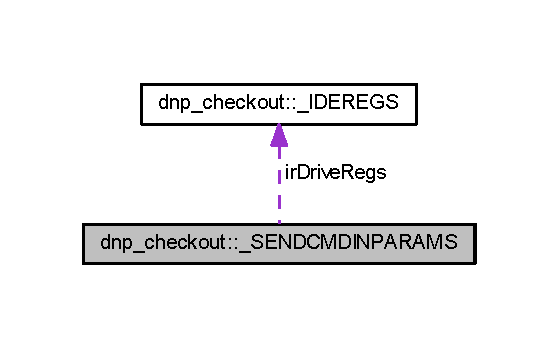
\includegraphics[width=268pt]{structdnp__checkout_1_1___s_e_n_d_c_m_d_i_n_p_a_r_a_m_s__coll__graph}
\end{center}
\end{figure}
\subsection*{Открытые атрибуты}
\begin{DoxyCompactItemize}
\item 
D\-W\-O\-R\-D \hyperlink{structdnp__checkout_1_1___s_e_n_d_c_m_d_i_n_p_a_r_a_m_s_a6746427c1348cf6c8caf775d740b0b6e}{c\-Buffer\-Size}
\item 
\hyperlink{namespacednp__checkout_ad6ca05b19c9b8b1d79306987d943d841}{I\-D\-E\-R\-E\-G\-S} \hyperlink{structdnp__checkout_1_1___s_e_n_d_c_m_d_i_n_p_a_r_a_m_s_ae8fed6d1ba296a07a93f0d0804f5a7ce}{ir\-Drive\-Regs}
\item 
B\-Y\-T\-E \hyperlink{structdnp__checkout_1_1___s_e_n_d_c_m_d_i_n_p_a_r_a_m_s_a92c04dce74c5ddb89d17844726031349}{b\-Drive\-Number}
\item 
B\-Y\-T\-E \hyperlink{structdnp__checkout_1_1___s_e_n_d_c_m_d_i_n_p_a_r_a_m_s_a579a92fced06869a0fb62a8679ce8b2d}{b\-Reserved} \mbox{[}3\mbox{]}
\item 
D\-W\-O\-R\-D \hyperlink{structdnp__checkout_1_1___s_e_n_d_c_m_d_i_n_p_a_r_a_m_s_a780a17af012cf9a376bcfa4411c3d037}{dw\-Reserved} \mbox{[}4\mbox{]}
\item 
B\-Y\-T\-E \hyperlink{structdnp__checkout_1_1___s_e_n_d_c_m_d_i_n_p_a_r_a_m_s_a1d496c0bac30e1c4ba551ec6ba6eaeac}{b\-Buffer} \mbox{[}1\mbox{]}
\end{DoxyCompactItemize}


\subsection{Данные класса}
\hypertarget{structdnp__checkout_1_1___s_e_n_d_c_m_d_i_n_p_a_r_a_m_s_a1d496c0bac30e1c4ba551ec6ba6eaeac}{\index{dnp\-\_\-checkout\-::\-\_\-\-S\-E\-N\-D\-C\-M\-D\-I\-N\-P\-A\-R\-A\-M\-S@{dnp\-\_\-checkout\-::\-\_\-\-S\-E\-N\-D\-C\-M\-D\-I\-N\-P\-A\-R\-A\-M\-S}!b\-Buffer@{b\-Buffer}}
\index{b\-Buffer@{b\-Buffer}!dnp_checkout::_SENDCMDINPARAMS@{dnp\-\_\-checkout\-::\-\_\-\-S\-E\-N\-D\-C\-M\-D\-I\-N\-P\-A\-R\-A\-M\-S}}
\subsubsection[{b\-Buffer}]{\setlength{\rightskip}{0pt plus 5cm}B\-Y\-T\-E dnp\-\_\-checkout\-::\-\_\-\-S\-E\-N\-D\-C\-M\-D\-I\-N\-P\-A\-R\-A\-M\-S\-::b\-Buffer\mbox{[}1\mbox{]}}}\label{structdnp__checkout_1_1___s_e_n_d_c_m_d_i_n_p_a_r_a_m_s_a1d496c0bac30e1c4ba551ec6ba6eaeac}
\hypertarget{structdnp__checkout_1_1___s_e_n_d_c_m_d_i_n_p_a_r_a_m_s_a92c04dce74c5ddb89d17844726031349}{\index{dnp\-\_\-checkout\-::\-\_\-\-S\-E\-N\-D\-C\-M\-D\-I\-N\-P\-A\-R\-A\-M\-S@{dnp\-\_\-checkout\-::\-\_\-\-S\-E\-N\-D\-C\-M\-D\-I\-N\-P\-A\-R\-A\-M\-S}!b\-Drive\-Number@{b\-Drive\-Number}}
\index{b\-Drive\-Number@{b\-Drive\-Number}!dnp_checkout::_SENDCMDINPARAMS@{dnp\-\_\-checkout\-::\-\_\-\-S\-E\-N\-D\-C\-M\-D\-I\-N\-P\-A\-R\-A\-M\-S}}
\subsubsection[{b\-Drive\-Number}]{\setlength{\rightskip}{0pt plus 5cm}B\-Y\-T\-E dnp\-\_\-checkout\-::\-\_\-\-S\-E\-N\-D\-C\-M\-D\-I\-N\-P\-A\-R\-A\-M\-S\-::b\-Drive\-Number}}\label{structdnp__checkout_1_1___s_e_n_d_c_m_d_i_n_p_a_r_a_m_s_a92c04dce74c5ddb89d17844726031349}
\hypertarget{structdnp__checkout_1_1___s_e_n_d_c_m_d_i_n_p_a_r_a_m_s_a579a92fced06869a0fb62a8679ce8b2d}{\index{dnp\-\_\-checkout\-::\-\_\-\-S\-E\-N\-D\-C\-M\-D\-I\-N\-P\-A\-R\-A\-M\-S@{dnp\-\_\-checkout\-::\-\_\-\-S\-E\-N\-D\-C\-M\-D\-I\-N\-P\-A\-R\-A\-M\-S}!b\-Reserved@{b\-Reserved}}
\index{b\-Reserved@{b\-Reserved}!dnp_checkout::_SENDCMDINPARAMS@{dnp\-\_\-checkout\-::\-\_\-\-S\-E\-N\-D\-C\-M\-D\-I\-N\-P\-A\-R\-A\-M\-S}}
\subsubsection[{b\-Reserved}]{\setlength{\rightskip}{0pt plus 5cm}B\-Y\-T\-E dnp\-\_\-checkout\-::\-\_\-\-S\-E\-N\-D\-C\-M\-D\-I\-N\-P\-A\-R\-A\-M\-S\-::b\-Reserved\mbox{[}3\mbox{]}}}\label{structdnp__checkout_1_1___s_e_n_d_c_m_d_i_n_p_a_r_a_m_s_a579a92fced06869a0fb62a8679ce8b2d}
\hypertarget{structdnp__checkout_1_1___s_e_n_d_c_m_d_i_n_p_a_r_a_m_s_a6746427c1348cf6c8caf775d740b0b6e}{\index{dnp\-\_\-checkout\-::\-\_\-\-S\-E\-N\-D\-C\-M\-D\-I\-N\-P\-A\-R\-A\-M\-S@{dnp\-\_\-checkout\-::\-\_\-\-S\-E\-N\-D\-C\-M\-D\-I\-N\-P\-A\-R\-A\-M\-S}!c\-Buffer\-Size@{c\-Buffer\-Size}}
\index{c\-Buffer\-Size@{c\-Buffer\-Size}!dnp_checkout::_SENDCMDINPARAMS@{dnp\-\_\-checkout\-::\-\_\-\-S\-E\-N\-D\-C\-M\-D\-I\-N\-P\-A\-R\-A\-M\-S}}
\subsubsection[{c\-Buffer\-Size}]{\setlength{\rightskip}{0pt plus 5cm}D\-W\-O\-R\-D dnp\-\_\-checkout\-::\-\_\-\-S\-E\-N\-D\-C\-M\-D\-I\-N\-P\-A\-R\-A\-M\-S\-::c\-Buffer\-Size}}\label{structdnp__checkout_1_1___s_e_n_d_c_m_d_i_n_p_a_r_a_m_s_a6746427c1348cf6c8caf775d740b0b6e}
\hypertarget{structdnp__checkout_1_1___s_e_n_d_c_m_d_i_n_p_a_r_a_m_s_a780a17af012cf9a376bcfa4411c3d037}{\index{dnp\-\_\-checkout\-::\-\_\-\-S\-E\-N\-D\-C\-M\-D\-I\-N\-P\-A\-R\-A\-M\-S@{dnp\-\_\-checkout\-::\-\_\-\-S\-E\-N\-D\-C\-M\-D\-I\-N\-P\-A\-R\-A\-M\-S}!dw\-Reserved@{dw\-Reserved}}
\index{dw\-Reserved@{dw\-Reserved}!dnp_checkout::_SENDCMDINPARAMS@{dnp\-\_\-checkout\-::\-\_\-\-S\-E\-N\-D\-C\-M\-D\-I\-N\-P\-A\-R\-A\-M\-S}}
\subsubsection[{dw\-Reserved}]{\setlength{\rightskip}{0pt plus 5cm}D\-W\-O\-R\-D dnp\-\_\-checkout\-::\-\_\-\-S\-E\-N\-D\-C\-M\-D\-I\-N\-P\-A\-R\-A\-M\-S\-::dw\-Reserved\mbox{[}4\mbox{]}}}\label{structdnp__checkout_1_1___s_e_n_d_c_m_d_i_n_p_a_r_a_m_s_a780a17af012cf9a376bcfa4411c3d037}
\hypertarget{structdnp__checkout_1_1___s_e_n_d_c_m_d_i_n_p_a_r_a_m_s_ae8fed6d1ba296a07a93f0d0804f5a7ce}{\index{dnp\-\_\-checkout\-::\-\_\-\-S\-E\-N\-D\-C\-M\-D\-I\-N\-P\-A\-R\-A\-M\-S@{dnp\-\_\-checkout\-::\-\_\-\-S\-E\-N\-D\-C\-M\-D\-I\-N\-P\-A\-R\-A\-M\-S}!ir\-Drive\-Regs@{ir\-Drive\-Regs}}
\index{ir\-Drive\-Regs@{ir\-Drive\-Regs}!dnp_checkout::_SENDCMDINPARAMS@{dnp\-\_\-checkout\-::\-\_\-\-S\-E\-N\-D\-C\-M\-D\-I\-N\-P\-A\-R\-A\-M\-S}}
\subsubsection[{ir\-Drive\-Regs}]{\setlength{\rightskip}{0pt plus 5cm}{\bf I\-D\-E\-R\-E\-G\-S} dnp\-\_\-checkout\-::\-\_\-\-S\-E\-N\-D\-C\-M\-D\-I\-N\-P\-A\-R\-A\-M\-S\-::ir\-Drive\-Regs}}\label{structdnp__checkout_1_1___s_e_n_d_c_m_d_i_n_p_a_r_a_m_s_ae8fed6d1ba296a07a93f0d0804f5a7ce}


Объявления и описания членов структуры находятся в файле\-:\begin{DoxyCompactItemize}
\item 
src/\hyperlink{dnp__checkout_8cpp}{dnp\-\_\-checkout.\-cpp}\end{DoxyCompactItemize}

\hypertarget{structdnp__checkout_1_1___s_e_n_d_c_m_d_o_u_t_p_a_r_a_m_s}{\section{Структура dnp\-\_\-checkout\-:\-:\-\_\-\-S\-E\-N\-D\-C\-M\-D\-O\-U\-T\-P\-A\-R\-A\-M\-S}
\label{structdnp__checkout_1_1___s_e_n_d_c_m_d_o_u_t_p_a_r_a_m_s}\index{dnp\-\_\-checkout\-::\-\_\-\-S\-E\-N\-D\-C\-M\-D\-O\-U\-T\-P\-A\-R\-A\-M\-S@{dnp\-\_\-checkout\-::\-\_\-\-S\-E\-N\-D\-C\-M\-D\-O\-U\-T\-P\-A\-R\-A\-M\-S}}
}


Граф связей класса dnp\-\_\-checkout\-:\-:\-\_\-\-S\-E\-N\-D\-C\-M\-D\-O\-U\-T\-P\-A\-R\-A\-M\-S\-:
\nopagebreak
\begin{figure}[H]
\begin{center}
\leavevmode
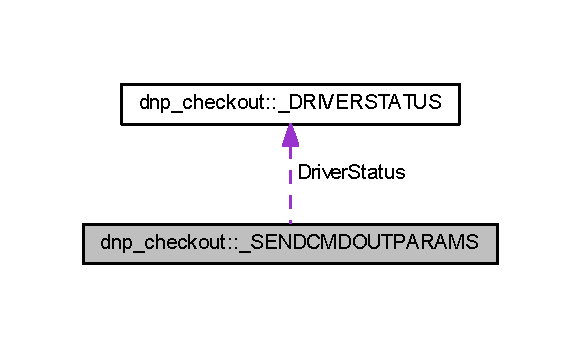
\includegraphics[width=279pt]{structdnp__checkout_1_1___s_e_n_d_c_m_d_o_u_t_p_a_r_a_m_s__coll__graph}
\end{center}
\end{figure}
\subsection*{Открытые атрибуты}
\begin{DoxyCompactItemize}
\item 
D\-W\-O\-R\-D \hyperlink{structdnp__checkout_1_1___s_e_n_d_c_m_d_o_u_t_p_a_r_a_m_s_afa3ffd902c48f6d0a5eb15214702bda0}{c\-Buffer\-Size}
\item 
\hyperlink{namespacednp__checkout_a4a8d9b7c57ae5e7d0d88f7a5be282c57}{D\-R\-I\-V\-E\-R\-S\-T\-A\-T\-U\-S} \hyperlink{structdnp__checkout_1_1___s_e_n_d_c_m_d_o_u_t_p_a_r_a_m_s_a2d8a7d4790efc42354257b48a3dccc01}{Driver\-Status}
\item 
B\-Y\-T\-E \hyperlink{structdnp__checkout_1_1___s_e_n_d_c_m_d_o_u_t_p_a_r_a_m_s_aef7cba9886b5a6307a39a884bc0fab3d}{b\-Buffer} \mbox{[}1\mbox{]}
\end{DoxyCompactItemize}


\subsection{Данные класса}
\hypertarget{structdnp__checkout_1_1___s_e_n_d_c_m_d_o_u_t_p_a_r_a_m_s_aef7cba9886b5a6307a39a884bc0fab3d}{\index{dnp\-\_\-checkout\-::\-\_\-\-S\-E\-N\-D\-C\-M\-D\-O\-U\-T\-P\-A\-R\-A\-M\-S@{dnp\-\_\-checkout\-::\-\_\-\-S\-E\-N\-D\-C\-M\-D\-O\-U\-T\-P\-A\-R\-A\-M\-S}!b\-Buffer@{b\-Buffer}}
\index{b\-Buffer@{b\-Buffer}!dnp_checkout::_SENDCMDOUTPARAMS@{dnp\-\_\-checkout\-::\-\_\-\-S\-E\-N\-D\-C\-M\-D\-O\-U\-T\-P\-A\-R\-A\-M\-S}}
\subsubsection[{b\-Buffer}]{\setlength{\rightskip}{0pt plus 5cm}B\-Y\-T\-E dnp\-\_\-checkout\-::\-\_\-\-S\-E\-N\-D\-C\-M\-D\-O\-U\-T\-P\-A\-R\-A\-M\-S\-::b\-Buffer\mbox{[}1\mbox{]}}}\label{structdnp__checkout_1_1___s_e_n_d_c_m_d_o_u_t_p_a_r_a_m_s_aef7cba9886b5a6307a39a884bc0fab3d}
\hypertarget{structdnp__checkout_1_1___s_e_n_d_c_m_d_o_u_t_p_a_r_a_m_s_afa3ffd902c48f6d0a5eb15214702bda0}{\index{dnp\-\_\-checkout\-::\-\_\-\-S\-E\-N\-D\-C\-M\-D\-O\-U\-T\-P\-A\-R\-A\-M\-S@{dnp\-\_\-checkout\-::\-\_\-\-S\-E\-N\-D\-C\-M\-D\-O\-U\-T\-P\-A\-R\-A\-M\-S}!c\-Buffer\-Size@{c\-Buffer\-Size}}
\index{c\-Buffer\-Size@{c\-Buffer\-Size}!dnp_checkout::_SENDCMDOUTPARAMS@{dnp\-\_\-checkout\-::\-\_\-\-S\-E\-N\-D\-C\-M\-D\-O\-U\-T\-P\-A\-R\-A\-M\-S}}
\subsubsection[{c\-Buffer\-Size}]{\setlength{\rightskip}{0pt plus 5cm}D\-W\-O\-R\-D dnp\-\_\-checkout\-::\-\_\-\-S\-E\-N\-D\-C\-M\-D\-O\-U\-T\-P\-A\-R\-A\-M\-S\-::c\-Buffer\-Size}}\label{structdnp__checkout_1_1___s_e_n_d_c_m_d_o_u_t_p_a_r_a_m_s_afa3ffd902c48f6d0a5eb15214702bda0}
\hypertarget{structdnp__checkout_1_1___s_e_n_d_c_m_d_o_u_t_p_a_r_a_m_s_a2d8a7d4790efc42354257b48a3dccc01}{\index{dnp\-\_\-checkout\-::\-\_\-\-S\-E\-N\-D\-C\-M\-D\-O\-U\-T\-P\-A\-R\-A\-M\-S@{dnp\-\_\-checkout\-::\-\_\-\-S\-E\-N\-D\-C\-M\-D\-O\-U\-T\-P\-A\-R\-A\-M\-S}!Driver\-Status@{Driver\-Status}}
\index{Driver\-Status@{Driver\-Status}!dnp_checkout::_SENDCMDOUTPARAMS@{dnp\-\_\-checkout\-::\-\_\-\-S\-E\-N\-D\-C\-M\-D\-O\-U\-T\-P\-A\-R\-A\-M\-S}}
\subsubsection[{Driver\-Status}]{\setlength{\rightskip}{0pt plus 5cm}{\bf D\-R\-I\-V\-E\-R\-S\-T\-A\-T\-U\-S} dnp\-\_\-checkout\-::\-\_\-\-S\-E\-N\-D\-C\-M\-D\-O\-U\-T\-P\-A\-R\-A\-M\-S\-::\-Driver\-Status}}\label{structdnp__checkout_1_1___s_e_n_d_c_m_d_o_u_t_p_a_r_a_m_s_a2d8a7d4790efc42354257b48a3dccc01}


Объявления и описания членов структуры находятся в файле\-:\begin{DoxyCompactItemize}
\item 
src/\hyperlink{dnp__checkout_8cpp}{dnp\-\_\-checkout.\-cpp}\end{DoxyCompactItemize}

\hypertarget{structdnp__checkout_1_1___s_r_b___i_o___c_o_n_t_r_o_l}{\section{Структура dnp\-\_\-checkout\-:\-:\-\_\-\-S\-R\-B\-\_\-\-I\-O\-\_\-\-C\-O\-N\-T\-R\-O\-L}
\label{structdnp__checkout_1_1___s_r_b___i_o___c_o_n_t_r_o_l}\index{dnp\-\_\-checkout\-::\-\_\-\-S\-R\-B\-\_\-\-I\-O\-\_\-\-C\-O\-N\-T\-R\-O\-L@{dnp\-\_\-checkout\-::\-\_\-\-S\-R\-B\-\_\-\-I\-O\-\_\-\-C\-O\-N\-T\-R\-O\-L}}
}
\subsection*{Открытые атрибуты}
\begin{DoxyCompactItemize}
\item 
U\-L\-O\-N\-G \hyperlink{structdnp__checkout_1_1___s_r_b___i_o___c_o_n_t_r_o_l_a425891ae016e7761e283cb87a4e1dd04}{Header\-Length}
\item 
U\-C\-H\-A\-R \hyperlink{structdnp__checkout_1_1___s_r_b___i_o___c_o_n_t_r_o_l_ab20268b355c4216b3496d8a603ece077}{Signature} \mbox{[}8\mbox{]}
\item 
U\-L\-O\-N\-G \hyperlink{structdnp__checkout_1_1___s_r_b___i_o___c_o_n_t_r_o_l_a9f2367e5508f7001e0da9439580dbfd5}{Timeout}
\item 
U\-L\-O\-N\-G \hyperlink{structdnp__checkout_1_1___s_r_b___i_o___c_o_n_t_r_o_l_a4eba66ca654685ad1cd43ae247157d0e}{Control\-Code}
\item 
U\-L\-O\-N\-G \hyperlink{structdnp__checkout_1_1___s_r_b___i_o___c_o_n_t_r_o_l_a516339f7092eda246bf9a48342330f50}{Return\-Code}
\item 
U\-L\-O\-N\-G \hyperlink{structdnp__checkout_1_1___s_r_b___i_o___c_o_n_t_r_o_l_a19604bd52e959c15f32088462f3277d7}{Length}
\end{DoxyCompactItemize}


\subsection{Данные класса}
\hypertarget{structdnp__checkout_1_1___s_r_b___i_o___c_o_n_t_r_o_l_a4eba66ca654685ad1cd43ae247157d0e}{\index{dnp\-\_\-checkout\-::\-\_\-\-S\-R\-B\-\_\-\-I\-O\-\_\-\-C\-O\-N\-T\-R\-O\-L@{dnp\-\_\-checkout\-::\-\_\-\-S\-R\-B\-\_\-\-I\-O\-\_\-\-C\-O\-N\-T\-R\-O\-L}!Control\-Code@{Control\-Code}}
\index{Control\-Code@{Control\-Code}!dnp_checkout::_SRB_IO_CONTROL@{dnp\-\_\-checkout\-::\-\_\-\-S\-R\-B\-\_\-\-I\-O\-\_\-\-C\-O\-N\-T\-R\-O\-L}}
\subsubsection[{Control\-Code}]{\setlength{\rightskip}{0pt plus 5cm}U\-L\-O\-N\-G dnp\-\_\-checkout\-::\-\_\-\-S\-R\-B\-\_\-\-I\-O\-\_\-\-C\-O\-N\-T\-R\-O\-L\-::\-Control\-Code}}\label{structdnp__checkout_1_1___s_r_b___i_o___c_o_n_t_r_o_l_a4eba66ca654685ad1cd43ae247157d0e}
\hypertarget{structdnp__checkout_1_1___s_r_b___i_o___c_o_n_t_r_o_l_a425891ae016e7761e283cb87a4e1dd04}{\index{dnp\-\_\-checkout\-::\-\_\-\-S\-R\-B\-\_\-\-I\-O\-\_\-\-C\-O\-N\-T\-R\-O\-L@{dnp\-\_\-checkout\-::\-\_\-\-S\-R\-B\-\_\-\-I\-O\-\_\-\-C\-O\-N\-T\-R\-O\-L}!Header\-Length@{Header\-Length}}
\index{Header\-Length@{Header\-Length}!dnp_checkout::_SRB_IO_CONTROL@{dnp\-\_\-checkout\-::\-\_\-\-S\-R\-B\-\_\-\-I\-O\-\_\-\-C\-O\-N\-T\-R\-O\-L}}
\subsubsection[{Header\-Length}]{\setlength{\rightskip}{0pt plus 5cm}U\-L\-O\-N\-G dnp\-\_\-checkout\-::\-\_\-\-S\-R\-B\-\_\-\-I\-O\-\_\-\-C\-O\-N\-T\-R\-O\-L\-::\-Header\-Length}}\label{structdnp__checkout_1_1___s_r_b___i_o___c_o_n_t_r_o_l_a425891ae016e7761e283cb87a4e1dd04}
\hypertarget{structdnp__checkout_1_1___s_r_b___i_o___c_o_n_t_r_o_l_a19604bd52e959c15f32088462f3277d7}{\index{dnp\-\_\-checkout\-::\-\_\-\-S\-R\-B\-\_\-\-I\-O\-\_\-\-C\-O\-N\-T\-R\-O\-L@{dnp\-\_\-checkout\-::\-\_\-\-S\-R\-B\-\_\-\-I\-O\-\_\-\-C\-O\-N\-T\-R\-O\-L}!Length@{Length}}
\index{Length@{Length}!dnp_checkout::_SRB_IO_CONTROL@{dnp\-\_\-checkout\-::\-\_\-\-S\-R\-B\-\_\-\-I\-O\-\_\-\-C\-O\-N\-T\-R\-O\-L}}
\subsubsection[{Length}]{\setlength{\rightskip}{0pt plus 5cm}U\-L\-O\-N\-G dnp\-\_\-checkout\-::\-\_\-\-S\-R\-B\-\_\-\-I\-O\-\_\-\-C\-O\-N\-T\-R\-O\-L\-::\-Length}}\label{structdnp__checkout_1_1___s_r_b___i_o___c_o_n_t_r_o_l_a19604bd52e959c15f32088462f3277d7}
\hypertarget{structdnp__checkout_1_1___s_r_b___i_o___c_o_n_t_r_o_l_a516339f7092eda246bf9a48342330f50}{\index{dnp\-\_\-checkout\-::\-\_\-\-S\-R\-B\-\_\-\-I\-O\-\_\-\-C\-O\-N\-T\-R\-O\-L@{dnp\-\_\-checkout\-::\-\_\-\-S\-R\-B\-\_\-\-I\-O\-\_\-\-C\-O\-N\-T\-R\-O\-L}!Return\-Code@{Return\-Code}}
\index{Return\-Code@{Return\-Code}!dnp_checkout::_SRB_IO_CONTROL@{dnp\-\_\-checkout\-::\-\_\-\-S\-R\-B\-\_\-\-I\-O\-\_\-\-C\-O\-N\-T\-R\-O\-L}}
\subsubsection[{Return\-Code}]{\setlength{\rightskip}{0pt plus 5cm}U\-L\-O\-N\-G dnp\-\_\-checkout\-::\-\_\-\-S\-R\-B\-\_\-\-I\-O\-\_\-\-C\-O\-N\-T\-R\-O\-L\-::\-Return\-Code}}\label{structdnp__checkout_1_1___s_r_b___i_o___c_o_n_t_r_o_l_a516339f7092eda246bf9a48342330f50}
\hypertarget{structdnp__checkout_1_1___s_r_b___i_o___c_o_n_t_r_o_l_ab20268b355c4216b3496d8a603ece077}{\index{dnp\-\_\-checkout\-::\-\_\-\-S\-R\-B\-\_\-\-I\-O\-\_\-\-C\-O\-N\-T\-R\-O\-L@{dnp\-\_\-checkout\-::\-\_\-\-S\-R\-B\-\_\-\-I\-O\-\_\-\-C\-O\-N\-T\-R\-O\-L}!Signature@{Signature}}
\index{Signature@{Signature}!dnp_checkout::_SRB_IO_CONTROL@{dnp\-\_\-checkout\-::\-\_\-\-S\-R\-B\-\_\-\-I\-O\-\_\-\-C\-O\-N\-T\-R\-O\-L}}
\subsubsection[{Signature}]{\setlength{\rightskip}{0pt plus 5cm}U\-C\-H\-A\-R dnp\-\_\-checkout\-::\-\_\-\-S\-R\-B\-\_\-\-I\-O\-\_\-\-C\-O\-N\-T\-R\-O\-L\-::\-Signature\mbox{[}8\mbox{]}}}\label{structdnp__checkout_1_1___s_r_b___i_o___c_o_n_t_r_o_l_ab20268b355c4216b3496d8a603ece077}
\hypertarget{structdnp__checkout_1_1___s_r_b___i_o___c_o_n_t_r_o_l_a9f2367e5508f7001e0da9439580dbfd5}{\index{dnp\-\_\-checkout\-::\-\_\-\-S\-R\-B\-\_\-\-I\-O\-\_\-\-C\-O\-N\-T\-R\-O\-L@{dnp\-\_\-checkout\-::\-\_\-\-S\-R\-B\-\_\-\-I\-O\-\_\-\-C\-O\-N\-T\-R\-O\-L}!Timeout@{Timeout}}
\index{Timeout@{Timeout}!dnp_checkout::_SRB_IO_CONTROL@{dnp\-\_\-checkout\-::\-\_\-\-S\-R\-B\-\_\-\-I\-O\-\_\-\-C\-O\-N\-T\-R\-O\-L}}
\subsubsection[{Timeout}]{\setlength{\rightskip}{0pt plus 5cm}U\-L\-O\-N\-G dnp\-\_\-checkout\-::\-\_\-\-S\-R\-B\-\_\-\-I\-O\-\_\-\-C\-O\-N\-T\-R\-O\-L\-::\-Timeout}}\label{structdnp__checkout_1_1___s_r_b___i_o___c_o_n_t_r_o_l_a9f2367e5508f7001e0da9439580dbfd5}


Объявления и описания членов структуры находятся в файле\-:\begin{DoxyCompactItemize}
\item 
src/\hyperlink{dnp__checkout_8cpp}{dnp\-\_\-checkout.\-cpp}\end{DoxyCompactItemize}

\hypertarget{classxyplot_1_1_a_l_l___p_l_o_t_s__}{\section{Класс xyplot\-:\-:A\-L\-L\-\_\-\-P\-L\-O\-T\-S\-\_\-}
\label{classxyplot_1_1_a_l_l___p_l_o_t_s__}\index{xyplot\-::\-A\-L\-L\-\_\-\-P\-L\-O\-T\-S\-\_\-@{xyplot\-::\-A\-L\-L\-\_\-\-P\-L\-O\-T\-S\-\_\-}}
}


Класс дескриптор для всех экземпляров 2\-D графики  




{\ttfamily \#include $<$X\-Y\-Plot\-Wrapper.\-h$>$}



Граф наследования\-:xyplot\-:\-:A\-L\-L\-\_\-\-P\-L\-O\-T\-S\-\_\-\-:\nopagebreak
\begin{figure}[H]
\begin{center}
\leavevmode
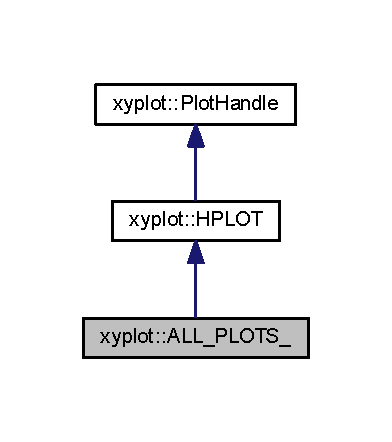
\includegraphics[width=188pt]{classxyplot_1_1_a_l_l___p_l_o_t_s____inherit__graph}
\end{center}
\end{figure}


Граф связей класса xyplot\-:\-:A\-L\-L\-\_\-\-P\-L\-O\-T\-S\-\_\-\-:\nopagebreak
\begin{figure}[H]
\begin{center}
\leavevmode
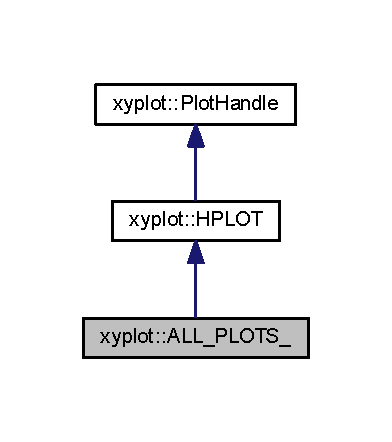
\includegraphics[width=188pt]{classxyplot_1_1_a_l_l___p_l_o_t_s____coll__graph}
\end{center}
\end{figure}
\subsection*{Открытые члены}
\begin{DoxyCompactItemize}
\item 
\hyperlink{classxyplot_1_1_a_l_l___p_l_o_t_s___a6dc10365227f717e36d3bb55ac1e31d2}{A\-L\-L\-\_\-\-P\-L\-O\-T\-S\-\_\-} ()
\end{DoxyCompactItemize}
\subsection*{Дополнительные унаследованные члены}


\subsection{Подробное описание}
Класс дескриптор для всех экземпляров 2\-D графики 

\subsection{Конструктор(ы)}
\hypertarget{classxyplot_1_1_a_l_l___p_l_o_t_s___a6dc10365227f717e36d3bb55ac1e31d2}{\index{xyplot\-::\-A\-L\-L\-\_\-\-P\-L\-O\-T\-S\-\_\-@{xyplot\-::\-A\-L\-L\-\_\-\-P\-L\-O\-T\-S\-\_\-}!A\-L\-L\-\_\-\-P\-L\-O\-T\-S\-\_\-@{A\-L\-L\-\_\-\-P\-L\-O\-T\-S\-\_\-}}
\index{A\-L\-L\-\_\-\-P\-L\-O\-T\-S\-\_\-@{A\-L\-L\-\_\-\-P\-L\-O\-T\-S\-\_\-}!xyplot::ALL_PLOTS_@{xyplot\-::\-A\-L\-L\-\_\-\-P\-L\-O\-T\-S\-\_\-}}
\subsubsection[{A\-L\-L\-\_\-\-P\-L\-O\-T\-S\-\_\-}]{\setlength{\rightskip}{0pt plus 5cm}xyplot\-::\-A\-L\-L\-\_\-\-P\-L\-O\-T\-S\-\_\-\-::\-A\-L\-L\-\_\-\-P\-L\-O\-T\-S\-\_\- (
\begin{DoxyParamCaption}
{}
\end{DoxyParamCaption}
)\hspace{0.3cm}{\ttfamily [inline]}}}\label{classxyplot_1_1_a_l_l___p_l_o_t_s___a6dc10365227f717e36d3bb55ac1e31d2}
Конструктор по умолчанию. 

Объявления и описания членов класса находятся в файле\-:\begin{DoxyCompactItemize}
\item 
src/\hyperlink{_x_y_plot_wrapper_8h}{X\-Y\-Plot\-Wrapper.\-h}\end{DoxyCompactItemize}

\hypertarget{classxyplot_1_1_a_l_l___p_r_o_f_i_l_e_s}{\section{Класс xyplot\-:\-:A\-L\-L\-\_\-\-P\-R\-O\-F\-I\-L\-E\-S}
\label{classxyplot_1_1_a_l_l___p_r_o_f_i_l_e_s}\index{xyplot\-::\-A\-L\-L\-\_\-\-P\-R\-O\-F\-I\-L\-E\-S@{xyplot\-::\-A\-L\-L\-\_\-\-P\-R\-O\-F\-I\-L\-E\-S}}
}


Класс дескриптор для всех профилей 2\-D графики  




{\ttfamily \#include $<$X\-Y\-Plot\-Wrapper.\-h$>$}



Граф наследования\-:xyplot\-:\-:A\-L\-L\-\_\-\-P\-R\-O\-F\-I\-L\-E\-S\-:\nopagebreak
\begin{figure}[H]
\begin{center}
\leavevmode
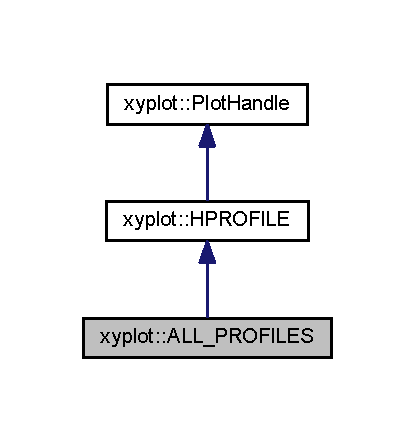
\includegraphics[width=199pt]{classxyplot_1_1_a_l_l___p_r_o_f_i_l_e_s__inherit__graph}
\end{center}
\end{figure}


Граф связей класса xyplot\-:\-:A\-L\-L\-\_\-\-P\-R\-O\-F\-I\-L\-E\-S\-:\nopagebreak
\begin{figure}[H]
\begin{center}
\leavevmode
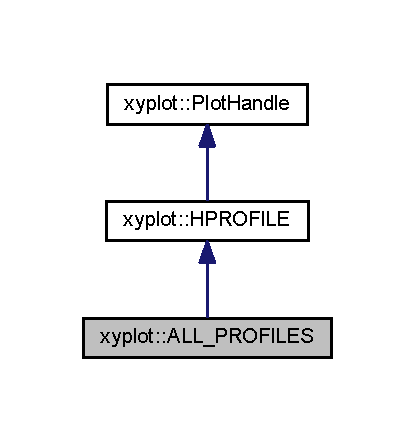
\includegraphics[width=199pt]{classxyplot_1_1_a_l_l___p_r_o_f_i_l_e_s__coll__graph}
\end{center}
\end{figure}
\subsection*{Открытые члены}
\begin{DoxyCompactItemize}
\item 
\hyperlink{classxyplot_1_1_a_l_l___p_r_o_f_i_l_e_s_a22b93a39697ac9145e378bf161be1639}{A\-L\-L\-\_\-\-P\-R\-O\-F\-I\-L\-E\-S} ()
\end{DoxyCompactItemize}
\subsection*{Дополнительные унаследованные члены}


\subsection{Подробное описание}
Класс дескриптор для всех профилей 2\-D графики 

\subsection{Конструктор(ы)}
\hypertarget{classxyplot_1_1_a_l_l___p_r_o_f_i_l_e_s_a22b93a39697ac9145e378bf161be1639}{\index{xyplot\-::\-A\-L\-L\-\_\-\-P\-R\-O\-F\-I\-L\-E\-S@{xyplot\-::\-A\-L\-L\-\_\-\-P\-R\-O\-F\-I\-L\-E\-S}!A\-L\-L\-\_\-\-P\-R\-O\-F\-I\-L\-E\-S@{A\-L\-L\-\_\-\-P\-R\-O\-F\-I\-L\-E\-S}}
\index{A\-L\-L\-\_\-\-P\-R\-O\-F\-I\-L\-E\-S@{A\-L\-L\-\_\-\-P\-R\-O\-F\-I\-L\-E\-S}!xyplot::ALL_PROFILES@{xyplot\-::\-A\-L\-L\-\_\-\-P\-R\-O\-F\-I\-L\-E\-S}}
\subsubsection[{A\-L\-L\-\_\-\-P\-R\-O\-F\-I\-L\-E\-S}]{\setlength{\rightskip}{0pt plus 5cm}xyplot\-::\-A\-L\-L\-\_\-\-P\-R\-O\-F\-I\-L\-E\-S\-::\-A\-L\-L\-\_\-\-P\-R\-O\-F\-I\-L\-E\-S (
\begin{DoxyParamCaption}
{}
\end{DoxyParamCaption}
)\hspace{0.3cm}{\ttfamily [inline]}}}\label{classxyplot_1_1_a_l_l___p_r_o_f_i_l_e_s_a22b93a39697ac9145e378bf161be1639}


Объявления и описания членов класса находятся в файле\-:\begin{DoxyCompactItemize}
\item 
src/\hyperlink{_x_y_plot_wrapper_8h}{X\-Y\-Plot\-Wrapper.\-h}\end{DoxyCompactItemize}

\hypertarget{classxyplot_1_1_a_l_l___r_e_g_i_o_n_s__}{\section{Класс xyplot\-:\-:A\-L\-L\-\_\-\-R\-E\-G\-I\-O\-N\-S\-\_\-}
\label{classxyplot_1_1_a_l_l___r_e_g_i_o_n_s__}\index{xyplot\-::\-A\-L\-L\-\_\-\-R\-E\-G\-I\-O\-N\-S\-\_\-@{xyplot\-::\-A\-L\-L\-\_\-\-R\-E\-G\-I\-O\-N\-S\-\_\-}}
}


Класс дескриптор всех регионов  




{\ttfamily \#include $<$X\-Y\-Plot\-Wrapper.\-h$>$}



Граф наследования\-:xyplot\-:\-:A\-L\-L\-\_\-\-R\-E\-G\-I\-O\-N\-S\-\_\-\-:\nopagebreak
\begin{figure}[H]
\begin{center}
\leavevmode
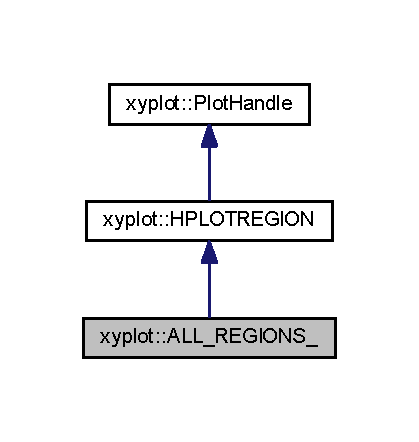
\includegraphics[width=201pt]{classxyplot_1_1_a_l_l___r_e_g_i_o_n_s____inherit__graph}
\end{center}
\end{figure}


Граф связей класса xyplot\-:\-:A\-L\-L\-\_\-\-R\-E\-G\-I\-O\-N\-S\-\_\-\-:\nopagebreak
\begin{figure}[H]
\begin{center}
\leavevmode
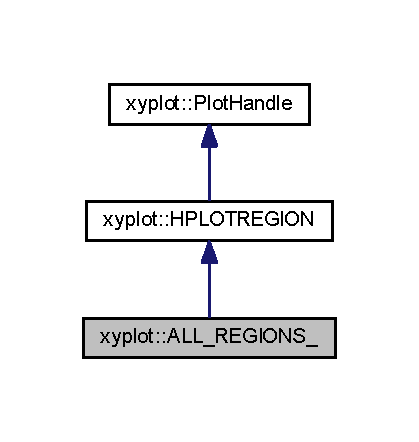
\includegraphics[width=201pt]{classxyplot_1_1_a_l_l___r_e_g_i_o_n_s____coll__graph}
\end{center}
\end{figure}
\subsection*{Открытые члены}
\begin{DoxyCompactItemize}
\item 
\hyperlink{classxyplot_1_1_a_l_l___r_e_g_i_o_n_s___a7e44573293e534d920cf1b8ae7edb22e}{A\-L\-L\-\_\-\-R\-E\-G\-I\-O\-N\-S\-\_\-} ()
\end{DoxyCompactItemize}
\subsection*{Дополнительные унаследованные члены}


\subsection{Подробное описание}
Класс дескриптор всех регионов 

\subsection{Конструктор(ы)}
\hypertarget{classxyplot_1_1_a_l_l___r_e_g_i_o_n_s___a7e44573293e534d920cf1b8ae7edb22e}{\index{xyplot\-::\-A\-L\-L\-\_\-\-R\-E\-G\-I\-O\-N\-S\-\_\-@{xyplot\-::\-A\-L\-L\-\_\-\-R\-E\-G\-I\-O\-N\-S\-\_\-}!A\-L\-L\-\_\-\-R\-E\-G\-I\-O\-N\-S\-\_\-@{A\-L\-L\-\_\-\-R\-E\-G\-I\-O\-N\-S\-\_\-}}
\index{A\-L\-L\-\_\-\-R\-E\-G\-I\-O\-N\-S\-\_\-@{A\-L\-L\-\_\-\-R\-E\-G\-I\-O\-N\-S\-\_\-}!xyplot::ALL_REGIONS_@{xyplot\-::\-A\-L\-L\-\_\-\-R\-E\-G\-I\-O\-N\-S\-\_\-}}
\subsubsection[{A\-L\-L\-\_\-\-R\-E\-G\-I\-O\-N\-S\-\_\-}]{\setlength{\rightskip}{0pt plus 5cm}xyplot\-::\-A\-L\-L\-\_\-\-R\-E\-G\-I\-O\-N\-S\-\_\-\-::\-A\-L\-L\-\_\-\-R\-E\-G\-I\-O\-N\-S\-\_\- (
\begin{DoxyParamCaption}
{}
\end{DoxyParamCaption}
)\hspace{0.3cm}{\ttfamily [inline]}}}\label{classxyplot_1_1_a_l_l___r_e_g_i_o_n_s___a7e44573293e534d920cf1b8ae7edb22e}


Объявления и описания членов класса находятся в файле\-:\begin{DoxyCompactItemize}
\item 
src/\hyperlink{_x_y_plot_wrapper_8h}{X\-Y\-Plot\-Wrapper.\-h}\end{DoxyCompactItemize}

\hypertarget{class_axis}{\section{Класс Axis}
\label{class_axis}\index{Axis@{Axis}}
}


{\ttfamily \#include $<$Axis.\-h$>$}



Граф наследования\-:Axis\-:
\nopagebreak
\begin{figure}[H]
\begin{center}
\leavevmode
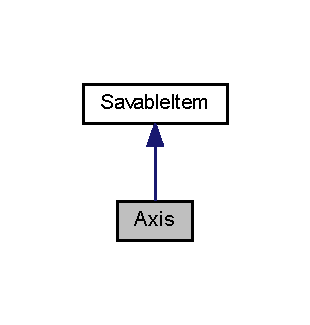
\includegraphics[width=149pt]{class_axis__inherit__graph}
\end{center}
\end{figure}


Граф связей класса Axis\-:
\nopagebreak
\begin{figure}[H]
\begin{center}
\leavevmode
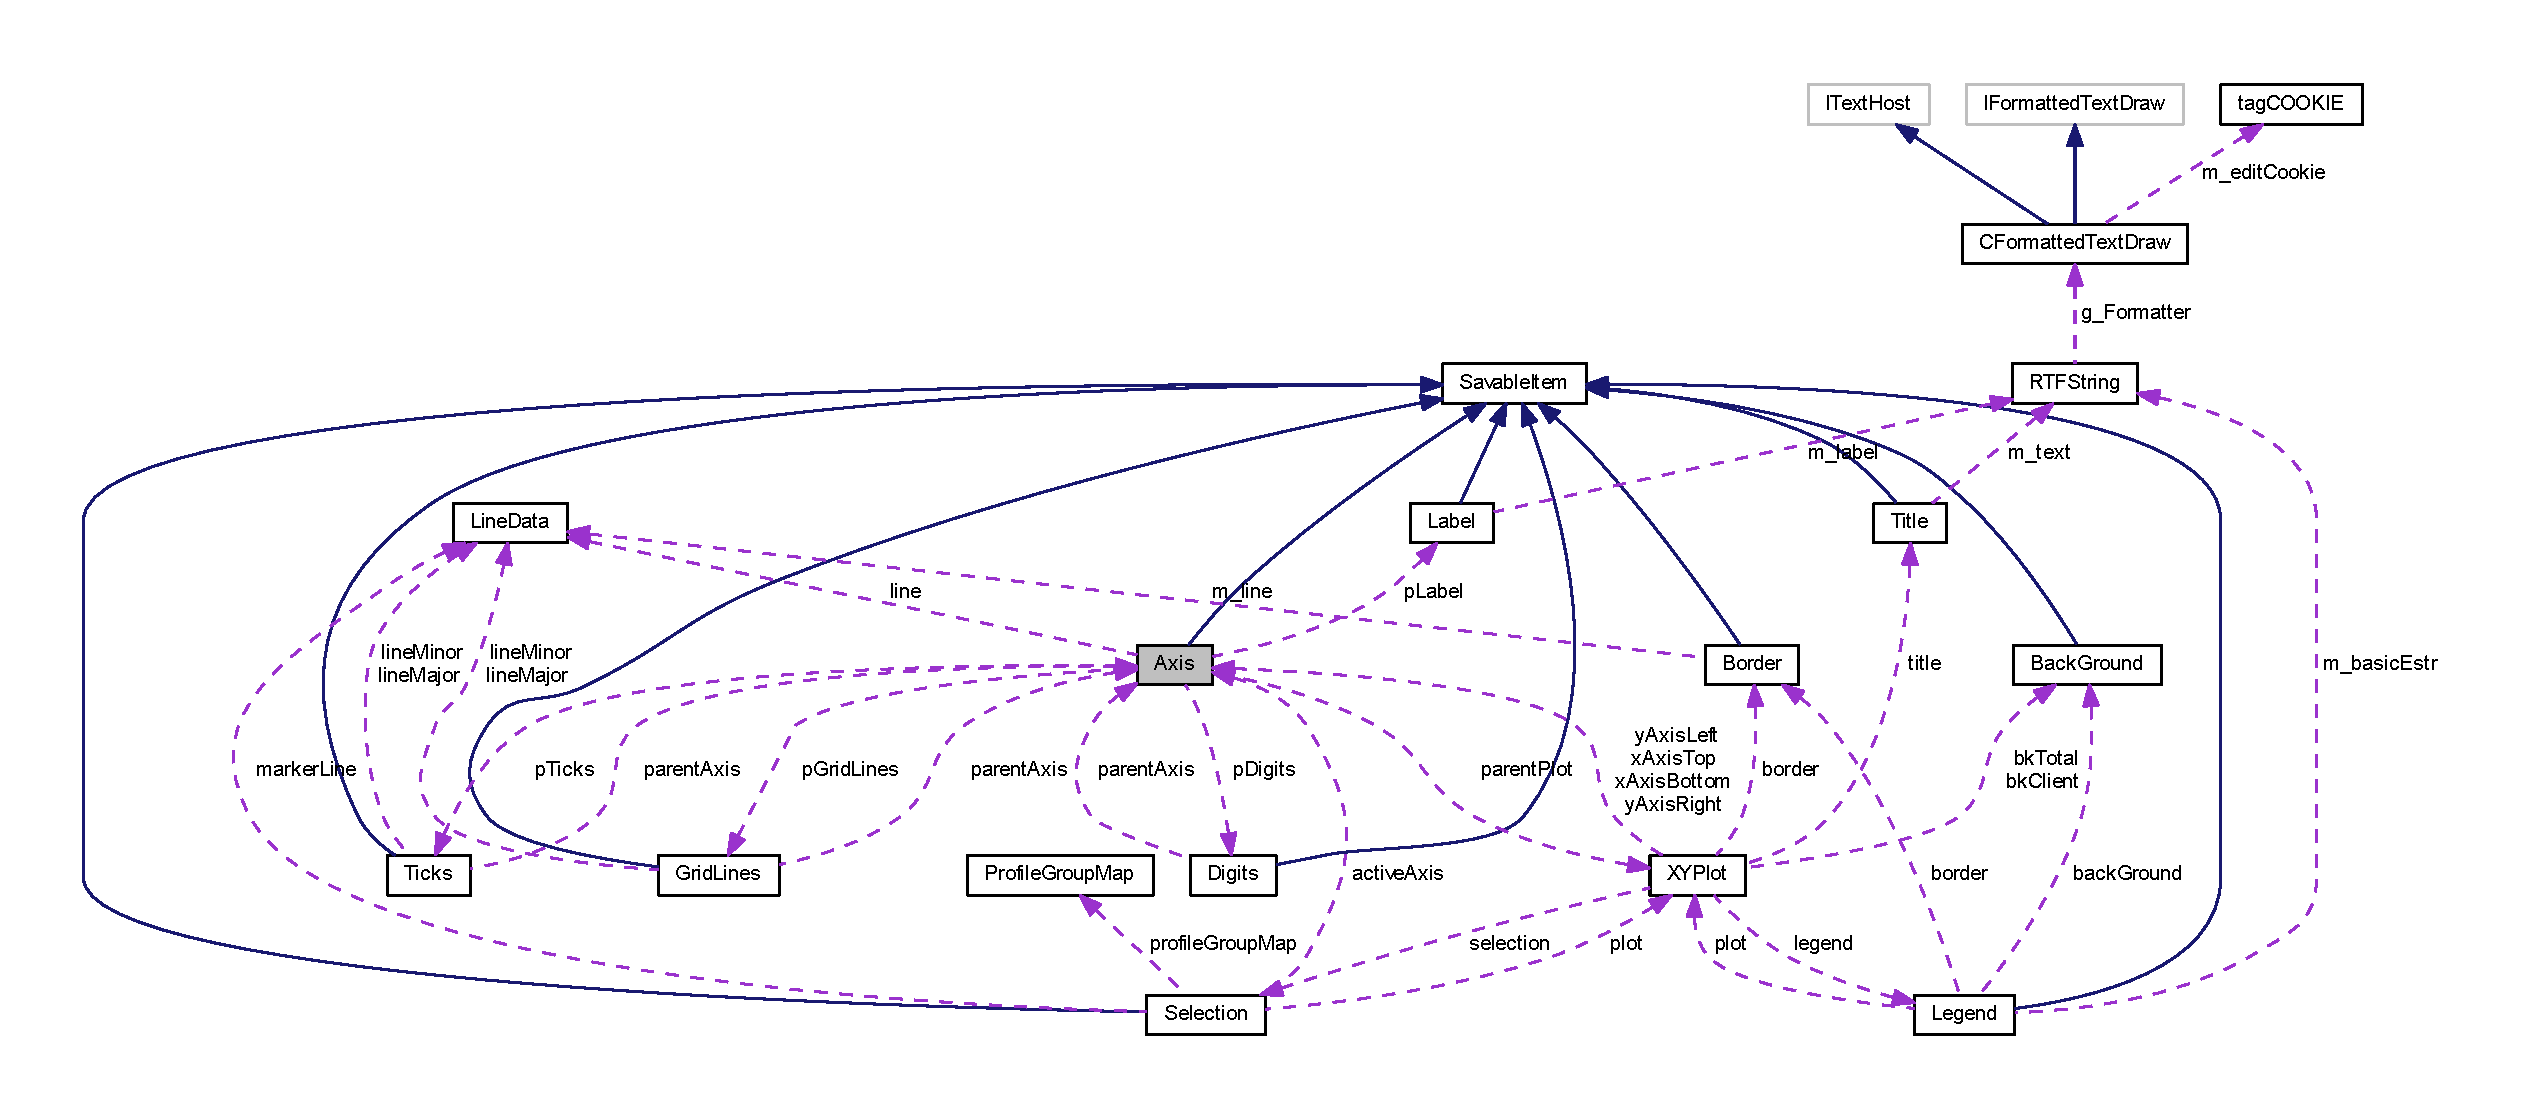
\includegraphics[width=350pt]{class_axis__coll__graph}
\end{center}
\end{figure}
\subsection*{Открытые члены}
\begin{DoxyCompactItemize}
\item 
\hyperlink{class_axis_abd42f819acb0ecb2875d7c5c0f6a90a2}{Axis} (\hyperlink{class_x_y_plot}{X\-Y\-Plot} $\ast$parent)
\item 
virtual \hyperlink{class_axis_a675ffe75a5e61a9e4f60bb79749d5e0c}{$\sim$\-Axis} ()
\item 
B\-O\-O\-L \hyperlink{class_axis_ad51bb24a3f0aa2a15b3d7255a4ad925d}{Create} (\hyperlink{class_x_y_plot}{X\-Y\-Plot} $\ast$\hyperlink{class_axis_a5bb30599723134e0d1250d6028a62575}{parent\-Plot}, int \hyperlink{class_axis_a12acb583f5bf5f386dc0ea78fa4461aa}{id}, unsigned long l\-Styles, const char $\ast$str\-Title=N\-U\-L\-L, double d\-Min=0.\-0, double d\-Max=1.\-0)
\item 
virtual B\-O\-O\-L \hyperlink{class_axis_a895ec09817b379201fe2db2cd1e715aa}{Write} (H\-A\-N\-D\-L\-E h\-File) const 
\item 
virtual B\-O\-O\-L \hyperlink{class_axis_af403dc4181f1681d321f190bd74268ff}{Read} (H\-A\-N\-D\-L\-E h\-File)
\item 
B\-O\-O\-L \hyperlink{class_axis_a5c2b061f2d01872e9cda6e6be0c82f56}{Attach\-Profile} (\hyperlink{class_profile}{Profile} $\ast$prof)
\item 
B\-O\-O\-L \hyperlink{class_axis_a06230b1705046a15a4dddd3252a72691}{Detach\-Profile} (\hyperlink{class_profile}{Profile} $\ast$prof)
\item 
int \hyperlink{class_axis_ab169f9ad45fa8f790e24ee52f7a03996}{Get\-I\-D} () const 
\item 
S\-I\-Z\-E \hyperlink{class_axis_aac35b067fa0786b741627059741e53d3}{Get\-Size} () const 
\item 
int \hyperlink{class_axis_a62a3fedb305053a9cccde8cd34f73637}{Length} () const 
\item 
B\-O\-O\-L \hyperlink{class_axis_a3d3b29ba4d46db3ad1725566e4995e90}{Is\-Time\-History} () const 
\item 
B\-O\-O\-L \hyperlink{class_axis_aea4e6174866d246a5edc2a7b18cf72a4}{Point\-In\-Rect} (const P\-O\-I\-N\-T \&pt)
\item 
\hyperlink{class_line_data}{Line\-Data} \& \hyperlink{class_axis_a37d47434eb57a24e0bee36ac4314edfc}{Get\-Line} ()
\item 
void \hyperlink{class_axis_aa0ddf34c5b437423f1f85c51a54d5239}{Set\-Line} (const \hyperlink{class_line_data}{Line\-Data} \&\hyperlink{class_axis_a68817bcf5ea38ff2d81698175ae9c6ee}{line})
\item 
\hyperlink{class_line_data}{Line\-Data} \& \hyperlink{class_axis_a8500f77c11f6ebef7af8d41050c4f2c1}{Get\-Grid\-Line} (B\-O\-O\-L b\-Major=T\-R\-U\-E)
\item 
void \hyperlink{class_axis_abba8f8d055ffcc6f3a3660d4adb57374}{Set\-Grid\-Line} (const \hyperlink{class_line_data}{Line\-Data} \&\hyperlink{class_axis_a68817bcf5ea38ff2d81698175ae9c6ee}{line}, B\-O\-O\-L b\-Major=T\-R\-U\-E)
\item 
\hyperlink{class_line_data}{Line\-Data} \& \hyperlink{class_axis_a0f12d8e5e59f15a716ef1c2e89b1ff8c}{Get\-Ticks\-Line} (B\-O\-O\-L b\-Major=T\-R\-U\-E)
\item 
void \hyperlink{class_axis_a94241668c2515bf0750cafd53bcb1a42}{Set\-Ticks\-Line} (const \hyperlink{class_line_data}{Line\-Data} \&\hyperlink{class_axis_a68817bcf5ea38ff2d81698175ae9c6ee}{line}, B\-O\-O\-L b\-Major=T\-R\-U\-E)
\item 
D\-W\-O\-R\-D \hyperlink{class_axis_a1b3b93b1d47ab3ca2ec8b906fee6834b}{Set\-Style} (D\-W\-O\-R\-D \hyperlink{class_axis_a9b318f5e15215edb80d3a2bdabc11d44}{dw\-Style}, B\-O\-O\-L b\-Update=T\-R\-U\-E)
\item 
D\-W\-O\-R\-D \hyperlink{class_axis_ac4dc48e8a0ac1cdb24a24f5d45639951}{Modify\-Style} (D\-W\-O\-R\-D \hyperlink{class_axis_a9b318f5e15215edb80d3a2bdabc11d44}{dw\-Style}, B\-O\-O\-L b\-Add=T\-R\-U\-E, B\-O\-O\-L b\-Update=T\-R\-U\-E)
\item 
D\-W\-O\-R\-D \hyperlink{class_axis_a6d6b201a4cce9a6beb8c7055864041ef}{Get\-Style} () const 
\item 
B\-O\-O\-L \hyperlink{class_axis_aaf7ef6cc19a70108d2d86f563b8e822b}{Is\-Auto\-Scaled} () const 
\item 
B\-O\-O\-L \hyperlink{class_axis_a53dc750e1923bf84666d5b7f6c47609e}{Is\-Logarithmic} () const 
\item 
const std\-::vector$<$ P\-O\-I\-N\-T $>$ \& \hyperlink{class_axis_a66f64f1eb719f41512b4ac5cf049a7d2}{Get\-Major\-Ticks\-Pos} () const 
\item 
const std\-::vector$<$ P\-O\-I\-N\-T $>$ \& \hyperlink{class_axis_a4ed3bd789234570a2dfe659dcf0767b0}{Get\-Minor\-Ticks\-Pos} () const 
\item 
const std\-::vector$<$ double $>$ \& \hyperlink{class_axis_a2fe9d0e77dbe887d715d51f88941867f}{Get\-Major\-Ticks\-Values} () const 
\item 
const std\-::vector$<$ double $>$ \& \hyperlink{class_axis_ae278ff239a05ef1d7b76bb37e752dccf}{Get\-Minor\-Ticks\-Values} () const 
\item 
B\-O\-O\-L \hyperlink{class_axis_af51a2bb9da1f6c7e66134f39a22230bf}{Get\-Nearest\-Tick} (double \&val, P\-O\-I\-N\-T \&pt) const 
\item 
const int \hyperlink{class_axis_afa1b9b35e0561aeb36160c9ac1a2cdd9}{Get\-Ticks\-Offset} () const 
\item 
void \hyperlink{class_axis_a9430cb1b9468318b6c05a1c525d74fee}{Set\-Rect} (H\-D\-C h\-D\-C, R\-E\-C\-T rect)
\item 
void \hyperlink{class_axis_a381310504b09d64757c6575ac7cc2568}{Set\-Label} (std\-::string text)
\item 
const std\-::string \& \hyperlink{class_axis_a50eb89d6c720ecaac77d169454b12ed3}{Get\-Label} () const 
\item 
void \hyperlink{class_axis_aa99167d49da06387caa9ce3f53a41b83}{Set\-Label\-Font} (const L\-O\-G\-F\-O\-N\-T $\ast$const plf)
\item 
void \hyperlink{class_axis_adcc942ad32c71008b7f489f235a7a045}{Set\-Label\-Color} (C\-O\-L\-O\-R\-R\-E\-F clr)
\item 
void \hyperlink{class_axis_a6845dc4a3ab9bc86d8a26e195dad3bb6}{Enable\-Label} (B\-O\-O\-L enable)
\item 
B\-O\-O\-L \hyperlink{class_axis_a62b2e2157e201529baeab644300e4086}{Is\-Label\-Enabled} () const 
\item 
void \hyperlink{class_axis_ac82ca2f6125fd9842fc966472b30451b}{Set\-Major\-Ticks\-Length} (int length)
\item 
int \hyperlink{class_axis_a2bdab5744cb822411a9d7b98bea2ebd9}{Get\-Major\-Ticks\-Length} () const 
\item 
void \hyperlink{class_axis_af7612d81af3d140aef6d2c1560f308a7}{Set\-Minor\-Ticks\-Length} (int length)
\item 
int \hyperlink{class_axis_a2b383e7848e4d9284f0b37fcc55c1a5d}{Get\-Minor\-Ticks\-Length} () const 
\item 
void \hyperlink{class_axis_a59d9701163a36d83d19bd8723ced15c0}{Set\-Major\-Ticks\-Count} (int count)
\item 
int \hyperlink{class_axis_a5b56804af56f19924afb2fdaa5002a5e}{Get\-Major\-Ticks\-Count} () const 
\item 
void \hyperlink{class_axis_aaff875d18713ea68dea6375852814a34}{Set\-Minor\-Ticks\-Count} (int count)
\item 
int \hyperlink{class_axis_a8b4b13b1a23c57eb38e195460ecefafc}{Get\-Minor\-Ticks\-Count} () const 
\item 
void \hyperlink{class_axis_a7a6d9bb7ea73f134a7bcdc7839f2fea9}{Enable\-Major\-Ticks} (B\-O\-O\-L enable)
\item 
B\-O\-O\-L \hyperlink{class_axis_a49f99f12afbbe0c3d1feaced4a7ebcc2}{Is\-Major\-Ticks\-Enabled} () const 
\item 
void \hyperlink{class_axis_a51e4e998fdafb039b153824494ec1a64}{Enable\-Minor\-Ticks} (B\-O\-O\-L enable)
\item 
B\-O\-O\-L \hyperlink{class_axis_acb61ef0cfad74adcec76c0c3291fc98f}{Is\-Minor\-Ticks\-Enabled} () const 
\item 
unsigned long \hyperlink{class_axis_a87b08c86575f337d4d09a0b563c76288}{Get\-Ticks\-Style} () const 
\item 
void \hyperlink{class_axis_abbabc70a25f14345308300c67d50e177}{Set\-Ticks\-Style} (unsigned long style)
\item 
void \hyperlink{class_axis_ab23b8dbd121a233ebdabe77122a9c583}{Enable\-Major\-Grid\-Lines} (B\-O\-O\-L enable)
\item 
B\-O\-O\-L \hyperlink{class_axis_a6f037d316ea2e575f8f29fca4beea8ea}{Is\-Major\-Grid\-Lines\-Enabled} () const 
\item 
void \hyperlink{class_axis_a9d36b6a9039e776fa5e91856fd58eb1b}{Enable\-Minor\-Grid\-Lines} (B\-O\-O\-L enable)
\item 
B\-O\-O\-L \hyperlink{class_axis_a46bb27f688cf602a183d0e35e60d3aa8}{Is\-Minor\-Grid\-Lines\-Enabled} () const 
\item 
void \hyperlink{class_axis_a44245d3776209f0010cf91990b171699}{Set\-Digits\-Color} (C\-O\-L\-O\-R\-R\-E\-F color, B\-O\-O\-L b\-Major)
\item 
C\-O\-L\-O\-R\-R\-E\-F \hyperlink{class_axis_a6391e8f6e81eca01de870c0bbaeeb78f}{Get\-Digits\-Color} (B\-O\-O\-L b\-Major) const 
\item 
void \hyperlink{class_axis_aa5baf897c0a1d088ccc673dceba5bb66}{Set\-Digits\-Format} (std\-::string str\-Template, B\-O\-O\-L b\-Major=T\-R\-U\-E)
\item 
const std\-::string \& \hyperlink{class_axis_ad5126fa60e11694e569e382c27d53741}{Get\-Digits\-Format} (B\-O\-O\-L b\-Major=T\-R\-U\-E) const 
\item 
void \hyperlink{class_axis_a710bfe0545ca9ff2053115ca71618a2d}{Set\-Digits\-Font} (const L\-O\-G\-F\-O\-N\-T \&lf, B\-O\-O\-L b\-Major=T\-R\-U\-E)
\item 
void \hyperlink{class_axis_a3381bac80fdd67426366275d1e611877}{Get\-Digits\-Font} (L\-O\-G\-F\-O\-N\-T \&lf, B\-O\-O\-L b\-Major=T\-R\-U\-E) const 
\item 
void \hyperlink{class_axis_ae87d5b9b022bd8c885be4dc460c74a4a}{Enable\-Major\-Digits} (B\-O\-O\-L enable)
\item 
void \hyperlink{class_axis_ab6fc5e053579e7b6d5df8ffcb30a173f}{Enable\-Minor\-Digits} (B\-O\-O\-L enable)
\item 
B\-O\-O\-L \hyperlink{class_axis_ac3ad10e78c202f3d2f2e4c230a3c1fb3}{Is\-Major\-Digits\-Enabled} () const 
\item 
B\-O\-O\-L \hyperlink{class_axis_ab69ae039859200fce16725ea180fb829}{Is\-Minor\-Digits\-Enabled} () const 
\item 
void \hyperlink{class_axis_a41ec122237943357fc410f7e65541642}{Set\-Range} (double d\-Min, double d\-Max)
\item 
void \hyperlink{class_axis_ac64b96cb7b9a98cc4987caf370e1092c}{Get\-Range} (double \&d\-Min, double \&d\-Max) const 
\item 
R\-E\-C\-T \hyperlink{class_axis_a070bb4d5171d26d50a13f195f035476d}{Pre\-Draw} (H\-D\-C h\-D\-C, R\-E\-C\-T rect)
\item 
void \hyperlink{class_axis_a5120d60156ed20854085115bcfcab765}{On\-Draw} (H\-D\-C h\-D\-C)
\item 
void \hyperlink{class_axis_adff2ec412daaec9d055f0129e0a9117f}{Get\-Client\-Rect} (R\-E\-C\-T \&rect) const 
\item 
void \hyperlink{class_axis_a54b571ff70bfca89a515496c0ded3138}{Get\-Limits} (\hyperlink{_coord_converter_8h_aabd54ff6676737c3cae490e3a2363bc4}{L\-P\-A\-X\-I\-S\-L\-I\-M\-I\-T\-S} lpal) const 
\end{DoxyCompactItemize}
\subsection*{Открытые атрибуты}
\begin{DoxyCompactItemize}
\item 
\hyperlink{class_x_y_plot}{X\-Y\-Plot} $\ast$ \hyperlink{class_axis_a5bb30599723134e0d1250d6028a62575}{parent\-Plot}
\end{DoxyCompactItemize}
\subsection*{Защищенные данные}
\begin{DoxyCompactItemize}
\item 
int \hyperlink{class_axis_a12acb583f5bf5f386dc0ea78fa4461aa}{id}
\item 
\hyperlink{class_label}{Label} $\ast$ \hyperlink{class_axis_a28f164cd1a8b77ee7431ade1ee39bc61}{p\-Label}
\item 
\hyperlink{class_line_data}{Line\-Data} \hyperlink{class_axis_a68817bcf5ea38ff2d81698175ae9c6ee}{line}
\item 
\hyperlink{class_ticks}{Ticks} $\ast$ \hyperlink{class_axis_adee9b22eca2aa3d9be3c7a2f9e71039b}{p\-Ticks}
\item 
\hyperlink{class_digits}{Digits} $\ast$ \hyperlink{class_axis_a33bc678ecaf1bda4a3a94c4dab678ac9}{p\-Digits}
\item 
\hyperlink{class_grid_lines}{Grid\-Lines} $\ast$ \hyperlink{class_axis_a56a2fcc5091fd6eca3cd6b80764616bb}{p\-Grid\-Lines}
\item 
double \hyperlink{class_axis_adb0e6da2c0521df03e3e7d820d73af82}{range\-Min}
\item 
double \hyperlink{class_axis_a02853da582831baaa9ebc1289d86ad35}{range\-Max}
\item 
B\-O\-O\-L \hyperlink{class_axis_ae7205720d8bede3b74fab7dd54968d56}{auto\-Scale}
\item 
R\-E\-C\-T \hyperlink{class_axis_a50bf5f208bbca7d528ca52e62b7928e9}{rc\-Self}
\item 
D\-W\-O\-R\-D \hyperlink{class_axis_a9b318f5e15215edb80d3a2bdabc11d44}{dw\-Style}
\item 
std\-::set$<$ \hyperlink{class_profile}{Profile} $\ast$ $>$ \hyperlink{class_axis_a4ce6ac30f1b60e366e6a608b30750d9c}{attached\-Profiles}
\end{DoxyCompactItemize}
\subsection*{Дополнительные унаследованные члены}


\subsection{Конструктор(ы)}
\hypertarget{class_axis_abd42f819acb0ecb2875d7c5c0f6a90a2}{\index{Axis@{Axis}!Axis@{Axis}}
\index{Axis@{Axis}!Axis@{Axis}}
\subsubsection[{Axis}]{\setlength{\rightskip}{0pt plus 5cm}Axis\-::\-Axis (
\begin{DoxyParamCaption}
\item[{{\bf X\-Y\-Plot} $\ast$}]{parent}
\end{DoxyParamCaption}
)}}\label{class_axis_abd42f819acb0ecb2875d7c5c0f6a90a2}
\hypertarget{class_axis_a675ffe75a5e61a9e4f60bb79749d5e0c}{\index{Axis@{Axis}!$\sim$\-Axis@{$\sim$\-Axis}}
\index{$\sim$\-Axis@{$\sim$\-Axis}!Axis@{Axis}}
\subsubsection[{$\sim$\-Axis}]{\setlength{\rightskip}{0pt plus 5cm}Axis\-::$\sim$\-Axis (
\begin{DoxyParamCaption}
\item[{void}]{}
\end{DoxyParamCaption}
)\hspace{0.3cm}{\ttfamily [virtual]}}}\label{class_axis_a675ffe75a5e61a9e4f60bb79749d5e0c}


\subsection{Методы}
\hypertarget{class_axis_a5c2b061f2d01872e9cda6e6be0c82f56}{\index{Axis@{Axis}!Attach\-Profile@{Attach\-Profile}}
\index{Attach\-Profile@{Attach\-Profile}!Axis@{Axis}}
\subsubsection[{Attach\-Profile}]{\setlength{\rightskip}{0pt plus 5cm}B\-O\-O\-L Axis\-::\-Attach\-Profile (
\begin{DoxyParamCaption}
\item[{{\bf Profile} $\ast$}]{prof}
\end{DoxyParamCaption}
)}}\label{class_axis_a5c2b061f2d01872e9cda6e6be0c82f56}
\hypertarget{class_axis_ad51bb24a3f0aa2a15b3d7255a4ad925d}{\index{Axis@{Axis}!Create@{Create}}
\index{Create@{Create}!Axis@{Axis}}
\subsubsection[{Create}]{\setlength{\rightskip}{0pt plus 5cm}B\-O\-O\-L Axis\-::\-Create (
\begin{DoxyParamCaption}
\item[{{\bf X\-Y\-Plot} $\ast$}]{parent\-Plot, }
\item[{int}]{id, }
\item[{unsigned long}]{l\-Styles, }
\item[{const char $\ast$}]{str\-Title = {\ttfamily NULL}, }
\item[{double}]{d\-Min = {\ttfamily 0.0}, }
\item[{double}]{d\-Max = {\ttfamily 1.0}}
\end{DoxyParamCaption}
)}}\label{class_axis_ad51bb24a3f0aa2a15b3d7255a4ad925d}
\hypertarget{class_axis_a06230b1705046a15a4dddd3252a72691}{\index{Axis@{Axis}!Detach\-Profile@{Detach\-Profile}}
\index{Detach\-Profile@{Detach\-Profile}!Axis@{Axis}}
\subsubsection[{Detach\-Profile}]{\setlength{\rightskip}{0pt plus 5cm}B\-O\-O\-L Axis\-::\-Detach\-Profile (
\begin{DoxyParamCaption}
\item[{{\bf Profile} $\ast$}]{prof}
\end{DoxyParamCaption}
)}}\label{class_axis_a06230b1705046a15a4dddd3252a72691}
\hypertarget{class_axis_a6845dc4a3ab9bc86d8a26e195dad3bb6}{\index{Axis@{Axis}!Enable\-Label@{Enable\-Label}}
\index{Enable\-Label@{Enable\-Label}!Axis@{Axis}}
\subsubsection[{Enable\-Label}]{\setlength{\rightskip}{0pt plus 5cm}void Axis\-::\-Enable\-Label (
\begin{DoxyParamCaption}
\item[{B\-O\-O\-L}]{enable}
\end{DoxyParamCaption}
)\hspace{0.3cm}{\ttfamily [inline]}}}\label{class_axis_a6845dc4a3ab9bc86d8a26e195dad3bb6}
\hypertarget{class_axis_ae87d5b9b022bd8c885be4dc460c74a4a}{\index{Axis@{Axis}!Enable\-Major\-Digits@{Enable\-Major\-Digits}}
\index{Enable\-Major\-Digits@{Enable\-Major\-Digits}!Axis@{Axis}}
\subsubsection[{Enable\-Major\-Digits}]{\setlength{\rightskip}{0pt plus 5cm}void Axis\-::\-Enable\-Major\-Digits (
\begin{DoxyParamCaption}
\item[{B\-O\-O\-L}]{enable}
\end{DoxyParamCaption}
)\hspace{0.3cm}{\ttfamily [inline]}}}\label{class_axis_ae87d5b9b022bd8c885be4dc460c74a4a}
\hypertarget{class_axis_ab23b8dbd121a233ebdabe77122a9c583}{\index{Axis@{Axis}!Enable\-Major\-Grid\-Lines@{Enable\-Major\-Grid\-Lines}}
\index{Enable\-Major\-Grid\-Lines@{Enable\-Major\-Grid\-Lines}!Axis@{Axis}}
\subsubsection[{Enable\-Major\-Grid\-Lines}]{\setlength{\rightskip}{0pt plus 5cm}void Axis\-::\-Enable\-Major\-Grid\-Lines (
\begin{DoxyParamCaption}
\item[{B\-O\-O\-L}]{enable}
\end{DoxyParamCaption}
)\hspace{0.3cm}{\ttfamily [inline]}}}\label{class_axis_ab23b8dbd121a233ebdabe77122a9c583}
\hypertarget{class_axis_a7a6d9bb7ea73f134a7bcdc7839f2fea9}{\index{Axis@{Axis}!Enable\-Major\-Ticks@{Enable\-Major\-Ticks}}
\index{Enable\-Major\-Ticks@{Enable\-Major\-Ticks}!Axis@{Axis}}
\subsubsection[{Enable\-Major\-Ticks}]{\setlength{\rightskip}{0pt plus 5cm}void Axis\-::\-Enable\-Major\-Ticks (
\begin{DoxyParamCaption}
\item[{B\-O\-O\-L}]{enable}
\end{DoxyParamCaption}
)\hspace{0.3cm}{\ttfamily [inline]}}}\label{class_axis_a7a6d9bb7ea73f134a7bcdc7839f2fea9}
\hypertarget{class_axis_ab6fc5e053579e7b6d5df8ffcb30a173f}{\index{Axis@{Axis}!Enable\-Minor\-Digits@{Enable\-Minor\-Digits}}
\index{Enable\-Minor\-Digits@{Enable\-Minor\-Digits}!Axis@{Axis}}
\subsubsection[{Enable\-Minor\-Digits}]{\setlength{\rightskip}{0pt plus 5cm}void Axis\-::\-Enable\-Minor\-Digits (
\begin{DoxyParamCaption}
\item[{B\-O\-O\-L}]{enable}
\end{DoxyParamCaption}
)\hspace{0.3cm}{\ttfamily [inline]}}}\label{class_axis_ab6fc5e053579e7b6d5df8ffcb30a173f}
\hypertarget{class_axis_a9d36b6a9039e776fa5e91856fd58eb1b}{\index{Axis@{Axis}!Enable\-Minor\-Grid\-Lines@{Enable\-Minor\-Grid\-Lines}}
\index{Enable\-Minor\-Grid\-Lines@{Enable\-Minor\-Grid\-Lines}!Axis@{Axis}}
\subsubsection[{Enable\-Minor\-Grid\-Lines}]{\setlength{\rightskip}{0pt plus 5cm}void Axis\-::\-Enable\-Minor\-Grid\-Lines (
\begin{DoxyParamCaption}
\item[{B\-O\-O\-L}]{enable}
\end{DoxyParamCaption}
)\hspace{0.3cm}{\ttfamily [inline]}}}\label{class_axis_a9d36b6a9039e776fa5e91856fd58eb1b}
\hypertarget{class_axis_a51e4e998fdafb039b153824494ec1a64}{\index{Axis@{Axis}!Enable\-Minor\-Ticks@{Enable\-Minor\-Ticks}}
\index{Enable\-Minor\-Ticks@{Enable\-Minor\-Ticks}!Axis@{Axis}}
\subsubsection[{Enable\-Minor\-Ticks}]{\setlength{\rightskip}{0pt plus 5cm}void Axis\-::\-Enable\-Minor\-Ticks (
\begin{DoxyParamCaption}
\item[{B\-O\-O\-L}]{enable}
\end{DoxyParamCaption}
)\hspace{0.3cm}{\ttfamily [inline]}}}\label{class_axis_a51e4e998fdafb039b153824494ec1a64}
\hypertarget{class_axis_adff2ec412daaec9d055f0129e0a9117f}{\index{Axis@{Axis}!Get\-Client\-Rect@{Get\-Client\-Rect}}
\index{Get\-Client\-Rect@{Get\-Client\-Rect}!Axis@{Axis}}
\subsubsection[{Get\-Client\-Rect}]{\setlength{\rightskip}{0pt plus 5cm}void Axis\-::\-Get\-Client\-Rect (
\begin{DoxyParamCaption}
\item[{R\-E\-C\-T \&}]{rect}
\end{DoxyParamCaption}
) const}}\label{class_axis_adff2ec412daaec9d055f0129e0a9117f}
\hypertarget{class_axis_a6391e8f6e81eca01de870c0bbaeeb78f}{\index{Axis@{Axis}!Get\-Digits\-Color@{Get\-Digits\-Color}}
\index{Get\-Digits\-Color@{Get\-Digits\-Color}!Axis@{Axis}}
\subsubsection[{Get\-Digits\-Color}]{\setlength{\rightskip}{0pt plus 5cm}C\-O\-L\-O\-R\-R\-E\-F Axis\-::\-Get\-Digits\-Color (
\begin{DoxyParamCaption}
\item[{B\-O\-O\-L}]{b\-Major}
\end{DoxyParamCaption}
) const\hspace{0.3cm}{\ttfamily [inline]}}}\label{class_axis_a6391e8f6e81eca01de870c0bbaeeb78f}
\hypertarget{class_axis_a3381bac80fdd67426366275d1e611877}{\index{Axis@{Axis}!Get\-Digits\-Font@{Get\-Digits\-Font}}
\index{Get\-Digits\-Font@{Get\-Digits\-Font}!Axis@{Axis}}
\subsubsection[{Get\-Digits\-Font}]{\setlength{\rightskip}{0pt plus 5cm}void Axis\-::\-Get\-Digits\-Font (
\begin{DoxyParamCaption}
\item[{L\-O\-G\-F\-O\-N\-T \&}]{lf, }
\item[{B\-O\-O\-L}]{b\-Major = {\ttfamily TRUE}}
\end{DoxyParamCaption}
) const\hspace{0.3cm}{\ttfamily [inline]}}}\label{class_axis_a3381bac80fdd67426366275d1e611877}
\hypertarget{class_axis_ad5126fa60e11694e569e382c27d53741}{\index{Axis@{Axis}!Get\-Digits\-Format@{Get\-Digits\-Format}}
\index{Get\-Digits\-Format@{Get\-Digits\-Format}!Axis@{Axis}}
\subsubsection[{Get\-Digits\-Format}]{\setlength{\rightskip}{0pt plus 5cm}const std\-::string\& Axis\-::\-Get\-Digits\-Format (
\begin{DoxyParamCaption}
\item[{B\-O\-O\-L}]{b\-Major = {\ttfamily TRUE}}
\end{DoxyParamCaption}
) const\hspace{0.3cm}{\ttfamily [inline]}}}\label{class_axis_ad5126fa60e11694e569e382c27d53741}
\hypertarget{class_axis_a8500f77c11f6ebef7af8d41050c4f2c1}{\index{Axis@{Axis}!Get\-Grid\-Line@{Get\-Grid\-Line}}
\index{Get\-Grid\-Line@{Get\-Grid\-Line}!Axis@{Axis}}
\subsubsection[{Get\-Grid\-Line}]{\setlength{\rightskip}{0pt plus 5cm}{\bf Line\-Data}\& Axis\-::\-Get\-Grid\-Line (
\begin{DoxyParamCaption}
\item[{B\-O\-O\-L}]{b\-Major = {\ttfamily TRUE}}
\end{DoxyParamCaption}
)\hspace{0.3cm}{\ttfamily [inline]}}}\label{class_axis_a8500f77c11f6ebef7af8d41050c4f2c1}
\hypertarget{class_axis_ab169f9ad45fa8f790e24ee52f7a03996}{\index{Axis@{Axis}!Get\-I\-D@{Get\-I\-D}}
\index{Get\-I\-D@{Get\-I\-D}!Axis@{Axis}}
\subsubsection[{Get\-I\-D}]{\setlength{\rightskip}{0pt plus 5cm}int Axis\-::\-Get\-I\-D (
\begin{DoxyParamCaption}
{}
\end{DoxyParamCaption}
) const\hspace{0.3cm}{\ttfamily [inline]}}}\label{class_axis_ab169f9ad45fa8f790e24ee52f7a03996}
\hypertarget{class_axis_a50eb89d6c720ecaac77d169454b12ed3}{\index{Axis@{Axis}!Get\-Label@{Get\-Label}}
\index{Get\-Label@{Get\-Label}!Axis@{Axis}}
\subsubsection[{Get\-Label}]{\setlength{\rightskip}{0pt plus 5cm}const std\-::string\& Axis\-::\-Get\-Label (
\begin{DoxyParamCaption}
{}
\end{DoxyParamCaption}
) const\hspace{0.3cm}{\ttfamily [inline]}}}\label{class_axis_a50eb89d6c720ecaac77d169454b12ed3}
\hypertarget{class_axis_a54b571ff70bfca89a515496c0ded3138}{\index{Axis@{Axis}!Get\-Limits@{Get\-Limits}}
\index{Get\-Limits@{Get\-Limits}!Axis@{Axis}}
\subsubsection[{Get\-Limits}]{\setlength{\rightskip}{0pt plus 5cm}void Axis\-::\-Get\-Limits (
\begin{DoxyParamCaption}
\item[{{\bf L\-P\-A\-X\-I\-S\-L\-I\-M\-I\-T\-S}}]{lpal}
\end{DoxyParamCaption}
) const}}\label{class_axis_a54b571ff70bfca89a515496c0ded3138}
\hypertarget{class_axis_a37d47434eb57a24e0bee36ac4314edfc}{\index{Axis@{Axis}!Get\-Line@{Get\-Line}}
\index{Get\-Line@{Get\-Line}!Axis@{Axis}}
\subsubsection[{Get\-Line}]{\setlength{\rightskip}{0pt plus 5cm}{\bf Line\-Data}\& Axis\-::\-Get\-Line (
\begin{DoxyParamCaption}
{}
\end{DoxyParamCaption}
)\hspace{0.3cm}{\ttfamily [inline]}}}\label{class_axis_a37d47434eb57a24e0bee36ac4314edfc}
\hypertarget{class_axis_a5b56804af56f19924afb2fdaa5002a5e}{\index{Axis@{Axis}!Get\-Major\-Ticks\-Count@{Get\-Major\-Ticks\-Count}}
\index{Get\-Major\-Ticks\-Count@{Get\-Major\-Ticks\-Count}!Axis@{Axis}}
\subsubsection[{Get\-Major\-Ticks\-Count}]{\setlength{\rightskip}{0pt plus 5cm}int Axis\-::\-Get\-Major\-Ticks\-Count (
\begin{DoxyParamCaption}
{}
\end{DoxyParamCaption}
) const\hspace{0.3cm}{\ttfamily [inline]}}}\label{class_axis_a5b56804af56f19924afb2fdaa5002a5e}
\hypertarget{class_axis_a2bdab5744cb822411a9d7b98bea2ebd9}{\index{Axis@{Axis}!Get\-Major\-Ticks\-Length@{Get\-Major\-Ticks\-Length}}
\index{Get\-Major\-Ticks\-Length@{Get\-Major\-Ticks\-Length}!Axis@{Axis}}
\subsubsection[{Get\-Major\-Ticks\-Length}]{\setlength{\rightskip}{0pt plus 5cm}int Axis\-::\-Get\-Major\-Ticks\-Length (
\begin{DoxyParamCaption}
{}
\end{DoxyParamCaption}
) const\hspace{0.3cm}{\ttfamily [inline]}}}\label{class_axis_a2bdab5744cb822411a9d7b98bea2ebd9}
\hypertarget{class_axis_a66f64f1eb719f41512b4ac5cf049a7d2}{\index{Axis@{Axis}!Get\-Major\-Ticks\-Pos@{Get\-Major\-Ticks\-Pos}}
\index{Get\-Major\-Ticks\-Pos@{Get\-Major\-Ticks\-Pos}!Axis@{Axis}}
\subsubsection[{Get\-Major\-Ticks\-Pos}]{\setlength{\rightskip}{0pt plus 5cm}const std\-::vector$<$P\-O\-I\-N\-T$>$\& Axis\-::\-Get\-Major\-Ticks\-Pos (
\begin{DoxyParamCaption}
{}
\end{DoxyParamCaption}
) const\hspace{0.3cm}{\ttfamily [inline]}}}\label{class_axis_a66f64f1eb719f41512b4ac5cf049a7d2}
\hypertarget{class_axis_a2fe9d0e77dbe887d715d51f88941867f}{\index{Axis@{Axis}!Get\-Major\-Ticks\-Values@{Get\-Major\-Ticks\-Values}}
\index{Get\-Major\-Ticks\-Values@{Get\-Major\-Ticks\-Values}!Axis@{Axis}}
\subsubsection[{Get\-Major\-Ticks\-Values}]{\setlength{\rightskip}{0pt plus 5cm}const std\-::vector$<$double$>$\& Axis\-::\-Get\-Major\-Ticks\-Values (
\begin{DoxyParamCaption}
{}
\end{DoxyParamCaption}
) const\hspace{0.3cm}{\ttfamily [inline]}}}\label{class_axis_a2fe9d0e77dbe887d715d51f88941867f}
\hypertarget{class_axis_a8b4b13b1a23c57eb38e195460ecefafc}{\index{Axis@{Axis}!Get\-Minor\-Ticks\-Count@{Get\-Minor\-Ticks\-Count}}
\index{Get\-Minor\-Ticks\-Count@{Get\-Minor\-Ticks\-Count}!Axis@{Axis}}
\subsubsection[{Get\-Minor\-Ticks\-Count}]{\setlength{\rightskip}{0pt plus 5cm}int Axis\-::\-Get\-Minor\-Ticks\-Count (
\begin{DoxyParamCaption}
{}
\end{DoxyParamCaption}
) const\hspace{0.3cm}{\ttfamily [inline]}}}\label{class_axis_a8b4b13b1a23c57eb38e195460ecefafc}
\hypertarget{class_axis_a2b383e7848e4d9284f0b37fcc55c1a5d}{\index{Axis@{Axis}!Get\-Minor\-Ticks\-Length@{Get\-Minor\-Ticks\-Length}}
\index{Get\-Minor\-Ticks\-Length@{Get\-Minor\-Ticks\-Length}!Axis@{Axis}}
\subsubsection[{Get\-Minor\-Ticks\-Length}]{\setlength{\rightskip}{0pt plus 5cm}int Axis\-::\-Get\-Minor\-Ticks\-Length (
\begin{DoxyParamCaption}
{}
\end{DoxyParamCaption}
) const\hspace{0.3cm}{\ttfamily [inline]}}}\label{class_axis_a2b383e7848e4d9284f0b37fcc55c1a5d}
\hypertarget{class_axis_a4ed3bd789234570a2dfe659dcf0767b0}{\index{Axis@{Axis}!Get\-Minor\-Ticks\-Pos@{Get\-Minor\-Ticks\-Pos}}
\index{Get\-Minor\-Ticks\-Pos@{Get\-Minor\-Ticks\-Pos}!Axis@{Axis}}
\subsubsection[{Get\-Minor\-Ticks\-Pos}]{\setlength{\rightskip}{0pt plus 5cm}const std\-::vector$<$P\-O\-I\-N\-T$>$\& Axis\-::\-Get\-Minor\-Ticks\-Pos (
\begin{DoxyParamCaption}
{}
\end{DoxyParamCaption}
) const\hspace{0.3cm}{\ttfamily [inline]}}}\label{class_axis_a4ed3bd789234570a2dfe659dcf0767b0}
\hypertarget{class_axis_ae278ff239a05ef1d7b76bb37e752dccf}{\index{Axis@{Axis}!Get\-Minor\-Ticks\-Values@{Get\-Minor\-Ticks\-Values}}
\index{Get\-Minor\-Ticks\-Values@{Get\-Minor\-Ticks\-Values}!Axis@{Axis}}
\subsubsection[{Get\-Minor\-Ticks\-Values}]{\setlength{\rightskip}{0pt plus 5cm}const std\-::vector$<$double$>$\& Axis\-::\-Get\-Minor\-Ticks\-Values (
\begin{DoxyParamCaption}
{}
\end{DoxyParamCaption}
) const\hspace{0.3cm}{\ttfamily [inline]}}}\label{class_axis_ae278ff239a05ef1d7b76bb37e752dccf}
\hypertarget{class_axis_af51a2bb9da1f6c7e66134f39a22230bf}{\index{Axis@{Axis}!Get\-Nearest\-Tick@{Get\-Nearest\-Tick}}
\index{Get\-Nearest\-Tick@{Get\-Nearest\-Tick}!Axis@{Axis}}
\subsubsection[{Get\-Nearest\-Tick}]{\setlength{\rightskip}{0pt plus 5cm}B\-O\-O\-L Axis\-::\-Get\-Nearest\-Tick (
\begin{DoxyParamCaption}
\item[{double \&}]{val, }
\item[{P\-O\-I\-N\-T \&}]{pt}
\end{DoxyParamCaption}
) const\hspace{0.3cm}{\ttfamily [inline]}}}\label{class_axis_af51a2bb9da1f6c7e66134f39a22230bf}
\hypertarget{class_axis_ac64b96cb7b9a98cc4987caf370e1092c}{\index{Axis@{Axis}!Get\-Range@{Get\-Range}}
\index{Get\-Range@{Get\-Range}!Axis@{Axis}}
\subsubsection[{Get\-Range}]{\setlength{\rightskip}{0pt plus 5cm}void Axis\-::\-Get\-Range (
\begin{DoxyParamCaption}
\item[{double \&}]{d\-Min, }
\item[{double \&}]{d\-Max}
\end{DoxyParamCaption}
) const\hspace{0.3cm}{\ttfamily [inline]}}}\label{class_axis_ac64b96cb7b9a98cc4987caf370e1092c}
\hypertarget{class_axis_aac35b067fa0786b741627059741e53d3}{\index{Axis@{Axis}!Get\-Size@{Get\-Size}}
\index{Get\-Size@{Get\-Size}!Axis@{Axis}}
\subsubsection[{Get\-Size}]{\setlength{\rightskip}{0pt plus 5cm}S\-I\-Z\-E Axis\-::\-Get\-Size (
\begin{DoxyParamCaption}
{}
\end{DoxyParamCaption}
) const}}\label{class_axis_aac35b067fa0786b741627059741e53d3}
\hypertarget{class_axis_a6d6b201a4cce9a6beb8c7055864041ef}{\index{Axis@{Axis}!Get\-Style@{Get\-Style}}
\index{Get\-Style@{Get\-Style}!Axis@{Axis}}
\subsubsection[{Get\-Style}]{\setlength{\rightskip}{0pt plus 5cm}D\-W\-O\-R\-D Axis\-::\-Get\-Style (
\begin{DoxyParamCaption}
{}
\end{DoxyParamCaption}
) const\hspace{0.3cm}{\ttfamily [inline]}}}\label{class_axis_a6d6b201a4cce9a6beb8c7055864041ef}
\hypertarget{class_axis_a0f12d8e5e59f15a716ef1c2e89b1ff8c}{\index{Axis@{Axis}!Get\-Ticks\-Line@{Get\-Ticks\-Line}}
\index{Get\-Ticks\-Line@{Get\-Ticks\-Line}!Axis@{Axis}}
\subsubsection[{Get\-Ticks\-Line}]{\setlength{\rightskip}{0pt plus 5cm}{\bf Line\-Data}\& Axis\-::\-Get\-Ticks\-Line (
\begin{DoxyParamCaption}
\item[{B\-O\-O\-L}]{b\-Major = {\ttfamily TRUE}}
\end{DoxyParamCaption}
)\hspace{0.3cm}{\ttfamily [inline]}}}\label{class_axis_a0f12d8e5e59f15a716ef1c2e89b1ff8c}
\hypertarget{class_axis_afa1b9b35e0561aeb36160c9ac1a2cdd9}{\index{Axis@{Axis}!Get\-Ticks\-Offset@{Get\-Ticks\-Offset}}
\index{Get\-Ticks\-Offset@{Get\-Ticks\-Offset}!Axis@{Axis}}
\subsubsection[{Get\-Ticks\-Offset}]{\setlength{\rightskip}{0pt plus 5cm}const int Axis\-::\-Get\-Ticks\-Offset (
\begin{DoxyParamCaption}
{}
\end{DoxyParamCaption}
) const\hspace{0.3cm}{\ttfamily [inline]}}}\label{class_axis_afa1b9b35e0561aeb36160c9ac1a2cdd9}
\hypertarget{class_axis_a87b08c86575f337d4d09a0b563c76288}{\index{Axis@{Axis}!Get\-Ticks\-Style@{Get\-Ticks\-Style}}
\index{Get\-Ticks\-Style@{Get\-Ticks\-Style}!Axis@{Axis}}
\subsubsection[{Get\-Ticks\-Style}]{\setlength{\rightskip}{0pt plus 5cm}unsigned long Axis\-::\-Get\-Ticks\-Style (
\begin{DoxyParamCaption}
{}
\end{DoxyParamCaption}
) const\hspace{0.3cm}{\ttfamily [inline]}}}\label{class_axis_a87b08c86575f337d4d09a0b563c76288}
\hypertarget{class_axis_aaf7ef6cc19a70108d2d86f563b8e822b}{\index{Axis@{Axis}!Is\-Auto\-Scaled@{Is\-Auto\-Scaled}}
\index{Is\-Auto\-Scaled@{Is\-Auto\-Scaled}!Axis@{Axis}}
\subsubsection[{Is\-Auto\-Scaled}]{\setlength{\rightskip}{0pt plus 5cm}B\-O\-O\-L Axis\-::\-Is\-Auto\-Scaled (
\begin{DoxyParamCaption}
{}
\end{DoxyParamCaption}
) const\hspace{0.3cm}{\ttfamily [inline]}}}\label{class_axis_aaf7ef6cc19a70108d2d86f563b8e822b}
\hypertarget{class_axis_a62b2e2157e201529baeab644300e4086}{\index{Axis@{Axis}!Is\-Label\-Enabled@{Is\-Label\-Enabled}}
\index{Is\-Label\-Enabled@{Is\-Label\-Enabled}!Axis@{Axis}}
\subsubsection[{Is\-Label\-Enabled}]{\setlength{\rightskip}{0pt plus 5cm}B\-O\-O\-L Axis\-::\-Is\-Label\-Enabled (
\begin{DoxyParamCaption}
{}
\end{DoxyParamCaption}
) const\hspace{0.3cm}{\ttfamily [inline]}}}\label{class_axis_a62b2e2157e201529baeab644300e4086}
\hypertarget{class_axis_a53dc750e1923bf84666d5b7f6c47609e}{\index{Axis@{Axis}!Is\-Logarithmic@{Is\-Logarithmic}}
\index{Is\-Logarithmic@{Is\-Logarithmic}!Axis@{Axis}}
\subsubsection[{Is\-Logarithmic}]{\setlength{\rightskip}{0pt plus 5cm}B\-O\-O\-L Axis\-::\-Is\-Logarithmic (
\begin{DoxyParamCaption}
{}
\end{DoxyParamCaption}
) const\hspace{0.3cm}{\ttfamily [inline]}}}\label{class_axis_a53dc750e1923bf84666d5b7f6c47609e}
\hypertarget{class_axis_ac3ad10e78c202f3d2f2e4c230a3c1fb3}{\index{Axis@{Axis}!Is\-Major\-Digits\-Enabled@{Is\-Major\-Digits\-Enabled}}
\index{Is\-Major\-Digits\-Enabled@{Is\-Major\-Digits\-Enabled}!Axis@{Axis}}
\subsubsection[{Is\-Major\-Digits\-Enabled}]{\setlength{\rightskip}{0pt plus 5cm}B\-O\-O\-L Axis\-::\-Is\-Major\-Digits\-Enabled (
\begin{DoxyParamCaption}
{}
\end{DoxyParamCaption}
) const\hspace{0.3cm}{\ttfamily [inline]}}}\label{class_axis_ac3ad10e78c202f3d2f2e4c230a3c1fb3}
\hypertarget{class_axis_a6f037d316ea2e575f8f29fca4beea8ea}{\index{Axis@{Axis}!Is\-Major\-Grid\-Lines\-Enabled@{Is\-Major\-Grid\-Lines\-Enabled}}
\index{Is\-Major\-Grid\-Lines\-Enabled@{Is\-Major\-Grid\-Lines\-Enabled}!Axis@{Axis}}
\subsubsection[{Is\-Major\-Grid\-Lines\-Enabled}]{\setlength{\rightskip}{0pt plus 5cm}B\-O\-O\-L Axis\-::\-Is\-Major\-Grid\-Lines\-Enabled (
\begin{DoxyParamCaption}
{}
\end{DoxyParamCaption}
) const\hspace{0.3cm}{\ttfamily [inline]}}}\label{class_axis_a6f037d316ea2e575f8f29fca4beea8ea}
\hypertarget{class_axis_a49f99f12afbbe0c3d1feaced4a7ebcc2}{\index{Axis@{Axis}!Is\-Major\-Ticks\-Enabled@{Is\-Major\-Ticks\-Enabled}}
\index{Is\-Major\-Ticks\-Enabled@{Is\-Major\-Ticks\-Enabled}!Axis@{Axis}}
\subsubsection[{Is\-Major\-Ticks\-Enabled}]{\setlength{\rightskip}{0pt plus 5cm}B\-O\-O\-L Axis\-::\-Is\-Major\-Ticks\-Enabled (
\begin{DoxyParamCaption}
{}
\end{DoxyParamCaption}
) const\hspace{0.3cm}{\ttfamily [inline]}}}\label{class_axis_a49f99f12afbbe0c3d1feaced4a7ebcc2}
\hypertarget{class_axis_ab69ae039859200fce16725ea180fb829}{\index{Axis@{Axis}!Is\-Minor\-Digits\-Enabled@{Is\-Minor\-Digits\-Enabled}}
\index{Is\-Minor\-Digits\-Enabled@{Is\-Minor\-Digits\-Enabled}!Axis@{Axis}}
\subsubsection[{Is\-Minor\-Digits\-Enabled}]{\setlength{\rightskip}{0pt plus 5cm}B\-O\-O\-L Axis\-::\-Is\-Minor\-Digits\-Enabled (
\begin{DoxyParamCaption}
{}
\end{DoxyParamCaption}
) const\hspace{0.3cm}{\ttfamily [inline]}}}\label{class_axis_ab69ae039859200fce16725ea180fb829}
\hypertarget{class_axis_a46bb27f688cf602a183d0e35e60d3aa8}{\index{Axis@{Axis}!Is\-Minor\-Grid\-Lines\-Enabled@{Is\-Minor\-Grid\-Lines\-Enabled}}
\index{Is\-Minor\-Grid\-Lines\-Enabled@{Is\-Minor\-Grid\-Lines\-Enabled}!Axis@{Axis}}
\subsubsection[{Is\-Minor\-Grid\-Lines\-Enabled}]{\setlength{\rightskip}{0pt plus 5cm}B\-O\-O\-L Axis\-::\-Is\-Minor\-Grid\-Lines\-Enabled (
\begin{DoxyParamCaption}
{}
\end{DoxyParamCaption}
) const\hspace{0.3cm}{\ttfamily [inline]}}}\label{class_axis_a46bb27f688cf602a183d0e35e60d3aa8}
\hypertarget{class_axis_acb61ef0cfad74adcec76c0c3291fc98f}{\index{Axis@{Axis}!Is\-Minor\-Ticks\-Enabled@{Is\-Minor\-Ticks\-Enabled}}
\index{Is\-Minor\-Ticks\-Enabled@{Is\-Minor\-Ticks\-Enabled}!Axis@{Axis}}
\subsubsection[{Is\-Minor\-Ticks\-Enabled}]{\setlength{\rightskip}{0pt plus 5cm}B\-O\-O\-L Axis\-::\-Is\-Minor\-Ticks\-Enabled (
\begin{DoxyParamCaption}
{}
\end{DoxyParamCaption}
) const\hspace{0.3cm}{\ttfamily [inline]}}}\label{class_axis_acb61ef0cfad74adcec76c0c3291fc98f}
\hypertarget{class_axis_a3d3b29ba4d46db3ad1725566e4995e90}{\index{Axis@{Axis}!Is\-Time\-History@{Is\-Time\-History}}
\index{Is\-Time\-History@{Is\-Time\-History}!Axis@{Axis}}
\subsubsection[{Is\-Time\-History}]{\setlength{\rightskip}{0pt plus 5cm}B\-O\-O\-L Axis\-::\-Is\-Time\-History (
\begin{DoxyParamCaption}
{}
\end{DoxyParamCaption}
) const\hspace{0.3cm}{\ttfamily [inline]}}}\label{class_axis_a3d3b29ba4d46db3ad1725566e4995e90}
\hypertarget{class_axis_a62a3fedb305053a9cccde8cd34f73637}{\index{Axis@{Axis}!Length@{Length}}
\index{Length@{Length}!Axis@{Axis}}
\subsubsection[{Length}]{\setlength{\rightskip}{0pt plus 5cm}int Axis\-::\-Length (
\begin{DoxyParamCaption}
{}
\end{DoxyParamCaption}
) const}}\label{class_axis_a62a3fedb305053a9cccde8cd34f73637}
\hypertarget{class_axis_ac4dc48e8a0ac1cdb24a24f5d45639951}{\index{Axis@{Axis}!Modify\-Style@{Modify\-Style}}
\index{Modify\-Style@{Modify\-Style}!Axis@{Axis}}
\subsubsection[{Modify\-Style}]{\setlength{\rightskip}{0pt plus 5cm}D\-W\-O\-R\-D Axis\-::\-Modify\-Style (
\begin{DoxyParamCaption}
\item[{D\-W\-O\-R\-D}]{dw\-Style, }
\item[{B\-O\-O\-L}]{b\-Add = {\ttfamily TRUE}, }
\item[{B\-O\-O\-L}]{b\-Update = {\ttfamily TRUE}}
\end{DoxyParamCaption}
)}}\label{class_axis_ac4dc48e8a0ac1cdb24a24f5d45639951}
\hypertarget{class_axis_a5120d60156ed20854085115bcfcab765}{\index{Axis@{Axis}!On\-Draw@{On\-Draw}}
\index{On\-Draw@{On\-Draw}!Axis@{Axis}}
\subsubsection[{On\-Draw}]{\setlength{\rightskip}{0pt plus 5cm}void Axis\-::\-On\-Draw (
\begin{DoxyParamCaption}
\item[{H\-D\-C}]{h\-D\-C}
\end{DoxyParamCaption}
)}}\label{class_axis_a5120d60156ed20854085115bcfcab765}
\hypertarget{class_axis_aea4e6174866d246a5edc2a7b18cf72a4}{\index{Axis@{Axis}!Point\-In\-Rect@{Point\-In\-Rect}}
\index{Point\-In\-Rect@{Point\-In\-Rect}!Axis@{Axis}}
\subsubsection[{Point\-In\-Rect}]{\setlength{\rightskip}{0pt plus 5cm}B\-O\-O\-L Axis\-::\-Point\-In\-Rect (
\begin{DoxyParamCaption}
\item[{const P\-O\-I\-N\-T \&}]{pt}
\end{DoxyParamCaption}
)\hspace{0.3cm}{\ttfamily [inline]}}}\label{class_axis_aea4e6174866d246a5edc2a7b18cf72a4}
\hypertarget{class_axis_a070bb4d5171d26d50a13f195f035476d}{\index{Axis@{Axis}!Pre\-Draw@{Pre\-Draw}}
\index{Pre\-Draw@{Pre\-Draw}!Axis@{Axis}}
\subsubsection[{Pre\-Draw}]{\setlength{\rightskip}{0pt plus 5cm}R\-E\-C\-T Axis\-::\-Pre\-Draw (
\begin{DoxyParamCaption}
\item[{H\-D\-C}]{h\-D\-C, }
\item[{R\-E\-C\-T}]{rect}
\end{DoxyParamCaption}
)}}\label{class_axis_a070bb4d5171d26d50a13f195f035476d}
\hypertarget{class_axis_af403dc4181f1681d321f190bd74268ff}{\index{Axis@{Axis}!Read@{Read}}
\index{Read@{Read}!Axis@{Axis}}
\subsubsection[{Read}]{\setlength{\rightskip}{0pt plus 5cm}B\-O\-O\-L Axis\-::\-Read (
\begin{DoxyParamCaption}
\item[{H\-A\-N\-D\-L\-E}]{h\-File}
\end{DoxyParamCaption}
)\hspace{0.3cm}{\ttfamily [virtual]}}}\label{class_axis_af403dc4181f1681d321f190bd74268ff}


Замещает \hyperlink{class_savable_item_a7eadd16b2cb0652091cc15f596a00fb2}{Savable\-Item}.

\hypertarget{class_axis_a44245d3776209f0010cf91990b171699}{\index{Axis@{Axis}!Set\-Digits\-Color@{Set\-Digits\-Color}}
\index{Set\-Digits\-Color@{Set\-Digits\-Color}!Axis@{Axis}}
\subsubsection[{Set\-Digits\-Color}]{\setlength{\rightskip}{0pt plus 5cm}void Axis\-::\-Set\-Digits\-Color (
\begin{DoxyParamCaption}
\item[{C\-O\-L\-O\-R\-R\-E\-F}]{color, }
\item[{B\-O\-O\-L}]{b\-Major}
\end{DoxyParamCaption}
)\hspace{0.3cm}{\ttfamily [inline]}}}\label{class_axis_a44245d3776209f0010cf91990b171699}
\hypertarget{class_axis_a710bfe0545ca9ff2053115ca71618a2d}{\index{Axis@{Axis}!Set\-Digits\-Font@{Set\-Digits\-Font}}
\index{Set\-Digits\-Font@{Set\-Digits\-Font}!Axis@{Axis}}
\subsubsection[{Set\-Digits\-Font}]{\setlength{\rightskip}{0pt plus 5cm}void Axis\-::\-Set\-Digits\-Font (
\begin{DoxyParamCaption}
\item[{const L\-O\-G\-F\-O\-N\-T \&}]{lf, }
\item[{B\-O\-O\-L}]{b\-Major = {\ttfamily TRUE}}
\end{DoxyParamCaption}
)\hspace{0.3cm}{\ttfamily [inline]}}}\label{class_axis_a710bfe0545ca9ff2053115ca71618a2d}
\hypertarget{class_axis_aa5baf897c0a1d088ccc673dceba5bb66}{\index{Axis@{Axis}!Set\-Digits\-Format@{Set\-Digits\-Format}}
\index{Set\-Digits\-Format@{Set\-Digits\-Format}!Axis@{Axis}}
\subsubsection[{Set\-Digits\-Format}]{\setlength{\rightskip}{0pt plus 5cm}void Axis\-::\-Set\-Digits\-Format (
\begin{DoxyParamCaption}
\item[{std\-::string}]{str\-Template, }
\item[{B\-O\-O\-L}]{b\-Major = {\ttfamily TRUE}}
\end{DoxyParamCaption}
)\hspace{0.3cm}{\ttfamily [inline]}}}\label{class_axis_aa5baf897c0a1d088ccc673dceba5bb66}
\hypertarget{class_axis_abba8f8d055ffcc6f3a3660d4adb57374}{\index{Axis@{Axis}!Set\-Grid\-Line@{Set\-Grid\-Line}}
\index{Set\-Grid\-Line@{Set\-Grid\-Line}!Axis@{Axis}}
\subsubsection[{Set\-Grid\-Line}]{\setlength{\rightskip}{0pt plus 5cm}void Axis\-::\-Set\-Grid\-Line (
\begin{DoxyParamCaption}
\item[{const {\bf Line\-Data} \&}]{line, }
\item[{B\-O\-O\-L}]{b\-Major = {\ttfamily TRUE}}
\end{DoxyParamCaption}
)\hspace{0.3cm}{\ttfamily [inline]}}}\label{class_axis_abba8f8d055ffcc6f3a3660d4adb57374}
\hypertarget{class_axis_a381310504b09d64757c6575ac7cc2568}{\index{Axis@{Axis}!Set\-Label@{Set\-Label}}
\index{Set\-Label@{Set\-Label}!Axis@{Axis}}
\subsubsection[{Set\-Label}]{\setlength{\rightskip}{0pt plus 5cm}void Axis\-::\-Set\-Label (
\begin{DoxyParamCaption}
\item[{std\-::string}]{text}
\end{DoxyParamCaption}
)\hspace{0.3cm}{\ttfamily [inline]}}}\label{class_axis_a381310504b09d64757c6575ac7cc2568}
\hypertarget{class_axis_adcc942ad32c71008b7f489f235a7a045}{\index{Axis@{Axis}!Set\-Label\-Color@{Set\-Label\-Color}}
\index{Set\-Label\-Color@{Set\-Label\-Color}!Axis@{Axis}}
\subsubsection[{Set\-Label\-Color}]{\setlength{\rightskip}{0pt plus 5cm}void Axis\-::\-Set\-Label\-Color (
\begin{DoxyParamCaption}
\item[{C\-O\-L\-O\-R\-R\-E\-F}]{clr}
\end{DoxyParamCaption}
)\hspace{0.3cm}{\ttfamily [inline]}}}\label{class_axis_adcc942ad32c71008b7f489f235a7a045}
\hypertarget{class_axis_aa99167d49da06387caa9ce3f53a41b83}{\index{Axis@{Axis}!Set\-Label\-Font@{Set\-Label\-Font}}
\index{Set\-Label\-Font@{Set\-Label\-Font}!Axis@{Axis}}
\subsubsection[{Set\-Label\-Font}]{\setlength{\rightskip}{0pt plus 5cm}void Axis\-::\-Set\-Label\-Font (
\begin{DoxyParamCaption}
\item[{const L\-O\-G\-F\-O\-N\-T $\ast$const}]{plf}
\end{DoxyParamCaption}
)\hspace{0.3cm}{\ttfamily [inline]}}}\label{class_axis_aa99167d49da06387caa9ce3f53a41b83}
\hypertarget{class_axis_aa0ddf34c5b437423f1f85c51a54d5239}{\index{Axis@{Axis}!Set\-Line@{Set\-Line}}
\index{Set\-Line@{Set\-Line}!Axis@{Axis}}
\subsubsection[{Set\-Line}]{\setlength{\rightskip}{0pt plus 5cm}void Axis\-::\-Set\-Line (
\begin{DoxyParamCaption}
\item[{const {\bf Line\-Data} \&}]{line}
\end{DoxyParamCaption}
)\hspace{0.3cm}{\ttfamily [inline]}}}\label{class_axis_aa0ddf34c5b437423f1f85c51a54d5239}
\hypertarget{class_axis_a59d9701163a36d83d19bd8723ced15c0}{\index{Axis@{Axis}!Set\-Major\-Ticks\-Count@{Set\-Major\-Ticks\-Count}}
\index{Set\-Major\-Ticks\-Count@{Set\-Major\-Ticks\-Count}!Axis@{Axis}}
\subsubsection[{Set\-Major\-Ticks\-Count}]{\setlength{\rightskip}{0pt plus 5cm}void Axis\-::\-Set\-Major\-Ticks\-Count (
\begin{DoxyParamCaption}
\item[{int}]{count}
\end{DoxyParamCaption}
)\hspace{0.3cm}{\ttfamily [inline]}}}\label{class_axis_a59d9701163a36d83d19bd8723ced15c0}
\hypertarget{class_axis_ac82ca2f6125fd9842fc966472b30451b}{\index{Axis@{Axis}!Set\-Major\-Ticks\-Length@{Set\-Major\-Ticks\-Length}}
\index{Set\-Major\-Ticks\-Length@{Set\-Major\-Ticks\-Length}!Axis@{Axis}}
\subsubsection[{Set\-Major\-Ticks\-Length}]{\setlength{\rightskip}{0pt plus 5cm}void Axis\-::\-Set\-Major\-Ticks\-Length (
\begin{DoxyParamCaption}
\item[{int}]{length}
\end{DoxyParamCaption}
)\hspace{0.3cm}{\ttfamily [inline]}}}\label{class_axis_ac82ca2f6125fd9842fc966472b30451b}
\hypertarget{class_axis_aaff875d18713ea68dea6375852814a34}{\index{Axis@{Axis}!Set\-Minor\-Ticks\-Count@{Set\-Minor\-Ticks\-Count}}
\index{Set\-Minor\-Ticks\-Count@{Set\-Minor\-Ticks\-Count}!Axis@{Axis}}
\subsubsection[{Set\-Minor\-Ticks\-Count}]{\setlength{\rightskip}{0pt plus 5cm}void Axis\-::\-Set\-Minor\-Ticks\-Count (
\begin{DoxyParamCaption}
\item[{int}]{count}
\end{DoxyParamCaption}
)\hspace{0.3cm}{\ttfamily [inline]}}}\label{class_axis_aaff875d18713ea68dea6375852814a34}
\hypertarget{class_axis_af7612d81af3d140aef6d2c1560f308a7}{\index{Axis@{Axis}!Set\-Minor\-Ticks\-Length@{Set\-Minor\-Ticks\-Length}}
\index{Set\-Minor\-Ticks\-Length@{Set\-Minor\-Ticks\-Length}!Axis@{Axis}}
\subsubsection[{Set\-Minor\-Ticks\-Length}]{\setlength{\rightskip}{0pt plus 5cm}void Axis\-::\-Set\-Minor\-Ticks\-Length (
\begin{DoxyParamCaption}
\item[{int}]{length}
\end{DoxyParamCaption}
)\hspace{0.3cm}{\ttfamily [inline]}}}\label{class_axis_af7612d81af3d140aef6d2c1560f308a7}
\hypertarget{class_axis_a41ec122237943357fc410f7e65541642}{\index{Axis@{Axis}!Set\-Range@{Set\-Range}}
\index{Set\-Range@{Set\-Range}!Axis@{Axis}}
\subsubsection[{Set\-Range}]{\setlength{\rightskip}{0pt plus 5cm}void Axis\-::\-Set\-Range (
\begin{DoxyParamCaption}
\item[{double}]{d\-Min, }
\item[{double}]{d\-Max}
\end{DoxyParamCaption}
)}}\label{class_axis_a41ec122237943357fc410f7e65541642}
\hypertarget{class_axis_a9430cb1b9468318b6c05a1c525d74fee}{\index{Axis@{Axis}!Set\-Rect@{Set\-Rect}}
\index{Set\-Rect@{Set\-Rect}!Axis@{Axis}}
\subsubsection[{Set\-Rect}]{\setlength{\rightskip}{0pt plus 5cm}void Axis\-::\-Set\-Rect (
\begin{DoxyParamCaption}
\item[{H\-D\-C}]{h\-D\-C, }
\item[{R\-E\-C\-T}]{rect}
\end{DoxyParamCaption}
)}}\label{class_axis_a9430cb1b9468318b6c05a1c525d74fee}
\hypertarget{class_axis_a1b3b93b1d47ab3ca2ec8b906fee6834b}{\index{Axis@{Axis}!Set\-Style@{Set\-Style}}
\index{Set\-Style@{Set\-Style}!Axis@{Axis}}
\subsubsection[{Set\-Style}]{\setlength{\rightskip}{0pt plus 5cm}D\-W\-O\-R\-D Axis\-::\-Set\-Style (
\begin{DoxyParamCaption}
\item[{D\-W\-O\-R\-D}]{dw\-Style, }
\item[{B\-O\-O\-L}]{b\-Update = {\ttfamily TRUE}}
\end{DoxyParamCaption}
)}}\label{class_axis_a1b3b93b1d47ab3ca2ec8b906fee6834b}
\hypertarget{class_axis_a94241668c2515bf0750cafd53bcb1a42}{\index{Axis@{Axis}!Set\-Ticks\-Line@{Set\-Ticks\-Line}}
\index{Set\-Ticks\-Line@{Set\-Ticks\-Line}!Axis@{Axis}}
\subsubsection[{Set\-Ticks\-Line}]{\setlength{\rightskip}{0pt plus 5cm}void Axis\-::\-Set\-Ticks\-Line (
\begin{DoxyParamCaption}
\item[{const {\bf Line\-Data} \&}]{line, }
\item[{B\-O\-O\-L}]{b\-Major = {\ttfamily TRUE}}
\end{DoxyParamCaption}
)\hspace{0.3cm}{\ttfamily [inline]}}}\label{class_axis_a94241668c2515bf0750cafd53bcb1a42}
\hypertarget{class_axis_abbabc70a25f14345308300c67d50e177}{\index{Axis@{Axis}!Set\-Ticks\-Style@{Set\-Ticks\-Style}}
\index{Set\-Ticks\-Style@{Set\-Ticks\-Style}!Axis@{Axis}}
\subsubsection[{Set\-Ticks\-Style}]{\setlength{\rightskip}{0pt plus 5cm}void Axis\-::\-Set\-Ticks\-Style (
\begin{DoxyParamCaption}
\item[{unsigned long}]{style}
\end{DoxyParamCaption}
)\hspace{0.3cm}{\ttfamily [inline]}}}\label{class_axis_abbabc70a25f14345308300c67d50e177}
\hypertarget{class_axis_a895ec09817b379201fe2db2cd1e715aa}{\index{Axis@{Axis}!Write@{Write}}
\index{Write@{Write}!Axis@{Axis}}
\subsubsection[{Write}]{\setlength{\rightskip}{0pt plus 5cm}B\-O\-O\-L Axis\-::\-Write (
\begin{DoxyParamCaption}
\item[{H\-A\-N\-D\-L\-E}]{h\-File}
\end{DoxyParamCaption}
) const\hspace{0.3cm}{\ttfamily [virtual]}}}\label{class_axis_a895ec09817b379201fe2db2cd1e715aa}


Замещает \hyperlink{class_savable_item_a0da511a4854f515096f8f9b498f64158}{Savable\-Item}.



\subsection{Данные класса}
\hypertarget{class_axis_a4ce6ac30f1b60e366e6a608b30750d9c}{\index{Axis@{Axis}!attached\-Profiles@{attached\-Profiles}}
\index{attached\-Profiles@{attached\-Profiles}!Axis@{Axis}}
\subsubsection[{attached\-Profiles}]{\setlength{\rightskip}{0pt plus 5cm}std\-::set$<$ {\bf Profile}$\ast$ $>$ Axis\-::attached\-Profiles\hspace{0.3cm}{\ttfamily [protected]}}}\label{class_axis_a4ce6ac30f1b60e366e6a608b30750d9c}
\hypertarget{class_axis_ae7205720d8bede3b74fab7dd54968d56}{\index{Axis@{Axis}!auto\-Scale@{auto\-Scale}}
\index{auto\-Scale@{auto\-Scale}!Axis@{Axis}}
\subsubsection[{auto\-Scale}]{\setlength{\rightskip}{0pt plus 5cm}B\-O\-O\-L Axis\-::auto\-Scale\hspace{0.3cm}{\ttfamily [protected]}}}\label{class_axis_ae7205720d8bede3b74fab7dd54968d56}
\hypertarget{class_axis_a9b318f5e15215edb80d3a2bdabc11d44}{\index{Axis@{Axis}!dw\-Style@{dw\-Style}}
\index{dw\-Style@{dw\-Style}!Axis@{Axis}}
\subsubsection[{dw\-Style}]{\setlength{\rightskip}{0pt plus 5cm}D\-W\-O\-R\-D Axis\-::dw\-Style\hspace{0.3cm}{\ttfamily [protected]}}}\label{class_axis_a9b318f5e15215edb80d3a2bdabc11d44}
\hypertarget{class_axis_a12acb583f5bf5f386dc0ea78fa4461aa}{\index{Axis@{Axis}!id@{id}}
\index{id@{id}!Axis@{Axis}}
\subsubsection[{id}]{\setlength{\rightskip}{0pt plus 5cm}int Axis\-::id\hspace{0.3cm}{\ttfamily [protected]}}}\label{class_axis_a12acb583f5bf5f386dc0ea78fa4461aa}
\hypertarget{class_axis_a68817bcf5ea38ff2d81698175ae9c6ee}{\index{Axis@{Axis}!line@{line}}
\index{line@{line}!Axis@{Axis}}
\subsubsection[{line}]{\setlength{\rightskip}{0pt plus 5cm}{\bf Line\-Data} Axis\-::line\hspace{0.3cm}{\ttfamily [protected]}}}\label{class_axis_a68817bcf5ea38ff2d81698175ae9c6ee}
\hypertarget{class_axis_a5bb30599723134e0d1250d6028a62575}{\index{Axis@{Axis}!parent\-Plot@{parent\-Plot}}
\index{parent\-Plot@{parent\-Plot}!Axis@{Axis}}
\subsubsection[{parent\-Plot}]{\setlength{\rightskip}{0pt plus 5cm}{\bf X\-Y\-Plot}$\ast$ Axis\-::parent\-Plot}}\label{class_axis_a5bb30599723134e0d1250d6028a62575}
\hypertarget{class_axis_a33bc678ecaf1bda4a3a94c4dab678ac9}{\index{Axis@{Axis}!p\-Digits@{p\-Digits}}
\index{p\-Digits@{p\-Digits}!Axis@{Axis}}
\subsubsection[{p\-Digits}]{\setlength{\rightskip}{0pt plus 5cm}{\bf Digits}$\ast$ Axis\-::p\-Digits\hspace{0.3cm}{\ttfamily [protected]}}}\label{class_axis_a33bc678ecaf1bda4a3a94c4dab678ac9}
\hypertarget{class_axis_a56a2fcc5091fd6eca3cd6b80764616bb}{\index{Axis@{Axis}!p\-Grid\-Lines@{p\-Grid\-Lines}}
\index{p\-Grid\-Lines@{p\-Grid\-Lines}!Axis@{Axis}}
\subsubsection[{p\-Grid\-Lines}]{\setlength{\rightskip}{0pt plus 5cm}{\bf Grid\-Lines}$\ast$ Axis\-::p\-Grid\-Lines\hspace{0.3cm}{\ttfamily [protected]}}}\label{class_axis_a56a2fcc5091fd6eca3cd6b80764616bb}
\hypertarget{class_axis_a28f164cd1a8b77ee7431ade1ee39bc61}{\index{Axis@{Axis}!p\-Label@{p\-Label}}
\index{p\-Label@{p\-Label}!Axis@{Axis}}
\subsubsection[{p\-Label}]{\setlength{\rightskip}{0pt plus 5cm}{\bf Label}$\ast$ Axis\-::p\-Label\hspace{0.3cm}{\ttfamily [protected]}}}\label{class_axis_a28f164cd1a8b77ee7431ade1ee39bc61}
\hypertarget{class_axis_adee9b22eca2aa3d9be3c7a2f9e71039b}{\index{Axis@{Axis}!p\-Ticks@{p\-Ticks}}
\index{p\-Ticks@{p\-Ticks}!Axis@{Axis}}
\subsubsection[{p\-Ticks}]{\setlength{\rightskip}{0pt plus 5cm}{\bf Ticks}$\ast$ Axis\-::p\-Ticks\hspace{0.3cm}{\ttfamily [protected]}}}\label{class_axis_adee9b22eca2aa3d9be3c7a2f9e71039b}
\hypertarget{class_axis_a02853da582831baaa9ebc1289d86ad35}{\index{Axis@{Axis}!range\-Max@{range\-Max}}
\index{range\-Max@{range\-Max}!Axis@{Axis}}
\subsubsection[{range\-Max}]{\setlength{\rightskip}{0pt plus 5cm}double Axis\-::range\-Max\hspace{0.3cm}{\ttfamily [protected]}}}\label{class_axis_a02853da582831baaa9ebc1289d86ad35}
\hypertarget{class_axis_adb0e6da2c0521df03e3e7d820d73af82}{\index{Axis@{Axis}!range\-Min@{range\-Min}}
\index{range\-Min@{range\-Min}!Axis@{Axis}}
\subsubsection[{range\-Min}]{\setlength{\rightskip}{0pt plus 5cm}double Axis\-::range\-Min\hspace{0.3cm}{\ttfamily [protected]}}}\label{class_axis_adb0e6da2c0521df03e3e7d820d73af82}
\hypertarget{class_axis_a50bf5f208bbca7d528ca52e62b7928e9}{\index{Axis@{Axis}!rc\-Self@{rc\-Self}}
\index{rc\-Self@{rc\-Self}!Axis@{Axis}}
\subsubsection[{rc\-Self}]{\setlength{\rightskip}{0pt plus 5cm}R\-E\-C\-T Axis\-::rc\-Self\hspace{0.3cm}{\ttfamily [protected]}}}\label{class_axis_a50bf5f208bbca7d528ca52e62b7928e9}


Объявления и описания членов классов находятся в файлах\-:\begin{DoxyCompactItemize}
\item 
src/\hyperlink{_axis_8h}{Axis.\-h}\item 
src/\hyperlink{_axis_8cpp}{Axis.\-cpp}\end{DoxyCompactItemize}

\hypertarget{class_back_ground}{\section{Класс Back\-Ground}
\label{class_back_ground}\index{Back\-Ground@{Back\-Ground}}
}


{\ttfamily \#include $<$Back\-Ground\-Fill.\-h$>$}



Граф наследования\-:Back\-Ground\-:
\nopagebreak
\begin{figure}[H]
\begin{center}
\leavevmode
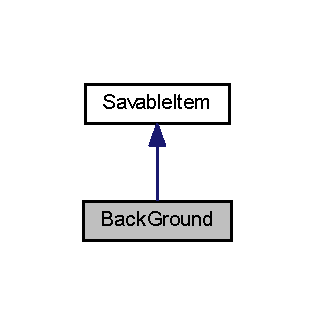
\includegraphics[width=151pt]{class_back_ground__inherit__graph}
\end{center}
\end{figure}


Граф связей класса Back\-Ground\-:
\nopagebreak
\begin{figure}[H]
\begin{center}
\leavevmode
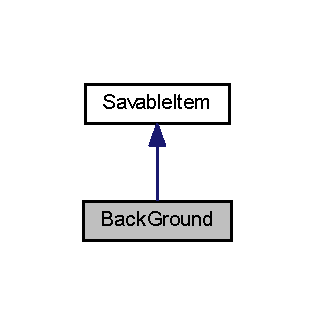
\includegraphics[width=151pt]{class_back_ground__coll__graph}
\end{center}
\end{figure}
\subsection*{Открытые члены}
\begin{DoxyCompactItemize}
\item 
\hyperlink{class_back_ground_a6a3fe7aa2ec8d57d372d336cd2d64337}{Back\-Ground} ()
\item 
virtual \hyperlink{class_back_ground_a6b14298ad37f17f054babadb2450f737}{$\sim$\-Back\-Ground} ()
\item 
void \hyperlink{class_back_ground_a3e779771d8962541787f3b9c1f265bd3}{Enable} (B\-O\-O\-L enable=T\-R\-U\-E)
\item 
void \hyperlink{class_back_ground_aa37dd21e916dcee3eee285103316b39e}{Get\-Colors} (C\-O\-L\-O\-R\-R\-E\-F \&\hyperlink{class_back_ground_ace5c696580cb70d04c43326e313d5086}{clr\-Start}, C\-O\-L\-O\-R\-R\-E\-F \&\hyperlink{class_back_ground_a76b44a73628e8503a1e56bc5253a5b1a}{clr\-Finish}) const 
\item 
void \hyperlink{class_back_ground_aa1000b4ae87a005caf92cbb10f948042}{Set\-Colors} (C\-O\-L\-O\-R\-R\-E\-F \hyperlink{class_back_ground_ace5c696580cb70d04c43326e313d5086}{clr\-Start}, C\-O\-L\-O\-R\-R\-E\-F \hyperlink{class_back_ground_a76b44a73628e8503a1e56bc5253a5b1a}{clr\-Finish})
\item 
void \hyperlink{class_back_ground_a65c9d4832f32f76967db4985b774f272}{Get\-Alpha\-Blend} (B\-Y\-T\-E \&\hyperlink{class_back_ground_ad3d27841bc53e26e464ed774aeaaad8d}{alpha\-Start}, B\-Y\-T\-E \&\hyperlink{class_back_ground_ae275790b73848c8919b63541ae948b0e}{alpha\-Finish}) const 
\item 
void \hyperlink{class_back_ground_a02d0cb2d464f0e90ca8cc430ffdc4553}{Set\-Alpha\-Blend} (B\-Y\-T\-E \hyperlink{class_back_ground_ad3d27841bc53e26e464ed774aeaaad8d}{alpha\-Start}, B\-Y\-T\-E \hyperlink{class_back_ground_ae275790b73848c8919b63541ae948b0e}{alpha\-Finish})
\item 
void \hyperlink{class_back_ground_a1e9833fea7630aa126314ede719a7776}{Set\-Gradient\-Direction} (B\-O\-O\-L \hyperlink{class_back_ground_a60e91e14cfea358477466c03bc918514}{vertical})
\item 
B\-O\-O\-L \hyperlink{class_back_ground_a1a10af7b8980d1268def9527f7e6cbce}{Get\-Gradient\-Direction} () const 
\item 
void \hyperlink{class_back_ground_a4e308cb320d9b028518c4fcdd3819ee6}{Set\-Rect} (const R\-E\-C\-T \&rc)
\item 
void \hyperlink{class_back_ground_afe1f339143f5c35bce336c130debf60e}{On\-Draw} (H\-D\-C hdc) const 
\item 
virtual B\-O\-O\-L \hyperlink{class_back_ground_ab21bb3686aac638ef0da5fb9a72c3925}{Write} (H\-A\-N\-D\-L\-E h\-File) const 
\item 
virtual B\-O\-O\-L \hyperlink{class_back_ground_aba05f03ff7484a1afad33c9400baf644}{Read} (H\-A\-N\-D\-L\-E h\-File)
\end{DoxyCompactItemize}
\subsection*{Открытые статические члены}
\begin{DoxyCompactItemize}
\item 
static void \hyperlink{class_back_ground_a3561380bde27c92d3f8457dcc3c7e91d}{Fill\-Rect\-With\-Gradient} (H\-D\-C hdc, const R\-E\-C\-T \&rc, C\-O\-L\-O\-R\-R\-E\-F clr1, C\-O\-L\-O\-R\-R\-E\-F clr2, B\-Y\-T\-E alpha1, B\-Y\-T\-E alpha2, B\-O\-O\-L b\-Vertical)
\end{DoxyCompactItemize}
\subsection*{Защищенные данные}
\begin{DoxyCompactItemize}
\item 
B\-O\-O\-L \hyperlink{class_back_ground_a7f8e544399813801ce7dc06509a4c062}{enabled}
\item 
C\-O\-L\-O\-R\-R\-E\-F \hyperlink{class_back_ground_ace5c696580cb70d04c43326e313d5086}{clr\-Start}
\item 
C\-O\-L\-O\-R\-R\-E\-F \hyperlink{class_back_ground_a76b44a73628e8503a1e56bc5253a5b1a}{clr\-Finish}
\item 
B\-Y\-T\-E \hyperlink{class_back_ground_ad3d27841bc53e26e464ed774aeaaad8d}{alpha\-Start}
\item 
B\-Y\-T\-E \hyperlink{class_back_ground_ae275790b73848c8919b63541ae948b0e}{alpha\-Finish}
\item 
B\-O\-O\-L \hyperlink{class_back_ground_a60e91e14cfea358477466c03bc918514}{vertical}
\item 
R\-E\-C\-T \hyperlink{class_back_ground_ab617902b70204abeba1512a5a85c3114}{rc\-Fill}
\end{DoxyCompactItemize}
\subsection*{Дополнительные унаследованные члены}


\subsection{Конструктор(ы)}
\hypertarget{class_back_ground_a6a3fe7aa2ec8d57d372d336cd2d64337}{\index{Back\-Ground@{Back\-Ground}!Back\-Ground@{Back\-Ground}}
\index{Back\-Ground@{Back\-Ground}!BackGround@{Back\-Ground}}
\subsubsection[{Back\-Ground}]{\setlength{\rightskip}{0pt plus 5cm}Back\-Ground\-::\-Back\-Ground (
\begin{DoxyParamCaption}
{}
\end{DoxyParamCaption}
)\hspace{0.3cm}{\ttfamily [inline]}}}\label{class_back_ground_a6a3fe7aa2ec8d57d372d336cd2d64337}
\hypertarget{class_back_ground_a6b14298ad37f17f054babadb2450f737}{\index{Back\-Ground@{Back\-Ground}!$\sim$\-Back\-Ground@{$\sim$\-Back\-Ground}}
\index{$\sim$\-Back\-Ground@{$\sim$\-Back\-Ground}!BackGround@{Back\-Ground}}
\subsubsection[{$\sim$\-Back\-Ground}]{\setlength{\rightskip}{0pt plus 5cm}virtual Back\-Ground\-::$\sim$\-Back\-Ground (
\begin{DoxyParamCaption}
{}
\end{DoxyParamCaption}
)\hspace{0.3cm}{\ttfamily [inline]}, {\ttfamily [virtual]}}}\label{class_back_ground_a6b14298ad37f17f054babadb2450f737}


\subsection{Методы}
\hypertarget{class_back_ground_a3e779771d8962541787f3b9c1f265bd3}{\index{Back\-Ground@{Back\-Ground}!Enable@{Enable}}
\index{Enable@{Enable}!BackGround@{Back\-Ground}}
\subsubsection[{Enable}]{\setlength{\rightskip}{0pt plus 5cm}void Back\-Ground\-::\-Enable (
\begin{DoxyParamCaption}
\item[{B\-O\-O\-L}]{enable = {\ttfamily TRUE}}
\end{DoxyParamCaption}
)\hspace{0.3cm}{\ttfamily [inline]}}}\label{class_back_ground_a3e779771d8962541787f3b9c1f265bd3}
\hypertarget{class_back_ground_a3561380bde27c92d3f8457dcc3c7e91d}{\index{Back\-Ground@{Back\-Ground}!Fill\-Rect\-With\-Gradient@{Fill\-Rect\-With\-Gradient}}
\index{Fill\-Rect\-With\-Gradient@{Fill\-Rect\-With\-Gradient}!BackGround@{Back\-Ground}}
\subsubsection[{Fill\-Rect\-With\-Gradient}]{\setlength{\rightskip}{0pt plus 5cm}void Back\-Ground\-::\-Fill\-Rect\-With\-Gradient (
\begin{DoxyParamCaption}
\item[{H\-D\-C}]{hdc, }
\item[{const R\-E\-C\-T \&}]{rc, }
\item[{C\-O\-L\-O\-R\-R\-E\-F}]{clr1, }
\item[{C\-O\-L\-O\-R\-R\-E\-F}]{clr2, }
\item[{B\-Y\-T\-E}]{alpha1, }
\item[{B\-Y\-T\-E}]{alpha2, }
\item[{B\-O\-O\-L}]{b\-Vertical}
\end{DoxyParamCaption}
)\hspace{0.3cm}{\ttfamily [static]}}}\label{class_back_ground_a3561380bde27c92d3f8457dcc3c7e91d}
\hypertarget{class_back_ground_a65c9d4832f32f76967db4985b774f272}{\index{Back\-Ground@{Back\-Ground}!Get\-Alpha\-Blend@{Get\-Alpha\-Blend}}
\index{Get\-Alpha\-Blend@{Get\-Alpha\-Blend}!BackGround@{Back\-Ground}}
\subsubsection[{Get\-Alpha\-Blend}]{\setlength{\rightskip}{0pt plus 5cm}void Back\-Ground\-::\-Get\-Alpha\-Blend (
\begin{DoxyParamCaption}
\item[{B\-Y\-T\-E \&}]{alpha\-Start, }
\item[{B\-Y\-T\-E \&}]{alpha\-Finish}
\end{DoxyParamCaption}
) const}}\label{class_back_ground_a65c9d4832f32f76967db4985b774f272}
\hypertarget{class_back_ground_aa37dd21e916dcee3eee285103316b39e}{\index{Back\-Ground@{Back\-Ground}!Get\-Colors@{Get\-Colors}}
\index{Get\-Colors@{Get\-Colors}!BackGround@{Back\-Ground}}
\subsubsection[{Get\-Colors}]{\setlength{\rightskip}{0pt plus 5cm}void Back\-Ground\-::\-Get\-Colors (
\begin{DoxyParamCaption}
\item[{C\-O\-L\-O\-R\-R\-E\-F \&}]{clr\-Start, }
\item[{C\-O\-L\-O\-R\-R\-E\-F \&}]{clr\-Finish}
\end{DoxyParamCaption}
) const}}\label{class_back_ground_aa37dd21e916dcee3eee285103316b39e}
\hypertarget{class_back_ground_a1a10af7b8980d1268def9527f7e6cbce}{\index{Back\-Ground@{Back\-Ground}!Get\-Gradient\-Direction@{Get\-Gradient\-Direction}}
\index{Get\-Gradient\-Direction@{Get\-Gradient\-Direction}!BackGround@{Back\-Ground}}
\subsubsection[{Get\-Gradient\-Direction}]{\setlength{\rightskip}{0pt plus 5cm}B\-O\-O\-L Back\-Ground\-::\-Get\-Gradient\-Direction (
\begin{DoxyParamCaption}
{}
\end{DoxyParamCaption}
) const\hspace{0.3cm}{\ttfamily [inline]}}}\label{class_back_ground_a1a10af7b8980d1268def9527f7e6cbce}
\hypertarget{class_back_ground_afe1f339143f5c35bce336c130debf60e}{\index{Back\-Ground@{Back\-Ground}!On\-Draw@{On\-Draw}}
\index{On\-Draw@{On\-Draw}!BackGround@{Back\-Ground}}
\subsubsection[{On\-Draw}]{\setlength{\rightskip}{0pt plus 5cm}void Back\-Ground\-::\-On\-Draw (
\begin{DoxyParamCaption}
\item[{H\-D\-C}]{hdc}
\end{DoxyParamCaption}
) const}}\label{class_back_ground_afe1f339143f5c35bce336c130debf60e}
\hypertarget{class_back_ground_aba05f03ff7484a1afad33c9400baf644}{\index{Back\-Ground@{Back\-Ground}!Read@{Read}}
\index{Read@{Read}!BackGround@{Back\-Ground}}
\subsubsection[{Read}]{\setlength{\rightskip}{0pt plus 5cm}B\-O\-O\-L Back\-Ground\-::\-Read (
\begin{DoxyParamCaption}
\item[{H\-A\-N\-D\-L\-E}]{h\-File}
\end{DoxyParamCaption}
)\hspace{0.3cm}{\ttfamily [virtual]}}}\label{class_back_ground_aba05f03ff7484a1afad33c9400baf644}


Замещает \hyperlink{class_savable_item_a7eadd16b2cb0652091cc15f596a00fb2}{Savable\-Item}.

\hypertarget{class_back_ground_a02d0cb2d464f0e90ca8cc430ffdc4553}{\index{Back\-Ground@{Back\-Ground}!Set\-Alpha\-Blend@{Set\-Alpha\-Blend}}
\index{Set\-Alpha\-Blend@{Set\-Alpha\-Blend}!BackGround@{Back\-Ground}}
\subsubsection[{Set\-Alpha\-Blend}]{\setlength{\rightskip}{0pt plus 5cm}void Back\-Ground\-::\-Set\-Alpha\-Blend (
\begin{DoxyParamCaption}
\item[{B\-Y\-T\-E}]{alpha\-Start, }
\item[{B\-Y\-T\-E}]{alpha\-Finish}
\end{DoxyParamCaption}
)}}\label{class_back_ground_a02d0cb2d464f0e90ca8cc430ffdc4553}
\hypertarget{class_back_ground_aa1000b4ae87a005caf92cbb10f948042}{\index{Back\-Ground@{Back\-Ground}!Set\-Colors@{Set\-Colors}}
\index{Set\-Colors@{Set\-Colors}!BackGround@{Back\-Ground}}
\subsubsection[{Set\-Colors}]{\setlength{\rightskip}{0pt plus 5cm}void Back\-Ground\-::\-Set\-Colors (
\begin{DoxyParamCaption}
\item[{C\-O\-L\-O\-R\-R\-E\-F}]{clr\-Start, }
\item[{C\-O\-L\-O\-R\-R\-E\-F}]{clr\-Finish}
\end{DoxyParamCaption}
)}}\label{class_back_ground_aa1000b4ae87a005caf92cbb10f948042}
\hypertarget{class_back_ground_a1e9833fea7630aa126314ede719a7776}{\index{Back\-Ground@{Back\-Ground}!Set\-Gradient\-Direction@{Set\-Gradient\-Direction}}
\index{Set\-Gradient\-Direction@{Set\-Gradient\-Direction}!BackGround@{Back\-Ground}}
\subsubsection[{Set\-Gradient\-Direction}]{\setlength{\rightskip}{0pt plus 5cm}void Back\-Ground\-::\-Set\-Gradient\-Direction (
\begin{DoxyParamCaption}
\item[{B\-O\-O\-L}]{vertical}
\end{DoxyParamCaption}
)\hspace{0.3cm}{\ttfamily [inline]}}}\label{class_back_ground_a1e9833fea7630aa126314ede719a7776}
\hypertarget{class_back_ground_a4e308cb320d9b028518c4fcdd3819ee6}{\index{Back\-Ground@{Back\-Ground}!Set\-Rect@{Set\-Rect}}
\index{Set\-Rect@{Set\-Rect}!BackGround@{Back\-Ground}}
\subsubsection[{Set\-Rect}]{\setlength{\rightskip}{0pt plus 5cm}void Back\-Ground\-::\-Set\-Rect (
\begin{DoxyParamCaption}
\item[{const R\-E\-C\-T \&}]{rc}
\end{DoxyParamCaption}
)}}\label{class_back_ground_a4e308cb320d9b028518c4fcdd3819ee6}
\hypertarget{class_back_ground_ab21bb3686aac638ef0da5fb9a72c3925}{\index{Back\-Ground@{Back\-Ground}!Write@{Write}}
\index{Write@{Write}!BackGround@{Back\-Ground}}
\subsubsection[{Write}]{\setlength{\rightskip}{0pt plus 5cm}B\-O\-O\-L Back\-Ground\-::\-Write (
\begin{DoxyParamCaption}
\item[{H\-A\-N\-D\-L\-E}]{h\-File}
\end{DoxyParamCaption}
) const\hspace{0.3cm}{\ttfamily [virtual]}}}\label{class_back_ground_ab21bb3686aac638ef0da5fb9a72c3925}


Замещает \hyperlink{class_savable_item_a0da511a4854f515096f8f9b498f64158}{Savable\-Item}.



\subsection{Данные класса}
\hypertarget{class_back_ground_ae275790b73848c8919b63541ae948b0e}{\index{Back\-Ground@{Back\-Ground}!alpha\-Finish@{alpha\-Finish}}
\index{alpha\-Finish@{alpha\-Finish}!BackGround@{Back\-Ground}}
\subsubsection[{alpha\-Finish}]{\setlength{\rightskip}{0pt plus 5cm}B\-Y\-T\-E Back\-Ground\-::alpha\-Finish\hspace{0.3cm}{\ttfamily [protected]}}}\label{class_back_ground_ae275790b73848c8919b63541ae948b0e}
\hypertarget{class_back_ground_ad3d27841bc53e26e464ed774aeaaad8d}{\index{Back\-Ground@{Back\-Ground}!alpha\-Start@{alpha\-Start}}
\index{alpha\-Start@{alpha\-Start}!BackGround@{Back\-Ground}}
\subsubsection[{alpha\-Start}]{\setlength{\rightskip}{0pt plus 5cm}B\-Y\-T\-E Back\-Ground\-::alpha\-Start\hspace{0.3cm}{\ttfamily [protected]}}}\label{class_back_ground_ad3d27841bc53e26e464ed774aeaaad8d}
\hypertarget{class_back_ground_a76b44a73628e8503a1e56bc5253a5b1a}{\index{Back\-Ground@{Back\-Ground}!clr\-Finish@{clr\-Finish}}
\index{clr\-Finish@{clr\-Finish}!BackGround@{Back\-Ground}}
\subsubsection[{clr\-Finish}]{\setlength{\rightskip}{0pt plus 5cm}C\-O\-L\-O\-R\-R\-E\-F Back\-Ground\-::clr\-Finish\hspace{0.3cm}{\ttfamily [protected]}}}\label{class_back_ground_a76b44a73628e8503a1e56bc5253a5b1a}
\hypertarget{class_back_ground_ace5c696580cb70d04c43326e313d5086}{\index{Back\-Ground@{Back\-Ground}!clr\-Start@{clr\-Start}}
\index{clr\-Start@{clr\-Start}!BackGround@{Back\-Ground}}
\subsubsection[{clr\-Start}]{\setlength{\rightskip}{0pt plus 5cm}C\-O\-L\-O\-R\-R\-E\-F Back\-Ground\-::clr\-Start\hspace{0.3cm}{\ttfamily [protected]}}}\label{class_back_ground_ace5c696580cb70d04c43326e313d5086}
\hypertarget{class_back_ground_a7f8e544399813801ce7dc06509a4c062}{\index{Back\-Ground@{Back\-Ground}!enabled@{enabled}}
\index{enabled@{enabled}!BackGround@{Back\-Ground}}
\subsubsection[{enabled}]{\setlength{\rightskip}{0pt plus 5cm}B\-O\-O\-L Back\-Ground\-::enabled\hspace{0.3cm}{\ttfamily [protected]}}}\label{class_back_ground_a7f8e544399813801ce7dc06509a4c062}
\hypertarget{class_back_ground_ab617902b70204abeba1512a5a85c3114}{\index{Back\-Ground@{Back\-Ground}!rc\-Fill@{rc\-Fill}}
\index{rc\-Fill@{rc\-Fill}!BackGround@{Back\-Ground}}
\subsubsection[{rc\-Fill}]{\setlength{\rightskip}{0pt plus 5cm}R\-E\-C\-T Back\-Ground\-::rc\-Fill\hspace{0.3cm}{\ttfamily [protected]}}}\label{class_back_ground_ab617902b70204abeba1512a5a85c3114}
\hypertarget{class_back_ground_a60e91e14cfea358477466c03bc918514}{\index{Back\-Ground@{Back\-Ground}!vertical@{vertical}}
\index{vertical@{vertical}!BackGround@{Back\-Ground}}
\subsubsection[{vertical}]{\setlength{\rightskip}{0pt plus 5cm}B\-O\-O\-L Back\-Ground\-::vertical\hspace{0.3cm}{\ttfamily [protected]}}}\label{class_back_ground_a60e91e14cfea358477466c03bc918514}


Объявления и описания членов классов находятся в файлах\-:\begin{DoxyCompactItemize}
\item 
src/\hyperlink{_back_ground_fill_8h}{Back\-Ground\-Fill.\-h}\item 
src/\hyperlink{_back_ground_fill_8cpp}{Back\-Ground\-Fill.\-cpp}\end{DoxyCompactItemize}

\hypertarget{class_base_message_exception}{\section{Класс Base\-Message\-Exception}
\label{class_base_message_exception}\index{Base\-Message\-Exception@{Base\-Message\-Exception}}
}


{\ttfamily \#include $<$exceptions.\-h$>$}



Граф наследования\-:Base\-Message\-Exception\-:
\nopagebreak
\begin{figure}[H]
\begin{center}
\leavevmode
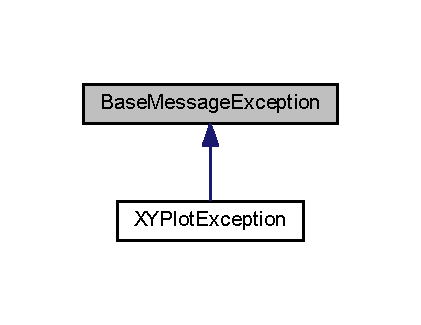
\includegraphics[width=202pt]{class_base_message_exception__inherit__graph}
\end{center}
\end{figure}
\subsection*{Открытые члены}
\begin{DoxyCompactItemize}
\item 
\hyperlink{class_base_message_exception_a61b9dad6f5b44ac8e3012e8b9af75ddf}{Base\-Message\-Exception} (std\-::string \hyperlink{class_base_message_exception_adbf18cd63b2f9a2bc6b0bbe20ce9da58}{message})
\item 
\hyperlink{class_base_message_exception_a2a9ae53ed316b0148db234f173d9d149}{$\sim$\-Base\-Message\-Exception} ()
\item 
const std\-::string \& \hyperlink{class_base_message_exception_ab9c5fefd3af3b24ac69877947ac6ace3}{Message} ()
\end{DoxyCompactItemize}
\subsection*{Защищенные данные}
\begin{DoxyCompactItemize}
\item 
std\-::string \hyperlink{class_base_message_exception_adbf18cd63b2f9a2bc6b0bbe20ce9da58}{message}
\end{DoxyCompactItemize}


\subsection{Конструктор(ы)}
\hypertarget{class_base_message_exception_a61b9dad6f5b44ac8e3012e8b9af75ddf}{\index{Base\-Message\-Exception@{Base\-Message\-Exception}!Base\-Message\-Exception@{Base\-Message\-Exception}}
\index{Base\-Message\-Exception@{Base\-Message\-Exception}!BaseMessageException@{Base\-Message\-Exception}}
\subsubsection[{Base\-Message\-Exception}]{\setlength{\rightskip}{0pt plus 5cm}Base\-Message\-Exception\-::\-Base\-Message\-Exception (
\begin{DoxyParamCaption}
\item[{std\-::string}]{message}
\end{DoxyParamCaption}
)\hspace{0.3cm}{\ttfamily [inline]}}}\label{class_base_message_exception_a61b9dad6f5b44ac8e3012e8b9af75ddf}
\hypertarget{class_base_message_exception_a2a9ae53ed316b0148db234f173d9d149}{\index{Base\-Message\-Exception@{Base\-Message\-Exception}!$\sim$\-Base\-Message\-Exception@{$\sim$\-Base\-Message\-Exception}}
\index{$\sim$\-Base\-Message\-Exception@{$\sim$\-Base\-Message\-Exception}!BaseMessageException@{Base\-Message\-Exception}}
\subsubsection[{$\sim$\-Base\-Message\-Exception}]{\setlength{\rightskip}{0pt plus 5cm}Base\-Message\-Exception\-::$\sim$\-Base\-Message\-Exception (
\begin{DoxyParamCaption}
{}
\end{DoxyParamCaption}
)\hspace{0.3cm}{\ttfamily [inline]}}}\label{class_base_message_exception_a2a9ae53ed316b0148db234f173d9d149}


\subsection{Методы}
\hypertarget{class_base_message_exception_ab9c5fefd3af3b24ac69877947ac6ace3}{\index{Base\-Message\-Exception@{Base\-Message\-Exception}!Message@{Message}}
\index{Message@{Message}!BaseMessageException@{Base\-Message\-Exception}}
\subsubsection[{Message}]{\setlength{\rightskip}{0pt plus 5cm}const std\-::string\& Base\-Message\-Exception\-::\-Message (
\begin{DoxyParamCaption}
{}
\end{DoxyParamCaption}
)\hspace{0.3cm}{\ttfamily [inline]}}}\label{class_base_message_exception_ab9c5fefd3af3b24ac69877947ac6ace3}


\subsection{Данные класса}
\hypertarget{class_base_message_exception_adbf18cd63b2f9a2bc6b0bbe20ce9da58}{\index{Base\-Message\-Exception@{Base\-Message\-Exception}!message@{message}}
\index{message@{message}!BaseMessageException@{Base\-Message\-Exception}}
\subsubsection[{message}]{\setlength{\rightskip}{0pt plus 5cm}std\-::string Base\-Message\-Exception\-::message\hspace{0.3cm}{\ttfamily [protected]}}}\label{class_base_message_exception_adbf18cd63b2f9a2bc6b0bbe20ce9da58}


Объявления и описания членов класса находятся в файле\-:\begin{DoxyCompactItemize}
\item 
src/\hyperlink{exceptions_8h}{exceptions.\-h}\end{DoxyCompactItemize}

\hypertarget{class_border}{\section{Класс Border}
\label{class_border}\index{Border@{Border}}
}


{\ttfamily \#include $<$border.\-h$>$}



Граф наследования\-:Border\-:
\nopagebreak
\begin{figure}[H]
\begin{center}
\leavevmode
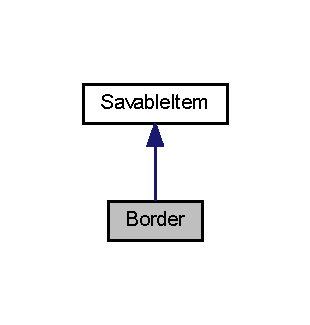
\includegraphics[width=149pt]{class_border__inherit__graph}
\end{center}
\end{figure}


Граф связей класса Border\-:
\nopagebreak
\begin{figure}[H]
\begin{center}
\leavevmode
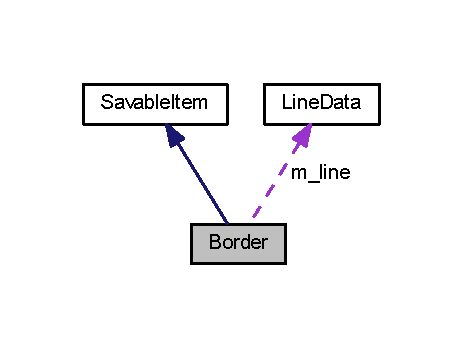
\includegraphics[width=222pt]{class_border__coll__graph}
\end{center}
\end{figure}
\subsection*{Открытые члены}
\begin{DoxyCompactItemize}
\item 
\hyperlink{class_border_a10716f049d192f79c42cd4fcf370645c}{Border} ()
\item 
virtual \hyperlink{class_border_a1987ed890f751ecb1dc9f5108b3354a4}{$\sim$\-Border} ()
\item 
\hyperlink{class_line_data}{Line\-Data} \& \hyperlink{class_border_a45871191f531c8fcb72de61be821ab12}{Get\-Line\-Data} ()
\item 
void \hyperlink{class_border_a0408de555f494a1e9b29a2687d708582}{Set\-Line\-Data} (const \hyperlink{class_line_data}{Line\-Data} \&line)
\item 
void \hyperlink{class_border_a4898438c8fd6c56d45754c2d86136f95}{Set\-Rect} (const R\-E\-C\-T \&self)
\item 
void \hyperlink{class_border_acf0e8ea07dbbb061c3f62c46c695e7a3}{Get\-Rect} (R\-E\-C\-T \&self) const 
\item 
void \hyperlink{class_border_a0b754dcefef27bb04f912480d8ba4537}{Enable} (B\-O\-O\-L enable)
\item 
B\-O\-O\-L \hyperlink{class_border_adf4ed3d2ef47f57a6f119fa0076679e0}{Is\-Enabled} () const 
\item 
void \hyperlink{class_border_a5747393117829b21310b78c23b95b7e5}{On\-Draw} (H\-D\-C hdc)
\item 
virtual B\-O\-O\-L \hyperlink{class_border_a61f82208fd693839acd08d0a4e787b10}{Write} (H\-A\-N\-D\-L\-E h\-File) const 
\item 
virtual B\-O\-O\-L \hyperlink{class_border_a35655b3874c3230038e171f18e7286f2}{Read} (H\-A\-N\-D\-L\-E h\-File)
\end{DoxyCompactItemize}
\subsection*{Защищенные данные}
\begin{DoxyCompactItemize}
\item 
int \hyperlink{class_border_a3c00eea5388d2f3bcd32d49c61200dfa}{m\-\_\-width}
\item 
B\-O\-O\-L \hyperlink{class_border_a63465529cd801a7697daa260e52cc156}{m\-\_\-enabled}
\item 
R\-E\-C\-T \hyperlink{class_border_a9abf5eb45c217515cde39e9ba877dd5d}{m\-\_\-self}
\item 
\hyperlink{class_line_data}{Line\-Data} \hyperlink{class_border_a77593373329183467369fb08d4818338}{m\-\_\-line}
\end{DoxyCompactItemize}
\subsection*{Дополнительные унаследованные члены}


\subsection{Конструктор(ы)}
\hypertarget{class_border_a10716f049d192f79c42cd4fcf370645c}{\index{Border@{Border}!Border@{Border}}
\index{Border@{Border}!Border@{Border}}
\subsubsection[{Border}]{\setlength{\rightskip}{0pt plus 5cm}Border\-::\-Border (
\begin{DoxyParamCaption}
{}
\end{DoxyParamCaption}
)}}\label{class_border_a10716f049d192f79c42cd4fcf370645c}
\hypertarget{class_border_a1987ed890f751ecb1dc9f5108b3354a4}{\index{Border@{Border}!$\sim$\-Border@{$\sim$\-Border}}
\index{$\sim$\-Border@{$\sim$\-Border}!Border@{Border}}
\subsubsection[{$\sim$\-Border}]{\setlength{\rightskip}{0pt plus 5cm}Border\-::$\sim$\-Border (
\begin{DoxyParamCaption}
{}
\end{DoxyParamCaption}
)\hspace{0.3cm}{\ttfamily [virtual]}}}\label{class_border_a1987ed890f751ecb1dc9f5108b3354a4}


\subsection{Методы}
\hypertarget{class_border_a0b754dcefef27bb04f912480d8ba4537}{\index{Border@{Border}!Enable@{Enable}}
\index{Enable@{Enable}!Border@{Border}}
\subsubsection[{Enable}]{\setlength{\rightskip}{0pt plus 5cm}void Border\-::\-Enable (
\begin{DoxyParamCaption}
\item[{B\-O\-O\-L}]{enable}
\end{DoxyParamCaption}
)\hspace{0.3cm}{\ttfamily [inline]}}}\label{class_border_a0b754dcefef27bb04f912480d8ba4537}
\hypertarget{class_border_a45871191f531c8fcb72de61be821ab12}{\index{Border@{Border}!Get\-Line\-Data@{Get\-Line\-Data}}
\index{Get\-Line\-Data@{Get\-Line\-Data}!Border@{Border}}
\subsubsection[{Get\-Line\-Data}]{\setlength{\rightskip}{0pt plus 5cm}{\bf Line\-Data}\& Border\-::\-Get\-Line\-Data (
\begin{DoxyParamCaption}
{}
\end{DoxyParamCaption}
)\hspace{0.3cm}{\ttfamily [inline]}}}\label{class_border_a45871191f531c8fcb72de61be821ab12}
\hypertarget{class_border_acf0e8ea07dbbb061c3f62c46c695e7a3}{\index{Border@{Border}!Get\-Rect@{Get\-Rect}}
\index{Get\-Rect@{Get\-Rect}!Border@{Border}}
\subsubsection[{Get\-Rect}]{\setlength{\rightskip}{0pt plus 5cm}void Border\-::\-Get\-Rect (
\begin{DoxyParamCaption}
\item[{R\-E\-C\-T \&}]{self}
\end{DoxyParamCaption}
) const\hspace{0.3cm}{\ttfamily [inline]}}}\label{class_border_acf0e8ea07dbbb061c3f62c46c695e7a3}
\hypertarget{class_border_adf4ed3d2ef47f57a6f119fa0076679e0}{\index{Border@{Border}!Is\-Enabled@{Is\-Enabled}}
\index{Is\-Enabled@{Is\-Enabled}!Border@{Border}}
\subsubsection[{Is\-Enabled}]{\setlength{\rightskip}{0pt plus 5cm}B\-O\-O\-L Border\-::\-Is\-Enabled (
\begin{DoxyParamCaption}
{}
\end{DoxyParamCaption}
) const\hspace{0.3cm}{\ttfamily [inline]}}}\label{class_border_adf4ed3d2ef47f57a6f119fa0076679e0}
\hypertarget{class_border_a5747393117829b21310b78c23b95b7e5}{\index{Border@{Border}!On\-Draw@{On\-Draw}}
\index{On\-Draw@{On\-Draw}!Border@{Border}}
\subsubsection[{On\-Draw}]{\setlength{\rightskip}{0pt plus 5cm}void Border\-::\-On\-Draw (
\begin{DoxyParamCaption}
\item[{H\-D\-C}]{hdc}
\end{DoxyParamCaption}
)}}\label{class_border_a5747393117829b21310b78c23b95b7e5}
\hypertarget{class_border_a35655b3874c3230038e171f18e7286f2}{\index{Border@{Border}!Read@{Read}}
\index{Read@{Read}!Border@{Border}}
\subsubsection[{Read}]{\setlength{\rightskip}{0pt plus 5cm}B\-O\-O\-L Border\-::\-Read (
\begin{DoxyParamCaption}
\item[{H\-A\-N\-D\-L\-E}]{h\-File}
\end{DoxyParamCaption}
)\hspace{0.3cm}{\ttfamily [virtual]}}}\label{class_border_a35655b3874c3230038e171f18e7286f2}


Замещает \hyperlink{class_savable_item_a7eadd16b2cb0652091cc15f596a00fb2}{Savable\-Item}.

\hypertarget{class_border_a0408de555f494a1e9b29a2687d708582}{\index{Border@{Border}!Set\-Line\-Data@{Set\-Line\-Data}}
\index{Set\-Line\-Data@{Set\-Line\-Data}!Border@{Border}}
\subsubsection[{Set\-Line\-Data}]{\setlength{\rightskip}{0pt plus 5cm}void Border\-::\-Set\-Line\-Data (
\begin{DoxyParamCaption}
\item[{const {\bf Line\-Data} \&}]{line}
\end{DoxyParamCaption}
)\hspace{0.3cm}{\ttfamily [inline]}}}\label{class_border_a0408de555f494a1e9b29a2687d708582}
\hypertarget{class_border_a4898438c8fd6c56d45754c2d86136f95}{\index{Border@{Border}!Set\-Rect@{Set\-Rect}}
\index{Set\-Rect@{Set\-Rect}!Border@{Border}}
\subsubsection[{Set\-Rect}]{\setlength{\rightskip}{0pt plus 5cm}void Border\-::\-Set\-Rect (
\begin{DoxyParamCaption}
\item[{const R\-E\-C\-T \&}]{self}
\end{DoxyParamCaption}
)\hspace{0.3cm}{\ttfamily [inline]}}}\label{class_border_a4898438c8fd6c56d45754c2d86136f95}
\hypertarget{class_border_a61f82208fd693839acd08d0a4e787b10}{\index{Border@{Border}!Write@{Write}}
\index{Write@{Write}!Border@{Border}}
\subsubsection[{Write}]{\setlength{\rightskip}{0pt plus 5cm}B\-O\-O\-L Border\-::\-Write (
\begin{DoxyParamCaption}
\item[{H\-A\-N\-D\-L\-E}]{h\-File}
\end{DoxyParamCaption}
) const\hspace{0.3cm}{\ttfamily [virtual]}}}\label{class_border_a61f82208fd693839acd08d0a4e787b10}


Замещает \hyperlink{class_savable_item_a0da511a4854f515096f8f9b498f64158}{Savable\-Item}.



\subsection{Данные класса}
\hypertarget{class_border_a63465529cd801a7697daa260e52cc156}{\index{Border@{Border}!m\-\_\-enabled@{m\-\_\-enabled}}
\index{m\-\_\-enabled@{m\-\_\-enabled}!Border@{Border}}
\subsubsection[{m\-\_\-enabled}]{\setlength{\rightskip}{0pt plus 5cm}B\-O\-O\-L Border\-::m\-\_\-enabled\hspace{0.3cm}{\ttfamily [protected]}}}\label{class_border_a63465529cd801a7697daa260e52cc156}
\hypertarget{class_border_a77593373329183467369fb08d4818338}{\index{Border@{Border}!m\-\_\-line@{m\-\_\-line}}
\index{m\-\_\-line@{m\-\_\-line}!Border@{Border}}
\subsubsection[{m\-\_\-line}]{\setlength{\rightskip}{0pt plus 5cm}{\bf Line\-Data} Border\-::m\-\_\-line\hspace{0.3cm}{\ttfamily [protected]}}}\label{class_border_a77593373329183467369fb08d4818338}
\hypertarget{class_border_a9abf5eb45c217515cde39e9ba877dd5d}{\index{Border@{Border}!m\-\_\-self@{m\-\_\-self}}
\index{m\-\_\-self@{m\-\_\-self}!Border@{Border}}
\subsubsection[{m\-\_\-self}]{\setlength{\rightskip}{0pt plus 5cm}R\-E\-C\-T Border\-::m\-\_\-self\hspace{0.3cm}{\ttfamily [protected]}}}\label{class_border_a9abf5eb45c217515cde39e9ba877dd5d}
\hypertarget{class_border_a3c00eea5388d2f3bcd32d49c61200dfa}{\index{Border@{Border}!m\-\_\-width@{m\-\_\-width}}
\index{m\-\_\-width@{m\-\_\-width}!Border@{Border}}
\subsubsection[{m\-\_\-width}]{\setlength{\rightskip}{0pt plus 5cm}int Border\-::m\-\_\-width\hspace{0.3cm}{\ttfamily [protected]}}}\label{class_border_a3c00eea5388d2f3bcd32d49c61200dfa}


Объявления и описания членов классов находятся в файлах\-:\begin{DoxyCompactItemize}
\item 
src/\hyperlink{border_8h}{border.\-h}\item 
src/\hyperlink{border_8cpp}{border.\-cpp}\end{DoxyCompactItemize}

\hypertarget{structdnp__checkout_1_1_c_a_l_l_g_a_t_e___d_e_s_c_r_i_p_t_o_r}{\section{Структура dnp\-\_\-checkout\-:\-:C\-A\-L\-L\-G\-A\-T\-E\-\_\-\-D\-E\-S\-C\-R\-I\-P\-T\-O\-R}
\label{structdnp__checkout_1_1_c_a_l_l_g_a_t_e___d_e_s_c_r_i_p_t_o_r}\index{dnp\-\_\-checkout\-::\-C\-A\-L\-L\-G\-A\-T\-E\-\_\-\-D\-E\-S\-C\-R\-I\-P\-T\-O\-R@{dnp\-\_\-checkout\-::\-C\-A\-L\-L\-G\-A\-T\-E\-\_\-\-D\-E\-S\-C\-R\-I\-P\-T\-O\-R}}
}
\subsection*{Открытые атрибуты}
\begin{DoxyCompactItemize}
\item 
W\-O\-R\-D \hyperlink{structdnp__checkout_1_1_c_a_l_l_g_a_t_e___d_e_s_c_r_i_p_t_o_r_a16553fe2bf118ead1e8c3010136a4304}{Offset\-\_\-0\-\_\-15}
\item 
W\-O\-R\-D \hyperlink{structdnp__checkout_1_1_c_a_l_l_g_a_t_e___d_e_s_c_r_i_p_t_o_r_ae619781e27c8a07bd1509b2df201be42}{Selector}
\item 
W\-O\-R\-D \hyperlink{structdnp__checkout_1_1_c_a_l_l_g_a_t_e___d_e_s_c_r_i_p_t_o_r_a3b8a86319111d57e27d03a3ff267ea8b}{Param\-Count}\-: 5
\item 
W\-O\-R\-D \hyperlink{structdnp__checkout_1_1_c_a_l_l_g_a_t_e___d_e_s_c_r_i_p_t_o_r_ac309a7299b11ca4d74956f2ed7b9cec1}{Unused}\-: 3
\item 
W\-O\-R\-D \hyperlink{structdnp__checkout_1_1_c_a_l_l_g_a_t_e___d_e_s_c_r_i_p_t_o_r_ab1864a24053c64c18ca11ff76590632a}{Type}\-: 4
\item 
W\-O\-R\-D \hyperlink{structdnp__checkout_1_1_c_a_l_l_g_a_t_e___d_e_s_c_r_i_p_t_o_r_af808fb075258cd4981fb61db9cbe7f73}{System}\-: 1
\item 
W\-O\-R\-D \hyperlink{structdnp__checkout_1_1_c_a_l_l_g_a_t_e___d_e_s_c_r_i_p_t_o_r_acb96a2a87acc898e4566a1eff83ca8f4}{D\-P\-L}\-: 2
\item 
W\-O\-R\-D \hyperlink{structdnp__checkout_1_1_c_a_l_l_g_a_t_e___d_e_s_c_r_i_p_t_o_r_aeb0fcded4f9eac8adacca728b963bf2f}{Present}\-: 1
\item 
W\-O\-R\-D \hyperlink{structdnp__checkout_1_1_c_a_l_l_g_a_t_e___d_e_s_c_r_i_p_t_o_r_a5ca902acc1370183732e7de86718cf5f}{Offset\-\_\-16\-\_\-31}
\end{DoxyCompactItemize}


\subsection{Данные класса}
\hypertarget{structdnp__checkout_1_1_c_a_l_l_g_a_t_e___d_e_s_c_r_i_p_t_o_r_acb96a2a87acc898e4566a1eff83ca8f4}{\index{dnp\-\_\-checkout\-::\-C\-A\-L\-L\-G\-A\-T\-E\-\_\-\-D\-E\-S\-C\-R\-I\-P\-T\-O\-R@{dnp\-\_\-checkout\-::\-C\-A\-L\-L\-G\-A\-T\-E\-\_\-\-D\-E\-S\-C\-R\-I\-P\-T\-O\-R}!D\-P\-L@{D\-P\-L}}
\index{D\-P\-L@{D\-P\-L}!dnp_checkout::CALLGATE_DESCRIPTOR@{dnp\-\_\-checkout\-::\-C\-A\-L\-L\-G\-A\-T\-E\-\_\-\-D\-E\-S\-C\-R\-I\-P\-T\-O\-R}}
\subsubsection[{D\-P\-L}]{\setlength{\rightskip}{0pt plus 5cm}W\-O\-R\-D dnp\-\_\-checkout\-::\-C\-A\-L\-L\-G\-A\-T\-E\-\_\-\-D\-E\-S\-C\-R\-I\-P\-T\-O\-R\-::\-D\-P\-L}}\label{structdnp__checkout_1_1_c_a_l_l_g_a_t_e___d_e_s_c_r_i_p_t_o_r_acb96a2a87acc898e4566a1eff83ca8f4}
\hypertarget{structdnp__checkout_1_1_c_a_l_l_g_a_t_e___d_e_s_c_r_i_p_t_o_r_a16553fe2bf118ead1e8c3010136a4304}{\index{dnp\-\_\-checkout\-::\-C\-A\-L\-L\-G\-A\-T\-E\-\_\-\-D\-E\-S\-C\-R\-I\-P\-T\-O\-R@{dnp\-\_\-checkout\-::\-C\-A\-L\-L\-G\-A\-T\-E\-\_\-\-D\-E\-S\-C\-R\-I\-P\-T\-O\-R}!Offset\-\_\-0\-\_\-15@{Offset\-\_\-0\-\_\-15}}
\index{Offset\-\_\-0\-\_\-15@{Offset\-\_\-0\-\_\-15}!dnp_checkout::CALLGATE_DESCRIPTOR@{dnp\-\_\-checkout\-::\-C\-A\-L\-L\-G\-A\-T\-E\-\_\-\-D\-E\-S\-C\-R\-I\-P\-T\-O\-R}}
\subsubsection[{Offset\-\_\-0\-\_\-15}]{\setlength{\rightskip}{0pt plus 5cm}W\-O\-R\-D dnp\-\_\-checkout\-::\-C\-A\-L\-L\-G\-A\-T\-E\-\_\-\-D\-E\-S\-C\-R\-I\-P\-T\-O\-R\-::\-Offset\-\_\-0\-\_\-15}}\label{structdnp__checkout_1_1_c_a_l_l_g_a_t_e___d_e_s_c_r_i_p_t_o_r_a16553fe2bf118ead1e8c3010136a4304}
\hypertarget{structdnp__checkout_1_1_c_a_l_l_g_a_t_e___d_e_s_c_r_i_p_t_o_r_a5ca902acc1370183732e7de86718cf5f}{\index{dnp\-\_\-checkout\-::\-C\-A\-L\-L\-G\-A\-T\-E\-\_\-\-D\-E\-S\-C\-R\-I\-P\-T\-O\-R@{dnp\-\_\-checkout\-::\-C\-A\-L\-L\-G\-A\-T\-E\-\_\-\-D\-E\-S\-C\-R\-I\-P\-T\-O\-R}!Offset\-\_\-16\-\_\-31@{Offset\-\_\-16\-\_\-31}}
\index{Offset\-\_\-16\-\_\-31@{Offset\-\_\-16\-\_\-31}!dnp_checkout::CALLGATE_DESCRIPTOR@{dnp\-\_\-checkout\-::\-C\-A\-L\-L\-G\-A\-T\-E\-\_\-\-D\-E\-S\-C\-R\-I\-P\-T\-O\-R}}
\subsubsection[{Offset\-\_\-16\-\_\-31}]{\setlength{\rightskip}{0pt plus 5cm}W\-O\-R\-D dnp\-\_\-checkout\-::\-C\-A\-L\-L\-G\-A\-T\-E\-\_\-\-D\-E\-S\-C\-R\-I\-P\-T\-O\-R\-::\-Offset\-\_\-16\-\_\-31}}\label{structdnp__checkout_1_1_c_a_l_l_g_a_t_e___d_e_s_c_r_i_p_t_o_r_a5ca902acc1370183732e7de86718cf5f}
\hypertarget{structdnp__checkout_1_1_c_a_l_l_g_a_t_e___d_e_s_c_r_i_p_t_o_r_a3b8a86319111d57e27d03a3ff267ea8b}{\index{dnp\-\_\-checkout\-::\-C\-A\-L\-L\-G\-A\-T\-E\-\_\-\-D\-E\-S\-C\-R\-I\-P\-T\-O\-R@{dnp\-\_\-checkout\-::\-C\-A\-L\-L\-G\-A\-T\-E\-\_\-\-D\-E\-S\-C\-R\-I\-P\-T\-O\-R}!Param\-Count@{Param\-Count}}
\index{Param\-Count@{Param\-Count}!dnp_checkout::CALLGATE_DESCRIPTOR@{dnp\-\_\-checkout\-::\-C\-A\-L\-L\-G\-A\-T\-E\-\_\-\-D\-E\-S\-C\-R\-I\-P\-T\-O\-R}}
\subsubsection[{Param\-Count}]{\setlength{\rightskip}{0pt plus 5cm}W\-O\-R\-D dnp\-\_\-checkout\-::\-C\-A\-L\-L\-G\-A\-T\-E\-\_\-\-D\-E\-S\-C\-R\-I\-P\-T\-O\-R\-::\-Param\-Count}}\label{structdnp__checkout_1_1_c_a_l_l_g_a_t_e___d_e_s_c_r_i_p_t_o_r_a3b8a86319111d57e27d03a3ff267ea8b}
\hypertarget{structdnp__checkout_1_1_c_a_l_l_g_a_t_e___d_e_s_c_r_i_p_t_o_r_aeb0fcded4f9eac8adacca728b963bf2f}{\index{dnp\-\_\-checkout\-::\-C\-A\-L\-L\-G\-A\-T\-E\-\_\-\-D\-E\-S\-C\-R\-I\-P\-T\-O\-R@{dnp\-\_\-checkout\-::\-C\-A\-L\-L\-G\-A\-T\-E\-\_\-\-D\-E\-S\-C\-R\-I\-P\-T\-O\-R}!Present@{Present}}
\index{Present@{Present}!dnp_checkout::CALLGATE_DESCRIPTOR@{dnp\-\_\-checkout\-::\-C\-A\-L\-L\-G\-A\-T\-E\-\_\-\-D\-E\-S\-C\-R\-I\-P\-T\-O\-R}}
\subsubsection[{Present}]{\setlength{\rightskip}{0pt plus 5cm}W\-O\-R\-D dnp\-\_\-checkout\-::\-C\-A\-L\-L\-G\-A\-T\-E\-\_\-\-D\-E\-S\-C\-R\-I\-P\-T\-O\-R\-::\-Present}}\label{structdnp__checkout_1_1_c_a_l_l_g_a_t_e___d_e_s_c_r_i_p_t_o_r_aeb0fcded4f9eac8adacca728b963bf2f}
\hypertarget{structdnp__checkout_1_1_c_a_l_l_g_a_t_e___d_e_s_c_r_i_p_t_o_r_ae619781e27c8a07bd1509b2df201be42}{\index{dnp\-\_\-checkout\-::\-C\-A\-L\-L\-G\-A\-T\-E\-\_\-\-D\-E\-S\-C\-R\-I\-P\-T\-O\-R@{dnp\-\_\-checkout\-::\-C\-A\-L\-L\-G\-A\-T\-E\-\_\-\-D\-E\-S\-C\-R\-I\-P\-T\-O\-R}!Selector@{Selector}}
\index{Selector@{Selector}!dnp_checkout::CALLGATE_DESCRIPTOR@{dnp\-\_\-checkout\-::\-C\-A\-L\-L\-G\-A\-T\-E\-\_\-\-D\-E\-S\-C\-R\-I\-P\-T\-O\-R}}
\subsubsection[{Selector}]{\setlength{\rightskip}{0pt plus 5cm}W\-O\-R\-D dnp\-\_\-checkout\-::\-C\-A\-L\-L\-G\-A\-T\-E\-\_\-\-D\-E\-S\-C\-R\-I\-P\-T\-O\-R\-::\-Selector}}\label{structdnp__checkout_1_1_c_a_l_l_g_a_t_e___d_e_s_c_r_i_p_t_o_r_ae619781e27c8a07bd1509b2df201be42}
\hypertarget{structdnp__checkout_1_1_c_a_l_l_g_a_t_e___d_e_s_c_r_i_p_t_o_r_af808fb075258cd4981fb61db9cbe7f73}{\index{dnp\-\_\-checkout\-::\-C\-A\-L\-L\-G\-A\-T\-E\-\_\-\-D\-E\-S\-C\-R\-I\-P\-T\-O\-R@{dnp\-\_\-checkout\-::\-C\-A\-L\-L\-G\-A\-T\-E\-\_\-\-D\-E\-S\-C\-R\-I\-P\-T\-O\-R}!System@{System}}
\index{System@{System}!dnp_checkout::CALLGATE_DESCRIPTOR@{dnp\-\_\-checkout\-::\-C\-A\-L\-L\-G\-A\-T\-E\-\_\-\-D\-E\-S\-C\-R\-I\-P\-T\-O\-R}}
\subsubsection[{System}]{\setlength{\rightskip}{0pt plus 5cm}W\-O\-R\-D dnp\-\_\-checkout\-::\-C\-A\-L\-L\-G\-A\-T\-E\-\_\-\-D\-E\-S\-C\-R\-I\-P\-T\-O\-R\-::\-System}}\label{structdnp__checkout_1_1_c_a_l_l_g_a_t_e___d_e_s_c_r_i_p_t_o_r_af808fb075258cd4981fb61db9cbe7f73}
\hypertarget{structdnp__checkout_1_1_c_a_l_l_g_a_t_e___d_e_s_c_r_i_p_t_o_r_ab1864a24053c64c18ca11ff76590632a}{\index{dnp\-\_\-checkout\-::\-C\-A\-L\-L\-G\-A\-T\-E\-\_\-\-D\-E\-S\-C\-R\-I\-P\-T\-O\-R@{dnp\-\_\-checkout\-::\-C\-A\-L\-L\-G\-A\-T\-E\-\_\-\-D\-E\-S\-C\-R\-I\-P\-T\-O\-R}!Type@{Type}}
\index{Type@{Type}!dnp_checkout::CALLGATE_DESCRIPTOR@{dnp\-\_\-checkout\-::\-C\-A\-L\-L\-G\-A\-T\-E\-\_\-\-D\-E\-S\-C\-R\-I\-P\-T\-O\-R}}
\subsubsection[{Type}]{\setlength{\rightskip}{0pt plus 5cm}W\-O\-R\-D dnp\-\_\-checkout\-::\-C\-A\-L\-L\-G\-A\-T\-E\-\_\-\-D\-E\-S\-C\-R\-I\-P\-T\-O\-R\-::\-Type}}\label{structdnp__checkout_1_1_c_a_l_l_g_a_t_e___d_e_s_c_r_i_p_t_o_r_ab1864a24053c64c18ca11ff76590632a}
\hypertarget{structdnp__checkout_1_1_c_a_l_l_g_a_t_e___d_e_s_c_r_i_p_t_o_r_ac309a7299b11ca4d74956f2ed7b9cec1}{\index{dnp\-\_\-checkout\-::\-C\-A\-L\-L\-G\-A\-T\-E\-\_\-\-D\-E\-S\-C\-R\-I\-P\-T\-O\-R@{dnp\-\_\-checkout\-::\-C\-A\-L\-L\-G\-A\-T\-E\-\_\-\-D\-E\-S\-C\-R\-I\-P\-T\-O\-R}!Unused@{Unused}}
\index{Unused@{Unused}!dnp_checkout::CALLGATE_DESCRIPTOR@{dnp\-\_\-checkout\-::\-C\-A\-L\-L\-G\-A\-T\-E\-\_\-\-D\-E\-S\-C\-R\-I\-P\-T\-O\-R}}
\subsubsection[{Unused}]{\setlength{\rightskip}{0pt plus 5cm}W\-O\-R\-D dnp\-\_\-checkout\-::\-C\-A\-L\-L\-G\-A\-T\-E\-\_\-\-D\-E\-S\-C\-R\-I\-P\-T\-O\-R\-::\-Unused}}\label{structdnp__checkout_1_1_c_a_l_l_g_a_t_e___d_e_s_c_r_i_p_t_o_r_ac309a7299b11ca4d74956f2ed7b9cec1}


Объявления и описания членов структуры находятся в файле\-:\begin{DoxyCompactItemize}
\item 
src/\hyperlink{dnp__checkout_8cpp}{dnp\-\_\-checkout.\-cpp}\end{DoxyCompactItemize}

\hypertarget{struct_c_a_l_l_g_a_t_e___d_e_s_c_r_i_p_t_o_r}{\section{Структура C\-A\-L\-L\-G\-A\-T\-E\-\_\-\-D\-E\-S\-C\-R\-I\-P\-T\-O\-R}
\label{struct_c_a_l_l_g_a_t_e___d_e_s_c_r_i_p_t_o_r}\index{C\-A\-L\-L\-G\-A\-T\-E\-\_\-\-D\-E\-S\-C\-R\-I\-P\-T\-O\-R@{C\-A\-L\-L\-G\-A\-T\-E\-\_\-\-D\-E\-S\-C\-R\-I\-P\-T\-O\-R}}
}


{\ttfamily \#include $<$port32.\-h$>$}

\subsection*{Открытые атрибуты}
\begin{DoxyCompactItemize}
\item 
W\-O\-R\-D \hyperlink{struct_c_a_l_l_g_a_t_e___d_e_s_c_r_i_p_t_o_r_a6f449fd6bf5a325a557c9ae4a5d90e26}{Offset\-\_\-0\-\_\-15}
\item 
W\-O\-R\-D \hyperlink{struct_c_a_l_l_g_a_t_e___d_e_s_c_r_i_p_t_o_r_ac7fd2d8e621350a3605d9eb96d156aca}{Selector}
\item 
W\-O\-R\-D \hyperlink{struct_c_a_l_l_g_a_t_e___d_e_s_c_r_i_p_t_o_r_a4c2fe3a00dbf9b9a501f12a870ff23c9}{Param\-Count}\-: 5
\item 
W\-O\-R\-D \hyperlink{struct_c_a_l_l_g_a_t_e___d_e_s_c_r_i_p_t_o_r_a438daced95d18f4cd40400fe329e9703}{Unused}\-: 3
\item 
W\-O\-R\-D \hyperlink{struct_c_a_l_l_g_a_t_e___d_e_s_c_r_i_p_t_o_r_afe8eeb6feb35759b5451fbaaff9b0492}{Type}\-: 4
\item 
W\-O\-R\-D \hyperlink{struct_c_a_l_l_g_a_t_e___d_e_s_c_r_i_p_t_o_r_a23159ce2d47f9d33d18e34382486a40a}{System}\-: 1
\item 
W\-O\-R\-D \hyperlink{struct_c_a_l_l_g_a_t_e___d_e_s_c_r_i_p_t_o_r_ab894af7ba4b99ca53fea9faf444b9616}{D\-P\-L}\-: 2
\item 
W\-O\-R\-D \hyperlink{struct_c_a_l_l_g_a_t_e___d_e_s_c_r_i_p_t_o_r_ad344e4cf67a98c0a408b4759bdec2b79}{Present}\-: 1
\item 
W\-O\-R\-D \hyperlink{struct_c_a_l_l_g_a_t_e___d_e_s_c_r_i_p_t_o_r_aea73ed7bc4012291b93523026753c346}{Offset\-\_\-16\-\_\-31}
\end{DoxyCompactItemize}


\subsection{Данные класса}
\hypertarget{struct_c_a_l_l_g_a_t_e___d_e_s_c_r_i_p_t_o_r_ab894af7ba4b99ca53fea9faf444b9616}{\index{C\-A\-L\-L\-G\-A\-T\-E\-\_\-\-D\-E\-S\-C\-R\-I\-P\-T\-O\-R@{C\-A\-L\-L\-G\-A\-T\-E\-\_\-\-D\-E\-S\-C\-R\-I\-P\-T\-O\-R}!D\-P\-L@{D\-P\-L}}
\index{D\-P\-L@{D\-P\-L}!CALLGATE_DESCRIPTOR@{C\-A\-L\-L\-G\-A\-T\-E\-\_\-\-D\-E\-S\-C\-R\-I\-P\-T\-O\-R}}
\subsubsection[{D\-P\-L}]{\setlength{\rightskip}{0pt plus 5cm}W\-O\-R\-D C\-A\-L\-L\-G\-A\-T\-E\-\_\-\-D\-E\-S\-C\-R\-I\-P\-T\-O\-R\-::\-D\-P\-L}}\label{struct_c_a_l_l_g_a_t_e___d_e_s_c_r_i_p_t_o_r_ab894af7ba4b99ca53fea9faf444b9616}
\hypertarget{struct_c_a_l_l_g_a_t_e___d_e_s_c_r_i_p_t_o_r_a6f449fd6bf5a325a557c9ae4a5d90e26}{\index{C\-A\-L\-L\-G\-A\-T\-E\-\_\-\-D\-E\-S\-C\-R\-I\-P\-T\-O\-R@{C\-A\-L\-L\-G\-A\-T\-E\-\_\-\-D\-E\-S\-C\-R\-I\-P\-T\-O\-R}!Offset\-\_\-0\-\_\-15@{Offset\-\_\-0\-\_\-15}}
\index{Offset\-\_\-0\-\_\-15@{Offset\-\_\-0\-\_\-15}!CALLGATE_DESCRIPTOR@{C\-A\-L\-L\-G\-A\-T\-E\-\_\-\-D\-E\-S\-C\-R\-I\-P\-T\-O\-R}}
\subsubsection[{Offset\-\_\-0\-\_\-15}]{\setlength{\rightskip}{0pt plus 5cm}W\-O\-R\-D C\-A\-L\-L\-G\-A\-T\-E\-\_\-\-D\-E\-S\-C\-R\-I\-P\-T\-O\-R\-::\-Offset\-\_\-0\-\_\-15}}\label{struct_c_a_l_l_g_a_t_e___d_e_s_c_r_i_p_t_o_r_a6f449fd6bf5a325a557c9ae4a5d90e26}
\hypertarget{struct_c_a_l_l_g_a_t_e___d_e_s_c_r_i_p_t_o_r_aea73ed7bc4012291b93523026753c346}{\index{C\-A\-L\-L\-G\-A\-T\-E\-\_\-\-D\-E\-S\-C\-R\-I\-P\-T\-O\-R@{C\-A\-L\-L\-G\-A\-T\-E\-\_\-\-D\-E\-S\-C\-R\-I\-P\-T\-O\-R}!Offset\-\_\-16\-\_\-31@{Offset\-\_\-16\-\_\-31}}
\index{Offset\-\_\-16\-\_\-31@{Offset\-\_\-16\-\_\-31}!CALLGATE_DESCRIPTOR@{C\-A\-L\-L\-G\-A\-T\-E\-\_\-\-D\-E\-S\-C\-R\-I\-P\-T\-O\-R}}
\subsubsection[{Offset\-\_\-16\-\_\-31}]{\setlength{\rightskip}{0pt plus 5cm}W\-O\-R\-D C\-A\-L\-L\-G\-A\-T\-E\-\_\-\-D\-E\-S\-C\-R\-I\-P\-T\-O\-R\-::\-Offset\-\_\-16\-\_\-31}}\label{struct_c_a_l_l_g_a_t_e___d_e_s_c_r_i_p_t_o_r_aea73ed7bc4012291b93523026753c346}
\hypertarget{struct_c_a_l_l_g_a_t_e___d_e_s_c_r_i_p_t_o_r_a4c2fe3a00dbf9b9a501f12a870ff23c9}{\index{C\-A\-L\-L\-G\-A\-T\-E\-\_\-\-D\-E\-S\-C\-R\-I\-P\-T\-O\-R@{C\-A\-L\-L\-G\-A\-T\-E\-\_\-\-D\-E\-S\-C\-R\-I\-P\-T\-O\-R}!Param\-Count@{Param\-Count}}
\index{Param\-Count@{Param\-Count}!CALLGATE_DESCRIPTOR@{C\-A\-L\-L\-G\-A\-T\-E\-\_\-\-D\-E\-S\-C\-R\-I\-P\-T\-O\-R}}
\subsubsection[{Param\-Count}]{\setlength{\rightskip}{0pt plus 5cm}W\-O\-R\-D C\-A\-L\-L\-G\-A\-T\-E\-\_\-\-D\-E\-S\-C\-R\-I\-P\-T\-O\-R\-::\-Param\-Count}}\label{struct_c_a_l_l_g_a_t_e___d_e_s_c_r_i_p_t_o_r_a4c2fe3a00dbf9b9a501f12a870ff23c9}
\hypertarget{struct_c_a_l_l_g_a_t_e___d_e_s_c_r_i_p_t_o_r_ad344e4cf67a98c0a408b4759bdec2b79}{\index{C\-A\-L\-L\-G\-A\-T\-E\-\_\-\-D\-E\-S\-C\-R\-I\-P\-T\-O\-R@{C\-A\-L\-L\-G\-A\-T\-E\-\_\-\-D\-E\-S\-C\-R\-I\-P\-T\-O\-R}!Present@{Present}}
\index{Present@{Present}!CALLGATE_DESCRIPTOR@{C\-A\-L\-L\-G\-A\-T\-E\-\_\-\-D\-E\-S\-C\-R\-I\-P\-T\-O\-R}}
\subsubsection[{Present}]{\setlength{\rightskip}{0pt plus 5cm}W\-O\-R\-D C\-A\-L\-L\-G\-A\-T\-E\-\_\-\-D\-E\-S\-C\-R\-I\-P\-T\-O\-R\-::\-Present}}\label{struct_c_a_l_l_g_a_t_e___d_e_s_c_r_i_p_t_o_r_ad344e4cf67a98c0a408b4759bdec2b79}
\hypertarget{struct_c_a_l_l_g_a_t_e___d_e_s_c_r_i_p_t_o_r_ac7fd2d8e621350a3605d9eb96d156aca}{\index{C\-A\-L\-L\-G\-A\-T\-E\-\_\-\-D\-E\-S\-C\-R\-I\-P\-T\-O\-R@{C\-A\-L\-L\-G\-A\-T\-E\-\_\-\-D\-E\-S\-C\-R\-I\-P\-T\-O\-R}!Selector@{Selector}}
\index{Selector@{Selector}!CALLGATE_DESCRIPTOR@{C\-A\-L\-L\-G\-A\-T\-E\-\_\-\-D\-E\-S\-C\-R\-I\-P\-T\-O\-R}}
\subsubsection[{Selector}]{\setlength{\rightskip}{0pt plus 5cm}W\-O\-R\-D C\-A\-L\-L\-G\-A\-T\-E\-\_\-\-D\-E\-S\-C\-R\-I\-P\-T\-O\-R\-::\-Selector}}\label{struct_c_a_l_l_g_a_t_e___d_e_s_c_r_i_p_t_o_r_ac7fd2d8e621350a3605d9eb96d156aca}
\hypertarget{struct_c_a_l_l_g_a_t_e___d_e_s_c_r_i_p_t_o_r_a23159ce2d47f9d33d18e34382486a40a}{\index{C\-A\-L\-L\-G\-A\-T\-E\-\_\-\-D\-E\-S\-C\-R\-I\-P\-T\-O\-R@{C\-A\-L\-L\-G\-A\-T\-E\-\_\-\-D\-E\-S\-C\-R\-I\-P\-T\-O\-R}!System@{System}}
\index{System@{System}!CALLGATE_DESCRIPTOR@{C\-A\-L\-L\-G\-A\-T\-E\-\_\-\-D\-E\-S\-C\-R\-I\-P\-T\-O\-R}}
\subsubsection[{System}]{\setlength{\rightskip}{0pt plus 5cm}W\-O\-R\-D C\-A\-L\-L\-G\-A\-T\-E\-\_\-\-D\-E\-S\-C\-R\-I\-P\-T\-O\-R\-::\-System}}\label{struct_c_a_l_l_g_a_t_e___d_e_s_c_r_i_p_t_o_r_a23159ce2d47f9d33d18e34382486a40a}
\hypertarget{struct_c_a_l_l_g_a_t_e___d_e_s_c_r_i_p_t_o_r_afe8eeb6feb35759b5451fbaaff9b0492}{\index{C\-A\-L\-L\-G\-A\-T\-E\-\_\-\-D\-E\-S\-C\-R\-I\-P\-T\-O\-R@{C\-A\-L\-L\-G\-A\-T\-E\-\_\-\-D\-E\-S\-C\-R\-I\-P\-T\-O\-R}!Type@{Type}}
\index{Type@{Type}!CALLGATE_DESCRIPTOR@{C\-A\-L\-L\-G\-A\-T\-E\-\_\-\-D\-E\-S\-C\-R\-I\-P\-T\-O\-R}}
\subsubsection[{Type}]{\setlength{\rightskip}{0pt plus 5cm}W\-O\-R\-D C\-A\-L\-L\-G\-A\-T\-E\-\_\-\-D\-E\-S\-C\-R\-I\-P\-T\-O\-R\-::\-Type}}\label{struct_c_a_l_l_g_a_t_e___d_e_s_c_r_i_p_t_o_r_afe8eeb6feb35759b5451fbaaff9b0492}
\hypertarget{struct_c_a_l_l_g_a_t_e___d_e_s_c_r_i_p_t_o_r_a438daced95d18f4cd40400fe329e9703}{\index{C\-A\-L\-L\-G\-A\-T\-E\-\_\-\-D\-E\-S\-C\-R\-I\-P\-T\-O\-R@{C\-A\-L\-L\-G\-A\-T\-E\-\_\-\-D\-E\-S\-C\-R\-I\-P\-T\-O\-R}!Unused@{Unused}}
\index{Unused@{Unused}!CALLGATE_DESCRIPTOR@{C\-A\-L\-L\-G\-A\-T\-E\-\_\-\-D\-E\-S\-C\-R\-I\-P\-T\-O\-R}}
\subsubsection[{Unused}]{\setlength{\rightskip}{0pt plus 5cm}W\-O\-R\-D C\-A\-L\-L\-G\-A\-T\-E\-\_\-\-D\-E\-S\-C\-R\-I\-P\-T\-O\-R\-::\-Unused}}\label{struct_c_a_l_l_g_a_t_e___d_e_s_c_r_i_p_t_o_r_a438daced95d18f4cd40400fe329e9703}


Объявления и описания членов структуры находятся в файле\-:\begin{DoxyCompactItemize}
\item 
src/\hyperlink{port32_8h}{port32.\-h}\end{DoxyCompactItemize}

\hypertarget{class_c_formatted_text_draw}{\section{Класс C\-Formatted\-Text\-Draw}
\label{class_c_formatted_text_draw}\index{C\-Formatted\-Text\-Draw@{C\-Formatted\-Text\-Draw}}
}


{\ttfamily \#include $<$formattedtextdraw.\-h$>$}



Граф наследования\-:C\-Formatted\-Text\-Draw\-:
\nopagebreak
\begin{figure}[H]
\begin{center}
\leavevmode
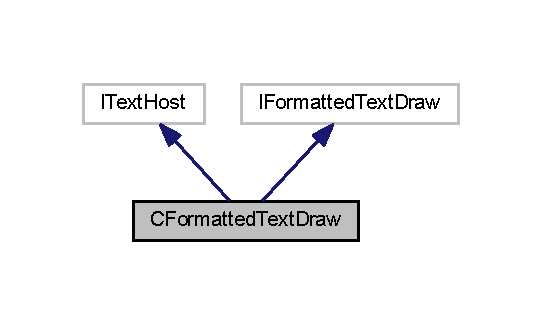
\includegraphics[width=260pt]{class_c_formatted_text_draw__inherit__graph}
\end{center}
\end{figure}


Граф связей класса C\-Formatted\-Text\-Draw\-:
\nopagebreak
\begin{figure}[H]
\begin{center}
\leavevmode
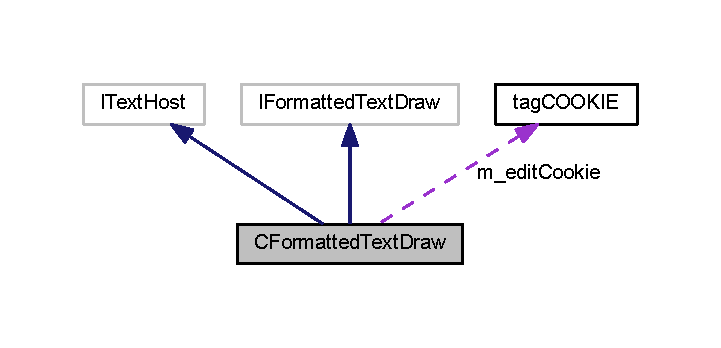
\includegraphics[width=346pt]{class_c_formatted_text_draw__coll__graph}
\end{center}
\end{figure}
\subsection*{Открытые члены}
\begin{DoxyCompactItemize}
\item 
\hyperlink{class_c_formatted_text_draw_aeedb5def68e1033d3759b142f48cfb8f}{C\-Formatted\-Text\-Draw} (H\-M\-O\-D\-U\-L\-E \hyperlink{class_c_formatted_text_draw_addc46f2c8df18b9be24193ac2b7bd261}{hmod})
\item 
\hyperlink{class_c_formatted_text_draw_a73cc74e417ded249eb7c8ba5026e74d6}{$\sim$\-C\-Formatted\-Text\-Draw} ()
\item 
H\-R\-E\-S\-U\-L\-T S\-T\-D\-M\-E\-T\-H\-O\-D\-C\-A\-L\-L\-T\-Y\-P\-E \hyperlink{class_c_formatted_text_draw_a94685a982152d40e47bbd38faf3d983d}{Query\-Interface} (R\-E\-F\-I\-I\-D riid, void \-\_\-\-\_\-\-R\-P\-C\-\_\-\-F\-A\-R $\ast$\-\_\-\-\_\-\-R\-P\-C\-\_\-\-F\-A\-R $\ast$ppv\-Object)
\item 
U\-L\-O\-N\-G S\-T\-D\-M\-E\-T\-H\-O\-D\-C\-A\-L\-L\-T\-Y\-P\-E \hyperlink{class_c_formatted_text_draw_adcdbb385f1b4e88c1bdd8f769cc2ea18}{Add\-Ref} (void)
\item 
U\-L\-O\-N\-G S\-T\-D\-M\-E\-T\-H\-O\-D\-C\-A\-L\-L\-T\-Y\-P\-E \hyperlink{class_c_formatted_text_draw_a8c0482c9982ab17a5b1bc16e42dae745}{Release} (void)
\item 
H\-R\-E\-S\-U\-L\-T \hyperlink{class_c_formatted_text_draw_a1b9dc72357c06a06f294d2e07bca4a18}{get\-\_\-\-Natural\-Height} (long Width, long $\ast$p\-Val)
\item 
H\-R\-E\-S\-U\-L\-T \hyperlink{class_c_formatted_text_draw_aa69166f66353dec9dc28b1e2e6f4c495}{get\-\_\-\-Natural\-Width} (long Height, long $\ast$p\-Val)
\item 
H\-R\-E\-S\-U\-L\-T \hyperlink{class_c_formatted_text_draw_aeda21fe76e87d85c6e6ae97f6d98c82c}{Create} ()
\item 
H\-R\-E\-S\-U\-L\-T \hyperlink{class_c_formatted_text_draw_aa9d8d11773fb62728bbee88d441edfcf}{Draw} (void $\ast$hdc\-Draw, R\-E\-C\-T $\ast$prc)
\item 
H\-R\-E\-S\-U\-L\-T \hyperlink{class_c_formatted_text_draw_ae319a9932c1a75ad19619bea99acb2df}{get\-\_\-\-R\-T\-F\-Text} (B\-S\-T\-R $\ast$p\-Val)
\item 
H\-R\-E\-S\-U\-L\-T \hyperlink{class_c_formatted_text_draw_aa8f8860ff9c0d5e1dacee5023743256f}{put\-\_\-\-R\-T\-F\-Text} (B\-S\-T\-R new\-Val)
\item 
H\-D\-C \hyperlink{class_c_formatted_text_draw_a82e2088a0416fc8a2d0039e97108ef6b}{Tx\-Get\-D\-C} ()
\item 
I\-N\-T \hyperlink{class_c_formatted_text_draw_a583a4401f0c1d5a3e5bf02c6a0cfedbd}{Tx\-Release\-D\-C} (H\-D\-C hdc)
\item 
B\-O\-O\-L \hyperlink{class_c_formatted_text_draw_a8b31bc8979880017bac423fc7861e3c4}{Tx\-Show\-Scroll\-Bar} (I\-N\-T fn\-Bar, B\-O\-O\-L f\-Show)
\item 
B\-O\-O\-L \hyperlink{class_c_formatted_text_draw_af376f10597fba86173093d88ef231c72}{Tx\-Enable\-Scroll\-Bar} (I\-N\-T fu\-S\-B\-Flags, I\-N\-T fu\-Arrowflags)
\item 
B\-O\-O\-L \hyperlink{class_c_formatted_text_draw_af1539757775ca0235713e93f42274553}{Tx\-Set\-Scroll\-Range} (I\-N\-T fn\-Bar, L\-O\-N\-G n\-Min\-Pos, I\-N\-T n\-Max\-Pos, B\-O\-O\-L f\-Redraw)
\item 
B\-O\-O\-L \hyperlink{class_c_formatted_text_draw_abfad442af7f3e31dc59b6abc23c789a4}{Tx\-Set\-Scroll\-Pos} (I\-N\-T fn\-Bar, I\-N\-T n\-Pos, B\-O\-O\-L f\-Redraw)
\item 
void \hyperlink{class_c_formatted_text_draw_afe30ef4cb3f37c9875ca64a3484e8af3}{Tx\-Invalidate\-Rect} (L\-P\-C\-R\-E\-C\-T prc, B\-O\-O\-L f\-Mode)
\item 
void \hyperlink{class_c_formatted_text_draw_abdb3f55080c4bc55d7710059beb9e6d4}{Tx\-View\-Change} (B\-O\-O\-L f\-Update)
\item 
B\-O\-O\-L \hyperlink{class_c_formatted_text_draw_a14b064dc9ea9d0e12fb49355756339df}{Tx\-Create\-Caret} (H\-B\-I\-T\-M\-A\-P hbmp, I\-N\-T x\-Width, I\-N\-T y\-Height)
\item 
B\-O\-O\-L \hyperlink{class_c_formatted_text_draw_ab2559df2077f47c4483ba526727016e2}{Tx\-Show\-Caret} (B\-O\-O\-L f\-Show)
\item 
B\-O\-O\-L \hyperlink{class_c_formatted_text_draw_a0de9d25f5f37cb97c45323f8ebaff5a1}{Tx\-Set\-Caret\-Pos} (I\-N\-T x, I\-N\-T y)
\item 
B\-O\-O\-L \hyperlink{class_c_formatted_text_draw_a2cfee5142c0ccc914ab9e22be37021a1}{Tx\-Set\-Timer} (U\-I\-N\-T id\-Timer, U\-I\-N\-T u\-Timeout)
\item 
void \hyperlink{class_c_formatted_text_draw_acea0cb499a41c7a3b8471ccae713d0a2}{Tx\-Kill\-Timer} (U\-I\-N\-T id\-Timer)
\item 
void \hyperlink{class_c_formatted_text_draw_ab86cfe0bd348ba7e6dca937139bf594b}{Tx\-Scroll\-Window\-Ex} (I\-N\-T dx, I\-N\-T dy, L\-P\-C\-R\-E\-C\-T lprc\-Scroll, L\-P\-C\-R\-E\-C\-T lprc\-Clip, H\-R\-G\-N hrgn\-Update, L\-P\-R\-E\-C\-T lprc\-Update, U\-I\-N\-T fu\-Scroll)
\item 
void \hyperlink{class_c_formatted_text_draw_a44ef4a7a47a5be7d277d4b04e7e12a27}{Tx\-Set\-Capture} (B\-O\-O\-L f\-Capture)
\item 
void \hyperlink{class_c_formatted_text_draw_ae1f80562f0bb57e63f88ca07184a7290}{Tx\-Set\-Focus} ()
\item 
void \hyperlink{class_c_formatted_text_draw_ab1f8c8017864381e356371f36d7e6863}{Tx\-Set\-Cursor} (H\-C\-U\-R\-S\-O\-R hcur, B\-O\-O\-L f\-Text)
\item 
B\-O\-O\-L \hyperlink{class_c_formatted_text_draw_a5bbd1e639e6c48c33a6bfaa0d469e439}{Tx\-Screen\-To\-Client} (L\-P\-P\-O\-I\-N\-T lppt)
\item 
B\-O\-O\-L \hyperlink{class_c_formatted_text_draw_abb05d3c20125bb481a5256272d87b67f}{Tx\-Client\-To\-Screen} (L\-P\-P\-O\-I\-N\-T lppt)
\item 
H\-R\-E\-S\-U\-L\-T \hyperlink{class_c_formatted_text_draw_a94abf3aa085118853e6fb343dc56dbd1}{Tx\-Activate} (L\-O\-N\-G $\ast$pl\-Old\-State)
\item 
H\-R\-E\-S\-U\-L\-T \hyperlink{class_c_formatted_text_draw_a4f578fb1c8066bffccbe08661a58b3a9}{Tx\-Deactivate} (L\-O\-N\-G l\-New\-State)
\item 
H\-R\-E\-S\-U\-L\-T \hyperlink{class_c_formatted_text_draw_a7d26debc0162611ce308b7472e816a0e}{Tx\-Get\-Client\-Rect} (L\-P\-R\-E\-C\-T prc)
\item 
H\-R\-E\-S\-U\-L\-T \hyperlink{class_c_formatted_text_draw_a356e5054a4a70bfddebfa5456a51c0f2}{Tx\-Get\-View\-Inset} (L\-P\-R\-E\-C\-T prc)
\item 
H\-R\-E\-S\-U\-L\-T \hyperlink{class_c_formatted_text_draw_a1b6bf84a20ce406266dcd59e05579faa}{Tx\-Get\-Char\-Format} (const C\-H\-A\-R\-F\-O\-R\-M\-A\-T\-W $\ast$$\ast$pp\-C\-F)
\item 
H\-R\-E\-S\-U\-L\-T \hyperlink{class_c_formatted_text_draw_a9fcc615f0abc3edd55a5bc6eb07245c0}{Tx\-Get\-Para\-Format} (const P\-A\-R\-A\-F\-O\-R\-M\-A\-T $\ast$$\ast$pp\-P\-F)
\item 
C\-O\-L\-O\-R\-R\-E\-F \hyperlink{class_c_formatted_text_draw_a87bf95137cb9c82cf3b5b184d7b499cd}{Tx\-Get\-Sys\-Color} (int n\-Index)
\item 
H\-R\-E\-S\-U\-L\-T \hyperlink{class_c_formatted_text_draw_aae9e30620f85cd0855da77eefab5c542}{Tx\-Get\-Back\-Style} (T\-X\-T\-B\-A\-C\-K\-S\-T\-Y\-L\-E $\ast$pstyle)
\item 
H\-R\-E\-S\-U\-L\-T \hyperlink{class_c_formatted_text_draw_ac16e3287c2da3f1d4af57d268339b3b0}{Tx\-Get\-Max\-Length} (D\-W\-O\-R\-D $\ast$plength)
\item 
H\-R\-E\-S\-U\-L\-T \hyperlink{class_c_formatted_text_draw_a0d11953e055809df98a3354a7b48eff7}{Tx\-Get\-Scroll\-Bars} (D\-W\-O\-R\-D $\ast$pdw\-Scroll\-Bar)
\item 
H\-R\-E\-S\-U\-L\-T \hyperlink{class_c_formatted_text_draw_ac64a3d02efa70493ee449dace1fea36c}{Tx\-Get\-Password\-Char} (T\-C\-H\-A\-R $\ast$pch)
\item 
H\-R\-E\-S\-U\-L\-T \hyperlink{class_c_formatted_text_draw_a45973a797c196a9d7cf02127d12e7a54}{Tx\-Get\-Accelerator\-Pos} (L\-O\-N\-G $\ast$pcp)
\item 
H\-R\-E\-S\-U\-L\-T \hyperlink{class_c_formatted_text_draw_a9247dfc9e0cce9f1942c5b6c632ed78d}{Tx\-Get\-Extent} (L\-P\-S\-I\-Z\-E\-L lp\-Extent)
\item 
H\-R\-E\-S\-U\-L\-T \hyperlink{class_c_formatted_text_draw_aa12d7dee46f52f789b6b2109008948c3}{On\-Tx\-Char\-Format\-Change} (const C\-H\-A\-R\-F\-O\-R\-M\-A\-T\-W $\ast$pcf)
\item 
H\-R\-E\-S\-U\-L\-T \hyperlink{class_c_formatted_text_draw_a01a2da9e321236594b6f3fe8bb0ac310}{On\-Tx\-Para\-Format\-Change} (const P\-A\-R\-A\-F\-O\-R\-M\-A\-T $\ast$ppf)
\item 
H\-R\-E\-S\-U\-L\-T \hyperlink{class_c_formatted_text_draw_a43579a9dbb4bd8031cdf7dd1c5a2d008}{Tx\-Get\-Property\-Bits} (D\-W\-O\-R\-D dw\-Mask, D\-W\-O\-R\-D $\ast$pdw\-Bits)
\item 
H\-R\-E\-S\-U\-L\-T \hyperlink{class_c_formatted_text_draw_a7d7aa1164fef848f8cc86084ff0d5947}{Tx\-Notify} (D\-W\-O\-R\-D i\-Notify, void $\ast$pv)
\item 
H\-I\-M\-C \hyperlink{class_c_formatted_text_draw_aeca2dd3918ef62d7f7c030f1a2add1dd}{Tx\-Imm\-Get\-Context} ()
\item 
void \hyperlink{class_c_formatted_text_draw_a677a0528e12025ac1d834ebb3fe17f4f}{Tx\-Imm\-Release\-Context} (H\-I\-M\-C himc)
\item 
H\-R\-E\-S\-U\-L\-T \hyperlink{class_c_formatted_text_draw_a26d3e8e94e5ec00f2670737ad565bb50}{Tx\-Get\-Selection\-Bar\-Width} (L\-O\-N\-G $\ast$l\-Sel\-Bar\-Width)
\item 
H\-R\-E\-S\-U\-L\-T \hyperlink{class_c_formatted_text_draw_a9ce824728f92e00b317b59d8b935d86e}{Set\-Text\-Color} (C\-O\-L\-O\-R\-R\-E\-F clr)
\item 
H\-R\-E\-S\-U\-L\-T \hyperlink{class_c_formatted_text_draw_ac3ff1149d0e0ac7da420bc71d1fc2be1}{Set\-Text\-Font} (H\-F\-O\-N\-T font)
\item 
H\-R\-E\-S\-U\-L\-T \hyperlink{class_c_formatted_text_draw_a55723aacd9eea72087f4a8c1716c44e8}{Char\-Format\-From\-H\-F\-O\-N\-T} (C\-H\-A\-R\-F\-O\-R\-M\-A\-T2\-W $\ast$p\-C\-F, H\-F\-O\-N\-T h\-Font)
\item 
H\-R\-E\-S\-U\-L\-T \hyperlink{class_c_formatted_text_draw_a84688cc43aa013fc01eab25bcf687809}{Init\-Default\-Char\-Format} ()
\item 
H\-R\-E\-S\-U\-L\-T \hyperlink{class_c_formatted_text_draw_adf8e13c8ba939b994d4235b588a52177}{Init\-Default\-Para\-Format} ()
\item 
H\-R\-E\-S\-U\-L\-T \hyperlink{class_c_formatted_text_draw_aacdbc394944e8ca679c5de2e824496d5}{Create\-Text\-Services\-Object} ()
\end{DoxyCompactItemize}
\subsection*{Открытые атрибуты}
\begin{DoxyCompactItemize}
\item 
R\-E\-C\-T \hyperlink{class_c_formatted_text_draw_ac12889a14954434340548415c24cd61c}{m\-\_\-rc\-Client}
\item 
R\-E\-C\-T \hyperlink{class_c_formatted_text_draw_a55dfce4f5f6ceebc265f50d39a3e3b18}{m\-\_\-rc\-View\-Inset}
\item 
S\-I\-Z\-E\-L \hyperlink{class_c_formatted_text_draw_a7a01811c4c6123bea7d639302b69a128}{m\-\_\-sizel\-Extent}
\item 
int \hyperlink{class_c_formatted_text_draw_af07e4ff84b148e4c1614782ec37b9b54}{n\-Pixels\-Per\-Inch\-X}
\item 
int \hyperlink{class_c_formatted_text_draw_aed39a1517760cfb53599780e231d481b}{n\-Pixels\-Per\-Inch\-Y}
\item 
C\-H\-A\-R\-F\-O\-R\-M\-A\-T2\-W $\ast$ \hyperlink{class_c_formatted_text_draw_add7687bda35106a487299a6bd945e0fe}{m\-\_\-p\-C\-F}
\item 
P\-A\-R\-A\-F\-O\-R\-M\-A\-T2 \hyperlink{class_c_formatted_text_draw_ae5c1b692255587fff873eb3cae1e30a0}{m\-\_\-\-P\-F}
\item 
D\-W\-O\-R\-D \hyperlink{class_c_formatted_text_draw_ae015d2a67f789b83b172077ca92fedba}{m\-\_\-dw\-Scrollbar}
\item 
D\-W\-O\-R\-D \hyperlink{class_c_formatted_text_draw_a4877370e9f9a97ca802f614601ca972c}{m\-\_\-dw\-Property\-Bits}
\item 
D\-W\-O\-R\-D \hyperlink{class_c_formatted_text_draw_a95e778f91604bec6f68d7933550910aa}{m\-\_\-dw\-Max\-Length}
\item 
\hyperlink{formattedtextdraw_8h_a38853a4ceee8d1a6fac128d822488cdc}{C\-O\-O\-K\-I\-E} \hyperlink{class_c_formatted_text_draw_ac3b581340c521c7f372bcce0792e3059}{m\-\_\-edit\-Cookie}
\item 
I\-Text\-Services $\ast$ \hyperlink{class_c_formatted_text_draw_a359702fb97b39932d0f4605f2324c1d3}{m\-\_\-sp\-Text\-Services}
\item 
B\-S\-T\-R \hyperlink{class_c_formatted_text_draw_ae25f82f2e2222357070087b218fcc849}{m\-\_\-\-R\-T\-F\-Text}
\item 
H\-M\-O\-D\-U\-L\-E \hyperlink{class_c_formatted_text_draw_addc46f2c8df18b9be24193ac2b7bd261}{hmod}
\end{DoxyCompactItemize}


\subsection{Конструктор(ы)}
\hypertarget{class_c_formatted_text_draw_aeedb5def68e1033d3759b142f48cfb8f}{\index{C\-Formatted\-Text\-Draw@{C\-Formatted\-Text\-Draw}!C\-Formatted\-Text\-Draw@{C\-Formatted\-Text\-Draw}}
\index{C\-Formatted\-Text\-Draw@{C\-Formatted\-Text\-Draw}!CFormattedTextDraw@{C\-Formatted\-Text\-Draw}}
\subsubsection[{C\-Formatted\-Text\-Draw}]{\setlength{\rightskip}{0pt plus 5cm}C\-Formatted\-Text\-Draw\-::\-C\-Formatted\-Text\-Draw (
\begin{DoxyParamCaption}
\item[{H\-M\-O\-D\-U\-L\-E}]{hmod}
\end{DoxyParamCaption}
)\hspace{0.3cm}{\ttfamily [inline]}}}\label{class_c_formatted_text_draw_aeedb5def68e1033d3759b142f48cfb8f}
\hypertarget{class_c_formatted_text_draw_a73cc74e417ded249eb7c8ba5026e74d6}{\index{C\-Formatted\-Text\-Draw@{C\-Formatted\-Text\-Draw}!$\sim$\-C\-Formatted\-Text\-Draw@{$\sim$\-C\-Formatted\-Text\-Draw}}
\index{$\sim$\-C\-Formatted\-Text\-Draw@{$\sim$\-C\-Formatted\-Text\-Draw}!CFormattedTextDraw@{C\-Formatted\-Text\-Draw}}
\subsubsection[{$\sim$\-C\-Formatted\-Text\-Draw}]{\setlength{\rightskip}{0pt plus 5cm}C\-Formatted\-Text\-Draw\-::$\sim$\-C\-Formatted\-Text\-Draw (
\begin{DoxyParamCaption}
{}
\end{DoxyParamCaption}
)}}\label{class_c_formatted_text_draw_a73cc74e417ded249eb7c8ba5026e74d6}


\subsection{Методы}
\hypertarget{class_c_formatted_text_draw_adcdbb385f1b4e88c1bdd8f769cc2ea18}{\index{C\-Formatted\-Text\-Draw@{C\-Formatted\-Text\-Draw}!Add\-Ref@{Add\-Ref}}
\index{Add\-Ref@{Add\-Ref}!CFormattedTextDraw@{C\-Formatted\-Text\-Draw}}
\subsubsection[{Add\-Ref}]{\setlength{\rightskip}{0pt plus 5cm}U\-L\-O\-N\-G S\-T\-D\-M\-E\-T\-H\-O\-D\-C\-A\-L\-L\-T\-Y\-P\-E C\-Formatted\-Text\-Draw\-::\-Add\-Ref (
\begin{DoxyParamCaption}
\item[{void}]{}
\end{DoxyParamCaption}
)\hspace{0.3cm}{\ttfamily [inline]}}}\label{class_c_formatted_text_draw_adcdbb385f1b4e88c1bdd8f769cc2ea18}
\hypertarget{class_c_formatted_text_draw_a55723aacd9eea72087f4a8c1716c44e8}{\index{C\-Formatted\-Text\-Draw@{C\-Formatted\-Text\-Draw}!Char\-Format\-From\-H\-F\-O\-N\-T@{Char\-Format\-From\-H\-F\-O\-N\-T}}
\index{Char\-Format\-From\-H\-F\-O\-N\-T@{Char\-Format\-From\-H\-F\-O\-N\-T}!CFormattedTextDraw@{C\-Formatted\-Text\-Draw}}
\subsubsection[{Char\-Format\-From\-H\-F\-O\-N\-T}]{\setlength{\rightskip}{0pt plus 5cm}H\-R\-E\-S\-U\-L\-T C\-Formatted\-Text\-Draw\-::\-Char\-Format\-From\-H\-F\-O\-N\-T (
\begin{DoxyParamCaption}
\item[{C\-H\-A\-R\-F\-O\-R\-M\-A\-T2\-W $\ast$}]{p\-C\-F, }
\item[{H\-F\-O\-N\-T}]{h\-Font}
\end{DoxyParamCaption}
)}}\label{class_c_formatted_text_draw_a55723aacd9eea72087f4a8c1716c44e8}
\hypertarget{class_c_formatted_text_draw_aeda21fe76e87d85c6e6ae97f6d98c82c}{\index{C\-Formatted\-Text\-Draw@{C\-Formatted\-Text\-Draw}!Create@{Create}}
\index{Create@{Create}!CFormattedTextDraw@{C\-Formatted\-Text\-Draw}}
\subsubsection[{Create}]{\setlength{\rightskip}{0pt plus 5cm}H\-R\-E\-S\-U\-L\-T C\-Formatted\-Text\-Draw\-::\-Create (
\begin{DoxyParamCaption}
{}
\end{DoxyParamCaption}
)}}\label{class_c_formatted_text_draw_aeda21fe76e87d85c6e6ae97f6d98c82c}
\hypertarget{class_c_formatted_text_draw_aacdbc394944e8ca679c5de2e824496d5}{\index{C\-Formatted\-Text\-Draw@{C\-Formatted\-Text\-Draw}!Create\-Text\-Services\-Object@{Create\-Text\-Services\-Object}}
\index{Create\-Text\-Services\-Object@{Create\-Text\-Services\-Object}!CFormattedTextDraw@{C\-Formatted\-Text\-Draw}}
\subsubsection[{Create\-Text\-Services\-Object}]{\setlength{\rightskip}{0pt plus 5cm}H\-R\-E\-S\-U\-L\-T C\-Formatted\-Text\-Draw\-::\-Create\-Text\-Services\-Object (
\begin{DoxyParamCaption}
{}
\end{DoxyParamCaption}
)}}\label{class_c_formatted_text_draw_aacdbc394944e8ca679c5de2e824496d5}
\hypertarget{class_c_formatted_text_draw_aa9d8d11773fb62728bbee88d441edfcf}{\index{C\-Formatted\-Text\-Draw@{C\-Formatted\-Text\-Draw}!Draw@{Draw}}
\index{Draw@{Draw}!CFormattedTextDraw@{C\-Formatted\-Text\-Draw}}
\subsubsection[{Draw}]{\setlength{\rightskip}{0pt plus 5cm}H\-R\-E\-S\-U\-L\-T C\-Formatted\-Text\-Draw\-::\-Draw (
\begin{DoxyParamCaption}
\item[{void $\ast$}]{hdc\-Draw, }
\item[{R\-E\-C\-T $\ast$}]{prc}
\end{DoxyParamCaption}
)}}\label{class_c_formatted_text_draw_aa9d8d11773fb62728bbee88d441edfcf}
\hypertarget{class_c_formatted_text_draw_a1b9dc72357c06a06f294d2e07bca4a18}{\index{C\-Formatted\-Text\-Draw@{C\-Formatted\-Text\-Draw}!get\-\_\-\-Natural\-Height@{get\-\_\-\-Natural\-Height}}
\index{get\-\_\-\-Natural\-Height@{get\-\_\-\-Natural\-Height}!CFormattedTextDraw@{C\-Formatted\-Text\-Draw}}
\subsubsection[{get\-\_\-\-Natural\-Height}]{\setlength{\rightskip}{0pt plus 5cm}H\-R\-E\-S\-U\-L\-T C\-Formatted\-Text\-Draw\-::get\-\_\-\-Natural\-Height (
\begin{DoxyParamCaption}
\item[{long}]{Width, }
\item[{long $\ast$}]{p\-Val}
\end{DoxyParamCaption}
)}}\label{class_c_formatted_text_draw_a1b9dc72357c06a06f294d2e07bca4a18}
\hypertarget{class_c_formatted_text_draw_aa69166f66353dec9dc28b1e2e6f4c495}{\index{C\-Formatted\-Text\-Draw@{C\-Formatted\-Text\-Draw}!get\-\_\-\-Natural\-Width@{get\-\_\-\-Natural\-Width}}
\index{get\-\_\-\-Natural\-Width@{get\-\_\-\-Natural\-Width}!CFormattedTextDraw@{C\-Formatted\-Text\-Draw}}
\subsubsection[{get\-\_\-\-Natural\-Width}]{\setlength{\rightskip}{0pt plus 5cm}H\-R\-E\-S\-U\-L\-T C\-Formatted\-Text\-Draw\-::get\-\_\-\-Natural\-Width (
\begin{DoxyParamCaption}
\item[{long}]{Height, }
\item[{long $\ast$}]{p\-Val}
\end{DoxyParamCaption}
)}}\label{class_c_formatted_text_draw_aa69166f66353dec9dc28b1e2e6f4c495}
\hypertarget{class_c_formatted_text_draw_ae319a9932c1a75ad19619bea99acb2df}{\index{C\-Formatted\-Text\-Draw@{C\-Formatted\-Text\-Draw}!get\-\_\-\-R\-T\-F\-Text@{get\-\_\-\-R\-T\-F\-Text}}
\index{get\-\_\-\-R\-T\-F\-Text@{get\-\_\-\-R\-T\-F\-Text}!CFormattedTextDraw@{C\-Formatted\-Text\-Draw}}
\subsubsection[{get\-\_\-\-R\-T\-F\-Text}]{\setlength{\rightskip}{0pt plus 5cm}H\-R\-E\-S\-U\-L\-T C\-Formatted\-Text\-Draw\-::get\-\_\-\-R\-T\-F\-Text (
\begin{DoxyParamCaption}
\item[{B\-S\-T\-R $\ast$}]{p\-Val}
\end{DoxyParamCaption}
)}}\label{class_c_formatted_text_draw_ae319a9932c1a75ad19619bea99acb2df}
\hypertarget{class_c_formatted_text_draw_a84688cc43aa013fc01eab25bcf687809}{\index{C\-Formatted\-Text\-Draw@{C\-Formatted\-Text\-Draw}!Init\-Default\-Char\-Format@{Init\-Default\-Char\-Format}}
\index{Init\-Default\-Char\-Format@{Init\-Default\-Char\-Format}!CFormattedTextDraw@{C\-Formatted\-Text\-Draw}}
\subsubsection[{Init\-Default\-Char\-Format}]{\setlength{\rightskip}{0pt plus 5cm}H\-R\-E\-S\-U\-L\-T C\-Formatted\-Text\-Draw\-::\-Init\-Default\-Char\-Format (
\begin{DoxyParamCaption}
{}
\end{DoxyParamCaption}
)}}\label{class_c_formatted_text_draw_a84688cc43aa013fc01eab25bcf687809}
\hypertarget{class_c_formatted_text_draw_adf8e13c8ba939b994d4235b588a52177}{\index{C\-Formatted\-Text\-Draw@{C\-Formatted\-Text\-Draw}!Init\-Default\-Para\-Format@{Init\-Default\-Para\-Format}}
\index{Init\-Default\-Para\-Format@{Init\-Default\-Para\-Format}!CFormattedTextDraw@{C\-Formatted\-Text\-Draw}}
\subsubsection[{Init\-Default\-Para\-Format}]{\setlength{\rightskip}{0pt plus 5cm}H\-R\-E\-S\-U\-L\-T C\-Formatted\-Text\-Draw\-::\-Init\-Default\-Para\-Format (
\begin{DoxyParamCaption}
{}
\end{DoxyParamCaption}
)}}\label{class_c_formatted_text_draw_adf8e13c8ba939b994d4235b588a52177}
\hypertarget{class_c_formatted_text_draw_aa12d7dee46f52f789b6b2109008948c3}{\index{C\-Formatted\-Text\-Draw@{C\-Formatted\-Text\-Draw}!On\-Tx\-Char\-Format\-Change@{On\-Tx\-Char\-Format\-Change}}
\index{On\-Tx\-Char\-Format\-Change@{On\-Tx\-Char\-Format\-Change}!CFormattedTextDraw@{C\-Formatted\-Text\-Draw}}
\subsubsection[{On\-Tx\-Char\-Format\-Change}]{\setlength{\rightskip}{0pt plus 5cm}H\-R\-E\-S\-U\-L\-T C\-Formatted\-Text\-Draw\-::\-On\-Tx\-Char\-Format\-Change (
\begin{DoxyParamCaption}
\item[{const C\-H\-A\-R\-F\-O\-R\-M\-A\-T\-W $\ast$}]{pcf}
\end{DoxyParamCaption}
)}}\label{class_c_formatted_text_draw_aa12d7dee46f52f789b6b2109008948c3}
\hypertarget{class_c_formatted_text_draw_a01a2da9e321236594b6f3fe8bb0ac310}{\index{C\-Formatted\-Text\-Draw@{C\-Formatted\-Text\-Draw}!On\-Tx\-Para\-Format\-Change@{On\-Tx\-Para\-Format\-Change}}
\index{On\-Tx\-Para\-Format\-Change@{On\-Tx\-Para\-Format\-Change}!CFormattedTextDraw@{C\-Formatted\-Text\-Draw}}
\subsubsection[{On\-Tx\-Para\-Format\-Change}]{\setlength{\rightskip}{0pt plus 5cm}H\-R\-E\-S\-U\-L\-T C\-Formatted\-Text\-Draw\-::\-On\-Tx\-Para\-Format\-Change (
\begin{DoxyParamCaption}
\item[{const P\-A\-R\-A\-F\-O\-R\-M\-A\-T $\ast$}]{ppf}
\end{DoxyParamCaption}
)}}\label{class_c_formatted_text_draw_a01a2da9e321236594b6f3fe8bb0ac310}
\hypertarget{class_c_formatted_text_draw_aa8f8860ff9c0d5e1dacee5023743256f}{\index{C\-Formatted\-Text\-Draw@{C\-Formatted\-Text\-Draw}!put\-\_\-\-R\-T\-F\-Text@{put\-\_\-\-R\-T\-F\-Text}}
\index{put\-\_\-\-R\-T\-F\-Text@{put\-\_\-\-R\-T\-F\-Text}!CFormattedTextDraw@{C\-Formatted\-Text\-Draw}}
\subsubsection[{put\-\_\-\-R\-T\-F\-Text}]{\setlength{\rightskip}{0pt plus 5cm}H\-R\-E\-S\-U\-L\-T C\-Formatted\-Text\-Draw\-::put\-\_\-\-R\-T\-F\-Text (
\begin{DoxyParamCaption}
\item[{B\-S\-T\-R}]{new\-Val}
\end{DoxyParamCaption}
)}}\label{class_c_formatted_text_draw_aa8f8860ff9c0d5e1dacee5023743256f}
\hypertarget{class_c_formatted_text_draw_a94685a982152d40e47bbd38faf3d983d}{\index{C\-Formatted\-Text\-Draw@{C\-Formatted\-Text\-Draw}!Query\-Interface@{Query\-Interface}}
\index{Query\-Interface@{Query\-Interface}!CFormattedTextDraw@{C\-Formatted\-Text\-Draw}}
\subsubsection[{Query\-Interface}]{\setlength{\rightskip}{0pt plus 5cm}H\-R\-E\-S\-U\-L\-T S\-T\-D\-M\-E\-T\-H\-O\-D\-C\-A\-L\-L\-T\-Y\-P\-E C\-Formatted\-Text\-Draw\-::\-Query\-Interface (
\begin{DoxyParamCaption}
\item[{R\-E\-F\-I\-I\-D}]{riid, }
\item[{void \-\_\-\-\_\-\-R\-P\-C\-\_\-\-F\-A\-R $\ast$\-\_\-\-\_\-\-R\-P\-C\-\_\-\-F\-A\-R $\ast$}]{ppv\-Object}
\end{DoxyParamCaption}
)\hspace{0.3cm}{\ttfamily [inline]}}}\label{class_c_formatted_text_draw_a94685a982152d40e47bbd38faf3d983d}
\hypertarget{class_c_formatted_text_draw_a8c0482c9982ab17a5b1bc16e42dae745}{\index{C\-Formatted\-Text\-Draw@{C\-Formatted\-Text\-Draw}!Release@{Release}}
\index{Release@{Release}!CFormattedTextDraw@{C\-Formatted\-Text\-Draw}}
\subsubsection[{Release}]{\setlength{\rightskip}{0pt plus 5cm}U\-L\-O\-N\-G S\-T\-D\-M\-E\-T\-H\-O\-D\-C\-A\-L\-L\-T\-Y\-P\-E C\-Formatted\-Text\-Draw\-::\-Release (
\begin{DoxyParamCaption}
\item[{void}]{}
\end{DoxyParamCaption}
)\hspace{0.3cm}{\ttfamily [inline]}}}\label{class_c_formatted_text_draw_a8c0482c9982ab17a5b1bc16e42dae745}
\hypertarget{class_c_formatted_text_draw_a9ce824728f92e00b317b59d8b935d86e}{\index{C\-Formatted\-Text\-Draw@{C\-Formatted\-Text\-Draw}!Set\-Text\-Color@{Set\-Text\-Color}}
\index{Set\-Text\-Color@{Set\-Text\-Color}!CFormattedTextDraw@{C\-Formatted\-Text\-Draw}}
\subsubsection[{Set\-Text\-Color}]{\setlength{\rightskip}{0pt plus 5cm}H\-R\-E\-S\-U\-L\-T C\-Formatted\-Text\-Draw\-::\-Set\-Text\-Color (
\begin{DoxyParamCaption}
\item[{C\-O\-L\-O\-R\-R\-E\-F}]{clr}
\end{DoxyParamCaption}
)}}\label{class_c_formatted_text_draw_a9ce824728f92e00b317b59d8b935d86e}
\hypertarget{class_c_formatted_text_draw_ac3ff1149d0e0ac7da420bc71d1fc2be1}{\index{C\-Formatted\-Text\-Draw@{C\-Formatted\-Text\-Draw}!Set\-Text\-Font@{Set\-Text\-Font}}
\index{Set\-Text\-Font@{Set\-Text\-Font}!CFormattedTextDraw@{C\-Formatted\-Text\-Draw}}
\subsubsection[{Set\-Text\-Font}]{\setlength{\rightskip}{0pt plus 5cm}H\-R\-E\-S\-U\-L\-T C\-Formatted\-Text\-Draw\-::\-Set\-Text\-Font (
\begin{DoxyParamCaption}
\item[{H\-F\-O\-N\-T}]{font}
\end{DoxyParamCaption}
)}}\label{class_c_formatted_text_draw_ac3ff1149d0e0ac7da420bc71d1fc2be1}
\hypertarget{class_c_formatted_text_draw_a94abf3aa085118853e6fb343dc56dbd1}{\index{C\-Formatted\-Text\-Draw@{C\-Formatted\-Text\-Draw}!Tx\-Activate@{Tx\-Activate}}
\index{Tx\-Activate@{Tx\-Activate}!CFormattedTextDraw@{C\-Formatted\-Text\-Draw}}
\subsubsection[{Tx\-Activate}]{\setlength{\rightskip}{0pt plus 5cm}H\-R\-E\-S\-U\-L\-T C\-Formatted\-Text\-Draw\-::\-Tx\-Activate (
\begin{DoxyParamCaption}
\item[{L\-O\-N\-G $\ast$}]{pl\-Old\-State}
\end{DoxyParamCaption}
)}}\label{class_c_formatted_text_draw_a94abf3aa085118853e6fb343dc56dbd1}
\hypertarget{class_c_formatted_text_draw_abb05d3c20125bb481a5256272d87b67f}{\index{C\-Formatted\-Text\-Draw@{C\-Formatted\-Text\-Draw}!Tx\-Client\-To\-Screen@{Tx\-Client\-To\-Screen}}
\index{Tx\-Client\-To\-Screen@{Tx\-Client\-To\-Screen}!CFormattedTextDraw@{C\-Formatted\-Text\-Draw}}
\subsubsection[{Tx\-Client\-To\-Screen}]{\setlength{\rightskip}{0pt plus 5cm}B\-O\-O\-L C\-Formatted\-Text\-Draw\-::\-Tx\-Client\-To\-Screen (
\begin{DoxyParamCaption}
\item[{L\-P\-P\-O\-I\-N\-T}]{lppt}
\end{DoxyParamCaption}
)}}\label{class_c_formatted_text_draw_abb05d3c20125bb481a5256272d87b67f}
\hypertarget{class_c_formatted_text_draw_a14b064dc9ea9d0e12fb49355756339df}{\index{C\-Formatted\-Text\-Draw@{C\-Formatted\-Text\-Draw}!Tx\-Create\-Caret@{Tx\-Create\-Caret}}
\index{Tx\-Create\-Caret@{Tx\-Create\-Caret}!CFormattedTextDraw@{C\-Formatted\-Text\-Draw}}
\subsubsection[{Tx\-Create\-Caret}]{\setlength{\rightskip}{0pt plus 5cm}B\-O\-O\-L C\-Formatted\-Text\-Draw\-::\-Tx\-Create\-Caret (
\begin{DoxyParamCaption}
\item[{H\-B\-I\-T\-M\-A\-P}]{hbmp, }
\item[{I\-N\-T}]{x\-Width, }
\item[{I\-N\-T}]{y\-Height}
\end{DoxyParamCaption}
)}}\label{class_c_formatted_text_draw_a14b064dc9ea9d0e12fb49355756339df}
\hypertarget{class_c_formatted_text_draw_a4f578fb1c8066bffccbe08661a58b3a9}{\index{C\-Formatted\-Text\-Draw@{C\-Formatted\-Text\-Draw}!Tx\-Deactivate@{Tx\-Deactivate}}
\index{Tx\-Deactivate@{Tx\-Deactivate}!CFormattedTextDraw@{C\-Formatted\-Text\-Draw}}
\subsubsection[{Tx\-Deactivate}]{\setlength{\rightskip}{0pt plus 5cm}H\-R\-E\-S\-U\-L\-T C\-Formatted\-Text\-Draw\-::\-Tx\-Deactivate (
\begin{DoxyParamCaption}
\item[{L\-O\-N\-G}]{l\-New\-State}
\end{DoxyParamCaption}
)}}\label{class_c_formatted_text_draw_a4f578fb1c8066bffccbe08661a58b3a9}
\hypertarget{class_c_formatted_text_draw_af376f10597fba86173093d88ef231c72}{\index{C\-Formatted\-Text\-Draw@{C\-Formatted\-Text\-Draw}!Tx\-Enable\-Scroll\-Bar@{Tx\-Enable\-Scroll\-Bar}}
\index{Tx\-Enable\-Scroll\-Bar@{Tx\-Enable\-Scroll\-Bar}!CFormattedTextDraw@{C\-Formatted\-Text\-Draw}}
\subsubsection[{Tx\-Enable\-Scroll\-Bar}]{\setlength{\rightskip}{0pt plus 5cm}B\-O\-O\-L C\-Formatted\-Text\-Draw\-::\-Tx\-Enable\-Scroll\-Bar (
\begin{DoxyParamCaption}
\item[{I\-N\-T}]{fu\-S\-B\-Flags, }
\item[{I\-N\-T}]{fu\-Arrowflags}
\end{DoxyParamCaption}
)}}\label{class_c_formatted_text_draw_af376f10597fba86173093d88ef231c72}
\hypertarget{class_c_formatted_text_draw_a45973a797c196a9d7cf02127d12e7a54}{\index{C\-Formatted\-Text\-Draw@{C\-Formatted\-Text\-Draw}!Tx\-Get\-Accelerator\-Pos@{Tx\-Get\-Accelerator\-Pos}}
\index{Tx\-Get\-Accelerator\-Pos@{Tx\-Get\-Accelerator\-Pos}!CFormattedTextDraw@{C\-Formatted\-Text\-Draw}}
\subsubsection[{Tx\-Get\-Accelerator\-Pos}]{\setlength{\rightskip}{0pt plus 5cm}H\-R\-E\-S\-U\-L\-T C\-Formatted\-Text\-Draw\-::\-Tx\-Get\-Accelerator\-Pos (
\begin{DoxyParamCaption}
\item[{L\-O\-N\-G $\ast$}]{pcp}
\end{DoxyParamCaption}
)}}\label{class_c_formatted_text_draw_a45973a797c196a9d7cf02127d12e7a54}
\hypertarget{class_c_formatted_text_draw_aae9e30620f85cd0855da77eefab5c542}{\index{C\-Formatted\-Text\-Draw@{C\-Formatted\-Text\-Draw}!Tx\-Get\-Back\-Style@{Tx\-Get\-Back\-Style}}
\index{Tx\-Get\-Back\-Style@{Tx\-Get\-Back\-Style}!CFormattedTextDraw@{C\-Formatted\-Text\-Draw}}
\subsubsection[{Tx\-Get\-Back\-Style}]{\setlength{\rightskip}{0pt plus 5cm}H\-R\-E\-S\-U\-L\-T C\-Formatted\-Text\-Draw\-::\-Tx\-Get\-Back\-Style (
\begin{DoxyParamCaption}
\item[{T\-X\-T\-B\-A\-C\-K\-S\-T\-Y\-L\-E $\ast$}]{pstyle}
\end{DoxyParamCaption}
)}}\label{class_c_formatted_text_draw_aae9e30620f85cd0855da77eefab5c542}
\hypertarget{class_c_formatted_text_draw_a1b6bf84a20ce406266dcd59e05579faa}{\index{C\-Formatted\-Text\-Draw@{C\-Formatted\-Text\-Draw}!Tx\-Get\-Char\-Format@{Tx\-Get\-Char\-Format}}
\index{Tx\-Get\-Char\-Format@{Tx\-Get\-Char\-Format}!CFormattedTextDraw@{C\-Formatted\-Text\-Draw}}
\subsubsection[{Tx\-Get\-Char\-Format}]{\setlength{\rightskip}{0pt plus 5cm}H\-R\-E\-S\-U\-L\-T C\-Formatted\-Text\-Draw\-::\-Tx\-Get\-Char\-Format (
\begin{DoxyParamCaption}
\item[{const C\-H\-A\-R\-F\-O\-R\-M\-A\-T\-W $\ast$$\ast$}]{pp\-C\-F}
\end{DoxyParamCaption}
)}}\label{class_c_formatted_text_draw_a1b6bf84a20ce406266dcd59e05579faa}
\hypertarget{class_c_formatted_text_draw_a7d26debc0162611ce308b7472e816a0e}{\index{C\-Formatted\-Text\-Draw@{C\-Formatted\-Text\-Draw}!Tx\-Get\-Client\-Rect@{Tx\-Get\-Client\-Rect}}
\index{Tx\-Get\-Client\-Rect@{Tx\-Get\-Client\-Rect}!CFormattedTextDraw@{C\-Formatted\-Text\-Draw}}
\subsubsection[{Tx\-Get\-Client\-Rect}]{\setlength{\rightskip}{0pt plus 5cm}H\-R\-E\-S\-U\-L\-T C\-Formatted\-Text\-Draw\-::\-Tx\-Get\-Client\-Rect (
\begin{DoxyParamCaption}
\item[{L\-P\-R\-E\-C\-T}]{prc}
\end{DoxyParamCaption}
)}}\label{class_c_formatted_text_draw_a7d26debc0162611ce308b7472e816a0e}
\hypertarget{class_c_formatted_text_draw_a82e2088a0416fc8a2d0039e97108ef6b}{\index{C\-Formatted\-Text\-Draw@{C\-Formatted\-Text\-Draw}!Tx\-Get\-D\-C@{Tx\-Get\-D\-C}}
\index{Tx\-Get\-D\-C@{Tx\-Get\-D\-C}!CFormattedTextDraw@{C\-Formatted\-Text\-Draw}}
\subsubsection[{Tx\-Get\-D\-C}]{\setlength{\rightskip}{0pt plus 5cm}H\-D\-C C\-Formatted\-Text\-Draw\-::\-Tx\-Get\-D\-C (
\begin{DoxyParamCaption}
{}
\end{DoxyParamCaption}
)}}\label{class_c_formatted_text_draw_a82e2088a0416fc8a2d0039e97108ef6b}
\hypertarget{class_c_formatted_text_draw_a9247dfc9e0cce9f1942c5b6c632ed78d}{\index{C\-Formatted\-Text\-Draw@{C\-Formatted\-Text\-Draw}!Tx\-Get\-Extent@{Tx\-Get\-Extent}}
\index{Tx\-Get\-Extent@{Tx\-Get\-Extent}!CFormattedTextDraw@{C\-Formatted\-Text\-Draw}}
\subsubsection[{Tx\-Get\-Extent}]{\setlength{\rightskip}{0pt plus 5cm}H\-R\-E\-S\-U\-L\-T C\-Formatted\-Text\-Draw\-::\-Tx\-Get\-Extent (
\begin{DoxyParamCaption}
\item[{L\-P\-S\-I\-Z\-E\-L}]{lp\-Extent}
\end{DoxyParamCaption}
)}}\label{class_c_formatted_text_draw_a9247dfc9e0cce9f1942c5b6c632ed78d}
\hypertarget{class_c_formatted_text_draw_ac16e3287c2da3f1d4af57d268339b3b0}{\index{C\-Formatted\-Text\-Draw@{C\-Formatted\-Text\-Draw}!Tx\-Get\-Max\-Length@{Tx\-Get\-Max\-Length}}
\index{Tx\-Get\-Max\-Length@{Tx\-Get\-Max\-Length}!CFormattedTextDraw@{C\-Formatted\-Text\-Draw}}
\subsubsection[{Tx\-Get\-Max\-Length}]{\setlength{\rightskip}{0pt plus 5cm}H\-R\-E\-S\-U\-L\-T C\-Formatted\-Text\-Draw\-::\-Tx\-Get\-Max\-Length (
\begin{DoxyParamCaption}
\item[{D\-W\-O\-R\-D $\ast$}]{plength}
\end{DoxyParamCaption}
)}}\label{class_c_formatted_text_draw_ac16e3287c2da3f1d4af57d268339b3b0}
\hypertarget{class_c_formatted_text_draw_a9fcc615f0abc3edd55a5bc6eb07245c0}{\index{C\-Formatted\-Text\-Draw@{C\-Formatted\-Text\-Draw}!Tx\-Get\-Para\-Format@{Tx\-Get\-Para\-Format}}
\index{Tx\-Get\-Para\-Format@{Tx\-Get\-Para\-Format}!CFormattedTextDraw@{C\-Formatted\-Text\-Draw}}
\subsubsection[{Tx\-Get\-Para\-Format}]{\setlength{\rightskip}{0pt plus 5cm}H\-R\-E\-S\-U\-L\-T C\-Formatted\-Text\-Draw\-::\-Tx\-Get\-Para\-Format (
\begin{DoxyParamCaption}
\item[{const P\-A\-R\-A\-F\-O\-R\-M\-A\-T $\ast$$\ast$}]{pp\-P\-F}
\end{DoxyParamCaption}
)}}\label{class_c_formatted_text_draw_a9fcc615f0abc3edd55a5bc6eb07245c0}
\hypertarget{class_c_formatted_text_draw_ac64a3d02efa70493ee449dace1fea36c}{\index{C\-Formatted\-Text\-Draw@{C\-Formatted\-Text\-Draw}!Tx\-Get\-Password\-Char@{Tx\-Get\-Password\-Char}}
\index{Tx\-Get\-Password\-Char@{Tx\-Get\-Password\-Char}!CFormattedTextDraw@{C\-Formatted\-Text\-Draw}}
\subsubsection[{Tx\-Get\-Password\-Char}]{\setlength{\rightskip}{0pt plus 5cm}H\-R\-E\-S\-U\-L\-T C\-Formatted\-Text\-Draw\-::\-Tx\-Get\-Password\-Char (
\begin{DoxyParamCaption}
\item[{T\-C\-H\-A\-R $\ast$}]{pch}
\end{DoxyParamCaption}
)}}\label{class_c_formatted_text_draw_ac64a3d02efa70493ee449dace1fea36c}
\hypertarget{class_c_formatted_text_draw_a43579a9dbb4bd8031cdf7dd1c5a2d008}{\index{C\-Formatted\-Text\-Draw@{C\-Formatted\-Text\-Draw}!Tx\-Get\-Property\-Bits@{Tx\-Get\-Property\-Bits}}
\index{Tx\-Get\-Property\-Bits@{Tx\-Get\-Property\-Bits}!CFormattedTextDraw@{C\-Formatted\-Text\-Draw}}
\subsubsection[{Tx\-Get\-Property\-Bits}]{\setlength{\rightskip}{0pt plus 5cm}H\-R\-E\-S\-U\-L\-T C\-Formatted\-Text\-Draw\-::\-Tx\-Get\-Property\-Bits (
\begin{DoxyParamCaption}
\item[{D\-W\-O\-R\-D}]{dw\-Mask, }
\item[{D\-W\-O\-R\-D $\ast$}]{pdw\-Bits}
\end{DoxyParamCaption}
)}}\label{class_c_formatted_text_draw_a43579a9dbb4bd8031cdf7dd1c5a2d008}
\hypertarget{class_c_formatted_text_draw_a0d11953e055809df98a3354a7b48eff7}{\index{C\-Formatted\-Text\-Draw@{C\-Formatted\-Text\-Draw}!Tx\-Get\-Scroll\-Bars@{Tx\-Get\-Scroll\-Bars}}
\index{Tx\-Get\-Scroll\-Bars@{Tx\-Get\-Scroll\-Bars}!CFormattedTextDraw@{C\-Formatted\-Text\-Draw}}
\subsubsection[{Tx\-Get\-Scroll\-Bars}]{\setlength{\rightskip}{0pt plus 5cm}H\-R\-E\-S\-U\-L\-T C\-Formatted\-Text\-Draw\-::\-Tx\-Get\-Scroll\-Bars (
\begin{DoxyParamCaption}
\item[{D\-W\-O\-R\-D $\ast$}]{pdw\-Scroll\-Bar}
\end{DoxyParamCaption}
)}}\label{class_c_formatted_text_draw_a0d11953e055809df98a3354a7b48eff7}
\hypertarget{class_c_formatted_text_draw_a26d3e8e94e5ec00f2670737ad565bb50}{\index{C\-Formatted\-Text\-Draw@{C\-Formatted\-Text\-Draw}!Tx\-Get\-Selection\-Bar\-Width@{Tx\-Get\-Selection\-Bar\-Width}}
\index{Tx\-Get\-Selection\-Bar\-Width@{Tx\-Get\-Selection\-Bar\-Width}!CFormattedTextDraw@{C\-Formatted\-Text\-Draw}}
\subsubsection[{Tx\-Get\-Selection\-Bar\-Width}]{\setlength{\rightskip}{0pt plus 5cm}H\-R\-E\-S\-U\-L\-T C\-Formatted\-Text\-Draw\-::\-Tx\-Get\-Selection\-Bar\-Width (
\begin{DoxyParamCaption}
\item[{L\-O\-N\-G $\ast$}]{l\-Sel\-Bar\-Width}
\end{DoxyParamCaption}
)}}\label{class_c_formatted_text_draw_a26d3e8e94e5ec00f2670737ad565bb50}
\hypertarget{class_c_formatted_text_draw_a87bf95137cb9c82cf3b5b184d7b499cd}{\index{C\-Formatted\-Text\-Draw@{C\-Formatted\-Text\-Draw}!Tx\-Get\-Sys\-Color@{Tx\-Get\-Sys\-Color}}
\index{Tx\-Get\-Sys\-Color@{Tx\-Get\-Sys\-Color}!CFormattedTextDraw@{C\-Formatted\-Text\-Draw}}
\subsubsection[{Tx\-Get\-Sys\-Color}]{\setlength{\rightskip}{0pt plus 5cm}C\-O\-L\-O\-R\-R\-E\-F C\-Formatted\-Text\-Draw\-::\-Tx\-Get\-Sys\-Color (
\begin{DoxyParamCaption}
\item[{int}]{n\-Index}
\end{DoxyParamCaption}
)}}\label{class_c_formatted_text_draw_a87bf95137cb9c82cf3b5b184d7b499cd}
\hypertarget{class_c_formatted_text_draw_a356e5054a4a70bfddebfa5456a51c0f2}{\index{C\-Formatted\-Text\-Draw@{C\-Formatted\-Text\-Draw}!Tx\-Get\-View\-Inset@{Tx\-Get\-View\-Inset}}
\index{Tx\-Get\-View\-Inset@{Tx\-Get\-View\-Inset}!CFormattedTextDraw@{C\-Formatted\-Text\-Draw}}
\subsubsection[{Tx\-Get\-View\-Inset}]{\setlength{\rightskip}{0pt plus 5cm}H\-R\-E\-S\-U\-L\-T C\-Formatted\-Text\-Draw\-::\-Tx\-Get\-View\-Inset (
\begin{DoxyParamCaption}
\item[{L\-P\-R\-E\-C\-T}]{prc}
\end{DoxyParamCaption}
)}}\label{class_c_formatted_text_draw_a356e5054a4a70bfddebfa5456a51c0f2}
\hypertarget{class_c_formatted_text_draw_aeca2dd3918ef62d7f7c030f1a2add1dd}{\index{C\-Formatted\-Text\-Draw@{C\-Formatted\-Text\-Draw}!Tx\-Imm\-Get\-Context@{Tx\-Imm\-Get\-Context}}
\index{Tx\-Imm\-Get\-Context@{Tx\-Imm\-Get\-Context}!CFormattedTextDraw@{C\-Formatted\-Text\-Draw}}
\subsubsection[{Tx\-Imm\-Get\-Context}]{\setlength{\rightskip}{0pt plus 5cm}H\-I\-M\-C C\-Formatted\-Text\-Draw\-::\-Tx\-Imm\-Get\-Context (
\begin{DoxyParamCaption}
{}
\end{DoxyParamCaption}
)}}\label{class_c_formatted_text_draw_aeca2dd3918ef62d7f7c030f1a2add1dd}
\hypertarget{class_c_formatted_text_draw_a677a0528e12025ac1d834ebb3fe17f4f}{\index{C\-Formatted\-Text\-Draw@{C\-Formatted\-Text\-Draw}!Tx\-Imm\-Release\-Context@{Tx\-Imm\-Release\-Context}}
\index{Tx\-Imm\-Release\-Context@{Tx\-Imm\-Release\-Context}!CFormattedTextDraw@{C\-Formatted\-Text\-Draw}}
\subsubsection[{Tx\-Imm\-Release\-Context}]{\setlength{\rightskip}{0pt plus 5cm}void C\-Formatted\-Text\-Draw\-::\-Tx\-Imm\-Release\-Context (
\begin{DoxyParamCaption}
\item[{H\-I\-M\-C}]{himc}
\end{DoxyParamCaption}
)}}\label{class_c_formatted_text_draw_a677a0528e12025ac1d834ebb3fe17f4f}
\hypertarget{class_c_formatted_text_draw_afe30ef4cb3f37c9875ca64a3484e8af3}{\index{C\-Formatted\-Text\-Draw@{C\-Formatted\-Text\-Draw}!Tx\-Invalidate\-Rect@{Tx\-Invalidate\-Rect}}
\index{Tx\-Invalidate\-Rect@{Tx\-Invalidate\-Rect}!CFormattedTextDraw@{C\-Formatted\-Text\-Draw}}
\subsubsection[{Tx\-Invalidate\-Rect}]{\setlength{\rightskip}{0pt plus 5cm}void C\-Formatted\-Text\-Draw\-::\-Tx\-Invalidate\-Rect (
\begin{DoxyParamCaption}
\item[{L\-P\-C\-R\-E\-C\-T}]{prc, }
\item[{B\-O\-O\-L}]{f\-Mode}
\end{DoxyParamCaption}
)}}\label{class_c_formatted_text_draw_afe30ef4cb3f37c9875ca64a3484e8af3}
\hypertarget{class_c_formatted_text_draw_acea0cb499a41c7a3b8471ccae713d0a2}{\index{C\-Formatted\-Text\-Draw@{C\-Formatted\-Text\-Draw}!Tx\-Kill\-Timer@{Tx\-Kill\-Timer}}
\index{Tx\-Kill\-Timer@{Tx\-Kill\-Timer}!CFormattedTextDraw@{C\-Formatted\-Text\-Draw}}
\subsubsection[{Tx\-Kill\-Timer}]{\setlength{\rightskip}{0pt plus 5cm}void C\-Formatted\-Text\-Draw\-::\-Tx\-Kill\-Timer (
\begin{DoxyParamCaption}
\item[{U\-I\-N\-T}]{id\-Timer}
\end{DoxyParamCaption}
)}}\label{class_c_formatted_text_draw_acea0cb499a41c7a3b8471ccae713d0a2}
\hypertarget{class_c_formatted_text_draw_a7d7aa1164fef848f8cc86084ff0d5947}{\index{C\-Formatted\-Text\-Draw@{C\-Formatted\-Text\-Draw}!Tx\-Notify@{Tx\-Notify}}
\index{Tx\-Notify@{Tx\-Notify}!CFormattedTextDraw@{C\-Formatted\-Text\-Draw}}
\subsubsection[{Tx\-Notify}]{\setlength{\rightskip}{0pt plus 5cm}H\-R\-E\-S\-U\-L\-T C\-Formatted\-Text\-Draw\-::\-Tx\-Notify (
\begin{DoxyParamCaption}
\item[{D\-W\-O\-R\-D}]{i\-Notify, }
\item[{void $\ast$}]{pv}
\end{DoxyParamCaption}
)}}\label{class_c_formatted_text_draw_a7d7aa1164fef848f8cc86084ff0d5947}
\hypertarget{class_c_formatted_text_draw_a583a4401f0c1d5a3e5bf02c6a0cfedbd}{\index{C\-Formatted\-Text\-Draw@{C\-Formatted\-Text\-Draw}!Tx\-Release\-D\-C@{Tx\-Release\-D\-C}}
\index{Tx\-Release\-D\-C@{Tx\-Release\-D\-C}!CFormattedTextDraw@{C\-Formatted\-Text\-Draw}}
\subsubsection[{Tx\-Release\-D\-C}]{\setlength{\rightskip}{0pt plus 5cm}I\-N\-T C\-Formatted\-Text\-Draw\-::\-Tx\-Release\-D\-C (
\begin{DoxyParamCaption}
\item[{H\-D\-C}]{hdc}
\end{DoxyParamCaption}
)}}\label{class_c_formatted_text_draw_a583a4401f0c1d5a3e5bf02c6a0cfedbd}
\hypertarget{class_c_formatted_text_draw_a5bbd1e639e6c48c33a6bfaa0d469e439}{\index{C\-Formatted\-Text\-Draw@{C\-Formatted\-Text\-Draw}!Tx\-Screen\-To\-Client@{Tx\-Screen\-To\-Client}}
\index{Tx\-Screen\-To\-Client@{Tx\-Screen\-To\-Client}!CFormattedTextDraw@{C\-Formatted\-Text\-Draw}}
\subsubsection[{Tx\-Screen\-To\-Client}]{\setlength{\rightskip}{0pt plus 5cm}B\-O\-O\-L C\-Formatted\-Text\-Draw\-::\-Tx\-Screen\-To\-Client (
\begin{DoxyParamCaption}
\item[{L\-P\-P\-O\-I\-N\-T}]{lppt}
\end{DoxyParamCaption}
)}}\label{class_c_formatted_text_draw_a5bbd1e639e6c48c33a6bfaa0d469e439}
\hypertarget{class_c_formatted_text_draw_ab86cfe0bd348ba7e6dca937139bf594b}{\index{C\-Formatted\-Text\-Draw@{C\-Formatted\-Text\-Draw}!Tx\-Scroll\-Window\-Ex@{Tx\-Scroll\-Window\-Ex}}
\index{Tx\-Scroll\-Window\-Ex@{Tx\-Scroll\-Window\-Ex}!CFormattedTextDraw@{C\-Formatted\-Text\-Draw}}
\subsubsection[{Tx\-Scroll\-Window\-Ex}]{\setlength{\rightskip}{0pt plus 5cm}void C\-Formatted\-Text\-Draw\-::\-Tx\-Scroll\-Window\-Ex (
\begin{DoxyParamCaption}
\item[{I\-N\-T}]{dx, }
\item[{I\-N\-T}]{dy, }
\item[{L\-P\-C\-R\-E\-C\-T}]{lprc\-Scroll, }
\item[{L\-P\-C\-R\-E\-C\-T}]{lprc\-Clip, }
\item[{H\-R\-G\-N}]{hrgn\-Update, }
\item[{L\-P\-R\-E\-C\-T}]{lprc\-Update, }
\item[{U\-I\-N\-T}]{fu\-Scroll}
\end{DoxyParamCaption}
)}}\label{class_c_formatted_text_draw_ab86cfe0bd348ba7e6dca937139bf594b}
\hypertarget{class_c_formatted_text_draw_a44ef4a7a47a5be7d277d4b04e7e12a27}{\index{C\-Formatted\-Text\-Draw@{C\-Formatted\-Text\-Draw}!Tx\-Set\-Capture@{Tx\-Set\-Capture}}
\index{Tx\-Set\-Capture@{Tx\-Set\-Capture}!CFormattedTextDraw@{C\-Formatted\-Text\-Draw}}
\subsubsection[{Tx\-Set\-Capture}]{\setlength{\rightskip}{0pt plus 5cm}void C\-Formatted\-Text\-Draw\-::\-Tx\-Set\-Capture (
\begin{DoxyParamCaption}
\item[{B\-O\-O\-L}]{f\-Capture}
\end{DoxyParamCaption}
)}}\label{class_c_formatted_text_draw_a44ef4a7a47a5be7d277d4b04e7e12a27}
\hypertarget{class_c_formatted_text_draw_a0de9d25f5f37cb97c45323f8ebaff5a1}{\index{C\-Formatted\-Text\-Draw@{C\-Formatted\-Text\-Draw}!Tx\-Set\-Caret\-Pos@{Tx\-Set\-Caret\-Pos}}
\index{Tx\-Set\-Caret\-Pos@{Tx\-Set\-Caret\-Pos}!CFormattedTextDraw@{C\-Formatted\-Text\-Draw}}
\subsubsection[{Tx\-Set\-Caret\-Pos}]{\setlength{\rightskip}{0pt plus 5cm}B\-O\-O\-L C\-Formatted\-Text\-Draw\-::\-Tx\-Set\-Caret\-Pos (
\begin{DoxyParamCaption}
\item[{I\-N\-T}]{x, }
\item[{I\-N\-T}]{y}
\end{DoxyParamCaption}
)}}\label{class_c_formatted_text_draw_a0de9d25f5f37cb97c45323f8ebaff5a1}
\hypertarget{class_c_formatted_text_draw_ab1f8c8017864381e356371f36d7e6863}{\index{C\-Formatted\-Text\-Draw@{C\-Formatted\-Text\-Draw}!Tx\-Set\-Cursor@{Tx\-Set\-Cursor}}
\index{Tx\-Set\-Cursor@{Tx\-Set\-Cursor}!CFormattedTextDraw@{C\-Formatted\-Text\-Draw}}
\subsubsection[{Tx\-Set\-Cursor}]{\setlength{\rightskip}{0pt plus 5cm}void C\-Formatted\-Text\-Draw\-::\-Tx\-Set\-Cursor (
\begin{DoxyParamCaption}
\item[{H\-C\-U\-R\-S\-O\-R}]{hcur, }
\item[{B\-O\-O\-L}]{f\-Text}
\end{DoxyParamCaption}
)}}\label{class_c_formatted_text_draw_ab1f8c8017864381e356371f36d7e6863}
\hypertarget{class_c_formatted_text_draw_ae1f80562f0bb57e63f88ca07184a7290}{\index{C\-Formatted\-Text\-Draw@{C\-Formatted\-Text\-Draw}!Tx\-Set\-Focus@{Tx\-Set\-Focus}}
\index{Tx\-Set\-Focus@{Tx\-Set\-Focus}!CFormattedTextDraw@{C\-Formatted\-Text\-Draw}}
\subsubsection[{Tx\-Set\-Focus}]{\setlength{\rightskip}{0pt plus 5cm}void C\-Formatted\-Text\-Draw\-::\-Tx\-Set\-Focus (
\begin{DoxyParamCaption}
{}
\end{DoxyParamCaption}
)}}\label{class_c_formatted_text_draw_ae1f80562f0bb57e63f88ca07184a7290}
\hypertarget{class_c_formatted_text_draw_abfad442af7f3e31dc59b6abc23c789a4}{\index{C\-Formatted\-Text\-Draw@{C\-Formatted\-Text\-Draw}!Tx\-Set\-Scroll\-Pos@{Tx\-Set\-Scroll\-Pos}}
\index{Tx\-Set\-Scroll\-Pos@{Tx\-Set\-Scroll\-Pos}!CFormattedTextDraw@{C\-Formatted\-Text\-Draw}}
\subsubsection[{Tx\-Set\-Scroll\-Pos}]{\setlength{\rightskip}{0pt plus 5cm}B\-O\-O\-L C\-Formatted\-Text\-Draw\-::\-Tx\-Set\-Scroll\-Pos (
\begin{DoxyParamCaption}
\item[{I\-N\-T}]{fn\-Bar, }
\item[{I\-N\-T}]{n\-Pos, }
\item[{B\-O\-O\-L}]{f\-Redraw}
\end{DoxyParamCaption}
)}}\label{class_c_formatted_text_draw_abfad442af7f3e31dc59b6abc23c789a4}
\hypertarget{class_c_formatted_text_draw_af1539757775ca0235713e93f42274553}{\index{C\-Formatted\-Text\-Draw@{C\-Formatted\-Text\-Draw}!Tx\-Set\-Scroll\-Range@{Tx\-Set\-Scroll\-Range}}
\index{Tx\-Set\-Scroll\-Range@{Tx\-Set\-Scroll\-Range}!CFormattedTextDraw@{C\-Formatted\-Text\-Draw}}
\subsubsection[{Tx\-Set\-Scroll\-Range}]{\setlength{\rightskip}{0pt plus 5cm}B\-O\-O\-L C\-Formatted\-Text\-Draw\-::\-Tx\-Set\-Scroll\-Range (
\begin{DoxyParamCaption}
\item[{I\-N\-T}]{fn\-Bar, }
\item[{L\-O\-N\-G}]{n\-Min\-Pos, }
\item[{I\-N\-T}]{n\-Max\-Pos, }
\item[{B\-O\-O\-L}]{f\-Redraw}
\end{DoxyParamCaption}
)}}\label{class_c_formatted_text_draw_af1539757775ca0235713e93f42274553}
\hypertarget{class_c_formatted_text_draw_a2cfee5142c0ccc914ab9e22be37021a1}{\index{C\-Formatted\-Text\-Draw@{C\-Formatted\-Text\-Draw}!Tx\-Set\-Timer@{Tx\-Set\-Timer}}
\index{Tx\-Set\-Timer@{Tx\-Set\-Timer}!CFormattedTextDraw@{C\-Formatted\-Text\-Draw}}
\subsubsection[{Tx\-Set\-Timer}]{\setlength{\rightskip}{0pt plus 5cm}B\-O\-O\-L C\-Formatted\-Text\-Draw\-::\-Tx\-Set\-Timer (
\begin{DoxyParamCaption}
\item[{U\-I\-N\-T}]{id\-Timer, }
\item[{U\-I\-N\-T}]{u\-Timeout}
\end{DoxyParamCaption}
)}}\label{class_c_formatted_text_draw_a2cfee5142c0ccc914ab9e22be37021a1}
\hypertarget{class_c_formatted_text_draw_ab2559df2077f47c4483ba526727016e2}{\index{C\-Formatted\-Text\-Draw@{C\-Formatted\-Text\-Draw}!Tx\-Show\-Caret@{Tx\-Show\-Caret}}
\index{Tx\-Show\-Caret@{Tx\-Show\-Caret}!CFormattedTextDraw@{C\-Formatted\-Text\-Draw}}
\subsubsection[{Tx\-Show\-Caret}]{\setlength{\rightskip}{0pt plus 5cm}B\-O\-O\-L C\-Formatted\-Text\-Draw\-::\-Tx\-Show\-Caret (
\begin{DoxyParamCaption}
\item[{B\-O\-O\-L}]{f\-Show}
\end{DoxyParamCaption}
)}}\label{class_c_formatted_text_draw_ab2559df2077f47c4483ba526727016e2}
\hypertarget{class_c_formatted_text_draw_a8b31bc8979880017bac423fc7861e3c4}{\index{C\-Formatted\-Text\-Draw@{C\-Formatted\-Text\-Draw}!Tx\-Show\-Scroll\-Bar@{Tx\-Show\-Scroll\-Bar}}
\index{Tx\-Show\-Scroll\-Bar@{Tx\-Show\-Scroll\-Bar}!CFormattedTextDraw@{C\-Formatted\-Text\-Draw}}
\subsubsection[{Tx\-Show\-Scroll\-Bar}]{\setlength{\rightskip}{0pt plus 5cm}B\-O\-O\-L C\-Formatted\-Text\-Draw\-::\-Tx\-Show\-Scroll\-Bar (
\begin{DoxyParamCaption}
\item[{I\-N\-T}]{fn\-Bar, }
\item[{B\-O\-O\-L}]{f\-Show}
\end{DoxyParamCaption}
)}}\label{class_c_formatted_text_draw_a8b31bc8979880017bac423fc7861e3c4}
\hypertarget{class_c_formatted_text_draw_abdb3f55080c4bc55d7710059beb9e6d4}{\index{C\-Formatted\-Text\-Draw@{C\-Formatted\-Text\-Draw}!Tx\-View\-Change@{Tx\-View\-Change}}
\index{Tx\-View\-Change@{Tx\-View\-Change}!CFormattedTextDraw@{C\-Formatted\-Text\-Draw}}
\subsubsection[{Tx\-View\-Change}]{\setlength{\rightskip}{0pt plus 5cm}void C\-Formatted\-Text\-Draw\-::\-Tx\-View\-Change (
\begin{DoxyParamCaption}
\item[{B\-O\-O\-L}]{f\-Update}
\end{DoxyParamCaption}
)}}\label{class_c_formatted_text_draw_abdb3f55080c4bc55d7710059beb9e6d4}


\subsection{Данные класса}
\hypertarget{class_c_formatted_text_draw_addc46f2c8df18b9be24193ac2b7bd261}{\index{C\-Formatted\-Text\-Draw@{C\-Formatted\-Text\-Draw}!hmod@{hmod}}
\index{hmod@{hmod}!CFormattedTextDraw@{C\-Formatted\-Text\-Draw}}
\subsubsection[{hmod}]{\setlength{\rightskip}{0pt plus 5cm}H\-M\-O\-D\-U\-L\-E C\-Formatted\-Text\-Draw\-::hmod}}\label{class_c_formatted_text_draw_addc46f2c8df18b9be24193ac2b7bd261}
\hypertarget{class_c_formatted_text_draw_a95e778f91604bec6f68d7933550910aa}{\index{C\-Formatted\-Text\-Draw@{C\-Formatted\-Text\-Draw}!m\-\_\-dw\-Max\-Length@{m\-\_\-dw\-Max\-Length}}
\index{m\-\_\-dw\-Max\-Length@{m\-\_\-dw\-Max\-Length}!CFormattedTextDraw@{C\-Formatted\-Text\-Draw}}
\subsubsection[{m\-\_\-dw\-Max\-Length}]{\setlength{\rightskip}{0pt plus 5cm}D\-W\-O\-R\-D C\-Formatted\-Text\-Draw\-::m\-\_\-dw\-Max\-Length}}\label{class_c_formatted_text_draw_a95e778f91604bec6f68d7933550910aa}
\hypertarget{class_c_formatted_text_draw_a4877370e9f9a97ca802f614601ca972c}{\index{C\-Formatted\-Text\-Draw@{C\-Formatted\-Text\-Draw}!m\-\_\-dw\-Property\-Bits@{m\-\_\-dw\-Property\-Bits}}
\index{m\-\_\-dw\-Property\-Bits@{m\-\_\-dw\-Property\-Bits}!CFormattedTextDraw@{C\-Formatted\-Text\-Draw}}
\subsubsection[{m\-\_\-dw\-Property\-Bits}]{\setlength{\rightskip}{0pt plus 5cm}D\-W\-O\-R\-D C\-Formatted\-Text\-Draw\-::m\-\_\-dw\-Property\-Bits}}\label{class_c_formatted_text_draw_a4877370e9f9a97ca802f614601ca972c}
\hypertarget{class_c_formatted_text_draw_ae015d2a67f789b83b172077ca92fedba}{\index{C\-Formatted\-Text\-Draw@{C\-Formatted\-Text\-Draw}!m\-\_\-dw\-Scrollbar@{m\-\_\-dw\-Scrollbar}}
\index{m\-\_\-dw\-Scrollbar@{m\-\_\-dw\-Scrollbar}!CFormattedTextDraw@{C\-Formatted\-Text\-Draw}}
\subsubsection[{m\-\_\-dw\-Scrollbar}]{\setlength{\rightskip}{0pt plus 5cm}D\-W\-O\-R\-D C\-Formatted\-Text\-Draw\-::m\-\_\-dw\-Scrollbar}}\label{class_c_formatted_text_draw_ae015d2a67f789b83b172077ca92fedba}
\hypertarget{class_c_formatted_text_draw_ac3b581340c521c7f372bcce0792e3059}{\index{C\-Formatted\-Text\-Draw@{C\-Formatted\-Text\-Draw}!m\-\_\-edit\-Cookie@{m\-\_\-edit\-Cookie}}
\index{m\-\_\-edit\-Cookie@{m\-\_\-edit\-Cookie}!CFormattedTextDraw@{C\-Formatted\-Text\-Draw}}
\subsubsection[{m\-\_\-edit\-Cookie}]{\setlength{\rightskip}{0pt plus 5cm}{\bf C\-O\-O\-K\-I\-E} C\-Formatted\-Text\-Draw\-::m\-\_\-edit\-Cookie}}\label{class_c_formatted_text_draw_ac3b581340c521c7f372bcce0792e3059}
\hypertarget{class_c_formatted_text_draw_add7687bda35106a487299a6bd945e0fe}{\index{C\-Formatted\-Text\-Draw@{C\-Formatted\-Text\-Draw}!m\-\_\-p\-C\-F@{m\-\_\-p\-C\-F}}
\index{m\-\_\-p\-C\-F@{m\-\_\-p\-C\-F}!CFormattedTextDraw@{C\-Formatted\-Text\-Draw}}
\subsubsection[{m\-\_\-p\-C\-F}]{\setlength{\rightskip}{0pt plus 5cm}C\-H\-A\-R\-F\-O\-R\-M\-A\-T2\-W$\ast$ C\-Formatted\-Text\-Draw\-::m\-\_\-p\-C\-F}}\label{class_c_formatted_text_draw_add7687bda35106a487299a6bd945e0fe}
\hypertarget{class_c_formatted_text_draw_ae5c1b692255587fff873eb3cae1e30a0}{\index{C\-Formatted\-Text\-Draw@{C\-Formatted\-Text\-Draw}!m\-\_\-\-P\-F@{m\-\_\-\-P\-F}}
\index{m\-\_\-\-P\-F@{m\-\_\-\-P\-F}!CFormattedTextDraw@{C\-Formatted\-Text\-Draw}}
\subsubsection[{m\-\_\-\-P\-F}]{\setlength{\rightskip}{0pt plus 5cm}P\-A\-R\-A\-F\-O\-R\-M\-A\-T2 C\-Formatted\-Text\-Draw\-::m\-\_\-\-P\-F}}\label{class_c_formatted_text_draw_ae5c1b692255587fff873eb3cae1e30a0}
\hypertarget{class_c_formatted_text_draw_ac12889a14954434340548415c24cd61c}{\index{C\-Formatted\-Text\-Draw@{C\-Formatted\-Text\-Draw}!m\-\_\-rc\-Client@{m\-\_\-rc\-Client}}
\index{m\-\_\-rc\-Client@{m\-\_\-rc\-Client}!CFormattedTextDraw@{C\-Formatted\-Text\-Draw}}
\subsubsection[{m\-\_\-rc\-Client}]{\setlength{\rightskip}{0pt plus 5cm}R\-E\-C\-T C\-Formatted\-Text\-Draw\-::m\-\_\-rc\-Client}}\label{class_c_formatted_text_draw_ac12889a14954434340548415c24cd61c}
\hypertarget{class_c_formatted_text_draw_a55dfce4f5f6ceebc265f50d39a3e3b18}{\index{C\-Formatted\-Text\-Draw@{C\-Formatted\-Text\-Draw}!m\-\_\-rc\-View\-Inset@{m\-\_\-rc\-View\-Inset}}
\index{m\-\_\-rc\-View\-Inset@{m\-\_\-rc\-View\-Inset}!CFormattedTextDraw@{C\-Formatted\-Text\-Draw}}
\subsubsection[{m\-\_\-rc\-View\-Inset}]{\setlength{\rightskip}{0pt plus 5cm}R\-E\-C\-T C\-Formatted\-Text\-Draw\-::m\-\_\-rc\-View\-Inset}}\label{class_c_formatted_text_draw_a55dfce4f5f6ceebc265f50d39a3e3b18}
\hypertarget{class_c_formatted_text_draw_ae25f82f2e2222357070087b218fcc849}{\index{C\-Formatted\-Text\-Draw@{C\-Formatted\-Text\-Draw}!m\-\_\-\-R\-T\-F\-Text@{m\-\_\-\-R\-T\-F\-Text}}
\index{m\-\_\-\-R\-T\-F\-Text@{m\-\_\-\-R\-T\-F\-Text}!CFormattedTextDraw@{C\-Formatted\-Text\-Draw}}
\subsubsection[{m\-\_\-\-R\-T\-F\-Text}]{\setlength{\rightskip}{0pt plus 5cm}B\-S\-T\-R C\-Formatted\-Text\-Draw\-::m\-\_\-\-R\-T\-F\-Text}}\label{class_c_formatted_text_draw_ae25f82f2e2222357070087b218fcc849}
\hypertarget{class_c_formatted_text_draw_a7a01811c4c6123bea7d639302b69a128}{\index{C\-Formatted\-Text\-Draw@{C\-Formatted\-Text\-Draw}!m\-\_\-sizel\-Extent@{m\-\_\-sizel\-Extent}}
\index{m\-\_\-sizel\-Extent@{m\-\_\-sizel\-Extent}!CFormattedTextDraw@{C\-Formatted\-Text\-Draw}}
\subsubsection[{m\-\_\-sizel\-Extent}]{\setlength{\rightskip}{0pt plus 5cm}S\-I\-Z\-E\-L C\-Formatted\-Text\-Draw\-::m\-\_\-sizel\-Extent}}\label{class_c_formatted_text_draw_a7a01811c4c6123bea7d639302b69a128}
\hypertarget{class_c_formatted_text_draw_a359702fb97b39932d0f4605f2324c1d3}{\index{C\-Formatted\-Text\-Draw@{C\-Formatted\-Text\-Draw}!m\-\_\-sp\-Text\-Services@{m\-\_\-sp\-Text\-Services}}
\index{m\-\_\-sp\-Text\-Services@{m\-\_\-sp\-Text\-Services}!CFormattedTextDraw@{C\-Formatted\-Text\-Draw}}
\subsubsection[{m\-\_\-sp\-Text\-Services}]{\setlength{\rightskip}{0pt plus 5cm}I\-Text\-Services$\ast$ C\-Formatted\-Text\-Draw\-::m\-\_\-sp\-Text\-Services}}\label{class_c_formatted_text_draw_a359702fb97b39932d0f4605f2324c1d3}
\hypertarget{class_c_formatted_text_draw_af07e4ff84b148e4c1614782ec37b9b54}{\index{C\-Formatted\-Text\-Draw@{C\-Formatted\-Text\-Draw}!n\-Pixels\-Per\-Inch\-X@{n\-Pixels\-Per\-Inch\-X}}
\index{n\-Pixels\-Per\-Inch\-X@{n\-Pixels\-Per\-Inch\-X}!CFormattedTextDraw@{C\-Formatted\-Text\-Draw}}
\subsubsection[{n\-Pixels\-Per\-Inch\-X}]{\setlength{\rightskip}{0pt plus 5cm}int C\-Formatted\-Text\-Draw\-::n\-Pixels\-Per\-Inch\-X}}\label{class_c_formatted_text_draw_af07e4ff84b148e4c1614782ec37b9b54}
\hypertarget{class_c_formatted_text_draw_aed39a1517760cfb53599780e231d481b}{\index{C\-Formatted\-Text\-Draw@{C\-Formatted\-Text\-Draw}!n\-Pixels\-Per\-Inch\-Y@{n\-Pixels\-Per\-Inch\-Y}}
\index{n\-Pixels\-Per\-Inch\-Y@{n\-Pixels\-Per\-Inch\-Y}!CFormattedTextDraw@{C\-Formatted\-Text\-Draw}}
\subsubsection[{n\-Pixels\-Per\-Inch\-Y}]{\setlength{\rightskip}{0pt plus 5cm}int C\-Formatted\-Text\-Draw\-::n\-Pixels\-Per\-Inch\-Y}}\label{class_c_formatted_text_draw_aed39a1517760cfb53599780e231d481b}


Объявления и описания членов классов находятся в файлах\-:\begin{DoxyCompactItemize}
\item 
src/\hyperlink{formattedtextdraw_8h}{formattedtextdraw.\-h}\item 
src/\hyperlink{_formatted_text_draw_8cpp}{Formatted\-Text\-Draw.\-cpp}\end{DoxyCompactItemize}

\hypertarget{class_coord_converter}{\section{Класс Coord\-Converter}
\label{class_coord_converter}\index{Coord\-Converter@{Coord\-Converter}}
}


{\ttfamily \#include $<$Coord\-Converter.\-h$>$}

\subsection*{Открытые члены}
\begin{DoxyCompactItemize}
\item 
\hyperlink{class_coord_converter_ae0c290c486210e4da7c1ac5f58501b16}{Coord\-Converter} (void)
\item 
\hyperlink{class_coord_converter_a3390c6c195f9164b274592e111898dd3}{$\sim$\-Coord\-Converter} (void)
\end{DoxyCompactItemize}
\subsection*{Открытые статические члены}
\begin{DoxyCompactItemize}
\item 
static B\-O\-O\-L \hyperlink{class_coord_converter_ad6c51c359e012fc60dd8a928d47436c8}{Convert\-To\-Device} (const \hyperlink{class_axis}{Axis} \&axis\-X, const \hyperlink{class_axis}{Axis} \&axis\-Y, double x, double y, P\-O\-I\-N\-T \&pt)
\item 
static B\-O\-O\-L \hyperlink{class_coord_converter_ad179316c879be1f1206ce49ccf318cde}{Convert\-To\-Device} (const \hyperlink{_coord_converter_8h_aef9df27fe0ea7eeb39599de1dfc8e6e1}{G\-R\-A\-P\-H\-L\-I\-M\-I\-T\-S} \&gr\-Limits, double x, double y, P\-O\-I\-N\-T \&pt, B\-O\-O\-L x\-Log\-Mode=F\-A\-L\-S\-E, B\-O\-O\-L y\-Log\-Mode=F\-A\-L\-S\-E, B\-O\-O\-L calc\-X=T\-R\-U\-E, B\-O\-O\-L calc\-Y=T\-R\-U\-E)
\item 
static B\-O\-O\-L \hyperlink{class_coord_converter_a3902abc71247c1451eab533cfb707109}{Convert\-To\-Device} (const \hyperlink{class_axis}{Axis} \&axis, double val, L\-O\-N\-G \&res)
\item 
static B\-O\-O\-L \hyperlink{class_coord_converter_a9fe141f15f40063151f823489f12dbe7}{Convert\-To\-Physic} (const \hyperlink{_coord_converter_8h_ada9330aea588ec13117cd51d2031f93c}{A\-X\-I\-S\-L\-I\-M\-I\-T\-S} \&axis\-Limits, int val, double \&res, B\-O\-O\-L log\-Mode=F\-A\-L\-S\-E)
\item 
static B\-O\-O\-L \hyperlink{class_coord_converter_ae72252145264f673ec79d846ca1b1f3d}{Convert\-To\-Physic} (const \hyperlink{class_axis}{Axis} \&axis, int val, double \&res)
\item 
static B\-O\-O\-L \hyperlink{class_coord_converter_ab62e9acc5be83e6d699e37cb11834347}{Convert\-To\-Device} (int min\-Device, int max\-Device, double min\-Phys, double max\-Phys, double val, int \&res, B\-O\-O\-L rev, B\-O\-O\-L log\-Mode)
\end{DoxyCompactItemize}


\subsection{Конструктор(ы)}
\hypertarget{class_coord_converter_ae0c290c486210e4da7c1ac5f58501b16}{\index{Coord\-Converter@{Coord\-Converter}!Coord\-Converter@{Coord\-Converter}}
\index{Coord\-Converter@{Coord\-Converter}!CoordConverter@{Coord\-Converter}}
\subsubsection[{Coord\-Converter}]{\setlength{\rightskip}{0pt plus 5cm}Coord\-Converter\-::\-Coord\-Converter (
\begin{DoxyParamCaption}
\item[{void}]{}
\end{DoxyParamCaption}
)}}\label{class_coord_converter_ae0c290c486210e4da7c1ac5f58501b16}
\hypertarget{class_coord_converter_a3390c6c195f9164b274592e111898dd3}{\index{Coord\-Converter@{Coord\-Converter}!$\sim$\-Coord\-Converter@{$\sim$\-Coord\-Converter}}
\index{$\sim$\-Coord\-Converter@{$\sim$\-Coord\-Converter}!CoordConverter@{Coord\-Converter}}
\subsubsection[{$\sim$\-Coord\-Converter}]{\setlength{\rightskip}{0pt plus 5cm}Coord\-Converter\-::$\sim$\-Coord\-Converter (
\begin{DoxyParamCaption}
\item[{void}]{}
\end{DoxyParamCaption}
)}}\label{class_coord_converter_a3390c6c195f9164b274592e111898dd3}


\subsection{Методы}
\hypertarget{class_coord_converter_ad6c51c359e012fc60dd8a928d47436c8}{\index{Coord\-Converter@{Coord\-Converter}!Convert\-To\-Device@{Convert\-To\-Device}}
\index{Convert\-To\-Device@{Convert\-To\-Device}!CoordConverter@{Coord\-Converter}}
\subsubsection[{Convert\-To\-Device}]{\setlength{\rightskip}{0pt plus 5cm}B\-O\-O\-L Coord\-Converter\-::\-Convert\-To\-Device (
\begin{DoxyParamCaption}
\item[{const {\bf Axis} \&}]{axis\-X, }
\item[{const {\bf Axis} \&}]{axis\-Y, }
\item[{double}]{x, }
\item[{double}]{y, }
\item[{P\-O\-I\-N\-T \&}]{pt}
\end{DoxyParamCaption}
)\hspace{0.3cm}{\ttfamily [static]}}}\label{class_coord_converter_ad6c51c359e012fc60dd8a928d47436c8}
\hypertarget{class_coord_converter_ad179316c879be1f1206ce49ccf318cde}{\index{Coord\-Converter@{Coord\-Converter}!Convert\-To\-Device@{Convert\-To\-Device}}
\index{Convert\-To\-Device@{Convert\-To\-Device}!CoordConverter@{Coord\-Converter}}
\subsubsection[{Convert\-To\-Device}]{\setlength{\rightskip}{0pt plus 5cm}B\-O\-O\-L Coord\-Converter\-::\-Convert\-To\-Device (
\begin{DoxyParamCaption}
\item[{const {\bf G\-R\-A\-P\-H\-L\-I\-M\-I\-T\-S} \&}]{gr\-Limits, }
\item[{double}]{x, }
\item[{double}]{y, }
\item[{P\-O\-I\-N\-T \&}]{pt, }
\item[{B\-O\-O\-L}]{x\-Log\-Mode = {\ttfamily FALSE}, }
\item[{B\-O\-O\-L}]{y\-Log\-Mode = {\ttfamily FALSE}, }
\item[{B\-O\-O\-L}]{calc\-X = {\ttfamily TRUE}, }
\item[{B\-O\-O\-L}]{calc\-Y = {\ttfamily TRUE}}
\end{DoxyParamCaption}
)\hspace{0.3cm}{\ttfamily [static]}}}\label{class_coord_converter_ad179316c879be1f1206ce49ccf318cde}
\hypertarget{class_coord_converter_a3902abc71247c1451eab533cfb707109}{\index{Coord\-Converter@{Coord\-Converter}!Convert\-To\-Device@{Convert\-To\-Device}}
\index{Convert\-To\-Device@{Convert\-To\-Device}!CoordConverter@{Coord\-Converter}}
\subsubsection[{Convert\-To\-Device}]{\setlength{\rightskip}{0pt plus 5cm}B\-O\-O\-L Coord\-Converter\-::\-Convert\-To\-Device (
\begin{DoxyParamCaption}
\item[{const {\bf Axis} \&}]{axis, }
\item[{double}]{val, }
\item[{L\-O\-N\-G \&}]{res}
\end{DoxyParamCaption}
)\hspace{0.3cm}{\ttfamily [static]}}}\label{class_coord_converter_a3902abc71247c1451eab533cfb707109}
\hypertarget{class_coord_converter_ab62e9acc5be83e6d699e37cb11834347}{\index{Coord\-Converter@{Coord\-Converter}!Convert\-To\-Device@{Convert\-To\-Device}}
\index{Convert\-To\-Device@{Convert\-To\-Device}!CoordConverter@{Coord\-Converter}}
\subsubsection[{Convert\-To\-Device}]{\setlength{\rightskip}{0pt plus 5cm}B\-O\-O\-L Coord\-Converter\-::\-Convert\-To\-Device (
\begin{DoxyParamCaption}
\item[{int}]{min\-Device, }
\item[{int}]{max\-Device, }
\item[{double}]{min\-Phys, }
\item[{double}]{max\-Phys, }
\item[{double}]{val, }
\item[{int \&}]{res, }
\item[{B\-O\-O\-L}]{rev, }
\item[{B\-O\-O\-L}]{log\-Mode}
\end{DoxyParamCaption}
)\hspace{0.3cm}{\ttfamily [static]}}}\label{class_coord_converter_ab62e9acc5be83e6d699e37cb11834347}
\hypertarget{class_coord_converter_a9fe141f15f40063151f823489f12dbe7}{\index{Coord\-Converter@{Coord\-Converter}!Convert\-To\-Physic@{Convert\-To\-Physic}}
\index{Convert\-To\-Physic@{Convert\-To\-Physic}!CoordConverter@{Coord\-Converter}}
\subsubsection[{Convert\-To\-Physic}]{\setlength{\rightskip}{0pt plus 5cm}B\-O\-O\-L Coord\-Converter\-::\-Convert\-To\-Physic (
\begin{DoxyParamCaption}
\item[{const {\bf A\-X\-I\-S\-L\-I\-M\-I\-T\-S} \&}]{axis\-Limits, }
\item[{int}]{val, }
\item[{double \&}]{res, }
\item[{B\-O\-O\-L}]{log\-Mode = {\ttfamily FALSE}}
\end{DoxyParamCaption}
)\hspace{0.3cm}{\ttfamily [static]}}}\label{class_coord_converter_a9fe141f15f40063151f823489f12dbe7}
\hypertarget{class_coord_converter_ae72252145264f673ec79d846ca1b1f3d}{\index{Coord\-Converter@{Coord\-Converter}!Convert\-To\-Physic@{Convert\-To\-Physic}}
\index{Convert\-To\-Physic@{Convert\-To\-Physic}!CoordConverter@{Coord\-Converter}}
\subsubsection[{Convert\-To\-Physic}]{\setlength{\rightskip}{0pt plus 5cm}B\-O\-O\-L Coord\-Converter\-::\-Convert\-To\-Physic (
\begin{DoxyParamCaption}
\item[{const {\bf Axis} \&}]{axis, }
\item[{int}]{val, }
\item[{double \&}]{res}
\end{DoxyParamCaption}
)\hspace{0.3cm}{\ttfamily [static]}}}\label{class_coord_converter_ae72252145264f673ec79d846ca1b1f3d}


Объявления и описания членов классов находятся в файлах\-:\begin{DoxyCompactItemize}
\item 
src/\hyperlink{_coord_converter_8h}{Coord\-Converter.\-h}\item 
src/\hyperlink{_coord_converter_8cpp}{Coord\-Converter.\-cpp}\end{DoxyCompactItemize}

\hypertarget{class_digits}{\section{Класс Digits}
\label{class_digits}\index{Digits@{Digits}}
}


{\ttfamily \#include $<$digits.\-h$>$}



Граф наследования\-:Digits\-:
\nopagebreak
\begin{figure}[H]
\begin{center}
\leavevmode
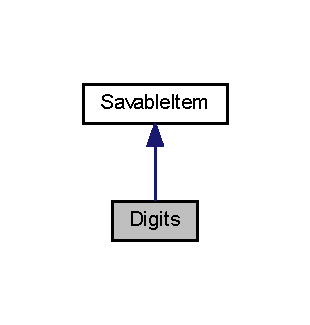
\includegraphics[width=149pt]{class_digits__inherit__graph}
\end{center}
\end{figure}


Граф связей класса Digits\-:
\nopagebreak
\begin{figure}[H]
\begin{center}
\leavevmode
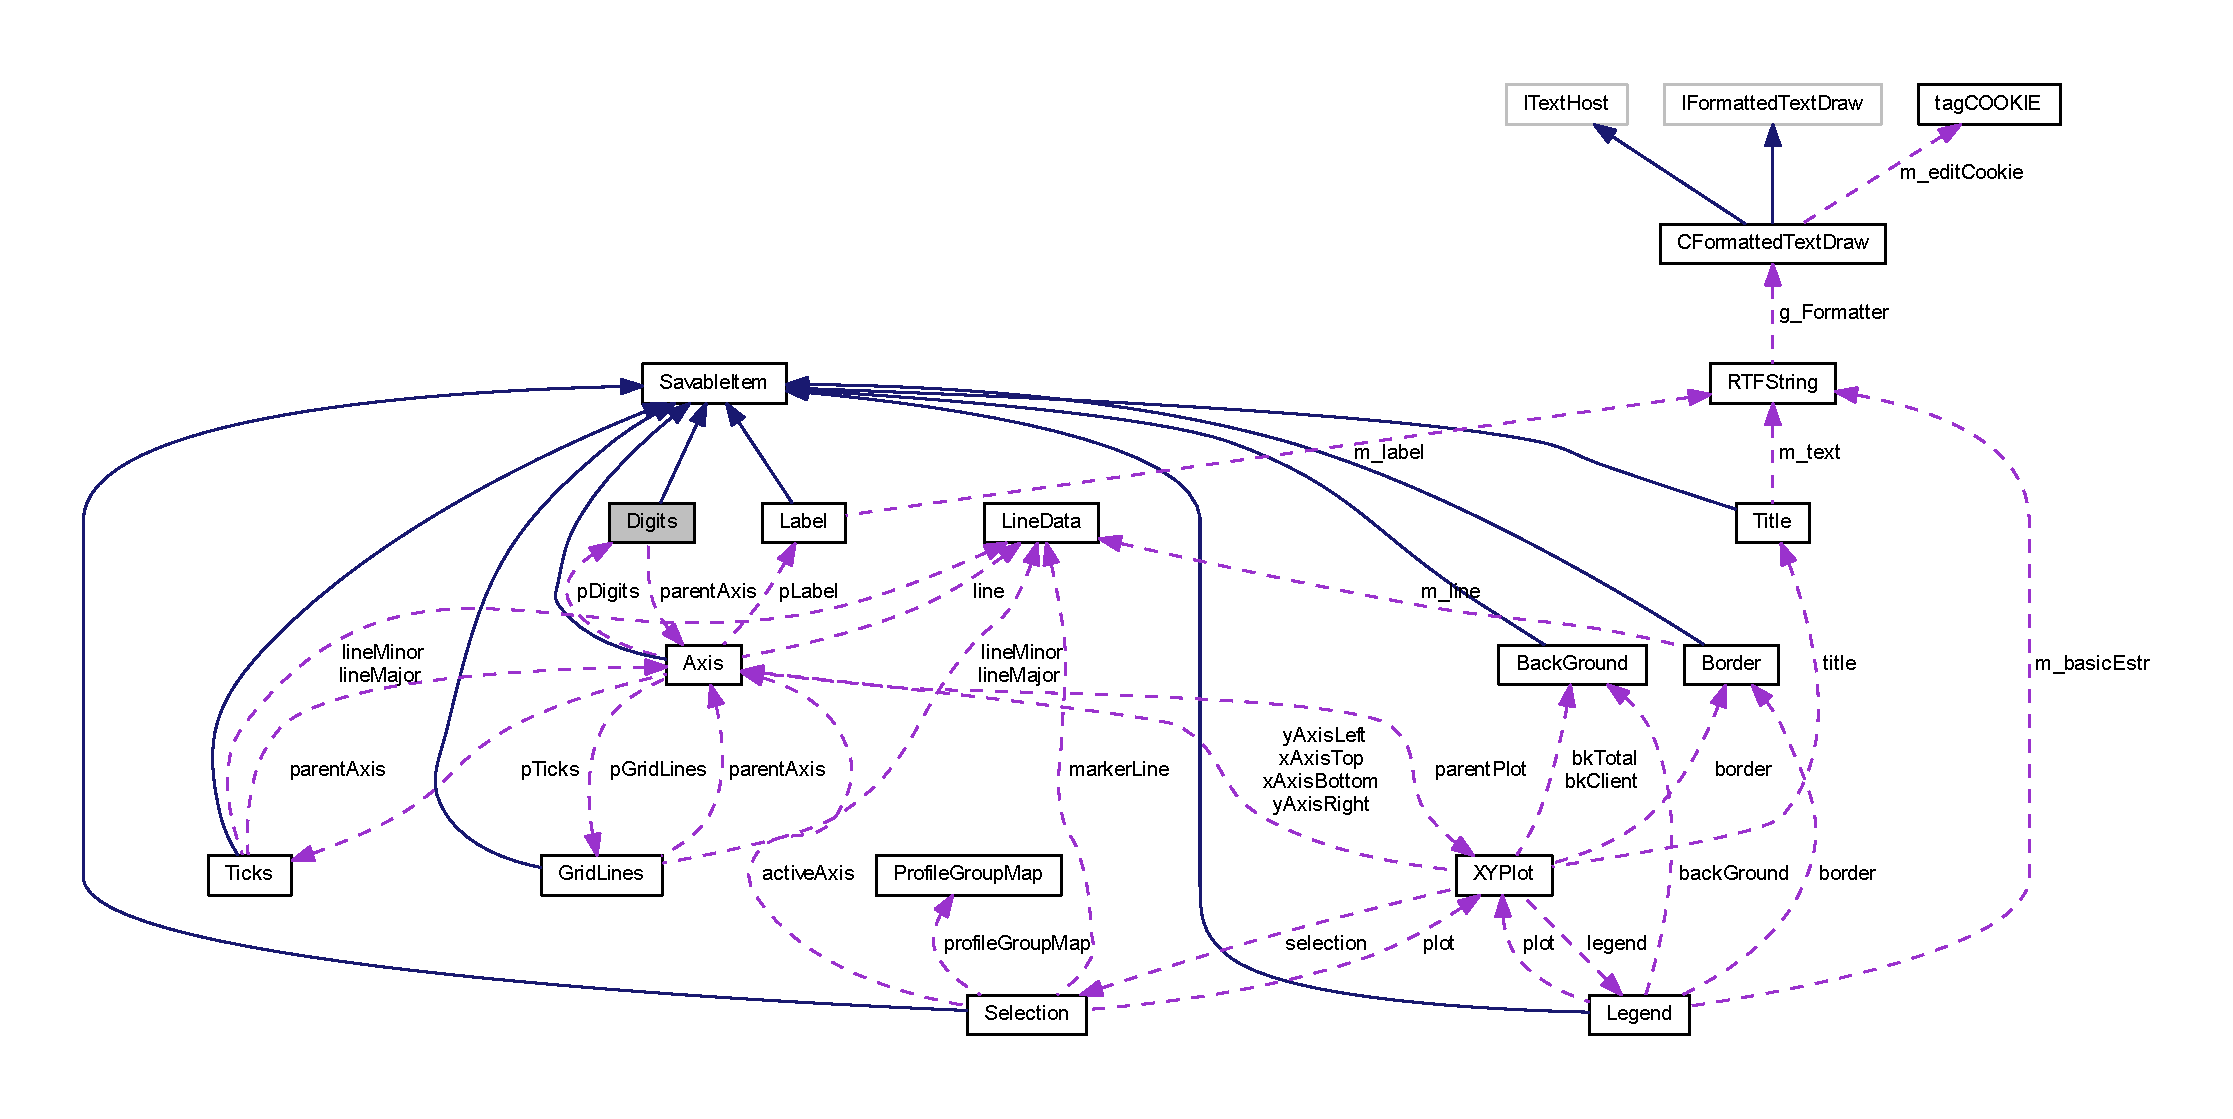
\includegraphics[width=350pt]{class_digits__coll__graph}
\end{center}
\end{figure}
\subsection*{Открытые члены}
\begin{DoxyCompactItemize}
\item 
\hyperlink{class_digits_acd329f27f77896fa7ce6c5e494beaa1c}{Digits} (\hyperlink{class_x_y_plot}{X\-Y\-Plot} $\ast$parent, \hyperlink{class_axis}{Axis} $\ast$\hyperlink{class_digits_a40f4adf8eaf3b89b66adbbccc2099d5d}{parent\-Axis})
\item 
virtual \hyperlink{class_digits_a66e19468f256da28a103894f2ceb9cfe}{$\sim$\-Digits} ()
\item 
void \hyperlink{class_digits_a7d4c1c32b27083457ef094bc7a27ec13}{Set\-Color} (C\-O\-L\-O\-R\-R\-E\-F color, B\-O\-O\-L b\-Major=T\-R\-U\-E)
\item 
C\-O\-L\-O\-R\-R\-E\-F \hyperlink{class_digits_a29d3f2ec295eeebb390bc1eb93b612af}{Get\-Color} (B\-O\-O\-L b\-Major=T\-R\-U\-E) const 
\item 
void \hyperlink{class_digits_ae6c4780ba7c4aba52efff6c8ab353f57}{Set\-Rect} (int left, int top, int right, int bottom)
\item 
void \hyperlink{class_digits_a3c4e4199c39cd5b61f7e9bc23dfb979a}{Set\-Rect} (R\-E\-C\-T self)
\item 
void \hyperlink{class_digits_a6b4c60c397a2c8355dd0a0f31eed1929}{Get\-Rect} (R\-E\-C\-T \&self) const 
\item 
void \hyperlink{class_digits_af74a68f96749f6caf6496b31dacb30e0}{Set\-Template} (std\-::string str\-Template, B\-O\-O\-L b\-Major=T\-R\-U\-E)
\item 
const std\-::string \& \hyperlink{class_digits_aa3072c531d0f83c34cf9e97a5504a43f}{Get\-Template} (B\-O\-O\-L b\-Major=T\-R\-U\-E) const 
\item 
void \hyperlink{class_digits_a06c7cf0b99ff10f9e5d623d62c98426d}{Set\-Font} (const L\-O\-G\-F\-O\-N\-T \&lf, B\-O\-O\-L b\-Major=T\-R\-U\-E)
\item 
void \hyperlink{class_digits_a8cdd43accc18a651207de6c1c8f438c4}{Get\-Font} (L\-O\-G\-F\-O\-N\-T \&lf, B\-O\-O\-L b\-Major=T\-R\-U\-E) const 
\item 
int \hyperlink{class_digits_a7641a9787d3b78bac0425e5597a3e5de}{Calc\-Rect} (H\-D\-C h\-D\-C, R\-E\-C\-T \&rc) const 
\item 
void \hyperlink{class_digits_a9b973868449945e26a10fe3953566d9d}{Enable\-Major} (B\-O\-O\-L enable)
\item 
void \hyperlink{class_digits_a7c34d2810ef21b76b6a301f482b09df3}{Enable\-Minor} (B\-O\-O\-L enable)
\item 
B\-O\-O\-L \hyperlink{class_digits_a0f46d96f7792ffc099ddc4034bb8fe4a}{Is\-Enabled\-Major} () const 
\item 
B\-O\-O\-L \hyperlink{class_digits_af1060dd2a6333c9d1e36942ad5633546}{Is\-Enabled\-Minor} () const 
\item 
int \hyperlink{class_digits_a2a80cf9e4d366d03f4a0902af73af2bc}{Max\-Item\-Length} (H\-D\-C hdc, double fmin, double fmax) const 
\item 
void \hyperlink{class_digits_a8779eafb228a0b7ea0565ebd3198e71c}{Set\-Range} (double f\-Lower, double f\-Upper)
\item 
void \hyperlink{class_digits_ac3ec93b9ed68317ab11ef3a61b69934d}{Get\-Range} (double \&f\-Lower, double \&f\-Upper) const 
\item 
void \hyperlink{class_digits_a3957bbf3699a85811cbbaa01a93fcc88}{Pre\-Draw} (H\-D\-C hdc)
\item 
void \hyperlink{class_digits_ae652ae51841237c43ba06a7b7d5b9a89}{On\-Draw} (H\-D\-C hdc)
\item 
void \hyperlink{class_digits_a4a32dbae6da6819873e0fde7d963cc65}{Optimize\-Ticks} (double \&fmin, double \&fmax, int \&major\-Count, int \&minor\-Count)
\item 
virtual B\-O\-O\-L \hyperlink{class_digits_ad516fc5b9c052a5b0b82469e645a5d0a}{Write} (H\-A\-N\-D\-L\-E h\-File) const 
\item 
virtual B\-O\-O\-L \hyperlink{class_digits_a8e4038efd3b350b447a1d509eaa5040e}{Read} (H\-A\-N\-D\-L\-E h\-File)
\end{DoxyCompactItemize}
\subsection*{Защищенные члены}
\begin{DoxyCompactItemize}
\item 
void \hyperlink{class_digits_acfac4502fbb3122dbb0071af14b71d91}{Push\-Back\-Major} (std\-::string s)
\item 
void \hyperlink{class_digits_ac2f1179123ad83c98480e0ff8e55d12c}{Push\-Back\-Minor} (std\-::string s)
\item 
void \hyperlink{class_digits_ab946e7f29024bc8fda41c286d96958aa}{Beautify} (std\-::string \&s)
\item 
void \hyperlink{class_digits_ae401969abc8fd75f520a00512716a581}{Clear} ()
\end{DoxyCompactItemize}
\subsection*{Защищенные данные}
\begin{DoxyCompactItemize}
\item 
B\-O\-O\-L \hyperlink{class_digits_aaf6398adc6029e62a5b437575e1dc9df}{m\-\_\-enabled\-Major}
\item 
B\-O\-O\-L \hyperlink{class_digits_a3cd58217fb3282ac4e326c3aba8e5014}{m\-\_\-enabled\-Minor}
\item 
int \hyperlink{class_digits_a6363bd7d08bcf1af1f631542007d576b}{offset\-From\-Ticks}
\item 
R\-E\-C\-T \hyperlink{class_digits_ae4aaf160c1fb1a64da858021e376f84b}{m\-\_\-self}
\item 
std\-::string \hyperlink{class_digits_abbe65de11a5be175f825f2727212fe07}{major\-Template}
\item 
std\-::string \hyperlink{class_digits_a6742b3cfd0643d81fea94f4b43bab302}{minor\-Template}
\item 
std\-::vector$<$ std\-::string $>$ \hyperlink{class_digits_a8f37710ae3695963c053ac86907b53c5}{m\-\_\-major\-Digits\-Vector}
\item 
std\-::vector$<$ std\-::string $>$ \hyperlink{class_digits_a2382cd829aa6469431b38f447d9570d8}{m\-\_\-minor\-Digits\-Vector}
\item 
double \hyperlink{class_digits_a086ddfadf3a92ce92096b65841b0a57e}{m\-\_\-f\-Lower}
\item 
double \hyperlink{class_digits_aaadbe21fd0151547ad2aad4dadd82516}{m\-\_\-f\-Upper}
\item 
unsigned \hyperlink{class_digits_ad072b45337ed3492f7798caa246344fe}{n\-Font\-Minor}
\item 
unsigned \hyperlink{class_digits_a7e78c6880a781fef583b8ab06e214c2c}{n\-Font\-Major}
\item 
C\-O\-L\-O\-R\-R\-E\-F \hyperlink{class_digits_ab100cdfd65503955b4d052085c47078a}{cr\-Minor}
\item 
C\-O\-L\-O\-R\-R\-E\-F \hyperlink{class_digits_ae1dbae5da268f81449d27800c19798e6}{cr\-Major}
\item 
\hyperlink{class_axis}{Axis} $\ast$ \hyperlink{class_digits_a40f4adf8eaf3b89b66adbbccc2099d5d}{parent\-Axis}
\end{DoxyCompactItemize}
\subsection*{Дополнительные унаследованные члены}


\subsection{Конструктор(ы)}
\hypertarget{class_digits_acd329f27f77896fa7ce6c5e494beaa1c}{\index{Digits@{Digits}!Digits@{Digits}}
\index{Digits@{Digits}!Digits@{Digits}}
\subsubsection[{Digits}]{\setlength{\rightskip}{0pt plus 5cm}Digits\-::\-Digits (
\begin{DoxyParamCaption}
\item[{{\bf X\-Y\-Plot} $\ast$}]{parent, }
\item[{{\bf Axis} $\ast$}]{parent\-Axis}
\end{DoxyParamCaption}
)}}\label{class_digits_acd329f27f77896fa7ce6c5e494beaa1c}
\hypertarget{class_digits_a66e19468f256da28a103894f2ceb9cfe}{\index{Digits@{Digits}!$\sim$\-Digits@{$\sim$\-Digits}}
\index{$\sim$\-Digits@{$\sim$\-Digits}!Digits@{Digits}}
\subsubsection[{$\sim$\-Digits}]{\setlength{\rightskip}{0pt plus 5cm}Digits\-::$\sim$\-Digits (
\begin{DoxyParamCaption}
{}
\end{DoxyParamCaption}
)\hspace{0.3cm}{\ttfamily [virtual]}}}\label{class_digits_a66e19468f256da28a103894f2ceb9cfe}


\subsection{Методы}
\hypertarget{class_digits_ab946e7f29024bc8fda41c286d96958aa}{\index{Digits@{Digits}!Beautify@{Beautify}}
\index{Beautify@{Beautify}!Digits@{Digits}}
\subsubsection[{Beautify}]{\setlength{\rightskip}{0pt plus 5cm}void Digits\-::\-Beautify (
\begin{DoxyParamCaption}
\item[{std\-::string \&}]{s}
\end{DoxyParamCaption}
)\hspace{0.3cm}{\ttfamily [protected]}}}\label{class_digits_ab946e7f29024bc8fda41c286d96958aa}
\hypertarget{class_digits_a7641a9787d3b78bac0425e5597a3e5de}{\index{Digits@{Digits}!Calc\-Rect@{Calc\-Rect}}
\index{Calc\-Rect@{Calc\-Rect}!Digits@{Digits}}
\subsubsection[{Calc\-Rect}]{\setlength{\rightskip}{0pt plus 5cm}int Digits\-::\-Calc\-Rect (
\begin{DoxyParamCaption}
\item[{H\-D\-C}]{h\-D\-C, }
\item[{R\-E\-C\-T \&}]{rc}
\end{DoxyParamCaption}
) const}}\label{class_digits_a7641a9787d3b78bac0425e5597a3e5de}
\hypertarget{class_digits_ae401969abc8fd75f520a00512716a581}{\index{Digits@{Digits}!Clear@{Clear}}
\index{Clear@{Clear}!Digits@{Digits}}
\subsubsection[{Clear}]{\setlength{\rightskip}{0pt plus 5cm}void Digits\-::\-Clear (
\begin{DoxyParamCaption}
{}
\end{DoxyParamCaption}
)\hspace{0.3cm}{\ttfamily [protected]}}}\label{class_digits_ae401969abc8fd75f520a00512716a581}
\hypertarget{class_digits_a9b973868449945e26a10fe3953566d9d}{\index{Digits@{Digits}!Enable\-Major@{Enable\-Major}}
\index{Enable\-Major@{Enable\-Major}!Digits@{Digits}}
\subsubsection[{Enable\-Major}]{\setlength{\rightskip}{0pt plus 5cm}void Digits\-::\-Enable\-Major (
\begin{DoxyParamCaption}
\item[{B\-O\-O\-L}]{enable}
\end{DoxyParamCaption}
)\hspace{0.3cm}{\ttfamily [inline]}}}\label{class_digits_a9b973868449945e26a10fe3953566d9d}
\hypertarget{class_digits_a7c34d2810ef21b76b6a301f482b09df3}{\index{Digits@{Digits}!Enable\-Minor@{Enable\-Minor}}
\index{Enable\-Minor@{Enable\-Minor}!Digits@{Digits}}
\subsubsection[{Enable\-Minor}]{\setlength{\rightskip}{0pt plus 5cm}void Digits\-::\-Enable\-Minor (
\begin{DoxyParamCaption}
\item[{B\-O\-O\-L}]{enable}
\end{DoxyParamCaption}
)\hspace{0.3cm}{\ttfamily [inline]}}}\label{class_digits_a7c34d2810ef21b76b6a301f482b09df3}
\hypertarget{class_digits_a29d3f2ec295eeebb390bc1eb93b612af}{\index{Digits@{Digits}!Get\-Color@{Get\-Color}}
\index{Get\-Color@{Get\-Color}!Digits@{Digits}}
\subsubsection[{Get\-Color}]{\setlength{\rightskip}{0pt plus 5cm}C\-O\-L\-O\-R\-R\-E\-F Digits\-::\-Get\-Color (
\begin{DoxyParamCaption}
\item[{B\-O\-O\-L}]{b\-Major = {\ttfamily TRUE}}
\end{DoxyParamCaption}
) const}}\label{class_digits_a29d3f2ec295eeebb390bc1eb93b612af}
\hypertarget{class_digits_a8cdd43accc18a651207de6c1c8f438c4}{\index{Digits@{Digits}!Get\-Font@{Get\-Font}}
\index{Get\-Font@{Get\-Font}!Digits@{Digits}}
\subsubsection[{Get\-Font}]{\setlength{\rightskip}{0pt plus 5cm}void Digits\-::\-Get\-Font (
\begin{DoxyParamCaption}
\item[{L\-O\-G\-F\-O\-N\-T \&}]{lf, }
\item[{B\-O\-O\-L}]{b\-Major = {\ttfamily TRUE}}
\end{DoxyParamCaption}
) const}}\label{class_digits_a8cdd43accc18a651207de6c1c8f438c4}
\hypertarget{class_digits_ac3ec93b9ed68317ab11ef3a61b69934d}{\index{Digits@{Digits}!Get\-Range@{Get\-Range}}
\index{Get\-Range@{Get\-Range}!Digits@{Digits}}
\subsubsection[{Get\-Range}]{\setlength{\rightskip}{0pt plus 5cm}void Digits\-::\-Get\-Range (
\begin{DoxyParamCaption}
\item[{double \&}]{f\-Lower, }
\item[{double \&}]{f\-Upper}
\end{DoxyParamCaption}
) const\hspace{0.3cm}{\ttfamily [inline]}}}\label{class_digits_ac3ec93b9ed68317ab11ef3a61b69934d}
\hypertarget{class_digits_a6b4c60c397a2c8355dd0a0f31eed1929}{\index{Digits@{Digits}!Get\-Rect@{Get\-Rect}}
\index{Get\-Rect@{Get\-Rect}!Digits@{Digits}}
\subsubsection[{Get\-Rect}]{\setlength{\rightskip}{0pt plus 5cm}void Digits\-::\-Get\-Rect (
\begin{DoxyParamCaption}
\item[{R\-E\-C\-T \&}]{self}
\end{DoxyParamCaption}
) const\hspace{0.3cm}{\ttfamily [inline]}}}\label{class_digits_a6b4c60c397a2c8355dd0a0f31eed1929}
\hypertarget{class_digits_aa3072c531d0f83c34cf9e97a5504a43f}{\index{Digits@{Digits}!Get\-Template@{Get\-Template}}
\index{Get\-Template@{Get\-Template}!Digits@{Digits}}
\subsubsection[{Get\-Template}]{\setlength{\rightskip}{0pt plus 5cm}const std\-::string \& Digits\-::\-Get\-Template (
\begin{DoxyParamCaption}
\item[{B\-O\-O\-L}]{b\-Major = {\ttfamily TRUE}}
\end{DoxyParamCaption}
) const}}\label{class_digits_aa3072c531d0f83c34cf9e97a5504a43f}
\hypertarget{class_digits_a0f46d96f7792ffc099ddc4034bb8fe4a}{\index{Digits@{Digits}!Is\-Enabled\-Major@{Is\-Enabled\-Major}}
\index{Is\-Enabled\-Major@{Is\-Enabled\-Major}!Digits@{Digits}}
\subsubsection[{Is\-Enabled\-Major}]{\setlength{\rightskip}{0pt plus 5cm}B\-O\-O\-L Digits\-::\-Is\-Enabled\-Major (
\begin{DoxyParamCaption}
{}
\end{DoxyParamCaption}
) const\hspace{0.3cm}{\ttfamily [inline]}}}\label{class_digits_a0f46d96f7792ffc099ddc4034bb8fe4a}
\hypertarget{class_digits_af1060dd2a6333c9d1e36942ad5633546}{\index{Digits@{Digits}!Is\-Enabled\-Minor@{Is\-Enabled\-Minor}}
\index{Is\-Enabled\-Minor@{Is\-Enabled\-Minor}!Digits@{Digits}}
\subsubsection[{Is\-Enabled\-Minor}]{\setlength{\rightskip}{0pt plus 5cm}B\-O\-O\-L Digits\-::\-Is\-Enabled\-Minor (
\begin{DoxyParamCaption}
{}
\end{DoxyParamCaption}
) const\hspace{0.3cm}{\ttfamily [inline]}}}\label{class_digits_af1060dd2a6333c9d1e36942ad5633546}
\hypertarget{class_digits_a2a80cf9e4d366d03f4a0902af73af2bc}{\index{Digits@{Digits}!Max\-Item\-Length@{Max\-Item\-Length}}
\index{Max\-Item\-Length@{Max\-Item\-Length}!Digits@{Digits}}
\subsubsection[{Max\-Item\-Length}]{\setlength{\rightskip}{0pt plus 5cm}int Digits\-::\-Max\-Item\-Length (
\begin{DoxyParamCaption}
\item[{H\-D\-C}]{hdc, }
\item[{double}]{fmin, }
\item[{double}]{fmax}
\end{DoxyParamCaption}
) const}}\label{class_digits_a2a80cf9e4d366d03f4a0902af73af2bc}
\hypertarget{class_digits_ae652ae51841237c43ba06a7b7d5b9a89}{\index{Digits@{Digits}!On\-Draw@{On\-Draw}}
\index{On\-Draw@{On\-Draw}!Digits@{Digits}}
\subsubsection[{On\-Draw}]{\setlength{\rightskip}{0pt plus 5cm}void Digits\-::\-On\-Draw (
\begin{DoxyParamCaption}
\item[{H\-D\-C}]{hdc}
\end{DoxyParamCaption}
)}}\label{class_digits_ae652ae51841237c43ba06a7b7d5b9a89}
\hypertarget{class_digits_a4a32dbae6da6819873e0fde7d963cc65}{\index{Digits@{Digits}!Optimize\-Ticks@{Optimize\-Ticks}}
\index{Optimize\-Ticks@{Optimize\-Ticks}!Digits@{Digits}}
\subsubsection[{Optimize\-Ticks}]{\setlength{\rightskip}{0pt plus 5cm}void Digits\-::\-Optimize\-Ticks (
\begin{DoxyParamCaption}
\item[{double \&}]{fmin, }
\item[{double \&}]{fmax, }
\item[{int \&}]{major\-Count, }
\item[{int \&}]{minor\-Count}
\end{DoxyParamCaption}
)}}\label{class_digits_a4a32dbae6da6819873e0fde7d963cc65}
\hypertarget{class_digits_a3957bbf3699a85811cbbaa01a93fcc88}{\index{Digits@{Digits}!Pre\-Draw@{Pre\-Draw}}
\index{Pre\-Draw@{Pre\-Draw}!Digits@{Digits}}
\subsubsection[{Pre\-Draw}]{\setlength{\rightskip}{0pt plus 5cm}void Digits\-::\-Pre\-Draw (
\begin{DoxyParamCaption}
\item[{H\-D\-C}]{hdc}
\end{DoxyParamCaption}
)}}\label{class_digits_a3957bbf3699a85811cbbaa01a93fcc88}
\hypertarget{class_digits_acfac4502fbb3122dbb0071af14b71d91}{\index{Digits@{Digits}!Push\-Back\-Major@{Push\-Back\-Major}}
\index{Push\-Back\-Major@{Push\-Back\-Major}!Digits@{Digits}}
\subsubsection[{Push\-Back\-Major}]{\setlength{\rightskip}{0pt plus 5cm}void Digits\-::\-Push\-Back\-Major (
\begin{DoxyParamCaption}
\item[{std\-::string}]{s}
\end{DoxyParamCaption}
)\hspace{0.3cm}{\ttfamily [protected]}}}\label{class_digits_acfac4502fbb3122dbb0071af14b71d91}
\hypertarget{class_digits_ac2f1179123ad83c98480e0ff8e55d12c}{\index{Digits@{Digits}!Push\-Back\-Minor@{Push\-Back\-Minor}}
\index{Push\-Back\-Minor@{Push\-Back\-Minor}!Digits@{Digits}}
\subsubsection[{Push\-Back\-Minor}]{\setlength{\rightskip}{0pt plus 5cm}void Digits\-::\-Push\-Back\-Minor (
\begin{DoxyParamCaption}
\item[{std\-::string}]{s}
\end{DoxyParamCaption}
)\hspace{0.3cm}{\ttfamily [protected]}}}\label{class_digits_ac2f1179123ad83c98480e0ff8e55d12c}
\hypertarget{class_digits_a8e4038efd3b350b447a1d509eaa5040e}{\index{Digits@{Digits}!Read@{Read}}
\index{Read@{Read}!Digits@{Digits}}
\subsubsection[{Read}]{\setlength{\rightskip}{0pt plus 5cm}B\-O\-O\-L Digits\-::\-Read (
\begin{DoxyParamCaption}
\item[{H\-A\-N\-D\-L\-E}]{h\-File}
\end{DoxyParamCaption}
)\hspace{0.3cm}{\ttfamily [virtual]}}}\label{class_digits_a8e4038efd3b350b447a1d509eaa5040e}


Замещает \hyperlink{class_savable_item_a7eadd16b2cb0652091cc15f596a00fb2}{Savable\-Item}.

\hypertarget{class_digits_a7d4c1c32b27083457ef094bc7a27ec13}{\index{Digits@{Digits}!Set\-Color@{Set\-Color}}
\index{Set\-Color@{Set\-Color}!Digits@{Digits}}
\subsubsection[{Set\-Color}]{\setlength{\rightskip}{0pt plus 5cm}void Digits\-::\-Set\-Color (
\begin{DoxyParamCaption}
\item[{C\-O\-L\-O\-R\-R\-E\-F}]{color, }
\item[{B\-O\-O\-L}]{b\-Major = {\ttfamily TRUE}}
\end{DoxyParamCaption}
)}}\label{class_digits_a7d4c1c32b27083457ef094bc7a27ec13}
\hypertarget{class_digits_a06c7cf0b99ff10f9e5d623d62c98426d}{\index{Digits@{Digits}!Set\-Font@{Set\-Font}}
\index{Set\-Font@{Set\-Font}!Digits@{Digits}}
\subsubsection[{Set\-Font}]{\setlength{\rightskip}{0pt plus 5cm}void Digits\-::\-Set\-Font (
\begin{DoxyParamCaption}
\item[{const L\-O\-G\-F\-O\-N\-T \&}]{lf, }
\item[{B\-O\-O\-L}]{b\-Major = {\ttfamily TRUE}}
\end{DoxyParamCaption}
)}}\label{class_digits_a06c7cf0b99ff10f9e5d623d62c98426d}
\hypertarget{class_digits_a8779eafb228a0b7ea0565ebd3198e71c}{\index{Digits@{Digits}!Set\-Range@{Set\-Range}}
\index{Set\-Range@{Set\-Range}!Digits@{Digits}}
\subsubsection[{Set\-Range}]{\setlength{\rightskip}{0pt plus 5cm}void Digits\-::\-Set\-Range (
\begin{DoxyParamCaption}
\item[{double}]{f\-Lower, }
\item[{double}]{f\-Upper}
\end{DoxyParamCaption}
)\hspace{0.3cm}{\ttfamily [inline]}}}\label{class_digits_a8779eafb228a0b7ea0565ebd3198e71c}
\hypertarget{class_digits_ae6c4780ba7c4aba52efff6c8ab353f57}{\index{Digits@{Digits}!Set\-Rect@{Set\-Rect}}
\index{Set\-Rect@{Set\-Rect}!Digits@{Digits}}
\subsubsection[{Set\-Rect}]{\setlength{\rightskip}{0pt plus 5cm}void Digits\-::\-Set\-Rect (
\begin{DoxyParamCaption}
\item[{int}]{left, }
\item[{int}]{top, }
\item[{int}]{right, }
\item[{int}]{bottom}
\end{DoxyParamCaption}
)}}\label{class_digits_ae6c4780ba7c4aba52efff6c8ab353f57}
\hypertarget{class_digits_a3c4e4199c39cd5b61f7e9bc23dfb979a}{\index{Digits@{Digits}!Set\-Rect@{Set\-Rect}}
\index{Set\-Rect@{Set\-Rect}!Digits@{Digits}}
\subsubsection[{Set\-Rect}]{\setlength{\rightskip}{0pt plus 5cm}void Digits\-::\-Set\-Rect (
\begin{DoxyParamCaption}
\item[{R\-E\-C\-T}]{self}
\end{DoxyParamCaption}
)\hspace{0.3cm}{\ttfamily [inline]}}}\label{class_digits_a3c4e4199c39cd5b61f7e9bc23dfb979a}
\hypertarget{class_digits_af74a68f96749f6caf6496b31dacb30e0}{\index{Digits@{Digits}!Set\-Template@{Set\-Template}}
\index{Set\-Template@{Set\-Template}!Digits@{Digits}}
\subsubsection[{Set\-Template}]{\setlength{\rightskip}{0pt plus 5cm}void Digits\-::\-Set\-Template (
\begin{DoxyParamCaption}
\item[{std\-::string}]{str\-Template, }
\item[{B\-O\-O\-L}]{b\-Major = {\ttfamily TRUE}}
\end{DoxyParamCaption}
)}}\label{class_digits_af74a68f96749f6caf6496b31dacb30e0}
\hypertarget{class_digits_ad516fc5b9c052a5b0b82469e645a5d0a}{\index{Digits@{Digits}!Write@{Write}}
\index{Write@{Write}!Digits@{Digits}}
\subsubsection[{Write}]{\setlength{\rightskip}{0pt plus 5cm}B\-O\-O\-L Digits\-::\-Write (
\begin{DoxyParamCaption}
\item[{H\-A\-N\-D\-L\-E}]{h\-File}
\end{DoxyParamCaption}
) const\hspace{0.3cm}{\ttfamily [virtual]}}}\label{class_digits_ad516fc5b9c052a5b0b82469e645a5d0a}


Замещает \hyperlink{class_savable_item_a0da511a4854f515096f8f9b498f64158}{Savable\-Item}.



\subsection{Данные класса}
\hypertarget{class_digits_ae1dbae5da268f81449d27800c19798e6}{\index{Digits@{Digits}!cr\-Major@{cr\-Major}}
\index{cr\-Major@{cr\-Major}!Digits@{Digits}}
\subsubsection[{cr\-Major}]{\setlength{\rightskip}{0pt plus 5cm}C\-O\-L\-O\-R\-R\-E\-F Digits\-::cr\-Major\hspace{0.3cm}{\ttfamily [protected]}}}\label{class_digits_ae1dbae5da268f81449d27800c19798e6}
\hypertarget{class_digits_ab100cdfd65503955b4d052085c47078a}{\index{Digits@{Digits}!cr\-Minor@{cr\-Minor}}
\index{cr\-Minor@{cr\-Minor}!Digits@{Digits}}
\subsubsection[{cr\-Minor}]{\setlength{\rightskip}{0pt plus 5cm}C\-O\-L\-O\-R\-R\-E\-F Digits\-::cr\-Minor\hspace{0.3cm}{\ttfamily [protected]}}}\label{class_digits_ab100cdfd65503955b4d052085c47078a}
\hypertarget{class_digits_aaf6398adc6029e62a5b437575e1dc9df}{\index{Digits@{Digits}!m\-\_\-enabled\-Major@{m\-\_\-enabled\-Major}}
\index{m\-\_\-enabled\-Major@{m\-\_\-enabled\-Major}!Digits@{Digits}}
\subsubsection[{m\-\_\-enabled\-Major}]{\setlength{\rightskip}{0pt plus 5cm}B\-O\-O\-L Digits\-::m\-\_\-enabled\-Major\hspace{0.3cm}{\ttfamily [protected]}}}\label{class_digits_aaf6398adc6029e62a5b437575e1dc9df}
\hypertarget{class_digits_a3cd58217fb3282ac4e326c3aba8e5014}{\index{Digits@{Digits}!m\-\_\-enabled\-Minor@{m\-\_\-enabled\-Minor}}
\index{m\-\_\-enabled\-Minor@{m\-\_\-enabled\-Minor}!Digits@{Digits}}
\subsubsection[{m\-\_\-enabled\-Minor}]{\setlength{\rightskip}{0pt plus 5cm}B\-O\-O\-L Digits\-::m\-\_\-enabled\-Minor\hspace{0.3cm}{\ttfamily [protected]}}}\label{class_digits_a3cd58217fb3282ac4e326c3aba8e5014}
\hypertarget{class_digits_a086ddfadf3a92ce92096b65841b0a57e}{\index{Digits@{Digits}!m\-\_\-f\-Lower@{m\-\_\-f\-Lower}}
\index{m\-\_\-f\-Lower@{m\-\_\-f\-Lower}!Digits@{Digits}}
\subsubsection[{m\-\_\-f\-Lower}]{\setlength{\rightskip}{0pt plus 5cm}double Digits\-::m\-\_\-f\-Lower\hspace{0.3cm}{\ttfamily [protected]}}}\label{class_digits_a086ddfadf3a92ce92096b65841b0a57e}
\hypertarget{class_digits_aaadbe21fd0151547ad2aad4dadd82516}{\index{Digits@{Digits}!m\-\_\-f\-Upper@{m\-\_\-f\-Upper}}
\index{m\-\_\-f\-Upper@{m\-\_\-f\-Upper}!Digits@{Digits}}
\subsubsection[{m\-\_\-f\-Upper}]{\setlength{\rightskip}{0pt plus 5cm}double Digits\-::m\-\_\-f\-Upper\hspace{0.3cm}{\ttfamily [protected]}}}\label{class_digits_aaadbe21fd0151547ad2aad4dadd82516}
\hypertarget{class_digits_a8f37710ae3695963c053ac86907b53c5}{\index{Digits@{Digits}!m\-\_\-major\-Digits\-Vector@{m\-\_\-major\-Digits\-Vector}}
\index{m\-\_\-major\-Digits\-Vector@{m\-\_\-major\-Digits\-Vector}!Digits@{Digits}}
\subsubsection[{m\-\_\-major\-Digits\-Vector}]{\setlength{\rightskip}{0pt plus 5cm}std\-::vector$<$ std\-::string $>$ Digits\-::m\-\_\-major\-Digits\-Vector\hspace{0.3cm}{\ttfamily [protected]}}}\label{class_digits_a8f37710ae3695963c053ac86907b53c5}
\hypertarget{class_digits_a2382cd829aa6469431b38f447d9570d8}{\index{Digits@{Digits}!m\-\_\-minor\-Digits\-Vector@{m\-\_\-minor\-Digits\-Vector}}
\index{m\-\_\-minor\-Digits\-Vector@{m\-\_\-minor\-Digits\-Vector}!Digits@{Digits}}
\subsubsection[{m\-\_\-minor\-Digits\-Vector}]{\setlength{\rightskip}{0pt plus 5cm}std\-::vector$<$ std\-::string $>$ Digits\-::m\-\_\-minor\-Digits\-Vector\hspace{0.3cm}{\ttfamily [protected]}}}\label{class_digits_a2382cd829aa6469431b38f447d9570d8}
\hypertarget{class_digits_ae4aaf160c1fb1a64da858021e376f84b}{\index{Digits@{Digits}!m\-\_\-self@{m\-\_\-self}}
\index{m\-\_\-self@{m\-\_\-self}!Digits@{Digits}}
\subsubsection[{m\-\_\-self}]{\setlength{\rightskip}{0pt plus 5cm}R\-E\-C\-T Digits\-::m\-\_\-self\hspace{0.3cm}{\ttfamily [protected]}}}\label{class_digits_ae4aaf160c1fb1a64da858021e376f84b}
\hypertarget{class_digits_abbe65de11a5be175f825f2727212fe07}{\index{Digits@{Digits}!major\-Template@{major\-Template}}
\index{major\-Template@{major\-Template}!Digits@{Digits}}
\subsubsection[{major\-Template}]{\setlength{\rightskip}{0pt plus 5cm}std\-::string Digits\-::major\-Template\hspace{0.3cm}{\ttfamily [protected]}}}\label{class_digits_abbe65de11a5be175f825f2727212fe07}
\hypertarget{class_digits_a6742b3cfd0643d81fea94f4b43bab302}{\index{Digits@{Digits}!minor\-Template@{minor\-Template}}
\index{minor\-Template@{minor\-Template}!Digits@{Digits}}
\subsubsection[{minor\-Template}]{\setlength{\rightskip}{0pt plus 5cm}std\-::string Digits\-::minor\-Template\hspace{0.3cm}{\ttfamily [protected]}}}\label{class_digits_a6742b3cfd0643d81fea94f4b43bab302}
\hypertarget{class_digits_a7e78c6880a781fef583b8ab06e214c2c}{\index{Digits@{Digits}!n\-Font\-Major@{n\-Font\-Major}}
\index{n\-Font\-Major@{n\-Font\-Major}!Digits@{Digits}}
\subsubsection[{n\-Font\-Major}]{\setlength{\rightskip}{0pt plus 5cm}unsigned Digits\-::n\-Font\-Major\hspace{0.3cm}{\ttfamily [protected]}}}\label{class_digits_a7e78c6880a781fef583b8ab06e214c2c}
\hypertarget{class_digits_ad072b45337ed3492f7798caa246344fe}{\index{Digits@{Digits}!n\-Font\-Minor@{n\-Font\-Minor}}
\index{n\-Font\-Minor@{n\-Font\-Minor}!Digits@{Digits}}
\subsubsection[{n\-Font\-Minor}]{\setlength{\rightskip}{0pt plus 5cm}unsigned Digits\-::n\-Font\-Minor\hspace{0.3cm}{\ttfamily [protected]}}}\label{class_digits_ad072b45337ed3492f7798caa246344fe}
\hypertarget{class_digits_a6363bd7d08bcf1af1f631542007d576b}{\index{Digits@{Digits}!offset\-From\-Ticks@{offset\-From\-Ticks}}
\index{offset\-From\-Ticks@{offset\-From\-Ticks}!Digits@{Digits}}
\subsubsection[{offset\-From\-Ticks}]{\setlength{\rightskip}{0pt plus 5cm}int Digits\-::offset\-From\-Ticks\hspace{0.3cm}{\ttfamily [protected]}}}\label{class_digits_a6363bd7d08bcf1af1f631542007d576b}
\hypertarget{class_digits_a40f4adf8eaf3b89b66adbbccc2099d5d}{\index{Digits@{Digits}!parent\-Axis@{parent\-Axis}}
\index{parent\-Axis@{parent\-Axis}!Digits@{Digits}}
\subsubsection[{parent\-Axis}]{\setlength{\rightskip}{0pt plus 5cm}{\bf Axis}$\ast$ Digits\-::parent\-Axis\hspace{0.3cm}{\ttfamily [protected]}}}\label{class_digits_a40f4adf8eaf3b89b66adbbccc2099d5d}


Объявления и описания членов классов находятся в файлах\-:\begin{DoxyCompactItemize}
\item 
src/\hyperlink{digits_8h}{digits.\-h}\item 
src/\hyperlink{digits_8cpp}{digits.\-cpp}\end{DoxyCompactItemize}

\hypertarget{classdnp__checkout_1_1dnp__checkout__failure}{\section{Класс dnp\-\_\-checkout\-:\-:dnp\-\_\-checkout\-\_\-failure}
\label{classdnp__checkout_1_1dnp__checkout__failure}\index{dnp\-\_\-checkout\-::dnp\-\_\-checkout\-\_\-failure@{dnp\-\_\-checkout\-::dnp\-\_\-checkout\-\_\-failure}}
}


{\ttfamily \#include $<$dnp\-\_\-checkout.\-h$>$}

\subsection*{Открытые члены}
\begin{DoxyCompactItemize}
\item 
\hyperlink{classdnp__checkout_1_1dnp__checkout__failure_a5a27266473431c67a61c3d172a8fad04}{dnp\-\_\-checkout\-\_\-failure} ()
\end{DoxyCompactItemize}


\subsection{Конструктор(ы)}
\hypertarget{classdnp__checkout_1_1dnp__checkout__failure_a5a27266473431c67a61c3d172a8fad04}{\index{dnp\-\_\-checkout\-::dnp\-\_\-checkout\-\_\-failure@{dnp\-\_\-checkout\-::dnp\-\_\-checkout\-\_\-failure}!dnp\-\_\-checkout\-\_\-failure@{dnp\-\_\-checkout\-\_\-failure}}
\index{dnp\-\_\-checkout\-\_\-failure@{dnp\-\_\-checkout\-\_\-failure}!dnp_checkout::dnp_checkout_failure@{dnp\-\_\-checkout\-::dnp\-\_\-checkout\-\_\-failure}}
\subsubsection[{dnp\-\_\-checkout\-\_\-failure}]{\setlength{\rightskip}{0pt plus 5cm}dnp\-\_\-checkout\-::dnp\-\_\-checkout\-\_\-failure\-::dnp\-\_\-checkout\-\_\-failure (
\begin{DoxyParamCaption}
{}
\end{DoxyParamCaption}
)\hspace{0.3cm}{\ttfamily [inline]}}}\label{classdnp__checkout_1_1dnp__checkout__failure_a5a27266473431c67a61c3d172a8fad04}


Объявления и описания членов класса находятся в файле\-:\begin{DoxyCompactItemize}
\item 
src/\hyperlink{dnp__checkout_8h}{dnp\-\_\-checkout.\-h}\end{DoxyCompactItemize}

\hypertarget{class_font_manager}{\section{Класс Font\-Manager}
\label{class_font_manager}\index{Font\-Manager@{Font\-Manager}}
}


{\ttfamily \#include $<$fontmanager.\-h$>$}

\subsection*{Классы}
\begin{DoxyCompactItemize}
\item 
struct \hyperlink{struct_font_manager_1_1lf__less}{lf\-\_\-less}
\end{DoxyCompactItemize}
\subsection*{Открытые члены}
\begin{DoxyCompactItemize}
\item 
unsigned \hyperlink{class_font_manager_a51482f94502a104c3082d8c117fafb1f}{Register\-Font} (const L\-O\-G\-F\-O\-N\-T \&lf)
\item 
H\-F\-O\-N\-T \hyperlink{class_font_manager_a9cbab3da5aed9d27472d67bc3568d278}{Get\-Font} (unsigned index)
\item 
unsigned \hyperlink{class_font_manager_a83c76cdbcc38cd3e27b85642c7ef133d}{Size} () const 
\item 
\hyperlink{class_font_manager_aa190bb023b4cf2ad28e24c69ef57f380}{$\sim$\-Font\-Manager} ()
\end{DoxyCompactItemize}
\subsection*{Открытые статические члены}
\begin{DoxyCompactItemize}
\item 
static \hyperlink{class_font_manager}{Font\-Manager} \& \hyperlink{class_font_manager_a2e6285874d17832e06eb4c66479ec6bf}{Instance} ()
\end{DoxyCompactItemize}
\subsection*{Защищенные типы}
\begin{DoxyCompactItemize}
\item 
typedef std\-::map$<$ const \\*
L\-O\-G\-F\-O\-N\-T, int, \hyperlink{struct_font_manager_1_1lf__less}{lf\-\_\-less} $>$ \hyperlink{class_font_manager_a053e5dac54d91800c691c093e191d17c}{Logfont\-Map}
\item 
typedef std\-::pair$<$ H\-F\-O\-N\-T, \\*
const L\-O\-G\-F\-O\-N\-T $\ast$const  $>$ \hyperlink{class_font_manager_ae5b94ccffd33a60792fc6a2731e48e5f}{Hfont\-Logfont\-Pair}
\end{DoxyCompactItemize}
\subsection*{Защищенные члены}
\begin{DoxyCompactItemize}
\item 
\hyperlink{class_font_manager_a2f89acd28b5bd24e747aacd3208131ef}{Font\-Manager} ()
\end{DoxyCompactItemize}
\subsection*{Защищенные данные}
\begin{DoxyCompactItemize}
\item 
\hyperlink{class_font_manager_a053e5dac54d91800c691c093e191d17c}{Logfont\-Map} \hyperlink{class_font_manager_a8834f43163db4be815db7a2cb236a36e}{logfont\-Map}
\item 
std\-::vector$<$ \hyperlink{class_font_manager_ae5b94ccffd33a60792fc6a2731e48e5f}{Hfont\-Logfont\-Pair} $>$ \hyperlink{class_font_manager_aa50d6f013a9f72cc63a33370a5ee87d7}{font\-Pair\-Vector}
\item 
C\-R\-I\-T\-I\-C\-A\-L\-\_\-\-S\-E\-C\-T\-I\-O\-N \hyperlink{class_font_manager_ae59f42d519931bb99c3a1caaf7d560c0}{m\-\_\-cs}
\end{DoxyCompactItemize}


\subsection{Определения типов}
\hypertarget{class_font_manager_ae5b94ccffd33a60792fc6a2731e48e5f}{\index{Font\-Manager@{Font\-Manager}!Hfont\-Logfont\-Pair@{Hfont\-Logfont\-Pair}}
\index{Hfont\-Logfont\-Pair@{Hfont\-Logfont\-Pair}!FontManager@{Font\-Manager}}
\subsubsection[{Hfont\-Logfont\-Pair}]{\setlength{\rightskip}{0pt plus 5cm}typedef std\-::pair$<$ H\-F\-O\-N\-T, const L\-O\-G\-F\-O\-N\-T$\ast$ const $>$ {\bf Font\-Manager\-::\-Hfont\-Logfont\-Pair}\hspace{0.3cm}{\ttfamily [protected]}}}\label{class_font_manager_ae5b94ccffd33a60792fc6a2731e48e5f}
\hypertarget{class_font_manager_a053e5dac54d91800c691c093e191d17c}{\index{Font\-Manager@{Font\-Manager}!Logfont\-Map@{Logfont\-Map}}
\index{Logfont\-Map@{Logfont\-Map}!FontManager@{Font\-Manager}}
\subsubsection[{Logfont\-Map}]{\setlength{\rightskip}{0pt plus 5cm}typedef std\-::map$<$ const L\-O\-G\-F\-O\-N\-T, int, {\bf lf\-\_\-less} $>$ {\bf Font\-Manager\-::\-Logfont\-Map}\hspace{0.3cm}{\ttfamily [protected]}}}\label{class_font_manager_a053e5dac54d91800c691c093e191d17c}


\subsection{Конструктор(ы)}
\hypertarget{class_font_manager_aa190bb023b4cf2ad28e24c69ef57f380}{\index{Font\-Manager@{Font\-Manager}!$\sim$\-Font\-Manager@{$\sim$\-Font\-Manager}}
\index{$\sim$\-Font\-Manager@{$\sim$\-Font\-Manager}!FontManager@{Font\-Manager}}
\subsubsection[{$\sim$\-Font\-Manager}]{\setlength{\rightskip}{0pt plus 5cm}Font\-Manager\-::$\sim$\-Font\-Manager (
\begin{DoxyParamCaption}
{}
\end{DoxyParamCaption}
)\hspace{0.3cm}{\ttfamily [inline]}}}\label{class_font_manager_aa190bb023b4cf2ad28e24c69ef57f380}
\hypertarget{class_font_manager_a2f89acd28b5bd24e747aacd3208131ef}{\index{Font\-Manager@{Font\-Manager}!Font\-Manager@{Font\-Manager}}
\index{Font\-Manager@{Font\-Manager}!FontManager@{Font\-Manager}}
\subsubsection[{Font\-Manager}]{\setlength{\rightskip}{0pt plus 5cm}Font\-Manager\-::\-Font\-Manager (
\begin{DoxyParamCaption}
{}
\end{DoxyParamCaption}
)\hspace{0.3cm}{\ttfamily [inline]}, {\ttfamily [protected]}}}\label{class_font_manager_a2f89acd28b5bd24e747aacd3208131ef}


\subsection{Методы}
\hypertarget{class_font_manager_a9cbab3da5aed9d27472d67bc3568d278}{\index{Font\-Manager@{Font\-Manager}!Get\-Font@{Get\-Font}}
\index{Get\-Font@{Get\-Font}!FontManager@{Font\-Manager}}
\subsubsection[{Get\-Font}]{\setlength{\rightskip}{0pt plus 5cm}H\-F\-O\-N\-T Font\-Manager\-::\-Get\-Font (
\begin{DoxyParamCaption}
\item[{unsigned}]{index}
\end{DoxyParamCaption}
)\hspace{0.3cm}{\ttfamily [inline]}}}\label{class_font_manager_a9cbab3da5aed9d27472d67bc3568d278}
\hypertarget{class_font_manager_a2e6285874d17832e06eb4c66479ec6bf}{\index{Font\-Manager@{Font\-Manager}!Instance@{Instance}}
\index{Instance@{Instance}!FontManager@{Font\-Manager}}
\subsubsection[{Instance}]{\setlength{\rightskip}{0pt plus 5cm}static {\bf Font\-Manager}\& Font\-Manager\-::\-Instance (
\begin{DoxyParamCaption}
{}
\end{DoxyParamCaption}
)\hspace{0.3cm}{\ttfamily [inline]}, {\ttfamily [static]}}}\label{class_font_manager_a2e6285874d17832e06eb4c66479ec6bf}
\hypertarget{class_font_manager_a51482f94502a104c3082d8c117fafb1f}{\index{Font\-Manager@{Font\-Manager}!Register\-Font@{Register\-Font}}
\index{Register\-Font@{Register\-Font}!FontManager@{Font\-Manager}}
\subsubsection[{Register\-Font}]{\setlength{\rightskip}{0pt plus 5cm}unsigned Font\-Manager\-::\-Register\-Font (
\begin{DoxyParamCaption}
\item[{const L\-O\-G\-F\-O\-N\-T \&}]{lf}
\end{DoxyParamCaption}
)\hspace{0.3cm}{\ttfamily [inline]}}}\label{class_font_manager_a51482f94502a104c3082d8c117fafb1f}
\hypertarget{class_font_manager_a83c76cdbcc38cd3e27b85642c7ef133d}{\index{Font\-Manager@{Font\-Manager}!Size@{Size}}
\index{Size@{Size}!FontManager@{Font\-Manager}}
\subsubsection[{Size}]{\setlength{\rightskip}{0pt plus 5cm}unsigned Font\-Manager\-::\-Size (
\begin{DoxyParamCaption}
{}
\end{DoxyParamCaption}
) const\hspace{0.3cm}{\ttfamily [inline]}}}\label{class_font_manager_a83c76cdbcc38cd3e27b85642c7ef133d}


\subsection{Данные класса}
\hypertarget{class_font_manager_aa50d6f013a9f72cc63a33370a5ee87d7}{\index{Font\-Manager@{Font\-Manager}!font\-Pair\-Vector@{font\-Pair\-Vector}}
\index{font\-Pair\-Vector@{font\-Pair\-Vector}!FontManager@{Font\-Manager}}
\subsubsection[{font\-Pair\-Vector}]{\setlength{\rightskip}{0pt plus 5cm}std\-::vector$<$ {\bf Hfont\-Logfont\-Pair} $>$ Font\-Manager\-::font\-Pair\-Vector\hspace{0.3cm}{\ttfamily [protected]}}}\label{class_font_manager_aa50d6f013a9f72cc63a33370a5ee87d7}
\hypertarget{class_font_manager_a8834f43163db4be815db7a2cb236a36e}{\index{Font\-Manager@{Font\-Manager}!logfont\-Map@{logfont\-Map}}
\index{logfont\-Map@{logfont\-Map}!FontManager@{Font\-Manager}}
\subsubsection[{logfont\-Map}]{\setlength{\rightskip}{0pt plus 5cm}{\bf Logfont\-Map} Font\-Manager\-::logfont\-Map\hspace{0.3cm}{\ttfamily [protected]}}}\label{class_font_manager_a8834f43163db4be815db7a2cb236a36e}
\hypertarget{class_font_manager_ae59f42d519931bb99c3a1caaf7d560c0}{\index{Font\-Manager@{Font\-Manager}!m\-\_\-cs@{m\-\_\-cs}}
\index{m\-\_\-cs@{m\-\_\-cs}!FontManager@{Font\-Manager}}
\subsubsection[{m\-\_\-cs}]{\setlength{\rightskip}{0pt plus 5cm}C\-R\-I\-T\-I\-C\-A\-L\-\_\-\-S\-E\-C\-T\-I\-O\-N Font\-Manager\-::m\-\_\-cs\hspace{0.3cm}{\ttfamily [protected]}}}\label{class_font_manager_ae59f42d519931bb99c3a1caaf7d560c0}


Объявления и описания членов класса находятся в файле\-:\begin{DoxyCompactItemize}
\item 
src/\hyperlink{fontmanager_8h}{fontmanager.\-h}\end{DoxyCompactItemize}

\hypertarget{struct_g_d_t___d_e_s_c_r_i_p_t_o_r}{\section{Структура G\-D\-T\-\_\-\-D\-E\-S\-C\-R\-I\-P\-T\-O\-R}
\label{struct_g_d_t___d_e_s_c_r_i_p_t_o_r}\index{G\-D\-T\-\_\-\-D\-E\-S\-C\-R\-I\-P\-T\-O\-R@{G\-D\-T\-\_\-\-D\-E\-S\-C\-R\-I\-P\-T\-O\-R}}
}


{\ttfamily \#include $<$port32.\-h$>$}

\subsection*{Открытые атрибуты}
\begin{DoxyCompactItemize}
\item 
W\-O\-R\-D \hyperlink{struct_g_d_t___d_e_s_c_r_i_p_t_o_r_a20fd73c987977362df1255fc31e3c11a}{Limit\-\_\-0\-\_\-15}
\item 
W\-O\-R\-D \hyperlink{struct_g_d_t___d_e_s_c_r_i_p_t_o_r_a29a65e3c14e1db7f26c1f9a966b18137}{Base\-\_\-0\-\_\-15}
\item 
B\-Y\-T\-E \hyperlink{struct_g_d_t___d_e_s_c_r_i_p_t_o_r_a05f837136a8161a177b913d54e280455}{Base\-\_\-16\-\_\-23}
\item 
B\-Y\-T\-E \hyperlink{struct_g_d_t___d_e_s_c_r_i_p_t_o_r_a7875b149b70ca0abd23487c9a3a96417}{Type}\-: 4
\item 
B\-Y\-T\-E \hyperlink{struct_g_d_t___d_e_s_c_r_i_p_t_o_r_acf65b08e34d157832056883fc198523a}{System}\-: 1
\item 
B\-Y\-T\-E \hyperlink{struct_g_d_t___d_e_s_c_r_i_p_t_o_r_acac08c5e2496537d23fe40f03224c454}{D\-P\-L}\-: 2
\item 
B\-Y\-T\-E \hyperlink{struct_g_d_t___d_e_s_c_r_i_p_t_o_r_a4f07fa72b50c66855d0a582d3701e866}{Present}\-: 1
\item 
B\-Y\-T\-E \hyperlink{struct_g_d_t___d_e_s_c_r_i_p_t_o_r_a6ef097af160b47a24ac824de70fd0a5d}{Limit\-\_\-16\-\_\-19}\-: 4
\item 
B\-Y\-T\-E \hyperlink{struct_g_d_t___d_e_s_c_r_i_p_t_o_r_af9f6f5eaea2073ca3a17e4150dde30bc}{Available}\-: 1
\item 
B\-Y\-T\-E \hyperlink{struct_g_d_t___d_e_s_c_r_i_p_t_o_r_ae91387f066705b2ce924e22b183d4ccb}{Reserved}\-: 1
\item 
B\-Y\-T\-E \hyperlink{struct_g_d_t___d_e_s_c_r_i_p_t_o_r_ac680a3f7e94b80208630f9213faca6d1}{D\-\_\-\-B}\-: 1
\item 
B\-Y\-T\-E \hyperlink{struct_g_d_t___d_e_s_c_r_i_p_t_o_r_ad0360b23acceb93dafa9090aeb7df955}{Granularity}\-: 1
\item 
B\-Y\-T\-E \hyperlink{struct_g_d_t___d_e_s_c_r_i_p_t_o_r_a191cd522c55ffd6c040da2b1110774a2}{Base\-\_\-24\-\_\-31}
\end{DoxyCompactItemize}


\subsection{Данные класса}
\hypertarget{struct_g_d_t___d_e_s_c_r_i_p_t_o_r_af9f6f5eaea2073ca3a17e4150dde30bc}{\index{G\-D\-T\-\_\-\-D\-E\-S\-C\-R\-I\-P\-T\-O\-R@{G\-D\-T\-\_\-\-D\-E\-S\-C\-R\-I\-P\-T\-O\-R}!Available@{Available}}
\index{Available@{Available}!GDT_DESCRIPTOR@{G\-D\-T\-\_\-\-D\-E\-S\-C\-R\-I\-P\-T\-O\-R}}
\subsubsection[{Available}]{\setlength{\rightskip}{0pt plus 5cm}B\-Y\-T\-E G\-D\-T\-\_\-\-D\-E\-S\-C\-R\-I\-P\-T\-O\-R\-::\-Available}}\label{struct_g_d_t___d_e_s_c_r_i_p_t_o_r_af9f6f5eaea2073ca3a17e4150dde30bc}
\hypertarget{struct_g_d_t___d_e_s_c_r_i_p_t_o_r_a29a65e3c14e1db7f26c1f9a966b18137}{\index{G\-D\-T\-\_\-\-D\-E\-S\-C\-R\-I\-P\-T\-O\-R@{G\-D\-T\-\_\-\-D\-E\-S\-C\-R\-I\-P\-T\-O\-R}!Base\-\_\-0\-\_\-15@{Base\-\_\-0\-\_\-15}}
\index{Base\-\_\-0\-\_\-15@{Base\-\_\-0\-\_\-15}!GDT_DESCRIPTOR@{G\-D\-T\-\_\-\-D\-E\-S\-C\-R\-I\-P\-T\-O\-R}}
\subsubsection[{Base\-\_\-0\-\_\-15}]{\setlength{\rightskip}{0pt plus 5cm}W\-O\-R\-D G\-D\-T\-\_\-\-D\-E\-S\-C\-R\-I\-P\-T\-O\-R\-::\-Base\-\_\-0\-\_\-15}}\label{struct_g_d_t___d_e_s_c_r_i_p_t_o_r_a29a65e3c14e1db7f26c1f9a966b18137}
\hypertarget{struct_g_d_t___d_e_s_c_r_i_p_t_o_r_a05f837136a8161a177b913d54e280455}{\index{G\-D\-T\-\_\-\-D\-E\-S\-C\-R\-I\-P\-T\-O\-R@{G\-D\-T\-\_\-\-D\-E\-S\-C\-R\-I\-P\-T\-O\-R}!Base\-\_\-16\-\_\-23@{Base\-\_\-16\-\_\-23}}
\index{Base\-\_\-16\-\_\-23@{Base\-\_\-16\-\_\-23}!GDT_DESCRIPTOR@{G\-D\-T\-\_\-\-D\-E\-S\-C\-R\-I\-P\-T\-O\-R}}
\subsubsection[{Base\-\_\-16\-\_\-23}]{\setlength{\rightskip}{0pt plus 5cm}B\-Y\-T\-E G\-D\-T\-\_\-\-D\-E\-S\-C\-R\-I\-P\-T\-O\-R\-::\-Base\-\_\-16\-\_\-23}}\label{struct_g_d_t___d_e_s_c_r_i_p_t_o_r_a05f837136a8161a177b913d54e280455}
\hypertarget{struct_g_d_t___d_e_s_c_r_i_p_t_o_r_a191cd522c55ffd6c040da2b1110774a2}{\index{G\-D\-T\-\_\-\-D\-E\-S\-C\-R\-I\-P\-T\-O\-R@{G\-D\-T\-\_\-\-D\-E\-S\-C\-R\-I\-P\-T\-O\-R}!Base\-\_\-24\-\_\-31@{Base\-\_\-24\-\_\-31}}
\index{Base\-\_\-24\-\_\-31@{Base\-\_\-24\-\_\-31}!GDT_DESCRIPTOR@{G\-D\-T\-\_\-\-D\-E\-S\-C\-R\-I\-P\-T\-O\-R}}
\subsubsection[{Base\-\_\-24\-\_\-31}]{\setlength{\rightskip}{0pt plus 5cm}B\-Y\-T\-E G\-D\-T\-\_\-\-D\-E\-S\-C\-R\-I\-P\-T\-O\-R\-::\-Base\-\_\-24\-\_\-31}}\label{struct_g_d_t___d_e_s_c_r_i_p_t_o_r_a191cd522c55ffd6c040da2b1110774a2}
\hypertarget{struct_g_d_t___d_e_s_c_r_i_p_t_o_r_ac680a3f7e94b80208630f9213faca6d1}{\index{G\-D\-T\-\_\-\-D\-E\-S\-C\-R\-I\-P\-T\-O\-R@{G\-D\-T\-\_\-\-D\-E\-S\-C\-R\-I\-P\-T\-O\-R}!D\-\_\-\-B@{D\-\_\-\-B}}
\index{D\-\_\-\-B@{D\-\_\-\-B}!GDT_DESCRIPTOR@{G\-D\-T\-\_\-\-D\-E\-S\-C\-R\-I\-P\-T\-O\-R}}
\subsubsection[{D\-\_\-\-B}]{\setlength{\rightskip}{0pt plus 5cm}B\-Y\-T\-E G\-D\-T\-\_\-\-D\-E\-S\-C\-R\-I\-P\-T\-O\-R\-::\-D\-\_\-\-B}}\label{struct_g_d_t___d_e_s_c_r_i_p_t_o_r_ac680a3f7e94b80208630f9213faca6d1}
\hypertarget{struct_g_d_t___d_e_s_c_r_i_p_t_o_r_acac08c5e2496537d23fe40f03224c454}{\index{G\-D\-T\-\_\-\-D\-E\-S\-C\-R\-I\-P\-T\-O\-R@{G\-D\-T\-\_\-\-D\-E\-S\-C\-R\-I\-P\-T\-O\-R}!D\-P\-L@{D\-P\-L}}
\index{D\-P\-L@{D\-P\-L}!GDT_DESCRIPTOR@{G\-D\-T\-\_\-\-D\-E\-S\-C\-R\-I\-P\-T\-O\-R}}
\subsubsection[{D\-P\-L}]{\setlength{\rightskip}{0pt plus 5cm}B\-Y\-T\-E G\-D\-T\-\_\-\-D\-E\-S\-C\-R\-I\-P\-T\-O\-R\-::\-D\-P\-L}}\label{struct_g_d_t___d_e_s_c_r_i_p_t_o_r_acac08c5e2496537d23fe40f03224c454}
\hypertarget{struct_g_d_t___d_e_s_c_r_i_p_t_o_r_ad0360b23acceb93dafa9090aeb7df955}{\index{G\-D\-T\-\_\-\-D\-E\-S\-C\-R\-I\-P\-T\-O\-R@{G\-D\-T\-\_\-\-D\-E\-S\-C\-R\-I\-P\-T\-O\-R}!Granularity@{Granularity}}
\index{Granularity@{Granularity}!GDT_DESCRIPTOR@{G\-D\-T\-\_\-\-D\-E\-S\-C\-R\-I\-P\-T\-O\-R}}
\subsubsection[{Granularity}]{\setlength{\rightskip}{0pt plus 5cm}B\-Y\-T\-E G\-D\-T\-\_\-\-D\-E\-S\-C\-R\-I\-P\-T\-O\-R\-::\-Granularity}}\label{struct_g_d_t___d_e_s_c_r_i_p_t_o_r_ad0360b23acceb93dafa9090aeb7df955}
\hypertarget{struct_g_d_t___d_e_s_c_r_i_p_t_o_r_a20fd73c987977362df1255fc31e3c11a}{\index{G\-D\-T\-\_\-\-D\-E\-S\-C\-R\-I\-P\-T\-O\-R@{G\-D\-T\-\_\-\-D\-E\-S\-C\-R\-I\-P\-T\-O\-R}!Limit\-\_\-0\-\_\-15@{Limit\-\_\-0\-\_\-15}}
\index{Limit\-\_\-0\-\_\-15@{Limit\-\_\-0\-\_\-15}!GDT_DESCRIPTOR@{G\-D\-T\-\_\-\-D\-E\-S\-C\-R\-I\-P\-T\-O\-R}}
\subsubsection[{Limit\-\_\-0\-\_\-15}]{\setlength{\rightskip}{0pt plus 5cm}W\-O\-R\-D G\-D\-T\-\_\-\-D\-E\-S\-C\-R\-I\-P\-T\-O\-R\-::\-Limit\-\_\-0\-\_\-15}}\label{struct_g_d_t___d_e_s_c_r_i_p_t_o_r_a20fd73c987977362df1255fc31e3c11a}
\hypertarget{struct_g_d_t___d_e_s_c_r_i_p_t_o_r_a6ef097af160b47a24ac824de70fd0a5d}{\index{G\-D\-T\-\_\-\-D\-E\-S\-C\-R\-I\-P\-T\-O\-R@{G\-D\-T\-\_\-\-D\-E\-S\-C\-R\-I\-P\-T\-O\-R}!Limit\-\_\-16\-\_\-19@{Limit\-\_\-16\-\_\-19}}
\index{Limit\-\_\-16\-\_\-19@{Limit\-\_\-16\-\_\-19}!GDT_DESCRIPTOR@{G\-D\-T\-\_\-\-D\-E\-S\-C\-R\-I\-P\-T\-O\-R}}
\subsubsection[{Limit\-\_\-16\-\_\-19}]{\setlength{\rightskip}{0pt plus 5cm}B\-Y\-T\-E G\-D\-T\-\_\-\-D\-E\-S\-C\-R\-I\-P\-T\-O\-R\-::\-Limit\-\_\-16\-\_\-19}}\label{struct_g_d_t___d_e_s_c_r_i_p_t_o_r_a6ef097af160b47a24ac824de70fd0a5d}
\hypertarget{struct_g_d_t___d_e_s_c_r_i_p_t_o_r_a4f07fa72b50c66855d0a582d3701e866}{\index{G\-D\-T\-\_\-\-D\-E\-S\-C\-R\-I\-P\-T\-O\-R@{G\-D\-T\-\_\-\-D\-E\-S\-C\-R\-I\-P\-T\-O\-R}!Present@{Present}}
\index{Present@{Present}!GDT_DESCRIPTOR@{G\-D\-T\-\_\-\-D\-E\-S\-C\-R\-I\-P\-T\-O\-R}}
\subsubsection[{Present}]{\setlength{\rightskip}{0pt plus 5cm}B\-Y\-T\-E G\-D\-T\-\_\-\-D\-E\-S\-C\-R\-I\-P\-T\-O\-R\-::\-Present}}\label{struct_g_d_t___d_e_s_c_r_i_p_t_o_r_a4f07fa72b50c66855d0a582d3701e866}
\hypertarget{struct_g_d_t___d_e_s_c_r_i_p_t_o_r_ae91387f066705b2ce924e22b183d4ccb}{\index{G\-D\-T\-\_\-\-D\-E\-S\-C\-R\-I\-P\-T\-O\-R@{G\-D\-T\-\_\-\-D\-E\-S\-C\-R\-I\-P\-T\-O\-R}!Reserved@{Reserved}}
\index{Reserved@{Reserved}!GDT_DESCRIPTOR@{G\-D\-T\-\_\-\-D\-E\-S\-C\-R\-I\-P\-T\-O\-R}}
\subsubsection[{Reserved}]{\setlength{\rightskip}{0pt plus 5cm}B\-Y\-T\-E G\-D\-T\-\_\-\-D\-E\-S\-C\-R\-I\-P\-T\-O\-R\-::\-Reserved}}\label{struct_g_d_t___d_e_s_c_r_i_p_t_o_r_ae91387f066705b2ce924e22b183d4ccb}
\hypertarget{struct_g_d_t___d_e_s_c_r_i_p_t_o_r_acf65b08e34d157832056883fc198523a}{\index{G\-D\-T\-\_\-\-D\-E\-S\-C\-R\-I\-P\-T\-O\-R@{G\-D\-T\-\_\-\-D\-E\-S\-C\-R\-I\-P\-T\-O\-R}!System@{System}}
\index{System@{System}!GDT_DESCRIPTOR@{G\-D\-T\-\_\-\-D\-E\-S\-C\-R\-I\-P\-T\-O\-R}}
\subsubsection[{System}]{\setlength{\rightskip}{0pt plus 5cm}B\-Y\-T\-E G\-D\-T\-\_\-\-D\-E\-S\-C\-R\-I\-P\-T\-O\-R\-::\-System}}\label{struct_g_d_t___d_e_s_c_r_i_p_t_o_r_acf65b08e34d157832056883fc198523a}
\hypertarget{struct_g_d_t___d_e_s_c_r_i_p_t_o_r_a7875b149b70ca0abd23487c9a3a96417}{\index{G\-D\-T\-\_\-\-D\-E\-S\-C\-R\-I\-P\-T\-O\-R@{G\-D\-T\-\_\-\-D\-E\-S\-C\-R\-I\-P\-T\-O\-R}!Type@{Type}}
\index{Type@{Type}!GDT_DESCRIPTOR@{G\-D\-T\-\_\-\-D\-E\-S\-C\-R\-I\-P\-T\-O\-R}}
\subsubsection[{Type}]{\setlength{\rightskip}{0pt plus 5cm}B\-Y\-T\-E G\-D\-T\-\_\-\-D\-E\-S\-C\-R\-I\-P\-T\-O\-R\-::\-Type}}\label{struct_g_d_t___d_e_s_c_r_i_p_t_o_r_a7875b149b70ca0abd23487c9a3a96417}


Объявления и описания членов структуры находятся в файле\-:\begin{DoxyCompactItemize}
\item 
src/\hyperlink{port32_8h}{port32.\-h}\end{DoxyCompactItemize}

\hypertarget{structdnp__checkout_1_1_g_d_t___d_e_s_c_r_i_p_t_o_r}{\section{Структура dnp\-\_\-checkout\-:\-:G\-D\-T\-\_\-\-D\-E\-S\-C\-R\-I\-P\-T\-O\-R}
\label{structdnp__checkout_1_1_g_d_t___d_e_s_c_r_i_p_t_o_r}\index{dnp\-\_\-checkout\-::\-G\-D\-T\-\_\-\-D\-E\-S\-C\-R\-I\-P\-T\-O\-R@{dnp\-\_\-checkout\-::\-G\-D\-T\-\_\-\-D\-E\-S\-C\-R\-I\-P\-T\-O\-R}}
}
\subsection*{Открытые атрибуты}
\begin{DoxyCompactItemize}
\item 
W\-O\-R\-D \hyperlink{structdnp__checkout_1_1_g_d_t___d_e_s_c_r_i_p_t_o_r_ad40a0d34619bd888debbeacc1b185080}{Limit\-\_\-0\-\_\-15}
\item 
W\-O\-R\-D \hyperlink{structdnp__checkout_1_1_g_d_t___d_e_s_c_r_i_p_t_o_r_ae1eea0aa6e312d73c6ffaae90bbf3d09}{Base\-\_\-0\-\_\-15}
\item 
B\-Y\-T\-E \hyperlink{structdnp__checkout_1_1_g_d_t___d_e_s_c_r_i_p_t_o_r_a1edc2804b7082949cbfd6ec49ffffdac}{Base\-\_\-16\-\_\-23}
\item 
B\-Y\-T\-E \hyperlink{structdnp__checkout_1_1_g_d_t___d_e_s_c_r_i_p_t_o_r_a9becb5fe3d764e026ad54800b497f163}{Type}\-: 4
\item 
B\-Y\-T\-E \hyperlink{structdnp__checkout_1_1_g_d_t___d_e_s_c_r_i_p_t_o_r_ada16a1711fb0d4326fa3fc4bd1819a97}{System}\-: 1
\item 
B\-Y\-T\-E \hyperlink{structdnp__checkout_1_1_g_d_t___d_e_s_c_r_i_p_t_o_r_a8bf8f064575befe62e5031f2f9dbca3d}{D\-P\-L}\-: 2
\item 
B\-Y\-T\-E \hyperlink{structdnp__checkout_1_1_g_d_t___d_e_s_c_r_i_p_t_o_r_a5534e0d01afecb9d3e0595a0b6d35e4f}{Present}\-: 1
\item 
B\-Y\-T\-E \hyperlink{structdnp__checkout_1_1_g_d_t___d_e_s_c_r_i_p_t_o_r_aa12929dd09a01fe80a34d03e08e0134e}{Limit\-\_\-16\-\_\-19}\-: 4
\item 
B\-Y\-T\-E \hyperlink{structdnp__checkout_1_1_g_d_t___d_e_s_c_r_i_p_t_o_r_a7f0a7ced2a48246025a23a6d6ec3202f}{Available}\-: 1
\item 
B\-Y\-T\-E \hyperlink{structdnp__checkout_1_1_g_d_t___d_e_s_c_r_i_p_t_o_r_a30d24e353b35225e85ba88b18b517bbe}{Reserved}\-: 1
\item 
B\-Y\-T\-E \hyperlink{structdnp__checkout_1_1_g_d_t___d_e_s_c_r_i_p_t_o_r_a28a358368ab2fc1eb21fadadfc805fa6}{D\-\_\-\-B}\-: 1
\item 
B\-Y\-T\-E \hyperlink{structdnp__checkout_1_1_g_d_t___d_e_s_c_r_i_p_t_o_r_a1b64918ca78391f2eb2b6f4cd353eccf}{Granularity}\-: 1
\item 
B\-Y\-T\-E \hyperlink{structdnp__checkout_1_1_g_d_t___d_e_s_c_r_i_p_t_o_r_a3db87a396c88dc387d682d266f54eeec}{Base\-\_\-24\-\_\-31}
\end{DoxyCompactItemize}


\subsection{Данные класса}
\hypertarget{structdnp__checkout_1_1_g_d_t___d_e_s_c_r_i_p_t_o_r_a7f0a7ced2a48246025a23a6d6ec3202f}{\index{dnp\-\_\-checkout\-::\-G\-D\-T\-\_\-\-D\-E\-S\-C\-R\-I\-P\-T\-O\-R@{dnp\-\_\-checkout\-::\-G\-D\-T\-\_\-\-D\-E\-S\-C\-R\-I\-P\-T\-O\-R}!Available@{Available}}
\index{Available@{Available}!dnp_checkout::GDT_DESCRIPTOR@{dnp\-\_\-checkout\-::\-G\-D\-T\-\_\-\-D\-E\-S\-C\-R\-I\-P\-T\-O\-R}}
\subsubsection[{Available}]{\setlength{\rightskip}{0pt plus 5cm}B\-Y\-T\-E dnp\-\_\-checkout\-::\-G\-D\-T\-\_\-\-D\-E\-S\-C\-R\-I\-P\-T\-O\-R\-::\-Available}}\label{structdnp__checkout_1_1_g_d_t___d_e_s_c_r_i_p_t_o_r_a7f0a7ced2a48246025a23a6d6ec3202f}
\hypertarget{structdnp__checkout_1_1_g_d_t___d_e_s_c_r_i_p_t_o_r_ae1eea0aa6e312d73c6ffaae90bbf3d09}{\index{dnp\-\_\-checkout\-::\-G\-D\-T\-\_\-\-D\-E\-S\-C\-R\-I\-P\-T\-O\-R@{dnp\-\_\-checkout\-::\-G\-D\-T\-\_\-\-D\-E\-S\-C\-R\-I\-P\-T\-O\-R}!Base\-\_\-0\-\_\-15@{Base\-\_\-0\-\_\-15}}
\index{Base\-\_\-0\-\_\-15@{Base\-\_\-0\-\_\-15}!dnp_checkout::GDT_DESCRIPTOR@{dnp\-\_\-checkout\-::\-G\-D\-T\-\_\-\-D\-E\-S\-C\-R\-I\-P\-T\-O\-R}}
\subsubsection[{Base\-\_\-0\-\_\-15}]{\setlength{\rightskip}{0pt plus 5cm}W\-O\-R\-D dnp\-\_\-checkout\-::\-G\-D\-T\-\_\-\-D\-E\-S\-C\-R\-I\-P\-T\-O\-R\-::\-Base\-\_\-0\-\_\-15}}\label{structdnp__checkout_1_1_g_d_t___d_e_s_c_r_i_p_t_o_r_ae1eea0aa6e312d73c6ffaae90bbf3d09}
\hypertarget{structdnp__checkout_1_1_g_d_t___d_e_s_c_r_i_p_t_o_r_a1edc2804b7082949cbfd6ec49ffffdac}{\index{dnp\-\_\-checkout\-::\-G\-D\-T\-\_\-\-D\-E\-S\-C\-R\-I\-P\-T\-O\-R@{dnp\-\_\-checkout\-::\-G\-D\-T\-\_\-\-D\-E\-S\-C\-R\-I\-P\-T\-O\-R}!Base\-\_\-16\-\_\-23@{Base\-\_\-16\-\_\-23}}
\index{Base\-\_\-16\-\_\-23@{Base\-\_\-16\-\_\-23}!dnp_checkout::GDT_DESCRIPTOR@{dnp\-\_\-checkout\-::\-G\-D\-T\-\_\-\-D\-E\-S\-C\-R\-I\-P\-T\-O\-R}}
\subsubsection[{Base\-\_\-16\-\_\-23}]{\setlength{\rightskip}{0pt plus 5cm}B\-Y\-T\-E dnp\-\_\-checkout\-::\-G\-D\-T\-\_\-\-D\-E\-S\-C\-R\-I\-P\-T\-O\-R\-::\-Base\-\_\-16\-\_\-23}}\label{structdnp__checkout_1_1_g_d_t___d_e_s_c_r_i_p_t_o_r_a1edc2804b7082949cbfd6ec49ffffdac}
\hypertarget{structdnp__checkout_1_1_g_d_t___d_e_s_c_r_i_p_t_o_r_a3db87a396c88dc387d682d266f54eeec}{\index{dnp\-\_\-checkout\-::\-G\-D\-T\-\_\-\-D\-E\-S\-C\-R\-I\-P\-T\-O\-R@{dnp\-\_\-checkout\-::\-G\-D\-T\-\_\-\-D\-E\-S\-C\-R\-I\-P\-T\-O\-R}!Base\-\_\-24\-\_\-31@{Base\-\_\-24\-\_\-31}}
\index{Base\-\_\-24\-\_\-31@{Base\-\_\-24\-\_\-31}!dnp_checkout::GDT_DESCRIPTOR@{dnp\-\_\-checkout\-::\-G\-D\-T\-\_\-\-D\-E\-S\-C\-R\-I\-P\-T\-O\-R}}
\subsubsection[{Base\-\_\-24\-\_\-31}]{\setlength{\rightskip}{0pt plus 5cm}B\-Y\-T\-E dnp\-\_\-checkout\-::\-G\-D\-T\-\_\-\-D\-E\-S\-C\-R\-I\-P\-T\-O\-R\-::\-Base\-\_\-24\-\_\-31}}\label{structdnp__checkout_1_1_g_d_t___d_e_s_c_r_i_p_t_o_r_a3db87a396c88dc387d682d266f54eeec}
\hypertarget{structdnp__checkout_1_1_g_d_t___d_e_s_c_r_i_p_t_o_r_a28a358368ab2fc1eb21fadadfc805fa6}{\index{dnp\-\_\-checkout\-::\-G\-D\-T\-\_\-\-D\-E\-S\-C\-R\-I\-P\-T\-O\-R@{dnp\-\_\-checkout\-::\-G\-D\-T\-\_\-\-D\-E\-S\-C\-R\-I\-P\-T\-O\-R}!D\-\_\-\-B@{D\-\_\-\-B}}
\index{D\-\_\-\-B@{D\-\_\-\-B}!dnp_checkout::GDT_DESCRIPTOR@{dnp\-\_\-checkout\-::\-G\-D\-T\-\_\-\-D\-E\-S\-C\-R\-I\-P\-T\-O\-R}}
\subsubsection[{D\-\_\-\-B}]{\setlength{\rightskip}{0pt plus 5cm}B\-Y\-T\-E dnp\-\_\-checkout\-::\-G\-D\-T\-\_\-\-D\-E\-S\-C\-R\-I\-P\-T\-O\-R\-::\-D\-\_\-\-B}}\label{structdnp__checkout_1_1_g_d_t___d_e_s_c_r_i_p_t_o_r_a28a358368ab2fc1eb21fadadfc805fa6}
\hypertarget{structdnp__checkout_1_1_g_d_t___d_e_s_c_r_i_p_t_o_r_a8bf8f064575befe62e5031f2f9dbca3d}{\index{dnp\-\_\-checkout\-::\-G\-D\-T\-\_\-\-D\-E\-S\-C\-R\-I\-P\-T\-O\-R@{dnp\-\_\-checkout\-::\-G\-D\-T\-\_\-\-D\-E\-S\-C\-R\-I\-P\-T\-O\-R}!D\-P\-L@{D\-P\-L}}
\index{D\-P\-L@{D\-P\-L}!dnp_checkout::GDT_DESCRIPTOR@{dnp\-\_\-checkout\-::\-G\-D\-T\-\_\-\-D\-E\-S\-C\-R\-I\-P\-T\-O\-R}}
\subsubsection[{D\-P\-L}]{\setlength{\rightskip}{0pt plus 5cm}B\-Y\-T\-E dnp\-\_\-checkout\-::\-G\-D\-T\-\_\-\-D\-E\-S\-C\-R\-I\-P\-T\-O\-R\-::\-D\-P\-L}}\label{structdnp__checkout_1_1_g_d_t___d_e_s_c_r_i_p_t_o_r_a8bf8f064575befe62e5031f2f9dbca3d}
\hypertarget{structdnp__checkout_1_1_g_d_t___d_e_s_c_r_i_p_t_o_r_a1b64918ca78391f2eb2b6f4cd353eccf}{\index{dnp\-\_\-checkout\-::\-G\-D\-T\-\_\-\-D\-E\-S\-C\-R\-I\-P\-T\-O\-R@{dnp\-\_\-checkout\-::\-G\-D\-T\-\_\-\-D\-E\-S\-C\-R\-I\-P\-T\-O\-R}!Granularity@{Granularity}}
\index{Granularity@{Granularity}!dnp_checkout::GDT_DESCRIPTOR@{dnp\-\_\-checkout\-::\-G\-D\-T\-\_\-\-D\-E\-S\-C\-R\-I\-P\-T\-O\-R}}
\subsubsection[{Granularity}]{\setlength{\rightskip}{0pt plus 5cm}B\-Y\-T\-E dnp\-\_\-checkout\-::\-G\-D\-T\-\_\-\-D\-E\-S\-C\-R\-I\-P\-T\-O\-R\-::\-Granularity}}\label{structdnp__checkout_1_1_g_d_t___d_e_s_c_r_i_p_t_o_r_a1b64918ca78391f2eb2b6f4cd353eccf}
\hypertarget{structdnp__checkout_1_1_g_d_t___d_e_s_c_r_i_p_t_o_r_ad40a0d34619bd888debbeacc1b185080}{\index{dnp\-\_\-checkout\-::\-G\-D\-T\-\_\-\-D\-E\-S\-C\-R\-I\-P\-T\-O\-R@{dnp\-\_\-checkout\-::\-G\-D\-T\-\_\-\-D\-E\-S\-C\-R\-I\-P\-T\-O\-R}!Limit\-\_\-0\-\_\-15@{Limit\-\_\-0\-\_\-15}}
\index{Limit\-\_\-0\-\_\-15@{Limit\-\_\-0\-\_\-15}!dnp_checkout::GDT_DESCRIPTOR@{dnp\-\_\-checkout\-::\-G\-D\-T\-\_\-\-D\-E\-S\-C\-R\-I\-P\-T\-O\-R}}
\subsubsection[{Limit\-\_\-0\-\_\-15}]{\setlength{\rightskip}{0pt plus 5cm}W\-O\-R\-D dnp\-\_\-checkout\-::\-G\-D\-T\-\_\-\-D\-E\-S\-C\-R\-I\-P\-T\-O\-R\-::\-Limit\-\_\-0\-\_\-15}}\label{structdnp__checkout_1_1_g_d_t___d_e_s_c_r_i_p_t_o_r_ad40a0d34619bd888debbeacc1b185080}
\hypertarget{structdnp__checkout_1_1_g_d_t___d_e_s_c_r_i_p_t_o_r_aa12929dd09a01fe80a34d03e08e0134e}{\index{dnp\-\_\-checkout\-::\-G\-D\-T\-\_\-\-D\-E\-S\-C\-R\-I\-P\-T\-O\-R@{dnp\-\_\-checkout\-::\-G\-D\-T\-\_\-\-D\-E\-S\-C\-R\-I\-P\-T\-O\-R}!Limit\-\_\-16\-\_\-19@{Limit\-\_\-16\-\_\-19}}
\index{Limit\-\_\-16\-\_\-19@{Limit\-\_\-16\-\_\-19}!dnp_checkout::GDT_DESCRIPTOR@{dnp\-\_\-checkout\-::\-G\-D\-T\-\_\-\-D\-E\-S\-C\-R\-I\-P\-T\-O\-R}}
\subsubsection[{Limit\-\_\-16\-\_\-19}]{\setlength{\rightskip}{0pt plus 5cm}B\-Y\-T\-E dnp\-\_\-checkout\-::\-G\-D\-T\-\_\-\-D\-E\-S\-C\-R\-I\-P\-T\-O\-R\-::\-Limit\-\_\-16\-\_\-19}}\label{structdnp__checkout_1_1_g_d_t___d_e_s_c_r_i_p_t_o_r_aa12929dd09a01fe80a34d03e08e0134e}
\hypertarget{structdnp__checkout_1_1_g_d_t___d_e_s_c_r_i_p_t_o_r_a5534e0d01afecb9d3e0595a0b6d35e4f}{\index{dnp\-\_\-checkout\-::\-G\-D\-T\-\_\-\-D\-E\-S\-C\-R\-I\-P\-T\-O\-R@{dnp\-\_\-checkout\-::\-G\-D\-T\-\_\-\-D\-E\-S\-C\-R\-I\-P\-T\-O\-R}!Present@{Present}}
\index{Present@{Present}!dnp_checkout::GDT_DESCRIPTOR@{dnp\-\_\-checkout\-::\-G\-D\-T\-\_\-\-D\-E\-S\-C\-R\-I\-P\-T\-O\-R}}
\subsubsection[{Present}]{\setlength{\rightskip}{0pt plus 5cm}B\-Y\-T\-E dnp\-\_\-checkout\-::\-G\-D\-T\-\_\-\-D\-E\-S\-C\-R\-I\-P\-T\-O\-R\-::\-Present}}\label{structdnp__checkout_1_1_g_d_t___d_e_s_c_r_i_p_t_o_r_a5534e0d01afecb9d3e0595a0b6d35e4f}
\hypertarget{structdnp__checkout_1_1_g_d_t___d_e_s_c_r_i_p_t_o_r_a30d24e353b35225e85ba88b18b517bbe}{\index{dnp\-\_\-checkout\-::\-G\-D\-T\-\_\-\-D\-E\-S\-C\-R\-I\-P\-T\-O\-R@{dnp\-\_\-checkout\-::\-G\-D\-T\-\_\-\-D\-E\-S\-C\-R\-I\-P\-T\-O\-R}!Reserved@{Reserved}}
\index{Reserved@{Reserved}!dnp_checkout::GDT_DESCRIPTOR@{dnp\-\_\-checkout\-::\-G\-D\-T\-\_\-\-D\-E\-S\-C\-R\-I\-P\-T\-O\-R}}
\subsubsection[{Reserved}]{\setlength{\rightskip}{0pt plus 5cm}B\-Y\-T\-E dnp\-\_\-checkout\-::\-G\-D\-T\-\_\-\-D\-E\-S\-C\-R\-I\-P\-T\-O\-R\-::\-Reserved}}\label{structdnp__checkout_1_1_g_d_t___d_e_s_c_r_i_p_t_o_r_a30d24e353b35225e85ba88b18b517bbe}
\hypertarget{structdnp__checkout_1_1_g_d_t___d_e_s_c_r_i_p_t_o_r_ada16a1711fb0d4326fa3fc4bd1819a97}{\index{dnp\-\_\-checkout\-::\-G\-D\-T\-\_\-\-D\-E\-S\-C\-R\-I\-P\-T\-O\-R@{dnp\-\_\-checkout\-::\-G\-D\-T\-\_\-\-D\-E\-S\-C\-R\-I\-P\-T\-O\-R}!System@{System}}
\index{System@{System}!dnp_checkout::GDT_DESCRIPTOR@{dnp\-\_\-checkout\-::\-G\-D\-T\-\_\-\-D\-E\-S\-C\-R\-I\-P\-T\-O\-R}}
\subsubsection[{System}]{\setlength{\rightskip}{0pt plus 5cm}B\-Y\-T\-E dnp\-\_\-checkout\-::\-G\-D\-T\-\_\-\-D\-E\-S\-C\-R\-I\-P\-T\-O\-R\-::\-System}}\label{structdnp__checkout_1_1_g_d_t___d_e_s_c_r_i_p_t_o_r_ada16a1711fb0d4326fa3fc4bd1819a97}
\hypertarget{structdnp__checkout_1_1_g_d_t___d_e_s_c_r_i_p_t_o_r_a9becb5fe3d764e026ad54800b497f163}{\index{dnp\-\_\-checkout\-::\-G\-D\-T\-\_\-\-D\-E\-S\-C\-R\-I\-P\-T\-O\-R@{dnp\-\_\-checkout\-::\-G\-D\-T\-\_\-\-D\-E\-S\-C\-R\-I\-P\-T\-O\-R}!Type@{Type}}
\index{Type@{Type}!dnp_checkout::GDT_DESCRIPTOR@{dnp\-\_\-checkout\-::\-G\-D\-T\-\_\-\-D\-E\-S\-C\-R\-I\-P\-T\-O\-R}}
\subsubsection[{Type}]{\setlength{\rightskip}{0pt plus 5cm}B\-Y\-T\-E dnp\-\_\-checkout\-::\-G\-D\-T\-\_\-\-D\-E\-S\-C\-R\-I\-P\-T\-O\-R\-::\-Type}}\label{structdnp__checkout_1_1_g_d_t___d_e_s_c_r_i_p_t_o_r_a9becb5fe3d764e026ad54800b497f163}


Объявления и описания членов структуры находятся в файле\-:\begin{DoxyCompactItemize}
\item 
src/\hyperlink{dnp__checkout_8cpp}{dnp\-\_\-checkout.\-cpp}\end{DoxyCompactItemize}

\hypertarget{structdnp__checkout_1_1_g_d_t_r}{\section{Структура dnp\-\_\-checkout\-:\-:G\-D\-T\-R}
\label{structdnp__checkout_1_1_g_d_t_r}\index{dnp\-\_\-checkout\-::\-G\-D\-T\-R@{dnp\-\_\-checkout\-::\-G\-D\-T\-R}}
}
\subsection*{Открытые атрибуты}
\begin{DoxyCompactItemize}
\item 
W\-O\-R\-D \hyperlink{structdnp__checkout_1_1_g_d_t_r_a7b18797e2f146addc95824e0944accb9}{w\-G\-D\-T\-Limit}
\item 
D\-W\-O\-R\-D \hyperlink{structdnp__checkout_1_1_g_d_t_r_abdf0f8d23d4c3edfa3b7cbb3e4e67bc4}{dw\-G\-D\-T\-Base}
\end{DoxyCompactItemize}


\subsection{Данные класса}
\hypertarget{structdnp__checkout_1_1_g_d_t_r_abdf0f8d23d4c3edfa3b7cbb3e4e67bc4}{\index{dnp\-\_\-checkout\-::\-G\-D\-T\-R@{dnp\-\_\-checkout\-::\-G\-D\-T\-R}!dw\-G\-D\-T\-Base@{dw\-G\-D\-T\-Base}}
\index{dw\-G\-D\-T\-Base@{dw\-G\-D\-T\-Base}!dnp_checkout::GDTR@{dnp\-\_\-checkout\-::\-G\-D\-T\-R}}
\subsubsection[{dw\-G\-D\-T\-Base}]{\setlength{\rightskip}{0pt plus 5cm}D\-W\-O\-R\-D dnp\-\_\-checkout\-::\-G\-D\-T\-R\-::dw\-G\-D\-T\-Base}}\label{structdnp__checkout_1_1_g_d_t_r_abdf0f8d23d4c3edfa3b7cbb3e4e67bc4}
\hypertarget{structdnp__checkout_1_1_g_d_t_r_a7b18797e2f146addc95824e0944accb9}{\index{dnp\-\_\-checkout\-::\-G\-D\-T\-R@{dnp\-\_\-checkout\-::\-G\-D\-T\-R}!w\-G\-D\-T\-Limit@{w\-G\-D\-T\-Limit}}
\index{w\-G\-D\-T\-Limit@{w\-G\-D\-T\-Limit}!dnp_checkout::GDTR@{dnp\-\_\-checkout\-::\-G\-D\-T\-R}}
\subsubsection[{w\-G\-D\-T\-Limit}]{\setlength{\rightskip}{0pt plus 5cm}W\-O\-R\-D dnp\-\_\-checkout\-::\-G\-D\-T\-R\-::w\-G\-D\-T\-Limit}}\label{structdnp__checkout_1_1_g_d_t_r_a7b18797e2f146addc95824e0944accb9}


Объявления и описания членов структуры находятся в файле\-:\begin{DoxyCompactItemize}
\item 
src/\hyperlink{dnp__checkout_8cpp}{dnp\-\_\-checkout.\-cpp}\end{DoxyCompactItemize}

\hypertarget{struct_g_d_t_r}{\section{Структура G\-D\-T\-R}
\label{struct_g_d_t_r}\index{G\-D\-T\-R@{G\-D\-T\-R}}
}


{\ttfamily \#include $<$port32.\-h$>$}

\subsection*{Открытые атрибуты}
\begin{DoxyCompactItemize}
\item 
W\-O\-R\-D \hyperlink{struct_g_d_t_r_af940877507d655a0c92483b161001d03}{w\-G\-D\-T\-Limit}
\item 
D\-W\-O\-R\-D \hyperlink{struct_g_d_t_r_afbb4d133d27160332e7598849526e9ad}{dw\-G\-D\-T\-Base}
\end{DoxyCompactItemize}


\subsection{Данные класса}
\hypertarget{struct_g_d_t_r_afbb4d133d27160332e7598849526e9ad}{\index{G\-D\-T\-R@{G\-D\-T\-R}!dw\-G\-D\-T\-Base@{dw\-G\-D\-T\-Base}}
\index{dw\-G\-D\-T\-Base@{dw\-G\-D\-T\-Base}!GDTR@{G\-D\-T\-R}}
\subsubsection[{dw\-G\-D\-T\-Base}]{\setlength{\rightskip}{0pt plus 5cm}D\-W\-O\-R\-D G\-D\-T\-R\-::dw\-G\-D\-T\-Base}}\label{struct_g_d_t_r_afbb4d133d27160332e7598849526e9ad}
\hypertarget{struct_g_d_t_r_af940877507d655a0c92483b161001d03}{\index{G\-D\-T\-R@{G\-D\-T\-R}!w\-G\-D\-T\-Limit@{w\-G\-D\-T\-Limit}}
\index{w\-G\-D\-T\-Limit@{w\-G\-D\-T\-Limit}!GDTR@{G\-D\-T\-R}}
\subsubsection[{w\-G\-D\-T\-Limit}]{\setlength{\rightskip}{0pt plus 5cm}W\-O\-R\-D G\-D\-T\-R\-::w\-G\-D\-T\-Limit}}\label{struct_g_d_t_r_af940877507d655a0c92483b161001d03}


Объявления и описания членов структуры находятся в файле\-:\begin{DoxyCompactItemize}
\item 
src/\hyperlink{port32_8h}{port32.\-h}\end{DoxyCompactItemize}

\hypertarget{class_grid_lines}{\section{Класс Grid\-Lines}
\label{class_grid_lines}\index{Grid\-Lines@{Grid\-Lines}}
}


{\ttfamily \#include $<$Gridlines.\-h$>$}



Граф наследования\-:Grid\-Lines\-:
\nopagebreak
\begin{figure}[H]
\begin{center}
\leavevmode
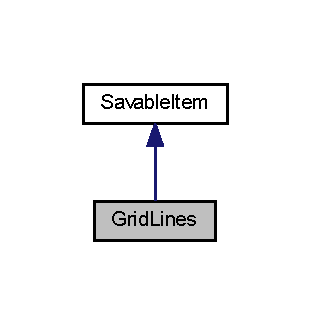
\includegraphics[width=149pt]{class_grid_lines__inherit__graph}
\end{center}
\end{figure}


Граф связей класса Grid\-Lines\-:
\nopagebreak
\begin{figure}[H]
\begin{center}
\leavevmode
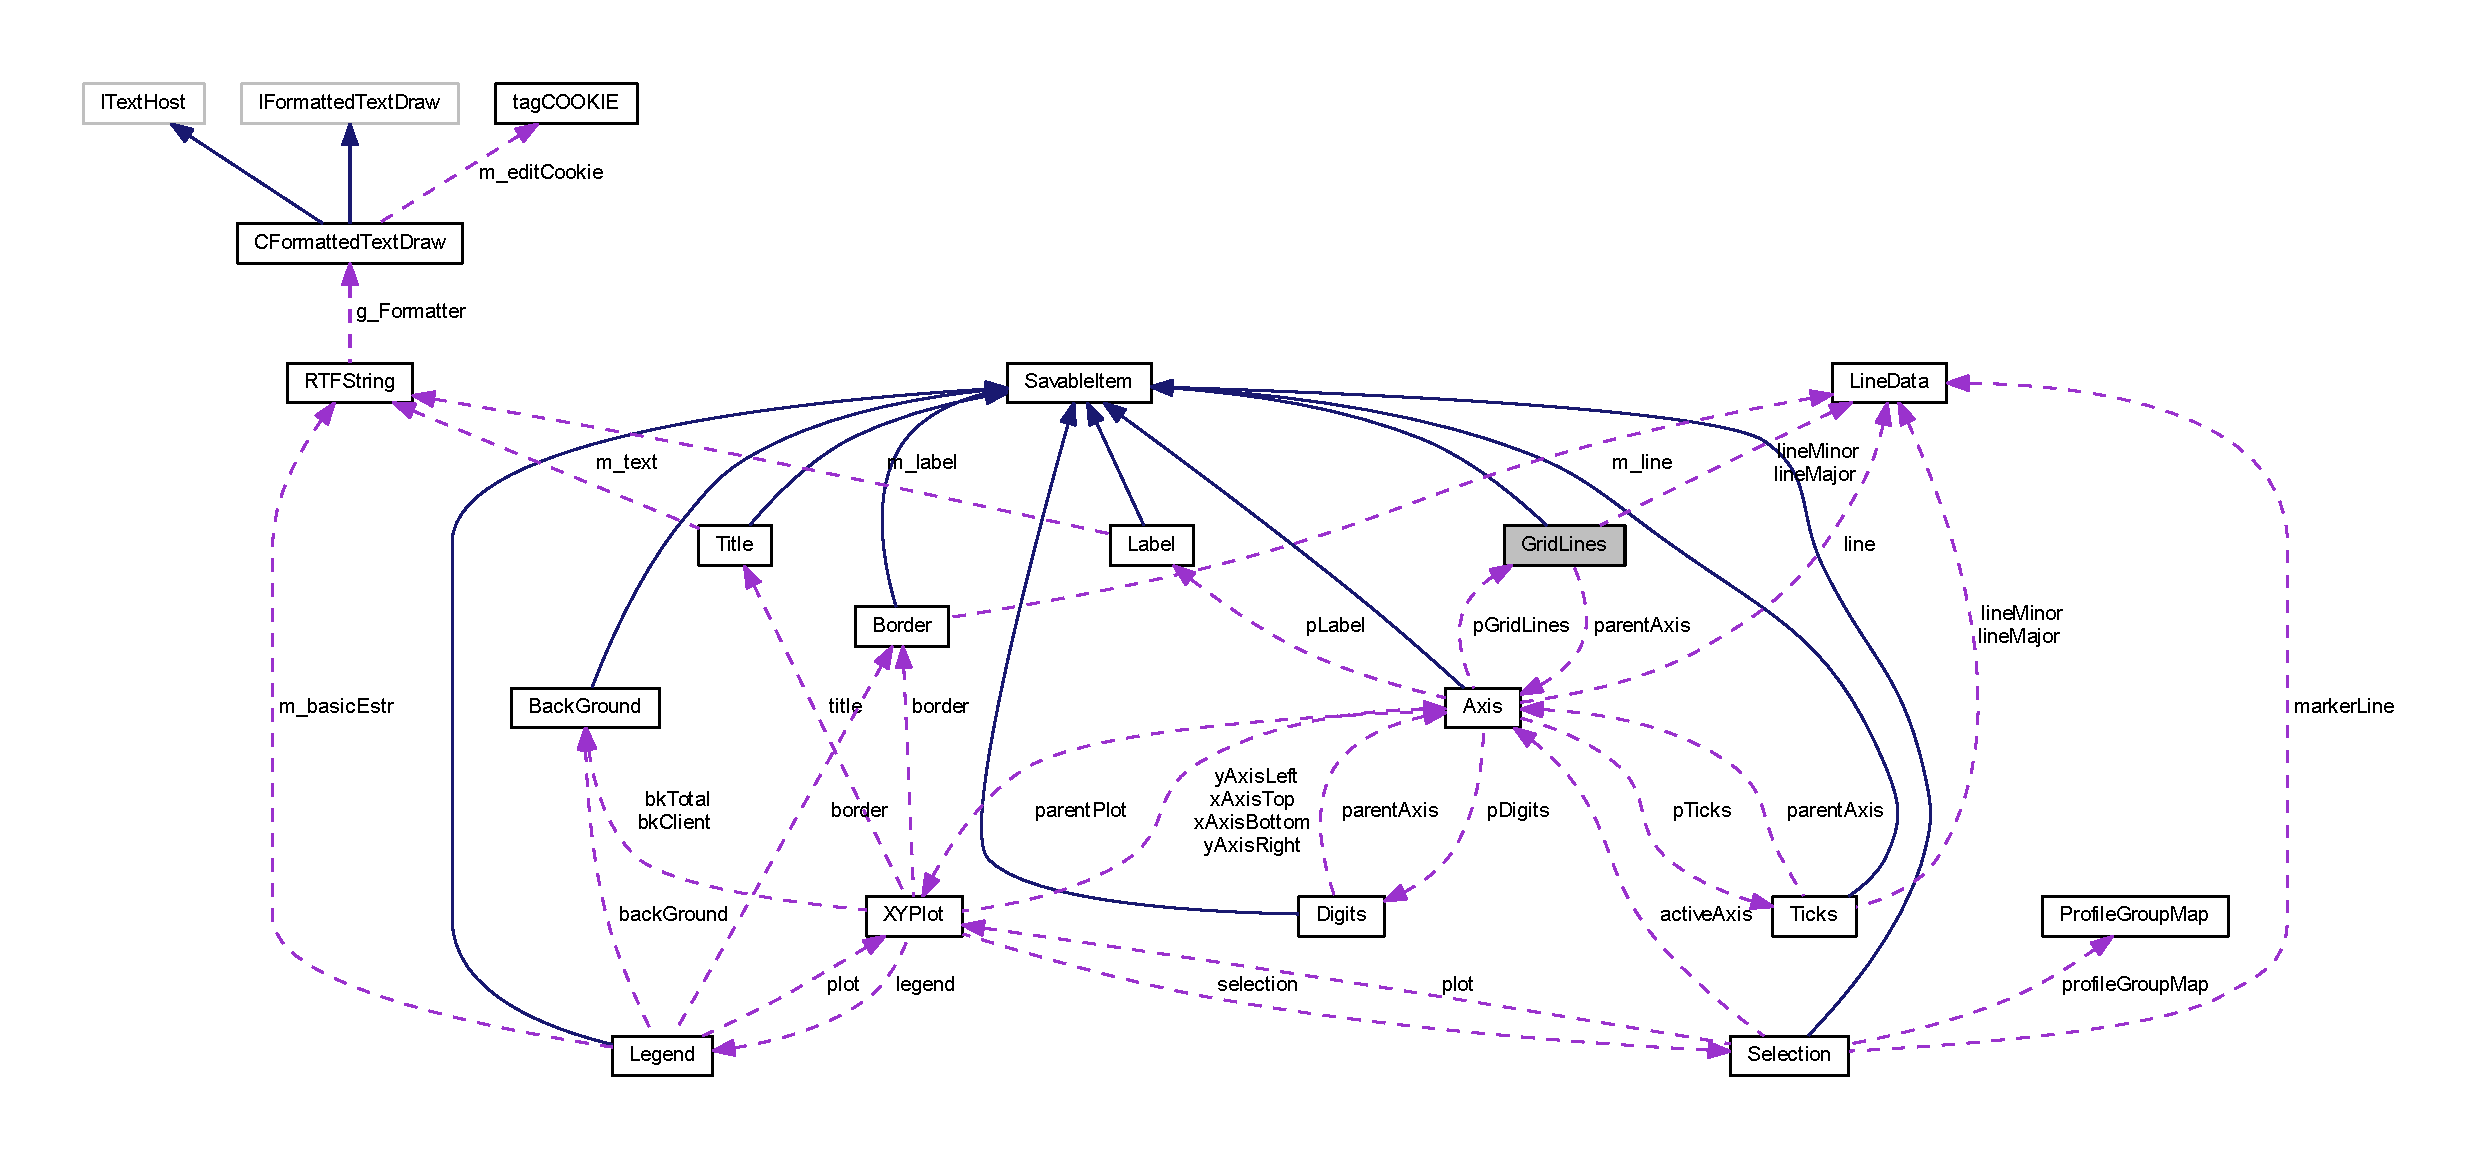
\includegraphics[width=350pt]{class_grid_lines__coll__graph}
\end{center}
\end{figure}
\subsection*{Открытые члены}
\begin{DoxyCompactItemize}
\item 
\hyperlink{class_grid_lines_a8b75ba08cc39e81740ccc456875f15f7}{Grid\-Lines} (\hyperlink{class_axis}{Axis} $\ast$\hyperlink{class_grid_lines_a1e3ebb07403f525c882731bb1662b234}{parent\-Axis})
\item 
virtual \hyperlink{class_grid_lines_afc1d1925713bf15c1f031d41a901016b}{$\sim$\-Grid\-Lines} ()
\item 
void \hyperlink{class_grid_lines_acefec88256cbb7dc4982e65666add9bb}{Enable\-Major} (B\-O\-O\-L enable=T\-R\-U\-E)
\item 
B\-O\-O\-L \hyperlink{class_grid_lines_a1208cfa5117f703ed785eba8c7ecae00}{Is\-Major\-Enabled} () const 
\item 
void \hyperlink{class_grid_lines_ab72907a0dcdb11acfeb473fb4c573939}{Enable\-Minor} (B\-O\-O\-L enable)
\item 
B\-O\-O\-L \hyperlink{class_grid_lines_af6a52af538900e6ec6cd6eb53ffa6d29}{Is\-Minor\-Enabled} () const 
\item 
\hyperlink{class_line_data}{Line\-Data} \& \hyperlink{class_grid_lines_a996a81d74b11f797745a3913b7c12293}{Get\-Line} (B\-O\-O\-L b\-Major=T\-R\-U\-E)
\item 
void \hyperlink{class_grid_lines_a420d336ed2892850bf5aab748d0fe406}{Set\-Line} (const \hyperlink{class_line_data}{Line\-Data} \&line, B\-O\-O\-L b\-Major=T\-R\-U\-E)
\item 
void \hyperlink{class_grid_lines_a839784fc12725e0705c751f8c9f466aa}{On\-Draw} (H\-D\-C hdc)
\item 
virtual B\-O\-O\-L \hyperlink{class_grid_lines_af41e725b2af5e093e5307e2096c2c4c7}{Write} (H\-A\-N\-D\-L\-E h\-File) const 
\item 
virtual B\-O\-O\-L \hyperlink{class_grid_lines_aecc543959e2bfa9c45345257433a3110}{Read} (H\-A\-N\-D\-L\-E h\-File)
\end{DoxyCompactItemize}
\subsection*{Защищенные данные}
\begin{DoxyCompactItemize}
\item 
\hyperlink{class_axis}{Axis} $\ast$ \hyperlink{class_grid_lines_a1e3ebb07403f525c882731bb1662b234}{parent\-Axis}
\item 
\hyperlink{class_line_data}{Line\-Data} $\ast$ \hyperlink{class_grid_lines_a3e368e27515f01143f5470b65c9f2a52}{line\-Major}
\item 
\hyperlink{class_line_data}{Line\-Data} $\ast$ \hyperlink{class_grid_lines_a72d2d255547ee192ff15609a254994fe}{line\-Minor}
\item 
B\-O\-O\-L \hyperlink{class_grid_lines_ad32092e3573f3fd24c3b1190f35034aa}{enabled\-Major}
\item 
B\-O\-O\-L \hyperlink{class_grid_lines_ae7f5d84d6a6b353e22fd251a20ac33f5}{enabled\-Minor}
\end{DoxyCompactItemize}
\subsection*{Дополнительные унаследованные члены}


\subsection{Конструктор(ы)}
\hypertarget{class_grid_lines_a8b75ba08cc39e81740ccc456875f15f7}{\index{Grid\-Lines@{Grid\-Lines}!Grid\-Lines@{Grid\-Lines}}
\index{Grid\-Lines@{Grid\-Lines}!GridLines@{Grid\-Lines}}
\subsubsection[{Grid\-Lines}]{\setlength{\rightskip}{0pt plus 5cm}Grid\-Lines\-::\-Grid\-Lines (
\begin{DoxyParamCaption}
\item[{{\bf Axis} $\ast$}]{parent\-Axis}
\end{DoxyParamCaption}
)}}\label{class_grid_lines_a8b75ba08cc39e81740ccc456875f15f7}
\hypertarget{class_grid_lines_afc1d1925713bf15c1f031d41a901016b}{\index{Grid\-Lines@{Grid\-Lines}!$\sim$\-Grid\-Lines@{$\sim$\-Grid\-Lines}}
\index{$\sim$\-Grid\-Lines@{$\sim$\-Grid\-Lines}!GridLines@{Grid\-Lines}}
\subsubsection[{$\sim$\-Grid\-Lines}]{\setlength{\rightskip}{0pt plus 5cm}Grid\-Lines\-::$\sim$\-Grid\-Lines (
\begin{DoxyParamCaption}
\item[{void}]{}
\end{DoxyParamCaption}
)\hspace{0.3cm}{\ttfamily [virtual]}}}\label{class_grid_lines_afc1d1925713bf15c1f031d41a901016b}


\subsection{Методы}
\hypertarget{class_grid_lines_acefec88256cbb7dc4982e65666add9bb}{\index{Grid\-Lines@{Grid\-Lines}!Enable\-Major@{Enable\-Major}}
\index{Enable\-Major@{Enable\-Major}!GridLines@{Grid\-Lines}}
\subsubsection[{Enable\-Major}]{\setlength{\rightskip}{0pt plus 5cm}void Grid\-Lines\-::\-Enable\-Major (
\begin{DoxyParamCaption}
\item[{B\-O\-O\-L}]{enable = {\ttfamily TRUE}}
\end{DoxyParamCaption}
)\hspace{0.3cm}{\ttfamily [inline]}}}\label{class_grid_lines_acefec88256cbb7dc4982e65666add9bb}
\hypertarget{class_grid_lines_ab72907a0dcdb11acfeb473fb4c573939}{\index{Grid\-Lines@{Grid\-Lines}!Enable\-Minor@{Enable\-Minor}}
\index{Enable\-Minor@{Enable\-Minor}!GridLines@{Grid\-Lines}}
\subsubsection[{Enable\-Minor}]{\setlength{\rightskip}{0pt plus 5cm}void Grid\-Lines\-::\-Enable\-Minor (
\begin{DoxyParamCaption}
\item[{B\-O\-O\-L}]{enable}
\end{DoxyParamCaption}
)\hspace{0.3cm}{\ttfamily [inline]}}}\label{class_grid_lines_ab72907a0dcdb11acfeb473fb4c573939}
\hypertarget{class_grid_lines_a996a81d74b11f797745a3913b7c12293}{\index{Grid\-Lines@{Grid\-Lines}!Get\-Line@{Get\-Line}}
\index{Get\-Line@{Get\-Line}!GridLines@{Grid\-Lines}}
\subsubsection[{Get\-Line}]{\setlength{\rightskip}{0pt plus 5cm}{\bf Line\-Data} \& Grid\-Lines\-::\-Get\-Line (
\begin{DoxyParamCaption}
\item[{B\-O\-O\-L}]{b\-Major = {\ttfamily TRUE}}
\end{DoxyParamCaption}
)}}\label{class_grid_lines_a996a81d74b11f797745a3913b7c12293}
\hypertarget{class_grid_lines_a1208cfa5117f703ed785eba8c7ecae00}{\index{Grid\-Lines@{Grid\-Lines}!Is\-Major\-Enabled@{Is\-Major\-Enabled}}
\index{Is\-Major\-Enabled@{Is\-Major\-Enabled}!GridLines@{Grid\-Lines}}
\subsubsection[{Is\-Major\-Enabled}]{\setlength{\rightskip}{0pt plus 5cm}B\-O\-O\-L Grid\-Lines\-::\-Is\-Major\-Enabled (
\begin{DoxyParamCaption}
{}
\end{DoxyParamCaption}
) const\hspace{0.3cm}{\ttfamily [inline]}}}\label{class_grid_lines_a1208cfa5117f703ed785eba8c7ecae00}
\hypertarget{class_grid_lines_af6a52af538900e6ec6cd6eb53ffa6d29}{\index{Grid\-Lines@{Grid\-Lines}!Is\-Minor\-Enabled@{Is\-Minor\-Enabled}}
\index{Is\-Minor\-Enabled@{Is\-Minor\-Enabled}!GridLines@{Grid\-Lines}}
\subsubsection[{Is\-Minor\-Enabled}]{\setlength{\rightskip}{0pt plus 5cm}B\-O\-O\-L Grid\-Lines\-::\-Is\-Minor\-Enabled (
\begin{DoxyParamCaption}
{}
\end{DoxyParamCaption}
) const\hspace{0.3cm}{\ttfamily [inline]}}}\label{class_grid_lines_af6a52af538900e6ec6cd6eb53ffa6d29}
\hypertarget{class_grid_lines_a839784fc12725e0705c751f8c9f466aa}{\index{Grid\-Lines@{Grid\-Lines}!On\-Draw@{On\-Draw}}
\index{On\-Draw@{On\-Draw}!GridLines@{Grid\-Lines}}
\subsubsection[{On\-Draw}]{\setlength{\rightskip}{0pt plus 5cm}void Grid\-Lines\-::\-On\-Draw (
\begin{DoxyParamCaption}
\item[{H\-D\-C}]{hdc}
\end{DoxyParamCaption}
)}}\label{class_grid_lines_a839784fc12725e0705c751f8c9f466aa}
\hypertarget{class_grid_lines_aecc543959e2bfa9c45345257433a3110}{\index{Grid\-Lines@{Grid\-Lines}!Read@{Read}}
\index{Read@{Read}!GridLines@{Grid\-Lines}}
\subsubsection[{Read}]{\setlength{\rightskip}{0pt plus 5cm}B\-O\-O\-L Grid\-Lines\-::\-Read (
\begin{DoxyParamCaption}
\item[{H\-A\-N\-D\-L\-E}]{h\-File}
\end{DoxyParamCaption}
)\hspace{0.3cm}{\ttfamily [virtual]}}}\label{class_grid_lines_aecc543959e2bfa9c45345257433a3110}


Замещает \hyperlink{class_savable_item_a7eadd16b2cb0652091cc15f596a00fb2}{Savable\-Item}.

\hypertarget{class_grid_lines_a420d336ed2892850bf5aab748d0fe406}{\index{Grid\-Lines@{Grid\-Lines}!Set\-Line@{Set\-Line}}
\index{Set\-Line@{Set\-Line}!GridLines@{Grid\-Lines}}
\subsubsection[{Set\-Line}]{\setlength{\rightskip}{0pt plus 5cm}void Grid\-Lines\-::\-Set\-Line (
\begin{DoxyParamCaption}
\item[{const {\bf Line\-Data} \&}]{line, }
\item[{B\-O\-O\-L}]{b\-Major = {\ttfamily TRUE}}
\end{DoxyParamCaption}
)}}\label{class_grid_lines_a420d336ed2892850bf5aab748d0fe406}
\hypertarget{class_grid_lines_af41e725b2af5e093e5307e2096c2c4c7}{\index{Grid\-Lines@{Grid\-Lines}!Write@{Write}}
\index{Write@{Write}!GridLines@{Grid\-Lines}}
\subsubsection[{Write}]{\setlength{\rightskip}{0pt plus 5cm}B\-O\-O\-L Grid\-Lines\-::\-Write (
\begin{DoxyParamCaption}
\item[{H\-A\-N\-D\-L\-E}]{h\-File}
\end{DoxyParamCaption}
) const\hspace{0.3cm}{\ttfamily [virtual]}}}\label{class_grid_lines_af41e725b2af5e093e5307e2096c2c4c7}


Замещает \hyperlink{class_savable_item_a0da511a4854f515096f8f9b498f64158}{Savable\-Item}.



\subsection{Данные класса}
\hypertarget{class_grid_lines_ad32092e3573f3fd24c3b1190f35034aa}{\index{Grid\-Lines@{Grid\-Lines}!enabled\-Major@{enabled\-Major}}
\index{enabled\-Major@{enabled\-Major}!GridLines@{Grid\-Lines}}
\subsubsection[{enabled\-Major}]{\setlength{\rightskip}{0pt plus 5cm}B\-O\-O\-L Grid\-Lines\-::enabled\-Major\hspace{0.3cm}{\ttfamily [protected]}}}\label{class_grid_lines_ad32092e3573f3fd24c3b1190f35034aa}
\hypertarget{class_grid_lines_ae7f5d84d6a6b353e22fd251a20ac33f5}{\index{Grid\-Lines@{Grid\-Lines}!enabled\-Minor@{enabled\-Minor}}
\index{enabled\-Minor@{enabled\-Minor}!GridLines@{Grid\-Lines}}
\subsubsection[{enabled\-Minor}]{\setlength{\rightskip}{0pt plus 5cm}B\-O\-O\-L Grid\-Lines\-::enabled\-Minor\hspace{0.3cm}{\ttfamily [protected]}}}\label{class_grid_lines_ae7f5d84d6a6b353e22fd251a20ac33f5}
\hypertarget{class_grid_lines_a3e368e27515f01143f5470b65c9f2a52}{\index{Grid\-Lines@{Grid\-Lines}!line\-Major@{line\-Major}}
\index{line\-Major@{line\-Major}!GridLines@{Grid\-Lines}}
\subsubsection[{line\-Major}]{\setlength{\rightskip}{0pt plus 5cm}{\bf Line\-Data}$\ast$ Grid\-Lines\-::line\-Major\hspace{0.3cm}{\ttfamily [protected]}}}\label{class_grid_lines_a3e368e27515f01143f5470b65c9f2a52}
\hypertarget{class_grid_lines_a72d2d255547ee192ff15609a254994fe}{\index{Grid\-Lines@{Grid\-Lines}!line\-Minor@{line\-Minor}}
\index{line\-Minor@{line\-Minor}!GridLines@{Grid\-Lines}}
\subsubsection[{line\-Minor}]{\setlength{\rightskip}{0pt plus 5cm}{\bf Line\-Data}$\ast$ Grid\-Lines\-::line\-Minor\hspace{0.3cm}{\ttfamily [protected]}}}\label{class_grid_lines_a72d2d255547ee192ff15609a254994fe}
\hypertarget{class_grid_lines_a1e3ebb07403f525c882731bb1662b234}{\index{Grid\-Lines@{Grid\-Lines}!parent\-Axis@{parent\-Axis}}
\index{parent\-Axis@{parent\-Axis}!GridLines@{Grid\-Lines}}
\subsubsection[{parent\-Axis}]{\setlength{\rightskip}{0pt plus 5cm}{\bf Axis}$\ast$ Grid\-Lines\-::parent\-Axis\hspace{0.3cm}{\ttfamily [protected]}}}\label{class_grid_lines_a1e3ebb07403f525c882731bb1662b234}


Объявления и описания членов классов находятся в файлах\-:\begin{DoxyCompactItemize}
\item 
src/\hyperlink{_gridlines_8h}{Gridlines.\-h}\item 
src/\hyperlink{_gridlines_8cpp}{Gridlines.\-cpp}\end{DoxyCompactItemize}

\hypertarget{classxyplot_1_1_h_g_r_o_u_p}{\section{Класс xyplot\-:\-:H\-G\-R\-O\-U\-P}
\label{classxyplot_1_1_h_g_r_o_u_p}\index{xyplot\-::\-H\-G\-R\-O\-U\-P@{xyplot\-::\-H\-G\-R\-O\-U\-P}}
}


Класс дескриптора группы профилей  




{\ttfamily \#include $<$X\-Y\-Plot\-Wrapper.\-h$>$}



Граф наследования\-:xyplot\-:\-:H\-G\-R\-O\-U\-P\-:\nopagebreak
\begin{figure}[H]
\begin{center}
\leavevmode
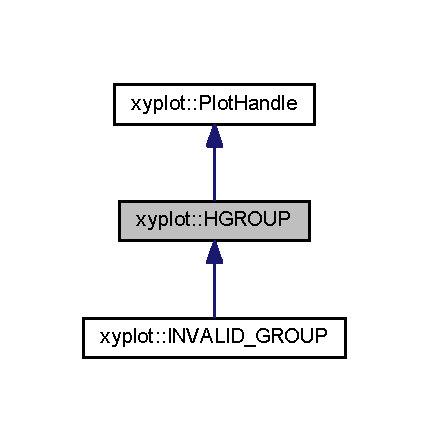
\includegraphics[width=206pt]{classxyplot_1_1_h_g_r_o_u_p__inherit__graph}
\end{center}
\end{figure}


Граф связей класса xyplot\-:\-:H\-G\-R\-O\-U\-P\-:\nopagebreak
\begin{figure}[H]
\begin{center}
\leavevmode
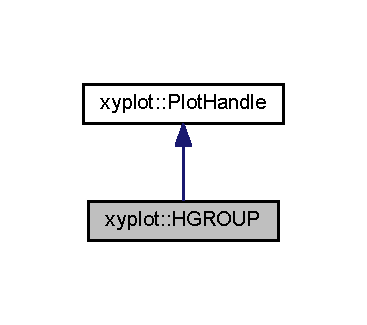
\includegraphics[width=176pt]{classxyplot_1_1_h_g_r_o_u_p__coll__graph}
\end{center}
\end{figure}
\subsection*{Открытые члены}
\begin{DoxyCompactItemize}
\item 
\hyperlink{classxyplot_1_1_h_g_r_o_u_p_a3606052deb19c27928d3b1db7b9d80f7}{H\-G\-R\-O\-U\-P} ()
\end{DoxyCompactItemize}
\subsection*{Защищенные члены}
\begin{DoxyCompactItemize}
\item 
\hyperlink{classxyplot_1_1_h_g_r_o_u_p_a51a309994a7bf3af80eb8da9d3275c37}{H\-G\-R\-O\-U\-P} (\hyperlink{namespacexyplot_a27bc71b0bdfac09495e7e531d8a918c5}{long} n)
\end{DoxyCompactItemize}
\subsection*{Друзья}
\begin{DoxyCompactItemize}
\item 
\hyperlink{classxyplot_1_1_h_g_r_o_u_p}{H\-G\-R\-O\-U\-P} \hyperlink{classxyplot_1_1_h_g_r_o_u_p_aad7a10078d1a6fe1f17b6c0e5511135a}{X\-Y\-Plot\-Manager\-::\-Create\-Group} (\hyperlink{classxyplot_1_1_h_p_l_o_t}{H\-P\-L\-O\-T} \&)
\end{DoxyCompactItemize}


\subsection{Подробное описание}
Класс дескриптора группы профилей 

\subsection{Конструктор(ы)}
\hypertarget{classxyplot_1_1_h_g_r_o_u_p_a3606052deb19c27928d3b1db7b9d80f7}{\index{xyplot\-::\-H\-G\-R\-O\-U\-P@{xyplot\-::\-H\-G\-R\-O\-U\-P}!H\-G\-R\-O\-U\-P@{H\-G\-R\-O\-U\-P}}
\index{H\-G\-R\-O\-U\-P@{H\-G\-R\-O\-U\-P}!xyplot::HGROUP@{xyplot\-::\-H\-G\-R\-O\-U\-P}}
\subsubsection[{H\-G\-R\-O\-U\-P}]{\setlength{\rightskip}{0pt plus 5cm}xyplot\-::\-H\-G\-R\-O\-U\-P\-::\-H\-G\-R\-O\-U\-P (
\begin{DoxyParamCaption}
{}
\end{DoxyParamCaption}
)\hspace{0.3cm}{\ttfamily [inline]}}}\label{classxyplot_1_1_h_g_r_o_u_p_a3606052deb19c27928d3b1db7b9d80f7}
\hypertarget{classxyplot_1_1_h_g_r_o_u_p_a51a309994a7bf3af80eb8da9d3275c37}{\index{xyplot\-::\-H\-G\-R\-O\-U\-P@{xyplot\-::\-H\-G\-R\-O\-U\-P}!H\-G\-R\-O\-U\-P@{H\-G\-R\-O\-U\-P}}
\index{H\-G\-R\-O\-U\-P@{H\-G\-R\-O\-U\-P}!xyplot::HGROUP@{xyplot\-::\-H\-G\-R\-O\-U\-P}}
\subsubsection[{H\-G\-R\-O\-U\-P}]{\setlength{\rightskip}{0pt plus 5cm}xyplot\-::\-H\-G\-R\-O\-U\-P\-::\-H\-G\-R\-O\-U\-P (
\begin{DoxyParamCaption}
\item[{{\bf long}}]{n}
\end{DoxyParamCaption}
)\hspace{0.3cm}{\ttfamily [inline]}, {\ttfamily [explicit]}, {\ttfamily [protected]}}}\label{classxyplot_1_1_h_g_r_o_u_p_a51a309994a7bf3af80eb8da9d3275c37}


\subsection{Документация по друзьям класса и функциям, отноносящимся к классу}
\hypertarget{classxyplot_1_1_h_g_r_o_u_p_aad7a10078d1a6fe1f17b6c0e5511135a}{\index{xyplot\-::\-H\-G\-R\-O\-U\-P@{xyplot\-::\-H\-G\-R\-O\-U\-P}!X\-Y\-Plot\-Manager\-::\-Create\-Group@{X\-Y\-Plot\-Manager\-::\-Create\-Group}}
\index{X\-Y\-Plot\-Manager\-::\-Create\-Group@{X\-Y\-Plot\-Manager\-::\-Create\-Group}!xyplot::HGROUP@{xyplot\-::\-H\-G\-R\-O\-U\-P}}
\subsubsection[{X\-Y\-Plot\-Manager\-::\-Create\-Group}]{\setlength{\rightskip}{0pt plus 5cm}{\bf H\-G\-R\-O\-U\-P} {\bf X\-Y\-Plot\-Manager\-::\-Create\-Group} (
\begin{DoxyParamCaption}
\item[{{\bf H\-P\-L\-O\-T} \&}]{}
\end{DoxyParamCaption}
)\hspace{0.3cm}{\ttfamily [friend]}}}\label{classxyplot_1_1_h_g_r_o_u_p_aad7a10078d1a6fe1f17b6c0e5511135a}


Объявления и описания членов класса находятся в файле\-:\begin{DoxyCompactItemize}
\item 
src/\hyperlink{_x_y_plot_wrapper_8h}{X\-Y\-Plot\-Wrapper.\-h}\end{DoxyCompactItemize}

\hypertarget{classxyplot_1_1_h_l_e_v_e_l}{\section{Класс xyplot\-:\-:H\-L\-E\-V\-E\-L}
\label{classxyplot_1_1_h_l_e_v_e_l}\index{xyplot\-::\-H\-L\-E\-V\-E\-L@{xyplot\-::\-H\-L\-E\-V\-E\-L}}
}


Класс дескриптор линий уровня  




{\ttfamily \#include $<$X\-Y\-Plot\-Wrapper.\-h$>$}



Граф наследования\-:xyplot\-:\-:H\-L\-E\-V\-E\-L\-:\nopagebreak
\begin{figure}[H]
\begin{center}
\leavevmode
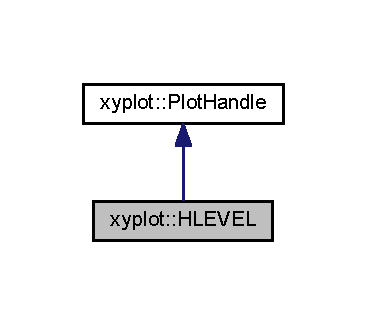
\includegraphics[width=176pt]{classxyplot_1_1_h_l_e_v_e_l__inherit__graph}
\end{center}
\end{figure}


Граф связей класса xyplot\-:\-:H\-L\-E\-V\-E\-L\-:\nopagebreak
\begin{figure}[H]
\begin{center}
\leavevmode
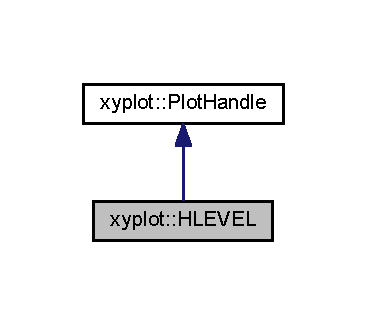
\includegraphics[width=176pt]{classxyplot_1_1_h_l_e_v_e_l__coll__graph}
\end{center}
\end{figure}
\subsection*{Открытые члены}
\begin{DoxyCompactItemize}
\item 
\hyperlink{classxyplot_1_1_h_l_e_v_e_l_adb83b057b07112c56e4ce303232c2b86}{H\-L\-E\-V\-E\-L} ()
\end{DoxyCompactItemize}
\subsection*{Защищенные члены}
\begin{DoxyCompactItemize}
\item 
\hyperlink{classxyplot_1_1_h_l_e_v_e_l_a575be341f182a5ace579b6ee079ae3fd}{H\-L\-E\-V\-E\-L} (\hyperlink{namespacexyplot_a27bc71b0bdfac09495e7e531d8a918c5}{long} n)
\end{DoxyCompactItemize}
\subsection*{Друзья}
\begin{DoxyCompactItemize}
\item 
\hyperlink{classxyplot_1_1_h_l_e_v_e_l}{H\-L\-E\-V\-E\-L} \hyperlink{classxyplot_1_1_h_l_e_v_e_l_af7f77d4596fc57ef8f51f4dba0fd1c97}{X\-Y\-Plot\-Manager\-::\-Create\-Level} (\hyperlink{classxyplot_1_1_h_p_l_o_t}{H\-P\-L\-O\-T} \&, \hyperlink{namespacexyplot_a27bc71b0bdfac09495e7e531d8a918c5}{long}, double, const char $\ast$, C\-O\-L\-O\-R\-R\-E\-F, int)
\end{DoxyCompactItemize}


\subsection{Подробное описание}
Класс дескриптор линий уровня 

\subsection{Конструктор(ы)}
\hypertarget{classxyplot_1_1_h_l_e_v_e_l_adb83b057b07112c56e4ce303232c2b86}{\index{xyplot\-::\-H\-L\-E\-V\-E\-L@{xyplot\-::\-H\-L\-E\-V\-E\-L}!H\-L\-E\-V\-E\-L@{H\-L\-E\-V\-E\-L}}
\index{H\-L\-E\-V\-E\-L@{H\-L\-E\-V\-E\-L}!xyplot::HLEVEL@{xyplot\-::\-H\-L\-E\-V\-E\-L}}
\subsubsection[{H\-L\-E\-V\-E\-L}]{\setlength{\rightskip}{0pt plus 5cm}xyplot\-::\-H\-L\-E\-V\-E\-L\-::\-H\-L\-E\-V\-E\-L (
\begin{DoxyParamCaption}
{}
\end{DoxyParamCaption}
)\hspace{0.3cm}{\ttfamily [inline]}}}\label{classxyplot_1_1_h_l_e_v_e_l_adb83b057b07112c56e4ce303232c2b86}
\hypertarget{classxyplot_1_1_h_l_e_v_e_l_a575be341f182a5ace579b6ee079ae3fd}{\index{xyplot\-::\-H\-L\-E\-V\-E\-L@{xyplot\-::\-H\-L\-E\-V\-E\-L}!H\-L\-E\-V\-E\-L@{H\-L\-E\-V\-E\-L}}
\index{H\-L\-E\-V\-E\-L@{H\-L\-E\-V\-E\-L}!xyplot::HLEVEL@{xyplot\-::\-H\-L\-E\-V\-E\-L}}
\subsubsection[{H\-L\-E\-V\-E\-L}]{\setlength{\rightskip}{0pt plus 5cm}xyplot\-::\-H\-L\-E\-V\-E\-L\-::\-H\-L\-E\-V\-E\-L (
\begin{DoxyParamCaption}
\item[{{\bf long}}]{n}
\end{DoxyParamCaption}
)\hspace{0.3cm}{\ttfamily [inline]}, {\ttfamily [explicit]}, {\ttfamily [protected]}}}\label{classxyplot_1_1_h_l_e_v_e_l_a575be341f182a5ace579b6ee079ae3fd}


\subsection{Документация по друзьям класса и функциям, отноносящимся к классу}
\hypertarget{classxyplot_1_1_h_l_e_v_e_l_af7f77d4596fc57ef8f51f4dba0fd1c97}{\index{xyplot\-::\-H\-L\-E\-V\-E\-L@{xyplot\-::\-H\-L\-E\-V\-E\-L}!X\-Y\-Plot\-Manager\-::\-Create\-Level@{X\-Y\-Plot\-Manager\-::\-Create\-Level}}
\index{X\-Y\-Plot\-Manager\-::\-Create\-Level@{X\-Y\-Plot\-Manager\-::\-Create\-Level}!xyplot::HLEVEL@{xyplot\-::\-H\-L\-E\-V\-E\-L}}
\subsubsection[{X\-Y\-Plot\-Manager\-::\-Create\-Level}]{\setlength{\rightskip}{0pt plus 5cm}{\bf H\-L\-E\-V\-E\-L} {\bf X\-Y\-Plot\-Manager\-::\-Create\-Level} (
\begin{DoxyParamCaption}
\item[{{\bf H\-P\-L\-O\-T} \&}]{, }
\item[{{\bf long}}]{, }
\item[{double}]{, }
\item[{const char $\ast$}]{, }
\item[{C\-O\-L\-O\-R\-R\-E\-F}]{, }
\item[{int}]{}
\end{DoxyParamCaption}
)\hspace{0.3cm}{\ttfamily [friend]}}}\label{classxyplot_1_1_h_l_e_v_e_l_af7f77d4596fc57ef8f51f4dba0fd1c97}


Объявления и описания членов класса находятся в файле\-:\begin{DoxyCompactItemize}
\item 
src/\hyperlink{_x_y_plot_wrapper_8h}{X\-Y\-Plot\-Wrapper.\-h}\end{DoxyCompactItemize}

\hypertarget{classxyplot_1_1_h_p_l_o_t}{\section{Класс xyplot\-:\-:H\-P\-L\-O\-T}
\label{classxyplot_1_1_h_p_l_o_t}\index{xyplot\-::\-H\-P\-L\-O\-T@{xyplot\-::\-H\-P\-L\-O\-T}}
}


Класс дескриптора 2\-D графики  




{\ttfamily \#include $<$X\-Y\-Plot\-Wrapper.\-h$>$}



Граф наследования\-:xyplot\-:\-:H\-P\-L\-O\-T\-:\nopagebreak
\begin{figure}[H]
\begin{center}
\leavevmode
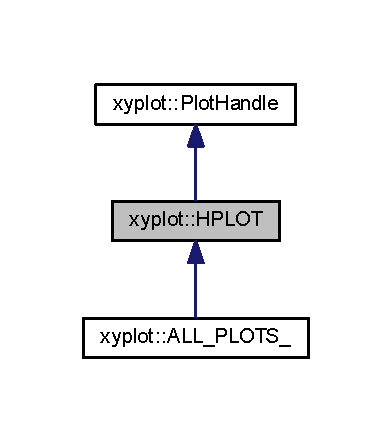
\includegraphics[width=188pt]{classxyplot_1_1_h_p_l_o_t__inherit__graph}
\end{center}
\end{figure}


Граф связей класса xyplot\-:\-:H\-P\-L\-O\-T\-:\nopagebreak
\begin{figure}[H]
\begin{center}
\leavevmode
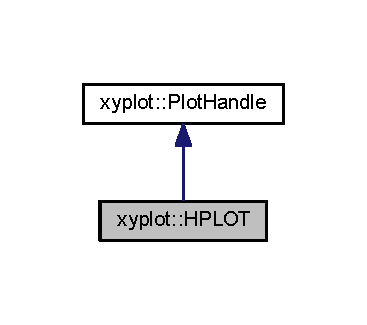
\includegraphics[width=176pt]{classxyplot_1_1_h_p_l_o_t__coll__graph}
\end{center}
\end{figure}
\subsection*{Открытые члены}
\begin{DoxyCompactItemize}
\item 
\hyperlink{classxyplot_1_1_h_p_l_o_t_a424db5c2119d13d2d3dbb002a0ac1a88}{H\-P\-L\-O\-T} ()
\end{DoxyCompactItemize}
\subsection*{Защищенные члены}
\begin{DoxyCompactItemize}
\item 
\hyperlink{classxyplot_1_1_h_p_l_o_t_a616541018b4726d067f5f0f603a7b728}{H\-P\-L\-O\-T} (\hyperlink{namespacexyplot_a27bc71b0bdfac09495e7e531d8a918c5}{long} n)
\end{DoxyCompactItemize}
\subsection*{Друзья}
\begin{DoxyCompactItemize}
\item 
\hyperlink{classxyplot_1_1_h_p_l_o_t}{H\-P\-L\-O\-T} \hyperlink{classxyplot_1_1_h_p_l_o_t_a2dc937508f64b152af97927dca16abfb}{X\-Y\-Plot\-Manager\-::\-Create\-Plot} (H\-W\-N\-D hwnd)
\end{DoxyCompactItemize}


\subsection{Подробное описание}
Класс дескриптора 2\-D графики 

\subsection{Конструктор(ы)}
\hypertarget{classxyplot_1_1_h_p_l_o_t_a424db5c2119d13d2d3dbb002a0ac1a88}{\index{xyplot\-::\-H\-P\-L\-O\-T@{xyplot\-::\-H\-P\-L\-O\-T}!H\-P\-L\-O\-T@{H\-P\-L\-O\-T}}
\index{H\-P\-L\-O\-T@{H\-P\-L\-O\-T}!xyplot::HPLOT@{xyplot\-::\-H\-P\-L\-O\-T}}
\subsubsection[{H\-P\-L\-O\-T}]{\setlength{\rightskip}{0pt plus 5cm}xyplot\-::\-H\-P\-L\-O\-T\-::\-H\-P\-L\-O\-T (
\begin{DoxyParamCaption}
{}
\end{DoxyParamCaption}
)\hspace{0.3cm}{\ttfamily [inline]}}}\label{classxyplot_1_1_h_p_l_o_t_a424db5c2119d13d2d3dbb002a0ac1a88}
Конструктор по умолчанию. Инициализирует пустой дескриптор (= 0) \hypertarget{classxyplot_1_1_h_p_l_o_t_a616541018b4726d067f5f0f603a7b728}{\index{xyplot\-::\-H\-P\-L\-O\-T@{xyplot\-::\-H\-P\-L\-O\-T}!H\-P\-L\-O\-T@{H\-P\-L\-O\-T}}
\index{H\-P\-L\-O\-T@{H\-P\-L\-O\-T}!xyplot::HPLOT@{xyplot\-::\-H\-P\-L\-O\-T}}
\subsubsection[{H\-P\-L\-O\-T}]{\setlength{\rightskip}{0pt plus 5cm}xyplot\-::\-H\-P\-L\-O\-T\-::\-H\-P\-L\-O\-T (
\begin{DoxyParamCaption}
\item[{{\bf long}}]{n}
\end{DoxyParamCaption}
)\hspace{0.3cm}{\ttfamily [inline]}, {\ttfamily [explicit]}, {\ttfamily [protected]}}}\label{classxyplot_1_1_h_p_l_o_t_a616541018b4726d067f5f0f603a7b728}
Конструктор с параметром. 
\begin{DoxyParams}{Аргументы}
{\em n} & -\/ ??? \\
\hline
\end{DoxyParams}


\subsection{Документация по друзьям класса и функциям, отноносящимся к классу}
\hypertarget{classxyplot_1_1_h_p_l_o_t_a2dc937508f64b152af97927dca16abfb}{\index{xyplot\-::\-H\-P\-L\-O\-T@{xyplot\-::\-H\-P\-L\-O\-T}!X\-Y\-Plot\-Manager\-::\-Create\-Plot@{X\-Y\-Plot\-Manager\-::\-Create\-Plot}}
\index{X\-Y\-Plot\-Manager\-::\-Create\-Plot@{X\-Y\-Plot\-Manager\-::\-Create\-Plot}!xyplot::HPLOT@{xyplot\-::\-H\-P\-L\-O\-T}}
\subsubsection[{X\-Y\-Plot\-Manager\-::\-Create\-Plot}]{\setlength{\rightskip}{0pt plus 5cm}{\bf H\-P\-L\-O\-T} {\bf X\-Y\-Plot\-Manager\-::\-Create\-Plot} (
\begin{DoxyParamCaption}
\item[{H\-W\-N\-D}]{hwnd}
\end{DoxyParamCaption}
)\hspace{0.3cm}{\ttfamily [friend]}}}\label{classxyplot_1_1_h_p_l_o_t_a2dc937508f64b152af97927dca16abfb}
Дружественная функция из класса \hyperlink{classxyplot_1_1_x_y_plot_manager}{X\-Y\-Plot\-Manager} 
\begin{DoxyParams}{Аргументы}
{\em hwnd} & дескриптор окна для которого создается экземпляр 2\-D графики \\
\hline
\end{DoxyParams}
\begin{DoxyReturn}{Возвращает}
дескриптор экземпляра 2\-D графики
\end{DoxyReturn}

\begin{DoxyCode}
XYPlotManager& pm = \hyperlink{classxyplot_1_1_x_y_plot_manager_abfde221555f11c692969986174781780}{XYPlotManager::Instance}();
\textcolor{keywordflow}{if} ( !pm.Initialize(\textcolor{stringliteral}{"xyplot.dll"}, ::AfxGetMainWnd()->m\_hWnd))
    \textcolor{keywordflow}{return} FALSE;
\hyperlink{classxyplot_1_1_h_p_l_o_t_a424db5c2119d13d2d3dbb002a0ac1a88}{HPLOT} plot;
CChildView* pView = ...;\textcolor{comment}{//получить дескриптор окна в котором будет отображаться графика }
\textcolor{keywordflow}{try} \{
        plot = pm.CreatePlot(pView->m\_hWnd)
    \}
 \textcolor{keywordflow}{catch} (XYPlotRequestFailure& e)
 \{
        \textcolor{keywordflow}{return} FALSE;
 \}
\end{DoxyCode}
 

Объявления и описания членов класса находятся в файле\-:\begin{DoxyCompactItemize}
\item 
src/\hyperlink{_x_y_plot_wrapper_8h}{X\-Y\-Plot\-Wrapper.\-h}\end{DoxyCompactItemize}

\hypertarget{classxyplot_1_1_h_p_l_o_t_r_e_g_i_o_n}{\section{Класс xyplot\-:\-:H\-P\-L\-O\-T\-R\-E\-G\-I\-O\-N}
\label{classxyplot_1_1_h_p_l_o_t_r_e_g_i_o_n}\index{xyplot\-::\-H\-P\-L\-O\-T\-R\-E\-G\-I\-O\-N@{xyplot\-::\-H\-P\-L\-O\-T\-R\-E\-G\-I\-O\-N}}
}


Класс дескриптора региона  




{\ttfamily \#include $<$X\-Y\-Plot\-Wrapper.\-h$>$}



Граф наследования\-:xyplot\-:\-:H\-P\-L\-O\-T\-R\-E\-G\-I\-O\-N\-:\nopagebreak
\begin{figure}[H]
\begin{center}
\leavevmode
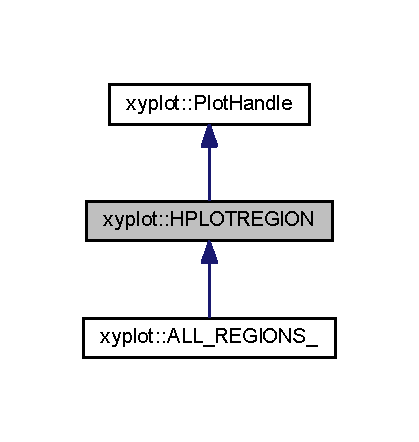
\includegraphics[width=201pt]{classxyplot_1_1_h_p_l_o_t_r_e_g_i_o_n__inherit__graph}
\end{center}
\end{figure}


Граф связей класса xyplot\-:\-:H\-P\-L\-O\-T\-R\-E\-G\-I\-O\-N\-:\nopagebreak
\begin{figure}[H]
\begin{center}
\leavevmode
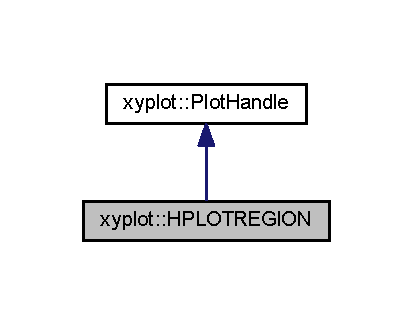
\includegraphics[width=198pt]{classxyplot_1_1_h_p_l_o_t_r_e_g_i_o_n__coll__graph}
\end{center}
\end{figure}
\subsection*{Открытые члены}
\begin{DoxyCompactItemize}
\item 
\hyperlink{classxyplot_1_1_h_p_l_o_t_r_e_g_i_o_n_a677cb699a43af8287c064a13c6da2657}{H\-P\-L\-O\-T\-R\-E\-G\-I\-O\-N} ()
\end{DoxyCompactItemize}
\subsection*{Защищенные члены}
\begin{DoxyCompactItemize}
\item 
\hyperlink{classxyplot_1_1_h_p_l_o_t_r_e_g_i_o_n_a78bccc9ad3433621e0447d0943a3583e}{H\-P\-L\-O\-T\-R\-E\-G\-I\-O\-N} (\hyperlink{namespacexyplot_a27bc71b0bdfac09495e7e531d8a918c5}{long} n)
\end{DoxyCompactItemize}
\subsection*{Друзья}
\begin{DoxyCompactItemize}
\item 
\hyperlink{classxyplot_1_1_h_p_l_o_t_r_e_g_i_o_n}{H\-P\-L\-O\-T\-R\-E\-G\-I\-O\-N} \hyperlink{classxyplot_1_1_h_p_l_o_t_r_e_g_i_o_n_afa1601e2b07b76f8076693c7f921e24f}{X\-Y\-Plot\-Manager\-::\-Create\-Region} (\hyperlink{classxyplot_1_1_h_p_l_o_t}{H\-P\-L\-O\-T} \&, \hyperlink{namespacexyplot_a27bc71b0bdfac09495e7e531d8a918c5}{long}, \hyperlink{namespacexyplot_a27bc71b0bdfac09495e7e531d8a918c5}{long}, double, double, double, double, const char $\ast$)
\end{DoxyCompactItemize}


\subsection{Подробное описание}
Класс дескриптора региона 

\subsection{Конструктор(ы)}
\hypertarget{classxyplot_1_1_h_p_l_o_t_r_e_g_i_o_n_a677cb699a43af8287c064a13c6da2657}{\index{xyplot\-::\-H\-P\-L\-O\-T\-R\-E\-G\-I\-O\-N@{xyplot\-::\-H\-P\-L\-O\-T\-R\-E\-G\-I\-O\-N}!H\-P\-L\-O\-T\-R\-E\-G\-I\-O\-N@{H\-P\-L\-O\-T\-R\-E\-G\-I\-O\-N}}
\index{H\-P\-L\-O\-T\-R\-E\-G\-I\-O\-N@{H\-P\-L\-O\-T\-R\-E\-G\-I\-O\-N}!xyplot::HPLOTREGION@{xyplot\-::\-H\-P\-L\-O\-T\-R\-E\-G\-I\-O\-N}}
\subsubsection[{H\-P\-L\-O\-T\-R\-E\-G\-I\-O\-N}]{\setlength{\rightskip}{0pt plus 5cm}xyplot\-::\-H\-P\-L\-O\-T\-R\-E\-G\-I\-O\-N\-::\-H\-P\-L\-O\-T\-R\-E\-G\-I\-O\-N (
\begin{DoxyParamCaption}
{}
\end{DoxyParamCaption}
)\hspace{0.3cm}{\ttfamily [inline]}}}\label{classxyplot_1_1_h_p_l_o_t_r_e_g_i_o_n_a677cb699a43af8287c064a13c6da2657}
\hypertarget{classxyplot_1_1_h_p_l_o_t_r_e_g_i_o_n_a78bccc9ad3433621e0447d0943a3583e}{\index{xyplot\-::\-H\-P\-L\-O\-T\-R\-E\-G\-I\-O\-N@{xyplot\-::\-H\-P\-L\-O\-T\-R\-E\-G\-I\-O\-N}!H\-P\-L\-O\-T\-R\-E\-G\-I\-O\-N@{H\-P\-L\-O\-T\-R\-E\-G\-I\-O\-N}}
\index{H\-P\-L\-O\-T\-R\-E\-G\-I\-O\-N@{H\-P\-L\-O\-T\-R\-E\-G\-I\-O\-N}!xyplot::HPLOTREGION@{xyplot\-::\-H\-P\-L\-O\-T\-R\-E\-G\-I\-O\-N}}
\subsubsection[{H\-P\-L\-O\-T\-R\-E\-G\-I\-O\-N}]{\setlength{\rightskip}{0pt plus 5cm}xyplot\-::\-H\-P\-L\-O\-T\-R\-E\-G\-I\-O\-N\-::\-H\-P\-L\-O\-T\-R\-E\-G\-I\-O\-N (
\begin{DoxyParamCaption}
\item[{{\bf long}}]{n}
\end{DoxyParamCaption}
)\hspace{0.3cm}{\ttfamily [inline]}, {\ttfamily [explicit]}, {\ttfamily [protected]}}}\label{classxyplot_1_1_h_p_l_o_t_r_e_g_i_o_n_a78bccc9ad3433621e0447d0943a3583e}


\subsection{Документация по друзьям класса и функциям, отноносящимся к классу}
\hypertarget{classxyplot_1_1_h_p_l_o_t_r_e_g_i_o_n_afa1601e2b07b76f8076693c7f921e24f}{\index{xyplot\-::\-H\-P\-L\-O\-T\-R\-E\-G\-I\-O\-N@{xyplot\-::\-H\-P\-L\-O\-T\-R\-E\-G\-I\-O\-N}!X\-Y\-Plot\-Manager\-::\-Create\-Region@{X\-Y\-Plot\-Manager\-::\-Create\-Region}}
\index{X\-Y\-Plot\-Manager\-::\-Create\-Region@{X\-Y\-Plot\-Manager\-::\-Create\-Region}!xyplot::HPLOTREGION@{xyplot\-::\-H\-P\-L\-O\-T\-R\-E\-G\-I\-O\-N}}
\subsubsection[{X\-Y\-Plot\-Manager\-::\-Create\-Region}]{\setlength{\rightskip}{0pt plus 5cm}{\bf H\-P\-L\-O\-T\-R\-E\-G\-I\-O\-N} {\bf X\-Y\-Plot\-Manager\-::\-Create\-Region} (
\begin{DoxyParamCaption}
\item[{{\bf H\-P\-L\-O\-T} \&}]{, }
\item[{{\bf long}}]{, }
\item[{{\bf long}}]{, }
\item[{double}]{, }
\item[{double}]{, }
\item[{double}]{, }
\item[{double}]{, }
\item[{const char $\ast$}]{}
\end{DoxyParamCaption}
)\hspace{0.3cm}{\ttfamily [friend]}}}\label{classxyplot_1_1_h_p_l_o_t_r_e_g_i_o_n_afa1601e2b07b76f8076693c7f921e24f}


Объявления и описания членов класса находятся в файле\-:\begin{DoxyCompactItemize}
\item 
src/\hyperlink{_x_y_plot_wrapper_8h}{X\-Y\-Plot\-Wrapper.\-h}\end{DoxyCompactItemize}

\hypertarget{classxyplot_1_1_h_p_r_o_f_i_l_e}{\section{Класс xyplot\-:\-:H\-P\-R\-O\-F\-I\-L\-E}
\label{classxyplot_1_1_h_p_r_o_f_i_l_e}\index{xyplot\-::\-H\-P\-R\-O\-F\-I\-L\-E@{xyplot\-::\-H\-P\-R\-O\-F\-I\-L\-E}}
}


Класс дескриптора профиля  




{\ttfamily \#include $<$X\-Y\-Plot\-Wrapper.\-h$>$}



Граф наследования\-:xyplot\-:\-:H\-P\-R\-O\-F\-I\-L\-E\-:\nopagebreak
\begin{figure}[H]
\begin{center}
\leavevmode
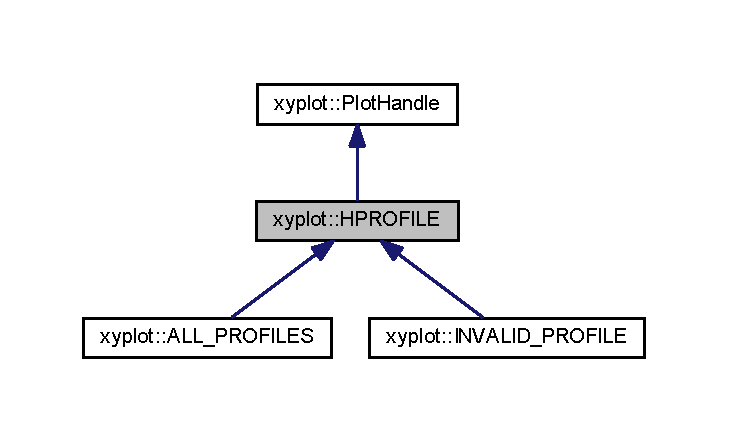
\includegraphics[width=350pt]{classxyplot_1_1_h_p_r_o_f_i_l_e__inherit__graph}
\end{center}
\end{figure}


Граф связей класса xyplot\-:\-:H\-P\-R\-O\-F\-I\-L\-E\-:\nopagebreak
\begin{figure}[H]
\begin{center}
\leavevmode
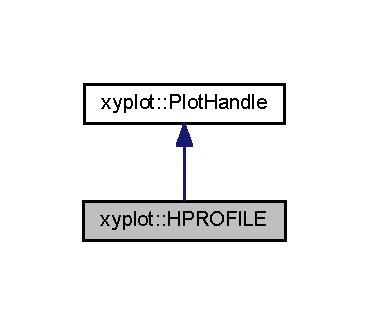
\includegraphics[width=177pt]{classxyplot_1_1_h_p_r_o_f_i_l_e__coll__graph}
\end{center}
\end{figure}
\subsection*{Открытые члены}
\begin{DoxyCompactItemize}
\item 
\hyperlink{classxyplot_1_1_h_p_r_o_f_i_l_e_a70804411bb38e9b9c7304dc71335c823}{H\-P\-R\-O\-F\-I\-L\-E} ()
\end{DoxyCompactItemize}
\subsection*{Защищенные члены}
\begin{DoxyCompactItemize}
\item 
\hyperlink{classxyplot_1_1_h_p_r_o_f_i_l_e_a179d13e5b95a14c9188d3c6f6654d4ae}{H\-P\-R\-O\-F\-I\-L\-E} (\hyperlink{namespacexyplot_a27bc71b0bdfac09495e7e531d8a918c5}{long} n)
\end{DoxyCompactItemize}
\subsection*{Друзья}
\begin{DoxyCompactItemize}
\item 
\hyperlink{classxyplot_1_1_h_p_r_o_f_i_l_e}{H\-P\-R\-O\-F\-I\-L\-E} \hyperlink{classxyplot_1_1_h_p_r_o_f_i_l_e_a6850dbfafb6d482146f5a6da4a7d62ec}{X\-Y\-Plot\-Manager\-::\-Create\-Profile} (\hyperlink{classxyplot_1_1_h_p_l_o_t}{H\-P\-L\-O\-T} \&h\-Plot, const char $\ast$name, C\-O\-L\-O\-R\-R\-E\-F color, int width, int line\-Type, const char $\ast$sz\-Line\-Template, B\-O\-O\-L visible, B\-O\-O\-L showmarks, \hyperlink{namespacexyplot_a27bc71b0bdfac09495e7e531d8a918c5}{long} x\-Parent\-Axis, \hyperlink{namespacexyplot_a27bc71b0bdfac09495e7e531d8a918c5}{long} y\-Parent\-Axis)
\item 
B\-O\-O\-L \hyperlink{classxyplot_1_1_h_p_r_o_f_i_l_e_a899707577b96da846fcf3489bd3e483b}{X\-Y\-Plot\-Manager\-::\-Get\-Profile\-List} (\hyperlink{classxyplot_1_1_h_p_l_o_t}{H\-P\-L\-O\-T} \&, std\-::vector$<$ \hyperlink{classxyplot_1_1_h_p_r_o_f_i_l_e}{H\-P\-R\-O\-F\-I\-L\-E} $>$ \&)
\end{DoxyCompactItemize}


\subsection{Подробное описание}
Класс дескриптора профиля 

\subsection{Конструктор(ы)}
\hypertarget{classxyplot_1_1_h_p_r_o_f_i_l_e_a70804411bb38e9b9c7304dc71335c823}{\index{xyplot\-::\-H\-P\-R\-O\-F\-I\-L\-E@{xyplot\-::\-H\-P\-R\-O\-F\-I\-L\-E}!H\-P\-R\-O\-F\-I\-L\-E@{H\-P\-R\-O\-F\-I\-L\-E}}
\index{H\-P\-R\-O\-F\-I\-L\-E@{H\-P\-R\-O\-F\-I\-L\-E}!xyplot::HPROFILE@{xyplot\-::\-H\-P\-R\-O\-F\-I\-L\-E}}
\subsubsection[{H\-P\-R\-O\-F\-I\-L\-E}]{\setlength{\rightskip}{0pt plus 5cm}xyplot\-::\-H\-P\-R\-O\-F\-I\-L\-E\-::\-H\-P\-R\-O\-F\-I\-L\-E (
\begin{DoxyParamCaption}
{}
\end{DoxyParamCaption}
)\hspace{0.3cm}{\ttfamily [inline]}}}\label{classxyplot_1_1_h_p_r_o_f_i_l_e_a70804411bb38e9b9c7304dc71335c823}
Конструктор по умолчанию. \hypertarget{classxyplot_1_1_h_p_r_o_f_i_l_e_a179d13e5b95a14c9188d3c6f6654d4ae}{\index{xyplot\-::\-H\-P\-R\-O\-F\-I\-L\-E@{xyplot\-::\-H\-P\-R\-O\-F\-I\-L\-E}!H\-P\-R\-O\-F\-I\-L\-E@{H\-P\-R\-O\-F\-I\-L\-E}}
\index{H\-P\-R\-O\-F\-I\-L\-E@{H\-P\-R\-O\-F\-I\-L\-E}!xyplot::HPROFILE@{xyplot\-::\-H\-P\-R\-O\-F\-I\-L\-E}}
\subsubsection[{H\-P\-R\-O\-F\-I\-L\-E}]{\setlength{\rightskip}{0pt plus 5cm}xyplot\-::\-H\-P\-R\-O\-F\-I\-L\-E\-::\-H\-P\-R\-O\-F\-I\-L\-E (
\begin{DoxyParamCaption}
\item[{{\bf long}}]{n}
\end{DoxyParamCaption}
)\hspace{0.3cm}{\ttfamily [inline]}, {\ttfamily [explicit]}, {\ttfamily [protected]}}}\label{classxyplot_1_1_h_p_r_o_f_i_l_e_a179d13e5b95a14c9188d3c6f6654d4ae}


\subsection{Документация по друзьям класса и функциям, отноносящимся к классу}
\hypertarget{classxyplot_1_1_h_p_r_o_f_i_l_e_a6850dbfafb6d482146f5a6da4a7d62ec}{\index{xyplot\-::\-H\-P\-R\-O\-F\-I\-L\-E@{xyplot\-::\-H\-P\-R\-O\-F\-I\-L\-E}!X\-Y\-Plot\-Manager\-::\-Create\-Profile@{X\-Y\-Plot\-Manager\-::\-Create\-Profile}}
\index{X\-Y\-Plot\-Manager\-::\-Create\-Profile@{X\-Y\-Plot\-Manager\-::\-Create\-Profile}!xyplot::HPROFILE@{xyplot\-::\-H\-P\-R\-O\-F\-I\-L\-E}}
\subsubsection[{X\-Y\-Plot\-Manager\-::\-Create\-Profile}]{\setlength{\rightskip}{0pt plus 5cm}{\bf H\-P\-R\-O\-F\-I\-L\-E} {\bf X\-Y\-Plot\-Manager\-::\-Create\-Profile} (
\begin{DoxyParamCaption}
\item[{{\bf H\-P\-L\-O\-T} \&}]{h\-Plot, }
\item[{const char $\ast$}]{name, }
\item[{C\-O\-L\-O\-R\-R\-E\-F}]{color, }
\item[{int}]{width, }
\item[{int}]{line\-Type, }
\item[{const char $\ast$}]{sz\-Line\-Template, }
\item[{B\-O\-O\-L}]{visible, }
\item[{B\-O\-O\-L}]{showmarks, }
\item[{{\bf long}}]{x\-Parent\-Axis, }
\item[{{\bf long}}]{y\-Parent\-Axis}
\end{DoxyParamCaption}
)\hspace{0.3cm}{\ttfamily [friend]}}}\label{classxyplot_1_1_h_p_r_o_f_i_l_e_a6850dbfafb6d482146f5a6da4a7d62ec}
Дружественная функция из класса \hyperlink{classxyplot_1_1_x_y_plot_manager}{X\-Y\-Plot\-Manager} для создания экземпляра профиля 
\begin{DoxyParams}[1]{Аргументы}
\mbox{\tt in}  & {\em h\-Plot} & дескриптор экземпляра 2\-D графика для которого создается профиль \\
\hline
 & {\em name} & имя профиля (отображается в легенде) \\
\hline
 & {\em color} & цвет профиля \\
\hline
 & {\em width} & толщина линии профиля в пикселях \\
\hline
 & {\em line\-Type} & тип линии профиля \begin{DoxyItemize}
\item P\-L\-S\-\_\-\-I\-N\-V\-I\-S\-I\-B\-L\-E -\/ невидимая \item P\-L\-S\-\_\-\-S\-O\-L\-I\-D -\/ сплошная \item P\-L\-S\-\_\-\-D\-A\-S\-H -\/ штриховая \item P\-L\-S\-\_\-\-D\-O\-T -\/ точечная \item P\-L\-S\-\_\-\-D\-A\-S\-H\-D\-O\-T -\/ осевая \item P\-L\-S\-\_\-\-D\-A\-S\-H\-D\-O\-T\-D\-O\-T -\/ штрих-\/точка-\/точка \item P\-L\-S\-\_\-\-C\-U\-S\-T\-O\-M -\/ пользовательсякая \end{DoxyItemize}
\\
\hline
 & {\em sz\-Line\-Template} & пользовательский шаблон линии. Данный аргумент используется только в случае если выбран пользовательский тип линии. Шаблон представляет собой последовательность целочисленных значений для задания интервалов заполнения и промежутков в пикселях. Например значение шаблона \char`\"{}5 2\char`\"{} означает, что 5px отрисовываются сплошной линией затем следует промежуток 2px. \\
\hline
 & {\em visible} & будет ли отображаться линия данного профиля \\
\hline
 & {\em showmarks} & отображать ли метки данных профиля \\
\hline
 & {\em x\-Parent\-Axis} & ось X, к которой прикрепляется профиль \\
\hline
 & {\em y\-Parent\-Axis} & ось Y, к которой прикрепляется профиль \\
\hline
\end{DoxyParams}
\begin{DoxyReturn}{Возвращает}
дескриптор экземпляра профиля
\end{DoxyReturn}

\begin{DoxyCode}
XYPlotManager& pm = \hyperlink{classxyplot_1_1_x_y_plot_manager_abfde221555f11c692969986174781780}{XYPlotManager::Instance}();
\textcolor{keywordflow}{if} ( !pm.Initialize(\textcolor{stringliteral}{"xyplot.dll"}, ::AfxGetMainWnd()->m\_hWnd))
    \textcolor{keywordflow}{return} FALSE;
HPLOT plot;
CChildView* pView = ...;\textcolor{comment}{//получить дескриптор окна в котором будет отображаться графика }
\textcolor{keywordflow}{try} \{
        plot = pm.CreatePlot(pView->m\_hWnd)
    \}
 \textcolor{keywordflow}{catch} (XYPlotRequestFailure& e)
 \{
        \textcolor{keywordflow}{return} FALSE;
 \}
\end{DoxyCode}
 \hypertarget{classxyplot_1_1_h_p_r_o_f_i_l_e_a899707577b96da846fcf3489bd3e483b}{\index{xyplot\-::\-H\-P\-R\-O\-F\-I\-L\-E@{xyplot\-::\-H\-P\-R\-O\-F\-I\-L\-E}!X\-Y\-Plot\-Manager\-::\-Get\-Profile\-List@{X\-Y\-Plot\-Manager\-::\-Get\-Profile\-List}}
\index{X\-Y\-Plot\-Manager\-::\-Get\-Profile\-List@{X\-Y\-Plot\-Manager\-::\-Get\-Profile\-List}!xyplot::HPROFILE@{xyplot\-::\-H\-P\-R\-O\-F\-I\-L\-E}}
\subsubsection[{X\-Y\-Plot\-Manager\-::\-Get\-Profile\-List}]{\setlength{\rightskip}{0pt plus 5cm}B\-O\-O\-L {\bf X\-Y\-Plot\-Manager\-::\-Get\-Profile\-List} (
\begin{DoxyParamCaption}
\item[{{\bf H\-P\-L\-O\-T} \&}]{, }
\item[{std\-::vector$<$ {\bf H\-P\-R\-O\-F\-I\-L\-E} $>$ \&}]{}
\end{DoxyParamCaption}
)\hspace{0.3cm}{\ttfamily [friend]}}}\label{classxyplot_1_1_h_p_r_o_f_i_l_e_a899707577b96da846fcf3489bd3e483b}


Объявления и описания членов класса находятся в файле\-:\begin{DoxyCompactItemize}
\item 
src/\hyperlink{_x_y_plot_wrapper_8h}{X\-Y\-Plot\-Wrapper.\-h}\end{DoxyCompactItemize}

\hypertarget{classxyplot_1_1_i_n_v_a_l_i_d___g_r_o_u_p}{\section{Класс xyplot\-:\-:I\-N\-V\-A\-L\-I\-D\-\_\-\-G\-R\-O\-U\-P}
\label{classxyplot_1_1_i_n_v_a_l_i_d___g_r_o_u_p}\index{xyplot\-::\-I\-N\-V\-A\-L\-I\-D\-\_\-\-G\-R\-O\-U\-P@{xyplot\-::\-I\-N\-V\-A\-L\-I\-D\-\_\-\-G\-R\-O\-U\-P}}
}


Класс дескриптор пустой группы профилей 2\-D графики  




{\ttfamily \#include $<$X\-Y\-Plot\-Wrapper.\-h$>$}



Граф наследования\-:xyplot\-:\-:I\-N\-V\-A\-L\-I\-D\-\_\-\-G\-R\-O\-U\-P\-:\nopagebreak
\begin{figure}[H]
\begin{center}
\leavevmode
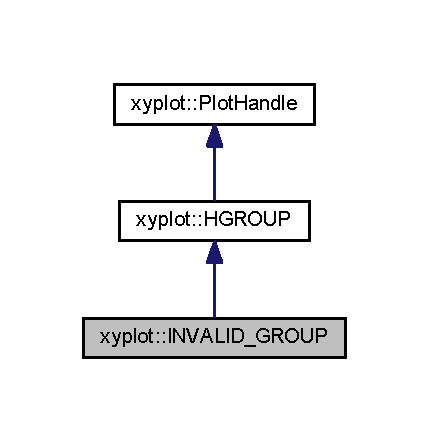
\includegraphics[width=206pt]{classxyplot_1_1_i_n_v_a_l_i_d___g_r_o_u_p__inherit__graph}
\end{center}
\end{figure}


Граф связей класса xyplot\-:\-:I\-N\-V\-A\-L\-I\-D\-\_\-\-G\-R\-O\-U\-P\-:\nopagebreak
\begin{figure}[H]
\begin{center}
\leavevmode
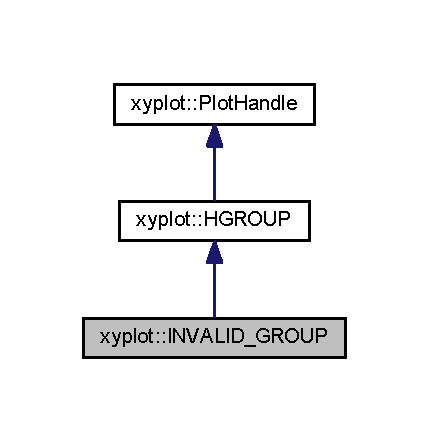
\includegraphics[width=206pt]{classxyplot_1_1_i_n_v_a_l_i_d___g_r_o_u_p__coll__graph}
\end{center}
\end{figure}
\subsection*{Открытые члены}
\begin{DoxyCompactItemize}
\item 
\hyperlink{classxyplot_1_1_i_n_v_a_l_i_d___g_r_o_u_p_a99387abde12e38431ad287cab789ce7e}{I\-N\-V\-A\-L\-I\-D\-\_\-\-G\-R\-O\-U\-P} ()
\end{DoxyCompactItemize}
\subsection*{Дополнительные унаследованные члены}


\subsection{Подробное описание}
Класс дескриптор пустой группы профилей 2\-D графики 

\subsection{Конструктор(ы)}
\hypertarget{classxyplot_1_1_i_n_v_a_l_i_d___g_r_o_u_p_a99387abde12e38431ad287cab789ce7e}{\index{xyplot\-::\-I\-N\-V\-A\-L\-I\-D\-\_\-\-G\-R\-O\-U\-P@{xyplot\-::\-I\-N\-V\-A\-L\-I\-D\-\_\-\-G\-R\-O\-U\-P}!I\-N\-V\-A\-L\-I\-D\-\_\-\-G\-R\-O\-U\-P@{I\-N\-V\-A\-L\-I\-D\-\_\-\-G\-R\-O\-U\-P}}
\index{I\-N\-V\-A\-L\-I\-D\-\_\-\-G\-R\-O\-U\-P@{I\-N\-V\-A\-L\-I\-D\-\_\-\-G\-R\-O\-U\-P}!xyplot::INVALID_GROUP@{xyplot\-::\-I\-N\-V\-A\-L\-I\-D\-\_\-\-G\-R\-O\-U\-P}}
\subsubsection[{I\-N\-V\-A\-L\-I\-D\-\_\-\-G\-R\-O\-U\-P}]{\setlength{\rightskip}{0pt plus 5cm}xyplot\-::\-I\-N\-V\-A\-L\-I\-D\-\_\-\-G\-R\-O\-U\-P\-::\-I\-N\-V\-A\-L\-I\-D\-\_\-\-G\-R\-O\-U\-P (
\begin{DoxyParamCaption}
{}
\end{DoxyParamCaption}
)\hspace{0.3cm}{\ttfamily [inline]}}}\label{classxyplot_1_1_i_n_v_a_l_i_d___g_r_o_u_p_a99387abde12e38431ad287cab789ce7e}


Объявления и описания членов класса находятся в файле\-:\begin{DoxyCompactItemize}
\item 
src/\hyperlink{_x_y_plot_wrapper_8h}{X\-Y\-Plot\-Wrapper.\-h}\end{DoxyCompactItemize}

\hypertarget{classxyplot_1_1_i_n_v_a_l_i_d___p_r_o_f_i_l_e}{\section{Класс xyplot\-:\-:I\-N\-V\-A\-L\-I\-D\-\_\-\-P\-R\-O\-F\-I\-L\-E}
\label{classxyplot_1_1_i_n_v_a_l_i_d___p_r_o_f_i_l_e}\index{xyplot\-::\-I\-N\-V\-A\-L\-I\-D\-\_\-\-P\-R\-O\-F\-I\-L\-E@{xyplot\-::\-I\-N\-V\-A\-L\-I\-D\-\_\-\-P\-R\-O\-F\-I\-L\-E}}
}


Класс дескриптор пустого профиля 2\-D графики  




{\ttfamily \#include $<$X\-Y\-Plot\-Wrapper.\-h$>$}



Граф наследования\-:xyplot\-:\-:I\-N\-V\-A\-L\-I\-D\-\_\-\-P\-R\-O\-F\-I\-L\-E\-:\nopagebreak
\begin{figure}[H]
\begin{center}
\leavevmode
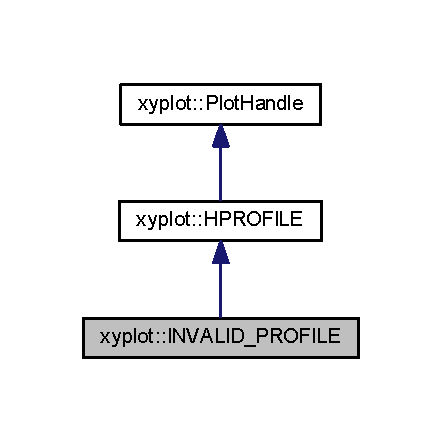
\includegraphics[width=212pt]{classxyplot_1_1_i_n_v_a_l_i_d___p_r_o_f_i_l_e__inherit__graph}
\end{center}
\end{figure}


Граф связей класса xyplot\-:\-:I\-N\-V\-A\-L\-I\-D\-\_\-\-P\-R\-O\-F\-I\-L\-E\-:\nopagebreak
\begin{figure}[H]
\begin{center}
\leavevmode
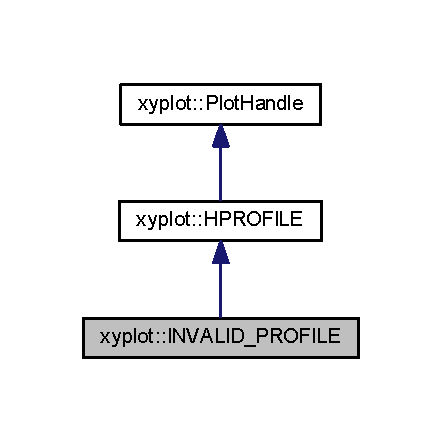
\includegraphics[width=212pt]{classxyplot_1_1_i_n_v_a_l_i_d___p_r_o_f_i_l_e__coll__graph}
\end{center}
\end{figure}
\subsection*{Открытые члены}
\begin{DoxyCompactItemize}
\item 
\hyperlink{classxyplot_1_1_i_n_v_a_l_i_d___p_r_o_f_i_l_e_a679ca1b1d0531ee7ccbd6cfb21f91932}{I\-N\-V\-A\-L\-I\-D\-\_\-\-P\-R\-O\-F\-I\-L\-E} ()
\end{DoxyCompactItemize}
\subsection*{Дополнительные унаследованные члены}


\subsection{Подробное описание}
Класс дескриптор пустого профиля 2\-D графики 

\subsection{Конструктор(ы)}
\hypertarget{classxyplot_1_1_i_n_v_a_l_i_d___p_r_o_f_i_l_e_a679ca1b1d0531ee7ccbd6cfb21f91932}{\index{xyplot\-::\-I\-N\-V\-A\-L\-I\-D\-\_\-\-P\-R\-O\-F\-I\-L\-E@{xyplot\-::\-I\-N\-V\-A\-L\-I\-D\-\_\-\-P\-R\-O\-F\-I\-L\-E}!I\-N\-V\-A\-L\-I\-D\-\_\-\-P\-R\-O\-F\-I\-L\-E@{I\-N\-V\-A\-L\-I\-D\-\_\-\-P\-R\-O\-F\-I\-L\-E}}
\index{I\-N\-V\-A\-L\-I\-D\-\_\-\-P\-R\-O\-F\-I\-L\-E@{I\-N\-V\-A\-L\-I\-D\-\_\-\-P\-R\-O\-F\-I\-L\-E}!xyplot::INVALID_PROFILE@{xyplot\-::\-I\-N\-V\-A\-L\-I\-D\-\_\-\-P\-R\-O\-F\-I\-L\-E}}
\subsubsection[{I\-N\-V\-A\-L\-I\-D\-\_\-\-P\-R\-O\-F\-I\-L\-E}]{\setlength{\rightskip}{0pt plus 5cm}xyplot\-::\-I\-N\-V\-A\-L\-I\-D\-\_\-\-P\-R\-O\-F\-I\-L\-E\-::\-I\-N\-V\-A\-L\-I\-D\-\_\-\-P\-R\-O\-F\-I\-L\-E (
\begin{DoxyParamCaption}
{}
\end{DoxyParamCaption}
)\hspace{0.3cm}{\ttfamily [inline]}}}\label{classxyplot_1_1_i_n_v_a_l_i_d___p_r_o_f_i_l_e_a679ca1b1d0531ee7ccbd6cfb21f91932}


Объявления и описания членов класса находятся в файле\-:\begin{DoxyCompactItemize}
\item 
src/\hyperlink{_x_y_plot_wrapper_8h}{X\-Y\-Plot\-Wrapper.\-h}\end{DoxyCompactItemize}

\hypertarget{class_label}{\section{Класс Label}
\label{class_label}\index{Label@{Label}}
}


{\ttfamily \#include $<$label.\-h$>$}



Граф наследования\-:Label\-:
\nopagebreak
\begin{figure}[H]
\begin{center}
\leavevmode
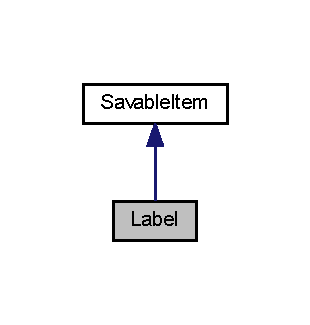
\includegraphics[width=149pt]{class_label__inherit__graph}
\end{center}
\end{figure}


Граф связей класса Label\-:
\nopagebreak
\begin{figure}[H]
\begin{center}
\leavevmode
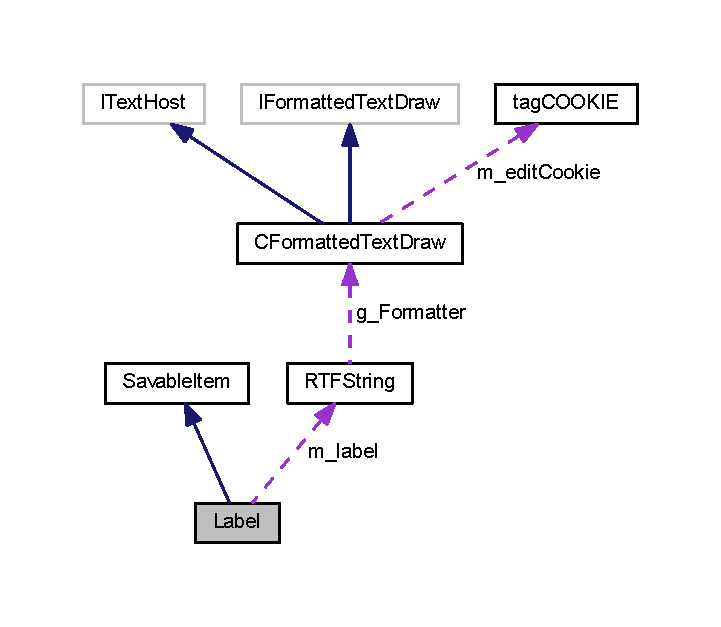
\includegraphics[width=346pt]{class_label__coll__graph}
\end{center}
\end{figure}
\subsection*{Открытые члены}
\begin{DoxyCompactItemize}
\item 
\hyperlink{class_label_ac3c18467d3dbf6f94e94b47c78d4b3c3}{Label} (\hyperlink{class_x_y_plot}{X\-Y\-Plot} $\ast$parent)
\item 
virtual \hyperlink{class_label_a39e1167a9b5827afd888780973d88894}{$\sim$\-Label} ()
\item 
void \hyperlink{class_label_acd24195d832566251e28855717a745be}{Set\-Text} (std\-::string label)
\item 
const std\-::string \& \hyperlink{class_label_aa0d783198414ad2c9a17b7fecfd19581}{Get\-Text} () const 
\item 
void \hyperlink{class_label_a327e98e659b00c708cc41154e65c5f2e}{Set\-Rect} (int left, int top, int right, int bottom)
\item 
void \hyperlink{class_label_a7dd76b7012e10269bb70ebae65c19c20}{Set\-Rect} (R\-E\-C\-T self)
\item 
void \hyperlink{class_label_a585867db26f2a3513cba06fea5fdccff}{Get\-Rect} (R\-E\-C\-T \&self) const 
\item 
S\-I\-Z\-E \hyperlink{class_label_a1c0c60f5aaffb61c7b69e22d3116a305}{Get\-Label\-Size} () const 
\item 
void \hyperlink{class_label_a3d832e782c6821b020fa6a6c3f90b298}{Set\-Style} (D\-W\-O\-R\-D align)
\item 
void \hyperlink{class_label_a2d281ba0d879c5e80dd498b590fde116}{Set\-Font} (const L\-O\-G\-F\-O\-N\-T $\ast$const plf)
\item 
void \hyperlink{class_label_ab35a831ca6da894e091ec422531b819e}{Set\-Color} (C\-O\-L\-O\-R\-R\-E\-F clr)
\item 
B\-O\-O\-L \hyperlink{class_label_af89bd0391480b31547b1793da49cc9eb}{Is\-Enabled} () const 
\item 
void \hyperlink{class_label_a323ad67434f656e25a6e2aa521f9f65f}{Enable} (B\-O\-O\-L enable)
\item 
void \hyperlink{class_label_a39a701c810b83e48ecc6be2ab4a66a19}{Pre\-Draw} (H\-D\-C hdc)
\item 
void \hyperlink{class_label_aa5bdf8574236283b0e0329c5c366cf2f}{On\-Draw} (H\-D\-C hdc)
\item 
virtual B\-O\-O\-L \hyperlink{class_label_a244a940c2d9301bd6bd2abcb2ef9af05}{Write} (H\-A\-N\-D\-L\-E h\-File) const 
\item 
virtual B\-O\-O\-L \hyperlink{class_label_a491dcc38695f69dd135fba56cfdeb3cf}{Read} (H\-A\-N\-D\-L\-E h\-File)
\end{DoxyCompactItemize}
\subsection*{Защищенные данные}
\begin{DoxyCompactItemize}
\item 
D\-W\-O\-R\-D \hyperlink{class_label_ac7c8edd002ef599c40e67831169979f5}{m\-\_\-align}
\item 
\hyperlink{class_r_t_f_string}{R\-T\-F\-String} $\ast$ \hyperlink{class_label_aaf07c83f98530b3f4094107836540fe7}{m\-\_\-label}
\item 
R\-E\-C\-T \hyperlink{class_label_ac8534cb903d21810c0944c0adaa34a5d}{m\-\_\-self}
\item 
B\-O\-O\-L \hyperlink{class_label_a6befb7056ad81ff5790b6bd79361f5a1}{m\-\_\-enabled}
\end{DoxyCompactItemize}
\subsection*{Дополнительные унаследованные члены}


\subsection{Конструктор(ы)}
\hypertarget{class_label_ac3c18467d3dbf6f94e94b47c78d4b3c3}{\index{Label@{Label}!Label@{Label}}
\index{Label@{Label}!Label@{Label}}
\subsubsection[{Label}]{\setlength{\rightskip}{0pt plus 5cm}Label\-::\-Label (
\begin{DoxyParamCaption}
\item[{{\bf X\-Y\-Plot} $\ast$}]{parent}
\end{DoxyParamCaption}
)}}\label{class_label_ac3c18467d3dbf6f94e94b47c78d4b3c3}
\hypertarget{class_label_a39e1167a9b5827afd888780973d88894}{\index{Label@{Label}!$\sim$\-Label@{$\sim$\-Label}}
\index{$\sim$\-Label@{$\sim$\-Label}!Label@{Label}}
\subsubsection[{$\sim$\-Label}]{\setlength{\rightskip}{0pt plus 5cm}Label\-::$\sim$\-Label (
\begin{DoxyParamCaption}
{}
\end{DoxyParamCaption}
)\hspace{0.3cm}{\ttfamily [virtual]}}}\label{class_label_a39e1167a9b5827afd888780973d88894}


\subsection{Методы}
\hypertarget{class_label_a323ad67434f656e25a6e2aa521f9f65f}{\index{Label@{Label}!Enable@{Enable}}
\index{Enable@{Enable}!Label@{Label}}
\subsubsection[{Enable}]{\setlength{\rightskip}{0pt plus 5cm}void Label\-::\-Enable (
\begin{DoxyParamCaption}
\item[{B\-O\-O\-L}]{enable}
\end{DoxyParamCaption}
)\hspace{0.3cm}{\ttfamily [inline]}}}\label{class_label_a323ad67434f656e25a6e2aa521f9f65f}
\hypertarget{class_label_a1c0c60f5aaffb61c7b69e22d3116a305}{\index{Label@{Label}!Get\-Label\-Size@{Get\-Label\-Size}}
\index{Get\-Label\-Size@{Get\-Label\-Size}!Label@{Label}}
\subsubsection[{Get\-Label\-Size}]{\setlength{\rightskip}{0pt plus 5cm}S\-I\-Z\-E Label\-::\-Get\-Label\-Size (
\begin{DoxyParamCaption}
{}
\end{DoxyParamCaption}
) const}}\label{class_label_a1c0c60f5aaffb61c7b69e22d3116a305}
\hypertarget{class_label_a585867db26f2a3513cba06fea5fdccff}{\index{Label@{Label}!Get\-Rect@{Get\-Rect}}
\index{Get\-Rect@{Get\-Rect}!Label@{Label}}
\subsubsection[{Get\-Rect}]{\setlength{\rightskip}{0pt plus 5cm}void Label\-::\-Get\-Rect (
\begin{DoxyParamCaption}
\item[{R\-E\-C\-T \&}]{self}
\end{DoxyParamCaption}
) const\hspace{0.3cm}{\ttfamily [inline]}}}\label{class_label_a585867db26f2a3513cba06fea5fdccff}
\hypertarget{class_label_aa0d783198414ad2c9a17b7fecfd19581}{\index{Label@{Label}!Get\-Text@{Get\-Text}}
\index{Get\-Text@{Get\-Text}!Label@{Label}}
\subsubsection[{Get\-Text}]{\setlength{\rightskip}{0pt plus 5cm}const std\-::string \& Label\-::\-Get\-Text (
\begin{DoxyParamCaption}
{}
\end{DoxyParamCaption}
) const}}\label{class_label_aa0d783198414ad2c9a17b7fecfd19581}
\hypertarget{class_label_af89bd0391480b31547b1793da49cc9eb}{\index{Label@{Label}!Is\-Enabled@{Is\-Enabled}}
\index{Is\-Enabled@{Is\-Enabled}!Label@{Label}}
\subsubsection[{Is\-Enabled}]{\setlength{\rightskip}{0pt plus 5cm}B\-O\-O\-L Label\-::\-Is\-Enabled (
\begin{DoxyParamCaption}
{}
\end{DoxyParamCaption}
) const\hspace{0.3cm}{\ttfamily [inline]}}}\label{class_label_af89bd0391480b31547b1793da49cc9eb}
\hypertarget{class_label_aa5bdf8574236283b0e0329c5c366cf2f}{\index{Label@{Label}!On\-Draw@{On\-Draw}}
\index{On\-Draw@{On\-Draw}!Label@{Label}}
\subsubsection[{On\-Draw}]{\setlength{\rightskip}{0pt plus 5cm}void Label\-::\-On\-Draw (
\begin{DoxyParamCaption}
\item[{H\-D\-C}]{hdc}
\end{DoxyParamCaption}
)}}\label{class_label_aa5bdf8574236283b0e0329c5c366cf2f}
\hypertarget{class_label_a39a701c810b83e48ecc6be2ab4a66a19}{\index{Label@{Label}!Pre\-Draw@{Pre\-Draw}}
\index{Pre\-Draw@{Pre\-Draw}!Label@{Label}}
\subsubsection[{Pre\-Draw}]{\setlength{\rightskip}{0pt plus 5cm}void Label\-::\-Pre\-Draw (
\begin{DoxyParamCaption}
\item[{H\-D\-C}]{hdc}
\end{DoxyParamCaption}
)}}\label{class_label_a39a701c810b83e48ecc6be2ab4a66a19}
\hypertarget{class_label_a491dcc38695f69dd135fba56cfdeb3cf}{\index{Label@{Label}!Read@{Read}}
\index{Read@{Read}!Label@{Label}}
\subsubsection[{Read}]{\setlength{\rightskip}{0pt plus 5cm}B\-O\-O\-L Label\-::\-Read (
\begin{DoxyParamCaption}
\item[{H\-A\-N\-D\-L\-E}]{h\-File}
\end{DoxyParamCaption}
)\hspace{0.3cm}{\ttfamily [virtual]}}}\label{class_label_a491dcc38695f69dd135fba56cfdeb3cf}


Замещает \hyperlink{class_savable_item_a7eadd16b2cb0652091cc15f596a00fb2}{Savable\-Item}.

\hypertarget{class_label_ab35a831ca6da894e091ec422531b819e}{\index{Label@{Label}!Set\-Color@{Set\-Color}}
\index{Set\-Color@{Set\-Color}!Label@{Label}}
\subsubsection[{Set\-Color}]{\setlength{\rightskip}{0pt plus 5cm}void Label\-::\-Set\-Color (
\begin{DoxyParamCaption}
\item[{C\-O\-L\-O\-R\-R\-E\-F}]{clr}
\end{DoxyParamCaption}
)}}\label{class_label_ab35a831ca6da894e091ec422531b819e}
\hypertarget{class_label_a2d281ba0d879c5e80dd498b590fde116}{\index{Label@{Label}!Set\-Font@{Set\-Font}}
\index{Set\-Font@{Set\-Font}!Label@{Label}}
\subsubsection[{Set\-Font}]{\setlength{\rightskip}{0pt plus 5cm}void Label\-::\-Set\-Font (
\begin{DoxyParamCaption}
\item[{const L\-O\-G\-F\-O\-N\-T $\ast$const}]{plf}
\end{DoxyParamCaption}
)}}\label{class_label_a2d281ba0d879c5e80dd498b590fde116}
\hypertarget{class_label_a327e98e659b00c708cc41154e65c5f2e}{\index{Label@{Label}!Set\-Rect@{Set\-Rect}}
\index{Set\-Rect@{Set\-Rect}!Label@{Label}}
\subsubsection[{Set\-Rect}]{\setlength{\rightskip}{0pt plus 5cm}void Label\-::\-Set\-Rect (
\begin{DoxyParamCaption}
\item[{int}]{left, }
\item[{int}]{top, }
\item[{int}]{right, }
\item[{int}]{bottom}
\end{DoxyParamCaption}
)}}\label{class_label_a327e98e659b00c708cc41154e65c5f2e}
\hypertarget{class_label_a7dd76b7012e10269bb70ebae65c19c20}{\index{Label@{Label}!Set\-Rect@{Set\-Rect}}
\index{Set\-Rect@{Set\-Rect}!Label@{Label}}
\subsubsection[{Set\-Rect}]{\setlength{\rightskip}{0pt plus 5cm}void Label\-::\-Set\-Rect (
\begin{DoxyParamCaption}
\item[{R\-E\-C\-T}]{self}
\end{DoxyParamCaption}
)\hspace{0.3cm}{\ttfamily [inline]}}}\label{class_label_a7dd76b7012e10269bb70ebae65c19c20}
\hypertarget{class_label_a3d832e782c6821b020fa6a6c3f90b298}{\index{Label@{Label}!Set\-Style@{Set\-Style}}
\index{Set\-Style@{Set\-Style}!Label@{Label}}
\subsubsection[{Set\-Style}]{\setlength{\rightskip}{0pt plus 5cm}void Label\-::\-Set\-Style (
\begin{DoxyParamCaption}
\item[{D\-W\-O\-R\-D}]{align}
\end{DoxyParamCaption}
)}}\label{class_label_a3d832e782c6821b020fa6a6c3f90b298}
\hypertarget{class_label_acd24195d832566251e28855717a745be}{\index{Label@{Label}!Set\-Text@{Set\-Text}}
\index{Set\-Text@{Set\-Text}!Label@{Label}}
\subsubsection[{Set\-Text}]{\setlength{\rightskip}{0pt plus 5cm}void Label\-::\-Set\-Text (
\begin{DoxyParamCaption}
\item[{std\-::string}]{label}
\end{DoxyParamCaption}
)}}\label{class_label_acd24195d832566251e28855717a745be}
\hypertarget{class_label_a244a940c2d9301bd6bd2abcb2ef9af05}{\index{Label@{Label}!Write@{Write}}
\index{Write@{Write}!Label@{Label}}
\subsubsection[{Write}]{\setlength{\rightskip}{0pt plus 5cm}B\-O\-O\-L Label\-::\-Write (
\begin{DoxyParamCaption}
\item[{H\-A\-N\-D\-L\-E}]{h\-File}
\end{DoxyParamCaption}
) const\hspace{0.3cm}{\ttfamily [virtual]}}}\label{class_label_a244a940c2d9301bd6bd2abcb2ef9af05}


Замещает \hyperlink{class_savable_item_a0da511a4854f515096f8f9b498f64158}{Savable\-Item}.



\subsection{Данные класса}
\hypertarget{class_label_ac7c8edd002ef599c40e67831169979f5}{\index{Label@{Label}!m\-\_\-align@{m\-\_\-align}}
\index{m\-\_\-align@{m\-\_\-align}!Label@{Label}}
\subsubsection[{m\-\_\-align}]{\setlength{\rightskip}{0pt plus 5cm}D\-W\-O\-R\-D Label\-::m\-\_\-align\hspace{0.3cm}{\ttfamily [protected]}}}\label{class_label_ac7c8edd002ef599c40e67831169979f5}
\hypertarget{class_label_a6befb7056ad81ff5790b6bd79361f5a1}{\index{Label@{Label}!m\-\_\-enabled@{m\-\_\-enabled}}
\index{m\-\_\-enabled@{m\-\_\-enabled}!Label@{Label}}
\subsubsection[{m\-\_\-enabled}]{\setlength{\rightskip}{0pt plus 5cm}B\-O\-O\-L Label\-::m\-\_\-enabled\hspace{0.3cm}{\ttfamily [protected]}}}\label{class_label_a6befb7056ad81ff5790b6bd79361f5a1}
\hypertarget{class_label_aaf07c83f98530b3f4094107836540fe7}{\index{Label@{Label}!m\-\_\-label@{m\-\_\-label}}
\index{m\-\_\-label@{m\-\_\-label}!Label@{Label}}
\subsubsection[{m\-\_\-label}]{\setlength{\rightskip}{0pt plus 5cm}{\bf R\-T\-F\-String}$\ast$ Label\-::m\-\_\-label\hspace{0.3cm}{\ttfamily [protected]}}}\label{class_label_aaf07c83f98530b3f4094107836540fe7}
\hypertarget{class_label_ac8534cb903d21810c0944c0adaa34a5d}{\index{Label@{Label}!m\-\_\-self@{m\-\_\-self}}
\index{m\-\_\-self@{m\-\_\-self}!Label@{Label}}
\subsubsection[{m\-\_\-self}]{\setlength{\rightskip}{0pt plus 5cm}R\-E\-C\-T Label\-::m\-\_\-self\hspace{0.3cm}{\ttfamily [protected]}}}\label{class_label_ac8534cb903d21810c0944c0adaa34a5d}


Объявления и описания членов классов находятся в файлах\-:\begin{DoxyCompactItemize}
\item 
src/\hyperlink{label_8h}{label.\-h}\item 
src/\hyperlink{label_8cpp}{label.\-cpp}\end{DoxyCompactItemize}

\hypertarget{class_legend}{\section{Класс Legend}
\label{class_legend}\index{Legend@{Legend}}
}


{\ttfamily \#include $<$legend.\-h$>$}



Граф наследования\-:Legend\-:
\nopagebreak
\begin{figure}[H]
\begin{center}
\leavevmode
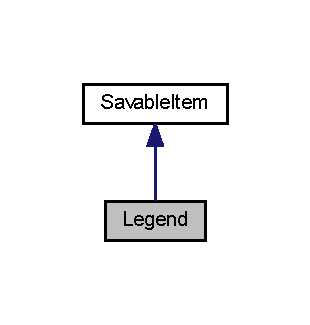
\includegraphics[width=149pt]{class_legend__inherit__graph}
\end{center}
\end{figure}


Граф связей класса Legend\-:
\nopagebreak
\begin{figure}[H]
\begin{center}
\leavevmode
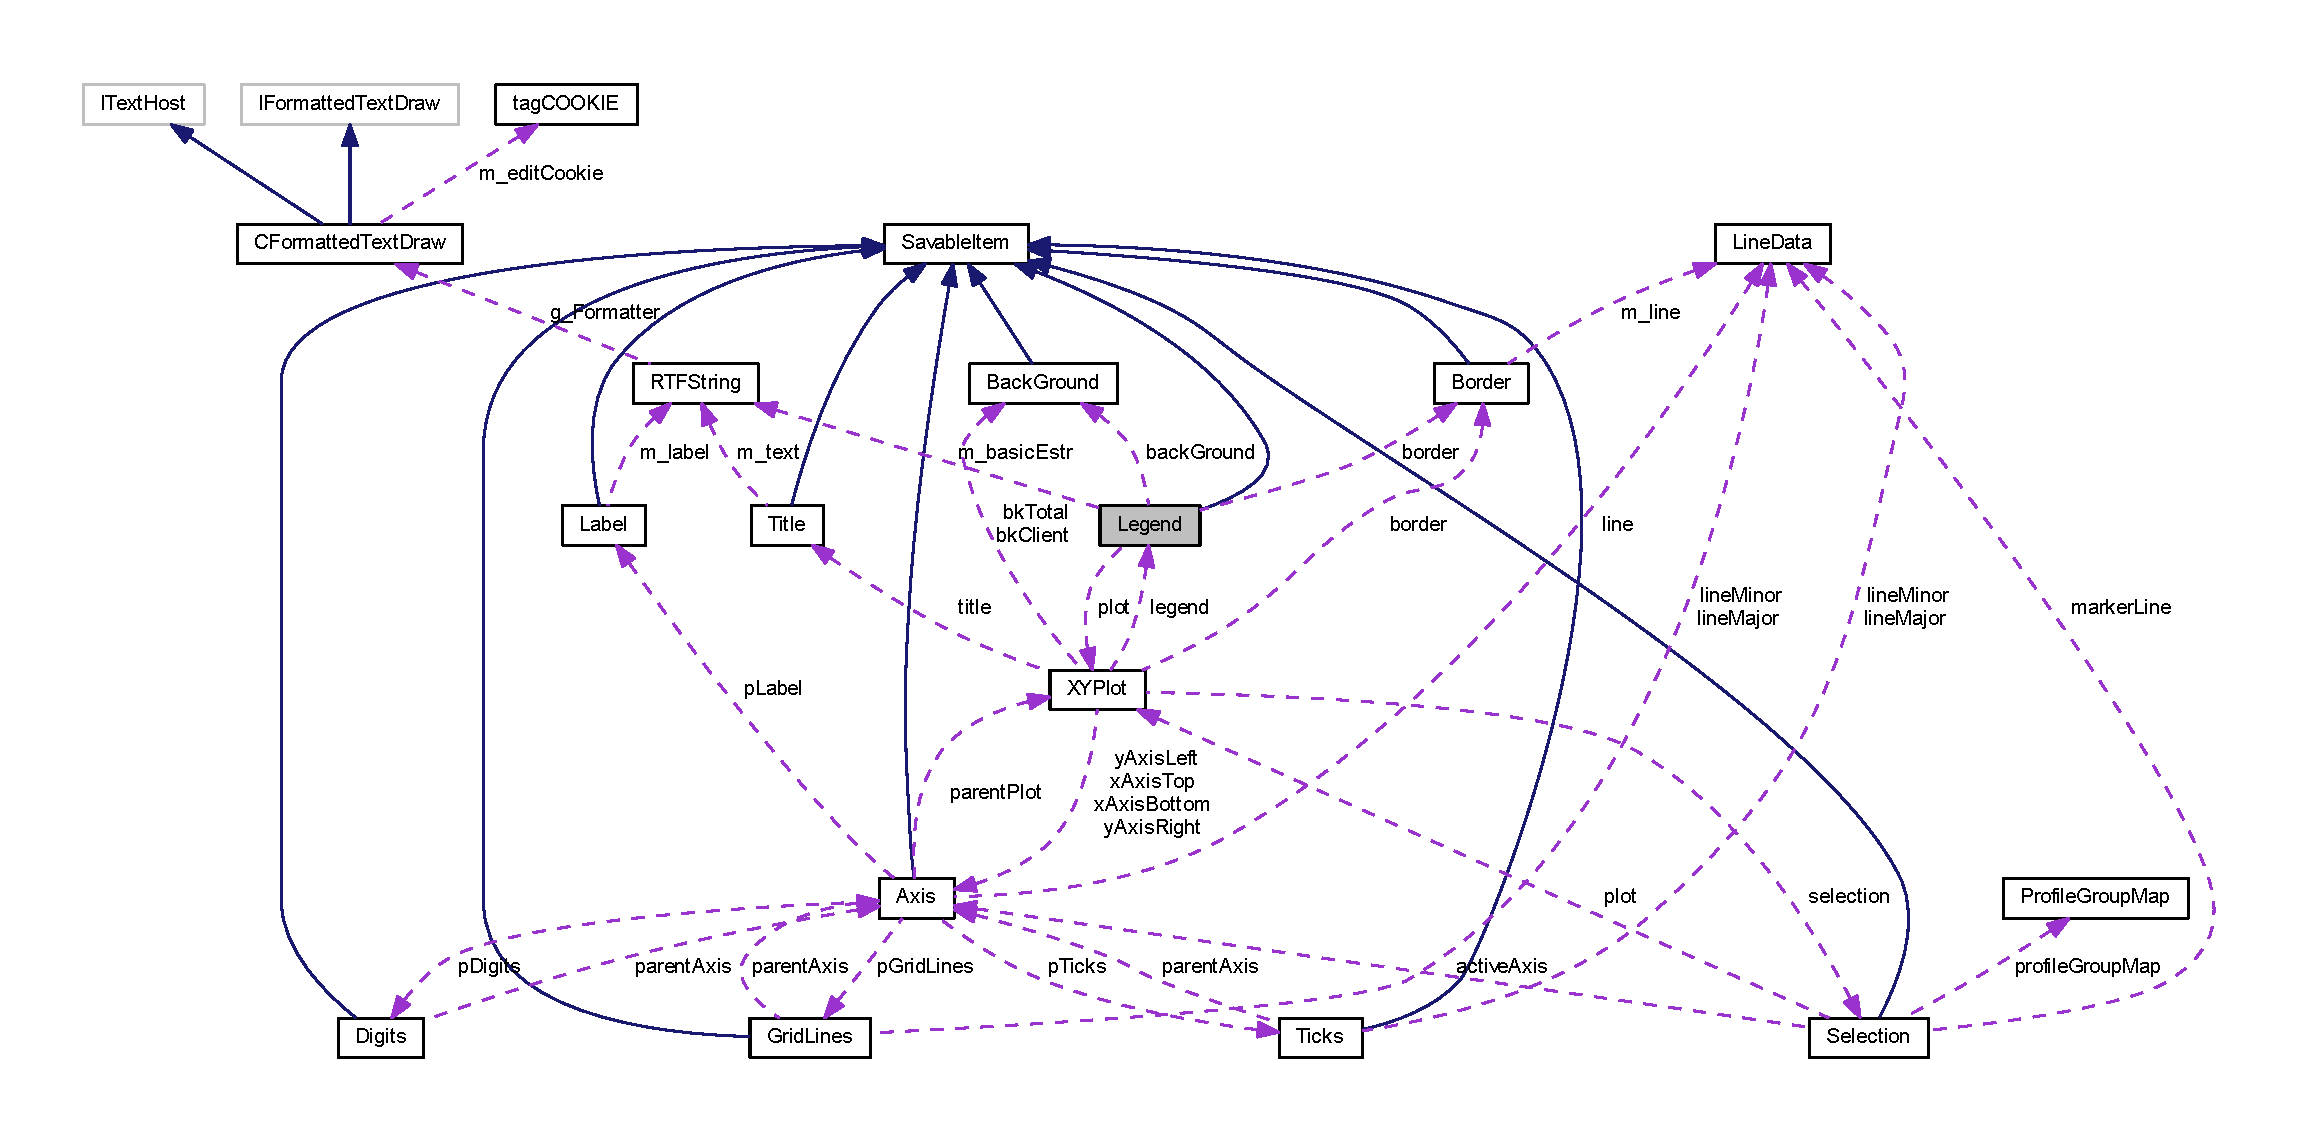
\includegraphics[width=350pt]{class_legend__coll__graph}
\end{center}
\end{figure}
\subsection*{Открытые члены}
\begin{DoxyCompactItemize}
\item 
\hyperlink{class_legend_a4f7f9fbc734a17fcec1aac7d1a8fadd1}{Legend} (\hyperlink{class_x_y_plot}{X\-Y\-Plot} $\ast$parent)
\item 
virtual \hyperlink{class_legend_a115704c32c3ebb783c3ebdd9b2d42f94}{$\sim$\-Legend} ()
\item 
B\-O\-O\-L \hyperlink{class_legend_a0897a355c053f7f6cdf1402e3efc47db}{Is\-Enabled} () const 
\item 
void \hyperlink{class_legend_a54ddf99906fffb8c980460a2b83af3b3}{Enable} (B\-O\-O\-L enable)
\item 
B\-O\-O\-L \hyperlink{class_legend_ad9203ba4dd99cff8f06bfe67a83d177b}{Is\-Hidden} () const 
\item 
void \hyperlink{class_legend_ac0d117f614faf8abc3a0c6662298e331}{Hide} (B\-O\-O\-L hide)
\item 
void \hyperlink{class_legend_a1b6519b466a61a4c41b21c3bbf3d5143}{Set\-Align} (int align)
\item 
int \hyperlink{class_legend_a047bb7503a5efcca94fbf869b535979c}{Get\-Align} () const 
\item 
void \hyperlink{class_legend_a5c9f1626236b331c440ee630e32e2543}{Set\-Rect} (const R\-E\-C\-T \&self)
\item 
void \hyperlink{class_legend_a49b632e529f71ebc6ff9ed337eb46820}{Set\-Rect} (int left, int top, int right, int bottom)
\item 
void \hyperlink{class_legend_a1e5d3d80a9db05979396b7f7d8aaeb24}{Get\-Rect} (R\-E\-C\-T \&self) const 
\item 
void \hyperlink{class_legend_aaaac5b1cc325b70ed985b5e671219be2}{Set\-Cell\-Size} (int width, int height)
\item 
void \hyperlink{class_legend_aa85e5a1690d0b39faa1b93d67027c33d}{Get\-Cell\-Size} (int \&width, int \&height) const 
\item 
void \hyperlink{class_legend_a24fa9da3d1d681d0b668cdbe246852bf}{Set\-Line\-Length} (int length)
\item 
int \hyperlink{class_legend_ad2d3feab72270972696612a660c36c80}{Get\-Line\-Length} () const 
\item 
void \hyperlink{class_legend_a9f1846fd3945025e00c257b30eb83308}{Set\-Font} (const L\-O\-G\-F\-O\-N\-T $\ast$plf)
\item 
void \hyperlink{class_legend_abf18606ec15b245411814d483bf6c84b}{Pre\-Draw} (H\-D\-C hdc, R\-E\-C\-T $\ast$ptotal)
\item 
void \hyperlink{class_legend_aff5b6aaef5b636e6276236ed65e8c1d8}{On\-Draw} (H\-D\-C hdc)
\item 
\hyperlink{profile_8h_ab564cd67657a739c9e5a6caa0ce0dafa}{P\-R\-O\-F\-I\-L\-E\-\_\-\-K\-E\-Y} \hyperlink{class_legend_afc3e60bb5661a763719cdd2a70065fc5}{Hit\-Test} (const P\-O\-I\-N\-T \&pt\-Hit)
\item 
B\-O\-O\-L \hyperlink{class_legend_ac455ef2bd4f20e8889898f02e6c0cc80}{Point\-In\-Rect} (const P\-O\-I\-N\-T \&pt)
\item 
virtual B\-O\-O\-L \hyperlink{class_legend_a93f2a8366a6c5df1b99d4ba2805928b4}{Write} (H\-A\-N\-D\-L\-E h\-File) const 
\item 
virtual B\-O\-O\-L \hyperlink{class_legend_a881509fdd919ed3a30ca822a5edb1114}{Read} (H\-A\-N\-D\-L\-E h\-File)
\end{DoxyCompactItemize}
\subsection*{Защищенные члены}
\begin{DoxyCompactItemize}
\item 
void \hyperlink{class_legend_ae74cfd587be862b4e655bdee5ea08810}{Clear} ()
\end{DoxyCompactItemize}
\subsection*{Защищенные данные}
\begin{DoxyCompactItemize}
\item 
int \hyperlink{class_legend_a63abb8f699af6d3506bc7c8ded4037e0}{m\-\_\-\-Legend\-Offset}
\item 
\hyperlink{class_r_t_f_string}{R\-T\-F\-String} $\ast$ \hyperlink{class_legend_ac52c5c0196d7bddcfab650383f3c88b0}{m\-\_\-basic\-Estr}
\item 
std\-::set$<$ \hyperlink{class_profile}{Profile} $\ast$, \hyperlink{structprofile__less}{profile\-\_\-less} $>$ \hyperlink{class_legend_a418c058072c59c8d2c491852ef3f143b}{profiles}
\item 
const \hyperlink{class_x_y_plot}{X\-Y\-Plot} \& \hyperlink{class_legend_ad033e64a43cceb124ce7b626bdfb695b}{plot}
\item 
\hyperlink{class_border}{Border} \hyperlink{class_legend_ae32f4bc2a9d78cfa069cb242f88cc8f4}{border}
\item 
\hyperlink{class_back_ground}{Back\-Ground} \hyperlink{class_legend_a484eefc380044280c4d44642985293e2}{back\-Ground}
\item 
B\-O\-O\-L \hyperlink{class_legend_a59cedd9de67888759ff39d3fd7c5be45}{m\-\_\-enabled}
\item 
B\-O\-O\-L \hyperlink{class_legend_a7d66848a4111a6a2c0b1fce8ced7d334}{m\-\_\-hidden}
\item 
int \hyperlink{class_legend_a144934b57a8e04a335e6f0d8a39eeb84}{m\-\_\-align}
\item 
R\-E\-C\-T \hyperlink{class_legend_a501285ae1b14654e5ae6a03f7ed4685f}{m\-\_\-self}
\item 
int \hyperlink{class_legend_ac20e23ef899c49a723227dadc21852d0}{m\-\_\-n\-Lines\-Count}
\item 
int \hyperlink{class_legend_a618f51c269707325f1d5a9b20f5544cb}{m\-\_\-cell\-Width}
\item 
int \hyperlink{class_legend_ae505590bc82b4c57bc1af903855490a5}{m\-\_\-cell\-Height}
\item 
int \hyperlink{class_legend_aa5fe3f497876f93e38faa9b248a36fb3}{m\-\_\-line\-Length}
\end{DoxyCompactItemize}
\subsection*{Дополнительные унаследованные члены}


\subsection{Конструктор(ы)}
\hypertarget{class_legend_a4f7f9fbc734a17fcec1aac7d1a8fadd1}{\index{Legend@{Legend}!Legend@{Legend}}
\index{Legend@{Legend}!Legend@{Legend}}
\subsubsection[{Legend}]{\setlength{\rightskip}{0pt plus 5cm}Legend\-::\-Legend (
\begin{DoxyParamCaption}
\item[{{\bf X\-Y\-Plot} $\ast$}]{parent}
\end{DoxyParamCaption}
)}}\label{class_legend_a4f7f9fbc734a17fcec1aac7d1a8fadd1}
\hypertarget{class_legend_a115704c32c3ebb783c3ebdd9b2d42f94}{\index{Legend@{Legend}!$\sim$\-Legend@{$\sim$\-Legend}}
\index{$\sim$\-Legend@{$\sim$\-Legend}!Legend@{Legend}}
\subsubsection[{$\sim$\-Legend}]{\setlength{\rightskip}{0pt plus 5cm}Legend\-::$\sim$\-Legend (
\begin{DoxyParamCaption}
{}
\end{DoxyParamCaption}
)\hspace{0.3cm}{\ttfamily [virtual]}}}\label{class_legend_a115704c32c3ebb783c3ebdd9b2d42f94}


\subsection{Методы}
\hypertarget{class_legend_ae74cfd587be862b4e655bdee5ea08810}{\index{Legend@{Legend}!Clear@{Clear}}
\index{Clear@{Clear}!Legend@{Legend}}
\subsubsection[{Clear}]{\setlength{\rightskip}{0pt plus 5cm}void Legend\-::\-Clear (
\begin{DoxyParamCaption}
{}
\end{DoxyParamCaption}
)\hspace{0.3cm}{\ttfamily [protected]}}}\label{class_legend_ae74cfd587be862b4e655bdee5ea08810}
\hypertarget{class_legend_a54ddf99906fffb8c980460a2b83af3b3}{\index{Legend@{Legend}!Enable@{Enable}}
\index{Enable@{Enable}!Legend@{Legend}}
\subsubsection[{Enable}]{\setlength{\rightskip}{0pt plus 5cm}void Legend\-::\-Enable (
\begin{DoxyParamCaption}
\item[{B\-O\-O\-L}]{enable}
\end{DoxyParamCaption}
)\hspace{0.3cm}{\ttfamily [inline]}}}\label{class_legend_a54ddf99906fffb8c980460a2b83af3b3}
\hypertarget{class_legend_a047bb7503a5efcca94fbf869b535979c}{\index{Legend@{Legend}!Get\-Align@{Get\-Align}}
\index{Get\-Align@{Get\-Align}!Legend@{Legend}}
\subsubsection[{Get\-Align}]{\setlength{\rightskip}{0pt plus 5cm}int Legend\-::\-Get\-Align (
\begin{DoxyParamCaption}
{}
\end{DoxyParamCaption}
) const\hspace{0.3cm}{\ttfamily [inline]}}}\label{class_legend_a047bb7503a5efcca94fbf869b535979c}
\hypertarget{class_legend_aa85e5a1690d0b39faa1b93d67027c33d}{\index{Legend@{Legend}!Get\-Cell\-Size@{Get\-Cell\-Size}}
\index{Get\-Cell\-Size@{Get\-Cell\-Size}!Legend@{Legend}}
\subsubsection[{Get\-Cell\-Size}]{\setlength{\rightskip}{0pt plus 5cm}void Legend\-::\-Get\-Cell\-Size (
\begin{DoxyParamCaption}
\item[{int \&}]{width, }
\item[{int \&}]{height}
\end{DoxyParamCaption}
) const\hspace{0.3cm}{\ttfamily [inline]}}}\label{class_legend_aa85e5a1690d0b39faa1b93d67027c33d}
\hypertarget{class_legend_ad2d3feab72270972696612a660c36c80}{\index{Legend@{Legend}!Get\-Line\-Length@{Get\-Line\-Length}}
\index{Get\-Line\-Length@{Get\-Line\-Length}!Legend@{Legend}}
\subsubsection[{Get\-Line\-Length}]{\setlength{\rightskip}{0pt plus 5cm}int Legend\-::\-Get\-Line\-Length (
\begin{DoxyParamCaption}
{}
\end{DoxyParamCaption}
) const\hspace{0.3cm}{\ttfamily [inline]}}}\label{class_legend_ad2d3feab72270972696612a660c36c80}
\hypertarget{class_legend_a1e5d3d80a9db05979396b7f7d8aaeb24}{\index{Legend@{Legend}!Get\-Rect@{Get\-Rect}}
\index{Get\-Rect@{Get\-Rect}!Legend@{Legend}}
\subsubsection[{Get\-Rect}]{\setlength{\rightskip}{0pt plus 5cm}void Legend\-::\-Get\-Rect (
\begin{DoxyParamCaption}
\item[{R\-E\-C\-T \&}]{self}
\end{DoxyParamCaption}
) const\hspace{0.3cm}{\ttfamily [inline]}}}\label{class_legend_a1e5d3d80a9db05979396b7f7d8aaeb24}
\hypertarget{class_legend_ac0d117f614faf8abc3a0c6662298e331}{\index{Legend@{Legend}!Hide@{Hide}}
\index{Hide@{Hide}!Legend@{Legend}}
\subsubsection[{Hide}]{\setlength{\rightskip}{0pt plus 5cm}void Legend\-::\-Hide (
\begin{DoxyParamCaption}
\item[{B\-O\-O\-L}]{hide}
\end{DoxyParamCaption}
)\hspace{0.3cm}{\ttfamily [inline]}}}\label{class_legend_ac0d117f614faf8abc3a0c6662298e331}
\hypertarget{class_legend_afc3e60bb5661a763719cdd2a70065fc5}{\index{Legend@{Legend}!Hit\-Test@{Hit\-Test}}
\index{Hit\-Test@{Hit\-Test}!Legend@{Legend}}
\subsubsection[{Hit\-Test}]{\setlength{\rightskip}{0pt plus 5cm}{\bf P\-R\-O\-F\-I\-L\-E\-\_\-\-K\-E\-Y} Legend\-::\-Hit\-Test (
\begin{DoxyParamCaption}
\item[{const P\-O\-I\-N\-T \&}]{pt\-Hit}
\end{DoxyParamCaption}
)}}\label{class_legend_afc3e60bb5661a763719cdd2a70065fc5}
\hypertarget{class_legend_a0897a355c053f7f6cdf1402e3efc47db}{\index{Legend@{Legend}!Is\-Enabled@{Is\-Enabled}}
\index{Is\-Enabled@{Is\-Enabled}!Legend@{Legend}}
\subsubsection[{Is\-Enabled}]{\setlength{\rightskip}{0pt plus 5cm}B\-O\-O\-L Legend\-::\-Is\-Enabled (
\begin{DoxyParamCaption}
{}
\end{DoxyParamCaption}
) const\hspace{0.3cm}{\ttfamily [inline]}}}\label{class_legend_a0897a355c053f7f6cdf1402e3efc47db}
\hypertarget{class_legend_ad9203ba4dd99cff8f06bfe67a83d177b}{\index{Legend@{Legend}!Is\-Hidden@{Is\-Hidden}}
\index{Is\-Hidden@{Is\-Hidden}!Legend@{Legend}}
\subsubsection[{Is\-Hidden}]{\setlength{\rightskip}{0pt plus 5cm}B\-O\-O\-L Legend\-::\-Is\-Hidden (
\begin{DoxyParamCaption}
{}
\end{DoxyParamCaption}
) const\hspace{0.3cm}{\ttfamily [inline]}}}\label{class_legend_ad9203ba4dd99cff8f06bfe67a83d177b}
\hypertarget{class_legend_aff5b6aaef5b636e6276236ed65e8c1d8}{\index{Legend@{Legend}!On\-Draw@{On\-Draw}}
\index{On\-Draw@{On\-Draw}!Legend@{Legend}}
\subsubsection[{On\-Draw}]{\setlength{\rightskip}{0pt plus 5cm}void Legend\-::\-On\-Draw (
\begin{DoxyParamCaption}
\item[{H\-D\-C}]{hdc}
\end{DoxyParamCaption}
)}}\label{class_legend_aff5b6aaef5b636e6276236ed65e8c1d8}
\hypertarget{class_legend_ac455ef2bd4f20e8889898f02e6c0cc80}{\index{Legend@{Legend}!Point\-In\-Rect@{Point\-In\-Rect}}
\index{Point\-In\-Rect@{Point\-In\-Rect}!Legend@{Legend}}
\subsubsection[{Point\-In\-Rect}]{\setlength{\rightskip}{0pt plus 5cm}B\-O\-O\-L Legend\-::\-Point\-In\-Rect (
\begin{DoxyParamCaption}
\item[{const P\-O\-I\-N\-T \&}]{pt}
\end{DoxyParamCaption}
)\hspace{0.3cm}{\ttfamily [inline]}}}\label{class_legend_ac455ef2bd4f20e8889898f02e6c0cc80}
\hypertarget{class_legend_abf18606ec15b245411814d483bf6c84b}{\index{Legend@{Legend}!Pre\-Draw@{Pre\-Draw}}
\index{Pre\-Draw@{Pre\-Draw}!Legend@{Legend}}
\subsubsection[{Pre\-Draw}]{\setlength{\rightskip}{0pt plus 5cm}void Legend\-::\-Pre\-Draw (
\begin{DoxyParamCaption}
\item[{H\-D\-C}]{hdc, }
\item[{R\-E\-C\-T $\ast$}]{ptotal}
\end{DoxyParamCaption}
)}}\label{class_legend_abf18606ec15b245411814d483bf6c84b}
\hypertarget{class_legend_a881509fdd919ed3a30ca822a5edb1114}{\index{Legend@{Legend}!Read@{Read}}
\index{Read@{Read}!Legend@{Legend}}
\subsubsection[{Read}]{\setlength{\rightskip}{0pt plus 5cm}B\-O\-O\-L Legend\-::\-Read (
\begin{DoxyParamCaption}
\item[{H\-A\-N\-D\-L\-E}]{h\-File}
\end{DoxyParamCaption}
)\hspace{0.3cm}{\ttfamily [virtual]}}}\label{class_legend_a881509fdd919ed3a30ca822a5edb1114}


Замещает \hyperlink{class_savable_item_a7eadd16b2cb0652091cc15f596a00fb2}{Savable\-Item}.

\hypertarget{class_legend_a1b6519b466a61a4c41b21c3bbf3d5143}{\index{Legend@{Legend}!Set\-Align@{Set\-Align}}
\index{Set\-Align@{Set\-Align}!Legend@{Legend}}
\subsubsection[{Set\-Align}]{\setlength{\rightskip}{0pt plus 5cm}void Legend\-::\-Set\-Align (
\begin{DoxyParamCaption}
\item[{int}]{align}
\end{DoxyParamCaption}
)\hspace{0.3cm}{\ttfamily [inline]}}}\label{class_legend_a1b6519b466a61a4c41b21c3bbf3d5143}
\hypertarget{class_legend_aaaac5b1cc325b70ed985b5e671219be2}{\index{Legend@{Legend}!Set\-Cell\-Size@{Set\-Cell\-Size}}
\index{Set\-Cell\-Size@{Set\-Cell\-Size}!Legend@{Legend}}
\subsubsection[{Set\-Cell\-Size}]{\setlength{\rightskip}{0pt plus 5cm}void Legend\-::\-Set\-Cell\-Size (
\begin{DoxyParamCaption}
\item[{int}]{width, }
\item[{int}]{height}
\end{DoxyParamCaption}
)\hspace{0.3cm}{\ttfamily [inline]}}}\label{class_legend_aaaac5b1cc325b70ed985b5e671219be2}
\hypertarget{class_legend_a9f1846fd3945025e00c257b30eb83308}{\index{Legend@{Legend}!Set\-Font@{Set\-Font}}
\index{Set\-Font@{Set\-Font}!Legend@{Legend}}
\subsubsection[{Set\-Font}]{\setlength{\rightskip}{0pt plus 5cm}void Legend\-::\-Set\-Font (
\begin{DoxyParamCaption}
\item[{const L\-O\-G\-F\-O\-N\-T $\ast$}]{plf}
\end{DoxyParamCaption}
)}}\label{class_legend_a9f1846fd3945025e00c257b30eb83308}
\hypertarget{class_legend_a24fa9da3d1d681d0b668cdbe246852bf}{\index{Legend@{Legend}!Set\-Line\-Length@{Set\-Line\-Length}}
\index{Set\-Line\-Length@{Set\-Line\-Length}!Legend@{Legend}}
\subsubsection[{Set\-Line\-Length}]{\setlength{\rightskip}{0pt plus 5cm}void Legend\-::\-Set\-Line\-Length (
\begin{DoxyParamCaption}
\item[{int}]{length}
\end{DoxyParamCaption}
)\hspace{0.3cm}{\ttfamily [inline]}}}\label{class_legend_a24fa9da3d1d681d0b668cdbe246852bf}
\hypertarget{class_legend_a5c9f1626236b331c440ee630e32e2543}{\index{Legend@{Legend}!Set\-Rect@{Set\-Rect}}
\index{Set\-Rect@{Set\-Rect}!Legend@{Legend}}
\subsubsection[{Set\-Rect}]{\setlength{\rightskip}{0pt plus 5cm}void Legend\-::\-Set\-Rect (
\begin{DoxyParamCaption}
\item[{const R\-E\-C\-T \&}]{self}
\end{DoxyParamCaption}
)\hspace{0.3cm}{\ttfamily [inline]}}}\label{class_legend_a5c9f1626236b331c440ee630e32e2543}
\hypertarget{class_legend_a49b632e529f71ebc6ff9ed337eb46820}{\index{Legend@{Legend}!Set\-Rect@{Set\-Rect}}
\index{Set\-Rect@{Set\-Rect}!Legend@{Legend}}
\subsubsection[{Set\-Rect}]{\setlength{\rightskip}{0pt plus 5cm}void Legend\-::\-Set\-Rect (
\begin{DoxyParamCaption}
\item[{int}]{left, }
\item[{int}]{top, }
\item[{int}]{right, }
\item[{int}]{bottom}
\end{DoxyParamCaption}
)}}\label{class_legend_a49b632e529f71ebc6ff9ed337eb46820}
\hypertarget{class_legend_a93f2a8366a6c5df1b99d4ba2805928b4}{\index{Legend@{Legend}!Write@{Write}}
\index{Write@{Write}!Legend@{Legend}}
\subsubsection[{Write}]{\setlength{\rightskip}{0pt plus 5cm}B\-O\-O\-L Legend\-::\-Write (
\begin{DoxyParamCaption}
\item[{H\-A\-N\-D\-L\-E}]{h\-File}
\end{DoxyParamCaption}
) const\hspace{0.3cm}{\ttfamily [virtual]}}}\label{class_legend_a93f2a8366a6c5df1b99d4ba2805928b4}


Замещает \hyperlink{class_savable_item_a0da511a4854f515096f8f9b498f64158}{Savable\-Item}.



\subsection{Данные класса}
\hypertarget{class_legend_a484eefc380044280c4d44642985293e2}{\index{Legend@{Legend}!back\-Ground@{back\-Ground}}
\index{back\-Ground@{back\-Ground}!Legend@{Legend}}
\subsubsection[{back\-Ground}]{\setlength{\rightskip}{0pt plus 5cm}{\bf Back\-Ground} Legend\-::back\-Ground\hspace{0.3cm}{\ttfamily [protected]}}}\label{class_legend_a484eefc380044280c4d44642985293e2}
\hypertarget{class_legend_ae32f4bc2a9d78cfa069cb242f88cc8f4}{\index{Legend@{Legend}!border@{border}}
\index{border@{border}!Legend@{Legend}}
\subsubsection[{border}]{\setlength{\rightskip}{0pt plus 5cm}{\bf Border} Legend\-::border\hspace{0.3cm}{\ttfamily [protected]}}}\label{class_legend_ae32f4bc2a9d78cfa069cb242f88cc8f4}
\hypertarget{class_legend_a144934b57a8e04a335e6f0d8a39eeb84}{\index{Legend@{Legend}!m\-\_\-align@{m\-\_\-align}}
\index{m\-\_\-align@{m\-\_\-align}!Legend@{Legend}}
\subsubsection[{m\-\_\-align}]{\setlength{\rightskip}{0pt plus 5cm}int Legend\-::m\-\_\-align\hspace{0.3cm}{\ttfamily [protected]}}}\label{class_legend_a144934b57a8e04a335e6f0d8a39eeb84}
\hypertarget{class_legend_ac52c5c0196d7bddcfab650383f3c88b0}{\index{Legend@{Legend}!m\-\_\-basic\-Estr@{m\-\_\-basic\-Estr}}
\index{m\-\_\-basic\-Estr@{m\-\_\-basic\-Estr}!Legend@{Legend}}
\subsubsection[{m\-\_\-basic\-Estr}]{\setlength{\rightskip}{0pt plus 5cm}{\bf R\-T\-F\-String}$\ast$ Legend\-::m\-\_\-basic\-Estr\hspace{0.3cm}{\ttfamily [protected]}}}\label{class_legend_ac52c5c0196d7bddcfab650383f3c88b0}
\hypertarget{class_legend_ae505590bc82b4c57bc1af903855490a5}{\index{Legend@{Legend}!m\-\_\-cell\-Height@{m\-\_\-cell\-Height}}
\index{m\-\_\-cell\-Height@{m\-\_\-cell\-Height}!Legend@{Legend}}
\subsubsection[{m\-\_\-cell\-Height}]{\setlength{\rightskip}{0pt plus 5cm}int Legend\-::m\-\_\-cell\-Height\hspace{0.3cm}{\ttfamily [protected]}}}\label{class_legend_ae505590bc82b4c57bc1af903855490a5}
\hypertarget{class_legend_a618f51c269707325f1d5a9b20f5544cb}{\index{Legend@{Legend}!m\-\_\-cell\-Width@{m\-\_\-cell\-Width}}
\index{m\-\_\-cell\-Width@{m\-\_\-cell\-Width}!Legend@{Legend}}
\subsubsection[{m\-\_\-cell\-Width}]{\setlength{\rightskip}{0pt plus 5cm}int Legend\-::m\-\_\-cell\-Width\hspace{0.3cm}{\ttfamily [protected]}}}\label{class_legend_a618f51c269707325f1d5a9b20f5544cb}
\hypertarget{class_legend_a59cedd9de67888759ff39d3fd7c5be45}{\index{Legend@{Legend}!m\-\_\-enabled@{m\-\_\-enabled}}
\index{m\-\_\-enabled@{m\-\_\-enabled}!Legend@{Legend}}
\subsubsection[{m\-\_\-enabled}]{\setlength{\rightskip}{0pt plus 5cm}B\-O\-O\-L Legend\-::m\-\_\-enabled\hspace{0.3cm}{\ttfamily [protected]}}}\label{class_legend_a59cedd9de67888759ff39d3fd7c5be45}
\hypertarget{class_legend_a7d66848a4111a6a2c0b1fce8ced7d334}{\index{Legend@{Legend}!m\-\_\-hidden@{m\-\_\-hidden}}
\index{m\-\_\-hidden@{m\-\_\-hidden}!Legend@{Legend}}
\subsubsection[{m\-\_\-hidden}]{\setlength{\rightskip}{0pt plus 5cm}B\-O\-O\-L Legend\-::m\-\_\-hidden\hspace{0.3cm}{\ttfamily [protected]}}}\label{class_legend_a7d66848a4111a6a2c0b1fce8ced7d334}
\hypertarget{class_legend_a63abb8f699af6d3506bc7c8ded4037e0}{\index{Legend@{Legend}!m\-\_\-\-Legend\-Offset@{m\-\_\-\-Legend\-Offset}}
\index{m\-\_\-\-Legend\-Offset@{m\-\_\-\-Legend\-Offset}!Legend@{Legend}}
\subsubsection[{m\-\_\-\-Legend\-Offset}]{\setlength{\rightskip}{0pt plus 5cm}int Legend\-::m\-\_\-\-Legend\-Offset\hspace{0.3cm}{\ttfamily [protected]}}}\label{class_legend_a63abb8f699af6d3506bc7c8ded4037e0}
\hypertarget{class_legend_aa5fe3f497876f93e38faa9b248a36fb3}{\index{Legend@{Legend}!m\-\_\-line\-Length@{m\-\_\-line\-Length}}
\index{m\-\_\-line\-Length@{m\-\_\-line\-Length}!Legend@{Legend}}
\subsubsection[{m\-\_\-line\-Length}]{\setlength{\rightskip}{0pt plus 5cm}int Legend\-::m\-\_\-line\-Length\hspace{0.3cm}{\ttfamily [protected]}}}\label{class_legend_aa5fe3f497876f93e38faa9b248a36fb3}
\hypertarget{class_legend_ac20e23ef899c49a723227dadc21852d0}{\index{Legend@{Legend}!m\-\_\-n\-Lines\-Count@{m\-\_\-n\-Lines\-Count}}
\index{m\-\_\-n\-Lines\-Count@{m\-\_\-n\-Lines\-Count}!Legend@{Legend}}
\subsubsection[{m\-\_\-n\-Lines\-Count}]{\setlength{\rightskip}{0pt plus 5cm}int Legend\-::m\-\_\-n\-Lines\-Count\hspace{0.3cm}{\ttfamily [protected]}}}\label{class_legend_ac20e23ef899c49a723227dadc21852d0}
\hypertarget{class_legend_a501285ae1b14654e5ae6a03f7ed4685f}{\index{Legend@{Legend}!m\-\_\-self@{m\-\_\-self}}
\index{m\-\_\-self@{m\-\_\-self}!Legend@{Legend}}
\subsubsection[{m\-\_\-self}]{\setlength{\rightskip}{0pt plus 5cm}R\-E\-C\-T Legend\-::m\-\_\-self\hspace{0.3cm}{\ttfamily [protected]}}}\label{class_legend_a501285ae1b14654e5ae6a03f7ed4685f}
\hypertarget{class_legend_ad033e64a43cceb124ce7b626bdfb695b}{\index{Legend@{Legend}!plot@{plot}}
\index{plot@{plot}!Legend@{Legend}}
\subsubsection[{plot}]{\setlength{\rightskip}{0pt plus 5cm}const {\bf X\-Y\-Plot}\& Legend\-::plot\hspace{0.3cm}{\ttfamily [protected]}}}\label{class_legend_ad033e64a43cceb124ce7b626bdfb695b}
\hypertarget{class_legend_a418c058072c59c8d2c491852ef3f143b}{\index{Legend@{Legend}!profiles@{profiles}}
\index{profiles@{profiles}!Legend@{Legend}}
\subsubsection[{profiles}]{\setlength{\rightskip}{0pt plus 5cm}std\-::set$<${\bf Profile}$\ast$, {\bf profile\-\_\-less}$>$ Legend\-::profiles\hspace{0.3cm}{\ttfamily [protected]}}}\label{class_legend_a418c058072c59c8d2c491852ef3f143b}


Объявления и описания членов классов находятся в файлах\-:\begin{DoxyCompactItemize}
\item 
src/\hyperlink{legend_8h}{legend.\-h}\item 
src/\hyperlink{legend_8cpp}{legend.\-cpp}\end{DoxyCompactItemize}

\hypertarget{class_level_line}{\section{Класс Level\-Line}
\label{class_level_line}\index{Level\-Line@{Level\-Line}}
}


{\ttfamily \#include $<$Level\-Line.\-h$>$}



Граф связей класса Level\-Line\-:
\nopagebreak
\begin{figure}[H]
\begin{center}
\leavevmode
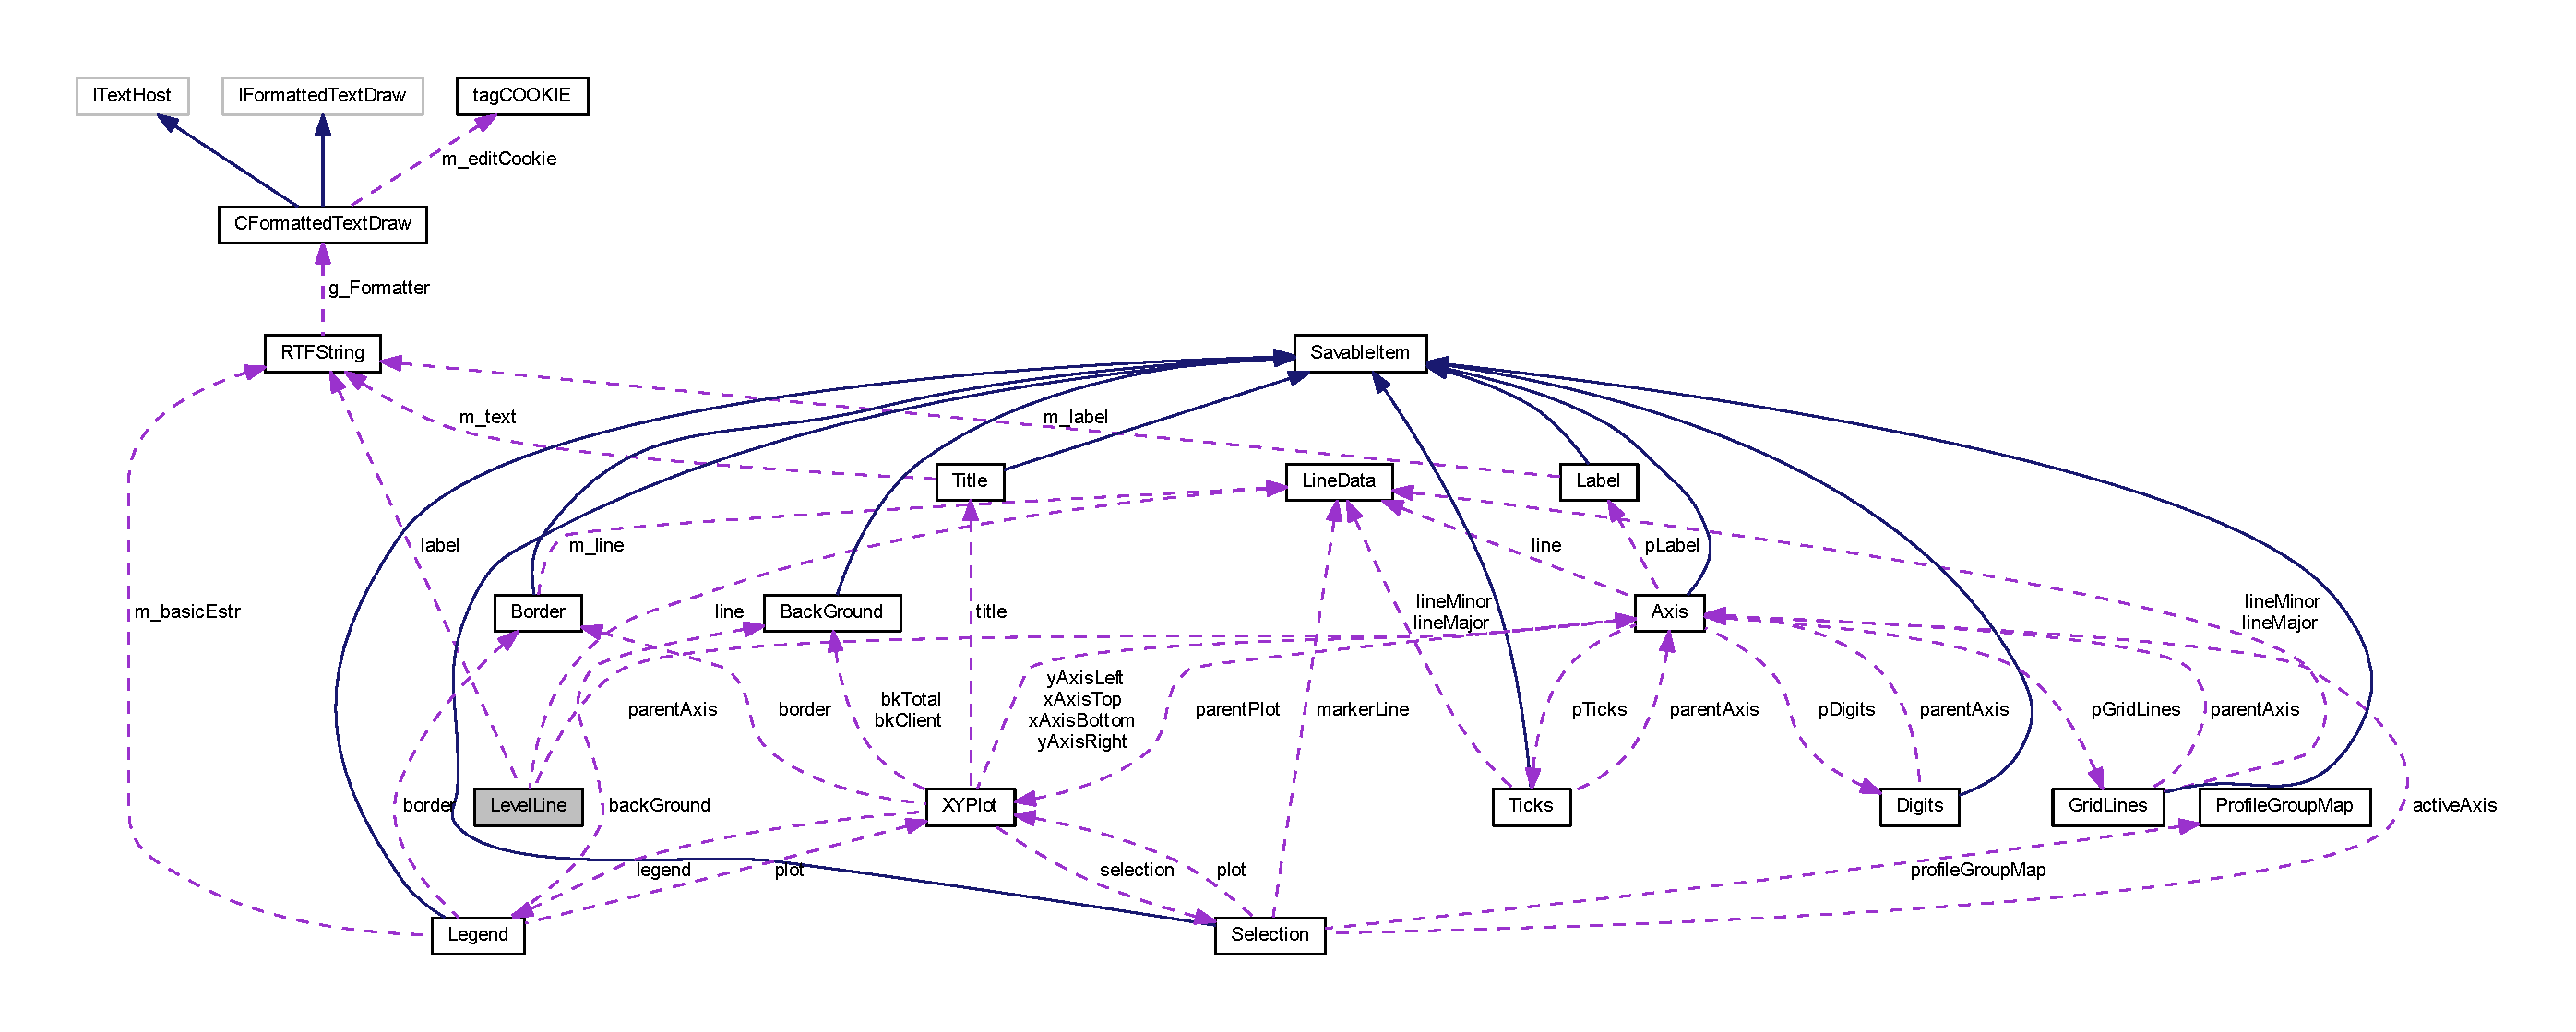
\includegraphics[width=350pt]{class_level_line__coll__graph}
\end{center}
\end{figure}
\subsection*{Открытые члены}
\begin{DoxyCompactItemize}
\item 
\hyperlink{class_level_line_a834a35f51e6cee24e31aa04c122430e9}{Level\-Line} (\hyperlink{class_x_y_plot}{X\-Y\-Plot} $\ast$parent, \hyperlink{class_axis}{Axis} $\ast$\hyperlink{class_level_line_abcbf6e0a95632519d52b3c0828c926f4}{parent\-Axis}, std\-::string label\-Text, C\-O\-L\-O\-R\-R\-E\-F color=0\-L, int Width=2, int Line\-Type=xyplot\-::\-P\-L\-S\-\_\-\-S\-O\-L\-I\-D, double value=0.\-0)
\item 
virtual \hyperlink{class_level_line_ad94c0efb69c76cb12213f658286222c1}{$\sim$\-Level\-Line} ()
\item 
\hyperlink{class_line_data}{Line\-Data} \& \hyperlink{class_level_line_a45589864d3115fbba529533c90c38175}{Get\-Line} ()
\item 
void \hyperlink{class_level_line_a1520645cbe9e84f0904f89eea6e32202}{Set\-Line} (const \hyperlink{class_line_data}{Line\-Data} \&\hyperlink{class_level_line_a98488406c76533a2e70d83197df2614b}{line})
\item 
void \hyperlink{class_level_line_a24695922b2d4ae08dddec50be83800be}{On\-Draw} (H\-D\-C hdc)
\item 
void \hyperlink{class_level_line_a85b3494c4eee0fce6168212dcf903b46}{Set\-Value} (double \hyperlink{class_level_line_ad006f9359dd288a3b189ab964bca9484}{value})
\item 
double \hyperlink{class_level_line_a7c505c12eb4b752f90e52ce77742154a}{Get\-Value} () const 
\item 
const std\-::string \& \hyperlink{class_level_line_a2a9e250359d220d62e1f41b1588201aa}{Get\-Label} () const 
\item 
void \hyperlink{class_level_line_a204f658355806691bc422270f054a6fd}{Set\-Label} (std\-::string)
\item 
void \hyperlink{class_level_line_a089e5b90314f945e221763e1906b031a}{Set\-Label\-Position} (unsigned long \hyperlink{class_level_line_ae4d3c142f618f987e6d7fc35e98e71d0}{pos})
\item 
long \hyperlink{class_level_line_af399e288f9d586a07a6a25250d65470a}{Get\-Label\-Position} ()
\item 
void \hyperlink{class_level_line_a6e10be13208d116ee6d7577b1a68a53e}{Enable\-Label} (B\-O\-O\-L enable=T\-R\-U\-E)
\item 
B\-O\-O\-L \hyperlink{class_level_line_a6c6a0f3b6bc892c63ab0b9d986c9d288}{Is\-Label\-Enabled} ()
\item 
void \hyperlink{class_level_line_a5722ff488016e9a23bb2f17d83d003ca}{Enable} (B\-O\-O\-L enable=T\-R\-U\-E)
\item 
long \hyperlink{class_level_line_a9c4fee2e8c939468ff52fd2204d6fd47}{Get\-Axis\-To\-Attach} ()
\end{DoxyCompactItemize}
\subsection*{Защищенные данные}
\begin{DoxyCompactItemize}
\item 
\hyperlink{class_axis}{Axis} $\ast$ \hyperlink{class_level_line_abcbf6e0a95632519d52b3c0828c926f4}{parent\-Axis}
\item 
double \hyperlink{class_level_line_ad006f9359dd288a3b189ab964bca9484}{value}
\item 
\hyperlink{class_line_data}{Line\-Data} $\ast$ \hyperlink{class_level_line_a98488406c76533a2e70d83197df2614b}{line}
\item 
\hyperlink{class_r_t_f_string}{R\-T\-F\-String} $\ast$ \hyperlink{class_level_line_a8900efadd241d325ed1333a4d4a930d6}{label}
\item 
unsigned long \hyperlink{class_level_line_ae4d3c142f618f987e6d7fc35e98e71d0}{pos}
\item 
B\-O\-O\-L \hyperlink{class_level_line_a76a0fa5a858439419e2cdd49faea7f64}{enabled\-Label}
\item 
B\-O\-O\-L \hyperlink{class_level_line_a887491a0111c8d710fdc491945f80ebb}{enabled}
\end{DoxyCompactItemize}


\subsection{Конструктор(ы)}
\hypertarget{class_level_line_a834a35f51e6cee24e31aa04c122430e9}{\index{Level\-Line@{Level\-Line}!Level\-Line@{Level\-Line}}
\index{Level\-Line@{Level\-Line}!LevelLine@{Level\-Line}}
\subsubsection[{Level\-Line}]{\setlength{\rightskip}{0pt plus 5cm}Level\-Line\-::\-Level\-Line (
\begin{DoxyParamCaption}
\item[{{\bf X\-Y\-Plot} $\ast$}]{parent, }
\item[{{\bf Axis} $\ast$}]{parent\-Axis, }
\item[{std\-::string}]{label\-Text, }
\item[{C\-O\-L\-O\-R\-R\-E\-F}]{color = {\ttfamily 0L}, }
\item[{int}]{Width = {\ttfamily 2}, }
\item[{int}]{Line\-Type = {\ttfamily {\bf xyplot\-::\-P\-L\-S\-\_\-\-S\-O\-L\-I\-D}}, }
\item[{double}]{value = {\ttfamily 0.0}}
\end{DoxyParamCaption}
)}}\label{class_level_line_a834a35f51e6cee24e31aa04c122430e9}
\hypertarget{class_level_line_ad94c0efb69c76cb12213f658286222c1}{\index{Level\-Line@{Level\-Line}!$\sim$\-Level\-Line@{$\sim$\-Level\-Line}}
\index{$\sim$\-Level\-Line@{$\sim$\-Level\-Line}!LevelLine@{Level\-Line}}
\subsubsection[{$\sim$\-Level\-Line}]{\setlength{\rightskip}{0pt plus 5cm}Level\-Line\-::$\sim$\-Level\-Line (
\begin{DoxyParamCaption}
\item[{void}]{}
\end{DoxyParamCaption}
)\hspace{0.3cm}{\ttfamily [virtual]}}}\label{class_level_line_ad94c0efb69c76cb12213f658286222c1}


\subsection{Методы}
\hypertarget{class_level_line_a5722ff488016e9a23bb2f17d83d003ca}{\index{Level\-Line@{Level\-Line}!Enable@{Enable}}
\index{Enable@{Enable}!LevelLine@{Level\-Line}}
\subsubsection[{Enable}]{\setlength{\rightskip}{0pt plus 5cm}void Level\-Line\-::\-Enable (
\begin{DoxyParamCaption}
\item[{B\-O\-O\-L}]{enable = {\ttfamily TRUE}}
\end{DoxyParamCaption}
)\hspace{0.3cm}{\ttfamily [inline]}}}\label{class_level_line_a5722ff488016e9a23bb2f17d83d003ca}
\hypertarget{class_level_line_a6e10be13208d116ee6d7577b1a68a53e}{\index{Level\-Line@{Level\-Line}!Enable\-Label@{Enable\-Label}}
\index{Enable\-Label@{Enable\-Label}!LevelLine@{Level\-Line}}
\subsubsection[{Enable\-Label}]{\setlength{\rightskip}{0pt plus 5cm}void Level\-Line\-::\-Enable\-Label (
\begin{DoxyParamCaption}
\item[{B\-O\-O\-L}]{enable = {\ttfamily TRUE}}
\end{DoxyParamCaption}
)\hspace{0.3cm}{\ttfamily [inline]}}}\label{class_level_line_a6e10be13208d116ee6d7577b1a68a53e}
\hypertarget{class_level_line_a9c4fee2e8c939468ff52fd2204d6fd47}{\index{Level\-Line@{Level\-Line}!Get\-Axis\-To\-Attach@{Get\-Axis\-To\-Attach}}
\index{Get\-Axis\-To\-Attach@{Get\-Axis\-To\-Attach}!LevelLine@{Level\-Line}}
\subsubsection[{Get\-Axis\-To\-Attach}]{\setlength{\rightskip}{0pt plus 5cm}long Level\-Line\-::\-Get\-Axis\-To\-Attach (
\begin{DoxyParamCaption}
{}
\end{DoxyParamCaption}
)}}\label{class_level_line_a9c4fee2e8c939468ff52fd2204d6fd47}
\hypertarget{class_level_line_a2a9e250359d220d62e1f41b1588201aa}{\index{Level\-Line@{Level\-Line}!Get\-Label@{Get\-Label}}
\index{Get\-Label@{Get\-Label}!LevelLine@{Level\-Line}}
\subsubsection[{Get\-Label}]{\setlength{\rightskip}{0pt plus 5cm}const std\-::string \& Level\-Line\-::\-Get\-Label (
\begin{DoxyParamCaption}
{}
\end{DoxyParamCaption}
) const}}\label{class_level_line_a2a9e250359d220d62e1f41b1588201aa}
\hypertarget{class_level_line_af399e288f9d586a07a6a25250d65470a}{\index{Level\-Line@{Level\-Line}!Get\-Label\-Position@{Get\-Label\-Position}}
\index{Get\-Label\-Position@{Get\-Label\-Position}!LevelLine@{Level\-Line}}
\subsubsection[{Get\-Label\-Position}]{\setlength{\rightskip}{0pt plus 5cm}long Level\-Line\-::\-Get\-Label\-Position (
\begin{DoxyParamCaption}
{}
\end{DoxyParamCaption}
)\hspace{0.3cm}{\ttfamily [inline]}}}\label{class_level_line_af399e288f9d586a07a6a25250d65470a}
\hypertarget{class_level_line_a45589864d3115fbba529533c90c38175}{\index{Level\-Line@{Level\-Line}!Get\-Line@{Get\-Line}}
\index{Get\-Line@{Get\-Line}!LevelLine@{Level\-Line}}
\subsubsection[{Get\-Line}]{\setlength{\rightskip}{0pt plus 5cm}{\bf Line\-Data}\& Level\-Line\-::\-Get\-Line (
\begin{DoxyParamCaption}
{}
\end{DoxyParamCaption}
)\hspace{0.3cm}{\ttfamily [inline]}}}\label{class_level_line_a45589864d3115fbba529533c90c38175}
\hypertarget{class_level_line_a7c505c12eb4b752f90e52ce77742154a}{\index{Level\-Line@{Level\-Line}!Get\-Value@{Get\-Value}}
\index{Get\-Value@{Get\-Value}!LevelLine@{Level\-Line}}
\subsubsection[{Get\-Value}]{\setlength{\rightskip}{0pt plus 5cm}double Level\-Line\-::\-Get\-Value (
\begin{DoxyParamCaption}
{}
\end{DoxyParamCaption}
) const\hspace{0.3cm}{\ttfamily [inline]}}}\label{class_level_line_a7c505c12eb4b752f90e52ce77742154a}
\hypertarget{class_level_line_a6c6a0f3b6bc892c63ab0b9d986c9d288}{\index{Level\-Line@{Level\-Line}!Is\-Label\-Enabled@{Is\-Label\-Enabled}}
\index{Is\-Label\-Enabled@{Is\-Label\-Enabled}!LevelLine@{Level\-Line}}
\subsubsection[{Is\-Label\-Enabled}]{\setlength{\rightskip}{0pt plus 5cm}B\-O\-O\-L Level\-Line\-::\-Is\-Label\-Enabled (
\begin{DoxyParamCaption}
{}
\end{DoxyParamCaption}
)\hspace{0.3cm}{\ttfamily [inline]}}}\label{class_level_line_a6c6a0f3b6bc892c63ab0b9d986c9d288}
\hypertarget{class_level_line_a24695922b2d4ae08dddec50be83800be}{\index{Level\-Line@{Level\-Line}!On\-Draw@{On\-Draw}}
\index{On\-Draw@{On\-Draw}!LevelLine@{Level\-Line}}
\subsubsection[{On\-Draw}]{\setlength{\rightskip}{0pt plus 5cm}void Level\-Line\-::\-On\-Draw (
\begin{DoxyParamCaption}
\item[{H\-D\-C}]{hdc}
\end{DoxyParamCaption}
)}}\label{class_level_line_a24695922b2d4ae08dddec50be83800be}
\hypertarget{class_level_line_a204f658355806691bc422270f054a6fd}{\index{Level\-Line@{Level\-Line}!Set\-Label@{Set\-Label}}
\index{Set\-Label@{Set\-Label}!LevelLine@{Level\-Line}}
\subsubsection[{Set\-Label}]{\setlength{\rightskip}{0pt plus 5cm}void Level\-Line\-::\-Set\-Label (
\begin{DoxyParamCaption}
\item[{std\-::string}]{str}
\end{DoxyParamCaption}
)}}\label{class_level_line_a204f658355806691bc422270f054a6fd}
\hypertarget{class_level_line_a089e5b90314f945e221763e1906b031a}{\index{Level\-Line@{Level\-Line}!Set\-Label\-Position@{Set\-Label\-Position}}
\index{Set\-Label\-Position@{Set\-Label\-Position}!LevelLine@{Level\-Line}}
\subsubsection[{Set\-Label\-Position}]{\setlength{\rightskip}{0pt plus 5cm}void Level\-Line\-::\-Set\-Label\-Position (
\begin{DoxyParamCaption}
\item[{unsigned long}]{pos}
\end{DoxyParamCaption}
)\hspace{0.3cm}{\ttfamily [inline]}}}\label{class_level_line_a089e5b90314f945e221763e1906b031a}
\hypertarget{class_level_line_a1520645cbe9e84f0904f89eea6e32202}{\index{Level\-Line@{Level\-Line}!Set\-Line@{Set\-Line}}
\index{Set\-Line@{Set\-Line}!LevelLine@{Level\-Line}}
\subsubsection[{Set\-Line}]{\setlength{\rightskip}{0pt plus 5cm}void Level\-Line\-::\-Set\-Line (
\begin{DoxyParamCaption}
\item[{const {\bf Line\-Data} \&}]{line}
\end{DoxyParamCaption}
)\hspace{0.3cm}{\ttfamily [inline]}}}\label{class_level_line_a1520645cbe9e84f0904f89eea6e32202}
\hypertarget{class_level_line_a85b3494c4eee0fce6168212dcf903b46}{\index{Level\-Line@{Level\-Line}!Set\-Value@{Set\-Value}}
\index{Set\-Value@{Set\-Value}!LevelLine@{Level\-Line}}
\subsubsection[{Set\-Value}]{\setlength{\rightskip}{0pt plus 5cm}void Level\-Line\-::\-Set\-Value (
\begin{DoxyParamCaption}
\item[{double}]{value}
\end{DoxyParamCaption}
)\hspace{0.3cm}{\ttfamily [inline]}}}\label{class_level_line_a85b3494c4eee0fce6168212dcf903b46}


\subsection{Данные класса}
\hypertarget{class_level_line_a887491a0111c8d710fdc491945f80ebb}{\index{Level\-Line@{Level\-Line}!enabled@{enabled}}
\index{enabled@{enabled}!LevelLine@{Level\-Line}}
\subsubsection[{enabled}]{\setlength{\rightskip}{0pt plus 5cm}B\-O\-O\-L Level\-Line\-::enabled\hspace{0.3cm}{\ttfamily [protected]}}}\label{class_level_line_a887491a0111c8d710fdc491945f80ebb}
\hypertarget{class_level_line_a76a0fa5a858439419e2cdd49faea7f64}{\index{Level\-Line@{Level\-Line}!enabled\-Label@{enabled\-Label}}
\index{enabled\-Label@{enabled\-Label}!LevelLine@{Level\-Line}}
\subsubsection[{enabled\-Label}]{\setlength{\rightskip}{0pt plus 5cm}B\-O\-O\-L Level\-Line\-::enabled\-Label\hspace{0.3cm}{\ttfamily [protected]}}}\label{class_level_line_a76a0fa5a858439419e2cdd49faea7f64}
\hypertarget{class_level_line_a8900efadd241d325ed1333a4d4a930d6}{\index{Level\-Line@{Level\-Line}!label@{label}}
\index{label@{label}!LevelLine@{Level\-Line}}
\subsubsection[{label}]{\setlength{\rightskip}{0pt plus 5cm}{\bf R\-T\-F\-String}$\ast$ Level\-Line\-::label\hspace{0.3cm}{\ttfamily [protected]}}}\label{class_level_line_a8900efadd241d325ed1333a4d4a930d6}
\hypertarget{class_level_line_a98488406c76533a2e70d83197df2614b}{\index{Level\-Line@{Level\-Line}!line@{line}}
\index{line@{line}!LevelLine@{Level\-Line}}
\subsubsection[{line}]{\setlength{\rightskip}{0pt plus 5cm}{\bf Line\-Data}$\ast$ Level\-Line\-::line\hspace{0.3cm}{\ttfamily [protected]}}}\label{class_level_line_a98488406c76533a2e70d83197df2614b}
\hypertarget{class_level_line_abcbf6e0a95632519d52b3c0828c926f4}{\index{Level\-Line@{Level\-Line}!parent\-Axis@{parent\-Axis}}
\index{parent\-Axis@{parent\-Axis}!LevelLine@{Level\-Line}}
\subsubsection[{parent\-Axis}]{\setlength{\rightskip}{0pt plus 5cm}{\bf Axis}$\ast$ Level\-Line\-::parent\-Axis\hspace{0.3cm}{\ttfamily [protected]}}}\label{class_level_line_abcbf6e0a95632519d52b3c0828c926f4}
\hypertarget{class_level_line_ae4d3c142f618f987e6d7fc35e98e71d0}{\index{Level\-Line@{Level\-Line}!pos@{pos}}
\index{pos@{pos}!LevelLine@{Level\-Line}}
\subsubsection[{pos}]{\setlength{\rightskip}{0pt plus 5cm}unsigned long Level\-Line\-::pos\hspace{0.3cm}{\ttfamily [protected]}}}\label{class_level_line_ae4d3c142f618f987e6d7fc35e98e71d0}
\hypertarget{class_level_line_ad006f9359dd288a3b189ab964bca9484}{\index{Level\-Line@{Level\-Line}!value@{value}}
\index{value@{value}!LevelLine@{Level\-Line}}
\subsubsection[{value}]{\setlength{\rightskip}{0pt plus 5cm}double Level\-Line\-::value\hspace{0.3cm}{\ttfamily [protected]}}}\label{class_level_line_ad006f9359dd288a3b189ab964bca9484}


Объявления и описания членов классов находятся в файлах\-:\begin{DoxyCompactItemize}
\item 
src/\hyperlink{_level_line_8h}{Level\-Line.\-h}\item 
src/\hyperlink{_level_line_8cpp}{Level\-Line.\-cpp}\end{DoxyCompactItemize}

\hypertarget{struct_font_manager_1_1lf__less}{\section{Структура Font\-Manager\-:\-:lf\-\_\-less}
\label{struct_font_manager_1_1lf__less}\index{Font\-Manager\-::lf\-\_\-less@{Font\-Manager\-::lf\-\_\-less}}
}


{\ttfamily \#include $<$fontmanager.\-h$>$}



Граф наследования\-:Font\-Manager\-:\-:lf\-\_\-less\-:
\nopagebreak
\begin{figure}[H]
\begin{center}
\leavevmode
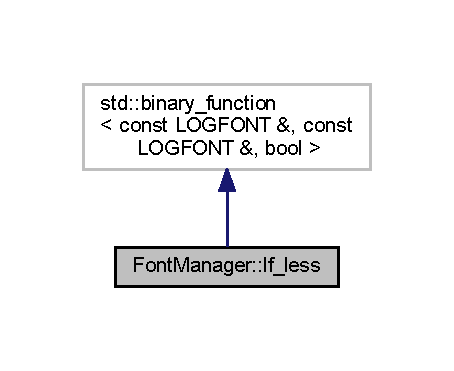
\includegraphics[width=218pt]{struct_font_manager_1_1lf__less__inherit__graph}
\end{center}
\end{figure}


Граф связей класса Font\-Manager\-:\-:lf\-\_\-less\-:
\nopagebreak
\begin{figure}[H]
\begin{center}
\leavevmode
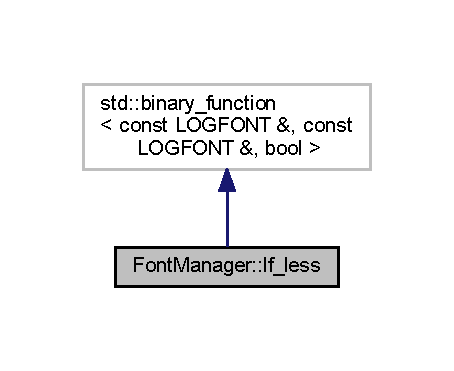
\includegraphics[width=218pt]{struct_font_manager_1_1lf__less__coll__graph}
\end{center}
\end{figure}
\subsection*{Открытые члены}
\begin{DoxyCompactItemize}
\item 
bool \hyperlink{struct_font_manager_1_1lf__less_a9198cbded26fc9c640971b69fb46a54e}{operator()} (const L\-O\-G\-F\-O\-N\-T \&lf, const L\-O\-G\-F\-O\-N\-T \&compare)
\end{DoxyCompactItemize}


\subsection{Методы}
\hypertarget{struct_font_manager_1_1lf__less_a9198cbded26fc9c640971b69fb46a54e}{\index{Font\-Manager\-::lf\-\_\-less@{Font\-Manager\-::lf\-\_\-less}!operator()@{operator()}}
\index{operator()@{operator()}!FontManager::lf_less@{Font\-Manager\-::lf\-\_\-less}}
\subsubsection[{operator()}]{\setlength{\rightskip}{0pt plus 5cm}bool Font\-Manager\-::lf\-\_\-less\-::operator() (
\begin{DoxyParamCaption}
\item[{const L\-O\-G\-F\-O\-N\-T \&}]{lf, }
\item[{const L\-O\-G\-F\-O\-N\-T \&}]{compare}
\end{DoxyParamCaption}
)\hspace{0.3cm}{\ttfamily [inline]}}}\label{struct_font_manager_1_1lf__less_a9198cbded26fc9c640971b69fb46a54e}


Объявления и описания членов структуры находятся в файле\-:\begin{DoxyCompactItemize}
\item 
src/\hyperlink{fontmanager_8h}{fontmanager.\-h}\end{DoxyCompactItemize}

\hypertarget{class_line_data}{\section{Класс Line\-Data}
\label{class_line_data}\index{Line\-Data@{Line\-Data}}
}


{\ttfamily \#include $<$linedata.\-h$>$}

\subsection*{Открытые типы}
\begin{DoxyCompactItemize}
\item 
enum \{ \hyperlink{class_line_data_af2e2ee6851256e24a12203eda9402beaaab3bff3f6a4c9347d819e65d05f5fec3}{R\-O\-U\-N\-D}, 
\hyperlink{class_line_data_af2e2ee6851256e24a12203eda9402beaa396289cd387c745e869339a2c24aedb3}{F\-L\-A\-T}, 
\hyperlink{class_line_data_af2e2ee6851256e24a12203eda9402beaa24fd149f57d8f62d24ffb01013324720}{S\-Q\-U\-A\-R\-E}
 \}
\end{DoxyCompactItemize}
\subsection*{Открытые члены}
\begin{DoxyCompactItemize}
\item 
\hyperlink{class_line_data_af4d6ef9378681b4dd72ccac52c8f4e47}{Line\-Data} ()
\item 
\hyperlink{class_line_data_ac9b85808f69d4f6cfe3741bbfcd65da6}{Line\-Data} (C\-O\-L\-O\-R\-R\-E\-F clr, int n\-Width, int n\-Type, int n\-End\-Caps=\hyperlink{class_line_data_af2e2ee6851256e24a12203eda9402beaaab3bff3f6a4c9347d819e65d05f5fec3}{R\-O\-U\-N\-D}, std\-::string str\-Template=\char`\"{}\char`\"{})
\item 
\hyperlink{class_line_data_a4125b467a9d8d880027c36f8a04ec188}{Line\-Data} (const \hyperlink{class_line_data}{Line\-Data} \&rhs)
\item 
\hyperlink{class_line_data_a8cb45a237eeea2c7c49a8344286e8ab4}{$\sim$\-Line\-Data} ()
\item 
const \hyperlink{class_line_data}{Line\-Data} \& \hyperlink{class_line_data_abb21b7f48aa99ace40cfdff6965fb9df}{operator=} (const \hyperlink{class_line_data}{Line\-Data} \&rhs)
\item 
void \hyperlink{class_line_data_a4590c5b7fb46b8f9194e34ba67642b09}{Set\-Color} (C\-O\-L\-O\-R\-R\-E\-F color)
\item 
C\-O\-L\-O\-R\-R\-E\-F \hyperlink{class_line_data_a207269015f81f59b4dbc32bd402f5d2c}{Get\-Color} () const 
\item 
void \hyperlink{class_line_data_ad60bf3e430a63d31c086c393178c01c5}{Set\-Width} (int n\-Width)
\item 
int \hyperlink{class_line_data_a3fcb7592c8bca72b953fda51b0432d75}{Get\-Width} () const 
\item 
int \hyperlink{class_line_data_af1c04fa13836884d9cb64e8fc3387370}{Set\-Type} (int n\-Type)
\item 
int \hyperlink{class_line_data_af15a08103fa48085eb4ad0ab4888988f}{Get\-Type} () const 
\item 
void \hyperlink{class_line_data_a992ddca82ec4472929a7cf7c613a3619}{Set\-End\-Caps} (int n\-End\-Caps)
\item 
int \hyperlink{class_line_data_ae6cfbcfa7fd82a8a4d4df981cef33f01}{Get\-End\-Caps} () const 
\item 
void \hyperlink{class_line_data_a8ecfe5b4b82f1d4b0d67c1e773b60246}{Set\-Template} (std\-::string str\-Template)
\item 
std\-::string \& \hyperlink{class_line_data_abee244a667b9543d42eb1170fff9682d}{Get\-Template} ()
\item 
\hyperlink{class_line_data_aaaddb4cdac3046ec53caa1e01e91369c}{operator H\-P\-E\-N} ()
\item 
H\-P\-E\-N \hyperlink{class_line_data_a29bc4b864d24ccd29f2edd397f546670}{Get\-Pen} ()
\item 
B\-O\-O\-L \hyperlink{class_line_data_a849c0984d5faba99bb2fa351d6a30801}{Write} (H\-A\-N\-D\-L\-E h\-File) const 
\item 
B\-O\-O\-L \hyperlink{class_line_data_a06d80ee01d05207cf4470dc37662a733}{Read} (H\-A\-N\-D\-L\-E h\-File)
\end{DoxyCompactItemize}
\subsection*{Защищенные члены}
\begin{DoxyCompactItemize}
\item 
void \hyperlink{class_line_data_a95fa94b2614d7058386f82e7c3a2a96d}{Update\-Line\-Template} ()
\item 
void \hyperlink{class_line_data_aeb4bfdd0dc43e28b44efe5726b3b7621}{Create\-Pen} ()
\end{DoxyCompactItemize}
\subsection*{Защищенные данные}
\begin{DoxyCompactItemize}
\item 
int \hyperlink{class_line_data_a67b36139f7b94ec45cbb434cf597ec09}{m\-\_\-type}
\item 
int \hyperlink{class_line_data_a2f510fa43948464d6764fc3e117b5006}{m\-\_\-width}
\item 
int \hyperlink{class_line_data_a671e8aa8a421242fd1a16bf7759220fa}{m\-\_\-end\-Caps}
\item 
C\-O\-L\-O\-R\-R\-E\-F \hyperlink{class_line_data_a641038e14c82d7641df6b1f2e1fd7590}{m\-\_\-color}
\item 
std\-::string \hyperlink{class_line_data_ab1383399938d3d85c3f3b1caa488f322}{m\-\_\-template}
\item 
H\-P\-E\-N \hyperlink{class_line_data_a2774a276fe32645f8d0b44a3032fbf48}{m\-\_\-pen}
\end{DoxyCompactItemize}
\subsection*{Статические защищенные данные}
\begin{DoxyCompactItemize}
\item 
static std\-::string \hyperlink{class_line_data_a19e0f6bc94691eee641daf9a12e37cb0}{D\-A\-S\-H\-T\-E\-M\-P\-L\-A\-T\-E} = \char`\"{}35 20\char`\"{}
\item 
static std\-::string \hyperlink{class_line_data_aabe10496e27e0f52cf6487551c4cb134}{D\-O\-T\-T\-E\-M\-P\-L\-A\-T\-E} = \char`\"{}2 2\char`\"{}
\item 
static std\-::string \hyperlink{class_line_data_aa8a68011b56ff20d76323e1d38929699}{D\-A\-S\-H\-D\-O\-T\-T\-E\-M\-P\-L\-A\-T\-E} = \char`\"{}35 20 7 20\char`\"{}
\item 
static std\-::string \hyperlink{class_line_data_ada248a7a1094de4b553f165ebafb8e9f}{D\-A\-S\-H\-D\-O\-T\-D\-O\-T\-T\-E\-M\-P\-L\-A\-T\-E} = \char`\"{}35 20 7 15 7 20\char`\"{}
\end{DoxyCompactItemize}


\subsection{Перечисления}
\hypertarget{class_line_data_af2e2ee6851256e24a12203eda9402bea}{\subsubsection[{anonymous enum}]{\setlength{\rightskip}{0pt plus 5cm}anonymous enum}}\label{class_line_data_af2e2ee6851256e24a12203eda9402bea}
\begin{Desc}
\item[Элементы перечислений]\par
\begin{description}
\index{R\-O\-U\-N\-D@{R\-O\-U\-N\-D}!Line\-Data@{Line\-Data}}\index{Line\-Data@{Line\-Data}!R\-O\-U\-N\-D@{R\-O\-U\-N\-D}}\item[{\em 
\hypertarget{class_line_data_af2e2ee6851256e24a12203eda9402beaaab3bff3f6a4c9347d819e65d05f5fec3}{R\-O\-U\-N\-D}\label{class_line_data_af2e2ee6851256e24a12203eda9402beaaab3bff3f6a4c9347d819e65d05f5fec3}
}]\index{F\-L\-A\-T@{F\-L\-A\-T}!Line\-Data@{Line\-Data}}\index{Line\-Data@{Line\-Data}!F\-L\-A\-T@{F\-L\-A\-T}}\item[{\em 
\hypertarget{class_line_data_af2e2ee6851256e24a12203eda9402beaa396289cd387c745e869339a2c24aedb3}{F\-L\-A\-T}\label{class_line_data_af2e2ee6851256e24a12203eda9402beaa396289cd387c745e869339a2c24aedb3}
}]\index{S\-Q\-U\-A\-R\-E@{S\-Q\-U\-A\-R\-E}!Line\-Data@{Line\-Data}}\index{Line\-Data@{Line\-Data}!S\-Q\-U\-A\-R\-E@{S\-Q\-U\-A\-R\-E}}\item[{\em 
\hypertarget{class_line_data_af2e2ee6851256e24a12203eda9402beaa24fd149f57d8f62d24ffb01013324720}{S\-Q\-U\-A\-R\-E}\label{class_line_data_af2e2ee6851256e24a12203eda9402beaa24fd149f57d8f62d24ffb01013324720}
}]\end{description}
\end{Desc}


\subsection{Конструктор(ы)}
\hypertarget{class_line_data_af4d6ef9378681b4dd72ccac52c8f4e47}{\index{Line\-Data@{Line\-Data}!Line\-Data@{Line\-Data}}
\index{Line\-Data@{Line\-Data}!LineData@{Line\-Data}}
\subsubsection[{Line\-Data}]{\setlength{\rightskip}{0pt plus 5cm}Line\-Data\-::\-Line\-Data (
\begin{DoxyParamCaption}
{}
\end{DoxyParamCaption}
)}}\label{class_line_data_af4d6ef9378681b4dd72ccac52c8f4e47}
\hypertarget{class_line_data_ac9b85808f69d4f6cfe3741bbfcd65da6}{\index{Line\-Data@{Line\-Data}!Line\-Data@{Line\-Data}}
\index{Line\-Data@{Line\-Data}!LineData@{Line\-Data}}
\subsubsection[{Line\-Data}]{\setlength{\rightskip}{0pt plus 5cm}Line\-Data\-::\-Line\-Data (
\begin{DoxyParamCaption}
\item[{C\-O\-L\-O\-R\-R\-E\-F}]{clr, }
\item[{int}]{n\-Width, }
\item[{int}]{n\-Type, }
\item[{int}]{n\-End\-Caps = {\ttfamily {\bf R\-O\-U\-N\-D}}, }
\item[{std\-::string}]{str\-Template = {\ttfamily \char`\"{}\char`\"{}}}
\end{DoxyParamCaption}
)}}\label{class_line_data_ac9b85808f69d4f6cfe3741bbfcd65da6}
\hypertarget{class_line_data_a4125b467a9d8d880027c36f8a04ec188}{\index{Line\-Data@{Line\-Data}!Line\-Data@{Line\-Data}}
\index{Line\-Data@{Line\-Data}!LineData@{Line\-Data}}
\subsubsection[{Line\-Data}]{\setlength{\rightskip}{0pt plus 5cm}Line\-Data\-::\-Line\-Data (
\begin{DoxyParamCaption}
\item[{const {\bf Line\-Data} \&}]{rhs}
\end{DoxyParamCaption}
)\hspace{0.3cm}{\ttfamily [inline]}}}\label{class_line_data_a4125b467a9d8d880027c36f8a04ec188}
\hypertarget{class_line_data_a8cb45a237eeea2c7c49a8344286e8ab4}{\index{Line\-Data@{Line\-Data}!$\sim$\-Line\-Data@{$\sim$\-Line\-Data}}
\index{$\sim$\-Line\-Data@{$\sim$\-Line\-Data}!LineData@{Line\-Data}}
\subsubsection[{$\sim$\-Line\-Data}]{\setlength{\rightskip}{0pt plus 5cm}Line\-Data\-::$\sim$\-Line\-Data (
\begin{DoxyParamCaption}
{}
\end{DoxyParamCaption}
)}}\label{class_line_data_a8cb45a237eeea2c7c49a8344286e8ab4}


\subsection{Методы}
\hypertarget{class_line_data_aeb4bfdd0dc43e28b44efe5726b3b7621}{\index{Line\-Data@{Line\-Data}!Create\-Pen@{Create\-Pen}}
\index{Create\-Pen@{Create\-Pen}!LineData@{Line\-Data}}
\subsubsection[{Create\-Pen}]{\setlength{\rightskip}{0pt plus 5cm}void Line\-Data\-::\-Create\-Pen (
\begin{DoxyParamCaption}
{}
\end{DoxyParamCaption}
)\hspace{0.3cm}{\ttfamily [protected]}}}\label{class_line_data_aeb4bfdd0dc43e28b44efe5726b3b7621}
\hypertarget{class_line_data_a207269015f81f59b4dbc32bd402f5d2c}{\index{Line\-Data@{Line\-Data}!Get\-Color@{Get\-Color}}
\index{Get\-Color@{Get\-Color}!LineData@{Line\-Data}}
\subsubsection[{Get\-Color}]{\setlength{\rightskip}{0pt plus 5cm}C\-O\-L\-O\-R\-R\-E\-F Line\-Data\-::\-Get\-Color (
\begin{DoxyParamCaption}
{}
\end{DoxyParamCaption}
) const\hspace{0.3cm}{\ttfamily [inline]}}}\label{class_line_data_a207269015f81f59b4dbc32bd402f5d2c}
\hypertarget{class_line_data_ae6cfbcfa7fd82a8a4d4df981cef33f01}{\index{Line\-Data@{Line\-Data}!Get\-End\-Caps@{Get\-End\-Caps}}
\index{Get\-End\-Caps@{Get\-End\-Caps}!LineData@{Line\-Data}}
\subsubsection[{Get\-End\-Caps}]{\setlength{\rightskip}{0pt plus 5cm}int Line\-Data\-::\-Get\-End\-Caps (
\begin{DoxyParamCaption}
{}
\end{DoxyParamCaption}
) const\hspace{0.3cm}{\ttfamily [inline]}}}\label{class_line_data_ae6cfbcfa7fd82a8a4d4df981cef33f01}
\hypertarget{class_line_data_a29bc4b864d24ccd29f2edd397f546670}{\index{Line\-Data@{Line\-Data}!Get\-Pen@{Get\-Pen}}
\index{Get\-Pen@{Get\-Pen}!LineData@{Line\-Data}}
\subsubsection[{Get\-Pen}]{\setlength{\rightskip}{0pt plus 5cm}H\-P\-E\-N Line\-Data\-::\-Get\-Pen (
\begin{DoxyParamCaption}
{}
\end{DoxyParamCaption}
)\hspace{0.3cm}{\ttfamily [inline]}}}\label{class_line_data_a29bc4b864d24ccd29f2edd397f546670}
\hypertarget{class_line_data_abee244a667b9543d42eb1170fff9682d}{\index{Line\-Data@{Line\-Data}!Get\-Template@{Get\-Template}}
\index{Get\-Template@{Get\-Template}!LineData@{Line\-Data}}
\subsubsection[{Get\-Template}]{\setlength{\rightskip}{0pt plus 5cm}std\-::string\& Line\-Data\-::\-Get\-Template (
\begin{DoxyParamCaption}
{}
\end{DoxyParamCaption}
)\hspace{0.3cm}{\ttfamily [inline]}}}\label{class_line_data_abee244a667b9543d42eb1170fff9682d}
\hypertarget{class_line_data_af15a08103fa48085eb4ad0ab4888988f}{\index{Line\-Data@{Line\-Data}!Get\-Type@{Get\-Type}}
\index{Get\-Type@{Get\-Type}!LineData@{Line\-Data}}
\subsubsection[{Get\-Type}]{\setlength{\rightskip}{0pt plus 5cm}int Line\-Data\-::\-Get\-Type (
\begin{DoxyParamCaption}
{}
\end{DoxyParamCaption}
) const\hspace{0.3cm}{\ttfamily [inline]}}}\label{class_line_data_af15a08103fa48085eb4ad0ab4888988f}
\hypertarget{class_line_data_a3fcb7592c8bca72b953fda51b0432d75}{\index{Line\-Data@{Line\-Data}!Get\-Width@{Get\-Width}}
\index{Get\-Width@{Get\-Width}!LineData@{Line\-Data}}
\subsubsection[{Get\-Width}]{\setlength{\rightskip}{0pt plus 5cm}int Line\-Data\-::\-Get\-Width (
\begin{DoxyParamCaption}
{}
\end{DoxyParamCaption}
) const\hspace{0.3cm}{\ttfamily [inline]}}}\label{class_line_data_a3fcb7592c8bca72b953fda51b0432d75}
\hypertarget{class_line_data_aaaddb4cdac3046ec53caa1e01e91369c}{\index{Line\-Data@{Line\-Data}!operator H\-P\-E\-N@{operator H\-P\-E\-N}}
\index{operator H\-P\-E\-N@{operator H\-P\-E\-N}!LineData@{Line\-Data}}
\subsubsection[{operator H\-P\-E\-N}]{\setlength{\rightskip}{0pt plus 5cm}Line\-Data\-::operator H\-P\-E\-N (
\begin{DoxyParamCaption}
{}
\end{DoxyParamCaption}
)\hspace{0.3cm}{\ttfamily [inline]}}}\label{class_line_data_aaaddb4cdac3046ec53caa1e01e91369c}
\hypertarget{class_line_data_abb21b7f48aa99ace40cfdff6965fb9df}{\index{Line\-Data@{Line\-Data}!operator=@{operator=}}
\index{operator=@{operator=}!LineData@{Line\-Data}}
\subsubsection[{operator=}]{\setlength{\rightskip}{0pt plus 5cm}const {\bf Line\-Data} \& Line\-Data\-::operator= (
\begin{DoxyParamCaption}
\item[{const {\bf Line\-Data} \&}]{rhs}
\end{DoxyParamCaption}
)}}\label{class_line_data_abb21b7f48aa99ace40cfdff6965fb9df}
\hypertarget{class_line_data_a06d80ee01d05207cf4470dc37662a733}{\index{Line\-Data@{Line\-Data}!Read@{Read}}
\index{Read@{Read}!LineData@{Line\-Data}}
\subsubsection[{Read}]{\setlength{\rightskip}{0pt plus 5cm}B\-O\-O\-L Line\-Data\-::\-Read (
\begin{DoxyParamCaption}
\item[{H\-A\-N\-D\-L\-E}]{h\-File}
\end{DoxyParamCaption}
)}}\label{class_line_data_a06d80ee01d05207cf4470dc37662a733}
\hypertarget{class_line_data_a4590c5b7fb46b8f9194e34ba67642b09}{\index{Line\-Data@{Line\-Data}!Set\-Color@{Set\-Color}}
\index{Set\-Color@{Set\-Color}!LineData@{Line\-Data}}
\subsubsection[{Set\-Color}]{\setlength{\rightskip}{0pt plus 5cm}void Line\-Data\-::\-Set\-Color (
\begin{DoxyParamCaption}
\item[{C\-O\-L\-O\-R\-R\-E\-F}]{color}
\end{DoxyParamCaption}
)\hspace{0.3cm}{\ttfamily [inline]}}}\label{class_line_data_a4590c5b7fb46b8f9194e34ba67642b09}
\hypertarget{class_line_data_a992ddca82ec4472929a7cf7c613a3619}{\index{Line\-Data@{Line\-Data}!Set\-End\-Caps@{Set\-End\-Caps}}
\index{Set\-End\-Caps@{Set\-End\-Caps}!LineData@{Line\-Data}}
\subsubsection[{Set\-End\-Caps}]{\setlength{\rightskip}{0pt plus 5cm}void Line\-Data\-::\-Set\-End\-Caps (
\begin{DoxyParamCaption}
\item[{int}]{n\-End\-Caps}
\end{DoxyParamCaption}
)\hspace{0.3cm}{\ttfamily [inline]}}}\label{class_line_data_a992ddca82ec4472929a7cf7c613a3619}
\hypertarget{class_line_data_a8ecfe5b4b82f1d4b0d67c1e773b60246}{\index{Line\-Data@{Line\-Data}!Set\-Template@{Set\-Template}}
\index{Set\-Template@{Set\-Template}!LineData@{Line\-Data}}
\subsubsection[{Set\-Template}]{\setlength{\rightskip}{0pt plus 5cm}void Line\-Data\-::\-Set\-Template (
\begin{DoxyParamCaption}
\item[{std\-::string}]{str\-Template}
\end{DoxyParamCaption}
)}}\label{class_line_data_a8ecfe5b4b82f1d4b0d67c1e773b60246}
\hypertarget{class_line_data_af1c04fa13836884d9cb64e8fc3387370}{\index{Line\-Data@{Line\-Data}!Set\-Type@{Set\-Type}}
\index{Set\-Type@{Set\-Type}!LineData@{Line\-Data}}
\subsubsection[{Set\-Type}]{\setlength{\rightskip}{0pt plus 5cm}int Line\-Data\-::\-Set\-Type (
\begin{DoxyParamCaption}
\item[{int}]{n\-Type}
\end{DoxyParamCaption}
)}}\label{class_line_data_af1c04fa13836884d9cb64e8fc3387370}
\hypertarget{class_line_data_ad60bf3e430a63d31c086c393178c01c5}{\index{Line\-Data@{Line\-Data}!Set\-Width@{Set\-Width}}
\index{Set\-Width@{Set\-Width}!LineData@{Line\-Data}}
\subsubsection[{Set\-Width}]{\setlength{\rightskip}{0pt plus 5cm}void Line\-Data\-::\-Set\-Width (
\begin{DoxyParamCaption}
\item[{int}]{n\-Width}
\end{DoxyParamCaption}
)\hspace{0.3cm}{\ttfamily [inline]}}}\label{class_line_data_ad60bf3e430a63d31c086c393178c01c5}
\hypertarget{class_line_data_a95fa94b2614d7058386f82e7c3a2a96d}{\index{Line\-Data@{Line\-Data}!Update\-Line\-Template@{Update\-Line\-Template}}
\index{Update\-Line\-Template@{Update\-Line\-Template}!LineData@{Line\-Data}}
\subsubsection[{Update\-Line\-Template}]{\setlength{\rightskip}{0pt plus 5cm}void Line\-Data\-::\-Update\-Line\-Template (
\begin{DoxyParamCaption}
{}
\end{DoxyParamCaption}
)\hspace{0.3cm}{\ttfamily [protected]}}}\label{class_line_data_a95fa94b2614d7058386f82e7c3a2a96d}
\hypertarget{class_line_data_a849c0984d5faba99bb2fa351d6a30801}{\index{Line\-Data@{Line\-Data}!Write@{Write}}
\index{Write@{Write}!LineData@{Line\-Data}}
\subsubsection[{Write}]{\setlength{\rightskip}{0pt plus 5cm}B\-O\-O\-L Line\-Data\-::\-Write (
\begin{DoxyParamCaption}
\item[{H\-A\-N\-D\-L\-E}]{h\-File}
\end{DoxyParamCaption}
) const}}\label{class_line_data_a849c0984d5faba99bb2fa351d6a30801}


\subsection{Данные класса}
\hypertarget{class_line_data_ada248a7a1094de4b553f165ebafb8e9f}{\index{Line\-Data@{Line\-Data}!D\-A\-S\-H\-D\-O\-T\-D\-O\-T\-T\-E\-M\-P\-L\-A\-T\-E@{D\-A\-S\-H\-D\-O\-T\-D\-O\-T\-T\-E\-M\-P\-L\-A\-T\-E}}
\index{D\-A\-S\-H\-D\-O\-T\-D\-O\-T\-T\-E\-M\-P\-L\-A\-T\-E@{D\-A\-S\-H\-D\-O\-T\-D\-O\-T\-T\-E\-M\-P\-L\-A\-T\-E}!LineData@{Line\-Data}}
\subsubsection[{D\-A\-S\-H\-D\-O\-T\-D\-O\-T\-T\-E\-M\-P\-L\-A\-T\-E}]{\setlength{\rightskip}{0pt plus 5cm}std\-::string Line\-Data\-::\-D\-A\-S\-H\-D\-O\-T\-D\-O\-T\-T\-E\-M\-P\-L\-A\-T\-E = \char`\"{}35 20 7 15 7 20\char`\"{}\hspace{0.3cm}{\ttfamily [static]}, {\ttfamily [protected]}}}\label{class_line_data_ada248a7a1094de4b553f165ebafb8e9f}
\hypertarget{class_line_data_aa8a68011b56ff20d76323e1d38929699}{\index{Line\-Data@{Line\-Data}!D\-A\-S\-H\-D\-O\-T\-T\-E\-M\-P\-L\-A\-T\-E@{D\-A\-S\-H\-D\-O\-T\-T\-E\-M\-P\-L\-A\-T\-E}}
\index{D\-A\-S\-H\-D\-O\-T\-T\-E\-M\-P\-L\-A\-T\-E@{D\-A\-S\-H\-D\-O\-T\-T\-E\-M\-P\-L\-A\-T\-E}!LineData@{Line\-Data}}
\subsubsection[{D\-A\-S\-H\-D\-O\-T\-T\-E\-M\-P\-L\-A\-T\-E}]{\setlength{\rightskip}{0pt plus 5cm}std\-::string Line\-Data\-::\-D\-A\-S\-H\-D\-O\-T\-T\-E\-M\-P\-L\-A\-T\-E = \char`\"{}35 20 7 20\char`\"{}\hspace{0.3cm}{\ttfamily [static]}, {\ttfamily [protected]}}}\label{class_line_data_aa8a68011b56ff20d76323e1d38929699}
\hypertarget{class_line_data_a19e0f6bc94691eee641daf9a12e37cb0}{\index{Line\-Data@{Line\-Data}!D\-A\-S\-H\-T\-E\-M\-P\-L\-A\-T\-E@{D\-A\-S\-H\-T\-E\-M\-P\-L\-A\-T\-E}}
\index{D\-A\-S\-H\-T\-E\-M\-P\-L\-A\-T\-E@{D\-A\-S\-H\-T\-E\-M\-P\-L\-A\-T\-E}!LineData@{Line\-Data}}
\subsubsection[{D\-A\-S\-H\-T\-E\-M\-P\-L\-A\-T\-E}]{\setlength{\rightskip}{0pt plus 5cm}std\-::string Line\-Data\-::\-D\-A\-S\-H\-T\-E\-M\-P\-L\-A\-T\-E = \char`\"{}35 20\char`\"{}\hspace{0.3cm}{\ttfamily [static]}, {\ttfamily [protected]}}}\label{class_line_data_a19e0f6bc94691eee641daf9a12e37cb0}
\hypertarget{class_line_data_aabe10496e27e0f52cf6487551c4cb134}{\index{Line\-Data@{Line\-Data}!D\-O\-T\-T\-E\-M\-P\-L\-A\-T\-E@{D\-O\-T\-T\-E\-M\-P\-L\-A\-T\-E}}
\index{D\-O\-T\-T\-E\-M\-P\-L\-A\-T\-E@{D\-O\-T\-T\-E\-M\-P\-L\-A\-T\-E}!LineData@{Line\-Data}}
\subsubsection[{D\-O\-T\-T\-E\-M\-P\-L\-A\-T\-E}]{\setlength{\rightskip}{0pt plus 5cm}std\-::string Line\-Data\-::\-D\-O\-T\-T\-E\-M\-P\-L\-A\-T\-E = \char`\"{}2 2\char`\"{}\hspace{0.3cm}{\ttfamily [static]}, {\ttfamily [protected]}}}\label{class_line_data_aabe10496e27e0f52cf6487551c4cb134}
\hypertarget{class_line_data_a641038e14c82d7641df6b1f2e1fd7590}{\index{Line\-Data@{Line\-Data}!m\-\_\-color@{m\-\_\-color}}
\index{m\-\_\-color@{m\-\_\-color}!LineData@{Line\-Data}}
\subsubsection[{m\-\_\-color}]{\setlength{\rightskip}{0pt plus 5cm}C\-O\-L\-O\-R\-R\-E\-F Line\-Data\-::m\-\_\-color\hspace{0.3cm}{\ttfamily [protected]}}}\label{class_line_data_a641038e14c82d7641df6b1f2e1fd7590}
\hypertarget{class_line_data_a671e8aa8a421242fd1a16bf7759220fa}{\index{Line\-Data@{Line\-Data}!m\-\_\-end\-Caps@{m\-\_\-end\-Caps}}
\index{m\-\_\-end\-Caps@{m\-\_\-end\-Caps}!LineData@{Line\-Data}}
\subsubsection[{m\-\_\-end\-Caps}]{\setlength{\rightskip}{0pt plus 5cm}int Line\-Data\-::m\-\_\-end\-Caps\hspace{0.3cm}{\ttfamily [protected]}}}\label{class_line_data_a671e8aa8a421242fd1a16bf7759220fa}
\hypertarget{class_line_data_a2774a276fe32645f8d0b44a3032fbf48}{\index{Line\-Data@{Line\-Data}!m\-\_\-pen@{m\-\_\-pen}}
\index{m\-\_\-pen@{m\-\_\-pen}!LineData@{Line\-Data}}
\subsubsection[{m\-\_\-pen}]{\setlength{\rightskip}{0pt plus 5cm}H\-P\-E\-N Line\-Data\-::m\-\_\-pen\hspace{0.3cm}{\ttfamily [protected]}}}\label{class_line_data_a2774a276fe32645f8d0b44a3032fbf48}
\hypertarget{class_line_data_ab1383399938d3d85c3f3b1caa488f322}{\index{Line\-Data@{Line\-Data}!m\-\_\-template@{m\-\_\-template}}
\index{m\-\_\-template@{m\-\_\-template}!LineData@{Line\-Data}}
\subsubsection[{m\-\_\-template}]{\setlength{\rightskip}{0pt plus 5cm}std\-::string Line\-Data\-::m\-\_\-template\hspace{0.3cm}{\ttfamily [protected]}}}\label{class_line_data_ab1383399938d3d85c3f3b1caa488f322}
\hypertarget{class_line_data_a67b36139f7b94ec45cbb434cf597ec09}{\index{Line\-Data@{Line\-Data}!m\-\_\-type@{m\-\_\-type}}
\index{m\-\_\-type@{m\-\_\-type}!LineData@{Line\-Data}}
\subsubsection[{m\-\_\-type}]{\setlength{\rightskip}{0pt plus 5cm}int Line\-Data\-::m\-\_\-type\hspace{0.3cm}{\ttfamily [protected]}}}\label{class_line_data_a67b36139f7b94ec45cbb434cf597ec09}
\hypertarget{class_line_data_a2f510fa43948464d6764fc3e117b5006}{\index{Line\-Data@{Line\-Data}!m\-\_\-width@{m\-\_\-width}}
\index{m\-\_\-width@{m\-\_\-width}!LineData@{Line\-Data}}
\subsubsection[{m\-\_\-width}]{\setlength{\rightskip}{0pt plus 5cm}int Line\-Data\-::m\-\_\-width\hspace{0.3cm}{\ttfamily [protected]}}}\label{class_line_data_a2f510fa43948464d6764fc3e117b5006}


Объявления и описания членов классов находятся в файлах\-:\begin{DoxyCompactItemize}
\item 
src/\hyperlink{linedata_8h}{linedata.\-h}\item 
src/\hyperlink{linedata_8cpp}{linedata.\-cpp}\end{DoxyCompactItemize}

\hypertarget{class_main_critical_section_handler}{\section{Класс Main\-Critical\-Section\-Handler}
\label{class_main_critical_section_handler}\index{Main\-Critical\-Section\-Handler@{Main\-Critical\-Section\-Handler}}
}


{\ttfamily \#include $<$lock.\-h$>$}

\subsection*{Открытые члены}
\begin{DoxyCompactItemize}
\item 
\hyperlink{class_main_critical_section_handler_afceb885a7c66f1eb7270b663aa291732}{Main\-Critical\-Section\-Handler} (L\-P\-C\-R\-I\-T\-I\-C\-A\-L\-\_\-\-S\-E\-C\-T\-I\-O\-N \hyperlink{class_main_critical_section_handler_ae7635d9e5c74721475bf7fbc813e8895}{lpcs})
\item 
\hyperlink{class_main_critical_section_handler_a4f4ebed60b264bd98256363f76285412}{$\sim$\-Main\-Critical\-Section\-Handler} ()
\item 
void \hyperlink{class_main_critical_section_handler_acb1a97f209ca5ebdef5370f514b5b074}{Release} ()
\end{DoxyCompactItemize}
\subsection*{Открытые атрибуты}
\begin{DoxyCompactItemize}
\item 
L\-P\-C\-R\-I\-T\-I\-C\-A\-L\-\_\-\-S\-E\-C\-T\-I\-O\-N \hyperlink{class_main_critical_section_handler_ae7635d9e5c74721475bf7fbc813e8895}{lpcs}
\end{DoxyCompactItemize}


\subsection{Конструктор(ы)}
\hypertarget{class_main_critical_section_handler_afceb885a7c66f1eb7270b663aa291732}{\index{Main\-Critical\-Section\-Handler@{Main\-Critical\-Section\-Handler}!Main\-Critical\-Section\-Handler@{Main\-Critical\-Section\-Handler}}
\index{Main\-Critical\-Section\-Handler@{Main\-Critical\-Section\-Handler}!MainCriticalSectionHandler@{Main\-Critical\-Section\-Handler}}
\subsubsection[{Main\-Critical\-Section\-Handler}]{\setlength{\rightskip}{0pt plus 5cm}Main\-Critical\-Section\-Handler\-::\-Main\-Critical\-Section\-Handler (
\begin{DoxyParamCaption}
\item[{L\-P\-C\-R\-I\-T\-I\-C\-A\-L\-\_\-\-S\-E\-C\-T\-I\-O\-N}]{lpcs}
\end{DoxyParamCaption}
)\hspace{0.3cm}{\ttfamily [inline]}}}\label{class_main_critical_section_handler_afceb885a7c66f1eb7270b663aa291732}
\hypertarget{class_main_critical_section_handler_a4f4ebed60b264bd98256363f76285412}{\index{Main\-Critical\-Section\-Handler@{Main\-Critical\-Section\-Handler}!$\sim$\-Main\-Critical\-Section\-Handler@{$\sim$\-Main\-Critical\-Section\-Handler}}
\index{$\sim$\-Main\-Critical\-Section\-Handler@{$\sim$\-Main\-Critical\-Section\-Handler}!MainCriticalSectionHandler@{Main\-Critical\-Section\-Handler}}
\subsubsection[{$\sim$\-Main\-Critical\-Section\-Handler}]{\setlength{\rightskip}{0pt plus 5cm}Main\-Critical\-Section\-Handler\-::$\sim$\-Main\-Critical\-Section\-Handler (
\begin{DoxyParamCaption}
{}
\end{DoxyParamCaption}
)\hspace{0.3cm}{\ttfamily [inline]}}}\label{class_main_critical_section_handler_a4f4ebed60b264bd98256363f76285412}


\subsection{Методы}
\hypertarget{class_main_critical_section_handler_acb1a97f209ca5ebdef5370f514b5b074}{\index{Main\-Critical\-Section\-Handler@{Main\-Critical\-Section\-Handler}!Release@{Release}}
\index{Release@{Release}!MainCriticalSectionHandler@{Main\-Critical\-Section\-Handler}}
\subsubsection[{Release}]{\setlength{\rightskip}{0pt plus 5cm}void Main\-Critical\-Section\-Handler\-::\-Release (
\begin{DoxyParamCaption}
{}
\end{DoxyParamCaption}
)\hspace{0.3cm}{\ttfamily [inline]}}}\label{class_main_critical_section_handler_acb1a97f209ca5ebdef5370f514b5b074}


\subsection{Данные класса}
\hypertarget{class_main_critical_section_handler_ae7635d9e5c74721475bf7fbc813e8895}{\index{Main\-Critical\-Section\-Handler@{Main\-Critical\-Section\-Handler}!lpcs@{lpcs}}
\index{lpcs@{lpcs}!MainCriticalSectionHandler@{Main\-Critical\-Section\-Handler}}
\subsubsection[{lpcs}]{\setlength{\rightskip}{0pt plus 5cm}L\-P\-C\-R\-I\-T\-I\-C\-A\-L\-\_\-\-S\-E\-C\-T\-I\-O\-N Main\-Critical\-Section\-Handler\-::lpcs}}\label{class_main_critical_section_handler_ae7635d9e5c74721475bf7fbc813e8895}


Объявления и описания членов класса находятся в файле\-:\begin{DoxyCompactItemize}
\item 
src/\hyperlink{lock_8h}{lock.\-h}\end{DoxyCompactItemize}

\hypertarget{classxyplot_1_1_plot_handle}{\section{Класс xyplot\-:\-:Plot\-Handle}
\label{classxyplot_1_1_plot_handle}\index{xyplot\-::\-Plot\-Handle@{xyplot\-::\-Plot\-Handle}}
}


Базовый класс дескрипторов 2\-D графики  




{\ttfamily \#include $<$X\-Y\-Plot\-Wrapper.\-h$>$}



Граф наследования\-:xyplot\-:\-:Plot\-Handle\-:\nopagebreak
\begin{figure}[H]
\begin{center}
\leavevmode
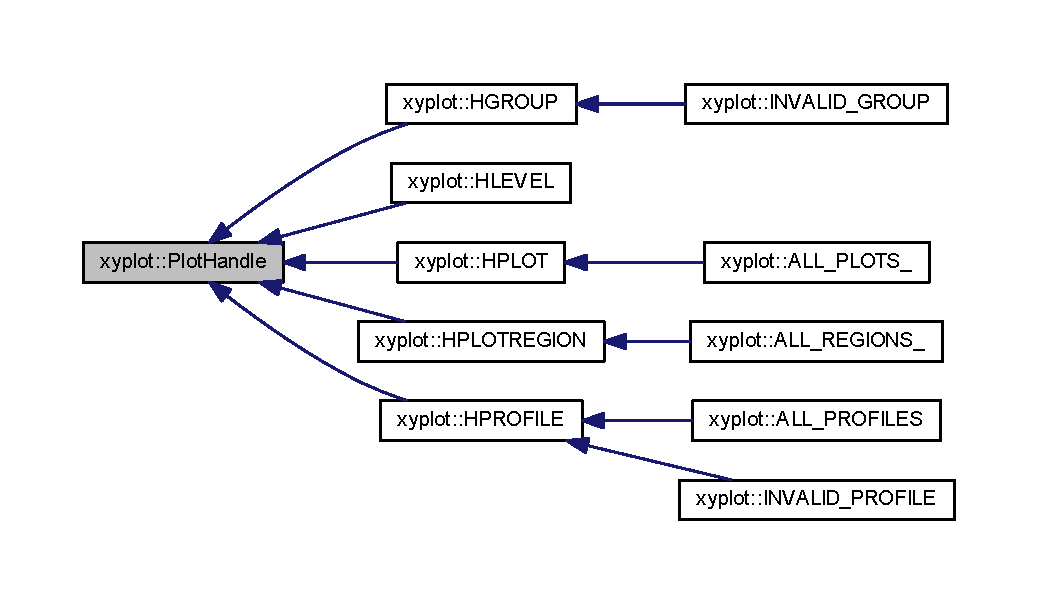
\includegraphics[width=350pt]{classxyplot_1_1_plot_handle__inherit__graph}
\end{center}
\end{figure}
\subsection*{Открытые члены}
\begin{DoxyCompactItemize}
\item 
virtual \hyperlink{classxyplot_1_1_plot_handle_a1aa470b07c0cf1712f15bafdb5fb8a48}{$\sim$\-Plot\-Handle} ()
\item 
const \hyperlink{classxyplot_1_1_plot_handle}{Plot\-Handle} \& \hyperlink{classxyplot_1_1_plot_handle_ab1fd6b3147239c1485a345dc2baadc05}{operator=} (const \hyperlink{classxyplot_1_1_plot_handle}{Plot\-Handle} \&rhs)
\item 
bool \hyperlink{classxyplot_1_1_plot_handle_afd66331f425ea57e0562dfb74a81177b}{operator!} () const 
\item 
bool \hyperlink{classxyplot_1_1_plot_handle_afa7e238ea63f7ab13f24a377aab21282}{operator!=} (const \hyperlink{classxyplot_1_1_plot_handle}{Plot\-Handle} \&rhs) const 
\item 
\hyperlink{classxyplot_1_1_plot_handle_a1fa0bcf721b1b346f7d96230098da3fe}{operator long} () const 
\item 
\hyperlink{namespacexyplot_a27bc71b0bdfac09495e7e531d8a918c5}{long} $\ast$ \hyperlink{classxyplot_1_1_plot_handle_a5372007842b00fea6760f0324ed3220e}{operator\&} ()
\item 
\hyperlink{classxyplot_1_1_plot_handle_ab2004cbf4e4400de4e4413b9b75c281c}{Plot\-Handle} (\hyperlink{namespacexyplot_a27bc71b0bdfac09495e7e531d8a918c5}{long} n)
\item 
\hyperlink{classxyplot_1_1_plot_handle_a5226ba05ba9568584b2ef81fbf76e152}{Plot\-Handle} (const \hyperlink{classxyplot_1_1_plot_handle}{Plot\-Handle} \&rhs)
\end{DoxyCompactItemize}
\subsection*{Защищенные члены}
\begin{DoxyCompactItemize}
\item 
\hyperlink{classxyplot_1_1_plot_handle_afddd74546013d446df5478d72c87eef4}{Plot\-Handle} ()
\end{DoxyCompactItemize}


\subsection{Подробное описание}
Базовый класс дескрипторов 2\-D графики 

\subsection{Конструктор(ы)}
\hypertarget{classxyplot_1_1_plot_handle_a1aa470b07c0cf1712f15bafdb5fb8a48}{\index{xyplot\-::\-Plot\-Handle@{xyplot\-::\-Plot\-Handle}!$\sim$\-Plot\-Handle@{$\sim$\-Plot\-Handle}}
\index{$\sim$\-Plot\-Handle@{$\sim$\-Plot\-Handle}!xyplot::PlotHandle@{xyplot\-::\-Plot\-Handle}}
\subsubsection[{$\sim$\-Plot\-Handle}]{\setlength{\rightskip}{0pt plus 5cm}virtual xyplot\-::\-Plot\-Handle\-::$\sim$\-Plot\-Handle (
\begin{DoxyParamCaption}
{}
\end{DoxyParamCaption}
)\hspace{0.3cm}{\ttfamily [inline]}, {\ttfamily [virtual]}}}\label{classxyplot_1_1_plot_handle_a1aa470b07c0cf1712f15bafdb5fb8a48}
Деструктор \hypertarget{classxyplot_1_1_plot_handle_afddd74546013d446df5478d72c87eef4}{\index{xyplot\-::\-Plot\-Handle@{xyplot\-::\-Plot\-Handle}!Plot\-Handle@{Plot\-Handle}}
\index{Plot\-Handle@{Plot\-Handle}!xyplot::PlotHandle@{xyplot\-::\-Plot\-Handle}}
\subsubsection[{Plot\-Handle}]{\setlength{\rightskip}{0pt plus 5cm}xyplot\-::\-Plot\-Handle\-::\-Plot\-Handle (
\begin{DoxyParamCaption}
{}
\end{DoxyParamCaption}
)\hspace{0.3cm}{\ttfamily [inline]}, {\ttfamily [protected]}}}\label{classxyplot_1_1_plot_handle_afddd74546013d446df5478d72c87eef4}
Конструктор по умолчанию. Инициализирует пустой дескриптор (= 0) \hypertarget{classxyplot_1_1_plot_handle_ab2004cbf4e4400de4e4413b9b75c281c}{\index{xyplot\-::\-Plot\-Handle@{xyplot\-::\-Plot\-Handle}!Plot\-Handle@{Plot\-Handle}}
\index{Plot\-Handle@{Plot\-Handle}!xyplot::PlotHandle@{xyplot\-::\-Plot\-Handle}}
\subsubsection[{Plot\-Handle}]{\setlength{\rightskip}{0pt plus 5cm}xyplot\-::\-Plot\-Handle\-::\-Plot\-Handle (
\begin{DoxyParamCaption}
\item[{{\bf long}}]{n}
\end{DoxyParamCaption}
)\hspace{0.3cm}{\ttfamily [inline]}}}\label{classxyplot_1_1_plot_handle_ab2004cbf4e4400de4e4413b9b75c281c}
Конструктор с параметром. 
\begin{DoxyParams}{Аргументы}
{\em n} & -\/ ??? \\
\hline
\end{DoxyParams}
\hypertarget{classxyplot_1_1_plot_handle_a5226ba05ba9568584b2ef81fbf76e152}{\index{xyplot\-::\-Plot\-Handle@{xyplot\-::\-Plot\-Handle}!Plot\-Handle@{Plot\-Handle}}
\index{Plot\-Handle@{Plot\-Handle}!xyplot::PlotHandle@{xyplot\-::\-Plot\-Handle}}
\subsubsection[{Plot\-Handle}]{\setlength{\rightskip}{0pt plus 5cm}xyplot\-::\-Plot\-Handle\-::\-Plot\-Handle (
\begin{DoxyParamCaption}
\item[{const {\bf Plot\-Handle} \&}]{rhs}
\end{DoxyParamCaption}
)\hspace{0.3cm}{\ttfamily [inline]}}}\label{classxyplot_1_1_plot_handle_a5226ba05ba9568584b2ef81fbf76e152}
Конструктор копирования. 
\begin{DoxyParams}{Аргументы}
{\em rhs} & ссылка на существующий дескриптор \\
\hline
\end{DoxyParams}


\subsection{Методы}
\hypertarget{classxyplot_1_1_plot_handle_a1fa0bcf721b1b346f7d96230098da3fe}{\index{xyplot\-::\-Plot\-Handle@{xyplot\-::\-Plot\-Handle}!operator long@{operator long}}
\index{operator long@{operator long}!xyplot::PlotHandle@{xyplot\-::\-Plot\-Handle}}
\subsubsection[{operator long}]{\setlength{\rightskip}{0pt plus 5cm}xyplot\-::\-Plot\-Handle\-::operator {\bf long} (
\begin{DoxyParamCaption}
{}
\end{DoxyParamCaption}
) const\hspace{0.3cm}{\ttfamily [inline]}}}\label{classxyplot_1_1_plot_handle_a1fa0bcf721b1b346f7d96230098da3fe}
Oператор приведения к {\bfseries long}. \begin{DoxyReturn}{Возвращает}
дескриптор в виде {\bfseries long} 
\end{DoxyReturn}
\hypertarget{classxyplot_1_1_plot_handle_afd66331f425ea57e0562dfb74a81177b}{\index{xyplot\-::\-Plot\-Handle@{xyplot\-::\-Plot\-Handle}!operator!@{operator!}}
\index{operator!@{operator!}!xyplot::PlotHandle@{xyplot\-::\-Plot\-Handle}}
\subsubsection[{operator!}]{\setlength{\rightskip}{0pt plus 5cm}bool xyplot\-::\-Plot\-Handle\-::operator! (
\begin{DoxyParamCaption}
{}
\end{DoxyParamCaption}
) const\hspace{0.3cm}{\ttfamily [inline]}}}\label{classxyplot_1_1_plot_handle_afd66331f425ea57e0562dfb74a81177b}
Оператор логическое нет \begin{DoxyReturn}{Возвращает}
true если дескриптор пустой ( = 0) 

false если дескриптор не нулевой 
\end{DoxyReturn}
\hypertarget{classxyplot_1_1_plot_handle_afa7e238ea63f7ab13f24a377aab21282}{\index{xyplot\-::\-Plot\-Handle@{xyplot\-::\-Plot\-Handle}!operator!=@{operator!=}}
\index{operator!=@{operator!=}!xyplot::PlotHandle@{xyplot\-::\-Plot\-Handle}}
\subsubsection[{operator!=}]{\setlength{\rightskip}{0pt plus 5cm}bool {\bf xyplot\-::\-Plot\-Handle\-::operator!}= (
\begin{DoxyParamCaption}
\item[{const {\bf Plot\-Handle} \&}]{rhs}
\end{DoxyParamCaption}
) const\hspace{0.3cm}{\ttfamily [inline]}}}\label{classxyplot_1_1_plot_handle_afa7e238ea63f7ab13f24a377aab21282}
Оператор не равно. Сравнивает с существующим дескриптором 
\begin{DoxyParams}{Аргументы}
{\em rhs} & ссылка на существующий дескриптор \\
\hline
\end{DoxyParams}
\begin{DoxyReturn}{Возвращает}
true если дескрипторы не равены 

false если дескрипторы равены 
\end{DoxyReturn}
\hypertarget{classxyplot_1_1_plot_handle_a5372007842b00fea6760f0324ed3220e}{\index{xyplot\-::\-Plot\-Handle@{xyplot\-::\-Plot\-Handle}!operator\&@{operator\&}}
\index{operator\&@{operator\&}!xyplot::PlotHandle@{xyplot\-::\-Plot\-Handle}}
\subsubsection[{operator\&}]{\setlength{\rightskip}{0pt plus 5cm}{\bf long}$\ast$ xyplot\-::\-Plot\-Handle\-::operator\& (
\begin{DoxyParamCaption}
{}
\end{DoxyParamCaption}
)\hspace{0.3cm}{\ttfamily [inline]}}}\label{classxyplot_1_1_plot_handle_a5372007842b00fea6760f0324ed3220e}
Унарный оператор \& возвращает адрес дескриптора. \begin{DoxyReturn}{Возвращает}
возвращает адрес дескриптора 
\end{DoxyReturn}
\hypertarget{classxyplot_1_1_plot_handle_ab1fd6b3147239c1485a345dc2baadc05}{\index{xyplot\-::\-Plot\-Handle@{xyplot\-::\-Plot\-Handle}!operator=@{operator=}}
\index{operator=@{operator=}!xyplot::PlotHandle@{xyplot\-::\-Plot\-Handle}}
\subsubsection[{operator=}]{\setlength{\rightskip}{0pt plus 5cm}const {\bf Plot\-Handle}\& xyplot\-::\-Plot\-Handle\-::operator= (
\begin{DoxyParamCaption}
\item[{const {\bf Plot\-Handle} \&}]{rhs}
\end{DoxyParamCaption}
)\hspace{0.3cm}{\ttfamily [inline]}}}\label{classxyplot_1_1_plot_handle_ab1fd6b3147239c1485a345dc2baadc05}
Оператор присваивания 
\begin{DoxyParams}{Аргументы}
{\em rhs} & ссылка на существующий дескриптор \\
\hline
\end{DoxyParams}


Объявления и описания членов класса находятся в файле\-:\begin{DoxyCompactItemize}
\item 
src/\hyperlink{_x_y_plot_wrapper_8h}{X\-Y\-Plot\-Wrapper.\-h}\end{DoxyCompactItemize}

\hypertarget{class_plot_region}{\section{Класс Plot\-Region}
\label{class_plot_region}\index{Plot\-Region@{Plot\-Region}}
}


{\ttfamily \#include $<$Regions.\-h$>$}



Граф связей класса Plot\-Region\-:
\nopagebreak
\begin{figure}[H]
\begin{center}
\leavevmode
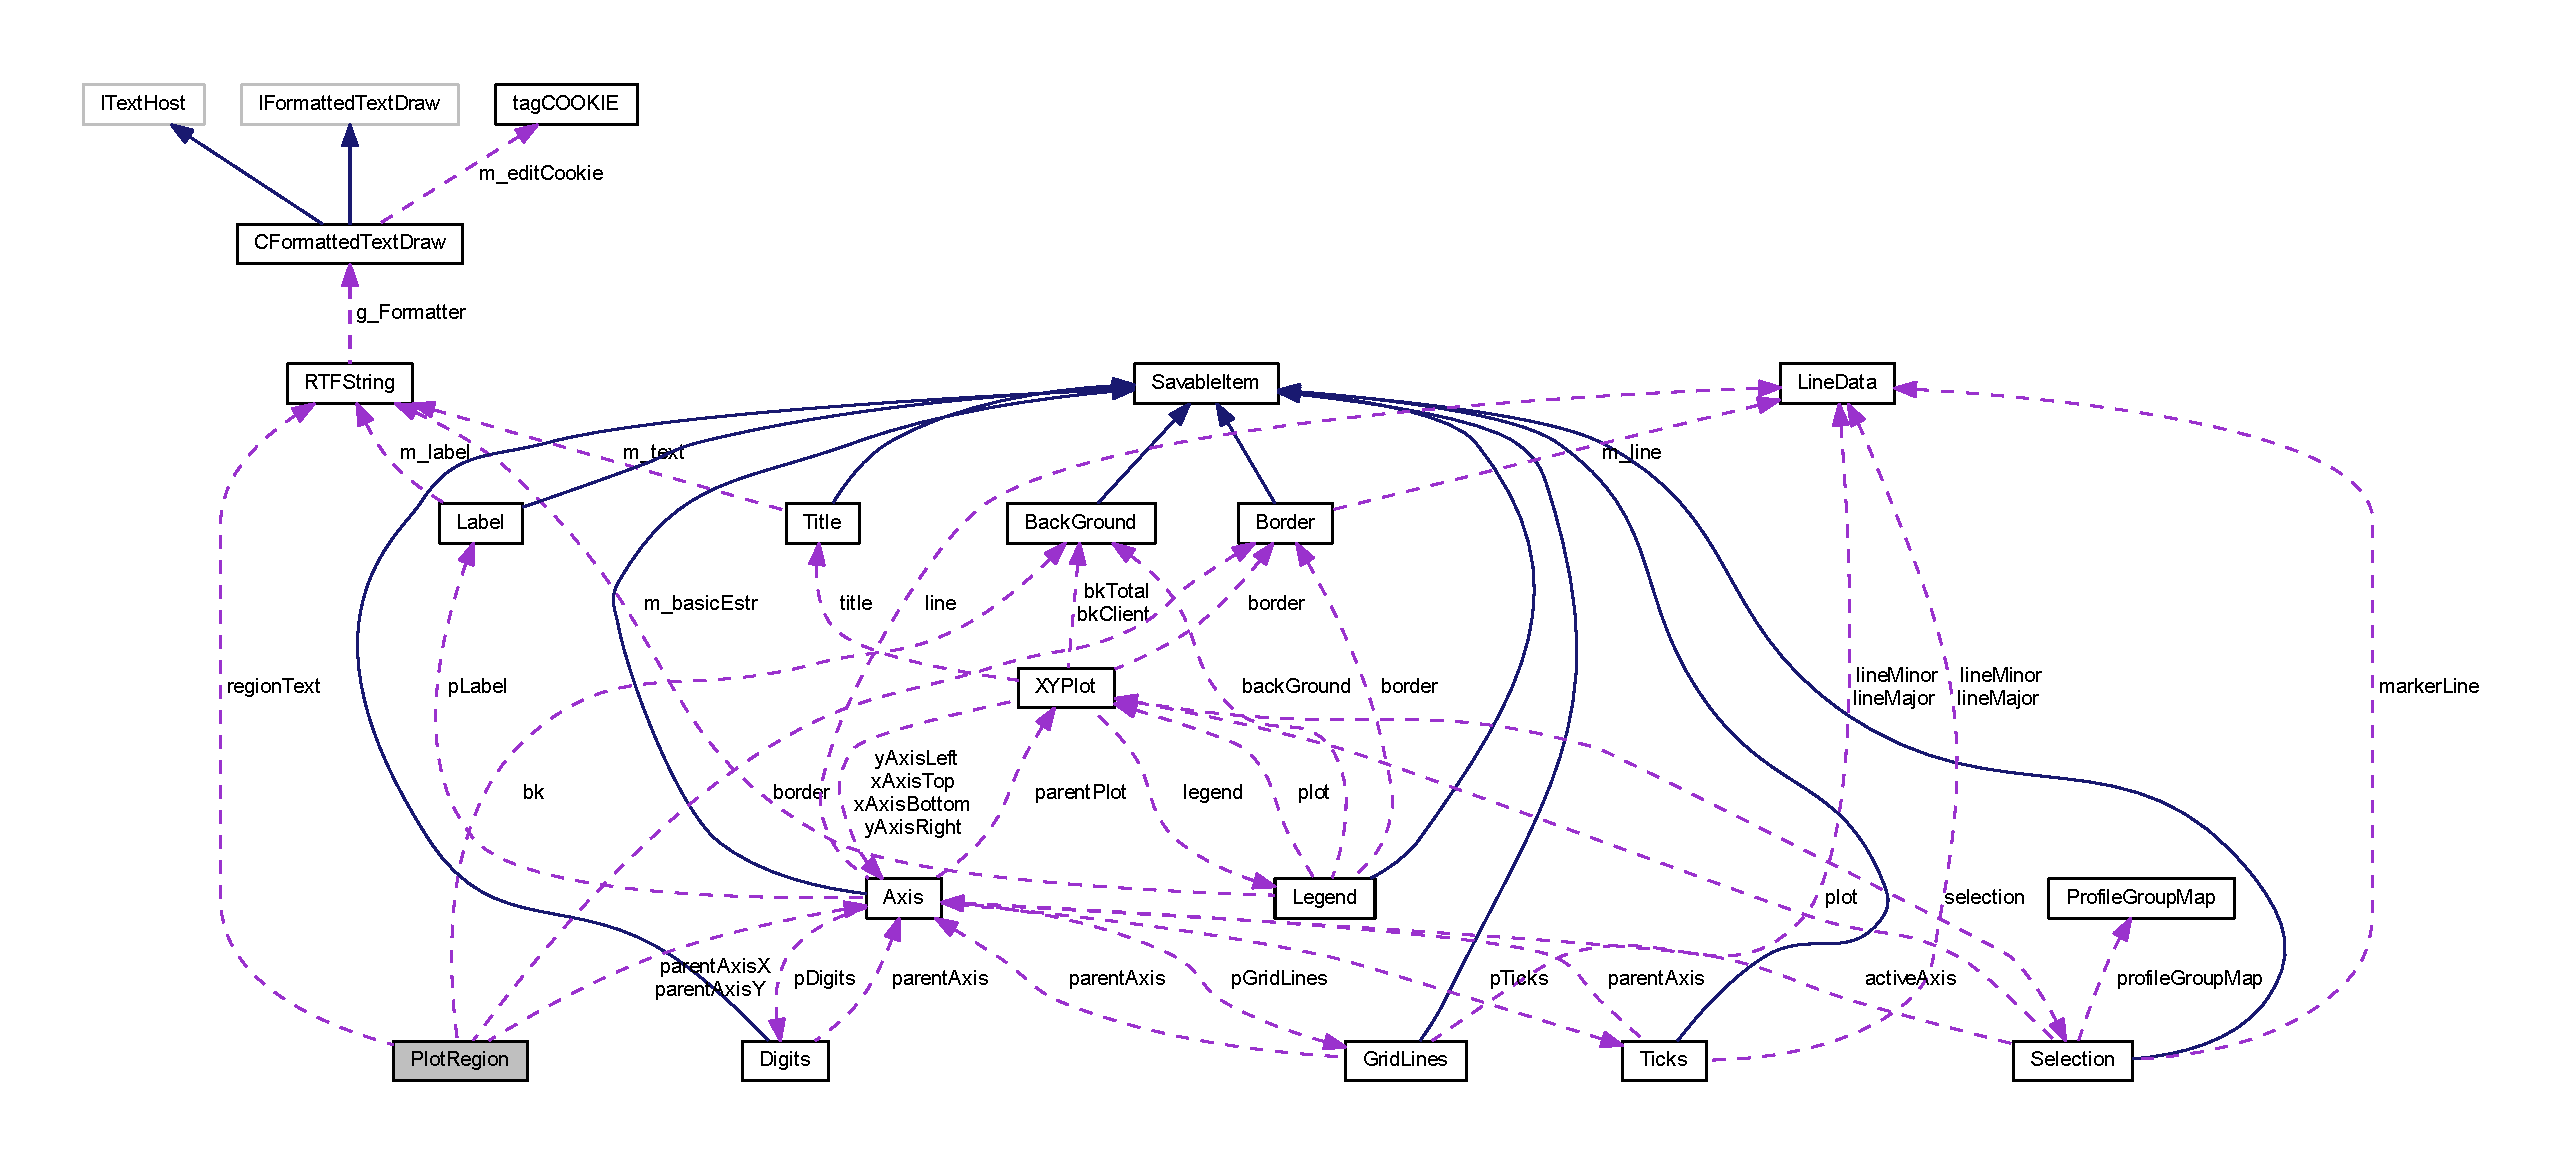
\includegraphics[width=350pt]{class_plot_region__coll__graph}
\end{center}
\end{figure}
\subsection*{Открытые члены}
\begin{DoxyCompactItemize}
\item 
\hyperlink{class_plot_region_aa20c4158814429875632d6d873a41aeb}{Plot\-Region} (\hyperlink{class_x_y_plot}{X\-Y\-Plot} $\ast$parent, \hyperlink{class_axis}{Axis} $\ast$axis\-X, \hyperlink{class_axis}{Axis} $\ast$axis\-Y, double pt\-From\-X, double pt\-From\-Y, double pt\-To\-X, double pt\-To\-Y, std\-::string label\-Text=\char`\"{}\char`\"{}, C\-O\-L\-O\-R\-R\-E\-F color=R\-G\-B(128, 80, 80), double opaque=100, C\-O\-L\-O\-R\-R\-E\-F Border\-Color=R\-G\-B(0, 0, 0), int Border\-Width=1, int Border\-Line=\hyperlink{namespacexyplot_a3d67107a3da8dc1ef0114ab0352e01eda50f3326c8ff8eb69d629156dfe2e268a}{xyplot\-::\-P\-L\-S\-\_\-\-S\-O\-L\-I\-D})
\item 
\hyperlink{class_plot_region_a30f37de224be906ff032def46b311d3c}{$\sim$\-Plot\-Region} (void)
\item 
B\-O\-O\-L \hyperlink{class_plot_region_a6a71fbeed8f2de90fe6e069a9b2e22c0}{Pre\-Draw} ()
\item 
void \hyperlink{class_plot_region_a508939830f7e43969b099c2836db5c4e}{On\-Draw} (H\-D\-C hdc)
\item 
void \hyperlink{class_plot_region_a8e8d84c8bca2c5badf833ec55e4ac089}{Set\-X\-Range} (double x1, double x2)
\item 
void \hyperlink{class_plot_region_a906d6cdb0f52224b37dc93fe5e3a2a98}{Set\-Y\-Range} (double y1, double y2)
\item 
C\-O\-L\-O\-R\-R\-E\-F \hyperlink{class_plot_region_a8c9115a80a42634d87a6ee1e95dd62d1}{Get\-Line\-Color} () const 
\item 
void \hyperlink{class_plot_region_aea5ce8db7c4e5ad0383b5bca8ceeceba}{Set\-Line\-Color} (C\-O\-L\-O\-R\-R\-E\-F color)
\item 
void \hyperlink{class_plot_region_aa627b45cacdbc50c3f6ae4cfbb66b75b}{Get\-Fill\-Colors} (C\-O\-L\-O\-R\-R\-E\-F \&clr\-Start, C\-O\-L\-O\-R\-R\-E\-F \&clr\-Finish) const 
\item 
void \hyperlink{class_plot_region_a7cb18f693dc5ca91e5220d753dcd710a}{Set\-Fill\-Colors} (C\-O\-L\-O\-R\-R\-E\-F clr\-Start, C\-O\-L\-O\-R\-R\-E\-F clr\-Finish)
\item 
void \hyperlink{class_plot_region_a973f741072a09ad701f31fd8cf8c7178}{Set\-Gradient\-Direction} (B\-O\-O\-L vertical)
\item 
B\-O\-O\-L \hyperlink{class_plot_region_a1a8c4048030e64ec3d29361363f6b3f3}{Get\-Gradient\-Direction} () const 
\item 
long \hyperlink{class_plot_region_a47b86ae228fae33d9448f8ac3c2a7c05}{Get\-Hatch\-Style} () const 
\item 
void \hyperlink{class_plot_region_afef080fb216a51c6a90f4b4ac8050ee2}{Set\-Hatch\-Style} (long hstyle)
\end{DoxyCompactItemize}
\subsection*{Защищенные данные}
\begin{DoxyCompactItemize}
\item 
const \hyperlink{class_axis}{Axis} \& \hyperlink{class_plot_region_aec00a997e0e41c233d8542a9ec4d602f}{parent\-Axis\-X}
\item 
const \hyperlink{class_axis}{Axis} \& \hyperlink{class_plot_region_ae817987187aded3ddb6074f1462f9b5c}{parent\-Axis\-Y}
\item 
\hyperlink{class_border}{Border} \hyperlink{class_plot_region_a66a8e6a2f04b30da9b84a618aeef17a2}{border}
\item 
\hyperlink{class_back_ground}{Back\-Ground} \hyperlink{class_plot_region_a73dfa8e41749b8f277264bd716f3621e}{bk}
\item 
R\-E\-C\-T \hyperlink{class_plot_region_ac277b90fffff8f74744646361e3c0887}{rgn\-Rect}
\item 
double \hyperlink{class_plot_region_a17c3a91a03edc979ef6fdd2fa317fc79}{x\-From}
\item 
double \hyperlink{class_plot_region_a8f988d5b4e0ae0995b4fe457b806064e}{x\-To}
\item 
double \hyperlink{class_plot_region_acf10bb3e21dc8efeadbc2ccd128a6772}{y\-From}
\item 
double \hyperlink{class_plot_region_ad97dd7a58a12907c939ad3d764ad0a7d}{y\-To}
\item 
C\-O\-L\-O\-R\-R\-E\-F \hyperlink{class_plot_region_a12dc144f3d93052dc1b2afd355b4372e}{hatch\-Color}
\item 
long \hyperlink{class_plot_region_a0a6bac6e99e972970b90e19aa1463fe6}{hatch\-Style}
\item 
\hyperlink{class_r_t_f_string}{R\-T\-F\-String} $\ast$ \hyperlink{class_plot_region_a76d55541c5f544224d99b3f44ee3c5ea}{region\-Text}
\end{DoxyCompactItemize}


\subsection{Конструктор(ы)}
\hypertarget{class_plot_region_aa20c4158814429875632d6d873a41aeb}{\index{Plot\-Region@{Plot\-Region}!Plot\-Region@{Plot\-Region}}
\index{Plot\-Region@{Plot\-Region}!PlotRegion@{Plot\-Region}}
\subsubsection[{Plot\-Region}]{\setlength{\rightskip}{0pt plus 5cm}Plot\-Region\-::\-Plot\-Region (
\begin{DoxyParamCaption}
\item[{{\bf X\-Y\-Plot} $\ast$}]{parent, }
\item[{{\bf Axis} $\ast$}]{axis\-X, }
\item[{{\bf Axis} $\ast$}]{axis\-Y, }
\item[{double}]{pt\-From\-X, }
\item[{double}]{pt\-From\-Y, }
\item[{double}]{pt\-To\-X, }
\item[{double}]{pt\-To\-Y, }
\item[{std\-::string}]{label\-Text = {\ttfamily \char`\"{}\char`\"{}}, }
\item[{C\-O\-L\-O\-R\-R\-E\-F}]{color = {\ttfamily RGB(128,80,80)}, }
\item[{double}]{opaque = {\ttfamily 100}, }
\item[{C\-O\-L\-O\-R\-R\-E\-F}]{Border\-Color = {\ttfamily RGB(0,0,0)}, }
\item[{int}]{Border\-Width = {\ttfamily 1}, }
\item[{int}]{Border\-Line = {\ttfamily {\bf xyplot\-::\-P\-L\-S\-\_\-\-S\-O\-L\-I\-D}}}
\end{DoxyParamCaption}
)}}\label{class_plot_region_aa20c4158814429875632d6d873a41aeb}
\hypertarget{class_plot_region_a30f37de224be906ff032def46b311d3c}{\index{Plot\-Region@{Plot\-Region}!$\sim$\-Plot\-Region@{$\sim$\-Plot\-Region}}
\index{$\sim$\-Plot\-Region@{$\sim$\-Plot\-Region}!PlotRegion@{Plot\-Region}}
\subsubsection[{$\sim$\-Plot\-Region}]{\setlength{\rightskip}{0pt plus 5cm}Plot\-Region\-::$\sim$\-Plot\-Region (
\begin{DoxyParamCaption}
\item[{void}]{}
\end{DoxyParamCaption}
)}}\label{class_plot_region_a30f37de224be906ff032def46b311d3c}


\subsection{Методы}
\hypertarget{class_plot_region_aa627b45cacdbc50c3f6ae4cfbb66b75b}{\index{Plot\-Region@{Plot\-Region}!Get\-Fill\-Colors@{Get\-Fill\-Colors}}
\index{Get\-Fill\-Colors@{Get\-Fill\-Colors}!PlotRegion@{Plot\-Region}}
\subsubsection[{Get\-Fill\-Colors}]{\setlength{\rightskip}{0pt plus 5cm}void Plot\-Region\-::\-Get\-Fill\-Colors (
\begin{DoxyParamCaption}
\item[{C\-O\-L\-O\-R\-R\-E\-F \&}]{clr\-Start, }
\item[{C\-O\-L\-O\-R\-R\-E\-F \&}]{clr\-Finish}
\end{DoxyParamCaption}
) const}}\label{class_plot_region_aa627b45cacdbc50c3f6ae4cfbb66b75b}
\hypertarget{class_plot_region_a1a8c4048030e64ec3d29361363f6b3f3}{\index{Plot\-Region@{Plot\-Region}!Get\-Gradient\-Direction@{Get\-Gradient\-Direction}}
\index{Get\-Gradient\-Direction@{Get\-Gradient\-Direction}!PlotRegion@{Plot\-Region}}
\subsubsection[{Get\-Gradient\-Direction}]{\setlength{\rightskip}{0pt plus 5cm}B\-O\-O\-L Plot\-Region\-::\-Get\-Gradient\-Direction (
\begin{DoxyParamCaption}
{}
\end{DoxyParamCaption}
) const}}\label{class_plot_region_a1a8c4048030e64ec3d29361363f6b3f3}
\hypertarget{class_plot_region_a47b86ae228fae33d9448f8ac3c2a7c05}{\index{Plot\-Region@{Plot\-Region}!Get\-Hatch\-Style@{Get\-Hatch\-Style}}
\index{Get\-Hatch\-Style@{Get\-Hatch\-Style}!PlotRegion@{Plot\-Region}}
\subsubsection[{Get\-Hatch\-Style}]{\setlength{\rightskip}{0pt plus 5cm}long Plot\-Region\-::\-Get\-Hatch\-Style (
\begin{DoxyParamCaption}
{}
\end{DoxyParamCaption}
) const}}\label{class_plot_region_a47b86ae228fae33d9448f8ac3c2a7c05}
\hypertarget{class_plot_region_a8c9115a80a42634d87a6ee1e95dd62d1}{\index{Plot\-Region@{Plot\-Region}!Get\-Line\-Color@{Get\-Line\-Color}}
\index{Get\-Line\-Color@{Get\-Line\-Color}!PlotRegion@{Plot\-Region}}
\subsubsection[{Get\-Line\-Color}]{\setlength{\rightskip}{0pt plus 5cm}C\-O\-L\-O\-R\-R\-E\-F Plot\-Region\-::\-Get\-Line\-Color (
\begin{DoxyParamCaption}
{}
\end{DoxyParamCaption}
) const}}\label{class_plot_region_a8c9115a80a42634d87a6ee1e95dd62d1}
\hypertarget{class_plot_region_a508939830f7e43969b099c2836db5c4e}{\index{Plot\-Region@{Plot\-Region}!On\-Draw@{On\-Draw}}
\index{On\-Draw@{On\-Draw}!PlotRegion@{Plot\-Region}}
\subsubsection[{On\-Draw}]{\setlength{\rightskip}{0pt plus 5cm}void Plot\-Region\-::\-On\-Draw (
\begin{DoxyParamCaption}
\item[{H\-D\-C}]{hdc}
\end{DoxyParamCaption}
)}}\label{class_plot_region_a508939830f7e43969b099c2836db5c4e}
\hypertarget{class_plot_region_a6a71fbeed8f2de90fe6e069a9b2e22c0}{\index{Plot\-Region@{Plot\-Region}!Pre\-Draw@{Pre\-Draw}}
\index{Pre\-Draw@{Pre\-Draw}!PlotRegion@{Plot\-Region}}
\subsubsection[{Pre\-Draw}]{\setlength{\rightskip}{0pt plus 5cm}B\-O\-O\-L Plot\-Region\-::\-Pre\-Draw (
\begin{DoxyParamCaption}
{}
\end{DoxyParamCaption}
)}}\label{class_plot_region_a6a71fbeed8f2de90fe6e069a9b2e22c0}
\hypertarget{class_plot_region_a7cb18f693dc5ca91e5220d753dcd710a}{\index{Plot\-Region@{Plot\-Region}!Set\-Fill\-Colors@{Set\-Fill\-Colors}}
\index{Set\-Fill\-Colors@{Set\-Fill\-Colors}!PlotRegion@{Plot\-Region}}
\subsubsection[{Set\-Fill\-Colors}]{\setlength{\rightskip}{0pt plus 5cm}void Plot\-Region\-::\-Set\-Fill\-Colors (
\begin{DoxyParamCaption}
\item[{C\-O\-L\-O\-R\-R\-E\-F}]{clr\-Start, }
\item[{C\-O\-L\-O\-R\-R\-E\-F}]{clr\-Finish}
\end{DoxyParamCaption}
)}}\label{class_plot_region_a7cb18f693dc5ca91e5220d753dcd710a}
\hypertarget{class_plot_region_a973f741072a09ad701f31fd8cf8c7178}{\index{Plot\-Region@{Plot\-Region}!Set\-Gradient\-Direction@{Set\-Gradient\-Direction}}
\index{Set\-Gradient\-Direction@{Set\-Gradient\-Direction}!PlotRegion@{Plot\-Region}}
\subsubsection[{Set\-Gradient\-Direction}]{\setlength{\rightskip}{0pt plus 5cm}void Plot\-Region\-::\-Set\-Gradient\-Direction (
\begin{DoxyParamCaption}
\item[{B\-O\-O\-L}]{vertical}
\end{DoxyParamCaption}
)}}\label{class_plot_region_a973f741072a09ad701f31fd8cf8c7178}
\hypertarget{class_plot_region_afef080fb216a51c6a90f4b4ac8050ee2}{\index{Plot\-Region@{Plot\-Region}!Set\-Hatch\-Style@{Set\-Hatch\-Style}}
\index{Set\-Hatch\-Style@{Set\-Hatch\-Style}!PlotRegion@{Plot\-Region}}
\subsubsection[{Set\-Hatch\-Style}]{\setlength{\rightskip}{0pt plus 5cm}void Plot\-Region\-::\-Set\-Hatch\-Style (
\begin{DoxyParamCaption}
\item[{long}]{hstyle}
\end{DoxyParamCaption}
)}}\label{class_plot_region_afef080fb216a51c6a90f4b4ac8050ee2}
\hypertarget{class_plot_region_aea5ce8db7c4e5ad0383b5bca8ceeceba}{\index{Plot\-Region@{Plot\-Region}!Set\-Line\-Color@{Set\-Line\-Color}}
\index{Set\-Line\-Color@{Set\-Line\-Color}!PlotRegion@{Plot\-Region}}
\subsubsection[{Set\-Line\-Color}]{\setlength{\rightskip}{0pt plus 5cm}void Plot\-Region\-::\-Set\-Line\-Color (
\begin{DoxyParamCaption}
\item[{C\-O\-L\-O\-R\-R\-E\-F}]{color}
\end{DoxyParamCaption}
)}}\label{class_plot_region_aea5ce8db7c4e5ad0383b5bca8ceeceba}
\hypertarget{class_plot_region_a8e8d84c8bca2c5badf833ec55e4ac089}{\index{Plot\-Region@{Plot\-Region}!Set\-X\-Range@{Set\-X\-Range}}
\index{Set\-X\-Range@{Set\-X\-Range}!PlotRegion@{Plot\-Region}}
\subsubsection[{Set\-X\-Range}]{\setlength{\rightskip}{0pt plus 5cm}void Plot\-Region\-::\-Set\-X\-Range (
\begin{DoxyParamCaption}
\item[{double}]{x1, }
\item[{double}]{x2}
\end{DoxyParamCaption}
)}}\label{class_plot_region_a8e8d84c8bca2c5badf833ec55e4ac089}
\hypertarget{class_plot_region_a906d6cdb0f52224b37dc93fe5e3a2a98}{\index{Plot\-Region@{Plot\-Region}!Set\-Y\-Range@{Set\-Y\-Range}}
\index{Set\-Y\-Range@{Set\-Y\-Range}!PlotRegion@{Plot\-Region}}
\subsubsection[{Set\-Y\-Range}]{\setlength{\rightskip}{0pt plus 5cm}void Plot\-Region\-::\-Set\-Y\-Range (
\begin{DoxyParamCaption}
\item[{double}]{y1, }
\item[{double}]{y2}
\end{DoxyParamCaption}
)}}\label{class_plot_region_a906d6cdb0f52224b37dc93fe5e3a2a98}


\subsection{Данные класса}
\hypertarget{class_plot_region_a73dfa8e41749b8f277264bd716f3621e}{\index{Plot\-Region@{Plot\-Region}!bk@{bk}}
\index{bk@{bk}!PlotRegion@{Plot\-Region}}
\subsubsection[{bk}]{\setlength{\rightskip}{0pt plus 5cm}{\bf Back\-Ground} Plot\-Region\-::bk\hspace{0.3cm}{\ttfamily [protected]}}}\label{class_plot_region_a73dfa8e41749b8f277264bd716f3621e}
\hypertarget{class_plot_region_a66a8e6a2f04b30da9b84a618aeef17a2}{\index{Plot\-Region@{Plot\-Region}!border@{border}}
\index{border@{border}!PlotRegion@{Plot\-Region}}
\subsubsection[{border}]{\setlength{\rightskip}{0pt plus 5cm}{\bf Border} Plot\-Region\-::border\hspace{0.3cm}{\ttfamily [protected]}}}\label{class_plot_region_a66a8e6a2f04b30da9b84a618aeef17a2}
\hypertarget{class_plot_region_a12dc144f3d93052dc1b2afd355b4372e}{\index{Plot\-Region@{Plot\-Region}!hatch\-Color@{hatch\-Color}}
\index{hatch\-Color@{hatch\-Color}!PlotRegion@{Plot\-Region}}
\subsubsection[{hatch\-Color}]{\setlength{\rightskip}{0pt plus 5cm}C\-O\-L\-O\-R\-R\-E\-F Plot\-Region\-::hatch\-Color\hspace{0.3cm}{\ttfamily [protected]}}}\label{class_plot_region_a12dc144f3d93052dc1b2afd355b4372e}
\hypertarget{class_plot_region_a0a6bac6e99e972970b90e19aa1463fe6}{\index{Plot\-Region@{Plot\-Region}!hatch\-Style@{hatch\-Style}}
\index{hatch\-Style@{hatch\-Style}!PlotRegion@{Plot\-Region}}
\subsubsection[{hatch\-Style}]{\setlength{\rightskip}{0pt plus 5cm}long Plot\-Region\-::hatch\-Style\hspace{0.3cm}{\ttfamily [protected]}}}\label{class_plot_region_a0a6bac6e99e972970b90e19aa1463fe6}
\hypertarget{class_plot_region_aec00a997e0e41c233d8542a9ec4d602f}{\index{Plot\-Region@{Plot\-Region}!parent\-Axis\-X@{parent\-Axis\-X}}
\index{parent\-Axis\-X@{parent\-Axis\-X}!PlotRegion@{Plot\-Region}}
\subsubsection[{parent\-Axis\-X}]{\setlength{\rightskip}{0pt plus 5cm}const {\bf Axis}\& Plot\-Region\-::parent\-Axis\-X\hspace{0.3cm}{\ttfamily [protected]}}}\label{class_plot_region_aec00a997e0e41c233d8542a9ec4d602f}
\hypertarget{class_plot_region_ae817987187aded3ddb6074f1462f9b5c}{\index{Plot\-Region@{Plot\-Region}!parent\-Axis\-Y@{parent\-Axis\-Y}}
\index{parent\-Axis\-Y@{parent\-Axis\-Y}!PlotRegion@{Plot\-Region}}
\subsubsection[{parent\-Axis\-Y}]{\setlength{\rightskip}{0pt plus 5cm}const {\bf Axis}\& Plot\-Region\-::parent\-Axis\-Y\hspace{0.3cm}{\ttfamily [protected]}}}\label{class_plot_region_ae817987187aded3ddb6074f1462f9b5c}
\hypertarget{class_plot_region_a76d55541c5f544224d99b3f44ee3c5ea}{\index{Plot\-Region@{Plot\-Region}!region\-Text@{region\-Text}}
\index{region\-Text@{region\-Text}!PlotRegion@{Plot\-Region}}
\subsubsection[{region\-Text}]{\setlength{\rightskip}{0pt plus 5cm}{\bf R\-T\-F\-String}$\ast$ Plot\-Region\-::region\-Text\hspace{0.3cm}{\ttfamily [protected]}}}\label{class_plot_region_a76d55541c5f544224d99b3f44ee3c5ea}
\hypertarget{class_plot_region_ac277b90fffff8f74744646361e3c0887}{\index{Plot\-Region@{Plot\-Region}!rgn\-Rect@{rgn\-Rect}}
\index{rgn\-Rect@{rgn\-Rect}!PlotRegion@{Plot\-Region}}
\subsubsection[{rgn\-Rect}]{\setlength{\rightskip}{0pt plus 5cm}R\-E\-C\-T Plot\-Region\-::rgn\-Rect\hspace{0.3cm}{\ttfamily [protected]}}}\label{class_plot_region_ac277b90fffff8f74744646361e3c0887}
\hypertarget{class_plot_region_a17c3a91a03edc979ef6fdd2fa317fc79}{\index{Plot\-Region@{Plot\-Region}!x\-From@{x\-From}}
\index{x\-From@{x\-From}!PlotRegion@{Plot\-Region}}
\subsubsection[{x\-From}]{\setlength{\rightskip}{0pt plus 5cm}double Plot\-Region\-::x\-From\hspace{0.3cm}{\ttfamily [protected]}}}\label{class_plot_region_a17c3a91a03edc979ef6fdd2fa317fc79}
\hypertarget{class_plot_region_a8f988d5b4e0ae0995b4fe457b806064e}{\index{Plot\-Region@{Plot\-Region}!x\-To@{x\-To}}
\index{x\-To@{x\-To}!PlotRegion@{Plot\-Region}}
\subsubsection[{x\-To}]{\setlength{\rightskip}{0pt plus 5cm}double Plot\-Region\-::x\-To\hspace{0.3cm}{\ttfamily [protected]}}}\label{class_plot_region_a8f988d5b4e0ae0995b4fe457b806064e}
\hypertarget{class_plot_region_acf10bb3e21dc8efeadbc2ccd128a6772}{\index{Plot\-Region@{Plot\-Region}!y\-From@{y\-From}}
\index{y\-From@{y\-From}!PlotRegion@{Plot\-Region}}
\subsubsection[{y\-From}]{\setlength{\rightskip}{0pt plus 5cm}double Plot\-Region\-::y\-From\hspace{0.3cm}{\ttfamily [protected]}}}\label{class_plot_region_acf10bb3e21dc8efeadbc2ccd128a6772}
\hypertarget{class_plot_region_ad97dd7a58a12907c939ad3d764ad0a7d}{\index{Plot\-Region@{Plot\-Region}!y\-To@{y\-To}}
\index{y\-To@{y\-To}!PlotRegion@{Plot\-Region}}
\subsubsection[{y\-To}]{\setlength{\rightskip}{0pt plus 5cm}double Plot\-Region\-::y\-To\hspace{0.3cm}{\ttfamily [protected]}}}\label{class_plot_region_ad97dd7a58a12907c939ad3d764ad0a7d}


Объявления и описания членов классов находятся в файлах\-:\begin{DoxyCompactItemize}
\item 
src/\hyperlink{_regions_8h}{Regions.\-h}\item 
src/\hyperlink{_regions_8cpp}{Regions.\-cpp}\end{DoxyCompactItemize}

\hypertarget{class_profile}{\section{Класс Profile}
\label{class_profile}\index{Profile@{Profile}}
}


{\ttfamily \#include $<$profile.\-h$>$}



Граф связей класса Profile\-:
\nopagebreak
\begin{figure}[H]
\begin{center}
\leavevmode
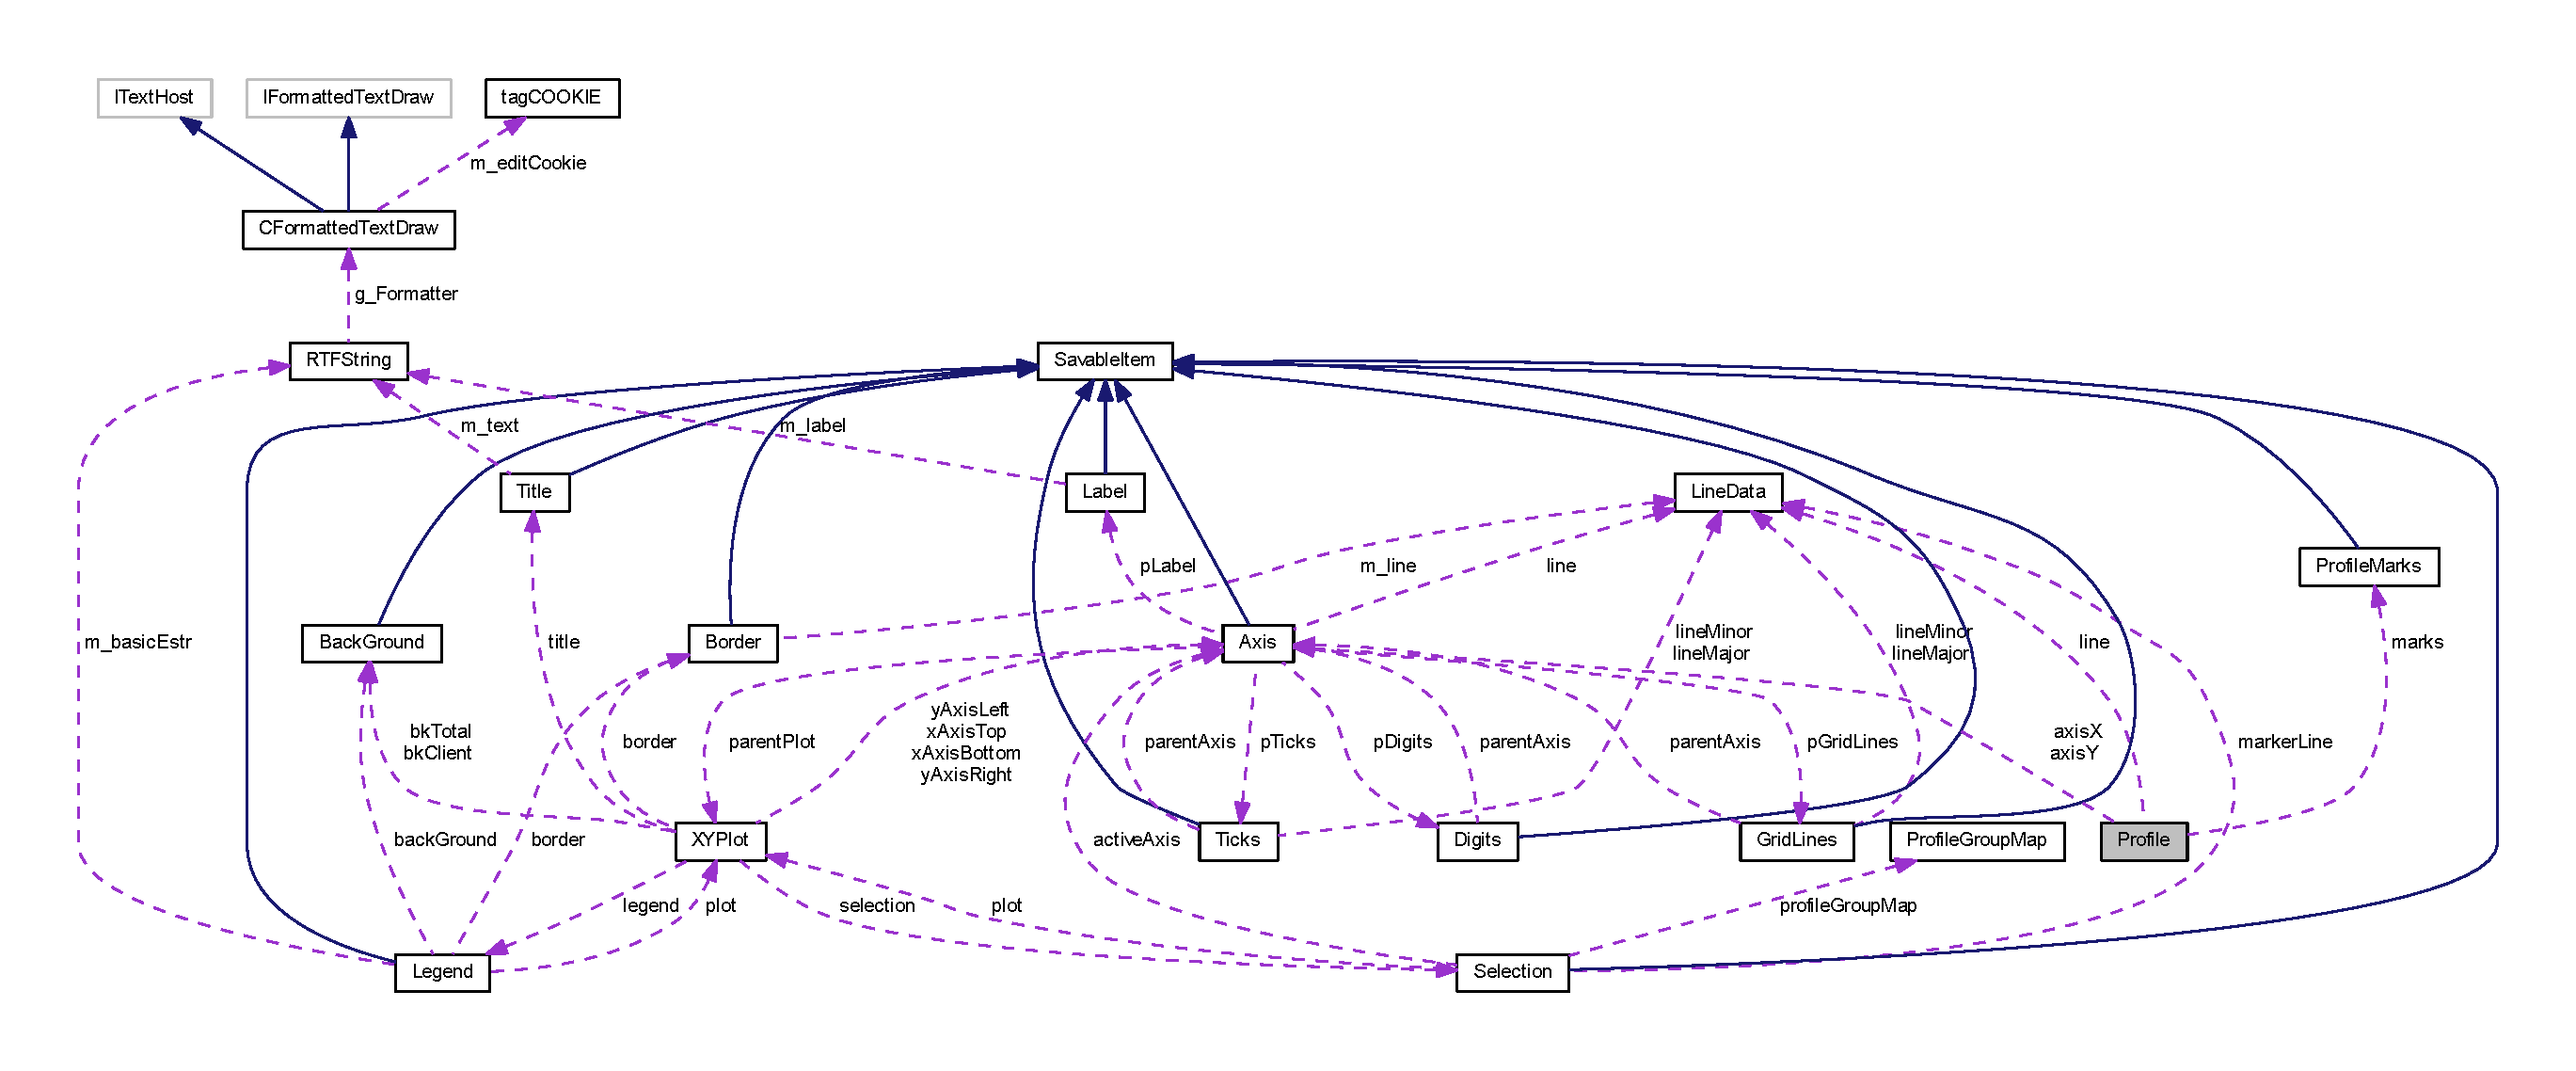
\includegraphics[width=350pt]{class_profile__coll__graph}
\end{center}
\end{figure}
\subsection*{Открытые члены}
\begin{DoxyCompactItemize}
\item 
\hyperlink{class_profile_a0af304ee61478092d010df5dc146bd06}{Profile} (std\-::string \hyperlink{class_profile_ac8a75db2da9448616fb180edcc25bf8c}{name}, long color, int width, B\-O\-O\-L \hyperlink{class_profile_a7e12899117a7229fd74e727d4c7508aa}{show\-Line}, B\-O\-O\-L \hyperlink{class_profile_a07364e07ee0c925c0b2a7631c666056b}{show\-Marks}, const \hyperlink{class_axis}{Axis} \&\hyperlink{class_profile_a9ab5958c5e36ddb1c8dc96773bfbaeb6}{axis\-X}, const \hyperlink{class_axis}{Axis} \&\hyperlink{class_profile_af934163fd90437181ce2125860214cd0}{axis\-Y})
\item 
\hyperlink{class_profile_a58fa758a59bc4ee3c1a9980e360e4e98}{$\sim$\-Profile} ()
\item 
void \hyperlink{class_profile_af982d6eea235d68ebd74f102ef29d12a}{Set\-Name} (std\-::string \hyperlink{class_profile_ac8a75db2da9448616fb180edcc25bf8c}{name})
\item 
const std\-::string \& \hyperlink{class_profile_aa6baeea130f07d7027117d1663619251}{Get\-Name} () const 
\item 
void \hyperlink{class_profile_a6ae3bac4830d7b81cfc5daefeb406445}{Set\-Visible} (B\-O\-O\-L visible=T\-R\-U\-E)
\item 
B\-O\-O\-L \hyperlink{class_profile_a381fe66a6e251a351c0157587d609ad7}{Is\-Visible} () const 
\item 
void \hyperlink{class_profile_a839300e94f6e588988c5b25e167de9dd}{Use\-Symblos} (B\-O\-O\-L symblols)
\item 
B\-O\-O\-L \hyperlink{class_profile_a431d9a16e08188d7ad014c0d20696237}{Is\-Use\-Symblos} () const 
\item 
void \hyperlink{class_profile_a2f9a7420f40b1cc4974a2fe6b1a2aca8}{Show} (B\-O\-O\-L b\-Show)
\item 
long \hyperlink{class_profile_aacee6e0f579d0dbcc6f8452778907473}{Get\-Unit} (unsigned index, double \&x, double \&y) const 
\item 
long \hyperlink{class_profile_a844b59dcfb67d36f70f322425b7f98ee}{Get\-Data} (unsigned $\ast$count, double $\ast$pfx, double $\ast$pfy) const 
\item 
void \hyperlink{class_profile_aa272424c24ba0eacdd3aa725c6e44e98}{Set\-Data} (const double $\ast$pfx, const double $\ast$pfy, int count)
\item 
B\-O\-O\-L \hyperlink{class_profile_abf535c50bda946ff73128a5d686d0d36}{Empty} () const 
\item 
void \hyperlink{class_profile_a5c65fe41c9872b365adec25e5dc0376d}{Append} (double fx, double fy)
\item 
void \hyperlink{class_profile_a8aede9dc40d7161d8e4f5e8e49a1894f}{Append} (const double $\ast$pfx, const double $\ast$pfy, unsigned count)
\item 
unsigned \hyperlink{class_profile_ac99b05caf969d1100a096872896decff}{Data\-Size} () const 
\item 
void \hyperlink{class_profile_a71927cb9bcbbe8a02947ffc25afdadd9}{Set\-Line\-Data} (const \hyperlink{class_line_data}{Line\-Data} \&src\-Line)
\item 
\hyperlink{class_line_data}{Line\-Data} \& \hyperlink{class_profile_a476640b07ed944d59dc55efe64fe15c7}{Get\-Line\-Data} ()
\item 
void \hyperlink{class_profile_a2bdae58cd0a58abcd2a7e51368a693b1}{Range} (double \&xmin, double \&xmax, double \&ymin, double \&ymax) const 
\item 
void \hyperlink{class_profile_ac0d79d6f6b2355fe6e13262319968368}{Range\-X} (double \&xmin, double \&xmax) const 
\item 
void \hyperlink{class_profile_af838a64a6376e9f083a621edd4604777}{Range\-Y} (double \&xmin, double \&xmax) const 
\item 
void \hyperlink{class_profile_a2d8f93d7a343455f9b8168220d1880d2}{Render} (H\-D\-C h\-D\-C, const R\-E\-C\-T rect)
\item 
const P\-O\-I\-N\-T $\ast$ \hyperlink{class_profile_af82006b877d02e4f5f725118f95fa59e}{Get\-Render\-Point\-Array} (unsigned \&count) const 
\item 
const P\-O\-I\-N\-T \hyperlink{class_profile_a83e9c9f23f67511b0bbd3aec4c256821}{Get\-Render\-Point} (int index, double \&phys\-X, double \&phys\-Y) const 
\item 
\hyperlink{class_profile_marks}{Profile\-Marks} \& \hyperlink{class_profile_ad11605c10819b4d259474ddc0a888334}{Get\-Marks} ()
\item 
\hyperlink{class_axis}{Axis} \& \hyperlink{class_profile_a0faa93dd60b346e486b2c1a084c05836}{Axis\-X} ()
\item 
\hyperlink{class_axis}{Axis} \& \hyperlink{class_profile_af891a7ad2f1f7508822c41e542e0edf2}{Axis\-Y} ()
\item 
B\-O\-O\-L \hyperlink{class_profile_a48a263ac82a825c8c0208bbb2532e5d9}{Is\-Show\-In\-Legend} () const 
\item 
void \hyperlink{class_profile_a69bc4295a958de5f72aa67ab70b3d036}{Show\-In\-Legend} (B\-O\-O\-L show)
\item 
void \hyperlink{class_profile_ac8069bd46802baa2c0fa53419425b159}{Get\-Visible\-Range} (unsigned \&first\-Index, unsigned \&last\-Index) const 
\end{DoxyCompactItemize}
\subsection*{Статические открытые данные}
\begin{DoxyCompactItemize}
\item 
static const int \hyperlink{class_profile_adc5551c9cef4089bd32d5358c2d27ec5}{D\-E\-F\-A\-U\-L\-T\-W\-I\-D\-T\-H} = 2
\end{DoxyCompactItemize}
\subsection*{Защищенные члены}
\begin{DoxyCompactItemize}
\item 
void \hyperlink{class_profile_a3cd865158aed8a6335c132acec3b734f}{Reset} ()
\end{DoxyCompactItemize}
\subsection*{Защищенные данные}
\begin{DoxyCompactItemize}
\item 
std\-::string \hyperlink{class_profile_ac8a75db2da9448616fb180edcc25bf8c}{name}
\item 
B\-O\-O\-L \hyperlink{class_profile_a07364e07ee0c925c0b2a7631c666056b}{show\-Marks}
\item 
B\-O\-O\-L \hyperlink{class_profile_a7e12899117a7229fd74e727d4c7508aa}{show\-Line}
\item 
\hyperlink{class_line_data}{Line\-Data} \hyperlink{class_profile_a63eba30a8236070b9ed979e1ebdd8709}{line}
\item 
\hyperlink{class_axis}{Axis} \& \hyperlink{class_profile_a9ab5958c5e36ddb1c8dc96773bfbaeb6}{axis\-X}
\item 
\hyperlink{class_axis}{Axis} \& \hyperlink{class_profile_af934163fd90437181ce2125860214cd0}{axis\-Y}
\item 
B\-O\-O\-L \hyperlink{class_profile_a2a37b4d72a0c1dcefcf65aa6474d8ca3}{new\-Data}
\item 
R\-E\-C\-T \hyperlink{class_profile_a21fbb7028f71f681ad6becd412f34e07}{last\-Rendered\-Rect}
\item 
double \hyperlink{class_profile_a7ec1de15af31223a7cba55fb711ce2c5}{min\-X}
\item 
double \hyperlink{class_profile_a3d4ffb95639a391469dc7f5b97fba63b}{max\-X}
\item 
double \hyperlink{class_profile_ab65307e12c8d002effb1de3598d47e00}{min\-Y}
\item 
double \hyperlink{class_profile_ac16836105d7961c71046014887d3cb71}{max\-Y}
\item 
\hyperlink{class_profile_marks}{Profile\-Marks} \hyperlink{class_profile_afb294101d0593f41db3f20fb1e678906}{marks}
\item 
std\-::vector$<$ P\-O\-I\-N\-T $>$ \hyperlink{class_profile_a7143abb96dc0d5ef1b152d1ce0ee8dac}{data\-Device}
\item 
std\-::vector$<$ double $>$ \hyperlink{class_profile_a9b8d3156a467dc594b39ee8224b659c3}{data\-Phys\-X}
\item 
std\-::vector$<$ double $>$ \hyperlink{class_profile_acb59691aee18d478753d4aedfafc8787}{data\-Phys\-Y}
\item 
B\-O\-O\-L \hyperlink{class_profile_a09c7baa3c0a3b1762f8c0eed5223868f}{show\-In\-Legend}
\item 
unsigned \hyperlink{class_profile_a877766d4f4ee2eb4f63220ebbbcf2e69}{first\-Visible}
\item 
unsigned \hyperlink{class_profile_ad48970e92143859da4f950c1c8fee217}{last\-Visible}
\item 
C\-R\-I\-T\-I\-C\-A\-L\-\_\-\-S\-E\-C\-T\-I\-O\-N \hyperlink{class_profile_a11aa9c768f5ff249dda920c04b886cd9}{cs}
\end{DoxyCompactItemize}


\subsection{Конструктор(ы)}
\hypertarget{class_profile_a0af304ee61478092d010df5dc146bd06}{\index{Profile@{Profile}!Profile@{Profile}}
\index{Profile@{Profile}!Profile@{Profile}}
\subsubsection[{Profile}]{\setlength{\rightskip}{0pt plus 5cm}Profile\-::\-Profile (
\begin{DoxyParamCaption}
\item[{std\-::string}]{name, }
\item[{long}]{color, }
\item[{int}]{width, }
\item[{B\-O\-O\-L}]{show\-Line, }
\item[{B\-O\-O\-L}]{show\-Marks, }
\item[{const {\bf Axis} \&}]{axis\-X, }
\item[{const {\bf Axis} \&}]{axis\-Y}
\end{DoxyParamCaption}
)}}\label{class_profile_a0af304ee61478092d010df5dc146bd06}
\hypertarget{class_profile_a58fa758a59bc4ee3c1a9980e360e4e98}{\index{Profile@{Profile}!$\sim$\-Profile@{$\sim$\-Profile}}
\index{$\sim$\-Profile@{$\sim$\-Profile}!Profile@{Profile}}
\subsubsection[{$\sim$\-Profile}]{\setlength{\rightskip}{0pt plus 5cm}Profile\-::$\sim$\-Profile (
\begin{DoxyParamCaption}
{}
\end{DoxyParamCaption}
)}}\label{class_profile_a58fa758a59bc4ee3c1a9980e360e4e98}


\subsection{Методы}
\hypertarget{class_profile_a5c65fe41c9872b365adec25e5dc0376d}{\index{Profile@{Profile}!Append@{Append}}
\index{Append@{Append}!Profile@{Profile}}
\subsubsection[{Append}]{\setlength{\rightskip}{0pt plus 5cm}void Profile\-::\-Append (
\begin{DoxyParamCaption}
\item[{double}]{fx, }
\item[{double}]{fy}
\end{DoxyParamCaption}
)}}\label{class_profile_a5c65fe41c9872b365adec25e5dc0376d}
\hypertarget{class_profile_a8aede9dc40d7161d8e4f5e8e49a1894f}{\index{Profile@{Profile}!Append@{Append}}
\index{Append@{Append}!Profile@{Profile}}
\subsubsection[{Append}]{\setlength{\rightskip}{0pt plus 5cm}void Profile\-::\-Append (
\begin{DoxyParamCaption}
\item[{const double $\ast$}]{pfx, }
\item[{const double $\ast$}]{pfy, }
\item[{unsigned}]{count}
\end{DoxyParamCaption}
)}}\label{class_profile_a8aede9dc40d7161d8e4f5e8e49a1894f}
\hypertarget{class_profile_a0faa93dd60b346e486b2c1a084c05836}{\index{Profile@{Profile}!Axis\-X@{Axis\-X}}
\index{Axis\-X@{Axis\-X}!Profile@{Profile}}
\subsubsection[{Axis\-X}]{\setlength{\rightskip}{0pt plus 5cm}{\bf Axis}\& Profile\-::\-Axis\-X (
\begin{DoxyParamCaption}
{}
\end{DoxyParamCaption}
)\hspace{0.3cm}{\ttfamily [inline]}}}\label{class_profile_a0faa93dd60b346e486b2c1a084c05836}
\hypertarget{class_profile_af891a7ad2f1f7508822c41e542e0edf2}{\index{Profile@{Profile}!Axis\-Y@{Axis\-Y}}
\index{Axis\-Y@{Axis\-Y}!Profile@{Profile}}
\subsubsection[{Axis\-Y}]{\setlength{\rightskip}{0pt plus 5cm}{\bf Axis}\& Profile\-::\-Axis\-Y (
\begin{DoxyParamCaption}
{}
\end{DoxyParamCaption}
)\hspace{0.3cm}{\ttfamily [inline]}}}\label{class_profile_af891a7ad2f1f7508822c41e542e0edf2}
\hypertarget{class_profile_ac99b05caf969d1100a096872896decff}{\index{Profile@{Profile}!Data\-Size@{Data\-Size}}
\index{Data\-Size@{Data\-Size}!Profile@{Profile}}
\subsubsection[{Data\-Size}]{\setlength{\rightskip}{0pt plus 5cm}unsigned Profile\-::\-Data\-Size (
\begin{DoxyParamCaption}
{}
\end{DoxyParamCaption}
) const\hspace{0.3cm}{\ttfamily [inline]}}}\label{class_profile_ac99b05caf969d1100a096872896decff}
\hypertarget{class_profile_abf535c50bda946ff73128a5d686d0d36}{\index{Profile@{Profile}!Empty@{Empty}}
\index{Empty@{Empty}!Profile@{Profile}}
\subsubsection[{Empty}]{\setlength{\rightskip}{0pt plus 5cm}B\-O\-O\-L Profile\-::\-Empty (
\begin{DoxyParamCaption}
{}
\end{DoxyParamCaption}
) const\hspace{0.3cm}{\ttfamily [inline]}}}\label{class_profile_abf535c50bda946ff73128a5d686d0d36}
\hypertarget{class_profile_a844b59dcfb67d36f70f322425b7f98ee}{\index{Profile@{Profile}!Get\-Data@{Get\-Data}}
\index{Get\-Data@{Get\-Data}!Profile@{Profile}}
\subsubsection[{Get\-Data}]{\setlength{\rightskip}{0pt plus 5cm}long Profile\-::\-Get\-Data (
\begin{DoxyParamCaption}
\item[{unsigned $\ast$}]{count, }
\item[{double $\ast$}]{pfx, }
\item[{double $\ast$}]{pfy}
\end{DoxyParamCaption}
) const}}\label{class_profile_a844b59dcfb67d36f70f322425b7f98ee}
\hypertarget{class_profile_a476640b07ed944d59dc55efe64fe15c7}{\index{Profile@{Profile}!Get\-Line\-Data@{Get\-Line\-Data}}
\index{Get\-Line\-Data@{Get\-Line\-Data}!Profile@{Profile}}
\subsubsection[{Get\-Line\-Data}]{\setlength{\rightskip}{0pt plus 5cm}{\bf Line\-Data}\& Profile\-::\-Get\-Line\-Data (
\begin{DoxyParamCaption}
{}
\end{DoxyParamCaption}
)\hspace{0.3cm}{\ttfamily [inline]}}}\label{class_profile_a476640b07ed944d59dc55efe64fe15c7}
\hypertarget{class_profile_ad11605c10819b4d259474ddc0a888334}{\index{Profile@{Profile}!Get\-Marks@{Get\-Marks}}
\index{Get\-Marks@{Get\-Marks}!Profile@{Profile}}
\subsubsection[{Get\-Marks}]{\setlength{\rightskip}{0pt plus 5cm}{\bf Profile\-Marks}\& Profile\-::\-Get\-Marks (
\begin{DoxyParamCaption}
{}
\end{DoxyParamCaption}
)\hspace{0.3cm}{\ttfamily [inline]}}}\label{class_profile_ad11605c10819b4d259474ddc0a888334}
\hypertarget{class_profile_aa6baeea130f07d7027117d1663619251}{\index{Profile@{Profile}!Get\-Name@{Get\-Name}}
\index{Get\-Name@{Get\-Name}!Profile@{Profile}}
\subsubsection[{Get\-Name}]{\setlength{\rightskip}{0pt plus 5cm}const std\-::string\& Profile\-::\-Get\-Name (
\begin{DoxyParamCaption}
{}
\end{DoxyParamCaption}
) const\hspace{0.3cm}{\ttfamily [inline]}}}\label{class_profile_aa6baeea130f07d7027117d1663619251}
\hypertarget{class_profile_a83e9c9f23f67511b0bbd3aec4c256821}{\index{Profile@{Profile}!Get\-Render\-Point@{Get\-Render\-Point}}
\index{Get\-Render\-Point@{Get\-Render\-Point}!Profile@{Profile}}
\subsubsection[{Get\-Render\-Point}]{\setlength{\rightskip}{0pt plus 5cm}const P\-O\-I\-N\-T Profile\-::\-Get\-Render\-Point (
\begin{DoxyParamCaption}
\item[{int}]{index, }
\item[{double \&}]{phys\-X, }
\item[{double \&}]{phys\-Y}
\end{DoxyParamCaption}
) const}}\label{class_profile_a83e9c9f23f67511b0bbd3aec4c256821}
\hypertarget{class_profile_af82006b877d02e4f5f725118f95fa59e}{\index{Profile@{Profile}!Get\-Render\-Point\-Array@{Get\-Render\-Point\-Array}}
\index{Get\-Render\-Point\-Array@{Get\-Render\-Point\-Array}!Profile@{Profile}}
\subsubsection[{Get\-Render\-Point\-Array}]{\setlength{\rightskip}{0pt plus 5cm}const P\-O\-I\-N\-T $\ast$ Profile\-::\-Get\-Render\-Point\-Array (
\begin{DoxyParamCaption}
\item[{unsigned \&}]{count}
\end{DoxyParamCaption}
) const}}\label{class_profile_af82006b877d02e4f5f725118f95fa59e}
\hypertarget{class_profile_aacee6e0f579d0dbcc6f8452778907473}{\index{Profile@{Profile}!Get\-Unit@{Get\-Unit}}
\index{Get\-Unit@{Get\-Unit}!Profile@{Profile}}
\subsubsection[{Get\-Unit}]{\setlength{\rightskip}{0pt plus 5cm}long Profile\-::\-Get\-Unit (
\begin{DoxyParamCaption}
\item[{unsigned}]{index, }
\item[{double \&}]{x, }
\item[{double \&}]{y}
\end{DoxyParamCaption}
) const}}\label{class_profile_aacee6e0f579d0dbcc6f8452778907473}
\hypertarget{class_profile_ac8069bd46802baa2c0fa53419425b159}{\index{Profile@{Profile}!Get\-Visible\-Range@{Get\-Visible\-Range}}
\index{Get\-Visible\-Range@{Get\-Visible\-Range}!Profile@{Profile}}
\subsubsection[{Get\-Visible\-Range}]{\setlength{\rightskip}{0pt plus 5cm}void Profile\-::\-Get\-Visible\-Range (
\begin{DoxyParamCaption}
\item[{unsigned \&}]{first\-Index, }
\item[{unsigned \&}]{last\-Index}
\end{DoxyParamCaption}
) const\hspace{0.3cm}{\ttfamily [inline]}}}\label{class_profile_ac8069bd46802baa2c0fa53419425b159}
\hypertarget{class_profile_a48a263ac82a825c8c0208bbb2532e5d9}{\index{Profile@{Profile}!Is\-Show\-In\-Legend@{Is\-Show\-In\-Legend}}
\index{Is\-Show\-In\-Legend@{Is\-Show\-In\-Legend}!Profile@{Profile}}
\subsubsection[{Is\-Show\-In\-Legend}]{\setlength{\rightskip}{0pt plus 5cm}B\-O\-O\-L Profile\-::\-Is\-Show\-In\-Legend (
\begin{DoxyParamCaption}
{}
\end{DoxyParamCaption}
) const\hspace{0.3cm}{\ttfamily [inline]}}}\label{class_profile_a48a263ac82a825c8c0208bbb2532e5d9}
\hypertarget{class_profile_a431d9a16e08188d7ad014c0d20696237}{\index{Profile@{Profile}!Is\-Use\-Symblos@{Is\-Use\-Symblos}}
\index{Is\-Use\-Symblos@{Is\-Use\-Symblos}!Profile@{Profile}}
\subsubsection[{Is\-Use\-Symblos}]{\setlength{\rightskip}{0pt plus 5cm}B\-O\-O\-L Profile\-::\-Is\-Use\-Symblos (
\begin{DoxyParamCaption}
{}
\end{DoxyParamCaption}
) const\hspace{0.3cm}{\ttfamily [inline]}}}\label{class_profile_a431d9a16e08188d7ad014c0d20696237}
\hypertarget{class_profile_a381fe66a6e251a351c0157587d609ad7}{\index{Profile@{Profile}!Is\-Visible@{Is\-Visible}}
\index{Is\-Visible@{Is\-Visible}!Profile@{Profile}}
\subsubsection[{Is\-Visible}]{\setlength{\rightskip}{0pt plus 5cm}B\-O\-O\-L Profile\-::\-Is\-Visible (
\begin{DoxyParamCaption}
{}
\end{DoxyParamCaption}
) const\hspace{0.3cm}{\ttfamily [inline]}}}\label{class_profile_a381fe66a6e251a351c0157587d609ad7}
\hypertarget{class_profile_a2bdae58cd0a58abcd2a7e51368a693b1}{\index{Profile@{Profile}!Range@{Range}}
\index{Range@{Range}!Profile@{Profile}}
\subsubsection[{Range}]{\setlength{\rightskip}{0pt plus 5cm}void Profile\-::\-Range (
\begin{DoxyParamCaption}
\item[{double \&}]{xmin, }
\item[{double \&}]{xmax, }
\item[{double \&}]{ymin, }
\item[{double \&}]{ymax}
\end{DoxyParamCaption}
) const}}\label{class_profile_a2bdae58cd0a58abcd2a7e51368a693b1}
\hypertarget{class_profile_ac0d79d6f6b2355fe6e13262319968368}{\index{Profile@{Profile}!Range\-X@{Range\-X}}
\index{Range\-X@{Range\-X}!Profile@{Profile}}
\subsubsection[{Range\-X}]{\setlength{\rightskip}{0pt plus 5cm}void Profile\-::\-Range\-X (
\begin{DoxyParamCaption}
\item[{double \&}]{xmin, }
\item[{double \&}]{xmax}
\end{DoxyParamCaption}
) const}}\label{class_profile_ac0d79d6f6b2355fe6e13262319968368}
\hypertarget{class_profile_af838a64a6376e9f083a621edd4604777}{\index{Profile@{Profile}!Range\-Y@{Range\-Y}}
\index{Range\-Y@{Range\-Y}!Profile@{Profile}}
\subsubsection[{Range\-Y}]{\setlength{\rightskip}{0pt plus 5cm}void Profile\-::\-Range\-Y (
\begin{DoxyParamCaption}
\item[{double \&}]{xmin, }
\item[{double \&}]{xmax}
\end{DoxyParamCaption}
) const}}\label{class_profile_af838a64a6376e9f083a621edd4604777}
\hypertarget{class_profile_a2d8f93d7a343455f9b8168220d1880d2}{\index{Profile@{Profile}!Render@{Render}}
\index{Render@{Render}!Profile@{Profile}}
\subsubsection[{Render}]{\setlength{\rightskip}{0pt plus 5cm}void Profile\-::\-Render (
\begin{DoxyParamCaption}
\item[{H\-D\-C}]{h\-D\-C, }
\item[{const R\-E\-C\-T}]{rect}
\end{DoxyParamCaption}
)}}\label{class_profile_a2d8f93d7a343455f9b8168220d1880d2}
\hypertarget{class_profile_a3cd865158aed8a6335c132acec3b734f}{\index{Profile@{Profile}!Reset@{Reset}}
\index{Reset@{Reset}!Profile@{Profile}}
\subsubsection[{Reset}]{\setlength{\rightskip}{0pt plus 5cm}void Profile\-::\-Reset (
\begin{DoxyParamCaption}
{}
\end{DoxyParamCaption}
)\hspace{0.3cm}{\ttfamily [protected]}}}\label{class_profile_a3cd865158aed8a6335c132acec3b734f}
\hypertarget{class_profile_aa272424c24ba0eacdd3aa725c6e44e98}{\index{Profile@{Profile}!Set\-Data@{Set\-Data}}
\index{Set\-Data@{Set\-Data}!Profile@{Profile}}
\subsubsection[{Set\-Data}]{\setlength{\rightskip}{0pt plus 5cm}void Profile\-::\-Set\-Data (
\begin{DoxyParamCaption}
\item[{const double $\ast$}]{pfx, }
\item[{const double $\ast$}]{pfy, }
\item[{int}]{count}
\end{DoxyParamCaption}
)}}\label{class_profile_aa272424c24ba0eacdd3aa725c6e44e98}
\hypertarget{class_profile_a71927cb9bcbbe8a02947ffc25afdadd9}{\index{Profile@{Profile}!Set\-Line\-Data@{Set\-Line\-Data}}
\index{Set\-Line\-Data@{Set\-Line\-Data}!Profile@{Profile}}
\subsubsection[{Set\-Line\-Data}]{\setlength{\rightskip}{0pt plus 5cm}void Profile\-::\-Set\-Line\-Data (
\begin{DoxyParamCaption}
\item[{const {\bf Line\-Data} \&}]{src\-Line}
\end{DoxyParamCaption}
)}}\label{class_profile_a71927cb9bcbbe8a02947ffc25afdadd9}
\hypertarget{class_profile_af982d6eea235d68ebd74f102ef29d12a}{\index{Profile@{Profile}!Set\-Name@{Set\-Name}}
\index{Set\-Name@{Set\-Name}!Profile@{Profile}}
\subsubsection[{Set\-Name}]{\setlength{\rightskip}{0pt plus 5cm}void Profile\-::\-Set\-Name (
\begin{DoxyParamCaption}
\item[{std\-::string}]{name}
\end{DoxyParamCaption}
)}}\label{class_profile_af982d6eea235d68ebd74f102ef29d12a}
\hypertarget{class_profile_a6ae3bac4830d7b81cfc5daefeb406445}{\index{Profile@{Profile}!Set\-Visible@{Set\-Visible}}
\index{Set\-Visible@{Set\-Visible}!Profile@{Profile}}
\subsubsection[{Set\-Visible}]{\setlength{\rightskip}{0pt plus 5cm}void Profile\-::\-Set\-Visible (
\begin{DoxyParamCaption}
\item[{B\-O\-O\-L}]{visible = {\ttfamily TRUE}}
\end{DoxyParamCaption}
)\hspace{0.3cm}{\ttfamily [inline]}}}\label{class_profile_a6ae3bac4830d7b81cfc5daefeb406445}
\hypertarget{class_profile_a2f9a7420f40b1cc4974a2fe6b1a2aca8}{\index{Profile@{Profile}!Show@{Show}}
\index{Show@{Show}!Profile@{Profile}}
\subsubsection[{Show}]{\setlength{\rightskip}{0pt plus 5cm}void Profile\-::\-Show (
\begin{DoxyParamCaption}
\item[{B\-O\-O\-L}]{b\-Show}
\end{DoxyParamCaption}
)}}\label{class_profile_a2f9a7420f40b1cc4974a2fe6b1a2aca8}
\hypertarget{class_profile_a69bc4295a958de5f72aa67ab70b3d036}{\index{Profile@{Profile}!Show\-In\-Legend@{Show\-In\-Legend}}
\index{Show\-In\-Legend@{Show\-In\-Legend}!Profile@{Profile}}
\subsubsection[{Show\-In\-Legend}]{\setlength{\rightskip}{0pt plus 5cm}void Profile\-::\-Show\-In\-Legend (
\begin{DoxyParamCaption}
\item[{B\-O\-O\-L}]{show}
\end{DoxyParamCaption}
)\hspace{0.3cm}{\ttfamily [inline]}}}\label{class_profile_a69bc4295a958de5f72aa67ab70b3d036}
\hypertarget{class_profile_a839300e94f6e588988c5b25e167de9dd}{\index{Profile@{Profile}!Use\-Symblos@{Use\-Symblos}}
\index{Use\-Symblos@{Use\-Symblos}!Profile@{Profile}}
\subsubsection[{Use\-Symblos}]{\setlength{\rightskip}{0pt plus 5cm}void Profile\-::\-Use\-Symblos (
\begin{DoxyParamCaption}
\item[{B\-O\-O\-L}]{symblols}
\end{DoxyParamCaption}
)\hspace{0.3cm}{\ttfamily [inline]}}}\label{class_profile_a839300e94f6e588988c5b25e167de9dd}


\subsection{Данные класса}
\hypertarget{class_profile_a9ab5958c5e36ddb1c8dc96773bfbaeb6}{\index{Profile@{Profile}!axis\-X@{axis\-X}}
\index{axis\-X@{axis\-X}!Profile@{Profile}}
\subsubsection[{axis\-X}]{\setlength{\rightskip}{0pt plus 5cm}{\bf Axis}\& Profile\-::axis\-X\hspace{0.3cm}{\ttfamily [protected]}}}\label{class_profile_a9ab5958c5e36ddb1c8dc96773bfbaeb6}
\hypertarget{class_profile_af934163fd90437181ce2125860214cd0}{\index{Profile@{Profile}!axis\-Y@{axis\-Y}}
\index{axis\-Y@{axis\-Y}!Profile@{Profile}}
\subsubsection[{axis\-Y}]{\setlength{\rightskip}{0pt plus 5cm}{\bf Axis}\& Profile\-::axis\-Y\hspace{0.3cm}{\ttfamily [protected]}}}\label{class_profile_af934163fd90437181ce2125860214cd0}
\hypertarget{class_profile_a11aa9c768f5ff249dda920c04b886cd9}{\index{Profile@{Profile}!cs@{cs}}
\index{cs@{cs}!Profile@{Profile}}
\subsubsection[{cs}]{\setlength{\rightskip}{0pt plus 5cm}C\-R\-I\-T\-I\-C\-A\-L\-\_\-\-S\-E\-C\-T\-I\-O\-N Profile\-::cs\hspace{0.3cm}{\ttfamily [mutable]}, {\ttfamily [protected]}}}\label{class_profile_a11aa9c768f5ff249dda920c04b886cd9}
\hypertarget{class_profile_a7143abb96dc0d5ef1b152d1ce0ee8dac}{\index{Profile@{Profile}!data\-Device@{data\-Device}}
\index{data\-Device@{data\-Device}!Profile@{Profile}}
\subsubsection[{data\-Device}]{\setlength{\rightskip}{0pt plus 5cm}std\-::vector$<$P\-O\-I\-N\-T$>$ Profile\-::data\-Device\hspace{0.3cm}{\ttfamily [protected]}}}\label{class_profile_a7143abb96dc0d5ef1b152d1ce0ee8dac}
\hypertarget{class_profile_a9b8d3156a467dc594b39ee8224b659c3}{\index{Profile@{Profile}!data\-Phys\-X@{data\-Phys\-X}}
\index{data\-Phys\-X@{data\-Phys\-X}!Profile@{Profile}}
\subsubsection[{data\-Phys\-X}]{\setlength{\rightskip}{0pt plus 5cm}std\-::vector$<$double$>$ Profile\-::data\-Phys\-X\hspace{0.3cm}{\ttfamily [protected]}}}\label{class_profile_a9b8d3156a467dc594b39ee8224b659c3}
\hypertarget{class_profile_acb59691aee18d478753d4aedfafc8787}{\index{Profile@{Profile}!data\-Phys\-Y@{data\-Phys\-Y}}
\index{data\-Phys\-Y@{data\-Phys\-Y}!Profile@{Profile}}
\subsubsection[{data\-Phys\-Y}]{\setlength{\rightskip}{0pt plus 5cm}std\-::vector$<$double$>$ Profile\-::data\-Phys\-Y\hspace{0.3cm}{\ttfamily [protected]}}}\label{class_profile_acb59691aee18d478753d4aedfafc8787}
\hypertarget{class_profile_adc5551c9cef4089bd32d5358c2d27ec5}{\index{Profile@{Profile}!D\-E\-F\-A\-U\-L\-T\-W\-I\-D\-T\-H@{D\-E\-F\-A\-U\-L\-T\-W\-I\-D\-T\-H}}
\index{D\-E\-F\-A\-U\-L\-T\-W\-I\-D\-T\-H@{D\-E\-F\-A\-U\-L\-T\-W\-I\-D\-T\-H}!Profile@{Profile}}
\subsubsection[{D\-E\-F\-A\-U\-L\-T\-W\-I\-D\-T\-H}]{\setlength{\rightskip}{0pt plus 5cm}const int Profile\-::\-D\-E\-F\-A\-U\-L\-T\-W\-I\-D\-T\-H = 2\hspace{0.3cm}{\ttfamily [static]}}}\label{class_profile_adc5551c9cef4089bd32d5358c2d27ec5}
\hypertarget{class_profile_a877766d4f4ee2eb4f63220ebbbcf2e69}{\index{Profile@{Profile}!first\-Visible@{first\-Visible}}
\index{first\-Visible@{first\-Visible}!Profile@{Profile}}
\subsubsection[{first\-Visible}]{\setlength{\rightskip}{0pt plus 5cm}unsigned Profile\-::first\-Visible\hspace{0.3cm}{\ttfamily [protected]}}}\label{class_profile_a877766d4f4ee2eb4f63220ebbbcf2e69}
\hypertarget{class_profile_a21fbb7028f71f681ad6becd412f34e07}{\index{Profile@{Profile}!last\-Rendered\-Rect@{last\-Rendered\-Rect}}
\index{last\-Rendered\-Rect@{last\-Rendered\-Rect}!Profile@{Profile}}
\subsubsection[{last\-Rendered\-Rect}]{\setlength{\rightskip}{0pt plus 5cm}R\-E\-C\-T Profile\-::last\-Rendered\-Rect\hspace{0.3cm}{\ttfamily [protected]}}}\label{class_profile_a21fbb7028f71f681ad6becd412f34e07}
\hypertarget{class_profile_ad48970e92143859da4f950c1c8fee217}{\index{Profile@{Profile}!last\-Visible@{last\-Visible}}
\index{last\-Visible@{last\-Visible}!Profile@{Profile}}
\subsubsection[{last\-Visible}]{\setlength{\rightskip}{0pt plus 5cm}unsigned Profile\-::last\-Visible\hspace{0.3cm}{\ttfamily [protected]}}}\label{class_profile_ad48970e92143859da4f950c1c8fee217}
\hypertarget{class_profile_a63eba30a8236070b9ed979e1ebdd8709}{\index{Profile@{Profile}!line@{line}}
\index{line@{line}!Profile@{Profile}}
\subsubsection[{line}]{\setlength{\rightskip}{0pt plus 5cm}{\bf Line\-Data} Profile\-::line\hspace{0.3cm}{\ttfamily [protected]}}}\label{class_profile_a63eba30a8236070b9ed979e1ebdd8709}
\hypertarget{class_profile_afb294101d0593f41db3f20fb1e678906}{\index{Profile@{Profile}!marks@{marks}}
\index{marks@{marks}!Profile@{Profile}}
\subsubsection[{marks}]{\setlength{\rightskip}{0pt plus 5cm}{\bf Profile\-Marks} Profile\-::marks\hspace{0.3cm}{\ttfamily [protected]}}}\label{class_profile_afb294101d0593f41db3f20fb1e678906}
\hypertarget{class_profile_a3d4ffb95639a391469dc7f5b97fba63b}{\index{Profile@{Profile}!max\-X@{max\-X}}
\index{max\-X@{max\-X}!Profile@{Profile}}
\subsubsection[{max\-X}]{\setlength{\rightskip}{0pt plus 5cm}double Profile\-::max\-X\hspace{0.3cm}{\ttfamily [mutable]}, {\ttfamily [protected]}}}\label{class_profile_a3d4ffb95639a391469dc7f5b97fba63b}
\hypertarget{class_profile_ac16836105d7961c71046014887d3cb71}{\index{Profile@{Profile}!max\-Y@{max\-Y}}
\index{max\-Y@{max\-Y}!Profile@{Profile}}
\subsubsection[{max\-Y}]{\setlength{\rightskip}{0pt plus 5cm}double Profile\-::max\-Y\hspace{0.3cm}{\ttfamily [mutable]}, {\ttfamily [protected]}}}\label{class_profile_ac16836105d7961c71046014887d3cb71}
\hypertarget{class_profile_a7ec1de15af31223a7cba55fb711ce2c5}{\index{Profile@{Profile}!min\-X@{min\-X}}
\index{min\-X@{min\-X}!Profile@{Profile}}
\subsubsection[{min\-X}]{\setlength{\rightskip}{0pt plus 5cm}double Profile\-::min\-X\hspace{0.3cm}{\ttfamily [mutable]}, {\ttfamily [protected]}}}\label{class_profile_a7ec1de15af31223a7cba55fb711ce2c5}
\hypertarget{class_profile_ab65307e12c8d002effb1de3598d47e00}{\index{Profile@{Profile}!min\-Y@{min\-Y}}
\index{min\-Y@{min\-Y}!Profile@{Profile}}
\subsubsection[{min\-Y}]{\setlength{\rightskip}{0pt plus 5cm}double Profile\-::min\-Y\hspace{0.3cm}{\ttfamily [mutable]}, {\ttfamily [protected]}}}\label{class_profile_ab65307e12c8d002effb1de3598d47e00}
\hypertarget{class_profile_ac8a75db2da9448616fb180edcc25bf8c}{\index{Profile@{Profile}!name@{name}}
\index{name@{name}!Profile@{Profile}}
\subsubsection[{name}]{\setlength{\rightskip}{0pt plus 5cm}std\-::string Profile\-::name\hspace{0.3cm}{\ttfamily [protected]}}}\label{class_profile_ac8a75db2da9448616fb180edcc25bf8c}
\hypertarget{class_profile_a2a37b4d72a0c1dcefcf65aa6474d8ca3}{\index{Profile@{Profile}!new\-Data@{new\-Data}}
\index{new\-Data@{new\-Data}!Profile@{Profile}}
\subsubsection[{new\-Data}]{\setlength{\rightskip}{0pt plus 5cm}B\-O\-O\-L Profile\-::new\-Data\hspace{0.3cm}{\ttfamily [protected]}}}\label{class_profile_a2a37b4d72a0c1dcefcf65aa6474d8ca3}
\hypertarget{class_profile_a09c7baa3c0a3b1762f8c0eed5223868f}{\index{Profile@{Profile}!show\-In\-Legend@{show\-In\-Legend}}
\index{show\-In\-Legend@{show\-In\-Legend}!Profile@{Profile}}
\subsubsection[{show\-In\-Legend}]{\setlength{\rightskip}{0pt plus 5cm}B\-O\-O\-L Profile\-::show\-In\-Legend\hspace{0.3cm}{\ttfamily [protected]}}}\label{class_profile_a09c7baa3c0a3b1762f8c0eed5223868f}
\hypertarget{class_profile_a7e12899117a7229fd74e727d4c7508aa}{\index{Profile@{Profile}!show\-Line@{show\-Line}}
\index{show\-Line@{show\-Line}!Profile@{Profile}}
\subsubsection[{show\-Line}]{\setlength{\rightskip}{0pt plus 5cm}B\-O\-O\-L Profile\-::show\-Line\hspace{0.3cm}{\ttfamily [protected]}}}\label{class_profile_a7e12899117a7229fd74e727d4c7508aa}
\hypertarget{class_profile_a07364e07ee0c925c0b2a7631c666056b}{\index{Profile@{Profile}!show\-Marks@{show\-Marks}}
\index{show\-Marks@{show\-Marks}!Profile@{Profile}}
\subsubsection[{show\-Marks}]{\setlength{\rightskip}{0pt plus 5cm}B\-O\-O\-L Profile\-::show\-Marks\hspace{0.3cm}{\ttfamily [protected]}}}\label{class_profile_a07364e07ee0c925c0b2a7631c666056b}


Объявления и описания членов классов находятся в файлах\-:\begin{DoxyCompactItemize}
\item 
src/\hyperlink{profile_8h}{profile.\-h}\item 
src/\hyperlink{profile_8cpp}{profile.\-cpp}\end{DoxyCompactItemize}

\hypertarget{structprofile__less}{\section{Структура profile\-\_\-less}
\label{structprofile__less}\index{profile\-\_\-less@{profile\-\_\-less}}
}


{\ttfamily \#include $<$legend.\-h$>$}

\subsection*{Открытые члены}
\begin{DoxyCompactItemize}
\item 
bool \hyperlink{structprofile__less_ae4533859a9118e37e22c3c1179db7e98}{operator()} (const \hyperlink{class_profile}{Profile} $\ast$lhs, const \hyperlink{class_profile}{Profile} $\ast$rhs)
\end{DoxyCompactItemize}


\subsection{Методы}
\hypertarget{structprofile__less_ae4533859a9118e37e22c3c1179db7e98}{\index{profile\-\_\-less@{profile\-\_\-less}!operator()@{operator()}}
\index{operator()@{operator()}!profile_less@{profile\-\_\-less}}
\subsubsection[{operator()}]{\setlength{\rightskip}{0pt plus 5cm}bool profile\-\_\-less\-::operator() (
\begin{DoxyParamCaption}
\item[{const {\bf Profile} $\ast$}]{lhs, }
\item[{const {\bf Profile} $\ast$}]{rhs}
\end{DoxyParamCaption}
)\hspace{0.3cm}{\ttfamily [inline]}}}\label{structprofile__less_ae4533859a9118e37e22c3c1179db7e98}


Объявления и описания членов структуры находятся в файле\-:\begin{DoxyCompactItemize}
\item 
src/\hyperlink{legend_8h}{legend.\-h}\end{DoxyCompactItemize}

\hypertarget{class_profile_group_map}{\section{Класс Profile\-Group\-Map}
\label{class_profile_group_map}\index{Profile\-Group\-Map@{Profile\-Group\-Map}}
}


{\ttfamily \#include $<$group.\-h$>$}

\subsection*{Открытые члены}
\begin{DoxyCompactItemize}
\item 
\hyperlink{class_profile_group_map_a4da360b92d506d2c5eb8e0714d1f8568}{Profile\-Group\-Map} ()
\item 
virtual \hyperlink{class_profile_group_map_ad27bee5e167fb91d78c7f20ada546223}{$\sim$\-Profile\-Group\-Map} ()
\item 
long \hyperlink{class_profile_group_map_a308962453d061080709b15c123ea315b}{Create\-Group} ()
\item 
long \hyperlink{class_profile_group_map_a1e98a9cbf25c483b34643a09b1b5d223}{Delete\-Group} (long group)
\item 
long \hyperlink{class_profile_group_map_a52340323d2019383463a5e680824e5b4}{Find\-Group} (long profile)
\item 
B\-O\-O\-L \hyperlink{class_profile_group_map_a5080006c6f934ca4fe60760b9d9f977c}{Is\-Group} (long key)
\item 
void \hyperlink{class_profile_group_map_a8fcea76f2d98f0202c372b16fe50516f}{Get\-Profiles} (long group, std\-::vector$<$ long $>$ \&v)
\item 
long \hyperlink{class_profile_group_map_afe8dd6d5fa977157ab1409e34c6e74b7}{Add\-Profile} (long group, long profile)
\item 
long \hyperlink{class_profile_group_map_acc829c55777b1259dd85a29eff8dfc74}{Remove\-Profile} (long group, long profile)
\item 
long \hyperlink{class_profile_group_map_ab21bc6513d62c524d706b1abfa3898c5}{Group\-Size} (long group) const 
\end{DoxyCompactItemize}
\subsection*{Защищенные данные}
\begin{DoxyCompactItemize}
\item 
std\-::multimap$<$ long, long $>$ \hyperlink{class_profile_group_map_aaa634cacaf0255308986bf2aa7ecd7f1}{profile\-Group\-Map}
\end{DoxyCompactItemize}
\subsection*{Друзья}
\begin{DoxyCompactItemize}
\item 
class \hyperlink{class_profile_group_map_a2cdc8668db7c69ccbcc3bab6a5d51d17}{Selection}
\end{DoxyCompactItemize}


\subsection{Конструктор(ы)}
\hypertarget{class_profile_group_map_a4da360b92d506d2c5eb8e0714d1f8568}{\index{Profile\-Group\-Map@{Profile\-Group\-Map}!Profile\-Group\-Map@{Profile\-Group\-Map}}
\index{Profile\-Group\-Map@{Profile\-Group\-Map}!ProfileGroupMap@{Profile\-Group\-Map}}
\subsubsection[{Profile\-Group\-Map}]{\setlength{\rightskip}{0pt plus 5cm}Profile\-Group\-Map\-::\-Profile\-Group\-Map (
\begin{DoxyParamCaption}
{}
\end{DoxyParamCaption}
)\hspace{0.3cm}{\ttfamily [inline]}}}\label{class_profile_group_map_a4da360b92d506d2c5eb8e0714d1f8568}
\hypertarget{class_profile_group_map_ad27bee5e167fb91d78c7f20ada546223}{\index{Profile\-Group\-Map@{Profile\-Group\-Map}!$\sim$\-Profile\-Group\-Map@{$\sim$\-Profile\-Group\-Map}}
\index{$\sim$\-Profile\-Group\-Map@{$\sim$\-Profile\-Group\-Map}!ProfileGroupMap@{Profile\-Group\-Map}}
\subsubsection[{$\sim$\-Profile\-Group\-Map}]{\setlength{\rightskip}{0pt plus 5cm}virtual Profile\-Group\-Map\-::$\sim$\-Profile\-Group\-Map (
\begin{DoxyParamCaption}
{}
\end{DoxyParamCaption}
)\hspace{0.3cm}{\ttfamily [inline]}, {\ttfamily [virtual]}}}\label{class_profile_group_map_ad27bee5e167fb91d78c7f20ada546223}


\subsection{Методы}
\hypertarget{class_profile_group_map_afe8dd6d5fa977157ab1409e34c6e74b7}{\index{Profile\-Group\-Map@{Profile\-Group\-Map}!Add\-Profile@{Add\-Profile}}
\index{Add\-Profile@{Add\-Profile}!ProfileGroupMap@{Profile\-Group\-Map}}
\subsubsection[{Add\-Profile}]{\setlength{\rightskip}{0pt plus 5cm}long Profile\-Group\-Map\-::\-Add\-Profile (
\begin{DoxyParamCaption}
\item[{long}]{group, }
\item[{long}]{profile}
\end{DoxyParamCaption}
)}}\label{class_profile_group_map_afe8dd6d5fa977157ab1409e34c6e74b7}
\hypertarget{class_profile_group_map_a308962453d061080709b15c123ea315b}{\index{Profile\-Group\-Map@{Profile\-Group\-Map}!Create\-Group@{Create\-Group}}
\index{Create\-Group@{Create\-Group}!ProfileGroupMap@{Profile\-Group\-Map}}
\subsubsection[{Create\-Group}]{\setlength{\rightskip}{0pt plus 5cm}long Profile\-Group\-Map\-::\-Create\-Group (
\begin{DoxyParamCaption}
{}
\end{DoxyParamCaption}
)}}\label{class_profile_group_map_a308962453d061080709b15c123ea315b}
\hypertarget{class_profile_group_map_a1e98a9cbf25c483b34643a09b1b5d223}{\index{Profile\-Group\-Map@{Profile\-Group\-Map}!Delete\-Group@{Delete\-Group}}
\index{Delete\-Group@{Delete\-Group}!ProfileGroupMap@{Profile\-Group\-Map}}
\subsubsection[{Delete\-Group}]{\setlength{\rightskip}{0pt plus 5cm}long Profile\-Group\-Map\-::\-Delete\-Group (
\begin{DoxyParamCaption}
\item[{long}]{group}
\end{DoxyParamCaption}
)\hspace{0.3cm}{\ttfamily [inline]}}}\label{class_profile_group_map_a1e98a9cbf25c483b34643a09b1b5d223}
\hypertarget{class_profile_group_map_a52340323d2019383463a5e680824e5b4}{\index{Profile\-Group\-Map@{Profile\-Group\-Map}!Find\-Group@{Find\-Group}}
\index{Find\-Group@{Find\-Group}!ProfileGroupMap@{Profile\-Group\-Map}}
\subsubsection[{Find\-Group}]{\setlength{\rightskip}{0pt plus 5cm}long Profile\-Group\-Map\-::\-Find\-Group (
\begin{DoxyParamCaption}
\item[{long}]{profile}
\end{DoxyParamCaption}
)}}\label{class_profile_group_map_a52340323d2019383463a5e680824e5b4}
\hypertarget{class_profile_group_map_a8fcea76f2d98f0202c372b16fe50516f}{\index{Profile\-Group\-Map@{Profile\-Group\-Map}!Get\-Profiles@{Get\-Profiles}}
\index{Get\-Profiles@{Get\-Profiles}!ProfileGroupMap@{Profile\-Group\-Map}}
\subsubsection[{Get\-Profiles}]{\setlength{\rightskip}{0pt plus 5cm}void Profile\-Group\-Map\-::\-Get\-Profiles (
\begin{DoxyParamCaption}
\item[{long}]{group, }
\item[{std\-::vector$<$ long $>$ \&}]{v}
\end{DoxyParamCaption}
)}}\label{class_profile_group_map_a8fcea76f2d98f0202c372b16fe50516f}
\hypertarget{class_profile_group_map_ab21bc6513d62c524d706b1abfa3898c5}{\index{Profile\-Group\-Map@{Profile\-Group\-Map}!Group\-Size@{Group\-Size}}
\index{Group\-Size@{Group\-Size}!ProfileGroupMap@{Profile\-Group\-Map}}
\subsubsection[{Group\-Size}]{\setlength{\rightskip}{0pt plus 5cm}long Profile\-Group\-Map\-::\-Group\-Size (
\begin{DoxyParamCaption}
\item[{long}]{group}
\end{DoxyParamCaption}
) const\hspace{0.3cm}{\ttfamily [inline]}}}\label{class_profile_group_map_ab21bc6513d62c524d706b1abfa3898c5}
\hypertarget{class_profile_group_map_a5080006c6f934ca4fe60760b9d9f977c}{\index{Profile\-Group\-Map@{Profile\-Group\-Map}!Is\-Group@{Is\-Group}}
\index{Is\-Group@{Is\-Group}!ProfileGroupMap@{Profile\-Group\-Map}}
\subsubsection[{Is\-Group}]{\setlength{\rightskip}{0pt plus 5cm}B\-O\-O\-L Profile\-Group\-Map\-::\-Is\-Group (
\begin{DoxyParamCaption}
\item[{long}]{key}
\end{DoxyParamCaption}
)\hspace{0.3cm}{\ttfamily [inline]}}}\label{class_profile_group_map_a5080006c6f934ca4fe60760b9d9f977c}
\hypertarget{class_profile_group_map_acc829c55777b1259dd85a29eff8dfc74}{\index{Profile\-Group\-Map@{Profile\-Group\-Map}!Remove\-Profile@{Remove\-Profile}}
\index{Remove\-Profile@{Remove\-Profile}!ProfileGroupMap@{Profile\-Group\-Map}}
\subsubsection[{Remove\-Profile}]{\setlength{\rightskip}{0pt plus 5cm}long Profile\-Group\-Map\-::\-Remove\-Profile (
\begin{DoxyParamCaption}
\item[{long}]{group, }
\item[{long}]{profile}
\end{DoxyParamCaption}
)\hspace{0.3cm}{\ttfamily [inline]}}}\label{class_profile_group_map_acc829c55777b1259dd85a29eff8dfc74}


\subsection{Документация по друзьям класса и функциям, отноносящимся к классу}
\hypertarget{class_profile_group_map_a2cdc8668db7c69ccbcc3bab6a5d51d17}{\index{Profile\-Group\-Map@{Profile\-Group\-Map}!Selection@{Selection}}
\index{Selection@{Selection}!ProfileGroupMap@{Profile\-Group\-Map}}
\subsubsection[{Selection}]{\setlength{\rightskip}{0pt plus 5cm}friend class {\bf Selection}\hspace{0.3cm}{\ttfamily [friend]}}}\label{class_profile_group_map_a2cdc8668db7c69ccbcc3bab6a5d51d17}


\subsection{Данные класса}
\hypertarget{class_profile_group_map_aaa634cacaf0255308986bf2aa7ecd7f1}{\index{Profile\-Group\-Map@{Profile\-Group\-Map}!profile\-Group\-Map@{profile\-Group\-Map}}
\index{profile\-Group\-Map@{profile\-Group\-Map}!ProfileGroupMap@{Profile\-Group\-Map}}
\subsubsection[{profile\-Group\-Map}]{\setlength{\rightskip}{0pt plus 5cm}std\-::multimap$<$long, long$>$ Profile\-Group\-Map\-::profile\-Group\-Map\hspace{0.3cm}{\ttfamily [protected]}}}\label{class_profile_group_map_aaa634cacaf0255308986bf2aa7ecd7f1}


Объявления и описания членов классов находятся в файлах\-:\begin{DoxyCompactItemize}
\item 
src/\hyperlink{group_8h}{group.\-h}\item 
src/\hyperlink{group_8cpp}{group.\-cpp}\end{DoxyCompactItemize}

\hypertarget{class_profile_marks}{\section{Класс Profile\-Marks}
\label{class_profile_marks}\index{Profile\-Marks@{Profile\-Marks}}
}


{\ttfamily \#include $<$Profile\-Marks.\-h$>$}



Граф наследования\-:Profile\-Marks\-:
\nopagebreak
\begin{figure}[H]
\begin{center}
\leavevmode
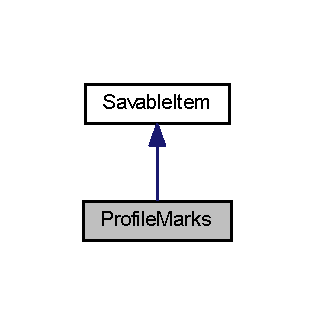
\includegraphics[width=151pt]{class_profile_marks__inherit__graph}
\end{center}
\end{figure}


Граф связей класса Profile\-Marks\-:
\nopagebreak
\begin{figure}[H]
\begin{center}
\leavevmode
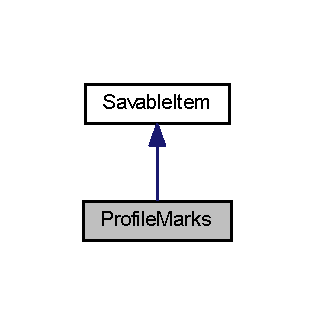
\includegraphics[width=151pt]{class_profile_marks__coll__graph}
\end{center}
\end{figure}
\subsection*{Открытые члены}
\begin{DoxyCompactItemize}
\item 
\hyperlink{class_profile_marks_ac1d9331398f1091f03000fb70b4cebd0}{Profile\-Marks} (void)
\item 
\hyperlink{class_profile_marks_a74ad8199d7206269b733404f4b693573}{$\sim$\-Profile\-Marks} (void)
\item 
void \hyperlink{class_profile_marks_aa7966667f1baa875bc2bd8db7d909a37}{On\-Draw} (H\-D\-C hdc, const P\-O\-I\-N\-T $\ast$p\-Points, unsigned n\-Count)
\item 
void \hyperlink{class_profile_marks_ab243c85d1dc29170f18ae4c4a20ed789}{Pre\-Draw} (H\-D\-C hdc)
\item 
int \hyperlink{class_profile_marks_a051a19747efe246de75f7fc85ffd70ef}{Get\-Frequency} () const 
\item 
void \hyperlink{class_profile_marks_a1413fe406c87a46c8967c90b2dcd8dbe}{Set\-Frequency} (const int n\-Freq)
\item 
int \hyperlink{class_profile_marks_aa0d8285f49f82349a05303ce91e8aed5}{Get\-Size} () const 
\item 
void \hyperlink{class_profile_marks_a53183bc811f6dba3002f5c1f1ced8d18}{Set\-Size} (const int n\-Size)
\item 
C\-O\-L\-O\-R\-R\-E\-F \hyperlink{class_profile_marks_a412ce6c7398fe1e937d077c651bc6be9}{Get\-Line\-Color} () const 
\item 
void \hyperlink{class_profile_marks_a77b56c9b9d21376533dae53cee0a6f26}{Set\-Line\-Color} (const C\-O\-L\-O\-R\-R\-E\-F clr\-Line)
\item 
C\-O\-L\-O\-R\-R\-E\-F \hyperlink{class_profile_marks_a191e51521d74dd8210ae02260c1bf1b1}{Get\-Fill\-Color} () const 
\item 
void \hyperlink{class_profile_marks_aa6bcbcdbadf04e61e4b6c071f7541225}{Set\-Fill\-Color} (const C\-O\-L\-O\-R\-R\-E\-F clr\-Fill)
\item 
void \hyperlink{class_profile_marks_a178920b4ff1861824fcdc617ed872f55}{Set\-Mark\-Type} (const int n\-Type)
\item 
int \hyperlink{class_profile_marks_a6823d42202f99941e5c92008b9dbf4d1}{Get\-Mark\-Type} () const 
\item 
void \hyperlink{class_profile_marks_af6f6413f5d507f714cc9c38f228da4ce}{Enable} (B\-O\-O\-L enable=T\-R\-U\-E)
\item 
B\-O\-O\-L \hyperlink{class_profile_marks_a5edbf30ca2bff84f8736aad24d231795}{Is\-Enabled} () const 
\item 
virtual B\-O\-O\-L \hyperlink{class_profile_marks_a6f0d5141d95c02bc92ebb5ce9e96d559}{Write} (H\-A\-N\-D\-L\-E h\-File) const 
\item 
virtual B\-O\-O\-L \hyperlink{class_profile_marks_af10107761b4341881739dc5d2f574b53}{Read} (H\-A\-N\-D\-L\-E h\-File)
\end{DoxyCompactItemize}
\subsection*{Дополнительные унаследованные члены}


\subsection{Конструктор(ы)}
\hypertarget{class_profile_marks_ac1d9331398f1091f03000fb70b4cebd0}{\index{Profile\-Marks@{Profile\-Marks}!Profile\-Marks@{Profile\-Marks}}
\index{Profile\-Marks@{Profile\-Marks}!ProfileMarks@{Profile\-Marks}}
\subsubsection[{Profile\-Marks}]{\setlength{\rightskip}{0pt plus 5cm}Profile\-Marks\-::\-Profile\-Marks (
\begin{DoxyParamCaption}
\item[{void}]{}
\end{DoxyParamCaption}
)}}\label{class_profile_marks_ac1d9331398f1091f03000fb70b4cebd0}
\hypertarget{class_profile_marks_a74ad8199d7206269b733404f4b693573}{\index{Profile\-Marks@{Profile\-Marks}!$\sim$\-Profile\-Marks@{$\sim$\-Profile\-Marks}}
\index{$\sim$\-Profile\-Marks@{$\sim$\-Profile\-Marks}!ProfileMarks@{Profile\-Marks}}
\subsubsection[{$\sim$\-Profile\-Marks}]{\setlength{\rightskip}{0pt plus 5cm}Profile\-Marks\-::$\sim$\-Profile\-Marks (
\begin{DoxyParamCaption}
\item[{void}]{}
\end{DoxyParamCaption}
)}}\label{class_profile_marks_a74ad8199d7206269b733404f4b693573}


\subsection{Методы}
\hypertarget{class_profile_marks_af6f6413f5d507f714cc9c38f228da4ce}{\index{Profile\-Marks@{Profile\-Marks}!Enable@{Enable}}
\index{Enable@{Enable}!ProfileMarks@{Profile\-Marks}}
\subsubsection[{Enable}]{\setlength{\rightskip}{0pt plus 5cm}void Profile\-Marks\-::\-Enable (
\begin{DoxyParamCaption}
\item[{B\-O\-O\-L}]{enable = {\ttfamily TRUE}}
\end{DoxyParamCaption}
)\hspace{0.3cm}{\ttfamily [inline]}}}\label{class_profile_marks_af6f6413f5d507f714cc9c38f228da4ce}
\hypertarget{class_profile_marks_a191e51521d74dd8210ae02260c1bf1b1}{\index{Profile\-Marks@{Profile\-Marks}!Get\-Fill\-Color@{Get\-Fill\-Color}}
\index{Get\-Fill\-Color@{Get\-Fill\-Color}!ProfileMarks@{Profile\-Marks}}
\subsubsection[{Get\-Fill\-Color}]{\setlength{\rightskip}{0pt plus 5cm}C\-O\-L\-O\-R\-R\-E\-F Profile\-Marks\-::\-Get\-Fill\-Color (
\begin{DoxyParamCaption}
{}
\end{DoxyParamCaption}
) const\hspace{0.3cm}{\ttfamily [inline]}}}\label{class_profile_marks_a191e51521d74dd8210ae02260c1bf1b1}
\hypertarget{class_profile_marks_a051a19747efe246de75f7fc85ffd70ef}{\index{Profile\-Marks@{Profile\-Marks}!Get\-Frequency@{Get\-Frequency}}
\index{Get\-Frequency@{Get\-Frequency}!ProfileMarks@{Profile\-Marks}}
\subsubsection[{Get\-Frequency}]{\setlength{\rightskip}{0pt plus 5cm}int Profile\-Marks\-::\-Get\-Frequency (
\begin{DoxyParamCaption}
{}
\end{DoxyParamCaption}
) const\hspace{0.3cm}{\ttfamily [inline]}}}\label{class_profile_marks_a051a19747efe246de75f7fc85ffd70ef}
\hypertarget{class_profile_marks_a412ce6c7398fe1e937d077c651bc6be9}{\index{Profile\-Marks@{Profile\-Marks}!Get\-Line\-Color@{Get\-Line\-Color}}
\index{Get\-Line\-Color@{Get\-Line\-Color}!ProfileMarks@{Profile\-Marks}}
\subsubsection[{Get\-Line\-Color}]{\setlength{\rightskip}{0pt plus 5cm}C\-O\-L\-O\-R\-R\-E\-F Profile\-Marks\-::\-Get\-Line\-Color (
\begin{DoxyParamCaption}
{}
\end{DoxyParamCaption}
) const\hspace{0.3cm}{\ttfamily [inline]}}}\label{class_profile_marks_a412ce6c7398fe1e937d077c651bc6be9}
\hypertarget{class_profile_marks_a6823d42202f99941e5c92008b9dbf4d1}{\index{Profile\-Marks@{Profile\-Marks}!Get\-Mark\-Type@{Get\-Mark\-Type}}
\index{Get\-Mark\-Type@{Get\-Mark\-Type}!ProfileMarks@{Profile\-Marks}}
\subsubsection[{Get\-Mark\-Type}]{\setlength{\rightskip}{0pt plus 5cm}int Profile\-Marks\-::\-Get\-Mark\-Type (
\begin{DoxyParamCaption}
{}
\end{DoxyParamCaption}
) const\hspace{0.3cm}{\ttfamily [inline]}}}\label{class_profile_marks_a6823d42202f99941e5c92008b9dbf4d1}
\hypertarget{class_profile_marks_aa0d8285f49f82349a05303ce91e8aed5}{\index{Profile\-Marks@{Profile\-Marks}!Get\-Size@{Get\-Size}}
\index{Get\-Size@{Get\-Size}!ProfileMarks@{Profile\-Marks}}
\subsubsection[{Get\-Size}]{\setlength{\rightskip}{0pt plus 5cm}int Profile\-Marks\-::\-Get\-Size (
\begin{DoxyParamCaption}
{}
\end{DoxyParamCaption}
) const\hspace{0.3cm}{\ttfamily [inline]}}}\label{class_profile_marks_aa0d8285f49f82349a05303ce91e8aed5}
\hypertarget{class_profile_marks_a5edbf30ca2bff84f8736aad24d231795}{\index{Profile\-Marks@{Profile\-Marks}!Is\-Enabled@{Is\-Enabled}}
\index{Is\-Enabled@{Is\-Enabled}!ProfileMarks@{Profile\-Marks}}
\subsubsection[{Is\-Enabled}]{\setlength{\rightskip}{0pt plus 5cm}B\-O\-O\-L Profile\-Marks\-::\-Is\-Enabled (
\begin{DoxyParamCaption}
{}
\end{DoxyParamCaption}
) const\hspace{0.3cm}{\ttfamily [inline]}}}\label{class_profile_marks_a5edbf30ca2bff84f8736aad24d231795}
\hypertarget{class_profile_marks_aa7966667f1baa875bc2bd8db7d909a37}{\index{Profile\-Marks@{Profile\-Marks}!On\-Draw@{On\-Draw}}
\index{On\-Draw@{On\-Draw}!ProfileMarks@{Profile\-Marks}}
\subsubsection[{On\-Draw}]{\setlength{\rightskip}{0pt plus 5cm}void Profile\-Marks\-::\-On\-Draw (
\begin{DoxyParamCaption}
\item[{H\-D\-C}]{hdc, }
\item[{const P\-O\-I\-N\-T $\ast$}]{p\-Points, }
\item[{unsigned}]{n\-Count}
\end{DoxyParamCaption}
)}}\label{class_profile_marks_aa7966667f1baa875bc2bd8db7d909a37}
\hypertarget{class_profile_marks_ab243c85d1dc29170f18ae4c4a20ed789}{\index{Profile\-Marks@{Profile\-Marks}!Pre\-Draw@{Pre\-Draw}}
\index{Pre\-Draw@{Pre\-Draw}!ProfileMarks@{Profile\-Marks}}
\subsubsection[{Pre\-Draw}]{\setlength{\rightskip}{0pt plus 5cm}void Profile\-Marks\-::\-Pre\-Draw (
\begin{DoxyParamCaption}
\item[{H\-D\-C}]{hdc}
\end{DoxyParamCaption}
)}}\label{class_profile_marks_ab243c85d1dc29170f18ae4c4a20ed789}
\hypertarget{class_profile_marks_af10107761b4341881739dc5d2f574b53}{\index{Profile\-Marks@{Profile\-Marks}!Read@{Read}}
\index{Read@{Read}!ProfileMarks@{Profile\-Marks}}
\subsubsection[{Read}]{\setlength{\rightskip}{0pt plus 5cm}B\-O\-O\-L Profile\-Marks\-::\-Read (
\begin{DoxyParamCaption}
\item[{H\-A\-N\-D\-L\-E}]{h\-File}
\end{DoxyParamCaption}
)\hspace{0.3cm}{\ttfamily [virtual]}}}\label{class_profile_marks_af10107761b4341881739dc5d2f574b53}


Замещает \hyperlink{class_savable_item_a7eadd16b2cb0652091cc15f596a00fb2}{Savable\-Item}.

\hypertarget{class_profile_marks_aa6bcbcdbadf04e61e4b6c071f7541225}{\index{Profile\-Marks@{Profile\-Marks}!Set\-Fill\-Color@{Set\-Fill\-Color}}
\index{Set\-Fill\-Color@{Set\-Fill\-Color}!ProfileMarks@{Profile\-Marks}}
\subsubsection[{Set\-Fill\-Color}]{\setlength{\rightskip}{0pt plus 5cm}void Profile\-Marks\-::\-Set\-Fill\-Color (
\begin{DoxyParamCaption}
\item[{const C\-O\-L\-O\-R\-R\-E\-F}]{clr\-Fill}
\end{DoxyParamCaption}
)\hspace{0.3cm}{\ttfamily [inline]}}}\label{class_profile_marks_aa6bcbcdbadf04e61e4b6c071f7541225}
\hypertarget{class_profile_marks_a1413fe406c87a46c8967c90b2dcd8dbe}{\index{Profile\-Marks@{Profile\-Marks}!Set\-Frequency@{Set\-Frequency}}
\index{Set\-Frequency@{Set\-Frequency}!ProfileMarks@{Profile\-Marks}}
\subsubsection[{Set\-Frequency}]{\setlength{\rightskip}{0pt plus 5cm}void Profile\-Marks\-::\-Set\-Frequency (
\begin{DoxyParamCaption}
\item[{const int}]{n\-Freq}
\end{DoxyParamCaption}
)\hspace{0.3cm}{\ttfamily [inline]}}}\label{class_profile_marks_a1413fe406c87a46c8967c90b2dcd8dbe}
\hypertarget{class_profile_marks_a77b56c9b9d21376533dae53cee0a6f26}{\index{Profile\-Marks@{Profile\-Marks}!Set\-Line\-Color@{Set\-Line\-Color}}
\index{Set\-Line\-Color@{Set\-Line\-Color}!ProfileMarks@{Profile\-Marks}}
\subsubsection[{Set\-Line\-Color}]{\setlength{\rightskip}{0pt plus 5cm}void Profile\-Marks\-::\-Set\-Line\-Color (
\begin{DoxyParamCaption}
\item[{const C\-O\-L\-O\-R\-R\-E\-F}]{clr\-Line}
\end{DoxyParamCaption}
)\hspace{0.3cm}{\ttfamily [inline]}}}\label{class_profile_marks_a77b56c9b9d21376533dae53cee0a6f26}
\hypertarget{class_profile_marks_a178920b4ff1861824fcdc617ed872f55}{\index{Profile\-Marks@{Profile\-Marks}!Set\-Mark\-Type@{Set\-Mark\-Type}}
\index{Set\-Mark\-Type@{Set\-Mark\-Type}!ProfileMarks@{Profile\-Marks}}
\subsubsection[{Set\-Mark\-Type}]{\setlength{\rightskip}{0pt plus 5cm}void Profile\-Marks\-::\-Set\-Mark\-Type (
\begin{DoxyParamCaption}
\item[{const int}]{n\-Type}
\end{DoxyParamCaption}
)\hspace{0.3cm}{\ttfamily [inline]}}}\label{class_profile_marks_a178920b4ff1861824fcdc617ed872f55}
\hypertarget{class_profile_marks_a53183bc811f6dba3002f5c1f1ced8d18}{\index{Profile\-Marks@{Profile\-Marks}!Set\-Size@{Set\-Size}}
\index{Set\-Size@{Set\-Size}!ProfileMarks@{Profile\-Marks}}
\subsubsection[{Set\-Size}]{\setlength{\rightskip}{0pt plus 5cm}void Profile\-Marks\-::\-Set\-Size (
\begin{DoxyParamCaption}
\item[{const int}]{n\-Size}
\end{DoxyParamCaption}
)\hspace{0.3cm}{\ttfamily [inline]}}}\label{class_profile_marks_a53183bc811f6dba3002f5c1f1ced8d18}
\hypertarget{class_profile_marks_a6f0d5141d95c02bc92ebb5ce9e96d559}{\index{Profile\-Marks@{Profile\-Marks}!Write@{Write}}
\index{Write@{Write}!ProfileMarks@{Profile\-Marks}}
\subsubsection[{Write}]{\setlength{\rightskip}{0pt plus 5cm}B\-O\-O\-L Profile\-Marks\-::\-Write (
\begin{DoxyParamCaption}
\item[{H\-A\-N\-D\-L\-E}]{h\-File}
\end{DoxyParamCaption}
) const\hspace{0.3cm}{\ttfamily [virtual]}}}\label{class_profile_marks_a6f0d5141d95c02bc92ebb5ce9e96d559}


Замещает \hyperlink{class_savable_item_a0da511a4854f515096f8f9b498f64158}{Savable\-Item}.



Объявления и описания членов классов находятся в файлах\-:\begin{DoxyCompactItemize}
\item 
src/\hyperlink{_profile_marks_8h}{Profile\-Marks.\-h}\item 
src/\hyperlink{_profile_marks_8cpp}{Profile\-Marks.\-cpp}\end{DoxyCompactItemize}

\hypertarget{class_r_t_f_string}{\section{Класс R\-T\-F\-String}
\label{class_r_t_f_string}\index{R\-T\-F\-String@{R\-T\-F\-String}}
}


{\ttfamily \#include $<$rtfstring.\-h$>$}



Граф связей класса R\-T\-F\-String\-:
\nopagebreak
\begin{figure}[H]
\begin{center}
\leavevmode
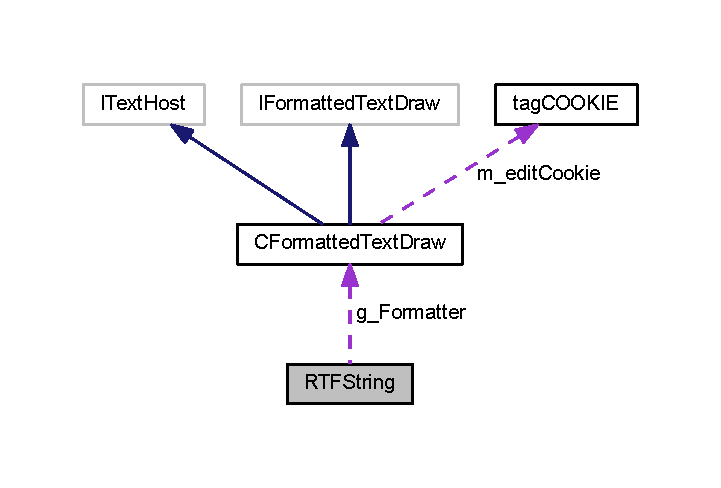
\includegraphics[width=346pt]{class_r_t_f_string__coll__graph}
\end{center}
\end{figure}
\subsection*{Открытые члены}
\begin{DoxyCompactItemize}
\item 
\hyperlink{class_r_t_f_string_a51863fc1577a626c5a4ccb15e6764073}{R\-T\-F\-String} (H\-M\-O\-D\-U\-L\-E hmod)
\item 
\hyperlink{class_r_t_f_string_a018b3244fc6039305ce5407936a9992e}{R\-T\-F\-String} (const \hyperlink{class_r_t_f_string}{R\-T\-F\-String} \&rhs)
\item 
\hyperlink{class_r_t_f_string_a63309fd7a3d4189fa2b6d2525d718d42}{$\sim$\-R\-T\-F\-String} ()
\item 
const \hyperlink{class_r_t_f_string}{R\-T\-F\-String} \& \hyperlink{class_r_t_f_string_a2e4c798c305f06b68fdbd5a5d91f0c8a}{operator=} (const \hyperlink{class_r_t_f_string}{R\-T\-F\-String} \&rhs)
\item 
void \hyperlink{class_r_t_f_string_aa011f163ea938fd7c24dc55001afa34b}{Set\-Text} (std\-::string title)
\item 
const std\-::string \& \hyperlink{class_r_t_f_string_a0847a69aa9573d5b298c2b181f98450c}{Get\-Text} () const 
\item 
void \hyperlink{class_r_t_f_string_af5be9c1a74068a8d1f805e093451be51}{Set\-Color} (C\-O\-L\-O\-R\-R\-E\-F clr)
\item 
void \hyperlink{class_r_t_f_string_ae7130e8d2df43ae9b821fe70804f1e4c}{Set\-Font} (const L\-O\-G\-F\-O\-N\-T $\ast$const plf)
\item 
B\-O\-O\-L \hyperlink{class_r_t_f_string_a63a4f84996a98bd0f1901eff5017fbb2}{Write} (H\-A\-N\-D\-L\-E h\-File) const 
\item 
B\-O\-O\-L \hyperlink{class_r_t_f_string_aa91f1cca43e34327c3ffabdd6c928871}{Read} (H\-A\-N\-D\-L\-E h\-File)
\item 
void \hyperlink{class_r_t_f_string_a1095cfa000481881825a6973506cdcc9}{Get\-Dimensions} (S\-I\-Z\-E \&size) const 
\item 
void \hyperlink{class_r_t_f_string_a8d9b2138da58d424b9bc8df251468b2e}{Set\-Orientation} (int degrees)
\item 
int \hyperlink{class_r_t_f_string_a04121663e4ab24711fe949750dc2b5ee}{Get\-Orientation} () const 
\item 
void \hyperlink{class_r_t_f_string_a45a11ee69611ed59989989b2d39133b8}{Draw} (H\-D\-C hdc, int x, int y) const 
\end{DoxyCompactItemize}
\subsection*{Открытые статические члены}
\begin{DoxyCompactItemize}
\item 
static std\-::string \hyperlink{class_r_t_f_string_a94673f221d744299393675f9b0e115b5}{Read\-String} (H\-A\-N\-D\-L\-E h\-File)
\item 
static B\-O\-O\-L \hyperlink{class_r_t_f_string_a15525dd2260dc2c4ba825a8b6db3db7a}{Write\-String} (H\-A\-N\-D\-L\-E h\-File, std\-::string the\-String)
\end{DoxyCompactItemize}
\subsection*{Защищенные данные}
\begin{DoxyCompactItemize}
\item 
std\-::string \hyperlink{class_r_t_f_string_ade9f23f1498c4102691b4dcf03af5435}{str\-Title}
\item 
int \hyperlink{class_r_t_f_string_a56d829be2f4b7cf88f661d52c9d794ef}{orientation}
\item 
\hyperlink{class_c_formatted_text_draw}{C\-Formatted\-Text\-Draw} $\ast$ \hyperlink{class_r_t_f_string_af121473f7d2ca2939cae4dde99ad3506}{g\-\_\-\-Formatter}
\end{DoxyCompactItemize}


\subsection{Конструктор(ы)}
\hypertarget{class_r_t_f_string_a51863fc1577a626c5a4ccb15e6764073}{\index{R\-T\-F\-String@{R\-T\-F\-String}!R\-T\-F\-String@{R\-T\-F\-String}}
\index{R\-T\-F\-String@{R\-T\-F\-String}!RTFString@{R\-T\-F\-String}}
\subsubsection[{R\-T\-F\-String}]{\setlength{\rightskip}{0pt plus 5cm}R\-T\-F\-String\-::\-R\-T\-F\-String (
\begin{DoxyParamCaption}
\item[{H\-M\-O\-D\-U\-L\-E}]{hmod}
\end{DoxyParamCaption}
)}}\label{class_r_t_f_string_a51863fc1577a626c5a4ccb15e6764073}
\hypertarget{class_r_t_f_string_a018b3244fc6039305ce5407936a9992e}{\index{R\-T\-F\-String@{R\-T\-F\-String}!R\-T\-F\-String@{R\-T\-F\-String}}
\index{R\-T\-F\-String@{R\-T\-F\-String}!RTFString@{R\-T\-F\-String}}
\subsubsection[{R\-T\-F\-String}]{\setlength{\rightskip}{0pt plus 5cm}R\-T\-F\-String\-::\-R\-T\-F\-String (
\begin{DoxyParamCaption}
\item[{const {\bf R\-T\-F\-String} \&}]{rhs}
\end{DoxyParamCaption}
)\hspace{0.3cm}{\ttfamily [inline]}}}\label{class_r_t_f_string_a018b3244fc6039305ce5407936a9992e}
\hypertarget{class_r_t_f_string_a63309fd7a3d4189fa2b6d2525d718d42}{\index{R\-T\-F\-String@{R\-T\-F\-String}!$\sim$\-R\-T\-F\-String@{$\sim$\-R\-T\-F\-String}}
\index{$\sim$\-R\-T\-F\-String@{$\sim$\-R\-T\-F\-String}!RTFString@{R\-T\-F\-String}}
\subsubsection[{$\sim$\-R\-T\-F\-String}]{\setlength{\rightskip}{0pt plus 5cm}R\-T\-F\-String\-::$\sim$\-R\-T\-F\-String (
\begin{DoxyParamCaption}
{}
\end{DoxyParamCaption}
)}}\label{class_r_t_f_string_a63309fd7a3d4189fa2b6d2525d718d42}


\subsection{Методы}
\hypertarget{class_r_t_f_string_a45a11ee69611ed59989989b2d39133b8}{\index{R\-T\-F\-String@{R\-T\-F\-String}!Draw@{Draw}}
\index{Draw@{Draw}!RTFString@{R\-T\-F\-String}}
\subsubsection[{Draw}]{\setlength{\rightskip}{0pt plus 5cm}void R\-T\-F\-String\-::\-Draw (
\begin{DoxyParamCaption}
\item[{H\-D\-C}]{hdc, }
\item[{int}]{x, }
\item[{int}]{y}
\end{DoxyParamCaption}
) const}}\label{class_r_t_f_string_a45a11ee69611ed59989989b2d39133b8}
\hypertarget{class_r_t_f_string_a1095cfa000481881825a6973506cdcc9}{\index{R\-T\-F\-String@{R\-T\-F\-String}!Get\-Dimensions@{Get\-Dimensions}}
\index{Get\-Dimensions@{Get\-Dimensions}!RTFString@{R\-T\-F\-String}}
\subsubsection[{Get\-Dimensions}]{\setlength{\rightskip}{0pt plus 5cm}void R\-T\-F\-String\-::\-Get\-Dimensions (
\begin{DoxyParamCaption}
\item[{S\-I\-Z\-E \&}]{size}
\end{DoxyParamCaption}
) const}}\label{class_r_t_f_string_a1095cfa000481881825a6973506cdcc9}
\hypertarget{class_r_t_f_string_a04121663e4ab24711fe949750dc2b5ee}{\index{R\-T\-F\-String@{R\-T\-F\-String}!Get\-Orientation@{Get\-Orientation}}
\index{Get\-Orientation@{Get\-Orientation}!RTFString@{R\-T\-F\-String}}
\subsubsection[{Get\-Orientation}]{\setlength{\rightskip}{0pt plus 5cm}int R\-T\-F\-String\-::\-Get\-Orientation (
\begin{DoxyParamCaption}
{}
\end{DoxyParamCaption}
) const\hspace{0.3cm}{\ttfamily [inline]}}}\label{class_r_t_f_string_a04121663e4ab24711fe949750dc2b5ee}
\hypertarget{class_r_t_f_string_a0847a69aa9573d5b298c2b181f98450c}{\index{R\-T\-F\-String@{R\-T\-F\-String}!Get\-Text@{Get\-Text}}
\index{Get\-Text@{Get\-Text}!RTFString@{R\-T\-F\-String}}
\subsubsection[{Get\-Text}]{\setlength{\rightskip}{0pt plus 5cm}const std\-::string \& R\-T\-F\-String\-::\-Get\-Text (
\begin{DoxyParamCaption}
{}
\end{DoxyParamCaption}
) const}}\label{class_r_t_f_string_a0847a69aa9573d5b298c2b181f98450c}
\hypertarget{class_r_t_f_string_a2e4c798c305f06b68fdbd5a5d91f0c8a}{\index{R\-T\-F\-String@{R\-T\-F\-String}!operator=@{operator=}}
\index{operator=@{operator=}!RTFString@{R\-T\-F\-String}}
\subsubsection[{operator=}]{\setlength{\rightskip}{0pt plus 5cm}const {\bf R\-T\-F\-String} \& R\-T\-F\-String\-::operator= (
\begin{DoxyParamCaption}
\item[{const {\bf R\-T\-F\-String} \&}]{rhs}
\end{DoxyParamCaption}
)}}\label{class_r_t_f_string_a2e4c798c305f06b68fdbd5a5d91f0c8a}
\hypertarget{class_r_t_f_string_aa91f1cca43e34327c3ffabdd6c928871}{\index{R\-T\-F\-String@{R\-T\-F\-String}!Read@{Read}}
\index{Read@{Read}!RTFString@{R\-T\-F\-String}}
\subsubsection[{Read}]{\setlength{\rightskip}{0pt plus 5cm}B\-O\-O\-L R\-T\-F\-String\-::\-Read (
\begin{DoxyParamCaption}
\item[{H\-A\-N\-D\-L\-E}]{h\-File}
\end{DoxyParamCaption}
)}}\label{class_r_t_f_string_aa91f1cca43e34327c3ffabdd6c928871}
\hypertarget{class_r_t_f_string_a94673f221d744299393675f9b0e115b5}{\index{R\-T\-F\-String@{R\-T\-F\-String}!Read\-String@{Read\-String}}
\index{Read\-String@{Read\-String}!RTFString@{R\-T\-F\-String}}
\subsubsection[{Read\-String}]{\setlength{\rightskip}{0pt plus 5cm}std\-::string R\-T\-F\-String\-::\-Read\-String (
\begin{DoxyParamCaption}
\item[{H\-A\-N\-D\-L\-E}]{h\-File}
\end{DoxyParamCaption}
)\hspace{0.3cm}{\ttfamily [static]}}}\label{class_r_t_f_string_a94673f221d744299393675f9b0e115b5}
\hypertarget{class_r_t_f_string_af5be9c1a74068a8d1f805e093451be51}{\index{R\-T\-F\-String@{R\-T\-F\-String}!Set\-Color@{Set\-Color}}
\index{Set\-Color@{Set\-Color}!RTFString@{R\-T\-F\-String}}
\subsubsection[{Set\-Color}]{\setlength{\rightskip}{0pt plus 5cm}void R\-T\-F\-String\-::\-Set\-Color (
\begin{DoxyParamCaption}
\item[{C\-O\-L\-O\-R\-R\-E\-F}]{clr}
\end{DoxyParamCaption}
)}}\label{class_r_t_f_string_af5be9c1a74068a8d1f805e093451be51}
\hypertarget{class_r_t_f_string_ae7130e8d2df43ae9b821fe70804f1e4c}{\index{R\-T\-F\-String@{R\-T\-F\-String}!Set\-Font@{Set\-Font}}
\index{Set\-Font@{Set\-Font}!RTFString@{R\-T\-F\-String}}
\subsubsection[{Set\-Font}]{\setlength{\rightskip}{0pt plus 5cm}void R\-T\-F\-String\-::\-Set\-Font (
\begin{DoxyParamCaption}
\item[{const L\-O\-G\-F\-O\-N\-T $\ast$const}]{plf}
\end{DoxyParamCaption}
)}}\label{class_r_t_f_string_ae7130e8d2df43ae9b821fe70804f1e4c}
\hypertarget{class_r_t_f_string_a8d9b2138da58d424b9bc8df251468b2e}{\index{R\-T\-F\-String@{R\-T\-F\-String}!Set\-Orientation@{Set\-Orientation}}
\index{Set\-Orientation@{Set\-Orientation}!RTFString@{R\-T\-F\-String}}
\subsubsection[{Set\-Orientation}]{\setlength{\rightskip}{0pt plus 5cm}void R\-T\-F\-String\-::\-Set\-Orientation (
\begin{DoxyParamCaption}
\item[{int}]{degrees}
\end{DoxyParamCaption}
)\hspace{0.3cm}{\ttfamily [inline]}}}\label{class_r_t_f_string_a8d9b2138da58d424b9bc8df251468b2e}
\hypertarget{class_r_t_f_string_aa011f163ea938fd7c24dc55001afa34b}{\index{R\-T\-F\-String@{R\-T\-F\-String}!Set\-Text@{Set\-Text}}
\index{Set\-Text@{Set\-Text}!RTFString@{R\-T\-F\-String}}
\subsubsection[{Set\-Text}]{\setlength{\rightskip}{0pt plus 5cm}void R\-T\-F\-String\-::\-Set\-Text (
\begin{DoxyParamCaption}
\item[{std\-::string}]{title}
\end{DoxyParamCaption}
)}}\label{class_r_t_f_string_aa011f163ea938fd7c24dc55001afa34b}
\hypertarget{class_r_t_f_string_a63a4f84996a98bd0f1901eff5017fbb2}{\index{R\-T\-F\-String@{R\-T\-F\-String}!Write@{Write}}
\index{Write@{Write}!RTFString@{R\-T\-F\-String}}
\subsubsection[{Write}]{\setlength{\rightskip}{0pt plus 5cm}B\-O\-O\-L R\-T\-F\-String\-::\-Write (
\begin{DoxyParamCaption}
\item[{H\-A\-N\-D\-L\-E}]{h\-File}
\end{DoxyParamCaption}
) const}}\label{class_r_t_f_string_a63a4f84996a98bd0f1901eff5017fbb2}
\hypertarget{class_r_t_f_string_a15525dd2260dc2c4ba825a8b6db3db7a}{\index{R\-T\-F\-String@{R\-T\-F\-String}!Write\-String@{Write\-String}}
\index{Write\-String@{Write\-String}!RTFString@{R\-T\-F\-String}}
\subsubsection[{Write\-String}]{\setlength{\rightskip}{0pt plus 5cm}B\-O\-O\-L R\-T\-F\-String\-::\-Write\-String (
\begin{DoxyParamCaption}
\item[{H\-A\-N\-D\-L\-E}]{h\-File, }
\item[{std\-::string}]{the\-String}
\end{DoxyParamCaption}
)\hspace{0.3cm}{\ttfamily [static]}}}\label{class_r_t_f_string_a15525dd2260dc2c4ba825a8b6db3db7a}


\subsection{Данные класса}
\hypertarget{class_r_t_f_string_af121473f7d2ca2939cae4dde99ad3506}{\index{R\-T\-F\-String@{R\-T\-F\-String}!g\-\_\-\-Formatter@{g\-\_\-\-Formatter}}
\index{g\-\_\-\-Formatter@{g\-\_\-\-Formatter}!RTFString@{R\-T\-F\-String}}
\subsubsection[{g\-\_\-\-Formatter}]{\setlength{\rightskip}{0pt plus 5cm}{\bf C\-Formatted\-Text\-Draw}$\ast$ R\-T\-F\-String\-::g\-\_\-\-Formatter\hspace{0.3cm}{\ttfamily [protected]}}}\label{class_r_t_f_string_af121473f7d2ca2939cae4dde99ad3506}
\hypertarget{class_r_t_f_string_a56d829be2f4b7cf88f661d52c9d794ef}{\index{R\-T\-F\-String@{R\-T\-F\-String}!orientation@{orientation}}
\index{orientation@{orientation}!RTFString@{R\-T\-F\-String}}
\subsubsection[{orientation}]{\setlength{\rightskip}{0pt plus 5cm}int R\-T\-F\-String\-::orientation\hspace{0.3cm}{\ttfamily [protected]}}}\label{class_r_t_f_string_a56d829be2f4b7cf88f661d52c9d794ef}
\hypertarget{class_r_t_f_string_ade9f23f1498c4102691b4dcf03af5435}{\index{R\-T\-F\-String@{R\-T\-F\-String}!str\-Title@{str\-Title}}
\index{str\-Title@{str\-Title}!RTFString@{R\-T\-F\-String}}
\subsubsection[{str\-Title}]{\setlength{\rightskip}{0pt plus 5cm}std\-::string R\-T\-F\-String\-::str\-Title\hspace{0.3cm}{\ttfamily [protected]}}}\label{class_r_t_f_string_ade9f23f1498c4102691b4dcf03af5435}


Объявления и описания членов классов находятся в файлах\-:\begin{DoxyCompactItemize}
\item 
src/\hyperlink{rtfstring_8h}{rtfstring.\-h}\item 
src/\hyperlink{rtfstring_8cpp}{rtfstring.\-cpp}\end{DoxyCompactItemize}

\hypertarget{class_savable_item}{\section{Класс Savable\-Item}
\label{class_savable_item}\index{Savable\-Item@{Savable\-Item}}
}


{\ttfamily \#include $<$Savable\-Item.\-h$>$}



Граф наследования\-:Savable\-Item\-:
\nopagebreak
\begin{figure}[H]
\begin{center}
\leavevmode
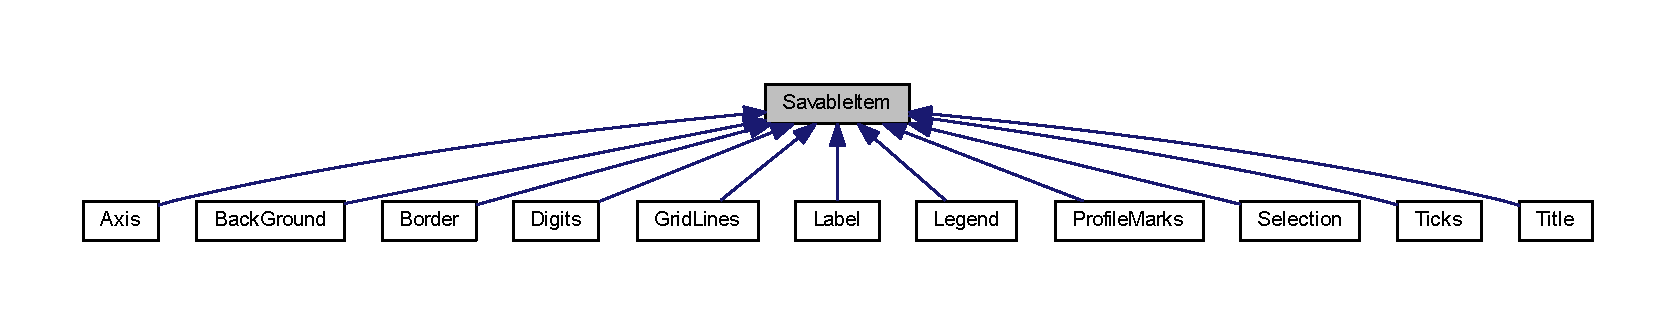
\includegraphics[width=350pt]{class_savable_item__inherit__graph}
\end{center}
\end{figure}
\subsection*{Открытые члены}
\begin{DoxyCompactItemize}
\item 
\hyperlink{class_savable_item_ab046904bea3b84bd453764fe164fcbd5}{Savable\-Item} ()
\item 
virtual \hyperlink{class_savable_item_a01e2cdaa3e35d16f31337d02e794117e}{$\sim$\-Savable\-Item} ()
\item 
virtual B\-O\-O\-L \hyperlink{class_savable_item_a0da511a4854f515096f8f9b498f64158}{Write} (H\-A\-N\-D\-L\-E h\-File) const =0
\item 
virtual B\-O\-O\-L \hyperlink{class_savable_item_a7eadd16b2cb0652091cc15f596a00fb2}{Read} (H\-A\-N\-D\-L\-E h\-File)=0
\end{DoxyCompactItemize}
\subsection*{Защищенные статические члены}
\begin{DoxyCompactItemize}
\item 
static std\-::string \hyperlink{class_savable_item_ab7fdbc1d0002d102e957104c130678d6}{Read\-String} (H\-A\-N\-D\-L\-E h\-File)
\item 
static B\-O\-O\-L \hyperlink{class_savable_item_a491b89267b8402aeb64bfeda5cef0af1}{Write\-String} (H\-A\-N\-D\-L\-E h\-File, std\-::string the\-String)
\end{DoxyCompactItemize}


\subsection{Конструктор(ы)}
\hypertarget{class_savable_item_ab046904bea3b84bd453764fe164fcbd5}{\index{Savable\-Item@{Savable\-Item}!Savable\-Item@{Savable\-Item}}
\index{Savable\-Item@{Savable\-Item}!SavableItem@{Savable\-Item}}
\subsubsection[{Savable\-Item}]{\setlength{\rightskip}{0pt plus 5cm}Savable\-Item\-::\-Savable\-Item (
\begin{DoxyParamCaption}
{}
\end{DoxyParamCaption}
)\hspace{0.3cm}{\ttfamily [inline]}}}\label{class_savable_item_ab046904bea3b84bd453764fe164fcbd5}
\hypertarget{class_savable_item_a01e2cdaa3e35d16f31337d02e794117e}{\index{Savable\-Item@{Savable\-Item}!$\sim$\-Savable\-Item@{$\sim$\-Savable\-Item}}
\index{$\sim$\-Savable\-Item@{$\sim$\-Savable\-Item}!SavableItem@{Savable\-Item}}
\subsubsection[{$\sim$\-Savable\-Item}]{\setlength{\rightskip}{0pt plus 5cm}virtual Savable\-Item\-::$\sim$\-Savable\-Item (
\begin{DoxyParamCaption}
{}
\end{DoxyParamCaption}
)\hspace{0.3cm}{\ttfamily [inline]}, {\ttfamily [virtual]}}}\label{class_savable_item_a01e2cdaa3e35d16f31337d02e794117e}


\subsection{Методы}
\hypertarget{class_savable_item_a7eadd16b2cb0652091cc15f596a00fb2}{\index{Savable\-Item@{Savable\-Item}!Read@{Read}}
\index{Read@{Read}!SavableItem@{Savable\-Item}}
\subsubsection[{Read}]{\setlength{\rightskip}{0pt plus 5cm}virtual B\-O\-O\-L Savable\-Item\-::\-Read (
\begin{DoxyParamCaption}
\item[{H\-A\-N\-D\-L\-E}]{h\-File}
\end{DoxyParamCaption}
)\hspace{0.3cm}{\ttfamily [pure virtual]}}}\label{class_savable_item_a7eadd16b2cb0652091cc15f596a00fb2}


Замещается в \hyperlink{class_ticks_a6059d8bd2489336d9e77fe7c701e1d20}{Ticks}, \hyperlink{class_axis_af403dc4181f1681d321f190bd74268ff}{Axis}, \hyperlink{class_legend_a881509fdd919ed3a30ca822a5edb1114}{Legend}, \hyperlink{class_back_ground_aba05f03ff7484a1afad33c9400baf644}{Back\-Ground}, \hyperlink{class_digits_a8e4038efd3b350b447a1d509eaa5040e}{Digits}, \hyperlink{class_grid_lines_aecc543959e2bfa9c45345257433a3110}{Grid\-Lines}, \hyperlink{class_label_a491dcc38695f69dd135fba56cfdeb3cf}{Label}, \hyperlink{class_profile_marks_af10107761b4341881739dc5d2f574b53}{Profile\-Marks}, \hyperlink{class_title_ad1cfcfb17962c87f63cae0966d07998c}{Title}, \hyperlink{class_selection_a4cf1ce6c3fb26f950075a17c25341110}{Selection} и \hyperlink{class_border_a35655b3874c3230038e171f18e7286f2}{Border}.

\hypertarget{class_savable_item_ab7fdbc1d0002d102e957104c130678d6}{\index{Savable\-Item@{Savable\-Item}!Read\-String@{Read\-String}}
\index{Read\-String@{Read\-String}!SavableItem@{Savable\-Item}}
\subsubsection[{Read\-String}]{\setlength{\rightskip}{0pt plus 5cm}std\-::string Savable\-Item\-::\-Read\-String (
\begin{DoxyParamCaption}
\item[{H\-A\-N\-D\-L\-E}]{h\-File}
\end{DoxyParamCaption}
)\hspace{0.3cm}{\ttfamily [static]}, {\ttfamily [protected]}}}\label{class_savable_item_ab7fdbc1d0002d102e957104c130678d6}
\hypertarget{class_savable_item_a0da511a4854f515096f8f9b498f64158}{\index{Savable\-Item@{Savable\-Item}!Write@{Write}}
\index{Write@{Write}!SavableItem@{Savable\-Item}}
\subsubsection[{Write}]{\setlength{\rightskip}{0pt plus 5cm}virtual B\-O\-O\-L Savable\-Item\-::\-Write (
\begin{DoxyParamCaption}
\item[{H\-A\-N\-D\-L\-E}]{h\-File}
\end{DoxyParamCaption}
) const\hspace{0.3cm}{\ttfamily [pure virtual]}}}\label{class_savable_item_a0da511a4854f515096f8f9b498f64158}


Замещается в \hyperlink{class_ticks_a49b690623984a9ecc3e2090dac5f0f62}{Ticks}, \hyperlink{class_axis_a895ec09817b379201fe2db2cd1e715aa}{Axis}, \hyperlink{class_legend_a93f2a8366a6c5df1b99d4ba2805928b4}{Legend}, \hyperlink{class_back_ground_ab21bb3686aac638ef0da5fb9a72c3925}{Back\-Ground}, \hyperlink{class_digits_ad516fc5b9c052a5b0b82469e645a5d0a}{Digits}, \hyperlink{class_grid_lines_af41e725b2af5e093e5307e2096c2c4c7}{Grid\-Lines}, \hyperlink{class_label_a244a940c2d9301bd6bd2abcb2ef9af05}{Label}, \hyperlink{class_profile_marks_a6f0d5141d95c02bc92ebb5ce9e96d559}{Profile\-Marks}, \hyperlink{class_title_a3c42069773ac1c18a05ea891b39a3332}{Title}, \hyperlink{class_selection_a1212e14a73f62170020d426c1a3ee5e9}{Selection} и \hyperlink{class_border_a61f82208fd693839acd08d0a4e787b10}{Border}.

\hypertarget{class_savable_item_a491b89267b8402aeb64bfeda5cef0af1}{\index{Savable\-Item@{Savable\-Item}!Write\-String@{Write\-String}}
\index{Write\-String@{Write\-String}!SavableItem@{Savable\-Item}}
\subsubsection[{Write\-String}]{\setlength{\rightskip}{0pt plus 5cm}B\-O\-O\-L Savable\-Item\-::\-Write\-String (
\begin{DoxyParamCaption}
\item[{H\-A\-N\-D\-L\-E}]{h\-File, }
\item[{std\-::string}]{the\-String}
\end{DoxyParamCaption}
)\hspace{0.3cm}{\ttfamily [static]}, {\ttfamily [protected]}}}\label{class_savable_item_a491b89267b8402aeb64bfeda5cef0af1}


Объявления и описания членов классов находятся в файлах\-:\begin{DoxyCompactItemize}
\item 
src/\hyperlink{_savable_item_8h}{Savable\-Item.\-h}\item 
src/\hyperlink{_savable_item_8cpp}{Savable\-Item.\-cpp}\end{DoxyCompactItemize}

\hypertarget{class_selection}{\section{Класс Selection}
\label{class_selection}\index{Selection@{Selection}}
}


{\ttfamily \#include $<$selection.\-h$>$}



Граф наследования\-:Selection\-:
\nopagebreak
\begin{figure}[H]
\begin{center}
\leavevmode
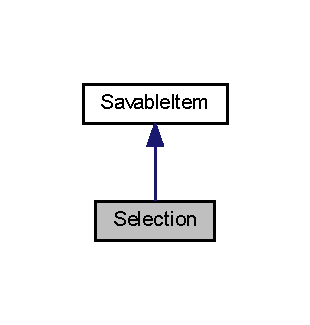
\includegraphics[width=149pt]{class_selection__inherit__graph}
\end{center}
\end{figure}


Граф связей класса Selection\-:
\nopagebreak
\begin{figure}[H]
\begin{center}
\leavevmode
\includegraphics[width=350pt]{class_selection__coll__graph}
\end{center}
\end{figure}
\subsection*{Открытые члены}
\begin{DoxyCompactItemize}
\item 
\hyperlink{class_selection_a1185435bed19519a7b69ef70c679ce70}{Selection} (\hyperlink{class_x_y_plot}{X\-Y\-Plot} $\ast$p\-Plot)
\item 
virtual \hyperlink{class_selection_a1860ec524d11c03de8c10a9354319839}{$\sim$\-Selection} ()
\item 
B\-O\-O\-L \hyperlink{class_selection_afe20319deb65c06229a512f4be84ccd3}{Select} (long I\-D, long index)
\item 
virtual B\-O\-O\-L \hyperlink{class_selection_a1212e14a73f62170020d426c1a3ee5e9}{Write} (H\-A\-N\-D\-L\-E h\-File) const 
\item 
virtual B\-O\-O\-L \hyperlink{class_selection_a4cf1ce6c3fb26f950075a17c25341110}{Read} (H\-A\-N\-D\-L\-E h\-File)
\item 
long \hyperlink{class_selection_a87021f153bfecc0479530578a3f39f00}{Get\-Selection} () const 
\item 
D\-W\-O\-R\-D \hyperlink{class_selection_a0cf4568ea7c9860937d931146e8b99ae}{Get\-Mode} () const 
\item 
D\-W\-O\-R\-D \hyperlink{class_selection_ab0583b6c9cca3ccfee73e3ce587419da}{Set\-Mode} (D\-W\-O\-R\-D dw\-Type)
\item 
void \hyperlink{class_selection_a75530f8982bd489083764cbfff9eefb3}{Set\-Notify\-Message\-I\-D} (long l\-Notify\-Msg)
\item 
void \hyperlink{class_selection_a9e371db3bdd7a9330f83c427a4bcbf0e}{Set\-Flash\-Speed} (\hyperlink{namespacexyplot_aef2fa49b82f49b1152511044149c60bb}{xyplot\-::\-F\-L\-A\-S\-H\-\_\-\-S\-P\-E\-E\-D} fs)
\item 
\hyperlink{namespacexyplot_aef2fa49b82f49b1152511044149c60bb}{xyplot\-::\-F\-L\-A\-S\-H\-\_\-\-S\-P\-E\-E\-D} \hyperlink{class_selection_acc2eec1158e3379e211994a5b3cb0dba}{Get\-Flash\-Speed} () const 
\item 
void \hyperlink{class_selection_abb12cb9336545b1aa4ec1361e08ab5dc}{Resolve\-Plot\-Hit\-Test} (const \hyperlink{selection_8h_adeea1a4ab82509fdc1235948c4efeef6}{L\-P\-P\-L\-O\-T\-H\-I\-T\-T\-E\-S\-T\-R\-E\-S\-U\-L\-T} lpht)
\item 
void \hyperlink{class_selection_a6af1ac7d7f4a22596146c2942d83f15f}{Resolve\-Key\-Press} (long code)
\item 
void \hyperlink{class_selection_ae15010a7dc9450f394a0823cd7a8053f}{On\-Draw} (H\-D\-C hdc, const R\-E\-C\-T rc)
\item 
long \hyperlink{class_selection_a1961c6f204a1bece5bf33e380c8653bf}{Create\-Group} ()
\item 
long \hyperlink{class_selection_a3d3d974a0ecc9336522ddee10271a1f5}{Delete\-Group} (long group)
\item 
long \hyperlink{class_selection_a29137faa8c9270396be41051cef15d69}{Find\-Group} (long profile)
\item 
long \hyperlink{class_selection_a6048c9afc7c6f5f20af089dd1ca9bb29}{Add\-Profile} (long group, long profile)
\end{DoxyCompactItemize}
\subsection*{Защищенные члены}
\begin{DoxyCompactItemize}
\item 
void \hyperlink{class_selection_a240bf3226d6ab1de5e9a958c8940cad7}{Set\-Flash\-State} (B\-O\-O\-L visible)
\item 
void \hyperlink{class_selection_a90033e720a75b54bf8623df01dc16241}{Run\-Flash\-Routine} ()
\item 
void \hyperlink{class_selection_a7a04270c06607b5fae8a182d39bdf301}{Stop\-Flash\-Routine} ()
\end{DoxyCompactItemize}
\subsection*{Защищенные статические члены}
\begin{DoxyCompactItemize}
\item 
static unsigned long \-\_\-\-\_\-stdcall \hyperlink{class_selection_a768b30225e90c1973f3cd895a6ca9709}{fn\-Flash\-Proc} (L\-P\-V\-O\-I\-D lp\-Param)
\end{DoxyCompactItemize}
\subsection*{Защищенные данные}
\begin{DoxyCompactItemize}
\item 
\hyperlink{class_x_y_plot}{X\-Y\-Plot} \& \hyperlink{class_selection_a5446aca339af493b9853e1d8791747ee}{plot}
\item 
\hyperlink{class_profile_group_map}{Profile\-Group\-Map} \hyperlink{class_selection_a9969ae2dd3dfc1de2ff22851f23ca701}{profile\-Group\-Map}
\item 
\hyperlink{profile_8h_ab564cd67657a739c9e5a6caa0ce0dafa}{P\-R\-O\-F\-I\-L\-E\-\_\-\-K\-E\-Y} \hyperlink{class_selection_aad8ed405574d4eaa7c71ea6ab74f921f}{active\-Profile}
\item 
long \hyperlink{class_selection_a3f157e54d3bf571bb58f0ab278311d1f}{active\-Group}
\item 
long \hyperlink{class_selection_ae2e8fd632fbdf5ad8222271d861dee3e}{l\-Notify\-Message}
\item 
unsigned \hyperlink{class_selection_aae0adc2fbecf906fe191f37db02865d9}{selected\-Point\-Ind}
\item 
\hyperlink{class_axis}{Axis} $\ast$ \hyperlink{class_selection_a0e9d894fc2d3922fa13b9bab29c0868b}{active\-Axis}
\item 
\hyperlink{namespacexyplot_aef2fa49b82f49b1152511044149c60bb}{xyplot\-::\-F\-L\-A\-S\-H\-\_\-\-S\-P\-E\-E\-D} \hyperlink{class_selection_ae8158cf33f08749711665081d33a5eee}{m\-\_\-fs}
\item 
\hyperlink{class_line_data}{Line\-Data} \hyperlink{class_selection_a931c1dc1ae09a247eddb870ae860258e}{marker\-Line}
\item 
D\-W\-O\-R\-D \hyperlink{class_selection_abcefb6532a3336dbdb704524ca603f09}{dw\-Selection\-Type}
\item 
P\-O\-I\-N\-T \hyperlink{class_selection_a2ba4d3b1be1be25852a81ae8d8b85464}{pt\-Sel}
\item 
double \hyperlink{class_selection_a55bbd4862d833205e258d2a51256e161}{phys\-Sel\-Point\-X}
\item 
double \hyperlink{class_selection_ae34c8ddfe73abfaaeec3b99bb649f802}{phys\-Sel\-Point\-Y}
\item 
unsigned \hyperlink{class_selection_afe67da14987a0c10aa1f401b4a8210f6}{ellipse\-Radius}
\item 
H\-A\-N\-D\-L\-E \hyperlink{class_selection_aed45afe1b41abebe3f7d22d8b5574ad3}{flash\-Thread}
\item 
H\-A\-N\-D\-L\-E \hyperlink{class_selection_a996d255f46e4aa8d039d17db81026e4e}{ev\-Run\-Flash}
\item 
H\-A\-N\-D\-L\-E \hyperlink{class_selection_a6453d01aeabe2bd18582b71566e84dcc}{ev\-Quit\-Flash}
\item 
C\-R\-I\-T\-I\-C\-A\-L\-\_\-\-S\-E\-C\-T\-I\-O\-N \hyperlink{class_selection_a54afa22854b7ac434dd571dc3d7c4274}{cs}
\item 
unsigned \hyperlink{class_selection_a2720b0396cc2819b3740be7eac6b11db}{duration\-Hide}
\item 
unsigned \hyperlink{class_selection_a283a7ada8e395e08faeb745a9f9104bf}{duration\-Show}
\end{DoxyCompactItemize}


\subsection{Конструктор(ы)}
\hypertarget{class_selection_a1185435bed19519a7b69ef70c679ce70}{\index{Selection@{Selection}!Selection@{Selection}}
\index{Selection@{Selection}!Selection@{Selection}}
\subsubsection[{Selection}]{\setlength{\rightskip}{0pt plus 5cm}Selection\-::\-Selection (
\begin{DoxyParamCaption}
\item[{{\bf X\-Y\-Plot} $\ast$}]{p\-Plot}
\end{DoxyParamCaption}
)}}\label{class_selection_a1185435bed19519a7b69ef70c679ce70}
\hypertarget{class_selection_a1860ec524d11c03de8c10a9354319839}{\index{Selection@{Selection}!$\sim$\-Selection@{$\sim$\-Selection}}
\index{$\sim$\-Selection@{$\sim$\-Selection}!Selection@{Selection}}
\subsubsection[{$\sim$\-Selection}]{\setlength{\rightskip}{0pt plus 5cm}Selection\-::$\sim$\-Selection (
\begin{DoxyParamCaption}
{}
\end{DoxyParamCaption}
)\hspace{0.3cm}{\ttfamily [virtual]}}}\label{class_selection_a1860ec524d11c03de8c10a9354319839}


\subsection{Методы}
\hypertarget{class_selection_a6048c9afc7c6f5f20af089dd1ca9bb29}{\index{Selection@{Selection}!Add\-Profile@{Add\-Profile}}
\index{Add\-Profile@{Add\-Profile}!Selection@{Selection}}
\subsubsection[{Add\-Profile}]{\setlength{\rightskip}{0pt plus 5cm}long Selection\-::\-Add\-Profile (
\begin{DoxyParamCaption}
\item[{long}]{group, }
\item[{long}]{profile}
\end{DoxyParamCaption}
)\hspace{0.3cm}{\ttfamily [inline]}}}\label{class_selection_a6048c9afc7c6f5f20af089dd1ca9bb29}
\hypertarget{class_selection_a1961c6f204a1bece5bf33e380c8653bf}{\index{Selection@{Selection}!Create\-Group@{Create\-Group}}
\index{Create\-Group@{Create\-Group}!Selection@{Selection}}
\subsubsection[{Create\-Group}]{\setlength{\rightskip}{0pt plus 5cm}long Selection\-::\-Create\-Group (
\begin{DoxyParamCaption}
{}
\end{DoxyParamCaption}
)\hspace{0.3cm}{\ttfamily [inline]}}}\label{class_selection_a1961c6f204a1bece5bf33e380c8653bf}
\hypertarget{class_selection_a3d3d974a0ecc9336522ddee10271a1f5}{\index{Selection@{Selection}!Delete\-Group@{Delete\-Group}}
\index{Delete\-Group@{Delete\-Group}!Selection@{Selection}}
\subsubsection[{Delete\-Group}]{\setlength{\rightskip}{0pt plus 5cm}long Selection\-::\-Delete\-Group (
\begin{DoxyParamCaption}
\item[{long}]{group}
\end{DoxyParamCaption}
)\hspace{0.3cm}{\ttfamily [inline]}}}\label{class_selection_a3d3d974a0ecc9336522ddee10271a1f5}
\hypertarget{class_selection_a29137faa8c9270396be41051cef15d69}{\index{Selection@{Selection}!Find\-Group@{Find\-Group}}
\index{Find\-Group@{Find\-Group}!Selection@{Selection}}
\subsubsection[{Find\-Group}]{\setlength{\rightskip}{0pt plus 5cm}long Selection\-::\-Find\-Group (
\begin{DoxyParamCaption}
\item[{long}]{profile}
\end{DoxyParamCaption}
)\hspace{0.3cm}{\ttfamily [inline]}}}\label{class_selection_a29137faa8c9270396be41051cef15d69}
\hypertarget{class_selection_a768b30225e90c1973f3cd895a6ca9709}{\index{Selection@{Selection}!fn\-Flash\-Proc@{fn\-Flash\-Proc}}
\index{fn\-Flash\-Proc@{fn\-Flash\-Proc}!Selection@{Selection}}
\subsubsection[{fn\-Flash\-Proc}]{\setlength{\rightskip}{0pt plus 5cm}D\-W\-O\-R\-D W\-I\-N\-A\-P\-I Selection\-::fn\-Flash\-Proc (
\begin{DoxyParamCaption}
\item[{L\-P\-V\-O\-I\-D}]{lp\-Param}
\end{DoxyParamCaption}
)\hspace{0.3cm}{\ttfamily [static]}, {\ttfamily [protected]}}}\label{class_selection_a768b30225e90c1973f3cd895a6ca9709}
\hypertarget{class_selection_acc2eec1158e3379e211994a5b3cb0dba}{\index{Selection@{Selection}!Get\-Flash\-Speed@{Get\-Flash\-Speed}}
\index{Get\-Flash\-Speed@{Get\-Flash\-Speed}!Selection@{Selection}}
\subsubsection[{Get\-Flash\-Speed}]{\setlength{\rightskip}{0pt plus 5cm}{\bf F\-L\-A\-S\-H\-\_\-\-S\-P\-E\-E\-D} Selection\-::\-Get\-Flash\-Speed (
\begin{DoxyParamCaption}
{}
\end{DoxyParamCaption}
) const}}\label{class_selection_acc2eec1158e3379e211994a5b3cb0dba}
\hypertarget{class_selection_a0cf4568ea7c9860937d931146e8b99ae}{\index{Selection@{Selection}!Get\-Mode@{Get\-Mode}}
\index{Get\-Mode@{Get\-Mode}!Selection@{Selection}}
\subsubsection[{Get\-Mode}]{\setlength{\rightskip}{0pt plus 5cm}D\-W\-O\-R\-D Selection\-::\-Get\-Mode (
\begin{DoxyParamCaption}
{}
\end{DoxyParamCaption}
) const\hspace{0.3cm}{\ttfamily [inline]}}}\label{class_selection_a0cf4568ea7c9860937d931146e8b99ae}
\hypertarget{class_selection_a87021f153bfecc0479530578a3f39f00}{\index{Selection@{Selection}!Get\-Selection@{Get\-Selection}}
\index{Get\-Selection@{Get\-Selection}!Selection@{Selection}}
\subsubsection[{Get\-Selection}]{\setlength{\rightskip}{0pt plus 5cm}long Selection\-::\-Get\-Selection (
\begin{DoxyParamCaption}
{}
\end{DoxyParamCaption}
) const}}\label{class_selection_a87021f153bfecc0479530578a3f39f00}
\hypertarget{class_selection_ae15010a7dc9450f394a0823cd7a8053f}{\index{Selection@{Selection}!On\-Draw@{On\-Draw}}
\index{On\-Draw@{On\-Draw}!Selection@{Selection}}
\subsubsection[{On\-Draw}]{\setlength{\rightskip}{0pt plus 5cm}void Selection\-::\-On\-Draw (
\begin{DoxyParamCaption}
\item[{H\-D\-C}]{hdc, }
\item[{const R\-E\-C\-T}]{rc}
\end{DoxyParamCaption}
)}}\label{class_selection_ae15010a7dc9450f394a0823cd7a8053f}
\hypertarget{class_selection_a4cf1ce6c3fb26f950075a17c25341110}{\index{Selection@{Selection}!Read@{Read}}
\index{Read@{Read}!Selection@{Selection}}
\subsubsection[{Read}]{\setlength{\rightskip}{0pt plus 5cm}B\-O\-O\-L Selection\-::\-Read (
\begin{DoxyParamCaption}
\item[{H\-A\-N\-D\-L\-E}]{h\-File}
\end{DoxyParamCaption}
)\hspace{0.3cm}{\ttfamily [virtual]}}}\label{class_selection_a4cf1ce6c3fb26f950075a17c25341110}


Замещает \hyperlink{class_savable_item_a7eadd16b2cb0652091cc15f596a00fb2}{Savable\-Item}.

\hypertarget{class_selection_a6af1ac7d7f4a22596146c2942d83f15f}{\index{Selection@{Selection}!Resolve\-Key\-Press@{Resolve\-Key\-Press}}
\index{Resolve\-Key\-Press@{Resolve\-Key\-Press}!Selection@{Selection}}
\subsubsection[{Resolve\-Key\-Press}]{\setlength{\rightskip}{0pt plus 5cm}void Selection\-::\-Resolve\-Key\-Press (
\begin{DoxyParamCaption}
\item[{long}]{code}
\end{DoxyParamCaption}
)}}\label{class_selection_a6af1ac7d7f4a22596146c2942d83f15f}
\hypertarget{class_selection_abb12cb9336545b1aa4ec1361e08ab5dc}{\index{Selection@{Selection}!Resolve\-Plot\-Hit\-Test@{Resolve\-Plot\-Hit\-Test}}
\index{Resolve\-Plot\-Hit\-Test@{Resolve\-Plot\-Hit\-Test}!Selection@{Selection}}
\subsubsection[{Resolve\-Plot\-Hit\-Test}]{\setlength{\rightskip}{0pt plus 5cm}void Selection\-::\-Resolve\-Plot\-Hit\-Test (
\begin{DoxyParamCaption}
\item[{const {\bf L\-P\-P\-L\-O\-T\-H\-I\-T\-T\-E\-S\-T\-R\-E\-S\-U\-L\-T}}]{lpht}
\end{DoxyParamCaption}
)}}\label{class_selection_abb12cb9336545b1aa4ec1361e08ab5dc}
\hypertarget{class_selection_a90033e720a75b54bf8623df01dc16241}{\index{Selection@{Selection}!Run\-Flash\-Routine@{Run\-Flash\-Routine}}
\index{Run\-Flash\-Routine@{Run\-Flash\-Routine}!Selection@{Selection}}
\subsubsection[{Run\-Flash\-Routine}]{\setlength{\rightskip}{0pt plus 5cm}void Selection\-::\-Run\-Flash\-Routine (
\begin{DoxyParamCaption}
{}
\end{DoxyParamCaption}
)\hspace{0.3cm}{\ttfamily [protected]}}}\label{class_selection_a90033e720a75b54bf8623df01dc16241}
\hypertarget{class_selection_afe20319deb65c06229a512f4be84ccd3}{\index{Selection@{Selection}!Select@{Select}}
\index{Select@{Select}!Selection@{Selection}}
\subsubsection[{Select}]{\setlength{\rightskip}{0pt plus 5cm}B\-O\-O\-L Selection\-::\-Select (
\begin{DoxyParamCaption}
\item[{long}]{I\-D, }
\item[{long}]{index}
\end{DoxyParamCaption}
)}}\label{class_selection_afe20319deb65c06229a512f4be84ccd3}
\hypertarget{class_selection_a9e371db3bdd7a9330f83c427a4bcbf0e}{\index{Selection@{Selection}!Set\-Flash\-Speed@{Set\-Flash\-Speed}}
\index{Set\-Flash\-Speed@{Set\-Flash\-Speed}!Selection@{Selection}}
\subsubsection[{Set\-Flash\-Speed}]{\setlength{\rightskip}{0pt plus 5cm}void Selection\-::\-Set\-Flash\-Speed (
\begin{DoxyParamCaption}
\item[{{\bf xyplot\-::\-F\-L\-A\-S\-H\-\_\-\-S\-P\-E\-E\-D}}]{fs}
\end{DoxyParamCaption}
)}}\label{class_selection_a9e371db3bdd7a9330f83c427a4bcbf0e}
\hypertarget{class_selection_a240bf3226d6ab1de5e9a958c8940cad7}{\index{Selection@{Selection}!Set\-Flash\-State@{Set\-Flash\-State}}
\index{Set\-Flash\-State@{Set\-Flash\-State}!Selection@{Selection}}
\subsubsection[{Set\-Flash\-State}]{\setlength{\rightskip}{0pt plus 5cm}void Selection\-::\-Set\-Flash\-State (
\begin{DoxyParamCaption}
\item[{B\-O\-O\-L}]{visible}
\end{DoxyParamCaption}
)\hspace{0.3cm}{\ttfamily [protected]}}}\label{class_selection_a240bf3226d6ab1de5e9a958c8940cad7}
\hypertarget{class_selection_ab0583b6c9cca3ccfee73e3ce587419da}{\index{Selection@{Selection}!Set\-Mode@{Set\-Mode}}
\index{Set\-Mode@{Set\-Mode}!Selection@{Selection}}
\subsubsection[{Set\-Mode}]{\setlength{\rightskip}{0pt plus 5cm}D\-W\-O\-R\-D Selection\-::\-Set\-Mode (
\begin{DoxyParamCaption}
\item[{D\-W\-O\-R\-D}]{dw\-Type}
\end{DoxyParamCaption}
)\hspace{0.3cm}{\ttfamily [inline]}}}\label{class_selection_ab0583b6c9cca3ccfee73e3ce587419da}
\hypertarget{class_selection_a75530f8982bd489083764cbfff9eefb3}{\index{Selection@{Selection}!Set\-Notify\-Message\-I\-D@{Set\-Notify\-Message\-I\-D}}
\index{Set\-Notify\-Message\-I\-D@{Set\-Notify\-Message\-I\-D}!Selection@{Selection}}
\subsubsection[{Set\-Notify\-Message\-I\-D}]{\setlength{\rightskip}{0pt plus 5cm}void Selection\-::\-Set\-Notify\-Message\-I\-D (
\begin{DoxyParamCaption}
\item[{long}]{l\-Notify\-Msg}
\end{DoxyParamCaption}
)\hspace{0.3cm}{\ttfamily [inline]}}}\label{class_selection_a75530f8982bd489083764cbfff9eefb3}
\hypertarget{class_selection_a7a04270c06607b5fae8a182d39bdf301}{\index{Selection@{Selection}!Stop\-Flash\-Routine@{Stop\-Flash\-Routine}}
\index{Stop\-Flash\-Routine@{Stop\-Flash\-Routine}!Selection@{Selection}}
\subsubsection[{Stop\-Flash\-Routine}]{\setlength{\rightskip}{0pt plus 5cm}void Selection\-::\-Stop\-Flash\-Routine (
\begin{DoxyParamCaption}
{}
\end{DoxyParamCaption}
)\hspace{0.3cm}{\ttfamily [protected]}}}\label{class_selection_a7a04270c06607b5fae8a182d39bdf301}
\hypertarget{class_selection_a1212e14a73f62170020d426c1a3ee5e9}{\index{Selection@{Selection}!Write@{Write}}
\index{Write@{Write}!Selection@{Selection}}
\subsubsection[{Write}]{\setlength{\rightskip}{0pt plus 5cm}B\-O\-O\-L Selection\-::\-Write (
\begin{DoxyParamCaption}
\item[{H\-A\-N\-D\-L\-E}]{h\-File}
\end{DoxyParamCaption}
) const\hspace{0.3cm}{\ttfamily [virtual]}}}\label{class_selection_a1212e14a73f62170020d426c1a3ee5e9}


Замещает \hyperlink{class_savable_item_a0da511a4854f515096f8f9b498f64158}{Savable\-Item}.



\subsection{Данные класса}
\hypertarget{class_selection_a0e9d894fc2d3922fa13b9bab29c0868b}{\index{Selection@{Selection}!active\-Axis@{active\-Axis}}
\index{active\-Axis@{active\-Axis}!Selection@{Selection}}
\subsubsection[{active\-Axis}]{\setlength{\rightskip}{0pt plus 5cm}{\bf Axis}$\ast$ Selection\-::active\-Axis\hspace{0.3cm}{\ttfamily [protected]}}}\label{class_selection_a0e9d894fc2d3922fa13b9bab29c0868b}
\hypertarget{class_selection_a3f157e54d3bf571bb58f0ab278311d1f}{\index{Selection@{Selection}!active\-Group@{active\-Group}}
\index{active\-Group@{active\-Group}!Selection@{Selection}}
\subsubsection[{active\-Group}]{\setlength{\rightskip}{0pt plus 5cm}long Selection\-::active\-Group\hspace{0.3cm}{\ttfamily [protected]}}}\label{class_selection_a3f157e54d3bf571bb58f0ab278311d1f}
\hypertarget{class_selection_aad8ed405574d4eaa7c71ea6ab74f921f}{\index{Selection@{Selection}!active\-Profile@{active\-Profile}}
\index{active\-Profile@{active\-Profile}!Selection@{Selection}}
\subsubsection[{active\-Profile}]{\setlength{\rightskip}{0pt plus 5cm}{\bf P\-R\-O\-F\-I\-L\-E\-\_\-\-K\-E\-Y} Selection\-::active\-Profile\hspace{0.3cm}{\ttfamily [protected]}}}\label{class_selection_aad8ed405574d4eaa7c71ea6ab74f921f}
\hypertarget{class_selection_a54afa22854b7ac434dd571dc3d7c4274}{\index{Selection@{Selection}!cs@{cs}}
\index{cs@{cs}!Selection@{Selection}}
\subsubsection[{cs}]{\setlength{\rightskip}{0pt plus 5cm}C\-R\-I\-T\-I\-C\-A\-L\-\_\-\-S\-E\-C\-T\-I\-O\-N Selection\-::cs\hspace{0.3cm}{\ttfamily [mutable]}, {\ttfamily [protected]}}}\label{class_selection_a54afa22854b7ac434dd571dc3d7c4274}
\hypertarget{class_selection_a2720b0396cc2819b3740be7eac6b11db}{\index{Selection@{Selection}!duration\-Hide@{duration\-Hide}}
\index{duration\-Hide@{duration\-Hide}!Selection@{Selection}}
\subsubsection[{duration\-Hide}]{\setlength{\rightskip}{0pt plus 5cm}unsigned Selection\-::duration\-Hide\hspace{0.3cm}{\ttfamily [protected]}}}\label{class_selection_a2720b0396cc2819b3740be7eac6b11db}
\hypertarget{class_selection_a283a7ada8e395e08faeb745a9f9104bf}{\index{Selection@{Selection}!duration\-Show@{duration\-Show}}
\index{duration\-Show@{duration\-Show}!Selection@{Selection}}
\subsubsection[{duration\-Show}]{\setlength{\rightskip}{0pt plus 5cm}unsigned Selection\-::duration\-Show\hspace{0.3cm}{\ttfamily [protected]}}}\label{class_selection_a283a7ada8e395e08faeb745a9f9104bf}
\hypertarget{class_selection_abcefb6532a3336dbdb704524ca603f09}{\index{Selection@{Selection}!dw\-Selection\-Type@{dw\-Selection\-Type}}
\index{dw\-Selection\-Type@{dw\-Selection\-Type}!Selection@{Selection}}
\subsubsection[{dw\-Selection\-Type}]{\setlength{\rightskip}{0pt plus 5cm}D\-W\-O\-R\-D Selection\-::dw\-Selection\-Type\hspace{0.3cm}{\ttfamily [protected]}}}\label{class_selection_abcefb6532a3336dbdb704524ca603f09}
\hypertarget{class_selection_afe67da14987a0c10aa1f401b4a8210f6}{\index{Selection@{Selection}!ellipse\-Radius@{ellipse\-Radius}}
\index{ellipse\-Radius@{ellipse\-Radius}!Selection@{Selection}}
\subsubsection[{ellipse\-Radius}]{\setlength{\rightskip}{0pt plus 5cm}unsigned Selection\-::ellipse\-Radius\hspace{0.3cm}{\ttfamily [protected]}}}\label{class_selection_afe67da14987a0c10aa1f401b4a8210f6}
\hypertarget{class_selection_a6453d01aeabe2bd18582b71566e84dcc}{\index{Selection@{Selection}!ev\-Quit\-Flash@{ev\-Quit\-Flash}}
\index{ev\-Quit\-Flash@{ev\-Quit\-Flash}!Selection@{Selection}}
\subsubsection[{ev\-Quit\-Flash}]{\setlength{\rightskip}{0pt plus 5cm}H\-A\-N\-D\-L\-E Selection\-::ev\-Quit\-Flash\hspace{0.3cm}{\ttfamily [protected]}}}\label{class_selection_a6453d01aeabe2bd18582b71566e84dcc}
\hypertarget{class_selection_a996d255f46e4aa8d039d17db81026e4e}{\index{Selection@{Selection}!ev\-Run\-Flash@{ev\-Run\-Flash}}
\index{ev\-Run\-Flash@{ev\-Run\-Flash}!Selection@{Selection}}
\subsubsection[{ev\-Run\-Flash}]{\setlength{\rightskip}{0pt plus 5cm}H\-A\-N\-D\-L\-E Selection\-::ev\-Run\-Flash\hspace{0.3cm}{\ttfamily [protected]}}}\label{class_selection_a996d255f46e4aa8d039d17db81026e4e}
\hypertarget{class_selection_aed45afe1b41abebe3f7d22d8b5574ad3}{\index{Selection@{Selection}!flash\-Thread@{flash\-Thread}}
\index{flash\-Thread@{flash\-Thread}!Selection@{Selection}}
\subsubsection[{flash\-Thread}]{\setlength{\rightskip}{0pt plus 5cm}H\-A\-N\-D\-L\-E Selection\-::flash\-Thread\hspace{0.3cm}{\ttfamily [protected]}}}\label{class_selection_aed45afe1b41abebe3f7d22d8b5574ad3}
\hypertarget{class_selection_ae2e8fd632fbdf5ad8222271d861dee3e}{\index{Selection@{Selection}!l\-Notify\-Message@{l\-Notify\-Message}}
\index{l\-Notify\-Message@{l\-Notify\-Message}!Selection@{Selection}}
\subsubsection[{l\-Notify\-Message}]{\setlength{\rightskip}{0pt plus 5cm}long Selection\-::l\-Notify\-Message\hspace{0.3cm}{\ttfamily [protected]}}}\label{class_selection_ae2e8fd632fbdf5ad8222271d861dee3e}
\hypertarget{class_selection_ae8158cf33f08749711665081d33a5eee}{\index{Selection@{Selection}!m\-\_\-fs@{m\-\_\-fs}}
\index{m\-\_\-fs@{m\-\_\-fs}!Selection@{Selection}}
\subsubsection[{m\-\_\-fs}]{\setlength{\rightskip}{0pt plus 5cm}{\bf xyplot\-::\-F\-L\-A\-S\-H\-\_\-\-S\-P\-E\-E\-D} Selection\-::m\-\_\-fs\hspace{0.3cm}{\ttfamily [protected]}}}\label{class_selection_ae8158cf33f08749711665081d33a5eee}
\hypertarget{class_selection_a931c1dc1ae09a247eddb870ae860258e}{\index{Selection@{Selection}!marker\-Line@{marker\-Line}}
\index{marker\-Line@{marker\-Line}!Selection@{Selection}}
\subsubsection[{marker\-Line}]{\setlength{\rightskip}{0pt plus 5cm}{\bf Line\-Data} Selection\-::marker\-Line\hspace{0.3cm}{\ttfamily [protected]}}}\label{class_selection_a931c1dc1ae09a247eddb870ae860258e}
\hypertarget{class_selection_a55bbd4862d833205e258d2a51256e161}{\index{Selection@{Selection}!phys\-Sel\-Point\-X@{phys\-Sel\-Point\-X}}
\index{phys\-Sel\-Point\-X@{phys\-Sel\-Point\-X}!Selection@{Selection}}
\subsubsection[{phys\-Sel\-Point\-X}]{\setlength{\rightskip}{0pt plus 5cm}double Selection\-::phys\-Sel\-Point\-X\hspace{0.3cm}{\ttfamily [protected]}}}\label{class_selection_a55bbd4862d833205e258d2a51256e161}
\hypertarget{class_selection_ae34c8ddfe73abfaaeec3b99bb649f802}{\index{Selection@{Selection}!phys\-Sel\-Point\-Y@{phys\-Sel\-Point\-Y}}
\index{phys\-Sel\-Point\-Y@{phys\-Sel\-Point\-Y}!Selection@{Selection}}
\subsubsection[{phys\-Sel\-Point\-Y}]{\setlength{\rightskip}{0pt plus 5cm}double Selection\-::phys\-Sel\-Point\-Y\hspace{0.3cm}{\ttfamily [protected]}}}\label{class_selection_ae34c8ddfe73abfaaeec3b99bb649f802}
\hypertarget{class_selection_a5446aca339af493b9853e1d8791747ee}{\index{Selection@{Selection}!plot@{plot}}
\index{plot@{plot}!Selection@{Selection}}
\subsubsection[{plot}]{\setlength{\rightskip}{0pt plus 5cm}{\bf X\-Y\-Plot}\& Selection\-::plot\hspace{0.3cm}{\ttfamily [protected]}}}\label{class_selection_a5446aca339af493b9853e1d8791747ee}
\hypertarget{class_selection_a9969ae2dd3dfc1de2ff22851f23ca701}{\index{Selection@{Selection}!profile\-Group\-Map@{profile\-Group\-Map}}
\index{profile\-Group\-Map@{profile\-Group\-Map}!Selection@{Selection}}
\subsubsection[{profile\-Group\-Map}]{\setlength{\rightskip}{0pt plus 5cm}{\bf Profile\-Group\-Map} Selection\-::profile\-Group\-Map\hspace{0.3cm}{\ttfamily [protected]}}}\label{class_selection_a9969ae2dd3dfc1de2ff22851f23ca701}
\hypertarget{class_selection_a2ba4d3b1be1be25852a81ae8d8b85464}{\index{Selection@{Selection}!pt\-Sel@{pt\-Sel}}
\index{pt\-Sel@{pt\-Sel}!Selection@{Selection}}
\subsubsection[{pt\-Sel}]{\setlength{\rightskip}{0pt plus 5cm}P\-O\-I\-N\-T Selection\-::pt\-Sel\hspace{0.3cm}{\ttfamily [protected]}}}\label{class_selection_a2ba4d3b1be1be25852a81ae8d8b85464}
\hypertarget{class_selection_aae0adc2fbecf906fe191f37db02865d9}{\index{Selection@{Selection}!selected\-Point\-Ind@{selected\-Point\-Ind}}
\index{selected\-Point\-Ind@{selected\-Point\-Ind}!Selection@{Selection}}
\subsubsection[{selected\-Point\-Ind}]{\setlength{\rightskip}{0pt plus 5cm}unsigned Selection\-::selected\-Point\-Ind\hspace{0.3cm}{\ttfamily [protected]}}}\label{class_selection_aae0adc2fbecf906fe191f37db02865d9}


Объявления и описания членов классов находятся в файлах\-:\begin{DoxyCompactItemize}
\item 
src/\hyperlink{selection_8h}{selection.\-h}\item 
src/\hyperlink{selection_8cpp}{selection.\-cpp}\end{DoxyCompactItemize}

\hypertarget{structtag_axis_limits}{\section{Структура tag\-Axis\-Limits}
\label{structtag_axis_limits}\index{tag\-Axis\-Limits@{tag\-Axis\-Limits}}
}


{\ttfamily \#include $<$Coord\-Converter.\-h$>$}

\subsection*{Открытые члены}
\begin{DoxyCompactItemize}
\item 
\hyperlink{structtag_axis_limits_a0acfd629578c8b0b25f0744599f794c1}{tag\-Axis\-Limits} ()
\item 
\hyperlink{structtag_axis_limits_a7cc7e0d3078ac0323b72508bbc625ba7}{tag\-Axis\-Limits} (int min\-P, int max\-P, double min\-V, double max\-V)
\end{DoxyCompactItemize}
\subsection*{Открытые атрибуты}
\begin{DoxyCompactItemize}
\item 
int \hyperlink{structtag_axis_limits_adb6a574ead738985f922f6b5ad0a18d9}{min\-Pos}
\item 
int \hyperlink{structtag_axis_limits_a278c6398cff218e2b0d361a27cc48d52}{max\-Pos}
\item 
double \hyperlink{structtag_axis_limits_a2ff24b523fb98cbe0a00bde3e0210f7c}{min\-Val}
\item 
double \hyperlink{structtag_axis_limits_ae550302cf4abe7ca5cb3ff6bc311a305}{max\-Val}
\end{DoxyCompactItemize}


\subsection{Конструктор(ы)}
\hypertarget{structtag_axis_limits_a0acfd629578c8b0b25f0744599f794c1}{\index{tag\-Axis\-Limits@{tag\-Axis\-Limits}!tag\-Axis\-Limits@{tag\-Axis\-Limits}}
\index{tag\-Axis\-Limits@{tag\-Axis\-Limits}!tagAxisLimits@{tag\-Axis\-Limits}}
\subsubsection[{tag\-Axis\-Limits}]{\setlength{\rightskip}{0pt plus 5cm}tag\-Axis\-Limits\-::tag\-Axis\-Limits (
\begin{DoxyParamCaption}
{}
\end{DoxyParamCaption}
)\hspace{0.3cm}{\ttfamily [inline]}}}\label{structtag_axis_limits_a0acfd629578c8b0b25f0744599f794c1}
\hypertarget{structtag_axis_limits_a7cc7e0d3078ac0323b72508bbc625ba7}{\index{tag\-Axis\-Limits@{tag\-Axis\-Limits}!tag\-Axis\-Limits@{tag\-Axis\-Limits}}
\index{tag\-Axis\-Limits@{tag\-Axis\-Limits}!tagAxisLimits@{tag\-Axis\-Limits}}
\subsubsection[{tag\-Axis\-Limits}]{\setlength{\rightskip}{0pt plus 5cm}tag\-Axis\-Limits\-::tag\-Axis\-Limits (
\begin{DoxyParamCaption}
\item[{int}]{min\-P, }
\item[{int}]{max\-P, }
\item[{double}]{min\-V, }
\item[{double}]{max\-V}
\end{DoxyParamCaption}
)\hspace{0.3cm}{\ttfamily [inline]}}}\label{structtag_axis_limits_a7cc7e0d3078ac0323b72508bbc625ba7}


\subsection{Данные класса}
\hypertarget{structtag_axis_limits_a278c6398cff218e2b0d361a27cc48d52}{\index{tag\-Axis\-Limits@{tag\-Axis\-Limits}!max\-Pos@{max\-Pos}}
\index{max\-Pos@{max\-Pos}!tagAxisLimits@{tag\-Axis\-Limits}}
\subsubsection[{max\-Pos}]{\setlength{\rightskip}{0pt plus 5cm}int tag\-Axis\-Limits\-::max\-Pos}}\label{structtag_axis_limits_a278c6398cff218e2b0d361a27cc48d52}
\hypertarget{structtag_axis_limits_ae550302cf4abe7ca5cb3ff6bc311a305}{\index{tag\-Axis\-Limits@{tag\-Axis\-Limits}!max\-Val@{max\-Val}}
\index{max\-Val@{max\-Val}!tagAxisLimits@{tag\-Axis\-Limits}}
\subsubsection[{max\-Val}]{\setlength{\rightskip}{0pt plus 5cm}double tag\-Axis\-Limits\-::max\-Val}}\label{structtag_axis_limits_ae550302cf4abe7ca5cb3ff6bc311a305}
\hypertarget{structtag_axis_limits_adb6a574ead738985f922f6b5ad0a18d9}{\index{tag\-Axis\-Limits@{tag\-Axis\-Limits}!min\-Pos@{min\-Pos}}
\index{min\-Pos@{min\-Pos}!tagAxisLimits@{tag\-Axis\-Limits}}
\subsubsection[{min\-Pos}]{\setlength{\rightskip}{0pt plus 5cm}int tag\-Axis\-Limits\-::min\-Pos}}\label{structtag_axis_limits_adb6a574ead738985f922f6b5ad0a18d9}
\hypertarget{structtag_axis_limits_a2ff24b523fb98cbe0a00bde3e0210f7c}{\index{tag\-Axis\-Limits@{tag\-Axis\-Limits}!min\-Val@{min\-Val}}
\index{min\-Val@{min\-Val}!tagAxisLimits@{tag\-Axis\-Limits}}
\subsubsection[{min\-Val}]{\setlength{\rightskip}{0pt plus 5cm}double tag\-Axis\-Limits\-::min\-Val}}\label{structtag_axis_limits_a2ff24b523fb98cbe0a00bde3e0210f7c}


Объявления и описания членов структуры находятся в файле\-:\begin{DoxyCompactItemize}
\item 
src/\hyperlink{_coord_converter_8h}{Coord\-Converter.\-h}\end{DoxyCompactItemize}

\hypertarget{structtag_c_o_o_k_i_e}{\section{Структура tag\-C\-O\-O\-K\-I\-E}
\label{structtag_c_o_o_k_i_e}\index{tag\-C\-O\-O\-K\-I\-E@{tag\-C\-O\-O\-K\-I\-E}}
}


{\ttfamily \#include $<$formattedtextdraw.\-h$>$}

\subsection*{Открытые атрибуты}
\begin{DoxyCompactItemize}
\item 
B\-S\-T\-R \hyperlink{structtag_c_o_o_k_i_e_a073cde0733e715713f502fc437acb043}{bstr\-Text}
\item 
D\-W\-O\-R\-D \hyperlink{structtag_c_o_o_k_i_e_aca6f0d6c1300f2aa0bc3ba9fbf27c5aa}{dw\-Size}
\item 
D\-W\-O\-R\-D \hyperlink{structtag_c_o_o_k_i_e_a3391326801633c7405a797dc91613724}{dw\-Count}
\end{DoxyCompactItemize}


\subsection{Данные класса}
\hypertarget{structtag_c_o_o_k_i_e_a073cde0733e715713f502fc437acb043}{\index{tag\-C\-O\-O\-K\-I\-E@{tag\-C\-O\-O\-K\-I\-E}!bstr\-Text@{bstr\-Text}}
\index{bstr\-Text@{bstr\-Text}!tagCOOKIE@{tag\-C\-O\-O\-K\-I\-E}}
\subsubsection[{bstr\-Text}]{\setlength{\rightskip}{0pt plus 5cm}B\-S\-T\-R tag\-C\-O\-O\-K\-I\-E\-::bstr\-Text}}\label{structtag_c_o_o_k_i_e_a073cde0733e715713f502fc437acb043}
\hypertarget{structtag_c_o_o_k_i_e_a3391326801633c7405a797dc91613724}{\index{tag\-C\-O\-O\-K\-I\-E@{tag\-C\-O\-O\-K\-I\-E}!dw\-Count@{dw\-Count}}
\index{dw\-Count@{dw\-Count}!tagCOOKIE@{tag\-C\-O\-O\-K\-I\-E}}
\subsubsection[{dw\-Count}]{\setlength{\rightskip}{0pt plus 5cm}D\-W\-O\-R\-D tag\-C\-O\-O\-K\-I\-E\-::dw\-Count}}\label{structtag_c_o_o_k_i_e_a3391326801633c7405a797dc91613724}
\hypertarget{structtag_c_o_o_k_i_e_aca6f0d6c1300f2aa0bc3ba9fbf27c5aa}{\index{tag\-C\-O\-O\-K\-I\-E@{tag\-C\-O\-O\-K\-I\-E}!dw\-Size@{dw\-Size}}
\index{dw\-Size@{dw\-Size}!tagCOOKIE@{tag\-C\-O\-O\-K\-I\-E}}
\subsubsection[{dw\-Size}]{\setlength{\rightskip}{0pt plus 5cm}D\-W\-O\-R\-D tag\-C\-O\-O\-K\-I\-E\-::dw\-Size}}\label{structtag_c_o_o_k_i_e_aca6f0d6c1300f2aa0bc3ba9fbf27c5aa}


Объявления и описания членов структуры находятся в файле\-:\begin{DoxyCompactItemize}
\item 
src/\hyperlink{formattedtextdraw_8h}{formattedtextdraw.\-h}\end{DoxyCompactItemize}

\hypertarget{structtag_graph_limits}{\section{Структура tag\-Graph\-Limits}
\label{structtag_graph_limits}\index{tag\-Graph\-Limits@{tag\-Graph\-Limits}}
}


{\ttfamily \#include $<$Coord\-Converter.\-h$>$}

\subsection*{Открытые члены}
\begin{DoxyCompactItemize}
\item 
\hyperlink{structtag_graph_limits_ae97c154e1d290844d5d1dee15b954373}{tag\-Graph\-Limits} ()
\item 
\hyperlink{structtag_graph_limits_a0b38a407c282fba757714cfdd34e6f58}{tag\-Graph\-Limits} (const R\-E\-C\-T \&rc\-Client, double xmin, double xmax, double ymin, double ymax)
\item 
void \hyperlink{structtag_graph_limits_a1c7dc2a0ff3494b77468982dd9720a57}{Set\-Rect} (const R\-E\-C\-T \&rc)
\item 
void \hyperlink{structtag_graph_limits_a85d12ef619e2a5e2fbdb135cc5f655f0}{Set\-Phisical\-Limits} (double xmin, double xmax, double ymin, double ymax)
\end{DoxyCompactItemize}
\subsection*{Открытые атрибуты}
\begin{DoxyCompactItemize}
\item 
int \hyperlink{structtag_graph_limits_a412cdcb28cd23a1ec7d9e82947d1ffb2}{left}
\item 
int \hyperlink{structtag_graph_limits_a097f924c4f3ca60ce02f39dd4883283a}{bottom}
\item 
int \hyperlink{structtag_graph_limits_a3f92367e0c4ce69812032fa4d1af337d}{right}
\item 
int \hyperlink{structtag_graph_limits_a058d1d93e0e9949f79da494cb0f20c46}{top}
\item 
double \hyperlink{structtag_graph_limits_a066cde124b9855d3ebde544f671885ed}{x\-Min}
\item 
double \hyperlink{structtag_graph_limits_a7e29c3537c44a32d136d9876d53aa494}{y\-Min}
\item 
double \hyperlink{structtag_graph_limits_ab9285cb4e4471d050bd8e644721f7dc0}{x\-Max}
\item 
double \hyperlink{structtag_graph_limits_a55e1c7ce08e09341369609becb48ecae}{y\-Max}
\end{DoxyCompactItemize}


\subsection{Конструктор(ы)}
\hypertarget{structtag_graph_limits_ae97c154e1d290844d5d1dee15b954373}{\index{tag\-Graph\-Limits@{tag\-Graph\-Limits}!tag\-Graph\-Limits@{tag\-Graph\-Limits}}
\index{tag\-Graph\-Limits@{tag\-Graph\-Limits}!tagGraphLimits@{tag\-Graph\-Limits}}
\subsubsection[{tag\-Graph\-Limits}]{\setlength{\rightskip}{0pt plus 5cm}tag\-Graph\-Limits\-::tag\-Graph\-Limits (
\begin{DoxyParamCaption}
{}
\end{DoxyParamCaption}
)\hspace{0.3cm}{\ttfamily [inline]}}}\label{structtag_graph_limits_ae97c154e1d290844d5d1dee15b954373}
\hypertarget{structtag_graph_limits_a0b38a407c282fba757714cfdd34e6f58}{\index{tag\-Graph\-Limits@{tag\-Graph\-Limits}!tag\-Graph\-Limits@{tag\-Graph\-Limits}}
\index{tag\-Graph\-Limits@{tag\-Graph\-Limits}!tagGraphLimits@{tag\-Graph\-Limits}}
\subsubsection[{tag\-Graph\-Limits}]{\setlength{\rightskip}{0pt plus 5cm}tag\-Graph\-Limits\-::tag\-Graph\-Limits (
\begin{DoxyParamCaption}
\item[{const R\-E\-C\-T \&}]{rc\-Client, }
\item[{double}]{xmin, }
\item[{double}]{xmax, }
\item[{double}]{ymin, }
\item[{double}]{ymax}
\end{DoxyParamCaption}
)\hspace{0.3cm}{\ttfamily [inline]}}}\label{structtag_graph_limits_a0b38a407c282fba757714cfdd34e6f58}


\subsection{Методы}
\hypertarget{structtag_graph_limits_a85d12ef619e2a5e2fbdb135cc5f655f0}{\index{tag\-Graph\-Limits@{tag\-Graph\-Limits}!Set\-Phisical\-Limits@{Set\-Phisical\-Limits}}
\index{Set\-Phisical\-Limits@{Set\-Phisical\-Limits}!tagGraphLimits@{tag\-Graph\-Limits}}
\subsubsection[{Set\-Phisical\-Limits}]{\setlength{\rightskip}{0pt plus 5cm}void tag\-Graph\-Limits\-::\-Set\-Phisical\-Limits (
\begin{DoxyParamCaption}
\item[{double}]{xmin, }
\item[{double}]{xmax, }
\item[{double}]{ymin, }
\item[{double}]{ymax}
\end{DoxyParamCaption}
)\hspace{0.3cm}{\ttfamily [inline]}}}\label{structtag_graph_limits_a85d12ef619e2a5e2fbdb135cc5f655f0}
\hypertarget{structtag_graph_limits_a1c7dc2a0ff3494b77468982dd9720a57}{\index{tag\-Graph\-Limits@{tag\-Graph\-Limits}!Set\-Rect@{Set\-Rect}}
\index{Set\-Rect@{Set\-Rect}!tagGraphLimits@{tag\-Graph\-Limits}}
\subsubsection[{Set\-Rect}]{\setlength{\rightskip}{0pt plus 5cm}void tag\-Graph\-Limits\-::\-Set\-Rect (
\begin{DoxyParamCaption}
\item[{const R\-E\-C\-T \&}]{rc}
\end{DoxyParamCaption}
)\hspace{0.3cm}{\ttfamily [inline]}}}\label{structtag_graph_limits_a1c7dc2a0ff3494b77468982dd9720a57}


\subsection{Данные класса}
\hypertarget{structtag_graph_limits_a097f924c4f3ca60ce02f39dd4883283a}{\index{tag\-Graph\-Limits@{tag\-Graph\-Limits}!bottom@{bottom}}
\index{bottom@{bottom}!tagGraphLimits@{tag\-Graph\-Limits}}
\subsubsection[{bottom}]{\setlength{\rightskip}{0pt plus 5cm}int tag\-Graph\-Limits\-::bottom}}\label{structtag_graph_limits_a097f924c4f3ca60ce02f39dd4883283a}
\hypertarget{structtag_graph_limits_a412cdcb28cd23a1ec7d9e82947d1ffb2}{\index{tag\-Graph\-Limits@{tag\-Graph\-Limits}!left@{left}}
\index{left@{left}!tagGraphLimits@{tag\-Graph\-Limits}}
\subsubsection[{left}]{\setlength{\rightskip}{0pt plus 5cm}int tag\-Graph\-Limits\-::left}}\label{structtag_graph_limits_a412cdcb28cd23a1ec7d9e82947d1ffb2}
\hypertarget{structtag_graph_limits_a3f92367e0c4ce69812032fa4d1af337d}{\index{tag\-Graph\-Limits@{tag\-Graph\-Limits}!right@{right}}
\index{right@{right}!tagGraphLimits@{tag\-Graph\-Limits}}
\subsubsection[{right}]{\setlength{\rightskip}{0pt plus 5cm}int tag\-Graph\-Limits\-::right}}\label{structtag_graph_limits_a3f92367e0c4ce69812032fa4d1af337d}
\hypertarget{structtag_graph_limits_a058d1d93e0e9949f79da494cb0f20c46}{\index{tag\-Graph\-Limits@{tag\-Graph\-Limits}!top@{top}}
\index{top@{top}!tagGraphLimits@{tag\-Graph\-Limits}}
\subsubsection[{top}]{\setlength{\rightskip}{0pt plus 5cm}int tag\-Graph\-Limits\-::top}}\label{structtag_graph_limits_a058d1d93e0e9949f79da494cb0f20c46}
\hypertarget{structtag_graph_limits_ab9285cb4e4471d050bd8e644721f7dc0}{\index{tag\-Graph\-Limits@{tag\-Graph\-Limits}!x\-Max@{x\-Max}}
\index{x\-Max@{x\-Max}!tagGraphLimits@{tag\-Graph\-Limits}}
\subsubsection[{x\-Max}]{\setlength{\rightskip}{0pt plus 5cm}double tag\-Graph\-Limits\-::x\-Max}}\label{structtag_graph_limits_ab9285cb4e4471d050bd8e644721f7dc0}
\hypertarget{structtag_graph_limits_a066cde124b9855d3ebde544f671885ed}{\index{tag\-Graph\-Limits@{tag\-Graph\-Limits}!x\-Min@{x\-Min}}
\index{x\-Min@{x\-Min}!tagGraphLimits@{tag\-Graph\-Limits}}
\subsubsection[{x\-Min}]{\setlength{\rightskip}{0pt plus 5cm}double tag\-Graph\-Limits\-::x\-Min}}\label{structtag_graph_limits_a066cde124b9855d3ebde544f671885ed}
\hypertarget{structtag_graph_limits_a55e1c7ce08e09341369609becb48ecae}{\index{tag\-Graph\-Limits@{tag\-Graph\-Limits}!y\-Max@{y\-Max}}
\index{y\-Max@{y\-Max}!tagGraphLimits@{tag\-Graph\-Limits}}
\subsubsection[{y\-Max}]{\setlength{\rightskip}{0pt plus 5cm}double tag\-Graph\-Limits\-::y\-Max}}\label{structtag_graph_limits_a55e1c7ce08e09341369609becb48ecae}
\hypertarget{structtag_graph_limits_a7e29c3537c44a32d136d9876d53aa494}{\index{tag\-Graph\-Limits@{tag\-Graph\-Limits}!y\-Min@{y\-Min}}
\index{y\-Min@{y\-Min}!tagGraphLimits@{tag\-Graph\-Limits}}
\subsubsection[{y\-Min}]{\setlength{\rightskip}{0pt plus 5cm}double tag\-Graph\-Limits\-::y\-Min}}\label{structtag_graph_limits_a7e29c3537c44a32d136d9876d53aa494}


Объявления и описания членов структуры находятся в файле\-:\begin{DoxyCompactItemize}
\item 
src/\hyperlink{_coord_converter_8h}{Coord\-Converter.\-h}\end{DoxyCompactItemize}

\hypertarget{structdnp__checkout_1_1tag_phys32_struct}{\section{Структура dnp\-\_\-checkout\-:\-:tag\-Phys32\-Struct}
\label{structdnp__checkout_1_1tag_phys32_struct}\index{dnp\-\_\-checkout\-::tag\-Phys32\-Struct@{dnp\-\_\-checkout\-::tag\-Phys32\-Struct}}
}
\subsection*{Открытые атрибуты}
\begin{DoxyCompactItemize}
\item 
H\-A\-N\-D\-L\-E \hyperlink{structdnp__checkout_1_1tag_phys32_struct_aa241f47b398df59ae03a69e0844578e8}{Physical\-Memory\-Handle}
\item 
U\-L\-O\-N\-G \hyperlink{structdnp__checkout_1_1tag_phys32_struct_a6e967a76e89b8bccbbfe4408b54914a7}{dw\-Phys\-Mem\-Size\-In\-Bytes}
\item 
P\-V\-O\-I\-D \hyperlink{structdnp__checkout_1_1tag_phys32_struct_a2ee2af7f035bdc45e270643c0acc3f87}{pv\-Phys\-Address}
\item 
P\-V\-O\-I\-D \hyperlink{structdnp__checkout_1_1tag_phys32_struct_ab3b4cb40c802f0d4b107a64ff0f875af}{pv\-Phys\-Mem\-Lin}
\end{DoxyCompactItemize}


\subsection{Данные класса}
\hypertarget{structdnp__checkout_1_1tag_phys32_struct_a6e967a76e89b8bccbbfe4408b54914a7}{\index{dnp\-\_\-checkout\-::tag\-Phys32\-Struct@{dnp\-\_\-checkout\-::tag\-Phys32\-Struct}!dw\-Phys\-Mem\-Size\-In\-Bytes@{dw\-Phys\-Mem\-Size\-In\-Bytes}}
\index{dw\-Phys\-Mem\-Size\-In\-Bytes@{dw\-Phys\-Mem\-Size\-In\-Bytes}!dnp_checkout::tagPhys32Struct@{dnp\-\_\-checkout\-::tag\-Phys32\-Struct}}
\subsubsection[{dw\-Phys\-Mem\-Size\-In\-Bytes}]{\setlength{\rightskip}{0pt plus 5cm}U\-L\-O\-N\-G dnp\-\_\-checkout\-::tag\-Phys32\-Struct\-::dw\-Phys\-Mem\-Size\-In\-Bytes}}\label{structdnp__checkout_1_1tag_phys32_struct_a6e967a76e89b8bccbbfe4408b54914a7}
\hypertarget{structdnp__checkout_1_1tag_phys32_struct_aa241f47b398df59ae03a69e0844578e8}{\index{dnp\-\_\-checkout\-::tag\-Phys32\-Struct@{dnp\-\_\-checkout\-::tag\-Phys32\-Struct}!Physical\-Memory\-Handle@{Physical\-Memory\-Handle}}
\index{Physical\-Memory\-Handle@{Physical\-Memory\-Handle}!dnp_checkout::tagPhys32Struct@{dnp\-\_\-checkout\-::tag\-Phys32\-Struct}}
\subsubsection[{Physical\-Memory\-Handle}]{\setlength{\rightskip}{0pt plus 5cm}H\-A\-N\-D\-L\-E dnp\-\_\-checkout\-::tag\-Phys32\-Struct\-::\-Physical\-Memory\-Handle}}\label{structdnp__checkout_1_1tag_phys32_struct_aa241f47b398df59ae03a69e0844578e8}
\hypertarget{structdnp__checkout_1_1tag_phys32_struct_a2ee2af7f035bdc45e270643c0acc3f87}{\index{dnp\-\_\-checkout\-::tag\-Phys32\-Struct@{dnp\-\_\-checkout\-::tag\-Phys32\-Struct}!pv\-Phys\-Address@{pv\-Phys\-Address}}
\index{pv\-Phys\-Address@{pv\-Phys\-Address}!dnp_checkout::tagPhys32Struct@{dnp\-\_\-checkout\-::tag\-Phys32\-Struct}}
\subsubsection[{pv\-Phys\-Address}]{\setlength{\rightskip}{0pt plus 5cm}P\-V\-O\-I\-D dnp\-\_\-checkout\-::tag\-Phys32\-Struct\-::pv\-Phys\-Address}}\label{structdnp__checkout_1_1tag_phys32_struct_a2ee2af7f035bdc45e270643c0acc3f87}
\hypertarget{structdnp__checkout_1_1tag_phys32_struct_ab3b4cb40c802f0d4b107a64ff0f875af}{\index{dnp\-\_\-checkout\-::tag\-Phys32\-Struct@{dnp\-\_\-checkout\-::tag\-Phys32\-Struct}!pv\-Phys\-Mem\-Lin@{pv\-Phys\-Mem\-Lin}}
\index{pv\-Phys\-Mem\-Lin@{pv\-Phys\-Mem\-Lin}!dnp_checkout::tagPhys32Struct@{dnp\-\_\-checkout\-::tag\-Phys32\-Struct}}
\subsubsection[{pv\-Phys\-Mem\-Lin}]{\setlength{\rightskip}{0pt plus 5cm}P\-V\-O\-I\-D dnp\-\_\-checkout\-::tag\-Phys32\-Struct\-::pv\-Phys\-Mem\-Lin}}\label{structdnp__checkout_1_1tag_phys32_struct_ab3b4cb40c802f0d4b107a64ff0f875af}


Объявления и описания членов структуры находятся в файле\-:\begin{DoxyCompactItemize}
\item 
src/\hyperlink{dnp__checkout_8cpp}{dnp\-\_\-checkout.\-cpp}\end{DoxyCompactItemize}

\hypertarget{structtag_phys32_struct}{\section{Структура tag\-Phys32\-Struct}
\label{structtag_phys32_struct}\index{tag\-Phys32\-Struct@{tag\-Phys32\-Struct}}
}


{\ttfamily \#include $<$winio.\-h$>$}

\subsection*{Открытые атрибуты}
\begin{DoxyCompactItemize}
\item 
H\-A\-N\-D\-L\-E \hyperlink{structtag_phys32_struct_a62728941351cae475f59a61518eed9d5}{Physical\-Memory\-Handle}
\item 
U\-L\-O\-N\-G \hyperlink{structtag_phys32_struct_adcb5fe8ed2f92bd1ee900a28a8926478}{dw\-Phys\-Mem\-Size\-In\-Bytes}
\item 
P\-V\-O\-I\-D \hyperlink{structtag_phys32_struct_aa7eb113c10d6a15445809774a7138452}{pv\-Phys\-Address}
\item 
P\-V\-O\-I\-D \hyperlink{structtag_phys32_struct_a6bdc8d696ccee449b9ba07ce0955e49b}{pv\-Phys\-Mem\-Lin}
\end{DoxyCompactItemize}


\subsection{Данные класса}
\hypertarget{structtag_phys32_struct_adcb5fe8ed2f92bd1ee900a28a8926478}{\index{tag\-Phys32\-Struct@{tag\-Phys32\-Struct}!dw\-Phys\-Mem\-Size\-In\-Bytes@{dw\-Phys\-Mem\-Size\-In\-Bytes}}
\index{dw\-Phys\-Mem\-Size\-In\-Bytes@{dw\-Phys\-Mem\-Size\-In\-Bytes}!tagPhys32Struct@{tag\-Phys32\-Struct}}
\subsubsection[{dw\-Phys\-Mem\-Size\-In\-Bytes}]{\setlength{\rightskip}{0pt plus 5cm}U\-L\-O\-N\-G tag\-Phys32\-Struct\-::dw\-Phys\-Mem\-Size\-In\-Bytes}}\label{structtag_phys32_struct_adcb5fe8ed2f92bd1ee900a28a8926478}
\hypertarget{structtag_phys32_struct_a62728941351cae475f59a61518eed9d5}{\index{tag\-Phys32\-Struct@{tag\-Phys32\-Struct}!Physical\-Memory\-Handle@{Physical\-Memory\-Handle}}
\index{Physical\-Memory\-Handle@{Physical\-Memory\-Handle}!tagPhys32Struct@{tag\-Phys32\-Struct}}
\subsubsection[{Physical\-Memory\-Handle}]{\setlength{\rightskip}{0pt plus 5cm}H\-A\-N\-D\-L\-E tag\-Phys32\-Struct\-::\-Physical\-Memory\-Handle}}\label{structtag_phys32_struct_a62728941351cae475f59a61518eed9d5}
\hypertarget{structtag_phys32_struct_aa7eb113c10d6a15445809774a7138452}{\index{tag\-Phys32\-Struct@{tag\-Phys32\-Struct}!pv\-Phys\-Address@{pv\-Phys\-Address}}
\index{pv\-Phys\-Address@{pv\-Phys\-Address}!tagPhys32Struct@{tag\-Phys32\-Struct}}
\subsubsection[{pv\-Phys\-Address}]{\setlength{\rightskip}{0pt plus 5cm}P\-V\-O\-I\-D tag\-Phys32\-Struct\-::pv\-Phys\-Address}}\label{structtag_phys32_struct_aa7eb113c10d6a15445809774a7138452}
\hypertarget{structtag_phys32_struct_a6bdc8d696ccee449b9ba07ce0955e49b}{\index{tag\-Phys32\-Struct@{tag\-Phys32\-Struct}!pv\-Phys\-Mem\-Lin@{pv\-Phys\-Mem\-Lin}}
\index{pv\-Phys\-Mem\-Lin@{pv\-Phys\-Mem\-Lin}!tagPhys32Struct@{tag\-Phys32\-Struct}}
\subsubsection[{pv\-Phys\-Mem\-Lin}]{\setlength{\rightskip}{0pt plus 5cm}P\-V\-O\-I\-D tag\-Phys32\-Struct\-::pv\-Phys\-Mem\-Lin}}\label{structtag_phys32_struct_a6bdc8d696ccee449b9ba07ce0955e49b}


Объявления и описания членов структуры находятся в файле\-:\begin{DoxyCompactItemize}
\item 
src/\hyperlink{winio_8h}{winio.\-h}\end{DoxyCompactItemize}

\hypertarget{structtag_p_l_o_t_h_i_t_t_e_s_t_r_e_s_u_l_t}{\section{Структура tag\-P\-L\-O\-T\-H\-I\-T\-T\-E\-S\-T\-R\-E\-S\-U\-L\-T}
\label{structtag_p_l_o_t_h_i_t_t_e_s_t_r_e_s_u_l_t}\index{tag\-P\-L\-O\-T\-H\-I\-T\-T\-E\-S\-T\-R\-E\-S\-U\-L\-T@{tag\-P\-L\-O\-T\-H\-I\-T\-T\-E\-S\-T\-R\-E\-S\-U\-L\-T}}
}


{\ttfamily \#include $<$selection.\-h$>$}

\subsection*{Открытые атрибуты}
\begin{DoxyCompactItemize}
\item 
P\-O\-I\-N\-T \hyperlink{structtag_p_l_o_t_h_i_t_t_e_s_t_r_e_s_u_l_t_a7caeb19fd57f871ca7d3ed12edb2bae5}{pt\-Hit}
\item 
long \hyperlink{structtag_p_l_o_t_h_i_t_t_e_s_t_r_e_s_u_l_t_a6ae087b7d34fe801a7936f5be255b685}{item\-I\-D}
\item 
unsigned \hyperlink{structtag_p_l_o_t_h_i_t_t_e_s_t_r_e_s_u_l_t_ad040773163e8d0aa592a19ba32c000f2}{point\-Index}
\item 
B\-O\-O\-L \hyperlink{structtag_p_l_o_t_h_i_t_t_e_s_t_r_e_s_u_l_t_a83edd31f3d1609dffea8659fe57b3815}{key\-Control}
\end{DoxyCompactItemize}


\subsection{Данные класса}
\hypertarget{structtag_p_l_o_t_h_i_t_t_e_s_t_r_e_s_u_l_t_a6ae087b7d34fe801a7936f5be255b685}{\index{tag\-P\-L\-O\-T\-H\-I\-T\-T\-E\-S\-T\-R\-E\-S\-U\-L\-T@{tag\-P\-L\-O\-T\-H\-I\-T\-T\-E\-S\-T\-R\-E\-S\-U\-L\-T}!item\-I\-D@{item\-I\-D}}
\index{item\-I\-D@{item\-I\-D}!tagPLOTHITTESTRESULT@{tag\-P\-L\-O\-T\-H\-I\-T\-T\-E\-S\-T\-R\-E\-S\-U\-L\-T}}
\subsubsection[{item\-I\-D}]{\setlength{\rightskip}{0pt plus 5cm}long tag\-P\-L\-O\-T\-H\-I\-T\-T\-E\-S\-T\-R\-E\-S\-U\-L\-T\-::item\-I\-D}}\label{structtag_p_l_o_t_h_i_t_t_e_s_t_r_e_s_u_l_t_a6ae087b7d34fe801a7936f5be255b685}
\hypertarget{structtag_p_l_o_t_h_i_t_t_e_s_t_r_e_s_u_l_t_a83edd31f3d1609dffea8659fe57b3815}{\index{tag\-P\-L\-O\-T\-H\-I\-T\-T\-E\-S\-T\-R\-E\-S\-U\-L\-T@{tag\-P\-L\-O\-T\-H\-I\-T\-T\-E\-S\-T\-R\-E\-S\-U\-L\-T}!key\-Control@{key\-Control}}
\index{key\-Control@{key\-Control}!tagPLOTHITTESTRESULT@{tag\-P\-L\-O\-T\-H\-I\-T\-T\-E\-S\-T\-R\-E\-S\-U\-L\-T}}
\subsubsection[{key\-Control}]{\setlength{\rightskip}{0pt plus 5cm}B\-O\-O\-L tag\-P\-L\-O\-T\-H\-I\-T\-T\-E\-S\-T\-R\-E\-S\-U\-L\-T\-::key\-Control}}\label{structtag_p_l_o_t_h_i_t_t_e_s_t_r_e_s_u_l_t_a83edd31f3d1609dffea8659fe57b3815}
\hypertarget{structtag_p_l_o_t_h_i_t_t_e_s_t_r_e_s_u_l_t_ad040773163e8d0aa592a19ba32c000f2}{\index{tag\-P\-L\-O\-T\-H\-I\-T\-T\-E\-S\-T\-R\-E\-S\-U\-L\-T@{tag\-P\-L\-O\-T\-H\-I\-T\-T\-E\-S\-T\-R\-E\-S\-U\-L\-T}!point\-Index@{point\-Index}}
\index{point\-Index@{point\-Index}!tagPLOTHITTESTRESULT@{tag\-P\-L\-O\-T\-H\-I\-T\-T\-E\-S\-T\-R\-E\-S\-U\-L\-T}}
\subsubsection[{point\-Index}]{\setlength{\rightskip}{0pt plus 5cm}unsigned tag\-P\-L\-O\-T\-H\-I\-T\-T\-E\-S\-T\-R\-E\-S\-U\-L\-T\-::point\-Index}}\label{structtag_p_l_o_t_h_i_t_t_e_s_t_r_e_s_u_l_t_ad040773163e8d0aa592a19ba32c000f2}
\hypertarget{structtag_p_l_o_t_h_i_t_t_e_s_t_r_e_s_u_l_t_a7caeb19fd57f871ca7d3ed12edb2bae5}{\index{tag\-P\-L\-O\-T\-H\-I\-T\-T\-E\-S\-T\-R\-E\-S\-U\-L\-T@{tag\-P\-L\-O\-T\-H\-I\-T\-T\-E\-S\-T\-R\-E\-S\-U\-L\-T}!pt\-Hit@{pt\-Hit}}
\index{pt\-Hit@{pt\-Hit}!tagPLOTHITTESTRESULT@{tag\-P\-L\-O\-T\-H\-I\-T\-T\-E\-S\-T\-R\-E\-S\-U\-L\-T}}
\subsubsection[{pt\-Hit}]{\setlength{\rightskip}{0pt plus 5cm}P\-O\-I\-N\-T tag\-P\-L\-O\-T\-H\-I\-T\-T\-E\-S\-T\-R\-E\-S\-U\-L\-T\-::pt\-Hit}}\label{structtag_p_l_o_t_h_i_t_t_e_s_t_r_e_s_u_l_t_a7caeb19fd57f871ca7d3ed12edb2bae5}


Объявления и описания членов структуры находятся в файле\-:\begin{DoxyCompactItemize}
\item 
src/\hyperlink{selection_8h}{selection.\-h}\end{DoxyCompactItemize}

\hypertarget{structdnp__checkout_1_1tag_port32_struct}{\section{Структура dnp\-\_\-checkout\-:\-:tag\-Port32\-Struct}
\label{structdnp__checkout_1_1tag_port32_struct}\index{dnp\-\_\-checkout\-::tag\-Port32\-Struct@{dnp\-\_\-checkout\-::tag\-Port32\-Struct}}
}
\subsection*{Открытые атрибуты}
\begin{DoxyCompactItemize}
\item 
U\-S\-H\-O\-R\-T \hyperlink{structdnp__checkout_1_1tag_port32_struct_a405b7de7e55f389fa70f0b5a50b76894}{w\-Port\-Addr}
\item 
U\-L\-O\-N\-G \hyperlink{structdnp__checkout_1_1tag_port32_struct_a21c464a52dd63092e980b219e2b5b3be}{dw\-Port\-Val}
\item 
U\-C\-H\-A\-R \hyperlink{structdnp__checkout_1_1tag_port32_struct_a7ab5c4d0cdf89b437b188e7ac604ce9f}{b\-Size}
\end{DoxyCompactItemize}


\subsection{Данные класса}
\hypertarget{structdnp__checkout_1_1tag_port32_struct_a7ab5c4d0cdf89b437b188e7ac604ce9f}{\index{dnp\-\_\-checkout\-::tag\-Port32\-Struct@{dnp\-\_\-checkout\-::tag\-Port32\-Struct}!b\-Size@{b\-Size}}
\index{b\-Size@{b\-Size}!dnp_checkout::tagPort32Struct@{dnp\-\_\-checkout\-::tag\-Port32\-Struct}}
\subsubsection[{b\-Size}]{\setlength{\rightskip}{0pt plus 5cm}U\-C\-H\-A\-R dnp\-\_\-checkout\-::tag\-Port32\-Struct\-::b\-Size}}\label{structdnp__checkout_1_1tag_port32_struct_a7ab5c4d0cdf89b437b188e7ac604ce9f}
\hypertarget{structdnp__checkout_1_1tag_port32_struct_a21c464a52dd63092e980b219e2b5b3be}{\index{dnp\-\_\-checkout\-::tag\-Port32\-Struct@{dnp\-\_\-checkout\-::tag\-Port32\-Struct}!dw\-Port\-Val@{dw\-Port\-Val}}
\index{dw\-Port\-Val@{dw\-Port\-Val}!dnp_checkout::tagPort32Struct@{dnp\-\_\-checkout\-::tag\-Port32\-Struct}}
\subsubsection[{dw\-Port\-Val}]{\setlength{\rightskip}{0pt plus 5cm}U\-L\-O\-N\-G dnp\-\_\-checkout\-::tag\-Port32\-Struct\-::dw\-Port\-Val}}\label{structdnp__checkout_1_1tag_port32_struct_a21c464a52dd63092e980b219e2b5b3be}
\hypertarget{structdnp__checkout_1_1tag_port32_struct_a405b7de7e55f389fa70f0b5a50b76894}{\index{dnp\-\_\-checkout\-::tag\-Port32\-Struct@{dnp\-\_\-checkout\-::tag\-Port32\-Struct}!w\-Port\-Addr@{w\-Port\-Addr}}
\index{w\-Port\-Addr@{w\-Port\-Addr}!dnp_checkout::tagPort32Struct@{dnp\-\_\-checkout\-::tag\-Port32\-Struct}}
\subsubsection[{w\-Port\-Addr}]{\setlength{\rightskip}{0pt plus 5cm}U\-S\-H\-O\-R\-T dnp\-\_\-checkout\-::tag\-Port32\-Struct\-::w\-Port\-Addr}}\label{structdnp__checkout_1_1tag_port32_struct_a405b7de7e55f389fa70f0b5a50b76894}


Объявления и описания членов структуры находятся в файле\-:\begin{DoxyCompactItemize}
\item 
src/\hyperlink{dnp__checkout_8cpp}{dnp\-\_\-checkout.\-cpp}\end{DoxyCompactItemize}

\hypertarget{structtag_port32_struct}{\section{Структура tag\-Port32\-Struct}
\label{structtag_port32_struct}\index{tag\-Port32\-Struct@{tag\-Port32\-Struct}}
}


{\ttfamily \#include $<$winio.\-h$>$}

\subsection*{Открытые атрибуты}
\begin{DoxyCompactItemize}
\item 
U\-S\-H\-O\-R\-T \hyperlink{structtag_port32_struct_addb73b4335431a2d9c4e2901306e5201}{w\-Port\-Addr}
\item 
U\-L\-O\-N\-G \hyperlink{structtag_port32_struct_a5de18d48b5fac0c2926ab0967ac4d05c}{dw\-Port\-Val}
\item 
U\-C\-H\-A\-R \hyperlink{structtag_port32_struct_a07f16a83ec991068c4d7aebe0386435a}{b\-Size}
\end{DoxyCompactItemize}


\subsection{Данные класса}
\hypertarget{structtag_port32_struct_a07f16a83ec991068c4d7aebe0386435a}{\index{tag\-Port32\-Struct@{tag\-Port32\-Struct}!b\-Size@{b\-Size}}
\index{b\-Size@{b\-Size}!tagPort32Struct@{tag\-Port32\-Struct}}
\subsubsection[{b\-Size}]{\setlength{\rightskip}{0pt plus 5cm}U\-C\-H\-A\-R tag\-Port32\-Struct\-::b\-Size}}\label{structtag_port32_struct_a07f16a83ec991068c4d7aebe0386435a}
\hypertarget{structtag_port32_struct_a5de18d48b5fac0c2926ab0967ac4d05c}{\index{tag\-Port32\-Struct@{tag\-Port32\-Struct}!dw\-Port\-Val@{dw\-Port\-Val}}
\index{dw\-Port\-Val@{dw\-Port\-Val}!tagPort32Struct@{tag\-Port32\-Struct}}
\subsubsection[{dw\-Port\-Val}]{\setlength{\rightskip}{0pt plus 5cm}U\-L\-O\-N\-G tag\-Port32\-Struct\-::dw\-Port\-Val}}\label{structtag_port32_struct_a5de18d48b5fac0c2926ab0967ac4d05c}
\hypertarget{structtag_port32_struct_addb73b4335431a2d9c4e2901306e5201}{\index{tag\-Port32\-Struct@{tag\-Port32\-Struct}!w\-Port\-Addr@{w\-Port\-Addr}}
\index{w\-Port\-Addr@{w\-Port\-Addr}!tagPort32Struct@{tag\-Port32\-Struct}}
\subsubsection[{w\-Port\-Addr}]{\setlength{\rightskip}{0pt plus 5cm}U\-S\-H\-O\-R\-T tag\-Port32\-Struct\-::w\-Port\-Addr}}\label{structtag_port32_struct_addb73b4335431a2d9c4e2901306e5201}


Объявления и описания членов структуры находятся в файле\-:\begin{DoxyCompactItemize}
\item 
src/\hyperlink{winio_8h}{winio.\-h}\end{DoxyCompactItemize}

\hypertarget{class_ticks}{\section{Класс Ticks}
\label{class_ticks}\index{Ticks@{Ticks}}
}


{\ttfamily \#include $<$ticks.\-h$>$}



Граф наследования\-:Ticks\-:
\nopagebreak
\begin{figure}[H]
\begin{center}
\leavevmode
\includegraphics[width=149pt]{class_ticks__inherit__graph}
\end{center}
\end{figure}


Граф связей класса Ticks\-:
\nopagebreak
\begin{figure}[H]
\begin{center}
\leavevmode
\includegraphics[width=350pt]{class_ticks__coll__graph}
\end{center}
\end{figure}
\subsection*{Открытые члены}
\begin{DoxyCompactItemize}
\item 
\hyperlink{class_ticks_a48820608dd7a0bd504527deb457fc111}{Ticks} (\hyperlink{class_axis}{Axis} $\ast$\hyperlink{class_ticks_a1651670c18ed9ab64dc36f1a0f97f6c6}{parent\-Axis})
\item 
virtual \hyperlink{class_ticks_ab3a97a6266de2e1d089fbd85cbe5f5dd}{$\sim$\-Ticks} ()
\item 
void \hyperlink{class_ticks_a2fb7a8c3fe17f9a768014f9b7a6ab2e4}{Set\-Minor\-Length} (int length)
\item 
int \hyperlink{class_ticks_ad6394a3241855a227cfd869a8d676374}{Get\-Minor\-Length} () const 
\item 
void \hyperlink{class_ticks_acf24cc03f24d121992d8972e4dc703f9}{Set\-Major\-Length} (int length)
\item 
int \hyperlink{class_ticks_a1d03d0c25f828870ebfabfc536e9becb}{Get\-Major\-Length} () const 
\item 
int \hyperlink{class_ticks_ae0d548cd2a8dcc2feed13bb17800a038}{Get\-Max\-Length} () const 
\item 
void \hyperlink{class_ticks_a483d4d8347a6753c12960c95729821dc}{Set\-Minor\-Count} (int count)
\item 
void \hyperlink{class_ticks_ad79d9186b5b9f2dbc3c5ea8809d9a6c1}{Set\-Major\-Count} (int count)
\item 
int \hyperlink{class_ticks_aa63bc56cc72e854b3e1dcbd167f26cd5}{Get\-Minor\-Count} () const 
\item 
int \hyperlink{class_ticks_a2102769dbff638d61e068e0e60ddfc00}{Get\-Major\-Count} () const 
\item 
void \hyperlink{class_ticks_a1a00c0f9c5b36aed57838ebbc1d28b02}{Enable\-Major} (B\-O\-O\-L enable=T\-R\-U\-E)
\item 
B\-O\-O\-L \hyperlink{class_ticks_ada1063e3a34efd195c731c320268ee61}{Is\-Major\-Enabled} () const 
\item 
void \hyperlink{class_ticks_a45b4d99c8d61eea54c2d2a47c254c593}{Enable\-Minor} (B\-O\-O\-L enable)
\item 
B\-O\-O\-L \hyperlink{class_ticks_ab5f18bff2c5ca59338bae41f2eca8705}{Is\-Minor\-Enabled} () const 
\item 
void \hyperlink{class_ticks_a59a5f97b56ba8a5e66c7dd3537aa5372}{Set\-Origin} (P\-O\-I\-N\-T \hyperlink{class_ticks_a316c176b6108e99b7327efa4e62c9276}{origin})
\item 
void \hyperlink{class_ticks_acbb53bbd73e15aeb237e39c1035dd2e8}{Set\-Style} (unsigned long l\-Style=\hyperlink{ticks_8h_ae003d2b10c7be824e212a85e70d2b4b3}{T\-I\-C\-K\-S\-\_\-\-B\-O\-T\-H})
\item 
unsigned long \hyperlink{class_ticks_a111424e58796d2b3d923042b10b6b47a}{Get\-Style} ()
\item 
\hyperlink{class_line_data}{Line\-Data} \& \hyperlink{class_ticks_a92632374842f45c97f4eef37a027bc61}{Get\-Line} (B\-O\-O\-L b\-Major=T\-R\-U\-E)
\item 
void \hyperlink{class_ticks_a027e9507c82a5021644a0e0a3352b89b}{Set\-Line} (const \hyperlink{class_line_data}{Line\-Data} \&line, B\-O\-O\-L b\-Major)
\item 
void \hyperlink{class_ticks_aacbff2048aede4d95c9ca066603f4d5c}{Pre\-Draw} ()
\item 
void \hyperlink{class_ticks_a351eb67db476ecca6e8f0da001afa948}{Calc\-Ticks\-Pos} ()
\item 
void \hyperlink{class_ticks_a0bab06ae4f43f7f5e39f1e2e31f04045}{On\-Draw} (H\-D\-C hdc)
\item 
virtual B\-O\-O\-L \hyperlink{class_ticks_a49b690623984a9ecc3e2090dac5f0f62}{Write} (H\-A\-N\-D\-L\-E h\-File) const 
\item 
virtual B\-O\-O\-L \hyperlink{class_ticks_a6059d8bd2489336d9e77fe7c701e1d20}{Read} (H\-A\-N\-D\-L\-E h\-File)
\end{DoxyCompactItemize}
\subsection*{Защищенные члены}
\begin{DoxyCompactItemize}
\item 
void \hyperlink{class_ticks_a8e904547e1b2b57501f7a6d0dab584ac}{Draw\-Tick} (H\-D\-C hdc, int x, int y, int len)
\item 
void \hyperlink{class_ticks_a2ba3d3e17fb82993527758779ed02a49}{Clear} ()
\item 
const std\-::vector$<$ P\-O\-I\-N\-T $>$ \& \hyperlink{class_ticks_a757ebce87067b43aa91f11ae1d89bae7}{Get\-Major\-Ticks\-Pos} () const 
\item 
const std\-::vector$<$ P\-O\-I\-N\-T $>$ \& \hyperlink{class_ticks_a91076e5006090839901a73e9d0e8f50c}{Get\-Minor\-Ticks\-Pos} () const 
\item 
const std\-::vector$<$ double $>$ \& \hyperlink{class_ticks_a1bd2a0b01946d395070c38156dbc6453}{Get\-Major\-Ticks\-Values} () const 
\item 
const std\-::vector$<$ double $>$ \& \hyperlink{class_ticks_a78ee30a2532f6dd9232f68744b8fe799}{Get\-Minor\-Ticks\-Values} () const 
\item 
B\-O\-O\-L \hyperlink{class_ticks_af2f8d53ed1e949c2731b4bdc8c407549}{Get\-Nearest\-Tick} (double \&val, P\-O\-I\-N\-T \&pt)
\end{DoxyCompactItemize}
\subsection*{Защищенные данные}
\begin{DoxyCompactItemize}
\item 
\hyperlink{class_axis}{Axis} $\ast$ \hyperlink{class_ticks_a1651670c18ed9ab64dc36f1a0f97f6c6}{parent\-Axis}
\item 
int \hyperlink{class_ticks_a8d5c6ae0f3a8795b19fb11b02a067965}{minor\-Length}
\item 
int \hyperlink{class_ticks_a1426fb6d7b814408f11f7e42c69cb043}{major\-Length}
\item 
int \hyperlink{class_ticks_a65f30db72cdc88055678f89403bac8ab}{major\-Count}
\item 
int \hyperlink{class_ticks_a2a253b2cc8b48bd9183cddfd10b52c17}{minor\-Count}
\item 
\hyperlink{class_line_data}{Line\-Data} $\ast$ \hyperlink{class_ticks_a124e38f88330158c049125e5beddf12b}{line\-Major}
\item 
\hyperlink{class_line_data}{Line\-Data} $\ast$ \hyperlink{class_ticks_a38664cd2dd23fc7f5cbe119119af8f69}{line\-Minor}
\item 
P\-O\-I\-N\-T \hyperlink{class_ticks_a316c176b6108e99b7327efa4e62c9276}{origin}
\item 
unsigned long \hyperlink{class_ticks_a26f1426254b2dbb52faf65e367c842d7}{style}
\item 
B\-O\-O\-L \hyperlink{class_ticks_a8dff4c03c15737ce84808492b0773dcd}{enabled\-Major}
\item 
B\-O\-O\-L \hyperlink{class_ticks_aa830dfc5ddac0215f342f134263033fe}{enabled\-Minor}
\item 
std\-::vector$<$ P\-O\-I\-N\-T $>$ \hyperlink{class_ticks_ae6233030c8eb29fb309d2d55c6d97f94}{major\-Points}
\item 
std\-::vector$<$ P\-O\-I\-N\-T $>$ \hyperlink{class_ticks_aad15b47014c3660f4e9299be607ef78c}{minor\-Points}
\item 
std\-::vector$<$ double $>$ \hyperlink{class_ticks_acb5d19b05c96d1d9bbc406ba1c366369}{major\-Values}
\item 
std\-::vector$<$ double $>$ \hyperlink{class_ticks_a2cc0e38cace3edc53a31e329781ba2de}{minor\-Values}
\end{DoxyCompactItemize}
\subsection*{Друзья}
\begin{DoxyCompactItemize}
\item 
class \hyperlink{class_ticks_a9c05b17b809103942e6d7089d28f6db9}{Axis}
\end{DoxyCompactItemize}
\subsection*{Дополнительные унаследованные члены}


\subsection{Конструктор(ы)}
\hypertarget{class_ticks_a48820608dd7a0bd504527deb457fc111}{\index{Ticks@{Ticks}!Ticks@{Ticks}}
\index{Ticks@{Ticks}!Ticks@{Ticks}}
\subsubsection[{Ticks}]{\setlength{\rightskip}{0pt plus 5cm}Ticks\-::\-Ticks (
\begin{DoxyParamCaption}
\item[{{\bf Axis} $\ast$}]{parent\-Axis}
\end{DoxyParamCaption}
)}}\label{class_ticks_a48820608dd7a0bd504527deb457fc111}
\hypertarget{class_ticks_ab3a97a6266de2e1d089fbd85cbe5f5dd}{\index{Ticks@{Ticks}!$\sim$\-Ticks@{$\sim$\-Ticks}}
\index{$\sim$\-Ticks@{$\sim$\-Ticks}!Ticks@{Ticks}}
\subsubsection[{$\sim$\-Ticks}]{\setlength{\rightskip}{0pt plus 5cm}Ticks\-::$\sim$\-Ticks (
\begin{DoxyParamCaption}
{}
\end{DoxyParamCaption}
)\hspace{0.3cm}{\ttfamily [virtual]}}}\label{class_ticks_ab3a97a6266de2e1d089fbd85cbe5f5dd}


\subsection{Методы}
\hypertarget{class_ticks_a351eb67db476ecca6e8f0da001afa948}{\index{Ticks@{Ticks}!Calc\-Ticks\-Pos@{Calc\-Ticks\-Pos}}
\index{Calc\-Ticks\-Pos@{Calc\-Ticks\-Pos}!Ticks@{Ticks}}
\subsubsection[{Calc\-Ticks\-Pos}]{\setlength{\rightskip}{0pt plus 5cm}void Ticks\-::\-Calc\-Ticks\-Pos (
\begin{DoxyParamCaption}
{}
\end{DoxyParamCaption}
)}}\label{class_ticks_a351eb67db476ecca6e8f0da001afa948}
\hypertarget{class_ticks_a2ba3d3e17fb82993527758779ed02a49}{\index{Ticks@{Ticks}!Clear@{Clear}}
\index{Clear@{Clear}!Ticks@{Ticks}}
\subsubsection[{Clear}]{\setlength{\rightskip}{0pt plus 5cm}void Ticks\-::\-Clear (
\begin{DoxyParamCaption}
{}
\end{DoxyParamCaption}
)\hspace{0.3cm}{\ttfamily [protected]}}}\label{class_ticks_a2ba3d3e17fb82993527758779ed02a49}
\hypertarget{class_ticks_a8e904547e1b2b57501f7a6d0dab584ac}{\index{Ticks@{Ticks}!Draw\-Tick@{Draw\-Tick}}
\index{Draw\-Tick@{Draw\-Tick}!Ticks@{Ticks}}
\subsubsection[{Draw\-Tick}]{\setlength{\rightskip}{0pt plus 5cm}void Ticks\-::\-Draw\-Tick (
\begin{DoxyParamCaption}
\item[{H\-D\-C}]{hdc, }
\item[{int}]{x, }
\item[{int}]{y, }
\item[{int}]{len}
\end{DoxyParamCaption}
)\hspace{0.3cm}{\ttfamily [protected]}}}\label{class_ticks_a8e904547e1b2b57501f7a6d0dab584ac}
\hypertarget{class_ticks_a1a00c0f9c5b36aed57838ebbc1d28b02}{\index{Ticks@{Ticks}!Enable\-Major@{Enable\-Major}}
\index{Enable\-Major@{Enable\-Major}!Ticks@{Ticks}}
\subsubsection[{Enable\-Major}]{\setlength{\rightskip}{0pt plus 5cm}void Ticks\-::\-Enable\-Major (
\begin{DoxyParamCaption}
\item[{B\-O\-O\-L}]{enable = {\ttfamily TRUE}}
\end{DoxyParamCaption}
)\hspace{0.3cm}{\ttfamily [inline]}}}\label{class_ticks_a1a00c0f9c5b36aed57838ebbc1d28b02}
\hypertarget{class_ticks_a45b4d99c8d61eea54c2d2a47c254c593}{\index{Ticks@{Ticks}!Enable\-Minor@{Enable\-Minor}}
\index{Enable\-Minor@{Enable\-Minor}!Ticks@{Ticks}}
\subsubsection[{Enable\-Minor}]{\setlength{\rightskip}{0pt plus 5cm}void Ticks\-::\-Enable\-Minor (
\begin{DoxyParamCaption}
\item[{B\-O\-O\-L}]{enable}
\end{DoxyParamCaption}
)\hspace{0.3cm}{\ttfamily [inline]}}}\label{class_ticks_a45b4d99c8d61eea54c2d2a47c254c593}
\hypertarget{class_ticks_a92632374842f45c97f4eef37a027bc61}{\index{Ticks@{Ticks}!Get\-Line@{Get\-Line}}
\index{Get\-Line@{Get\-Line}!Ticks@{Ticks}}
\subsubsection[{Get\-Line}]{\setlength{\rightskip}{0pt plus 5cm}{\bf Line\-Data} \& Ticks\-::\-Get\-Line (
\begin{DoxyParamCaption}
\item[{B\-O\-O\-L}]{b\-Major = {\ttfamily TRUE}}
\end{DoxyParamCaption}
)}}\label{class_ticks_a92632374842f45c97f4eef37a027bc61}
\hypertarget{class_ticks_a2102769dbff638d61e068e0e60ddfc00}{\index{Ticks@{Ticks}!Get\-Major\-Count@{Get\-Major\-Count}}
\index{Get\-Major\-Count@{Get\-Major\-Count}!Ticks@{Ticks}}
\subsubsection[{Get\-Major\-Count}]{\setlength{\rightskip}{0pt plus 5cm}int Ticks\-::\-Get\-Major\-Count (
\begin{DoxyParamCaption}
{}
\end{DoxyParamCaption}
) const\hspace{0.3cm}{\ttfamily [inline]}}}\label{class_ticks_a2102769dbff638d61e068e0e60ddfc00}
\hypertarget{class_ticks_a1d03d0c25f828870ebfabfc536e9becb}{\index{Ticks@{Ticks}!Get\-Major\-Length@{Get\-Major\-Length}}
\index{Get\-Major\-Length@{Get\-Major\-Length}!Ticks@{Ticks}}
\subsubsection[{Get\-Major\-Length}]{\setlength{\rightskip}{0pt plus 5cm}int Ticks\-::\-Get\-Major\-Length (
\begin{DoxyParamCaption}
{}
\end{DoxyParamCaption}
) const\hspace{0.3cm}{\ttfamily [inline]}}}\label{class_ticks_a1d03d0c25f828870ebfabfc536e9becb}
\hypertarget{class_ticks_a757ebce87067b43aa91f11ae1d89bae7}{\index{Ticks@{Ticks}!Get\-Major\-Ticks\-Pos@{Get\-Major\-Ticks\-Pos}}
\index{Get\-Major\-Ticks\-Pos@{Get\-Major\-Ticks\-Pos}!Ticks@{Ticks}}
\subsubsection[{Get\-Major\-Ticks\-Pos}]{\setlength{\rightskip}{0pt plus 5cm}const std\-::vector$<$P\-O\-I\-N\-T$>$\& Ticks\-::\-Get\-Major\-Ticks\-Pos (
\begin{DoxyParamCaption}
{}
\end{DoxyParamCaption}
) const\hspace{0.3cm}{\ttfamily [inline]}, {\ttfamily [protected]}}}\label{class_ticks_a757ebce87067b43aa91f11ae1d89bae7}
\hypertarget{class_ticks_a1bd2a0b01946d395070c38156dbc6453}{\index{Ticks@{Ticks}!Get\-Major\-Ticks\-Values@{Get\-Major\-Ticks\-Values}}
\index{Get\-Major\-Ticks\-Values@{Get\-Major\-Ticks\-Values}!Ticks@{Ticks}}
\subsubsection[{Get\-Major\-Ticks\-Values}]{\setlength{\rightskip}{0pt plus 5cm}const std\-::vector$<$double$>$\& Ticks\-::\-Get\-Major\-Ticks\-Values (
\begin{DoxyParamCaption}
{}
\end{DoxyParamCaption}
) const\hspace{0.3cm}{\ttfamily [inline]}, {\ttfamily [protected]}}}\label{class_ticks_a1bd2a0b01946d395070c38156dbc6453}
\hypertarget{class_ticks_ae0d548cd2a8dcc2feed13bb17800a038}{\index{Ticks@{Ticks}!Get\-Max\-Length@{Get\-Max\-Length}}
\index{Get\-Max\-Length@{Get\-Max\-Length}!Ticks@{Ticks}}
\subsubsection[{Get\-Max\-Length}]{\setlength{\rightskip}{0pt plus 5cm}int Ticks\-::\-Get\-Max\-Length (
\begin{DoxyParamCaption}
{}
\end{DoxyParamCaption}
) const}}\label{class_ticks_ae0d548cd2a8dcc2feed13bb17800a038}
\hypertarget{class_ticks_aa63bc56cc72e854b3e1dcbd167f26cd5}{\index{Ticks@{Ticks}!Get\-Minor\-Count@{Get\-Minor\-Count}}
\index{Get\-Minor\-Count@{Get\-Minor\-Count}!Ticks@{Ticks}}
\subsubsection[{Get\-Minor\-Count}]{\setlength{\rightskip}{0pt plus 5cm}int Ticks\-::\-Get\-Minor\-Count (
\begin{DoxyParamCaption}
{}
\end{DoxyParamCaption}
) const\hspace{0.3cm}{\ttfamily [inline]}}}\label{class_ticks_aa63bc56cc72e854b3e1dcbd167f26cd5}
\hypertarget{class_ticks_ad6394a3241855a227cfd869a8d676374}{\index{Ticks@{Ticks}!Get\-Minor\-Length@{Get\-Minor\-Length}}
\index{Get\-Minor\-Length@{Get\-Minor\-Length}!Ticks@{Ticks}}
\subsubsection[{Get\-Minor\-Length}]{\setlength{\rightskip}{0pt plus 5cm}int Ticks\-::\-Get\-Minor\-Length (
\begin{DoxyParamCaption}
{}
\end{DoxyParamCaption}
) const\hspace{0.3cm}{\ttfamily [inline]}}}\label{class_ticks_ad6394a3241855a227cfd869a8d676374}
\hypertarget{class_ticks_a91076e5006090839901a73e9d0e8f50c}{\index{Ticks@{Ticks}!Get\-Minor\-Ticks\-Pos@{Get\-Minor\-Ticks\-Pos}}
\index{Get\-Minor\-Ticks\-Pos@{Get\-Minor\-Ticks\-Pos}!Ticks@{Ticks}}
\subsubsection[{Get\-Minor\-Ticks\-Pos}]{\setlength{\rightskip}{0pt plus 5cm}const std\-::vector$<$P\-O\-I\-N\-T$>$\& Ticks\-::\-Get\-Minor\-Ticks\-Pos (
\begin{DoxyParamCaption}
{}
\end{DoxyParamCaption}
) const\hspace{0.3cm}{\ttfamily [inline]}, {\ttfamily [protected]}}}\label{class_ticks_a91076e5006090839901a73e9d0e8f50c}
\hypertarget{class_ticks_a78ee30a2532f6dd9232f68744b8fe799}{\index{Ticks@{Ticks}!Get\-Minor\-Ticks\-Values@{Get\-Minor\-Ticks\-Values}}
\index{Get\-Minor\-Ticks\-Values@{Get\-Minor\-Ticks\-Values}!Ticks@{Ticks}}
\subsubsection[{Get\-Minor\-Ticks\-Values}]{\setlength{\rightskip}{0pt plus 5cm}const std\-::vector$<$double$>$\& Ticks\-::\-Get\-Minor\-Ticks\-Values (
\begin{DoxyParamCaption}
{}
\end{DoxyParamCaption}
) const\hspace{0.3cm}{\ttfamily [inline]}, {\ttfamily [protected]}}}\label{class_ticks_a78ee30a2532f6dd9232f68744b8fe799}
\hypertarget{class_ticks_af2f8d53ed1e949c2731b4bdc8c407549}{\index{Ticks@{Ticks}!Get\-Nearest\-Tick@{Get\-Nearest\-Tick}}
\index{Get\-Nearest\-Tick@{Get\-Nearest\-Tick}!Ticks@{Ticks}}
\subsubsection[{Get\-Nearest\-Tick}]{\setlength{\rightskip}{0pt plus 5cm}B\-O\-O\-L Ticks\-::\-Get\-Nearest\-Tick (
\begin{DoxyParamCaption}
\item[{double \&}]{val, }
\item[{P\-O\-I\-N\-T \&}]{pt}
\end{DoxyParamCaption}
)\hspace{0.3cm}{\ttfamily [protected]}}}\label{class_ticks_af2f8d53ed1e949c2731b4bdc8c407549}
\hypertarget{class_ticks_a111424e58796d2b3d923042b10b6b47a}{\index{Ticks@{Ticks}!Get\-Style@{Get\-Style}}
\index{Get\-Style@{Get\-Style}!Ticks@{Ticks}}
\subsubsection[{Get\-Style}]{\setlength{\rightskip}{0pt plus 5cm}unsigned long Ticks\-::\-Get\-Style (
\begin{DoxyParamCaption}
{}
\end{DoxyParamCaption}
)\hspace{0.3cm}{\ttfamily [inline]}}}\label{class_ticks_a111424e58796d2b3d923042b10b6b47a}
\hypertarget{class_ticks_ada1063e3a34efd195c731c320268ee61}{\index{Ticks@{Ticks}!Is\-Major\-Enabled@{Is\-Major\-Enabled}}
\index{Is\-Major\-Enabled@{Is\-Major\-Enabled}!Ticks@{Ticks}}
\subsubsection[{Is\-Major\-Enabled}]{\setlength{\rightskip}{0pt plus 5cm}B\-O\-O\-L Ticks\-::\-Is\-Major\-Enabled (
\begin{DoxyParamCaption}
{}
\end{DoxyParamCaption}
) const\hspace{0.3cm}{\ttfamily [inline]}}}\label{class_ticks_ada1063e3a34efd195c731c320268ee61}
\hypertarget{class_ticks_ab5f18bff2c5ca59338bae41f2eca8705}{\index{Ticks@{Ticks}!Is\-Minor\-Enabled@{Is\-Minor\-Enabled}}
\index{Is\-Minor\-Enabled@{Is\-Minor\-Enabled}!Ticks@{Ticks}}
\subsubsection[{Is\-Minor\-Enabled}]{\setlength{\rightskip}{0pt plus 5cm}B\-O\-O\-L Ticks\-::\-Is\-Minor\-Enabled (
\begin{DoxyParamCaption}
{}
\end{DoxyParamCaption}
) const\hspace{0.3cm}{\ttfamily [inline]}}}\label{class_ticks_ab5f18bff2c5ca59338bae41f2eca8705}
\hypertarget{class_ticks_a0bab06ae4f43f7f5e39f1e2e31f04045}{\index{Ticks@{Ticks}!On\-Draw@{On\-Draw}}
\index{On\-Draw@{On\-Draw}!Ticks@{Ticks}}
\subsubsection[{On\-Draw}]{\setlength{\rightskip}{0pt plus 5cm}void Ticks\-::\-On\-Draw (
\begin{DoxyParamCaption}
\item[{H\-D\-C}]{hdc}
\end{DoxyParamCaption}
)}}\label{class_ticks_a0bab06ae4f43f7f5e39f1e2e31f04045}
\hypertarget{class_ticks_aacbff2048aede4d95c9ca066603f4d5c}{\index{Ticks@{Ticks}!Pre\-Draw@{Pre\-Draw}}
\index{Pre\-Draw@{Pre\-Draw}!Ticks@{Ticks}}
\subsubsection[{Pre\-Draw}]{\setlength{\rightskip}{0pt plus 5cm}void Ticks\-::\-Pre\-Draw (
\begin{DoxyParamCaption}
{}
\end{DoxyParamCaption}
)}}\label{class_ticks_aacbff2048aede4d95c9ca066603f4d5c}
\hypertarget{class_ticks_a6059d8bd2489336d9e77fe7c701e1d20}{\index{Ticks@{Ticks}!Read@{Read}}
\index{Read@{Read}!Ticks@{Ticks}}
\subsubsection[{Read}]{\setlength{\rightskip}{0pt plus 5cm}B\-O\-O\-L Ticks\-::\-Read (
\begin{DoxyParamCaption}
\item[{H\-A\-N\-D\-L\-E}]{h\-File}
\end{DoxyParamCaption}
)\hspace{0.3cm}{\ttfamily [virtual]}}}\label{class_ticks_a6059d8bd2489336d9e77fe7c701e1d20}


Замещает \hyperlink{class_savable_item_a7eadd16b2cb0652091cc15f596a00fb2}{Savable\-Item}.

\hypertarget{class_ticks_a027e9507c82a5021644a0e0a3352b89b}{\index{Ticks@{Ticks}!Set\-Line@{Set\-Line}}
\index{Set\-Line@{Set\-Line}!Ticks@{Ticks}}
\subsubsection[{Set\-Line}]{\setlength{\rightskip}{0pt plus 5cm}void Ticks\-::\-Set\-Line (
\begin{DoxyParamCaption}
\item[{const {\bf Line\-Data} \&}]{line, }
\item[{B\-O\-O\-L}]{b\-Major}
\end{DoxyParamCaption}
)}}\label{class_ticks_a027e9507c82a5021644a0e0a3352b89b}
\hypertarget{class_ticks_ad79d9186b5b9f2dbc3c5ea8809d9a6c1}{\index{Ticks@{Ticks}!Set\-Major\-Count@{Set\-Major\-Count}}
\index{Set\-Major\-Count@{Set\-Major\-Count}!Ticks@{Ticks}}
\subsubsection[{Set\-Major\-Count}]{\setlength{\rightskip}{0pt plus 5cm}void Ticks\-::\-Set\-Major\-Count (
\begin{DoxyParamCaption}
\item[{int}]{count}
\end{DoxyParamCaption}
)\hspace{0.3cm}{\ttfamily [inline]}}}\label{class_ticks_ad79d9186b5b9f2dbc3c5ea8809d9a6c1}
\hypertarget{class_ticks_acf24cc03f24d121992d8972e4dc703f9}{\index{Ticks@{Ticks}!Set\-Major\-Length@{Set\-Major\-Length}}
\index{Set\-Major\-Length@{Set\-Major\-Length}!Ticks@{Ticks}}
\subsubsection[{Set\-Major\-Length}]{\setlength{\rightskip}{0pt plus 5cm}void Ticks\-::\-Set\-Major\-Length (
\begin{DoxyParamCaption}
\item[{int}]{length}
\end{DoxyParamCaption}
)\hspace{0.3cm}{\ttfamily [inline]}}}\label{class_ticks_acf24cc03f24d121992d8972e4dc703f9}
\hypertarget{class_ticks_a483d4d8347a6753c12960c95729821dc}{\index{Ticks@{Ticks}!Set\-Minor\-Count@{Set\-Minor\-Count}}
\index{Set\-Minor\-Count@{Set\-Minor\-Count}!Ticks@{Ticks}}
\subsubsection[{Set\-Minor\-Count}]{\setlength{\rightskip}{0pt plus 5cm}void Ticks\-::\-Set\-Minor\-Count (
\begin{DoxyParamCaption}
\item[{int}]{count}
\end{DoxyParamCaption}
)\hspace{0.3cm}{\ttfamily [inline]}}}\label{class_ticks_a483d4d8347a6753c12960c95729821dc}
\hypertarget{class_ticks_a2fb7a8c3fe17f9a768014f9b7a6ab2e4}{\index{Ticks@{Ticks}!Set\-Minor\-Length@{Set\-Minor\-Length}}
\index{Set\-Minor\-Length@{Set\-Minor\-Length}!Ticks@{Ticks}}
\subsubsection[{Set\-Minor\-Length}]{\setlength{\rightskip}{0pt plus 5cm}void Ticks\-::\-Set\-Minor\-Length (
\begin{DoxyParamCaption}
\item[{int}]{length}
\end{DoxyParamCaption}
)\hspace{0.3cm}{\ttfamily [inline]}}}\label{class_ticks_a2fb7a8c3fe17f9a768014f9b7a6ab2e4}
\hypertarget{class_ticks_a59a5f97b56ba8a5e66c7dd3537aa5372}{\index{Ticks@{Ticks}!Set\-Origin@{Set\-Origin}}
\index{Set\-Origin@{Set\-Origin}!Ticks@{Ticks}}
\subsubsection[{Set\-Origin}]{\setlength{\rightskip}{0pt plus 5cm}void Ticks\-::\-Set\-Origin (
\begin{DoxyParamCaption}
\item[{P\-O\-I\-N\-T}]{origin}
\end{DoxyParamCaption}
)\hspace{0.3cm}{\ttfamily [inline]}}}\label{class_ticks_a59a5f97b56ba8a5e66c7dd3537aa5372}
\hypertarget{class_ticks_acbb53bbd73e15aeb237e39c1035dd2e8}{\index{Ticks@{Ticks}!Set\-Style@{Set\-Style}}
\index{Set\-Style@{Set\-Style}!Ticks@{Ticks}}
\subsubsection[{Set\-Style}]{\setlength{\rightskip}{0pt plus 5cm}void Ticks\-::\-Set\-Style (
\begin{DoxyParamCaption}
\item[{unsigned long}]{l\-Style = {\ttfamily {\bf T\-I\-C\-K\-S\-\_\-\-B\-O\-T\-H}}}
\end{DoxyParamCaption}
)\hspace{0.3cm}{\ttfamily [inline]}}}\label{class_ticks_acbb53bbd73e15aeb237e39c1035dd2e8}
\hypertarget{class_ticks_a49b690623984a9ecc3e2090dac5f0f62}{\index{Ticks@{Ticks}!Write@{Write}}
\index{Write@{Write}!Ticks@{Ticks}}
\subsubsection[{Write}]{\setlength{\rightskip}{0pt plus 5cm}B\-O\-O\-L Ticks\-::\-Write (
\begin{DoxyParamCaption}
\item[{H\-A\-N\-D\-L\-E}]{h\-File}
\end{DoxyParamCaption}
) const\hspace{0.3cm}{\ttfamily [virtual]}}}\label{class_ticks_a49b690623984a9ecc3e2090dac5f0f62}


Замещает \hyperlink{class_savable_item_a0da511a4854f515096f8f9b498f64158}{Savable\-Item}.



\subsection{Документация по друзьям класса и функциям, отноносящимся к классу}
\hypertarget{class_ticks_a9c05b17b809103942e6d7089d28f6db9}{\index{Ticks@{Ticks}!Axis@{Axis}}
\index{Axis@{Axis}!Ticks@{Ticks}}
\subsubsection[{Axis}]{\setlength{\rightskip}{0pt plus 5cm}friend class {\bf Axis}\hspace{0.3cm}{\ttfamily [friend]}}}\label{class_ticks_a9c05b17b809103942e6d7089d28f6db9}


\subsection{Данные класса}
\hypertarget{class_ticks_a8dff4c03c15737ce84808492b0773dcd}{\index{Ticks@{Ticks}!enabled\-Major@{enabled\-Major}}
\index{enabled\-Major@{enabled\-Major}!Ticks@{Ticks}}
\subsubsection[{enabled\-Major}]{\setlength{\rightskip}{0pt plus 5cm}B\-O\-O\-L Ticks\-::enabled\-Major\hspace{0.3cm}{\ttfamily [protected]}}}\label{class_ticks_a8dff4c03c15737ce84808492b0773dcd}
\hypertarget{class_ticks_aa830dfc5ddac0215f342f134263033fe}{\index{Ticks@{Ticks}!enabled\-Minor@{enabled\-Minor}}
\index{enabled\-Minor@{enabled\-Minor}!Ticks@{Ticks}}
\subsubsection[{enabled\-Minor}]{\setlength{\rightskip}{0pt plus 5cm}B\-O\-O\-L Ticks\-::enabled\-Minor\hspace{0.3cm}{\ttfamily [protected]}}}\label{class_ticks_aa830dfc5ddac0215f342f134263033fe}
\hypertarget{class_ticks_a124e38f88330158c049125e5beddf12b}{\index{Ticks@{Ticks}!line\-Major@{line\-Major}}
\index{line\-Major@{line\-Major}!Ticks@{Ticks}}
\subsubsection[{line\-Major}]{\setlength{\rightskip}{0pt plus 5cm}{\bf Line\-Data}$\ast$ Ticks\-::line\-Major\hspace{0.3cm}{\ttfamily [protected]}}}\label{class_ticks_a124e38f88330158c049125e5beddf12b}
\hypertarget{class_ticks_a38664cd2dd23fc7f5cbe119119af8f69}{\index{Ticks@{Ticks}!line\-Minor@{line\-Minor}}
\index{line\-Minor@{line\-Minor}!Ticks@{Ticks}}
\subsubsection[{line\-Minor}]{\setlength{\rightskip}{0pt plus 5cm}{\bf Line\-Data}$\ast$ Ticks\-::line\-Minor\hspace{0.3cm}{\ttfamily [protected]}}}\label{class_ticks_a38664cd2dd23fc7f5cbe119119af8f69}
\hypertarget{class_ticks_a65f30db72cdc88055678f89403bac8ab}{\index{Ticks@{Ticks}!major\-Count@{major\-Count}}
\index{major\-Count@{major\-Count}!Ticks@{Ticks}}
\subsubsection[{major\-Count}]{\setlength{\rightskip}{0pt plus 5cm}int Ticks\-::major\-Count\hspace{0.3cm}{\ttfamily [protected]}}}\label{class_ticks_a65f30db72cdc88055678f89403bac8ab}
\hypertarget{class_ticks_a1426fb6d7b814408f11f7e42c69cb043}{\index{Ticks@{Ticks}!major\-Length@{major\-Length}}
\index{major\-Length@{major\-Length}!Ticks@{Ticks}}
\subsubsection[{major\-Length}]{\setlength{\rightskip}{0pt plus 5cm}int Ticks\-::major\-Length\hspace{0.3cm}{\ttfamily [protected]}}}\label{class_ticks_a1426fb6d7b814408f11f7e42c69cb043}
\hypertarget{class_ticks_ae6233030c8eb29fb309d2d55c6d97f94}{\index{Ticks@{Ticks}!major\-Points@{major\-Points}}
\index{major\-Points@{major\-Points}!Ticks@{Ticks}}
\subsubsection[{major\-Points}]{\setlength{\rightskip}{0pt plus 5cm}std\-::vector$<$P\-O\-I\-N\-T$>$ Ticks\-::major\-Points\hspace{0.3cm}{\ttfamily [protected]}}}\label{class_ticks_ae6233030c8eb29fb309d2d55c6d97f94}
\hypertarget{class_ticks_acb5d19b05c96d1d9bbc406ba1c366369}{\index{Ticks@{Ticks}!major\-Values@{major\-Values}}
\index{major\-Values@{major\-Values}!Ticks@{Ticks}}
\subsubsection[{major\-Values}]{\setlength{\rightskip}{0pt plus 5cm}std\-::vector$<$double$>$ Ticks\-::major\-Values\hspace{0.3cm}{\ttfamily [protected]}}}\label{class_ticks_acb5d19b05c96d1d9bbc406ba1c366369}
\hypertarget{class_ticks_a2a253b2cc8b48bd9183cddfd10b52c17}{\index{Ticks@{Ticks}!minor\-Count@{minor\-Count}}
\index{minor\-Count@{minor\-Count}!Ticks@{Ticks}}
\subsubsection[{minor\-Count}]{\setlength{\rightskip}{0pt plus 5cm}int Ticks\-::minor\-Count\hspace{0.3cm}{\ttfamily [protected]}}}\label{class_ticks_a2a253b2cc8b48bd9183cddfd10b52c17}
\hypertarget{class_ticks_a8d5c6ae0f3a8795b19fb11b02a067965}{\index{Ticks@{Ticks}!minor\-Length@{minor\-Length}}
\index{minor\-Length@{minor\-Length}!Ticks@{Ticks}}
\subsubsection[{minor\-Length}]{\setlength{\rightskip}{0pt plus 5cm}int Ticks\-::minor\-Length\hspace{0.3cm}{\ttfamily [protected]}}}\label{class_ticks_a8d5c6ae0f3a8795b19fb11b02a067965}
\hypertarget{class_ticks_aad15b47014c3660f4e9299be607ef78c}{\index{Ticks@{Ticks}!minor\-Points@{minor\-Points}}
\index{minor\-Points@{minor\-Points}!Ticks@{Ticks}}
\subsubsection[{minor\-Points}]{\setlength{\rightskip}{0pt plus 5cm}std\-::vector$<$P\-O\-I\-N\-T$>$ Ticks\-::minor\-Points\hspace{0.3cm}{\ttfamily [protected]}}}\label{class_ticks_aad15b47014c3660f4e9299be607ef78c}
\hypertarget{class_ticks_a2cc0e38cace3edc53a31e329781ba2de}{\index{Ticks@{Ticks}!minor\-Values@{minor\-Values}}
\index{minor\-Values@{minor\-Values}!Ticks@{Ticks}}
\subsubsection[{minor\-Values}]{\setlength{\rightskip}{0pt plus 5cm}std\-::vector$<$double$>$ Ticks\-::minor\-Values\hspace{0.3cm}{\ttfamily [protected]}}}\label{class_ticks_a2cc0e38cace3edc53a31e329781ba2de}
\hypertarget{class_ticks_a316c176b6108e99b7327efa4e62c9276}{\index{Ticks@{Ticks}!origin@{origin}}
\index{origin@{origin}!Ticks@{Ticks}}
\subsubsection[{origin}]{\setlength{\rightskip}{0pt plus 5cm}P\-O\-I\-N\-T Ticks\-::origin\hspace{0.3cm}{\ttfamily [protected]}}}\label{class_ticks_a316c176b6108e99b7327efa4e62c9276}
\hypertarget{class_ticks_a1651670c18ed9ab64dc36f1a0f97f6c6}{\index{Ticks@{Ticks}!parent\-Axis@{parent\-Axis}}
\index{parent\-Axis@{parent\-Axis}!Ticks@{Ticks}}
\subsubsection[{parent\-Axis}]{\setlength{\rightskip}{0pt plus 5cm}{\bf Axis}$\ast$ Ticks\-::parent\-Axis\hspace{0.3cm}{\ttfamily [protected]}}}\label{class_ticks_a1651670c18ed9ab64dc36f1a0f97f6c6}
\hypertarget{class_ticks_a26f1426254b2dbb52faf65e367c842d7}{\index{Ticks@{Ticks}!style@{style}}
\index{style@{style}!Ticks@{Ticks}}
\subsubsection[{style}]{\setlength{\rightskip}{0pt plus 5cm}unsigned long Ticks\-::style\hspace{0.3cm}{\ttfamily [protected]}}}\label{class_ticks_a26f1426254b2dbb52faf65e367c842d7}


Объявления и описания членов классов находятся в файлах\-:\begin{DoxyCompactItemize}
\item 
src/\hyperlink{ticks_8h}{ticks.\-h}\item 
src/\hyperlink{ticks_8cpp}{ticks.\-cpp}\end{DoxyCompactItemize}

\hypertarget{class_title}{\section{Класс Title}
\label{class_title}\index{Title@{Title}}
}


{\ttfamily \#include $<$title.\-h$>$}



Граф наследования\-:Title\-:
\nopagebreak
\begin{figure}[H]
\begin{center}
\leavevmode
\includegraphics[width=149pt]{class_title__inherit__graph}
\end{center}
\end{figure}


Граф связей класса Title\-:
\nopagebreak
\begin{figure}[H]
\begin{center}
\leavevmode
\includegraphics[width=346pt]{class_title__coll__graph}
\end{center}
\end{figure}
\subsection*{Открытые члены}
\begin{DoxyCompactItemize}
\item 
\hyperlink{class_title_a4d068e3875d34aaaa124e85ff0a9c1b6}{Title} (\hyperlink{class_x_y_plot}{X\-Y\-Plot} $\ast$parent)
\item 
virtual \hyperlink{class_title_aa0423651e6010e406b1c1052724b785c}{$\sim$\-Title} ()
\item 
void \hyperlink{class_title_a88824ac75fe1cbca7f70a1462cbc25d9}{Set\-Text} (std\-::string title)
\item 
const std\-::string \& \hyperlink{class_title_a646532e094e688b9e73e5e951a93e048}{Get\-Text} () const 
\item 
B\-O\-O\-L \hyperlink{class_title_ac7bf776f04bb75cc6c66ba9cdab71c22}{Is\-Enabled} () const 
\item 
void \hyperlink{class_title_a31928993578740840b258a94b062eade}{Enable} (B\-O\-O\-L enable)
\item 
void \hyperlink{class_title_a95aee75f093e7eb85645a8d4dc802b06}{Set\-Rect} (int left, int top, int right, int bottom)
\item 
void \hyperlink{class_title_a0f457e200344c92e5d12d4d6199c888f}{Set\-Rect} (const R\-E\-C\-T \&self)
\item 
void \hyperlink{class_title_a9e5c75bae8151de72bb7d0d0c6d1c5f2}{Get\-Rect} (R\-E\-C\-T \&self) const 
\item 
void \hyperlink{class_title_a04553fad66a8fa3ebc25caa9feef4a72}{Set\-Color} (C\-O\-L\-O\-R\-R\-E\-F clr)
\item 
void \hyperlink{class_title_a6b9e9144570e2294a449cf6ad75e6049}{Set\-Font} (const L\-O\-G\-F\-O\-N\-T $\ast$const plf)
\item 
void \hyperlink{class_title_aeb566c4bd88a475d34e5c8ac0213a06d}{Calc\-Rect} (R\-E\-C\-T \&rect) const 
\item 
void \hyperlink{class_title_a893f26e58b8a74f797d877d3d6651761}{Pre\-Draw} (H\-D\-C hdc) const 
\item 
void \hyperlink{class_title_aa1d4bfc873fa5d1c1132cfbde2744cc7}{On\-Draw} (H\-D\-C hdc) const 
\item 
virtual B\-O\-O\-L \hyperlink{class_title_a3c42069773ac1c18a05ea891b39a3332}{Write} (H\-A\-N\-D\-L\-E h\-File) const 
\item 
virtual B\-O\-O\-L \hyperlink{class_title_ad1cfcfb17962c87f63cae0966d07998c}{Read} (H\-A\-N\-D\-L\-E h\-File)
\item 
B\-O\-O\-L \hyperlink{class_title_ade929e6ec3bdb452027efc7552518cea}{Point\-In\-Rect} (const P\-O\-I\-N\-T \&pt)
\end{DoxyCompactItemize}
\subsection*{Защищенные данные}
\begin{DoxyCompactItemize}
\item 
\hyperlink{class_r_t_f_string}{R\-T\-F\-String} $\ast$ \hyperlink{class_title_a3a45d82e549ad158d440c5a3b79f155c}{m\-\_\-text}
\item 
R\-E\-C\-T \hyperlink{class_title_a00304405a1542fdaba6f4c9cb050745e}{m\-\_\-self}
\item 
B\-O\-O\-L \hyperlink{class_title_a374521b2a74b12b55ba0ae6d4904c160}{m\-\_\-enabled}
\end{DoxyCompactItemize}
\subsection*{Дополнительные унаследованные члены}


\subsection{Конструктор(ы)}
\hypertarget{class_title_a4d068e3875d34aaaa124e85ff0a9c1b6}{\index{Title@{Title}!Title@{Title}}
\index{Title@{Title}!Title@{Title}}
\subsubsection[{Title}]{\setlength{\rightskip}{0pt plus 5cm}Title\-::\-Title (
\begin{DoxyParamCaption}
\item[{{\bf X\-Y\-Plot} $\ast$}]{parent}
\end{DoxyParamCaption}
)}}\label{class_title_a4d068e3875d34aaaa124e85ff0a9c1b6}
\hypertarget{class_title_aa0423651e6010e406b1c1052724b785c}{\index{Title@{Title}!$\sim$\-Title@{$\sim$\-Title}}
\index{$\sim$\-Title@{$\sim$\-Title}!Title@{Title}}
\subsubsection[{$\sim$\-Title}]{\setlength{\rightskip}{0pt plus 5cm}Title\-::$\sim$\-Title (
\begin{DoxyParamCaption}
{}
\end{DoxyParamCaption}
)\hspace{0.3cm}{\ttfamily [virtual]}}}\label{class_title_aa0423651e6010e406b1c1052724b785c}


\subsection{Методы}
\hypertarget{class_title_aeb566c4bd88a475d34e5c8ac0213a06d}{\index{Title@{Title}!Calc\-Rect@{Calc\-Rect}}
\index{Calc\-Rect@{Calc\-Rect}!Title@{Title}}
\subsubsection[{Calc\-Rect}]{\setlength{\rightskip}{0pt plus 5cm}void Title\-::\-Calc\-Rect (
\begin{DoxyParamCaption}
\item[{R\-E\-C\-T \&}]{rect}
\end{DoxyParamCaption}
) const}}\label{class_title_aeb566c4bd88a475d34e5c8ac0213a06d}
\hypertarget{class_title_a31928993578740840b258a94b062eade}{\index{Title@{Title}!Enable@{Enable}}
\index{Enable@{Enable}!Title@{Title}}
\subsubsection[{Enable}]{\setlength{\rightskip}{0pt plus 5cm}void Title\-::\-Enable (
\begin{DoxyParamCaption}
\item[{B\-O\-O\-L}]{enable}
\end{DoxyParamCaption}
)\hspace{0.3cm}{\ttfamily [inline]}}}\label{class_title_a31928993578740840b258a94b062eade}
\hypertarget{class_title_a9e5c75bae8151de72bb7d0d0c6d1c5f2}{\index{Title@{Title}!Get\-Rect@{Get\-Rect}}
\index{Get\-Rect@{Get\-Rect}!Title@{Title}}
\subsubsection[{Get\-Rect}]{\setlength{\rightskip}{0pt plus 5cm}void Title\-::\-Get\-Rect (
\begin{DoxyParamCaption}
\item[{R\-E\-C\-T \&}]{self}
\end{DoxyParamCaption}
) const\hspace{0.3cm}{\ttfamily [inline]}}}\label{class_title_a9e5c75bae8151de72bb7d0d0c6d1c5f2}
\hypertarget{class_title_a646532e094e688b9e73e5e951a93e048}{\index{Title@{Title}!Get\-Text@{Get\-Text}}
\index{Get\-Text@{Get\-Text}!Title@{Title}}
\subsubsection[{Get\-Text}]{\setlength{\rightskip}{0pt plus 5cm}const string \& Title\-::\-Get\-Text (
\begin{DoxyParamCaption}
{}
\end{DoxyParamCaption}
) const}}\label{class_title_a646532e094e688b9e73e5e951a93e048}
\hypertarget{class_title_ac7bf776f04bb75cc6c66ba9cdab71c22}{\index{Title@{Title}!Is\-Enabled@{Is\-Enabled}}
\index{Is\-Enabled@{Is\-Enabled}!Title@{Title}}
\subsubsection[{Is\-Enabled}]{\setlength{\rightskip}{0pt plus 5cm}B\-O\-O\-L Title\-::\-Is\-Enabled (
\begin{DoxyParamCaption}
{}
\end{DoxyParamCaption}
) const\hspace{0.3cm}{\ttfamily [inline]}}}\label{class_title_ac7bf776f04bb75cc6c66ba9cdab71c22}
\hypertarget{class_title_aa1d4bfc873fa5d1c1132cfbde2744cc7}{\index{Title@{Title}!On\-Draw@{On\-Draw}}
\index{On\-Draw@{On\-Draw}!Title@{Title}}
\subsubsection[{On\-Draw}]{\setlength{\rightskip}{0pt plus 5cm}void Title\-::\-On\-Draw (
\begin{DoxyParamCaption}
\item[{H\-D\-C}]{hdc}
\end{DoxyParamCaption}
) const}}\label{class_title_aa1d4bfc873fa5d1c1132cfbde2744cc7}
\hypertarget{class_title_ade929e6ec3bdb452027efc7552518cea}{\index{Title@{Title}!Point\-In\-Rect@{Point\-In\-Rect}}
\index{Point\-In\-Rect@{Point\-In\-Rect}!Title@{Title}}
\subsubsection[{Point\-In\-Rect}]{\setlength{\rightskip}{0pt plus 5cm}B\-O\-O\-L Title\-::\-Point\-In\-Rect (
\begin{DoxyParamCaption}
\item[{const P\-O\-I\-N\-T \&}]{pt}
\end{DoxyParamCaption}
)\hspace{0.3cm}{\ttfamily [inline]}}}\label{class_title_ade929e6ec3bdb452027efc7552518cea}
\hypertarget{class_title_a893f26e58b8a74f797d877d3d6651761}{\index{Title@{Title}!Pre\-Draw@{Pre\-Draw}}
\index{Pre\-Draw@{Pre\-Draw}!Title@{Title}}
\subsubsection[{Pre\-Draw}]{\setlength{\rightskip}{0pt plus 5cm}void Title\-::\-Pre\-Draw (
\begin{DoxyParamCaption}
\item[{H\-D\-C}]{hdc}
\end{DoxyParamCaption}
) const}}\label{class_title_a893f26e58b8a74f797d877d3d6651761}
\hypertarget{class_title_ad1cfcfb17962c87f63cae0966d07998c}{\index{Title@{Title}!Read@{Read}}
\index{Read@{Read}!Title@{Title}}
\subsubsection[{Read}]{\setlength{\rightskip}{0pt plus 5cm}B\-O\-O\-L Title\-::\-Read (
\begin{DoxyParamCaption}
\item[{H\-A\-N\-D\-L\-E}]{h\-File}
\end{DoxyParamCaption}
)\hspace{0.3cm}{\ttfamily [virtual]}}}\label{class_title_ad1cfcfb17962c87f63cae0966d07998c}


Замещает \hyperlink{class_savable_item_a7eadd16b2cb0652091cc15f596a00fb2}{Savable\-Item}.

\hypertarget{class_title_a04553fad66a8fa3ebc25caa9feef4a72}{\index{Title@{Title}!Set\-Color@{Set\-Color}}
\index{Set\-Color@{Set\-Color}!Title@{Title}}
\subsubsection[{Set\-Color}]{\setlength{\rightskip}{0pt plus 5cm}void Title\-::\-Set\-Color (
\begin{DoxyParamCaption}
\item[{C\-O\-L\-O\-R\-R\-E\-F}]{clr}
\end{DoxyParamCaption}
)}}\label{class_title_a04553fad66a8fa3ebc25caa9feef4a72}
\hypertarget{class_title_a6b9e9144570e2294a449cf6ad75e6049}{\index{Title@{Title}!Set\-Font@{Set\-Font}}
\index{Set\-Font@{Set\-Font}!Title@{Title}}
\subsubsection[{Set\-Font}]{\setlength{\rightskip}{0pt plus 5cm}void Title\-::\-Set\-Font (
\begin{DoxyParamCaption}
\item[{const L\-O\-G\-F\-O\-N\-T $\ast$const}]{plf}
\end{DoxyParamCaption}
)}}\label{class_title_a6b9e9144570e2294a449cf6ad75e6049}
\hypertarget{class_title_a95aee75f093e7eb85645a8d4dc802b06}{\index{Title@{Title}!Set\-Rect@{Set\-Rect}}
\index{Set\-Rect@{Set\-Rect}!Title@{Title}}
\subsubsection[{Set\-Rect}]{\setlength{\rightskip}{0pt plus 5cm}void Title\-::\-Set\-Rect (
\begin{DoxyParamCaption}
\item[{int}]{left, }
\item[{int}]{top, }
\item[{int}]{right, }
\item[{int}]{bottom}
\end{DoxyParamCaption}
)}}\label{class_title_a95aee75f093e7eb85645a8d4dc802b06}
\hypertarget{class_title_a0f457e200344c92e5d12d4d6199c888f}{\index{Title@{Title}!Set\-Rect@{Set\-Rect}}
\index{Set\-Rect@{Set\-Rect}!Title@{Title}}
\subsubsection[{Set\-Rect}]{\setlength{\rightskip}{0pt plus 5cm}void Title\-::\-Set\-Rect (
\begin{DoxyParamCaption}
\item[{const R\-E\-C\-T \&}]{self}
\end{DoxyParamCaption}
)\hspace{0.3cm}{\ttfamily [inline]}}}\label{class_title_a0f457e200344c92e5d12d4d6199c888f}
\hypertarget{class_title_a88824ac75fe1cbca7f70a1462cbc25d9}{\index{Title@{Title}!Set\-Text@{Set\-Text}}
\index{Set\-Text@{Set\-Text}!Title@{Title}}
\subsubsection[{Set\-Text}]{\setlength{\rightskip}{0pt plus 5cm}void Title\-::\-Set\-Text (
\begin{DoxyParamCaption}
\item[{std\-::string}]{title}
\end{DoxyParamCaption}
)}}\label{class_title_a88824ac75fe1cbca7f70a1462cbc25d9}
\hypertarget{class_title_a3c42069773ac1c18a05ea891b39a3332}{\index{Title@{Title}!Write@{Write}}
\index{Write@{Write}!Title@{Title}}
\subsubsection[{Write}]{\setlength{\rightskip}{0pt plus 5cm}B\-O\-O\-L Title\-::\-Write (
\begin{DoxyParamCaption}
\item[{H\-A\-N\-D\-L\-E}]{h\-File}
\end{DoxyParamCaption}
) const\hspace{0.3cm}{\ttfamily [virtual]}}}\label{class_title_a3c42069773ac1c18a05ea891b39a3332}


Замещает \hyperlink{class_savable_item_a0da511a4854f515096f8f9b498f64158}{Savable\-Item}.



\subsection{Данные класса}
\hypertarget{class_title_a374521b2a74b12b55ba0ae6d4904c160}{\index{Title@{Title}!m\-\_\-enabled@{m\-\_\-enabled}}
\index{m\-\_\-enabled@{m\-\_\-enabled}!Title@{Title}}
\subsubsection[{m\-\_\-enabled}]{\setlength{\rightskip}{0pt plus 5cm}B\-O\-O\-L Title\-::m\-\_\-enabled\hspace{0.3cm}{\ttfamily [protected]}}}\label{class_title_a374521b2a74b12b55ba0ae6d4904c160}
\hypertarget{class_title_a00304405a1542fdaba6f4c9cb050745e}{\index{Title@{Title}!m\-\_\-self@{m\-\_\-self}}
\index{m\-\_\-self@{m\-\_\-self}!Title@{Title}}
\subsubsection[{m\-\_\-self}]{\setlength{\rightskip}{0pt plus 5cm}R\-E\-C\-T Title\-::m\-\_\-self\hspace{0.3cm}{\ttfamily [protected]}}}\label{class_title_a00304405a1542fdaba6f4c9cb050745e}
\hypertarget{class_title_a3a45d82e549ad158d440c5a3b79f155c}{\index{Title@{Title}!m\-\_\-text@{m\-\_\-text}}
\index{m\-\_\-text@{m\-\_\-text}!Title@{Title}}
\subsubsection[{m\-\_\-text}]{\setlength{\rightskip}{0pt plus 5cm}{\bf R\-T\-F\-String}$\ast$ Title\-::m\-\_\-text\hspace{0.3cm}{\ttfamily [protected]}}}\label{class_title_a3a45d82e549ad158d440c5a3b79f155c}


Объявления и описания членов классов находятся в файлах\-:\begin{DoxyCompactItemize}
\item 
src/\hyperlink{title_8h}{title.\-h}\item 
src/\hyperlink{title_8cpp}{title.\-cpp}\end{DoxyCompactItemize}

\hypertarget{class_x_y_plot}{\section{Класс X\-Y\-Plot}
\label{class_x_y_plot}\index{X\-Y\-Plot@{X\-Y\-Plot}}
}


Класс для работы с базой данных  




{\ttfamily \#include $<$main.\-h$>$}



Граф связей класса X\-Y\-Plot\-:
\nopagebreak
\begin{figure}[H]
\begin{center}
\leavevmode
\includegraphics[width=350pt]{class_x_y_plot__coll__graph}
\end{center}
\end{figure}
\subsection*{Открытые члены}
\begin{DoxyCompactItemize}
\item 
\hyperlink{class_x_y_plot_a2d0d8e66781c3f0a5ad5d9100596cda4}{X\-Y\-Plot} (H\-M\-O\-D\-U\-L\-E \hyperlink{class_x_y_plot_ab15afb29a18084d99ed04dc3a7485326}{hmod})
\item 
\hyperlink{class_x_y_plot_a9ce0f0c94d8a3e63fec0182eca1c188e}{$\sim$\-X\-Y\-Plot} ()
\item 
\hyperlink{class_title}{Title} $\ast$ \hyperlink{class_x_y_plot_a03e53585fb5afcb93247dccd1b19b56b}{Get\-Title} ()
\item 
\hyperlink{class_border}{Border} $\ast$ \hyperlink{class_x_y_plot_ade2176696dd10597cd6f2212c18eceb6}{Get\-Border} ()
\item 
\hyperlink{class_legend}{Legend} $\ast$ \hyperlink{class_x_y_plot_ae000f33613c3b3a35f6321a9c896b977}{Get\-Legend} ()
\item 
\hyperlink{class_selection}{Selection} $\ast$ \hyperlink{class_x_y_plot_a7ff273d7ad3b6f42a91210b80b565b3a}{Get\-Selection} ()
\item 
\hyperlink{class_back_ground}{Back\-Ground} $\ast$ \hyperlink{class_x_y_plot_a16f6b1b55d13ccd2b0ab131a34c1af96}{Get\-Plot\-B\-G} ()
\item 
\hyperlink{class_back_ground}{Back\-Ground} $\ast$ \hyperlink{class_x_y_plot_a2713f1deb1b4307c3a8b879a9fd8af17}{Get\-Client\-B\-G} ()
\item 
long \hyperlink{class_x_y_plot_a1766811e5ee992a9de2047d82cc1e64a}{Create} (H\-W\-N\-D \hyperlink{class_x_y_plot_a8421da7d70fcc3b4a6844cf9cdbeeff6}{hwnd\-Parent})
\item 
void \hyperlink{class_x_y_plot_a3003d92dc845da459b6a714b747c51ae}{Destroy} ()
\item 
H\-W\-N\-D \hyperlink{class_x_y_plot_abdbb5fbe242d1be3ae522cc8f1b77a8a}{Get\-Parent} ()
\item 
\hyperlink{class_line_data}{Line\-Data} \& \hyperlink{class_x_y_plot_ae0ed64b7cb3068e727054ca432f528cb}{Get\-Border\-Line} ()
\item 
void \hyperlink{class_x_y_plot_a94d0b78106b7377d9b93c3e95e541db2}{Set\-Border\-Line} (\hyperlink{class_line_data}{Line\-Data} \&line)
\item 
R\-E\-C\-T \& \hyperlink{class_x_y_plot_a43621e70ff7f53dfb56c36886ac170b0}{Total\-Rect} ()
\item 
R\-E\-C\-T \& \hyperlink{class_x_y_plot_ad22253ae6ea84e6a6c6671f3226831d1}{Client\-Edge} ()
\item 
long \hyperlink{class_x_y_plot_ab06e0f991606941364a009a3770bfbb4}{Set\-Axis\-Range} (long axis, double xmin, double xmax)
\item 
long \hyperlink{class_x_y_plot_a310603b5188a53ced932739e42fe8326}{Get\-Axis\-Range} (long axis, double \&dmin, double \&dmax) const 
\item 
void \hyperlink{class_x_y_plot_a35766a90bd83cb09da155c4298f0bde0}{Get\-Client\-Bk\-Colors} (C\-O\-L\-O\-R\-R\-E\-F \&clr1, C\-O\-L\-O\-R\-R\-E\-F \&clr2) const 
\item 
void \hyperlink{class_x_y_plot_a913bed0cc365f11dd2b9a3a3eed83e3b}{Get\-Plot\-Bk\-Colors} (C\-O\-L\-O\-R\-R\-E\-F \&clr1, C\-O\-L\-O\-R\-R\-E\-F \&clr2) const 
\item 
void \hyperlink{class_x_y_plot_ae7eb57cbc3b2364e6dc24318f01e06ed}{Set\-Client\-Bk\-Colors} (C\-O\-L\-O\-R\-R\-E\-F clr1, C\-O\-L\-O\-R\-R\-E\-F clr2)
\item 
void \hyperlink{class_x_y_plot_aa993a27506127bba579dcc04ebc2b806}{Set\-Plot\-Bk\-Colors} (C\-O\-L\-O\-R\-R\-E\-F clr1, C\-O\-L\-O\-R\-R\-E\-F clr2)
\item 
void \hyperlink{class_x_y_plot_a4f346829b2127ef73fb635098b82254d}{Save\-Properties} (const char $\ast$lpsz\-File\-Name)
\item 
void \hyperlink{class_x_y_plot_a4ac4ace528dd0b35cf464e4dd81d86e4}{Load\-Properties} (const char $\ast$lpsz\-File\-Name)
\item 
void \hyperlink{class_x_y_plot_ac1bd598d006342d3c13cc6967f909c6b}{Reg\-Set\-Defaults} ()
\item 
B\-O\-O\-L \hyperlink{class_x_y_plot_a87638a8dc1049113eaa0662d4faa5656}{Reg\-Save\-Settings} (const char $\ast$key\-String, const char $\ast$psz\-Value)
\item 
B\-O\-O\-L \hyperlink{class_x_y_plot_a3212ec1373f6fb8d8cf0a1a75cae043a}{Reg\-Load\-Settings} (const char $\ast$key\-String, const char $\ast$psz\-Value)
\item 
void \hyperlink{class_x_y_plot_a946d7193c76729f7972cfd434c6df5ed}{Set\-Redraw} (B\-O\-O\-L \hyperlink{class_x_y_plot_ad73c4a652c950f36a9544c6682a0c35e}{redraw})
\item 
long \hyperlink{class_x_y_plot_aded18e10ec4f201e8cc172540fd5ff8e}{Add\-Profile} (const char $\ast$name, C\-O\-L\-O\-R\-R\-E\-F color, int width, int linetype, const char $\ast$line\-\_\-template, B\-O\-O\-L b\-Visible, B\-O\-O\-L b\-Marked, B\-O\-O\-L bottom\-\_\-axis, B\-O\-O\-L left\-\_\-axis, long $\ast$\hyperlink{namespacexyplot_a37f2e7672aa877ee74f4ab91e6a97a88}{l\-Profile\-I\-D})
\item 
long \hyperlink{class_x_y_plot_a82c143a9a555f8f5ce21ae053761d435}{Set\-Data} (\hyperlink{profile_8h_ab564cd67657a739c9e5a6caa0ce0dafa}{P\-R\-O\-F\-I\-L\-E\-\_\-\-K\-E\-Y} key, const double $\ast$\hyperlink{namespacexyplot_aa88522a2f4371e38891cac7b5bc3e4aa}{px}, const double $\ast$\hyperlink{namespacexyplot_adc56454d6bac520db8907c6a206d3040}{py}, int count)
\item 
long \hyperlink{class_x_y_plot_af9f511708fb6fe4240545fa8bee7219e}{Append\-Data} (\hyperlink{profile_8h_ab564cd67657a739c9e5a6caa0ce0dafa}{P\-R\-O\-F\-I\-L\-E\-\_\-\-K\-E\-Y} key, const double $\ast$\hyperlink{namespacexyplot_aa88522a2f4371e38891cac7b5bc3e4aa}{px}, const double $\ast$\hyperlink{namespacexyplot_adc56454d6bac520db8907c6a206d3040}{py}, int count)
\item 
long \hyperlink{class_x_y_plot_a754ac9a97d3e66f69a83e6a971e8242e}{Append\-Data} (\hyperlink{profile_8h_ab564cd67657a739c9e5a6caa0ce0dafa}{P\-R\-O\-F\-I\-L\-E\-\_\-\-K\-E\-Y} key, double fx, double fy)
\item 
long \hyperlink{class_x_y_plot_a24a44164201dfc5184f349806430498c}{Delete\-Profile} (\hyperlink{profile_8h_ab564cd67657a739c9e5a6caa0ce0dafa}{P\-R\-O\-F\-I\-L\-E\-\_\-\-K\-E\-Y} key)
\item 
\hyperlink{class_profile}{Profile} $\ast$ \hyperlink{class_x_y_plot_a6bb23b5bc86447514974062ad7837397}{Find\-Profile} (\hyperlink{profile_8h_ab564cd67657a739c9e5a6caa0ce0dafa}{P\-R\-O\-F\-I\-L\-E\-\_\-\-K\-E\-Y} key)
\item 
\hyperlink{profile_8h_ab564cd67657a739c9e5a6caa0ce0dafa}{P\-R\-O\-F\-I\-L\-E\-\_\-\-K\-E\-Y} \hyperlink{class_x_y_plot_a88b66247e3eb82862bee86382a08c4d4}{Find\-Profile} (const \hyperlink{class_profile}{Profile} $\ast$profile) const 
\item 
const \hyperlink{profile_8h_a19285e49c540d09517740fab4252f854}{Profile\-Map} \& \hyperlink{class_x_y_plot_a863a2c3f0cee88348d4df1cb5a703073}{Get\-Profile\-Map} () const 
\item 
long \hyperlink{class_x_y_plot_af7405f7798a2c5b25a0265e3603de426}{Add\-Level\-Line} (std\-::string name, C\-O\-L\-O\-R\-R\-E\-F color, long $\ast$l\-Level\-I\-D, int width=1, L\-O\-N\-G axis=\hyperlink{namespacexyplot_aab624afb50724c293bffe01fff26c9c2a5cab3df16a4e44f280dec6a0108dc09d}{xyplot\-::\-P\-I\-\_\-\-A\-X\-I\-S\-\_\-\-L\-E\-F\-T}, double value=0.\-0)
\item 
long \hyperlink{class_x_y_plot_acd6083749072d99ac5f9f2fdd6a7db15}{Delete\-Level\-Line} (long key)
\item 
\hyperlink{class_level_line}{Level\-Line} $\ast$ \hyperlink{class_x_y_plot_ad32ba41db0be82793ed40bf1841a1c58}{Find\-Level\-Line} (long key)
\item 
const \hyperlink{_level_line_8h_a3cdadb601712f2009c6ebd422232d17e}{Levels\-Map} \& \hyperlink{class_x_y_plot_a42a6bca54acc89a25eeae83e97fdcb28}{Get\-Levels\-Map} () const 
\item 
long \hyperlink{class_x_y_plot_af49b0904ab14c28aff05b5d25d89a084}{Set\-Level\-Value} (long key, double value)
\item 
long \hyperlink{class_x_y_plot_a541360f615950e2185796e943ed18c39}{Add\-Region} (long x\-Axis\-I\-D, long y\-Axis\-I\-D, long $\ast$l\-Region\-I\-D, double x1, double x2, double y1, double y2, const char $\ast$psz\-Name)
\item 
long \hyperlink{class_x_y_plot_a41ea6c678936e9a840e50666d1bce349}{Delete\-Region} (long l\-Region\-I\-D)
\item 
\hyperlink{class_plot_region}{Plot\-Region} $\ast$ \hyperlink{class_x_y_plot_a9d51a4bf4fddc2855271660238df3135}{Find\-Region} (long l\-Region\-I\-D)
\item 
long \hyperlink{class_x_y_plot_abcf82bb19c5bc4ab6f87b9406d7e4855}{Set\-Region\-Limits} (long l\-Region\-I\-D, double x1, double x2, double y1, double y2)
\item 
long \hyperlink{class_x_y_plot_ad57e75d825c882944d5765835dd07e23}{Set\-Region\-Title} (long l\-Region\-I\-D, const char $\ast$psz\-Name)
\item 
const \hyperlink{_regions_8h_a75ca559f3ba2ddf617b9c211afcdd941}{Regions\-Map} \& \hyperlink{class_x_y_plot_aa8ed3c9f80774993b1cdc80170c0963f}{Get\-Regions\-Map} () const 
\item 
void \hyperlink{class_x_y_plot_a7b926c9c2e2b37546082ab9959af6107}{Update} (R\-E\-C\-T $\ast$p\-Update\-Rect=N\-U\-L\-L)
\item 
void \hyperlink{class_x_y_plot_ac7aa886bd9d07f0905e518f647cdce1a}{Push\-Clipboard} (H\-D\-C hdc\-Clip)
\item 
void \hyperlink{class_x_y_plot_acff15932fbb85dd496ff314f67432bb3}{Draw\-To\-Bitmap} (H\-B\-I\-T\-M\-A\-P h\-Bmp, bool b\-Draw\-Window\-B\-G, bool b\-Draw\-Client\-B\-G)
\item 
\hyperlink{class_axis}{Axis} $\ast$ \hyperlink{class_x_y_plot_a68cf37a9f84f72c24e99c734ef3bffab}{Get\-Axis} (long axis\-Pos)
\end{DoxyCompactItemize}
\subsection*{Открытые атрибуты}
\begin{DoxyCompactItemize}
\item 
H\-M\-O\-D\-U\-L\-E \hyperlink{class_x_y_plot_ab15afb29a18084d99ed04dc3a7485326}{hmod}
\end{DoxyCompactItemize}
\subsection*{Защищенные члены}
\begin{DoxyCompactItemize}
\item 
bool \hyperlink{class_x_y_plot_afbd5f2e97a28bb92f48ddc0093ffad31}{Hook\-Chain} ()
\item 
void \hyperlink{class_x_y_plot_ad2bbc6a467d11665ce59dc58ebaaadf8}{Unhook\-Chain} ()
\item 
\hyperlink{selection_8h_af0233194949269aa7eea2965cb34f30e}{P\-L\-O\-T\-H\-I\-T\-T\-E\-S\-T\-R\-E\-S\-U\-L\-T} \hyperlink{class_x_y_plot_af918a93570a36062b65ae0c9b4418a49}{Hit\-Test} (const P\-O\-I\-N\-T ppt\-Hit, L\-O\-N\-G flags)
\item 
void \hyperlink{class_x_y_plot_a7c4b733fea11143df033381c3ef1d75f}{Normal\-Rect} (P\-O\-I\-N\-T p1, P\-O\-I\-N\-T p2)
\item 
void \hyperlink{class_x_y_plot_ab76d33bf085e2d9fb3ca4d3e18839af3}{Draw\-Selecting\-Rect} (H\-D\-C hdc)
\item 
void \hyperlink{class_x_y_plot_aa96929d34d5226d1a313f5ef72166f8d}{Deflate\-Visible} (R\-E\-C\-T \&visible)
\item 
void \hyperlink{class_x_y_plot_a5f076922f20334df30e95e5df5242e6c}{Pre\-Draw} (H\-D\-C hdc, L\-P\-R\-E\-C\-T lp\-Rect=N\-U\-L\-L)
\item 
void \hyperlink{class_x_y_plot_afb0a757c5aaebd82ab5f69e3c7b648d7}{Trace\-Message} (H\-D\-C hdc)
\item 
void \hyperlink{class_x_y_plot_ac05cdbc99d5f25f01dd68a15ddea62f3}{On\-Draw} (H\-D\-C hdc, L\-P\-R\-E\-C\-T lp\-Rect=N\-U\-L\-L, bool b\-Draw\-Window\-B\-G=true, bool b\-Draw\-Client\-B\-G=true)
\item 
void \hyperlink{class_x_y_plot_a83e178fc20acf51c5200855884f0ff0a}{Visual\-Exception} (H\-D\-C hdc, std\-::string str\-Message, std\-::string str\-Title)
\end{DoxyCompactItemize}
\subsection*{Защищенные статические члены}
\begin{DoxyCompactItemize}
\item 
static L\-R\-E\-S\-U\-L\-T \-\_\-\-\_\-stdcall \hyperlink{class_x_y_plot_a674eddf4ad2ceda165e2a769e3a0f8a9}{fn\-X\-Y\-Plot\-Handler\-Proc} (H\-W\-N\-D hwnd, U\-I\-N\-T msg, W\-P\-A\-R\-A\-M w\-Param, L\-P\-A\-R\-A\-M l\-Param)
\item 
static void \hyperlink{class_x_y_plot_a44a6aa0993b5091fdfc207a5ef3e5201}{Write\-Properties} (\hyperlink{class_x_y_plot}{X\-Y\-Plot} $\ast$\hyperlink{class_x_y_plot}{X\-Y\-Plot}, const char $\ast$filename, std\-::pair$<$ void $\ast$, long $>$ \&)
\item 
static void \hyperlink{class_x_y_plot_aa6f841e3aa5771c6d431ebab4719c2f9}{Read\-Properties} (\hyperlink{class_x_y_plot}{X\-Y\-Plot} $\ast$\hyperlink{class_x_y_plot}{X\-Y\-Plot}, const char $\ast$file\-Name, std\-::pair$<$ void $\ast$, long $>$ in\-Pair)
\end{DoxyCompactItemize}
\subsection*{Защищенные данные}
\begin{DoxyCompactItemize}
\item 
\hyperlink{class_axis}{Axis} $\ast$ \hyperlink{class_x_y_plot_a2ab7607dd67094563d56ace4fd2048f5}{x\-Axis\-Bottom}
\item 
\hyperlink{class_axis}{Axis} $\ast$ \hyperlink{class_x_y_plot_ac1ea69a1108f0f7a257bad3f8699f23d}{x\-Axis\-Top}
\item 
\hyperlink{class_axis}{Axis} $\ast$ \hyperlink{class_x_y_plot_a84d59c9f1ba75f0e02e70ad283c447d6}{y\-Axis\-Left}
\item 
\hyperlink{class_axis}{Axis} $\ast$ \hyperlink{class_x_y_plot_ac2273b77f7ff75d44b84da348ccbc9db}{y\-Axis\-Right}
\item 
B\-O\-O\-L \hyperlink{class_x_y_plot_ab839ff226353ebe8be5836f362996769}{recalc\-Axis\-Size}
\item 
\hyperlink{class_border}{Border} \hyperlink{class_x_y_plot_a0d15dd8faf7aac3b2f0f02e6a45ebbdf}{border}
\item 
\hyperlink{class_legend}{Legend} \hyperlink{class_x_y_plot_ab86c3fe630fa3957ac53d42a5b4006fd}{legend}
\item 
\hyperlink{class_title}{Title} \hyperlink{class_x_y_plot_ae9f6dcfa882433683585a55edbc2d6fb}{title}
\item 
\hyperlink{class_selection}{Selection} \hyperlink{class_x_y_plot_a35a92ce3e3edab77299ddc6814cae835}{selection}
\item 
\hyperlink{class_back_ground}{Back\-Ground} \hyperlink{class_x_y_plot_a66e7aeb6818a5fcf8fa2b51c95462a96}{bk\-Total}
\item 
\hyperlink{class_back_ground}{Back\-Ground} \hyperlink{class_x_y_plot_a0324b90dc9b73455e1346e6dde3b2db0}{bk\-Client}
\item 
\hyperlink{profile_8h_a19285e49c540d09517740fab4252f854}{Profile\-Map} \hyperlink{class_x_y_plot_aa8e990063268b42ae21efb5596183235}{profile\-Map}
\item 
\hyperlink{_level_line_8h_a3cdadb601712f2009c6ebd422232d17e}{Levels\-Map} \hyperlink{class_x_y_plot_aa5ef2fe78df60b9b25f37c078d77c797}{levels\-Map}
\item 
\hyperlink{_regions_8h_a75ca559f3ba2ddf617b9c211afcdd941}{Regions\-Map} \hyperlink{class_x_y_plot_acd2662c65214f871c75b14fe796052b5}{regions\-Map}
\item 
W\-N\-D\-P\-R\-O\-C \hyperlink{class_x_y_plot_a2a0a2644e069cc2fb2df6c6463f804aa}{lpfn\-Original\-Wnd\-Proc}
\item 
H\-W\-N\-D \hyperlink{class_x_y_plot_a8421da7d70fcc3b4a6844cf9cdbeeff6}{hwnd\-Parent}
\item 
R\-E\-C\-T \hyperlink{class_x_y_plot_a1dcef0bb2b4cd2dc20bedbf4d1304e80}{total\-Rect}
\item 
R\-E\-C\-T \hyperlink{class_x_y_plot_aa0eac633d6785d570c35905d004e371f}{client\-Edge}
\item 
C\-R\-I\-T\-I\-C\-A\-L\-\_\-\-S\-E\-C\-T\-I\-O\-N \hyperlink{class_x_y_plot_aba2d84ca838032f1076d19d5c5570ad2}{main\-Critical}
\item 
C\-R\-I\-T\-I\-C\-A\-L\-\_\-\-S\-E\-C\-T\-I\-O\-N \hyperlink{class_x_y_plot_a8fd6c272f57a472a9c21a6d19ed21f7f}{tracer\-Critical}
\item 
C\-R\-I\-T\-I\-C\-A\-L\-\_\-\-S\-E\-C\-T\-I\-O\-N \hyperlink{class_x_y_plot_ae2f69590c458b38c6f022fd10ca93f35}{streamer\-Critical}
\item 
C\-O\-L\-O\-R\-R\-E\-F \hyperlink{class_x_y_plot_a42d59fb72c1aeadb3111f70f41a7557f}{bk\-Color}
\item 
bool \hyperlink{class_x_y_plot_a0ab2cd0d431b276da5c4f89a0804d4b1}{enable\-Quick\-Scale\-Mode}
\item 
bool \hyperlink{class_x_y_plot_a9bd2edaa45a2559c1b95e7416d4c88b8}{selection\-Start}
\item 
P\-O\-I\-N\-T \hyperlink{class_x_y_plot_a5b1fe941b4ec59db138b4b07dca1eb9f}{from\-Pt}
\item 
P\-O\-I\-N\-T \hyperlink{class_x_y_plot_a8d036a0039ee0ef215f0861a90203898}{to\-Pt}
\item 
R\-E\-C\-T \hyperlink{class_x_y_plot_a56f8019682bc1459751683077f758071}{sel}
\item 
double \hyperlink{class_x_y_plot_a57c26b34917c75f6af03efa78a408482}{m\-\_\-d\-Growth\-Factor\-X}
\item 
double \hyperlink{class_x_y_plot_afe964a24164cef9e95856d91e0dac8e8}{m\-\_\-d\-Growth\-Factor\-Y}
\item 
int \hyperlink{class_x_y_plot_a8dbfcf8d7e52d2180682f3accf711047}{append\-Mode}
\item 
B\-O\-O\-L \hyperlink{class_x_y_plot_ad73c4a652c950f36a9544c6682a0c35e}{redraw}
\item 
double \hyperlink{class_x_y_plot_a13ec1f572335e06c52ebe3f0d9e2e49e}{xpixel}
\item 
double \hyperlink{class_x_y_plot_a51fc0a1063b00947128c0b899f4bb9be}{ypixel}
\item 
B\-O\-O\-L \hyperlink{class_x_y_plot_ae56b7b0eb794ffd0ba288822bcd440f3}{disabled}
\item 
H\-B\-I\-T\-M\-A\-P \hyperlink{class_x_y_plot_a16e9fda87443ee3a531c739a12f8cdab}{bitmap}
\end{DoxyCompactItemize}


\subsection{Подробное описание}
Класс для работы с базой данных 

Осуществляет подключение к базе при создании и закрывает соединение при уничтожении 

\subsection{Конструктор(ы)}
\hypertarget{class_x_y_plot_a2d0d8e66781c3f0a5ad5d9100596cda4}{\index{X\-Y\-Plot@{X\-Y\-Plot}!X\-Y\-Plot@{X\-Y\-Plot}}
\index{X\-Y\-Plot@{X\-Y\-Plot}!XYPlot@{X\-Y\-Plot}}
\subsubsection[{X\-Y\-Plot}]{\setlength{\rightskip}{0pt plus 5cm}X\-Y\-Plot\-::\-X\-Y\-Plot (
\begin{DoxyParamCaption}
\item[{H\-M\-O\-D\-U\-L\-E}]{hmod}
\end{DoxyParamCaption}
)}}\label{class_x_y_plot_a2d0d8e66781c3f0a5ad5d9100596cda4}
Стили осей \hypertarget{class_x_y_plot_a9ce0f0c94d8a3e63fec0182eca1c188e}{\index{X\-Y\-Plot@{X\-Y\-Plot}!$\sim$\-X\-Y\-Plot@{$\sim$\-X\-Y\-Plot}}
\index{$\sim$\-X\-Y\-Plot@{$\sim$\-X\-Y\-Plot}!XYPlot@{X\-Y\-Plot}}
\subsubsection[{$\sim$\-X\-Y\-Plot}]{\setlength{\rightskip}{0pt plus 5cm}X\-Y\-Plot\-::$\sim$\-X\-Y\-Plot (
\begin{DoxyParamCaption}
{}
\end{DoxyParamCaption}
)}}\label{class_x_y_plot_a9ce0f0c94d8a3e63fec0182eca1c188e}


\subsection{Методы}
\hypertarget{class_x_y_plot_af7405f7798a2c5b25a0265e3603de426}{\index{X\-Y\-Plot@{X\-Y\-Plot}!Add\-Level\-Line@{Add\-Level\-Line}}
\index{Add\-Level\-Line@{Add\-Level\-Line}!XYPlot@{X\-Y\-Plot}}
\subsubsection[{Add\-Level\-Line}]{\setlength{\rightskip}{0pt plus 5cm}long X\-Y\-Plot\-::\-Add\-Level\-Line (
\begin{DoxyParamCaption}
\item[{std\-::string}]{name, }
\item[{C\-O\-L\-O\-R\-R\-E\-F}]{color, }
\item[{long $\ast$}]{l\-Level\-I\-D, }
\item[{int}]{width = {\ttfamily 1}, }
\item[{L\-O\-N\-G}]{axis = {\ttfamily {\bf xyplot\-::\-P\-I\-\_\-\-A\-X\-I\-S\-\_\-\-L\-E\-F\-T}}, }
\item[{double}]{value = {\ttfamily 0.0}}
\end{DoxyParamCaption}
)}}\label{class_x_y_plot_af7405f7798a2c5b25a0265e3603de426}
\hypertarget{class_x_y_plot_aded18e10ec4f201e8cc172540fd5ff8e}{\index{X\-Y\-Plot@{X\-Y\-Plot}!Add\-Profile@{Add\-Profile}}
\index{Add\-Profile@{Add\-Profile}!XYPlot@{X\-Y\-Plot}}
\subsubsection[{Add\-Profile}]{\setlength{\rightskip}{0pt plus 5cm}long X\-Y\-Plot\-::\-Add\-Profile (
\begin{DoxyParamCaption}
\item[{const char $\ast$}]{name, }
\item[{C\-O\-L\-O\-R\-R\-E\-F}]{color, }
\item[{int}]{width, }
\item[{int}]{linetype, }
\item[{const char $\ast$}]{line\-\_\-template, }
\item[{B\-O\-O\-L}]{b\-Visible, }
\item[{B\-O\-O\-L}]{b\-Marked, }
\item[{B\-O\-O\-L}]{bottom\-\_\-axis, }
\item[{B\-O\-O\-L}]{left\-\_\-axis, }
\item[{long $\ast$}]{l\-Profile\-I\-D}
\end{DoxyParamCaption}
)}}\label{class_x_y_plot_aded18e10ec4f201e8cc172540fd5ff8e}
\hypertarget{class_x_y_plot_a541360f615950e2185796e943ed18c39}{\index{X\-Y\-Plot@{X\-Y\-Plot}!Add\-Region@{Add\-Region}}
\index{Add\-Region@{Add\-Region}!XYPlot@{X\-Y\-Plot}}
\subsubsection[{Add\-Region}]{\setlength{\rightskip}{0pt plus 5cm}long X\-Y\-Plot\-::\-Add\-Region (
\begin{DoxyParamCaption}
\item[{long}]{x\-Axis\-I\-D, }
\item[{long}]{y\-Axis\-I\-D, }
\item[{long $\ast$}]{l\-Region\-I\-D, }
\item[{double}]{x1, }
\item[{double}]{x2, }
\item[{double}]{y1, }
\item[{double}]{y2, }
\item[{const char $\ast$}]{psz\-Name}
\end{DoxyParamCaption}
)}}\label{class_x_y_plot_a541360f615950e2185796e943ed18c39}
\hypertarget{class_x_y_plot_af9f511708fb6fe4240545fa8bee7219e}{\index{X\-Y\-Plot@{X\-Y\-Plot}!Append\-Data@{Append\-Data}}
\index{Append\-Data@{Append\-Data}!XYPlot@{X\-Y\-Plot}}
\subsubsection[{Append\-Data}]{\setlength{\rightskip}{0pt plus 5cm}long X\-Y\-Plot\-::\-Append\-Data (
\begin{DoxyParamCaption}
\item[{{\bf P\-R\-O\-F\-I\-L\-E\-\_\-\-K\-E\-Y}}]{key, }
\item[{const double $\ast$}]{px, }
\item[{const double $\ast$}]{py, }
\item[{int}]{count}
\end{DoxyParamCaption}
)}}\label{class_x_y_plot_af9f511708fb6fe4240545fa8bee7219e}
\hypertarget{class_x_y_plot_a754ac9a97d3e66f69a83e6a971e8242e}{\index{X\-Y\-Plot@{X\-Y\-Plot}!Append\-Data@{Append\-Data}}
\index{Append\-Data@{Append\-Data}!XYPlot@{X\-Y\-Plot}}
\subsubsection[{Append\-Data}]{\setlength{\rightskip}{0pt plus 5cm}long X\-Y\-Plot\-::\-Append\-Data (
\begin{DoxyParamCaption}
\item[{{\bf P\-R\-O\-F\-I\-L\-E\-\_\-\-K\-E\-Y}}]{key, }
\item[{double}]{fx, }
\item[{double}]{fy}
\end{DoxyParamCaption}
)}}\label{class_x_y_plot_a754ac9a97d3e66f69a83e6a971e8242e}
\hypertarget{class_x_y_plot_ad22253ae6ea84e6a6c6671f3226831d1}{\index{X\-Y\-Plot@{X\-Y\-Plot}!Client\-Edge@{Client\-Edge}}
\index{Client\-Edge@{Client\-Edge}!XYPlot@{X\-Y\-Plot}}
\subsubsection[{Client\-Edge}]{\setlength{\rightskip}{0pt plus 5cm}R\-E\-C\-T\& X\-Y\-Plot\-::\-Client\-Edge (
\begin{DoxyParamCaption}
{}
\end{DoxyParamCaption}
)\hspace{0.3cm}{\ttfamily [inline]}}}\label{class_x_y_plot_ad22253ae6ea84e6a6c6671f3226831d1}
\hypertarget{class_x_y_plot_a1766811e5ee992a9de2047d82cc1e64a}{\index{X\-Y\-Plot@{X\-Y\-Plot}!Create@{Create}}
\index{Create@{Create}!XYPlot@{X\-Y\-Plot}}
\subsubsection[{Create}]{\setlength{\rightskip}{0pt plus 5cm}long X\-Y\-Plot\-::\-Create (
\begin{DoxyParamCaption}
\item[{H\-W\-N\-D}]{hwnd\-Parent}
\end{DoxyParamCaption}
)}}\label{class_x_y_plot_a1766811e5ee992a9de2047d82cc1e64a}
\hypertarget{class_x_y_plot_aa96929d34d5226d1a313f5ef72166f8d}{\index{X\-Y\-Plot@{X\-Y\-Plot}!Deflate\-Visible@{Deflate\-Visible}}
\index{Deflate\-Visible@{Deflate\-Visible}!XYPlot@{X\-Y\-Plot}}
\subsubsection[{Deflate\-Visible}]{\setlength{\rightskip}{0pt plus 5cm}void X\-Y\-Plot\-::\-Deflate\-Visible (
\begin{DoxyParamCaption}
\item[{R\-E\-C\-T \&}]{visible}
\end{DoxyParamCaption}
)\hspace{0.3cm}{\ttfamily [protected]}}}\label{class_x_y_plot_aa96929d34d5226d1a313f5ef72166f8d}
\hypertarget{class_x_y_plot_acd6083749072d99ac5f9f2fdd6a7db15}{\index{X\-Y\-Plot@{X\-Y\-Plot}!Delete\-Level\-Line@{Delete\-Level\-Line}}
\index{Delete\-Level\-Line@{Delete\-Level\-Line}!XYPlot@{X\-Y\-Plot}}
\subsubsection[{Delete\-Level\-Line}]{\setlength{\rightskip}{0pt plus 5cm}long X\-Y\-Plot\-::\-Delete\-Level\-Line (
\begin{DoxyParamCaption}
\item[{long}]{key}
\end{DoxyParamCaption}
)}}\label{class_x_y_plot_acd6083749072d99ac5f9f2fdd6a7db15}
\hypertarget{class_x_y_plot_a24a44164201dfc5184f349806430498c}{\index{X\-Y\-Plot@{X\-Y\-Plot}!Delete\-Profile@{Delete\-Profile}}
\index{Delete\-Profile@{Delete\-Profile}!XYPlot@{X\-Y\-Plot}}
\subsubsection[{Delete\-Profile}]{\setlength{\rightskip}{0pt plus 5cm}long X\-Y\-Plot\-::\-Delete\-Profile (
\begin{DoxyParamCaption}
\item[{{\bf P\-R\-O\-F\-I\-L\-E\-\_\-\-K\-E\-Y}}]{key}
\end{DoxyParamCaption}
)}}\label{class_x_y_plot_a24a44164201dfc5184f349806430498c}
\hypertarget{class_x_y_plot_a41ea6c678936e9a840e50666d1bce349}{\index{X\-Y\-Plot@{X\-Y\-Plot}!Delete\-Region@{Delete\-Region}}
\index{Delete\-Region@{Delete\-Region}!XYPlot@{X\-Y\-Plot}}
\subsubsection[{Delete\-Region}]{\setlength{\rightskip}{0pt plus 5cm}long X\-Y\-Plot\-::\-Delete\-Region (
\begin{DoxyParamCaption}
\item[{long}]{l\-Region\-I\-D}
\end{DoxyParamCaption}
)}}\label{class_x_y_plot_a41ea6c678936e9a840e50666d1bce349}
\hypertarget{class_x_y_plot_a3003d92dc845da459b6a714b747c51ae}{\index{X\-Y\-Plot@{X\-Y\-Plot}!Destroy@{Destroy}}
\index{Destroy@{Destroy}!XYPlot@{X\-Y\-Plot}}
\subsubsection[{Destroy}]{\setlength{\rightskip}{0pt plus 5cm}void X\-Y\-Plot\-::\-Destroy (
\begin{DoxyParamCaption}
{}
\end{DoxyParamCaption}
)}}\label{class_x_y_plot_a3003d92dc845da459b6a714b747c51ae}
\hypertarget{class_x_y_plot_ab76d33bf085e2d9fb3ca4d3e18839af3}{\index{X\-Y\-Plot@{X\-Y\-Plot}!Draw\-Selecting\-Rect@{Draw\-Selecting\-Rect}}
\index{Draw\-Selecting\-Rect@{Draw\-Selecting\-Rect}!XYPlot@{X\-Y\-Plot}}
\subsubsection[{Draw\-Selecting\-Rect}]{\setlength{\rightskip}{0pt plus 5cm}void X\-Y\-Plot\-::\-Draw\-Selecting\-Rect (
\begin{DoxyParamCaption}
\item[{H\-D\-C}]{hdc}
\end{DoxyParamCaption}
)\hspace{0.3cm}{\ttfamily [protected]}}}\label{class_x_y_plot_ab76d33bf085e2d9fb3ca4d3e18839af3}
\hypertarget{class_x_y_plot_acff15932fbb85dd496ff314f67432bb3}{\index{X\-Y\-Plot@{X\-Y\-Plot}!Draw\-To\-Bitmap@{Draw\-To\-Bitmap}}
\index{Draw\-To\-Bitmap@{Draw\-To\-Bitmap}!XYPlot@{X\-Y\-Plot}}
\subsubsection[{Draw\-To\-Bitmap}]{\setlength{\rightskip}{0pt plus 5cm}void X\-Y\-Plot\-::\-Draw\-To\-Bitmap (
\begin{DoxyParamCaption}
\item[{H\-B\-I\-T\-M\-A\-P}]{h\-Bmp, }
\item[{bool}]{b\-Draw\-Window\-B\-G, }
\item[{bool}]{b\-Draw\-Client\-B\-G}
\end{DoxyParamCaption}
)}}\label{class_x_y_plot_acff15932fbb85dd496ff314f67432bb3}
\hypertarget{class_x_y_plot_ad32ba41db0be82793ed40bf1841a1c58}{\index{X\-Y\-Plot@{X\-Y\-Plot}!Find\-Level\-Line@{Find\-Level\-Line}}
\index{Find\-Level\-Line@{Find\-Level\-Line}!XYPlot@{X\-Y\-Plot}}
\subsubsection[{Find\-Level\-Line}]{\setlength{\rightskip}{0pt plus 5cm}{\bf Level\-Line} $\ast$ X\-Y\-Plot\-::\-Find\-Level\-Line (
\begin{DoxyParamCaption}
\item[{long}]{key}
\end{DoxyParamCaption}
)}}\label{class_x_y_plot_ad32ba41db0be82793ed40bf1841a1c58}
\hypertarget{class_x_y_plot_a6bb23b5bc86447514974062ad7837397}{\index{X\-Y\-Plot@{X\-Y\-Plot}!Find\-Profile@{Find\-Profile}}
\index{Find\-Profile@{Find\-Profile}!XYPlot@{X\-Y\-Plot}}
\subsubsection[{Find\-Profile}]{\setlength{\rightskip}{0pt plus 5cm}{\bf Profile} $\ast$ X\-Y\-Plot\-::\-Find\-Profile (
\begin{DoxyParamCaption}
\item[{{\bf P\-R\-O\-F\-I\-L\-E\-\_\-\-K\-E\-Y}}]{key}
\end{DoxyParamCaption}
)}}\label{class_x_y_plot_a6bb23b5bc86447514974062ad7837397}
\hypertarget{class_x_y_plot_a88b66247e3eb82862bee86382a08c4d4}{\index{X\-Y\-Plot@{X\-Y\-Plot}!Find\-Profile@{Find\-Profile}}
\index{Find\-Profile@{Find\-Profile}!XYPlot@{X\-Y\-Plot}}
\subsubsection[{Find\-Profile}]{\setlength{\rightskip}{0pt plus 5cm}{\bf P\-R\-O\-F\-I\-L\-E\-\_\-\-K\-E\-Y} X\-Y\-Plot\-::\-Find\-Profile (
\begin{DoxyParamCaption}
\item[{const {\bf Profile} $\ast$}]{profile}
\end{DoxyParamCaption}
) const}}\label{class_x_y_plot_a88b66247e3eb82862bee86382a08c4d4}
\hypertarget{class_x_y_plot_a9d51a4bf4fddc2855271660238df3135}{\index{X\-Y\-Plot@{X\-Y\-Plot}!Find\-Region@{Find\-Region}}
\index{Find\-Region@{Find\-Region}!XYPlot@{X\-Y\-Plot}}
\subsubsection[{Find\-Region}]{\setlength{\rightskip}{0pt plus 5cm}{\bf Plot\-Region} $\ast$ X\-Y\-Plot\-::\-Find\-Region (
\begin{DoxyParamCaption}
\item[{long}]{l\-Region\-I\-D}
\end{DoxyParamCaption}
)}}\label{class_x_y_plot_a9d51a4bf4fddc2855271660238df3135}
\hypertarget{class_x_y_plot_a674eddf4ad2ceda165e2a769e3a0f8a9}{\index{X\-Y\-Plot@{X\-Y\-Plot}!fn\-X\-Y\-Plot\-Handler\-Proc@{fn\-X\-Y\-Plot\-Handler\-Proc}}
\index{fn\-X\-Y\-Plot\-Handler\-Proc@{fn\-X\-Y\-Plot\-Handler\-Proc}!XYPlot@{X\-Y\-Plot}}
\subsubsection[{fn\-X\-Y\-Plot\-Handler\-Proc}]{\setlength{\rightskip}{0pt plus 5cm}L\-R\-E\-S\-U\-L\-T C\-A\-L\-L\-B\-A\-C\-K X\-Y\-Plot\-::fn\-X\-Y\-Plot\-Handler\-Proc (
\begin{DoxyParamCaption}
\item[{H\-W\-N\-D}]{hwnd, }
\item[{U\-I\-N\-T}]{msg, }
\item[{W\-P\-A\-R\-A\-M}]{w\-Param, }
\item[{L\-P\-A\-R\-A\-M}]{l\-Param}
\end{DoxyParamCaption}
)\hspace{0.3cm}{\ttfamily [static]}, {\ttfamily [protected]}}}\label{class_x_y_plot_a674eddf4ad2ceda165e2a769e3a0f8a9}
\hypertarget{class_x_y_plot_a68cf37a9f84f72c24e99c734ef3bffab}{\index{X\-Y\-Plot@{X\-Y\-Plot}!Get\-Axis@{Get\-Axis}}
\index{Get\-Axis@{Get\-Axis}!XYPlot@{X\-Y\-Plot}}
\subsubsection[{Get\-Axis}]{\setlength{\rightskip}{0pt plus 5cm}{\bf Axis} $\ast$ X\-Y\-Plot\-::\-Get\-Axis (
\begin{DoxyParamCaption}
\item[{long}]{axis\-Pos}
\end{DoxyParamCaption}
)}}\label{class_x_y_plot_a68cf37a9f84f72c24e99c734ef3bffab}
\hypertarget{class_x_y_plot_a310603b5188a53ced932739e42fe8326}{\index{X\-Y\-Plot@{X\-Y\-Plot}!Get\-Axis\-Range@{Get\-Axis\-Range}}
\index{Get\-Axis\-Range@{Get\-Axis\-Range}!XYPlot@{X\-Y\-Plot}}
\subsubsection[{Get\-Axis\-Range}]{\setlength{\rightskip}{0pt plus 5cm}long X\-Y\-Plot\-::\-Get\-Axis\-Range (
\begin{DoxyParamCaption}
\item[{long}]{axis, }
\item[{double \&}]{dmin, }
\item[{double \&}]{dmax}
\end{DoxyParamCaption}
) const}}\label{class_x_y_plot_a310603b5188a53ced932739e42fe8326}
\hypertarget{class_x_y_plot_ade2176696dd10597cd6f2212c18eceb6}{\index{X\-Y\-Plot@{X\-Y\-Plot}!Get\-Border@{Get\-Border}}
\index{Get\-Border@{Get\-Border}!XYPlot@{X\-Y\-Plot}}
\subsubsection[{Get\-Border}]{\setlength{\rightskip}{0pt plus 5cm}{\bf Border}$\ast$ X\-Y\-Plot\-::\-Get\-Border (
\begin{DoxyParamCaption}
{}
\end{DoxyParamCaption}
)\hspace{0.3cm}{\ttfamily [inline]}}}\label{class_x_y_plot_ade2176696dd10597cd6f2212c18eceb6}
\hypertarget{class_x_y_plot_ae0ed64b7cb3068e727054ca432f528cb}{\index{X\-Y\-Plot@{X\-Y\-Plot}!Get\-Border\-Line@{Get\-Border\-Line}}
\index{Get\-Border\-Line@{Get\-Border\-Line}!XYPlot@{X\-Y\-Plot}}
\subsubsection[{Get\-Border\-Line}]{\setlength{\rightskip}{0pt plus 5cm}{\bf Line\-Data}\& X\-Y\-Plot\-::\-Get\-Border\-Line (
\begin{DoxyParamCaption}
{}
\end{DoxyParamCaption}
)\hspace{0.3cm}{\ttfamily [inline]}}}\label{class_x_y_plot_ae0ed64b7cb3068e727054ca432f528cb}
\hypertarget{class_x_y_plot_a2713f1deb1b4307c3a8b879a9fd8af17}{\index{X\-Y\-Plot@{X\-Y\-Plot}!Get\-Client\-B\-G@{Get\-Client\-B\-G}}
\index{Get\-Client\-B\-G@{Get\-Client\-B\-G}!XYPlot@{X\-Y\-Plot}}
\subsubsection[{Get\-Client\-B\-G}]{\setlength{\rightskip}{0pt plus 5cm}{\bf Back\-Ground}$\ast$ X\-Y\-Plot\-::\-Get\-Client\-B\-G (
\begin{DoxyParamCaption}
{}
\end{DoxyParamCaption}
)\hspace{0.3cm}{\ttfamily [inline]}}}\label{class_x_y_plot_a2713f1deb1b4307c3a8b879a9fd8af17}
\hypertarget{class_x_y_plot_a35766a90bd83cb09da155c4298f0bde0}{\index{X\-Y\-Plot@{X\-Y\-Plot}!Get\-Client\-Bk\-Colors@{Get\-Client\-Bk\-Colors}}
\index{Get\-Client\-Bk\-Colors@{Get\-Client\-Bk\-Colors}!XYPlot@{X\-Y\-Plot}}
\subsubsection[{Get\-Client\-Bk\-Colors}]{\setlength{\rightskip}{0pt plus 5cm}void X\-Y\-Plot\-::\-Get\-Client\-Bk\-Colors (
\begin{DoxyParamCaption}
\item[{C\-O\-L\-O\-R\-R\-E\-F \&}]{clr1, }
\item[{C\-O\-L\-O\-R\-R\-E\-F \&}]{clr2}
\end{DoxyParamCaption}
) const}}\label{class_x_y_plot_a35766a90bd83cb09da155c4298f0bde0}
\hypertarget{class_x_y_plot_ae000f33613c3b3a35f6321a9c896b977}{\index{X\-Y\-Plot@{X\-Y\-Plot}!Get\-Legend@{Get\-Legend}}
\index{Get\-Legend@{Get\-Legend}!XYPlot@{X\-Y\-Plot}}
\subsubsection[{Get\-Legend}]{\setlength{\rightskip}{0pt plus 5cm}{\bf Legend}$\ast$ X\-Y\-Plot\-::\-Get\-Legend (
\begin{DoxyParamCaption}
{}
\end{DoxyParamCaption}
)\hspace{0.3cm}{\ttfamily [inline]}}}\label{class_x_y_plot_ae000f33613c3b3a35f6321a9c896b977}
\hypertarget{class_x_y_plot_a42a6bca54acc89a25eeae83e97fdcb28}{\index{X\-Y\-Plot@{X\-Y\-Plot}!Get\-Levels\-Map@{Get\-Levels\-Map}}
\index{Get\-Levels\-Map@{Get\-Levels\-Map}!XYPlot@{X\-Y\-Plot}}
\subsubsection[{Get\-Levels\-Map}]{\setlength{\rightskip}{0pt plus 5cm}const {\bf Levels\-Map}\& X\-Y\-Plot\-::\-Get\-Levels\-Map (
\begin{DoxyParamCaption}
{}
\end{DoxyParamCaption}
) const\hspace{0.3cm}{\ttfamily [inline]}}}\label{class_x_y_plot_a42a6bca54acc89a25eeae83e97fdcb28}
\hypertarget{class_x_y_plot_abdbb5fbe242d1be3ae522cc8f1b77a8a}{\index{X\-Y\-Plot@{X\-Y\-Plot}!Get\-Parent@{Get\-Parent}}
\index{Get\-Parent@{Get\-Parent}!XYPlot@{X\-Y\-Plot}}
\subsubsection[{Get\-Parent}]{\setlength{\rightskip}{0pt plus 5cm}H\-W\-N\-D X\-Y\-Plot\-::\-Get\-Parent (
\begin{DoxyParamCaption}
{}
\end{DoxyParamCaption}
)\hspace{0.3cm}{\ttfamily [inline]}}}\label{class_x_y_plot_abdbb5fbe242d1be3ae522cc8f1b77a8a}
\hypertarget{class_x_y_plot_a16f6b1b55d13ccd2b0ab131a34c1af96}{\index{X\-Y\-Plot@{X\-Y\-Plot}!Get\-Plot\-B\-G@{Get\-Plot\-B\-G}}
\index{Get\-Plot\-B\-G@{Get\-Plot\-B\-G}!XYPlot@{X\-Y\-Plot}}
\subsubsection[{Get\-Plot\-B\-G}]{\setlength{\rightskip}{0pt plus 5cm}{\bf Back\-Ground}$\ast$ X\-Y\-Plot\-::\-Get\-Plot\-B\-G (
\begin{DoxyParamCaption}
{}
\end{DoxyParamCaption}
)\hspace{0.3cm}{\ttfamily [inline]}}}\label{class_x_y_plot_a16f6b1b55d13ccd2b0ab131a34c1af96}
\hypertarget{class_x_y_plot_a913bed0cc365f11dd2b9a3a3eed83e3b}{\index{X\-Y\-Plot@{X\-Y\-Plot}!Get\-Plot\-Bk\-Colors@{Get\-Plot\-Bk\-Colors}}
\index{Get\-Plot\-Bk\-Colors@{Get\-Plot\-Bk\-Colors}!XYPlot@{X\-Y\-Plot}}
\subsubsection[{Get\-Plot\-Bk\-Colors}]{\setlength{\rightskip}{0pt plus 5cm}void X\-Y\-Plot\-::\-Get\-Plot\-Bk\-Colors (
\begin{DoxyParamCaption}
\item[{C\-O\-L\-O\-R\-R\-E\-F \&}]{clr1, }
\item[{C\-O\-L\-O\-R\-R\-E\-F \&}]{clr2}
\end{DoxyParamCaption}
) const}}\label{class_x_y_plot_a913bed0cc365f11dd2b9a3a3eed83e3b}
\hypertarget{class_x_y_plot_a863a2c3f0cee88348d4df1cb5a703073}{\index{X\-Y\-Plot@{X\-Y\-Plot}!Get\-Profile\-Map@{Get\-Profile\-Map}}
\index{Get\-Profile\-Map@{Get\-Profile\-Map}!XYPlot@{X\-Y\-Plot}}
\subsubsection[{Get\-Profile\-Map}]{\setlength{\rightskip}{0pt plus 5cm}const {\bf Profile\-Map}\& X\-Y\-Plot\-::\-Get\-Profile\-Map (
\begin{DoxyParamCaption}
{}
\end{DoxyParamCaption}
) const\hspace{0.3cm}{\ttfamily [inline]}}}\label{class_x_y_plot_a863a2c3f0cee88348d4df1cb5a703073}
\hypertarget{class_x_y_plot_aa8ed3c9f80774993b1cdc80170c0963f}{\index{X\-Y\-Plot@{X\-Y\-Plot}!Get\-Regions\-Map@{Get\-Regions\-Map}}
\index{Get\-Regions\-Map@{Get\-Regions\-Map}!XYPlot@{X\-Y\-Plot}}
\subsubsection[{Get\-Regions\-Map}]{\setlength{\rightskip}{0pt plus 5cm}const {\bf Regions\-Map}\& X\-Y\-Plot\-::\-Get\-Regions\-Map (
\begin{DoxyParamCaption}
{}
\end{DoxyParamCaption}
) const\hspace{0.3cm}{\ttfamily [inline]}}}\label{class_x_y_plot_aa8ed3c9f80774993b1cdc80170c0963f}
\hypertarget{class_x_y_plot_a7ff273d7ad3b6f42a91210b80b565b3a}{\index{X\-Y\-Plot@{X\-Y\-Plot}!Get\-Selection@{Get\-Selection}}
\index{Get\-Selection@{Get\-Selection}!XYPlot@{X\-Y\-Plot}}
\subsubsection[{Get\-Selection}]{\setlength{\rightskip}{0pt plus 5cm}{\bf Selection}$\ast$ X\-Y\-Plot\-::\-Get\-Selection (
\begin{DoxyParamCaption}
{}
\end{DoxyParamCaption}
)\hspace{0.3cm}{\ttfamily [inline]}}}\label{class_x_y_plot_a7ff273d7ad3b6f42a91210b80b565b3a}
\hypertarget{class_x_y_plot_a03e53585fb5afcb93247dccd1b19b56b}{\index{X\-Y\-Plot@{X\-Y\-Plot}!Get\-Title@{Get\-Title}}
\index{Get\-Title@{Get\-Title}!XYPlot@{X\-Y\-Plot}}
\subsubsection[{Get\-Title}]{\setlength{\rightskip}{0pt plus 5cm}{\bf Title}$\ast$ X\-Y\-Plot\-::\-Get\-Title (
\begin{DoxyParamCaption}
{}
\end{DoxyParamCaption}
)\hspace{0.3cm}{\ttfamily [inline]}}}\label{class_x_y_plot_a03e53585fb5afcb93247dccd1b19b56b}
\hypertarget{class_x_y_plot_af918a93570a36062b65ae0c9b4418a49}{\index{X\-Y\-Plot@{X\-Y\-Plot}!Hit\-Test@{Hit\-Test}}
\index{Hit\-Test@{Hit\-Test}!XYPlot@{X\-Y\-Plot}}
\subsubsection[{Hit\-Test}]{\setlength{\rightskip}{0pt plus 5cm}{\bf P\-L\-O\-T\-H\-I\-T\-T\-E\-S\-T\-R\-E\-S\-U\-L\-T} X\-Y\-Plot\-::\-Hit\-Test (
\begin{DoxyParamCaption}
\item[{const P\-O\-I\-N\-T}]{ppt\-Hit, }
\item[{L\-O\-N\-G}]{flags}
\end{DoxyParamCaption}
)\hspace{0.3cm}{\ttfamily [protected]}}}\label{class_x_y_plot_af918a93570a36062b65ae0c9b4418a49}
\hypertarget{class_x_y_plot_afbd5f2e97a28bb92f48ddc0093ffad31}{\index{X\-Y\-Plot@{X\-Y\-Plot}!Hook\-Chain@{Hook\-Chain}}
\index{Hook\-Chain@{Hook\-Chain}!XYPlot@{X\-Y\-Plot}}
\subsubsection[{Hook\-Chain}]{\setlength{\rightskip}{0pt plus 5cm}bool X\-Y\-Plot\-::\-Hook\-Chain (
\begin{DoxyParamCaption}
{}
\end{DoxyParamCaption}
)\hspace{0.3cm}{\ttfamily [protected]}}}\label{class_x_y_plot_afbd5f2e97a28bb92f48ddc0093ffad31}
\hypertarget{class_x_y_plot_a4ac4ace528dd0b35cf464e4dd81d86e4}{\index{X\-Y\-Plot@{X\-Y\-Plot}!Load\-Properties@{Load\-Properties}}
\index{Load\-Properties@{Load\-Properties}!XYPlot@{X\-Y\-Plot}}
\subsubsection[{Load\-Properties}]{\setlength{\rightskip}{0pt plus 5cm}void X\-Y\-Plot\-::\-Load\-Properties (
\begin{DoxyParamCaption}
\item[{const char $\ast$}]{lpsz\-File\-Name}
\end{DoxyParamCaption}
)}}\label{class_x_y_plot_a4ac4ace528dd0b35cf464e4dd81d86e4}
\hypertarget{class_x_y_plot_a7c4b733fea11143df033381c3ef1d75f}{\index{X\-Y\-Plot@{X\-Y\-Plot}!Normal\-Rect@{Normal\-Rect}}
\index{Normal\-Rect@{Normal\-Rect}!XYPlot@{X\-Y\-Plot}}
\subsubsection[{Normal\-Rect}]{\setlength{\rightskip}{0pt plus 5cm}void X\-Y\-Plot\-::\-Normal\-Rect (
\begin{DoxyParamCaption}
\item[{P\-O\-I\-N\-T}]{p1, }
\item[{P\-O\-I\-N\-T}]{p2}
\end{DoxyParamCaption}
)\hspace{0.3cm}{\ttfamily [protected]}}}\label{class_x_y_plot_a7c4b733fea11143df033381c3ef1d75f}
\hypertarget{class_x_y_plot_ac05cdbc99d5f25f01dd68a15ddea62f3}{\index{X\-Y\-Plot@{X\-Y\-Plot}!On\-Draw@{On\-Draw}}
\index{On\-Draw@{On\-Draw}!XYPlot@{X\-Y\-Plot}}
\subsubsection[{On\-Draw}]{\setlength{\rightskip}{0pt plus 5cm}void X\-Y\-Plot\-::\-On\-Draw (
\begin{DoxyParamCaption}
\item[{H\-D\-C}]{hdc, }
\item[{L\-P\-R\-E\-C\-T}]{lp\-Rect = {\ttfamily NULL}, }
\item[{bool}]{b\-Draw\-Window\-B\-G = {\ttfamily true}, }
\item[{bool}]{b\-Draw\-Client\-B\-G = {\ttfamily true}}
\end{DoxyParamCaption}
)\hspace{0.3cm}{\ttfamily [protected]}}}\label{class_x_y_plot_ac05cdbc99d5f25f01dd68a15ddea62f3}
\hypertarget{class_x_y_plot_a5f076922f20334df30e95e5df5242e6c}{\index{X\-Y\-Plot@{X\-Y\-Plot}!Pre\-Draw@{Pre\-Draw}}
\index{Pre\-Draw@{Pre\-Draw}!XYPlot@{X\-Y\-Plot}}
\subsubsection[{Pre\-Draw}]{\setlength{\rightskip}{0pt plus 5cm}void X\-Y\-Plot\-::\-Pre\-Draw (
\begin{DoxyParamCaption}
\item[{H\-D\-C}]{hdc, }
\item[{L\-P\-R\-E\-C\-T}]{lp\-Rect = {\ttfamily NULL}}
\end{DoxyParamCaption}
)\hspace{0.3cm}{\ttfamily [protected]}}}\label{class_x_y_plot_a5f076922f20334df30e95e5df5242e6c}
\hypertarget{class_x_y_plot_ac7aa886bd9d07f0905e518f647cdce1a}{\index{X\-Y\-Plot@{X\-Y\-Plot}!Push\-Clipboard@{Push\-Clipboard}}
\index{Push\-Clipboard@{Push\-Clipboard}!XYPlot@{X\-Y\-Plot}}
\subsubsection[{Push\-Clipboard}]{\setlength{\rightskip}{0pt plus 5cm}void X\-Y\-Plot\-::\-Push\-Clipboard (
\begin{DoxyParamCaption}
\item[{H\-D\-C}]{hdc\-Clip}
\end{DoxyParamCaption}
)\hspace{0.3cm}{\ttfamily [inline]}}}\label{class_x_y_plot_ac7aa886bd9d07f0905e518f647cdce1a}
\hypertarget{class_x_y_plot_aa6f841e3aa5771c6d431ebab4719c2f9}{\index{X\-Y\-Plot@{X\-Y\-Plot}!Read\-Properties@{Read\-Properties}}
\index{Read\-Properties@{Read\-Properties}!XYPlot@{X\-Y\-Plot}}
\subsubsection[{Read\-Properties}]{\setlength{\rightskip}{0pt plus 5cm}void X\-Y\-Plot\-::\-Read\-Properties (
\begin{DoxyParamCaption}
\item[{{\bf X\-Y\-Plot} $\ast$}]{X\-Y\-Plot, }
\item[{const char $\ast$}]{file\-Name, }
\item[{std\-::pair$<$ void $\ast$, long $>$}]{in\-Pair}
\end{DoxyParamCaption}
)\hspace{0.3cm}{\ttfamily [static]}, {\ttfamily [protected]}}}\label{class_x_y_plot_aa6f841e3aa5771c6d431ebab4719c2f9}
\hypertarget{class_x_y_plot_a3212ec1373f6fb8d8cf0a1a75cae043a}{\index{X\-Y\-Plot@{X\-Y\-Plot}!Reg\-Load\-Settings@{Reg\-Load\-Settings}}
\index{Reg\-Load\-Settings@{Reg\-Load\-Settings}!XYPlot@{X\-Y\-Plot}}
\subsubsection[{Reg\-Load\-Settings}]{\setlength{\rightskip}{0pt plus 5cm}B\-O\-O\-L X\-Y\-Plot\-::\-Reg\-Load\-Settings (
\begin{DoxyParamCaption}
\item[{const char $\ast$}]{key\-String, }
\item[{const char $\ast$}]{psz\-Value}
\end{DoxyParamCaption}
)}}\label{class_x_y_plot_a3212ec1373f6fb8d8cf0a1a75cae043a}
\hypertarget{class_x_y_plot_a87638a8dc1049113eaa0662d4faa5656}{\index{X\-Y\-Plot@{X\-Y\-Plot}!Reg\-Save\-Settings@{Reg\-Save\-Settings}}
\index{Reg\-Save\-Settings@{Reg\-Save\-Settings}!XYPlot@{X\-Y\-Plot}}
\subsubsection[{Reg\-Save\-Settings}]{\setlength{\rightskip}{0pt plus 5cm}B\-O\-O\-L X\-Y\-Plot\-::\-Reg\-Save\-Settings (
\begin{DoxyParamCaption}
\item[{const char $\ast$}]{key\-String, }
\item[{const char $\ast$}]{psz\-Value}
\end{DoxyParamCaption}
)}}\label{class_x_y_plot_a87638a8dc1049113eaa0662d4faa5656}
\hypertarget{class_x_y_plot_ac1bd598d006342d3c13cc6967f909c6b}{\index{X\-Y\-Plot@{X\-Y\-Plot}!Reg\-Set\-Defaults@{Reg\-Set\-Defaults}}
\index{Reg\-Set\-Defaults@{Reg\-Set\-Defaults}!XYPlot@{X\-Y\-Plot}}
\subsubsection[{Reg\-Set\-Defaults}]{\setlength{\rightskip}{0pt plus 5cm}void X\-Y\-Plot\-::\-Reg\-Set\-Defaults (
\begin{DoxyParamCaption}
{}
\end{DoxyParamCaption}
)}}\label{class_x_y_plot_ac1bd598d006342d3c13cc6967f909c6b}
\hypertarget{class_x_y_plot_a4f346829b2127ef73fb635098b82254d}{\index{X\-Y\-Plot@{X\-Y\-Plot}!Save\-Properties@{Save\-Properties}}
\index{Save\-Properties@{Save\-Properties}!XYPlot@{X\-Y\-Plot}}
\subsubsection[{Save\-Properties}]{\setlength{\rightskip}{0pt plus 5cm}void X\-Y\-Plot\-::\-Save\-Properties (
\begin{DoxyParamCaption}
\item[{const char $\ast$}]{lpsz\-File\-Name}
\end{DoxyParamCaption}
)}}\label{class_x_y_plot_a4f346829b2127ef73fb635098b82254d}
\hypertarget{class_x_y_plot_ab06e0f991606941364a009a3770bfbb4}{\index{X\-Y\-Plot@{X\-Y\-Plot}!Set\-Axis\-Range@{Set\-Axis\-Range}}
\index{Set\-Axis\-Range@{Set\-Axis\-Range}!XYPlot@{X\-Y\-Plot}}
\subsubsection[{Set\-Axis\-Range}]{\setlength{\rightskip}{0pt plus 5cm}long X\-Y\-Plot\-::\-Set\-Axis\-Range (
\begin{DoxyParamCaption}
\item[{long}]{axis, }
\item[{double}]{xmin, }
\item[{double}]{xmax}
\end{DoxyParamCaption}
)}}\label{class_x_y_plot_ab06e0f991606941364a009a3770bfbb4}
\hypertarget{class_x_y_plot_a94d0b78106b7377d9b93c3e95e541db2}{\index{X\-Y\-Plot@{X\-Y\-Plot}!Set\-Border\-Line@{Set\-Border\-Line}}
\index{Set\-Border\-Line@{Set\-Border\-Line}!XYPlot@{X\-Y\-Plot}}
\subsubsection[{Set\-Border\-Line}]{\setlength{\rightskip}{0pt plus 5cm}void X\-Y\-Plot\-::\-Set\-Border\-Line (
\begin{DoxyParamCaption}
\item[{{\bf Line\-Data} \&}]{line}
\end{DoxyParamCaption}
)\hspace{0.3cm}{\ttfamily [inline]}}}\label{class_x_y_plot_a94d0b78106b7377d9b93c3e95e541db2}
\hypertarget{class_x_y_plot_ae7eb57cbc3b2364e6dc24318f01e06ed}{\index{X\-Y\-Plot@{X\-Y\-Plot}!Set\-Client\-Bk\-Colors@{Set\-Client\-Bk\-Colors}}
\index{Set\-Client\-Bk\-Colors@{Set\-Client\-Bk\-Colors}!XYPlot@{X\-Y\-Plot}}
\subsubsection[{Set\-Client\-Bk\-Colors}]{\setlength{\rightskip}{0pt plus 5cm}void X\-Y\-Plot\-::\-Set\-Client\-Bk\-Colors (
\begin{DoxyParamCaption}
\item[{C\-O\-L\-O\-R\-R\-E\-F}]{clr1, }
\item[{C\-O\-L\-O\-R\-R\-E\-F}]{clr2}
\end{DoxyParamCaption}
)}}\label{class_x_y_plot_ae7eb57cbc3b2364e6dc24318f01e06ed}
\hypertarget{class_x_y_plot_a82c143a9a555f8f5ce21ae053761d435}{\index{X\-Y\-Plot@{X\-Y\-Plot}!Set\-Data@{Set\-Data}}
\index{Set\-Data@{Set\-Data}!XYPlot@{X\-Y\-Plot}}
\subsubsection[{Set\-Data}]{\setlength{\rightskip}{0pt plus 5cm}long X\-Y\-Plot\-::\-Set\-Data (
\begin{DoxyParamCaption}
\item[{{\bf P\-R\-O\-F\-I\-L\-E\-\_\-\-K\-E\-Y}}]{key, }
\item[{const double $\ast$}]{px, }
\item[{const double $\ast$}]{py, }
\item[{int}]{count}
\end{DoxyParamCaption}
)}}\label{class_x_y_plot_a82c143a9a555f8f5ce21ae053761d435}
\hypertarget{class_x_y_plot_af49b0904ab14c28aff05b5d25d89a084}{\index{X\-Y\-Plot@{X\-Y\-Plot}!Set\-Level\-Value@{Set\-Level\-Value}}
\index{Set\-Level\-Value@{Set\-Level\-Value}!XYPlot@{X\-Y\-Plot}}
\subsubsection[{Set\-Level\-Value}]{\setlength{\rightskip}{0pt plus 5cm}long X\-Y\-Plot\-::\-Set\-Level\-Value (
\begin{DoxyParamCaption}
\item[{long}]{key, }
\item[{double}]{value}
\end{DoxyParamCaption}
)}}\label{class_x_y_plot_af49b0904ab14c28aff05b5d25d89a084}
\hypertarget{class_x_y_plot_aa993a27506127bba579dcc04ebc2b806}{\index{X\-Y\-Plot@{X\-Y\-Plot}!Set\-Plot\-Bk\-Colors@{Set\-Plot\-Bk\-Colors}}
\index{Set\-Plot\-Bk\-Colors@{Set\-Plot\-Bk\-Colors}!XYPlot@{X\-Y\-Plot}}
\subsubsection[{Set\-Plot\-Bk\-Colors}]{\setlength{\rightskip}{0pt plus 5cm}void X\-Y\-Plot\-::\-Set\-Plot\-Bk\-Colors (
\begin{DoxyParamCaption}
\item[{C\-O\-L\-O\-R\-R\-E\-F}]{clr1, }
\item[{C\-O\-L\-O\-R\-R\-E\-F}]{clr2}
\end{DoxyParamCaption}
)}}\label{class_x_y_plot_aa993a27506127bba579dcc04ebc2b806}
\hypertarget{class_x_y_plot_a946d7193c76729f7972cfd434c6df5ed}{\index{X\-Y\-Plot@{X\-Y\-Plot}!Set\-Redraw@{Set\-Redraw}}
\index{Set\-Redraw@{Set\-Redraw}!XYPlot@{X\-Y\-Plot}}
\subsubsection[{Set\-Redraw}]{\setlength{\rightskip}{0pt plus 5cm}void X\-Y\-Plot\-::\-Set\-Redraw (
\begin{DoxyParamCaption}
\item[{B\-O\-O\-L}]{redraw}
\end{DoxyParamCaption}
)\hspace{0.3cm}{\ttfamily [inline]}}}\label{class_x_y_plot_a946d7193c76729f7972cfd434c6df5ed}
\hypertarget{class_x_y_plot_abcf82bb19c5bc4ab6f87b9406d7e4855}{\index{X\-Y\-Plot@{X\-Y\-Plot}!Set\-Region\-Limits@{Set\-Region\-Limits}}
\index{Set\-Region\-Limits@{Set\-Region\-Limits}!XYPlot@{X\-Y\-Plot}}
\subsubsection[{Set\-Region\-Limits}]{\setlength{\rightskip}{0pt plus 5cm}long X\-Y\-Plot\-::\-Set\-Region\-Limits (
\begin{DoxyParamCaption}
\item[{long}]{l\-Region\-I\-D, }
\item[{double}]{x1, }
\item[{double}]{x2, }
\item[{double}]{y1, }
\item[{double}]{y2}
\end{DoxyParamCaption}
)}}\label{class_x_y_plot_abcf82bb19c5bc4ab6f87b9406d7e4855}
\hypertarget{class_x_y_plot_ad57e75d825c882944d5765835dd07e23}{\index{X\-Y\-Plot@{X\-Y\-Plot}!Set\-Region\-Title@{Set\-Region\-Title}}
\index{Set\-Region\-Title@{Set\-Region\-Title}!XYPlot@{X\-Y\-Plot}}
\subsubsection[{Set\-Region\-Title}]{\setlength{\rightskip}{0pt plus 5cm}long X\-Y\-Plot\-::\-Set\-Region\-Title (
\begin{DoxyParamCaption}
\item[{long}]{l\-Region\-I\-D, }
\item[{const char $\ast$}]{psz\-Name}
\end{DoxyParamCaption}
)}}\label{class_x_y_plot_ad57e75d825c882944d5765835dd07e23}
\hypertarget{class_x_y_plot_a43621e70ff7f53dfb56c36886ac170b0}{\index{X\-Y\-Plot@{X\-Y\-Plot}!Total\-Rect@{Total\-Rect}}
\index{Total\-Rect@{Total\-Rect}!XYPlot@{X\-Y\-Plot}}
\subsubsection[{Total\-Rect}]{\setlength{\rightskip}{0pt plus 5cm}R\-E\-C\-T\& X\-Y\-Plot\-::\-Total\-Rect (
\begin{DoxyParamCaption}
{}
\end{DoxyParamCaption}
)\hspace{0.3cm}{\ttfamily [inline]}}}\label{class_x_y_plot_a43621e70ff7f53dfb56c36886ac170b0}
\hypertarget{class_x_y_plot_afb0a757c5aaebd82ab5f69e3c7b648d7}{\index{X\-Y\-Plot@{X\-Y\-Plot}!Trace\-Message@{Trace\-Message}}
\index{Trace\-Message@{Trace\-Message}!XYPlot@{X\-Y\-Plot}}
\subsubsection[{Trace\-Message}]{\setlength{\rightskip}{0pt plus 5cm}void X\-Y\-Plot\-::\-Trace\-Message (
\begin{DoxyParamCaption}
\item[{H\-D\-C}]{hdc}
\end{DoxyParamCaption}
)\hspace{0.3cm}{\ttfamily [protected]}}}\label{class_x_y_plot_afb0a757c5aaebd82ab5f69e3c7b648d7}
\hypertarget{class_x_y_plot_ad2bbc6a467d11665ce59dc58ebaaadf8}{\index{X\-Y\-Plot@{X\-Y\-Plot}!Unhook\-Chain@{Unhook\-Chain}}
\index{Unhook\-Chain@{Unhook\-Chain}!XYPlot@{X\-Y\-Plot}}
\subsubsection[{Unhook\-Chain}]{\setlength{\rightskip}{0pt plus 5cm}void X\-Y\-Plot\-::\-Unhook\-Chain (
\begin{DoxyParamCaption}
{}
\end{DoxyParamCaption}
)\hspace{0.3cm}{\ttfamily [protected]}}}\label{class_x_y_plot_ad2bbc6a467d11665ce59dc58ebaaadf8}
\hypertarget{class_x_y_plot_a7b926c9c2e2b37546082ab9959af6107}{\index{X\-Y\-Plot@{X\-Y\-Plot}!Update@{Update}}
\index{Update@{Update}!XYPlot@{X\-Y\-Plot}}
\subsubsection[{Update}]{\setlength{\rightskip}{0pt plus 5cm}void X\-Y\-Plot\-::\-Update (
\begin{DoxyParamCaption}
\item[{R\-E\-C\-T $\ast$}]{p\-Update\-Rect = {\ttfamily NULL}}
\end{DoxyParamCaption}
)}}\label{class_x_y_plot_a7b926c9c2e2b37546082ab9959af6107}
\hypertarget{class_x_y_plot_a83e178fc20acf51c5200855884f0ff0a}{\index{X\-Y\-Plot@{X\-Y\-Plot}!Visual\-Exception@{Visual\-Exception}}
\index{Visual\-Exception@{Visual\-Exception}!XYPlot@{X\-Y\-Plot}}
\subsubsection[{Visual\-Exception}]{\setlength{\rightskip}{0pt plus 5cm}void X\-Y\-Plot\-::\-Visual\-Exception (
\begin{DoxyParamCaption}
\item[{H\-D\-C}]{hdc, }
\item[{std\-::string}]{str\-Message, }
\item[{std\-::string}]{str\-Title}
\end{DoxyParamCaption}
)\hspace{0.3cm}{\ttfamily [protected]}}}\label{class_x_y_plot_a83e178fc20acf51c5200855884f0ff0a}
\hypertarget{class_x_y_plot_a44a6aa0993b5091fdfc207a5ef3e5201}{\index{X\-Y\-Plot@{X\-Y\-Plot}!Write\-Properties@{Write\-Properties}}
\index{Write\-Properties@{Write\-Properties}!XYPlot@{X\-Y\-Plot}}
\subsubsection[{Write\-Properties}]{\setlength{\rightskip}{0pt plus 5cm}void X\-Y\-Plot\-::\-Write\-Properties (
\begin{DoxyParamCaption}
\item[{{\bf X\-Y\-Plot} $\ast$}]{X\-Y\-Plot, }
\item[{const char $\ast$}]{filename, }
\item[{std\-::pair$<$ void $\ast$, long $>$ \&}]{}
\end{DoxyParamCaption}
)\hspace{0.3cm}{\ttfamily [static]}, {\ttfamily [protected]}}}\label{class_x_y_plot_a44a6aa0993b5091fdfc207a5ef3e5201}


\subsection{Данные класса}
\hypertarget{class_x_y_plot_a8dbfcf8d7e52d2180682f3accf711047}{\index{X\-Y\-Plot@{X\-Y\-Plot}!append\-Mode@{append\-Mode}}
\index{append\-Mode@{append\-Mode}!XYPlot@{X\-Y\-Plot}}
\subsubsection[{append\-Mode}]{\setlength{\rightskip}{0pt plus 5cm}int X\-Y\-Plot\-::append\-Mode\hspace{0.3cm}{\ttfamily [protected]}}}\label{class_x_y_plot_a8dbfcf8d7e52d2180682f3accf711047}
\hypertarget{class_x_y_plot_a16e9fda87443ee3a531c739a12f8cdab}{\index{X\-Y\-Plot@{X\-Y\-Plot}!bitmap@{bitmap}}
\index{bitmap@{bitmap}!XYPlot@{X\-Y\-Plot}}
\subsubsection[{bitmap}]{\setlength{\rightskip}{0pt plus 5cm}H\-B\-I\-T\-M\-A\-P X\-Y\-Plot\-::bitmap\hspace{0.3cm}{\ttfamily [protected]}}}\label{class_x_y_plot_a16e9fda87443ee3a531c739a12f8cdab}
\hypertarget{class_x_y_plot_a0324b90dc9b73455e1346e6dde3b2db0}{\index{X\-Y\-Plot@{X\-Y\-Plot}!bk\-Client@{bk\-Client}}
\index{bk\-Client@{bk\-Client}!XYPlot@{X\-Y\-Plot}}
\subsubsection[{bk\-Client}]{\setlength{\rightskip}{0pt plus 5cm}{\bf Back\-Ground} X\-Y\-Plot\-::bk\-Client\hspace{0.3cm}{\ttfamily [protected]}}}\label{class_x_y_plot_a0324b90dc9b73455e1346e6dde3b2db0}
\hypertarget{class_x_y_plot_a42d59fb72c1aeadb3111f70f41a7557f}{\index{X\-Y\-Plot@{X\-Y\-Plot}!bk\-Color@{bk\-Color}}
\index{bk\-Color@{bk\-Color}!XYPlot@{X\-Y\-Plot}}
\subsubsection[{bk\-Color}]{\setlength{\rightskip}{0pt plus 5cm}C\-O\-L\-O\-R\-R\-E\-F X\-Y\-Plot\-::bk\-Color\hspace{0.3cm}{\ttfamily [protected]}}}\label{class_x_y_plot_a42d59fb72c1aeadb3111f70f41a7557f}
\hypertarget{class_x_y_plot_a66e7aeb6818a5fcf8fa2b51c95462a96}{\index{X\-Y\-Plot@{X\-Y\-Plot}!bk\-Total@{bk\-Total}}
\index{bk\-Total@{bk\-Total}!XYPlot@{X\-Y\-Plot}}
\subsubsection[{bk\-Total}]{\setlength{\rightskip}{0pt plus 5cm}{\bf Back\-Ground} X\-Y\-Plot\-::bk\-Total\hspace{0.3cm}{\ttfamily [protected]}}}\label{class_x_y_plot_a66e7aeb6818a5fcf8fa2b51c95462a96}
\hypertarget{class_x_y_plot_a0d15dd8faf7aac3b2f0f02e6a45ebbdf}{\index{X\-Y\-Plot@{X\-Y\-Plot}!border@{border}}
\index{border@{border}!XYPlot@{X\-Y\-Plot}}
\subsubsection[{border}]{\setlength{\rightskip}{0pt plus 5cm}{\bf Border} X\-Y\-Plot\-::border\hspace{0.3cm}{\ttfamily [protected]}}}\label{class_x_y_plot_a0d15dd8faf7aac3b2f0f02e6a45ebbdf}
\hypertarget{class_x_y_plot_aa0eac633d6785d570c35905d004e371f}{\index{X\-Y\-Plot@{X\-Y\-Plot}!client\-Edge@{client\-Edge}}
\index{client\-Edge@{client\-Edge}!XYPlot@{X\-Y\-Plot}}
\subsubsection[{client\-Edge}]{\setlength{\rightskip}{0pt plus 5cm}R\-E\-C\-T X\-Y\-Plot\-::client\-Edge\hspace{0.3cm}{\ttfamily [protected]}}}\label{class_x_y_plot_aa0eac633d6785d570c35905d004e371f}
\hypertarget{class_x_y_plot_ae56b7b0eb794ffd0ba288822bcd440f3}{\index{X\-Y\-Plot@{X\-Y\-Plot}!disabled@{disabled}}
\index{disabled@{disabled}!XYPlot@{X\-Y\-Plot}}
\subsubsection[{disabled}]{\setlength{\rightskip}{0pt plus 5cm}B\-O\-O\-L X\-Y\-Plot\-::disabled\hspace{0.3cm}{\ttfamily [protected]}}}\label{class_x_y_plot_ae56b7b0eb794ffd0ba288822bcd440f3}
\hypertarget{class_x_y_plot_a0ab2cd0d431b276da5c4f89a0804d4b1}{\index{X\-Y\-Plot@{X\-Y\-Plot}!enable\-Quick\-Scale\-Mode@{enable\-Quick\-Scale\-Mode}}
\index{enable\-Quick\-Scale\-Mode@{enable\-Quick\-Scale\-Mode}!XYPlot@{X\-Y\-Plot}}
\subsubsection[{enable\-Quick\-Scale\-Mode}]{\setlength{\rightskip}{0pt plus 5cm}bool X\-Y\-Plot\-::enable\-Quick\-Scale\-Mode\hspace{0.3cm}{\ttfamily [protected]}}}\label{class_x_y_plot_a0ab2cd0d431b276da5c4f89a0804d4b1}
\hypertarget{class_x_y_plot_a5b1fe941b4ec59db138b4b07dca1eb9f}{\index{X\-Y\-Plot@{X\-Y\-Plot}!from\-Pt@{from\-Pt}}
\index{from\-Pt@{from\-Pt}!XYPlot@{X\-Y\-Plot}}
\subsubsection[{from\-Pt}]{\setlength{\rightskip}{0pt plus 5cm}P\-O\-I\-N\-T X\-Y\-Plot\-::from\-Pt\hspace{0.3cm}{\ttfamily [protected]}}}\label{class_x_y_plot_a5b1fe941b4ec59db138b4b07dca1eb9f}
\hypertarget{class_x_y_plot_ab15afb29a18084d99ed04dc3a7485326}{\index{X\-Y\-Plot@{X\-Y\-Plot}!hmod@{hmod}}
\index{hmod@{hmod}!XYPlot@{X\-Y\-Plot}}
\subsubsection[{hmod}]{\setlength{\rightskip}{0pt plus 5cm}H\-M\-O\-D\-U\-L\-E X\-Y\-Plot\-::hmod}}\label{class_x_y_plot_ab15afb29a18084d99ed04dc3a7485326}
\hypertarget{class_x_y_plot_a8421da7d70fcc3b4a6844cf9cdbeeff6}{\index{X\-Y\-Plot@{X\-Y\-Plot}!hwnd\-Parent@{hwnd\-Parent}}
\index{hwnd\-Parent@{hwnd\-Parent}!XYPlot@{X\-Y\-Plot}}
\subsubsection[{hwnd\-Parent}]{\setlength{\rightskip}{0pt plus 5cm}H\-W\-N\-D X\-Y\-Plot\-::hwnd\-Parent\hspace{0.3cm}{\ttfamily [protected]}}}\label{class_x_y_plot_a8421da7d70fcc3b4a6844cf9cdbeeff6}
\hypertarget{class_x_y_plot_ab86c3fe630fa3957ac53d42a5b4006fd}{\index{X\-Y\-Plot@{X\-Y\-Plot}!legend@{legend}}
\index{legend@{legend}!XYPlot@{X\-Y\-Plot}}
\subsubsection[{legend}]{\setlength{\rightskip}{0pt plus 5cm}{\bf Legend} X\-Y\-Plot\-::legend\hspace{0.3cm}{\ttfamily [protected]}}}\label{class_x_y_plot_ab86c3fe630fa3957ac53d42a5b4006fd}
\hypertarget{class_x_y_plot_aa5ef2fe78df60b9b25f37c078d77c797}{\index{X\-Y\-Plot@{X\-Y\-Plot}!levels\-Map@{levels\-Map}}
\index{levels\-Map@{levels\-Map}!XYPlot@{X\-Y\-Plot}}
\subsubsection[{levels\-Map}]{\setlength{\rightskip}{0pt plus 5cm}{\bf Levels\-Map} X\-Y\-Plot\-::levels\-Map\hspace{0.3cm}{\ttfamily [protected]}}}\label{class_x_y_plot_aa5ef2fe78df60b9b25f37c078d77c797}
\hypertarget{class_x_y_plot_a2a0a2644e069cc2fb2df6c6463f804aa}{\index{X\-Y\-Plot@{X\-Y\-Plot}!lpfn\-Original\-Wnd\-Proc@{lpfn\-Original\-Wnd\-Proc}}
\index{lpfn\-Original\-Wnd\-Proc@{lpfn\-Original\-Wnd\-Proc}!XYPlot@{X\-Y\-Plot}}
\subsubsection[{lpfn\-Original\-Wnd\-Proc}]{\setlength{\rightskip}{0pt plus 5cm}W\-N\-D\-P\-R\-O\-C X\-Y\-Plot\-::lpfn\-Original\-Wnd\-Proc\hspace{0.3cm}{\ttfamily [protected]}}}\label{class_x_y_plot_a2a0a2644e069cc2fb2df6c6463f804aa}
\hypertarget{class_x_y_plot_a57c26b34917c75f6af03efa78a408482}{\index{X\-Y\-Plot@{X\-Y\-Plot}!m\-\_\-d\-Growth\-Factor\-X@{m\-\_\-d\-Growth\-Factor\-X}}
\index{m\-\_\-d\-Growth\-Factor\-X@{m\-\_\-d\-Growth\-Factor\-X}!XYPlot@{X\-Y\-Plot}}
\subsubsection[{m\-\_\-d\-Growth\-Factor\-X}]{\setlength{\rightskip}{0pt plus 5cm}double X\-Y\-Plot\-::m\-\_\-d\-Growth\-Factor\-X\hspace{0.3cm}{\ttfamily [protected]}}}\label{class_x_y_plot_a57c26b34917c75f6af03efa78a408482}
\hypertarget{class_x_y_plot_afe964a24164cef9e95856d91e0dac8e8}{\index{X\-Y\-Plot@{X\-Y\-Plot}!m\-\_\-d\-Growth\-Factor\-Y@{m\-\_\-d\-Growth\-Factor\-Y}}
\index{m\-\_\-d\-Growth\-Factor\-Y@{m\-\_\-d\-Growth\-Factor\-Y}!XYPlot@{X\-Y\-Plot}}
\subsubsection[{m\-\_\-d\-Growth\-Factor\-Y}]{\setlength{\rightskip}{0pt plus 5cm}double X\-Y\-Plot\-::m\-\_\-d\-Growth\-Factor\-Y\hspace{0.3cm}{\ttfamily [protected]}}}\label{class_x_y_plot_afe964a24164cef9e95856d91e0dac8e8}
\hypertarget{class_x_y_plot_aba2d84ca838032f1076d19d5c5570ad2}{\index{X\-Y\-Plot@{X\-Y\-Plot}!main\-Critical@{main\-Critical}}
\index{main\-Critical@{main\-Critical}!XYPlot@{X\-Y\-Plot}}
\subsubsection[{main\-Critical}]{\setlength{\rightskip}{0pt plus 5cm}C\-R\-I\-T\-I\-C\-A\-L\-\_\-\-S\-E\-C\-T\-I\-O\-N X\-Y\-Plot\-::main\-Critical\hspace{0.3cm}{\ttfamily [protected]}}}\label{class_x_y_plot_aba2d84ca838032f1076d19d5c5570ad2}
\hypertarget{class_x_y_plot_aa8e990063268b42ae21efb5596183235}{\index{X\-Y\-Plot@{X\-Y\-Plot}!profile\-Map@{profile\-Map}}
\index{profile\-Map@{profile\-Map}!XYPlot@{X\-Y\-Plot}}
\subsubsection[{profile\-Map}]{\setlength{\rightskip}{0pt plus 5cm}{\bf Profile\-Map} X\-Y\-Plot\-::profile\-Map\hspace{0.3cm}{\ttfamily [protected]}}}\label{class_x_y_plot_aa8e990063268b42ae21efb5596183235}
\hypertarget{class_x_y_plot_ab839ff226353ebe8be5836f362996769}{\index{X\-Y\-Plot@{X\-Y\-Plot}!recalc\-Axis\-Size@{recalc\-Axis\-Size}}
\index{recalc\-Axis\-Size@{recalc\-Axis\-Size}!XYPlot@{X\-Y\-Plot}}
\subsubsection[{recalc\-Axis\-Size}]{\setlength{\rightskip}{0pt plus 5cm}B\-O\-O\-L X\-Y\-Plot\-::recalc\-Axis\-Size\hspace{0.3cm}{\ttfamily [protected]}}}\label{class_x_y_plot_ab839ff226353ebe8be5836f362996769}
\hypertarget{class_x_y_plot_ad73c4a652c950f36a9544c6682a0c35e}{\index{X\-Y\-Plot@{X\-Y\-Plot}!redraw@{redraw}}
\index{redraw@{redraw}!XYPlot@{X\-Y\-Plot}}
\subsubsection[{redraw}]{\setlength{\rightskip}{0pt plus 5cm}B\-O\-O\-L X\-Y\-Plot\-::redraw\hspace{0.3cm}{\ttfamily [protected]}}}\label{class_x_y_plot_ad73c4a652c950f36a9544c6682a0c35e}
\hypertarget{class_x_y_plot_acd2662c65214f871c75b14fe796052b5}{\index{X\-Y\-Plot@{X\-Y\-Plot}!regions\-Map@{regions\-Map}}
\index{regions\-Map@{regions\-Map}!XYPlot@{X\-Y\-Plot}}
\subsubsection[{regions\-Map}]{\setlength{\rightskip}{0pt plus 5cm}{\bf Regions\-Map} X\-Y\-Plot\-::regions\-Map\hspace{0.3cm}{\ttfamily [protected]}}}\label{class_x_y_plot_acd2662c65214f871c75b14fe796052b5}
\hypertarget{class_x_y_plot_a56f8019682bc1459751683077f758071}{\index{X\-Y\-Plot@{X\-Y\-Plot}!sel@{sel}}
\index{sel@{sel}!XYPlot@{X\-Y\-Plot}}
\subsubsection[{sel}]{\setlength{\rightskip}{0pt plus 5cm}R\-E\-C\-T X\-Y\-Plot\-::sel\hspace{0.3cm}{\ttfamily [protected]}}}\label{class_x_y_plot_a56f8019682bc1459751683077f758071}
\hypertarget{class_x_y_plot_a35a92ce3e3edab77299ddc6814cae835}{\index{X\-Y\-Plot@{X\-Y\-Plot}!selection@{selection}}
\index{selection@{selection}!XYPlot@{X\-Y\-Plot}}
\subsubsection[{selection}]{\setlength{\rightskip}{0pt plus 5cm}{\bf Selection} X\-Y\-Plot\-::selection\hspace{0.3cm}{\ttfamily [protected]}}}\label{class_x_y_plot_a35a92ce3e3edab77299ddc6814cae835}
\hypertarget{class_x_y_plot_a9bd2edaa45a2559c1b95e7416d4c88b8}{\index{X\-Y\-Plot@{X\-Y\-Plot}!selection\-Start@{selection\-Start}}
\index{selection\-Start@{selection\-Start}!XYPlot@{X\-Y\-Plot}}
\subsubsection[{selection\-Start}]{\setlength{\rightskip}{0pt plus 5cm}bool X\-Y\-Plot\-::selection\-Start\hspace{0.3cm}{\ttfamily [protected]}}}\label{class_x_y_plot_a9bd2edaa45a2559c1b95e7416d4c88b8}
\hypertarget{class_x_y_plot_ae2f69590c458b38c6f022fd10ca93f35}{\index{X\-Y\-Plot@{X\-Y\-Plot}!streamer\-Critical@{streamer\-Critical}}
\index{streamer\-Critical@{streamer\-Critical}!XYPlot@{X\-Y\-Plot}}
\subsubsection[{streamer\-Critical}]{\setlength{\rightskip}{0pt plus 5cm}C\-R\-I\-T\-I\-C\-A\-L\-\_\-\-S\-E\-C\-T\-I\-O\-N X\-Y\-Plot\-::streamer\-Critical\hspace{0.3cm}{\ttfamily [protected]}}}\label{class_x_y_plot_ae2f69590c458b38c6f022fd10ca93f35}
\hypertarget{class_x_y_plot_ae9f6dcfa882433683585a55edbc2d6fb}{\index{X\-Y\-Plot@{X\-Y\-Plot}!title@{title}}
\index{title@{title}!XYPlot@{X\-Y\-Plot}}
\subsubsection[{title}]{\setlength{\rightskip}{0pt plus 5cm}{\bf Title} X\-Y\-Plot\-::title\hspace{0.3cm}{\ttfamily [protected]}}}\label{class_x_y_plot_ae9f6dcfa882433683585a55edbc2d6fb}
\hypertarget{class_x_y_plot_a8d036a0039ee0ef215f0861a90203898}{\index{X\-Y\-Plot@{X\-Y\-Plot}!to\-Pt@{to\-Pt}}
\index{to\-Pt@{to\-Pt}!XYPlot@{X\-Y\-Plot}}
\subsubsection[{to\-Pt}]{\setlength{\rightskip}{0pt plus 5cm}P\-O\-I\-N\-T X\-Y\-Plot\-::to\-Pt\hspace{0.3cm}{\ttfamily [protected]}}}\label{class_x_y_plot_a8d036a0039ee0ef215f0861a90203898}
\hypertarget{class_x_y_plot_a1dcef0bb2b4cd2dc20bedbf4d1304e80}{\index{X\-Y\-Plot@{X\-Y\-Plot}!total\-Rect@{total\-Rect}}
\index{total\-Rect@{total\-Rect}!XYPlot@{X\-Y\-Plot}}
\subsubsection[{total\-Rect}]{\setlength{\rightskip}{0pt plus 5cm}R\-E\-C\-T X\-Y\-Plot\-::total\-Rect\hspace{0.3cm}{\ttfamily [protected]}}}\label{class_x_y_plot_a1dcef0bb2b4cd2dc20bedbf4d1304e80}
\hypertarget{class_x_y_plot_a8fd6c272f57a472a9c21a6d19ed21f7f}{\index{X\-Y\-Plot@{X\-Y\-Plot}!tracer\-Critical@{tracer\-Critical}}
\index{tracer\-Critical@{tracer\-Critical}!XYPlot@{X\-Y\-Plot}}
\subsubsection[{tracer\-Critical}]{\setlength{\rightskip}{0pt plus 5cm}C\-R\-I\-T\-I\-C\-A\-L\-\_\-\-S\-E\-C\-T\-I\-O\-N X\-Y\-Plot\-::tracer\-Critical\hspace{0.3cm}{\ttfamily [protected]}}}\label{class_x_y_plot_a8fd6c272f57a472a9c21a6d19ed21f7f}
\hypertarget{class_x_y_plot_a2ab7607dd67094563d56ace4fd2048f5}{\index{X\-Y\-Plot@{X\-Y\-Plot}!x\-Axis\-Bottom@{x\-Axis\-Bottom}}
\index{x\-Axis\-Bottom@{x\-Axis\-Bottom}!XYPlot@{X\-Y\-Plot}}
\subsubsection[{x\-Axis\-Bottom}]{\setlength{\rightskip}{0pt plus 5cm}{\bf Axis}$\ast$ X\-Y\-Plot\-::x\-Axis\-Bottom\hspace{0.3cm}{\ttfamily [protected]}}}\label{class_x_y_plot_a2ab7607dd67094563d56ace4fd2048f5}
\hypertarget{class_x_y_plot_ac1ea69a1108f0f7a257bad3f8699f23d}{\index{X\-Y\-Plot@{X\-Y\-Plot}!x\-Axis\-Top@{x\-Axis\-Top}}
\index{x\-Axis\-Top@{x\-Axis\-Top}!XYPlot@{X\-Y\-Plot}}
\subsubsection[{x\-Axis\-Top}]{\setlength{\rightskip}{0pt plus 5cm}{\bf Axis}$\ast$ X\-Y\-Plot\-::x\-Axis\-Top\hspace{0.3cm}{\ttfamily [protected]}}}\label{class_x_y_plot_ac1ea69a1108f0f7a257bad3f8699f23d}
\hypertarget{class_x_y_plot_a13ec1f572335e06c52ebe3f0d9e2e49e}{\index{X\-Y\-Plot@{X\-Y\-Plot}!xpixel@{xpixel}}
\index{xpixel@{xpixel}!XYPlot@{X\-Y\-Plot}}
\subsubsection[{xpixel}]{\setlength{\rightskip}{0pt plus 5cm}double X\-Y\-Plot\-::xpixel\hspace{0.3cm}{\ttfamily [protected]}}}\label{class_x_y_plot_a13ec1f572335e06c52ebe3f0d9e2e49e}
\hypertarget{class_x_y_plot_a84d59c9f1ba75f0e02e70ad283c447d6}{\index{X\-Y\-Plot@{X\-Y\-Plot}!y\-Axis\-Left@{y\-Axis\-Left}}
\index{y\-Axis\-Left@{y\-Axis\-Left}!XYPlot@{X\-Y\-Plot}}
\subsubsection[{y\-Axis\-Left}]{\setlength{\rightskip}{0pt plus 5cm}{\bf Axis}$\ast$ X\-Y\-Plot\-::y\-Axis\-Left\hspace{0.3cm}{\ttfamily [protected]}}}\label{class_x_y_plot_a84d59c9f1ba75f0e02e70ad283c447d6}
\hypertarget{class_x_y_plot_ac2273b77f7ff75d44b84da348ccbc9db}{\index{X\-Y\-Plot@{X\-Y\-Plot}!y\-Axis\-Right@{y\-Axis\-Right}}
\index{y\-Axis\-Right@{y\-Axis\-Right}!XYPlot@{X\-Y\-Plot}}
\subsubsection[{y\-Axis\-Right}]{\setlength{\rightskip}{0pt plus 5cm}{\bf Axis}$\ast$ X\-Y\-Plot\-::y\-Axis\-Right\hspace{0.3cm}{\ttfamily [protected]}}}\label{class_x_y_plot_ac2273b77f7ff75d44b84da348ccbc9db}
\hypertarget{class_x_y_plot_a51fc0a1063b00947128c0b899f4bb9be}{\index{X\-Y\-Plot@{X\-Y\-Plot}!ypixel@{ypixel}}
\index{ypixel@{ypixel}!XYPlot@{X\-Y\-Plot}}
\subsubsection[{ypixel}]{\setlength{\rightskip}{0pt plus 5cm}double X\-Y\-Plot\-::ypixel\hspace{0.3cm}{\ttfamily [protected]}}}\label{class_x_y_plot_a51fc0a1063b00947128c0b899f4bb9be}


Объявления и описания членов классов находятся в файлах\-:\begin{DoxyCompactItemize}
\item 
src/\hyperlink{main_8h}{main.\-h}\item 
src/\hyperlink{main_8cpp}{main.\-cpp}\end{DoxyCompactItemize}

\hypertarget{classxyplot_1_1_x_y_plot_error}{\section{Класс xyplot\-:\-:X\-Y\-Plot\-Error}
\label{classxyplot_1_1_x_y_plot_error}\index{xyplot\-::\-X\-Y\-Plot\-Error@{xyplot\-::\-X\-Y\-Plot\-Error}}
}


Класс ошибки времени исполнения для графика  




{\ttfamily \#include $<$X\-Y\-Plot\-Wrapper.\-h$>$}



Граф наследования\-:xyplot\-:\-:X\-Y\-Plot\-Error\-:\nopagebreak
\begin{figure}[H]
\begin{center}
\leavevmode
\includegraphics[width=223pt]{classxyplot_1_1_x_y_plot_error__inherit__graph}
\end{center}
\end{figure}


Граф связей класса xyplot\-:\-:X\-Y\-Plot\-Error\-:\nopagebreak
\begin{figure}[H]
\begin{center}
\leavevmode
\includegraphics[width=179pt]{classxyplot_1_1_x_y_plot_error__coll__graph}
\end{center}
\end{figure}
\subsection*{Открытые члены}
\begin{DoxyCompactItemize}
\item 
\hyperlink{classxyplot_1_1_x_y_plot_error_ad334d4d666932cbc7d689fea3a19185c}{X\-Y\-Plot\-Error} (const std\-::string \&message)
\end{DoxyCompactItemize}


\subsection{Подробное описание}
Класс ошибки времени исполнения для графика 

\subsection{Конструктор(ы)}
\hypertarget{classxyplot_1_1_x_y_plot_error_ad334d4d666932cbc7d689fea3a19185c}{\index{xyplot\-::\-X\-Y\-Plot\-Error@{xyplot\-::\-X\-Y\-Plot\-Error}!X\-Y\-Plot\-Error@{X\-Y\-Plot\-Error}}
\index{X\-Y\-Plot\-Error@{X\-Y\-Plot\-Error}!xyplot::XYPlotError@{xyplot\-::\-X\-Y\-Plot\-Error}}
\subsubsection[{X\-Y\-Plot\-Error}]{\setlength{\rightskip}{0pt plus 5cm}xyplot\-::\-X\-Y\-Plot\-Error\-::\-X\-Y\-Plot\-Error (
\begin{DoxyParamCaption}
\item[{const std\-::string \&}]{message}
\end{DoxyParamCaption}
)\hspace{0.3cm}{\ttfamily [inline]}}}\label{classxyplot_1_1_x_y_plot_error_ad334d4d666932cbc7d689fea3a19185c}


Объявления и описания членов класса находятся в файле\-:\begin{DoxyCompactItemize}
\item 
src/\hyperlink{_x_y_plot_wrapper_8h}{X\-Y\-Plot\-Wrapper.\-h}\end{DoxyCompactItemize}

\hypertarget{class_x_y_plot_exception}{\section{Класс X\-Y\-Plot\-Exception}
\label{class_x_y_plot_exception}\index{X\-Y\-Plot\-Exception@{X\-Y\-Plot\-Exception}}
}


{\ttfamily \#include $<$exceptions.\-h$>$}



Граф наследования\-:X\-Y\-Plot\-Exception\-:
\nopagebreak
\begin{figure}[H]
\begin{center}
\leavevmode
\includegraphics[width=202pt]{class_x_y_plot_exception__inherit__graph}
\end{center}
\end{figure}


Граф связей класса X\-Y\-Plot\-Exception\-:
\nopagebreak
\begin{figure}[H]
\begin{center}
\leavevmode
\includegraphics[width=202pt]{class_x_y_plot_exception__coll__graph}
\end{center}
\end{figure}
\subsection*{Открытые члены}
\begin{DoxyCompactItemize}
\item 
\hyperlink{class_x_y_plot_exception_abb0bc38c1ffbf2d0d3382ef9547446b4}{X\-Y\-Plot\-Exception} (std\-::string \hyperlink{class_base_message_exception_adbf18cd63b2f9a2bc6b0bbe20ce9da58}{message})
\end{DoxyCompactItemize}
\subsection*{Дополнительные унаследованные члены}


\subsection{Конструктор(ы)}
\hypertarget{class_x_y_plot_exception_abb0bc38c1ffbf2d0d3382ef9547446b4}{\index{X\-Y\-Plot\-Exception@{X\-Y\-Plot\-Exception}!X\-Y\-Plot\-Exception@{X\-Y\-Plot\-Exception}}
\index{X\-Y\-Plot\-Exception@{X\-Y\-Plot\-Exception}!XYPlotException@{X\-Y\-Plot\-Exception}}
\subsubsection[{X\-Y\-Plot\-Exception}]{\setlength{\rightskip}{0pt plus 5cm}X\-Y\-Plot\-Exception\-::\-X\-Y\-Plot\-Exception (
\begin{DoxyParamCaption}
\item[{std\-::string}]{message}
\end{DoxyParamCaption}
)\hspace{0.3cm}{\ttfamily [inline]}}}\label{class_x_y_plot_exception_abb0bc38c1ffbf2d0d3382ef9547446b4}


Объявления и описания членов класса находятся в файле\-:\begin{DoxyCompactItemize}
\item 
src/\hyperlink{exceptions_8h}{exceptions.\-h}\end{DoxyCompactItemize}

\hypertarget{classxyplot_1_1_x_y_plot_manager}{\section{Класс xyplot\-:\-:X\-Y\-Plot\-Manager}
\label{classxyplot_1_1_x_y_plot_manager}\index{xyplot\-::\-X\-Y\-Plot\-Manager@{xyplot\-::\-X\-Y\-Plot\-Manager}}
}


Класс-\/обертка для работы с 2\-D графикой  




{\ttfamily \#include $<$X\-Y\-Plot\-Wrapper.\-h$>$}

\subsection*{Открытые члены}
\begin{DoxyCompactItemize}
\item 
int \hyperlink{classxyplot_1_1_x_y_plot_manager_ad9528d6181d8935cc7ad9c1d34671bc8}{Get\-Last\-Error} () const 
\begin{DoxyCompactList}\small\item\em Функция получения кода последней ошибки \end{DoxyCompactList}\item 
std\-::string \hyperlink{classxyplot_1_1_x_y_plot_manager_a756b2e15fad862294eabbf6781ff8034}{Translate\-Error} (int code) const 
\begin{DoxyCompactList}\small\item\em Расшифровывает код ошибки \end{DoxyCompactList}\item 
B\-O\-O\-L \hyperlink{group__group1_ga894a76ee9162ccae431581ed25c5029f}{Initialize} (const char $\ast$psz\-Dll\-Path, H\-W\-N\-D hwnd\-Parent=N\-U\-L\-L)
\begin{DoxyCompactList}\small\item\em Данная функция инициализирует класса-\/обертку. \end{DoxyCompactList}\item 
\hyperlink{classxyplot_1_1_h_p_l_o_t}{H\-P\-L\-O\-T} \hyperlink{group__group1_ga056dc5f3c798c3c3f38d2ac9d4051ecb}{Create\-Plot} (H\-W\-N\-D hwnd\-Parent)
\begin{DoxyCompactList}\small\item\em Функция создания экземпляра 2\-D графики. В случае если неудалось создать экземпляр функция генерирует исключение \hyperlink{classxyplot_1_1_x_y_plot_request_failure}{X\-Y\-Plot\-Request\-Failure}. \end{DoxyCompactList}\item 
B\-O\-O\-L \hyperlink{group__group1_gaa1d4729bae2ddfd134d72fcab62930d5}{Destroy\-Plot} (\hyperlink{classxyplot_1_1_h_p_l_o_t}{H\-P\-L\-O\-T} \&h\-Plot)
\begin{DoxyCompactList}\small\item\em Функция удаления экземпляра 2\-D графики. \end{DoxyCompactList}\item 
B\-O\-O\-L \hyperlink{classxyplot_1_1_x_y_plot_manager_a3e8a430da4df94af8575d388064f21df}{Copy\-To\-Clipboard} (\hyperlink{classxyplot_1_1_h_p_l_o_t}{H\-P\-L\-O\-T} \&h\-Plot, unsigned width, unsigned height, unsigned dpi)
\begin{DoxyCompactList}\small\item\em Функция копирует текущее содержимое экзкемпляра 2\-D графики в буфер обмена в виде изображения. \end{DoxyCompactList}\item 
B\-O\-O\-L \hyperlink{classxyplot_1_1_x_y_plot_manager_a056c90eb93b99097d2514177b0b993b5}{Draw\-To\-Bitmap} (\hyperlink{classxyplot_1_1_h_p_l_o_t}{H\-P\-L\-O\-T} \&h\-Plot, H\-B\-I\-T\-M\-A\-P \&h\-Bitmap, bool b\-Draw\-Window\-B\-G, bool b\-Draw\-Client\-B\-G)
\begin{DoxyCompactList}\small\item\em Функция копирует текущее содержимое экзкемпляра 2\-D в буфер битовую карту. \end{DoxyCompactList}\item 
B\-O\-O\-L \hyperlink{classxyplot_1_1_x_y_plot_manager_a1c9425d25c34fc173ef0367a2ef9eb74}{Run\-Dialog} (\hyperlink{classxyplot_1_1_h_p_l_o_t}{H\-P\-L\-O\-T} \&h\-Plot)
\begin{DoxyCompactList}\small\item\em Функция вызывает диалог настроек экземпляра 2\-D графики . \end{DoxyCompactList}\item 
B\-O\-O\-L \hyperlink{group__gr_properties_ga86742bc6603db4141caaee586872e5df}{Reg\-Restore\-Defaults} (\hyperlink{classxyplot_1_1_h_p_l_o_t}{H\-P\-L\-O\-T} \&h\-Plot)
\begin{DoxyCompactList}\small\item\em Функция сбрасывает настройки экземпляра 2\-D графики в настройки по умолчанию. \end{DoxyCompactList}\item 
B\-O\-O\-L \hyperlink{group__gr_properties_ga24942314b181fa7f547629d15577589d}{Reg\-Load\-Settings} (\hyperlink{classxyplot_1_1_h_p_l_o_t}{H\-P\-L\-O\-T} \&h\-Plot, const char $\ast$psz\-Key, const char $\ast$psz\-Value)
\begin{DoxyCompactList}\small\item\em Функция загружает настройки экземпляра 2\-D графики из реестра. \end{DoxyCompactList}\item 
B\-O\-O\-L \hyperlink{group__gr_properties_ga07f14ff8585116fcf19f7421a0c9e64f}{Reg\-Save\-Settings} (\hyperlink{classxyplot_1_1_h_p_l_o_t}{H\-P\-L\-O\-T} \&h\-Plot, const char $\ast$psz\-Key, const char $\ast$psz\-Value)
\begin{DoxyCompactList}\small\item\em Функция сохраняет настройки экземпляра 2\-D графики в реестре. \end{DoxyCompactList}\item 
B\-O\-O\-L \hyperlink{group__gr_properties_gaa8c0d039a585af0356d553ba7a76f152}{Save\-Properties} (\hyperlink{classxyplot_1_1_h_p_l_o_t}{H\-P\-L\-O\-T} \&h\-Plot, const char $\ast$psz\-File\-Name)
\begin{DoxyCompactList}\small\item\em Функция сохраняет настройки экземпляра 2\-D графики в файле. \end{DoxyCompactList}\item 
B\-O\-O\-L \hyperlink{group__gr_properties_ga569a657dccc96f9087dde44794712848}{Load\-Properties} (\hyperlink{classxyplot_1_1_h_p_l_o_t}{H\-P\-L\-O\-T} \&h\-Plot, const char $\ast$psz\-File\-Name)
\begin{DoxyCompactList}\small\item\em Функция загружает настройки экземпляра 2\-D графики из файла. \end{DoxyCompactList}\item 
B\-O\-O\-L \hyperlink{group__gr_select_ga7851d700a43f68d0738617ee01afdd73}{Select} (\hyperlink{classxyplot_1_1_h_p_l_o_t}{H\-P\-L\-O\-T} \&h\-Plot, \hyperlink{classxyplot_1_1_h_p_r_o_f_i_l_e}{H\-P\-R\-O\-F\-I\-L\-E} \&h\-Profile, unsigned n\-Index)
\begin{DoxyCompactList}\small\item\em Функция устанавливает выделение указанного профиля. \end{DoxyCompactList}\item 
B\-O\-O\-L \hyperlink{group__gr_select_ga155570b64a87c676f3cf023ad8ed42a1}{Select} (\hyperlink{classxyplot_1_1_h_p_l_o_t}{H\-P\-L\-O\-T} \&h\-Plot, \hyperlink{classxyplot_1_1_h_g_r_o_u_p}{H\-G\-R\-O\-U\-P} \&h\-Group, unsigned n\-Index)
\begin{DoxyCompactList}\small\item\em Функция устанавливает выделение указанной группы профилей. \end{DoxyCompactList}\item 
B\-O\-O\-L \hyperlink{group__gr_select_gadcf35c2c2d175cd20d607a05b069fa42}{Set\-Selection\-Mode} (\hyperlink{classxyplot_1_1_h_p_l_o_t}{H\-P\-L\-O\-T} \&h\-Plot, int mode)
\begin{DoxyCompactList}\small\item\em Функция задает режим выделения для профилей и групп профилей \end{DoxyCompactList}\item 
\hyperlink{namespacexyplot_a27bc71b0bdfac09495e7e531d8a918c5}{long} \hyperlink{group__gr_select_ga0e7cc28041a0ca7df37af0a4ebd126a4}{Get\-Selection\-Mode} (\hyperlink{classxyplot_1_1_h_p_l_o_t}{H\-P\-L\-O\-T} \&h\-Plot) const 
\begin{DoxyCompactList}\small\item\em Функция возвращает текущий режим выделения для профилей и групп профилей \end{DoxyCompactList}\item 
B\-O\-O\-L \hyperlink{group__gr_select_gae329866f17329d4f26be83d566cdeecd}{Set\-Flash\-Speed} (\hyperlink{classxyplot_1_1_h_p_l_o_t}{H\-P\-L\-O\-T} \&h\-Plot, int speed)
\begin{DoxyCompactList}\small\item\em Функция задает частоту мерцания профиля либо группы профилей в режиме выделения S\-M\-\_\-\-F\-L\-A\-S\-H. \end{DoxyCompactList}\item 
B\-O\-O\-L \hyperlink{classxyplot_1_1_x_y_plot_manager_ab7231a3949a367bc02164dc0705e4fa0}{Set\-Redraw} (\hyperlink{classxyplot_1_1_h_p_l_o_t}{H\-P\-L\-O\-T} \&h\-Plot, B\-O\-O\-L b\-Redraw=T\-R\-U\-E)
\begin{DoxyCompactList}\small\item\em Функция разрешает либо запрещает перерисовку экземпляра 2\-D графики \end{DoxyCompactList}\item 
B\-O\-O\-L \hyperlink{group__gr_elements_gac086b543fc9cab773b6807c2420ce739}{Set\-Axis\-Range} (\hyperlink{classxyplot_1_1_h_p_l_o_t}{H\-P\-L\-O\-T} \&h\-Plot, \hyperlink{namespacexyplot_a27bc71b0bdfac09495e7e531d8a918c5}{long} axis, double d\-Min, double d\-Max)
\begin{DoxyCompactList}\small\item\em Функция задает диапазон значений оси экземпляра 2\-D графики. \end{DoxyCompactList}\item 
B\-O\-O\-L \hyperlink{group__gr_elements_ga086a2c52f7ad3bddbe9269228fd0977a}{Get\-Axis\-Range} (\hyperlink{classxyplot_1_1_h_p_l_o_t}{H\-P\-L\-O\-T} \&h\-Plot, \hyperlink{namespacexyplot_a27bc71b0bdfac09495e7e531d8a918c5}{long} axis, double \&d\-Min, double \&d\-Max) const 
\begin{DoxyCompactList}\small\item\em Функция получения диапазона значений оси экземпляра 2\-D графики. \end{DoxyCompactList}\item 
std\-::string \hyperlink{group__gr_elements_ga854706a96f0c8cfba9db24dc3f4bb54f}{Get\-String} (\hyperlink{classxyplot_1_1_h_p_l_o_t}{H\-P\-L\-O\-T} \&h\-Plot, \hyperlink{namespacexyplot_a27bc71b0bdfac09495e7e531d8a918c5}{long} item, \hyperlink{namespacexyplot_a27bc71b0bdfac09495e7e531d8a918c5}{long} subitem) const 
\begin{DoxyCompactList}\small\item\em Функция получения строки элемента 2\-D графики. \end{DoxyCompactList}\item 
B\-O\-O\-L \hyperlink{group__gr_elements_ga765727fbc082d07df181ba5bacb230f3}{Set\-String} (\hyperlink{classxyplot_1_1_h_p_l_o_t}{H\-P\-L\-O\-T} \&h\-Plot, \hyperlink{namespacexyplot_a27bc71b0bdfac09495e7e531d8a918c5}{long} item, \hyperlink{namespacexyplot_a27bc71b0bdfac09495e7e531d8a918c5}{long} subitem, const char $\ast$psz\-String)
\begin{DoxyCompactList}\small\item\em Функция задания строки элемента 2\-D графики. \end{DoxyCompactList}\item 
\hyperlink{namespacexyplot_a27bc71b0bdfac09495e7e531d8a918c5}{long} \hyperlink{group__gr_elements_ga02ac169b6968c5e778fdb120cfa2cbb5}{Get\-Long} (\hyperlink{classxyplot_1_1_h_p_l_o_t}{H\-P\-L\-O\-T} \&h\-Plot, \hyperlink{namespacexyplot_a27bc71b0bdfac09495e7e531d8a918c5}{long} item, \hyperlink{namespacexyplot_a27bc71b0bdfac09495e7e531d8a918c5}{long} subitem) const 
\item 
B\-O\-O\-L \hyperlink{group__gr_elements_gaa92b59ee49654f44a139658e0e2e4af4}{Set\-Long} (\hyperlink{classxyplot_1_1_h_p_l_o_t}{H\-P\-L\-O\-T} \&h\-Plot, \hyperlink{namespacexyplot_a27bc71b0bdfac09495e7e531d8a918c5}{long} item, \hyperlink{namespacexyplot_a27bc71b0bdfac09495e7e531d8a918c5}{long} subitem, \hyperlink{namespacexyplot_a27bc71b0bdfac09495e7e531d8a918c5}{long} value)
\begin{DoxyCompactList}\small\item\em Функция задания целочисленного значения связанного с элементом 2\-D графики. \end{DoxyCompactList}\item 
double \hyperlink{group__gr_elements_gabc94c084a9d1e27c112606bac9ed6505}{Get\-Double} (\hyperlink{classxyplot_1_1_h_p_l_o_t}{H\-P\-L\-O\-T} \&h\-Plot, \hyperlink{namespacexyplot_a27bc71b0bdfac09495e7e531d8a918c5}{long} item, \hyperlink{namespacexyplot_a27bc71b0bdfac09495e7e531d8a918c5}{long} subitem) const 
\item 
B\-O\-O\-L \hyperlink{group__gr_elements_gada6cc7904e60ca04d109118293b01265}{Set\-Double} (\hyperlink{classxyplot_1_1_h_p_l_o_t}{H\-P\-L\-O\-T} \&h\-Plot, \hyperlink{namespacexyplot_a27bc71b0bdfac09495e7e531d8a918c5}{long} item, \hyperlink{namespacexyplot_a27bc71b0bdfac09495e7e531d8a918c5}{long} subitem, double value)
\begin{DoxyCompactList}\small\item\em Функция задания значения с плавающей точкой связанного с элементом 2\-D графики. \end{DoxyCompactList}\item 
B\-O\-O\-L \hyperlink{group__gr_elements_ga760b95b60afd9044a598128f49d475e8}{Enable\-Item} (\hyperlink{classxyplot_1_1_h_p_l_o_t}{H\-P\-L\-O\-T} \&h\-Plot, \hyperlink{namespacexyplot_a27bc71b0bdfac09495e7e531d8a918c5}{long} item, \hyperlink{namespacexyplot_a27bc71b0bdfac09495e7e531d8a918c5}{long} subitem, B\-O\-O\-L enabled)
\begin{DoxyCompactList}\small\item\em Функция включения/отключения элемента 2\-D графики. \end{DoxyCompactList}\item 
B\-O\-O\-L \hyperlink{group__gr_elements_ga46fa280afeab028fa4e2e71d574648da}{Is\-Enabled} (\hyperlink{classxyplot_1_1_h_p_l_o_t}{H\-P\-L\-O\-T} \&h\-Plot, \hyperlink{namespacexyplot_a27bc71b0bdfac09495e7e531d8a918c5}{long} item, \hyperlink{namespacexyplot_a27bc71b0bdfac09495e7e531d8a918c5}{long} subitem) const 
\begin{DoxyCompactList}\small\item\em Функция возвращает флаг состояния элемента 2\-D графики (включен/выключен). \end{DoxyCompactList}\item 
C\-O\-L\-O\-R\-R\-E\-F \hyperlink{group__gr_elements_ga19d975aa81ed28631a89cb6cfabf80a1}{Get\-Color} (\hyperlink{classxyplot_1_1_h_p_l_o_t}{H\-P\-L\-O\-T} \&h\-Plot, \hyperlink{namespacexyplot_a27bc71b0bdfac09495e7e531d8a918c5}{long} item, \hyperlink{namespacexyplot_a27bc71b0bdfac09495e7e531d8a918c5}{long} subitem) const 
\begin{DoxyCompactList}\small\item\em Функция включения/отключения элемента 2\-D графики. \end{DoxyCompactList}\item 
B\-O\-O\-L \hyperlink{group__gr_elements_gaea19b965d3f247481ccb5090901d9b33}{Set\-Color} (\hyperlink{classxyplot_1_1_h_p_l_o_t}{H\-P\-L\-O\-T} \&h\-Plot, \hyperlink{namespacexyplot_a27bc71b0bdfac09495e7e531d8a918c5}{long} item, \hyperlink{namespacexyplot_a27bc71b0bdfac09495e7e531d8a918c5}{long} subitem, C\-O\-L\-O\-R\-R\-E\-F color)
\begin{DoxyCompactList}\small\item\em Функция задания цвета элемента 2\-D графики. \end{DoxyCompactList}\item 
B\-O\-O\-L \hyperlink{group__gr_elements_ga94d466cf2a727291630053fb46796a7b}{Set\-Font} (\hyperlink{classxyplot_1_1_h_p_l_o_t}{H\-P\-L\-O\-T} \&h\-Plot, \hyperlink{namespacexyplot_a27bc71b0bdfac09495e7e531d8a918c5}{long} item, \hyperlink{namespacexyplot_a27bc71b0bdfac09495e7e531d8a918c5}{long} subitem, const L\-O\-G\-F\-O\-N\-T $\ast$font)
\begin{DoxyCompactList}\small\item\em Функция задания шрифта элемента 2\-D графики. \end{DoxyCompactList}\item 
\hyperlink{classxyplot_1_1_h_p_r_o_f_i_l_e}{H\-P\-R\-O\-F\-I\-L\-E} \hyperlink{group__gr_output_ga0b66f2af6d72e28697ea2404362bcd08}{Create\-Profile} (\hyperlink{classxyplot_1_1_h_p_l_o_t}{H\-P\-L\-O\-T} \&h\-Plot, const char $\ast$name, C\-O\-L\-O\-R\-R\-E\-F color, int width, int line\-Type=\hyperlink{namespacexyplot_a3d67107a3da8dc1ef0114ab0352e01eda50f3326c8ff8eb69d629156dfe2e268a}{xyplot\-::\-P\-L\-S\-\_\-\-S\-O\-L\-I\-D}, const char $\ast$sz\-Line\-Template=0, B\-O\-O\-L visible=T\-R\-U\-E, B\-O\-O\-L showmarks=F\-A\-L\-S\-E, const \hyperlink{namespacexyplot_a27bc71b0bdfac09495e7e531d8a918c5}{long} x\-Parent\-Axis=\hyperlink{namespacexyplot_aab624afb50724c293bffe01fff26c9c2ae9a92ae30b1ebc969b6a7256f1511924}{xyplot\-::\-P\-I\-\_\-\-A\-X\-I\-S\-\_\-\-B\-O\-T\-T\-O\-M}, const \hyperlink{namespacexyplot_a27bc71b0bdfac09495e7e531d8a918c5}{long} y\-Parent\-Axis=\hyperlink{namespacexyplot_aab624afb50724c293bffe01fff26c9c2a5cab3df16a4e44f280dec6a0108dc09d}{xyplot\-::\-P\-I\-\_\-\-A\-X\-I\-S\-\_\-\-L\-E\-F\-T})
\begin{DoxyCompactList}\small\item\em Создания экземпляра профиля \end{DoxyCompactList}\item 
B\-O\-O\-L \hyperlink{group__gr_output_gaa5a7b664a3f8dbc02402bd1a8926b4c6}{Delete\-Profile} (\hyperlink{classxyplot_1_1_h_p_l_o_t}{H\-P\-L\-O\-T} \&h\-Plot, \hyperlink{classxyplot_1_1_h_p_r_o_f_i_l_e}{H\-P\-R\-O\-F\-I\-L\-E} \&h\-Profile)
\begin{DoxyCompactList}\small\item\em Удаление экземпляра профиля \end{DoxyCompactList}\item 
\hyperlink{classxyplot_1_1_h_g_r_o_u_p}{H\-G\-R\-O\-U\-P} \hyperlink{group__gr_output_gaa9973935dcf6968295717ca9e8e832c0}{Create\-Group} (\hyperlink{classxyplot_1_1_h_p_l_o_t}{H\-P\-L\-O\-T} \&h\-Plot)
\begin{DoxyCompactList}\small\item\em Создание группы профилей \end{DoxyCompactList}\item 
B\-O\-O\-L \hyperlink{group__gr_output_gae089459d5fab87f702abe1ac196906dc}{Delete\-Group} (\hyperlink{classxyplot_1_1_h_p_l_o_t}{H\-P\-L\-O\-T} \&h\-Plot, \hyperlink{classxyplot_1_1_h_g_r_o_u_p}{H\-G\-R\-O\-U\-P} \&h\-Group)
\begin{DoxyCompactList}\small\item\em Удаление группы профилей \end{DoxyCompactList}\item 
B\-O\-O\-L \hyperlink{group__gr_output_ga8e52043c4085813433a831d07687ebc9}{Bind\-Profile\-To\-Group} (\hyperlink{classxyplot_1_1_h_p_l_o_t}{H\-P\-L\-O\-T} \&h\-Plot, \hyperlink{classxyplot_1_1_h_g_r_o_u_p}{H\-G\-R\-O\-U\-P} \&h\-Group, \hyperlink{classxyplot_1_1_h_p_r_o_f_i_l_e}{H\-P\-R\-O\-F\-I\-L\-E} \&h\-Profile)
\begin{DoxyCompactList}\small\item\em Добавление профиля к группе \end{DoxyCompactList}\item 
B\-O\-O\-L \hyperlink{group__gr_output_gab01278bbb9ea9612d30f3cbe4c7805df}{Get\-Profile\-List} (\hyperlink{classxyplot_1_1_h_p_l_o_t}{H\-P\-L\-O\-T} \&h\-Plot, std\-::vector$<$ \hyperlink{classxyplot_1_1_h_p_r_o_f_i_l_e}{H\-P\-R\-O\-F\-I\-L\-E} $>$ \&h\-Profiles)
\item 
B\-O\-O\-L \hyperlink{group__gr_output_data_ga95d2b2960c45eb6368a9d1039bacdc0d}{Set\-Data} (\hyperlink{classxyplot_1_1_h_p_l_o_t}{H\-P\-L\-O\-T} \&h\-Plot, \hyperlink{classxyplot_1_1_h_p_r_o_f_i_l_e}{H\-P\-R\-O\-F\-I\-L\-E} \&h\-Profile, const double $\ast$\hyperlink{namespacexyplot_aa88522a2f4371e38891cac7b5bc3e4aa}{px}, const double $\ast$\hyperlink{namespacexyplot_adc56454d6bac520db8907c6a206d3040}{py}, unsigned \hyperlink{namespacexyplot_a0e8516aaf446c174c28a4327a27dd9ce}{size})
\begin{DoxyCompactList}\small\item\em Установить данные для профиля \end{DoxyCompactList}\item 
B\-O\-O\-L \hyperlink{group__gr_output_data_ga6557de664a4b3b7fb8fd7ab2c9d736b9}{Get\-Data} (\hyperlink{classxyplot_1_1_h_p_l_o_t}{H\-P\-L\-O\-T} \&h\-Plot, \hyperlink{classxyplot_1_1_h_p_r_o_f_i_l_e}{H\-P\-R\-O\-F\-I\-L\-E} \&h\-Profile, double $\ast$\hyperlink{namespacexyplot_aa88522a2f4371e38891cac7b5bc3e4aa}{px}, double $\ast$\hyperlink{namespacexyplot_adc56454d6bac520db8907c6a206d3040}{py}, unsigned $\ast$\hyperlink{namespacexyplot_a0e8516aaf446c174c28a4327a27dd9ce}{size})
\begin{DoxyCompactList}\small\item\em Копирует данные профиля в массивы \end{DoxyCompactList}\item 
B\-O\-O\-L \hyperlink{group__gr_output_data_ga21b8bd6024247b085e6c047ce4f6e763}{Append\-Data} (\hyperlink{classxyplot_1_1_h_p_l_o_t}{H\-P\-L\-O\-T} \&h\-Plot, \hyperlink{classxyplot_1_1_h_p_r_o_f_i_l_e}{H\-P\-R\-O\-F\-I\-L\-E} \&h\-Profile, const double $\ast$\hyperlink{namespacexyplot_aa88522a2f4371e38891cac7b5bc3e4aa}{px}, const double $\ast$\hyperlink{namespacexyplot_adc56454d6bac520db8907c6a206d3040}{py}, unsigned \hyperlink{namespacexyplot_a0e8516aaf446c174c28a4327a27dd9ce}{size})
\begin{DoxyCompactList}\small\item\em Дописать данные для профиля \end{DoxyCompactList}\item 
\hyperlink{classxyplot_1_1_h_p_r_o_f_i_l_e}{H\-P\-R\-O\-F\-I\-L\-E} \hyperlink{group__gr_prof_ex_ga3030074790ed5ddf22f2776226bd5442}{Get\-Selected\-Profile} (\hyperlink{classxyplot_1_1_h_p_l_o_t}{H\-P\-L\-O\-T} \&h\-Plot) const 
\begin{DoxyCompactList}\small\item\em Получить текущий выделенный профиль \end{DoxyCompactList}\item 
C\-O\-L\-O\-R\-R\-E\-F \hyperlink{group__gr_prof_ex_gaafda2be977c03f1a2a5e2a35d4117feb}{Get\-Color} (\hyperlink{classxyplot_1_1_h_p_l_o_t}{H\-P\-L\-O\-T} \&h\-Plot, \hyperlink{classxyplot_1_1_h_p_r_o_f_i_l_e}{H\-P\-R\-O\-F\-I\-L\-E} \&h\-Profile) const 
\begin{DoxyCompactList}\small\item\em Получить цвет профиля \end{DoxyCompactList}\item 
B\-O\-O\-L \hyperlink{group__gr_prof_ex_gadd75f7d7f166418aac31753a4a1bc59c}{Set\-Color} (\hyperlink{classxyplot_1_1_h_p_l_o_t}{H\-P\-L\-O\-T} \&h\-Plot, \hyperlink{classxyplot_1_1_h_p_r_o_f_i_l_e}{H\-P\-R\-O\-F\-I\-L\-E} \&h\-Profile, C\-O\-L\-O\-R\-R\-E\-F color)
\begin{DoxyCompactList}\small\item\em Задать цвет профиля \end{DoxyCompactList}\item 
\hyperlink{classxyplot_1_1_h_l_e_v_e_l}{H\-L\-E\-V\-E\-L} \hyperlink{group__gr_lvl_ex_gaf2ee73286c657c5cf07963143e74246d}{Create\-Level} (\hyperlink{classxyplot_1_1_h_p_l_o_t}{H\-P\-L\-O\-T} \&h\-Plot, \hyperlink{namespacexyplot_a27bc71b0bdfac09495e7e531d8a918c5}{long} axis, double val, const char $\ast$psz\-Title, C\-O\-L\-O\-R\-R\-E\-F clr, int width)
\begin{DoxyCompactList}\small\item\em Создания экземпляра линии уровня \end{DoxyCompactList}\item 
B\-O\-O\-L \hyperlink{group__gr_lvl_ex_ga1f2d9a5228e0b865b6bcc3b3d0929819}{Delete\-Level} (\hyperlink{classxyplot_1_1_h_p_l_o_t}{H\-P\-L\-O\-T} \&h\-Plot, \hyperlink{classxyplot_1_1_h_l_e_v_e_l}{H\-L\-E\-V\-E\-L} \&h\-Level)
\begin{DoxyCompactList}\small\item\em Удаление линии уровня \end{DoxyCompactList}\item 
B\-O\-O\-L \hyperlink{group__gr_lvl_ex_gae55f0c1003d6676c068b3c621c42c156}{Set\-Level} (\hyperlink{classxyplot_1_1_h_p_l_o_t}{H\-P\-L\-O\-T} \&h\-Plot, \hyperlink{classxyplot_1_1_h_l_e_v_e_l}{H\-L\-E\-V\-E\-L} \&h\-Level, double value)
\begin{DoxyCompactList}\small\item\em Задание нового значения линии уровня \end{DoxyCompactList}\item 
\hyperlink{classxyplot_1_1_h_p_l_o_t_r_e_g_i_o_n}{H\-P\-L\-O\-T\-R\-E\-G\-I\-O\-N} \hyperlink{group__gr_rgn_ex_ga7505d9ffcaedba6a7b8861b537e3eb23}{Create\-Region} (\hyperlink{classxyplot_1_1_h_p_l_o_t}{H\-P\-L\-O\-T} \&h\-Plot, \hyperlink{namespacexyplot_a27bc71b0bdfac09495e7e531d8a918c5}{long} axis\-X, \hyperlink{namespacexyplot_a27bc71b0bdfac09495e7e531d8a918c5}{long} axis\-Y, double x\-From, double x\-To, double y\-From, double y\-To, const char $\ast$psz\-Title)
\begin{DoxyCompactList}\small\item\em Создания экземпляра региона \end{DoxyCompactList}\item 
B\-O\-O\-L \hyperlink{group__gr_rgn_ex_ga752b100470bc7e465f283a957c67a24d}{Delete\-Region} (\hyperlink{classxyplot_1_1_h_p_l_o_t}{H\-P\-L\-O\-T} \&h\-Plot, \hyperlink{classxyplot_1_1_h_p_l_o_t_r_e_g_i_o_n}{H\-P\-L\-O\-T\-R\-E\-G\-I\-O\-N} \&h\-Region)
\begin{DoxyCompactList}\small\item\em Удаление региона \end{DoxyCompactList}\item 
B\-O\-O\-L \hyperlink{group__gr_rgn_ex_ga8e9c9b0cf069c241d4b3349ef7eec32b}{Set\-Region} (\hyperlink{classxyplot_1_1_h_p_l_o_t}{H\-P\-L\-O\-T} \&h\-Plot, \hyperlink{classxyplot_1_1_h_p_l_o_t_r_e_g_i_o_n}{H\-P\-L\-O\-T\-R\-E\-G\-I\-O\-N} \&h\-Region, double x\-From, double x\-To, double y\-From, double y\-To)
\begin{DoxyCompactList}\small\item\em Задание новых границ региона \end{DoxyCompactList}\item 
\hyperlink{classxyplot_1_1_x_y_plot_manager_a402bc06e3eb7f165e3c1415d691df3b3}{$\sim$\-X\-Y\-Plot\-Manager} ()
\begin{DoxyCompactList}\small\item\em Деструктор класса обертки \end{DoxyCompactList}\end{DoxyCompactItemize}
\subsection*{Открытые статические члены}
\begin{DoxyCompactItemize}
\item 
static \hyperlink{classxyplot_1_1_x_y_plot_manager}{X\-Y\-Plot\-Manager} \& \hyperlink{classxyplot_1_1_x_y_plot_manager_abfde221555f11c692969986174781780}{Instance} ()
\begin{DoxyCompactList}\small\item\em Функция доступа к единственному экземпляру класса Класс \hyperlink{classxyplot_1_1_x_y_plot_manager}{X\-Y\-Plot\-Manager} является сингелтоном т.\-е. существует единственный экземпляр объекта данного класса. Доступ к нему осуществляется при помощи данной функции. \end{DoxyCompactList}\end{DoxyCompactItemize}
\subsection*{Защищенные члены}
\begin{DoxyCompactItemize}
\item 
\hyperlink{group__gr_construct_gafc0df2010690907aa3a1503ebb90345c}{X\-Y\-Plot\-Manager} ()
\begin{DoxyCompactList}\small\item\em Конструктор по усмолчанию \end{DoxyCompactList}\item 
\hyperlink{group__gr_construct_ga3eea4a6ab361a23f4fa7e7aa69758cd0}{X\-Y\-Plot\-Manager} (const \hyperlink{classxyplot_1_1_x_y_plot_manager}{X\-Y\-Plot\-Manager} \&rhs)
\begin{DoxyCompactList}\small\item\em Конструктор копирования \end{DoxyCompactList}\end{DoxyCompactItemize}
\subsection*{Защищенные данные}
\begin{DoxyCompactItemize}
\item 
H\-M\-O\-D\-U\-L\-E \hyperlink{classxyplot_1_1_x_y_plot_manager_a1ddc519fd38e08cba67f11f4d2fad942}{m\-\_\-h\-Dll\-Instance}
\begin{DoxyCompactList}\small\item\em Дескриптор модуля \end{DoxyCompactList}\item 
int \hyperlink{classxyplot_1_1_x_y_plot_manager_ac842be5823171dc50111c6c4c62f1311}{m\-\_\-n\-Last\-Error}
\begin{DoxyCompactList}\small\item\em Код последней ошибки \end{DoxyCompactList}\item 
\hyperlink{namespacexyplot_a8c5635641ba2648c95a8b29c01393f78}{xyplot\-::\-L\-P\-F\-N\-I\-N\-I\-T\-I\-A\-L\-I\-Z\-E} \hyperlink{group__gr_func_pointers_ga4c9ea3fa9c04a9f11e5efbbf45484a77}{m\-\_\-lpfn\-Initialize}
\begin{DoxyCompactList}\small\item\em Указатель на функцию Initialize в модуле m\-\_\-h\-Dll\-Instance. \end{DoxyCompactList}\item 
\hyperlink{namespacexyplot_a0c97b982a01a1c43f6900a274d295b11}{xyplot\-::\-L\-P\-F\-N\-F\-I\-N\-A\-L\-I\-Z\-E} \hyperlink{group__gr_func_pointers_ga9cdc9837f474268e30378babb487589c}{m\-\_\-lpfn\-Finalize}
\begin{DoxyCompactList}\small\item\em Указатель на функцию Finalize в модуле m\-\_\-h\-Dll\-Instance. \end{DoxyCompactList}\item 
\hyperlink{namespacexyplot_ab78664aa6b50a88a556408cdcb0fedde}{xyplot\-::\-L\-P\-F\-N\-A\-D\-D\-P\-R\-O\-F\-I\-L\-E} \hyperlink{group__gr_func_pointers_gaa98936db9e4efece553498398bc6d097}{m\-\_\-lpfn\-Add\-Profile}
\begin{DoxyCompactList}\small\item\em Указатель на функцию Add\-Profile в модуле m\-\_\-h\-Dll\-Instance. \end{DoxyCompactList}\item 
\hyperlink{namespacexyplot_af6412b804e2c4c568501d1a6e84358cd}{xyplot\-::\-L\-P\-F\-N\-D\-E\-L\-E\-T\-E\-P\-R\-O\-F\-I\-L\-E} \hyperlink{group__gr_func_pointers_ga7966fea312b93dc5a52ba8f913fcc835}{m\-\_\-lpfn\-Delete\-Profile}
\begin{DoxyCompactList}\small\item\em Указатель на функцию Delete\-Profile в модуле m\-\_\-h\-Dll\-Instance. \end{DoxyCompactList}\item 
xyplot\-::\-L\-P\-F\-N\-S\-E\-T\-D\-A\-T\-A \hyperlink{group__gr_func_pointers_ga12cbf5f4c39f57265eb98fa148e9150a}{m\-\_\-lpfn\-Set\-Data}
\begin{DoxyCompactList}\small\item\em Указатель на функцию Set\-Data в модуле m\-\_\-h\-Dll\-Instance. \end{DoxyCompactList}\item 
xyplot\-::\-L\-P\-F\-N\-G\-E\-T\-D\-A\-T\-A \hyperlink{group__gr_func_pointers_gaf08ccb9c45b77898ac5a5c024b7b6268}{m\-\_\-lpfn\-Get\-Data}
\begin{DoxyCompactList}\small\item\em Указатель на функцию Get\-Data в модуле m\-\_\-h\-Dll\-Instance. \end{DoxyCompactList}\item 
\hyperlink{namespacexyplot_a159121ca25d59ecb75770f0fbeea2515}{xyplot\-::\-L\-P\-F\-N\-A\-P\-P\-E\-N\-D\-D\-A\-T\-A} \hyperlink{group__gr_func_pointers_gab3dfb9dbb2d423d2e6b64fe0d0fcbb8e}{m\-\_\-lpfn\-Append\-Data}
\begin{DoxyCompactList}\small\item\em Указатель на функцию Append\-Data в модуле m\-\_\-h\-Dll\-Instance. \end{DoxyCompactList}\item 
\hyperlink{namespacexyplot_a9bb3deed6ff9723181f09eb590fdf7dd}{xyplot\-::\-L\-P\-F\-N\-S\-E\-T\-S\-T\-R\-I\-N\-G} \hyperlink{group__gr_func_pointers_ga94e766d64a4b9d8d435702a2244540b6}{m\-\_\-lpfn\-Set\-String}
\begin{DoxyCompactList}\small\item\em Указатель на функцию Set\-String в модуле m\-\_\-h\-Dll\-Instance. \end{DoxyCompactList}\item 
\hyperlink{namespacexyplot_ae11ea8cd7e895887b754555f31b0adf3}{xyplot\-::\-L\-P\-F\-N\-G\-E\-T\-S\-T\-R\-I\-N\-G} \hyperlink{group__gr_func_pointers_ga8fdef4b5c9b15682453368367ebb808a}{m\-\_\-lpfn\-Get\-String}
\begin{DoxyCompactList}\small\item\em Указатель на функцию Get\-String в модуле m\-\_\-h\-Dll\-Instance. \end{DoxyCompactList}\item 
\hyperlink{namespacexyplot_ac41175dc795758950c58e18d1660faa5}{xyplot\-::\-L\-P\-F\-N\-S\-E\-T\-C\-O\-L\-O\-R} \hyperlink{group__gr_func_pointers_ga9e25ad5afee76a5ea6402649490afa33}{m\-\_\-lpfn\-Set\-Color}
\begin{DoxyCompactList}\small\item\em Указатель на функцию Set\-Color в модуле m\-\_\-h\-Dll\-Instance. \end{DoxyCompactList}\item 
\hyperlink{namespacexyplot_a0f7f51503a885f8e1b24c25973b1fc1d}{xyplot\-::\-L\-P\-F\-N\-G\-E\-T\-C\-O\-L\-O\-R} \hyperlink{group__gr_func_pointers_gaea89de1aabb85ec0bc1744be6c4b8c0e}{m\-\_\-lpfn\-Get\-Color}
\begin{DoxyCompactList}\small\item\em Указатель на функцию Get\-Color в модуле m\-\_\-h\-Dll\-Instance. \end{DoxyCompactList}\item 
\hyperlink{namespacexyplot_a28e8fe476dccb830b8c9557e0f802263}{xyplot\-::\-L\-P\-F\-N\-S\-E\-T\-F\-O\-N\-T} \hyperlink{group__gr_func_pointers_ga20972e1ead3d8fc4ae624436c7c562e5}{m\-\_\-lpfn\-Set\-Font}
\begin{DoxyCompactList}\small\item\em Указатель на функцию Set\-Font в модуле m\-\_\-h\-Dll\-Instance. \end{DoxyCompactList}\item 
\hyperlink{namespacexyplot_a6baf918a5bfe565a879b9d4fe5ef1124}{xyplot\-::\-L\-P\-F\-N\-S\-E\-T\-L\-O\-N\-G} \hyperlink{group__gr_func_pointers_gaaf490a07c7be98e17bef527c3f4f7403}{m\-\_\-lpfn\-Set\-Long}
\begin{DoxyCompactList}\small\item\em Указатель на функцию Set\-Long в модуле m\-\_\-h\-Dll\-Instance. \end{DoxyCompactList}\item 
\hyperlink{namespacexyplot_a7fdb8fd61356e30fc76cd5a02266dbf7}{xyplot\-::\-L\-P\-F\-N\-G\-E\-T\-L\-O\-N\-G} \hyperlink{group__gr_func_pointers_gad700a337b94bdc880881e059f50c6169}{m\-\_\-lpfn\-Get\-Long}
\begin{DoxyCompactList}\small\item\em Указатель на функцию Get\-Long в модуле m\-\_\-h\-Dll\-Instance. \end{DoxyCompactList}\item 
\hyperlink{namespacexyplot_acc2b15a223e822003ec2f51071dd16b2}{xyplot\-::\-L\-P\-F\-N\-S\-E\-T\-D\-O\-U\-B\-L\-E} \hyperlink{group__gr_func_pointers_ga1f974cec0445d2921f6e039830b27942}{m\-\_\-lpfn\-Set\-Double}
\begin{DoxyCompactList}\small\item\em Указатель на функцию Set\-Double в модуле m\-\_\-h\-Dll\-Instance. \end{DoxyCompactList}\item 
\hyperlink{namespacexyplot_ada339f0f5dd59a8edbeb5462b404b412}{xyplot\-::\-L\-P\-F\-N\-G\-E\-T\-D\-O\-U\-B\-L\-E} \hyperlink{group__gr_func_pointers_gac1a94a046cfcf628aa6692941a206adc}{m\-\_\-lpfn\-Get\-Double}
\begin{DoxyCompactList}\small\item\em Указатель на функцию Get\-Double в модуле m\-\_\-h\-Dll\-Instance. \end{DoxyCompactList}\item 
\hyperlink{namespacexyplot_a2b24ec8edd78c631d7576e9e0804bd3b}{xyplot\-::\-L\-P\-F\-N\-I\-S\-E\-N\-A\-B\-L\-E\-D} \hyperlink{group__gr_func_pointers_ga2fdbebbf63a4c3cd16bbf660614f18c0}{m\-\_\-lpfn\-Is\-Enabled}
\begin{DoxyCompactList}\small\item\em Указатель на функцию Is\-Enabled в модуле m\-\_\-h\-Dll\-Instance. \end{DoxyCompactList}\item 
\hyperlink{namespacexyplot_adc713064c472b328718bae52d4a28eb5}{xyplot\-::\-L\-P\-F\-N\-E\-N\-A\-B\-L\-E\-I\-T\-E\-M} \hyperlink{group__gr_func_pointers_ga421533a2bc619d310d3d15ea0e711e2e}{m\-\_\-lpfn\-Enable\-Item}
\begin{DoxyCompactList}\small\item\em Указатель на функцию Enable\-Item в модуле m\-\_\-h\-Dll\-Instance. \end{DoxyCompactList}\item 
\hyperlink{namespacexyplot_a097f19903e90904e363a37bd0418d16b}{xyplot\-::\-L\-P\-F\-N\-S\-A\-V\-E\-P\-R\-O\-P\-E\-R\-T\-I\-E\-S} \hyperlink{group__gr_func_pointers_ga74b37df4630a8a23c0751467389449c7}{m\-\_\-lpfn\-Save\-Properties}
\begin{DoxyCompactList}\small\item\em Указатель на функцию Save\-Properties в модуле m\-\_\-h\-Dll\-Instance. \end{DoxyCompactList}\item 
\hyperlink{namespacexyplot_a5fcef3c2ef35e0f543cb6e0489566a41}{xyplot\-::\-L\-P\-F\-N\-L\-O\-A\-D\-P\-R\-O\-P\-E\-R\-T\-I\-E\-S} \hyperlink{group__gr_func_pointers_ga13af71d79b02970b7d7c78d148b7fb3e}{m\-\_\-lpfn\-Load\-Properties}
\begin{DoxyCompactList}\small\item\em Указатель на функцию Load\-Properties в модуле m\-\_\-h\-Dll\-Instance. \end{DoxyCompactList}\item 
\hyperlink{namespacexyplot_a8a0a6d08dd052f79805399d35f400536}{xyplot\-::\-L\-P\-F\-N\-S\-E\-L\-E\-C\-T} \hyperlink{group__gr_func_pointers_ga4be55c9f4df8ac61fd6735edfe546eb6}{m\-\_\-lpfn\-Select}
\begin{DoxyCompactList}\small\item\em Указатель на функцию Select в модуле m\-\_\-h\-Dll\-Instance. \end{DoxyCompactList}\item 
\hyperlink{namespacexyplot_accdc65e18386127090607d48d4d6ef55}{xyplot\-::\-L\-P\-F\-N\-G\-E\-T\-S\-E\-L\-E\-C\-T\-I\-O\-N} \hyperlink{group__gr_func_pointers_gab3365cbe41762a81c38364e87871cf33}{m\-\_\-lpfn\-Get\-Selection}
\begin{DoxyCompactList}\small\item\em Указатель на функцию Get\-Selection в модуле m\-\_\-h\-Dll\-Instance. \end{DoxyCompactList}\item 
\hyperlink{namespacexyplot_a64a77ea08258ed9ffc0bf7ffda3da7a4}{xyplot\-::\-L\-P\-F\-N\-C\-O\-P\-Y\-T\-O\-C\-L\-I\-P\-B\-O\-A\-R\-D} \hyperlink{group__gr_func_pointers_gaaa80069b8151f0ac44feb1d2c822cf37}{m\-\_\-lpfn\-Copy\-To\-Clipboard}
\begin{DoxyCompactList}\small\item\em Указатель на функцию Copy\-To\-Clipboard в модуле m\-\_\-h\-Dll\-Instance. \end{DoxyCompactList}\item 
\hyperlink{namespacexyplot_abe5bcbe4527096dba3cee83119449785}{xyplot\-::\-L\-P\-F\-N\-D\-R\-A\-W\-T\-O\-B\-I\-T\-M\-A\-P} \hyperlink{group__gr_func_pointers_gac78dbe52f4384dce76714ab7af98d53f}{m\-\_\-lpfn\-Draw\-To\-Bitmap}
\begin{DoxyCompactList}\small\item\em Указатель на функцию Draw\-To\-Bitmap в модуле m\-\_\-h\-Dll\-Instance. \end{DoxyCompactList}\item 
\hyperlink{namespacexyplot_ab1a3054ba818e5b40da27a562af9714c}{xyplot\-::\-L\-P\-F\-N\-C\-R\-E\-A\-T\-E\-G\-R\-O\-U\-P} \hyperlink{group__gr_func_pointers_gafe7e6b9cda98ce4ad3e328a195b21883}{m\-\_\-lpfn\-Create\-Group}
\begin{DoxyCompactList}\small\item\em Указатель на функцию Create\-Group в модуле m\-\_\-h\-Dll\-Instance. \end{DoxyCompactList}\item 
\hyperlink{namespacexyplot_a17ee39c2695e1c7c78048d0672744524}{xyplot\-::\-L\-P\-F\-N\-D\-E\-L\-E\-T\-E\-G\-R\-O\-U\-P} \hyperlink{group__gr_func_pointers_ga0503dbf4de0b55a29652e1266f5d6ef4}{m\-\_\-lpfn\-Delete\-Group}
\begin{DoxyCompactList}\small\item\em Указатель на функцию Delete\-Group в модуле m\-\_\-h\-Dll\-Instance. \end{DoxyCompactList}\item 
\hyperlink{namespacexyplot_ae721ca071f1b5292073d3e831c8b1150}{xyplot\-::\-L\-P\-F\-N\-B\-I\-N\-D\-P\-R\-O\-F\-I\-L\-E} \hyperlink{group__gr_func_pointers_gaf868f86e6094025ea6e21f6f0ba4140c}{m\-\_\-lpfn\-Bind\-Profile}
\begin{DoxyCompactList}\small\item\em Указатель на функцию Bind\-Profile в модуле m\-\_\-h\-Dll\-Instance. \end{DoxyCompactList}\item 
\hyperlink{namespacexyplot_a6dfacb1414fefdad54092cb9264eb4b1}{xyplot\-::\-L\-P\-F\-N\-G\-E\-T\-P\-R\-O\-F\-L\-I\-S\-T} \hyperlink{group__gr_func_pointers_ga7e30180703300607ed08653d0a7861eb}{m\-\_\-lpfn\-Get\-Profile\-List}
\begin{DoxyCompactList}\small\item\em Указатель на функцию Get\-Profile\-List в модуле m\-\_\-h\-Dll\-Instance. \end{DoxyCompactList}\item 
\hyperlink{namespacexyplot_a4b16720b36f41b782b9c112b406d9698}{xyplot\-::\-L\-P\-F\-N\-R\-E\-G\-R\-E\-S\-T\-O\-R\-E\-D\-E\-F\-A\-U\-L\-T\-S} \hyperlink{group__gr_func_pointers_ga4eb7d852474ae198afe0c1b67b38d63c}{m\-\_\-lpfn\-Reg\-Restore\-Defaults}
\begin{DoxyCompactList}\small\item\em Указатель на функцию Reg\-Restore\-Defaults. \end{DoxyCompactList}\item 
\hyperlink{namespacexyplot_a2f14b7c1bf6f824f039dd8cafcd19f20}{xyplot\-::\-L\-P\-F\-N\-R\-E\-G\-L\-O\-A\-D\-S\-E\-T\-T\-I\-N\-G\-S} \hyperlink{group__gr_func_pointers_gada86eb509b8fb88edc54dd634a198db6}{m\-\_\-lpfn\-Reg\-Load\-Settings}
\begin{DoxyCompactList}\small\item\em Указатель на функцию Reg\-Load\-Settings в модуле m\-\_\-h\-Dll\-Instance. \end{DoxyCompactList}\item 
\hyperlink{namespacexyplot_a852637cd21abfcac7de9635bbd175db7}{xyplot\-::\-L\-P\-F\-N\-R\-E\-G\-S\-A\-V\-E\-S\-E\-T\-T\-I\-N\-G\-S} \hyperlink{group__gr_func_pointers_gacb18df7cd092a71ad121f55d047da5dc}{m\-\_\-lpfn\-Reg\-Save\-Settings}
\begin{DoxyCompactList}\small\item\em Указатель на функцию Reg\-Save\-Settings в модуле m\-\_\-h\-Dll\-Instance. \end{DoxyCompactList}\item 
\hyperlink{namespacexyplot_a63fcd576a6d31af2655357ffa3ea7b74}{xyplot\-::\-L\-P\-F\-N\-R\-U\-N\-D\-I\-A\-L\-O\-G} \hyperlink{group__gr_func_pointers_ga6ee84aa8c78971f94a8abb1bd5ed9558}{m\-\_\-lpfn\-Run\-Dialog}
\begin{DoxyCompactList}\small\item\em Указатель на функцию Run\-Dialog в модуле m\-\_\-h\-Dll\-Instance. \end{DoxyCompactList}\item 
\hyperlink{namespacexyplot_a0aaffe16c53538a1e712cdc6caef070f}{xyplot\-::\-L\-P\-F\-N\-A\-D\-D\-R\-E\-G\-I\-O\-N} \hyperlink{group__gr_func_pointers_gaccaf69dea4abee8034cf3d7e4164ac3d}{m\-\_\-lpfn\-Add\-Region}
\begin{DoxyCompactList}\small\item\em Указатель на функцию Add\-Region в модуле m\-\_\-h\-Dll\-Instance. \end{DoxyCompactList}\item 
\hyperlink{namespacexyplot_ad184f4d62ca85e471cef796c79dd0b4c}{xyplot\-::\-L\-P\-F\-N\-D\-E\-L\-E\-T\-E\-R\-E\-G\-I\-O\-N} \hyperlink{group__gr_func_pointers_gaf02bf6794063914ee9dbe34fb0d29c0e}{m\-\_\-lpfn\-Delete\-Region}
\begin{DoxyCompactList}\small\item\em Указатель на функцию Delete\-Region в модуле m\-\_\-h\-Dll\-Instance. \end{DoxyCompactList}\item 
\hyperlink{namespacexyplot_a048931557c2d0bfaa041629319bb118d}{xyplot\-::\-L\-P\-F\-N\-S\-E\-T\-R\-E\-G\-I\-O\-N} \hyperlink{group__gr_func_pointers_gae81937286e2936ec1f24abfd7334c364}{m\-\_\-lpfn\-Set\-Region}
\begin{DoxyCompactList}\small\item\em Указатель на функцию Set\-Region в модуле m\-\_\-h\-Dll\-Instance. \end{DoxyCompactList}\item 
\hyperlink{namespacexyplot_acfe1c4a6bf88e4c101cae03f31602993}{xyplot\-::\-L\-P\-F\-N\-A\-D\-D\-L\-E\-V\-E\-L} \hyperlink{group__gr_func_pointers_ga62b0b0bd4d99cf0d395c6ebe713fadfa}{m\-\_\-lpfn\-Add\-Level}
\begin{DoxyCompactList}\small\item\em Указатель на функцию Add\-Level в модуле m\-\_\-h\-Dll\-Instance. \end{DoxyCompactList}\item 
\hyperlink{namespacexyplot_a96f2d0955d7feb162b2730e65398ed64}{xyplot\-::\-L\-P\-F\-N\-D\-E\-L\-E\-T\-E\-L\-E\-V\-E\-L} \hyperlink{group__gr_func_pointers_gadeccbf45813bb1f7ffcb85fb1679b371}{m\-\_\-lpfn\-Delete\-Level}
\begin{DoxyCompactList}\small\item\em Указатель на функцию Delete\-Level в модуле m\-\_\-h\-Dll\-Instance. \end{DoxyCompactList}\item 
\hyperlink{namespacexyplot_ae4a8b61fef16cdd55e9491d30f602509}{xyplot\-::\-L\-P\-F\-N\-S\-E\-T\-L\-E\-V\-E\-L} \hyperlink{group__gr_func_pointers_ga87f88da036cf4c05533e8f913d608ff7}{m\-\_\-lpfn\-Set\-Level}
\begin{DoxyCompactList}\small\item\em Указатель на функцию Set\-Level в модуле m\-\_\-h\-Dll\-Instance. \end{DoxyCompactList}\end{DoxyCompactItemize}


\subsection{Подробное описание}
Класс-\/обертка для работы с 2\-D графикой 

Класс-\/обертка для работы с объектами отображения 2\-D графики. Данный класс предоставляет инструменты создания, манипуляции и уничтожение объектов 2\-D графики. Класс является сингелтоном , т.\-е. существует только один экземпляр данного класса, доступ к которому осуществляется через статическую функцию {\bfseries Instance}. 

\subsection{Конструктор(ы)}
\hypertarget{classxyplot_1_1_x_y_plot_manager_a402bc06e3eb7f165e3c1415d691df3b3}{\index{xyplot\-::\-X\-Y\-Plot\-Manager@{xyplot\-::\-X\-Y\-Plot\-Manager}!$\sim$\-X\-Y\-Plot\-Manager@{$\sim$\-X\-Y\-Plot\-Manager}}
\index{$\sim$\-X\-Y\-Plot\-Manager@{$\sim$\-X\-Y\-Plot\-Manager}!xyplot::XYPlotManager@{xyplot\-::\-X\-Y\-Plot\-Manager}}
\subsubsection[{$\sim$\-X\-Y\-Plot\-Manager}]{\setlength{\rightskip}{0pt plus 5cm}xyplot\-::\-X\-Y\-Plot\-Manager\-::$\sim$\-X\-Y\-Plot\-Manager (
\begin{DoxyParamCaption}
{}
\end{DoxyParamCaption}
)\hspace{0.3cm}{\ttfamily [inline]}}}\label{classxyplot_1_1_x_y_plot_manager_a402bc06e3eb7f165e3c1415d691df3b3}


Деструктор класса обертки 



\subsection{Методы}
\hypertarget{classxyplot_1_1_x_y_plot_manager_a3e8a430da4df94af8575d388064f21df}{\index{xyplot\-::\-X\-Y\-Plot\-Manager@{xyplot\-::\-X\-Y\-Plot\-Manager}!Copy\-To\-Clipboard@{Copy\-To\-Clipboard}}
\index{Copy\-To\-Clipboard@{Copy\-To\-Clipboard}!xyplot::XYPlotManager@{xyplot\-::\-X\-Y\-Plot\-Manager}}
\subsubsection[{Copy\-To\-Clipboard}]{\setlength{\rightskip}{0pt plus 5cm}B\-O\-O\-L X\-Y\-Plot\-Manager\-::\-Copy\-To\-Clipboard (
\begin{DoxyParamCaption}
\item[{{\bf H\-P\-L\-O\-T} \&}]{h\-Plot, }
\item[{unsigned}]{width, }
\item[{unsigned}]{height, }
\item[{unsigned}]{dpi}
\end{DoxyParamCaption}
)}}\label{classxyplot_1_1_x_y_plot_manager_a3e8a430da4df94af8575d388064f21df}


Функция копирует текущее содержимое экзкемпляра 2\-D графики в буфер обмена в виде изображения. 


\begin{DoxyParams}[1]{Аргументы}
\mbox{\tt in}  & {\em h\-Plot} & -\/ дескриптор экземпляра 2\-D графики \\
\hline
 & {\em width} & -\/ ширина результирующего изображения в пикселях \\
\hline
 & {\em height} & -\/ высота результирующего изображения в пикселях \\
\hline
 & {\em dpi} & -\/ разрешение изображения \\
\hline
\end{DoxyParams}
\begin{DoxyReturn}{Возвращает}
true -\/ в случае если копирование прошло успешно; 

false -\/ в случае если не удалось скопировать экземпляр в буфер обмена. 
\end{DoxyReturn}
\hypertarget{classxyplot_1_1_x_y_plot_manager_a056c90eb93b99097d2514177b0b993b5}{\index{xyplot\-::\-X\-Y\-Plot\-Manager@{xyplot\-::\-X\-Y\-Plot\-Manager}!Draw\-To\-Bitmap@{Draw\-To\-Bitmap}}
\index{Draw\-To\-Bitmap@{Draw\-To\-Bitmap}!xyplot::XYPlotManager@{xyplot\-::\-X\-Y\-Plot\-Manager}}
\subsubsection[{Draw\-To\-Bitmap}]{\setlength{\rightskip}{0pt plus 5cm}B\-O\-O\-L X\-Y\-Plot\-Manager\-::\-Draw\-To\-Bitmap (
\begin{DoxyParamCaption}
\item[{{\bf H\-P\-L\-O\-T} \&}]{h\-Plot, }
\item[{H\-B\-I\-T\-M\-A\-P \&}]{h\-Bitmap, }
\item[{bool}]{b\-Draw\-Window\-B\-G, }
\item[{bool}]{b\-Draw\-Client\-B\-G}
\end{DoxyParamCaption}
)}}\label{classxyplot_1_1_x_y_plot_manager_a056c90eb93b99097d2514177b0b993b5}


Функция копирует текущее содержимое экзкемпляра 2\-D в буфер битовую карту. 


\begin{DoxyParams}[1]{Аргументы}
\mbox{\tt in}  & {\em h\-Plot} & -\/ дескриптор экземпляра 2\-D графики \\
\hline
 & {\em h\-Bitmap} & -\/ дескриптор битовой карты \\
\hline
 & {\em b\-Draw\-Window\-B\-G} & -\/ флаг отрисовки фона окна \\
\hline
 & {\em b\-Draw\-Client\-B\-G} & -\/ флаг отрисовки фона клиентской части \\
\hline
\end{DoxyParams}
\begin{DoxyReturn}{Возвращает}
true -\/ в случае если копирование прошло успешно; 

false -\/ в случае если не удалось скопировать экземпляр в буфер обмена. 
\end{DoxyReturn}
\hypertarget{classxyplot_1_1_x_y_plot_manager_ad9528d6181d8935cc7ad9c1d34671bc8}{\index{xyplot\-::\-X\-Y\-Plot\-Manager@{xyplot\-::\-X\-Y\-Plot\-Manager}!Get\-Last\-Error@{Get\-Last\-Error}}
\index{Get\-Last\-Error@{Get\-Last\-Error}!xyplot::XYPlotManager@{xyplot\-::\-X\-Y\-Plot\-Manager}}
\subsubsection[{Get\-Last\-Error}]{\setlength{\rightskip}{0pt plus 5cm}int xyplot\-::\-X\-Y\-Plot\-Manager\-::\-Get\-Last\-Error (
\begin{DoxyParamCaption}
{}
\end{DoxyParamCaption}
) const\hspace{0.3cm}{\ttfamily [inline]}}}\label{classxyplot_1_1_x_y_plot_manager_ad9528d6181d8935cc7ad9c1d34671bc8}


Функция получения кода последней ошибки 

\begin{DoxyReturn}{Возвращает}
целочисленный код последней ошибки 
\end{DoxyReturn}
\hypertarget{classxyplot_1_1_x_y_plot_manager_abfde221555f11c692969986174781780}{\index{xyplot\-::\-X\-Y\-Plot\-Manager@{xyplot\-::\-X\-Y\-Plot\-Manager}!Instance@{Instance}}
\index{Instance@{Instance}!xyplot::XYPlotManager@{xyplot\-::\-X\-Y\-Plot\-Manager}}
\subsubsection[{Instance}]{\setlength{\rightskip}{0pt plus 5cm}{\bf X\-Y\-Plot\-Manager} \& X\-Y\-Plot\-Manager\-::\-Instance (
\begin{DoxyParamCaption}
{}
\end{DoxyParamCaption}
)\hspace{0.3cm}{\ttfamily [static]}}}\label{classxyplot_1_1_x_y_plot_manager_abfde221555f11c692969986174781780}


Функция доступа к единственному экземпляру класса Класс \hyperlink{classxyplot_1_1_x_y_plot_manager}{X\-Y\-Plot\-Manager} является сингелтоном т.\-е. существует единственный экземпляр объекта данного класса. Доступ к нему осуществляется при помощи данной функции. 


\begin{DoxyCode}
\hyperlink{group__gr_construct_gafc0df2010690907aa3a1503ebb90345c}{XYPlotManager}& pm = \hyperlink{classxyplot_1_1_x_y_plot_manager_abfde221555f11c692969986174781780}{XYPlotManager::Instance}();
\end{DoxyCode}
 \begin{DoxyReturn}{Возвращает}
Ссылка на экземпляр 
\end{DoxyReturn}
\hypertarget{classxyplot_1_1_x_y_plot_manager_a1c9425d25c34fc173ef0367a2ef9eb74}{\index{xyplot\-::\-X\-Y\-Plot\-Manager@{xyplot\-::\-X\-Y\-Plot\-Manager}!Run\-Dialog@{Run\-Dialog}}
\index{Run\-Dialog@{Run\-Dialog}!xyplot::XYPlotManager@{xyplot\-::\-X\-Y\-Plot\-Manager}}
\subsubsection[{Run\-Dialog}]{\setlength{\rightskip}{0pt plus 5cm}B\-O\-O\-L X\-Y\-Plot\-Manager\-::\-Run\-Dialog (
\begin{DoxyParamCaption}
\item[{{\bf H\-P\-L\-O\-T} \&}]{h\-Plot}
\end{DoxyParamCaption}
)}}\label{classxyplot_1_1_x_y_plot_manager_a1c9425d25c34fc173ef0367a2ef9eb74}


Функция вызывает диалог настроек экземпляра 2\-D графики . 


\begin{DoxyParams}[1]{Аргументы}
\mbox{\tt in}  & {\em h\-Plot} & -\/ дескриптор экземпляра 2\-D графики \\
\hline
\end{DoxyParams}
\begin{DoxyReturn}{Возвращает}
true -\/ в случае если запуск диалога прошел успешно; 

false -\/ в случае если не удалось запустить диалог настроек. 
\end{DoxyReturn}
\hypertarget{classxyplot_1_1_x_y_plot_manager_ab7231a3949a367bc02164dc0705e4fa0}{\index{xyplot\-::\-X\-Y\-Plot\-Manager@{xyplot\-::\-X\-Y\-Plot\-Manager}!Set\-Redraw@{Set\-Redraw}}
\index{Set\-Redraw@{Set\-Redraw}!xyplot::XYPlotManager@{xyplot\-::\-X\-Y\-Plot\-Manager}}
\subsubsection[{Set\-Redraw}]{\setlength{\rightskip}{0pt plus 5cm}B\-O\-O\-L X\-Y\-Plot\-Manager\-::\-Set\-Redraw (
\begin{DoxyParamCaption}
\item[{{\bf H\-P\-L\-O\-T} \&}]{h\-Plot, }
\item[{B\-O\-O\-L}]{b\-Redraw = {\ttfamily TRUE}}
\end{DoxyParamCaption}
)}}\label{classxyplot_1_1_x_y_plot_manager_ab7231a3949a367bc02164dc0705e4fa0}


Функция разрешает либо запрещает перерисовку экземпляра 2\-D графики 


\begin{DoxyParams}[1]{Аргументы}
\mbox{\tt in}  & {\em h\-Plot} & -\/ дескриптор экземпляра 2\-D графики \\
\hline
 & {\em b\-Redraw} & -\/ флаг разрешения отрисовки если b\-Redraw = T\-R\-U\-E окно обновляется после каждой операции. В случае если b\-Redraw = F\-A\-L\-S\-E окно не обновляется до того момента вызова функции с параметром b\-Redraw = T\-R\-U\-E 
\begin{DoxyCode}
\hyperlink{group__gr_construct_gafc0df2010690907aa3a1503ebb90345c}{XYPlotManager}& pm = \hyperlink{classxyplot_1_1_x_y_plot_manager_abfde221555f11c692969986174781780}{XYPlotManager::Instance}();
\textcolor{keywordtype}{double}* pdX = NULL;
\textcolor{keywordtype}{double}* pdY = NULL;
HPLOT hPlot = ...;\textcolor{comment}{//Получить дескриптор 2D графики}
pm.SetRedraw(hPlot, FALSE); 
\textcolor{keywordflow}{for} (\textcolor{keywordtype}{int} i = 0; i < nProfileCount; i++)
\{
        \textcolor{comment}{//получить данные для профиля}
     ...
    HPROFILE hProf = ...;\textcolor{comment}{//получить дескриптор профиля}
    \textcolor{comment}{//установить данные профиля}
    pm.SetData(hPlot, hProf, pdX, pdY, nSize);
    ...\textcolor{comment}{//прочие операции}
\}
pm.SetRedraw(hPlot, TRUE);
\end{DoxyCode}
 \\
\hline
\end{DoxyParams}
\hypertarget{classxyplot_1_1_x_y_plot_manager_a756b2e15fad862294eabbf6781ff8034}{\index{xyplot\-::\-X\-Y\-Plot\-Manager@{xyplot\-::\-X\-Y\-Plot\-Manager}!Translate\-Error@{Translate\-Error}}
\index{Translate\-Error@{Translate\-Error}!xyplot::XYPlotManager@{xyplot\-::\-X\-Y\-Plot\-Manager}}
\subsubsection[{Translate\-Error}]{\setlength{\rightskip}{0pt plus 5cm}std\-::string X\-Y\-Plot\-Manager\-::\-Translate\-Error (
\begin{DoxyParamCaption}
\item[{int}]{code}
\end{DoxyParamCaption}
) const}}\label{classxyplot_1_1_x_y_plot_manager_a756b2e15fad862294eabbf6781ff8034}


Расшифровывает код ошибки 


\begin{DoxyParams}{Аргументы}
{\em code} & -\/ Код ошибки \\
\hline
\end{DoxyParams}
\begin{DoxyReturn}{Возвращает}
Возвращает строковое описание ошибки 
\end{DoxyReturn}


\subsection{Данные класса}
\hypertarget{classxyplot_1_1_x_y_plot_manager_a1ddc519fd38e08cba67f11f4d2fad942}{\index{xyplot\-::\-X\-Y\-Plot\-Manager@{xyplot\-::\-X\-Y\-Plot\-Manager}!m\-\_\-h\-Dll\-Instance@{m\-\_\-h\-Dll\-Instance}}
\index{m\-\_\-h\-Dll\-Instance@{m\-\_\-h\-Dll\-Instance}!xyplot::XYPlotManager@{xyplot\-::\-X\-Y\-Plot\-Manager}}
\subsubsection[{m\-\_\-h\-Dll\-Instance}]{\setlength{\rightskip}{0pt plus 5cm}H\-M\-O\-D\-U\-L\-E xyplot\-::\-X\-Y\-Plot\-Manager\-::m\-\_\-h\-Dll\-Instance\hspace{0.3cm}{\ttfamily [protected]}}}\label{classxyplot_1_1_x_y_plot_manager_a1ddc519fd38e08cba67f11f4d2fad942}


Дескриптор модуля 

\hypertarget{classxyplot_1_1_x_y_plot_manager_ac842be5823171dc50111c6c4c62f1311}{\index{xyplot\-::\-X\-Y\-Plot\-Manager@{xyplot\-::\-X\-Y\-Plot\-Manager}!m\-\_\-n\-Last\-Error@{m\-\_\-n\-Last\-Error}}
\index{m\-\_\-n\-Last\-Error@{m\-\_\-n\-Last\-Error}!xyplot::XYPlotManager@{xyplot\-::\-X\-Y\-Plot\-Manager}}
\subsubsection[{m\-\_\-n\-Last\-Error}]{\setlength{\rightskip}{0pt plus 5cm}int xyplot\-::\-X\-Y\-Plot\-Manager\-::m\-\_\-n\-Last\-Error\hspace{0.3cm}{\ttfamily [mutable]}, {\ttfamily [protected]}}}\label{classxyplot_1_1_x_y_plot_manager_ac842be5823171dc50111c6c4c62f1311}


Код последней ошибки 



Объявления и описания членов классов находятся в файлах\-:\begin{DoxyCompactItemize}
\item 
src/\hyperlink{_x_y_plot_wrapper_8h}{X\-Y\-Plot\-Wrapper.\-h}\item 
src/\hyperlink{_x_y_plot_wrapper_8cpp}{X\-Y\-Plot\-Wrapper.\-cpp}\end{DoxyCompactItemize}

\hypertarget{classxyplot_1_1_x_y_plot_request_failure}{\section{Класс xyplot\-:\-:X\-Y\-Plot\-Request\-Failure}
\label{classxyplot_1_1_x_y_plot_request_failure}\index{xyplot\-::\-X\-Y\-Plot\-Request\-Failure@{xyplot\-::\-X\-Y\-Plot\-Request\-Failure}}
}


Класс ошибки завершения запроса для графика  




{\ttfamily \#include $<$X\-Y\-Plot\-Wrapper.\-h$>$}



Граф наследования\-:xyplot\-:\-:X\-Y\-Plot\-Request\-Failure\-:\nopagebreak
\begin{figure}[H]
\begin{center}
\leavevmode
\includegraphics[width=223pt]{classxyplot_1_1_x_y_plot_request_failure__inherit__graph}
\end{center}
\end{figure}


Граф связей класса xyplot\-:\-:X\-Y\-Plot\-Request\-Failure\-:\nopagebreak
\begin{figure}[H]
\begin{center}
\leavevmode
\includegraphics[width=223pt]{classxyplot_1_1_x_y_plot_request_failure__coll__graph}
\end{center}
\end{figure}
\subsection*{Открытые члены}
\begin{DoxyCompactItemize}
\item 
\hyperlink{classxyplot_1_1_x_y_plot_request_failure_a45695eaa4c79142bc195c942bb50dd58}{X\-Y\-Plot\-Request\-Failure} (const std\-::string \&msg)
\end{DoxyCompactItemize}


\subsection{Подробное описание}
Класс ошибки завершения запроса для графика 

\subsection{Конструктор(ы)}
\hypertarget{classxyplot_1_1_x_y_plot_request_failure_a45695eaa4c79142bc195c942bb50dd58}{\index{xyplot\-::\-X\-Y\-Plot\-Request\-Failure@{xyplot\-::\-X\-Y\-Plot\-Request\-Failure}!X\-Y\-Plot\-Request\-Failure@{X\-Y\-Plot\-Request\-Failure}}
\index{X\-Y\-Plot\-Request\-Failure@{X\-Y\-Plot\-Request\-Failure}!xyplot::XYPlotRequestFailure@{xyplot\-::\-X\-Y\-Plot\-Request\-Failure}}
\subsubsection[{X\-Y\-Plot\-Request\-Failure}]{\setlength{\rightskip}{0pt plus 5cm}xyplot\-::\-X\-Y\-Plot\-Request\-Failure\-::\-X\-Y\-Plot\-Request\-Failure (
\begin{DoxyParamCaption}
\item[{const std\-::string \&}]{msg}
\end{DoxyParamCaption}
)\hspace{0.3cm}{\ttfamily [inline]}}}\label{classxyplot_1_1_x_y_plot_request_failure_a45695eaa4c79142bc195c942bb50dd58}


Объявления и описания членов класса находятся в файле\-:\begin{DoxyCompactItemize}
\item 
src/\hyperlink{_x_y_plot_wrapper_8h}{X\-Y\-Plot\-Wrapper.\-h}\end{DoxyCompactItemize}

\chapter{Файлы}
\hypertarget{_axis_8cpp}{\section{Файл src/\-Axis.cpp}
\label{_axis_8cpp}\index{src/\-Axis.\-cpp@{src/\-Axis.\-cpp}}
}
{\ttfamily \#include \char`\"{}Std\-Afx.\-h\char`\"{}}\\*
{\ttfamily \#include \char`\"{}xyplotconst.\-h\char`\"{}}\\*
{\ttfamily \#include \char`\"{}main.\-h\char`\"{}}\\*
{\ttfamily \#include \char`\"{}axis.\-h\char`\"{}}\\*
Граф включаемых заголовочных файлов для Axis.\-cpp\-:
\nopagebreak
\begin{figure}[H]
\begin{center}
\leavevmode
\includegraphics[width=350pt]{_axis_8cpp__incl}
\end{center}
\end{figure}
\subsection*{Переменные}
\begin{DoxyCompactItemize}
\item 
static const char \hyperlink{_axis_8cpp_abc1617874cc5cb1a6ef92b3ff51e9cf3}{B\-E\-G\-I\-N\-M\-A\-R\-K} \mbox{[}$\,$\mbox{]} = \char`\"{}\mbox{[}axis\mbox{]}\char`\"{}
\item 
static const char \hyperlink{_axis_8cpp_a2eddef74dd0709bd50e2b9dcbda7c940}{E\-N\-D\-M\-A\-R\-K} \mbox{[}$\,$\mbox{]} = \char`\"{}\mbox{[}/axis\mbox{]}\char`\"{}
\end{DoxyCompactItemize}


\subsection{Переменные}
\hypertarget{_axis_8cpp_abc1617874cc5cb1a6ef92b3ff51e9cf3}{\index{Axis.\-cpp@{Axis.\-cpp}!B\-E\-G\-I\-N\-M\-A\-R\-K@{B\-E\-G\-I\-N\-M\-A\-R\-K}}
\index{B\-E\-G\-I\-N\-M\-A\-R\-K@{B\-E\-G\-I\-N\-M\-A\-R\-K}!Axis.cpp@{Axis.\-cpp}}
\subsubsection[{B\-E\-G\-I\-N\-M\-A\-R\-K}]{\setlength{\rightskip}{0pt plus 5cm}const char B\-E\-G\-I\-N\-M\-A\-R\-K\mbox{[}$\,$\mbox{]} = \char`\"{}\mbox{[}axis\mbox{]}\char`\"{}\hspace{0.3cm}{\ttfamily [static]}}}\label{_axis_8cpp_abc1617874cc5cb1a6ef92b3ff51e9cf3}
\hypertarget{_axis_8cpp_a2eddef74dd0709bd50e2b9dcbda7c940}{\index{Axis.\-cpp@{Axis.\-cpp}!E\-N\-D\-M\-A\-R\-K@{E\-N\-D\-M\-A\-R\-K}}
\index{E\-N\-D\-M\-A\-R\-K@{E\-N\-D\-M\-A\-R\-K}!Axis.cpp@{Axis.\-cpp}}
\subsubsection[{E\-N\-D\-M\-A\-R\-K}]{\setlength{\rightskip}{0pt plus 5cm}const char E\-N\-D\-M\-A\-R\-K\mbox{[}$\,$\mbox{]} = \char`\"{}\mbox{[}/axis\mbox{]}\char`\"{}\hspace{0.3cm}{\ttfamily [static]}}}\label{_axis_8cpp_a2eddef74dd0709bd50e2b9dcbda7c940}

\hypertarget{_axis_8h}{\section{Файл src/\-Axis.h}
\label{_axis_8h}\index{src/\-Axis.\-h@{src/\-Axis.\-h}}
}
{\ttfamily \#include $<$string$>$}\\*
{\ttfamily \#include \char`\"{}Line\-Data.\-h\char`\"{}}\\*
{\ttfamily \#include \char`\"{}Ticks.\-h\char`\"{}}\\*
{\ttfamily \#include \char`\"{}Digits.\-h\char`\"{}}\\*
{\ttfamily \#include \char`\"{}Label.\-h\char`\"{}}\\*
{\ttfamily \#include \char`\"{}Gridlines.\-h\char`\"{}}\\*
{\ttfamily \#include \char`\"{}Coord\-Converter.\-h\char`\"{}}\\*
{\ttfamily \#include $<$set$>$}\\*
Граф включаемых заголовочных файлов для Axis.\-h\-:
\nopagebreak
\begin{figure}[H]
\begin{center}
\leavevmode
\includegraphics[width=350pt]{_axis_8h__incl}
\end{center}
\end{figure}
Граф файлов, в которые включается этот файл\-:
\nopagebreak
\begin{figure}[H]
\begin{center}
\leavevmode
\includegraphics[width=350pt]{_axis_8h__dep__incl}
\end{center}
\end{figure}
\subsection*{Классы}
\begin{DoxyCompactItemize}
\item 
class \hyperlink{class_axis}{Axis}
\end{DoxyCompactItemize}
\subsection*{Переменные}
\begin{DoxyCompactItemize}
\item 
const unsigned long \hyperlink{_axis_8h_ac44d36c811b1c7de7717047636514968}{A\-F\-\_\-\-A\-X\-I\-S\-\_\-\-T\-I\-T\-L\-E\-D} = 0x0001
\item 
const unsigned long \hyperlink{_axis_8h_a58adf4e5d192cb449010b79155f5a3e8}{A\-F\-\_\-\-A\-X\-I\-S\-\_\-\-M\-A\-J\-O\-R\-\_\-\-T\-I\-C\-K\-S} = 0x0002
\item 
const unsigned long \hyperlink{_axis_8h_a692894a2625d9ce3bd7b7ae307c32a03}{A\-F\-\_\-\-A\-X\-I\-S\-\_\-\-M\-I\-N\-O\-R\-\_\-\-T\-I\-C\-K\-S} = 0x0004
\item 
const unsigned long \hyperlink{_axis_8h_a2bd9073790b577cfe5e61f95501ba600}{A\-F\-\_\-\-A\-X\-I\-S\-\_\-\-M\-A\-J\-O\-R\-\_\-\-G\-R\-I\-D\-L\-I\-N\-E\-S} = 0x0008
\item 
const unsigned long \hyperlink{_axis_8h_a01c14a858b3dc0dc886f7089688460b7}{A\-F\-\_\-\-A\-X\-I\-S\-\_\-\-M\-I\-N\-O\-R\-\_\-\-G\-R\-I\-D\-L\-I\-N\-E\-S} = 0x0010
\item 
const unsigned long \hyperlink{_axis_8h_acefbaf6506cafc9af1f0f368baeb7b48}{A\-F\-\_\-\-A\-X\-I\-S\-\_\-\-M\-A\-J\-O\-R\-\_\-\-L\-A\-B\-E\-L\-S} = 0x0020
\item 
const unsigned long \hyperlink{_axis_8h_aae3ad3be5c2481a6ec654605f620c134}{A\-F\-\_\-\-A\-X\-I\-S\-\_\-\-M\-I\-N\-O\-R\-\_\-\-L\-A\-B\-E\-L\-S} = 0x0040
\item 
const unsigned long \hyperlink{_axis_8h_a27de85d382de4a508398ebb9b8bd4c2d}{A\-F\-\_\-\-A\-X\-I\-S\-\_\-\-L\-O\-G\-\_\-\-M\-O\-D\-E} = 0x0080
\item 
const unsigned long \hyperlink{_axis_8h_a61385f5bf078999a09a96c12f3ba3b00}{A\-F\-\_\-\-A\-X\-I\-S\-\_\-\-A\-U\-T\-O\-S\-C\-A\-L\-E\-D} = 0x0100
\item 
const unsigned long \hyperlink{_axis_8h_ac784bb04efabe209984d0374a6b16319}{A\-F\-\_\-\-A\-X\-I\-S\-\_\-\-I\-N\-V\-I\-S\-I\-B\-L\-E} = 0x0200
\item 
const unsigned long \hyperlink{_axis_8h_a70be2aaed02c6f59115dcf886c6f2c3f}{A\-F\-\_\-\-A\-X\-I\-S\-\_\-\-T\-I\-M\-E\-\_\-\-H\-I\-S\-T\-O\-R\-Y} = 0x0400
\end{DoxyCompactItemize}


\subsection{Переменные}
\hypertarget{_axis_8h_a61385f5bf078999a09a96c12f3ba3b00}{\index{Axis.\-h@{Axis.\-h}!A\-F\-\_\-\-A\-X\-I\-S\-\_\-\-A\-U\-T\-O\-S\-C\-A\-L\-E\-D@{A\-F\-\_\-\-A\-X\-I\-S\-\_\-\-A\-U\-T\-O\-S\-C\-A\-L\-E\-D}}
\index{A\-F\-\_\-\-A\-X\-I\-S\-\_\-\-A\-U\-T\-O\-S\-C\-A\-L\-E\-D@{A\-F\-\_\-\-A\-X\-I\-S\-\_\-\-A\-U\-T\-O\-S\-C\-A\-L\-E\-D}!Axis.h@{Axis.\-h}}
\subsubsection[{A\-F\-\_\-\-A\-X\-I\-S\-\_\-\-A\-U\-T\-O\-S\-C\-A\-L\-E\-D}]{\setlength{\rightskip}{0pt plus 5cm}const unsigned long A\-F\-\_\-\-A\-X\-I\-S\-\_\-\-A\-U\-T\-O\-S\-C\-A\-L\-E\-D = 0x0100}}\label{_axis_8h_a61385f5bf078999a09a96c12f3ba3b00}
\hypertarget{_axis_8h_ac784bb04efabe209984d0374a6b16319}{\index{Axis.\-h@{Axis.\-h}!A\-F\-\_\-\-A\-X\-I\-S\-\_\-\-I\-N\-V\-I\-S\-I\-B\-L\-E@{A\-F\-\_\-\-A\-X\-I\-S\-\_\-\-I\-N\-V\-I\-S\-I\-B\-L\-E}}
\index{A\-F\-\_\-\-A\-X\-I\-S\-\_\-\-I\-N\-V\-I\-S\-I\-B\-L\-E@{A\-F\-\_\-\-A\-X\-I\-S\-\_\-\-I\-N\-V\-I\-S\-I\-B\-L\-E}!Axis.h@{Axis.\-h}}
\subsubsection[{A\-F\-\_\-\-A\-X\-I\-S\-\_\-\-I\-N\-V\-I\-S\-I\-B\-L\-E}]{\setlength{\rightskip}{0pt plus 5cm}const unsigned long A\-F\-\_\-\-A\-X\-I\-S\-\_\-\-I\-N\-V\-I\-S\-I\-B\-L\-E = 0x0200}}\label{_axis_8h_ac784bb04efabe209984d0374a6b16319}
\hypertarget{_axis_8h_a27de85d382de4a508398ebb9b8bd4c2d}{\index{Axis.\-h@{Axis.\-h}!A\-F\-\_\-\-A\-X\-I\-S\-\_\-\-L\-O\-G\-\_\-\-M\-O\-D\-E@{A\-F\-\_\-\-A\-X\-I\-S\-\_\-\-L\-O\-G\-\_\-\-M\-O\-D\-E}}
\index{A\-F\-\_\-\-A\-X\-I\-S\-\_\-\-L\-O\-G\-\_\-\-M\-O\-D\-E@{A\-F\-\_\-\-A\-X\-I\-S\-\_\-\-L\-O\-G\-\_\-\-M\-O\-D\-E}!Axis.h@{Axis.\-h}}
\subsubsection[{A\-F\-\_\-\-A\-X\-I\-S\-\_\-\-L\-O\-G\-\_\-\-M\-O\-D\-E}]{\setlength{\rightskip}{0pt plus 5cm}const unsigned long A\-F\-\_\-\-A\-X\-I\-S\-\_\-\-L\-O\-G\-\_\-\-M\-O\-D\-E = 0x0080}}\label{_axis_8h_a27de85d382de4a508398ebb9b8bd4c2d}
\hypertarget{_axis_8h_a2bd9073790b577cfe5e61f95501ba600}{\index{Axis.\-h@{Axis.\-h}!A\-F\-\_\-\-A\-X\-I\-S\-\_\-\-M\-A\-J\-O\-R\-\_\-\-G\-R\-I\-D\-L\-I\-N\-E\-S@{A\-F\-\_\-\-A\-X\-I\-S\-\_\-\-M\-A\-J\-O\-R\-\_\-\-G\-R\-I\-D\-L\-I\-N\-E\-S}}
\index{A\-F\-\_\-\-A\-X\-I\-S\-\_\-\-M\-A\-J\-O\-R\-\_\-\-G\-R\-I\-D\-L\-I\-N\-E\-S@{A\-F\-\_\-\-A\-X\-I\-S\-\_\-\-M\-A\-J\-O\-R\-\_\-\-G\-R\-I\-D\-L\-I\-N\-E\-S}!Axis.h@{Axis.\-h}}
\subsubsection[{A\-F\-\_\-\-A\-X\-I\-S\-\_\-\-M\-A\-J\-O\-R\-\_\-\-G\-R\-I\-D\-L\-I\-N\-E\-S}]{\setlength{\rightskip}{0pt plus 5cm}const unsigned long A\-F\-\_\-\-A\-X\-I\-S\-\_\-\-M\-A\-J\-O\-R\-\_\-\-G\-R\-I\-D\-L\-I\-N\-E\-S = 0x0008}}\label{_axis_8h_a2bd9073790b577cfe5e61f95501ba600}
\hypertarget{_axis_8h_acefbaf6506cafc9af1f0f368baeb7b48}{\index{Axis.\-h@{Axis.\-h}!A\-F\-\_\-\-A\-X\-I\-S\-\_\-\-M\-A\-J\-O\-R\-\_\-\-L\-A\-B\-E\-L\-S@{A\-F\-\_\-\-A\-X\-I\-S\-\_\-\-M\-A\-J\-O\-R\-\_\-\-L\-A\-B\-E\-L\-S}}
\index{A\-F\-\_\-\-A\-X\-I\-S\-\_\-\-M\-A\-J\-O\-R\-\_\-\-L\-A\-B\-E\-L\-S@{A\-F\-\_\-\-A\-X\-I\-S\-\_\-\-M\-A\-J\-O\-R\-\_\-\-L\-A\-B\-E\-L\-S}!Axis.h@{Axis.\-h}}
\subsubsection[{A\-F\-\_\-\-A\-X\-I\-S\-\_\-\-M\-A\-J\-O\-R\-\_\-\-L\-A\-B\-E\-L\-S}]{\setlength{\rightskip}{0pt plus 5cm}const unsigned long A\-F\-\_\-\-A\-X\-I\-S\-\_\-\-M\-A\-J\-O\-R\-\_\-\-L\-A\-B\-E\-L\-S = 0x0020}}\label{_axis_8h_acefbaf6506cafc9af1f0f368baeb7b48}
\hypertarget{_axis_8h_a58adf4e5d192cb449010b79155f5a3e8}{\index{Axis.\-h@{Axis.\-h}!A\-F\-\_\-\-A\-X\-I\-S\-\_\-\-M\-A\-J\-O\-R\-\_\-\-T\-I\-C\-K\-S@{A\-F\-\_\-\-A\-X\-I\-S\-\_\-\-M\-A\-J\-O\-R\-\_\-\-T\-I\-C\-K\-S}}
\index{A\-F\-\_\-\-A\-X\-I\-S\-\_\-\-M\-A\-J\-O\-R\-\_\-\-T\-I\-C\-K\-S@{A\-F\-\_\-\-A\-X\-I\-S\-\_\-\-M\-A\-J\-O\-R\-\_\-\-T\-I\-C\-K\-S}!Axis.h@{Axis.\-h}}
\subsubsection[{A\-F\-\_\-\-A\-X\-I\-S\-\_\-\-M\-A\-J\-O\-R\-\_\-\-T\-I\-C\-K\-S}]{\setlength{\rightskip}{0pt plus 5cm}const unsigned long A\-F\-\_\-\-A\-X\-I\-S\-\_\-\-M\-A\-J\-O\-R\-\_\-\-T\-I\-C\-K\-S = 0x0002}}\label{_axis_8h_a58adf4e5d192cb449010b79155f5a3e8}
\hypertarget{_axis_8h_a01c14a858b3dc0dc886f7089688460b7}{\index{Axis.\-h@{Axis.\-h}!A\-F\-\_\-\-A\-X\-I\-S\-\_\-\-M\-I\-N\-O\-R\-\_\-\-G\-R\-I\-D\-L\-I\-N\-E\-S@{A\-F\-\_\-\-A\-X\-I\-S\-\_\-\-M\-I\-N\-O\-R\-\_\-\-G\-R\-I\-D\-L\-I\-N\-E\-S}}
\index{A\-F\-\_\-\-A\-X\-I\-S\-\_\-\-M\-I\-N\-O\-R\-\_\-\-G\-R\-I\-D\-L\-I\-N\-E\-S@{A\-F\-\_\-\-A\-X\-I\-S\-\_\-\-M\-I\-N\-O\-R\-\_\-\-G\-R\-I\-D\-L\-I\-N\-E\-S}!Axis.h@{Axis.\-h}}
\subsubsection[{A\-F\-\_\-\-A\-X\-I\-S\-\_\-\-M\-I\-N\-O\-R\-\_\-\-G\-R\-I\-D\-L\-I\-N\-E\-S}]{\setlength{\rightskip}{0pt plus 5cm}const unsigned long A\-F\-\_\-\-A\-X\-I\-S\-\_\-\-M\-I\-N\-O\-R\-\_\-\-G\-R\-I\-D\-L\-I\-N\-E\-S = 0x0010}}\label{_axis_8h_a01c14a858b3dc0dc886f7089688460b7}
\hypertarget{_axis_8h_aae3ad3be5c2481a6ec654605f620c134}{\index{Axis.\-h@{Axis.\-h}!A\-F\-\_\-\-A\-X\-I\-S\-\_\-\-M\-I\-N\-O\-R\-\_\-\-L\-A\-B\-E\-L\-S@{A\-F\-\_\-\-A\-X\-I\-S\-\_\-\-M\-I\-N\-O\-R\-\_\-\-L\-A\-B\-E\-L\-S}}
\index{A\-F\-\_\-\-A\-X\-I\-S\-\_\-\-M\-I\-N\-O\-R\-\_\-\-L\-A\-B\-E\-L\-S@{A\-F\-\_\-\-A\-X\-I\-S\-\_\-\-M\-I\-N\-O\-R\-\_\-\-L\-A\-B\-E\-L\-S}!Axis.h@{Axis.\-h}}
\subsubsection[{A\-F\-\_\-\-A\-X\-I\-S\-\_\-\-M\-I\-N\-O\-R\-\_\-\-L\-A\-B\-E\-L\-S}]{\setlength{\rightskip}{0pt plus 5cm}const unsigned long A\-F\-\_\-\-A\-X\-I\-S\-\_\-\-M\-I\-N\-O\-R\-\_\-\-L\-A\-B\-E\-L\-S = 0x0040}}\label{_axis_8h_aae3ad3be5c2481a6ec654605f620c134}
\hypertarget{_axis_8h_a692894a2625d9ce3bd7b7ae307c32a03}{\index{Axis.\-h@{Axis.\-h}!A\-F\-\_\-\-A\-X\-I\-S\-\_\-\-M\-I\-N\-O\-R\-\_\-\-T\-I\-C\-K\-S@{A\-F\-\_\-\-A\-X\-I\-S\-\_\-\-M\-I\-N\-O\-R\-\_\-\-T\-I\-C\-K\-S}}
\index{A\-F\-\_\-\-A\-X\-I\-S\-\_\-\-M\-I\-N\-O\-R\-\_\-\-T\-I\-C\-K\-S@{A\-F\-\_\-\-A\-X\-I\-S\-\_\-\-M\-I\-N\-O\-R\-\_\-\-T\-I\-C\-K\-S}!Axis.h@{Axis.\-h}}
\subsubsection[{A\-F\-\_\-\-A\-X\-I\-S\-\_\-\-M\-I\-N\-O\-R\-\_\-\-T\-I\-C\-K\-S}]{\setlength{\rightskip}{0pt plus 5cm}const unsigned long A\-F\-\_\-\-A\-X\-I\-S\-\_\-\-M\-I\-N\-O\-R\-\_\-\-T\-I\-C\-K\-S = 0x0004}}\label{_axis_8h_a692894a2625d9ce3bd7b7ae307c32a03}
\hypertarget{_axis_8h_a70be2aaed02c6f59115dcf886c6f2c3f}{\index{Axis.\-h@{Axis.\-h}!A\-F\-\_\-\-A\-X\-I\-S\-\_\-\-T\-I\-M\-E\-\_\-\-H\-I\-S\-T\-O\-R\-Y@{A\-F\-\_\-\-A\-X\-I\-S\-\_\-\-T\-I\-M\-E\-\_\-\-H\-I\-S\-T\-O\-R\-Y}}
\index{A\-F\-\_\-\-A\-X\-I\-S\-\_\-\-T\-I\-M\-E\-\_\-\-H\-I\-S\-T\-O\-R\-Y@{A\-F\-\_\-\-A\-X\-I\-S\-\_\-\-T\-I\-M\-E\-\_\-\-H\-I\-S\-T\-O\-R\-Y}!Axis.h@{Axis.\-h}}
\subsubsection[{A\-F\-\_\-\-A\-X\-I\-S\-\_\-\-T\-I\-M\-E\-\_\-\-H\-I\-S\-T\-O\-R\-Y}]{\setlength{\rightskip}{0pt plus 5cm}const unsigned long A\-F\-\_\-\-A\-X\-I\-S\-\_\-\-T\-I\-M\-E\-\_\-\-H\-I\-S\-T\-O\-R\-Y = 0x0400}}\label{_axis_8h_a70be2aaed02c6f59115dcf886c6f2c3f}
\hypertarget{_axis_8h_ac44d36c811b1c7de7717047636514968}{\index{Axis.\-h@{Axis.\-h}!A\-F\-\_\-\-A\-X\-I\-S\-\_\-\-T\-I\-T\-L\-E\-D@{A\-F\-\_\-\-A\-X\-I\-S\-\_\-\-T\-I\-T\-L\-E\-D}}
\index{A\-F\-\_\-\-A\-X\-I\-S\-\_\-\-T\-I\-T\-L\-E\-D@{A\-F\-\_\-\-A\-X\-I\-S\-\_\-\-T\-I\-T\-L\-E\-D}!Axis.h@{Axis.\-h}}
\subsubsection[{A\-F\-\_\-\-A\-X\-I\-S\-\_\-\-T\-I\-T\-L\-E\-D}]{\setlength{\rightskip}{0pt plus 5cm}const unsigned long A\-F\-\_\-\-A\-X\-I\-S\-\_\-\-T\-I\-T\-L\-E\-D = 0x0001}}\label{_axis_8h_ac44d36c811b1c7de7717047636514968}

\hypertarget{_back_ground_fill_8cpp}{\section{Файл src/\-Back\-Ground\-Fill.cpp}
\label{_back_ground_fill_8cpp}\index{src/\-Back\-Ground\-Fill.\-cpp@{src/\-Back\-Ground\-Fill.\-cpp}}
}
{\ttfamily \#include \char`\"{}Std\-Afx.\-h\char`\"{}}\\*
{\ttfamily \#include \char`\"{}backgroundfill.\-h\char`\"{}}\\*
Граф включаемых заголовочных файлов для Back\-Ground\-Fill.\-cpp\-:
\nopagebreak
\begin{figure}[H]
\begin{center}
\leavevmode
\includegraphics[width=350pt]{_back_ground_fill_8cpp__incl}
\end{center}
\end{figure}
\subsection*{Переменные}
\begin{DoxyCompactItemize}
\item 
static const char \hyperlink{_back_ground_fill_8cpp_abc1617874cc5cb1a6ef92b3ff51e9cf3}{B\-E\-G\-I\-N\-M\-A\-R\-K} \mbox{[}$\,$\mbox{]} = \char`\"{}\mbox{[}bgrd\mbox{]}\char`\"{}
\item 
static const char \hyperlink{_back_ground_fill_8cpp_a2eddef74dd0709bd50e2b9dcbda7c940}{E\-N\-D\-M\-A\-R\-K} \mbox{[}$\,$\mbox{]} = \char`\"{}\mbox{[}/bgrd\mbox{]}\char`\"{}
\end{DoxyCompactItemize}


\subsection{Переменные}
\hypertarget{_back_ground_fill_8cpp_abc1617874cc5cb1a6ef92b3ff51e9cf3}{\index{Back\-Ground\-Fill.\-cpp@{Back\-Ground\-Fill.\-cpp}!B\-E\-G\-I\-N\-M\-A\-R\-K@{B\-E\-G\-I\-N\-M\-A\-R\-K}}
\index{B\-E\-G\-I\-N\-M\-A\-R\-K@{B\-E\-G\-I\-N\-M\-A\-R\-K}!BackGroundFill.cpp@{Back\-Ground\-Fill.\-cpp}}
\subsubsection[{B\-E\-G\-I\-N\-M\-A\-R\-K}]{\setlength{\rightskip}{0pt plus 5cm}const char B\-E\-G\-I\-N\-M\-A\-R\-K\mbox{[}$\,$\mbox{]} = \char`\"{}\mbox{[}bgrd\mbox{]}\char`\"{}\hspace{0.3cm}{\ttfamily [static]}}}\label{_back_ground_fill_8cpp_abc1617874cc5cb1a6ef92b3ff51e9cf3}
\hypertarget{_back_ground_fill_8cpp_a2eddef74dd0709bd50e2b9dcbda7c940}{\index{Back\-Ground\-Fill.\-cpp@{Back\-Ground\-Fill.\-cpp}!E\-N\-D\-M\-A\-R\-K@{E\-N\-D\-M\-A\-R\-K}}
\index{E\-N\-D\-M\-A\-R\-K@{E\-N\-D\-M\-A\-R\-K}!BackGroundFill.cpp@{Back\-Ground\-Fill.\-cpp}}
\subsubsection[{E\-N\-D\-M\-A\-R\-K}]{\setlength{\rightskip}{0pt plus 5cm}const char E\-N\-D\-M\-A\-R\-K\mbox{[}$\,$\mbox{]} = \char`\"{}\mbox{[}/bgrd\mbox{]}\char`\"{}\hspace{0.3cm}{\ttfamily [static]}}}\label{_back_ground_fill_8cpp_a2eddef74dd0709bd50e2b9dcbda7c940}

\hypertarget{_back_ground_fill_8h}{\section{Файл src/\-Back\-Ground\-Fill.h}
\label{_back_ground_fill_8h}\index{src/\-Back\-Ground\-Fill.\-h@{src/\-Back\-Ground\-Fill.\-h}}
}
{\ttfamily \#include \char`\"{}savableitem.\-h\char`\"{}}\\*
Граф включаемых заголовочных файлов для Back\-Ground\-Fill.\-h\-:
\nopagebreak
\begin{figure}[H]
\begin{center}
\leavevmode
\includegraphics[width=198pt]{_back_ground_fill_8h__incl}
\end{center}
\end{figure}
Граф файлов, в которые включается этот файл\-:
\nopagebreak
\begin{figure}[H]
\begin{center}
\leavevmode
\includegraphics[width=350pt]{_back_ground_fill_8h__dep__incl}
\end{center}
\end{figure}
\subsection*{Классы}
\begin{DoxyCompactItemize}
\item 
class \hyperlink{class_back_ground}{Back\-Ground}
\end{DoxyCompactItemize}

\hypertarget{border_8cpp}{\section{Файл src/border.cpp}
\label{border_8cpp}\index{src/border.\-cpp@{src/border.\-cpp}}
}
{\ttfamily \#include \char`\"{}stdafx.\-h\char`\"{}}\\*
{\ttfamily \#include \char`\"{}border.\-h\char`\"{}}\\*
Граф включаемых заголовочных файлов для border.\-cpp\-:
\nopagebreak
\begin{figure}[H]
\begin{center}
\leavevmode
\includegraphics[width=350pt]{border_8cpp__incl}
\end{center}
\end{figure}
\subsection*{Переменные}
\begin{DoxyCompactItemize}
\item 
static const char \hyperlink{border_8cpp_abc1617874cc5cb1a6ef92b3ff51e9cf3}{B\-E\-G\-I\-N\-M\-A\-R\-K} \mbox{[}$\,$\mbox{]} = \char`\"{}border\char`\"{}
\item 
static const char \hyperlink{border_8cpp_a2eddef74dd0709bd50e2b9dcbda7c940}{E\-N\-D\-M\-A\-R\-K} \mbox{[}$\,$\mbox{]} = \char`\"{}/border\char`\"{}
\end{DoxyCompactItemize}


\subsection{Переменные}
\hypertarget{border_8cpp_abc1617874cc5cb1a6ef92b3ff51e9cf3}{\index{border.\-cpp@{border.\-cpp}!B\-E\-G\-I\-N\-M\-A\-R\-K@{B\-E\-G\-I\-N\-M\-A\-R\-K}}
\index{B\-E\-G\-I\-N\-M\-A\-R\-K@{B\-E\-G\-I\-N\-M\-A\-R\-K}!border.cpp@{border.\-cpp}}
\subsubsection[{B\-E\-G\-I\-N\-M\-A\-R\-K}]{\setlength{\rightskip}{0pt plus 5cm}const char B\-E\-G\-I\-N\-M\-A\-R\-K\mbox{[}$\,$\mbox{]} = \char`\"{}border\char`\"{}\hspace{0.3cm}{\ttfamily [static]}}}\label{border_8cpp_abc1617874cc5cb1a6ef92b3ff51e9cf3}
\hypertarget{border_8cpp_a2eddef74dd0709bd50e2b9dcbda7c940}{\index{border.\-cpp@{border.\-cpp}!E\-N\-D\-M\-A\-R\-K@{E\-N\-D\-M\-A\-R\-K}}
\index{E\-N\-D\-M\-A\-R\-K@{E\-N\-D\-M\-A\-R\-K}!border.cpp@{border.\-cpp}}
\subsubsection[{E\-N\-D\-M\-A\-R\-K}]{\setlength{\rightskip}{0pt plus 5cm}const char E\-N\-D\-M\-A\-R\-K\mbox{[}$\,$\mbox{]} = \char`\"{}/border\char`\"{}\hspace{0.3cm}{\ttfamily [static]}}}\label{border_8cpp_a2eddef74dd0709bd50e2b9dcbda7c940}

\hypertarget{border_8h}{\section{Файл src/border.h}
\label{border_8h}\index{src/border.\-h@{src/border.\-h}}
}
{\ttfamily \#include \char`\"{}linedata.\-h\char`\"{}}\\*
{\ttfamily \#include \char`\"{}Savable\-Item.\-h\char`\"{}}\\*
Граф включаемых заголовочных файлов для border.\-h\-:
\nopagebreak
\begin{figure}[H]
\begin{center}
\leavevmode
\includegraphics[width=297pt]{border_8h__incl}
\end{center}
\end{figure}
Граф файлов, в которые включается этот файл\-:
\nopagebreak
\begin{figure}[H]
\begin{center}
\leavevmode
\includegraphics[width=350pt]{border_8h__dep__incl}
\end{center}
\end{figure}
\subsection*{Классы}
\begin{DoxyCompactItemize}
\item 
class \hyperlink{class_border}{Border}
\end{DoxyCompactItemize}

\hypertarget{_coord_converter_8cpp}{\section{Файл src/\-Coord\-Converter.cpp}
\label{_coord_converter_8cpp}\index{src/\-Coord\-Converter.\-cpp@{src/\-Coord\-Converter.\-cpp}}
}
{\ttfamily \#include \char`\"{}Std\-Afx.\-h\char`\"{}}\\*
{\ttfamily \#include \char`\"{}Coord\-Converter.\-h\char`\"{}}\\*
{\ttfamily \#include \char`\"{}Axis.\-h\char`\"{}}\\*
Граф включаемых заголовочных файлов для Coord\-Converter.\-cpp\-:
\nopagebreak
\begin{figure}[H]
\begin{center}
\leavevmode
\includegraphics[width=350pt]{_coord_converter_8cpp__incl}
\end{center}
\end{figure}

\hypertarget{_coord_converter_8h}{\section{Файл src/\-Coord\-Converter.h}
\label{_coord_converter_8h}\index{src/\-Coord\-Converter.\-h@{src/\-Coord\-Converter.\-h}}
}
Граф файлов, в которые включается этот файл\-:
\nopagebreak
\begin{figure}[H]
\begin{center}
\leavevmode
\includegraphics[width=350pt]{_coord_converter_8h__dep__incl}
\end{center}
\end{figure}
\subsection*{Классы}
\begin{DoxyCompactItemize}
\item 
struct \hyperlink{structtag_axis_limits}{tag\-Axis\-Limits}
\item 
struct \hyperlink{structtag_graph_limits}{tag\-Graph\-Limits}
\item 
class \hyperlink{class_coord_converter}{Coord\-Converter}
\end{DoxyCompactItemize}
\subsection*{Определения типов}
\begin{DoxyCompactItemize}
\item 
typedef struct \hyperlink{structtag_axis_limits}{tag\-Axis\-Limits} \hyperlink{_coord_converter_8h_ada9330aea588ec13117cd51d2031f93c}{A\-X\-I\-S\-L\-I\-M\-I\-T\-S}
\item 
typedef struct \hyperlink{structtag_axis_limits}{tag\-Axis\-Limits} $\ast$ \hyperlink{_coord_converter_8h_aabd54ff6676737c3cae490e3a2363bc4}{L\-P\-A\-X\-I\-S\-L\-I\-M\-I\-T\-S}
\item 
typedef struct \hyperlink{structtag_graph_limits}{tag\-Graph\-Limits} \hyperlink{_coord_converter_8h_aef9df27fe0ea7eeb39599de1dfc8e6e1}{G\-R\-A\-P\-H\-L\-I\-M\-I\-T\-S}
\item 
typedef struct \hyperlink{structtag_graph_limits}{tag\-Graph\-Limits} $\ast$ \hyperlink{_coord_converter_8h_a2ec94dcc73eb83596a402c8cbefc860e}{L\-P\-G\-R\-A\-P\-H\-L\-I\-M\-I\-T\-S}
\end{DoxyCompactItemize}


\subsection{Типы}
\hypertarget{_coord_converter_8h_ada9330aea588ec13117cd51d2031f93c}{\index{Coord\-Converter.\-h@{Coord\-Converter.\-h}!A\-X\-I\-S\-L\-I\-M\-I\-T\-S@{A\-X\-I\-S\-L\-I\-M\-I\-T\-S}}
\index{A\-X\-I\-S\-L\-I\-M\-I\-T\-S@{A\-X\-I\-S\-L\-I\-M\-I\-T\-S}!CoordConverter.h@{Coord\-Converter.\-h}}
\subsubsection[{A\-X\-I\-S\-L\-I\-M\-I\-T\-S}]{\setlength{\rightskip}{0pt plus 5cm}typedef struct {\bf tag\-Axis\-Limits} {\bf A\-X\-I\-S\-L\-I\-M\-I\-T\-S}}}\label{_coord_converter_8h_ada9330aea588ec13117cd51d2031f93c}
\hypertarget{_coord_converter_8h_aef9df27fe0ea7eeb39599de1dfc8e6e1}{\index{Coord\-Converter.\-h@{Coord\-Converter.\-h}!G\-R\-A\-P\-H\-L\-I\-M\-I\-T\-S@{G\-R\-A\-P\-H\-L\-I\-M\-I\-T\-S}}
\index{G\-R\-A\-P\-H\-L\-I\-M\-I\-T\-S@{G\-R\-A\-P\-H\-L\-I\-M\-I\-T\-S}!CoordConverter.h@{Coord\-Converter.\-h}}
\subsubsection[{G\-R\-A\-P\-H\-L\-I\-M\-I\-T\-S}]{\setlength{\rightskip}{0pt plus 5cm}typedef struct {\bf tag\-Graph\-Limits} {\bf G\-R\-A\-P\-H\-L\-I\-M\-I\-T\-S}}}\label{_coord_converter_8h_aef9df27fe0ea7eeb39599de1dfc8e6e1}
\hypertarget{_coord_converter_8h_aabd54ff6676737c3cae490e3a2363bc4}{\index{Coord\-Converter.\-h@{Coord\-Converter.\-h}!L\-P\-A\-X\-I\-S\-L\-I\-M\-I\-T\-S@{L\-P\-A\-X\-I\-S\-L\-I\-M\-I\-T\-S}}
\index{L\-P\-A\-X\-I\-S\-L\-I\-M\-I\-T\-S@{L\-P\-A\-X\-I\-S\-L\-I\-M\-I\-T\-S}!CoordConverter.h@{Coord\-Converter.\-h}}
\subsubsection[{L\-P\-A\-X\-I\-S\-L\-I\-M\-I\-T\-S}]{\setlength{\rightskip}{0pt plus 5cm}typedef struct {\bf tag\-Axis\-Limits} $\ast$ {\bf L\-P\-A\-X\-I\-S\-L\-I\-M\-I\-T\-S}}}\label{_coord_converter_8h_aabd54ff6676737c3cae490e3a2363bc4}
\hypertarget{_coord_converter_8h_a2ec94dcc73eb83596a402c8cbefc860e}{\index{Coord\-Converter.\-h@{Coord\-Converter.\-h}!L\-P\-G\-R\-A\-P\-H\-L\-I\-M\-I\-T\-S@{L\-P\-G\-R\-A\-P\-H\-L\-I\-M\-I\-T\-S}}
\index{L\-P\-G\-R\-A\-P\-H\-L\-I\-M\-I\-T\-S@{L\-P\-G\-R\-A\-P\-H\-L\-I\-M\-I\-T\-S}!CoordConverter.h@{Coord\-Converter.\-h}}
\subsubsection[{L\-P\-G\-R\-A\-P\-H\-L\-I\-M\-I\-T\-S}]{\setlength{\rightskip}{0pt plus 5cm}typedef struct {\bf tag\-Graph\-Limits} $\ast$ {\bf L\-P\-G\-R\-A\-P\-H\-L\-I\-M\-I\-T\-S}}}\label{_coord_converter_8h_a2ec94dcc73eb83596a402c8cbefc860e}

\hypertarget{digits_8cpp}{\section{Файл src/digits.cpp}
\label{digits_8cpp}\index{src/digits.\-cpp@{src/digits.\-cpp}}
}
{\ttfamily \#include \char`\"{}stdafx.\-h\char`\"{}}\\*
{\ttfamily \#include \char`\"{}digits.\-h\char`\"{}}\\*
{\ttfamily \#include \char`\"{}exceptions.\-h\char`\"{}}\\*
{\ttfamily \#include \char`\"{}fontmanager.\-h\char`\"{}}\\*
{\ttfamily \#include \char`\"{}global.\-h\char`\"{}}\\*
{\ttfamily \#include \char`\"{}axis.\-h\char`\"{}}\\*
Граф включаемых заголовочных файлов для digits.\-cpp\-:
\nopagebreak
\begin{figure}[H]
\begin{center}
\leavevmode
\includegraphics[width=350pt]{digits_8cpp__incl}
\end{center}
\end{figure}
\subsection*{Переменные}
\begin{DoxyCompactItemize}
\item 
static const char \hyperlink{digits_8cpp_abc1617874cc5cb1a6ef92b3ff51e9cf3}{B\-E\-G\-I\-N\-M\-A\-R\-K} \mbox{[}$\,$\mbox{]} = \char`\"{}\mbox{[}digits\mbox{]}\char`\"{}
\item 
static const char \hyperlink{digits_8cpp_a2eddef74dd0709bd50e2b9dcbda7c940}{E\-N\-D\-M\-A\-R\-K} \mbox{[}$\,$\mbox{]} = \char`\"{}\mbox{[}/digits\mbox{]}\char`\"{}
\end{DoxyCompactItemize}


\subsection{Переменные}
\hypertarget{digits_8cpp_abc1617874cc5cb1a6ef92b3ff51e9cf3}{\index{digits.\-cpp@{digits.\-cpp}!B\-E\-G\-I\-N\-M\-A\-R\-K@{B\-E\-G\-I\-N\-M\-A\-R\-K}}
\index{B\-E\-G\-I\-N\-M\-A\-R\-K@{B\-E\-G\-I\-N\-M\-A\-R\-K}!digits.cpp@{digits.\-cpp}}
\subsubsection[{B\-E\-G\-I\-N\-M\-A\-R\-K}]{\setlength{\rightskip}{0pt plus 5cm}const char B\-E\-G\-I\-N\-M\-A\-R\-K\mbox{[}$\,$\mbox{]} = \char`\"{}\mbox{[}digits\mbox{]}\char`\"{}\hspace{0.3cm}{\ttfamily [static]}}}\label{digits_8cpp_abc1617874cc5cb1a6ef92b3ff51e9cf3}
\hypertarget{digits_8cpp_a2eddef74dd0709bd50e2b9dcbda7c940}{\index{digits.\-cpp@{digits.\-cpp}!E\-N\-D\-M\-A\-R\-K@{E\-N\-D\-M\-A\-R\-K}}
\index{E\-N\-D\-M\-A\-R\-K@{E\-N\-D\-M\-A\-R\-K}!digits.cpp@{digits.\-cpp}}
\subsubsection[{E\-N\-D\-M\-A\-R\-K}]{\setlength{\rightskip}{0pt plus 5cm}const char E\-N\-D\-M\-A\-R\-K\mbox{[}$\,$\mbox{]} = \char`\"{}\mbox{[}/digits\mbox{]}\char`\"{}\hspace{0.3cm}{\ttfamily [static]}}}\label{digits_8cpp_a2eddef74dd0709bd50e2b9dcbda7c940}

\hypertarget{digits_8h}{\section{Файл src/digits.h}
\label{digits_8h}\index{src/digits.\-h@{src/digits.\-h}}
}
{\ttfamily \#include $<$string$>$}\\*
{\ttfamily \#include $<$vector$>$}\\*
{\ttfamily \#include \char`\"{}Savable\-Item.\-h\char`\"{}}\\*
Граф включаемых заголовочных файлов для digits.\-h\-:
\nopagebreak
\begin{figure}[H]
\begin{center}
\leavevmode
\includegraphics[width=237pt]{digits_8h__incl}
\end{center}
\end{figure}
Граф файлов, в которые включается этот файл\-:
\nopagebreak
\begin{figure}[H]
\begin{center}
\leavevmode
\includegraphics[width=350pt]{digits_8h__dep__incl}
\end{center}
\end{figure}
\subsection*{Классы}
\begin{DoxyCompactItemize}
\item 
class \hyperlink{class_digits}{Digits}
\end{DoxyCompactItemize}

\hypertarget{dnp__checkout_8cpp}{\section{Файл src/dnp\-\_\-checkout.cpp}
\label{dnp__checkout_8cpp}\index{src/dnp\-\_\-checkout.\-cpp@{src/dnp\-\_\-checkout.\-cpp}}
}
{\ttfamily \#include $<$stdlib.\-h$>$}\\*
{\ttfamily \#include $<$stdio.\-h$>$}\\*
{\ttfamily \#include $<$windows.\-h$>$}\\*
{\ttfamily \#include $<$winioctl.\-h$>$}\\*
{\ttfamily \#include \char`\"{}port32.\-h\char`\"{}}\\*
{\ttfamily \#include \char`\"{}winio.\-h\char`\"{}}\\*
Граф включаемых заголовочных файлов для dnp\-\_\-checkout.\-cpp\-:
\nopagebreak
\begin{figure}[H]
\begin{center}
\leavevmode
\includegraphics[width=350pt]{dnp__checkout_8cpp__incl}
\end{center}
\end{figure}
\subsection*{Классы}
\begin{DoxyCompactItemize}
\item 
struct \hyperlink{structdnp__checkout_1_1___g_e_t_v_e_r_s_i_o_n_o_u_t_p_a_r_a_m_s}{dnp\-\_\-checkout\-::\-\_\-\-G\-E\-T\-V\-E\-R\-S\-I\-O\-N\-O\-U\-T\-P\-A\-R\-A\-M\-S}
\item 
struct \hyperlink{structdnp__checkout_1_1___i_d_e_r_e_g_s}{dnp\-\_\-checkout\-::\-\_\-\-I\-D\-E\-R\-E\-G\-S}
\item 
struct \hyperlink{structdnp__checkout_1_1___s_e_n_d_c_m_d_i_n_p_a_r_a_m_s}{dnp\-\_\-checkout\-::\-\_\-\-S\-E\-N\-D\-C\-M\-D\-I\-N\-P\-A\-R\-A\-M\-S}
\item 
struct \hyperlink{structdnp__checkout_1_1___d_r_i_v_e_r_s_t_a_t_u_s}{dnp\-\_\-checkout\-::\-\_\-\-D\-R\-I\-V\-E\-R\-S\-T\-A\-T\-U\-S}
\item 
struct \hyperlink{structdnp__checkout_1_1___s_e_n_d_c_m_d_o_u_t_p_a_r_a_m_s}{dnp\-\_\-checkout\-::\-\_\-\-S\-E\-N\-D\-C\-M\-D\-O\-U\-T\-P\-A\-R\-A\-M\-S}
\item 
struct \hyperlink{structdnp__checkout_1_1___i_d_s_e_c_t_o_r}{dnp\-\_\-checkout\-::\-\_\-\-I\-D\-S\-E\-C\-T\-O\-R}
\item 
struct \hyperlink{structdnp__checkout_1_1___s_r_b___i_o___c_o_n_t_r_o_l}{dnp\-\_\-checkout\-::\-\_\-\-S\-R\-B\-\_\-\-I\-O\-\_\-\-C\-O\-N\-T\-R\-O\-L}
\item 
struct \hyperlink{structdnp__checkout_1_1_g_d_t___d_e_s_c_r_i_p_t_o_r}{dnp\-\_\-checkout\-::\-G\-D\-T\-\_\-\-D\-E\-S\-C\-R\-I\-P\-T\-O\-R}
\item 
struct \hyperlink{structdnp__checkout_1_1_c_a_l_l_g_a_t_e___d_e_s_c_r_i_p_t_o_r}{dnp\-\_\-checkout\-::\-C\-A\-L\-L\-G\-A\-T\-E\-\_\-\-D\-E\-S\-C\-R\-I\-P\-T\-O\-R}
\item 
struct \hyperlink{structdnp__checkout_1_1_g_d_t_r}{dnp\-\_\-checkout\-::\-G\-D\-T\-R}
\item 
struct \hyperlink{structdnp__checkout_1_1tag_phys32_struct}{dnp\-\_\-checkout\-::tag\-Phys32\-Struct}
\item 
struct \hyperlink{structdnp__checkout_1_1tag_port32_struct}{dnp\-\_\-checkout\-::tag\-Port32\-Struct}
\end{DoxyCompactItemize}
\subsection*{Пространства имен}
\begin{DoxyCompactItemize}
\item 
\hyperlink{namespacednp__checkout}{dnp\-\_\-checkout}
\end{DoxyCompactItemize}
\subsection*{Макросы}
\begin{DoxyCompactItemize}
\item 
\#define \hyperlink{dnp__checkout_8cpp_a6214062427e9bb30c6c5e1f8ff4219b8}{M\-A\-X\-\_\-\-I\-D\-E\-\_\-\-D\-R\-I\-V\-E\-S}~4
\item 
\#define \hyperlink{dnp__checkout_8cpp_a86f481ebdc31f93b165d2bacaba2ad0c}{I\-D\-E\-N\-T\-I\-F\-Y\-\_\-\-B\-U\-F\-F\-E\-R\-\_\-\-S\-I\-Z\-E}~512
\item 
\#define \hyperlink{dnp__checkout_8cpp_a8205956fb8a5ba25f4529eba73d17c90}{D\-F\-P\-\_\-\-G\-E\-T\-\_\-\-V\-E\-R\-S\-I\-O\-N}~0x00074080
\item 
\#define \hyperlink{dnp__checkout_8cpp_a685393d868f037ce273cd36fc8bf7740}{D\-F\-P\-\_\-\-S\-E\-N\-D\-\_\-\-D\-R\-I\-V\-E\-\_\-\-C\-O\-M\-M\-A\-N\-D}~0x0007c084
\item 
\#define \hyperlink{dnp__checkout_8cpp_a0d6119691d40bd0e33a07a39ef856aba}{D\-F\-P\-\_\-\-R\-E\-C\-E\-I\-V\-E\-\_\-\-D\-R\-I\-V\-E\-\_\-\-D\-A\-T\-A}~0x0007c088
\item 
\#define \hyperlink{dnp__checkout_8cpp_a61032131738caf6d5ace0587cda346c2}{F\-I\-L\-E\-\_\-\-D\-E\-V\-I\-C\-E\-\_\-\-S\-C\-S\-I}~0x0000001b
\item 
\#define \hyperlink{dnp__checkout_8cpp_a92231e64fd3e497ac371f13cb0aac9ef}{I\-O\-C\-T\-L\-\_\-\-S\-C\-S\-I\-\_\-\-M\-I\-N\-I\-P\-O\-R\-T\-\_\-\-I\-D\-E\-N\-T\-I\-F\-Y}~((\hyperlink{dnp__checkout_8cpp_a61032131738caf6d5ace0587cda346c2}{F\-I\-L\-E\-\_\-\-D\-E\-V\-I\-C\-E\-\_\-\-S\-C\-S\-I} $<$$<$ 16) + 0x0501)
\item 
\#define \hyperlink{dnp__checkout_8cpp_a5c8af35f105e85b09ae7886e90c64d87}{I\-O\-C\-T\-L\-\_\-\-S\-C\-S\-I\-\_\-\-M\-I\-N\-I\-P\-O\-R\-T}~0x0004\-D008
\item 
\#define \hyperlink{dnp__checkout_8cpp_ac01e4b6a5d1fa788abe87f8299e69d2d}{C\-A\-P\-\_\-\-I\-D\-E\-\_\-\-I\-D\-\_\-\-F\-U\-N\-C\-T\-I\-O\-N}~1
\item 
\#define \hyperlink{dnp__checkout_8cpp_a63ab057189ed51b5d527705c926600cd}{C\-A\-P\-\_\-\-I\-D\-E\-\_\-\-A\-T\-A\-P\-I\-\_\-\-I\-D}~2
\item 
\#define \hyperlink{dnp__checkout_8cpp_a5a0cb3aa7a20201912a1cd909e3c9de9}{C\-A\-P\-\_\-\-I\-D\-E\-\_\-\-E\-X\-E\-C\-U\-T\-E\-\_\-\-S\-M\-A\-R\-T\-\_\-\-F\-U\-N\-C\-T\-I\-O\-N}~4
\item 
\#define \hyperlink{dnp__checkout_8cpp_a8bda91f319e7cd919c58ef86fa394cdb}{I\-D\-E\-\_\-\-A\-T\-A\-P\-I\-\_\-\-I\-D\-E\-N\-T\-I\-F\-Y}~0x\-A1
\item 
\#define \hyperlink{dnp__checkout_8cpp_a9053b41717b462f5e030b6d3fd4de9ac}{I\-D\-E\-\_\-\-A\-T\-A\-\_\-\-I\-D\-E\-N\-T\-I\-F\-Y}~0x\-E\-C
\item 
\#define \hyperlink{dnp__checkout_8cpp_a87168a12b0d199bedb3cbd9f3a09c461}{S\-E\-N\-D\-I\-D\-L\-E\-N\-G\-T\-H}~sizeof (S\-E\-N\-D\-C\-M\-D\-O\-U\-T\-P\-A\-R\-A\-M\-S) + \hyperlink{dnp__checkout_8cpp_a86f481ebdc31f93b165d2bacaba2ad0c}{I\-D\-E\-N\-T\-I\-F\-Y\-\_\-\-B\-U\-F\-F\-E\-R\-\_\-\-S\-I\-Z\-E}
\end{DoxyCompactItemize}
\subsection*{Определения типов}
\begin{DoxyCompactItemize}
\item 
typedef struct \\*
\hyperlink{structdnp__checkout_1_1___g_e_t_v_e_r_s_i_o_n_o_u_t_p_a_r_a_m_s}{dnp\-\_\-checkout\-::\-\_\-\-G\-E\-T\-V\-E\-R\-S\-I\-O\-N\-O\-U\-T\-P\-A\-R\-A\-M\-S} \hyperlink{namespacednp__checkout_a97d39a4b0d5b567ee5c8862d0e712d46}{dnp\-\_\-checkout\-::\-G\-E\-T\-V\-E\-R\-S\-I\-O\-N\-O\-U\-T\-P\-A\-R\-A\-M\-S}
\item 
typedef struct \\*
\hyperlink{structdnp__checkout_1_1___g_e_t_v_e_r_s_i_o_n_o_u_t_p_a_r_a_m_s}{dnp\-\_\-checkout\-::\-\_\-\-G\-E\-T\-V\-E\-R\-S\-I\-O\-N\-O\-U\-T\-P\-A\-R\-A\-M\-S} $\ast$ \hyperlink{namespacednp__checkout_a9aa2ed3cd8d18d067b90ee4e6aa20fa4}{dnp\-\_\-checkout\-::\-P\-G\-E\-T\-V\-E\-R\-S\-I\-O\-N\-O\-U\-T\-P\-A\-R\-A\-M\-S}
\item 
typedef struct \\*
\hyperlink{structdnp__checkout_1_1___g_e_t_v_e_r_s_i_o_n_o_u_t_p_a_r_a_m_s}{dnp\-\_\-checkout\-::\-\_\-\-G\-E\-T\-V\-E\-R\-S\-I\-O\-N\-O\-U\-T\-P\-A\-R\-A\-M\-S} $\ast$ \hyperlink{namespacednp__checkout_a55bbba8cc150436c602208613d048725}{dnp\-\_\-checkout\-::\-L\-P\-G\-E\-T\-V\-E\-R\-S\-I\-O\-N\-O\-U\-T\-P\-A\-R\-A\-M\-S}
\item 
typedef struct \\*
\hyperlink{structdnp__checkout_1_1___i_d_e_r_e_g_s}{dnp\-\_\-checkout\-::\-\_\-\-I\-D\-E\-R\-E\-G\-S} \hyperlink{namespacednp__checkout_ad6ca05b19c9b8b1d79306987d943d841}{dnp\-\_\-checkout\-::\-I\-D\-E\-R\-E\-G\-S}
\item 
typedef struct \\*
\hyperlink{structdnp__checkout_1_1___i_d_e_r_e_g_s}{dnp\-\_\-checkout\-::\-\_\-\-I\-D\-E\-R\-E\-G\-S} $\ast$ \hyperlink{namespacednp__checkout_a0b2672b75481f48c72696764070792cd}{dnp\-\_\-checkout\-::\-P\-I\-D\-E\-R\-E\-G\-S}
\item 
typedef struct \\*
\hyperlink{structdnp__checkout_1_1___i_d_e_r_e_g_s}{dnp\-\_\-checkout\-::\-\_\-\-I\-D\-E\-R\-E\-G\-S} $\ast$ \hyperlink{namespacednp__checkout_a0cfac54c5445e572ff55fc4dbaa560de}{dnp\-\_\-checkout\-::\-L\-P\-I\-D\-E\-R\-E\-G\-S}
\item 
typedef struct \\*
\hyperlink{structdnp__checkout_1_1___s_e_n_d_c_m_d_i_n_p_a_r_a_m_s}{dnp\-\_\-checkout\-::\-\_\-\-S\-E\-N\-D\-C\-M\-D\-I\-N\-P\-A\-R\-A\-M\-S} \hyperlink{namespacednp__checkout_af07e571714114e47687aff12e8a16581}{dnp\-\_\-checkout\-::\-S\-E\-N\-D\-C\-M\-D\-I\-N\-P\-A\-R\-A\-M\-S}
\item 
typedef struct \\*
\hyperlink{structdnp__checkout_1_1___s_e_n_d_c_m_d_i_n_p_a_r_a_m_s}{dnp\-\_\-checkout\-::\-\_\-\-S\-E\-N\-D\-C\-M\-D\-I\-N\-P\-A\-R\-A\-M\-S} $\ast$ \hyperlink{namespacednp__checkout_a9a258707ab31e1440dc4dda9384d454e}{dnp\-\_\-checkout\-::\-P\-S\-E\-N\-D\-C\-M\-D\-I\-N\-P\-A\-R\-A\-M\-S}
\item 
typedef struct \\*
\hyperlink{structdnp__checkout_1_1___s_e_n_d_c_m_d_i_n_p_a_r_a_m_s}{dnp\-\_\-checkout\-::\-\_\-\-S\-E\-N\-D\-C\-M\-D\-I\-N\-P\-A\-R\-A\-M\-S} $\ast$ \hyperlink{namespacednp__checkout_a966f16fea4c05f8f375e994016df8fd1}{dnp\-\_\-checkout\-::\-L\-P\-S\-E\-N\-D\-C\-M\-D\-I\-N\-P\-A\-R\-A\-M\-S}
\item 
typedef struct \\*
\hyperlink{structdnp__checkout_1_1___d_r_i_v_e_r_s_t_a_t_u_s}{dnp\-\_\-checkout\-::\-\_\-\-D\-R\-I\-V\-E\-R\-S\-T\-A\-T\-U\-S} \hyperlink{namespacednp__checkout_a4a8d9b7c57ae5e7d0d88f7a5be282c57}{dnp\-\_\-checkout\-::\-D\-R\-I\-V\-E\-R\-S\-T\-A\-T\-U\-S}
\item 
typedef struct \\*
\hyperlink{structdnp__checkout_1_1___d_r_i_v_e_r_s_t_a_t_u_s}{dnp\-\_\-checkout\-::\-\_\-\-D\-R\-I\-V\-E\-R\-S\-T\-A\-T\-U\-S} $\ast$ \hyperlink{namespacednp__checkout_a2703dda8b11ae6e8a1bae11614c55447}{dnp\-\_\-checkout\-::\-P\-D\-R\-I\-V\-E\-R\-S\-T\-A\-T\-U\-S}
\item 
typedef struct \\*
\hyperlink{structdnp__checkout_1_1___d_r_i_v_e_r_s_t_a_t_u_s}{dnp\-\_\-checkout\-::\-\_\-\-D\-R\-I\-V\-E\-R\-S\-T\-A\-T\-U\-S} $\ast$ \hyperlink{namespacednp__checkout_a3a036c4c0b955f12056ccd47706cba9f}{dnp\-\_\-checkout\-::\-L\-P\-D\-R\-I\-V\-E\-R\-S\-T\-A\-T\-U\-S}
\item 
typedef struct \\*
\hyperlink{structdnp__checkout_1_1___s_e_n_d_c_m_d_o_u_t_p_a_r_a_m_s}{dnp\-\_\-checkout\-::\-\_\-\-S\-E\-N\-D\-C\-M\-D\-O\-U\-T\-P\-A\-R\-A\-M\-S} \hyperlink{namespacednp__checkout_a2a1bf5b2b11ccf68342f0e163c7d46b5}{dnp\-\_\-checkout\-::\-S\-E\-N\-D\-C\-M\-D\-O\-U\-T\-P\-A\-R\-A\-M\-S}
\item 
typedef struct \\*
\hyperlink{structdnp__checkout_1_1___s_e_n_d_c_m_d_o_u_t_p_a_r_a_m_s}{dnp\-\_\-checkout\-::\-\_\-\-S\-E\-N\-D\-C\-M\-D\-O\-U\-T\-P\-A\-R\-A\-M\-S} $\ast$ \hyperlink{namespacednp__checkout_acea691d4d3e0a27a9a60cf36e2767942}{dnp\-\_\-checkout\-::\-P\-S\-E\-N\-D\-C\-M\-D\-O\-U\-T\-P\-A\-R\-A\-M\-S}
\item 
typedef struct \\*
\hyperlink{structdnp__checkout_1_1___s_e_n_d_c_m_d_o_u_t_p_a_r_a_m_s}{dnp\-\_\-checkout\-::\-\_\-\-S\-E\-N\-D\-C\-M\-D\-O\-U\-T\-P\-A\-R\-A\-M\-S} $\ast$ \hyperlink{namespacednp__checkout_a1599a2a7c423c931ae18286e45a03cdb}{dnp\-\_\-checkout\-::\-L\-P\-S\-E\-N\-D\-C\-M\-D\-O\-U\-T\-P\-A\-R\-A\-M\-S}
\item 
typedef struct \\*
\hyperlink{structdnp__checkout_1_1___i_d_s_e_c_t_o_r}{dnp\-\_\-checkout\-::\-\_\-\-I\-D\-S\-E\-C\-T\-O\-R} \hyperlink{namespacednp__checkout_a778f09eed45cfcd63f3039c57a7112f4}{dnp\-\_\-checkout\-::\-I\-D\-S\-E\-C\-T\-O\-R}
\item 
typedef struct \\*
\hyperlink{structdnp__checkout_1_1___i_d_s_e_c_t_o_r}{dnp\-\_\-checkout\-::\-\_\-\-I\-D\-S\-E\-C\-T\-O\-R} $\ast$ \hyperlink{namespacednp__checkout_a6285f85f01ec201545b921c24a977b6e}{dnp\-\_\-checkout\-::\-P\-I\-D\-S\-E\-C\-T\-O\-R}
\item 
typedef struct \\*
\hyperlink{structdnp__checkout_1_1___s_r_b___i_o___c_o_n_t_r_o_l}{dnp\-\_\-checkout\-::\-\_\-\-S\-R\-B\-\_\-\-I\-O\-\_\-\-C\-O\-N\-T\-R\-O\-L} \hyperlink{namespacednp__checkout_a74494cad5b370a2f9a0d169e95a6f00d}{dnp\-\_\-checkout\-::\-S\-R\-B\-\_\-\-I\-O\-\_\-\-C\-O\-N\-T\-R\-O\-L}
\item 
typedef struct \\*
\hyperlink{structdnp__checkout_1_1___s_r_b___i_o___c_o_n_t_r_o_l}{dnp\-\_\-checkout\-::\-\_\-\-S\-R\-B\-\_\-\-I\-O\-\_\-\-C\-O\-N\-T\-R\-O\-L} $\ast$ \hyperlink{namespacednp__checkout_a7ad15bc16156c925f8f86efd5740cefe}{dnp\-\_\-checkout\-::\-P\-S\-R\-B\-\_\-\-I\-O\-\_\-\-C\-O\-N\-T\-R\-O\-L}
\end{DoxyCompactItemize}
\subsection*{Функции}
\begin{DoxyCompactItemize}
\item 
char $\ast$ \hyperlink{namespacednp__checkout_a9a2a91cefbe3ab9d3e6eb4742cae5a81}{dnp\-\_\-checkout\-::\-Convert\-To\-String} (D\-W\-O\-R\-D diskdata\mbox{[}256\mbox{]}, int first\-Index, int last\-Index)
\item 
void \hyperlink{namespacednp__checkout_ac24dde3a6c09af4a3efdbfaebc1bc16d}{dnp\-\_\-checkout\-::\-Print\-Ide\-Info} (int drive, D\-W\-O\-R\-D diskdata\mbox{[}256\mbox{]})
\item 
B\-O\-O\-L \hyperlink{namespacednp__checkout_a68fe2bb282688f66c6c600f617657d3d}{dnp\-\_\-checkout\-::\-Do\-I\-D\-E\-N\-T\-I\-F\-Y} (H\-A\-N\-D\-L\-E, P\-S\-E\-N\-D\-C\-M\-D\-I\-N\-P\-A\-R\-A\-M\-S, P\-S\-E\-N\-D\-C\-M\-D\-O\-U\-T\-P\-A\-R\-A\-M\-S, B\-Y\-T\-E, B\-Y\-T\-E, P\-D\-W\-O\-R\-D)
\item 
int \hyperlink{namespacednp__checkout_a99e90af706ccac491114dc870efbbded}{dnp\-\_\-checkout\-::\-Read\-Physical\-Drive\-In\-N\-T} (void)
\item 
B\-O\-O\-L \hyperlink{namespacednp__checkout_a78762067149b06ccf8840970caf2e7ac}{dnp\-\_\-checkout\-::\-Load\-Device\-Driver} (const T\-C\-H\-A\-R $\ast$Name, const T\-C\-H\-A\-R $\ast$Path, H\-A\-N\-D\-L\-E $\ast$lph\-Device)
\item 
B\-O\-O\-L \hyperlink{namespacednp__checkout_a2d5f6cc36b7ebc7d3a62ec8ab9a51c96}{dnp\-\_\-checkout\-::\-Unload\-Device\-Driver} (const T\-C\-H\-A\-R $\ast$Name)
\item 
bool \hyperlink{namespacednp__checkout_a4f513cc9ab0f701ffc5ee9022e7ef854}{dnp\-\_\-checkout\-::\-Is\-Win\-N\-T} ()
\item 
bool \hyperlink{namespacednp__checkout_aacf441fa91dc5ee3101abc898e8feeed}{dnp\-\_\-checkout\-::\-Initialize\-Win\-Io} ()
\item 
void \hyperlink{namespacednp__checkout_a3b733da53de993806dcaf0cf8926d203}{dnp\-\_\-checkout\-::\-Shutdown\-Win\-Io} ()
\item 
\hyperlink{namespacednp__checkout_a1790725dae4857814b68bad6b19ed96b}{dnp\-\_\-checkout\-::\-\_\-\-\_\-declspec} (naked) void Ring0\-Get\-Port\-Val()
\item 
bool \hyperlink{namespacednp__checkout_a0e04118334eb66a710e076231f7967b1}{dnp\-\_\-checkout\-::\-Call\-Ring0} (P\-V\-O\-I\-D pv\-Ring0\-Func\-Addr, W\-O\-R\-D w\-Port\-Addr, P\-D\-W\-O\-R\-D pdw\-Port\-Val, B\-Y\-T\-E b\-Size)
\item 
bool \hyperlink{namespacednp__checkout_ad580272b4637f4df05e2e4382e562e10}{dnp\-\_\-checkout\-::\-Get\-Port\-Val} (W\-O\-R\-D w\-Port\-Addr, P\-D\-W\-O\-R\-D pdw\-Port\-Val, B\-Y\-T\-E b\-Size)
\item 
bool \hyperlink{namespacednp__checkout_a38b9cc8d29cc954c77458680f18249a8}{dnp\-\_\-checkout\-::\-Set\-Port\-Val} (W\-O\-R\-D w\-Port\-Addr, D\-W\-O\-R\-D dw\-Port\-Val, B\-Y\-T\-E b\-Size)
\item 
int \hyperlink{namespacednp__checkout_aaad1734d1744a251b1fec674038c6de1}{dnp\-\_\-checkout\-::\-Read\-Drive\-Ports\-In\-Win9\-X} (void)
\item 
int \hyperlink{namespacednp__checkout_a5867c6c464b6cd6a8cb721892c19e861}{dnp\-\_\-checkout\-::\-Read\-Ide\-Drive\-As\-Scsi\-Drive\-In\-N\-T} (void)
\item 
long \hyperlink{namespacednp__checkout_aaf018aa55fcd0bb9c9a923053ad74ab2}{dnp\-\_\-checkout\-::get\-Hard\-Drive\-Computer\-I\-D} ()
\end{DoxyCompactItemize}
\subsection*{Переменные}
\begin{DoxyCompactItemize}
\item 
B\-Y\-T\-E \hyperlink{namespacednp__checkout_a8428f746cd3f413947a46bf6d56c6c54}{dnp\-\_\-checkout\-::\-Id\-Out\-Cmd} \mbox{[}sizeof(S\-E\-N\-D\-C\-M\-D\-O\-U\-T\-P\-A\-R\-A\-M\-S)+\hyperlink{dnp__checkout_8cpp_a86f481ebdc31f93b165d2bacaba2ad0c}{I\-D\-E\-N\-T\-I\-F\-Y\-\_\-\-B\-U\-F\-F\-E\-R\-\_\-\-S\-I\-Z\-E}-\/1\mbox{]}
\item 
H\-A\-N\-D\-L\-E \hyperlink{namespacednp__checkout_a16349302476ed84d1abb7b6c59aa2349}{dnp\-\_\-checkout\-::h\-Driver}
\item 
bool \hyperlink{namespacednp__checkout_a9bec63c64e9ed57aad73b0eea04a24a0}{dnp\-\_\-checkout\-::\-Is\-N\-T}
\item 
bool \hyperlink{namespacednp__checkout_ae9192e25893a4263d4706e0316709e1a}{dnp\-\_\-checkout\-::\-Is\-Win\-Io\-Initialized} = false
\item 
struct \hyperlink{structtag_phys32_struct}{tag\-Phys32\-Struct} \hyperlink{namespacednp__checkout_a32332a58c128f0c299a4f0ba16ebfa61}{dnp\-\_\-checkout\-::\-Phys32\-Struct}
\item 
struct \hyperlink{structtag_port32_struct}{tag\-Port32\-Struct} \hyperlink{namespacednp__checkout_a3b99c64d69a6a61b8dd94e835829c78d}{dnp\-\_\-checkout\-::\-Port32\-Struct}
\item 
char \hyperlink{namespacednp__checkout_ab825c7a3e95a09939ffbb11a2176661d}{dnp\-\_\-checkout\-::\-Hard\-Drive\-Serial\-Number} \mbox{[}1024\mbox{]}
\end{DoxyCompactItemize}


\subsection{Макросы}
\hypertarget{dnp__checkout_8cpp_a63ab057189ed51b5d527705c926600cd}{\index{dnp\-\_\-checkout.\-cpp@{dnp\-\_\-checkout.\-cpp}!C\-A\-P\-\_\-\-I\-D\-E\-\_\-\-A\-T\-A\-P\-I\-\_\-\-I\-D@{C\-A\-P\-\_\-\-I\-D\-E\-\_\-\-A\-T\-A\-P\-I\-\_\-\-I\-D}}
\index{C\-A\-P\-\_\-\-I\-D\-E\-\_\-\-A\-T\-A\-P\-I\-\_\-\-I\-D@{C\-A\-P\-\_\-\-I\-D\-E\-\_\-\-A\-T\-A\-P\-I\-\_\-\-I\-D}!dnp_checkout.cpp@{dnp\-\_\-checkout.\-cpp}}
\subsubsection[{C\-A\-P\-\_\-\-I\-D\-E\-\_\-\-A\-T\-A\-P\-I\-\_\-\-I\-D}]{\setlength{\rightskip}{0pt plus 5cm}\#define C\-A\-P\-\_\-\-I\-D\-E\-\_\-\-A\-T\-A\-P\-I\-\_\-\-I\-D~2}}\label{dnp__checkout_8cpp_a63ab057189ed51b5d527705c926600cd}
\hypertarget{dnp__checkout_8cpp_a5a0cb3aa7a20201912a1cd909e3c9de9}{\index{dnp\-\_\-checkout.\-cpp@{dnp\-\_\-checkout.\-cpp}!C\-A\-P\-\_\-\-I\-D\-E\-\_\-\-E\-X\-E\-C\-U\-T\-E\-\_\-\-S\-M\-A\-R\-T\-\_\-\-F\-U\-N\-C\-T\-I\-O\-N@{C\-A\-P\-\_\-\-I\-D\-E\-\_\-\-E\-X\-E\-C\-U\-T\-E\-\_\-\-S\-M\-A\-R\-T\-\_\-\-F\-U\-N\-C\-T\-I\-O\-N}}
\index{C\-A\-P\-\_\-\-I\-D\-E\-\_\-\-E\-X\-E\-C\-U\-T\-E\-\_\-\-S\-M\-A\-R\-T\-\_\-\-F\-U\-N\-C\-T\-I\-O\-N@{C\-A\-P\-\_\-\-I\-D\-E\-\_\-\-E\-X\-E\-C\-U\-T\-E\-\_\-\-S\-M\-A\-R\-T\-\_\-\-F\-U\-N\-C\-T\-I\-O\-N}!dnp_checkout.cpp@{dnp\-\_\-checkout.\-cpp}}
\subsubsection[{C\-A\-P\-\_\-\-I\-D\-E\-\_\-\-E\-X\-E\-C\-U\-T\-E\-\_\-\-S\-M\-A\-R\-T\-\_\-\-F\-U\-N\-C\-T\-I\-O\-N}]{\setlength{\rightskip}{0pt plus 5cm}\#define C\-A\-P\-\_\-\-I\-D\-E\-\_\-\-E\-X\-E\-C\-U\-T\-E\-\_\-\-S\-M\-A\-R\-T\-\_\-\-F\-U\-N\-C\-T\-I\-O\-N~4}}\label{dnp__checkout_8cpp_a5a0cb3aa7a20201912a1cd909e3c9de9}
\hypertarget{dnp__checkout_8cpp_ac01e4b6a5d1fa788abe87f8299e69d2d}{\index{dnp\-\_\-checkout.\-cpp@{dnp\-\_\-checkout.\-cpp}!C\-A\-P\-\_\-\-I\-D\-E\-\_\-\-I\-D\-\_\-\-F\-U\-N\-C\-T\-I\-O\-N@{C\-A\-P\-\_\-\-I\-D\-E\-\_\-\-I\-D\-\_\-\-F\-U\-N\-C\-T\-I\-O\-N}}
\index{C\-A\-P\-\_\-\-I\-D\-E\-\_\-\-I\-D\-\_\-\-F\-U\-N\-C\-T\-I\-O\-N@{C\-A\-P\-\_\-\-I\-D\-E\-\_\-\-I\-D\-\_\-\-F\-U\-N\-C\-T\-I\-O\-N}!dnp_checkout.cpp@{dnp\-\_\-checkout.\-cpp}}
\subsubsection[{C\-A\-P\-\_\-\-I\-D\-E\-\_\-\-I\-D\-\_\-\-F\-U\-N\-C\-T\-I\-O\-N}]{\setlength{\rightskip}{0pt plus 5cm}\#define C\-A\-P\-\_\-\-I\-D\-E\-\_\-\-I\-D\-\_\-\-F\-U\-N\-C\-T\-I\-O\-N~1}}\label{dnp__checkout_8cpp_ac01e4b6a5d1fa788abe87f8299e69d2d}
\hypertarget{dnp__checkout_8cpp_a8205956fb8a5ba25f4529eba73d17c90}{\index{dnp\-\_\-checkout.\-cpp@{dnp\-\_\-checkout.\-cpp}!D\-F\-P\-\_\-\-G\-E\-T\-\_\-\-V\-E\-R\-S\-I\-O\-N@{D\-F\-P\-\_\-\-G\-E\-T\-\_\-\-V\-E\-R\-S\-I\-O\-N}}
\index{D\-F\-P\-\_\-\-G\-E\-T\-\_\-\-V\-E\-R\-S\-I\-O\-N@{D\-F\-P\-\_\-\-G\-E\-T\-\_\-\-V\-E\-R\-S\-I\-O\-N}!dnp_checkout.cpp@{dnp\-\_\-checkout.\-cpp}}
\subsubsection[{D\-F\-P\-\_\-\-G\-E\-T\-\_\-\-V\-E\-R\-S\-I\-O\-N}]{\setlength{\rightskip}{0pt plus 5cm}\#define D\-F\-P\-\_\-\-G\-E\-T\-\_\-\-V\-E\-R\-S\-I\-O\-N~0x00074080}}\label{dnp__checkout_8cpp_a8205956fb8a5ba25f4529eba73d17c90}
\hypertarget{dnp__checkout_8cpp_a0d6119691d40bd0e33a07a39ef856aba}{\index{dnp\-\_\-checkout.\-cpp@{dnp\-\_\-checkout.\-cpp}!D\-F\-P\-\_\-\-R\-E\-C\-E\-I\-V\-E\-\_\-\-D\-R\-I\-V\-E\-\_\-\-D\-A\-T\-A@{D\-F\-P\-\_\-\-R\-E\-C\-E\-I\-V\-E\-\_\-\-D\-R\-I\-V\-E\-\_\-\-D\-A\-T\-A}}
\index{D\-F\-P\-\_\-\-R\-E\-C\-E\-I\-V\-E\-\_\-\-D\-R\-I\-V\-E\-\_\-\-D\-A\-T\-A@{D\-F\-P\-\_\-\-R\-E\-C\-E\-I\-V\-E\-\_\-\-D\-R\-I\-V\-E\-\_\-\-D\-A\-T\-A}!dnp_checkout.cpp@{dnp\-\_\-checkout.\-cpp}}
\subsubsection[{D\-F\-P\-\_\-\-R\-E\-C\-E\-I\-V\-E\-\_\-\-D\-R\-I\-V\-E\-\_\-\-D\-A\-T\-A}]{\setlength{\rightskip}{0pt plus 5cm}\#define D\-F\-P\-\_\-\-R\-E\-C\-E\-I\-V\-E\-\_\-\-D\-R\-I\-V\-E\-\_\-\-D\-A\-T\-A~0x0007c088}}\label{dnp__checkout_8cpp_a0d6119691d40bd0e33a07a39ef856aba}
\hypertarget{dnp__checkout_8cpp_a685393d868f037ce273cd36fc8bf7740}{\index{dnp\-\_\-checkout.\-cpp@{dnp\-\_\-checkout.\-cpp}!D\-F\-P\-\_\-\-S\-E\-N\-D\-\_\-\-D\-R\-I\-V\-E\-\_\-\-C\-O\-M\-M\-A\-N\-D@{D\-F\-P\-\_\-\-S\-E\-N\-D\-\_\-\-D\-R\-I\-V\-E\-\_\-\-C\-O\-M\-M\-A\-N\-D}}
\index{D\-F\-P\-\_\-\-S\-E\-N\-D\-\_\-\-D\-R\-I\-V\-E\-\_\-\-C\-O\-M\-M\-A\-N\-D@{D\-F\-P\-\_\-\-S\-E\-N\-D\-\_\-\-D\-R\-I\-V\-E\-\_\-\-C\-O\-M\-M\-A\-N\-D}!dnp_checkout.cpp@{dnp\-\_\-checkout.\-cpp}}
\subsubsection[{D\-F\-P\-\_\-\-S\-E\-N\-D\-\_\-\-D\-R\-I\-V\-E\-\_\-\-C\-O\-M\-M\-A\-N\-D}]{\setlength{\rightskip}{0pt plus 5cm}\#define D\-F\-P\-\_\-\-S\-E\-N\-D\-\_\-\-D\-R\-I\-V\-E\-\_\-\-C\-O\-M\-M\-A\-N\-D~0x0007c084}}\label{dnp__checkout_8cpp_a685393d868f037ce273cd36fc8bf7740}
\hypertarget{dnp__checkout_8cpp_a61032131738caf6d5ace0587cda346c2}{\index{dnp\-\_\-checkout.\-cpp@{dnp\-\_\-checkout.\-cpp}!F\-I\-L\-E\-\_\-\-D\-E\-V\-I\-C\-E\-\_\-\-S\-C\-S\-I@{F\-I\-L\-E\-\_\-\-D\-E\-V\-I\-C\-E\-\_\-\-S\-C\-S\-I}}
\index{F\-I\-L\-E\-\_\-\-D\-E\-V\-I\-C\-E\-\_\-\-S\-C\-S\-I@{F\-I\-L\-E\-\_\-\-D\-E\-V\-I\-C\-E\-\_\-\-S\-C\-S\-I}!dnp_checkout.cpp@{dnp\-\_\-checkout.\-cpp}}
\subsubsection[{F\-I\-L\-E\-\_\-\-D\-E\-V\-I\-C\-E\-\_\-\-S\-C\-S\-I}]{\setlength{\rightskip}{0pt plus 5cm}\#define F\-I\-L\-E\-\_\-\-D\-E\-V\-I\-C\-E\-\_\-\-S\-C\-S\-I~0x0000001b}}\label{dnp__checkout_8cpp_a61032131738caf6d5ace0587cda346c2}
\hypertarget{dnp__checkout_8cpp_a9053b41717b462f5e030b6d3fd4de9ac}{\index{dnp\-\_\-checkout.\-cpp@{dnp\-\_\-checkout.\-cpp}!I\-D\-E\-\_\-\-A\-T\-A\-\_\-\-I\-D\-E\-N\-T\-I\-F\-Y@{I\-D\-E\-\_\-\-A\-T\-A\-\_\-\-I\-D\-E\-N\-T\-I\-F\-Y}}
\index{I\-D\-E\-\_\-\-A\-T\-A\-\_\-\-I\-D\-E\-N\-T\-I\-F\-Y@{I\-D\-E\-\_\-\-A\-T\-A\-\_\-\-I\-D\-E\-N\-T\-I\-F\-Y}!dnp_checkout.cpp@{dnp\-\_\-checkout.\-cpp}}
\subsubsection[{I\-D\-E\-\_\-\-A\-T\-A\-\_\-\-I\-D\-E\-N\-T\-I\-F\-Y}]{\setlength{\rightskip}{0pt plus 5cm}\#define I\-D\-E\-\_\-\-A\-T\-A\-\_\-\-I\-D\-E\-N\-T\-I\-F\-Y~0x\-E\-C}}\label{dnp__checkout_8cpp_a9053b41717b462f5e030b6d3fd4de9ac}
\hypertarget{dnp__checkout_8cpp_a8bda91f319e7cd919c58ef86fa394cdb}{\index{dnp\-\_\-checkout.\-cpp@{dnp\-\_\-checkout.\-cpp}!I\-D\-E\-\_\-\-A\-T\-A\-P\-I\-\_\-\-I\-D\-E\-N\-T\-I\-F\-Y@{I\-D\-E\-\_\-\-A\-T\-A\-P\-I\-\_\-\-I\-D\-E\-N\-T\-I\-F\-Y}}
\index{I\-D\-E\-\_\-\-A\-T\-A\-P\-I\-\_\-\-I\-D\-E\-N\-T\-I\-F\-Y@{I\-D\-E\-\_\-\-A\-T\-A\-P\-I\-\_\-\-I\-D\-E\-N\-T\-I\-F\-Y}!dnp_checkout.cpp@{dnp\-\_\-checkout.\-cpp}}
\subsubsection[{I\-D\-E\-\_\-\-A\-T\-A\-P\-I\-\_\-\-I\-D\-E\-N\-T\-I\-F\-Y}]{\setlength{\rightskip}{0pt plus 5cm}\#define I\-D\-E\-\_\-\-A\-T\-A\-P\-I\-\_\-\-I\-D\-E\-N\-T\-I\-F\-Y~0x\-A1}}\label{dnp__checkout_8cpp_a8bda91f319e7cd919c58ef86fa394cdb}
\hypertarget{dnp__checkout_8cpp_a86f481ebdc31f93b165d2bacaba2ad0c}{\index{dnp\-\_\-checkout.\-cpp@{dnp\-\_\-checkout.\-cpp}!I\-D\-E\-N\-T\-I\-F\-Y\-\_\-\-B\-U\-F\-F\-E\-R\-\_\-\-S\-I\-Z\-E@{I\-D\-E\-N\-T\-I\-F\-Y\-\_\-\-B\-U\-F\-F\-E\-R\-\_\-\-S\-I\-Z\-E}}
\index{I\-D\-E\-N\-T\-I\-F\-Y\-\_\-\-B\-U\-F\-F\-E\-R\-\_\-\-S\-I\-Z\-E@{I\-D\-E\-N\-T\-I\-F\-Y\-\_\-\-B\-U\-F\-F\-E\-R\-\_\-\-S\-I\-Z\-E}!dnp_checkout.cpp@{dnp\-\_\-checkout.\-cpp}}
\subsubsection[{I\-D\-E\-N\-T\-I\-F\-Y\-\_\-\-B\-U\-F\-F\-E\-R\-\_\-\-S\-I\-Z\-E}]{\setlength{\rightskip}{0pt plus 5cm}\#define I\-D\-E\-N\-T\-I\-F\-Y\-\_\-\-B\-U\-F\-F\-E\-R\-\_\-\-S\-I\-Z\-E~512}}\label{dnp__checkout_8cpp_a86f481ebdc31f93b165d2bacaba2ad0c}
\hypertarget{dnp__checkout_8cpp_a5c8af35f105e85b09ae7886e90c64d87}{\index{dnp\-\_\-checkout.\-cpp@{dnp\-\_\-checkout.\-cpp}!I\-O\-C\-T\-L\-\_\-\-S\-C\-S\-I\-\_\-\-M\-I\-N\-I\-P\-O\-R\-T@{I\-O\-C\-T\-L\-\_\-\-S\-C\-S\-I\-\_\-\-M\-I\-N\-I\-P\-O\-R\-T}}
\index{I\-O\-C\-T\-L\-\_\-\-S\-C\-S\-I\-\_\-\-M\-I\-N\-I\-P\-O\-R\-T@{I\-O\-C\-T\-L\-\_\-\-S\-C\-S\-I\-\_\-\-M\-I\-N\-I\-P\-O\-R\-T}!dnp_checkout.cpp@{dnp\-\_\-checkout.\-cpp}}
\subsubsection[{I\-O\-C\-T\-L\-\_\-\-S\-C\-S\-I\-\_\-\-M\-I\-N\-I\-P\-O\-R\-T}]{\setlength{\rightskip}{0pt plus 5cm}\#define I\-O\-C\-T\-L\-\_\-\-S\-C\-S\-I\-\_\-\-M\-I\-N\-I\-P\-O\-R\-T~0x0004\-D008}}\label{dnp__checkout_8cpp_a5c8af35f105e85b09ae7886e90c64d87}
\hypertarget{dnp__checkout_8cpp_a92231e64fd3e497ac371f13cb0aac9ef}{\index{dnp\-\_\-checkout.\-cpp@{dnp\-\_\-checkout.\-cpp}!I\-O\-C\-T\-L\-\_\-\-S\-C\-S\-I\-\_\-\-M\-I\-N\-I\-P\-O\-R\-T\-\_\-\-I\-D\-E\-N\-T\-I\-F\-Y@{I\-O\-C\-T\-L\-\_\-\-S\-C\-S\-I\-\_\-\-M\-I\-N\-I\-P\-O\-R\-T\-\_\-\-I\-D\-E\-N\-T\-I\-F\-Y}}
\index{I\-O\-C\-T\-L\-\_\-\-S\-C\-S\-I\-\_\-\-M\-I\-N\-I\-P\-O\-R\-T\-\_\-\-I\-D\-E\-N\-T\-I\-F\-Y@{I\-O\-C\-T\-L\-\_\-\-S\-C\-S\-I\-\_\-\-M\-I\-N\-I\-P\-O\-R\-T\-\_\-\-I\-D\-E\-N\-T\-I\-F\-Y}!dnp_checkout.cpp@{dnp\-\_\-checkout.\-cpp}}
\subsubsection[{I\-O\-C\-T\-L\-\_\-\-S\-C\-S\-I\-\_\-\-M\-I\-N\-I\-P\-O\-R\-T\-\_\-\-I\-D\-E\-N\-T\-I\-F\-Y}]{\setlength{\rightskip}{0pt plus 5cm}\#define I\-O\-C\-T\-L\-\_\-\-S\-C\-S\-I\-\_\-\-M\-I\-N\-I\-P\-O\-R\-T\-\_\-\-I\-D\-E\-N\-T\-I\-F\-Y~(({\bf F\-I\-L\-E\-\_\-\-D\-E\-V\-I\-C\-E\-\_\-\-S\-C\-S\-I} $<$$<$ 16) + 0x0501)}}\label{dnp__checkout_8cpp_a92231e64fd3e497ac371f13cb0aac9ef}
\hypertarget{dnp__checkout_8cpp_a6214062427e9bb30c6c5e1f8ff4219b8}{\index{dnp\-\_\-checkout.\-cpp@{dnp\-\_\-checkout.\-cpp}!M\-A\-X\-\_\-\-I\-D\-E\-\_\-\-D\-R\-I\-V\-E\-S@{M\-A\-X\-\_\-\-I\-D\-E\-\_\-\-D\-R\-I\-V\-E\-S}}
\index{M\-A\-X\-\_\-\-I\-D\-E\-\_\-\-D\-R\-I\-V\-E\-S@{M\-A\-X\-\_\-\-I\-D\-E\-\_\-\-D\-R\-I\-V\-E\-S}!dnp_checkout.cpp@{dnp\-\_\-checkout.\-cpp}}
\subsubsection[{M\-A\-X\-\_\-\-I\-D\-E\-\_\-\-D\-R\-I\-V\-E\-S}]{\setlength{\rightskip}{0pt plus 5cm}\#define M\-A\-X\-\_\-\-I\-D\-E\-\_\-\-D\-R\-I\-V\-E\-S~4}}\label{dnp__checkout_8cpp_a6214062427e9bb30c6c5e1f8ff4219b8}
\hypertarget{dnp__checkout_8cpp_a87168a12b0d199bedb3cbd9f3a09c461}{\index{dnp\-\_\-checkout.\-cpp@{dnp\-\_\-checkout.\-cpp}!S\-E\-N\-D\-I\-D\-L\-E\-N\-G\-T\-H@{S\-E\-N\-D\-I\-D\-L\-E\-N\-G\-T\-H}}
\index{S\-E\-N\-D\-I\-D\-L\-E\-N\-G\-T\-H@{S\-E\-N\-D\-I\-D\-L\-E\-N\-G\-T\-H}!dnp_checkout.cpp@{dnp\-\_\-checkout.\-cpp}}
\subsubsection[{S\-E\-N\-D\-I\-D\-L\-E\-N\-G\-T\-H}]{\setlength{\rightskip}{0pt plus 5cm}\#define S\-E\-N\-D\-I\-D\-L\-E\-N\-G\-T\-H~sizeof (S\-E\-N\-D\-C\-M\-D\-O\-U\-T\-P\-A\-R\-A\-M\-S) + {\bf I\-D\-E\-N\-T\-I\-F\-Y\-\_\-\-B\-U\-F\-F\-E\-R\-\_\-\-S\-I\-Z\-E}}}\label{dnp__checkout_8cpp_a87168a12b0d199bedb3cbd9f3a09c461}

\hypertarget{dnp__checkout_8h}{\section{Файл src/dnp\-\_\-checkout.h}
\label{dnp__checkout_8h}\index{src/dnp\-\_\-checkout.\-h@{src/dnp\-\_\-checkout.\-h}}
}
Граф файлов, в которые включается этот файл\-:
\nopagebreak
\begin{figure}[H]
\begin{center}
\leavevmode
\includegraphics[width=182pt]{dnp__checkout_8h__dep__incl}
\end{center}
\end{figure}
\subsection*{Классы}
\begin{DoxyCompactItemize}
\item 
class \hyperlink{classdnp__checkout_1_1dnp__checkout__failure}{dnp\-\_\-checkout\-::dnp\-\_\-checkout\-\_\-failure}
\end{DoxyCompactItemize}
\subsection*{Пространства имен}
\begin{DoxyCompactItemize}
\item 
\hyperlink{namespacednp__checkout}{dnp\-\_\-checkout}
\end{DoxyCompactItemize}
\subsection*{Макросы}
\begin{DoxyCompactItemize}
\item 
\#define \hyperlink{dnp__checkout_8h_a977b5d8da270dd0e5276014103770e5c}{B\-E\-G\-I\-N\-\_\-\-C\-H\-E\-C\-K\-O\-U\-T\-\_\-\-M\-A\-P}
\item 
\#define \hyperlink{dnp__checkout_8h_a4f142e995bdeff57d70c02293011bd35}{C\-H\-E\-C\-K\-O\-U\-T\-\_\-\-F\-U\-N\-C\-T}(a)
\item 
\#define \hyperlink{dnp__checkout_8h_a6910f518b4a13168b2b8e68dd0fc3775}{E\-N\-D\-\_\-\-C\-H\-E\-C\-K\-O\-U\-T\-\_\-\-M\-A\-P}
\item 
\#define \hyperlink{dnp__checkout_8h_a82276a1b19c4866fc82883e8f3aea9fc}{D\-N\-P\-\_\-\-C\-H\-E\-C\-K\-P\-O\-I\-N\-T\-\_\-\-B\-E\-G\-I\-N}(D\-N\-P\-\_\-\-F\-U\-N\-C\-T\-\_\-\-I\-D, D\-N\-P\-\_\-\-F\-U\-N\-C\-T\-\_\-\-N\-A\-M\-E)~if (0) \{
\item 
\#define \hyperlink{dnp__checkout_8h_a71aa3934e99450b012966578d742ab74}{D\-N\-P\-\_\-\-C\-H\-E\-C\-K\-P\-O\-I\-N\-T\-\_\-\-E\-N\-D}~\}
\end{DoxyCompactItemize}


\subsection{Макросы}
\hypertarget{dnp__checkout_8h_a977b5d8da270dd0e5276014103770e5c}{\index{dnp\-\_\-checkout.\-h@{dnp\-\_\-checkout.\-h}!B\-E\-G\-I\-N\-\_\-\-C\-H\-E\-C\-K\-O\-U\-T\-\_\-\-M\-A\-P@{B\-E\-G\-I\-N\-\_\-\-C\-H\-E\-C\-K\-O\-U\-T\-\_\-\-M\-A\-P}}
\index{B\-E\-G\-I\-N\-\_\-\-C\-H\-E\-C\-K\-O\-U\-T\-\_\-\-M\-A\-P@{B\-E\-G\-I\-N\-\_\-\-C\-H\-E\-C\-K\-O\-U\-T\-\_\-\-M\-A\-P}!dnp_checkout.h@{dnp\-\_\-checkout.\-h}}
\subsubsection[{B\-E\-G\-I\-N\-\_\-\-C\-H\-E\-C\-K\-O\-U\-T\-\_\-\-M\-A\-P}]{\setlength{\rightskip}{0pt plus 5cm}\#define B\-E\-G\-I\-N\-\_\-\-C\-H\-E\-C\-K\-O\-U\-T\-\_\-\-M\-A\-P}}\label{dnp__checkout_8h_a977b5d8da270dd0e5276014103770e5c}
\hypertarget{dnp__checkout_8h_a4f142e995bdeff57d70c02293011bd35}{\index{dnp\-\_\-checkout.\-h@{dnp\-\_\-checkout.\-h}!C\-H\-E\-C\-K\-O\-U\-T\-\_\-\-F\-U\-N\-C\-T@{C\-H\-E\-C\-K\-O\-U\-T\-\_\-\-F\-U\-N\-C\-T}}
\index{C\-H\-E\-C\-K\-O\-U\-T\-\_\-\-F\-U\-N\-C\-T@{C\-H\-E\-C\-K\-O\-U\-T\-\_\-\-F\-U\-N\-C\-T}!dnp_checkout.h@{dnp\-\_\-checkout.\-h}}
\subsubsection[{C\-H\-E\-C\-K\-O\-U\-T\-\_\-\-F\-U\-N\-C\-T}]{\setlength{\rightskip}{0pt plus 5cm}\#define C\-H\-E\-C\-K\-O\-U\-T\-\_\-\-F\-U\-N\-C\-T(
\begin{DoxyParamCaption}
\item[{}]{a}
\end{DoxyParamCaption}
)}}\label{dnp__checkout_8h_a4f142e995bdeff57d70c02293011bd35}
\hypertarget{dnp__checkout_8h_a82276a1b19c4866fc82883e8f3aea9fc}{\index{dnp\-\_\-checkout.\-h@{dnp\-\_\-checkout.\-h}!D\-N\-P\-\_\-\-C\-H\-E\-C\-K\-P\-O\-I\-N\-T\-\_\-\-B\-E\-G\-I\-N@{D\-N\-P\-\_\-\-C\-H\-E\-C\-K\-P\-O\-I\-N\-T\-\_\-\-B\-E\-G\-I\-N}}
\index{D\-N\-P\-\_\-\-C\-H\-E\-C\-K\-P\-O\-I\-N\-T\-\_\-\-B\-E\-G\-I\-N@{D\-N\-P\-\_\-\-C\-H\-E\-C\-K\-P\-O\-I\-N\-T\-\_\-\-B\-E\-G\-I\-N}!dnp_checkout.h@{dnp\-\_\-checkout.\-h}}
\subsubsection[{D\-N\-P\-\_\-\-C\-H\-E\-C\-K\-P\-O\-I\-N\-T\-\_\-\-B\-E\-G\-I\-N}]{\setlength{\rightskip}{0pt plus 5cm}\#define D\-N\-P\-\_\-\-C\-H\-E\-C\-K\-P\-O\-I\-N\-T\-\_\-\-B\-E\-G\-I\-N(
\begin{DoxyParamCaption}
\item[{}]{D\-N\-P\-\_\-\-F\-U\-N\-C\-T\-\_\-\-I\-D, }
\item[{}]{D\-N\-P\-\_\-\-F\-U\-N\-C\-T\-\_\-\-N\-A\-M\-E}
\end{DoxyParamCaption}
)~if (0) \{}}\label{dnp__checkout_8h_a82276a1b19c4866fc82883e8f3aea9fc}
\hypertarget{dnp__checkout_8h_a71aa3934e99450b012966578d742ab74}{\index{dnp\-\_\-checkout.\-h@{dnp\-\_\-checkout.\-h}!D\-N\-P\-\_\-\-C\-H\-E\-C\-K\-P\-O\-I\-N\-T\-\_\-\-E\-N\-D@{D\-N\-P\-\_\-\-C\-H\-E\-C\-K\-P\-O\-I\-N\-T\-\_\-\-E\-N\-D}}
\index{D\-N\-P\-\_\-\-C\-H\-E\-C\-K\-P\-O\-I\-N\-T\-\_\-\-E\-N\-D@{D\-N\-P\-\_\-\-C\-H\-E\-C\-K\-P\-O\-I\-N\-T\-\_\-\-E\-N\-D}!dnp_checkout.h@{dnp\-\_\-checkout.\-h}}
\subsubsection[{D\-N\-P\-\_\-\-C\-H\-E\-C\-K\-P\-O\-I\-N\-T\-\_\-\-E\-N\-D}]{\setlength{\rightskip}{0pt plus 5cm}\#define D\-N\-P\-\_\-\-C\-H\-E\-C\-K\-P\-O\-I\-N\-T\-\_\-\-E\-N\-D~\}}}\label{dnp__checkout_8h_a71aa3934e99450b012966578d742ab74}
\hypertarget{dnp__checkout_8h_a6910f518b4a13168b2b8e68dd0fc3775}{\index{dnp\-\_\-checkout.\-h@{dnp\-\_\-checkout.\-h}!E\-N\-D\-\_\-\-C\-H\-E\-C\-K\-O\-U\-T\-\_\-\-M\-A\-P@{E\-N\-D\-\_\-\-C\-H\-E\-C\-K\-O\-U\-T\-\_\-\-M\-A\-P}}
\index{E\-N\-D\-\_\-\-C\-H\-E\-C\-K\-O\-U\-T\-\_\-\-M\-A\-P@{E\-N\-D\-\_\-\-C\-H\-E\-C\-K\-O\-U\-T\-\_\-\-M\-A\-P}!dnp_checkout.h@{dnp\-\_\-checkout.\-h}}
\subsubsection[{E\-N\-D\-\_\-\-C\-H\-E\-C\-K\-O\-U\-T\-\_\-\-M\-A\-P}]{\setlength{\rightskip}{0pt plus 5cm}\#define E\-N\-D\-\_\-\-C\-H\-E\-C\-K\-O\-U\-T\-\_\-\-M\-A\-P}}\label{dnp__checkout_8h_a6910f518b4a13168b2b8e68dd0fc3775}

\hypertarget{documentation__ru_8h}{\section{Файл src/documentation\-\_\-ru.h}
\label{documentation__ru_8h}\index{src/documentation\-\_\-ru.\-h@{src/documentation\-\_\-ru.\-h}}
}

\hypertarget{exceptions_8h}{\section{Файл src/exceptions.h}
\label{exceptions_8h}\index{src/exceptions.\-h@{src/exceptions.\-h}}
}
{\ttfamily \#include $<$string$>$}\\*
Граф включаемых заголовочных файлов для exceptions.\-h\-:
\nopagebreak
\begin{figure}[H]
\begin{center}
\leavevmode
\includegraphics[width=169pt]{exceptions_8h__incl}
\end{center}
\end{figure}
Граф файлов, в которые включается этот файл\-:
\nopagebreak
\begin{figure}[H]
\begin{center}
\leavevmode
\includegraphics[width=350pt]{exceptions_8h__dep__incl}
\end{center}
\end{figure}
\subsection*{Классы}
\begin{DoxyCompactItemize}
\item 
class \hyperlink{class_base_message_exception}{Base\-Message\-Exception}
\item 
class \hyperlink{class_x_y_plot_exception}{X\-Y\-Plot\-Exception}
\end{DoxyCompactItemize}

\hypertarget{fontmanager_8h}{\section{Файл src/fontmanager.h}
\label{fontmanager_8h}\index{src/fontmanager.\-h@{src/fontmanager.\-h}}
}
{\ttfamily \#include $<$wingdi.\-h$>$}\\*
{\ttfamily \#include $<$vector$>$}\\*
{\ttfamily \#include $<$functional$>$}\\*
{\ttfamily \#include $<$utility$>$}\\*
{\ttfamily \#include $<$map$>$}\\*
Граф включаемых заголовочных файлов для fontmanager.\-h\-:
\nopagebreak
\begin{figure}[H]
\begin{center}
\leavevmode
\includegraphics[width=350pt]{fontmanager_8h__incl}
\end{center}
\end{figure}
Граф файлов, в которые включается этот файл\-:
\nopagebreak
\begin{figure}[H]
\begin{center}
\leavevmode
\includegraphics[width=258pt]{fontmanager_8h__dep__incl}
\end{center}
\end{figure}
\subsection*{Классы}
\begin{DoxyCompactItemize}
\item 
class \hyperlink{class_font_manager}{Font\-Manager}
\item 
struct \hyperlink{struct_font_manager_1_1lf__less}{Font\-Manager\-::lf\-\_\-less}
\end{DoxyCompactItemize}

\hypertarget{_formatted_text_draw_8cpp}{\section{Файл src/\-Formatted\-Text\-Draw.cpp}
\label{_formatted_text_draw_8cpp}\index{src/\-Formatted\-Text\-Draw.\-cpp@{src/\-Formatted\-Text\-Draw.\-cpp}}
}
{\ttfamily \#include \char`\"{}stdafx.\-h\char`\"{}}\\*
{\ttfamily \#include \char`\"{}Formatted\-Text\-Draw.\-h\char`\"{}}\\*
{\ttfamily \#include $<$tom.\-h$>$}\\*
Граф включаемых заголовочных файлов для Formatted\-Text\-Draw.\-cpp\-:
\nopagebreak
\begin{figure}[H]
\begin{center}
\leavevmode
\includegraphics[width=350pt]{_formatted_text_draw_8cpp__incl}
\end{center}
\end{figure}
\subsection*{Определения типов}
\begin{DoxyCompactItemize}
\item 
typedef H\-R\-E\-S\-U\-L\-T(S\-T\-D\-A\-P\-I\-C\-A\-L\-L\-T\-Y\-P\-E $\ast$ \hyperlink{_formatted_text_draw_8cpp_aa58e9ea35fe4b1742d744baf383e5427}{Text\-Services\-Proc\-Type} )(I\-Unknown $\ast$punk\-Outer, I\-Text\-Host $\ast$p\-I\-Text\-Host, I\-Unknown $\ast$$\ast$pp\-Unk)
\end{DoxyCompactItemize}
\subsection*{Функции}
\begin{DoxyCompactItemize}
\item 
D\-W\-O\-R\-D C\-A\-L\-L\-B\-A\-C\-K \hyperlink{_formatted_text_draw_8cpp_a236cbd17b947d849ba86b4e29e2f3586}{Edit\-Stream\-In\-Callback} (D\-W\-O\-R\-D\-\_\-\-P\-T\-R dw\-Cookie, L\-P\-B\-Y\-T\-E pb\-Buff, L\-O\-N\-G cb, L\-O\-N\-G $\ast$pcb)
\end{DoxyCompactItemize}
\subsection*{Переменные}
\begin{DoxyCompactItemize}
\item 
const I\-I\-D \hyperlink{_formatted_text_draw_8cpp_af6a7adc77f141ee12bc4749a57c87541}{I\-I\-D\-\_\-\-I\-Text\-Services}
\item 
const I\-I\-D \hyperlink{_formatted_text_draw_8cpp_a84cdd8c52d9d8f1a42e7b01f97125532}{I\-I\-D\-\_\-\-I\-Text\-Host}
\end{DoxyCompactItemize}


\subsection{Типы}
\hypertarget{_formatted_text_draw_8cpp_aa58e9ea35fe4b1742d744baf383e5427}{\index{Formatted\-Text\-Draw.\-cpp@{Formatted\-Text\-Draw.\-cpp}!Text\-Services\-Proc\-Type@{Text\-Services\-Proc\-Type}}
\index{Text\-Services\-Proc\-Type@{Text\-Services\-Proc\-Type}!FormattedTextDraw.cpp@{Formatted\-Text\-Draw.\-cpp}}
\subsubsection[{Text\-Services\-Proc\-Type}]{\setlength{\rightskip}{0pt plus 5cm}typedef H\-R\-E\-S\-U\-L\-T(S\-T\-D\-A\-P\-I\-C\-A\-L\-L\-T\-Y\-P\-E $\ast$ Text\-Services\-Proc\-Type)(I\-Unknown $\ast$punk\-Outer, I\-Text\-Host $\ast$p\-I\-Text\-Host, I\-Unknown $\ast$$\ast$pp\-Unk)}}\label{_formatted_text_draw_8cpp_aa58e9ea35fe4b1742d744baf383e5427}


\subsection{Функции}
\hypertarget{_formatted_text_draw_8cpp_a236cbd17b947d849ba86b4e29e2f3586}{\index{Formatted\-Text\-Draw.\-cpp@{Formatted\-Text\-Draw.\-cpp}!Edit\-Stream\-In\-Callback@{Edit\-Stream\-In\-Callback}}
\index{Edit\-Stream\-In\-Callback@{Edit\-Stream\-In\-Callback}!FormattedTextDraw.cpp@{Formatted\-Text\-Draw.\-cpp}}
\subsubsection[{Edit\-Stream\-In\-Callback}]{\setlength{\rightskip}{0pt plus 5cm}D\-W\-O\-R\-D C\-A\-L\-L\-B\-A\-C\-K Edit\-Stream\-In\-Callback (
\begin{DoxyParamCaption}
\item[{D\-W\-O\-R\-D\-\_\-\-P\-T\-R}]{dw\-Cookie, }
\item[{L\-P\-B\-Y\-T\-E}]{pb\-Buff, }
\item[{L\-O\-N\-G}]{cb, }
\item[{L\-O\-N\-G $\ast$}]{pcb}
\end{DoxyParamCaption}
)}}\label{_formatted_text_draw_8cpp_a236cbd17b947d849ba86b4e29e2f3586}


\subsection{Переменные}
\hypertarget{_formatted_text_draw_8cpp_a84cdd8c52d9d8f1a42e7b01f97125532}{\index{Formatted\-Text\-Draw.\-cpp@{Formatted\-Text\-Draw.\-cpp}!I\-I\-D\-\_\-\-I\-Text\-Host@{I\-I\-D\-\_\-\-I\-Text\-Host}}
\index{I\-I\-D\-\_\-\-I\-Text\-Host@{I\-I\-D\-\_\-\-I\-Text\-Host}!FormattedTextDraw.cpp@{Formatted\-Text\-Draw.\-cpp}}
\subsubsection[{I\-I\-D\-\_\-\-I\-Text\-Host}]{\setlength{\rightskip}{0pt plus 5cm}const I\-I\-D I\-I\-D\-\_\-\-I\-Text\-Host}}\label{_formatted_text_draw_8cpp_a84cdd8c52d9d8f1a42e7b01f97125532}
{\bfseries Инициализатор}
\begin{DoxyCode}
= \{ 
    0xc5bdd8d0,
    0xd26e,
    0x11ce,
    \{0xa8, 0x9e, 0x00, 0xaa, 0x00, 0x6c, 0xad, 0xc5\}
  \}
\end{DoxyCode}
\hypertarget{_formatted_text_draw_8cpp_af6a7adc77f141ee12bc4749a57c87541}{\index{Formatted\-Text\-Draw.\-cpp@{Formatted\-Text\-Draw.\-cpp}!I\-I\-D\-\_\-\-I\-Text\-Services@{I\-I\-D\-\_\-\-I\-Text\-Services}}
\index{I\-I\-D\-\_\-\-I\-Text\-Services@{I\-I\-D\-\_\-\-I\-Text\-Services}!FormattedTextDraw.cpp@{Formatted\-Text\-Draw.\-cpp}}
\subsubsection[{I\-I\-D\-\_\-\-I\-Text\-Services}]{\setlength{\rightskip}{0pt plus 5cm}const I\-I\-D I\-I\-D\-\_\-\-I\-Text\-Services}}\label{_formatted_text_draw_8cpp_af6a7adc77f141ee12bc4749a57c87541}
{\bfseries Инициализатор}
\begin{DoxyCode}
= \{ 
    0x8d33f740,
    0xcf58,
    0x11ce,
    \{0xa8, 0x9d, 0x00, 0xaa, 0x00, 0x6c, 0xad, 0xc5\}
  \}
\end{DoxyCode}

\hypertarget{formattedtextdraw_8h}{\section{Файл src/formattedtextdraw.h}
\label{formattedtextdraw_8h}\index{src/formattedtextdraw.\-h@{src/formattedtextdraw.\-h}}
}
{\ttfamily \#include $<$windows.\-h$>$}\\*
{\ttfamily \#include $<$imm.\-h$>$}\\*
{\ttfamily \#include $<$textserv.\-h$>$}\\*
{\ttfamily \#include $<$tom.\-h$>$}\\*
Граф включаемых заголовочных файлов для formattedtextdraw.\-h\-:
\nopagebreak
\begin{figure}[H]
\begin{center}
\leavevmode
\includegraphics[width=341pt]{formattedtextdraw_8h__incl}
\end{center}
\end{figure}
Граф файлов, в которые включается этот файл\-:
\nopagebreak
\begin{figure}[H]
\begin{center}
\leavevmode
\includegraphics[width=320pt]{formattedtextdraw_8h__dep__incl}
\end{center}
\end{figure}
\subsection*{Классы}
\begin{DoxyCompactItemize}
\item 
struct \hyperlink{structtag_c_o_o_k_i_e}{tag\-C\-O\-O\-K\-I\-E}
\item 
class \hyperlink{class_c_formatted_text_draw}{C\-Formatted\-Text\-Draw}
\end{DoxyCompactItemize}
\subsection*{Макросы}
\begin{DoxyCompactItemize}
\item 
\#define \hyperlink{formattedtextdraw_8h_ab2fe99b6e712d0b414dabf83e4d0589e}{\-\_\-\-\_\-\-F\-O\-R\-M\-A\-T\-T\-E\-D\-T\-E\-X\-T\-D\-R\-A\-W\-\_\-\-H\-\_\-}
\item 
\#define \hyperlink{formattedtextdraw_8h_a1da3477e6c101a76552245a8d4097d86}{L\-Y\-\_\-\-P\-E\-R\-\_\-\-I\-N\-C\-H}~1440
\item 
\#define \hyperlink{formattedtextdraw_8h_a65952c04ddd27af8f3f7fcc589a7cfc0}{H\-O\-S\-T\-\_\-\-B\-O\-R\-D\-E\-R}~0
\end{DoxyCompactItemize}
\subsection*{Определения типов}
\begin{DoxyCompactItemize}
\item 
typedef struct \hyperlink{structtag_c_o_o_k_i_e}{tag\-C\-O\-O\-K\-I\-E} \hyperlink{formattedtextdraw_8h_a38853a4ceee8d1a6fac128d822488cdc}{C\-O\-O\-K\-I\-E}
\item 
typedef struct \hyperlink{structtag_c_o_o_k_i_e}{tag\-C\-O\-O\-K\-I\-E} $\ast$ \hyperlink{formattedtextdraw_8h_aebb082d918b764b78e3329ec5733573a}{P\-C\-O\-O\-K\-I\-E}
\end{DoxyCompactItemize}
\subsection*{Функции}
\begin{DoxyCompactItemize}
\item 
virtual H\-R\-E\-S\-U\-L\-T \hyperlink{formattedtextdraw_8h_acbdbb8b6975cbae55b0dfbc218204fd9}{get\-\_\-\-Natural\-Height} (long Width, long $\ast$p\-Val)=0
\item 
virtual H\-R\-E\-S\-U\-L\-T \hyperlink{formattedtextdraw_8h_a1af068ca3a479e5e3d24fcb54ea14935}{get\-\_\-\-Natural\-Width} (long Height, long $\ast$p\-Val)=0
\item 
virtual H\-R\-E\-S\-U\-L\-T \hyperlink{formattedtextdraw_8h_a15a4f3caefbbf5a76738a14b1827981a}{Create} ()=0
\item 
virtual H\-R\-E\-S\-U\-L\-T \hyperlink{formattedtextdraw_8h_a9ee4f7326322aa47d1b9ac90d72cc914}{Draw} (void $\ast$hdc\-Draw, R\-E\-C\-T $\ast$prc)=0
\item 
virtual H\-R\-E\-S\-U\-L\-T \hyperlink{formattedtextdraw_8h_a234112bab174593a80a23caef16aeb10}{get\-\_\-\-R\-T\-F\-Text} (B\-S\-T\-R $\ast$p\-Val)=0
\item 
virtual H\-R\-E\-S\-U\-L\-T \hyperlink{formattedtextdraw_8h_aab99f44fe55e1bb46fadd19347652f50}{put\-\_\-\-R\-T\-F\-Text} (B\-S\-T\-R new\-Val)=0
\item 
virtual U\-L\-O\-N\-G S\-T\-D\-M\-E\-T\-H\-O\-D\-C\-A\-L\-L\-T\-Y\-P\-E \hyperlink{formattedtextdraw_8h_a5d607274228eedfeab292338b7862c58}{Add\-Ref} (void)=0
\item 
virtual U\-L\-O\-N\-G S\-T\-D\-M\-E\-T\-H\-O\-D\-C\-A\-L\-L\-T\-Y\-P\-E \hyperlink{formattedtextdraw_8h_af46803f5ff41019bcd512c4185514f10}{Release} (void)=0
\end{DoxyCompactItemize}


\subsection{Макросы}
\hypertarget{formattedtextdraw_8h_ab2fe99b6e712d0b414dabf83e4d0589e}{\index{formattedtextdraw.\-h@{formattedtextdraw.\-h}!\-\_\-\-\_\-\-F\-O\-R\-M\-A\-T\-T\-E\-D\-T\-E\-X\-T\-D\-R\-A\-W\-\_\-\-H\-\_\-@{\-\_\-\-\_\-\-F\-O\-R\-M\-A\-T\-T\-E\-D\-T\-E\-X\-T\-D\-R\-A\-W\-\_\-\-H\-\_\-}}
\index{\-\_\-\-\_\-\-F\-O\-R\-M\-A\-T\-T\-E\-D\-T\-E\-X\-T\-D\-R\-A\-W\-\_\-\-H\-\_\-@{\-\_\-\-\_\-\-F\-O\-R\-M\-A\-T\-T\-E\-D\-T\-E\-X\-T\-D\-R\-A\-W\-\_\-\-H\-\_\-}!formattedtextdraw.h@{formattedtextdraw.\-h}}
\subsubsection[{\-\_\-\-\_\-\-F\-O\-R\-M\-A\-T\-T\-E\-D\-T\-E\-X\-T\-D\-R\-A\-W\-\_\-\-H\-\_\-}]{\setlength{\rightskip}{0pt plus 5cm}\#define \-\_\-\-\_\-\-F\-O\-R\-M\-A\-T\-T\-E\-D\-T\-E\-X\-T\-D\-R\-A\-W\-\_\-\-H\-\_\-}}\label{formattedtextdraw_8h_ab2fe99b6e712d0b414dabf83e4d0589e}
\hypertarget{formattedtextdraw_8h_a65952c04ddd27af8f3f7fcc589a7cfc0}{\index{formattedtextdraw.\-h@{formattedtextdraw.\-h}!H\-O\-S\-T\-\_\-\-B\-O\-R\-D\-E\-R@{H\-O\-S\-T\-\_\-\-B\-O\-R\-D\-E\-R}}
\index{H\-O\-S\-T\-\_\-\-B\-O\-R\-D\-E\-R@{H\-O\-S\-T\-\_\-\-B\-O\-R\-D\-E\-R}!formattedtextdraw.h@{formattedtextdraw.\-h}}
\subsubsection[{H\-O\-S\-T\-\_\-\-B\-O\-R\-D\-E\-R}]{\setlength{\rightskip}{0pt plus 5cm}\#define H\-O\-S\-T\-\_\-\-B\-O\-R\-D\-E\-R~0}}\label{formattedtextdraw_8h_a65952c04ddd27af8f3f7fcc589a7cfc0}
\hypertarget{formattedtextdraw_8h_a1da3477e6c101a76552245a8d4097d86}{\index{formattedtextdraw.\-h@{formattedtextdraw.\-h}!L\-Y\-\_\-\-P\-E\-R\-\_\-\-I\-N\-C\-H@{L\-Y\-\_\-\-P\-E\-R\-\_\-\-I\-N\-C\-H}}
\index{L\-Y\-\_\-\-P\-E\-R\-\_\-\-I\-N\-C\-H@{L\-Y\-\_\-\-P\-E\-R\-\_\-\-I\-N\-C\-H}!formattedtextdraw.h@{formattedtextdraw.\-h}}
\subsubsection[{L\-Y\-\_\-\-P\-E\-R\-\_\-\-I\-N\-C\-H}]{\setlength{\rightskip}{0pt plus 5cm}\#define L\-Y\-\_\-\-P\-E\-R\-\_\-\-I\-N\-C\-H~1440}}\label{formattedtextdraw_8h_a1da3477e6c101a76552245a8d4097d86}


\subsection{Типы}
\hypertarget{formattedtextdraw_8h_a38853a4ceee8d1a6fac128d822488cdc}{\index{formattedtextdraw.\-h@{formattedtextdraw.\-h}!C\-O\-O\-K\-I\-E@{C\-O\-O\-K\-I\-E}}
\index{C\-O\-O\-K\-I\-E@{C\-O\-O\-K\-I\-E}!formattedtextdraw.h@{formattedtextdraw.\-h}}
\subsubsection[{C\-O\-O\-K\-I\-E}]{\setlength{\rightskip}{0pt plus 5cm}typedef struct {\bf tag\-C\-O\-O\-K\-I\-E}  {\bf C\-O\-O\-K\-I\-E}}}\label{formattedtextdraw_8h_a38853a4ceee8d1a6fac128d822488cdc}
\hypertarget{formattedtextdraw_8h_aebb082d918b764b78e3329ec5733573a}{\index{formattedtextdraw.\-h@{formattedtextdraw.\-h}!P\-C\-O\-O\-K\-I\-E@{P\-C\-O\-O\-K\-I\-E}}
\index{P\-C\-O\-O\-K\-I\-E@{P\-C\-O\-O\-K\-I\-E}!formattedtextdraw.h@{formattedtextdraw.\-h}}
\subsubsection[{P\-C\-O\-O\-K\-I\-E}]{\setlength{\rightskip}{0pt plus 5cm}typedef struct {\bf tag\-C\-O\-O\-K\-I\-E} $\ast$ {\bf P\-C\-O\-O\-K\-I\-E}}}\label{formattedtextdraw_8h_aebb082d918b764b78e3329ec5733573a}


\subsection{Функции}
\hypertarget{formattedtextdraw_8h_a5d607274228eedfeab292338b7862c58}{\index{formattedtextdraw.\-h@{formattedtextdraw.\-h}!Add\-Ref@{Add\-Ref}}
\index{Add\-Ref@{Add\-Ref}!formattedtextdraw.h@{formattedtextdraw.\-h}}
\subsubsection[{Add\-Ref}]{\setlength{\rightskip}{0pt plus 5cm}virtual U\-L\-O\-N\-G S\-T\-D\-M\-E\-T\-H\-O\-D\-C\-A\-L\-L\-T\-Y\-P\-E Add\-Ref (
\begin{DoxyParamCaption}
\item[{void}]{}
\end{DoxyParamCaption}
)\hspace{0.3cm}{\ttfamily [pure virtual]}}}\label{formattedtextdraw_8h_a5d607274228eedfeab292338b7862c58}
\hypertarget{formattedtextdraw_8h_a15a4f3caefbbf5a76738a14b1827981a}{\index{formattedtextdraw.\-h@{formattedtextdraw.\-h}!Create@{Create}}
\index{Create@{Create}!formattedtextdraw.h@{formattedtextdraw.\-h}}
\subsubsection[{Create}]{\setlength{\rightskip}{0pt plus 5cm}virtual H\-R\-E\-S\-U\-L\-T Create (
\begin{DoxyParamCaption}
{}
\end{DoxyParamCaption}
)\hspace{0.3cm}{\ttfamily [pure virtual]}}}\label{formattedtextdraw_8h_a15a4f3caefbbf5a76738a14b1827981a}
\hypertarget{formattedtextdraw_8h_a9ee4f7326322aa47d1b9ac90d72cc914}{\index{formattedtextdraw.\-h@{formattedtextdraw.\-h}!Draw@{Draw}}
\index{Draw@{Draw}!formattedtextdraw.h@{formattedtextdraw.\-h}}
\subsubsection[{Draw}]{\setlength{\rightskip}{0pt plus 5cm}virtual H\-R\-E\-S\-U\-L\-T Draw (
\begin{DoxyParamCaption}
\item[{void $\ast$}]{hdc\-Draw, }
\item[{R\-E\-C\-T $\ast$}]{prc}
\end{DoxyParamCaption}
)\hspace{0.3cm}{\ttfamily [pure virtual]}}}\label{formattedtextdraw_8h_a9ee4f7326322aa47d1b9ac90d72cc914}
\hypertarget{formattedtextdraw_8h_acbdbb8b6975cbae55b0dfbc218204fd9}{\index{formattedtextdraw.\-h@{formattedtextdraw.\-h}!get\-\_\-\-Natural\-Height@{get\-\_\-\-Natural\-Height}}
\index{get\-\_\-\-Natural\-Height@{get\-\_\-\-Natural\-Height}!formattedtextdraw.h@{formattedtextdraw.\-h}}
\subsubsection[{get\-\_\-\-Natural\-Height}]{\setlength{\rightskip}{0pt plus 5cm}virtual H\-R\-E\-S\-U\-L\-T get\-\_\-\-Natural\-Height (
\begin{DoxyParamCaption}
\item[{long}]{Width, }
\item[{long $\ast$}]{p\-Val}
\end{DoxyParamCaption}
)\hspace{0.3cm}{\ttfamily [pure virtual]}}}\label{formattedtextdraw_8h_acbdbb8b6975cbae55b0dfbc218204fd9}
\hypertarget{formattedtextdraw_8h_a1af068ca3a479e5e3d24fcb54ea14935}{\index{formattedtextdraw.\-h@{formattedtextdraw.\-h}!get\-\_\-\-Natural\-Width@{get\-\_\-\-Natural\-Width}}
\index{get\-\_\-\-Natural\-Width@{get\-\_\-\-Natural\-Width}!formattedtextdraw.h@{formattedtextdraw.\-h}}
\subsubsection[{get\-\_\-\-Natural\-Width}]{\setlength{\rightskip}{0pt plus 5cm}virtual H\-R\-E\-S\-U\-L\-T get\-\_\-\-Natural\-Width (
\begin{DoxyParamCaption}
\item[{long}]{Height, }
\item[{long $\ast$}]{p\-Val}
\end{DoxyParamCaption}
)\hspace{0.3cm}{\ttfamily [pure virtual]}}}\label{formattedtextdraw_8h_a1af068ca3a479e5e3d24fcb54ea14935}
\hypertarget{formattedtextdraw_8h_a234112bab174593a80a23caef16aeb10}{\index{formattedtextdraw.\-h@{formattedtextdraw.\-h}!get\-\_\-\-R\-T\-F\-Text@{get\-\_\-\-R\-T\-F\-Text}}
\index{get\-\_\-\-R\-T\-F\-Text@{get\-\_\-\-R\-T\-F\-Text}!formattedtextdraw.h@{formattedtextdraw.\-h}}
\subsubsection[{get\-\_\-\-R\-T\-F\-Text}]{\setlength{\rightskip}{0pt plus 5cm}virtual H\-R\-E\-S\-U\-L\-T get\-\_\-\-R\-T\-F\-Text (
\begin{DoxyParamCaption}
\item[{B\-S\-T\-R $\ast$}]{p\-Val}
\end{DoxyParamCaption}
)\hspace{0.3cm}{\ttfamily [pure virtual]}}}\label{formattedtextdraw_8h_a234112bab174593a80a23caef16aeb10}
\hypertarget{formattedtextdraw_8h_aab99f44fe55e1bb46fadd19347652f50}{\index{formattedtextdraw.\-h@{formattedtextdraw.\-h}!put\-\_\-\-R\-T\-F\-Text@{put\-\_\-\-R\-T\-F\-Text}}
\index{put\-\_\-\-R\-T\-F\-Text@{put\-\_\-\-R\-T\-F\-Text}!formattedtextdraw.h@{formattedtextdraw.\-h}}
\subsubsection[{put\-\_\-\-R\-T\-F\-Text}]{\setlength{\rightskip}{0pt plus 5cm}virtual H\-R\-E\-S\-U\-L\-T put\-\_\-\-R\-T\-F\-Text (
\begin{DoxyParamCaption}
\item[{B\-S\-T\-R}]{new\-Val}
\end{DoxyParamCaption}
)\hspace{0.3cm}{\ttfamily [pure virtual]}}}\label{formattedtextdraw_8h_aab99f44fe55e1bb46fadd19347652f50}
\hypertarget{formattedtextdraw_8h_af46803f5ff41019bcd512c4185514f10}{\index{formattedtextdraw.\-h@{formattedtextdraw.\-h}!Release@{Release}}
\index{Release@{Release}!formattedtextdraw.h@{formattedtextdraw.\-h}}
\subsubsection[{Release}]{\setlength{\rightskip}{0pt plus 5cm}virtual U\-L\-O\-N\-G S\-T\-D\-M\-E\-T\-H\-O\-D\-C\-A\-L\-L\-T\-Y\-P\-E Release (
\begin{DoxyParamCaption}
\item[{void}]{}
\end{DoxyParamCaption}
)\hspace{0.3cm}{\ttfamily [pure virtual]}}}\label{formattedtextdraw_8h_af46803f5ff41019bcd512c4185514f10}

\hypertarget{global_8cpp}{\section{Файл src/global.cpp}
\label{global_8cpp}\index{src/global.\-cpp@{src/global.\-cpp}}
}
{\ttfamily \#include \char`\"{}stdafx.\-h\char`\"{}}\\*
{\ttfamily \#include \char`\"{}global.\-h\char`\"{}}\\*
Граф включаемых заголовочных файлов для global.\-cpp\-:
\nopagebreak
\begin{figure}[H]
\begin{center}
\leavevmode
\includegraphics[width=350pt]{global_8cpp__incl}
\end{center}
\end{figure}

\hypertarget{global_8h}{\section{Файл src/global.h}
\label{global_8h}\index{src/global.\-h@{src/global.\-h}}
}
{\ttfamily \#include $<$stdlib.\-h$>$}\\*
{\ttfamily \#include $<$stdio.\-h$>$}\\*
Граф включаемых заголовочных файлов для global.\-h\-:
\nopagebreak
\begin{figure}[H]
\begin{center}
\leavevmode
\includegraphics[width=192pt]{global_8h__incl}
\end{center}
\end{figure}
Граф файлов, в которые включается этот файл\-:
\nopagebreak
\begin{figure}[H]
\begin{center}
\leavevmode
\includegraphics[width=350pt]{global_8h__dep__incl}
\end{center}
\end{figure}
\subsection*{Пространства имен}
\begin{DoxyCompactItemize}
\item 
\hyperlink{namespace_global}{Global}
\end{DoxyCompactItemize}
\subsection*{Функции}
\begin{DoxyCompactItemize}
\item 
bool \hyperlink{namespace_global_a2575b2259b368bfa9de6c565037c0421}{Global\-::\-Safe\-Double2\-Ascii} (char $\ast$psz\-Buffer, unsigned buf\-\_\-size, const char $\ast$psz\-Template, double d)
\item 
long \hyperlink{namespace_global_a4184aff310844ba1cc80f37f0f5cd9a4}{Global\-::\-Pointer2\-I\-D} (const void $\ast$p)
\end{DoxyCompactItemize}
\subsection*{Переменные}
\begin{DoxyCompactItemize}
\item 
static const char $\ast$ \hyperlink{namespace_global_a275f4535b4758f4da12d3e80d2baad33}{Global\-::default\-Reg\-Location} = \char`\"{}Software\textbackslash{}\textbackslash{}\-A\-R\-Tech\textbackslash{}\textbackslash{}\-Components\textbackslash{}\textbackslash{}xyplot\textbackslash{}\textbackslash{}\-Defaults\char`\"{}
\item 
static const char $\ast$ \hyperlink{namespace_global_a5a9ecda094d018a7aedd0e0fea60dcbf}{Global\-::current\-Reg\-Location} = \char`\"{}Software\textbackslash{}\textbackslash{}\-A\-R\-Tech\textbackslash{}\textbackslash{}\-Components\textbackslash{}\textbackslash{}xyplot\textbackslash{}\textbackslash{}\-Preffered\char`\"{}
\end{DoxyCompactItemize}

\hypertarget{_gridlines_8cpp}{\section{Файл src/\-Gridlines.cpp}
\label{_gridlines_8cpp}\index{src/\-Gridlines.\-cpp@{src/\-Gridlines.\-cpp}}
}
{\ttfamily \#include \char`\"{}Std\-Afx.\-h\char`\"{}}\\*
{\ttfamily \#include \char`\"{}gridlines.\-h\char`\"{}}\\*
{\ttfamily \#include \char`\"{}Axis.\-h\char`\"{}}\\*
Граф включаемых заголовочных файлов для Gridlines.\-cpp\-:
\nopagebreak
\begin{figure}[H]
\begin{center}
\leavevmode
\includegraphics[width=350pt]{_gridlines_8cpp__incl}
\end{center}
\end{figure}
\subsection*{Переменные}
\begin{DoxyCompactItemize}
\item 
static const char \hyperlink{_gridlines_8cpp_abc1617874cc5cb1a6ef92b3ff51e9cf3}{B\-E\-G\-I\-N\-M\-A\-R\-K} \mbox{[}$\,$\mbox{]} = \char`\"{}\mbox{[}gridlines\mbox{]}\char`\"{}
\item 
static const char \hyperlink{_gridlines_8cpp_a2eddef74dd0709bd50e2b9dcbda7c940}{E\-N\-D\-M\-A\-R\-K} \mbox{[}$\,$\mbox{]} = \char`\"{}\mbox{[}/gridlines\mbox{]}\char`\"{}
\end{DoxyCompactItemize}


\subsection{Переменные}
\hypertarget{_gridlines_8cpp_abc1617874cc5cb1a6ef92b3ff51e9cf3}{\index{Gridlines.\-cpp@{Gridlines.\-cpp}!B\-E\-G\-I\-N\-M\-A\-R\-K@{B\-E\-G\-I\-N\-M\-A\-R\-K}}
\index{B\-E\-G\-I\-N\-M\-A\-R\-K@{B\-E\-G\-I\-N\-M\-A\-R\-K}!Gridlines.cpp@{Gridlines.\-cpp}}
\subsubsection[{B\-E\-G\-I\-N\-M\-A\-R\-K}]{\setlength{\rightskip}{0pt plus 5cm}const char B\-E\-G\-I\-N\-M\-A\-R\-K\mbox{[}$\,$\mbox{]} = \char`\"{}\mbox{[}gridlines\mbox{]}\char`\"{}\hspace{0.3cm}{\ttfamily [static]}}}\label{_gridlines_8cpp_abc1617874cc5cb1a6ef92b3ff51e9cf3}
\hypertarget{_gridlines_8cpp_a2eddef74dd0709bd50e2b9dcbda7c940}{\index{Gridlines.\-cpp@{Gridlines.\-cpp}!E\-N\-D\-M\-A\-R\-K@{E\-N\-D\-M\-A\-R\-K}}
\index{E\-N\-D\-M\-A\-R\-K@{E\-N\-D\-M\-A\-R\-K}!Gridlines.cpp@{Gridlines.\-cpp}}
\subsubsection[{E\-N\-D\-M\-A\-R\-K}]{\setlength{\rightskip}{0pt plus 5cm}const char E\-N\-D\-M\-A\-R\-K\mbox{[}$\,$\mbox{]} = \char`\"{}\mbox{[}/gridlines\mbox{]}\char`\"{}\hspace{0.3cm}{\ttfamily [static]}}}\label{_gridlines_8cpp_a2eddef74dd0709bd50e2b9dcbda7c940}

\hypertarget{_gridlines_8h}{\section{Файл src/\-Gridlines.h}
\label{_gridlines_8h}\index{src/\-Gridlines.\-h@{src/\-Gridlines.\-h}}
}
{\ttfamily \#include \char`\"{}Savable\-Item.\-h\char`\"{}}\\*
{\ttfamily \#include $<$vector$>$}\\*
Граф включаемых заголовочных файлов для Gridlines.\-h\-:
\nopagebreak
\begin{figure}[H]
\begin{center}
\leavevmode
\includegraphics[width=243pt]{_gridlines_8h__incl}
\end{center}
\end{figure}
Граф файлов, в которые включается этот файл\-:
\nopagebreak
\begin{figure}[H]
\begin{center}
\leavevmode
\includegraphics[width=350pt]{_gridlines_8h__dep__incl}
\end{center}
\end{figure}
\subsection*{Классы}
\begin{DoxyCompactItemize}
\item 
class \hyperlink{class_grid_lines}{Grid\-Lines}
\end{DoxyCompactItemize}

\hypertarget{group_8cpp}{\section{Файл src/group.cpp}
\label{group_8cpp}\index{src/group.\-cpp@{src/group.\-cpp}}
}
{\ttfamily \#include \char`\"{}stdafx.\-h\char`\"{}}\\*
{\ttfamily \#include \char`\"{}xyplotconst.\-h\char`\"{}}\\*
{\ttfamily \#include \char`\"{}group.\-h\char`\"{}}\\*
{\ttfamily \#include \char`\"{}global.\-h\char`\"{}}\\*
Граф включаемых заголовочных файлов для group.\-cpp\-:
\nopagebreak
\begin{figure}[H]
\begin{center}
\leavevmode
\includegraphics[width=350pt]{group_8cpp__incl}
\end{center}
\end{figure}

\hypertarget{group_8h}{\section{Файл src/group.h}
\label{group_8h}\index{src/group.\-h@{src/group.\-h}}
}
{\ttfamily \#include $<$string$>$}\\*
{\ttfamily \#include $<$map$>$}\\*
{\ttfamily \#include $<$vector$>$}\\*
{\ttfamily \#include $<$assert.\-h$>$}\\*
Граф включаемых заголовочных файлов для group.\-h\-:
\nopagebreak
\begin{figure}[H]
\begin{center}
\leavevmode
\includegraphics[width=305pt]{group_8h__incl}
\end{center}
\end{figure}
Граф файлов, в которые включается этот файл\-:
\nopagebreak
\begin{figure}[H]
\begin{center}
\leavevmode
\includegraphics[width=350pt]{group_8h__dep__incl}
\end{center}
\end{figure}
\subsection*{Классы}
\begin{DoxyCompactItemize}
\item 
class \hyperlink{class_profile_group_map}{Profile\-Group\-Map}
\end{DoxyCompactItemize}
\subsection*{Определения типов}
\begin{DoxyCompactItemize}
\item 
typedef std\-::multimap$<$ long, \\*
long $>$\-::iterator \hyperlink{group_8h_ae2f2a0df9f2098a7e829aaa0d22c0b45}{Group\-Iterator}
\end{DoxyCompactItemize}


\subsection{Типы}
\hypertarget{group_8h_ae2f2a0df9f2098a7e829aaa0d22c0b45}{\index{group.\-h@{group.\-h}!Group\-Iterator@{Group\-Iterator}}
\index{Group\-Iterator@{Group\-Iterator}!group.h@{group.\-h}}
\subsubsection[{Group\-Iterator}]{\setlength{\rightskip}{0pt plus 5cm}typedef std\-::multimap$<$long, long$>$\-::iterator {\bf Group\-Iterator}}}\label{group_8h_ae2f2a0df9f2098a7e829aaa0d22c0b45}

\hypertarget{label_8cpp}{\section{Файл src/label.cpp}
\label{label_8cpp}\index{src/label.\-cpp@{src/label.\-cpp}}
}
{\ttfamily \#include \char`\"{}stdafx.\-h\char`\"{}}\\*
{\ttfamily \#include \char`\"{}label.\-h\char`\"{}}\\*
{\ttfamily \#include \char`\"{}exceptions.\-h\char`\"{}}\\*
{\ttfamily \#include \char`\"{}xyplotconst.\-h\char`\"{}}\\*
{\ttfamily \#include \char`\"{}main.\-h\char`\"{}}\\*
{\ttfamily \#include \char`\"{}rtfstring.\-h\char`\"{}}\\*
Граф включаемых заголовочных файлов для label.\-cpp\-:
\nopagebreak
\begin{figure}[H]
\begin{center}
\leavevmode
\includegraphics[width=350pt]{label_8cpp__incl}
\end{center}
\end{figure}
\subsection*{Переменные}
\begin{DoxyCompactItemize}
\item 
static const char \hyperlink{label_8cpp_abc1617874cc5cb1a6ef92b3ff51e9cf3}{B\-E\-G\-I\-N\-M\-A\-R\-K} \mbox{[}$\,$\mbox{]} = \char`\"{}\mbox{[}label\mbox{]}\char`\"{}
\item 
static const char \hyperlink{label_8cpp_a2eddef74dd0709bd50e2b9dcbda7c940}{E\-N\-D\-M\-A\-R\-K} \mbox{[}$\,$\mbox{]} = \char`\"{}\mbox{[}/label\mbox{]}\char`\"{}
\end{DoxyCompactItemize}


\subsection{Переменные}
\hypertarget{label_8cpp_abc1617874cc5cb1a6ef92b3ff51e9cf3}{\index{label.\-cpp@{label.\-cpp}!B\-E\-G\-I\-N\-M\-A\-R\-K@{B\-E\-G\-I\-N\-M\-A\-R\-K}}
\index{B\-E\-G\-I\-N\-M\-A\-R\-K@{B\-E\-G\-I\-N\-M\-A\-R\-K}!label.cpp@{label.\-cpp}}
\subsubsection[{B\-E\-G\-I\-N\-M\-A\-R\-K}]{\setlength{\rightskip}{0pt plus 5cm}const char B\-E\-G\-I\-N\-M\-A\-R\-K\mbox{[}$\,$\mbox{]} = \char`\"{}\mbox{[}label\mbox{]}\char`\"{}\hspace{0.3cm}{\ttfamily [static]}}}\label{label_8cpp_abc1617874cc5cb1a6ef92b3ff51e9cf3}
\hypertarget{label_8cpp_a2eddef74dd0709bd50e2b9dcbda7c940}{\index{label.\-cpp@{label.\-cpp}!E\-N\-D\-M\-A\-R\-K@{E\-N\-D\-M\-A\-R\-K}}
\index{E\-N\-D\-M\-A\-R\-K@{E\-N\-D\-M\-A\-R\-K}!label.cpp@{label.\-cpp}}
\subsubsection[{E\-N\-D\-M\-A\-R\-K}]{\setlength{\rightskip}{0pt plus 5cm}const char E\-N\-D\-M\-A\-R\-K\mbox{[}$\,$\mbox{]} = \char`\"{}\mbox{[}/label\mbox{]}\char`\"{}\hspace{0.3cm}{\ttfamily [static]}}}\label{label_8cpp_a2eddef74dd0709bd50e2b9dcbda7c940}

\hypertarget{label_8h}{\section{Файл src/label.h}
\label{label_8h}\index{src/label.\-h@{src/label.\-h}}
}
{\ttfamily \#include $<$string$>$}\\*
{\ttfamily \#include \char`\"{}Savable\-Item.\-h\char`\"{}}\\*
Граф включаемых заголовочных файлов для label.\-h\-:
\nopagebreak
\begin{figure}[H]
\begin{center}
\leavevmode
\includegraphics[width=206pt]{label_8h__incl}
\end{center}
\end{figure}
Граф файлов, в которые включается этот файл\-:
\nopagebreak
\begin{figure}[H]
\begin{center}
\leavevmode
\includegraphics[width=350pt]{label_8h__dep__incl}
\end{center}
\end{figure}
\subsection*{Классы}
\begin{DoxyCompactItemize}
\item 
class \hyperlink{class_label}{Label}
\end{DoxyCompactItemize}

\hypertarget{legend_8cpp}{\section{Файл src/legend.cpp}
\label{legend_8cpp}\index{src/legend.\-cpp@{src/legend.\-cpp}}
}
{\ttfamily \#include \char`\"{}stdafx.\-h\char`\"{}}\\*
{\ttfamily \#include \char`\"{}legend.\-h\char`\"{}}\\*
{\ttfamily \#include \char`\"{}exceptions.\-h\char`\"{}}\\*
{\ttfamily \#include \char`\"{}linedata.\-h\char`\"{}}\\*
{\ttfamily \#include \char`\"{}main.\-h\char`\"{}}\\*
{\ttfamily \#include \char`\"{}rtfstring.\-h\char`\"{}}\\*
Граф включаемых заголовочных файлов для legend.\-cpp\-:
\nopagebreak
\begin{figure}[H]
\begin{center}
\leavevmode
\includegraphics[width=350pt]{legend_8cpp__incl}
\end{center}
\end{figure}
\subsection*{Переменные}
\begin{DoxyCompactItemize}
\item 
static const char \hyperlink{legend_8cpp_abc1617874cc5cb1a6ef92b3ff51e9cf3}{B\-E\-G\-I\-N\-M\-A\-R\-K} \mbox{[}$\,$\mbox{]} = \char`\"{}\mbox{[}legend\mbox{]}\char`\"{}
\item 
static const char \hyperlink{legend_8cpp_a2eddef74dd0709bd50e2b9dcbda7c940}{E\-N\-D\-M\-A\-R\-K} \mbox{[}$\,$\mbox{]} = \char`\"{}\mbox{[}/legend\mbox{]}\char`\"{}
\end{DoxyCompactItemize}


\subsection{Переменные}
\hypertarget{legend_8cpp_abc1617874cc5cb1a6ef92b3ff51e9cf3}{\index{legend.\-cpp@{legend.\-cpp}!B\-E\-G\-I\-N\-M\-A\-R\-K@{B\-E\-G\-I\-N\-M\-A\-R\-K}}
\index{B\-E\-G\-I\-N\-M\-A\-R\-K@{B\-E\-G\-I\-N\-M\-A\-R\-K}!legend.cpp@{legend.\-cpp}}
\subsubsection[{B\-E\-G\-I\-N\-M\-A\-R\-K}]{\setlength{\rightskip}{0pt plus 5cm}const char B\-E\-G\-I\-N\-M\-A\-R\-K\mbox{[}$\,$\mbox{]} = \char`\"{}\mbox{[}legend\mbox{]}\char`\"{}\hspace{0.3cm}{\ttfamily [static]}}}\label{legend_8cpp_abc1617874cc5cb1a6ef92b3ff51e9cf3}
\hypertarget{legend_8cpp_a2eddef74dd0709bd50e2b9dcbda7c940}{\index{legend.\-cpp@{legend.\-cpp}!E\-N\-D\-M\-A\-R\-K@{E\-N\-D\-M\-A\-R\-K}}
\index{E\-N\-D\-M\-A\-R\-K@{E\-N\-D\-M\-A\-R\-K}!legend.cpp@{legend.\-cpp}}
\subsubsection[{E\-N\-D\-M\-A\-R\-K}]{\setlength{\rightskip}{0pt plus 5cm}const char E\-N\-D\-M\-A\-R\-K\mbox{[}$\,$\mbox{]} = \char`\"{}\mbox{[}/legend\mbox{]}\char`\"{}\hspace{0.3cm}{\ttfamily [static]}}}\label{legend_8cpp_a2eddef74dd0709bd50e2b9dcbda7c940}

\hypertarget{legend_8h}{\section{Файл src/legend.h}
\label{legend_8h}\index{src/legend.\-h@{src/legend.\-h}}
}
{\ttfamily \#include $<$string$>$}\\*
{\ttfamily \#include $<$vector$>$}\\*
{\ttfamily \#include $<$functional$>$}\\*
{\ttfamily \#include $<$map$>$}\\*
{\ttfamily \#include \char`\"{}Savable\-Item.\-h\char`\"{}}\\*
{\ttfamily \#include \char`\"{}Back\-Ground\-Fill.\-h\char`\"{}}\\*
{\ttfamily \#include \char`\"{}Border.\-h\char`\"{}}\\*
{\ttfamily \#include \char`\"{}profile.\-h\char`\"{}}\\*
Граф включаемых заголовочных файлов для legend.\-h\-:
\nopagebreak
\begin{figure}[H]
\begin{center}
\leavevmode
\includegraphics[width=350pt]{legend_8h__incl}
\end{center}
\end{figure}
Граф файлов, в которые включается этот файл\-:
\nopagebreak
\begin{figure}[H]
\begin{center}
\leavevmode
\includegraphics[width=350pt]{legend_8h__dep__incl}
\end{center}
\end{figure}
\subsection*{Классы}
\begin{DoxyCompactItemize}
\item 
struct \hyperlink{structprofile__less}{profile\-\_\-less}
\item 
class \hyperlink{class_legend}{Legend}
\end{DoxyCompactItemize}

\hypertarget{_level_line_8cpp}{\section{Файл src/\-Level\-Line.cpp}
\label{_level_line_8cpp}\index{src/\-Level\-Line.\-cpp@{src/\-Level\-Line.\-cpp}}
}
{\ttfamily \#include \char`\"{}Std\-Afx.\-h\char`\"{}}\\*
{\ttfamily \#include \char`\"{}Level\-Line.\-h\char`\"{}}\\*
{\ttfamily \#include \char`\"{}R\-T\-F\-String.\-h\char`\"{}}\\*
{\ttfamily \#include \char`\"{}Axis.\-h\char`\"{}}\\*
{\ttfamily \#include \char`\"{}xyplotconst.\-h\char`\"{}}\\*
{\ttfamily \#include \char`\"{}main.\-h\char`\"{}}\\*
Граф включаемых заголовочных файлов для Level\-Line.\-cpp\-:
\nopagebreak
\begin{figure}[H]
\begin{center}
\leavevmode
\includegraphics[width=350pt]{_level_line_8cpp__incl}
\end{center}
\end{figure}
\subsection*{Переменные}
\begin{DoxyCompactItemize}
\item 
static const char \hyperlink{_level_line_8cpp_abc1617874cc5cb1a6ef92b3ff51e9cf3}{B\-E\-G\-I\-N\-M\-A\-R\-K} \mbox{[}$\,$\mbox{]} = \char`\"{}\mbox{[}levelline\mbox{]}\char`\"{}
\item 
static const char \hyperlink{_level_line_8cpp_a2eddef74dd0709bd50e2b9dcbda7c940}{E\-N\-D\-M\-A\-R\-K} \mbox{[}$\,$\mbox{]} = \char`\"{}\mbox{[}/levelline\mbox{]}\char`\"{}
\end{DoxyCompactItemize}


\subsection{Переменные}
\hypertarget{_level_line_8cpp_abc1617874cc5cb1a6ef92b3ff51e9cf3}{\index{Level\-Line.\-cpp@{Level\-Line.\-cpp}!B\-E\-G\-I\-N\-M\-A\-R\-K@{B\-E\-G\-I\-N\-M\-A\-R\-K}}
\index{B\-E\-G\-I\-N\-M\-A\-R\-K@{B\-E\-G\-I\-N\-M\-A\-R\-K}!LevelLine.cpp@{Level\-Line.\-cpp}}
\subsubsection[{B\-E\-G\-I\-N\-M\-A\-R\-K}]{\setlength{\rightskip}{0pt plus 5cm}const char B\-E\-G\-I\-N\-M\-A\-R\-K\mbox{[}$\,$\mbox{]} = \char`\"{}\mbox{[}levelline\mbox{]}\char`\"{}\hspace{0.3cm}{\ttfamily [static]}}}\label{_level_line_8cpp_abc1617874cc5cb1a6ef92b3ff51e9cf3}
\hypertarget{_level_line_8cpp_a2eddef74dd0709bd50e2b9dcbda7c940}{\index{Level\-Line.\-cpp@{Level\-Line.\-cpp}!E\-N\-D\-M\-A\-R\-K@{E\-N\-D\-M\-A\-R\-K}}
\index{E\-N\-D\-M\-A\-R\-K@{E\-N\-D\-M\-A\-R\-K}!LevelLine.cpp@{Level\-Line.\-cpp}}
\subsubsection[{E\-N\-D\-M\-A\-R\-K}]{\setlength{\rightskip}{0pt plus 5cm}const char E\-N\-D\-M\-A\-R\-K\mbox{[}$\,$\mbox{]} = \char`\"{}\mbox{[}/levelline\mbox{]}\char`\"{}\hspace{0.3cm}{\ttfamily [static]}}}\label{_level_line_8cpp_a2eddef74dd0709bd50e2b9dcbda7c940}

\hypertarget{_level_line_8h}{\section{Файл src/\-Level\-Line.h}
\label{_level_line_8h}\index{src/\-Level\-Line.\-h@{src/\-Level\-Line.\-h}}
}
{\ttfamily \#include $<$map$>$}\\*
{\ttfamily \#include \char`\"{}linedata.\-h\char`\"{}}\\*
Граф включаемых заголовочных файлов для Level\-Line.\-h\-:
\nopagebreak
\begin{figure}[H]
\begin{center}
\leavevmode
\includegraphics[width=242pt]{_level_line_8h__incl}
\end{center}
\end{figure}
Граф файлов, в которые включается этот файл\-:
\nopagebreak
\begin{figure}[H]
\begin{center}
\leavevmode
\includegraphics[width=350pt]{_level_line_8h__dep__incl}
\end{center}
\end{figure}
\subsection*{Классы}
\begin{DoxyCompactItemize}
\item 
class \hyperlink{class_level_line}{Level\-Line}
\end{DoxyCompactItemize}
\subsection*{Определения типов}
\begin{DoxyCompactItemize}
\item 
typedef std\-::map$<$ long, \\*
\hyperlink{class_level_line}{Level\-Line} $\ast$ $>$ \hyperlink{_level_line_8h_a3cdadb601712f2009c6ebd422232d17e}{Levels\-Map}
\item 
typedef Levels\-Map\-::iterator \hyperlink{_level_line_8h_a7e279ef97dd9644261ebcaf29dc5da54}{Levels\-Map\-Iterator}
\end{DoxyCompactItemize}


\subsection{Типы}
\hypertarget{_level_line_8h_a3cdadb601712f2009c6ebd422232d17e}{\index{Level\-Line.\-h@{Level\-Line.\-h}!Levels\-Map@{Levels\-Map}}
\index{Levels\-Map@{Levels\-Map}!LevelLine.h@{Level\-Line.\-h}}
\subsubsection[{Levels\-Map}]{\setlength{\rightskip}{0pt plus 5cm}typedef std\-::map$<$long, {\bf Level\-Line}$\ast$$>$ {\bf Levels\-Map}}}\label{_level_line_8h_a3cdadb601712f2009c6ebd422232d17e}
\hypertarget{_level_line_8h_a7e279ef97dd9644261ebcaf29dc5da54}{\index{Level\-Line.\-h@{Level\-Line.\-h}!Levels\-Map\-Iterator@{Levels\-Map\-Iterator}}
\index{Levels\-Map\-Iterator@{Levels\-Map\-Iterator}!LevelLine.h@{Level\-Line.\-h}}
\subsubsection[{Levels\-Map\-Iterator}]{\setlength{\rightskip}{0pt plus 5cm}typedef Levels\-Map\-::iterator {\bf Levels\-Map\-Iterator}}}\label{_level_line_8h_a7e279ef97dd9644261ebcaf29dc5da54}

\hypertarget{linedata_8cpp}{\section{Файл src/linedata.cpp}
\label{linedata_8cpp}\index{src/linedata.\-cpp@{src/linedata.\-cpp}}
}
{\ttfamily \#include \char`\"{}stdafx.\-h\char`\"{}}\\*
{\ttfamily \#include \char`\"{}linedata.\-h\char`\"{}}\\*
Граф включаемых заголовочных файлов для linedata.\-cpp\-:
\nopagebreak
\begin{figure}[H]
\begin{center}
\leavevmode
\includegraphics[width=350pt]{linedata_8cpp__incl}
\end{center}
\end{figure}
\subsection*{Функции}
\begin{DoxyCompactItemize}
\item 
{\footnotesize template$<$class T $>$ }\\void \hyperlink{linedata_8cpp_af58c699862f15b1159084ad805c63d30}{tokenize} (T const \&input, T const \&delimiters, std\-::vector$<$ T $>$ \&tokens)
\end{DoxyCompactItemize}
\subsection*{Переменные}
\begin{DoxyCompactItemize}
\item 
const D\-W\-O\-R\-D \hyperlink{linedata_8cpp_acc02c58c258cae4e45a9ee574f0e603f}{dw\-Marker} = 0x\-D\-A\-D\-A
\end{DoxyCompactItemize}


\subsection{Функции}
\hypertarget{linedata_8cpp_af58c699862f15b1159084ad805c63d30}{\index{linedata.\-cpp@{linedata.\-cpp}!tokenize@{tokenize}}
\index{tokenize@{tokenize}!linedata.cpp@{linedata.\-cpp}}
\subsubsection[{tokenize}]{\setlength{\rightskip}{0pt plus 5cm}template$<$class T $>$ void tokenize (
\begin{DoxyParamCaption}
\item[{T const \&}]{input, }
\item[{T const \&}]{delimiters, }
\item[{std\-::vector$<$ T $>$ \&}]{tokens}
\end{DoxyParamCaption}
)}}\label{linedata_8cpp_af58c699862f15b1159084ad805c63d30}


\subsection{Переменные}
\hypertarget{linedata_8cpp_acc02c58c258cae4e45a9ee574f0e603f}{\index{linedata.\-cpp@{linedata.\-cpp}!dw\-Marker@{dw\-Marker}}
\index{dw\-Marker@{dw\-Marker}!linedata.cpp@{linedata.\-cpp}}
\subsubsection[{dw\-Marker}]{\setlength{\rightskip}{0pt plus 5cm}const D\-W\-O\-R\-D dw\-Marker = 0x\-D\-A\-D\-A}}\label{linedata_8cpp_acc02c58c258cae4e45a9ee574f0e603f}

\hypertarget{linedata_8h}{\section{Файл src/linedata.h}
\label{linedata_8h}\index{src/linedata.\-h@{src/linedata.\-h}}
}
{\ttfamily \#include $<$string$>$}\\*
{\ttfamily \#include \char`\"{}.\textbackslash{}xyplotconst.\-h\char`\"{}}\\*
Граф включаемых заголовочных файлов для linedata.\-h\-:
\nopagebreak
\begin{figure}[H]
\begin{center}
\leavevmode
\includegraphics[width=220pt]{linedata_8h__incl}
\end{center}
\end{figure}
Граф файлов, в которые включается этот файл\-:
\nopagebreak
\begin{figure}[H]
\begin{center}
\leavevmode
\includegraphics[width=350pt]{linedata_8h__dep__incl}
\end{center}
\end{figure}
\subsection*{Классы}
\begin{DoxyCompactItemize}
\item 
class \hyperlink{class_line_data}{Line\-Data}
\end{DoxyCompactItemize}

\hypertarget{lock_8h}{\section{Файл src/lock.h}
\label{lock_8h}\index{src/lock.\-h@{src/lock.\-h}}
}
Граф файлов, в которые включается этот файл\-:
\nopagebreak
\begin{figure}[H]
\begin{center}
\leavevmode
\includegraphics[width=350pt]{lock_8h__dep__incl}
\end{center}
\end{figure}
\subsection*{Классы}
\begin{DoxyCompactItemize}
\item 
class \hyperlink{class_main_critical_section_handler}{Main\-Critical\-Section\-Handler}
\end{DoxyCompactItemize}

\hypertarget{main_8cpp}{\section{Файл src/main.cpp}
\label{main_8cpp}\index{src/main.\-cpp@{src/main.\-cpp}}
}
{\ttfamily \#include \char`\"{}stdafx.\-h\char`\"{}}\\*
{\ttfamily \#include \char`\"{}main.\-h\char`\"{}}\\*
{\ttfamily \#include \char`\"{}exceptions.\-h\char`\"{}}\\*
{\ttfamily \#include \char`\"{}R\-T\-F\-String.\-h\char`\"{}}\\*
{\ttfamily \#include \char`\"{}global.\-h\char`\"{}}\\*
{\ttfamily \#include \char`\"{}xyplotconst.\-h\char`\"{}}\\*
{\ttfamily \#include \char`\"{}..\textbackslash{}resource.\-h\char`\"{}}\\*
Граф включаемых заголовочных файлов для main.\-cpp\-:
\nopagebreak
\begin{figure}[H]
\begin{center}
\leavevmode
\includegraphics[width=350pt]{main_8cpp__incl}
\end{center}
\end{figure}
\subsection*{Функции}
\begin{DoxyCompactItemize}
\item 
void \hyperlink{main_8cpp_addfe9a45d9b56b69bbeb6d443bb825fd}{Trace\-Rect} (H\-D\-C hdc, const R\-E\-C\-T \&r)
\item 
void \hyperlink{main_8cpp_a39f41aa48453bcc9c4da0ca4059b6aad}{Draw\-Transparent\-Bitmap} (H\-D\-C hdc, H\-B\-I\-T\-M\-A\-P h\-Bitmap, short x\-Start, short y\-Start, C\-O\-L\-O\-R\-R\-E\-F c\-Transparent\-Color)
\end{DoxyCompactItemize}
\subsection*{Переменные}
\begin{DoxyCompactItemize}
\item 
const char \hyperlink{main_8cpp_a4ad58910ae9c051e55202e29cd140cc4}{X\-Y\-P\-L\-O\-T\-H\-E\-A\-D\-E\-R} \mbox{[}$\,$\mbox{]} = \char`\"{}\mbox{[}xyplot.\-v3.\-7\mbox{]}\char`\"{}
\item 
const char \hyperlink{main_8cpp_ac689e95e11872ac1ea00eccba5e15074}{X\-Y\-P\-L\-O\-T\-F\-O\-O\-T\-E\-R} \mbox{[}$\,$\mbox{]} = \char`\"{}\mbox{[}/xyplot\mbox{]}\char`\"{}
\end{DoxyCompactItemize}


\subsection{Функции}
\hypertarget{main_8cpp_a39f41aa48453bcc9c4da0ca4059b6aad}{\index{main.\-cpp@{main.\-cpp}!Draw\-Transparent\-Bitmap@{Draw\-Transparent\-Bitmap}}
\index{Draw\-Transparent\-Bitmap@{Draw\-Transparent\-Bitmap}!main.cpp@{main.\-cpp}}
\subsubsection[{Draw\-Transparent\-Bitmap}]{\setlength{\rightskip}{0pt plus 5cm}void Draw\-Transparent\-Bitmap (
\begin{DoxyParamCaption}
\item[{H\-D\-C}]{hdc, }
\item[{H\-B\-I\-T\-M\-A\-P}]{h\-Bitmap, }
\item[{short}]{x\-Start, }
\item[{short}]{y\-Start, }
\item[{C\-O\-L\-O\-R\-R\-E\-F}]{c\-Transparent\-Color}
\end{DoxyParamCaption}
)}}\label{main_8cpp_a39f41aa48453bcc9c4da0ca4059b6aad}
\hypertarget{main_8cpp_addfe9a45d9b56b69bbeb6d443bb825fd}{\index{main.\-cpp@{main.\-cpp}!Trace\-Rect@{Trace\-Rect}}
\index{Trace\-Rect@{Trace\-Rect}!main.cpp@{main.\-cpp}}
\subsubsection[{Trace\-Rect}]{\setlength{\rightskip}{0pt plus 5cm}void Trace\-Rect (
\begin{DoxyParamCaption}
\item[{H\-D\-C}]{hdc, }
\item[{const R\-E\-C\-T \&}]{r}
\end{DoxyParamCaption}
)\hspace{0.3cm}{\ttfamily [inline]}}}\label{main_8cpp_addfe9a45d9b56b69bbeb6d443bb825fd}


\subsection{Переменные}
\hypertarget{main_8cpp_ac689e95e11872ac1ea00eccba5e15074}{\index{main.\-cpp@{main.\-cpp}!X\-Y\-P\-L\-O\-T\-F\-O\-O\-T\-E\-R@{X\-Y\-P\-L\-O\-T\-F\-O\-O\-T\-E\-R}}
\index{X\-Y\-P\-L\-O\-T\-F\-O\-O\-T\-E\-R@{X\-Y\-P\-L\-O\-T\-F\-O\-O\-T\-E\-R}!main.cpp@{main.\-cpp}}
\subsubsection[{X\-Y\-P\-L\-O\-T\-F\-O\-O\-T\-E\-R}]{\setlength{\rightskip}{0pt plus 5cm}const char X\-Y\-P\-L\-O\-T\-F\-O\-O\-T\-E\-R\mbox{[}$\,$\mbox{]} = \char`\"{}\mbox{[}/xyplot\mbox{]}\char`\"{}}}\label{main_8cpp_ac689e95e11872ac1ea00eccba5e15074}
\hypertarget{main_8cpp_a4ad58910ae9c051e55202e29cd140cc4}{\index{main.\-cpp@{main.\-cpp}!X\-Y\-P\-L\-O\-T\-H\-E\-A\-D\-E\-R@{X\-Y\-P\-L\-O\-T\-H\-E\-A\-D\-E\-R}}
\index{X\-Y\-P\-L\-O\-T\-H\-E\-A\-D\-E\-R@{X\-Y\-P\-L\-O\-T\-H\-E\-A\-D\-E\-R}!main.cpp@{main.\-cpp}}
\subsubsection[{X\-Y\-P\-L\-O\-T\-H\-E\-A\-D\-E\-R}]{\setlength{\rightskip}{0pt plus 5cm}const char X\-Y\-P\-L\-O\-T\-H\-E\-A\-D\-E\-R\mbox{[}$\,$\mbox{]} = \char`\"{}\mbox{[}xyplot.\-v3.\-7\mbox{]}\char`\"{}}}\label{main_8cpp_a4ad58910ae9c051e55202e29cd140cc4}

\hypertarget{main_8h}{\section{Файл src/main.h}
\label{main_8h}\index{src/main.\-h@{src/main.\-h}}
}
{\ttfamily \#include \char`\"{}xyplot.\-h\char`\"{}}\\*
{\ttfamily \#include \char`\"{}border.\-h\char`\"{}}\\*
{\ttfamily \#include \char`\"{}digits.\-h\char`\"{}}\\*
{\ttfamily \#include \char`\"{}label.\-h\char`\"{}}\\*
{\ttfamily \#include \char`\"{}legend.\-h\char`\"{}}\\*
{\ttfamily \#include \char`\"{}profile.\-h\char`\"{}}\\*
{\ttfamily \#include \char`\"{}ticks.\-h\char`\"{}}\\*
{\ttfamily \#include \char`\"{}title.\-h\char`\"{}}\\*
{\ttfamily \#include \char`\"{}group.\-h\char`\"{}}\\*
{\ttfamily \#include \char`\"{}lock.\-h\char`\"{}}\\*
{\ttfamily \#include \char`\"{}selection.\-h\char`\"{}}\\*
{\ttfamily \#include \char`\"{}Level\-Line.\-h\char`\"{}}\\*
{\ttfamily \#include \char`\"{}Back\-Ground\-Fill.\-h\char`\"{}}\\*
{\ttfamily \#include \char`\"{}Regions.\-h\char`\"{}}\\*
{\ttfamily \#include \char`\"{}axis.\-h\char`\"{}}\\*
Граф включаемых заголовочных файлов для main.\-h\-:
\nopagebreak
\begin{figure}[H]
\begin{center}
\leavevmode
\includegraphics[width=350pt]{main_8h__incl}
\end{center}
\end{figure}
Граф файлов, в которые включается этот файл\-:
\nopagebreak
\begin{figure}[H]
\begin{center}
\leavevmode
\includegraphics[width=350pt]{main_8h__dep__incl}
\end{center}
\end{figure}
\subsection*{Классы}
\begin{DoxyCompactItemize}
\item 
class \hyperlink{class_x_y_plot}{X\-Y\-Plot}
\begin{DoxyCompactList}\small\item\em Класс для работы с базой данных \end{DoxyCompactList}\end{DoxyCompactItemize}

\hypertarget{port32_8h}{\section{Файл src/port32.h}
\label{port32_8h}\index{src/port32.\-h@{src/port32.\-h}}
}
Граф файлов, в которые включается этот файл\-:
\nopagebreak
\begin{figure}[H]
\begin{center}
\leavevmode
\includegraphics[width=193pt]{port32_8h__dep__incl}
\end{center}
\end{figure}
\subsection*{Классы}
\begin{DoxyCompactItemize}
\item 
struct \hyperlink{struct_g_d_t___d_e_s_c_r_i_p_t_o_r}{G\-D\-T\-\_\-\-D\-E\-S\-C\-R\-I\-P\-T\-O\-R}
\item 
struct \hyperlink{struct_c_a_l_l_g_a_t_e___d_e_s_c_r_i_p_t_o_r}{C\-A\-L\-L\-G\-A\-T\-E\-\_\-\-D\-E\-S\-C\-R\-I\-P\-T\-O\-R}
\item 
struct \hyperlink{struct_g_d_t_r}{G\-D\-T\-R}
\end{DoxyCompactItemize}
\subsection*{Макросы}
\begin{DoxyCompactItemize}
\item 
\#define \hyperlink{dnp__checkout_8cpp_a5d6d0930f36cba357bb3fb184670c803}{P\-O\-R\-T32\-\_\-\-H}
\item 
\#define \hyperlink{dnp__checkout_8cpp_a741957ef7446ef294d26f1cb2c77715c}{P\-O\-R\-T32\-A\-P\-I}~\-\_\-declspec(dllimport)
\item 
\#define \hyperlink{port32_8h_a741957ef7446ef294d26f1cb2c77715c}{P\-O\-R\-T32\-A\-P\-I}~\-\_\-declspec(dllimport)
\end{DoxyCompactItemize}


\subsection{Макросы}
\hypertarget{dnp__checkout_8cpp_a5d6d0930f36cba357bb3fb184670c803}{\index{port32.\-h@{port32.\-h}!P\-O\-R\-T32\-\_\-\-H@{P\-O\-R\-T32\-\_\-\-H}}
\index{P\-O\-R\-T32\-\_\-\-H@{P\-O\-R\-T32\-\_\-\-H}!port32.h@{port32.\-h}}
\subsubsection[{P\-O\-R\-T32\-\_\-\-H}]{\setlength{\rightskip}{0pt plus 5cm}\#define P\-O\-R\-T32\-\_\-\-H}}\label{dnp__checkout_8cpp_a5d6d0930f36cba357bb3fb184670c803}
\hypertarget{port32_8h_a741957ef7446ef294d26f1cb2c77715c}{\index{port32.\-h@{port32.\-h}!P\-O\-R\-T32\-A\-P\-I@{P\-O\-R\-T32\-A\-P\-I}}
\index{P\-O\-R\-T32\-A\-P\-I@{P\-O\-R\-T32\-A\-P\-I}!port32.h@{port32.\-h}}
\subsubsection[{P\-O\-R\-T32\-A\-P\-I}]{\setlength{\rightskip}{0pt plus 5cm}\#define P\-O\-R\-T32\-A\-P\-I~\-\_\-declspec(dllimport)}}\label{port32_8h_a741957ef7446ef294d26f1cb2c77715c}
\hypertarget{dnp__checkout_8cpp_a741957ef7446ef294d26f1cb2c77715c}{\index{port32.\-h@{port32.\-h}!P\-O\-R\-T32\-A\-P\-I@{P\-O\-R\-T32\-A\-P\-I}}
\index{P\-O\-R\-T32\-A\-P\-I@{P\-O\-R\-T32\-A\-P\-I}!port32.h@{port32.\-h}}
\subsubsection[{P\-O\-R\-T32\-A\-P\-I}]{\setlength{\rightskip}{0pt plus 5cm}\#define P\-O\-R\-T32\-A\-P\-I~\-\_\-declspec(dllimport)}}\label{dnp__checkout_8cpp_a741957ef7446ef294d26f1cb2c77715c}

\hypertarget{profile_8cpp}{\section{Файл src/profile.cpp}
\label{profile_8cpp}\index{src/profile.\-cpp@{src/profile.\-cpp}}
}
{\ttfamily \#include \char`\"{}stdafx.\-h\char`\"{}}\\*
{\ttfamily \#include \char`\"{}profile.\-h\char`\"{}}\\*
{\ttfamily \#include \char`\"{}exceptions.\-h\char`\"{}}\\*
{\ttfamily \#include \char`\"{}linedata.\-h\char`\"{}}\\*
{\ttfamily \#include \char`\"{}digits.\-h\char`\"{}}\\*
{\ttfamily \#include \char`\"{}xyplotconst.\-h\char`\"{}}\\*
{\ttfamily \#include \char`\"{}Coord\-Converter.\-h\char`\"{}}\\*
{\ttfamily \#include \char`\"{}main.\-h\char`\"{}}\\*
Граф включаемых заголовочных файлов для profile.\-cpp\-:
\nopagebreak
\begin{figure}[H]
\begin{center}
\leavevmode
\includegraphics[width=350pt]{profile_8cpp__incl}
\end{center}
\end{figure}

\hypertarget{profile_8h}{\section{Файл src/profile.h}
\label{profile_8h}\index{src/profile.\-h@{src/profile.\-h}}
}
{\ttfamily \#include $<$vector$>$}\\*
{\ttfamily \#include $<$string$>$}\\*
{\ttfamily \#include \char`\"{}Profile\-Marks.\-h\char`\"{}}\\*
{\ttfamily \#include \char`\"{}Axis.\-h\char`\"{}}\\*
{\ttfamily \#include $<$map$>$}\\*
Граф включаемых заголовочных файлов для profile.\-h\-:
\nopagebreak
\begin{figure}[H]
\begin{center}
\leavevmode
\includegraphics[width=350pt]{profile_8h__incl}
\end{center}
\end{figure}
Граф файлов, в которые включается этот файл\-:
\nopagebreak
\begin{figure}[H]
\begin{center}
\leavevmode
\includegraphics[width=350pt]{profile_8h__dep__incl}
\end{center}
\end{figure}
\subsection*{Классы}
\begin{DoxyCompactItemize}
\item 
class \hyperlink{class_profile}{Profile}
\end{DoxyCompactItemize}
\subsection*{Определения типов}
\begin{DoxyCompactItemize}
\item 
typedef L\-O\-N\-G\-\_\-\-P\-T\-R \hyperlink{profile_8h_ab564cd67657a739c9e5a6caa0ce0dafa}{P\-R\-O\-F\-I\-L\-E\-\_\-\-K\-E\-Y}
\item 
typedef std\-::map$<$ \hyperlink{profile_8h_ab564cd67657a739c9e5a6caa0ce0dafa}{P\-R\-O\-F\-I\-L\-E\-\_\-\-K\-E\-Y}, \\*
\hyperlink{class_profile}{Profile} $\ast$ $>$ \hyperlink{profile_8h_a19285e49c540d09517740fab4252f854}{Profile\-Map}
\item 
typedef Profile\-Map\-::iterator \hyperlink{profile_8h_a399287448c55e197b19688ac6ff1e1a0}{Profile\-Map\-Iterator}
\item 
typedef Profile\-Map\-::const\-\_\-iterator \hyperlink{profile_8h_ae4da9cece4e631d21f340168073939f5}{Profile\-Map\-Const\-Iterator}
\end{DoxyCompactItemize}


\subsection{Типы}
\hypertarget{profile_8h_ab564cd67657a739c9e5a6caa0ce0dafa}{\index{profile.\-h@{profile.\-h}!P\-R\-O\-F\-I\-L\-E\-\_\-\-K\-E\-Y@{P\-R\-O\-F\-I\-L\-E\-\_\-\-K\-E\-Y}}
\index{P\-R\-O\-F\-I\-L\-E\-\_\-\-K\-E\-Y@{P\-R\-O\-F\-I\-L\-E\-\_\-\-K\-E\-Y}!profile.h@{profile.\-h}}
\subsubsection[{P\-R\-O\-F\-I\-L\-E\-\_\-\-K\-E\-Y}]{\setlength{\rightskip}{0pt plus 5cm}typedef L\-O\-N\-G\-\_\-\-P\-T\-R {\bf P\-R\-O\-F\-I\-L\-E\-\_\-\-K\-E\-Y}}}\label{profile_8h_ab564cd67657a739c9e5a6caa0ce0dafa}
\hypertarget{profile_8h_a19285e49c540d09517740fab4252f854}{\index{profile.\-h@{profile.\-h}!Profile\-Map@{Profile\-Map}}
\index{Profile\-Map@{Profile\-Map}!profile.h@{profile.\-h}}
\subsubsection[{Profile\-Map}]{\setlength{\rightskip}{0pt plus 5cm}typedef std\-::map$<${\bf P\-R\-O\-F\-I\-L\-E\-\_\-\-K\-E\-Y}, {\bf Profile}$\ast$$>$ {\bf Profile\-Map}}}\label{profile_8h_a19285e49c540d09517740fab4252f854}
\hypertarget{profile_8h_ae4da9cece4e631d21f340168073939f5}{\index{profile.\-h@{profile.\-h}!Profile\-Map\-Const\-Iterator@{Profile\-Map\-Const\-Iterator}}
\index{Profile\-Map\-Const\-Iterator@{Profile\-Map\-Const\-Iterator}!profile.h@{profile.\-h}}
\subsubsection[{Profile\-Map\-Const\-Iterator}]{\setlength{\rightskip}{0pt plus 5cm}typedef Profile\-Map\-::const\-\_\-iterator {\bf Profile\-Map\-Const\-Iterator}}}\label{profile_8h_ae4da9cece4e631d21f340168073939f5}
\hypertarget{profile_8h_a399287448c55e197b19688ac6ff1e1a0}{\index{profile.\-h@{profile.\-h}!Profile\-Map\-Iterator@{Profile\-Map\-Iterator}}
\index{Profile\-Map\-Iterator@{Profile\-Map\-Iterator}!profile.h@{profile.\-h}}
\subsubsection[{Profile\-Map\-Iterator}]{\setlength{\rightskip}{0pt plus 5cm}typedef Profile\-Map\-::iterator {\bf Profile\-Map\-Iterator}}}\label{profile_8h_a399287448c55e197b19688ac6ff1e1a0}

\hypertarget{_profile_marks_8cpp}{\section{Файл src/\-Profile\-Marks.cpp}
\label{_profile_marks_8cpp}\index{src/\-Profile\-Marks.\-cpp@{src/\-Profile\-Marks.\-cpp}}
}
{\ttfamily \#include \char`\"{}Std\-Afx.\-h\char`\"{}}\\*
{\ttfamily \#include \char`\"{}profilemarks.\-h\char`\"{}}\\*
{\ttfamily \#include \char`\"{}xyplotconst.\-h\char`\"{}}\\*
Граф включаемых заголовочных файлов для Profile\-Marks.\-cpp\-:
\nopagebreak
\begin{figure}[H]
\begin{center}
\leavevmode
\includegraphics[width=350pt]{_profile_marks_8cpp__incl}
\end{center}
\end{figure}
\subsection*{Переменные}
\begin{DoxyCompactItemize}
\item 
static const char \hyperlink{_profile_marks_8cpp_abc1617874cc5cb1a6ef92b3ff51e9cf3}{B\-E\-G\-I\-N\-M\-A\-R\-K} \mbox{[}$\,$\mbox{]} = \char`\"{}\mbox{[}marks\mbox{]}\char`\"{}
\item 
static const char \hyperlink{_profile_marks_8cpp_a2eddef74dd0709bd50e2b9dcbda7c940}{E\-N\-D\-M\-A\-R\-K} \mbox{[}$\,$\mbox{]} = \char`\"{}\mbox{[}/marks\mbox{]}\char`\"{}
\end{DoxyCompactItemize}


\subsection{Переменные}
\hypertarget{_profile_marks_8cpp_abc1617874cc5cb1a6ef92b3ff51e9cf3}{\index{Profile\-Marks.\-cpp@{Profile\-Marks.\-cpp}!B\-E\-G\-I\-N\-M\-A\-R\-K@{B\-E\-G\-I\-N\-M\-A\-R\-K}}
\index{B\-E\-G\-I\-N\-M\-A\-R\-K@{B\-E\-G\-I\-N\-M\-A\-R\-K}!ProfileMarks.cpp@{Profile\-Marks.\-cpp}}
\subsubsection[{B\-E\-G\-I\-N\-M\-A\-R\-K}]{\setlength{\rightskip}{0pt plus 5cm}const char B\-E\-G\-I\-N\-M\-A\-R\-K\mbox{[}$\,$\mbox{]} = \char`\"{}\mbox{[}marks\mbox{]}\char`\"{}\hspace{0.3cm}{\ttfamily [static]}}}\label{_profile_marks_8cpp_abc1617874cc5cb1a6ef92b3ff51e9cf3}
\hypertarget{_profile_marks_8cpp_a2eddef74dd0709bd50e2b9dcbda7c940}{\index{Profile\-Marks.\-cpp@{Profile\-Marks.\-cpp}!E\-N\-D\-M\-A\-R\-K@{E\-N\-D\-M\-A\-R\-K}}
\index{E\-N\-D\-M\-A\-R\-K@{E\-N\-D\-M\-A\-R\-K}!ProfileMarks.cpp@{Profile\-Marks.\-cpp}}
\subsubsection[{E\-N\-D\-M\-A\-R\-K}]{\setlength{\rightskip}{0pt plus 5cm}const char E\-N\-D\-M\-A\-R\-K\mbox{[}$\,$\mbox{]} = \char`\"{}\mbox{[}/marks\mbox{]}\char`\"{}\hspace{0.3cm}{\ttfamily [static]}}}\label{_profile_marks_8cpp_a2eddef74dd0709bd50e2b9dcbda7c940}

\hypertarget{_profile_marks_8h}{\section{Файл src/\-Profile\-Marks.h}
\label{_profile_marks_8h}\index{src/\-Profile\-Marks.\-h@{src/\-Profile\-Marks.\-h}}
}
{\ttfamily \#include \char`\"{}Savable\-Item.\-h\char`\"{}}\\*
Граф включаемых заголовочных файлов для Profile\-Marks.\-h\-:
\nopagebreak
\begin{figure}[H]
\begin{center}
\leavevmode
\includegraphics[width=198pt]{_profile_marks_8h__incl}
\end{center}
\end{figure}
Граф файлов, в которые включается этот файл\-:
\nopagebreak
\begin{figure}[H]
\begin{center}
\leavevmode
\includegraphics[width=350pt]{_profile_marks_8h__dep__incl}
\end{center}
\end{figure}
\subsection*{Классы}
\begin{DoxyCompactItemize}
\item 
class \hyperlink{class_profile_marks}{Profile\-Marks}
\end{DoxyCompactItemize}

\hypertarget{_regions_8cpp}{\section{Файл src/\-Regions.cpp}
\label{_regions_8cpp}\index{src/\-Regions.\-cpp@{src/\-Regions.\-cpp}}
}
{\ttfamily \#include \char`\"{}Std\-Afx.\-h\char`\"{}}\\*
{\ttfamily \#include \char`\"{}regions.\-h\char`\"{}}\\*
{\ttfamily \#include \char`\"{}rtfstring.\-h\char`\"{}}\\*
{\ttfamily \#include \char`\"{}Coord\-Converter.\-h\char`\"{}}\\*
{\ttfamily \#include \char`\"{}main.\-h\char`\"{}}\\*
Граф включаемых заголовочных файлов для Regions.\-cpp\-:
\nopagebreak
\begin{figure}[H]
\begin{center}
\leavevmode
\includegraphics[width=350pt]{_regions_8cpp__incl}
\end{center}
\end{figure}

\hypertarget{_regions_8h}{\section{Файл src/\-Regions.h}
\label{_regions_8h}\index{src/\-Regions.\-h@{src/\-Regions.\-h}}
}
{\ttfamily \#include \char`\"{}border.\-h\char`\"{}}\\*
{\ttfamily \#include \char`\"{}Back\-Ground\-Fill.\-h\char`\"{}}\\*
Граф включаемых заголовочных файлов для Regions.\-h\-:
\nopagebreak
\begin{figure}[H]
\begin{center}
\leavevmode
\includegraphics[width=297pt]{_regions_8h__incl}
\end{center}
\end{figure}
Граф файлов, в которые включается этот файл\-:
\nopagebreak
\begin{figure}[H]
\begin{center}
\leavevmode
\includegraphics[width=350pt]{_regions_8h__dep__incl}
\end{center}
\end{figure}
\subsection*{Классы}
\begin{DoxyCompactItemize}
\item 
class \hyperlink{class_plot_region}{Plot\-Region}
\end{DoxyCompactItemize}
\subsection*{Определения типов}
\begin{DoxyCompactItemize}
\item 
typedef std\-::map$<$ long, \\*
\hyperlink{class_plot_region}{Plot\-Region} $\ast$ $>$ \hyperlink{_regions_8h_a75ca559f3ba2ddf617b9c211afcdd941}{Regions\-Map}
\item 
typedef Regions\-Map\-::iterator \hyperlink{_regions_8h_a4cab289bbb17206edfc5f9e061c63e02}{Regions\-Map\-Iterator}
\item 
typedef Regions\-Map\-::const\-\_\-iterator \hyperlink{_regions_8h_a0fcee7e48de9e14aeb44795bfce2478a}{Regions\-Map\-Const\-Iterator}
\end{DoxyCompactItemize}


\subsection{Типы}
\hypertarget{_regions_8h_a75ca559f3ba2ddf617b9c211afcdd941}{\index{Regions.\-h@{Regions.\-h}!Regions\-Map@{Regions\-Map}}
\index{Regions\-Map@{Regions\-Map}!Regions.h@{Regions.\-h}}
\subsubsection[{Regions\-Map}]{\setlength{\rightskip}{0pt plus 5cm}typedef std\-::map$<$long, {\bf Plot\-Region}$\ast$$>$ {\bf Regions\-Map}}}\label{_regions_8h_a75ca559f3ba2ddf617b9c211afcdd941}
\hypertarget{_regions_8h_a0fcee7e48de9e14aeb44795bfce2478a}{\index{Regions.\-h@{Regions.\-h}!Regions\-Map\-Const\-Iterator@{Regions\-Map\-Const\-Iterator}}
\index{Regions\-Map\-Const\-Iterator@{Regions\-Map\-Const\-Iterator}!Regions.h@{Regions.\-h}}
\subsubsection[{Regions\-Map\-Const\-Iterator}]{\setlength{\rightskip}{0pt plus 5cm}typedef Regions\-Map\-::const\-\_\-iterator {\bf Regions\-Map\-Const\-Iterator}}}\label{_regions_8h_a0fcee7e48de9e14aeb44795bfce2478a}
\hypertarget{_regions_8h_a4cab289bbb17206edfc5f9e061c63e02}{\index{Regions.\-h@{Regions.\-h}!Regions\-Map\-Iterator@{Regions\-Map\-Iterator}}
\index{Regions\-Map\-Iterator@{Regions\-Map\-Iterator}!Regions.h@{Regions.\-h}}
\subsubsection[{Regions\-Map\-Iterator}]{\setlength{\rightskip}{0pt plus 5cm}typedef Regions\-Map\-::iterator {\bf Regions\-Map\-Iterator}}}\label{_regions_8h_a4cab289bbb17206edfc5f9e061c63e02}

\hypertarget{rtfstring_8cpp}{\section{Файл src/rtfstring.cpp}
\label{rtfstring_8cpp}\index{src/rtfstring.\-cpp@{src/rtfstring.\-cpp}}
}
{\ttfamily \#include \char`\"{}stdafx.\-h\char`\"{}}\\*
{\ttfamily \#include \char`\"{}rtfstring.\-h\char`\"{}}\\*
{\ttfamily \#include \char`\"{}formattedtextdraw.\-h\char`\"{}}\\*
{\ttfamily \#include \char`\"{}fontmanager.\-h\char`\"{}}\\*
{\ttfamily \#include $<$atlconv.\-h$>$}\\*
Граф включаемых заголовочных файлов для rtfstring.\-cpp\-:
\nopagebreak
\begin{figure}[H]
\begin{center}
\leavevmode
\includegraphics[width=350pt]{rtfstring_8cpp__incl}
\end{center}
\end{figure}
\subsection*{Переменные}
\begin{DoxyCompactItemize}
\item 
static const char \hyperlink{rtfstring_8cpp_af3c6011279e4c6e76a2d67b2f2aa761b}{sz\-Begin} \mbox{[}$\,$\mbox{]} = \char`\"{}\mbox{[}R\-T\-F\-S\-T\-R\mbox{]}\char`\"{}
\item 
static const char \hyperlink{rtfstring_8cpp_ac3e76e4a2b4880503f3cd2268e648f55}{sz\-End} \mbox{[}$\,$\mbox{]} = \char`\"{}\mbox{[}/R\-T\-F\-S\-T\-R\mbox{]}\char`\"{}
\end{DoxyCompactItemize}


\subsection{Переменные}
\hypertarget{rtfstring_8cpp_af3c6011279e4c6e76a2d67b2f2aa761b}{\index{rtfstring.\-cpp@{rtfstring.\-cpp}!sz\-Begin@{sz\-Begin}}
\index{sz\-Begin@{sz\-Begin}!rtfstring.cpp@{rtfstring.\-cpp}}
\subsubsection[{sz\-Begin}]{\setlength{\rightskip}{0pt plus 5cm}const char sz\-Begin\mbox{[}$\,$\mbox{]} = \char`\"{}\mbox{[}R\-T\-F\-S\-T\-R\mbox{]}\char`\"{}\hspace{0.3cm}{\ttfamily [static]}}}\label{rtfstring_8cpp_af3c6011279e4c6e76a2d67b2f2aa761b}
\hypertarget{rtfstring_8cpp_ac3e76e4a2b4880503f3cd2268e648f55}{\index{rtfstring.\-cpp@{rtfstring.\-cpp}!sz\-End@{sz\-End}}
\index{sz\-End@{sz\-End}!rtfstring.cpp@{rtfstring.\-cpp}}
\subsubsection[{sz\-End}]{\setlength{\rightskip}{0pt plus 5cm}const char sz\-End\mbox{[}$\,$\mbox{]} = \char`\"{}\mbox{[}/R\-T\-F\-S\-T\-R\mbox{]}\char`\"{}\hspace{0.3cm}{\ttfamily [static]}}}\label{rtfstring_8cpp_ac3e76e4a2b4880503f3cd2268e648f55}

\hypertarget{rtfstring_8h}{\section{Файл src/rtfstring.h}
\label{rtfstring_8h}\index{src/rtfstring.\-h@{src/rtfstring.\-h}}
}
{\ttfamily \#include $<$string$>$}\\*
Граф включаемых заголовочных файлов для rtfstring.\-h\-:
\nopagebreak
\begin{figure}[H]
\begin{center}
\leavevmode
\includegraphics[width=154pt]{rtfstring_8h__incl}
\end{center}
\end{figure}
Граф файлов, в которые включается этот файл\-:
\nopagebreak
\begin{figure}[H]
\begin{center}
\leavevmode
\includegraphics[width=350pt]{rtfstring_8h__dep__incl}
\end{center}
\end{figure}
\subsection*{Классы}
\begin{DoxyCompactItemize}
\item 
class \hyperlink{class_r_t_f_string}{R\-T\-F\-String}
\end{DoxyCompactItemize}

\hypertarget{_savable_item_8cpp}{\section{Файл src/\-Savable\-Item.cpp}
\label{_savable_item_8cpp}\index{src/\-Savable\-Item.\-cpp@{src/\-Savable\-Item.\-cpp}}
}
{\ttfamily \#include \char`\"{}stdafx.\-h\char`\"{}}\\*
{\ttfamily \#include \char`\"{}savableitem.\-h\char`\"{}}\\*
Граф включаемых заголовочных файлов для Savable\-Item.\-cpp\-:
\nopagebreak
\begin{figure}[H]
\begin{center}
\leavevmode
\includegraphics[width=350pt]{_savable_item_8cpp__incl}
\end{center}
\end{figure}
\subsection*{Переменные}
\begin{DoxyCompactItemize}
\item 
const unsigned \hyperlink{_savable_item_8cpp_aff8a852af2db428fe1442e548615a70c}{M\-A\-X\-L\-E\-N\-G\-T\-H} = 9999
\end{DoxyCompactItemize}


\subsection{Переменные}
\hypertarget{_savable_item_8cpp_aff8a852af2db428fe1442e548615a70c}{\index{Savable\-Item.\-cpp@{Savable\-Item.\-cpp}!M\-A\-X\-L\-E\-N\-G\-T\-H@{M\-A\-X\-L\-E\-N\-G\-T\-H}}
\index{M\-A\-X\-L\-E\-N\-G\-T\-H@{M\-A\-X\-L\-E\-N\-G\-T\-H}!SavableItem.cpp@{Savable\-Item.\-cpp}}
\subsubsection[{M\-A\-X\-L\-E\-N\-G\-T\-H}]{\setlength{\rightskip}{0pt plus 5cm}const unsigned M\-A\-X\-L\-E\-N\-G\-T\-H = 9999}}\label{_savable_item_8cpp_aff8a852af2db428fe1442e548615a70c}

\hypertarget{_savable_item_8h}{\section{Файл src/\-Savable\-Item.h}
\label{_savable_item_8h}\index{src/\-Savable\-Item.\-h@{src/\-Savable\-Item.\-h}}
}
{\ttfamily \#include $<$stdexcept$>$}\\*
{\ttfamily \#include $<$string$>$}\\*
Граф включаемых заголовочных файлов для Savable\-Item.\-h\-:
\nopagebreak
\begin{figure}[H]
\begin{center}
\leavevmode
\includegraphics[width=198pt]{_savable_item_8h__incl}
\end{center}
\end{figure}
Граф файлов, в которые включается этот файл\-:
\nopagebreak
\begin{figure}[H]
\begin{center}
\leavevmode
\includegraphics[width=350pt]{_savable_item_8h__dep__incl}
\end{center}
\end{figure}
\subsection*{Классы}
\begin{DoxyCompactItemize}
\item 
class \hyperlink{class_savable_item}{Savable\-Item}
\end{DoxyCompactItemize}

\hypertarget{selection_8cpp}{\section{Файл src/selection.cpp}
\label{selection_8cpp}\index{src/selection.\-cpp@{src/selection.\-cpp}}
}
{\ttfamily \#include \char`\"{}stdafx.\-h\char`\"{}}\\*
{\ttfamily \#include \char`\"{}selection.\-h\char`\"{}}\\*
{\ttfamily \#include \char`\"{}lock.\-h\char`\"{}}\\*
{\ttfamily \#include \char`\"{}linedata.\-h\char`\"{}}\\*
{\ttfamily \#include \char`\"{}legend.\-h\char`\"{}}\\*
{\ttfamily \#include \char`\"{}main.\-h\char`\"{}}\\*
Граф включаемых заголовочных файлов для selection.\-cpp\-:
\nopagebreak
\begin{figure}[H]
\begin{center}
\leavevmode
\includegraphics[width=350pt]{selection_8cpp__incl}
\end{center}
\end{figure}
\subsection*{Переменные}
\begin{DoxyCompactItemize}
\item 
static const char \hyperlink{selection_8cpp_abc1617874cc5cb1a6ef92b3ff51e9cf3}{B\-E\-G\-I\-N\-M\-A\-R\-K} \mbox{[}$\,$\mbox{]} = \char`\"{}\mbox{[}selection\mbox{]}\char`\"{}
\item 
static const char \hyperlink{selection_8cpp_a2eddef74dd0709bd50e2b9dcbda7c940}{E\-N\-D\-M\-A\-R\-K} \mbox{[}$\,$\mbox{]} = \char`\"{}\mbox{[}/selection\mbox{]}\char`\"{}
\item 
unsigned \hyperlink{selection_8cpp_a2cdf646219ee98cf8e6304108af9b598}{flash\-\_\-duration} \mbox{[}$\,$\mbox{]}\mbox{[}2\mbox{]}
\end{DoxyCompactItemize}


\subsection{Переменные}
\hypertarget{selection_8cpp_abc1617874cc5cb1a6ef92b3ff51e9cf3}{\index{selection.\-cpp@{selection.\-cpp}!B\-E\-G\-I\-N\-M\-A\-R\-K@{B\-E\-G\-I\-N\-M\-A\-R\-K}}
\index{B\-E\-G\-I\-N\-M\-A\-R\-K@{B\-E\-G\-I\-N\-M\-A\-R\-K}!selection.cpp@{selection.\-cpp}}
\subsubsection[{B\-E\-G\-I\-N\-M\-A\-R\-K}]{\setlength{\rightskip}{0pt plus 5cm}const char B\-E\-G\-I\-N\-M\-A\-R\-K\mbox{[}$\,$\mbox{]} = \char`\"{}\mbox{[}selection\mbox{]}\char`\"{}\hspace{0.3cm}{\ttfamily [static]}}}\label{selection_8cpp_abc1617874cc5cb1a6ef92b3ff51e9cf3}
\hypertarget{selection_8cpp_a2eddef74dd0709bd50e2b9dcbda7c940}{\index{selection.\-cpp@{selection.\-cpp}!E\-N\-D\-M\-A\-R\-K@{E\-N\-D\-M\-A\-R\-K}}
\index{E\-N\-D\-M\-A\-R\-K@{E\-N\-D\-M\-A\-R\-K}!selection.cpp@{selection.\-cpp}}
\subsubsection[{E\-N\-D\-M\-A\-R\-K}]{\setlength{\rightskip}{0pt plus 5cm}const char E\-N\-D\-M\-A\-R\-K\mbox{[}$\,$\mbox{]} = \char`\"{}\mbox{[}/selection\mbox{]}\char`\"{}\hspace{0.3cm}{\ttfamily [static]}}}\label{selection_8cpp_a2eddef74dd0709bd50e2b9dcbda7c940}
\hypertarget{selection_8cpp_a2cdf646219ee98cf8e6304108af9b598}{\index{selection.\-cpp@{selection.\-cpp}!flash\-\_\-duration@{flash\-\_\-duration}}
\index{flash\-\_\-duration@{flash\-\_\-duration}!selection.cpp@{selection.\-cpp}}
\subsubsection[{flash\-\_\-duration}]{\setlength{\rightskip}{0pt plus 5cm}unsigned flash\-\_\-duration\mbox{[}$\,$\mbox{]}\mbox{[}2\mbox{]}}}\label{selection_8cpp_a2cdf646219ee98cf8e6304108af9b598}
{\bfseries Инициализатор}
\begin{DoxyCode}
= \{
    \{0, 0\},
    \{1200, 600\},
    \{600, 400\},
    \{400, 300\},
    \{300, 150\},
    \{150, 75\},
    \{10, 10\},
\}
\end{DoxyCode}

\hypertarget{selection_8h}{\section{Файл src/selection.h}
\label{selection_8h}\index{src/selection.\-h@{src/selection.\-h}}
}
{\ttfamily \#include \char`\"{}group.\-h\char`\"{}}\\*
{\ttfamily \#include \char`\"{}profile.\-h\char`\"{}}\\*
{\ttfamily \#include \char`\"{}xyplotconst.\-h\char`\"{}}\\*
{\ttfamily \#include \char`\"{}Savable\-Item.\-h\char`\"{}}\\*
Граф включаемых заголовочных файлов для selection.\-h\-:
\nopagebreak
\begin{figure}[H]
\begin{center}
\leavevmode
\includegraphics[width=350pt]{selection_8h__incl}
\end{center}
\end{figure}
Граф файлов, в которые включается этот файл\-:
\nopagebreak
\begin{figure}[H]
\begin{center}
\leavevmode
\includegraphics[width=350pt]{selection_8h__dep__incl}
\end{center}
\end{figure}
\subsection*{Классы}
\begin{DoxyCompactItemize}
\item 
struct \hyperlink{structtag_p_l_o_t_h_i_t_t_e_s_t_r_e_s_u_l_t}{tag\-P\-L\-O\-T\-H\-I\-T\-T\-E\-S\-T\-R\-E\-S\-U\-L\-T}
\item 
class \hyperlink{class_selection}{Selection}
\end{DoxyCompactItemize}
\subsection*{Определения типов}
\begin{DoxyCompactItemize}
\item 
typedef struct \hyperlink{structtag_p_l_o_t_h_i_t_t_e_s_t_r_e_s_u_l_t}{tag\-P\-L\-O\-T\-H\-I\-T\-T\-E\-S\-T\-R\-E\-S\-U\-L\-T} \hyperlink{selection_8h_af0233194949269aa7eea2965cb34f30e}{P\-L\-O\-T\-H\-I\-T\-T\-E\-S\-T\-R\-E\-S\-U\-L\-T}
\item 
typedef struct \\*
\hyperlink{structtag_p_l_o_t_h_i_t_t_e_s_t_r_e_s_u_l_t}{tag\-P\-L\-O\-T\-H\-I\-T\-T\-E\-S\-T\-R\-E\-S\-U\-L\-T} $\ast$ \hyperlink{selection_8h_adeea1a4ab82509fdc1235948c4efeef6}{L\-P\-P\-L\-O\-T\-H\-I\-T\-T\-E\-S\-T\-R\-E\-S\-U\-L\-T}
\end{DoxyCompactItemize}


\subsection{Типы}
\hypertarget{selection_8h_adeea1a4ab82509fdc1235948c4efeef6}{\index{selection.\-h@{selection.\-h}!L\-P\-P\-L\-O\-T\-H\-I\-T\-T\-E\-S\-T\-R\-E\-S\-U\-L\-T@{L\-P\-P\-L\-O\-T\-H\-I\-T\-T\-E\-S\-T\-R\-E\-S\-U\-L\-T}}
\index{L\-P\-P\-L\-O\-T\-H\-I\-T\-T\-E\-S\-T\-R\-E\-S\-U\-L\-T@{L\-P\-P\-L\-O\-T\-H\-I\-T\-T\-E\-S\-T\-R\-E\-S\-U\-L\-T}!selection.h@{selection.\-h}}
\subsubsection[{L\-P\-P\-L\-O\-T\-H\-I\-T\-T\-E\-S\-T\-R\-E\-S\-U\-L\-T}]{\setlength{\rightskip}{0pt plus 5cm}typedef struct {\bf tag\-P\-L\-O\-T\-H\-I\-T\-T\-E\-S\-T\-R\-E\-S\-U\-L\-T} $\ast$ {\bf L\-P\-P\-L\-O\-T\-H\-I\-T\-T\-E\-S\-T\-R\-E\-S\-U\-L\-T}}}\label{selection_8h_adeea1a4ab82509fdc1235948c4efeef6}
\hypertarget{selection_8h_af0233194949269aa7eea2965cb34f30e}{\index{selection.\-h@{selection.\-h}!P\-L\-O\-T\-H\-I\-T\-T\-E\-S\-T\-R\-E\-S\-U\-L\-T@{P\-L\-O\-T\-H\-I\-T\-T\-E\-S\-T\-R\-E\-S\-U\-L\-T}}
\index{P\-L\-O\-T\-H\-I\-T\-T\-E\-S\-T\-R\-E\-S\-U\-L\-T@{P\-L\-O\-T\-H\-I\-T\-T\-E\-S\-T\-R\-E\-S\-U\-L\-T}!selection.h@{selection.\-h}}
\subsubsection[{P\-L\-O\-T\-H\-I\-T\-T\-E\-S\-T\-R\-E\-S\-U\-L\-T}]{\setlength{\rightskip}{0pt plus 5cm}typedef struct {\bf tag\-P\-L\-O\-T\-H\-I\-T\-T\-E\-S\-T\-R\-E\-S\-U\-L\-T}  {\bf P\-L\-O\-T\-H\-I\-T\-T\-E\-S\-T\-R\-E\-S\-U\-L\-T}}}\label{selection_8h_af0233194949269aa7eea2965cb34f30e}

\hypertarget{stdafx_8cpp}{\section{Файл src/stdafx.cpp}
\label{stdafx_8cpp}\index{src/stdafx.\-cpp@{src/stdafx.\-cpp}}
}
{\ttfamily \#include \char`\"{}stdafx.\-h\char`\"{}}\\*
Граф включаемых заголовочных файлов для stdafx.\-cpp\-:
\nopagebreak
\begin{figure}[H]
\begin{center}
\leavevmode
\includegraphics[width=350pt]{stdafx_8cpp__incl}
\end{center}
\end{figure}

\hypertarget{stdafx_8h}{\section{Файл src/stdafx.h}
\label{stdafx_8h}\index{src/stdafx.\-h@{src/stdafx.\-h}}
}
{\ttfamily \#include $<$windows.\-h$>$}\\*
{\ttfamily \#include $<$wingdi.\-h$>$}\\*
{\ttfamily \#include $<$richedit.\-h$>$}\\*
{\ttfamily \#include $<$assert.\-h$>$}\\*
{\ttfamily \#include $<$cmath$>$}\\*
{\ttfamily \#include $<$float.\-h$>$}\\*
{\ttfamily \#include $<$string$>$}\\*
{\ttfamily \#include $<$vector$>$}\\*
{\ttfamily \#include $<$list$>$}\\*
{\ttfamily \#include $<$map$>$}\\*
{\ttfamily \#include $<$time.\-h$>$}\\*
{\ttfamily \#include $<$algorithm$>$}\\*
{\ttfamily \#include $<$iostream$>$}\\*
Граф включаемых заголовочных файлов для stdafx.\-h\-:
\nopagebreak
\begin{figure}[H]
\begin{center}
\leavevmode
\includegraphics[width=350pt]{stdafx_8h__incl}
\end{center}
\end{figure}
Граф файлов, в которые включается этот файл\-:
\nopagebreak
\begin{figure}[H]
\begin{center}
\leavevmode
\includegraphics[width=350pt]{stdafx_8h__dep__incl}
\end{center}
\end{figure}
\subsection*{Макросы}
\begin{DoxyCompactItemize}
\item 
\#define \hyperlink{stdafx_8h_a0172fbace36625330d5f0f163a1ddc1a}{V\-C\-\_\-\-E\-X\-T\-R\-A\-L\-E\-A\-N}
\item 
\#define \hyperlink{stdafx_8h_a966cd377b9f3fdeb1432460c33352af1}{W\-I\-N\-V\-E\-R}~0x0400
\item 
\#define \hyperlink{stdafx_8h_ac50762666aa00bd3a4308158510f1748}{\-\_\-\-W\-I\-N32\-\_\-\-W\-I\-N\-N\-T}~0x0500
\item 
\#define \hyperlink{stdafx_8h_a074ca98c073d899c62fc6629918186c8}{\-\_\-\-W\-I\-N32\-\_\-\-W\-I\-N\-D\-O\-W\-S}~0x0410
\item 
\#define \hyperlink{stdafx_8h_ad4562ce705fe4682e63dc8f1ea9dd344}{\-\_\-\-W\-I\-N32\-\_\-\-I\-E}~0x0600
\item 
\#define \hyperlink{stdafx_8h_a525335710b53cb064ca56b936120431e}{\-\_\-\-U\-S\-E\-\_\-\-M\-A\-T\-H\-\_\-\-D\-E\-F\-I\-N\-E\-S}
\end{DoxyCompactItemize}


\subsection{Макросы}
\hypertarget{stdafx_8h_a525335710b53cb064ca56b936120431e}{\index{stdafx.\-h@{stdafx.\-h}!\-\_\-\-U\-S\-E\-\_\-\-M\-A\-T\-H\-\_\-\-D\-E\-F\-I\-N\-E\-S@{\-\_\-\-U\-S\-E\-\_\-\-M\-A\-T\-H\-\_\-\-D\-E\-F\-I\-N\-E\-S}}
\index{\-\_\-\-U\-S\-E\-\_\-\-M\-A\-T\-H\-\_\-\-D\-E\-F\-I\-N\-E\-S@{\-\_\-\-U\-S\-E\-\_\-\-M\-A\-T\-H\-\_\-\-D\-E\-F\-I\-N\-E\-S}!stdafx.h@{stdafx.\-h}}
\subsubsection[{\-\_\-\-U\-S\-E\-\_\-\-M\-A\-T\-H\-\_\-\-D\-E\-F\-I\-N\-E\-S}]{\setlength{\rightskip}{0pt plus 5cm}\#define \-\_\-\-U\-S\-E\-\_\-\-M\-A\-T\-H\-\_\-\-D\-E\-F\-I\-N\-E\-S}}\label{stdafx_8h_a525335710b53cb064ca56b936120431e}
\hypertarget{stdafx_8h_ad4562ce705fe4682e63dc8f1ea9dd344}{\index{stdafx.\-h@{stdafx.\-h}!\-\_\-\-W\-I\-N32\-\_\-\-I\-E@{\-\_\-\-W\-I\-N32\-\_\-\-I\-E}}
\index{\-\_\-\-W\-I\-N32\-\_\-\-I\-E@{\-\_\-\-W\-I\-N32\-\_\-\-I\-E}!stdafx.h@{stdafx.\-h}}
\subsubsection[{\-\_\-\-W\-I\-N32\-\_\-\-I\-E}]{\setlength{\rightskip}{0pt plus 5cm}\#define \-\_\-\-W\-I\-N32\-\_\-\-I\-E~0x0600}}\label{stdafx_8h_ad4562ce705fe4682e63dc8f1ea9dd344}
\hypertarget{stdafx_8h_a074ca98c073d899c62fc6629918186c8}{\index{stdafx.\-h@{stdafx.\-h}!\-\_\-\-W\-I\-N32\-\_\-\-W\-I\-N\-D\-O\-W\-S@{\-\_\-\-W\-I\-N32\-\_\-\-W\-I\-N\-D\-O\-W\-S}}
\index{\-\_\-\-W\-I\-N32\-\_\-\-W\-I\-N\-D\-O\-W\-S@{\-\_\-\-W\-I\-N32\-\_\-\-W\-I\-N\-D\-O\-W\-S}!stdafx.h@{stdafx.\-h}}
\subsubsection[{\-\_\-\-W\-I\-N32\-\_\-\-W\-I\-N\-D\-O\-W\-S}]{\setlength{\rightskip}{0pt plus 5cm}\#define \-\_\-\-W\-I\-N32\-\_\-\-W\-I\-N\-D\-O\-W\-S~0x0410}}\label{stdafx_8h_a074ca98c073d899c62fc6629918186c8}
\hypertarget{stdafx_8h_ac50762666aa00bd3a4308158510f1748}{\index{stdafx.\-h@{stdafx.\-h}!\-\_\-\-W\-I\-N32\-\_\-\-W\-I\-N\-N\-T@{\-\_\-\-W\-I\-N32\-\_\-\-W\-I\-N\-N\-T}}
\index{\-\_\-\-W\-I\-N32\-\_\-\-W\-I\-N\-N\-T@{\-\_\-\-W\-I\-N32\-\_\-\-W\-I\-N\-N\-T}!stdafx.h@{stdafx.\-h}}
\subsubsection[{\-\_\-\-W\-I\-N32\-\_\-\-W\-I\-N\-N\-T}]{\setlength{\rightskip}{0pt plus 5cm}\#define \-\_\-\-W\-I\-N32\-\_\-\-W\-I\-N\-N\-T~0x0500}}\label{stdafx_8h_ac50762666aa00bd3a4308158510f1748}
\hypertarget{stdafx_8h_a0172fbace36625330d5f0f163a1ddc1a}{\index{stdafx.\-h@{stdafx.\-h}!V\-C\-\_\-\-E\-X\-T\-R\-A\-L\-E\-A\-N@{V\-C\-\_\-\-E\-X\-T\-R\-A\-L\-E\-A\-N}}
\index{V\-C\-\_\-\-E\-X\-T\-R\-A\-L\-E\-A\-N@{V\-C\-\_\-\-E\-X\-T\-R\-A\-L\-E\-A\-N}!stdafx.h@{stdafx.\-h}}
\subsubsection[{V\-C\-\_\-\-E\-X\-T\-R\-A\-L\-E\-A\-N}]{\setlength{\rightskip}{0pt plus 5cm}\#define V\-C\-\_\-\-E\-X\-T\-R\-A\-L\-E\-A\-N}}\label{stdafx_8h_a0172fbace36625330d5f0f163a1ddc1a}
\hypertarget{stdafx_8h_a966cd377b9f3fdeb1432460c33352af1}{\index{stdafx.\-h@{stdafx.\-h}!W\-I\-N\-V\-E\-R@{W\-I\-N\-V\-E\-R}}
\index{W\-I\-N\-V\-E\-R@{W\-I\-N\-V\-E\-R}!stdafx.h@{stdafx.\-h}}
\subsubsection[{W\-I\-N\-V\-E\-R}]{\setlength{\rightskip}{0pt plus 5cm}\#define W\-I\-N\-V\-E\-R~0x0400}}\label{stdafx_8h_a966cd377b9f3fdeb1432460c33352af1}

\hypertarget{ticks_8cpp}{\section{Файл src/ticks.cpp}
\label{ticks_8cpp}\index{src/ticks.\-cpp@{src/ticks.\-cpp}}
}
{\ttfamily \#include \char`\"{}stdafx.\-h\char`\"{}}\\*
{\ttfamily \#include \char`\"{}ticks.\-h\char`\"{}}\\*
{\ttfamily \#include \char`\"{}axis.\-h\char`\"{}}\\*
{\ttfamily \#include \char`\"{}linedata.\-h\char`\"{}}\\*
Граф включаемых заголовочных файлов для ticks.\-cpp\-:
\nopagebreak
\begin{figure}[H]
\begin{center}
\leavevmode
\includegraphics[width=350pt]{ticks_8cpp__incl}
\end{center}
\end{figure}
\subsection*{Функции}
\begin{DoxyCompactItemize}
\item 
double \hyperlink{ticks_8cpp_a8e1d6b0a7b785ded720095cc4d09f0c3}{First\-Log\-Tick} (double val, double \&step)
\end{DoxyCompactItemize}
\subsection*{Переменные}
\begin{DoxyCompactItemize}
\item 
static const char \hyperlink{ticks_8cpp_abc1617874cc5cb1a6ef92b3ff51e9cf3}{B\-E\-G\-I\-N\-M\-A\-R\-K} \mbox{[}$\,$\mbox{]} = \char`\"{}\mbox{[}ticks\mbox{]}\char`\"{}
\item 
static const char \hyperlink{ticks_8cpp_a2eddef74dd0709bd50e2b9dcbda7c940}{E\-N\-D\-M\-A\-R\-K} \mbox{[}$\,$\mbox{]} = \char`\"{}\mbox{[}/ticks\mbox{]}\char`\"{}
\end{DoxyCompactItemize}


\subsection{Функции}
\hypertarget{ticks_8cpp_a8e1d6b0a7b785ded720095cc4d09f0c3}{\index{ticks.\-cpp@{ticks.\-cpp}!First\-Log\-Tick@{First\-Log\-Tick}}
\index{First\-Log\-Tick@{First\-Log\-Tick}!ticks.cpp@{ticks.\-cpp}}
\subsubsection[{First\-Log\-Tick}]{\setlength{\rightskip}{0pt plus 5cm}double First\-Log\-Tick (
\begin{DoxyParamCaption}
\item[{double}]{val, }
\item[{double \&}]{step}
\end{DoxyParamCaption}
)}}\label{ticks_8cpp_a8e1d6b0a7b785ded720095cc4d09f0c3}


\subsection{Переменные}
\hypertarget{ticks_8cpp_abc1617874cc5cb1a6ef92b3ff51e9cf3}{\index{ticks.\-cpp@{ticks.\-cpp}!B\-E\-G\-I\-N\-M\-A\-R\-K@{B\-E\-G\-I\-N\-M\-A\-R\-K}}
\index{B\-E\-G\-I\-N\-M\-A\-R\-K@{B\-E\-G\-I\-N\-M\-A\-R\-K}!ticks.cpp@{ticks.\-cpp}}
\subsubsection[{B\-E\-G\-I\-N\-M\-A\-R\-K}]{\setlength{\rightskip}{0pt plus 5cm}const char B\-E\-G\-I\-N\-M\-A\-R\-K\mbox{[}$\,$\mbox{]} = \char`\"{}\mbox{[}ticks\mbox{]}\char`\"{}\hspace{0.3cm}{\ttfamily [static]}}}\label{ticks_8cpp_abc1617874cc5cb1a6ef92b3ff51e9cf3}
\hypertarget{ticks_8cpp_a2eddef74dd0709bd50e2b9dcbda7c940}{\index{ticks.\-cpp@{ticks.\-cpp}!E\-N\-D\-M\-A\-R\-K@{E\-N\-D\-M\-A\-R\-K}}
\index{E\-N\-D\-M\-A\-R\-K@{E\-N\-D\-M\-A\-R\-K}!ticks.cpp@{ticks.\-cpp}}
\subsubsection[{E\-N\-D\-M\-A\-R\-K}]{\setlength{\rightskip}{0pt plus 5cm}const char E\-N\-D\-M\-A\-R\-K\mbox{[}$\,$\mbox{]} = \char`\"{}\mbox{[}/ticks\mbox{]}\char`\"{}\hspace{0.3cm}{\ttfamily [static]}}}\label{ticks_8cpp_a2eddef74dd0709bd50e2b9dcbda7c940}

\hypertarget{ticks_8h}{\section{Файл src/ticks.h}
\label{ticks_8h}\index{src/ticks.\-h@{src/ticks.\-h}}
}
{\ttfamily \#include \char`\"{}Savable\-Item.\-h\char`\"{}}\\*
{\ttfamily \#include $<$vector$>$}\\*
Граф включаемых заголовочных файлов для ticks.\-h\-:
\nopagebreak
\begin{figure}[H]
\begin{center}
\leavevmode
\includegraphics[width=243pt]{ticks_8h__incl}
\end{center}
\end{figure}
Граф файлов, в которые включается этот файл\-:
\nopagebreak
\begin{figure}[H]
\begin{center}
\leavevmode
\includegraphics[width=350pt]{ticks_8h__dep__incl}
\end{center}
\end{figure}
\subsection*{Классы}
\begin{DoxyCompactItemize}
\item 
class \hyperlink{class_ticks}{Ticks}
\end{DoxyCompactItemize}
\subsection*{Переменные}
\begin{DoxyCompactItemize}
\item 
const unsigned long \hyperlink{ticks_8h_aa6dd0ffb6269efdc41464c68e740e396}{T\-I\-C\-K\-S\-\_\-\-N\-O\-N\-E} = 0x0000
\item 
const unsigned long \hyperlink{ticks_8h_adc474b58a3e94c5a9124291bfd5b829c}{T\-I\-C\-K\-S\-\_\-\-O\-U\-T\-S\-I\-D\-E} = 0x0001
\item 
const unsigned long \hyperlink{ticks_8h_ac7bb5cbd3c3342cea317c9d8d1b9bd0e}{T\-I\-C\-K\-S\-\_\-\-I\-N\-S\-I\-D\-E} = 0x0002
\item 
const unsigned long \hyperlink{ticks_8h_ae003d2b10c7be824e212a85e70d2b4b3}{T\-I\-C\-K\-S\-\_\-\-B\-O\-T\-H} = \hyperlink{ticks_8h_adc474b58a3e94c5a9124291bfd5b829c}{T\-I\-C\-K\-S\-\_\-\-O\-U\-T\-S\-I\-D\-E} $\vert$ \hyperlink{ticks_8h_ac7bb5cbd3c3342cea317c9d8d1b9bd0e}{T\-I\-C\-K\-S\-\_\-\-I\-N\-S\-I\-D\-E}
\end{DoxyCompactItemize}


\subsection{Переменные}
\hypertarget{ticks_8h_ae003d2b10c7be824e212a85e70d2b4b3}{\index{ticks.\-h@{ticks.\-h}!T\-I\-C\-K\-S\-\_\-\-B\-O\-T\-H@{T\-I\-C\-K\-S\-\_\-\-B\-O\-T\-H}}
\index{T\-I\-C\-K\-S\-\_\-\-B\-O\-T\-H@{T\-I\-C\-K\-S\-\_\-\-B\-O\-T\-H}!ticks.h@{ticks.\-h}}
\subsubsection[{T\-I\-C\-K\-S\-\_\-\-B\-O\-T\-H}]{\setlength{\rightskip}{0pt plus 5cm}const unsigned long T\-I\-C\-K\-S\-\_\-\-B\-O\-T\-H = {\bf T\-I\-C\-K\-S\-\_\-\-O\-U\-T\-S\-I\-D\-E} $\vert$ {\bf T\-I\-C\-K\-S\-\_\-\-I\-N\-S\-I\-D\-E}}}\label{ticks_8h_ae003d2b10c7be824e212a85e70d2b4b3}
\hypertarget{ticks_8h_ac7bb5cbd3c3342cea317c9d8d1b9bd0e}{\index{ticks.\-h@{ticks.\-h}!T\-I\-C\-K\-S\-\_\-\-I\-N\-S\-I\-D\-E@{T\-I\-C\-K\-S\-\_\-\-I\-N\-S\-I\-D\-E}}
\index{T\-I\-C\-K\-S\-\_\-\-I\-N\-S\-I\-D\-E@{T\-I\-C\-K\-S\-\_\-\-I\-N\-S\-I\-D\-E}!ticks.h@{ticks.\-h}}
\subsubsection[{T\-I\-C\-K\-S\-\_\-\-I\-N\-S\-I\-D\-E}]{\setlength{\rightskip}{0pt plus 5cm}const unsigned long T\-I\-C\-K\-S\-\_\-\-I\-N\-S\-I\-D\-E = 0x0002}}\label{ticks_8h_ac7bb5cbd3c3342cea317c9d8d1b9bd0e}
\hypertarget{ticks_8h_aa6dd0ffb6269efdc41464c68e740e396}{\index{ticks.\-h@{ticks.\-h}!T\-I\-C\-K\-S\-\_\-\-N\-O\-N\-E@{T\-I\-C\-K\-S\-\_\-\-N\-O\-N\-E}}
\index{T\-I\-C\-K\-S\-\_\-\-N\-O\-N\-E@{T\-I\-C\-K\-S\-\_\-\-N\-O\-N\-E}!ticks.h@{ticks.\-h}}
\subsubsection[{T\-I\-C\-K\-S\-\_\-\-N\-O\-N\-E}]{\setlength{\rightskip}{0pt plus 5cm}const unsigned long T\-I\-C\-K\-S\-\_\-\-N\-O\-N\-E = 0x0000}}\label{ticks_8h_aa6dd0ffb6269efdc41464c68e740e396}
\hypertarget{ticks_8h_adc474b58a3e94c5a9124291bfd5b829c}{\index{ticks.\-h@{ticks.\-h}!T\-I\-C\-K\-S\-\_\-\-O\-U\-T\-S\-I\-D\-E@{T\-I\-C\-K\-S\-\_\-\-O\-U\-T\-S\-I\-D\-E}}
\index{T\-I\-C\-K\-S\-\_\-\-O\-U\-T\-S\-I\-D\-E@{T\-I\-C\-K\-S\-\_\-\-O\-U\-T\-S\-I\-D\-E}!ticks.h@{ticks.\-h}}
\subsubsection[{T\-I\-C\-K\-S\-\_\-\-O\-U\-T\-S\-I\-D\-E}]{\setlength{\rightskip}{0pt plus 5cm}const unsigned long T\-I\-C\-K\-S\-\_\-\-O\-U\-T\-S\-I\-D\-E = 0x0001}}\label{ticks_8h_adc474b58a3e94c5a9124291bfd5b829c}

\hypertarget{title_8cpp}{\section{Файл src/title.cpp}
\label{title_8cpp}\index{src/title.\-cpp@{src/title.\-cpp}}
}
{\ttfamily \#include \char`\"{}stdafx.\-h\char`\"{}}\\*
{\ttfamily \#include \char`\"{}title.\-h\char`\"{}}\\*
{\ttfamily \#include \char`\"{}exceptions.\-h\char`\"{}}\\*
{\ttfamily \#include \char`\"{}.\textbackslash{}rtfstring.\-h\char`\"{}}\\*
{\ttfamily \#include \char`\"{}main.\-h\char`\"{}}\\*
Граф включаемых заголовочных файлов для title.\-cpp\-:
\nopagebreak
\begin{figure}[H]
\begin{center}
\leavevmode
\includegraphics[width=350pt]{title_8cpp__incl}
\end{center}
\end{figure}
\subsection*{Переменные}
\begin{DoxyCompactItemize}
\item 
static const char \hyperlink{title_8cpp_abc1617874cc5cb1a6ef92b3ff51e9cf3}{B\-E\-G\-I\-N\-M\-A\-R\-K} \mbox{[}$\,$\mbox{]} = \char`\"{}\mbox{[}title\mbox{]}\char`\"{}
\item 
static const char \hyperlink{title_8cpp_a2eddef74dd0709bd50e2b9dcbda7c940}{E\-N\-D\-M\-A\-R\-K} \mbox{[}$\,$\mbox{]} = \char`\"{}\mbox{[}/title\mbox{]}\char`\"{}
\end{DoxyCompactItemize}


\subsection{Переменные}
\hypertarget{title_8cpp_abc1617874cc5cb1a6ef92b3ff51e9cf3}{\index{title.\-cpp@{title.\-cpp}!B\-E\-G\-I\-N\-M\-A\-R\-K@{B\-E\-G\-I\-N\-M\-A\-R\-K}}
\index{B\-E\-G\-I\-N\-M\-A\-R\-K@{B\-E\-G\-I\-N\-M\-A\-R\-K}!title.cpp@{title.\-cpp}}
\subsubsection[{B\-E\-G\-I\-N\-M\-A\-R\-K}]{\setlength{\rightskip}{0pt plus 5cm}const char B\-E\-G\-I\-N\-M\-A\-R\-K\mbox{[}$\,$\mbox{]} = \char`\"{}\mbox{[}title\mbox{]}\char`\"{}\hspace{0.3cm}{\ttfamily [static]}}}\label{title_8cpp_abc1617874cc5cb1a6ef92b3ff51e9cf3}
\hypertarget{title_8cpp_a2eddef74dd0709bd50e2b9dcbda7c940}{\index{title.\-cpp@{title.\-cpp}!E\-N\-D\-M\-A\-R\-K@{E\-N\-D\-M\-A\-R\-K}}
\index{E\-N\-D\-M\-A\-R\-K@{E\-N\-D\-M\-A\-R\-K}!title.cpp@{title.\-cpp}}
\subsubsection[{E\-N\-D\-M\-A\-R\-K}]{\setlength{\rightskip}{0pt plus 5cm}const char E\-N\-D\-M\-A\-R\-K\mbox{[}$\,$\mbox{]} = \char`\"{}\mbox{[}/title\mbox{]}\char`\"{}\hspace{0.3cm}{\ttfamily [static]}}}\label{title_8cpp_a2eddef74dd0709bd50e2b9dcbda7c940}

\hypertarget{title_8h}{\section{Файл src/title.h}
\label{title_8h}\index{src/title.\-h@{src/title.\-h}}
}
{\ttfamily \#include $<$windef.\-h$>$}\\*
{\ttfamily \#include \char`\"{}Savable\-Item.\-h\char`\"{}}\\*
Граф включаемых заголовочных файлов для title.\-h\-:
\nopagebreak
\begin{figure}[H]
\begin{center}
\leavevmode
\includegraphics[width=244pt]{title_8h__incl}
\end{center}
\end{figure}
Граф файлов, в которые включается этот файл\-:
\nopagebreak
\begin{figure}[H]
\begin{center}
\leavevmode
\includegraphics[width=350pt]{title_8h__dep__incl}
\end{center}
\end{figure}
\subsection*{Классы}
\begin{DoxyCompactItemize}
\item 
class \hyperlink{class_title}{Title}
\end{DoxyCompactItemize}

\hypertarget{winio_8h}{\section{Файл src/winio.h}
\label{winio_8h}\index{src/winio.\-h@{src/winio.\-h}}
}
Граф файлов, в которые включается этот файл\-:
\nopagebreak
\begin{figure}[H]
\begin{center}
\leavevmode
\includegraphics[width=193pt]{winio_8h__dep__incl}
\end{center}
\end{figure}
\subsection*{Классы}
\begin{DoxyCompactItemize}
\item 
struct \hyperlink{structtag_phys32_struct}{tag\-Phys32\-Struct}
\item 
struct \hyperlink{structtag_port32_struct}{tag\-Port32\-Struct}
\end{DoxyCompactItemize}
\subsection*{Макросы}
\begin{DoxyCompactItemize}
\item 
\#define \hyperlink{dnp__checkout_8cpp_abbbd8a89665aaacb41492d56572a8407}{W\-I\-N\-I\-O\-\_\-\-H}
\item 
\#define \hyperlink{dnp__checkout_8cpp_ab9d4ef916ac5deac0e011755c2473ac8}{F\-I\-L\-E\-\_\-\-D\-E\-V\-I\-C\-E\-\_\-\-W\-I\-N\-I\-O}~0x00008010
\item 
\#define \hyperlink{dnp__checkout_8cpp_a4d7fe7ab62fb9702c7cc84b5c547300e}{W\-I\-N\-I\-O\-\_\-\-I\-O\-C\-T\-L\-\_\-\-I\-N\-D\-E\-X}~0x810
\item 
\#define \hyperlink{dnp__checkout_8cpp_a292fec23ce40c401f164ad293a6ea1a3}{I\-O\-C\-T\-L\-\_\-\-W\-I\-N\-I\-O\-\_\-\-M\-A\-P\-P\-H\-Y\-S\-T\-O\-L\-I\-N}
\item 
\#define \hyperlink{dnp__checkout_8cpp_aa032074f56fd050573203641a3819ea7}{I\-O\-C\-T\-L\-\_\-\-W\-I\-N\-I\-O\-\_\-\-U\-N\-M\-A\-P\-P\-H\-Y\-S\-A\-D\-D\-R}
\item 
\#define \hyperlink{dnp__checkout_8cpp_af83d09887ff9eebc25d3a8296a31ac9a}{I\-O\-C\-T\-L\-\_\-\-W\-I\-N\-I\-O\-\_\-\-W\-R\-I\-T\-E\-P\-O\-R\-T}
\item 
\#define \hyperlink{dnp__checkout_8cpp_a99bccd69f36e0f4565bb3a723ec3dee2}{I\-O\-C\-T\-L\-\_\-\-W\-I\-N\-I\-O\-\_\-\-R\-E\-A\-D\-P\-O\-R\-T}
\item 
\#define \hyperlink{winio_8h_ab9d4ef916ac5deac0e011755c2473ac8}{F\-I\-L\-E\-\_\-\-D\-E\-V\-I\-C\-E\-\_\-\-W\-I\-N\-I\-O}~0x00008010
\item 
\#define \hyperlink{winio_8h_a4d7fe7ab62fb9702c7cc84b5c547300e}{W\-I\-N\-I\-O\-\_\-\-I\-O\-C\-T\-L\-\_\-\-I\-N\-D\-E\-X}~0x810
\item 
\#define \hyperlink{winio_8h_a292fec23ce40c401f164ad293a6ea1a3}{I\-O\-C\-T\-L\-\_\-\-W\-I\-N\-I\-O\-\_\-\-M\-A\-P\-P\-H\-Y\-S\-T\-O\-L\-I\-N}
\item 
\#define \hyperlink{winio_8h_aa032074f56fd050573203641a3819ea7}{I\-O\-C\-T\-L\-\_\-\-W\-I\-N\-I\-O\-\_\-\-U\-N\-M\-A\-P\-P\-H\-Y\-S\-A\-D\-D\-R}
\item 
\#define \hyperlink{winio_8h_af83d09887ff9eebc25d3a8296a31ac9a}{I\-O\-C\-T\-L\-\_\-\-W\-I\-N\-I\-O\-\_\-\-W\-R\-I\-T\-E\-P\-O\-R\-T}
\item 
\#define \hyperlink{winio_8h_a99bccd69f36e0f4565bb3a723ec3dee2}{I\-O\-C\-T\-L\-\_\-\-W\-I\-N\-I\-O\-\_\-\-R\-E\-A\-D\-P\-O\-R\-T}
\end{DoxyCompactItemize}
\subsection*{Переменные}
\begin{DoxyCompactItemize}
\item 
struct \hyperlink{structtag_phys32_struct}{tag\-Phys32\-Struct} \hyperlink{winio_8h_abe9b904cd194e411f2fc719a1530abe7}{Phys32\-Struct}
\item 
struct \hyperlink{structtag_port32_struct}{tag\-Port32\-Struct} \hyperlink{winio_8h_ae76f800e761cfbbfedd3498c265b2557}{Port32\-Struct}
\end{DoxyCompactItemize}


\subsection{Макросы}
\hypertarget{dnp__checkout_8cpp_ab9d4ef916ac5deac0e011755c2473ac8}{\index{winio.\-h@{winio.\-h}!F\-I\-L\-E\-\_\-\-D\-E\-V\-I\-C\-E\-\_\-\-W\-I\-N\-I\-O@{F\-I\-L\-E\-\_\-\-D\-E\-V\-I\-C\-E\-\_\-\-W\-I\-N\-I\-O}}
\index{F\-I\-L\-E\-\_\-\-D\-E\-V\-I\-C\-E\-\_\-\-W\-I\-N\-I\-O@{F\-I\-L\-E\-\_\-\-D\-E\-V\-I\-C\-E\-\_\-\-W\-I\-N\-I\-O}!winio.h@{winio.\-h}}
\subsubsection[{F\-I\-L\-E\-\_\-\-D\-E\-V\-I\-C\-E\-\_\-\-W\-I\-N\-I\-O}]{\setlength{\rightskip}{0pt plus 5cm}\#define F\-I\-L\-E\-\_\-\-D\-E\-V\-I\-C\-E\-\_\-\-W\-I\-N\-I\-O~0x00008010}}\label{dnp__checkout_8cpp_ab9d4ef916ac5deac0e011755c2473ac8}
\hypertarget{winio_8h_ab9d4ef916ac5deac0e011755c2473ac8}{\index{winio.\-h@{winio.\-h}!F\-I\-L\-E\-\_\-\-D\-E\-V\-I\-C\-E\-\_\-\-W\-I\-N\-I\-O@{F\-I\-L\-E\-\_\-\-D\-E\-V\-I\-C\-E\-\_\-\-W\-I\-N\-I\-O}}
\index{F\-I\-L\-E\-\_\-\-D\-E\-V\-I\-C\-E\-\_\-\-W\-I\-N\-I\-O@{F\-I\-L\-E\-\_\-\-D\-E\-V\-I\-C\-E\-\_\-\-W\-I\-N\-I\-O}!winio.h@{winio.\-h}}
\subsubsection[{F\-I\-L\-E\-\_\-\-D\-E\-V\-I\-C\-E\-\_\-\-W\-I\-N\-I\-O}]{\setlength{\rightskip}{0pt plus 5cm}\#define F\-I\-L\-E\-\_\-\-D\-E\-V\-I\-C\-E\-\_\-\-W\-I\-N\-I\-O~0x00008010}}\label{winio_8h_ab9d4ef916ac5deac0e011755c2473ac8}
\hypertarget{dnp__checkout_8cpp_a292fec23ce40c401f164ad293a6ea1a3}{\index{winio.\-h@{winio.\-h}!I\-O\-C\-T\-L\-\_\-\-W\-I\-N\-I\-O\-\_\-\-M\-A\-P\-P\-H\-Y\-S\-T\-O\-L\-I\-N@{I\-O\-C\-T\-L\-\_\-\-W\-I\-N\-I\-O\-\_\-\-M\-A\-P\-P\-H\-Y\-S\-T\-O\-L\-I\-N}}
\index{I\-O\-C\-T\-L\-\_\-\-W\-I\-N\-I\-O\-\_\-\-M\-A\-P\-P\-H\-Y\-S\-T\-O\-L\-I\-N@{I\-O\-C\-T\-L\-\_\-\-W\-I\-N\-I\-O\-\_\-\-M\-A\-P\-P\-H\-Y\-S\-T\-O\-L\-I\-N}!winio.h@{winio.\-h}}
\subsubsection[{I\-O\-C\-T\-L\-\_\-\-W\-I\-N\-I\-O\-\_\-\-M\-A\-P\-P\-H\-Y\-S\-T\-O\-L\-I\-N}]{\setlength{\rightskip}{0pt plus 5cm}\#define I\-O\-C\-T\-L\-\_\-\-W\-I\-N\-I\-O\-\_\-\-M\-A\-P\-P\-H\-Y\-S\-T\-O\-L\-I\-N}}\label{dnp__checkout_8cpp_a292fec23ce40c401f164ad293a6ea1a3}
{\bfseries Макроопределение\-:}
\begin{DoxyCode}
CTL\_CODE(\hyperlink{dnp__checkout_8cpp_ab9d4ef916ac5deac0e011755c2473ac8}{FILE\_DEVICE\_WINIO},  \(\backslash\)
                                  \hyperlink{dnp__checkout_8cpp_a4d7fe7ab62fb9702c7cc84b5c547300e}{WINIO\_IOCTL\_INDEX},      \(\backslash\)
                                  METHOD\_BUFFERED,        \(\backslash\)
                                  FILE\_ANY\_ACCESS)
\end{DoxyCode}
\hypertarget{winio_8h_a292fec23ce40c401f164ad293a6ea1a3}{\index{winio.\-h@{winio.\-h}!I\-O\-C\-T\-L\-\_\-\-W\-I\-N\-I\-O\-\_\-\-M\-A\-P\-P\-H\-Y\-S\-T\-O\-L\-I\-N@{I\-O\-C\-T\-L\-\_\-\-W\-I\-N\-I\-O\-\_\-\-M\-A\-P\-P\-H\-Y\-S\-T\-O\-L\-I\-N}}
\index{I\-O\-C\-T\-L\-\_\-\-W\-I\-N\-I\-O\-\_\-\-M\-A\-P\-P\-H\-Y\-S\-T\-O\-L\-I\-N@{I\-O\-C\-T\-L\-\_\-\-W\-I\-N\-I\-O\-\_\-\-M\-A\-P\-P\-H\-Y\-S\-T\-O\-L\-I\-N}!winio.h@{winio.\-h}}
\subsubsection[{I\-O\-C\-T\-L\-\_\-\-W\-I\-N\-I\-O\-\_\-\-M\-A\-P\-P\-H\-Y\-S\-T\-O\-L\-I\-N}]{\setlength{\rightskip}{0pt plus 5cm}\#define I\-O\-C\-T\-L\-\_\-\-W\-I\-N\-I\-O\-\_\-\-M\-A\-P\-P\-H\-Y\-S\-T\-O\-L\-I\-N}}\label{winio_8h_a292fec23ce40c401f164ad293a6ea1a3}
{\bfseries Макроопределение\-:}
\begin{DoxyCode}
CTL\_CODE(\hyperlink{winio_8h_ab9d4ef916ac5deac0e011755c2473ac8}{FILE\_DEVICE\_WINIO},  \(\backslash\)
                                  \hyperlink{winio_8h_a4d7fe7ab62fb9702c7cc84b5c547300e}{WINIO\_IOCTL\_INDEX},      \(\backslash\)
                                  METHOD\_BUFFERED,        \(\backslash\)
                                  FILE\_ANY\_ACCESS)
\end{DoxyCode}
\hypertarget{dnp__checkout_8cpp_a99bccd69f36e0f4565bb3a723ec3dee2}{\index{winio.\-h@{winio.\-h}!I\-O\-C\-T\-L\-\_\-\-W\-I\-N\-I\-O\-\_\-\-R\-E\-A\-D\-P\-O\-R\-T@{I\-O\-C\-T\-L\-\_\-\-W\-I\-N\-I\-O\-\_\-\-R\-E\-A\-D\-P\-O\-R\-T}}
\index{I\-O\-C\-T\-L\-\_\-\-W\-I\-N\-I\-O\-\_\-\-R\-E\-A\-D\-P\-O\-R\-T@{I\-O\-C\-T\-L\-\_\-\-W\-I\-N\-I\-O\-\_\-\-R\-E\-A\-D\-P\-O\-R\-T}!winio.h@{winio.\-h}}
\subsubsection[{I\-O\-C\-T\-L\-\_\-\-W\-I\-N\-I\-O\-\_\-\-R\-E\-A\-D\-P\-O\-R\-T}]{\setlength{\rightskip}{0pt plus 5cm}\#define I\-O\-C\-T\-L\-\_\-\-W\-I\-N\-I\-O\-\_\-\-R\-E\-A\-D\-P\-O\-R\-T}}\label{dnp__checkout_8cpp_a99bccd69f36e0f4565bb3a723ec3dee2}
{\bfseries Макроопределение\-:}
\begin{DoxyCode}
CTL\_CODE(\hyperlink{dnp__checkout_8cpp_ab9d4ef916ac5deac0e011755c2473ac8}{FILE\_DEVICE\_WINIO},  \(\backslash\)
                                  \hyperlink{dnp__checkout_8cpp_a4d7fe7ab62fb9702c7cc84b5c547300e}{WINIO\_IOCTL\_INDEX} + 3,   \(\backslash\)
                                  METHOD\_BUFFERED,         \(\backslash\)
                                  FILE\_ANY\_ACCESS)
\end{DoxyCode}
\hypertarget{winio_8h_a99bccd69f36e0f4565bb3a723ec3dee2}{\index{winio.\-h@{winio.\-h}!I\-O\-C\-T\-L\-\_\-\-W\-I\-N\-I\-O\-\_\-\-R\-E\-A\-D\-P\-O\-R\-T@{I\-O\-C\-T\-L\-\_\-\-W\-I\-N\-I\-O\-\_\-\-R\-E\-A\-D\-P\-O\-R\-T}}
\index{I\-O\-C\-T\-L\-\_\-\-W\-I\-N\-I\-O\-\_\-\-R\-E\-A\-D\-P\-O\-R\-T@{I\-O\-C\-T\-L\-\_\-\-W\-I\-N\-I\-O\-\_\-\-R\-E\-A\-D\-P\-O\-R\-T}!winio.h@{winio.\-h}}
\subsubsection[{I\-O\-C\-T\-L\-\_\-\-W\-I\-N\-I\-O\-\_\-\-R\-E\-A\-D\-P\-O\-R\-T}]{\setlength{\rightskip}{0pt plus 5cm}\#define I\-O\-C\-T\-L\-\_\-\-W\-I\-N\-I\-O\-\_\-\-R\-E\-A\-D\-P\-O\-R\-T}}\label{winio_8h_a99bccd69f36e0f4565bb3a723ec3dee2}
{\bfseries Макроопределение\-:}
\begin{DoxyCode}
CTL\_CODE(\hyperlink{winio_8h_ab9d4ef916ac5deac0e011755c2473ac8}{FILE\_DEVICE\_WINIO},  \(\backslash\)
                                  \hyperlink{winio_8h_a4d7fe7ab62fb9702c7cc84b5c547300e}{WINIO\_IOCTL\_INDEX} + 3,   \(\backslash\)
                                  METHOD\_BUFFERED,         \(\backslash\)
                                  FILE\_ANY\_ACCESS)
\end{DoxyCode}
\hypertarget{winio_8h_aa032074f56fd050573203641a3819ea7}{\index{winio.\-h@{winio.\-h}!I\-O\-C\-T\-L\-\_\-\-W\-I\-N\-I\-O\-\_\-\-U\-N\-M\-A\-P\-P\-H\-Y\-S\-A\-D\-D\-R@{I\-O\-C\-T\-L\-\_\-\-W\-I\-N\-I\-O\-\_\-\-U\-N\-M\-A\-P\-P\-H\-Y\-S\-A\-D\-D\-R}}
\index{I\-O\-C\-T\-L\-\_\-\-W\-I\-N\-I\-O\-\_\-\-U\-N\-M\-A\-P\-P\-H\-Y\-S\-A\-D\-D\-R@{I\-O\-C\-T\-L\-\_\-\-W\-I\-N\-I\-O\-\_\-\-U\-N\-M\-A\-P\-P\-H\-Y\-S\-A\-D\-D\-R}!winio.h@{winio.\-h}}
\subsubsection[{I\-O\-C\-T\-L\-\_\-\-W\-I\-N\-I\-O\-\_\-\-U\-N\-M\-A\-P\-P\-H\-Y\-S\-A\-D\-D\-R}]{\setlength{\rightskip}{0pt plus 5cm}\#define I\-O\-C\-T\-L\-\_\-\-W\-I\-N\-I\-O\-\_\-\-U\-N\-M\-A\-P\-P\-H\-Y\-S\-A\-D\-D\-R}}\label{winio_8h_aa032074f56fd050573203641a3819ea7}
{\bfseries Макроопределение\-:}
\begin{DoxyCode}
CTL\_CODE(\hyperlink{winio_8h_ab9d4ef916ac5deac0e011755c2473ac8}{FILE\_DEVICE\_WINIO},  \(\backslash\)
                                  \hyperlink{winio_8h_a4d7fe7ab62fb9702c7cc84b5c547300e}{WINIO\_IOCTL\_INDEX} + 1,  \(\backslash\)
                                  METHOD\_BUFFERED,        \(\backslash\)
                                  FILE\_ANY\_ACCESS)
\end{DoxyCode}
\hypertarget{dnp__checkout_8cpp_aa032074f56fd050573203641a3819ea7}{\index{winio.\-h@{winio.\-h}!I\-O\-C\-T\-L\-\_\-\-W\-I\-N\-I\-O\-\_\-\-U\-N\-M\-A\-P\-P\-H\-Y\-S\-A\-D\-D\-R@{I\-O\-C\-T\-L\-\_\-\-W\-I\-N\-I\-O\-\_\-\-U\-N\-M\-A\-P\-P\-H\-Y\-S\-A\-D\-D\-R}}
\index{I\-O\-C\-T\-L\-\_\-\-W\-I\-N\-I\-O\-\_\-\-U\-N\-M\-A\-P\-P\-H\-Y\-S\-A\-D\-D\-R@{I\-O\-C\-T\-L\-\_\-\-W\-I\-N\-I\-O\-\_\-\-U\-N\-M\-A\-P\-P\-H\-Y\-S\-A\-D\-D\-R}!winio.h@{winio.\-h}}
\subsubsection[{I\-O\-C\-T\-L\-\_\-\-W\-I\-N\-I\-O\-\_\-\-U\-N\-M\-A\-P\-P\-H\-Y\-S\-A\-D\-D\-R}]{\setlength{\rightskip}{0pt plus 5cm}\#define I\-O\-C\-T\-L\-\_\-\-W\-I\-N\-I\-O\-\_\-\-U\-N\-M\-A\-P\-P\-H\-Y\-S\-A\-D\-D\-R}}\label{dnp__checkout_8cpp_aa032074f56fd050573203641a3819ea7}
{\bfseries Макроопределение\-:}
\begin{DoxyCode}
CTL\_CODE(\hyperlink{dnp__checkout_8cpp_ab9d4ef916ac5deac0e011755c2473ac8}{FILE\_DEVICE\_WINIO},  \(\backslash\)
                                  \hyperlink{dnp__checkout_8cpp_a4d7fe7ab62fb9702c7cc84b5c547300e}{WINIO\_IOCTL\_INDEX} + 1,  \(\backslash\)
                                  METHOD\_BUFFERED,        \(\backslash\)
                                  FILE\_ANY\_ACCESS)
\end{DoxyCode}
\hypertarget{winio_8h_af83d09887ff9eebc25d3a8296a31ac9a}{\index{winio.\-h@{winio.\-h}!I\-O\-C\-T\-L\-\_\-\-W\-I\-N\-I\-O\-\_\-\-W\-R\-I\-T\-E\-P\-O\-R\-T@{I\-O\-C\-T\-L\-\_\-\-W\-I\-N\-I\-O\-\_\-\-W\-R\-I\-T\-E\-P\-O\-R\-T}}
\index{I\-O\-C\-T\-L\-\_\-\-W\-I\-N\-I\-O\-\_\-\-W\-R\-I\-T\-E\-P\-O\-R\-T@{I\-O\-C\-T\-L\-\_\-\-W\-I\-N\-I\-O\-\_\-\-W\-R\-I\-T\-E\-P\-O\-R\-T}!winio.h@{winio.\-h}}
\subsubsection[{I\-O\-C\-T\-L\-\_\-\-W\-I\-N\-I\-O\-\_\-\-W\-R\-I\-T\-E\-P\-O\-R\-T}]{\setlength{\rightskip}{0pt plus 5cm}\#define I\-O\-C\-T\-L\-\_\-\-W\-I\-N\-I\-O\-\_\-\-W\-R\-I\-T\-E\-P\-O\-R\-T}}\label{winio_8h_af83d09887ff9eebc25d3a8296a31ac9a}
{\bfseries Макроопределение\-:}
\begin{DoxyCode}
CTL\_CODE(\hyperlink{winio_8h_ab9d4ef916ac5deac0e011755c2473ac8}{FILE\_DEVICE\_WINIO},  \(\backslash\)
                                  \hyperlink{winio_8h_a4d7fe7ab62fb9702c7cc84b5c547300e}{WINIO\_IOCTL\_INDEX} + 2,   \(\backslash\)
                                  METHOD\_BUFFERED,         \(\backslash\)
                                  FILE\_ANY\_ACCESS)
\end{DoxyCode}
\hypertarget{dnp__checkout_8cpp_af83d09887ff9eebc25d3a8296a31ac9a}{\index{winio.\-h@{winio.\-h}!I\-O\-C\-T\-L\-\_\-\-W\-I\-N\-I\-O\-\_\-\-W\-R\-I\-T\-E\-P\-O\-R\-T@{I\-O\-C\-T\-L\-\_\-\-W\-I\-N\-I\-O\-\_\-\-W\-R\-I\-T\-E\-P\-O\-R\-T}}
\index{I\-O\-C\-T\-L\-\_\-\-W\-I\-N\-I\-O\-\_\-\-W\-R\-I\-T\-E\-P\-O\-R\-T@{I\-O\-C\-T\-L\-\_\-\-W\-I\-N\-I\-O\-\_\-\-W\-R\-I\-T\-E\-P\-O\-R\-T}!winio.h@{winio.\-h}}
\subsubsection[{I\-O\-C\-T\-L\-\_\-\-W\-I\-N\-I\-O\-\_\-\-W\-R\-I\-T\-E\-P\-O\-R\-T}]{\setlength{\rightskip}{0pt plus 5cm}\#define I\-O\-C\-T\-L\-\_\-\-W\-I\-N\-I\-O\-\_\-\-W\-R\-I\-T\-E\-P\-O\-R\-T}}\label{dnp__checkout_8cpp_af83d09887ff9eebc25d3a8296a31ac9a}
{\bfseries Макроопределение\-:}
\begin{DoxyCode}
CTL\_CODE(\hyperlink{dnp__checkout_8cpp_ab9d4ef916ac5deac0e011755c2473ac8}{FILE\_DEVICE\_WINIO},  \(\backslash\)
                                  \hyperlink{dnp__checkout_8cpp_a4d7fe7ab62fb9702c7cc84b5c547300e}{WINIO\_IOCTL\_INDEX} + 2,   \(\backslash\)
                                  METHOD\_BUFFERED,         \(\backslash\)
                                  FILE\_ANY\_ACCESS)
\end{DoxyCode}
\hypertarget{dnp__checkout_8cpp_abbbd8a89665aaacb41492d56572a8407}{\index{winio.\-h@{winio.\-h}!W\-I\-N\-I\-O\-\_\-\-H@{W\-I\-N\-I\-O\-\_\-\-H}}
\index{W\-I\-N\-I\-O\-\_\-\-H@{W\-I\-N\-I\-O\-\_\-\-H}!winio.h@{winio.\-h}}
\subsubsection[{W\-I\-N\-I\-O\-\_\-\-H}]{\setlength{\rightskip}{0pt plus 5cm}\#define W\-I\-N\-I\-O\-\_\-\-H}}\label{dnp__checkout_8cpp_abbbd8a89665aaacb41492d56572a8407}
\hypertarget{dnp__checkout_8cpp_a4d7fe7ab62fb9702c7cc84b5c547300e}{\index{winio.\-h@{winio.\-h}!W\-I\-N\-I\-O\-\_\-\-I\-O\-C\-T\-L\-\_\-\-I\-N\-D\-E\-X@{W\-I\-N\-I\-O\-\_\-\-I\-O\-C\-T\-L\-\_\-\-I\-N\-D\-E\-X}}
\index{W\-I\-N\-I\-O\-\_\-\-I\-O\-C\-T\-L\-\_\-\-I\-N\-D\-E\-X@{W\-I\-N\-I\-O\-\_\-\-I\-O\-C\-T\-L\-\_\-\-I\-N\-D\-E\-X}!winio.h@{winio.\-h}}
\subsubsection[{W\-I\-N\-I\-O\-\_\-\-I\-O\-C\-T\-L\-\_\-\-I\-N\-D\-E\-X}]{\setlength{\rightskip}{0pt plus 5cm}\#define W\-I\-N\-I\-O\-\_\-\-I\-O\-C\-T\-L\-\_\-\-I\-N\-D\-E\-X~0x810}}\label{dnp__checkout_8cpp_a4d7fe7ab62fb9702c7cc84b5c547300e}
\hypertarget{winio_8h_a4d7fe7ab62fb9702c7cc84b5c547300e}{\index{winio.\-h@{winio.\-h}!W\-I\-N\-I\-O\-\_\-\-I\-O\-C\-T\-L\-\_\-\-I\-N\-D\-E\-X@{W\-I\-N\-I\-O\-\_\-\-I\-O\-C\-T\-L\-\_\-\-I\-N\-D\-E\-X}}
\index{W\-I\-N\-I\-O\-\_\-\-I\-O\-C\-T\-L\-\_\-\-I\-N\-D\-E\-X@{W\-I\-N\-I\-O\-\_\-\-I\-O\-C\-T\-L\-\_\-\-I\-N\-D\-E\-X}!winio.h@{winio.\-h}}
\subsubsection[{W\-I\-N\-I\-O\-\_\-\-I\-O\-C\-T\-L\-\_\-\-I\-N\-D\-E\-X}]{\setlength{\rightskip}{0pt plus 5cm}\#define W\-I\-N\-I\-O\-\_\-\-I\-O\-C\-T\-L\-\_\-\-I\-N\-D\-E\-X~0x810}}\label{winio_8h_a4d7fe7ab62fb9702c7cc84b5c547300e}


\subsection{Переменные}
\hypertarget{winio_8h_abe9b904cd194e411f2fc719a1530abe7}{\index{winio.\-h@{winio.\-h}!Phys32\-Struct@{Phys32\-Struct}}
\index{Phys32\-Struct@{Phys32\-Struct}!winio.h@{winio.\-h}}
\subsubsection[{Phys32\-Struct}]{\setlength{\rightskip}{0pt plus 5cm}struct {\bf tag\-Phys32\-Struct} Phys32\-Struct}}\label{winio_8h_abe9b904cd194e411f2fc719a1530abe7}
\hypertarget{winio_8h_ae76f800e761cfbbfedd3498c265b2557}{\index{winio.\-h@{winio.\-h}!Port32\-Struct@{Port32\-Struct}}
\index{Port32\-Struct@{Port32\-Struct}!winio.h@{winio.\-h}}
\subsubsection[{Port32\-Struct}]{\setlength{\rightskip}{0pt plus 5cm}struct {\bf tag\-Port32\-Struct} Port32\-Struct}}\label{winio_8h_ae76f800e761cfbbfedd3498c265b2557}

\hypertarget{xyplot_8h}{\section{Файл src/xyplot.h}
\label{xyplot_8h}\index{src/xyplot.\-h@{src/xyplot.\-h}}
}
{\ttfamily \#include \char`\"{}xyplotconst.\-h\char`\"{}}\\*
Граф включаемых заголовочных файлов для xyplot.\-h\-:
\nopagebreak
\begin{figure}[H]
\begin{center}
\leavevmode
\includegraphics[width=155pt]{xyplot_8h__incl}
\end{center}
\end{figure}
Граф файлов, в которые включается этот файл\-:
\nopagebreak
\begin{figure}[H]
\begin{center}
\leavevmode
\includegraphics[width=350pt]{xyplot_8h__dep__incl}
\end{center}
\end{figure}
\subsection*{Макросы}
\begin{DoxyCompactItemize}
\item 
\#define \hyperlink{xyplot_8h_a6c22c49002c6522bf13424dbbd282454}{\-\_\-\-\_\-\-X\-Y\-P\-L\-O\-T\-\_\-\-H\-\_\-\-D\-E\-F\-I\-N\-E\-D\-\_\-\-\_\-}
\item 
\#define \hyperlink{xyplot_8h_a7e993c621feabac466d08ff8a62ed4a7}{I\-M\-P\-E\-X\-P}~\-\_\-\-\_\-declspec(dllimport)
\item 
\#define \hyperlink{xyplot_8h_a0034cb557bb9b89a64ca8c0dd1b6b158}{C\-A\-L\-L\-C\-O\-N\-V}~\-\_\-\-\_\-stdcall
\end{DoxyCompactItemize}
\subsection*{Функции}
\begin{DoxyCompactItemize}
\item 
\hyperlink{xyplot_8h_a7e993c621feabac466d08ff8a62ed4a7}{I\-M\-P\-E\-X\-P} long \hyperlink{xyplot_8h_a0034cb557bb9b89a64ca8c0dd1b6b158}{C\-A\-L\-L\-C\-O\-N\-V} \hyperlink{xyplot_8h_a7f264a5d63d9d72eeaab856abad0e27c}{Initialize} (H\-W\-N\-D hwnd\-Main, long $\ast$l\-Plot\-I\-D)
\item 
\hyperlink{xyplot_8h_a7e993c621feabac466d08ff8a62ed4a7}{I\-M\-P\-E\-X\-P} long \hyperlink{xyplot_8h_a0034cb557bb9b89a64ca8c0dd1b6b158}{C\-A\-L\-L\-C\-O\-N\-V} \hyperlink{xyplot_8h_a63a1d581aeca52b138647700f4e49465}{Finalize} (long l\-Plot\-I\-D)
\item 
\hyperlink{xyplot_8h_a7e993c621feabac466d08ff8a62ed4a7}{I\-M\-P\-E\-X\-P} long \hyperlink{xyplot_8h_a0034cb557bb9b89a64ca8c0dd1b6b158}{C\-A\-L\-L\-C\-O\-N\-V} \hyperlink{xyplot_8h_a0965b191dedf44830867210ae9c746d7}{Enable\-Item} (long l\-Plot\-I\-D, long item, long subitem, B\-O\-O\-L enable)
\item 
\hyperlink{xyplot_8h_a7e993c621feabac466d08ff8a62ed4a7}{I\-M\-P\-E\-X\-P} long \hyperlink{xyplot_8h_a0034cb557bb9b89a64ca8c0dd1b6b158}{C\-A\-L\-L\-C\-O\-N\-V} \hyperlink{xyplot_8h_aee2f92cbda29042e3abaabceba5dd499}{Is\-Enabled} (long l\-Plot\-I\-D, long item, long subitem, B\-O\-O\-L $\ast$enabled)
\item 
\hyperlink{xyplot_8h_a7e993c621feabac466d08ff8a62ed4a7}{I\-M\-P\-E\-X\-P} long \hyperlink{xyplot_8h_a0034cb557bb9b89a64ca8c0dd1b6b158}{C\-A\-L\-L\-C\-O\-N\-V} \hyperlink{xyplot_8h_a33472ebc3d3c06f8a91cde596868bd0c}{Select} (long l\-Plot\-I\-D, long I\-D, long index)
\item 
\hyperlink{xyplot_8h_a7e993c621feabac466d08ff8a62ed4a7}{I\-M\-P\-E\-X\-P} long \hyperlink{xyplot_8h_a0034cb557bb9b89a64ca8c0dd1b6b158}{C\-A\-L\-L\-C\-O\-N\-V} \hyperlink{xyplot_8h_a01fc78c9f8ec6b2c6e2b121e11c73b5e}{Get\-Selection} (long l\-Plot\-I\-D, long $\ast$I\-D)
\item 
\hyperlink{xyplot_8h_a7e993c621feabac466d08ff8a62ed4a7}{I\-M\-P\-E\-X\-P} long \hyperlink{xyplot_8h_a0034cb557bb9b89a64ca8c0dd1b6b158}{C\-A\-L\-L\-C\-O\-N\-V} \hyperlink{xyplot_8h_ad1159eb94da35eb22519ea0a361b7c6c}{Run\-Dialog} (long l\-Plot\-I\-D)
\item 
\hyperlink{xyplot_8h_a7e993c621feabac466d08ff8a62ed4a7}{I\-M\-P\-E\-X\-P} long \hyperlink{xyplot_8h_a0034cb557bb9b89a64ca8c0dd1b6b158}{C\-A\-L\-L\-C\-O\-N\-V} \hyperlink{xyplot_8h_a3b24317861319c6e0c862ff78e0fc8d9}{Copy\-To\-Clipboard} (long l\-Plot\-I\-D, int width, int height, int dpi)
\item 
\hyperlink{xyplot_8h_a7e993c621feabac466d08ff8a62ed4a7}{I\-M\-P\-E\-X\-P} long \hyperlink{xyplot_8h_a0034cb557bb9b89a64ca8c0dd1b6b158}{C\-A\-L\-L\-C\-O\-N\-V} \hyperlink{xyplot_8h_a858bb78409eeaff7a00266adb3cd6664}{Add\-Profile} (long l\-Plot\-I\-D, const char $\ast$name, C\-O\-L\-O\-R\-R\-E\-F color, int width, int linetype, const char $\ast$line\-\_\-template, B\-O\-O\-L b\-Visible, B\-O\-O\-L b\-Marked, B\-O\-O\-L bottom\-\_\-axis, B\-O\-O\-L left\-\_\-axis, long $\ast$\hyperlink{namespacexyplot_a37f2e7672aa877ee74f4ab91e6a97a88}{l\-Profile\-I\-D})
\item 
\hyperlink{xyplot_8h_a7e993c621feabac466d08ff8a62ed4a7}{I\-M\-P\-E\-X\-P} long \hyperlink{xyplot_8h_a0034cb557bb9b89a64ca8c0dd1b6b158}{C\-A\-L\-L\-C\-O\-N\-V} \hyperlink{xyplot_8h_a5893f65119312929b8b57c36c9c576ad}{Delete\-Profile} (long l\-Plot\-I\-D, long \hyperlink{namespacexyplot_a37f2e7672aa877ee74f4ab91e6a97a88}{l\-Profile\-I\-D})
\item 
\hyperlink{xyplot_8h_a7e993c621feabac466d08ff8a62ed4a7}{I\-M\-P\-E\-X\-P} long \hyperlink{xyplot_8h_a0034cb557bb9b89a64ca8c0dd1b6b158}{C\-A\-L\-L\-C\-O\-N\-V} \hyperlink{xyplot_8h_a6b0f7e5811e25c7e3de65a30e307b0a2}{Create\-Group} (long l\-Plot\-I\-D, long $\ast$l\-Group\-I\-D)
\item 
\hyperlink{xyplot_8h_a7e993c621feabac466d08ff8a62ed4a7}{I\-M\-P\-E\-X\-P} long \hyperlink{xyplot_8h_a0034cb557bb9b89a64ca8c0dd1b6b158}{C\-A\-L\-L\-C\-O\-N\-V} \hyperlink{xyplot_8h_a1106c1a31cb498224e0e052e5c86c658}{Bind\-Profile} (long l\-Plot\-I\-D, long l\-Group\-I\-D, long \hyperlink{namespacexyplot_a37f2e7672aa877ee74f4ab91e6a97a88}{l\-Profile\-I\-D})
\item 
\hyperlink{xyplot_8h_a7e993c621feabac466d08ff8a62ed4a7}{I\-M\-P\-E\-X\-P} long \hyperlink{xyplot_8h_a0034cb557bb9b89a64ca8c0dd1b6b158}{C\-A\-L\-L\-C\-O\-N\-V} \hyperlink{xyplot_8h_a81358c13e6398e38118192b585987545}{Delete\-Group} (long l\-Plot\-I\-D, long l\-Group\-I\-D)
\item 
\hyperlink{xyplot_8h_a7e993c621feabac466d08ff8a62ed4a7}{I\-M\-P\-E\-X\-P} long \hyperlink{xyplot_8h_a0034cb557bb9b89a64ca8c0dd1b6b158}{C\-A\-L\-L\-C\-O\-N\-V} \hyperlink{xyplot_8h_a902454f613025e45d902e312f9f5aa07}{Get\-Profile\-List} (long l\-Plot\-I\-D, long $\ast$l\-Size, long $\ast$l\-Profile\-I\-Ds)
\item 
\hyperlink{xyplot_8h_a7e993c621feabac466d08ff8a62ed4a7}{I\-M\-P\-E\-X\-P} long \hyperlink{xyplot_8h_a0034cb557bb9b89a64ca8c0dd1b6b158}{C\-A\-L\-L\-C\-O\-N\-V} \hyperlink{xyplot_8h_ade9d932f59d84b96754d18786baa6a99}{Set\-Data} (long l\-Plot\-I\-D, long \hyperlink{namespacexyplot_a37f2e7672aa877ee74f4ab91e6a97a88}{l\-Profile\-I\-D}, const double $\ast$\hyperlink{namespacexyplot_aa88522a2f4371e38891cac7b5bc3e4aa}{px}, const double $\ast$\hyperlink{namespacexyplot_adc56454d6bac520db8907c6a206d3040}{py}, unsigned \hyperlink{namespacexyplot_a0e8516aaf446c174c28a4327a27dd9ce}{size})
\item 
\hyperlink{xyplot_8h_a7e993c621feabac466d08ff8a62ed4a7}{I\-M\-P\-E\-X\-P} long \hyperlink{xyplot_8h_a0034cb557bb9b89a64ca8c0dd1b6b158}{C\-A\-L\-L\-C\-O\-N\-V} \hyperlink{xyplot_8h_a00b50d0577f847627ae5fdde7c685ffe}{Get\-Data} (long l\-Plot\-I\-D, long \hyperlink{namespacexyplot_a37f2e7672aa877ee74f4ab91e6a97a88}{l\-Profile\-I\-D}, double $\ast$\hyperlink{namespacexyplot_aa88522a2f4371e38891cac7b5bc3e4aa}{px}, double $\ast$\hyperlink{namespacexyplot_adc56454d6bac520db8907c6a206d3040}{py}, unsigned $\ast$\hyperlink{namespacexyplot_a0e8516aaf446c174c28a4327a27dd9ce}{size})
\item 
\hyperlink{xyplot_8h_a7e993c621feabac466d08ff8a62ed4a7}{I\-M\-P\-E\-X\-P} long \hyperlink{xyplot_8h_a0034cb557bb9b89a64ca8c0dd1b6b158}{C\-A\-L\-L\-C\-O\-N\-V} \hyperlink{xyplot_8h_ac69921f0b179688b5d23aee919995efd}{Append\-Data} (long l\-Plot\-I\-D, long \hyperlink{namespacexyplot_a37f2e7672aa877ee74f4ab91e6a97a88}{l\-Profile\-I\-D}, const double $\ast$pfx, const double $\ast$pfy, int \hyperlink{namespacexyplot_a0e8516aaf446c174c28a4327a27dd9ce}{size})
\item 
\hyperlink{xyplot_8h_a7e993c621feabac466d08ff8a62ed4a7}{I\-M\-P\-E\-X\-P} long \hyperlink{xyplot_8h_a0034cb557bb9b89a64ca8c0dd1b6b158}{C\-A\-L\-L\-C\-O\-N\-V} \hyperlink{xyplot_8h_a90482e6ff2f84dedac9bc4a269ff01f7}{Save\-Properties} (long l\-Plot\-I\-D, const char $\ast$sz\-File\-Name)
\item 
\hyperlink{xyplot_8h_a7e993c621feabac466d08ff8a62ed4a7}{I\-M\-P\-E\-X\-P} long \hyperlink{xyplot_8h_a0034cb557bb9b89a64ca8c0dd1b6b158}{C\-A\-L\-L\-C\-O\-N\-V} \hyperlink{xyplot_8h_a1f23d086325f7b0a0d85b4173b5504e9}{Load\-Properties} (long l\-Plot\-I\-D, const char $\ast$sz\-File\-Name)
\item 
\hyperlink{xyplot_8h_a7e993c621feabac466d08ff8a62ed4a7}{I\-M\-P\-E\-X\-P} long \hyperlink{xyplot_8h_a0034cb557bb9b89a64ca8c0dd1b6b158}{C\-A\-L\-L\-C\-O\-N\-V} \hyperlink{xyplot_8h_a350122396b35f1efa99fbff7e1c45c65}{Reg\-Load\-Settings} (long l\-Plot\-I\-D, const char $\ast$key\-String, const char $\ast$sz\-Value)
\item 
\hyperlink{xyplot_8h_a7e993c621feabac466d08ff8a62ed4a7}{I\-M\-P\-E\-X\-P} long \hyperlink{xyplot_8h_a0034cb557bb9b89a64ca8c0dd1b6b158}{C\-A\-L\-L\-C\-O\-N\-V} \hyperlink{xyplot_8h_a8b2b94f5f512142663997babaab7e069}{Reg\-Save\-Settings} (long l\-Plot\-I\-D, const char $\ast$key\-String, const char $\ast$sz\-Value)
\item 
\hyperlink{xyplot_8h_a7e993c621feabac466d08ff8a62ed4a7}{I\-M\-P\-E\-X\-P} long \hyperlink{xyplot_8h_a0034cb557bb9b89a64ca8c0dd1b6b158}{C\-A\-L\-L\-C\-O\-N\-V} \hyperlink{xyplot_8h_acb2401d90e38dd94303fe7a5aad98142}{Reg\-Restore\-Defaults} (long l\-Plot\-I\-D)
\item 
\hyperlink{xyplot_8h_a7e993c621feabac466d08ff8a62ed4a7}{I\-M\-P\-E\-X\-P} long \hyperlink{xyplot_8h_a0034cb557bb9b89a64ca8c0dd1b6b158}{C\-A\-L\-L\-C\-O\-N\-V} \hyperlink{xyplot_8h_a89b5cd599b0918d3efac6f761123894a}{Set\-String} (long l\-Plot\-I\-D, long item, long subitem, const char $\ast$psz\-String)
\item 
\hyperlink{xyplot_8h_a7e993c621feabac466d08ff8a62ed4a7}{I\-M\-P\-E\-X\-P} long \hyperlink{xyplot_8h_a0034cb557bb9b89a64ca8c0dd1b6b158}{C\-A\-L\-L\-C\-O\-N\-V} \hyperlink{xyplot_8h_afca5499e7b2ba26e0c8f3aeb285e8a62}{Get\-String} (long l\-Plot\-I\-D, long item, long subitem, int $\ast$buf\-\_\-size, char $\ast$buf)
\item 
\hyperlink{xyplot_8h_a7e993c621feabac466d08ff8a62ed4a7}{I\-M\-P\-E\-X\-P} long \hyperlink{xyplot_8h_a0034cb557bb9b89a64ca8c0dd1b6b158}{C\-A\-L\-L\-C\-O\-N\-V} \hyperlink{xyplot_8h_a47297a2e31130c4ae186b689e6f5070e}{Set\-Color} (long l\-Plot\-I\-D, long item, long subitem, C\-O\-L\-O\-R\-R\-E\-F color)
\item 
\hyperlink{xyplot_8h_a7e993c621feabac466d08ff8a62ed4a7}{I\-M\-P\-E\-X\-P} long \hyperlink{xyplot_8h_a0034cb557bb9b89a64ca8c0dd1b6b158}{C\-A\-L\-L\-C\-O\-N\-V} \hyperlink{xyplot_8h_a1e1da1ab9d83223755630356763bbc91}{Get\-Color} (long l\-Plot\-I\-D, long item, long subitem, C\-O\-L\-O\-R\-R\-E\-F $\ast$color)
\item 
\hyperlink{xyplot_8h_a7e993c621feabac466d08ff8a62ed4a7}{I\-M\-P\-E\-X\-P} long \hyperlink{xyplot_8h_a0034cb557bb9b89a64ca8c0dd1b6b158}{C\-A\-L\-L\-C\-O\-N\-V} \hyperlink{xyplot_8h_ad116d833828cb11f2f328dc437cd9b7e}{Set\-Long} (long l\-Plot\-I\-D, long item, long subitem, int value)
\item 
\hyperlink{xyplot_8h_a7e993c621feabac466d08ff8a62ed4a7}{I\-M\-P\-E\-X\-P} long \hyperlink{xyplot_8h_a0034cb557bb9b89a64ca8c0dd1b6b158}{C\-A\-L\-L\-C\-O\-N\-V} \hyperlink{xyplot_8h_a8db5c303e5ee966e3b1aefc584408896}{Get\-Long} (long l\-Plot\-I\-D, long item, long subitem, int $\ast$value)
\item 
\hyperlink{xyplot_8h_a7e993c621feabac466d08ff8a62ed4a7}{I\-M\-P\-E\-X\-P} long \hyperlink{xyplot_8h_a0034cb557bb9b89a64ca8c0dd1b6b158}{C\-A\-L\-L\-C\-O\-N\-V} \hyperlink{xyplot_8h_a148701867da7c25b6d0c99e8d8c88634}{Set\-Double} (long l\-Plot\-I\-D, long item, long subitem, double value)
\item 
\hyperlink{xyplot_8h_a7e993c621feabac466d08ff8a62ed4a7}{I\-M\-P\-E\-X\-P} long \hyperlink{xyplot_8h_a0034cb557bb9b89a64ca8c0dd1b6b158}{C\-A\-L\-L\-C\-O\-N\-V} \hyperlink{xyplot_8h_a34c9dcacdd82c3c777f4636434cf50b5}{Get\-Double} (long l\-Plot\-I\-D, long item, long subitem, double $\ast$value)
\item 
\hyperlink{xyplot_8h_a7e993c621feabac466d08ff8a62ed4a7}{I\-M\-P\-E\-X\-P} long \hyperlink{xyplot_8h_a0034cb557bb9b89a64ca8c0dd1b6b158}{C\-A\-L\-L\-C\-O\-N\-V} \hyperlink{xyplot_8h_ad09c70b4a681bb9b5f6ba2da14477ecc}{Set\-Font} (long l\-Plot\-I\-D, long item, long subitem, const L\-O\-G\-F\-O\-N\-T $\ast$plf)
\item 
\hyperlink{xyplot_8h_a7e993c621feabac466d08ff8a62ed4a7}{I\-M\-P\-E\-X\-P} long \hyperlink{xyplot_8h_a0034cb557bb9b89a64ca8c0dd1b6b158}{C\-A\-L\-L\-C\-O\-N\-V} \hyperlink{xyplot_8h_a2e99fa6f44625964241ede51f8ef9985}{Add\-Level} (long l\-Plot\-I\-D, long axis, double value, const char $\ast$psz\-Title, C\-O\-L\-O\-R\-R\-E\-F clr, int width, long $\ast$l\-Level\-I\-D)
\begin{DoxyCompactList}\small\item\em Level functions. \end{DoxyCompactList}\item 
\hyperlink{xyplot_8h_a7e993c621feabac466d08ff8a62ed4a7}{I\-M\-P\-E\-X\-P} long \hyperlink{xyplot_8h_a0034cb557bb9b89a64ca8c0dd1b6b158}{C\-A\-L\-L\-C\-O\-N\-V} \hyperlink{xyplot_8h_a306d2ca83c19cf397936cdb315c971d3}{Delete\-Level} (long l\-Plot\-I\-D, long l\-Level\-I\-D)
\item 
\hyperlink{xyplot_8h_a7e993c621feabac466d08ff8a62ed4a7}{I\-M\-P\-E\-X\-P} long \hyperlink{xyplot_8h_a0034cb557bb9b89a64ca8c0dd1b6b158}{C\-A\-L\-L\-C\-O\-N\-V} \hyperlink{xyplot_8h_a94e83c76baf69df6c62e06d219d5fe07}{Set\-Level} (long l\-Plot\-I\-D, long l\-Level\-I\-D, double value)
\item 
\hyperlink{xyplot_8h_a7e993c621feabac466d08ff8a62ed4a7}{I\-M\-P\-E\-X\-P} long \hyperlink{xyplot_8h_a0034cb557bb9b89a64ca8c0dd1b6b158}{C\-A\-L\-L\-C\-O\-N\-V} \hyperlink{xyplot_8h_ab2e8b5dc3389ac5982294304110df86b}{Add\-Region} (long l\-Plot\-I\-D, long Axis\-X, long Axis\-Y, double x\-From, double x\-To, double y\-From, double y\-To, const char $\ast$psz\-Title, long $\ast$l\-Region\-I\-D)
\begin{DoxyCompactList}\small\item\em Regions Functions. \end{DoxyCompactList}\item 
\hyperlink{xyplot_8h_a7e993c621feabac466d08ff8a62ed4a7}{I\-M\-P\-E\-X\-P} long \hyperlink{xyplot_8h_a0034cb557bb9b89a64ca8c0dd1b6b158}{C\-A\-L\-L\-C\-O\-N\-V} \hyperlink{xyplot_8h_a2d72ae336ff79afc2044eb51843ff575}{Delete\-Region} (long l\-Plot\-I\-D, long l\-Region\-I\-D)
\item 
\hyperlink{xyplot_8h_a7e993c621feabac466d08ff8a62ed4a7}{I\-M\-P\-E\-X\-P} long \hyperlink{xyplot_8h_a0034cb557bb9b89a64ca8c0dd1b6b158}{C\-A\-L\-L\-C\-O\-N\-V} \hyperlink{xyplot_8h_afc0e49c3617aeb57fbff2a62a9478056}{Set\-Region} (long l\-Plot\-I\-D, long l\-Region\-I\-D, double x1, double x2, double y1, double y2)
\item 
\hyperlink{xyplot_8h_a7e993c621feabac466d08ff8a62ed4a7}{I\-M\-P\-E\-X\-P} long \hyperlink{xyplot_8h_a0034cb557bb9b89a64ca8c0dd1b6b158}{C\-A\-L\-L\-C\-O\-N\-V} \hyperlink{xyplot_8h_a21636257a2336d4537ac25e4be21c5d9}{Draw\-To\-Bitmap} (long l\-Plot\-I\-D, H\-B\-I\-T\-M\-A\-P h\-Bmp, bool b\-Draw\-Window\-B\-G, bool b\-Draw\-Client\-B\-G)
\end{DoxyCompactItemize}


\subsection{Макросы}
\hypertarget{xyplot_8h_a6c22c49002c6522bf13424dbbd282454}{\index{xyplot.\-h@{xyplot.\-h}!\-\_\-\-\_\-\-X\-Y\-P\-L\-O\-T\-\_\-\-H\-\_\-\-D\-E\-F\-I\-N\-E\-D\-\_\-\-\_\-@{\-\_\-\-\_\-\-X\-Y\-P\-L\-O\-T\-\_\-\-H\-\_\-\-D\-E\-F\-I\-N\-E\-D\-\_\-\-\_\-}}
\index{\-\_\-\-\_\-\-X\-Y\-P\-L\-O\-T\-\_\-\-H\-\_\-\-D\-E\-F\-I\-N\-E\-D\-\_\-\-\_\-@{\-\_\-\-\_\-\-X\-Y\-P\-L\-O\-T\-\_\-\-H\-\_\-\-D\-E\-F\-I\-N\-E\-D\-\_\-\-\_\-}!xyplot.h@{xyplot.\-h}}
\subsubsection[{\-\_\-\-\_\-\-X\-Y\-P\-L\-O\-T\-\_\-\-H\-\_\-\-D\-E\-F\-I\-N\-E\-D\-\_\-\-\_\-}]{\setlength{\rightskip}{0pt plus 5cm}\#define \-\_\-\-\_\-\-X\-Y\-P\-L\-O\-T\-\_\-\-H\-\_\-\-D\-E\-F\-I\-N\-E\-D\-\_\-\-\_\-}}\label{xyplot_8h_a6c22c49002c6522bf13424dbbd282454}
\hypertarget{xyplot_8h_a0034cb557bb9b89a64ca8c0dd1b6b158}{\index{xyplot.\-h@{xyplot.\-h}!C\-A\-L\-L\-C\-O\-N\-V@{C\-A\-L\-L\-C\-O\-N\-V}}
\index{C\-A\-L\-L\-C\-O\-N\-V@{C\-A\-L\-L\-C\-O\-N\-V}!xyplot.h@{xyplot.\-h}}
\subsubsection[{C\-A\-L\-L\-C\-O\-N\-V}]{\setlength{\rightskip}{0pt plus 5cm}\#define C\-A\-L\-L\-C\-O\-N\-V~\-\_\-\-\_\-stdcall}}\label{xyplot_8h_a0034cb557bb9b89a64ca8c0dd1b6b158}
\hypertarget{xyplot_8h_a7e993c621feabac466d08ff8a62ed4a7}{\index{xyplot.\-h@{xyplot.\-h}!I\-M\-P\-E\-X\-P@{I\-M\-P\-E\-X\-P}}
\index{I\-M\-P\-E\-X\-P@{I\-M\-P\-E\-X\-P}!xyplot.h@{xyplot.\-h}}
\subsubsection[{I\-M\-P\-E\-X\-P}]{\setlength{\rightskip}{0pt plus 5cm}\#define I\-M\-P\-E\-X\-P~\-\_\-\-\_\-declspec(dllimport)}}\label{xyplot_8h_a7e993c621feabac466d08ff8a62ed4a7}


\subsection{Функции}
\hypertarget{xyplot_8h_a2e99fa6f44625964241ede51f8ef9985}{\index{xyplot.\-h@{xyplot.\-h}!Add\-Level@{Add\-Level}}
\index{Add\-Level@{Add\-Level}!xyplot.h@{xyplot.\-h}}
\subsubsection[{Add\-Level}]{\setlength{\rightskip}{0pt plus 5cm}{\bf I\-M\-P\-E\-X\-P} long {\bf C\-A\-L\-L\-C\-O\-N\-V} Add\-Level (
\begin{DoxyParamCaption}
\item[{long}]{l\-Plot\-I\-D, }
\item[{long}]{axis, }
\item[{double}]{value, }
\item[{const char $\ast$}]{psz\-Title, }
\item[{C\-O\-L\-O\-R\-R\-E\-F}]{clr, }
\item[{int}]{width, }
\item[{long $\ast$}]{l\-Level\-I\-D}
\end{DoxyParamCaption}
)}}\label{xyplot_8h_a2e99fa6f44625964241ede51f8ef9985}


Level functions. 

\hypertarget{xyplot_8h_a858bb78409eeaff7a00266adb3cd6664}{\index{xyplot.\-h@{xyplot.\-h}!Add\-Profile@{Add\-Profile}}
\index{Add\-Profile@{Add\-Profile}!xyplot.h@{xyplot.\-h}}
\subsubsection[{Add\-Profile}]{\setlength{\rightskip}{0pt plus 5cm}{\bf I\-M\-P\-E\-X\-P} long {\bf C\-A\-L\-L\-C\-O\-N\-V} Add\-Profile (
\begin{DoxyParamCaption}
\item[{long}]{l\-Plot\-I\-D, }
\item[{const char $\ast$}]{name, }
\item[{C\-O\-L\-O\-R\-R\-E\-F}]{color, }
\item[{int}]{width, }
\item[{int}]{linetype, }
\item[{const char $\ast$}]{line\-\_\-template, }
\item[{B\-O\-O\-L}]{b\-Visible, }
\item[{B\-O\-O\-L}]{b\-Marked, }
\item[{B\-O\-O\-L}]{bottom\-\_\-axis, }
\item[{B\-O\-O\-L}]{left\-\_\-axis, }
\item[{long $\ast$}]{l\-Profile\-I\-D}
\end{DoxyParamCaption}
)}}\label{xyplot_8h_a858bb78409eeaff7a00266adb3cd6664}
\hypertarget{xyplot_8h_ab2e8b5dc3389ac5982294304110df86b}{\index{xyplot.\-h@{xyplot.\-h}!Add\-Region@{Add\-Region}}
\index{Add\-Region@{Add\-Region}!xyplot.h@{xyplot.\-h}}
\subsubsection[{Add\-Region}]{\setlength{\rightskip}{0pt plus 5cm}{\bf I\-M\-P\-E\-X\-P} long {\bf C\-A\-L\-L\-C\-O\-N\-V} Add\-Region (
\begin{DoxyParamCaption}
\item[{long}]{l\-Plot\-I\-D, }
\item[{long}]{Axis\-X, }
\item[{long}]{Axis\-Y, }
\item[{double}]{x\-From, }
\item[{double}]{x\-To, }
\item[{double}]{y\-From, }
\item[{double}]{y\-To, }
\item[{const char $\ast$}]{psz\-Title, }
\item[{long $\ast$}]{l\-Region\-I\-D}
\end{DoxyParamCaption}
)}}\label{xyplot_8h_ab2e8b5dc3389ac5982294304110df86b}


Regions Functions. 

Regions Functions. \hypertarget{xyplot_8h_ac69921f0b179688b5d23aee919995efd}{\index{xyplot.\-h@{xyplot.\-h}!Append\-Data@{Append\-Data}}
\index{Append\-Data@{Append\-Data}!xyplot.h@{xyplot.\-h}}
\subsubsection[{Append\-Data}]{\setlength{\rightskip}{0pt plus 5cm}{\bf I\-M\-P\-E\-X\-P} long {\bf C\-A\-L\-L\-C\-O\-N\-V} Append\-Data (
\begin{DoxyParamCaption}
\item[{long}]{l\-Plot\-I\-D, }
\item[{long}]{l\-Profile\-I\-D, }
\item[{const double $\ast$}]{pfx, }
\item[{const double $\ast$}]{pfy, }
\item[{int}]{size}
\end{DoxyParamCaption}
)}}\label{xyplot_8h_ac69921f0b179688b5d23aee919995efd}
\hypertarget{xyplot_8h_a1106c1a31cb498224e0e052e5c86c658}{\index{xyplot.\-h@{xyplot.\-h}!Bind\-Profile@{Bind\-Profile}}
\index{Bind\-Profile@{Bind\-Profile}!xyplot.h@{xyplot.\-h}}
\subsubsection[{Bind\-Profile}]{\setlength{\rightskip}{0pt plus 5cm}{\bf I\-M\-P\-E\-X\-P} long {\bf C\-A\-L\-L\-C\-O\-N\-V} Bind\-Profile (
\begin{DoxyParamCaption}
\item[{long}]{l\-Plot\-I\-D, }
\item[{long}]{l\-Group\-I\-D, }
\item[{long}]{l\-Profile\-I\-D}
\end{DoxyParamCaption}
)}}\label{xyplot_8h_a1106c1a31cb498224e0e052e5c86c658}
\hypertarget{xyplot_8h_a3b24317861319c6e0c862ff78e0fc8d9}{\index{xyplot.\-h@{xyplot.\-h}!Copy\-To\-Clipboard@{Copy\-To\-Clipboard}}
\index{Copy\-To\-Clipboard@{Copy\-To\-Clipboard}!xyplot.h@{xyplot.\-h}}
\subsubsection[{Copy\-To\-Clipboard}]{\setlength{\rightskip}{0pt plus 5cm}{\bf I\-M\-P\-E\-X\-P} long {\bf C\-A\-L\-L\-C\-O\-N\-V} Copy\-To\-Clipboard (
\begin{DoxyParamCaption}
\item[{long}]{l\-Plot\-I\-D, }
\item[{int}]{width, }
\item[{int}]{height, }
\item[{int}]{dpi}
\end{DoxyParamCaption}
)}}\label{xyplot_8h_a3b24317861319c6e0c862ff78e0fc8d9}
\hypertarget{xyplot_8h_a6b0f7e5811e25c7e3de65a30e307b0a2}{\index{xyplot.\-h@{xyplot.\-h}!Create\-Group@{Create\-Group}}
\index{Create\-Group@{Create\-Group}!xyplot.h@{xyplot.\-h}}
\subsubsection[{Create\-Group}]{\setlength{\rightskip}{0pt plus 5cm}{\bf I\-M\-P\-E\-X\-P} long {\bf C\-A\-L\-L\-C\-O\-N\-V} Create\-Group (
\begin{DoxyParamCaption}
\item[{long}]{l\-Plot\-I\-D, }
\item[{long $\ast$}]{l\-Group\-I\-D}
\end{DoxyParamCaption}
)}}\label{xyplot_8h_a6b0f7e5811e25c7e3de65a30e307b0a2}
\hypertarget{xyplot_8h_a81358c13e6398e38118192b585987545}{\index{xyplot.\-h@{xyplot.\-h}!Delete\-Group@{Delete\-Group}}
\index{Delete\-Group@{Delete\-Group}!xyplot.h@{xyplot.\-h}}
\subsubsection[{Delete\-Group}]{\setlength{\rightskip}{0pt plus 5cm}{\bf I\-M\-P\-E\-X\-P} long {\bf C\-A\-L\-L\-C\-O\-N\-V} Delete\-Group (
\begin{DoxyParamCaption}
\item[{long}]{l\-Plot\-I\-D, }
\item[{long}]{l\-Group\-I\-D}
\end{DoxyParamCaption}
)}}\label{xyplot_8h_a81358c13e6398e38118192b585987545}
\hypertarget{xyplot_8h_a306d2ca83c19cf397936cdb315c971d3}{\index{xyplot.\-h@{xyplot.\-h}!Delete\-Level@{Delete\-Level}}
\index{Delete\-Level@{Delete\-Level}!xyplot.h@{xyplot.\-h}}
\subsubsection[{Delete\-Level}]{\setlength{\rightskip}{0pt plus 5cm}{\bf I\-M\-P\-E\-X\-P} long {\bf C\-A\-L\-L\-C\-O\-N\-V} Delete\-Level (
\begin{DoxyParamCaption}
\item[{long}]{l\-Plot\-I\-D, }
\item[{long}]{l\-Level\-I\-D}
\end{DoxyParamCaption}
)}}\label{xyplot_8h_a306d2ca83c19cf397936cdb315c971d3}
\hypertarget{xyplot_8h_a5893f65119312929b8b57c36c9c576ad}{\index{xyplot.\-h@{xyplot.\-h}!Delete\-Profile@{Delete\-Profile}}
\index{Delete\-Profile@{Delete\-Profile}!xyplot.h@{xyplot.\-h}}
\subsubsection[{Delete\-Profile}]{\setlength{\rightskip}{0pt plus 5cm}{\bf I\-M\-P\-E\-X\-P} long {\bf C\-A\-L\-L\-C\-O\-N\-V} Delete\-Profile (
\begin{DoxyParamCaption}
\item[{long}]{l\-Plot\-I\-D, }
\item[{long}]{l\-Profile\-I\-D}
\end{DoxyParamCaption}
)}}\label{xyplot_8h_a5893f65119312929b8b57c36c9c576ad}
\hypertarget{xyplot_8h_a2d72ae336ff79afc2044eb51843ff575}{\index{xyplot.\-h@{xyplot.\-h}!Delete\-Region@{Delete\-Region}}
\index{Delete\-Region@{Delete\-Region}!xyplot.h@{xyplot.\-h}}
\subsubsection[{Delete\-Region}]{\setlength{\rightskip}{0pt plus 5cm}{\bf I\-M\-P\-E\-X\-P} long {\bf C\-A\-L\-L\-C\-O\-N\-V} Delete\-Region (
\begin{DoxyParamCaption}
\item[{long}]{l\-Plot\-I\-D, }
\item[{long}]{l\-Region\-I\-D}
\end{DoxyParamCaption}
)}}\label{xyplot_8h_a2d72ae336ff79afc2044eb51843ff575}
\hypertarget{xyplot_8h_a21636257a2336d4537ac25e4be21c5d9}{\index{xyplot.\-h@{xyplot.\-h}!Draw\-To\-Bitmap@{Draw\-To\-Bitmap}}
\index{Draw\-To\-Bitmap@{Draw\-To\-Bitmap}!xyplot.h@{xyplot.\-h}}
\subsubsection[{Draw\-To\-Bitmap}]{\setlength{\rightskip}{0pt plus 5cm}{\bf I\-M\-P\-E\-X\-P} long {\bf C\-A\-L\-L\-C\-O\-N\-V} Draw\-To\-Bitmap (
\begin{DoxyParamCaption}
\item[{long}]{l\-Plot\-I\-D, }
\item[{H\-B\-I\-T\-M\-A\-P}]{h\-Bmp, }
\item[{bool}]{b\-Draw\-Window\-B\-G, }
\item[{bool}]{b\-Draw\-Client\-B\-G}
\end{DoxyParamCaption}
)}}\label{xyplot_8h_a21636257a2336d4537ac25e4be21c5d9}
\hypertarget{xyplot_8h_a0965b191dedf44830867210ae9c746d7}{\index{xyplot.\-h@{xyplot.\-h}!Enable\-Item@{Enable\-Item}}
\index{Enable\-Item@{Enable\-Item}!xyplot.h@{xyplot.\-h}}
\subsubsection[{Enable\-Item}]{\setlength{\rightskip}{0pt plus 5cm}{\bf I\-M\-P\-E\-X\-P} long {\bf C\-A\-L\-L\-C\-O\-N\-V} Enable\-Item (
\begin{DoxyParamCaption}
\item[{long}]{l\-Plot\-I\-D, }
\item[{long}]{item, }
\item[{long}]{subitem, }
\item[{B\-O\-O\-L}]{enable}
\end{DoxyParamCaption}
)}}\label{xyplot_8h_a0965b191dedf44830867210ae9c746d7}
\hypertarget{xyplot_8h_a63a1d581aeca52b138647700f4e49465}{\index{xyplot.\-h@{xyplot.\-h}!Finalize@{Finalize}}
\index{Finalize@{Finalize}!xyplot.h@{xyplot.\-h}}
\subsubsection[{Finalize}]{\setlength{\rightskip}{0pt plus 5cm}{\bf I\-M\-P\-E\-X\-P} long {\bf C\-A\-L\-L\-C\-O\-N\-V} Finalize (
\begin{DoxyParamCaption}
\item[{long}]{l\-Plot\-I\-D}
\end{DoxyParamCaption}
)}}\label{xyplot_8h_a63a1d581aeca52b138647700f4e49465}
\hypertarget{xyplot_8h_a1e1da1ab9d83223755630356763bbc91}{\index{xyplot.\-h@{xyplot.\-h}!Get\-Color@{Get\-Color}}
\index{Get\-Color@{Get\-Color}!xyplot.h@{xyplot.\-h}}
\subsubsection[{Get\-Color}]{\setlength{\rightskip}{0pt plus 5cm}{\bf I\-M\-P\-E\-X\-P} long {\bf C\-A\-L\-L\-C\-O\-N\-V} Get\-Color (
\begin{DoxyParamCaption}
\item[{long}]{l\-Plot\-I\-D, }
\item[{long}]{item, }
\item[{long}]{subitem, }
\item[{C\-O\-L\-O\-R\-R\-E\-F $\ast$}]{color}
\end{DoxyParamCaption}
)}}\label{xyplot_8h_a1e1da1ab9d83223755630356763bbc91}
\hypertarget{xyplot_8h_a00b50d0577f847627ae5fdde7c685ffe}{\index{xyplot.\-h@{xyplot.\-h}!Get\-Data@{Get\-Data}}
\index{Get\-Data@{Get\-Data}!xyplot.h@{xyplot.\-h}}
\subsubsection[{Get\-Data}]{\setlength{\rightskip}{0pt plus 5cm}{\bf I\-M\-P\-E\-X\-P} long {\bf C\-A\-L\-L\-C\-O\-N\-V} Get\-Data (
\begin{DoxyParamCaption}
\item[{long}]{l\-Plot\-I\-D, }
\item[{long}]{l\-Profile\-I\-D, }
\item[{double $\ast$}]{px, }
\item[{double $\ast$}]{py, }
\item[{unsigned $\ast$}]{size}
\end{DoxyParamCaption}
)}}\label{xyplot_8h_a00b50d0577f847627ae5fdde7c685ffe}
\hypertarget{xyplot_8h_a34c9dcacdd82c3c777f4636434cf50b5}{\index{xyplot.\-h@{xyplot.\-h}!Get\-Double@{Get\-Double}}
\index{Get\-Double@{Get\-Double}!xyplot.h@{xyplot.\-h}}
\subsubsection[{Get\-Double}]{\setlength{\rightskip}{0pt plus 5cm}{\bf I\-M\-P\-E\-X\-P} long {\bf C\-A\-L\-L\-C\-O\-N\-V} Get\-Double (
\begin{DoxyParamCaption}
\item[{long}]{l\-Plot\-I\-D, }
\item[{long}]{item, }
\item[{long}]{subitem, }
\item[{double $\ast$}]{value}
\end{DoxyParamCaption}
)}}\label{xyplot_8h_a34c9dcacdd82c3c777f4636434cf50b5}
\hypertarget{xyplot_8h_a8db5c303e5ee966e3b1aefc584408896}{\index{xyplot.\-h@{xyplot.\-h}!Get\-Long@{Get\-Long}}
\index{Get\-Long@{Get\-Long}!xyplot.h@{xyplot.\-h}}
\subsubsection[{Get\-Long}]{\setlength{\rightskip}{0pt plus 5cm}{\bf I\-M\-P\-E\-X\-P} long {\bf C\-A\-L\-L\-C\-O\-N\-V} Get\-Long (
\begin{DoxyParamCaption}
\item[{long}]{l\-Plot\-I\-D, }
\item[{long}]{item, }
\item[{long}]{subitem, }
\item[{int $\ast$}]{value}
\end{DoxyParamCaption}
)}}\label{xyplot_8h_a8db5c303e5ee966e3b1aefc584408896}
\hypertarget{xyplot_8h_a902454f613025e45d902e312f9f5aa07}{\index{xyplot.\-h@{xyplot.\-h}!Get\-Profile\-List@{Get\-Profile\-List}}
\index{Get\-Profile\-List@{Get\-Profile\-List}!xyplot.h@{xyplot.\-h}}
\subsubsection[{Get\-Profile\-List}]{\setlength{\rightskip}{0pt plus 5cm}{\bf I\-M\-P\-E\-X\-P} long {\bf C\-A\-L\-L\-C\-O\-N\-V} Get\-Profile\-List (
\begin{DoxyParamCaption}
\item[{long}]{l\-Plot\-I\-D, }
\item[{long $\ast$}]{l\-Size, }
\item[{long $\ast$}]{l\-Profile\-I\-Ds}
\end{DoxyParamCaption}
)}}\label{xyplot_8h_a902454f613025e45d902e312f9f5aa07}
\hypertarget{xyplot_8h_a01fc78c9f8ec6b2c6e2b121e11c73b5e}{\index{xyplot.\-h@{xyplot.\-h}!Get\-Selection@{Get\-Selection}}
\index{Get\-Selection@{Get\-Selection}!xyplot.h@{xyplot.\-h}}
\subsubsection[{Get\-Selection}]{\setlength{\rightskip}{0pt plus 5cm}{\bf I\-M\-P\-E\-X\-P} long {\bf C\-A\-L\-L\-C\-O\-N\-V} Get\-Selection (
\begin{DoxyParamCaption}
\item[{long}]{l\-Plot\-I\-D, }
\item[{long $\ast$}]{I\-D}
\end{DoxyParamCaption}
)}}\label{xyplot_8h_a01fc78c9f8ec6b2c6e2b121e11c73b5e}
\hypertarget{xyplot_8h_afca5499e7b2ba26e0c8f3aeb285e8a62}{\index{xyplot.\-h@{xyplot.\-h}!Get\-String@{Get\-String}}
\index{Get\-String@{Get\-String}!xyplot.h@{xyplot.\-h}}
\subsubsection[{Get\-String}]{\setlength{\rightskip}{0pt plus 5cm}{\bf I\-M\-P\-E\-X\-P} long {\bf C\-A\-L\-L\-C\-O\-N\-V} Get\-String (
\begin{DoxyParamCaption}
\item[{long}]{l\-Plot\-I\-D, }
\item[{long}]{item, }
\item[{long}]{subitem, }
\item[{int $\ast$}]{buf\-\_\-size, }
\item[{char $\ast$}]{buf}
\end{DoxyParamCaption}
)}}\label{xyplot_8h_afca5499e7b2ba26e0c8f3aeb285e8a62}
\hypertarget{xyplot_8h_a7f264a5d63d9d72eeaab856abad0e27c}{\index{xyplot.\-h@{xyplot.\-h}!Initialize@{Initialize}}
\index{Initialize@{Initialize}!xyplot.h@{xyplot.\-h}}
\subsubsection[{Initialize}]{\setlength{\rightskip}{0pt plus 5cm}{\bf I\-M\-P\-E\-X\-P} long {\bf C\-A\-L\-L\-C\-O\-N\-V} Initialize (
\begin{DoxyParamCaption}
\item[{H\-W\-N\-D}]{hwnd\-Main, }
\item[{long $\ast$}]{l\-Plot\-I\-D}
\end{DoxyParamCaption}
)}}\label{xyplot_8h_a7f264a5d63d9d72eeaab856abad0e27c}
\hypertarget{xyplot_8h_aee2f92cbda29042e3abaabceba5dd499}{\index{xyplot.\-h@{xyplot.\-h}!Is\-Enabled@{Is\-Enabled}}
\index{Is\-Enabled@{Is\-Enabled}!xyplot.h@{xyplot.\-h}}
\subsubsection[{Is\-Enabled}]{\setlength{\rightskip}{0pt plus 5cm}{\bf I\-M\-P\-E\-X\-P} long {\bf C\-A\-L\-L\-C\-O\-N\-V} Is\-Enabled (
\begin{DoxyParamCaption}
\item[{long}]{l\-Plot\-I\-D, }
\item[{long}]{item, }
\item[{long}]{subitem, }
\item[{B\-O\-O\-L $\ast$}]{enabled}
\end{DoxyParamCaption}
)}}\label{xyplot_8h_aee2f92cbda29042e3abaabceba5dd499}
\hypertarget{xyplot_8h_a1f23d086325f7b0a0d85b4173b5504e9}{\index{xyplot.\-h@{xyplot.\-h}!Load\-Properties@{Load\-Properties}}
\index{Load\-Properties@{Load\-Properties}!xyplot.h@{xyplot.\-h}}
\subsubsection[{Load\-Properties}]{\setlength{\rightskip}{0pt plus 5cm}{\bf I\-M\-P\-E\-X\-P} long {\bf C\-A\-L\-L\-C\-O\-N\-V} Load\-Properties (
\begin{DoxyParamCaption}
\item[{long}]{l\-Plot\-I\-D, }
\item[{const char $\ast$}]{sz\-File\-Name}
\end{DoxyParamCaption}
)}}\label{xyplot_8h_a1f23d086325f7b0a0d85b4173b5504e9}
\hypertarget{xyplot_8h_a350122396b35f1efa99fbff7e1c45c65}{\index{xyplot.\-h@{xyplot.\-h}!Reg\-Load\-Settings@{Reg\-Load\-Settings}}
\index{Reg\-Load\-Settings@{Reg\-Load\-Settings}!xyplot.h@{xyplot.\-h}}
\subsubsection[{Reg\-Load\-Settings}]{\setlength{\rightskip}{0pt plus 5cm}{\bf I\-M\-P\-E\-X\-P} long {\bf C\-A\-L\-L\-C\-O\-N\-V} Reg\-Load\-Settings (
\begin{DoxyParamCaption}
\item[{long}]{l\-Plot\-I\-D, }
\item[{const char $\ast$}]{key\-String, }
\item[{const char $\ast$}]{sz\-Value}
\end{DoxyParamCaption}
)}}\label{xyplot_8h_a350122396b35f1efa99fbff7e1c45c65}
\hypertarget{xyplot_8h_acb2401d90e38dd94303fe7a5aad98142}{\index{xyplot.\-h@{xyplot.\-h}!Reg\-Restore\-Defaults@{Reg\-Restore\-Defaults}}
\index{Reg\-Restore\-Defaults@{Reg\-Restore\-Defaults}!xyplot.h@{xyplot.\-h}}
\subsubsection[{Reg\-Restore\-Defaults}]{\setlength{\rightskip}{0pt plus 5cm}{\bf I\-M\-P\-E\-X\-P} long {\bf C\-A\-L\-L\-C\-O\-N\-V} Reg\-Restore\-Defaults (
\begin{DoxyParamCaption}
\item[{long}]{l\-Plot\-I\-D}
\end{DoxyParamCaption}
)}}\label{xyplot_8h_acb2401d90e38dd94303fe7a5aad98142}
\hypertarget{xyplot_8h_a8b2b94f5f512142663997babaab7e069}{\index{xyplot.\-h@{xyplot.\-h}!Reg\-Save\-Settings@{Reg\-Save\-Settings}}
\index{Reg\-Save\-Settings@{Reg\-Save\-Settings}!xyplot.h@{xyplot.\-h}}
\subsubsection[{Reg\-Save\-Settings}]{\setlength{\rightskip}{0pt plus 5cm}{\bf I\-M\-P\-E\-X\-P} long {\bf C\-A\-L\-L\-C\-O\-N\-V} Reg\-Save\-Settings (
\begin{DoxyParamCaption}
\item[{long}]{l\-Plot\-I\-D, }
\item[{const char $\ast$}]{key\-String, }
\item[{const char $\ast$}]{sz\-Value}
\end{DoxyParamCaption}
)}}\label{xyplot_8h_a8b2b94f5f512142663997babaab7e069}
\hypertarget{xyplot_8h_ad1159eb94da35eb22519ea0a361b7c6c}{\index{xyplot.\-h@{xyplot.\-h}!Run\-Dialog@{Run\-Dialog}}
\index{Run\-Dialog@{Run\-Dialog}!xyplot.h@{xyplot.\-h}}
\subsubsection[{Run\-Dialog}]{\setlength{\rightskip}{0pt plus 5cm}{\bf I\-M\-P\-E\-X\-P} long {\bf C\-A\-L\-L\-C\-O\-N\-V} Run\-Dialog (
\begin{DoxyParamCaption}
\item[{long}]{l\-Plot\-I\-D}
\end{DoxyParamCaption}
)}}\label{xyplot_8h_ad1159eb94da35eb22519ea0a361b7c6c}
\hypertarget{xyplot_8h_a90482e6ff2f84dedac9bc4a269ff01f7}{\index{xyplot.\-h@{xyplot.\-h}!Save\-Properties@{Save\-Properties}}
\index{Save\-Properties@{Save\-Properties}!xyplot.h@{xyplot.\-h}}
\subsubsection[{Save\-Properties}]{\setlength{\rightskip}{0pt plus 5cm}{\bf I\-M\-P\-E\-X\-P} long {\bf C\-A\-L\-L\-C\-O\-N\-V} Save\-Properties (
\begin{DoxyParamCaption}
\item[{long}]{l\-Plot\-I\-D, }
\item[{const char $\ast$}]{sz\-File\-Name}
\end{DoxyParamCaption}
)}}\label{xyplot_8h_a90482e6ff2f84dedac9bc4a269ff01f7}
\hypertarget{xyplot_8h_a33472ebc3d3c06f8a91cde596868bd0c}{\index{xyplot.\-h@{xyplot.\-h}!Select@{Select}}
\index{Select@{Select}!xyplot.h@{xyplot.\-h}}
\subsubsection[{Select}]{\setlength{\rightskip}{0pt plus 5cm}{\bf I\-M\-P\-E\-X\-P} long {\bf C\-A\-L\-L\-C\-O\-N\-V} Select (
\begin{DoxyParamCaption}
\item[{long}]{l\-Plot\-I\-D, }
\item[{long}]{I\-D, }
\item[{long}]{index}
\end{DoxyParamCaption}
)}}\label{xyplot_8h_a33472ebc3d3c06f8a91cde596868bd0c}
\hypertarget{xyplot_8h_a47297a2e31130c4ae186b689e6f5070e}{\index{xyplot.\-h@{xyplot.\-h}!Set\-Color@{Set\-Color}}
\index{Set\-Color@{Set\-Color}!xyplot.h@{xyplot.\-h}}
\subsubsection[{Set\-Color}]{\setlength{\rightskip}{0pt plus 5cm}{\bf I\-M\-P\-E\-X\-P} long {\bf C\-A\-L\-L\-C\-O\-N\-V} Set\-Color (
\begin{DoxyParamCaption}
\item[{long}]{l\-Plot\-I\-D, }
\item[{long}]{item, }
\item[{long}]{subitem, }
\item[{C\-O\-L\-O\-R\-R\-E\-F}]{color}
\end{DoxyParamCaption}
)}}\label{xyplot_8h_a47297a2e31130c4ae186b689e6f5070e}
\hypertarget{xyplot_8h_ade9d932f59d84b96754d18786baa6a99}{\index{xyplot.\-h@{xyplot.\-h}!Set\-Data@{Set\-Data}}
\index{Set\-Data@{Set\-Data}!xyplot.h@{xyplot.\-h}}
\subsubsection[{Set\-Data}]{\setlength{\rightskip}{0pt plus 5cm}{\bf I\-M\-P\-E\-X\-P} long {\bf C\-A\-L\-L\-C\-O\-N\-V} Set\-Data (
\begin{DoxyParamCaption}
\item[{long}]{l\-Plot\-I\-D, }
\item[{long}]{l\-Profile\-I\-D, }
\item[{const double $\ast$}]{px, }
\item[{const double $\ast$}]{py, }
\item[{unsigned}]{size}
\end{DoxyParamCaption}
)}}\label{xyplot_8h_ade9d932f59d84b96754d18786baa6a99}
\hypertarget{xyplot_8h_a148701867da7c25b6d0c99e8d8c88634}{\index{xyplot.\-h@{xyplot.\-h}!Set\-Double@{Set\-Double}}
\index{Set\-Double@{Set\-Double}!xyplot.h@{xyplot.\-h}}
\subsubsection[{Set\-Double}]{\setlength{\rightskip}{0pt plus 5cm}{\bf I\-M\-P\-E\-X\-P} long {\bf C\-A\-L\-L\-C\-O\-N\-V} Set\-Double (
\begin{DoxyParamCaption}
\item[{long}]{l\-Plot\-I\-D, }
\item[{long}]{item, }
\item[{long}]{subitem, }
\item[{double}]{value}
\end{DoxyParamCaption}
)}}\label{xyplot_8h_a148701867da7c25b6d0c99e8d8c88634}
\hypertarget{xyplot_8h_ad09c70b4a681bb9b5f6ba2da14477ecc}{\index{xyplot.\-h@{xyplot.\-h}!Set\-Font@{Set\-Font}}
\index{Set\-Font@{Set\-Font}!xyplot.h@{xyplot.\-h}}
\subsubsection[{Set\-Font}]{\setlength{\rightskip}{0pt plus 5cm}{\bf I\-M\-P\-E\-X\-P} long {\bf C\-A\-L\-L\-C\-O\-N\-V} Set\-Font (
\begin{DoxyParamCaption}
\item[{long}]{l\-Plot\-I\-D, }
\item[{long}]{item, }
\item[{long}]{subitem, }
\item[{const L\-O\-G\-F\-O\-N\-T $\ast$}]{plf}
\end{DoxyParamCaption}
)}}\label{xyplot_8h_ad09c70b4a681bb9b5f6ba2da14477ecc}
\hypertarget{xyplot_8h_a94e83c76baf69df6c62e06d219d5fe07}{\index{xyplot.\-h@{xyplot.\-h}!Set\-Level@{Set\-Level}}
\index{Set\-Level@{Set\-Level}!xyplot.h@{xyplot.\-h}}
\subsubsection[{Set\-Level}]{\setlength{\rightskip}{0pt plus 5cm}{\bf I\-M\-P\-E\-X\-P} long {\bf C\-A\-L\-L\-C\-O\-N\-V} Set\-Level (
\begin{DoxyParamCaption}
\item[{long}]{l\-Plot\-I\-D, }
\item[{long}]{l\-Level\-I\-D, }
\item[{double}]{value}
\end{DoxyParamCaption}
)}}\label{xyplot_8h_a94e83c76baf69df6c62e06d219d5fe07}
\hypertarget{xyplot_8h_ad116d833828cb11f2f328dc437cd9b7e}{\index{xyplot.\-h@{xyplot.\-h}!Set\-Long@{Set\-Long}}
\index{Set\-Long@{Set\-Long}!xyplot.h@{xyplot.\-h}}
\subsubsection[{Set\-Long}]{\setlength{\rightskip}{0pt plus 5cm}{\bf I\-M\-P\-E\-X\-P} long {\bf C\-A\-L\-L\-C\-O\-N\-V} Set\-Long (
\begin{DoxyParamCaption}
\item[{long}]{l\-Plot\-I\-D, }
\item[{long}]{item, }
\item[{long}]{subitem, }
\item[{int}]{value}
\end{DoxyParamCaption}
)}}\label{xyplot_8h_ad116d833828cb11f2f328dc437cd9b7e}
\hypertarget{xyplot_8h_afc0e49c3617aeb57fbff2a62a9478056}{\index{xyplot.\-h@{xyplot.\-h}!Set\-Region@{Set\-Region}}
\index{Set\-Region@{Set\-Region}!xyplot.h@{xyplot.\-h}}
\subsubsection[{Set\-Region}]{\setlength{\rightskip}{0pt plus 5cm}{\bf I\-M\-P\-E\-X\-P} long {\bf C\-A\-L\-L\-C\-O\-N\-V} Set\-Region (
\begin{DoxyParamCaption}
\item[{long}]{l\-Plot\-I\-D, }
\item[{long}]{l\-Region\-I\-D, }
\item[{double}]{x1, }
\item[{double}]{x2, }
\item[{double}]{y1, }
\item[{double}]{y2}
\end{DoxyParamCaption}
)}}\label{xyplot_8h_afc0e49c3617aeb57fbff2a62a9478056}
\hypertarget{xyplot_8h_a89b5cd599b0918d3efac6f761123894a}{\index{xyplot.\-h@{xyplot.\-h}!Set\-String@{Set\-String}}
\index{Set\-String@{Set\-String}!xyplot.h@{xyplot.\-h}}
\subsubsection[{Set\-String}]{\setlength{\rightskip}{0pt plus 5cm}{\bf I\-M\-P\-E\-X\-P} long {\bf C\-A\-L\-L\-C\-O\-N\-V} Set\-String (
\begin{DoxyParamCaption}
\item[{long}]{l\-Plot\-I\-D, }
\item[{long}]{item, }
\item[{long}]{subitem, }
\item[{const char $\ast$}]{psz\-String}
\end{DoxyParamCaption}
)}}\label{xyplot_8h_a89b5cd599b0918d3efac6f761123894a}

\hypertarget{xyplotconst_8h}{\section{Файл src/xyplotconst.h}
\label{xyplotconst_8h}\index{src/xyplotconst.\-h@{src/xyplotconst.\-h}}
}


Содержит константы и перечисляемые типы .  


Граф файлов, в которые включается этот файл\-:
\nopagebreak
\begin{figure}[H]
\begin{center}
\leavevmode
\includegraphics[width=350pt]{xyplotconst_8h__dep__incl}
\end{center}
\end{figure}
\subsection*{Пространства имен}
\begin{DoxyCompactItemize}
\item 
\hyperlink{namespacexyplot}{xyplot}
\end{DoxyCompactItemize}
\subsection*{Макросы}
\begin{DoxyCompactItemize}
\item 
\#define \hyperlink{xyplotconst_8h_afaf9940209b8c1a5ef0fe301fafd209a}{\-\_\-\-X\-Y\-\_\-\-P\-L\-O\-T\-C\-O\-N\-S\-T\-\_\-\-H\-\_\-}
\end{DoxyCompactItemize}
\subsection*{Определения типов}
\begin{DoxyCompactItemize}
\item 
typedef int \hyperlink{namespacexyplot_aef2fa49b82f49b1152511044149c60bb}{xyplot\-::\-F\-L\-A\-S\-H\-\_\-\-S\-P\-E\-E\-D}
\end{DoxyCompactItemize}
\subsection*{Перечисления}
\begin{DoxyCompactItemize}
\item 
enum \hyperlink{namespacexyplot_a34a620a8620b0cc4adb1c825ebfb6fe6}{xyplot\-::e\-P\-L\-O\-T\-E\-R\-R\-O\-R\-S} \{ \\*
\hyperlink{namespacexyplot_a34a620a8620b0cc4adb1c825ebfb6fe6a8c4baf7ce20a4d1d1a275cf776ac4213}{xyplot\-::\-P\-E\-\_\-\-N\-O\-E\-R\-R\-O\-R}, 
\hyperlink{namespacexyplot_a34a620a8620b0cc4adb1c825ebfb6fe6a662de1f960c18eb22257a08d292eec1e}{xyplot\-::\-P\-E\-\_\-\-U\-N\-K\-N\-O\-W\-N}, 
\hyperlink{namespacexyplot_a34a620a8620b0cc4adb1c825ebfb6fe6ac8ae5f9f62fb076b9ddb73455f980a5b}{xyplot\-::\-P\-E\-\_\-\-U\-N\-E\-X\-P\-E\-C\-T\-E\-D}, 
\hyperlink{namespacexyplot_a34a620a8620b0cc4adb1c825ebfb6fe6a4c454c87b7993c8273c376caca29ad7e}{xyplot\-::\-P\-E\-\_\-\-I\-N\-V\-A\-L\-I\-D\-\_\-\-P\-L\-O\-T}, 
\\*
\hyperlink{namespacexyplot_a34a620a8620b0cc4adb1c825ebfb6fe6a9108d776cd40516393dd01fe1d94cb8e}{xyplot\-::\-P\-E\-\_\-\-I\-N\-V\-A\-L\-I\-D\-\_\-\-P\-R\-O\-F\-I\-L\-E}, 
\hyperlink{namespacexyplot_a34a620a8620b0cc4adb1c825ebfb6fe6a67abd519d892c75d8ebdcf7d67604221}{xyplot\-::\-P\-E\-\_\-\-I\-N\-V\-A\-L\-I\-D\-\_\-\-W\-I\-N\-D\-O\-W}, 
\hyperlink{namespacexyplot_a34a620a8620b0cc4adb1c825ebfb6fe6a7b8f7bdb3e462b8b1e659008307b3f12}{xyplot\-::\-P\-E\-\_\-\-A\-L\-R\-E\-A\-D\-Y\-\_\-\-H\-O\-O\-K\-E\-D}, 
\hyperlink{namespacexyplot_a34a620a8620b0cc4adb1c825ebfb6fe6ac12ee51c739a417eee296a1b7ac0d8b0}{xyplot\-::\-P\-E\-\_\-\-I\-N\-S\-U\-F\-F\-I\-C\-I\-E\-N\-T\-\_\-\-M\-E\-M\-O\-R\-Y}, 
\\*
\hyperlink{namespacexyplot_a34a620a8620b0cc4adb1c825ebfb6fe6a067da3e2fede45d2cf5862cdbce23023}{xyplot\-::\-P\-E\-\_\-\-I\-N\-V\-A\-L\-I\-D\-\_\-\-R\-A\-N\-G\-E}, 
\hyperlink{namespacexyplot_a34a620a8620b0cc4adb1c825ebfb6fe6a1643f5a23965bfa49581d1c92280ee63}{xyplot\-::\-P\-E\-\_\-\-I\-N\-V\-A\-L\-I\-D\-\_\-\-A\-R\-G}, 
\hyperlink{namespacexyplot_a34a620a8620b0cc4adb1c825ebfb6fe6aba1c488eff75dbab67dea2da3a43b551}{xyplot\-::\-P\-E\-\_\-\-I\-N\-S\-U\-F\-F\-I\-C\-I\-E\-N\-T\-\_\-\-S\-T\-O\-R\-A\-G\-E}, 
\hyperlink{namespacexyplot_a34a620a8620b0cc4adb1c825ebfb6fe6a3e960906a10f300a55fa6907e7b51579}{xyplot\-::\-P\-E\-\_\-\-O\-U\-T\-\_\-\-O\-F\-\_\-\-R\-A\-N\-G\-E}, 
\\*
\hyperlink{namespacexyplot_a34a620a8620b0cc4adb1c825ebfb6fe6a05a653272f6f126fd2f5a9e3629eeea3}{xyplot\-::\-P\-E\-\_\-\-I\-N\-V\-A\-L\-I\-D\-\_\-\-G\-R\-O\-U\-P}, 
\hyperlink{namespacexyplot_a34a620a8620b0cc4adb1c825ebfb6fe6a80cb4ec43427b3f8f94a459dad31bd57}{xyplot\-::\-P\-E\-\_\-\-R\-T\-F\-T\-E\-X\-T}, 
\hyperlink{namespacexyplot_a34a620a8620b0cc4adb1c825ebfb6fe6a34ba46b35123b37a63880e3b9e6047cf}{xyplot\-::\-P\-E\-\_\-\-I\-N\-V\-A\-L\-I\-D\-\_\-\-D\-I\-A\-L\-O\-G\-\_\-\-D\-L\-L}, 
\hyperlink{namespacexyplot_a34a620a8620b0cc4adb1c825ebfb6fe6a4c9609933654c8d2dd67b125a2941cb1}{xyplot\-::\-P\-E\-\_\-\-D\-I\-A\-L\-O\-G\-\_\-\-D\-L\-L\-\_\-\-N\-O\-T\-\_\-\-F\-O\-U\-N\-D}
 \}
\begin{DoxyCompactList}\small\item\em Коды ошибок библеотеки \end{DoxyCompactList}\item 
enum \hyperlink{namespacexyplot_aab624afb50724c293bffe01fff26c9c2}{xyplot\-::e\-P\-L\-O\-T\-E\-L\-E\-M\-E\-N\-T} \{ \\*
\hyperlink{namespacexyplot_aab624afb50724c293bffe01fff26c9c2ad67e6e69efba3d7af5b6de71b32d00af}{xyplot\-::\-P\-I\-\_\-\-N\-O\-T\-H\-I\-N\-G}, 
\hyperlink{namespacexyplot_aab624afb50724c293bffe01fff26c9c2aaf9f8209ddfc9a8fce9f32e19d11705c}{xyplot\-::\-P\-I\-\_\-\-B\-A\-C\-K\-G\-R\-O\-U\-N\-D}, 
\hyperlink{namespacexyplot_aab624afb50724c293bffe01fff26c9c2a6b201ec8b58dc8c8168144364308ba45}{xyplot\-::\-P\-I\-\_\-\-B\-A\-C\-K\-G\-R\-O\-U\-N\-D\-\_\-\-C\-L\-I\-E\-N\-T}, 
\hyperlink{namespacexyplot_aab624afb50724c293bffe01fff26c9c2ae79aa1f12d1ee1bf1f8650ec23f892a2}{xyplot\-::\-P\-I\-\_\-\-B\-O\-R\-D\-E\-R}, 
\\*
\hyperlink{namespacexyplot_aab624afb50724c293bffe01fff26c9c2a3c155c7f288c115afbe10c7bd0f46676}{xyplot\-::\-P\-I\-\_\-\-T\-I\-T\-L\-E}, 
\hyperlink{namespacexyplot_aab624afb50724c293bffe01fff26c9c2a2ee110b9a90d46e5047f7d8dace3efc1}{xyplot\-::\-P\-I\-\_\-\-L\-E\-G\-E\-N\-D}, 
\hyperlink{namespacexyplot_aab624afb50724c293bffe01fff26c9c2a5cab3df16a4e44f280dec6a0108dc09d}{xyplot\-::\-P\-I\-\_\-\-A\-X\-I\-S\-\_\-\-L\-E\-F\-T}, 
\hyperlink{namespacexyplot_aab624afb50724c293bffe01fff26c9c2a070cb776a5cc58902406f3ec255f52c6}{xyplot\-::\-P\-I\-\_\-\-A\-X\-I\-S\-\_\-\-R\-I\-G\-H\-T}, 
\\*
\hyperlink{namespacexyplot_aab624afb50724c293bffe01fff26c9c2ab9ed4128bb903e9f6c892cf05330f30a}{xyplot\-::\-P\-I\-\_\-\-A\-X\-I\-S\-\_\-\-T\-O\-P}, 
\hyperlink{namespacexyplot_aab624afb50724c293bffe01fff26c9c2ae9a92ae30b1ebc969b6a7256f1511924}{xyplot\-::\-P\-I\-\_\-\-A\-X\-I\-S\-\_\-\-B\-O\-T\-T\-O\-M}, 
\hyperlink{namespacexyplot_aab624afb50724c293bffe01fff26c9c2abea464953b8a63f0044df45a5fd10c27}{xyplot\-::\-P\-I\-\_\-\-S\-E\-L\-E\-C\-T\-I\-O\-N}, 
\hyperlink{namespacexyplot_aab624afb50724c293bffe01fff26c9c2ac50f86accc41a5de0cd6af8e74adc0f3}{xyplot\-::\-P\-I\-\_\-\-C\-A\-N\-V\-A\-S}
 \}
\begin{DoxyCompactList}\small\item\em Идентификаторы элементов 2\-D графика \end{DoxyCompactList}\item 
enum \hyperlink{namespacexyplot_aa9899923b471fe5ab609194e243a2b34}{xyplot\-::e\-S\-E\-L\-E\-C\-T\-I\-O\-N\-I\-T\-E\-M\-S} \{ \hyperlink{namespacexyplot_aa9899923b471fe5ab609194e243a2b34aaa6ca447e56a383504a6581632700f0d}{xyplot\-::\-S\-P\-\_\-\-M\-O\-D\-E}, 
\hyperlink{namespacexyplot_aa9899923b471fe5ab609194e243a2b34a2f1ff1328c08289f85318a53093edea3}{xyplot\-::\-S\-P\-\_\-\-F\-L\-A\-S\-H\-\_\-\-S\-P\-E\-E\-D}, 
\hyperlink{namespacexyplot_aa9899923b471fe5ab609194e243a2b34af3eac694a09d9e96a7364552967c6bf6}{xyplot\-::\-S\-P\-\_\-\-N\-O\-T\-I\-F\-Y\-\_\-\-M\-E\-S\-S\-A\-G\-E}
 \}
\begin{DoxyCompactList}\small\item\em Подэлементы выделения \end{DoxyCompactList}\item 
enum \hyperlink{namespacexyplot_ab18ef459ebd55a9281a5459dfce0a0fb}{xyplot\-::e\-S\-E\-L\-E\-C\-T\-I\-O\-N\-T\-Y\-P\-E} \{ \\*
\hyperlink{namespacexyplot_ab18ef459ebd55a9281a5459dfce0a0fbacc3590f56480fef9648e0415202fb80f}{xyplot\-::\-S\-M\-\_\-\-N\-O\-N\-E} = -\/1, 
\hyperlink{namespacexyplot_ab18ef459ebd55a9281a5459dfce0a0fbac3b7cf576289fefc839f0ab4dabe5f88}{xyplot\-::\-S\-M\-\_\-\-F\-L\-A\-S\-H}, 
\hyperlink{namespacexyplot_ab18ef459ebd55a9281a5459dfce0a0fba281317c3fc31e5188720801565746c65}{xyplot\-::\-S\-M\-\_\-\-V\-T\-R\-A\-C\-E}, 
\hyperlink{namespacexyplot_ab18ef459ebd55a9281a5459dfce0a0fba7cc26c0264d13fd7df519e13d70ef2c8}{xyplot\-::\-S\-M\-\_\-\-H\-T\-R\-A\-C\-E}, 
\\*
\hyperlink{namespacexyplot_ab18ef459ebd55a9281a5459dfce0a0fbac7dcef6852b6e0529d4afebee3b30ccc}{xyplot\-::\-S\-M\-\_\-\-T\-R\-A\-C\-E}
 \}
\begin{DoxyCompactList}\small\item\em Тип выделения \end{DoxyCompactList}\item 
enum \hyperlink{namespacexyplot_a1bac9f7a6de6b692c81e81ca9610190a}{xyplot\-::e\-F\-L\-A\-S\-H\-S\-P\-E\-E\-D} \{ \\*
\hyperlink{namespacexyplot_a1bac9f7a6de6b692c81e81ca9610190aadd388bde41f9c3d8a30a3b94e3aa5db5}{xyplot\-::\-F\-L\-S\-\_\-\-N\-O\-\_\-\-F\-L\-A\-S\-H}, 
\hyperlink{namespacexyplot_a1bac9f7a6de6b692c81e81ca9610190aa55da24413f65c7df4ece0966310f58d3}{xyplot\-::\-F\-L\-S\-\_\-\-V\-E\-R\-Y\-\_\-\-S\-L\-O\-W}, 
\hyperlink{namespacexyplot_a1bac9f7a6de6b692c81e81ca9610190aaad74faeaff8f6cee91701b0598b2e1c4}{xyplot\-::\-F\-L\-S\-\_\-\-S\-L\-O\-W}, 
\hyperlink{namespacexyplot_a1bac9f7a6de6b692c81e81ca9610190aaa577f5e912bcbcb39afea60326044685}{xyplot\-::\-F\-L\-S\-\_\-\-N\-O\-R\-M\-A\-L}, 
\\*
\hyperlink{namespacexyplot_a1bac9f7a6de6b692c81e81ca9610190aa61e69ca66fce1c44f4808e3cd5d67aae}{xyplot\-::\-F\-L\-S\-\_\-\-F\-A\-S\-T}, 
\hyperlink{namespacexyplot_a1bac9f7a6de6b692c81e81ca9610190aabf21b8772ccd5a4f755d6af2487da406}{xyplot\-::\-F\-L\-S\-\_\-\-V\-E\-R\-Y\-\_\-\-F\-A\-S\-T}, 
\hyperlink{namespacexyplot_a1bac9f7a6de6b692c81e81ca9610190aa9690853978cd047bede4865adb9cd01f}{xyplot\-::\-F\-L\-S\-\_\-\-E\-X\-T\-R\-E\-M\-E}
 \}
\begin{DoxyCompactList}\small\item\em Скорость мерцания профиля или группы профилейв режиме выделения S\-M\-\_\-\-F\-L\-A\-S\-H. \end{DoxyCompactList}\item 
enum \hyperlink{namespacexyplot_a2b769365060977648c145323dbb15e60}{xyplot\-::e\-A\-X\-I\-S\-I\-T\-E\-M\-S} \{ \\*
\hyperlink{namespacexyplot_a2b769365060977648c145323dbb15e60a52f6e3f89f33c0f2686a78bf4ddaf31c}{xyplot\-::\-P\-A\-I\-\_\-\-T\-I\-T\-L\-E} = 200, 
\hyperlink{namespacexyplot_a2b769365060977648c145323dbb15e60a95ee773fd9c6ed91a17891ab937e26f1}{xyplot\-::\-P\-A\-I\-\_\-\-M\-A\-J\-O\-R\-\_\-\-T\-I\-C\-K\-S}, 
\hyperlink{namespacexyplot_a2b769365060977648c145323dbb15e60a912abc3992e9f94d32396bb89733c3f7}{xyplot\-::\-P\-A\-I\-\_\-\-M\-I\-N\-O\-R\-\_\-\-T\-I\-C\-K\-S}, 
\hyperlink{namespacexyplot_a2b769365060977648c145323dbb15e60a65cc812829cfc7fd9b712c7d5cf28d73}{xyplot\-::\-P\-A\-I\-\_\-\-M\-A\-J\-O\-R\-\_\-\-T\-I\-C\-K\-S\-\_\-\-L\-E\-N\-G\-T\-H}, 
\\*
\hyperlink{namespacexyplot_a2b769365060977648c145323dbb15e60a8af2b338619831de7056510a466eb38b}{xyplot\-::\-P\-A\-I\-\_\-\-M\-I\-N\-O\-R\-\_\-\-T\-I\-C\-K\-S\-\_\-\-L\-E\-N\-G\-T\-H}, 
\hyperlink{namespacexyplot_a2b769365060977648c145323dbb15e60a037bd20d3f8040ddd4238ec9a2010cbd}{xyplot\-::\-P\-A\-I\-\_\-\-M\-A\-J\-O\-R\-\_\-\-T\-I\-C\-K\-S\-\_\-\-C\-O\-U\-N\-T}, 
\hyperlink{namespacexyplot_a2b769365060977648c145323dbb15e60a0b4f4fc316a8a5fda334619271174ecd}{xyplot\-::\-P\-A\-I\-\_\-\-M\-I\-N\-O\-R\-\_\-\-T\-I\-C\-K\-S\-\_\-\-C\-O\-U\-N\-T}, 
\hyperlink{namespacexyplot_a2b769365060977648c145323dbb15e60accceee3123da92cd20e5b5a63fac46b9}{xyplot\-::\-P\-A\-I\-\_\-\-M\-A\-J\-O\-R\-\_\-\-T\-I\-C\-K\-S\-\_\-\-W\-I\-D\-T\-H}, 
\\*
\hyperlink{namespacexyplot_a2b769365060977648c145323dbb15e60a9d0419dc0116c68110ae5bff7b717ea8}{xyplot\-::\-P\-A\-I\-\_\-\-M\-I\-N\-O\-R\-\_\-\-T\-I\-C\-K\-S\-\_\-\-W\-I\-D\-T\-H}, 
\hyperlink{namespacexyplot_a2b769365060977648c145323dbb15e60a214eaf469e4e2df337c4030bd1af0c60}{xyplot\-::\-P\-A\-I\-\_\-\-L\-I\-N\-E}, 
\hyperlink{namespacexyplot_a2b769365060977648c145323dbb15e60a227c96153ec40e4771351bc3bcf1d2aa}{xyplot\-::\-P\-A\-I\-\_\-\-L\-I\-N\-E\-\_\-\-W\-I\-D\-T\-H}, 
\hyperlink{namespacexyplot_a2b769365060977648c145323dbb15e60af6040012bdbd94cdb9e4799208c5fc3d}{xyplot\-::\-P\-A\-I\-\_\-\-L\-I\-N\-E\-\_\-\-S\-T\-Y\-L\-E}, 
\\*
\hyperlink{namespacexyplot_a2b769365060977648c145323dbb15e60a1ec90fb553a783790627ccbb8d452645}{xyplot\-::\-P\-A\-I\-\_\-\-M\-A\-J\-O\-R\-\_\-\-D\-I\-G\-I\-T\-S}, 
\hyperlink{namespacexyplot_a2b769365060977648c145323dbb15e60a1573cc9c54e4420b752d80c4795dacdc}{xyplot\-::\-P\-A\-I\-\_\-\-M\-I\-N\-O\-R\-\_\-\-D\-I\-G\-I\-T\-S}, 
\hyperlink{namespacexyplot_a2b769365060977648c145323dbb15e60a1a980778cafae73a2355627a8dbd24c1}{xyplot\-::\-P\-A\-I\-\_\-\-M\-A\-J\-O\-R\-\_\-\-D\-I\-G\-I\-T\-S\-\_\-\-F\-O\-R\-M\-A\-T}, 
\hyperlink{namespacexyplot_a2b769365060977648c145323dbb15e60abd5f7790b408fb8a85ef2f92d98c13e9}{xyplot\-::\-P\-A\-I\-\_\-\-M\-I\-N\-O\-R\-\_\-\-D\-I\-G\-I\-T\-S\-\_\-\-F\-O\-R\-M\-A\-T}, 
\\*
\hyperlink{namespacexyplot_a2b769365060977648c145323dbb15e60ad13711e113c560746132f0e0f7e7ddb1}{xyplot\-::\-P\-A\-I\-\_\-\-M\-A\-J\-O\-R\-\_\-\-G\-R\-I\-D\-\_\-\-L\-I\-N\-E\-S}, 
\hyperlink{namespacexyplot_a2b769365060977648c145323dbb15e60a210757d82db4042b74473c3de5ec05ec}{xyplot\-::\-P\-A\-I\-\_\-\-M\-I\-N\-O\-R\-\_\-\-G\-R\-I\-D\-\_\-\-L\-I\-N\-E\-S}, 
\hyperlink{namespacexyplot_a2b769365060977648c145323dbb15e60af15bcfa42f0d5d2580ac413b152c499f}{xyplot\-::\-P\-A\-I\-\_\-\-L\-O\-W\-E\-R\-\_\-\-L\-I\-M\-I\-T}, 
\hyperlink{namespacexyplot_a2b769365060977648c145323dbb15e60a1ac5c4aae3678ccc1a6bd990283bdc2f}{xyplot\-::\-P\-A\-I\-\_\-\-U\-P\-P\-E\-R\-\_\-\-L\-I\-M\-I\-T}, 
\\*
\hyperlink{namespacexyplot_a2b769365060977648c145323dbb15e60a4319991f60c6a60a9e9feb9acbd47298}{xyplot\-::\-P\-A\-I\-\_\-\-A\-U\-T\-O\-S\-C\-A\-L\-E}, 
\hyperlink{namespacexyplot_a2b769365060977648c145323dbb15e60a29c8b43cb6040622e60ad216faee42af}{xyplot\-::\-P\-A\-I\-\_\-\-L\-O\-G10}, 
\hyperlink{namespacexyplot_a2b769365060977648c145323dbb15e60ab06c2bc6ad50b35abb998d9f808072cb}{xyplot\-::\-P\-A\-I\-\_\-\-S\-T\-Y\-L\-E}, 
\hyperlink{namespacexyplot_a2b769365060977648c145323dbb15e60a7077e819e2f3166bfc329490472c0a6f}{xyplot\-::\-P\-A\-I\-\_\-\-T\-I\-M\-E\-\_\-\-H\-I\-S\-T\-O\-R\-Y}
 \}
\begin{DoxyCompactList}\small\item\em Элементы осей \end{DoxyCompactList}\item 
enum \hyperlink{namespacexyplot_a029797c1a02508ee54d5a1d4106c1e89}{xyplot\-::e\-L\-E\-G\-E\-N\-D\-I\-T\-E\-M\-S} \{ \\*
\hyperlink{namespacexyplot_a029797c1a02508ee54d5a1d4106c1e89aa94d8d18cf8715da4955a4956df79050}{xyplot\-::\-P\-L\-P\-\_\-\-A\-L\-I\-G\-N} = 220, 
\hyperlink{namespacexyplot_a029797c1a02508ee54d5a1d4106c1e89a973c73ce218eb7a99aecb21efe0b9248}{xyplot\-::\-P\-L\-P\-\_\-\-L\-I\-N\-E\-L\-E\-N\-G\-T\-H} = 221, 
\hyperlink{namespacexyplot_a029797c1a02508ee54d5a1d4106c1e89af9794f78f5e814e5093cb5346a32ef5a}{xyplot\-::\-P\-L\-P\-\_\-\-L\-E\-F\-T} = -\/1, 
\hyperlink{namespacexyplot_a029797c1a02508ee54d5a1d4106c1e89a770a257ce28bfbd98926c6dc777dba5b}{xyplot\-::\-P\-L\-P\-\_\-\-R\-I\-G\-H\-T} = 1, 
\\*
\hyperlink{namespacexyplot_a029797c1a02508ee54d5a1d4106c1e89a9879c4f05904c7a442a160dc0137a89c}{xyplot\-::\-P\-L\-P\-\_\-\-B\-O\-T\-T\-O\-M} = 0
 \}
\begin{DoxyCompactList}\small\item\em legend properties \end{DoxyCompactList}\item 
enum \hyperlink{namespacexyplot_aa9c170d2faee24c85ccb4ae1b717cf6f}{xyplot\-::e\-L\-E\-V\-E\-L\-L\-A\-B\-E\-L\-P\-O\-S} \{ \\*
\hyperlink{namespacexyplot_aa9c170d2faee24c85ccb4ae1b717cf6fa5fcdc067fea8e4295dc94e185a311b07}{xyplot\-::\-L\-L\-P\-\_\-\-C\-E\-N\-T\-E\-R} = 0x001, 
\hyperlink{namespacexyplot_aa9c170d2faee24c85ccb4ae1b717cf6fa9574e8c81c02e8662fdccf32fb827051}{xyplot\-::\-L\-L\-P\-\_\-\-L\-E\-F\-T} = 0x002, 
\hyperlink{namespacexyplot_aa9c170d2faee24c85ccb4ae1b717cf6fa85fcc95fcca62425a064219b92bdfc6e}{xyplot\-::\-L\-L\-P\-\_\-\-R\-I\-G\-H\-T} = 0x004, 
\hyperlink{namespacexyplot_aa9c170d2faee24c85ccb4ae1b717cf6facad43cc5da51e917418a12cd82560870}{xyplot\-::\-L\-L\-P\-\_\-\-A\-B\-O\-V\-E} = 0x008, 
\\*
\hyperlink{namespacexyplot_aa9c170d2faee24c85ccb4ae1b717cf6fa959c598ddbfc0459d8c6cde7cdf4eb66}{xyplot\-::\-L\-L\-P\-\_\-\-U\-N\-D\-E\-R} = 0x010, 
\hyperlink{namespacexyplot_aa9c170d2faee24c85ccb4ae1b717cf6faec329d3909dc1422b27ab1b633fa9101}{xyplot\-::\-L\-L\-P\-\_\-\-A\-T\-L\-I\-N\-E} = L\-L\-P\-\_\-\-A\-B\-O\-V\-E$\vert$\-L\-L\-P\-\_\-\-U\-N\-D\-E\-R, 
\hyperlink{namespacexyplot_aa9c170d2faee24c85ccb4ae1b717cf6fa6c5b0d5acdab845fea50943cdeb09b02}{xyplot\-::\-L\-L\-P\-\_\-\-A\-B\-O\-V\-E\-L\-E\-F\-T} = L\-L\-P\-\_\-\-L\-E\-F\-T$\vert$\-L\-L\-P\-\_\-\-A\-B\-O\-V\-E, 
\hyperlink{namespacexyplot_aa9c170d2faee24c85ccb4ae1b717cf6fa82643fddf97b393b444ade7a84643375}{xyplot\-::\-L\-L\-P\-\_\-\-A\-B\-O\-V\-E\-R\-I\-G\-H\-T} = L\-L\-P\-\_\-\-R\-I\-G\-H\-T$\vert$\-L\-L\-P\-\_\-\-A\-B\-O\-V\-E, 
\\*
\hyperlink{namespacexyplot_aa9c170d2faee24c85ccb4ae1b717cf6fa97c5bed644308c2800e044d461dbd3e2}{xyplot\-::\-L\-L\-P\-\_\-\-A\-B\-O\-V\-E\-C\-E\-N\-T\-E\-R} = L\-L\-P\-\_\-\-C\-E\-N\-T\-E\-R$\vert$\-L\-L\-P\-\_\-\-A\-B\-O\-V\-E, 
\hyperlink{namespacexyplot_aa9c170d2faee24c85ccb4ae1b717cf6fad12d311622476ceee8ee53c868db49f3}{xyplot\-::\-L\-L\-P\-\_\-\-U\-N\-D\-E\-R\-L\-E\-F\-T} = L\-L\-P\-\_\-\-L\-E\-F\-T$\vert$\-L\-L\-P\-\_\-\-U\-N\-D\-E\-R, 
\hyperlink{namespacexyplot_aa9c170d2faee24c85ccb4ae1b717cf6fa7056ae1976fd91d8da8738334dd15929}{xyplot\-::\-L\-L\-P\-\_\-\-U\-N\-D\-E\-R\-R\-I\-G\-H\-T} = L\-L\-P\-\_\-\-R\-I\-G\-H\-T$\vert$\-L\-L\-P\-\_\-\-U\-N\-D\-E\-R, 
\hyperlink{namespacexyplot_aa9c170d2faee24c85ccb4ae1b717cf6fa082baefa8d7275b1aae57b461fe6785b}{xyplot\-::\-L\-L\-P\-\_\-\-U\-N\-D\-E\-R\-C\-E\-N\-T\-E\-R} = L\-L\-P\-\_\-\-C\-E\-N\-T\-E\-R$\vert$\-L\-L\-P\-\_\-\-U\-N\-D\-E\-R, 
\\*
\hyperlink{namespacexyplot_aa9c170d2faee24c85ccb4ae1b717cf6fad082c1ad05eeb3c15e0c6b77d6cce9d4}{xyplot\-::\-L\-L\-P\-\_\-\-A\-T\-L\-I\-N\-E\-L\-E\-F\-T} = L\-L\-P\-\_\-\-L\-E\-F\-T$\vert$\-L\-L\-P\-\_\-\-A\-T\-L\-I\-N\-E, 
\hyperlink{namespacexyplot_aa9c170d2faee24c85ccb4ae1b717cf6faa8ae07e99eba567ea01eb2664016d252}{xyplot\-::\-L\-L\-P\-\_\-\-A\-T\-L\-I\-N\-E\-R\-I\-G\-H\-T} = L\-L\-P\-\_\-\-R\-I\-G\-H\-T$\vert$\-L\-L\-P\-\_\-\-A\-T\-L\-I\-N\-E, 
\hyperlink{namespacexyplot_aa9c170d2faee24c85ccb4ae1b717cf6fa12fe073bd3142bfa8d390720d3a76eff}{xyplot\-::\-L\-L\-P\-\_\-\-A\-T\-L\-I\-N\-E\-C\-E\-N\-T\-E\-R} = L\-L\-P\-\_\-\-C\-E\-N\-T\-E\-R$\vert$\-L\-L\-P\-\_\-\-A\-T\-L\-I\-N\-E
 \}
\begin{DoxyCompactList}\small\item\em Level label position -\/ положение надписи уровня \end{DoxyCompactList}\item 
enum \hyperlink{namespacexyplot_a3d67107a3da8dc1ef0114ab0352e01ed}{xyplot\-::\-L\-I\-N\-E\-T\-Y\-P\-E} \{ \\*
\hyperlink{namespacexyplot_a3d67107a3da8dc1ef0114ab0352e01edac5eb15757e77c3c52d0942614ec9f8be}{xyplot\-::\-P\-L\-S\-\_\-\-I\-N\-V\-I\-S\-I\-B\-L\-E}, 
\hyperlink{namespacexyplot_a3d67107a3da8dc1ef0114ab0352e01eda50f3326c8ff8eb69d629156dfe2e268a}{xyplot\-::\-P\-L\-S\-\_\-\-S\-O\-L\-I\-D}, 
\hyperlink{namespacexyplot_a3d67107a3da8dc1ef0114ab0352e01eda74e7892b4005a9d876d72af628580478}{xyplot\-::\-P\-L\-S\-\_\-\-D\-A\-S\-H}, 
\hyperlink{namespacexyplot_a3d67107a3da8dc1ef0114ab0352e01edac34c12455dee71f7f163e9359dbad363}{xyplot\-::\-P\-L\-S\-\_\-\-D\-O\-T}, 
\\*
\hyperlink{namespacexyplot_a3d67107a3da8dc1ef0114ab0352e01eda4dddb94c4db80cbcda7854561c840955}{xyplot\-::\-P\-L\-S\-\_\-\-D\-A\-S\-H\-D\-O\-T}, 
\hyperlink{namespacexyplot_a3d67107a3da8dc1ef0114ab0352e01eda69289e8337cb99a0a62e97da57b2f4d1}{xyplot\-::\-P\-L\-S\-\_\-\-D\-A\-S\-H\-D\-O\-T\-D\-O\-T}, 
\hyperlink{namespacexyplot_a3d67107a3da8dc1ef0114ab0352e01eda91a8cb39f706f05afa6e0745f8c0c53e}{xyplot\-::\-P\-L\-S\-\_\-\-C\-U\-S\-T\-O\-M}
 \}
\begin{DoxyCompactList}\small\item\em Тип линии \end{DoxyCompactList}\item 
enum \hyperlink{namespacexyplot_aeccf3a23ae4b44e8515d3122f36b3828}{xyplot\-::e\-P\-R\-O\-F\-I\-L\-E\-I\-T\-E\-M\-S} \{ \\*
\hyperlink{namespacexyplot_aeccf3a23ae4b44e8515d3122f36b3828aee0a1711ed32a545f6c019f771a9460e}{xyplot\-::\-P\-R\-P\-\_\-\-C\-O\-L\-O\-R} = 1, 
\hyperlink{namespacexyplot_aeccf3a23ae4b44e8515d3122f36b3828a0ee43b636ae7fc0ed6bc5b68e17a53b2}{xyplot\-::\-P\-R\-P\-\_\-\-W\-I\-D\-T\-H}, 
\hyperlink{namespacexyplot_aeccf3a23ae4b44e8515d3122f36b3828a68020fb202711d6f32e6b80dbeffca1a}{xyplot\-::\-P\-R\-P\-\_\-\-S\-T\-Y\-L\-E}, 
\hyperlink{namespacexyplot_aeccf3a23ae4b44e8515d3122f36b3828a2b4924539f4e3efb6ad6a5c89ee3ed19}{xyplot\-::\-P\-R\-P\-\_\-\-T\-E\-M\-P\-L\-A\-T\-E}, 
\\*
\hyperlink{namespacexyplot_aeccf3a23ae4b44e8515d3122f36b3828ac3db5faf719b6baa14026b17d74e81cc}{xyplot\-::\-P\-R\-P\-\_\-\-N\-A\-M\-E}, 
\hyperlink{namespacexyplot_aeccf3a23ae4b44e8515d3122f36b3828a00e0aafefbfe90edf6803a5d5f61e92a}{xyplot\-::\-P\-R\-P\-\_\-\-M\-A\-R\-K\-S}, 
\hyperlink{namespacexyplot_aeccf3a23ae4b44e8515d3122f36b3828a1e576a679df68a4a4c0aa3b0bb6a6356}{xyplot\-::\-P\-R\-P\-\_\-\-M\-A\-R\-K\-S\-F\-R\-E\-Q}, 
\hyperlink{namespacexyplot_aeccf3a23ae4b44e8515d3122f36b3828a70b6533a363eacee6e0a166c5257e3f4}{xyplot\-::\-P\-R\-P\-\_\-\-M\-A\-R\-K\-S\-T\-Y\-P\-E}, 
\\*
\hyperlink{namespacexyplot_aeccf3a23ae4b44e8515d3122f36b3828add73b0c3d65d5f2458a9ad715426369d}{xyplot\-::\-P\-R\-P\-\_\-\-M\-A\-R\-K\-S\-I\-Z\-E}, 
\hyperlink{namespacexyplot_aeccf3a23ae4b44e8515d3122f36b3828a40a6e18e6b1e1a2a300edcd8fcbf2da2}{xyplot\-::\-P\-R\-P\-\_\-\-M\-A\-R\-K\-F\-I\-L\-L\-C\-O\-L\-O\-R}, 
\hyperlink{namespacexyplot_aeccf3a23ae4b44e8515d3122f36b3828a9272777ea23d97f17dff1aa7e1527986}{xyplot\-::\-P\-R\-P\-\_\-\-M\-A\-R\-K\-S\-T\-R\-O\-K\-E\-C\-O\-L\-O\-R}
 \}
\begin{DoxyCompactList}\small\item\em \hyperlink{class_profile}{Profile} properties. \end{DoxyCompactList}\item 
enum \hyperlink{namespacexyplot_a883dfad9cc75a11fada8de767f1bf5ae}{xyplot\-::e\-M\-A\-R\-K\-S\-T\-Y\-P\-E} \{ \\*
\hyperlink{namespacexyplot_a883dfad9cc75a11fada8de767f1bf5aeaff5b7705abdee8a58e947fe635018335}{xyplot\-::\-P\-M\-T\-\_\-\-C\-I\-R\-C\-L\-E}, 
\hyperlink{namespacexyplot_a883dfad9cc75a11fada8de767f1bf5aeadca81f6b094033ab0f4461d383fe2529}{xyplot\-::\-P\-M\-T\-\_\-\-S\-Q\-U\-A\-R\-E}, 
\hyperlink{namespacexyplot_a883dfad9cc75a11fada8de767f1bf5aeaa6d3f59c92e3d724b90f5827b0249228}{xyplot\-::\-P\-M\-T\-\_\-\-D\-I\-A\-M\-O\-N\-D}, 
\hyperlink{namespacexyplot_a883dfad9cc75a11fada8de767f1bf5aea94b6c1a12f27f0a0253895623a20de42}{xyplot\-::\-P\-M\-T\-\_\-\-T\-R\-I\-A\-N\-G\-L\-E\-U\-P}, 
\\*
\hyperlink{namespacexyplot_a883dfad9cc75a11fada8de767f1bf5aea17f39fa13200b18c59101c97a3cb96bd}{xyplot\-::\-P\-M\-T\-\_\-\-T\-R\-I\-A\-N\-G\-L\-E\-D\-O\-W\-N}, 
\hyperlink{namespacexyplot_a883dfad9cc75a11fada8de767f1bf5aeae51b72c679aa1456731ae0faff6d6556}{xyplot\-::\-P\-M\-T\-\_\-\-C\-R\-O\-S\-S0}, 
\hyperlink{namespacexyplot_a883dfad9cc75a11fada8de767f1bf5aea4dbc15a031ae37a6aa66704c4d701106}{xyplot\-::\-P\-M\-T\-\_\-\-C\-R\-O\-S\-S45}
 \}
\begin{DoxyCompactList}\small\item\em Типы меток данных \end{DoxyCompactList}\item 
enum \hyperlink{namespacexyplot_a410c496bb2c7b2c65545816c23c44f74}{xyplot\-::e\-B\-A\-C\-K\-G\-R\-O\-U\-N\-D\-I\-T\-E\-M\-S} \{ \\*
\hyperlink{namespacexyplot_a410c496bb2c7b2c65545816c23c44f74a151197be353d3d8e502367637a2cec08}{xyplot\-::\-B\-G\-P\-\_\-\-C\-O\-L\-O\-R\-\_\-\-S\-T\-A\-R\-T} = 330, 
\hyperlink{namespacexyplot_a410c496bb2c7b2c65545816c23c44f74a021adf92c1730d6b988b4f7f07ca6b26}{xyplot\-::\-B\-G\-P\-\_\-\-C\-O\-L\-O\-R\-\_\-\-E\-N\-D}, 
\hyperlink{namespacexyplot_a410c496bb2c7b2c65545816c23c44f74a8319780ecf883bbe86320797a81af53a}{xyplot\-::\-B\-G\-P\-\_\-\-D\-I\-R\-E\-C\-T\-I\-O\-N}, 
\hyperlink{namespacexyplot_a410c496bb2c7b2c65545816c23c44f74a025e2deb997cb86a82387960670c03f9}{xyplot\-::\-B\-G\-P\-\_\-\-G\-R\-A\-D\-I\-E\-N\-T\-\_\-\-V\-E\-R\-T} = 1, 
\\*
\hyperlink{namespacexyplot_a410c496bb2c7b2c65545816c23c44f74a77995bf2820085cc100567e705fd31b8}{xyplot\-::\-B\-G\-P\-\_\-\-G\-R\-A\-D\-I\-E\-N\-T\-\_\-\-H\-O\-R\-Z} = 0
 \}
\begin{DoxyCompactList}\small\item\em Background properties. \end{DoxyCompactList}\end{DoxyCompactItemize}


\subsection{Подробное описание}
Содержит константы и перечисляемые типы . \begin{DoxyAuthor}{Автор}
Johnny A. Matveichik 

Alexei N. Migoun 
\end{DoxyAuthor}


\subsection{Макросы}
\hypertarget{xyplotconst_8h_afaf9940209b8c1a5ef0fe301fafd209a}{\index{xyplotconst.\-h@{xyplotconst.\-h}!\-\_\-\-X\-Y\-\_\-\-P\-L\-O\-T\-C\-O\-N\-S\-T\-\_\-\-H\-\_\-@{\-\_\-\-X\-Y\-\_\-\-P\-L\-O\-T\-C\-O\-N\-S\-T\-\_\-\-H\-\_\-}}
\index{\-\_\-\-X\-Y\-\_\-\-P\-L\-O\-T\-C\-O\-N\-S\-T\-\_\-\-H\-\_\-@{\-\_\-\-X\-Y\-\_\-\-P\-L\-O\-T\-C\-O\-N\-S\-T\-\_\-\-H\-\_\-}!xyplotconst.h@{xyplotconst.\-h}}
\subsubsection[{\-\_\-\-X\-Y\-\_\-\-P\-L\-O\-T\-C\-O\-N\-S\-T\-\_\-\-H\-\_\-}]{\setlength{\rightskip}{0pt plus 5cm}\#define \-\_\-\-X\-Y\-\_\-\-P\-L\-O\-T\-C\-O\-N\-S\-T\-\_\-\-H\-\_\-}}\label{xyplotconst_8h_afaf9940209b8c1a5ef0fe301fafd209a}

\hypertarget{_x_y_plot_d_l_l_8cpp}{\section{Файл src/\-X\-Y\-Plot\-D\-L\-L.cpp}
\label{_x_y_plot_d_l_l_8cpp}\index{src/\-X\-Y\-Plot\-D\-L\-L.\-cpp@{src/\-X\-Y\-Plot\-D\-L\-L.\-cpp}}
}
{\ttfamily \#include \char`\"{}stdafx.\-h\char`\"{}}\\*
{\ttfamily \#include \char`\"{}Main.\-h\char`\"{}}\\*
{\ttfamily \#include \char`\"{}Global.\-h\char`\"{}}\\*
{\ttfamily \#include \char`\"{}xyplot.\-h\char`\"{}}\\*
{\ttfamily \#include \char`\"{}.\textbackslash{}dnp\-\_\-checkout.\-h\char`\"{}}\\*
Граф включаемых заголовочных файлов для X\-Y\-Plot\-D\-L\-L.\-cpp\-:
\nopagebreak
\begin{figure}[H]
\begin{center}
\leavevmode
\includegraphics[width=350pt]{_x_y_plot_d_l_l_8cpp__incl}
\end{center}
\end{figure}
\subsection*{Макросы}
\begin{DoxyCompactItemize}
\item 
\#define \hyperlink{_x_y_plot_d_l_l_8cpp_a4ff0d5358fc517bc449fc02f8666a84a}{\-\_\-\-D\-L\-L\-\_\-\-M\-A\-S\-T\-E\-R\-\_\-}
\item 
\#define \hyperlink{_x_y_plot_d_l_l_8cpp_ab9328b764d96ee4e5a0041f7c331e672}{D\-N\-P\-\_\-\-S\-O\-F\-T\-W\-A\-R\-E\-\_\-\-N\-A\-M\-E}~\char`\"{}xyplot\char`\"{}
\item 
\#define \hyperlink{_x_y_plot_d_l_l_8cpp_a54ff0f29db7a177e29a36aba258a366f}{D\-N\-P\-\_\-\-S\-O\-F\-T\-W\-A\-R\-E\-\_\-\-C\-R\-C}~0x00
\item 
\#define \hyperlink{_x_y_plot_d_l_l_8cpp_ad6e12b3ce98bdd2c54fdcc1469a2848f}{D\-E\-C\-L\-A\-R\-E\-\_\-\-P\-L\-O\-T\-\_\-\-P\-T\-R}(p\-\_\-p, id)
\item 
\#define \hyperlink{_x_y_plot_d_l_l_8cpp_af77f4259ec84c59f8939b216f052f1c7}{E\-X\-T\-F\-U\-N\-N\-A\-M\-E}~\char`\"{}\-\_\-\-Run@8\char`\"{}
\end{DoxyCompactItemize}
\subsection*{Определения типов}
\begin{DoxyCompactItemize}
\item 
typedef Plot\-Map\-::iterator \hyperlink{_x_y_plot_d_l_l_8cpp_a288420bcdb0a9e934d7bc7cb7d0666df}{Plot\-Map\-Iterator}
\item 
typedef long(\-\_\-\-\_\-stdcall $\ast$ \hyperlink{_x_y_plot_d_l_l_8cpp_a01398b6372c2359f69445b81a934df6c}{L\-P\-F\-N\-D\-I\-A\-L\-O\-G} )(H\-W\-N\-D hwnd\-Main, long I\-D)
\begin{DoxyCompactList}\small\item\em Properties dialog. \end{DoxyCompactList}\end{DoxyCompactItemize}
\subsection*{Функции}
\begin{DoxyCompactItemize}
\item 
\hyperlink{dnp__checkout_8h_a977b5d8da270dd0e5276014103770e5c}{B\-E\-G\-I\-N\-\_\-\-C\-H\-E\-C\-K\-O\-U\-T\-\_\-\-M\-A\-P} \hyperlink{_x_y_plot_d_l_l_8cpp_a5222b4443e50c3c651f5a0b21501951a}{C\-H\-E\-C\-K\-O\-U\-T\-\_\-\-F\-U\-N\-C\-T} (\hyperlink{_x_y_plot_d_l_l_8cpp_aae6371cb3ad1476586379384da073bc9}{Add\-Profile}) C\-H\-E\-C\-K\-O\-U\-T\-\_\-\-F\-U\-N\-C\-T(\hyperlink{_x_y_plot_d_l_l_8cpp_a0cc6b8c571b6516a70896b8b1e3c7b4e}{Set\-Data}) C\-H\-E\-C\-K\-O\-U\-T\-\_\-\-F\-U\-N\-C\-T(\hyperlink{_x_y_plot_d_l_l_8cpp_adbba5ea299a4015da9cd81e2b8d20b1c}{Append\-Data}) C\-H\-E\-C\-K\-O\-U\-T\-\_\-\-F\-U\-N\-C\-T(\hyperlink{_x_y_plot_d_l_l_8cpp_aa83764ab4fa9eda268d89809392f225d}{Set\-String}) C\-H\-E\-C\-K\-O\-U\-T\-\_\-\-F\-U\-N\-C\-T(\hyperlink{_x_y_plot_d_l_l_8cpp_a81b7f2768075626f595a96cae2147960}{Initialize}) C\-H\-E\-C\-K\-O\-U\-T\-\_\-\-F\-U\-N\-C\-T(\hyperlink{_x_y_plot_d_l_l_8cpp_aad105a85da70d7f994ce91cf49ee651a}{Save\-Properties}) C\-H\-E\-C\-K\-O\-U\-T\-\_\-\-F\-U\-N\-C\-T(\hyperlink{_x_y_plot_d_l_l_8cpp_ad061d4fa2e95c9b0096bf284857f0f2b}{Load\-Properties}) C\-H\-E\-C\-K\-O\-U\-T\-\_\-\-F\-U\-N\-C\-T(\hyperlink{_x_y_plot_d_l_l_8cpp_a706f1cabd2adf05de177fe6e687bbac8}{Reg\-Load\-Settings}) C\-H\-E\-C\-K\-O\-U\-T\-\_\-\-F\-U\-N\-C\-T(\hyperlink{_x_y_plot_d_l_l_8cpp_a6f8229c073f225d1249ad1ea93ac60e6}{Reg\-Save\-Settings}) \hyperlink{dnp__checkout_8h_a6910f518b4a13168b2b8e68dd0fc3775}{E\-N\-D\-\_\-\-C\-H\-E\-C\-K\-O\-U\-T\-\_\-\-M\-A\-P} typedef map$<$ long
\item 
B\-O\-O\-L W\-I\-N\-A\-P\-I \hyperlink{_x_y_plot_d_l_l_8cpp_aa1d0624ec51d372d99293e7950dc314b}{Dll\-Main} (H\-I\-N\-S\-T\-A\-N\-C\-E h\-Instance, D\-W\-O\-R\-D reason, L\-P\-V\-O\-I\-D Reserved)
\item 
long \hyperlink{xyplot_8h_a0034cb557bb9b89a64ca8c0dd1b6b158}{C\-A\-L\-L\-C\-O\-N\-V} \hyperlink{_x_y_plot_d_l_l_8cpp_a81b7f2768075626f595a96cae2147960}{Initialize} (H\-W\-N\-D hwnd\-Main, long $\ast$l\-Plot\-I\-D)
\item 
long \hyperlink{xyplot_8h_a0034cb557bb9b89a64ca8c0dd1b6b158}{C\-A\-L\-L\-C\-O\-N\-V} \hyperlink{_x_y_plot_d_l_l_8cpp_a2e37c42d767a6ad4f7e219b0eec78850}{Finalize} (long l\-Plot\-I\-D)
\item 
long \hyperlink{xyplot_8h_a0034cb557bb9b89a64ca8c0dd1b6b158}{C\-A\-L\-L\-C\-O\-N\-V} \hyperlink{_x_y_plot_d_l_l_8cpp_aae6371cb3ad1476586379384da073bc9}{Add\-Profile} (long l\-Plot\-I\-D, const char $\ast$name, C\-O\-L\-O\-R\-R\-E\-F color, int width, int linetype, const char $\ast$line\-\_\-template, B\-O\-O\-L b\-Visible, B\-O\-O\-L b\-Marked, B\-O\-O\-L bottom\-\_\-axis, B\-O\-O\-L left\-\_\-axis, long $\ast$\hyperlink{namespacexyplot_a37f2e7672aa877ee74f4ab91e6a97a88}{l\-Profile\-I\-D})
\item 
long \hyperlink{xyplot_8h_a0034cb557bb9b89a64ca8c0dd1b6b158}{C\-A\-L\-L\-C\-O\-N\-V} \hyperlink{_x_y_plot_d_l_l_8cpp_a46238f8b969ccfe871c153ea699be94e}{Delete\-Profile} (long l\-Plot\-I\-D, long \hyperlink{namespacexyplot_a37f2e7672aa877ee74f4ab91e6a97a88}{l\-Profile\-I\-D})
\item 
long \hyperlink{xyplot_8h_a0034cb557bb9b89a64ca8c0dd1b6b158}{C\-A\-L\-L\-C\-O\-N\-V} \hyperlink{_x_y_plot_d_l_l_8cpp_a0cc6b8c571b6516a70896b8b1e3c7b4e}{Set\-Data} (long l\-Plot\-I\-D, long \hyperlink{namespacexyplot_a37f2e7672aa877ee74f4ab91e6a97a88}{l\-Profile\-I\-D}, const double $\ast$\hyperlink{namespacexyplot_aa88522a2f4371e38891cac7b5bc3e4aa}{px}, const double $\ast$\hyperlink{namespacexyplot_adc56454d6bac520db8907c6a206d3040}{py}, unsigned \hyperlink{namespacexyplot_a0e8516aaf446c174c28a4327a27dd9ce}{size})
\item 
long \hyperlink{xyplot_8h_a0034cb557bb9b89a64ca8c0dd1b6b158}{C\-A\-L\-L\-C\-O\-N\-V} \hyperlink{_x_y_plot_d_l_l_8cpp_adbba5ea299a4015da9cd81e2b8d20b1c}{Append\-Data} (long l\-Plot\-I\-D, long \hyperlink{namespacexyplot_a37f2e7672aa877ee74f4ab91e6a97a88}{l\-Profile\-I\-D}, const double $\ast$\hyperlink{namespacexyplot_aa88522a2f4371e38891cac7b5bc3e4aa}{px}, const double $\ast$\hyperlink{namespacexyplot_adc56454d6bac520db8907c6a206d3040}{py}, int \hyperlink{namespacexyplot_a0e8516aaf446c174c28a4327a27dd9ce}{size})
\item 
long \hyperlink{xyplot_8h_a0034cb557bb9b89a64ca8c0dd1b6b158}{C\-A\-L\-L\-C\-O\-N\-V} \hyperlink{_x_y_plot_d_l_l_8cpp_a9e9aa38efb059fb10224260274d354b4}{Get\-Data} (long l\-Plot\-I\-D, long \hyperlink{namespacexyplot_a37f2e7672aa877ee74f4ab91e6a97a88}{l\-Profile\-I\-D}, double $\ast$\hyperlink{namespacexyplot_aa88522a2f4371e38891cac7b5bc3e4aa}{px}, double $\ast$\hyperlink{namespacexyplot_adc56454d6bac520db8907c6a206d3040}{py}, unsigned $\ast$\hyperlink{namespacexyplot_a0e8516aaf446c174c28a4327a27dd9ce}{size})
\item 
long \hyperlink{xyplot_8h_a0034cb557bb9b89a64ca8c0dd1b6b158}{C\-A\-L\-L\-C\-O\-N\-V} \hyperlink{_x_y_plot_d_l_l_8cpp_aa83764ab4fa9eda268d89809392f225d}{Set\-String} (long l\-Plot\-I\-D, long item, long subitem, const char $\ast$psz\-String)
\item 
long \hyperlink{xyplot_8h_a0034cb557bb9b89a64ca8c0dd1b6b158}{C\-A\-L\-L\-C\-O\-N\-V} \hyperlink{_x_y_plot_d_l_l_8cpp_a9f7a6714e09e867218073b0283732fc9}{Get\-String} (long l\-Plot\-I\-D, long item, long subitem, int $\ast$buf\-\_\-size, char $\ast$buf)
\item 
long \hyperlink{xyplot_8h_a0034cb557bb9b89a64ca8c0dd1b6b158}{C\-A\-L\-L\-C\-O\-N\-V} \hyperlink{_x_y_plot_d_l_l_8cpp_a4f219945e470f047464d1866a2b216ad}{Set\-Font} (long l\-Plot\-I\-D, long item, long subitem, const L\-O\-G\-F\-O\-N\-T $\ast$plf)
\item 
long \hyperlink{xyplot_8h_a0034cb557bb9b89a64ca8c0dd1b6b158}{C\-A\-L\-L\-C\-O\-N\-V} \hyperlink{_x_y_plot_d_l_l_8cpp_a139cf75a1f80f90a626e77fdb57557d2}{Set\-Color} (long l\-Plot\-I\-D, long item, long subitem, C\-O\-L\-O\-R\-R\-E\-F color)
\item 
long \hyperlink{xyplot_8h_a0034cb557bb9b89a64ca8c0dd1b6b158}{C\-A\-L\-L\-C\-O\-N\-V} \hyperlink{_x_y_plot_d_l_l_8cpp_aaccc1042f580e1f5f4f148317c94f1e1}{Get\-Color} (long l\-Plot\-I\-D, long item, long subitem, C\-O\-L\-O\-R\-R\-E\-F $\ast$color)
\item 
long \hyperlink{xyplot_8h_a0034cb557bb9b89a64ca8c0dd1b6b158}{C\-A\-L\-L\-C\-O\-N\-V} \hyperlink{_x_y_plot_d_l_l_8cpp_a0aa4f45200ac0065713e3a166718124b}{Set\-Long} (long l\-Plot\-I\-D, long item, long subitem, int value)
\item 
long \hyperlink{xyplot_8h_a0034cb557bb9b89a64ca8c0dd1b6b158}{C\-A\-L\-L\-C\-O\-N\-V} \hyperlink{_x_y_plot_d_l_l_8cpp_a5c8d66d83578bb794feff7d3318fe4a3}{Get\-Long} (long l\-Plot\-I\-D, long item, long subitem, int $\ast$value)
\item 
long \hyperlink{xyplot_8h_a0034cb557bb9b89a64ca8c0dd1b6b158}{C\-A\-L\-L\-C\-O\-N\-V} \hyperlink{_x_y_plot_d_l_l_8cpp_a9c89ff00ea3bf265847cdfff06ff9e3b}{Set\-Double} (long l\-Plot\-I\-D, long item, long subitem, double value)
\item 
long \hyperlink{xyplot_8h_a0034cb557bb9b89a64ca8c0dd1b6b158}{C\-A\-L\-L\-C\-O\-N\-V} \hyperlink{_x_y_plot_d_l_l_8cpp_a23debca1298fdad515a0a521ba73e55d}{Get\-Double} (long l\-Plot\-I\-D, long item, long subitem, double $\ast$value)
\item 
long \hyperlink{xyplot_8h_a0034cb557bb9b89a64ca8c0dd1b6b158}{C\-A\-L\-L\-C\-O\-N\-V} \hyperlink{_x_y_plot_d_l_l_8cpp_ab03f1bf5072ee2877d988add515bd863}{Enable\-Item} (long l\-Plot\-I\-D, long item, long subitem, B\-O\-O\-L enabled)
\item 
long \hyperlink{xyplot_8h_a0034cb557bb9b89a64ca8c0dd1b6b158}{C\-A\-L\-L\-C\-O\-N\-V} \hyperlink{_x_y_plot_d_l_l_8cpp_adaf02df353a201f8907a0ca5495aba12}{Is\-Enabled} (long l\-Plot\-I\-D, long item, long subitem, B\-O\-O\-L $\ast$enabled)
\item 
long \hyperlink{xyplot_8h_a0034cb557bb9b89a64ca8c0dd1b6b158}{C\-A\-L\-L\-C\-O\-N\-V} \hyperlink{_x_y_plot_d_l_l_8cpp_aad105a85da70d7f994ce91cf49ee651a}{Save\-Properties} (long l\-Plot\-I\-D, const char $\ast$file\-Name)
\item 
long \hyperlink{xyplot_8h_a0034cb557bb9b89a64ca8c0dd1b6b158}{C\-A\-L\-L\-C\-O\-N\-V} \hyperlink{_x_y_plot_d_l_l_8cpp_ad061d4fa2e95c9b0096bf284857f0f2b}{Load\-Properties} (long l\-Plot\-I\-D, const char $\ast$file\-Name)
\item 
long \hyperlink{xyplot_8h_a0034cb557bb9b89a64ca8c0dd1b6b158}{C\-A\-L\-L\-C\-O\-N\-V} \hyperlink{_x_y_plot_d_l_l_8cpp_a74db87febb8f14f2899086381bf1f061}{Set\-Redraw} (long l\-Plot\-I\-D, B\-O\-O\-L b\-Redraw)
\item 
long \hyperlink{xyplot_8h_a0034cb557bb9b89a64ca8c0dd1b6b158}{C\-A\-L\-L\-C\-O\-N\-V} \hyperlink{_x_y_plot_d_l_l_8cpp_a3137e2e7c681155064400ee1f1fc5f88}{Reg\-Restore\-Defaults} (long l\-Plot\-I\-D)
\item 
long \hyperlink{xyplot_8h_a0034cb557bb9b89a64ca8c0dd1b6b158}{C\-A\-L\-L\-C\-O\-N\-V} \hyperlink{_x_y_plot_d_l_l_8cpp_a706f1cabd2adf05de177fe6e687bbac8}{Reg\-Load\-Settings} (long l\-Plot\-I\-D, const char $\ast$key\-String, const char $\ast$psz\-Value)
\item 
long \hyperlink{xyplot_8h_a0034cb557bb9b89a64ca8c0dd1b6b158}{C\-A\-L\-L\-C\-O\-N\-V} \hyperlink{_x_y_plot_d_l_l_8cpp_a6f8229c073f225d1249ad1ea93ac60e6}{Reg\-Save\-Settings} (long l\-Plot\-I\-D, const char $\ast$key\-String, const char $\ast$psz\-Value)
\item 
long \hyperlink{xyplot_8h_a0034cb557bb9b89a64ca8c0dd1b6b158}{C\-A\-L\-L\-C\-O\-N\-V} \hyperlink{_x_y_plot_d_l_l_8cpp_ab4e3099efae69f74f551b9b70439af2a}{Run\-Dialog} (long l\-Plot\-I\-D)
\item 
long \hyperlink{xyplot_8h_a0034cb557bb9b89a64ca8c0dd1b6b158}{C\-A\-L\-L\-C\-O\-N\-V} \hyperlink{_x_y_plot_d_l_l_8cpp_a3b9ea1c34fa04298e2fc74482d007c27}{Add\-Region} (long l\-Plot\-I\-D, long Axis\-X, long Axis\-Y, double x\-From, double x\-To, double y\-From, double y\-To, const char $\ast$psz\-Title, long $\ast$l\-Region\-I\-D)
\begin{DoxyCompactList}\small\item\em Region functions. \end{DoxyCompactList}\item 
long \hyperlink{xyplot_8h_a0034cb557bb9b89a64ca8c0dd1b6b158}{C\-A\-L\-L\-C\-O\-N\-V} \hyperlink{_x_y_plot_d_l_l_8cpp_ac8eb9534706a7d1ebff9ef6bf27ceaf8}{Delete\-Region} (long l\-Plot\-I\-D, long l\-Region\-I\-D)
\item 
long \hyperlink{xyplot_8h_a0034cb557bb9b89a64ca8c0dd1b6b158}{C\-A\-L\-L\-C\-O\-N\-V} \hyperlink{_x_y_plot_d_l_l_8cpp_a84df15f1b9a46adb6236ae5d0001297f}{Set\-Region} (long l\-Plot\-I\-D, long l\-Region\-I\-D, double x1, double x2, double y1, double y2)
\item 
long \hyperlink{xyplot_8h_a0034cb557bb9b89a64ca8c0dd1b6b158}{C\-A\-L\-L\-C\-O\-N\-V} \hyperlink{_x_y_plot_d_l_l_8cpp_a1c387a7d272cc612d5c3a4fc9b78fbd3}{Add\-Level} (long l\-Plot\-I\-D, long axis, double value, const char $\ast$psz\-Title, C\-O\-L\-O\-R\-R\-E\-F clr, int width, long $\ast$l\-Level\-I\-D)
\begin{DoxyCompactList}\small\item\em Level functions. \end{DoxyCompactList}\item 
long \hyperlink{xyplot_8h_a0034cb557bb9b89a64ca8c0dd1b6b158}{C\-A\-L\-L\-C\-O\-N\-V} \hyperlink{_x_y_plot_d_l_l_8cpp_adab95d3ceb77ca4ef980739b8532fc11}{Delete\-Level} (long l\-Plot\-I\-D, long l\-Level\-I\-D)
\item 
long \hyperlink{xyplot_8h_a0034cb557bb9b89a64ca8c0dd1b6b158}{C\-A\-L\-L\-C\-O\-N\-V} \hyperlink{_x_y_plot_d_l_l_8cpp_a6e30fb5b34e16eb56743a27c2cc3ccf2}{Set\-Level} (long l\-Plot\-I\-D, long l\-Level\-I\-D, double value)
\item 
long \hyperlink{xyplot_8h_a0034cb557bb9b89a64ca8c0dd1b6b158}{C\-A\-L\-L\-C\-O\-N\-V} \hyperlink{_x_y_plot_d_l_l_8cpp_a20604deebe56066b9b411296b019dd9b}{Create\-Group} (long l\-Plot\-I\-D, long $\ast$p\-Group\-I\-D)
\item 
long \hyperlink{xyplot_8h_a0034cb557bb9b89a64ca8c0dd1b6b158}{C\-A\-L\-L\-C\-O\-N\-V} \hyperlink{_x_y_plot_d_l_l_8cpp_a155cdba05f3c9d0271f0961dc8ecf89a}{Delete\-Group} (long l\-Plot\-I\-D, long p\-Group\-I\-D)
\item 
long \hyperlink{xyplot_8h_a0034cb557bb9b89a64ca8c0dd1b6b158}{C\-A\-L\-L\-C\-O\-N\-V} \hyperlink{_x_y_plot_d_l_l_8cpp_a7cde02e098c04b10e7f2cd107799bdbe}{Bind\-Profile} (long l\-Plot\-I\-D, long l\-Group\-I\-D, long \hyperlink{namespacexyplot_a37f2e7672aa877ee74f4ab91e6a97a88}{l\-Profile\-I\-D})
\item 
long \hyperlink{xyplot_8h_a0034cb557bb9b89a64ca8c0dd1b6b158}{C\-A\-L\-L\-C\-O\-N\-V} \hyperlink{_x_y_plot_d_l_l_8cpp_ad5375f3f7a122ccf2bbba4bf8a64e5aa}{Get\-Profile\-List} (long l\-Plot\-I\-D, long $\ast$l\-Size, long $\ast$l\-Profile\-I\-Ds)
\item 
long \hyperlink{xyplot_8h_a0034cb557bb9b89a64ca8c0dd1b6b158}{C\-A\-L\-L\-C\-O\-N\-V} \hyperlink{_x_y_plot_d_l_l_8cpp_aa1018225c802c6676822db9ea7b91827}{Select} (long l\-Plot\-I\-D, long I\-D, long index)
\item 
long \hyperlink{xyplot_8h_a0034cb557bb9b89a64ca8c0dd1b6b158}{C\-A\-L\-L\-C\-O\-N\-V} \hyperlink{_x_y_plot_d_l_l_8cpp_ad66e96f59730de6a9a79dd95ef306f1d}{Get\-Selection} (long l\-Plot\-I\-D, long $\ast$I\-D)
\item 
long \hyperlink{xyplot_8h_a0034cb557bb9b89a64ca8c0dd1b6b158}{C\-A\-L\-L\-C\-O\-N\-V} \hyperlink{_x_y_plot_d_l_l_8cpp_aa1b3a536866d6624c5fa3431bde8a2f3}{Set\-Flash\-Speed} (long l\-Plot\-I\-D, int speed)
\item 
long \hyperlink{xyplot_8h_a0034cb557bb9b89a64ca8c0dd1b6b158}{C\-A\-L\-L\-C\-O\-N\-V} \hyperlink{_x_y_plot_d_l_l_8cpp_a0a969c4b5530d0dceae9aa9b0c7df7c0}{Draw\-To\-Bitmap} (long l\-Plot\-I\-D, H\-B\-I\-T\-M\-A\-P h\-Bmp, bool b\-Draw\-Window\-B\-G, bool b\-Draw\-Client\-B\-G)
\item 
H\-A\-N\-D\-L\-E \hyperlink{_x_y_plot_d_l_l_8cpp_a650de28816a313cb7882fdf45a01e0ac}{D\-D\-B\-To\-D\-I\-B} (H\-B\-I\-T\-M\-A\-P bitmap, D\-W\-O\-R\-D dw\-Compression, H\-P\-A\-L\-E\-T\-T\-E h\-Pal, int dpi)
\item 
long \hyperlink{xyplot_8h_a0034cb557bb9b89a64ca8c0dd1b6b158}{C\-A\-L\-L\-C\-O\-N\-V} \hyperlink{_x_y_plot_d_l_l_8cpp_ac795f865af02ef622cd5e545d7be6f48}{Copy\-To\-Clipboard} (long l\-Plot\-I\-D, int width, int height, int dpi)
\end{DoxyCompactItemize}
\subsection*{Переменные}
\begin{DoxyCompactItemize}
\item 
\hyperlink{dnp__checkout_8h_a977b5d8da270dd0e5276014103770e5c}{B\-E\-G\-I\-N\-\_\-\-C\-H\-E\-C\-K\-O\-U\-T\-\_\-\-M\-A\-P} \hyperlink{class_x_y_plot}{X\-Y\-Plot} $\ast$ \hyperlink{_x_y_plot_d_l_l_8cpp_a34c6acc43ed098b0709912b9eccf5844}{Plot\-Map}
\item 
\hyperlink{_x_y_plot_d_l_l_8cpp_a34c6acc43ed098b0709912b9eccf5844}{Plot\-Map} \hyperlink{_x_y_plot_d_l_l_8cpp_aed942eb7c77016622c07ca186b83be77}{g\-\_\-plotmap}
\item 
C\-R\-I\-T\-I\-C\-A\-L\-\_\-\-S\-E\-C\-T\-I\-O\-N \hyperlink{_x_y_plot_d_l_l_8cpp_a6d6a3e60247dde90c44c75c8de1c03bd}{g\-\_\-cs}
\item 
H\-M\-O\-D\-U\-L\-E \hyperlink{_x_y_plot_d_l_l_8cpp_a89b3982ecc4e318c3b3c9865ce1c8558}{g\-\_\-hmod}
\end{DoxyCompactItemize}


\subsection{Макросы}
\hypertarget{_x_y_plot_d_l_l_8cpp_a4ff0d5358fc517bc449fc02f8666a84a}{\index{X\-Y\-Plot\-D\-L\-L.\-cpp@{X\-Y\-Plot\-D\-L\-L.\-cpp}!\-\_\-\-D\-L\-L\-\_\-\-M\-A\-S\-T\-E\-R\-\_\-@{\-\_\-\-D\-L\-L\-\_\-\-M\-A\-S\-T\-E\-R\-\_\-}}
\index{\-\_\-\-D\-L\-L\-\_\-\-M\-A\-S\-T\-E\-R\-\_\-@{\-\_\-\-D\-L\-L\-\_\-\-M\-A\-S\-T\-E\-R\-\_\-}!XYPlotDLL.cpp@{X\-Y\-Plot\-D\-L\-L.\-cpp}}
\subsubsection[{\-\_\-\-D\-L\-L\-\_\-\-M\-A\-S\-T\-E\-R\-\_\-}]{\setlength{\rightskip}{0pt plus 5cm}\#define \-\_\-\-D\-L\-L\-\_\-\-M\-A\-S\-T\-E\-R\-\_\-}}\label{_x_y_plot_d_l_l_8cpp_a4ff0d5358fc517bc449fc02f8666a84a}
\hypertarget{_x_y_plot_d_l_l_8cpp_ad6e12b3ce98bdd2c54fdcc1469a2848f}{\index{X\-Y\-Plot\-D\-L\-L.\-cpp@{X\-Y\-Plot\-D\-L\-L.\-cpp}!D\-E\-C\-L\-A\-R\-E\-\_\-\-P\-L\-O\-T\-\_\-\-P\-T\-R@{D\-E\-C\-L\-A\-R\-E\-\_\-\-P\-L\-O\-T\-\_\-\-P\-T\-R}}
\index{D\-E\-C\-L\-A\-R\-E\-\_\-\-P\-L\-O\-T\-\_\-\-P\-T\-R@{D\-E\-C\-L\-A\-R\-E\-\_\-\-P\-L\-O\-T\-\_\-\-P\-T\-R}!XYPlotDLL.cpp@{X\-Y\-Plot\-D\-L\-L.\-cpp}}
\subsubsection[{D\-E\-C\-L\-A\-R\-E\-\_\-\-P\-L\-O\-T\-\_\-\-P\-T\-R}]{\setlength{\rightskip}{0pt plus 5cm}\#define D\-E\-C\-L\-A\-R\-E\-\_\-\-P\-L\-O\-T\-\_\-\-P\-T\-R(
\begin{DoxyParamCaption}
\item[{}]{p\-\_\-p, }
\item[{}]{id}
\end{DoxyParamCaption}
)}}\label{_x_y_plot_d_l_l_8cpp_ad6e12b3ce98bdd2c54fdcc1469a2848f}
{\bfseries Макроопределение\-:}
\begin{DoxyCode}
EnterCriticalSection(&\hyperlink{_x_y_plot_d_l_l_8cpp_a6d6a3e60247dde90c44c75c8de1c03bd}{g\_cs}); \hyperlink{_x_y_plot_d_l_l_8cpp_a288420bcdb0a9e934d7bc7cb7d0666df}{\(\backslash\)}
\hyperlink{_x_y_plot_d_l_l_8cpp_a288420bcdb0a9e934d7bc7cb7d0666df}{    PlotMapIterator} piter\_ = \hyperlink{_x_y_plot_d_l_l_8cpp_aed942eb7c77016622c07ca186b83be77}{g\_plotmap}.find(\textcolor{keywordtype}{id}); \(\backslash\)
    if (piter\_ == \hyperlink{_x_y_plot_d_l_l_8cpp_aed942eb7c77016622c07ca186b83be77}{g\_plotmap}.end()) \{ LeaveCriticalSection(&\hyperlink{_x_y_plot_d_l_l_8cpp_a6d6a3e60247dde90c44c75c8de1c03bd}{g\_cs}); \textcolor{keywordflow}{return} 
      \hyperlink{namespacexyplot_a34a620a8620b0cc4adb1c825ebfb6fe6a4c454c87b7993c8273c376caca29ad7e}{PE\_INVALID\_PLOT}; \} \(\backslash\)
    XYPlot* p\_p = piter\_->second; LeaveCriticalSection(&\hyperlink{_x_y_plot_d_l_l_8cpp_a6d6a3e60247dde90c44c75c8de1c03bd}{g\_cs});
\end{DoxyCode}
\hypertarget{_x_y_plot_d_l_l_8cpp_a54ff0f29db7a177e29a36aba258a366f}{\index{X\-Y\-Plot\-D\-L\-L.\-cpp@{X\-Y\-Plot\-D\-L\-L.\-cpp}!D\-N\-P\-\_\-\-S\-O\-F\-T\-W\-A\-R\-E\-\_\-\-C\-R\-C@{D\-N\-P\-\_\-\-S\-O\-F\-T\-W\-A\-R\-E\-\_\-\-C\-R\-C}}
\index{D\-N\-P\-\_\-\-S\-O\-F\-T\-W\-A\-R\-E\-\_\-\-C\-R\-C@{D\-N\-P\-\_\-\-S\-O\-F\-T\-W\-A\-R\-E\-\_\-\-C\-R\-C}!XYPlotDLL.cpp@{X\-Y\-Plot\-D\-L\-L.\-cpp}}
\subsubsection[{D\-N\-P\-\_\-\-S\-O\-F\-T\-W\-A\-R\-E\-\_\-\-C\-R\-C}]{\setlength{\rightskip}{0pt plus 5cm}\#define D\-N\-P\-\_\-\-S\-O\-F\-T\-W\-A\-R\-E\-\_\-\-C\-R\-C~0x00}}\label{_x_y_plot_d_l_l_8cpp_a54ff0f29db7a177e29a36aba258a366f}
\hypertarget{_x_y_plot_d_l_l_8cpp_ab9328b764d96ee4e5a0041f7c331e672}{\index{X\-Y\-Plot\-D\-L\-L.\-cpp@{X\-Y\-Plot\-D\-L\-L.\-cpp}!D\-N\-P\-\_\-\-S\-O\-F\-T\-W\-A\-R\-E\-\_\-\-N\-A\-M\-E@{D\-N\-P\-\_\-\-S\-O\-F\-T\-W\-A\-R\-E\-\_\-\-N\-A\-M\-E}}
\index{D\-N\-P\-\_\-\-S\-O\-F\-T\-W\-A\-R\-E\-\_\-\-N\-A\-M\-E@{D\-N\-P\-\_\-\-S\-O\-F\-T\-W\-A\-R\-E\-\_\-\-N\-A\-M\-E}!XYPlotDLL.cpp@{X\-Y\-Plot\-D\-L\-L.\-cpp}}
\subsubsection[{D\-N\-P\-\_\-\-S\-O\-F\-T\-W\-A\-R\-E\-\_\-\-N\-A\-M\-E}]{\setlength{\rightskip}{0pt plus 5cm}\#define D\-N\-P\-\_\-\-S\-O\-F\-T\-W\-A\-R\-E\-\_\-\-N\-A\-M\-E~\char`\"{}xyplot\char`\"{}}}\label{_x_y_plot_d_l_l_8cpp_ab9328b764d96ee4e5a0041f7c331e672}
\hypertarget{_x_y_plot_d_l_l_8cpp_af77f4259ec84c59f8939b216f052f1c7}{\index{X\-Y\-Plot\-D\-L\-L.\-cpp@{X\-Y\-Plot\-D\-L\-L.\-cpp}!E\-X\-T\-F\-U\-N\-N\-A\-M\-E@{E\-X\-T\-F\-U\-N\-N\-A\-M\-E}}
\index{E\-X\-T\-F\-U\-N\-N\-A\-M\-E@{E\-X\-T\-F\-U\-N\-N\-A\-M\-E}!XYPlotDLL.cpp@{X\-Y\-Plot\-D\-L\-L.\-cpp}}
\subsubsection[{E\-X\-T\-F\-U\-N\-N\-A\-M\-E}]{\setlength{\rightskip}{0pt plus 5cm}\#define E\-X\-T\-F\-U\-N\-N\-A\-M\-E~\char`\"{}\-\_\-\-Run@8\char`\"{}}}\label{_x_y_plot_d_l_l_8cpp_af77f4259ec84c59f8939b216f052f1c7}


\subsection{Типы}
\hypertarget{_x_y_plot_d_l_l_8cpp_a01398b6372c2359f69445b81a934df6c}{\index{X\-Y\-Plot\-D\-L\-L.\-cpp@{X\-Y\-Plot\-D\-L\-L.\-cpp}!L\-P\-F\-N\-D\-I\-A\-L\-O\-G@{L\-P\-F\-N\-D\-I\-A\-L\-O\-G}}
\index{L\-P\-F\-N\-D\-I\-A\-L\-O\-G@{L\-P\-F\-N\-D\-I\-A\-L\-O\-G}!XYPlotDLL.cpp@{X\-Y\-Plot\-D\-L\-L.\-cpp}}
\subsubsection[{L\-P\-F\-N\-D\-I\-A\-L\-O\-G}]{\setlength{\rightskip}{0pt plus 5cm}typedef long(\-\_\-\-\_\-stdcall $\ast$ L\-P\-F\-N\-D\-I\-A\-L\-O\-G)(H\-W\-N\-D hwnd\-Main, long I\-D)}}\label{_x_y_plot_d_l_l_8cpp_a01398b6372c2359f69445b81a934df6c}


Properties dialog. 

\hypertarget{_x_y_plot_d_l_l_8cpp_a288420bcdb0a9e934d7bc7cb7d0666df}{\index{X\-Y\-Plot\-D\-L\-L.\-cpp@{X\-Y\-Plot\-D\-L\-L.\-cpp}!Plot\-Map\-Iterator@{Plot\-Map\-Iterator}}
\index{Plot\-Map\-Iterator@{Plot\-Map\-Iterator}!XYPlotDLL.cpp@{X\-Y\-Plot\-D\-L\-L.\-cpp}}
\subsubsection[{Plot\-Map\-Iterator}]{\setlength{\rightskip}{0pt plus 5cm}typedef Plot\-Map\-::iterator {\bf Plot\-Map\-Iterator}}}\label{_x_y_plot_d_l_l_8cpp_a288420bcdb0a9e934d7bc7cb7d0666df}


\subsection{Функции}
\hypertarget{_x_y_plot_d_l_l_8cpp_a1c387a7d272cc612d5c3a4fc9b78fbd3}{\index{X\-Y\-Plot\-D\-L\-L.\-cpp@{X\-Y\-Plot\-D\-L\-L.\-cpp}!Add\-Level@{Add\-Level}}
\index{Add\-Level@{Add\-Level}!XYPlotDLL.cpp@{X\-Y\-Plot\-D\-L\-L.\-cpp}}
\subsubsection[{Add\-Level}]{\setlength{\rightskip}{0pt plus 5cm}long {\bf C\-A\-L\-L\-C\-O\-N\-V} Add\-Level (
\begin{DoxyParamCaption}
\item[{long}]{l\-Plot\-I\-D, }
\item[{long}]{axis, }
\item[{double}]{value, }
\item[{const char $\ast$}]{psz\-Title, }
\item[{C\-O\-L\-O\-R\-R\-E\-F}]{clr, }
\item[{int}]{width, }
\item[{long $\ast$}]{l\-Level\-I\-D}
\end{DoxyParamCaption}
)}}\label{_x_y_plot_d_l_l_8cpp_a1c387a7d272cc612d5c3a4fc9b78fbd3}


Level functions. 

\hypertarget{_x_y_plot_d_l_l_8cpp_aae6371cb3ad1476586379384da073bc9}{\index{X\-Y\-Plot\-D\-L\-L.\-cpp@{X\-Y\-Plot\-D\-L\-L.\-cpp}!Add\-Profile@{Add\-Profile}}
\index{Add\-Profile@{Add\-Profile}!XYPlotDLL.cpp@{X\-Y\-Plot\-D\-L\-L.\-cpp}}
\subsubsection[{Add\-Profile}]{\setlength{\rightskip}{0pt plus 5cm}long {\bf C\-A\-L\-L\-C\-O\-N\-V} Add\-Profile (
\begin{DoxyParamCaption}
\item[{long}]{l\-Plot\-I\-D, }
\item[{const char $\ast$}]{name, }
\item[{C\-O\-L\-O\-R\-R\-E\-F}]{color, }
\item[{int}]{width, }
\item[{int}]{linetype, }
\item[{const char $\ast$}]{line\-\_\-template, }
\item[{B\-O\-O\-L}]{b\-Visible, }
\item[{B\-O\-O\-L}]{b\-Marked, }
\item[{B\-O\-O\-L}]{bottom\-\_\-axis, }
\item[{B\-O\-O\-L}]{left\-\_\-axis, }
\item[{long $\ast$}]{l\-Profile\-I\-D}
\end{DoxyParamCaption}
)}}\label{_x_y_plot_d_l_l_8cpp_aae6371cb3ad1476586379384da073bc9}
\hypertarget{_x_y_plot_d_l_l_8cpp_a3b9ea1c34fa04298e2fc74482d007c27}{\index{X\-Y\-Plot\-D\-L\-L.\-cpp@{X\-Y\-Plot\-D\-L\-L.\-cpp}!Add\-Region@{Add\-Region}}
\index{Add\-Region@{Add\-Region}!XYPlotDLL.cpp@{X\-Y\-Plot\-D\-L\-L.\-cpp}}
\subsubsection[{Add\-Region}]{\setlength{\rightskip}{0pt plus 5cm}long {\bf C\-A\-L\-L\-C\-O\-N\-V} Add\-Region (
\begin{DoxyParamCaption}
\item[{long}]{l\-Plot\-I\-D, }
\item[{long}]{Axis\-X, }
\item[{long}]{Axis\-Y, }
\item[{double}]{x\-From, }
\item[{double}]{x\-To, }
\item[{double}]{y\-From, }
\item[{double}]{y\-To, }
\item[{const char $\ast$}]{psz\-Title, }
\item[{long $\ast$}]{l\-Region\-I\-D}
\end{DoxyParamCaption}
)}}\label{_x_y_plot_d_l_l_8cpp_a3b9ea1c34fa04298e2fc74482d007c27}


Region functions. 

Regions Functions. \hypertarget{_x_y_plot_d_l_l_8cpp_adbba5ea299a4015da9cd81e2b8d20b1c}{\index{X\-Y\-Plot\-D\-L\-L.\-cpp@{X\-Y\-Plot\-D\-L\-L.\-cpp}!Append\-Data@{Append\-Data}}
\index{Append\-Data@{Append\-Data}!XYPlotDLL.cpp@{X\-Y\-Plot\-D\-L\-L.\-cpp}}
\subsubsection[{Append\-Data}]{\setlength{\rightskip}{0pt plus 5cm}long {\bf C\-A\-L\-L\-C\-O\-N\-V} Append\-Data (
\begin{DoxyParamCaption}
\item[{long}]{l\-Plot\-I\-D, }
\item[{long}]{l\-Profile\-I\-D, }
\item[{const double $\ast$}]{px, }
\item[{const double $\ast$}]{py, }
\item[{int}]{size}
\end{DoxyParamCaption}
)}}\label{_x_y_plot_d_l_l_8cpp_adbba5ea299a4015da9cd81e2b8d20b1c}
\hypertarget{_x_y_plot_d_l_l_8cpp_a7cde02e098c04b10e7f2cd107799bdbe}{\index{X\-Y\-Plot\-D\-L\-L.\-cpp@{X\-Y\-Plot\-D\-L\-L.\-cpp}!Bind\-Profile@{Bind\-Profile}}
\index{Bind\-Profile@{Bind\-Profile}!XYPlotDLL.cpp@{X\-Y\-Plot\-D\-L\-L.\-cpp}}
\subsubsection[{Bind\-Profile}]{\setlength{\rightskip}{0pt plus 5cm}long {\bf C\-A\-L\-L\-C\-O\-N\-V} Bind\-Profile (
\begin{DoxyParamCaption}
\item[{long}]{l\-Plot\-I\-D, }
\item[{long}]{l\-Group\-I\-D, }
\item[{long}]{l\-Profile\-I\-D}
\end{DoxyParamCaption}
)}}\label{_x_y_plot_d_l_l_8cpp_a7cde02e098c04b10e7f2cd107799bdbe}
\hypertarget{_x_y_plot_d_l_l_8cpp_a5222b4443e50c3c651f5a0b21501951a}{\index{X\-Y\-Plot\-D\-L\-L.\-cpp@{X\-Y\-Plot\-D\-L\-L.\-cpp}!C\-H\-E\-C\-K\-O\-U\-T\-\_\-\-F\-U\-N\-C\-T@{C\-H\-E\-C\-K\-O\-U\-T\-\_\-\-F\-U\-N\-C\-T}}
\index{C\-H\-E\-C\-K\-O\-U\-T\-\_\-\-F\-U\-N\-C\-T@{C\-H\-E\-C\-K\-O\-U\-T\-\_\-\-F\-U\-N\-C\-T}!XYPlotDLL.cpp@{X\-Y\-Plot\-D\-L\-L.\-cpp}}
\subsubsection[{C\-H\-E\-C\-K\-O\-U\-T\-\_\-\-F\-U\-N\-C\-T}]{\setlength{\rightskip}{0pt plus 5cm}{\bf B\-E\-G\-I\-N\-\_\-\-C\-H\-E\-C\-K\-O\-U\-T\-\_\-\-M\-A\-P} C\-H\-E\-C\-K\-O\-U\-T\-\_\-\-F\-U\-N\-C\-T (
\begin{DoxyParamCaption}
\item[{{\bf Add\-Profile}}]{}
\end{DoxyParamCaption}
)}}\label{_x_y_plot_d_l_l_8cpp_a5222b4443e50c3c651f5a0b21501951a}
\hypertarget{_x_y_plot_d_l_l_8cpp_ac795f865af02ef622cd5e545d7be6f48}{\index{X\-Y\-Plot\-D\-L\-L.\-cpp@{X\-Y\-Plot\-D\-L\-L.\-cpp}!Copy\-To\-Clipboard@{Copy\-To\-Clipboard}}
\index{Copy\-To\-Clipboard@{Copy\-To\-Clipboard}!XYPlotDLL.cpp@{X\-Y\-Plot\-D\-L\-L.\-cpp}}
\subsubsection[{Copy\-To\-Clipboard}]{\setlength{\rightskip}{0pt plus 5cm}long {\bf C\-A\-L\-L\-C\-O\-N\-V} Copy\-To\-Clipboard (
\begin{DoxyParamCaption}
\item[{long}]{l\-Plot\-I\-D, }
\item[{int}]{width, }
\item[{int}]{height, }
\item[{int}]{dpi}
\end{DoxyParamCaption}
)}}\label{_x_y_plot_d_l_l_8cpp_ac795f865af02ef622cd5e545d7be6f48}
\hypertarget{_x_y_plot_d_l_l_8cpp_a20604deebe56066b9b411296b019dd9b}{\index{X\-Y\-Plot\-D\-L\-L.\-cpp@{X\-Y\-Plot\-D\-L\-L.\-cpp}!Create\-Group@{Create\-Group}}
\index{Create\-Group@{Create\-Group}!XYPlotDLL.cpp@{X\-Y\-Plot\-D\-L\-L.\-cpp}}
\subsubsection[{Create\-Group}]{\setlength{\rightskip}{0pt plus 5cm}long {\bf C\-A\-L\-L\-C\-O\-N\-V} Create\-Group (
\begin{DoxyParamCaption}
\item[{long}]{l\-Plot\-I\-D, }
\item[{long $\ast$}]{p\-Group\-I\-D}
\end{DoxyParamCaption}
)}}\label{_x_y_plot_d_l_l_8cpp_a20604deebe56066b9b411296b019dd9b}
\hypertarget{_x_y_plot_d_l_l_8cpp_a650de28816a313cb7882fdf45a01e0ac}{\index{X\-Y\-Plot\-D\-L\-L.\-cpp@{X\-Y\-Plot\-D\-L\-L.\-cpp}!D\-D\-B\-To\-D\-I\-B@{D\-D\-B\-To\-D\-I\-B}}
\index{D\-D\-B\-To\-D\-I\-B@{D\-D\-B\-To\-D\-I\-B}!XYPlotDLL.cpp@{X\-Y\-Plot\-D\-L\-L.\-cpp}}
\subsubsection[{D\-D\-B\-To\-D\-I\-B}]{\setlength{\rightskip}{0pt plus 5cm}H\-A\-N\-D\-L\-E D\-D\-B\-To\-D\-I\-B (
\begin{DoxyParamCaption}
\item[{H\-B\-I\-T\-M\-A\-P}]{bitmap, }
\item[{D\-W\-O\-R\-D}]{dw\-Compression, }
\item[{H\-P\-A\-L\-E\-T\-T\-E}]{h\-Pal, }
\item[{int}]{dpi}
\end{DoxyParamCaption}
)}}\label{_x_y_plot_d_l_l_8cpp_a650de28816a313cb7882fdf45a01e0ac}
\hypertarget{_x_y_plot_d_l_l_8cpp_a155cdba05f3c9d0271f0961dc8ecf89a}{\index{X\-Y\-Plot\-D\-L\-L.\-cpp@{X\-Y\-Plot\-D\-L\-L.\-cpp}!Delete\-Group@{Delete\-Group}}
\index{Delete\-Group@{Delete\-Group}!XYPlotDLL.cpp@{X\-Y\-Plot\-D\-L\-L.\-cpp}}
\subsubsection[{Delete\-Group}]{\setlength{\rightskip}{0pt plus 5cm}long {\bf C\-A\-L\-L\-C\-O\-N\-V} Delete\-Group (
\begin{DoxyParamCaption}
\item[{long}]{l\-Plot\-I\-D, }
\item[{long}]{p\-Group\-I\-D}
\end{DoxyParamCaption}
)}}\label{_x_y_plot_d_l_l_8cpp_a155cdba05f3c9d0271f0961dc8ecf89a}
\hypertarget{_x_y_plot_d_l_l_8cpp_adab95d3ceb77ca4ef980739b8532fc11}{\index{X\-Y\-Plot\-D\-L\-L.\-cpp@{X\-Y\-Plot\-D\-L\-L.\-cpp}!Delete\-Level@{Delete\-Level}}
\index{Delete\-Level@{Delete\-Level}!XYPlotDLL.cpp@{X\-Y\-Plot\-D\-L\-L.\-cpp}}
\subsubsection[{Delete\-Level}]{\setlength{\rightskip}{0pt plus 5cm}long {\bf C\-A\-L\-L\-C\-O\-N\-V} Delete\-Level (
\begin{DoxyParamCaption}
\item[{long}]{l\-Plot\-I\-D, }
\item[{long}]{l\-Level\-I\-D}
\end{DoxyParamCaption}
)}}\label{_x_y_plot_d_l_l_8cpp_adab95d3ceb77ca4ef980739b8532fc11}
\hypertarget{_x_y_plot_d_l_l_8cpp_a46238f8b969ccfe871c153ea699be94e}{\index{X\-Y\-Plot\-D\-L\-L.\-cpp@{X\-Y\-Plot\-D\-L\-L.\-cpp}!Delete\-Profile@{Delete\-Profile}}
\index{Delete\-Profile@{Delete\-Profile}!XYPlotDLL.cpp@{X\-Y\-Plot\-D\-L\-L.\-cpp}}
\subsubsection[{Delete\-Profile}]{\setlength{\rightskip}{0pt plus 5cm}long {\bf C\-A\-L\-L\-C\-O\-N\-V} Delete\-Profile (
\begin{DoxyParamCaption}
\item[{long}]{l\-Plot\-I\-D, }
\item[{long}]{l\-Profile\-I\-D}
\end{DoxyParamCaption}
)}}\label{_x_y_plot_d_l_l_8cpp_a46238f8b969ccfe871c153ea699be94e}
\hypertarget{_x_y_plot_d_l_l_8cpp_ac8eb9534706a7d1ebff9ef6bf27ceaf8}{\index{X\-Y\-Plot\-D\-L\-L.\-cpp@{X\-Y\-Plot\-D\-L\-L.\-cpp}!Delete\-Region@{Delete\-Region}}
\index{Delete\-Region@{Delete\-Region}!XYPlotDLL.cpp@{X\-Y\-Plot\-D\-L\-L.\-cpp}}
\subsubsection[{Delete\-Region}]{\setlength{\rightskip}{0pt plus 5cm}long {\bf C\-A\-L\-L\-C\-O\-N\-V} Delete\-Region (
\begin{DoxyParamCaption}
\item[{long}]{l\-Plot\-I\-D, }
\item[{long}]{l\-Region\-I\-D}
\end{DoxyParamCaption}
)}}\label{_x_y_plot_d_l_l_8cpp_ac8eb9534706a7d1ebff9ef6bf27ceaf8}
\hypertarget{_x_y_plot_d_l_l_8cpp_aa1d0624ec51d372d99293e7950dc314b}{\index{X\-Y\-Plot\-D\-L\-L.\-cpp@{X\-Y\-Plot\-D\-L\-L.\-cpp}!Dll\-Main@{Dll\-Main}}
\index{Dll\-Main@{Dll\-Main}!XYPlotDLL.cpp@{X\-Y\-Plot\-D\-L\-L.\-cpp}}
\subsubsection[{Dll\-Main}]{\setlength{\rightskip}{0pt plus 5cm}B\-O\-O\-L W\-I\-N\-A\-P\-I Dll\-Main (
\begin{DoxyParamCaption}
\item[{H\-I\-N\-S\-T\-A\-N\-C\-E}]{h\-Instance, }
\item[{D\-W\-O\-R\-D}]{reason, }
\item[{L\-P\-V\-O\-I\-D}]{Reserved}
\end{DoxyParamCaption}
)}}\label{_x_y_plot_d_l_l_8cpp_aa1d0624ec51d372d99293e7950dc314b}
\hypertarget{_x_y_plot_d_l_l_8cpp_a0a969c4b5530d0dceae9aa9b0c7df7c0}{\index{X\-Y\-Plot\-D\-L\-L.\-cpp@{X\-Y\-Plot\-D\-L\-L.\-cpp}!Draw\-To\-Bitmap@{Draw\-To\-Bitmap}}
\index{Draw\-To\-Bitmap@{Draw\-To\-Bitmap}!XYPlotDLL.cpp@{X\-Y\-Plot\-D\-L\-L.\-cpp}}
\subsubsection[{Draw\-To\-Bitmap}]{\setlength{\rightskip}{0pt plus 5cm}long {\bf C\-A\-L\-L\-C\-O\-N\-V} Draw\-To\-Bitmap (
\begin{DoxyParamCaption}
\item[{long}]{l\-Plot\-I\-D, }
\item[{H\-B\-I\-T\-M\-A\-P}]{h\-Bmp, }
\item[{bool}]{b\-Draw\-Window\-B\-G, }
\item[{bool}]{b\-Draw\-Client\-B\-G}
\end{DoxyParamCaption}
)}}\label{_x_y_plot_d_l_l_8cpp_a0a969c4b5530d0dceae9aa9b0c7df7c0}
\hypertarget{_x_y_plot_d_l_l_8cpp_ab03f1bf5072ee2877d988add515bd863}{\index{X\-Y\-Plot\-D\-L\-L.\-cpp@{X\-Y\-Plot\-D\-L\-L.\-cpp}!Enable\-Item@{Enable\-Item}}
\index{Enable\-Item@{Enable\-Item}!XYPlotDLL.cpp@{X\-Y\-Plot\-D\-L\-L.\-cpp}}
\subsubsection[{Enable\-Item}]{\setlength{\rightskip}{0pt plus 5cm}long {\bf C\-A\-L\-L\-C\-O\-N\-V} Enable\-Item (
\begin{DoxyParamCaption}
\item[{long}]{l\-Plot\-I\-D, }
\item[{long}]{item, }
\item[{long}]{subitem, }
\item[{B\-O\-O\-L}]{enabled}
\end{DoxyParamCaption}
)}}\label{_x_y_plot_d_l_l_8cpp_ab03f1bf5072ee2877d988add515bd863}
\hypertarget{_x_y_plot_d_l_l_8cpp_a2e37c42d767a6ad4f7e219b0eec78850}{\index{X\-Y\-Plot\-D\-L\-L.\-cpp@{X\-Y\-Plot\-D\-L\-L.\-cpp}!Finalize@{Finalize}}
\index{Finalize@{Finalize}!XYPlotDLL.cpp@{X\-Y\-Plot\-D\-L\-L.\-cpp}}
\subsubsection[{Finalize}]{\setlength{\rightskip}{0pt plus 5cm}long {\bf C\-A\-L\-L\-C\-O\-N\-V} Finalize (
\begin{DoxyParamCaption}
\item[{long}]{l\-Plot\-I\-D}
\end{DoxyParamCaption}
)}}\label{_x_y_plot_d_l_l_8cpp_a2e37c42d767a6ad4f7e219b0eec78850}
\hypertarget{_x_y_plot_d_l_l_8cpp_aaccc1042f580e1f5f4f148317c94f1e1}{\index{X\-Y\-Plot\-D\-L\-L.\-cpp@{X\-Y\-Plot\-D\-L\-L.\-cpp}!Get\-Color@{Get\-Color}}
\index{Get\-Color@{Get\-Color}!XYPlotDLL.cpp@{X\-Y\-Plot\-D\-L\-L.\-cpp}}
\subsubsection[{Get\-Color}]{\setlength{\rightskip}{0pt plus 5cm}long {\bf C\-A\-L\-L\-C\-O\-N\-V} Get\-Color (
\begin{DoxyParamCaption}
\item[{long}]{l\-Plot\-I\-D, }
\item[{long}]{item, }
\item[{long}]{subitem, }
\item[{C\-O\-L\-O\-R\-R\-E\-F $\ast$}]{color}
\end{DoxyParamCaption}
)}}\label{_x_y_plot_d_l_l_8cpp_aaccc1042f580e1f5f4f148317c94f1e1}
\hypertarget{_x_y_plot_d_l_l_8cpp_a9e9aa38efb059fb10224260274d354b4}{\index{X\-Y\-Plot\-D\-L\-L.\-cpp@{X\-Y\-Plot\-D\-L\-L.\-cpp}!Get\-Data@{Get\-Data}}
\index{Get\-Data@{Get\-Data}!XYPlotDLL.cpp@{X\-Y\-Plot\-D\-L\-L.\-cpp}}
\subsubsection[{Get\-Data}]{\setlength{\rightskip}{0pt plus 5cm}long {\bf C\-A\-L\-L\-C\-O\-N\-V} Get\-Data (
\begin{DoxyParamCaption}
\item[{long}]{l\-Plot\-I\-D, }
\item[{long}]{l\-Profile\-I\-D, }
\item[{double $\ast$}]{px, }
\item[{double $\ast$}]{py, }
\item[{unsigned $\ast$}]{size}
\end{DoxyParamCaption}
)}}\label{_x_y_plot_d_l_l_8cpp_a9e9aa38efb059fb10224260274d354b4}
\hypertarget{_x_y_plot_d_l_l_8cpp_a23debca1298fdad515a0a521ba73e55d}{\index{X\-Y\-Plot\-D\-L\-L.\-cpp@{X\-Y\-Plot\-D\-L\-L.\-cpp}!Get\-Double@{Get\-Double}}
\index{Get\-Double@{Get\-Double}!XYPlotDLL.cpp@{X\-Y\-Plot\-D\-L\-L.\-cpp}}
\subsubsection[{Get\-Double}]{\setlength{\rightskip}{0pt plus 5cm}long {\bf C\-A\-L\-L\-C\-O\-N\-V} Get\-Double (
\begin{DoxyParamCaption}
\item[{long}]{l\-Plot\-I\-D, }
\item[{long}]{item, }
\item[{long}]{subitem, }
\item[{double $\ast$}]{value}
\end{DoxyParamCaption}
)}}\label{_x_y_plot_d_l_l_8cpp_a23debca1298fdad515a0a521ba73e55d}
\hypertarget{_x_y_plot_d_l_l_8cpp_a5c8d66d83578bb794feff7d3318fe4a3}{\index{X\-Y\-Plot\-D\-L\-L.\-cpp@{X\-Y\-Plot\-D\-L\-L.\-cpp}!Get\-Long@{Get\-Long}}
\index{Get\-Long@{Get\-Long}!XYPlotDLL.cpp@{X\-Y\-Plot\-D\-L\-L.\-cpp}}
\subsubsection[{Get\-Long}]{\setlength{\rightskip}{0pt plus 5cm}long {\bf C\-A\-L\-L\-C\-O\-N\-V} Get\-Long (
\begin{DoxyParamCaption}
\item[{long}]{l\-Plot\-I\-D, }
\item[{long}]{item, }
\item[{long}]{subitem, }
\item[{int $\ast$}]{value}
\end{DoxyParamCaption}
)}}\label{_x_y_plot_d_l_l_8cpp_a5c8d66d83578bb794feff7d3318fe4a3}
\hypertarget{_x_y_plot_d_l_l_8cpp_ad5375f3f7a122ccf2bbba4bf8a64e5aa}{\index{X\-Y\-Plot\-D\-L\-L.\-cpp@{X\-Y\-Plot\-D\-L\-L.\-cpp}!Get\-Profile\-List@{Get\-Profile\-List}}
\index{Get\-Profile\-List@{Get\-Profile\-List}!XYPlotDLL.cpp@{X\-Y\-Plot\-D\-L\-L.\-cpp}}
\subsubsection[{Get\-Profile\-List}]{\setlength{\rightskip}{0pt plus 5cm}long {\bf C\-A\-L\-L\-C\-O\-N\-V} Get\-Profile\-List (
\begin{DoxyParamCaption}
\item[{long}]{l\-Plot\-I\-D, }
\item[{long $\ast$}]{l\-Size, }
\item[{long $\ast$}]{l\-Profile\-I\-Ds}
\end{DoxyParamCaption}
)}}\label{_x_y_plot_d_l_l_8cpp_ad5375f3f7a122ccf2bbba4bf8a64e5aa}
\hypertarget{_x_y_plot_d_l_l_8cpp_ad66e96f59730de6a9a79dd95ef306f1d}{\index{X\-Y\-Plot\-D\-L\-L.\-cpp@{X\-Y\-Plot\-D\-L\-L.\-cpp}!Get\-Selection@{Get\-Selection}}
\index{Get\-Selection@{Get\-Selection}!XYPlotDLL.cpp@{X\-Y\-Plot\-D\-L\-L.\-cpp}}
\subsubsection[{Get\-Selection}]{\setlength{\rightskip}{0pt plus 5cm}long {\bf C\-A\-L\-L\-C\-O\-N\-V} Get\-Selection (
\begin{DoxyParamCaption}
\item[{long}]{l\-Plot\-I\-D, }
\item[{long $\ast$}]{I\-D}
\end{DoxyParamCaption}
)}}\label{_x_y_plot_d_l_l_8cpp_ad66e96f59730de6a9a79dd95ef306f1d}
\hypertarget{_x_y_plot_d_l_l_8cpp_a9f7a6714e09e867218073b0283732fc9}{\index{X\-Y\-Plot\-D\-L\-L.\-cpp@{X\-Y\-Plot\-D\-L\-L.\-cpp}!Get\-String@{Get\-String}}
\index{Get\-String@{Get\-String}!XYPlotDLL.cpp@{X\-Y\-Plot\-D\-L\-L.\-cpp}}
\subsubsection[{Get\-String}]{\setlength{\rightskip}{0pt plus 5cm}long {\bf C\-A\-L\-L\-C\-O\-N\-V} Get\-String (
\begin{DoxyParamCaption}
\item[{long}]{l\-Plot\-I\-D, }
\item[{long}]{item, }
\item[{long}]{subitem, }
\item[{int $\ast$}]{buf\-\_\-size, }
\item[{char $\ast$}]{buf}
\end{DoxyParamCaption}
)}}\label{_x_y_plot_d_l_l_8cpp_a9f7a6714e09e867218073b0283732fc9}
\hypertarget{_x_y_plot_d_l_l_8cpp_a81b7f2768075626f595a96cae2147960}{\index{X\-Y\-Plot\-D\-L\-L.\-cpp@{X\-Y\-Plot\-D\-L\-L.\-cpp}!Initialize@{Initialize}}
\index{Initialize@{Initialize}!XYPlotDLL.cpp@{X\-Y\-Plot\-D\-L\-L.\-cpp}}
\subsubsection[{Initialize}]{\setlength{\rightskip}{0pt plus 5cm}long {\bf C\-A\-L\-L\-C\-O\-N\-V} Initialize (
\begin{DoxyParamCaption}
\item[{H\-W\-N\-D}]{hwnd\-Main, }
\item[{long $\ast$}]{l\-Plot\-I\-D}
\end{DoxyParamCaption}
)}}\label{_x_y_plot_d_l_l_8cpp_a81b7f2768075626f595a96cae2147960}
\hypertarget{_x_y_plot_d_l_l_8cpp_adaf02df353a201f8907a0ca5495aba12}{\index{X\-Y\-Plot\-D\-L\-L.\-cpp@{X\-Y\-Plot\-D\-L\-L.\-cpp}!Is\-Enabled@{Is\-Enabled}}
\index{Is\-Enabled@{Is\-Enabled}!XYPlotDLL.cpp@{X\-Y\-Plot\-D\-L\-L.\-cpp}}
\subsubsection[{Is\-Enabled}]{\setlength{\rightskip}{0pt plus 5cm}long {\bf C\-A\-L\-L\-C\-O\-N\-V} Is\-Enabled (
\begin{DoxyParamCaption}
\item[{long}]{l\-Plot\-I\-D, }
\item[{long}]{item, }
\item[{long}]{subitem, }
\item[{B\-O\-O\-L $\ast$}]{enabled}
\end{DoxyParamCaption}
)}}\label{_x_y_plot_d_l_l_8cpp_adaf02df353a201f8907a0ca5495aba12}
\hypertarget{_x_y_plot_d_l_l_8cpp_ad061d4fa2e95c9b0096bf284857f0f2b}{\index{X\-Y\-Plot\-D\-L\-L.\-cpp@{X\-Y\-Plot\-D\-L\-L.\-cpp}!Load\-Properties@{Load\-Properties}}
\index{Load\-Properties@{Load\-Properties}!XYPlotDLL.cpp@{X\-Y\-Plot\-D\-L\-L.\-cpp}}
\subsubsection[{Load\-Properties}]{\setlength{\rightskip}{0pt plus 5cm}long {\bf C\-A\-L\-L\-C\-O\-N\-V} Load\-Properties (
\begin{DoxyParamCaption}
\item[{long}]{l\-Plot\-I\-D, }
\item[{const char $\ast$}]{file\-Name}
\end{DoxyParamCaption}
)}}\label{_x_y_plot_d_l_l_8cpp_ad061d4fa2e95c9b0096bf284857f0f2b}
\hypertarget{_x_y_plot_d_l_l_8cpp_a706f1cabd2adf05de177fe6e687bbac8}{\index{X\-Y\-Plot\-D\-L\-L.\-cpp@{X\-Y\-Plot\-D\-L\-L.\-cpp}!Reg\-Load\-Settings@{Reg\-Load\-Settings}}
\index{Reg\-Load\-Settings@{Reg\-Load\-Settings}!XYPlotDLL.cpp@{X\-Y\-Plot\-D\-L\-L.\-cpp}}
\subsubsection[{Reg\-Load\-Settings}]{\setlength{\rightskip}{0pt plus 5cm}long {\bf C\-A\-L\-L\-C\-O\-N\-V} Reg\-Load\-Settings (
\begin{DoxyParamCaption}
\item[{long}]{l\-Plot\-I\-D, }
\item[{const char $\ast$}]{key\-String, }
\item[{const char $\ast$}]{psz\-Value}
\end{DoxyParamCaption}
)}}\label{_x_y_plot_d_l_l_8cpp_a706f1cabd2adf05de177fe6e687bbac8}
\hypertarget{_x_y_plot_d_l_l_8cpp_a3137e2e7c681155064400ee1f1fc5f88}{\index{X\-Y\-Plot\-D\-L\-L.\-cpp@{X\-Y\-Plot\-D\-L\-L.\-cpp}!Reg\-Restore\-Defaults@{Reg\-Restore\-Defaults}}
\index{Reg\-Restore\-Defaults@{Reg\-Restore\-Defaults}!XYPlotDLL.cpp@{X\-Y\-Plot\-D\-L\-L.\-cpp}}
\subsubsection[{Reg\-Restore\-Defaults}]{\setlength{\rightskip}{0pt plus 5cm}long {\bf C\-A\-L\-L\-C\-O\-N\-V} Reg\-Restore\-Defaults (
\begin{DoxyParamCaption}
\item[{long}]{l\-Plot\-I\-D}
\end{DoxyParamCaption}
)}}\label{_x_y_plot_d_l_l_8cpp_a3137e2e7c681155064400ee1f1fc5f88}
\hypertarget{_x_y_plot_d_l_l_8cpp_a6f8229c073f225d1249ad1ea93ac60e6}{\index{X\-Y\-Plot\-D\-L\-L.\-cpp@{X\-Y\-Plot\-D\-L\-L.\-cpp}!Reg\-Save\-Settings@{Reg\-Save\-Settings}}
\index{Reg\-Save\-Settings@{Reg\-Save\-Settings}!XYPlotDLL.cpp@{X\-Y\-Plot\-D\-L\-L.\-cpp}}
\subsubsection[{Reg\-Save\-Settings}]{\setlength{\rightskip}{0pt plus 5cm}long {\bf C\-A\-L\-L\-C\-O\-N\-V} Reg\-Save\-Settings (
\begin{DoxyParamCaption}
\item[{long}]{l\-Plot\-I\-D, }
\item[{const char $\ast$}]{key\-String, }
\item[{const char $\ast$}]{psz\-Value}
\end{DoxyParamCaption}
)}}\label{_x_y_plot_d_l_l_8cpp_a6f8229c073f225d1249ad1ea93ac60e6}
\hypertarget{_x_y_plot_d_l_l_8cpp_ab4e3099efae69f74f551b9b70439af2a}{\index{X\-Y\-Plot\-D\-L\-L.\-cpp@{X\-Y\-Plot\-D\-L\-L.\-cpp}!Run\-Dialog@{Run\-Dialog}}
\index{Run\-Dialog@{Run\-Dialog}!XYPlotDLL.cpp@{X\-Y\-Plot\-D\-L\-L.\-cpp}}
\subsubsection[{Run\-Dialog}]{\setlength{\rightskip}{0pt plus 5cm}long {\bf C\-A\-L\-L\-C\-O\-N\-V} Run\-Dialog (
\begin{DoxyParamCaption}
\item[{long}]{l\-Plot\-I\-D}
\end{DoxyParamCaption}
)}}\label{_x_y_plot_d_l_l_8cpp_ab4e3099efae69f74f551b9b70439af2a}
\hypertarget{_x_y_plot_d_l_l_8cpp_aad105a85da70d7f994ce91cf49ee651a}{\index{X\-Y\-Plot\-D\-L\-L.\-cpp@{X\-Y\-Plot\-D\-L\-L.\-cpp}!Save\-Properties@{Save\-Properties}}
\index{Save\-Properties@{Save\-Properties}!XYPlotDLL.cpp@{X\-Y\-Plot\-D\-L\-L.\-cpp}}
\subsubsection[{Save\-Properties}]{\setlength{\rightskip}{0pt plus 5cm}long {\bf C\-A\-L\-L\-C\-O\-N\-V} Save\-Properties (
\begin{DoxyParamCaption}
\item[{long}]{l\-Plot\-I\-D, }
\item[{const char $\ast$}]{file\-Name}
\end{DoxyParamCaption}
)}}\label{_x_y_plot_d_l_l_8cpp_aad105a85da70d7f994ce91cf49ee651a}
\hypertarget{_x_y_plot_d_l_l_8cpp_aa1018225c802c6676822db9ea7b91827}{\index{X\-Y\-Plot\-D\-L\-L.\-cpp@{X\-Y\-Plot\-D\-L\-L.\-cpp}!Select@{Select}}
\index{Select@{Select}!XYPlotDLL.cpp@{X\-Y\-Plot\-D\-L\-L.\-cpp}}
\subsubsection[{Select}]{\setlength{\rightskip}{0pt plus 5cm}long {\bf C\-A\-L\-L\-C\-O\-N\-V} Select (
\begin{DoxyParamCaption}
\item[{long}]{l\-Plot\-I\-D, }
\item[{long}]{I\-D, }
\item[{long}]{index}
\end{DoxyParamCaption}
)}}\label{_x_y_plot_d_l_l_8cpp_aa1018225c802c6676822db9ea7b91827}
\hypertarget{_x_y_plot_d_l_l_8cpp_a139cf75a1f80f90a626e77fdb57557d2}{\index{X\-Y\-Plot\-D\-L\-L.\-cpp@{X\-Y\-Plot\-D\-L\-L.\-cpp}!Set\-Color@{Set\-Color}}
\index{Set\-Color@{Set\-Color}!XYPlotDLL.cpp@{X\-Y\-Plot\-D\-L\-L.\-cpp}}
\subsubsection[{Set\-Color}]{\setlength{\rightskip}{0pt plus 5cm}long {\bf C\-A\-L\-L\-C\-O\-N\-V} Set\-Color (
\begin{DoxyParamCaption}
\item[{long}]{l\-Plot\-I\-D, }
\item[{long}]{item, }
\item[{long}]{subitem, }
\item[{C\-O\-L\-O\-R\-R\-E\-F}]{color}
\end{DoxyParamCaption}
)}}\label{_x_y_plot_d_l_l_8cpp_a139cf75a1f80f90a626e77fdb57557d2}
\hypertarget{_x_y_plot_d_l_l_8cpp_a0cc6b8c571b6516a70896b8b1e3c7b4e}{\index{X\-Y\-Plot\-D\-L\-L.\-cpp@{X\-Y\-Plot\-D\-L\-L.\-cpp}!Set\-Data@{Set\-Data}}
\index{Set\-Data@{Set\-Data}!XYPlotDLL.cpp@{X\-Y\-Plot\-D\-L\-L.\-cpp}}
\subsubsection[{Set\-Data}]{\setlength{\rightskip}{0pt plus 5cm}long {\bf C\-A\-L\-L\-C\-O\-N\-V} Set\-Data (
\begin{DoxyParamCaption}
\item[{long}]{l\-Plot\-I\-D, }
\item[{long}]{l\-Profile\-I\-D, }
\item[{const double $\ast$}]{px, }
\item[{const double $\ast$}]{py, }
\item[{unsigned}]{size}
\end{DoxyParamCaption}
)}}\label{_x_y_plot_d_l_l_8cpp_a0cc6b8c571b6516a70896b8b1e3c7b4e}
\hypertarget{_x_y_plot_d_l_l_8cpp_a9c89ff00ea3bf265847cdfff06ff9e3b}{\index{X\-Y\-Plot\-D\-L\-L.\-cpp@{X\-Y\-Plot\-D\-L\-L.\-cpp}!Set\-Double@{Set\-Double}}
\index{Set\-Double@{Set\-Double}!XYPlotDLL.cpp@{X\-Y\-Plot\-D\-L\-L.\-cpp}}
\subsubsection[{Set\-Double}]{\setlength{\rightskip}{0pt plus 5cm}long {\bf C\-A\-L\-L\-C\-O\-N\-V} Set\-Double (
\begin{DoxyParamCaption}
\item[{long}]{l\-Plot\-I\-D, }
\item[{long}]{item, }
\item[{long}]{subitem, }
\item[{double}]{value}
\end{DoxyParamCaption}
)}}\label{_x_y_plot_d_l_l_8cpp_a9c89ff00ea3bf265847cdfff06ff9e3b}
\hypertarget{_x_y_plot_d_l_l_8cpp_aa1b3a536866d6624c5fa3431bde8a2f3}{\index{X\-Y\-Plot\-D\-L\-L.\-cpp@{X\-Y\-Plot\-D\-L\-L.\-cpp}!Set\-Flash\-Speed@{Set\-Flash\-Speed}}
\index{Set\-Flash\-Speed@{Set\-Flash\-Speed}!XYPlotDLL.cpp@{X\-Y\-Plot\-D\-L\-L.\-cpp}}
\subsubsection[{Set\-Flash\-Speed}]{\setlength{\rightskip}{0pt plus 5cm}long {\bf C\-A\-L\-L\-C\-O\-N\-V} Set\-Flash\-Speed (
\begin{DoxyParamCaption}
\item[{long}]{l\-Plot\-I\-D, }
\item[{int}]{speed}
\end{DoxyParamCaption}
)}}\label{_x_y_plot_d_l_l_8cpp_aa1b3a536866d6624c5fa3431bde8a2f3}
\hypertarget{_x_y_plot_d_l_l_8cpp_a4f219945e470f047464d1866a2b216ad}{\index{X\-Y\-Plot\-D\-L\-L.\-cpp@{X\-Y\-Plot\-D\-L\-L.\-cpp}!Set\-Font@{Set\-Font}}
\index{Set\-Font@{Set\-Font}!XYPlotDLL.cpp@{X\-Y\-Plot\-D\-L\-L.\-cpp}}
\subsubsection[{Set\-Font}]{\setlength{\rightskip}{0pt plus 5cm}long {\bf C\-A\-L\-L\-C\-O\-N\-V} Set\-Font (
\begin{DoxyParamCaption}
\item[{long}]{l\-Plot\-I\-D, }
\item[{long}]{item, }
\item[{long}]{subitem, }
\item[{const L\-O\-G\-F\-O\-N\-T $\ast$}]{plf}
\end{DoxyParamCaption}
)}}\label{_x_y_plot_d_l_l_8cpp_a4f219945e470f047464d1866a2b216ad}
\hypertarget{_x_y_plot_d_l_l_8cpp_a6e30fb5b34e16eb56743a27c2cc3ccf2}{\index{X\-Y\-Plot\-D\-L\-L.\-cpp@{X\-Y\-Plot\-D\-L\-L.\-cpp}!Set\-Level@{Set\-Level}}
\index{Set\-Level@{Set\-Level}!XYPlotDLL.cpp@{X\-Y\-Plot\-D\-L\-L.\-cpp}}
\subsubsection[{Set\-Level}]{\setlength{\rightskip}{0pt plus 5cm}long {\bf C\-A\-L\-L\-C\-O\-N\-V} Set\-Level (
\begin{DoxyParamCaption}
\item[{long}]{l\-Plot\-I\-D, }
\item[{long}]{l\-Level\-I\-D, }
\item[{double}]{value}
\end{DoxyParamCaption}
)}}\label{_x_y_plot_d_l_l_8cpp_a6e30fb5b34e16eb56743a27c2cc3ccf2}
\hypertarget{_x_y_plot_d_l_l_8cpp_a0aa4f45200ac0065713e3a166718124b}{\index{X\-Y\-Plot\-D\-L\-L.\-cpp@{X\-Y\-Plot\-D\-L\-L.\-cpp}!Set\-Long@{Set\-Long}}
\index{Set\-Long@{Set\-Long}!XYPlotDLL.cpp@{X\-Y\-Plot\-D\-L\-L.\-cpp}}
\subsubsection[{Set\-Long}]{\setlength{\rightskip}{0pt plus 5cm}long {\bf C\-A\-L\-L\-C\-O\-N\-V} Set\-Long (
\begin{DoxyParamCaption}
\item[{long}]{l\-Plot\-I\-D, }
\item[{long}]{item, }
\item[{long}]{subitem, }
\item[{int}]{value}
\end{DoxyParamCaption}
)}}\label{_x_y_plot_d_l_l_8cpp_a0aa4f45200ac0065713e3a166718124b}
\hypertarget{_x_y_plot_d_l_l_8cpp_a74db87febb8f14f2899086381bf1f061}{\index{X\-Y\-Plot\-D\-L\-L.\-cpp@{X\-Y\-Plot\-D\-L\-L.\-cpp}!Set\-Redraw@{Set\-Redraw}}
\index{Set\-Redraw@{Set\-Redraw}!XYPlotDLL.cpp@{X\-Y\-Plot\-D\-L\-L.\-cpp}}
\subsubsection[{Set\-Redraw}]{\setlength{\rightskip}{0pt plus 5cm}long {\bf C\-A\-L\-L\-C\-O\-N\-V} Set\-Redraw (
\begin{DoxyParamCaption}
\item[{long}]{l\-Plot\-I\-D, }
\item[{B\-O\-O\-L}]{b\-Redraw}
\end{DoxyParamCaption}
)}}\label{_x_y_plot_d_l_l_8cpp_a74db87febb8f14f2899086381bf1f061}
\hypertarget{_x_y_plot_d_l_l_8cpp_a84df15f1b9a46adb6236ae5d0001297f}{\index{X\-Y\-Plot\-D\-L\-L.\-cpp@{X\-Y\-Plot\-D\-L\-L.\-cpp}!Set\-Region@{Set\-Region}}
\index{Set\-Region@{Set\-Region}!XYPlotDLL.cpp@{X\-Y\-Plot\-D\-L\-L.\-cpp}}
\subsubsection[{Set\-Region}]{\setlength{\rightskip}{0pt plus 5cm}long {\bf C\-A\-L\-L\-C\-O\-N\-V} Set\-Region (
\begin{DoxyParamCaption}
\item[{long}]{l\-Plot\-I\-D, }
\item[{long}]{l\-Region\-I\-D, }
\item[{double}]{x1, }
\item[{double}]{x2, }
\item[{double}]{y1, }
\item[{double}]{y2}
\end{DoxyParamCaption}
)}}\label{_x_y_plot_d_l_l_8cpp_a84df15f1b9a46adb6236ae5d0001297f}
\hypertarget{_x_y_plot_d_l_l_8cpp_aa83764ab4fa9eda268d89809392f225d}{\index{X\-Y\-Plot\-D\-L\-L.\-cpp@{X\-Y\-Plot\-D\-L\-L.\-cpp}!Set\-String@{Set\-String}}
\index{Set\-String@{Set\-String}!XYPlotDLL.cpp@{X\-Y\-Plot\-D\-L\-L.\-cpp}}
\subsubsection[{Set\-String}]{\setlength{\rightskip}{0pt plus 5cm}long {\bf C\-A\-L\-L\-C\-O\-N\-V} Set\-String (
\begin{DoxyParamCaption}
\item[{long}]{l\-Plot\-I\-D, }
\item[{long}]{item, }
\item[{long}]{subitem, }
\item[{const char $\ast$}]{psz\-String}
\end{DoxyParamCaption}
)}}\label{_x_y_plot_d_l_l_8cpp_aa83764ab4fa9eda268d89809392f225d}


\subsection{Переменные}
\hypertarget{_x_y_plot_d_l_l_8cpp_a6d6a3e60247dde90c44c75c8de1c03bd}{\index{X\-Y\-Plot\-D\-L\-L.\-cpp@{X\-Y\-Plot\-D\-L\-L.\-cpp}!g\-\_\-cs@{g\-\_\-cs}}
\index{g\-\_\-cs@{g\-\_\-cs}!XYPlotDLL.cpp@{X\-Y\-Plot\-D\-L\-L.\-cpp}}
\subsubsection[{g\-\_\-cs}]{\setlength{\rightskip}{0pt plus 5cm}C\-R\-I\-T\-I\-C\-A\-L\-\_\-\-S\-E\-C\-T\-I\-O\-N g\-\_\-cs}}\label{_x_y_plot_d_l_l_8cpp_a6d6a3e60247dde90c44c75c8de1c03bd}
\hypertarget{_x_y_plot_d_l_l_8cpp_a89b3982ecc4e318c3b3c9865ce1c8558}{\index{X\-Y\-Plot\-D\-L\-L.\-cpp@{X\-Y\-Plot\-D\-L\-L.\-cpp}!g\-\_\-hmod@{g\-\_\-hmod}}
\index{g\-\_\-hmod@{g\-\_\-hmod}!XYPlotDLL.cpp@{X\-Y\-Plot\-D\-L\-L.\-cpp}}
\subsubsection[{g\-\_\-hmod}]{\setlength{\rightskip}{0pt plus 5cm}H\-M\-O\-D\-U\-L\-E g\-\_\-hmod}}\label{_x_y_plot_d_l_l_8cpp_a89b3982ecc4e318c3b3c9865ce1c8558}
\hypertarget{_x_y_plot_d_l_l_8cpp_aed942eb7c77016622c07ca186b83be77}{\index{X\-Y\-Plot\-D\-L\-L.\-cpp@{X\-Y\-Plot\-D\-L\-L.\-cpp}!g\-\_\-plotmap@{g\-\_\-plotmap}}
\index{g\-\_\-plotmap@{g\-\_\-plotmap}!XYPlotDLL.cpp@{X\-Y\-Plot\-D\-L\-L.\-cpp}}
\subsubsection[{g\-\_\-plotmap}]{\setlength{\rightskip}{0pt plus 5cm}{\bf Plot\-Map} g\-\_\-plotmap}}\label{_x_y_plot_d_l_l_8cpp_aed942eb7c77016622c07ca186b83be77}
\hypertarget{_x_y_plot_d_l_l_8cpp_a34c6acc43ed098b0709912b9eccf5844}{\index{X\-Y\-Plot\-D\-L\-L.\-cpp@{X\-Y\-Plot\-D\-L\-L.\-cpp}!Plot\-Map@{Plot\-Map}}
\index{Plot\-Map@{Plot\-Map}!XYPlotDLL.cpp@{X\-Y\-Plot\-D\-L\-L.\-cpp}}
\subsubsection[{Plot\-Map}]{\setlength{\rightskip}{0pt plus 5cm}{\bf B\-E\-G\-I\-N\-\_\-\-C\-H\-E\-C\-K\-O\-U\-T\-\_\-\-M\-A\-P} {\bf X\-Y\-Plot}$\ast$ Plot\-Map}}\label{_x_y_plot_d_l_l_8cpp_a34c6acc43ed098b0709912b9eccf5844}

\hypertarget{_x_y_plot_d_l_l_8h}{\section{Файл src/\-X\-Y\-Plot\-D\-L\-L.h}
\label{_x_y_plot_d_l_l_8h}\index{src/\-X\-Y\-Plot\-D\-L\-L.\-h@{src/\-X\-Y\-Plot\-D\-L\-L.\-h}}
}

\hypertarget{_x_y_plot_wrapper_8cpp}{\section{Файл src/\-X\-Y\-Plot\-Wrapper.cpp}
\label{_x_y_plot_wrapper_8cpp}\index{src/\-X\-Y\-Plot\-Wrapper.\-cpp@{src/\-X\-Y\-Plot\-Wrapper.\-cpp}}
}
{\ttfamily \#include \char`\"{}Std\-Afx.\-h\char`\"{}}\\*
{\ttfamily \#include $<$assert.\-h$>$}\\*
{\ttfamily \#include \char`\"{}xyplotwrapper.\-h\char`\"{}}\\*
Граф включаемых заголовочных файлов для X\-Y\-Plot\-Wrapper.\-cpp\-:
\nopagebreak
\begin{figure}[H]
\begin{center}
\leavevmode
\includegraphics[width=350pt]{_x_y_plot_wrapper_8cpp__incl}
\end{center}
\end{figure}
\subsection*{Макросы}
\begin{DoxyCompactItemize}
\item 
\#define \hyperlink{_x_y_plot_wrapper_8cpp_a252528a143fd7aceafc47dbb1d7eb0bd}{X\-Y\-F\-U\-N\-N\-A\-M\-E\-\_\-\-I\-N\-I\-T\-I\-A\-L\-I\-Z\-E}~\char`\"{}\-\_\-\-Initialize@8\char`\"{}
\item 
\#define \hyperlink{_x_y_plot_wrapper_8cpp_a4abb0f0620719cf9f0887766ec620640}{X\-Y\-F\-U\-N\-N\-A\-M\-E\-\_\-\-F\-I\-N\-A\-L\-I\-Z\-E}~\char`\"{}\-\_\-\-Finalize@4\char`\"{}
\item 
\#define \hyperlink{_x_y_plot_wrapper_8cpp_a78ff2c82465ddf7221fb73a3cfd11435}{X\-Y\-F\-U\-N\-N\-A\-M\-E\-\_\-\-A\-D\-D\-P\-R\-O\-F\-I\-L\-E}~\char`\"{}\-\_\-\-Add\-Profile@44\char`\"{}
\item 
\#define \hyperlink{_x_y_plot_wrapper_8cpp_adec6dda7346a117cc30b943f5ed276ff}{X\-Y\-F\-U\-N\-N\-A\-M\-E\-\_\-\-D\-E\-L\-P\-R\-O\-F\-I\-L\-E}~\char`\"{}\-\_\-\-Delete\-Profile@8\char`\"{}
\item 
\#define \hyperlink{_x_y_plot_wrapper_8cpp_afea29e743b570056496cada2765ccf31}{X\-Y\-F\-U\-N\-N\-A\-M\-E\-\_\-\-S\-E\-T\-D\-A\-T\-A}~\char`\"{}\-\_\-\-Set\-Data@20\char`\"{}
\item 
\#define \hyperlink{_x_y_plot_wrapper_8cpp_a0c3313d076da08fd2cb5d5178ea6c276}{X\-Y\-F\-U\-N\-N\-A\-M\-E\-\_\-\-G\-E\-T\-D\-A\-T\-A}~\char`\"{}\-\_\-\-Get\-Data@20\char`\"{}
\item 
\#define \hyperlink{_x_y_plot_wrapper_8cpp_acd5553e28381052a296408b775862494}{X\-Y\-F\-U\-N\-N\-A\-M\-E\-\_\-\-A\-P\-P\-E\-N\-D\-D\-A\-T\-A}~\char`\"{}\-\_\-\-Append\-Data@20\char`\"{}
\item 
\#define \hyperlink{_x_y_plot_wrapper_8cpp_ac67f23d50603f18699f12474fee58540}{X\-Y\-F\-U\-N\-N\-A\-M\-E\-\_\-\-S\-E\-T\-P\-R\-O\-F\-C\-L\-R}~\char`\"{}\-\_\-\-Set\-Profile\-Color@12\char`\"{}
\item 
\#define \hyperlink{_x_y_plot_wrapper_8cpp_a5c60e44c97f3bd1072cf8e5fb404d257}{X\-Y\-F\-U\-N\-N\-A\-M\-E\-\_\-\-G\-E\-T\-P\-R\-O\-F\-C\-L\-R}~\char`\"{}\-\_\-\-Get\-Profile\-Color@12\char`\"{}
\item 
\#define \hyperlink{_x_y_plot_wrapper_8cpp_a61fb2f59a4c3f2125ec725c642644b28}{X\-Y\-F\-U\-N\-N\-A\-M\-E\-\_\-\-S\-E\-T\-P\-R\-O\-F\-S\-T\-L}~\char`\"{}\-\_\-\-Change\-Profile\-Style@24\char`\"{}
\item 
\#define \hyperlink{_x_y_plot_wrapper_8cpp_a52fc6f69c8228e99a7ddfc5b85a528f4}{X\-Y\-F\-U\-N\-N\-A\-M\-E\-\_\-\-E\-N\-A\-B\-L\-E\-M\-A\-R\-K}~\char`\"{}\-\_\-\-Enable\-Points\-Marker@12\char`\"{}
\item 
\#define \hyperlink{_x_y_plot_wrapper_8cpp_a3af181d7cc4a62a02fb22b97a45711dd}{X\-Y\-F\-U\-N\-N\-A\-M\-E\-\_\-\-S\-E\-T\-S\-T\-R\-I\-N\-G}~\char`\"{}\-\_\-\-Set\-String@16\char`\"{}
\item 
\#define \hyperlink{_x_y_plot_wrapper_8cpp_a066816b11dbf13937ab34f50ee29f088}{X\-Y\-F\-U\-N\-N\-A\-M\-E\-\_\-\-G\-E\-T\-S\-T\-R\-I\-N\-G}~\char`\"{}\-\_\-\-Get\-String@20\char`\"{}
\item 
\#define \hyperlink{_x_y_plot_wrapper_8cpp_af1c9b7af410a225f0b128641e1a832a6}{X\-Y\-F\-U\-N\-N\-A\-M\-E\-\_\-\-S\-E\-T\-C\-O\-L\-O\-R}~\char`\"{}\-\_\-\-Set\-Color@16\char`\"{}
\item 
\#define \hyperlink{_x_y_plot_wrapper_8cpp_a192d28ab1d275c7c39ca9dfebc72adae}{X\-Y\-F\-U\-N\-N\-A\-M\-E\-\_\-\-G\-E\-T\-C\-O\-L\-O\-R}~\char`\"{}\-\_\-\-Get\-Color@16\char`\"{}
\item 
\#define \hyperlink{_x_y_plot_wrapper_8cpp_a9c569dcba4bdacea35726582fa96e601}{X\-Y\-F\-U\-N\-N\-A\-M\-E\-\_\-\-S\-E\-T\-L\-O\-N\-G}~\char`\"{}\-\_\-\-Set\-Long@16\char`\"{}
\item 
\#define \hyperlink{_x_y_plot_wrapper_8cpp_ab6a9dd065d2388c9187f0a4ebfd145af}{X\-Y\-F\-U\-N\-N\-A\-M\-E\-\_\-\-G\-E\-T\-L\-O\-N\-G}~\char`\"{}\-\_\-\-Get\-Long@16\char`\"{}
\item 
\#define \hyperlink{_x_y_plot_wrapper_8cpp_ab4ba686323c626e56c6d38b8f3f58f7d}{X\-Y\-F\-U\-N\-N\-A\-M\-E\-\_\-\-S\-E\-T\-D\-O\-U\-B\-L\-E}~\char`\"{}\-\_\-\-Set\-Double@20\char`\"{}
\item 
\#define \hyperlink{_x_y_plot_wrapper_8cpp_a58ac4c16bf83b8fe5f62b88fe27ee2e1}{X\-Y\-F\-U\-N\-N\-A\-M\-E\-\_\-\-G\-E\-T\-D\-O\-U\-B\-L\-E}~\char`\"{}\-\_\-\-Get\-Double@16\char`\"{}
\item 
\#define \hyperlink{_x_y_plot_wrapper_8cpp_a439d99d395124cd04edcd50361718d29}{X\-Y\-F\-U\-N\-N\-A\-M\-E\-\_\-\-S\-E\-T\-S\-E\-L\-M\-O\-D\-E}~\char`\"{}\-\_\-\-Set\-Selection\-Mode@8\char`\"{}
\item 
\#define \hyperlink{_x_y_plot_wrapper_8cpp_af76edfa54df7c0ae192b91c946bc644b}{X\-Y\-F\-U\-N\-N\-A\-M\-E\-\_\-\-G\-E\-T\-S\-E\-L\-M\-O\-D\-E}~\char`\"{}\-\_\-\-Get\-Selection\-Mode@8\char`\"{}
\item 
\#define \hyperlink{_x_y_plot_wrapper_8cpp_a352920d229cc47499fac35e92832c687}{X\-Y\-F\-U\-N\-N\-A\-M\-E\-\_\-\-I\-S\-E\-N\-A\-B\-L\-E\-D}~\char`\"{}\-\_\-\-Is\-Enabled@16\char`\"{}
\item 
\#define \hyperlink{_x_y_plot_wrapper_8cpp_acf4613840cef6eb4e363591b6f01111d}{X\-Y\-F\-U\-N\-N\-A\-M\-E\-\_\-\-S\-E\-T\-A\-X\-R\-A\-N\-G\-E}~\char`\"{}\-\_\-\-Set\-Axis\-Range@24\char`\"{}
\item 
\#define \hyperlink{_x_y_plot_wrapper_8cpp_a6203513c42a6e48129c89cc72b9869f1}{X\-Y\-F\-U\-N\-N\-A\-M\-E\-\_\-\-G\-E\-T\-A\-X\-R\-A\-N\-G\-E}~\char`\"{}\-\_\-\-Get\-Axis\-Range@16\char`\"{}
\item 
\#define \hyperlink{_x_y_plot_wrapper_8cpp_a7e3bf2c76643d850119abb5a966344ed}{X\-Y\-F\-U\-N\-N\-A\-M\-E\-\_\-\-G\-E\-T\-M\-A\-R\-K\-P\-O\-S}~\char`\"{}\-\_\-\-Get\-Marker\-Pos@12\char`\"{}
\item 
\#define \hyperlink{_x_y_plot_wrapper_8cpp_a15b77bfc1ca5f7c7d45c51171631b4f6}{X\-Y\-F\-U\-N\-N\-A\-M\-E\-\_\-\-S\-E\-T\-M\-A\-R\-K\-P\-O\-S}~\char`\"{}\-\_\-\-Set\-Marker\-Pos@20\char`\"{}
\item 
\#define \hyperlink{_x_y_plot_wrapper_8cpp_a71b853cbf3bcbf955b0d9ca32df6a7e3}{X\-Y\-F\-U\-N\-N\-A\-M\-E\-\_\-\-G\-E\-T\-S\-E\-L\-P\-R\-O\-F}~\char`\"{}\-\_\-\-Get\-Selection@8\char`\"{}
\item 
\#define \hyperlink{_x_y_plot_wrapper_8cpp_a4474f2bb962162acc59a3614eeef1af3}{X\-Y\-F\-U\-N\-N\-A\-M\-E\-\_\-\-S\-E\-T\-F\-L\-A\-S\-H}~\char`\"{}\-\_\-\-Set\-Flash\-Speed@8\char`\"{}
\item 
\#define \hyperlink{_x_y_plot_wrapper_8cpp_ad775264d5de5ba0bbf7dc159ba164691}{X\-Y\-F\-U\-N\-N\-A\-M\-E\-\_\-\-C\-L\-I\-P\-C\-O\-P\-Y}~\char`\"{}\-\_\-\-Copy\-To\-Clipboard@16\char`\"{}
\item 
\#define \hyperlink{_x_y_plot_wrapper_8cpp_a07f23b70c02cf20079b020f57a6d25e7}{X\-Y\-F\-U\-N\-N\-A\-M\-E\-\_\-\-S\-E\-T\-R\-E\-D\-R\-A\-W}~\char`\"{}\-\_\-\-Set\-Redraw@8\char`\"{}
\item 
\#define \hyperlink{_x_y_plot_wrapper_8cpp_a25d2ff026e8b0c4251451ac1294f0553}{X\-Y\-F\-U\-N\-N\-A\-M\-E\-\_\-\-C\-R\-E\-A\-T\-E\-G\-R\-P}~\char`\"{}\-\_\-\-Create\-Group@8\char`\"{}
\item 
\#define \hyperlink{_x_y_plot_wrapper_8cpp_a064c9e7fc51029109ba633fbf730d89e}{X\-Y\-F\-U\-N\-N\-A\-M\-E\-\_\-\-D\-E\-L\-E\-T\-E\-G\-R\-P}~\char`\"{}\-\_\-\-Delete\-Group@8\char`\"{}
\item 
\#define \hyperlink{_x_y_plot_wrapper_8cpp_a077ff7262d42452c5bc002cd0deededd}{X\-Y\-F\-U\-N\-N\-A\-M\-E\-\_\-\-B\-I\-N\-D\-P\-R\-O\-F}~\char`\"{}\-\_\-\-Bind\-Profile@12\char`\"{}
\item 
\#define \hyperlink{_x_y_plot_wrapper_8cpp_a61b607db381efa7b04ad58cee067f37e}{X\-Y\-F\-U\-N\-N\-A\-M\-E\-\_\-\-G\-E\-T\-P\-R\-O\-F\-L\-I\-S\-T}~\char`\"{}\-\_\-\-Get\-Profile\-List@12\char`\"{}
\item 
\#define \hyperlink{_x_y_plot_wrapper_8cpp_adadbf9043dcfd385b0023aa091a1608d}{X\-Y\-F\-U\-N\-N\-A\-M\-E\-\_\-\-S\-A\-V\-E\-P\-R\-O\-P}~\char`\"{}\-\_\-\-Save\-Properties@8\char`\"{}
\item 
\#define \hyperlink{_x_y_plot_wrapper_8cpp_a22019629474a2d676ddec8c327ded1eb}{X\-Y\-F\-U\-N\-N\-A\-M\-E\-\_\-\-L\-O\-A\-D\-P\-R\-O\-P}~\char`\"{}\-\_\-\-Load\-Properties@8\char`\"{}
\item 
\#define \hyperlink{_x_y_plot_wrapper_8cpp_aa2fc9e3179cf7acf1eca8bfa7de209e5}{X\-Y\-F\-U\-N\-N\-A\-M\-E\-\_\-\-R\-E\-G\-R\-E\-S\-T\-O\-R\-E}~\char`\"{}\-\_\-\-Reg\-Restore\-Defaults@4\char`\"{}
\item 
\#define \hyperlink{_x_y_plot_wrapper_8cpp_a15c4983d9ba41c0f878730c25dfabb93}{X\-Y\-F\-U\-N\-N\-A\-M\-E\-\_\-\-R\-E\-G\-L\-O\-A\-D}~\char`\"{}\-\_\-\-Reg\-Load\-Settings@12\char`\"{}
\item 
\#define \hyperlink{_x_y_plot_wrapper_8cpp_abee55614ebeaaca43aaa53e46dae9a58}{X\-Y\-F\-U\-N\-N\-A\-M\-E\-\_\-\-R\-E\-G\-S\-A\-V\-E}~\char`\"{}\-\_\-\-Reg\-Save\-Settings@12\char`\"{}
\item 
\#define \hyperlink{_x_y_plot_wrapper_8cpp_aab0ef861d3f0a34458ba7d4db5b8e806}{X\-Y\-F\-U\-N\-N\-A\-M\-E\-\_\-\-R\-U\-N\-D\-I\-A\-L\-O\-G}~\char`\"{}\-\_\-\-Run\-Dialog@4\char`\"{}
\item 
\#define \hyperlink{_x_y_plot_wrapper_8cpp_a983383093d3cd2baeb49a4e937526b10}{X\-Y\-F\-U\-N\-N\-A\-M\-E\-\_\-\-A\-D\-D\-L\-E\-V\-E\-L}~\char`\"{}\-\_\-\-Add\-Level@32\char`\"{}
\item 
\#define \hyperlink{_x_y_plot_wrapper_8cpp_a5efcad0a50934838aa47b175a6402692}{X\-Y\-F\-U\-N\-N\-A\-M\-E\-\_\-\-D\-E\-L\-L\-E\-V\-E\-L}~\char`\"{}\-\_\-\-Delete\-Level@8\char`\"{}
\item 
\#define \hyperlink{_x_y_plot_wrapper_8cpp_a74aa83441f48a9c9d52ddba226894b14}{X\-Y\-F\-U\-N\-N\-A\-M\-E\-\_\-\-S\-E\-T\-L\-E\-V\-E\-L}~\char`\"{}\-\_\-\-Set\-Level@16\char`\"{}
\item 
\#define \hyperlink{_x_y_plot_wrapper_8cpp_a589e0582fdf933d74f98aff31c731ebc}{X\-Y\-F\-U\-N\-N\-A\-M\-E\-\_\-\-A\-D\-D\-R\-E\-G\-I\-O\-N}~\char`\"{}\-\_\-\-Add\-Region@52\char`\"{}
\item 
\#define \hyperlink{_x_y_plot_wrapper_8cpp_a88705042c2fc0af99081ccd4d7c528e5}{X\-Y\-F\-U\-N\-N\-A\-M\-E\-\_\-\-D\-E\-L\-R\-E\-G\-I\-O\-N}~\char`\"{}\-\_\-\-Delete\-Region@8\char`\"{}
\item 
\#define \hyperlink{_x_y_plot_wrapper_8cpp_a8e4f8710da448fbac84b93f432619016}{X\-Y\-F\-U\-N\-N\-A\-M\-E\-\_\-\-S\-E\-T\-R\-E\-G\-I\-O\-N}~\char`\"{}\-\_\-\-Set\-Region@40\char`\"{}
\item 
\#define \hyperlink{_x_y_plot_wrapper_8cpp_a914fbfd63604bf2c7ce6c96e0aa00d67}{X\-Y\-F\-U\-N\-N\-A\-M\-E\-\_\-\-S\-E\-T\-F\-O\-N\-T}~\char`\"{}\-\_\-\-Set\-Font@16\char`\"{}
\item 
\#define \hyperlink{_x_y_plot_wrapper_8cpp_a4b2fbdc940f95bef5703542833c681e2}{X\-Y\-F\-U\-N\-N\-A\-M\-E\-\_\-\-E\-N\-I\-T\-E\-M}~\char`\"{}\-\_\-\-Enable\-Item@16\char`\"{}
\item 
\#define \hyperlink{_x_y_plot_wrapper_8cpp_a6dfabc7fc2e5269fabc6e274c2ee1cb2}{X\-Y\-F\-U\-N\-N\-A\-M\-E\-\_\-\-F\-L\-A\-S\-H\-P\-R\-O\-F}~\char`\"{}\-\_\-\-Select@12\char`\"{}
\item 
\#define \hyperlink{_x_y_plot_wrapper_8cpp_ade8075572da1f7f7812add277f44484e}{X\-Y\-F\-U\-N\-N\-A\-M\-E\-\_\-\-D\-R\-A\-W\-T\-O\-B\-I\-T\-M\-A\-P}~\char`\"{}\-\_\-\-Draw\-To\-Bitmap@16\char`\"{}
\item 
\#define \hyperlink{_x_y_plot_wrapper_8cpp_abc8b23e1e2dcdc572bc03d73a6c543ab}{C\-H\-E\-C\-K\-\_\-\-F\-U\-N\-C\-T\-I\-O\-N\-\_\-\-P\-O\-I\-N\-T\-E\-R}(a)~if (!(a)) return F\-A\-L\-S\-E;
\end{DoxyCompactItemize}


\subsection{Макросы}
\hypertarget{_x_y_plot_wrapper_8cpp_abc8b23e1e2dcdc572bc03d73a6c543ab}{\index{X\-Y\-Plot\-Wrapper.\-cpp@{X\-Y\-Plot\-Wrapper.\-cpp}!C\-H\-E\-C\-K\-\_\-\-F\-U\-N\-C\-T\-I\-O\-N\-\_\-\-P\-O\-I\-N\-T\-E\-R@{C\-H\-E\-C\-K\-\_\-\-F\-U\-N\-C\-T\-I\-O\-N\-\_\-\-P\-O\-I\-N\-T\-E\-R}}
\index{C\-H\-E\-C\-K\-\_\-\-F\-U\-N\-C\-T\-I\-O\-N\-\_\-\-P\-O\-I\-N\-T\-E\-R@{C\-H\-E\-C\-K\-\_\-\-F\-U\-N\-C\-T\-I\-O\-N\-\_\-\-P\-O\-I\-N\-T\-E\-R}!XYPlotWrapper.cpp@{X\-Y\-Plot\-Wrapper.\-cpp}}
\subsubsection[{C\-H\-E\-C\-K\-\_\-\-F\-U\-N\-C\-T\-I\-O\-N\-\_\-\-P\-O\-I\-N\-T\-E\-R}]{\setlength{\rightskip}{0pt plus 5cm}\#define C\-H\-E\-C\-K\-\_\-\-F\-U\-N\-C\-T\-I\-O\-N\-\_\-\-P\-O\-I\-N\-T\-E\-R(
\begin{DoxyParamCaption}
\item[{}]{a}
\end{DoxyParamCaption}
)~if (!(a)) return F\-A\-L\-S\-E;}}\label{_x_y_plot_wrapper_8cpp_abc8b23e1e2dcdc572bc03d73a6c543ab}
\hypertarget{_x_y_plot_wrapper_8cpp_a983383093d3cd2baeb49a4e937526b10}{\index{X\-Y\-Plot\-Wrapper.\-cpp@{X\-Y\-Plot\-Wrapper.\-cpp}!X\-Y\-F\-U\-N\-N\-A\-M\-E\-\_\-\-A\-D\-D\-L\-E\-V\-E\-L@{X\-Y\-F\-U\-N\-N\-A\-M\-E\-\_\-\-A\-D\-D\-L\-E\-V\-E\-L}}
\index{X\-Y\-F\-U\-N\-N\-A\-M\-E\-\_\-\-A\-D\-D\-L\-E\-V\-E\-L@{X\-Y\-F\-U\-N\-N\-A\-M\-E\-\_\-\-A\-D\-D\-L\-E\-V\-E\-L}!XYPlotWrapper.cpp@{X\-Y\-Plot\-Wrapper.\-cpp}}
\subsubsection[{X\-Y\-F\-U\-N\-N\-A\-M\-E\-\_\-\-A\-D\-D\-L\-E\-V\-E\-L}]{\setlength{\rightskip}{0pt plus 5cm}\#define X\-Y\-F\-U\-N\-N\-A\-M\-E\-\_\-\-A\-D\-D\-L\-E\-V\-E\-L~\char`\"{}\-\_\-\-Add\-Level@32\char`\"{}}}\label{_x_y_plot_wrapper_8cpp_a983383093d3cd2baeb49a4e937526b10}
\hypertarget{_x_y_plot_wrapper_8cpp_a78ff2c82465ddf7221fb73a3cfd11435}{\index{X\-Y\-Plot\-Wrapper.\-cpp@{X\-Y\-Plot\-Wrapper.\-cpp}!X\-Y\-F\-U\-N\-N\-A\-M\-E\-\_\-\-A\-D\-D\-P\-R\-O\-F\-I\-L\-E@{X\-Y\-F\-U\-N\-N\-A\-M\-E\-\_\-\-A\-D\-D\-P\-R\-O\-F\-I\-L\-E}}
\index{X\-Y\-F\-U\-N\-N\-A\-M\-E\-\_\-\-A\-D\-D\-P\-R\-O\-F\-I\-L\-E@{X\-Y\-F\-U\-N\-N\-A\-M\-E\-\_\-\-A\-D\-D\-P\-R\-O\-F\-I\-L\-E}!XYPlotWrapper.cpp@{X\-Y\-Plot\-Wrapper.\-cpp}}
\subsubsection[{X\-Y\-F\-U\-N\-N\-A\-M\-E\-\_\-\-A\-D\-D\-P\-R\-O\-F\-I\-L\-E}]{\setlength{\rightskip}{0pt plus 5cm}\#define X\-Y\-F\-U\-N\-N\-A\-M\-E\-\_\-\-A\-D\-D\-P\-R\-O\-F\-I\-L\-E~\char`\"{}\-\_\-\-Add\-Profile@44\char`\"{}}}\label{_x_y_plot_wrapper_8cpp_a78ff2c82465ddf7221fb73a3cfd11435}
\hypertarget{_x_y_plot_wrapper_8cpp_a589e0582fdf933d74f98aff31c731ebc}{\index{X\-Y\-Plot\-Wrapper.\-cpp@{X\-Y\-Plot\-Wrapper.\-cpp}!X\-Y\-F\-U\-N\-N\-A\-M\-E\-\_\-\-A\-D\-D\-R\-E\-G\-I\-O\-N@{X\-Y\-F\-U\-N\-N\-A\-M\-E\-\_\-\-A\-D\-D\-R\-E\-G\-I\-O\-N}}
\index{X\-Y\-F\-U\-N\-N\-A\-M\-E\-\_\-\-A\-D\-D\-R\-E\-G\-I\-O\-N@{X\-Y\-F\-U\-N\-N\-A\-M\-E\-\_\-\-A\-D\-D\-R\-E\-G\-I\-O\-N}!XYPlotWrapper.cpp@{X\-Y\-Plot\-Wrapper.\-cpp}}
\subsubsection[{X\-Y\-F\-U\-N\-N\-A\-M\-E\-\_\-\-A\-D\-D\-R\-E\-G\-I\-O\-N}]{\setlength{\rightskip}{0pt plus 5cm}\#define X\-Y\-F\-U\-N\-N\-A\-M\-E\-\_\-\-A\-D\-D\-R\-E\-G\-I\-O\-N~\char`\"{}\-\_\-\-Add\-Region@52\char`\"{}}}\label{_x_y_plot_wrapper_8cpp_a589e0582fdf933d74f98aff31c731ebc}
\hypertarget{_x_y_plot_wrapper_8cpp_acd5553e28381052a296408b775862494}{\index{X\-Y\-Plot\-Wrapper.\-cpp@{X\-Y\-Plot\-Wrapper.\-cpp}!X\-Y\-F\-U\-N\-N\-A\-M\-E\-\_\-\-A\-P\-P\-E\-N\-D\-D\-A\-T\-A@{X\-Y\-F\-U\-N\-N\-A\-M\-E\-\_\-\-A\-P\-P\-E\-N\-D\-D\-A\-T\-A}}
\index{X\-Y\-F\-U\-N\-N\-A\-M\-E\-\_\-\-A\-P\-P\-E\-N\-D\-D\-A\-T\-A@{X\-Y\-F\-U\-N\-N\-A\-M\-E\-\_\-\-A\-P\-P\-E\-N\-D\-D\-A\-T\-A}!XYPlotWrapper.cpp@{X\-Y\-Plot\-Wrapper.\-cpp}}
\subsubsection[{X\-Y\-F\-U\-N\-N\-A\-M\-E\-\_\-\-A\-P\-P\-E\-N\-D\-D\-A\-T\-A}]{\setlength{\rightskip}{0pt plus 5cm}\#define X\-Y\-F\-U\-N\-N\-A\-M\-E\-\_\-\-A\-P\-P\-E\-N\-D\-D\-A\-T\-A~\char`\"{}\-\_\-\-Append\-Data@20\char`\"{}}}\label{_x_y_plot_wrapper_8cpp_acd5553e28381052a296408b775862494}
\hypertarget{_x_y_plot_wrapper_8cpp_a077ff7262d42452c5bc002cd0deededd}{\index{X\-Y\-Plot\-Wrapper.\-cpp@{X\-Y\-Plot\-Wrapper.\-cpp}!X\-Y\-F\-U\-N\-N\-A\-M\-E\-\_\-\-B\-I\-N\-D\-P\-R\-O\-F@{X\-Y\-F\-U\-N\-N\-A\-M\-E\-\_\-\-B\-I\-N\-D\-P\-R\-O\-F}}
\index{X\-Y\-F\-U\-N\-N\-A\-M\-E\-\_\-\-B\-I\-N\-D\-P\-R\-O\-F@{X\-Y\-F\-U\-N\-N\-A\-M\-E\-\_\-\-B\-I\-N\-D\-P\-R\-O\-F}!XYPlotWrapper.cpp@{X\-Y\-Plot\-Wrapper.\-cpp}}
\subsubsection[{X\-Y\-F\-U\-N\-N\-A\-M\-E\-\_\-\-B\-I\-N\-D\-P\-R\-O\-F}]{\setlength{\rightskip}{0pt plus 5cm}\#define X\-Y\-F\-U\-N\-N\-A\-M\-E\-\_\-\-B\-I\-N\-D\-P\-R\-O\-F~\char`\"{}\-\_\-\-Bind\-Profile@12\char`\"{}}}\label{_x_y_plot_wrapper_8cpp_a077ff7262d42452c5bc002cd0deededd}
\hypertarget{_x_y_plot_wrapper_8cpp_ad775264d5de5ba0bbf7dc159ba164691}{\index{X\-Y\-Plot\-Wrapper.\-cpp@{X\-Y\-Plot\-Wrapper.\-cpp}!X\-Y\-F\-U\-N\-N\-A\-M\-E\-\_\-\-C\-L\-I\-P\-C\-O\-P\-Y@{X\-Y\-F\-U\-N\-N\-A\-M\-E\-\_\-\-C\-L\-I\-P\-C\-O\-P\-Y}}
\index{X\-Y\-F\-U\-N\-N\-A\-M\-E\-\_\-\-C\-L\-I\-P\-C\-O\-P\-Y@{X\-Y\-F\-U\-N\-N\-A\-M\-E\-\_\-\-C\-L\-I\-P\-C\-O\-P\-Y}!XYPlotWrapper.cpp@{X\-Y\-Plot\-Wrapper.\-cpp}}
\subsubsection[{X\-Y\-F\-U\-N\-N\-A\-M\-E\-\_\-\-C\-L\-I\-P\-C\-O\-P\-Y}]{\setlength{\rightskip}{0pt plus 5cm}\#define X\-Y\-F\-U\-N\-N\-A\-M\-E\-\_\-\-C\-L\-I\-P\-C\-O\-P\-Y~\char`\"{}\-\_\-\-Copy\-To\-Clipboard@16\char`\"{}}}\label{_x_y_plot_wrapper_8cpp_ad775264d5de5ba0bbf7dc159ba164691}
\hypertarget{_x_y_plot_wrapper_8cpp_a25d2ff026e8b0c4251451ac1294f0553}{\index{X\-Y\-Plot\-Wrapper.\-cpp@{X\-Y\-Plot\-Wrapper.\-cpp}!X\-Y\-F\-U\-N\-N\-A\-M\-E\-\_\-\-C\-R\-E\-A\-T\-E\-G\-R\-P@{X\-Y\-F\-U\-N\-N\-A\-M\-E\-\_\-\-C\-R\-E\-A\-T\-E\-G\-R\-P}}
\index{X\-Y\-F\-U\-N\-N\-A\-M\-E\-\_\-\-C\-R\-E\-A\-T\-E\-G\-R\-P@{X\-Y\-F\-U\-N\-N\-A\-M\-E\-\_\-\-C\-R\-E\-A\-T\-E\-G\-R\-P}!XYPlotWrapper.cpp@{X\-Y\-Plot\-Wrapper.\-cpp}}
\subsubsection[{X\-Y\-F\-U\-N\-N\-A\-M\-E\-\_\-\-C\-R\-E\-A\-T\-E\-G\-R\-P}]{\setlength{\rightskip}{0pt plus 5cm}\#define X\-Y\-F\-U\-N\-N\-A\-M\-E\-\_\-\-C\-R\-E\-A\-T\-E\-G\-R\-P~\char`\"{}\-\_\-\-Create\-Group@8\char`\"{}}}\label{_x_y_plot_wrapper_8cpp_a25d2ff026e8b0c4251451ac1294f0553}
\hypertarget{_x_y_plot_wrapper_8cpp_a064c9e7fc51029109ba633fbf730d89e}{\index{X\-Y\-Plot\-Wrapper.\-cpp@{X\-Y\-Plot\-Wrapper.\-cpp}!X\-Y\-F\-U\-N\-N\-A\-M\-E\-\_\-\-D\-E\-L\-E\-T\-E\-G\-R\-P@{X\-Y\-F\-U\-N\-N\-A\-M\-E\-\_\-\-D\-E\-L\-E\-T\-E\-G\-R\-P}}
\index{X\-Y\-F\-U\-N\-N\-A\-M\-E\-\_\-\-D\-E\-L\-E\-T\-E\-G\-R\-P@{X\-Y\-F\-U\-N\-N\-A\-M\-E\-\_\-\-D\-E\-L\-E\-T\-E\-G\-R\-P}!XYPlotWrapper.cpp@{X\-Y\-Plot\-Wrapper.\-cpp}}
\subsubsection[{X\-Y\-F\-U\-N\-N\-A\-M\-E\-\_\-\-D\-E\-L\-E\-T\-E\-G\-R\-P}]{\setlength{\rightskip}{0pt plus 5cm}\#define X\-Y\-F\-U\-N\-N\-A\-M\-E\-\_\-\-D\-E\-L\-E\-T\-E\-G\-R\-P~\char`\"{}\-\_\-\-Delete\-Group@8\char`\"{}}}\label{_x_y_plot_wrapper_8cpp_a064c9e7fc51029109ba633fbf730d89e}
\hypertarget{_x_y_plot_wrapper_8cpp_a5efcad0a50934838aa47b175a6402692}{\index{X\-Y\-Plot\-Wrapper.\-cpp@{X\-Y\-Plot\-Wrapper.\-cpp}!X\-Y\-F\-U\-N\-N\-A\-M\-E\-\_\-\-D\-E\-L\-L\-E\-V\-E\-L@{X\-Y\-F\-U\-N\-N\-A\-M\-E\-\_\-\-D\-E\-L\-L\-E\-V\-E\-L}}
\index{X\-Y\-F\-U\-N\-N\-A\-M\-E\-\_\-\-D\-E\-L\-L\-E\-V\-E\-L@{X\-Y\-F\-U\-N\-N\-A\-M\-E\-\_\-\-D\-E\-L\-L\-E\-V\-E\-L}!XYPlotWrapper.cpp@{X\-Y\-Plot\-Wrapper.\-cpp}}
\subsubsection[{X\-Y\-F\-U\-N\-N\-A\-M\-E\-\_\-\-D\-E\-L\-L\-E\-V\-E\-L}]{\setlength{\rightskip}{0pt plus 5cm}\#define X\-Y\-F\-U\-N\-N\-A\-M\-E\-\_\-\-D\-E\-L\-L\-E\-V\-E\-L~\char`\"{}\-\_\-\-Delete\-Level@8\char`\"{}}}\label{_x_y_plot_wrapper_8cpp_a5efcad0a50934838aa47b175a6402692}
\hypertarget{_x_y_plot_wrapper_8cpp_adec6dda7346a117cc30b943f5ed276ff}{\index{X\-Y\-Plot\-Wrapper.\-cpp@{X\-Y\-Plot\-Wrapper.\-cpp}!X\-Y\-F\-U\-N\-N\-A\-M\-E\-\_\-\-D\-E\-L\-P\-R\-O\-F\-I\-L\-E@{X\-Y\-F\-U\-N\-N\-A\-M\-E\-\_\-\-D\-E\-L\-P\-R\-O\-F\-I\-L\-E}}
\index{X\-Y\-F\-U\-N\-N\-A\-M\-E\-\_\-\-D\-E\-L\-P\-R\-O\-F\-I\-L\-E@{X\-Y\-F\-U\-N\-N\-A\-M\-E\-\_\-\-D\-E\-L\-P\-R\-O\-F\-I\-L\-E}!XYPlotWrapper.cpp@{X\-Y\-Plot\-Wrapper.\-cpp}}
\subsubsection[{X\-Y\-F\-U\-N\-N\-A\-M\-E\-\_\-\-D\-E\-L\-P\-R\-O\-F\-I\-L\-E}]{\setlength{\rightskip}{0pt plus 5cm}\#define X\-Y\-F\-U\-N\-N\-A\-M\-E\-\_\-\-D\-E\-L\-P\-R\-O\-F\-I\-L\-E~\char`\"{}\-\_\-\-Delete\-Profile@8\char`\"{}}}\label{_x_y_plot_wrapper_8cpp_adec6dda7346a117cc30b943f5ed276ff}
\hypertarget{_x_y_plot_wrapper_8cpp_a88705042c2fc0af99081ccd4d7c528e5}{\index{X\-Y\-Plot\-Wrapper.\-cpp@{X\-Y\-Plot\-Wrapper.\-cpp}!X\-Y\-F\-U\-N\-N\-A\-M\-E\-\_\-\-D\-E\-L\-R\-E\-G\-I\-O\-N@{X\-Y\-F\-U\-N\-N\-A\-M\-E\-\_\-\-D\-E\-L\-R\-E\-G\-I\-O\-N}}
\index{X\-Y\-F\-U\-N\-N\-A\-M\-E\-\_\-\-D\-E\-L\-R\-E\-G\-I\-O\-N@{X\-Y\-F\-U\-N\-N\-A\-M\-E\-\_\-\-D\-E\-L\-R\-E\-G\-I\-O\-N}!XYPlotWrapper.cpp@{X\-Y\-Plot\-Wrapper.\-cpp}}
\subsubsection[{X\-Y\-F\-U\-N\-N\-A\-M\-E\-\_\-\-D\-E\-L\-R\-E\-G\-I\-O\-N}]{\setlength{\rightskip}{0pt plus 5cm}\#define X\-Y\-F\-U\-N\-N\-A\-M\-E\-\_\-\-D\-E\-L\-R\-E\-G\-I\-O\-N~\char`\"{}\-\_\-\-Delete\-Region@8\char`\"{}}}\label{_x_y_plot_wrapper_8cpp_a88705042c2fc0af99081ccd4d7c528e5}
\hypertarget{_x_y_plot_wrapper_8cpp_ade8075572da1f7f7812add277f44484e}{\index{X\-Y\-Plot\-Wrapper.\-cpp@{X\-Y\-Plot\-Wrapper.\-cpp}!X\-Y\-F\-U\-N\-N\-A\-M\-E\-\_\-\-D\-R\-A\-W\-T\-O\-B\-I\-T\-M\-A\-P@{X\-Y\-F\-U\-N\-N\-A\-M\-E\-\_\-\-D\-R\-A\-W\-T\-O\-B\-I\-T\-M\-A\-P}}
\index{X\-Y\-F\-U\-N\-N\-A\-M\-E\-\_\-\-D\-R\-A\-W\-T\-O\-B\-I\-T\-M\-A\-P@{X\-Y\-F\-U\-N\-N\-A\-M\-E\-\_\-\-D\-R\-A\-W\-T\-O\-B\-I\-T\-M\-A\-P}!XYPlotWrapper.cpp@{X\-Y\-Plot\-Wrapper.\-cpp}}
\subsubsection[{X\-Y\-F\-U\-N\-N\-A\-M\-E\-\_\-\-D\-R\-A\-W\-T\-O\-B\-I\-T\-M\-A\-P}]{\setlength{\rightskip}{0pt plus 5cm}\#define X\-Y\-F\-U\-N\-N\-A\-M\-E\-\_\-\-D\-R\-A\-W\-T\-O\-B\-I\-T\-M\-A\-P~\char`\"{}\-\_\-\-Draw\-To\-Bitmap@16\char`\"{}}}\label{_x_y_plot_wrapper_8cpp_ade8075572da1f7f7812add277f44484e}
\hypertarget{_x_y_plot_wrapper_8cpp_a52fc6f69c8228e99a7ddfc5b85a528f4}{\index{X\-Y\-Plot\-Wrapper.\-cpp@{X\-Y\-Plot\-Wrapper.\-cpp}!X\-Y\-F\-U\-N\-N\-A\-M\-E\-\_\-\-E\-N\-A\-B\-L\-E\-M\-A\-R\-K@{X\-Y\-F\-U\-N\-N\-A\-M\-E\-\_\-\-E\-N\-A\-B\-L\-E\-M\-A\-R\-K}}
\index{X\-Y\-F\-U\-N\-N\-A\-M\-E\-\_\-\-E\-N\-A\-B\-L\-E\-M\-A\-R\-K@{X\-Y\-F\-U\-N\-N\-A\-M\-E\-\_\-\-E\-N\-A\-B\-L\-E\-M\-A\-R\-K}!XYPlotWrapper.cpp@{X\-Y\-Plot\-Wrapper.\-cpp}}
\subsubsection[{X\-Y\-F\-U\-N\-N\-A\-M\-E\-\_\-\-E\-N\-A\-B\-L\-E\-M\-A\-R\-K}]{\setlength{\rightskip}{0pt plus 5cm}\#define X\-Y\-F\-U\-N\-N\-A\-M\-E\-\_\-\-E\-N\-A\-B\-L\-E\-M\-A\-R\-K~\char`\"{}\-\_\-\-Enable\-Points\-Marker@12\char`\"{}}}\label{_x_y_plot_wrapper_8cpp_a52fc6f69c8228e99a7ddfc5b85a528f4}
\hypertarget{_x_y_plot_wrapper_8cpp_a4b2fbdc940f95bef5703542833c681e2}{\index{X\-Y\-Plot\-Wrapper.\-cpp@{X\-Y\-Plot\-Wrapper.\-cpp}!X\-Y\-F\-U\-N\-N\-A\-M\-E\-\_\-\-E\-N\-I\-T\-E\-M@{X\-Y\-F\-U\-N\-N\-A\-M\-E\-\_\-\-E\-N\-I\-T\-E\-M}}
\index{X\-Y\-F\-U\-N\-N\-A\-M\-E\-\_\-\-E\-N\-I\-T\-E\-M@{X\-Y\-F\-U\-N\-N\-A\-M\-E\-\_\-\-E\-N\-I\-T\-E\-M}!XYPlotWrapper.cpp@{X\-Y\-Plot\-Wrapper.\-cpp}}
\subsubsection[{X\-Y\-F\-U\-N\-N\-A\-M\-E\-\_\-\-E\-N\-I\-T\-E\-M}]{\setlength{\rightskip}{0pt plus 5cm}\#define X\-Y\-F\-U\-N\-N\-A\-M\-E\-\_\-\-E\-N\-I\-T\-E\-M~\char`\"{}\-\_\-\-Enable\-Item@16\char`\"{}}}\label{_x_y_plot_wrapper_8cpp_a4b2fbdc940f95bef5703542833c681e2}
\hypertarget{_x_y_plot_wrapper_8cpp_a4abb0f0620719cf9f0887766ec620640}{\index{X\-Y\-Plot\-Wrapper.\-cpp@{X\-Y\-Plot\-Wrapper.\-cpp}!X\-Y\-F\-U\-N\-N\-A\-M\-E\-\_\-\-F\-I\-N\-A\-L\-I\-Z\-E@{X\-Y\-F\-U\-N\-N\-A\-M\-E\-\_\-\-F\-I\-N\-A\-L\-I\-Z\-E}}
\index{X\-Y\-F\-U\-N\-N\-A\-M\-E\-\_\-\-F\-I\-N\-A\-L\-I\-Z\-E@{X\-Y\-F\-U\-N\-N\-A\-M\-E\-\_\-\-F\-I\-N\-A\-L\-I\-Z\-E}!XYPlotWrapper.cpp@{X\-Y\-Plot\-Wrapper.\-cpp}}
\subsubsection[{X\-Y\-F\-U\-N\-N\-A\-M\-E\-\_\-\-F\-I\-N\-A\-L\-I\-Z\-E}]{\setlength{\rightskip}{0pt plus 5cm}\#define X\-Y\-F\-U\-N\-N\-A\-M\-E\-\_\-\-F\-I\-N\-A\-L\-I\-Z\-E~\char`\"{}\-\_\-\-Finalize@4\char`\"{}}}\label{_x_y_plot_wrapper_8cpp_a4abb0f0620719cf9f0887766ec620640}
\hypertarget{_x_y_plot_wrapper_8cpp_a6dfabc7fc2e5269fabc6e274c2ee1cb2}{\index{X\-Y\-Plot\-Wrapper.\-cpp@{X\-Y\-Plot\-Wrapper.\-cpp}!X\-Y\-F\-U\-N\-N\-A\-M\-E\-\_\-\-F\-L\-A\-S\-H\-P\-R\-O\-F@{X\-Y\-F\-U\-N\-N\-A\-M\-E\-\_\-\-F\-L\-A\-S\-H\-P\-R\-O\-F}}
\index{X\-Y\-F\-U\-N\-N\-A\-M\-E\-\_\-\-F\-L\-A\-S\-H\-P\-R\-O\-F@{X\-Y\-F\-U\-N\-N\-A\-M\-E\-\_\-\-F\-L\-A\-S\-H\-P\-R\-O\-F}!XYPlotWrapper.cpp@{X\-Y\-Plot\-Wrapper.\-cpp}}
\subsubsection[{X\-Y\-F\-U\-N\-N\-A\-M\-E\-\_\-\-F\-L\-A\-S\-H\-P\-R\-O\-F}]{\setlength{\rightskip}{0pt plus 5cm}\#define X\-Y\-F\-U\-N\-N\-A\-M\-E\-\_\-\-F\-L\-A\-S\-H\-P\-R\-O\-F~\char`\"{}\-\_\-\-Select@12\char`\"{}}}\label{_x_y_plot_wrapper_8cpp_a6dfabc7fc2e5269fabc6e274c2ee1cb2}
\hypertarget{_x_y_plot_wrapper_8cpp_a6203513c42a6e48129c89cc72b9869f1}{\index{X\-Y\-Plot\-Wrapper.\-cpp@{X\-Y\-Plot\-Wrapper.\-cpp}!X\-Y\-F\-U\-N\-N\-A\-M\-E\-\_\-\-G\-E\-T\-A\-X\-R\-A\-N\-G\-E@{X\-Y\-F\-U\-N\-N\-A\-M\-E\-\_\-\-G\-E\-T\-A\-X\-R\-A\-N\-G\-E}}
\index{X\-Y\-F\-U\-N\-N\-A\-M\-E\-\_\-\-G\-E\-T\-A\-X\-R\-A\-N\-G\-E@{X\-Y\-F\-U\-N\-N\-A\-M\-E\-\_\-\-G\-E\-T\-A\-X\-R\-A\-N\-G\-E}!XYPlotWrapper.cpp@{X\-Y\-Plot\-Wrapper.\-cpp}}
\subsubsection[{X\-Y\-F\-U\-N\-N\-A\-M\-E\-\_\-\-G\-E\-T\-A\-X\-R\-A\-N\-G\-E}]{\setlength{\rightskip}{0pt plus 5cm}\#define X\-Y\-F\-U\-N\-N\-A\-M\-E\-\_\-\-G\-E\-T\-A\-X\-R\-A\-N\-G\-E~\char`\"{}\-\_\-\-Get\-Axis\-Range@16\char`\"{}}}\label{_x_y_plot_wrapper_8cpp_a6203513c42a6e48129c89cc72b9869f1}
\hypertarget{_x_y_plot_wrapper_8cpp_a192d28ab1d275c7c39ca9dfebc72adae}{\index{X\-Y\-Plot\-Wrapper.\-cpp@{X\-Y\-Plot\-Wrapper.\-cpp}!X\-Y\-F\-U\-N\-N\-A\-M\-E\-\_\-\-G\-E\-T\-C\-O\-L\-O\-R@{X\-Y\-F\-U\-N\-N\-A\-M\-E\-\_\-\-G\-E\-T\-C\-O\-L\-O\-R}}
\index{X\-Y\-F\-U\-N\-N\-A\-M\-E\-\_\-\-G\-E\-T\-C\-O\-L\-O\-R@{X\-Y\-F\-U\-N\-N\-A\-M\-E\-\_\-\-G\-E\-T\-C\-O\-L\-O\-R}!XYPlotWrapper.cpp@{X\-Y\-Plot\-Wrapper.\-cpp}}
\subsubsection[{X\-Y\-F\-U\-N\-N\-A\-M\-E\-\_\-\-G\-E\-T\-C\-O\-L\-O\-R}]{\setlength{\rightskip}{0pt plus 5cm}\#define X\-Y\-F\-U\-N\-N\-A\-M\-E\-\_\-\-G\-E\-T\-C\-O\-L\-O\-R~\char`\"{}\-\_\-\-Get\-Color@16\char`\"{}}}\label{_x_y_plot_wrapper_8cpp_a192d28ab1d275c7c39ca9dfebc72adae}
\hypertarget{_x_y_plot_wrapper_8cpp_a0c3313d076da08fd2cb5d5178ea6c276}{\index{X\-Y\-Plot\-Wrapper.\-cpp@{X\-Y\-Plot\-Wrapper.\-cpp}!X\-Y\-F\-U\-N\-N\-A\-M\-E\-\_\-\-G\-E\-T\-D\-A\-T\-A@{X\-Y\-F\-U\-N\-N\-A\-M\-E\-\_\-\-G\-E\-T\-D\-A\-T\-A}}
\index{X\-Y\-F\-U\-N\-N\-A\-M\-E\-\_\-\-G\-E\-T\-D\-A\-T\-A@{X\-Y\-F\-U\-N\-N\-A\-M\-E\-\_\-\-G\-E\-T\-D\-A\-T\-A}!XYPlotWrapper.cpp@{X\-Y\-Plot\-Wrapper.\-cpp}}
\subsubsection[{X\-Y\-F\-U\-N\-N\-A\-M\-E\-\_\-\-G\-E\-T\-D\-A\-T\-A}]{\setlength{\rightskip}{0pt plus 5cm}\#define X\-Y\-F\-U\-N\-N\-A\-M\-E\-\_\-\-G\-E\-T\-D\-A\-T\-A~\char`\"{}\-\_\-\-Get\-Data@20\char`\"{}}}\label{_x_y_plot_wrapper_8cpp_a0c3313d076da08fd2cb5d5178ea6c276}
\hypertarget{_x_y_plot_wrapper_8cpp_a58ac4c16bf83b8fe5f62b88fe27ee2e1}{\index{X\-Y\-Plot\-Wrapper.\-cpp@{X\-Y\-Plot\-Wrapper.\-cpp}!X\-Y\-F\-U\-N\-N\-A\-M\-E\-\_\-\-G\-E\-T\-D\-O\-U\-B\-L\-E@{X\-Y\-F\-U\-N\-N\-A\-M\-E\-\_\-\-G\-E\-T\-D\-O\-U\-B\-L\-E}}
\index{X\-Y\-F\-U\-N\-N\-A\-M\-E\-\_\-\-G\-E\-T\-D\-O\-U\-B\-L\-E@{X\-Y\-F\-U\-N\-N\-A\-M\-E\-\_\-\-G\-E\-T\-D\-O\-U\-B\-L\-E}!XYPlotWrapper.cpp@{X\-Y\-Plot\-Wrapper.\-cpp}}
\subsubsection[{X\-Y\-F\-U\-N\-N\-A\-M\-E\-\_\-\-G\-E\-T\-D\-O\-U\-B\-L\-E}]{\setlength{\rightskip}{0pt plus 5cm}\#define X\-Y\-F\-U\-N\-N\-A\-M\-E\-\_\-\-G\-E\-T\-D\-O\-U\-B\-L\-E~\char`\"{}\-\_\-\-Get\-Double@16\char`\"{}}}\label{_x_y_plot_wrapper_8cpp_a58ac4c16bf83b8fe5f62b88fe27ee2e1}
\hypertarget{_x_y_plot_wrapper_8cpp_ab6a9dd065d2388c9187f0a4ebfd145af}{\index{X\-Y\-Plot\-Wrapper.\-cpp@{X\-Y\-Plot\-Wrapper.\-cpp}!X\-Y\-F\-U\-N\-N\-A\-M\-E\-\_\-\-G\-E\-T\-L\-O\-N\-G@{X\-Y\-F\-U\-N\-N\-A\-M\-E\-\_\-\-G\-E\-T\-L\-O\-N\-G}}
\index{X\-Y\-F\-U\-N\-N\-A\-M\-E\-\_\-\-G\-E\-T\-L\-O\-N\-G@{X\-Y\-F\-U\-N\-N\-A\-M\-E\-\_\-\-G\-E\-T\-L\-O\-N\-G}!XYPlotWrapper.cpp@{X\-Y\-Plot\-Wrapper.\-cpp}}
\subsubsection[{X\-Y\-F\-U\-N\-N\-A\-M\-E\-\_\-\-G\-E\-T\-L\-O\-N\-G}]{\setlength{\rightskip}{0pt plus 5cm}\#define X\-Y\-F\-U\-N\-N\-A\-M\-E\-\_\-\-G\-E\-T\-L\-O\-N\-G~\char`\"{}\-\_\-\-Get\-Long@16\char`\"{}}}\label{_x_y_plot_wrapper_8cpp_ab6a9dd065d2388c9187f0a4ebfd145af}
\hypertarget{_x_y_plot_wrapper_8cpp_a7e3bf2c76643d850119abb5a966344ed}{\index{X\-Y\-Plot\-Wrapper.\-cpp@{X\-Y\-Plot\-Wrapper.\-cpp}!X\-Y\-F\-U\-N\-N\-A\-M\-E\-\_\-\-G\-E\-T\-M\-A\-R\-K\-P\-O\-S@{X\-Y\-F\-U\-N\-N\-A\-M\-E\-\_\-\-G\-E\-T\-M\-A\-R\-K\-P\-O\-S}}
\index{X\-Y\-F\-U\-N\-N\-A\-M\-E\-\_\-\-G\-E\-T\-M\-A\-R\-K\-P\-O\-S@{X\-Y\-F\-U\-N\-N\-A\-M\-E\-\_\-\-G\-E\-T\-M\-A\-R\-K\-P\-O\-S}!XYPlotWrapper.cpp@{X\-Y\-Plot\-Wrapper.\-cpp}}
\subsubsection[{X\-Y\-F\-U\-N\-N\-A\-M\-E\-\_\-\-G\-E\-T\-M\-A\-R\-K\-P\-O\-S}]{\setlength{\rightskip}{0pt plus 5cm}\#define X\-Y\-F\-U\-N\-N\-A\-M\-E\-\_\-\-G\-E\-T\-M\-A\-R\-K\-P\-O\-S~\char`\"{}\-\_\-\-Get\-Marker\-Pos@12\char`\"{}}}\label{_x_y_plot_wrapper_8cpp_a7e3bf2c76643d850119abb5a966344ed}
\hypertarget{_x_y_plot_wrapper_8cpp_a5c60e44c97f3bd1072cf8e5fb404d257}{\index{X\-Y\-Plot\-Wrapper.\-cpp@{X\-Y\-Plot\-Wrapper.\-cpp}!X\-Y\-F\-U\-N\-N\-A\-M\-E\-\_\-\-G\-E\-T\-P\-R\-O\-F\-C\-L\-R@{X\-Y\-F\-U\-N\-N\-A\-M\-E\-\_\-\-G\-E\-T\-P\-R\-O\-F\-C\-L\-R}}
\index{X\-Y\-F\-U\-N\-N\-A\-M\-E\-\_\-\-G\-E\-T\-P\-R\-O\-F\-C\-L\-R@{X\-Y\-F\-U\-N\-N\-A\-M\-E\-\_\-\-G\-E\-T\-P\-R\-O\-F\-C\-L\-R}!XYPlotWrapper.cpp@{X\-Y\-Plot\-Wrapper.\-cpp}}
\subsubsection[{X\-Y\-F\-U\-N\-N\-A\-M\-E\-\_\-\-G\-E\-T\-P\-R\-O\-F\-C\-L\-R}]{\setlength{\rightskip}{0pt plus 5cm}\#define X\-Y\-F\-U\-N\-N\-A\-M\-E\-\_\-\-G\-E\-T\-P\-R\-O\-F\-C\-L\-R~\char`\"{}\-\_\-\-Get\-Profile\-Color@12\char`\"{}}}\label{_x_y_plot_wrapper_8cpp_a5c60e44c97f3bd1072cf8e5fb404d257}
\hypertarget{_x_y_plot_wrapper_8cpp_a61b607db381efa7b04ad58cee067f37e}{\index{X\-Y\-Plot\-Wrapper.\-cpp@{X\-Y\-Plot\-Wrapper.\-cpp}!X\-Y\-F\-U\-N\-N\-A\-M\-E\-\_\-\-G\-E\-T\-P\-R\-O\-F\-L\-I\-S\-T@{X\-Y\-F\-U\-N\-N\-A\-M\-E\-\_\-\-G\-E\-T\-P\-R\-O\-F\-L\-I\-S\-T}}
\index{X\-Y\-F\-U\-N\-N\-A\-M\-E\-\_\-\-G\-E\-T\-P\-R\-O\-F\-L\-I\-S\-T@{X\-Y\-F\-U\-N\-N\-A\-M\-E\-\_\-\-G\-E\-T\-P\-R\-O\-F\-L\-I\-S\-T}!XYPlotWrapper.cpp@{X\-Y\-Plot\-Wrapper.\-cpp}}
\subsubsection[{X\-Y\-F\-U\-N\-N\-A\-M\-E\-\_\-\-G\-E\-T\-P\-R\-O\-F\-L\-I\-S\-T}]{\setlength{\rightskip}{0pt plus 5cm}\#define X\-Y\-F\-U\-N\-N\-A\-M\-E\-\_\-\-G\-E\-T\-P\-R\-O\-F\-L\-I\-S\-T~\char`\"{}\-\_\-\-Get\-Profile\-List@12\char`\"{}}}\label{_x_y_plot_wrapper_8cpp_a61b607db381efa7b04ad58cee067f37e}
\hypertarget{_x_y_plot_wrapper_8cpp_af76edfa54df7c0ae192b91c946bc644b}{\index{X\-Y\-Plot\-Wrapper.\-cpp@{X\-Y\-Plot\-Wrapper.\-cpp}!X\-Y\-F\-U\-N\-N\-A\-M\-E\-\_\-\-G\-E\-T\-S\-E\-L\-M\-O\-D\-E@{X\-Y\-F\-U\-N\-N\-A\-M\-E\-\_\-\-G\-E\-T\-S\-E\-L\-M\-O\-D\-E}}
\index{X\-Y\-F\-U\-N\-N\-A\-M\-E\-\_\-\-G\-E\-T\-S\-E\-L\-M\-O\-D\-E@{X\-Y\-F\-U\-N\-N\-A\-M\-E\-\_\-\-G\-E\-T\-S\-E\-L\-M\-O\-D\-E}!XYPlotWrapper.cpp@{X\-Y\-Plot\-Wrapper.\-cpp}}
\subsubsection[{X\-Y\-F\-U\-N\-N\-A\-M\-E\-\_\-\-G\-E\-T\-S\-E\-L\-M\-O\-D\-E}]{\setlength{\rightskip}{0pt plus 5cm}\#define X\-Y\-F\-U\-N\-N\-A\-M\-E\-\_\-\-G\-E\-T\-S\-E\-L\-M\-O\-D\-E~\char`\"{}\-\_\-\-Get\-Selection\-Mode@8\char`\"{}}}\label{_x_y_plot_wrapper_8cpp_af76edfa54df7c0ae192b91c946bc644b}
\hypertarget{_x_y_plot_wrapper_8cpp_a71b853cbf3bcbf955b0d9ca32df6a7e3}{\index{X\-Y\-Plot\-Wrapper.\-cpp@{X\-Y\-Plot\-Wrapper.\-cpp}!X\-Y\-F\-U\-N\-N\-A\-M\-E\-\_\-\-G\-E\-T\-S\-E\-L\-P\-R\-O\-F@{X\-Y\-F\-U\-N\-N\-A\-M\-E\-\_\-\-G\-E\-T\-S\-E\-L\-P\-R\-O\-F}}
\index{X\-Y\-F\-U\-N\-N\-A\-M\-E\-\_\-\-G\-E\-T\-S\-E\-L\-P\-R\-O\-F@{X\-Y\-F\-U\-N\-N\-A\-M\-E\-\_\-\-G\-E\-T\-S\-E\-L\-P\-R\-O\-F}!XYPlotWrapper.cpp@{X\-Y\-Plot\-Wrapper.\-cpp}}
\subsubsection[{X\-Y\-F\-U\-N\-N\-A\-M\-E\-\_\-\-G\-E\-T\-S\-E\-L\-P\-R\-O\-F}]{\setlength{\rightskip}{0pt plus 5cm}\#define X\-Y\-F\-U\-N\-N\-A\-M\-E\-\_\-\-G\-E\-T\-S\-E\-L\-P\-R\-O\-F~\char`\"{}\-\_\-\-Get\-Selection@8\char`\"{}}}\label{_x_y_plot_wrapper_8cpp_a71b853cbf3bcbf955b0d9ca32df6a7e3}
\hypertarget{_x_y_plot_wrapper_8cpp_a066816b11dbf13937ab34f50ee29f088}{\index{X\-Y\-Plot\-Wrapper.\-cpp@{X\-Y\-Plot\-Wrapper.\-cpp}!X\-Y\-F\-U\-N\-N\-A\-M\-E\-\_\-\-G\-E\-T\-S\-T\-R\-I\-N\-G@{X\-Y\-F\-U\-N\-N\-A\-M\-E\-\_\-\-G\-E\-T\-S\-T\-R\-I\-N\-G}}
\index{X\-Y\-F\-U\-N\-N\-A\-M\-E\-\_\-\-G\-E\-T\-S\-T\-R\-I\-N\-G@{X\-Y\-F\-U\-N\-N\-A\-M\-E\-\_\-\-G\-E\-T\-S\-T\-R\-I\-N\-G}!XYPlotWrapper.cpp@{X\-Y\-Plot\-Wrapper.\-cpp}}
\subsubsection[{X\-Y\-F\-U\-N\-N\-A\-M\-E\-\_\-\-G\-E\-T\-S\-T\-R\-I\-N\-G}]{\setlength{\rightskip}{0pt plus 5cm}\#define X\-Y\-F\-U\-N\-N\-A\-M\-E\-\_\-\-G\-E\-T\-S\-T\-R\-I\-N\-G~\char`\"{}\-\_\-\-Get\-String@20\char`\"{}}}\label{_x_y_plot_wrapper_8cpp_a066816b11dbf13937ab34f50ee29f088}
\hypertarget{_x_y_plot_wrapper_8cpp_a252528a143fd7aceafc47dbb1d7eb0bd}{\index{X\-Y\-Plot\-Wrapper.\-cpp@{X\-Y\-Plot\-Wrapper.\-cpp}!X\-Y\-F\-U\-N\-N\-A\-M\-E\-\_\-\-I\-N\-I\-T\-I\-A\-L\-I\-Z\-E@{X\-Y\-F\-U\-N\-N\-A\-M\-E\-\_\-\-I\-N\-I\-T\-I\-A\-L\-I\-Z\-E}}
\index{X\-Y\-F\-U\-N\-N\-A\-M\-E\-\_\-\-I\-N\-I\-T\-I\-A\-L\-I\-Z\-E@{X\-Y\-F\-U\-N\-N\-A\-M\-E\-\_\-\-I\-N\-I\-T\-I\-A\-L\-I\-Z\-E}!XYPlotWrapper.cpp@{X\-Y\-Plot\-Wrapper.\-cpp}}
\subsubsection[{X\-Y\-F\-U\-N\-N\-A\-M\-E\-\_\-\-I\-N\-I\-T\-I\-A\-L\-I\-Z\-E}]{\setlength{\rightskip}{0pt plus 5cm}\#define X\-Y\-F\-U\-N\-N\-A\-M\-E\-\_\-\-I\-N\-I\-T\-I\-A\-L\-I\-Z\-E~\char`\"{}\-\_\-\-Initialize@8\char`\"{}}}\label{_x_y_plot_wrapper_8cpp_a252528a143fd7aceafc47dbb1d7eb0bd}
\hypertarget{_x_y_plot_wrapper_8cpp_a352920d229cc47499fac35e92832c687}{\index{X\-Y\-Plot\-Wrapper.\-cpp@{X\-Y\-Plot\-Wrapper.\-cpp}!X\-Y\-F\-U\-N\-N\-A\-M\-E\-\_\-\-I\-S\-E\-N\-A\-B\-L\-E\-D@{X\-Y\-F\-U\-N\-N\-A\-M\-E\-\_\-\-I\-S\-E\-N\-A\-B\-L\-E\-D}}
\index{X\-Y\-F\-U\-N\-N\-A\-M\-E\-\_\-\-I\-S\-E\-N\-A\-B\-L\-E\-D@{X\-Y\-F\-U\-N\-N\-A\-M\-E\-\_\-\-I\-S\-E\-N\-A\-B\-L\-E\-D}!XYPlotWrapper.cpp@{X\-Y\-Plot\-Wrapper.\-cpp}}
\subsubsection[{X\-Y\-F\-U\-N\-N\-A\-M\-E\-\_\-\-I\-S\-E\-N\-A\-B\-L\-E\-D}]{\setlength{\rightskip}{0pt plus 5cm}\#define X\-Y\-F\-U\-N\-N\-A\-M\-E\-\_\-\-I\-S\-E\-N\-A\-B\-L\-E\-D~\char`\"{}\-\_\-\-Is\-Enabled@16\char`\"{}}}\label{_x_y_plot_wrapper_8cpp_a352920d229cc47499fac35e92832c687}
\hypertarget{_x_y_plot_wrapper_8cpp_a22019629474a2d676ddec8c327ded1eb}{\index{X\-Y\-Plot\-Wrapper.\-cpp@{X\-Y\-Plot\-Wrapper.\-cpp}!X\-Y\-F\-U\-N\-N\-A\-M\-E\-\_\-\-L\-O\-A\-D\-P\-R\-O\-P@{X\-Y\-F\-U\-N\-N\-A\-M\-E\-\_\-\-L\-O\-A\-D\-P\-R\-O\-P}}
\index{X\-Y\-F\-U\-N\-N\-A\-M\-E\-\_\-\-L\-O\-A\-D\-P\-R\-O\-P@{X\-Y\-F\-U\-N\-N\-A\-M\-E\-\_\-\-L\-O\-A\-D\-P\-R\-O\-P}!XYPlotWrapper.cpp@{X\-Y\-Plot\-Wrapper.\-cpp}}
\subsubsection[{X\-Y\-F\-U\-N\-N\-A\-M\-E\-\_\-\-L\-O\-A\-D\-P\-R\-O\-P}]{\setlength{\rightskip}{0pt plus 5cm}\#define X\-Y\-F\-U\-N\-N\-A\-M\-E\-\_\-\-L\-O\-A\-D\-P\-R\-O\-P~\char`\"{}\-\_\-\-Load\-Properties@8\char`\"{}}}\label{_x_y_plot_wrapper_8cpp_a22019629474a2d676ddec8c327ded1eb}
\hypertarget{_x_y_plot_wrapper_8cpp_a15c4983d9ba41c0f878730c25dfabb93}{\index{X\-Y\-Plot\-Wrapper.\-cpp@{X\-Y\-Plot\-Wrapper.\-cpp}!X\-Y\-F\-U\-N\-N\-A\-M\-E\-\_\-\-R\-E\-G\-L\-O\-A\-D@{X\-Y\-F\-U\-N\-N\-A\-M\-E\-\_\-\-R\-E\-G\-L\-O\-A\-D}}
\index{X\-Y\-F\-U\-N\-N\-A\-M\-E\-\_\-\-R\-E\-G\-L\-O\-A\-D@{X\-Y\-F\-U\-N\-N\-A\-M\-E\-\_\-\-R\-E\-G\-L\-O\-A\-D}!XYPlotWrapper.cpp@{X\-Y\-Plot\-Wrapper.\-cpp}}
\subsubsection[{X\-Y\-F\-U\-N\-N\-A\-M\-E\-\_\-\-R\-E\-G\-L\-O\-A\-D}]{\setlength{\rightskip}{0pt plus 5cm}\#define X\-Y\-F\-U\-N\-N\-A\-M\-E\-\_\-\-R\-E\-G\-L\-O\-A\-D~\char`\"{}\-\_\-\-Reg\-Load\-Settings@12\char`\"{}}}\label{_x_y_plot_wrapper_8cpp_a15c4983d9ba41c0f878730c25dfabb93}
\hypertarget{_x_y_plot_wrapper_8cpp_aa2fc9e3179cf7acf1eca8bfa7de209e5}{\index{X\-Y\-Plot\-Wrapper.\-cpp@{X\-Y\-Plot\-Wrapper.\-cpp}!X\-Y\-F\-U\-N\-N\-A\-M\-E\-\_\-\-R\-E\-G\-R\-E\-S\-T\-O\-R\-E@{X\-Y\-F\-U\-N\-N\-A\-M\-E\-\_\-\-R\-E\-G\-R\-E\-S\-T\-O\-R\-E}}
\index{X\-Y\-F\-U\-N\-N\-A\-M\-E\-\_\-\-R\-E\-G\-R\-E\-S\-T\-O\-R\-E@{X\-Y\-F\-U\-N\-N\-A\-M\-E\-\_\-\-R\-E\-G\-R\-E\-S\-T\-O\-R\-E}!XYPlotWrapper.cpp@{X\-Y\-Plot\-Wrapper.\-cpp}}
\subsubsection[{X\-Y\-F\-U\-N\-N\-A\-M\-E\-\_\-\-R\-E\-G\-R\-E\-S\-T\-O\-R\-E}]{\setlength{\rightskip}{0pt plus 5cm}\#define X\-Y\-F\-U\-N\-N\-A\-M\-E\-\_\-\-R\-E\-G\-R\-E\-S\-T\-O\-R\-E~\char`\"{}\-\_\-\-Reg\-Restore\-Defaults@4\char`\"{}}}\label{_x_y_plot_wrapper_8cpp_aa2fc9e3179cf7acf1eca8bfa7de209e5}
\hypertarget{_x_y_plot_wrapper_8cpp_abee55614ebeaaca43aaa53e46dae9a58}{\index{X\-Y\-Plot\-Wrapper.\-cpp@{X\-Y\-Plot\-Wrapper.\-cpp}!X\-Y\-F\-U\-N\-N\-A\-M\-E\-\_\-\-R\-E\-G\-S\-A\-V\-E@{X\-Y\-F\-U\-N\-N\-A\-M\-E\-\_\-\-R\-E\-G\-S\-A\-V\-E}}
\index{X\-Y\-F\-U\-N\-N\-A\-M\-E\-\_\-\-R\-E\-G\-S\-A\-V\-E@{X\-Y\-F\-U\-N\-N\-A\-M\-E\-\_\-\-R\-E\-G\-S\-A\-V\-E}!XYPlotWrapper.cpp@{X\-Y\-Plot\-Wrapper.\-cpp}}
\subsubsection[{X\-Y\-F\-U\-N\-N\-A\-M\-E\-\_\-\-R\-E\-G\-S\-A\-V\-E}]{\setlength{\rightskip}{0pt plus 5cm}\#define X\-Y\-F\-U\-N\-N\-A\-M\-E\-\_\-\-R\-E\-G\-S\-A\-V\-E~\char`\"{}\-\_\-\-Reg\-Save\-Settings@12\char`\"{}}}\label{_x_y_plot_wrapper_8cpp_abee55614ebeaaca43aaa53e46dae9a58}
\hypertarget{_x_y_plot_wrapper_8cpp_aab0ef861d3f0a34458ba7d4db5b8e806}{\index{X\-Y\-Plot\-Wrapper.\-cpp@{X\-Y\-Plot\-Wrapper.\-cpp}!X\-Y\-F\-U\-N\-N\-A\-M\-E\-\_\-\-R\-U\-N\-D\-I\-A\-L\-O\-G@{X\-Y\-F\-U\-N\-N\-A\-M\-E\-\_\-\-R\-U\-N\-D\-I\-A\-L\-O\-G}}
\index{X\-Y\-F\-U\-N\-N\-A\-M\-E\-\_\-\-R\-U\-N\-D\-I\-A\-L\-O\-G@{X\-Y\-F\-U\-N\-N\-A\-M\-E\-\_\-\-R\-U\-N\-D\-I\-A\-L\-O\-G}!XYPlotWrapper.cpp@{X\-Y\-Plot\-Wrapper.\-cpp}}
\subsubsection[{X\-Y\-F\-U\-N\-N\-A\-M\-E\-\_\-\-R\-U\-N\-D\-I\-A\-L\-O\-G}]{\setlength{\rightskip}{0pt plus 5cm}\#define X\-Y\-F\-U\-N\-N\-A\-M\-E\-\_\-\-R\-U\-N\-D\-I\-A\-L\-O\-G~\char`\"{}\-\_\-\-Run\-Dialog@4\char`\"{}}}\label{_x_y_plot_wrapper_8cpp_aab0ef861d3f0a34458ba7d4db5b8e806}
\hypertarget{_x_y_plot_wrapper_8cpp_adadbf9043dcfd385b0023aa091a1608d}{\index{X\-Y\-Plot\-Wrapper.\-cpp@{X\-Y\-Plot\-Wrapper.\-cpp}!X\-Y\-F\-U\-N\-N\-A\-M\-E\-\_\-\-S\-A\-V\-E\-P\-R\-O\-P@{X\-Y\-F\-U\-N\-N\-A\-M\-E\-\_\-\-S\-A\-V\-E\-P\-R\-O\-P}}
\index{X\-Y\-F\-U\-N\-N\-A\-M\-E\-\_\-\-S\-A\-V\-E\-P\-R\-O\-P@{X\-Y\-F\-U\-N\-N\-A\-M\-E\-\_\-\-S\-A\-V\-E\-P\-R\-O\-P}!XYPlotWrapper.cpp@{X\-Y\-Plot\-Wrapper.\-cpp}}
\subsubsection[{X\-Y\-F\-U\-N\-N\-A\-M\-E\-\_\-\-S\-A\-V\-E\-P\-R\-O\-P}]{\setlength{\rightskip}{0pt plus 5cm}\#define X\-Y\-F\-U\-N\-N\-A\-M\-E\-\_\-\-S\-A\-V\-E\-P\-R\-O\-P~\char`\"{}\-\_\-\-Save\-Properties@8\char`\"{}}}\label{_x_y_plot_wrapper_8cpp_adadbf9043dcfd385b0023aa091a1608d}
\hypertarget{_x_y_plot_wrapper_8cpp_acf4613840cef6eb4e363591b6f01111d}{\index{X\-Y\-Plot\-Wrapper.\-cpp@{X\-Y\-Plot\-Wrapper.\-cpp}!X\-Y\-F\-U\-N\-N\-A\-M\-E\-\_\-\-S\-E\-T\-A\-X\-R\-A\-N\-G\-E@{X\-Y\-F\-U\-N\-N\-A\-M\-E\-\_\-\-S\-E\-T\-A\-X\-R\-A\-N\-G\-E}}
\index{X\-Y\-F\-U\-N\-N\-A\-M\-E\-\_\-\-S\-E\-T\-A\-X\-R\-A\-N\-G\-E@{X\-Y\-F\-U\-N\-N\-A\-M\-E\-\_\-\-S\-E\-T\-A\-X\-R\-A\-N\-G\-E}!XYPlotWrapper.cpp@{X\-Y\-Plot\-Wrapper.\-cpp}}
\subsubsection[{X\-Y\-F\-U\-N\-N\-A\-M\-E\-\_\-\-S\-E\-T\-A\-X\-R\-A\-N\-G\-E}]{\setlength{\rightskip}{0pt plus 5cm}\#define X\-Y\-F\-U\-N\-N\-A\-M\-E\-\_\-\-S\-E\-T\-A\-X\-R\-A\-N\-G\-E~\char`\"{}\-\_\-\-Set\-Axis\-Range@24\char`\"{}}}\label{_x_y_plot_wrapper_8cpp_acf4613840cef6eb4e363591b6f01111d}
\hypertarget{_x_y_plot_wrapper_8cpp_af1c9b7af410a225f0b128641e1a832a6}{\index{X\-Y\-Plot\-Wrapper.\-cpp@{X\-Y\-Plot\-Wrapper.\-cpp}!X\-Y\-F\-U\-N\-N\-A\-M\-E\-\_\-\-S\-E\-T\-C\-O\-L\-O\-R@{X\-Y\-F\-U\-N\-N\-A\-M\-E\-\_\-\-S\-E\-T\-C\-O\-L\-O\-R}}
\index{X\-Y\-F\-U\-N\-N\-A\-M\-E\-\_\-\-S\-E\-T\-C\-O\-L\-O\-R@{X\-Y\-F\-U\-N\-N\-A\-M\-E\-\_\-\-S\-E\-T\-C\-O\-L\-O\-R}!XYPlotWrapper.cpp@{X\-Y\-Plot\-Wrapper.\-cpp}}
\subsubsection[{X\-Y\-F\-U\-N\-N\-A\-M\-E\-\_\-\-S\-E\-T\-C\-O\-L\-O\-R}]{\setlength{\rightskip}{0pt plus 5cm}\#define X\-Y\-F\-U\-N\-N\-A\-M\-E\-\_\-\-S\-E\-T\-C\-O\-L\-O\-R~\char`\"{}\-\_\-\-Set\-Color@16\char`\"{}}}\label{_x_y_plot_wrapper_8cpp_af1c9b7af410a225f0b128641e1a832a6}
\hypertarget{_x_y_plot_wrapper_8cpp_afea29e743b570056496cada2765ccf31}{\index{X\-Y\-Plot\-Wrapper.\-cpp@{X\-Y\-Plot\-Wrapper.\-cpp}!X\-Y\-F\-U\-N\-N\-A\-M\-E\-\_\-\-S\-E\-T\-D\-A\-T\-A@{X\-Y\-F\-U\-N\-N\-A\-M\-E\-\_\-\-S\-E\-T\-D\-A\-T\-A}}
\index{X\-Y\-F\-U\-N\-N\-A\-M\-E\-\_\-\-S\-E\-T\-D\-A\-T\-A@{X\-Y\-F\-U\-N\-N\-A\-M\-E\-\_\-\-S\-E\-T\-D\-A\-T\-A}!XYPlotWrapper.cpp@{X\-Y\-Plot\-Wrapper.\-cpp}}
\subsubsection[{X\-Y\-F\-U\-N\-N\-A\-M\-E\-\_\-\-S\-E\-T\-D\-A\-T\-A}]{\setlength{\rightskip}{0pt plus 5cm}\#define X\-Y\-F\-U\-N\-N\-A\-M\-E\-\_\-\-S\-E\-T\-D\-A\-T\-A~\char`\"{}\-\_\-\-Set\-Data@20\char`\"{}}}\label{_x_y_plot_wrapper_8cpp_afea29e743b570056496cada2765ccf31}
\hypertarget{_x_y_plot_wrapper_8cpp_ab4ba686323c626e56c6d38b8f3f58f7d}{\index{X\-Y\-Plot\-Wrapper.\-cpp@{X\-Y\-Plot\-Wrapper.\-cpp}!X\-Y\-F\-U\-N\-N\-A\-M\-E\-\_\-\-S\-E\-T\-D\-O\-U\-B\-L\-E@{X\-Y\-F\-U\-N\-N\-A\-M\-E\-\_\-\-S\-E\-T\-D\-O\-U\-B\-L\-E}}
\index{X\-Y\-F\-U\-N\-N\-A\-M\-E\-\_\-\-S\-E\-T\-D\-O\-U\-B\-L\-E@{X\-Y\-F\-U\-N\-N\-A\-M\-E\-\_\-\-S\-E\-T\-D\-O\-U\-B\-L\-E}!XYPlotWrapper.cpp@{X\-Y\-Plot\-Wrapper.\-cpp}}
\subsubsection[{X\-Y\-F\-U\-N\-N\-A\-M\-E\-\_\-\-S\-E\-T\-D\-O\-U\-B\-L\-E}]{\setlength{\rightskip}{0pt plus 5cm}\#define X\-Y\-F\-U\-N\-N\-A\-M\-E\-\_\-\-S\-E\-T\-D\-O\-U\-B\-L\-E~\char`\"{}\-\_\-\-Set\-Double@20\char`\"{}}}\label{_x_y_plot_wrapper_8cpp_ab4ba686323c626e56c6d38b8f3f58f7d}
\hypertarget{_x_y_plot_wrapper_8cpp_a4474f2bb962162acc59a3614eeef1af3}{\index{X\-Y\-Plot\-Wrapper.\-cpp@{X\-Y\-Plot\-Wrapper.\-cpp}!X\-Y\-F\-U\-N\-N\-A\-M\-E\-\_\-\-S\-E\-T\-F\-L\-A\-S\-H@{X\-Y\-F\-U\-N\-N\-A\-M\-E\-\_\-\-S\-E\-T\-F\-L\-A\-S\-H}}
\index{X\-Y\-F\-U\-N\-N\-A\-M\-E\-\_\-\-S\-E\-T\-F\-L\-A\-S\-H@{X\-Y\-F\-U\-N\-N\-A\-M\-E\-\_\-\-S\-E\-T\-F\-L\-A\-S\-H}!XYPlotWrapper.cpp@{X\-Y\-Plot\-Wrapper.\-cpp}}
\subsubsection[{X\-Y\-F\-U\-N\-N\-A\-M\-E\-\_\-\-S\-E\-T\-F\-L\-A\-S\-H}]{\setlength{\rightskip}{0pt plus 5cm}\#define X\-Y\-F\-U\-N\-N\-A\-M\-E\-\_\-\-S\-E\-T\-F\-L\-A\-S\-H~\char`\"{}\-\_\-\-Set\-Flash\-Speed@8\char`\"{}}}\label{_x_y_plot_wrapper_8cpp_a4474f2bb962162acc59a3614eeef1af3}
\hypertarget{_x_y_plot_wrapper_8cpp_a914fbfd63604bf2c7ce6c96e0aa00d67}{\index{X\-Y\-Plot\-Wrapper.\-cpp@{X\-Y\-Plot\-Wrapper.\-cpp}!X\-Y\-F\-U\-N\-N\-A\-M\-E\-\_\-\-S\-E\-T\-F\-O\-N\-T@{X\-Y\-F\-U\-N\-N\-A\-M\-E\-\_\-\-S\-E\-T\-F\-O\-N\-T}}
\index{X\-Y\-F\-U\-N\-N\-A\-M\-E\-\_\-\-S\-E\-T\-F\-O\-N\-T@{X\-Y\-F\-U\-N\-N\-A\-M\-E\-\_\-\-S\-E\-T\-F\-O\-N\-T}!XYPlotWrapper.cpp@{X\-Y\-Plot\-Wrapper.\-cpp}}
\subsubsection[{X\-Y\-F\-U\-N\-N\-A\-M\-E\-\_\-\-S\-E\-T\-F\-O\-N\-T}]{\setlength{\rightskip}{0pt plus 5cm}\#define X\-Y\-F\-U\-N\-N\-A\-M\-E\-\_\-\-S\-E\-T\-F\-O\-N\-T~\char`\"{}\-\_\-\-Set\-Font@16\char`\"{}}}\label{_x_y_plot_wrapper_8cpp_a914fbfd63604bf2c7ce6c96e0aa00d67}
\hypertarget{_x_y_plot_wrapper_8cpp_a74aa83441f48a9c9d52ddba226894b14}{\index{X\-Y\-Plot\-Wrapper.\-cpp@{X\-Y\-Plot\-Wrapper.\-cpp}!X\-Y\-F\-U\-N\-N\-A\-M\-E\-\_\-\-S\-E\-T\-L\-E\-V\-E\-L@{X\-Y\-F\-U\-N\-N\-A\-M\-E\-\_\-\-S\-E\-T\-L\-E\-V\-E\-L}}
\index{X\-Y\-F\-U\-N\-N\-A\-M\-E\-\_\-\-S\-E\-T\-L\-E\-V\-E\-L@{X\-Y\-F\-U\-N\-N\-A\-M\-E\-\_\-\-S\-E\-T\-L\-E\-V\-E\-L}!XYPlotWrapper.cpp@{X\-Y\-Plot\-Wrapper.\-cpp}}
\subsubsection[{X\-Y\-F\-U\-N\-N\-A\-M\-E\-\_\-\-S\-E\-T\-L\-E\-V\-E\-L}]{\setlength{\rightskip}{0pt plus 5cm}\#define X\-Y\-F\-U\-N\-N\-A\-M\-E\-\_\-\-S\-E\-T\-L\-E\-V\-E\-L~\char`\"{}\-\_\-\-Set\-Level@16\char`\"{}}}\label{_x_y_plot_wrapper_8cpp_a74aa83441f48a9c9d52ddba226894b14}
\hypertarget{_x_y_plot_wrapper_8cpp_a9c569dcba4bdacea35726582fa96e601}{\index{X\-Y\-Plot\-Wrapper.\-cpp@{X\-Y\-Plot\-Wrapper.\-cpp}!X\-Y\-F\-U\-N\-N\-A\-M\-E\-\_\-\-S\-E\-T\-L\-O\-N\-G@{X\-Y\-F\-U\-N\-N\-A\-M\-E\-\_\-\-S\-E\-T\-L\-O\-N\-G}}
\index{X\-Y\-F\-U\-N\-N\-A\-M\-E\-\_\-\-S\-E\-T\-L\-O\-N\-G@{X\-Y\-F\-U\-N\-N\-A\-M\-E\-\_\-\-S\-E\-T\-L\-O\-N\-G}!XYPlotWrapper.cpp@{X\-Y\-Plot\-Wrapper.\-cpp}}
\subsubsection[{X\-Y\-F\-U\-N\-N\-A\-M\-E\-\_\-\-S\-E\-T\-L\-O\-N\-G}]{\setlength{\rightskip}{0pt plus 5cm}\#define X\-Y\-F\-U\-N\-N\-A\-M\-E\-\_\-\-S\-E\-T\-L\-O\-N\-G~\char`\"{}\-\_\-\-Set\-Long@16\char`\"{}}}\label{_x_y_plot_wrapper_8cpp_a9c569dcba4bdacea35726582fa96e601}
\hypertarget{_x_y_plot_wrapper_8cpp_a15b77bfc1ca5f7c7d45c51171631b4f6}{\index{X\-Y\-Plot\-Wrapper.\-cpp@{X\-Y\-Plot\-Wrapper.\-cpp}!X\-Y\-F\-U\-N\-N\-A\-M\-E\-\_\-\-S\-E\-T\-M\-A\-R\-K\-P\-O\-S@{X\-Y\-F\-U\-N\-N\-A\-M\-E\-\_\-\-S\-E\-T\-M\-A\-R\-K\-P\-O\-S}}
\index{X\-Y\-F\-U\-N\-N\-A\-M\-E\-\_\-\-S\-E\-T\-M\-A\-R\-K\-P\-O\-S@{X\-Y\-F\-U\-N\-N\-A\-M\-E\-\_\-\-S\-E\-T\-M\-A\-R\-K\-P\-O\-S}!XYPlotWrapper.cpp@{X\-Y\-Plot\-Wrapper.\-cpp}}
\subsubsection[{X\-Y\-F\-U\-N\-N\-A\-M\-E\-\_\-\-S\-E\-T\-M\-A\-R\-K\-P\-O\-S}]{\setlength{\rightskip}{0pt plus 5cm}\#define X\-Y\-F\-U\-N\-N\-A\-M\-E\-\_\-\-S\-E\-T\-M\-A\-R\-K\-P\-O\-S~\char`\"{}\-\_\-\-Set\-Marker\-Pos@20\char`\"{}}}\label{_x_y_plot_wrapper_8cpp_a15b77bfc1ca5f7c7d45c51171631b4f6}
\hypertarget{_x_y_plot_wrapper_8cpp_ac67f23d50603f18699f12474fee58540}{\index{X\-Y\-Plot\-Wrapper.\-cpp@{X\-Y\-Plot\-Wrapper.\-cpp}!X\-Y\-F\-U\-N\-N\-A\-M\-E\-\_\-\-S\-E\-T\-P\-R\-O\-F\-C\-L\-R@{X\-Y\-F\-U\-N\-N\-A\-M\-E\-\_\-\-S\-E\-T\-P\-R\-O\-F\-C\-L\-R}}
\index{X\-Y\-F\-U\-N\-N\-A\-M\-E\-\_\-\-S\-E\-T\-P\-R\-O\-F\-C\-L\-R@{X\-Y\-F\-U\-N\-N\-A\-M\-E\-\_\-\-S\-E\-T\-P\-R\-O\-F\-C\-L\-R}!XYPlotWrapper.cpp@{X\-Y\-Plot\-Wrapper.\-cpp}}
\subsubsection[{X\-Y\-F\-U\-N\-N\-A\-M\-E\-\_\-\-S\-E\-T\-P\-R\-O\-F\-C\-L\-R}]{\setlength{\rightskip}{0pt plus 5cm}\#define X\-Y\-F\-U\-N\-N\-A\-M\-E\-\_\-\-S\-E\-T\-P\-R\-O\-F\-C\-L\-R~\char`\"{}\-\_\-\-Set\-Profile\-Color@12\char`\"{}}}\label{_x_y_plot_wrapper_8cpp_ac67f23d50603f18699f12474fee58540}
\hypertarget{_x_y_plot_wrapper_8cpp_a61fb2f59a4c3f2125ec725c642644b28}{\index{X\-Y\-Plot\-Wrapper.\-cpp@{X\-Y\-Plot\-Wrapper.\-cpp}!X\-Y\-F\-U\-N\-N\-A\-M\-E\-\_\-\-S\-E\-T\-P\-R\-O\-F\-S\-T\-L@{X\-Y\-F\-U\-N\-N\-A\-M\-E\-\_\-\-S\-E\-T\-P\-R\-O\-F\-S\-T\-L}}
\index{X\-Y\-F\-U\-N\-N\-A\-M\-E\-\_\-\-S\-E\-T\-P\-R\-O\-F\-S\-T\-L@{X\-Y\-F\-U\-N\-N\-A\-M\-E\-\_\-\-S\-E\-T\-P\-R\-O\-F\-S\-T\-L}!XYPlotWrapper.cpp@{X\-Y\-Plot\-Wrapper.\-cpp}}
\subsubsection[{X\-Y\-F\-U\-N\-N\-A\-M\-E\-\_\-\-S\-E\-T\-P\-R\-O\-F\-S\-T\-L}]{\setlength{\rightskip}{0pt plus 5cm}\#define X\-Y\-F\-U\-N\-N\-A\-M\-E\-\_\-\-S\-E\-T\-P\-R\-O\-F\-S\-T\-L~\char`\"{}\-\_\-\-Change\-Profile\-Style@24\char`\"{}}}\label{_x_y_plot_wrapper_8cpp_a61fb2f59a4c3f2125ec725c642644b28}
\hypertarget{_x_y_plot_wrapper_8cpp_a07f23b70c02cf20079b020f57a6d25e7}{\index{X\-Y\-Plot\-Wrapper.\-cpp@{X\-Y\-Plot\-Wrapper.\-cpp}!X\-Y\-F\-U\-N\-N\-A\-M\-E\-\_\-\-S\-E\-T\-R\-E\-D\-R\-A\-W@{X\-Y\-F\-U\-N\-N\-A\-M\-E\-\_\-\-S\-E\-T\-R\-E\-D\-R\-A\-W}}
\index{X\-Y\-F\-U\-N\-N\-A\-M\-E\-\_\-\-S\-E\-T\-R\-E\-D\-R\-A\-W@{X\-Y\-F\-U\-N\-N\-A\-M\-E\-\_\-\-S\-E\-T\-R\-E\-D\-R\-A\-W}!XYPlotWrapper.cpp@{X\-Y\-Plot\-Wrapper.\-cpp}}
\subsubsection[{X\-Y\-F\-U\-N\-N\-A\-M\-E\-\_\-\-S\-E\-T\-R\-E\-D\-R\-A\-W}]{\setlength{\rightskip}{0pt plus 5cm}\#define X\-Y\-F\-U\-N\-N\-A\-M\-E\-\_\-\-S\-E\-T\-R\-E\-D\-R\-A\-W~\char`\"{}\-\_\-\-Set\-Redraw@8\char`\"{}}}\label{_x_y_plot_wrapper_8cpp_a07f23b70c02cf20079b020f57a6d25e7}
\hypertarget{_x_y_plot_wrapper_8cpp_a8e4f8710da448fbac84b93f432619016}{\index{X\-Y\-Plot\-Wrapper.\-cpp@{X\-Y\-Plot\-Wrapper.\-cpp}!X\-Y\-F\-U\-N\-N\-A\-M\-E\-\_\-\-S\-E\-T\-R\-E\-G\-I\-O\-N@{X\-Y\-F\-U\-N\-N\-A\-M\-E\-\_\-\-S\-E\-T\-R\-E\-G\-I\-O\-N}}
\index{X\-Y\-F\-U\-N\-N\-A\-M\-E\-\_\-\-S\-E\-T\-R\-E\-G\-I\-O\-N@{X\-Y\-F\-U\-N\-N\-A\-M\-E\-\_\-\-S\-E\-T\-R\-E\-G\-I\-O\-N}!XYPlotWrapper.cpp@{X\-Y\-Plot\-Wrapper.\-cpp}}
\subsubsection[{X\-Y\-F\-U\-N\-N\-A\-M\-E\-\_\-\-S\-E\-T\-R\-E\-G\-I\-O\-N}]{\setlength{\rightskip}{0pt plus 5cm}\#define X\-Y\-F\-U\-N\-N\-A\-M\-E\-\_\-\-S\-E\-T\-R\-E\-G\-I\-O\-N~\char`\"{}\-\_\-\-Set\-Region@40\char`\"{}}}\label{_x_y_plot_wrapper_8cpp_a8e4f8710da448fbac84b93f432619016}
\hypertarget{_x_y_plot_wrapper_8cpp_a439d99d395124cd04edcd50361718d29}{\index{X\-Y\-Plot\-Wrapper.\-cpp@{X\-Y\-Plot\-Wrapper.\-cpp}!X\-Y\-F\-U\-N\-N\-A\-M\-E\-\_\-\-S\-E\-T\-S\-E\-L\-M\-O\-D\-E@{X\-Y\-F\-U\-N\-N\-A\-M\-E\-\_\-\-S\-E\-T\-S\-E\-L\-M\-O\-D\-E}}
\index{X\-Y\-F\-U\-N\-N\-A\-M\-E\-\_\-\-S\-E\-T\-S\-E\-L\-M\-O\-D\-E@{X\-Y\-F\-U\-N\-N\-A\-M\-E\-\_\-\-S\-E\-T\-S\-E\-L\-M\-O\-D\-E}!XYPlotWrapper.cpp@{X\-Y\-Plot\-Wrapper.\-cpp}}
\subsubsection[{X\-Y\-F\-U\-N\-N\-A\-M\-E\-\_\-\-S\-E\-T\-S\-E\-L\-M\-O\-D\-E}]{\setlength{\rightskip}{0pt plus 5cm}\#define X\-Y\-F\-U\-N\-N\-A\-M\-E\-\_\-\-S\-E\-T\-S\-E\-L\-M\-O\-D\-E~\char`\"{}\-\_\-\-Set\-Selection\-Mode@8\char`\"{}}}\label{_x_y_plot_wrapper_8cpp_a439d99d395124cd04edcd50361718d29}
\hypertarget{_x_y_plot_wrapper_8cpp_a3af181d7cc4a62a02fb22b97a45711dd}{\index{X\-Y\-Plot\-Wrapper.\-cpp@{X\-Y\-Plot\-Wrapper.\-cpp}!X\-Y\-F\-U\-N\-N\-A\-M\-E\-\_\-\-S\-E\-T\-S\-T\-R\-I\-N\-G@{X\-Y\-F\-U\-N\-N\-A\-M\-E\-\_\-\-S\-E\-T\-S\-T\-R\-I\-N\-G}}
\index{X\-Y\-F\-U\-N\-N\-A\-M\-E\-\_\-\-S\-E\-T\-S\-T\-R\-I\-N\-G@{X\-Y\-F\-U\-N\-N\-A\-M\-E\-\_\-\-S\-E\-T\-S\-T\-R\-I\-N\-G}!XYPlotWrapper.cpp@{X\-Y\-Plot\-Wrapper.\-cpp}}
\subsubsection[{X\-Y\-F\-U\-N\-N\-A\-M\-E\-\_\-\-S\-E\-T\-S\-T\-R\-I\-N\-G}]{\setlength{\rightskip}{0pt plus 5cm}\#define X\-Y\-F\-U\-N\-N\-A\-M\-E\-\_\-\-S\-E\-T\-S\-T\-R\-I\-N\-G~\char`\"{}\-\_\-\-Set\-String@16\char`\"{}}}\label{_x_y_plot_wrapper_8cpp_a3af181d7cc4a62a02fb22b97a45711dd}

\hypertarget{_x_y_plot_wrapper_8h}{\section{Файл src/\-X\-Y\-Plot\-Wrapper.h}
\label{_x_y_plot_wrapper_8h}\index{src/\-X\-Y\-Plot\-Wrapper.\-h@{src/\-X\-Y\-Plot\-Wrapper.\-h}}
}
{\ttfamily \#include $<$windef.\-h$>$}\\*
{\ttfamily \#include $<$string$>$}\\*
{\ttfamily \#include $<$vector$>$}\\*
{\ttfamily \#include $<$stdexcept$>$}\\*
{\ttfamily \#include \char`\"{}xyplotconst.\-h\char`\"{}}\\*
Граф включаемых заголовочных файлов для X\-Y\-Plot\-Wrapper.\-h\-:\nopagebreak
\begin{figure}[H]
\begin{center}
\leavevmode
\includegraphics[width=350pt]{_x_y_plot_wrapper_8h__incl}
\end{center}
\end{figure}
Граф файлов, в которые включается этот файл\-:\nopagebreak
\begin{figure}[H]
\begin{center}
\leavevmode
\includegraphics[width=198pt]{_x_y_plot_wrapper_8h__dep__incl}
\end{center}
\end{figure}
\subsection*{Классы}
\begin{DoxyCompactItemize}
\item 
class \hyperlink{classxyplot_1_1_x_y_plot_manager}{xyplot\-::\-X\-Y\-Plot\-Manager}
\begin{DoxyCompactList}\small\item\em Класс-\/обертка для работы с 2\-D графикой \end{DoxyCompactList}\item 
class \hyperlink{classxyplot_1_1_plot_handle}{xyplot\-::\-Plot\-Handle}
\begin{DoxyCompactList}\small\item\em Базовый класс дескрипторов 2\-D графики \end{DoxyCompactList}\item 
class \hyperlink{classxyplot_1_1_h_p_l_o_t}{xyplot\-::\-H\-P\-L\-O\-T}
\begin{DoxyCompactList}\small\item\em Класс дескриптора 2\-D графики \end{DoxyCompactList}\item 
class \hyperlink{classxyplot_1_1_a_l_l___p_l_o_t_s__}{xyplot\-::\-A\-L\-L\-\_\-\-P\-L\-O\-T\-S\-\_\-}
\begin{DoxyCompactList}\small\item\em Класс дескриптор для всех экземпляров 2\-D графики \end{DoxyCompactList}\item 
class \hyperlink{classxyplot_1_1_h_p_r_o_f_i_l_e}{xyplot\-::\-H\-P\-R\-O\-F\-I\-L\-E}
\begin{DoxyCompactList}\small\item\em Класс дескриптора профиля \end{DoxyCompactList}\item 
class \hyperlink{classxyplot_1_1_a_l_l___p_r_o_f_i_l_e_s}{xyplot\-::\-A\-L\-L\-\_\-\-P\-R\-O\-F\-I\-L\-E\-S}
\begin{DoxyCompactList}\small\item\em Класс дескриптор для всех профилей 2\-D графики \end{DoxyCompactList}\item 
class \hyperlink{classxyplot_1_1_i_n_v_a_l_i_d___p_r_o_f_i_l_e}{xyplot\-::\-I\-N\-V\-A\-L\-I\-D\-\_\-\-P\-R\-O\-F\-I\-L\-E}
\begin{DoxyCompactList}\small\item\em Класс дескриптор пустого профиля 2\-D графики \end{DoxyCompactList}\item 
class \hyperlink{classxyplot_1_1_h_g_r_o_u_p}{xyplot\-::\-H\-G\-R\-O\-U\-P}
\begin{DoxyCompactList}\small\item\em Класс дескриптора группы профилей \end{DoxyCompactList}\item 
class \hyperlink{classxyplot_1_1_i_n_v_a_l_i_d___g_r_o_u_p}{xyplot\-::\-I\-N\-V\-A\-L\-I\-D\-\_\-\-G\-R\-O\-U\-P}
\begin{DoxyCompactList}\small\item\em Класс дескриптор пустой группы профилей 2\-D графики \end{DoxyCompactList}\item 
class \hyperlink{classxyplot_1_1_h_p_l_o_t_r_e_g_i_o_n}{xyplot\-::\-H\-P\-L\-O\-T\-R\-E\-G\-I\-O\-N}
\begin{DoxyCompactList}\small\item\em Класс дескриптора региона \end{DoxyCompactList}\item 
class \hyperlink{classxyplot_1_1_a_l_l___r_e_g_i_o_n_s__}{xyplot\-::\-A\-L\-L\-\_\-\-R\-E\-G\-I\-O\-N\-S\-\_\-}
\begin{DoxyCompactList}\small\item\em Класс дескриптор всех регионов \end{DoxyCompactList}\item 
class \hyperlink{classxyplot_1_1_h_l_e_v_e_l}{xyplot\-::\-H\-L\-E\-V\-E\-L}
\begin{DoxyCompactList}\small\item\em Класс дескриптор линий уровня \end{DoxyCompactList}\item 
class \hyperlink{classxyplot_1_1_x_y_plot_error}{xyplot\-::\-X\-Y\-Plot\-Error}
\begin{DoxyCompactList}\small\item\em Класс ошибки времени исполнения для графика \end{DoxyCompactList}\item 
class \hyperlink{classxyplot_1_1_x_y_plot_request_failure}{xyplot\-::\-X\-Y\-Plot\-Request\-Failure}
\begin{DoxyCompactList}\small\item\em Класс ошибки завершения запроса для графика \end{DoxyCompactList}\end{DoxyCompactItemize}
\subsection*{Пространства имен}
\begin{DoxyCompactItemize}
\item 
\hyperlink{namespacexyplot}{xyplot}
\end{DoxyCompactItemize}
\subsection*{Макросы}
\begin{DoxyCompactItemize}
\item 
\#define \hyperlink{_x_y_plot_wrapper_8h_aba6cc8b3b62f2540637745c385e17016}{X\-Y\-P\-L\-O\-T\-F\-N}~\-\_\-\-\_\-stdcall
\item 
\#define \hyperlink{_x_y_plot_wrapper_8h_a967d661c7915a0c61e4d7281d85b91d6}{A\-L\-L\-\_\-\-P\-L\-O\-T\-S}~A\-L\-L\-\_\-\-P\-L\-O\-T\-S\-\_\-()
\item 
\#define \hyperlink{_x_y_plot_wrapper_8h_a1676db91cb9f8f3197d8c49203f0264a}{A\-L\-L\-\_\-\-R\-E\-G\-I\-O\-N\-S}~A\-L\-L\-\_\-\-R\-E\-G\-I\-O\-N\-S\-\_\-()
\end{DoxyCompactItemize}
\subsection*{Определения типов}
\begin{DoxyCompactItemize}
\item 
typedef long(\hyperlink{_x_y_plot_wrapper_8h_aba6cc8b3b62f2540637745c385e17016}{X\-Y\-P\-L\-O\-T\-F\-N} $\ast$ \hyperlink{namespacexyplot_a8c5635641ba2648c95a8b29c01393f78}{xyplot\-::\-L\-P\-F\-N\-I\-N\-I\-T\-I\-A\-L\-I\-Z\-E} )(H\-W\-N\-D hwnd\-Main, long $\ast$l\-Plot\-I\-D)
\item 
typedef long(\hyperlink{_x_y_plot_wrapper_8h_aba6cc8b3b62f2540637745c385e17016}{X\-Y\-P\-L\-O\-T\-F\-N} $\ast$ \hyperlink{namespacexyplot_a0c97b982a01a1c43f6900a274d295b11}{xyplot\-::\-L\-P\-F\-N\-F\-I\-N\-A\-L\-I\-Z\-E} )(long l\-Plot\-I\-D)
\item 
typedef long(\hyperlink{_x_y_plot_wrapper_8h_aba6cc8b3b62f2540637745c385e17016}{X\-Y\-P\-L\-O\-T\-F\-N} $\ast$ \hyperlink{namespacexyplot_ab78664aa6b50a88a556408cdcb0fedde}{xyplot\-::\-L\-P\-F\-N\-A\-D\-D\-P\-R\-O\-F\-I\-L\-E} )(long l\-Plot\-I\-D, const char $\ast$name, C\-O\-L\-O\-R\-R\-E\-F color, int width, int linetype, const char $\ast$psz\-Template, B\-O\-O\-L b\-Visible, B\-O\-O\-L b\-Data\-Marks, long X\-Axis, long Y\-Axis, long $\ast$l\-Profile\-I\-D)
\item 
typedef long(\hyperlink{_x_y_plot_wrapper_8h_aba6cc8b3b62f2540637745c385e17016}{X\-Y\-P\-L\-O\-T\-F\-N} $\ast$ \hyperlink{namespacexyplot_af6412b804e2c4c568501d1a6e84358cd}{xyplot\-::\-L\-P\-F\-N\-D\-E\-L\-E\-T\-E\-P\-R\-O\-F\-I\-L\-E} )(long l\-Plot\-I\-D, long l\-Profile\-I\-D)
\item 
typedef long \hyperlink{namespacexyplot_a37f2e7672aa877ee74f4ab91e6a97a88}{xyplot\-::l\-Profile\-I\-D}
\item 
typedef long const double $\ast$ \hyperlink{namespacexyplot_aa88522a2f4371e38891cac7b5bc3e4aa}{xyplot\-::px}
\item 
typedef long const double \\*
const double $\ast$ \hyperlink{namespacexyplot_adc56454d6bac520db8907c6a206d3040}{xyplot\-::py}
\item 
typedef long const double \\*
const double unsigned \hyperlink{namespacexyplot_a0e8516aaf446c174c28a4327a27dd9ce}{xyplot\-::size}
\item 
typedef long(\hyperlink{_x_y_plot_wrapper_8h_aba6cc8b3b62f2540637745c385e17016}{X\-Y\-P\-L\-O\-T\-F\-N} $\ast$ \hyperlink{namespacexyplot_a159121ca25d59ecb75770f0fbeea2515}{xyplot\-::\-L\-P\-F\-N\-A\-P\-P\-E\-N\-D\-D\-A\-T\-A} )(long l\-Plot\-I\-D, long l\-Profile\-I\-D, const double $\ast$px, const double $\ast$py, unsigned size)
\item 
typedef long(\hyperlink{_x_y_plot_wrapper_8h_aba6cc8b3b62f2540637745c385e17016}{X\-Y\-P\-L\-O\-T\-F\-N} $\ast$ \hyperlink{namespacexyplot_a9bb3deed6ff9723181f09eb590fdf7dd}{xyplot\-::\-L\-P\-F\-N\-S\-E\-T\-S\-T\-R\-I\-N\-G} )(long l\-Plot\-I\-D, long item, long subitem, const char $\ast$psz\-String)
\item 
typedef long(\hyperlink{_x_y_plot_wrapper_8h_aba6cc8b3b62f2540637745c385e17016}{X\-Y\-P\-L\-O\-T\-F\-N} $\ast$ \hyperlink{namespacexyplot_ae11ea8cd7e895887b754555f31b0adf3}{xyplot\-::\-L\-P\-F\-N\-G\-E\-T\-S\-T\-R\-I\-N\-G} )(long l\-Plot\-I\-D, long item, long subitem, long $\ast$buflen, char $\ast$psz\-Buffer)
\item 
typedef long(\hyperlink{_x_y_plot_wrapper_8h_aba6cc8b3b62f2540637745c385e17016}{X\-Y\-P\-L\-O\-T\-F\-N} $\ast$ \hyperlink{namespacexyplot_ac41175dc795758950c58e18d1660faa5}{xyplot\-::\-L\-P\-F\-N\-S\-E\-T\-C\-O\-L\-O\-R} )(long l\-Plot\-I\-D, long item, long subitem, C\-O\-L\-O\-R\-R\-E\-F color)
\item 
typedef long(\hyperlink{_x_y_plot_wrapper_8h_aba6cc8b3b62f2540637745c385e17016}{X\-Y\-P\-L\-O\-T\-F\-N} $\ast$ \hyperlink{namespacexyplot_a0f7f51503a885f8e1b24c25973b1fc1d}{xyplot\-::\-L\-P\-F\-N\-G\-E\-T\-C\-O\-L\-O\-R} )(long l\-Plot\-I\-D, long item, long subitem, C\-O\-L\-O\-R\-R\-E\-F $\ast$p\-Color)
\item 
typedef long(\hyperlink{_x_y_plot_wrapper_8h_aba6cc8b3b62f2540637745c385e17016}{X\-Y\-P\-L\-O\-T\-F\-N} $\ast$ \hyperlink{namespacexyplot_a6baf918a5bfe565a879b9d4fe5ef1124}{xyplot\-::\-L\-P\-F\-N\-S\-E\-T\-L\-O\-N\-G} )(long l\-Plot\-I\-D, long item, long subitem, long value)
\item 
typedef long(\hyperlink{_x_y_plot_wrapper_8h_aba6cc8b3b62f2540637745c385e17016}{X\-Y\-P\-L\-O\-T\-F\-N} $\ast$ \hyperlink{namespacexyplot_a7fdb8fd61356e30fc76cd5a02266dbf7}{xyplot\-::\-L\-P\-F\-N\-G\-E\-T\-L\-O\-N\-G} )(long l\-Plot\-I\-D, long item, long subitem, long $\ast$value)
\item 
typedef long(\hyperlink{_x_y_plot_wrapper_8h_aba6cc8b3b62f2540637745c385e17016}{X\-Y\-P\-L\-O\-T\-F\-N} $\ast$ \hyperlink{namespacexyplot_acc2b15a223e822003ec2f51071dd16b2}{xyplot\-::\-L\-P\-F\-N\-S\-E\-T\-D\-O\-U\-B\-L\-E} )(long l\-Plot\-I\-D, long item, long subitem, double value)
\item 
typedef long(\hyperlink{_x_y_plot_wrapper_8h_aba6cc8b3b62f2540637745c385e17016}{X\-Y\-P\-L\-O\-T\-F\-N} $\ast$ \hyperlink{namespacexyplot_ada339f0f5dd59a8edbeb5462b404b412}{xyplot\-::\-L\-P\-F\-N\-G\-E\-T\-D\-O\-U\-B\-L\-E} )(long l\-Plot\-I\-D, long item, long subitem, double $\ast$value)
\item 
typedef long(\hyperlink{_x_y_plot_wrapper_8h_aba6cc8b3b62f2540637745c385e17016}{X\-Y\-P\-L\-O\-T\-F\-N} $\ast$ \hyperlink{namespacexyplot_a28e8fe476dccb830b8c9557e0f802263}{xyplot\-::\-L\-P\-F\-N\-S\-E\-T\-F\-O\-N\-T} )(long l\-Plot\-I\-D, long item, long subitem, const L\-O\-G\-F\-O\-N\-T $\ast$plf)
\item 
typedef long(\hyperlink{_x_y_plot_wrapper_8h_aba6cc8b3b62f2540637745c385e17016}{X\-Y\-P\-L\-O\-T\-F\-N} $\ast$ \hyperlink{namespacexyplot_a2b24ec8edd78c631d7576e9e0804bd3b}{xyplot\-::\-L\-P\-F\-N\-I\-S\-E\-N\-A\-B\-L\-E\-D} )(long l\-Plot\-I\-D, long item, long subitem, B\-O\-O\-L $\ast$enabled)
\item 
typedef long(\hyperlink{_x_y_plot_wrapper_8h_aba6cc8b3b62f2540637745c385e17016}{X\-Y\-P\-L\-O\-T\-F\-N} $\ast$ \hyperlink{namespacexyplot_adc713064c472b328718bae52d4a28eb5}{xyplot\-::\-L\-P\-F\-N\-E\-N\-A\-B\-L\-E\-I\-T\-E\-M} )(long l\-Plot\-I\-D, long item, long subitem, B\-O\-O\-L enable)
\item 
typedef long(\hyperlink{_x_y_plot_wrapper_8h_aba6cc8b3b62f2540637745c385e17016}{X\-Y\-P\-L\-O\-T\-F\-N} $\ast$ \hyperlink{namespacexyplot_a8a0a6d08dd052f79805399d35f400536}{xyplot\-::\-L\-P\-F\-N\-S\-E\-L\-E\-C\-T} )(long l\-Plot\-I\-D, long l\-Profile\-I\-D, long index)
\item 
typedef long(\hyperlink{_x_y_plot_wrapper_8h_aba6cc8b3b62f2540637745c385e17016}{X\-Y\-P\-L\-O\-T\-F\-N} $\ast$ \hyperlink{namespacexyplot_accdc65e18386127090607d48d4d6ef55}{xyplot\-::\-L\-P\-F\-N\-G\-E\-T\-S\-E\-L\-E\-C\-T\-I\-O\-N} )(long l\-Plot\-I\-D, long $\ast$p\-I\-D)
\item 
typedef long(\hyperlink{_x_y_plot_wrapper_8h_aba6cc8b3b62f2540637745c385e17016}{X\-Y\-P\-L\-O\-T\-F\-N} $\ast$ \hyperlink{namespacexyplot_a097f19903e90904e363a37bd0418d16b}{xyplot\-::\-L\-P\-F\-N\-S\-A\-V\-E\-P\-R\-O\-P\-E\-R\-T\-I\-E\-S} )(long l\-Plot\-I\-D, const char $\ast$psz\-File\-Name)
\item 
typedef long(\hyperlink{_x_y_plot_wrapper_8h_aba6cc8b3b62f2540637745c385e17016}{X\-Y\-P\-L\-O\-T\-F\-N} $\ast$ \hyperlink{namespacexyplot_a5fcef3c2ef35e0f543cb6e0489566a41}{xyplot\-::\-L\-P\-F\-N\-L\-O\-A\-D\-P\-R\-O\-P\-E\-R\-T\-I\-E\-S} )(long l\-Plot\-I\-D, const char $\ast$psz\-File\-Name)
\item 
typedef long(\hyperlink{_x_y_plot_wrapper_8h_aba6cc8b3b62f2540637745c385e17016}{X\-Y\-P\-L\-O\-T\-F\-N} $\ast$ \hyperlink{namespacexyplot_a64a77ea08258ed9ffc0bf7ffda3da7a4}{xyplot\-::\-L\-P\-F\-N\-C\-O\-P\-Y\-T\-O\-C\-L\-I\-P\-B\-O\-A\-R\-D} )(long l\-Plot\-I\-D, unsigned width, unsigned height, unsigned dpi)
\item 
typedef long(\hyperlink{_x_y_plot_wrapper_8h_aba6cc8b3b62f2540637745c385e17016}{X\-Y\-P\-L\-O\-T\-F\-N} $\ast$ \hyperlink{namespacexyplot_abe5bcbe4527096dba3cee83119449785}{xyplot\-::\-L\-P\-F\-N\-D\-R\-A\-W\-T\-O\-B\-I\-T\-M\-A\-P} )(long l\-Plot\-I\-D, H\-B\-I\-T\-M\-A\-P \&h\-Bitmap, bool b\-Draw\-Window\-B\-G, bool b\-Draw\-Client\-B\-G)
\item 
typedef long(\hyperlink{_x_y_plot_wrapper_8h_aba6cc8b3b62f2540637745c385e17016}{X\-Y\-P\-L\-O\-T\-F\-N} $\ast$ \hyperlink{namespacexyplot_ab1a3054ba818e5b40da27a562af9714c}{xyplot\-::\-L\-P\-F\-N\-C\-R\-E\-A\-T\-E\-G\-R\-O\-U\-P} )(long l\-Plot\-I\-D, long $\ast$pl\-Group\-I\-D)
\item 
typedef long(\hyperlink{_x_y_plot_wrapper_8h_aba6cc8b3b62f2540637745c385e17016}{X\-Y\-P\-L\-O\-T\-F\-N} $\ast$ \hyperlink{namespacexyplot_a17ee39c2695e1c7c78048d0672744524}{xyplot\-::\-L\-P\-F\-N\-D\-E\-L\-E\-T\-E\-G\-R\-O\-U\-P} )(long l\-Plot\-I\-D, long l\-Group\-I\-D)
\item 
typedef long(\hyperlink{_x_y_plot_wrapper_8h_aba6cc8b3b62f2540637745c385e17016}{X\-Y\-P\-L\-O\-T\-F\-N} $\ast$ \hyperlink{namespacexyplot_ae721ca071f1b5292073d3e831c8b1150}{xyplot\-::\-L\-P\-F\-N\-B\-I\-N\-D\-P\-R\-O\-F\-I\-L\-E} )(long l\-Plot\-I\-D, long l\-Group\-I\-D, long l\-Profile\-I\-D)
\item 
typedef long(\hyperlink{_x_y_plot_wrapper_8h_aba6cc8b3b62f2540637745c385e17016}{X\-Y\-P\-L\-O\-T\-F\-N} $\ast$ \hyperlink{namespacexyplot_a6dfacb1414fefdad54092cb9264eb4b1}{xyplot\-::\-L\-P\-F\-N\-G\-E\-T\-P\-R\-O\-F\-L\-I\-S\-T} )(long l\-Plot\-I\-D, long $\ast$l\-Size, long $\ast$l\-Profile\-I\-Ds)
\item 
typedef long(\hyperlink{_x_y_plot_wrapper_8h_aba6cc8b3b62f2540637745c385e17016}{X\-Y\-P\-L\-O\-T\-F\-N} $\ast$ \hyperlink{namespacexyplot_a4b16720b36f41b782b9c112b406d9698}{xyplot\-::\-L\-P\-F\-N\-R\-E\-G\-R\-E\-S\-T\-O\-R\-E\-D\-E\-F\-A\-U\-L\-T\-S} )(long l\-Plot\-I\-D)
\item 
typedef long(\hyperlink{_x_y_plot_wrapper_8h_aba6cc8b3b62f2540637745c385e17016}{X\-Y\-P\-L\-O\-T\-F\-N} $\ast$ \hyperlink{namespacexyplot_a2f14b7c1bf6f824f039dd8cafcd19f20}{xyplot\-::\-L\-P\-F\-N\-R\-E\-G\-L\-O\-A\-D\-S\-E\-T\-T\-I\-N\-G\-S} )(long l\-Plot\-I\-D, const char $\ast$psz\-Key\-Name, const char $\ast$psz\-Value)
\item 
typedef long(\hyperlink{_x_y_plot_wrapper_8h_aba6cc8b3b62f2540637745c385e17016}{X\-Y\-P\-L\-O\-T\-F\-N} $\ast$ \hyperlink{namespacexyplot_a852637cd21abfcac7de9635bbd175db7}{xyplot\-::\-L\-P\-F\-N\-R\-E\-G\-S\-A\-V\-E\-S\-E\-T\-T\-I\-N\-G\-S} )(long l\-Plot\-I\-D, const char $\ast$psz\-Key\-Name, const char $\ast$psz\-Value)
\item 
typedef long(\hyperlink{_x_y_plot_wrapper_8h_aba6cc8b3b62f2540637745c385e17016}{X\-Y\-P\-L\-O\-T\-F\-N} $\ast$ \hyperlink{namespacexyplot_a63fcd576a6d31af2655357ffa3ea7b74}{xyplot\-::\-L\-P\-F\-N\-R\-U\-N\-D\-I\-A\-L\-O\-G} )(long l\-Plot\-I\-D)
\item 
typedef long(\hyperlink{_x_y_plot_wrapper_8h_aba6cc8b3b62f2540637745c385e17016}{X\-Y\-P\-L\-O\-T\-F\-N} $\ast$ \hyperlink{namespacexyplot_a0aaffe16c53538a1e712cdc6caef070f}{xyplot\-::\-L\-P\-F\-N\-A\-D\-D\-R\-E\-G\-I\-O\-N} )(long l\-Plot\-I\-D, long Axis\-X, long Axis\-Y, double x\-From, double x\-To, double y\-From, double y\-To, const char $\ast$psz\-Title, long $\ast$l\-Region\-I\-D)
\item 
typedef long(\hyperlink{_x_y_plot_wrapper_8h_aba6cc8b3b62f2540637745c385e17016}{X\-Y\-P\-L\-O\-T\-F\-N} $\ast$ \hyperlink{namespacexyplot_ad184f4d62ca85e471cef796c79dd0b4c}{xyplot\-::\-L\-P\-F\-N\-D\-E\-L\-E\-T\-E\-R\-E\-G\-I\-O\-N} )(long l\-Plot\-I\-D, long l\-Region\-I\-D)
\item 
typedef long(\hyperlink{_x_y_plot_wrapper_8h_aba6cc8b3b62f2540637745c385e17016}{X\-Y\-P\-L\-O\-T\-F\-N} $\ast$ \hyperlink{namespacexyplot_a048931557c2d0bfaa041629319bb118d}{xyplot\-::\-L\-P\-F\-N\-S\-E\-T\-R\-E\-G\-I\-O\-N} )(long l\-Plot\-I\-D, long l\-Region\-I\-D, double x1, double x2, double y1, double y2)
\item 
typedef long(\hyperlink{_x_y_plot_wrapper_8h_aba6cc8b3b62f2540637745c385e17016}{X\-Y\-P\-L\-O\-T\-F\-N} $\ast$ \hyperlink{namespacexyplot_acfe1c4a6bf88e4c101cae03f31602993}{xyplot\-::\-L\-P\-F\-N\-A\-D\-D\-L\-E\-V\-E\-L} )(long l\-Plot\-I\-D, long axis, double value, const char $\ast$psz\-Title, C\-O\-L\-O\-R\-R\-E\-F clr, int width, long $\ast$l\-Level\-I\-D)
\item 
typedef long(\hyperlink{_x_y_plot_wrapper_8h_aba6cc8b3b62f2540637745c385e17016}{X\-Y\-P\-L\-O\-T\-F\-N} $\ast$ \hyperlink{namespacexyplot_a96f2d0955d7feb162b2730e65398ed64}{xyplot\-::\-L\-P\-F\-N\-D\-E\-L\-E\-T\-E\-L\-E\-V\-E\-L} )(long l\-Plot\-I\-D, long l\-Level\-I\-D)
\item 
typedef long(\hyperlink{_x_y_plot_wrapper_8h_aba6cc8b3b62f2540637745c385e17016}{X\-Y\-P\-L\-O\-T\-F\-N} $\ast$ \hyperlink{namespacexyplot_ae4a8b61fef16cdd55e9491d30f602509}{xyplot\-::\-L\-P\-F\-N\-S\-E\-T\-L\-E\-V\-E\-L} )(long l\-Plot\-I\-D, long l\-Level\-I\-D, double value)
\end{DoxyCompactItemize}
\subsection*{Функции}
\begin{DoxyCompactItemize}
\item 
typedef \hyperlink{namespacexyplot_a27bc71b0bdfac09495e7e531d8a918c5}{xyplot\-::long} (\hyperlink{_x_y_plot_wrapper_8h_aba6cc8b3b62f2540637745c385e17016}{X\-Y\-P\-L\-O\-T\-F\-N} $\ast$L\-P\-F\-N\-S\-E\-T\-D\-A\-T\-A)(long l\-Plot\-I\-D
\end{DoxyCompactItemize}


\subsection{Макросы}
\hypertarget{_x_y_plot_wrapper_8h_a967d661c7915a0c61e4d7281d85b91d6}{\index{X\-Y\-Plot\-Wrapper.\-h@{X\-Y\-Plot\-Wrapper.\-h}!A\-L\-L\-\_\-\-P\-L\-O\-T\-S@{A\-L\-L\-\_\-\-P\-L\-O\-T\-S}}
\index{A\-L\-L\-\_\-\-P\-L\-O\-T\-S@{A\-L\-L\-\_\-\-P\-L\-O\-T\-S}!XYPlotWrapper.h@{X\-Y\-Plot\-Wrapper.\-h}}
\subsubsection[{A\-L\-L\-\_\-\-P\-L\-O\-T\-S}]{\setlength{\rightskip}{0pt plus 5cm}\#define A\-L\-L\-\_\-\-P\-L\-O\-T\-S~A\-L\-L\-\_\-\-P\-L\-O\-T\-S\-\_\-()}}\label{_x_y_plot_wrapper_8h_a967d661c7915a0c61e4d7281d85b91d6}
\hypertarget{_x_y_plot_wrapper_8h_a1676db91cb9f8f3197d8c49203f0264a}{\index{X\-Y\-Plot\-Wrapper.\-h@{X\-Y\-Plot\-Wrapper.\-h}!A\-L\-L\-\_\-\-R\-E\-G\-I\-O\-N\-S@{A\-L\-L\-\_\-\-R\-E\-G\-I\-O\-N\-S}}
\index{A\-L\-L\-\_\-\-R\-E\-G\-I\-O\-N\-S@{A\-L\-L\-\_\-\-R\-E\-G\-I\-O\-N\-S}!XYPlotWrapper.h@{X\-Y\-Plot\-Wrapper.\-h}}
\subsubsection[{A\-L\-L\-\_\-\-R\-E\-G\-I\-O\-N\-S}]{\setlength{\rightskip}{0pt plus 5cm}\#define A\-L\-L\-\_\-\-R\-E\-G\-I\-O\-N\-S~A\-L\-L\-\_\-\-R\-E\-G\-I\-O\-N\-S\-\_\-()}}\label{_x_y_plot_wrapper_8h_a1676db91cb9f8f3197d8c49203f0264a}
\hypertarget{_x_y_plot_wrapper_8h_aba6cc8b3b62f2540637745c385e17016}{\index{X\-Y\-Plot\-Wrapper.\-h@{X\-Y\-Plot\-Wrapper.\-h}!X\-Y\-P\-L\-O\-T\-F\-N@{X\-Y\-P\-L\-O\-T\-F\-N}}
\index{X\-Y\-P\-L\-O\-T\-F\-N@{X\-Y\-P\-L\-O\-T\-F\-N}!XYPlotWrapper.h@{X\-Y\-Plot\-Wrapper.\-h}}
\subsubsection[{X\-Y\-P\-L\-O\-T\-F\-N}]{\setlength{\rightskip}{0pt plus 5cm}\#define X\-Y\-P\-L\-O\-T\-F\-N~\-\_\-\-\_\-stdcall}}\label{_x_y_plot_wrapper_8h_aba6cc8b3b62f2540637745c385e17016}

\chapter{Примеры}
\hypertarget{ex_001_8cpp-example}{\section{ex\-\_\-001.\-cpp}
}
Пример создания экземпляра графика.


\begin{DoxyCodeInclude}
\textcolor{comment}{//in header file}
\textcolor{keyword}{class }CPlotView : \textcolor{keyword}{public} CView
\{
    \textcolor{comment}{//class definitions}

    \textcolor{keyword}{protected}:
        HPLOT m\_hPlot;
        HPROFILE m\_hProf1;

    \textcolor{comment}{//other class difinitions}
\};

\textcolor{comment}{//in cpp file}
\textcolor{keywordtype}{void} CPlotView::OnInitialUpdate()
\{
    CView::OnInitialUpdate();

    XYPlotManager& pm = XYPlotManager::Instance();

    m\_hPlot = pm.CreatePlot(m\_hWnd);    \textcolor{comment}{//create plot for CPlotView}

    m\_hProf1 = pm.CreateProfile(m\_hPlot, \textcolor{stringliteral}{"Profile 0"}, 0x00ff00, 1); \textcolor{comment}{//Create profile for plot}

    \textcolor{comment}{//Other functions}
\}
\end{DoxyCodeInclude}
 
\hypertarget{ex_002_8cpp-example}{\section{ex\-\_\-002.\-cpp}
}
Пример создания профиля.


\begin{DoxyCodeInclude}
\textcolor{comment}{//in header file}
\textcolor{keyword}{class }CPlotView : \textcolor{keyword}{public} CView
\{
    \textcolor{comment}{//class definitions}

    \textcolor{keyword}{protected}:
        HPLOT m\_hPlot;
        HPROFILE m\_hProf1;

    \textcolor{comment}{//other class difinitions}
\};

\textcolor{comment}{//in cpp file}
\textcolor{keywordtype}{void} CPlotView::OnInitialUpdate()
\{
    CView::OnInitialUpdate();

    XYPlotManager& pm = XYPlotManager::Instance();

    m\_hPlot = pm.CreatePlot(m\_hWnd);    \textcolor{comment}{//create plot for CPlotView}

    m\_hProf1 = pm.CreateProfile(m\_hPlot, \textcolor{stringliteral}{"Profile 0"}, 0x00ff00, 1); \textcolor{comment}{//Create profile for plot}

    pm.SetData(m\_hPlot, m\_hProf1, pdx, pdy, 100);
    \textcolor{comment}{//Other functions}
\}
\end{DoxyCodeInclude}
 
\hypertarget{ex_003_8cpp-example}{\section{ex\-\_\-003.\-cpp}
}
Пример задания данных профиля.


\begin{DoxyCodeInclude}
\textcolor{comment}{//in header file}
\textcolor{keyword}{class }CPlotView : \textcolor{keyword}{public} CView
\{
    \textcolor{comment}{//class definitions}

    \textcolor{keyword}{protected}:
        HPLOT m\_hPlot;
        HPROFILE m\_hProf1;

    \textcolor{comment}{//other class difinitions}
\};

\textcolor{comment}{//in cpp file}
\textcolor{keywordtype}{void} CPlotView::OnInitialUpdate()
\{
    CView::OnInitialUpdate();

    XYPlotManager& pm = XYPlotManager::Instance();

    m\_hPlot = pm.CreatePlot(m\_hWnd);    \textcolor{comment}{//create plot for CPlotView}

    m\_hProf1 = pm.CreateProfile(m\_hPlot, \textcolor{stringliteral}{"Profile 0"}, 0x00ff00, 1); \textcolor{comment}{//Create profile for plot}

    \textcolor{keywordtype}{double} pdx[100], pdy[100];
    \textcolor{comment}{//заполнить массивы данными}
    ...
    
    pm.SetData(m\_hPlot, m\_hProf1, pdx, pdy, 100);
    \textcolor{comment}{//Other functions}
\}
\end{DoxyCodeInclude}
 
%--- End generated contents ---

% Index
\newpage
\phantomsection
\addcontentsline{toc}{chapter}{Алфавитный указатель}
\printindex

\end{document}
